%%%%%%%%%%%%%%%%%%%%%%%%%%%%%%%%%%%%%%%%%%%%%%%%%%%%
%%%                                             			%%%
%%%        Language Science Press Master File       	%%%
%%%             follow the instructions below        	%%%
%%%                                              			%%%
%%%%%%%%%%%%%%%%%%%%%%%%%%%%%%%%%%%%%%%%%%%%%%%%%%%%
 
% Everything following a % is ignored
% Some lines start with %. Remove the % to include them

\documentclass[output=book,
  nonflat,
  modfonts,
  colorlinks,
%   linkcolor=teal,
%   urlcolor=purple,
%   citecolor=blue,
%   showindex
		  ]{langsci/langscibook}    


\title{A Grammar of Sanzhi Dargwa}  %look no further, you can change those things right here.
% \subtitle{Change subtitle}
%\BackTitle{Change your backtitle in localmetadata.tex} % Change if BackTitle != Title
\BackBody{Change your blurb in localmetadata.tex}
%\dedication{Change dedication in localmetadata.tex}
%\typesetter{Change typesetter in localmetadata.tex}
%\proofreader{Change proofreaders in localmetadata.tex}
\author{Diana Forker}
% \BookDOI{}%ask coordinator for DOI
\renewcommand{\lsISBNdigital}{000-0-000000-00-0}
\renewcommand{\lsISBNhardcover}{000-0-000000-00-0}
\renewcommand{\lsISBNsoftcover}{000-0-000000-00-0}
\renewcommand{\lsISBNsoftcoverus}{000-0-000000-00-0}
\renewcommand{\lsSeries}{sidl} % use lowercase acronym, e.g. sidl, eotms, tgdi
\renewcommand{\lsSeriesNumber}{99} %will be assigned when the book enters the proofreading stage
% \renewcommand{\lsURL}{http://langsci-press.org/catalog/book/000} % contact the coordinator for the right number

 
 
 
 
  

% add all extra packages you need to load to this file  
\usepackage{tabularx} 

%%%%%%%%%%%%%%%%%%%%%%%%%%%%%%%%%%%%%%%%%%%%%%%%%%%%
%%%                                              %%%
%%%           Examples                           %%%
%%%                                              %%%
%%%%%%%%%%%%%%%%%%%%%%%%%%%%%%%%%%%%%%%%%%%%%%%%%%%% 
%% to add additional information to the right of examples, uncomment the following line
% \usepackage{jambox}
%% if you want the source line of examples to be in italics, uncomment the following line
% \renewcommand{\exfont}{\itshape}
\usepackage{./langsci/styles/langsci-optional}
\usepackage{./langsci/styles/langsci-gb4e}
\usepackage{./langsci/styles/langsci-lgr}
\usepackage{./langsci/styles/langsci-glyphs}

\usepackage[english]{babel}
 
% \usepackage[hang,flushmargin]{footmisc}
% \setlength\footnotemargin{10pt}

 


\usepackage{multicol}							% 	allows table cells to extend over multiple columns (why is this not loaded by default?)
\usepackage{multirow}							%	allows table cells to extend over multiple rows

\usepackage{pdflscape}							% 	rotate page
\usepackage{pifont}							% 	postscript standard and dingbat fonts
\usepackage{tabto}							% 	custom tabbing alignments
\usepackage{mdwlist}							% 	compact and interruptable lists
\usepackage{enumitem}							% 	finer control over list environments

%\usepackage[capitalise,nameinlink,noabbrev]{cleveref}		%	smart references, call late and after hyperref!

%% hyphenation points for line breaks
%% Normally, automatic hyphenation in LaTeX is very good
%% If a word is mis-hyphenated, add it to this file
%%
%% add information to TeX file before \begin{document} with:
%% %% hyphenation points for line breaks
%% Normally, automatic hyphenation in LaTeX is very good
%% If a word is mis-hyphenated, add it to this file
%%
%% add information to TeX file before \begin{document} with:
%% %% hyphenation points for line breaks
%% Normally, automatic hyphenation in LaTeX is very good
%% If a word is mis-hyphenated, add it to this file
%%
%% add information to TeX file before \begin{document} with:
%% \include{localhyphenation}
\hyphenation{
affri-ca-te
affri-ca-tes
com-ple-ments
Tbi-li-si
Darg-wa
Has-pel-math
Cau-ca-sian
an-a-phor-ic
anaph-o-ra
}

\hyphenation{
affri-ca-te
affri-ca-tes
com-ple-ments
Tbi-li-si
Darg-wa
Has-pel-math
Cau-ca-sian
an-a-phor-ic
anaph-o-ra
}

\hyphenation{
affri-ca-te
affri-ca-tes
com-ple-ments
Tbi-li-si
Darg-wa
Has-pel-math
Cau-ca-sian
an-a-phor-ic
anaph-o-ra
}

\bibliography{SanzhiBibtex} 

\begin{document}     
%add all your local new commands to this file

\newcommand{\smiley}{:)}

\renewbibmacro*{index:name}[5]{%
  \usebibmacro{index:entry}{#1}
    {\iffieldundef{usera}{}{\thefield{usera}\actualoperator}\mkbibindexname{#2}{#3}{#4}{#5}}}

% \newcommand{\noop}[1]{}

\makeatletter
\def\blx@maxline{77}
\makeatother

\newcommand{\appref}[1]{Appendix \ref{#1}}
\newcommand{\fnref}[1]{Appendix \ref{#1}}
\newcommand{\regel}[1]{#1}
\newcommand{\vernacular}[1]{\emph{#1}}
\newcommand{\gloss}[1]{#1}




% editing
	\definecolor{cornellred}{RGB}{179,28,28}						%	cornell red
	\definecolor{cerulean}{RGB}{0,122,166}						% 	cerulean
	\definecolor{britishracinggreen}{RGB}{0,66,38}					% 	british racing green
	
	\newcommand{\none}{\textcolor{cornellred}{\ding{56}}\thinspace} 		% 	red 'none' mark
	\newcommand{\hone}{\textcolor{cerulean}{\ding{50}}\thinspace} 		% 	blue 'hone' mark
	\newcommand{\done}{\textcolor{britishracinggreen}{\ding{51}}\thinspace} 	% 	green 'done' mark
	
	\newcommand{\parn}{\textcolor{cornellred}} 						% 	red colouration
	\newcommand{\parh}{\textcolor{cerulean}} 						% 	blue colouration
	\newcommand{\pard}{\textcolor{britishracinggreen}} 				% 	green colouration

% typesetting
	\newcommand{\tit}[1]{\textit{#1}}							%	shorthand for italics
	\newcommand{\tbf}[1]{\textbf{#1}}							%	shorthand for bold
	\newcommand{\tsc}[1]{{\rmfamily\textsc{#1}}}					%	shorthand for small caps
	\newcommand{\tup}[1]{{\upshape#1}}						%	shorthand for upright
	\newcommand{\tnm}[1]{\textnormal{#1}}						%	shorthand for clearing font styles

	\newcommand{\tang}[1]{\textless#1\textgreater}					%	enclose in angular brackets
	\newcommand{\tchv}[1]{$\langle$#1$\rangle$}					%	enclose in chevrons
	\newcommand{\tcbr}[1]{\{#1\}}								%	enclose in curly brackets
	\newcommand{\sqt}[1]{{}`{}#1{}'{}}							%	enclose in single quotation marks
	\newcommand{\dqt}[1]{{}``{}#1{}''{}}						%	enclose in double quotation marks
	\newcommand{\sqtx}[1]{{\upshape`#1'}}						%	enclose in single quotation marks, not italic

	\newcommand{\tsup}{\textsuperscript}							%	shorthand for superscript
	\newcommand{\tsub}{\textsubscript}							%	shorthand for subscript
	\newcommand{\tcol}{\textcolor}								%	shorthand for colour

	\newcommand{\hph}{\hphantom}							%	shorthand for horizontal phantom space
	\newcommand{\vph}{\vphantom}							%	shorthand for vertical phantom space

% characters
	\newcommand{\tnd}{\textendash}							%	shorthand for en-dash
	\newcommand{\tmd}{\textemdash}							%	shorthand for em-dash
	\newcommand{\ths}{\thinspace}								%	shorthand for thin space
	\newcommand{\tls}{\textless}								%	shorthand for less-than sign
	\newcommand{\tgr}{\textgreater}							%	shorthand for greater-than sign

% abbreviations 											%	(need \protect to be usable in float captions!)
	\makeatletter
		\newcommand{\tcf}{cf\protect\@ifnextchar{.}{}{.\protect\@}}		%	shorthand for properly spaced cf.
		\newcommand{\tch}{ch\protect\@ifnextchar{.}{}{.\protect\@}}		%	shorthand for properly spaced ch.
		\newcommand{\teg}{e.g\protect\@ifnextchar{.}{}{.\protect\@}}		%	shorthand for properly spaced e.g.
		\newcommand{\tie}{i.e\protect\@ifnextchar{.}{}{.\protect\@}}		%	shorthand for properly spaced i.e.
		\newcommand{\tviz}{viz\protect\@ifnextchar{.}{}{.\protect\@}}		%	shorthand for properly spaced viz.
		\newcommand{\tetc}{etc\protect\@ifnextchar{.}{}{.\protect\@}}	%	shorthand for properly spaced etc.
		\newcommand{\tincl}{incl\protect\@ifnextchar{.}{}{.\protect\@}}	%	shorthand for properly spaced incl.
		\newcommand{\tcc}{c\protect\@ifnextchar{.}{}{.\protect\@}}		%	shorthand for properly spaced c. (circa)
		\newcommand{\txm}{ex\protect\@ifnextchar{.}{}{.\protect\@}}		%	shorthand for properly spaced ex. (example, in citations)
		\newcommand{\ttab}{tab\protect\@ifnextchar{.}{}{.\protect\@}}	%	shorthand for properly spaced tab. (table, in citations)
		\newcommand{\tfig}{fig\protect\@ifnextchar{.}{}{.\protect\@}}		%	shorthand for properly spaced fig. (figure, in citations)
		\newcommand{\tfn}{fn\protect\@ifnextchar{.}{}{.\protect\@}}		%	shorthand for properly spaced fn. (footnote, in citations)
		\newcommand{\ten}{en\protect\@ifnextchar{.}{}{.\protect\@}}		%	shorthand for properly spaced en. (endnote, in citations)
	\makeatother

% references
%	\newcommand{\refx}{\cref}								%	alias for references using cleveref
%
%	\crefname{xnumi}{}{}									%	reference name for linguistic examples, level 1
%	\creflabelformat{xnumi}{#2(#1)#3}							%	label format for linguistic examples, level 1
%	\crefrangelabelformat{xnumi}{#3(#1#4\textendash#5#2)#6}			%	label format for ranges of linguistic examples, level 1
%
%	\crefname{xnumii}{}{}									%	reference name for linguistic examples, level 1
%	\creflabelformat{xnumii}{#2(#1)#3}							%	label format for linguistic examples, level 1
%	\crefrangelabelformat{xnumii}{#3(#1#4\textendash#5#2)#6}			%	label format for ranges of linguistic examples, level 1
%
%	\crefname{enumi}{}{}									%	reference name for enumerated items, level 1
%	\creflabelformat{enumi}{#2#1#3.}							%	label format for enumerated items, level 1
%	\crefrangelabelformat{enumi}{#3#1#4.\textendash#5#2#6.}			%	label format for ranges of enumerated items, level 1
%
%	\crefname{alphabetizei}{}{}								%	reference name for alphabetical enumerated items, level 1
%
%	\newcommand{\crefrangeconjunction}{\textendash}					%	conjunction for ranges
%	\newcommand{\creflastconjunction}{, and~}						%	conjunction before final item in lists with more than two elements
%	\newcommand{\creflastgroupconjunction}{, and~}					%	conjunction before final item in mixed lists with more than two types


	\newcommand{\exsource}[1]{~\\[-0.7cm]{\hspace*{\fill}\footnotesize{\textit{#1}}}} 	% for indicating example sources


	\newcommand{\refex}[1]{(\ref{#1})} 							%	for example references
	\newcommand{\refexrange}[2]{(\ref{#1}\textendash\ref{#2})} 			%	for ranges of example references, e.g. (1-2)

	\newcommand{\refcpt}[1]{\chapref{#1}}						%	alias for referencing chapters
	\newcommand{\refsec}[1]{\sectref{#1}}						%	alias for referencing sections
	\newcommand{\reftab}[1]{\tabref{#1}}						%	alias for referencing tables
	\newcommand{\reffig}[1]{\figref{#1}}							%	alias for referencing figures
	
	\newcommand{\citea}[1]{\citeauthor{#1}} 						%	shorthand for author-only citations
	\newcommand{\citey}[1]{\citeyear{#1}} 						%	shorthand for year-only citations
	\newcommand{\citeb}[1]{\citealp{#1}} 						%	shorthand for bare citations

% IPA shorthands (legacy)
	\newcommand{\pafr}{š}	%{\v{s}}							%	voiceless post-alveolar fricative
	\newcommand{\paaf}{č}	%{\v{c}}							% 	voiceless post-alveolar affricate
	\newcommand{\vuvfr}{ʁ}	%{\textinvscr}						% 	voiced uvular fricative
	\newcommand{\uvfr}{χ}	%{\textchi}							% 	voiceless uvular fricative
	\newcommand{\phfr}{ħ}	%{\textcrh}							% 	voiceless pharyngeal fricative
	\newcommand{\eppl}{ʡ}	%{\textbarglotstop}					% 	epiglottal plosive
	\newcommand{\glpl}{ʔ}	%{\textglotstop}						% 	glottal stop
	\newcommand{\glst}{ʔ}	%{\textglotstop}						% 	alias for glottal stop
	
	\newcommand{\ej}{’}									% 	ejective
	\newcommand{\lab}{ʷ}	%{\textsuperscript{w}}					% 	labialized
	\newcommand{\pha}{ˤ}	%{\textsuperscript{\textrevglotstop}}			% 	pharyngealized
	\newcommand{\lmk}{ː}	%{\textlengthmark}					% 	long / geminated


\newcommand{\isit}[1]{#1\is{#1}}	
\newcommand{\ilit}[1]{#1\il{#1}}	

 

\maketitle
\frontmatter
% %% uncomment if you have preface and/or acknowledgements

\currentpdfbookmark{Contents}{name} % adds a PDF bookmark
\tableofcontents
% \addchap{Preface}
\begin{refsection}

%content goes here

\printbibliography[heading=subbibliography]
\end{refsection}


\addchap{Acknowledgments}


This grammar could not have been written without the support of many people and institutions.

First of all I am indebted to the Sanzhi community, in particular to my main assistant and consultant Gadzhimurad Gadzhimuradov, his wife Fatimat (\sqt{Batichaj}) and his entire family. His passion for Sanzhi culture, history and language, his extraordinary patience in dealing with my endless questions and his linguistic intuitions made the work on this grammar possible and in fact a wonderful experience. He and his family hosted me during the entire project and allowed me to fully concentrate on my work while being their guest in Druzhba.

The grammar is one of the results of the language documentation project \textit{Documenting Dargi languages in Dagestan - Shiri and Sanzhi} (2012-2019). The project was supported by many other members of the Sanzhi community in addition to Gadzhimurad, in particular by Isakadi Bakhmudov and Asabali Gadzhimuradov. A big \textit{barkalla} goes to all of you!

The project has received financial support through a grant from the VW Foundation (DobeS program) to Diana Forker (Grant Number 86 357). This generous support is gratefully acknowledged. I am particularly thankful for the help of Vera Szöllösi (VW Foundation) and for the administrative support of Geoffrey Haig (University of Bamberg).

The project has been conducted by an international team of researchers, first of all Rasul Mutalov, whose idea it was to document endangered Dargwa languages and to apply for a grant from the VW foundation. I also wish to thank my other two fellow project members, Oleg Belyaev and Iwona Kaliszewska, as well as the student assistants André Müller, Teresa Klemm, Felix Anker, and Nils Schiborr for scientific, technical and practical support at all stages of the project.

The grammar has profited from many discussions with researchers, colleagues and friends, especially the very active ``Caucasian community'' scattered around the globe, but united by the interest and the fascination for the languages of the Caucasus. In particular I want to thank the reviewers who kindly provided many comments, corrections and useful suggestions: Gilles Authier, Natasha Bogomolova, Ilya Chechuro, Denis Creissels, Misha Daniel, Nina Dobrushina, Dima Ganenkov, Linda Konnerth, Yura Lander, Timur Maisak, Zarina Molochieva, George Moroz, Jérémy Pasquereau, Stefan Schnell, Nina Sumbatova, and Jussi Ylikoski. I am also grateful to Sebastian Nordhoff, Felix Kopecky and the proof readers from Language Science Press for making it possible to publish high quality books that are accessible to everybody. Finally I am lucky to have the best family support I can think of.
\\\\
Tanzt eure Revolution!



 




\addchap{Spelling conventions}
\label{Orthographic conventions}

The writing system used in this grammar largely follows previous works on other Dargwa varieties \citep{Sumbatova.Mutalov2003, Sumbatova.Lander2014}. Given below as well is the Cyrillic orthography, which I use with the Sanzhi community and which has been established in \citet{Forker.Gadzhimuradov2017}. It is almost identical to the established orthography of Standard Dargwa (plus sounds that Standard Dargwa lacks, minus sounds that do not exist in Sanzhi Dargwa). The letters given in brackets represent phonemes that occur only in loan words.
%
\largerpage[2]
\begin{table}[h!]
	\centering
	\small
	\begin{tabularx}{0.8\textwidth}[]{lllXlll}
	\lsptoprule
			Cyrillic &	orthographic &	IPA	&	{}	&	Cyrillic &	orthographic &	IPA\\
		\cmidrule{1-3} \cmidrule{5-7}
			а	&	a	&	a	&	{}	&	сс	&	sː	&	sː\\
			б	&	b	&	b	&	{}	&	т	&	t	&	t\\
			в	&	w, ʷ	&	w, ʷ	&	{}	&	тт	&	tː	&	tː\\
			г	&	g 	&	g	&	{}	&	тI	&	t’	&	t’\\
			гI	&	ʡ	&	ʕ, ʡ	&	{}	&	у	&	u	&	u\\
			гъ	&	ʁ	&	ʁ	&	{}	&	(ф)	&	(f)	&	f\\
			гь	&	h	&	h	&	{}	&	х	&	χ	&	χ\\
			д	&	d	&	d	&	{}	&	хх	&	χː	&	χː\\
			е	&	e, je	&	e, je	&	{}	&	хъ	&	q	&	q\\	
			ж	&	ž	&	ʒ	&	{}	&	хь	&	x	&	x\\   
			з	&	z	&	z	&	{}	&	хьхь	&	xː	&	xː\\
			и	&	i	&	i	&	{}	&	хI	&	ħ	&	ħ\\
			й	&	j	&	j	&	{}	&	ц	&	c	&	ts\\
			к	&	k	&	k	&	{}	&	цI	&	c’	&	ts’\\
			кк	&	kː	&	kː	&	{}	&	ч	&	č	&	tʃ\\
			кI	&	k’	&	k’	&	{}	&	чː	&	čː	&	tʃː\\
			къ	&	qː	&	qː	&	{}	&	чI	&	č’	&	tʃ’\\
			кь	&	q’	&	q’	&	{}	&	ш	&	š	&	ʃ\\
			л	&	l	&	l	&	{}	&	\mbox{шш, щ}& šː	&	ʃː\\
			м	&	m	&	m	&	{}	&	ъ	&	Ɂ	&	Ɂ\\
			н	&	n	&	n	&	{}	&	э	&	e	&	e\\
			(о)	&	(o)	&	o	&	{}	&	ю	&	uˁ	&	uˁ\\
			п	&	p	&	p	&	{}	&	ю	&	ju	&	ju\\
			пI	&	p’	&	p’	&	{}	&	уI	&	uˁ	&	uˁ\\
			р	&	r	&	r	&	{}	&	я	&	aˁ	&	aˁ\\
			с	&	s	&	s	&	{}	&	я	&	ja	&	ja\\
			\lspbottomrule
	\end{tabularx}
\end{table}


%%%%%%%%%%%%%%%%%%%%%%%%%%%%%%%%%%%%%%%%%%%%%%%%%%%%%%%%%%%%%%%%%%%%%%%%%%%%%%%%

\addchap{Glosses and other abbreviations}
\section*{Glosses}
	\begin{multicols}{2}
    \largerpage[2]
		\begin{tabbing}
            \tsc{indef}\hspace{\tabcolsep}\= human feminine singular\kill
\tsc{indef}\hspace{\tabcolsep}\= human feminine singular\kill
			\tsc{1}	\>	first person\\
			\tsc{2}	\>	second person\\
			\tsc{3}	\>	third person\\
			\tsc{abl}	\>	ablative\\
			\tsc{ad} \>	spatial case `at' animate \\
			{}		\> reference point\\
			\tsc{add}	\>	additive\\
			\tsc{adjvz}	\>	adjectivizer\\
			\tsc{advz}	\>	adverbializer\\
			\tsc{ante}	\>	location \sqt{in front}\\
			{}		\>	(spatial case, preverb)\\
			\tsc{assoc}	\>	associative plural\\
			\tsc{aux}	\>	auxiliary\\
			\tsc{caus}	\>	causative\\
			\tsc{comit}	\>	comitative\\
			\tsc{comp}	\>	comparative\\
			\tsc{conc}	\>	concessive\\
			\tsc{cond}	\>	conditional\\
			\tsc{cop}	\>	copula\\
			\tsc{cvb}	\>	converb\\
			\tsc{dat}	\>	dative\\
			\tsc{dd}	\>	definite description\\
			\tsc{dem}	\>	demonstrative\\
			\tsc{dir}	\>	directional case\\
			\tsc{down}	\>	spatial preverb `down'\\
			\tsc{emph}	\>	emphatic particle\\
			\tsc{eq}	\>	equative enclitic\\
			\tsc{erg}	\>	ergative\\
			\tsc{f}	\>	human feminine singular\\
			\tsc{gen}	\>	genitive\\
			\tsc{gm}	\> gender marker\\
			\tsc{hab}	\>	habitual\\
			\tsc{hpl}	\>	human plural\\
			\tsc{icvb}	\>	imperfective converb\\
			\tsc{imp}	\>	imperative\\
			\tsc{in}	\>	location \sqt{in}\\
			{}		\>	    preverb \sqt{in};\\
			{}		\>	    spatial case \sqt{in, on, at, among} \\
			\tsc{indef}	\>	indefinite\\
			\tsc{indq}	\>	embedded question\\
			\tsc{inf}	\>	infinitive\\
			\tsc{in.front}	\>	preverb `in front'\\
			\tsc{ipfv}	\>	imperfective\\
			\tsc{loc}	\>	locative (participle);\\
			{}		\>	locative case `in, on, to'\\
			\tsc{m}		\>	human masculine singular\\
			\tsc{mod}	\>	modal\\
			\tsc{modq}	\>	modal interrogative\\
			\tsc{n}		\>	neuter singular\\
			\tsc{neg}	\>	negation\\
			\tsc{nmlz}	\>	nominalizer\\
			\tsc{npl}	\>	neuter plural\\
			\tsc{num}	\>	numeral\\
			\tsc{obl}	\>	oblique stem marker\\
			\tsc{opt}	\>	optative\\
			\tsc{ord}	\>	ordinal\\
			\tsc{pfv}	\>	perfective\\
			\tsc{pl}	\>	plural\\
			\tsc{post}	\>	posteriority \\
			{}		\>	    temporal suffix \sqt{since, after};\\
			{}		\>	    spatial case \sqt{behind} \\
			\tsc{pret}	\>	preterite\\
			\tsc{proh}	\>	prohibitive\\
			\tsc{prs}	\>	present\\
			\tsc{prt}	\>	particle\\
			\tsc{pst}	\>	past\\
			\tsc{ptcp}	\>	participle\\
			\tsc{pvb}	\>	preverb\\
			\tsc{q}		\>	question\\
			\tsc{ref}	\>	referential\\
			\tsc{refl}	\>	reflexive\\
			\tsc{sg}	\>	singular\\
			\tsc{spr}	\>	spatial preverb `on'\\
			\tsc{sub}	\>	location \sqt{under}\\
			{}		\>	(spatial case, preverb)\\
			\tsc{subj}	\>	subjunctive\\
			\tsc{up}	\>	spatial meaning `up(wards)'
		\end{tabbing}
	\end{multicols}


\section*{Other abbreviations}
	\begin{multicols}{2}
		\begin{tabbing}
		  STIM\hspace{\tabcolsep}\= single argument of an\kill
			A 		\>	agent\\
			E	\>	elicited example\\
			EXP 	\>	experiencer\\
			C		\>  consonant\\
			G 		\>	goal\\
			intr. 	\>	intransitive\\
			IPA 	\>	International Phonetic\\
			{}		\>	Alphabet\\
			lit. 	\>	literally\\
			N 		\>	noun\\
			NP 		\>	noun phrase\\
			O		\>	object\\
			P 		\>	patient\\
			R 		\>	recipient\\
			S 		\>	single argument of an\\
			{}		\>	intransitive clause\\
			S		\>	subject\\
			s.o.		\>	someone\\
			T 		\>	theme\\
			TAM 	\>	tense-aspect-mood\\
			tr. 	\>	transitive\\
			V 		\>	verb\\
			V		\> 	vowel\\
		\end{tabbing}
	\end{multicols}

\mainmatter

%%%%%%%%%%%%%%%%%%%%%%%%%%%%%%%%%%%%%%%%%%%%%%%%%%%%
%%%                                        	%%%
%%%             Chapters		%%%
%%%                                          	%%%
%%%%%%%%%%%%%%%%%%%%%%%%%%%%%%%%%%%%%%%%%%%%%%%%%%%%


\chapter{Introduction}
\label{cpt:Introduction}

%%%%%%%%%%%%%%%%%%%%%%%%%%%%%%%%%%%%%%%%%%%%%%%%%%%%%%%%%%%%%%%%%%%%%%%%%%%%%%%%

\section{The Sanzhi community and the Sanzhi language}
\label{sec:The Sanzhi community and the Sanzhi language}

Sanzhi Dargwa is an East Caucasian (i.e. Nakh-Dagestanian) language from the Dargwa (or Dargi) subbranch and belongs to the South Dargwa varieties. In the literature, there is no unique terminology referring to Dargwa languages, dialects or peoples, but several terms exist: Dargwa, Dargva, Dargi, or Darginskiy. For reasons of uniformity and unambiguousness I restrict myself to the label and the graphic representation \textit{Dargwa} and will not use the other terms. Sanzhi Dargwa is spoken by approximately 250 speakers and is critically endangered. The self-designation of the Sanzhi people is \tit{sunglan-te} (Sanzhi.person\tsc{-pl}) and the language is called \tit{sunglan ʁaj} (lit. Sanzhi.person language).

More than 40 years ago, all Sanzhi speakers left the village of Sanzhi, their village of origin, in the Caucasian Mountains. Sanzhi is located in the Dakhadayevskiy rayon in central Dagestan (today part of the Russian Federation), which is predominantly inhabited by speakers of Dargwa languages.

The village of Sanzhi is located on the sunny side of the Ulluchay river valley, at an altitude of about 1,500 meters (\reffig{fig:Map 2}). The closest neighboring villages are Itsari, Shari, Khuduts, Ashty, and Amukh. The distance from Makhachkala is around 200 kilometers, from the regional center of the Dakhadayevskiy rayon, Urkarakh, it is 66 kilometers, and from Derbent around 150 kilometers. There is no direct road to Sanzhi. In order to reach the village, people go to Itsari by car or minibus and then walk around six kilometers until they reach Sanzhi. Currently, the Sanzhi territory is part of the nature park Itsari.

The village consists of approximately 30 houses, which are in very poor condition and not inhabited anymore (\reffig{fig:Sanzhi 1} - \reffig{fig:Sanzhi 3}). The only house with a roof that is relatively well kept is the former school building. Sanzhi people regularly go to Sanzhi in the summer to spend a few days fishing, berry picking, and doing other activities in their former village. The village is surrounded by terrace fields that have been used for centuries to grow crops such as rye, wheat, barley, oats, and in the recent past also carrots, radishes, potatoes, and others. The traditional occupations of the Sanzhi people were farming and breeding, in particular sheep breeding. Not far from the village, ancient rock paintings can be found that, according to the Sanzhi people, have been the subject of investigation by several researchers from Russia. Unfortunately, I was not able to find literature on the paintings or the research expeditions.

\begin{figure}
	\caption{The village of Sanzhi in 2011 (courtesy of Gadzhimurad Gadzhimuradov)}
	\label{fig:Sanzhi 1}
	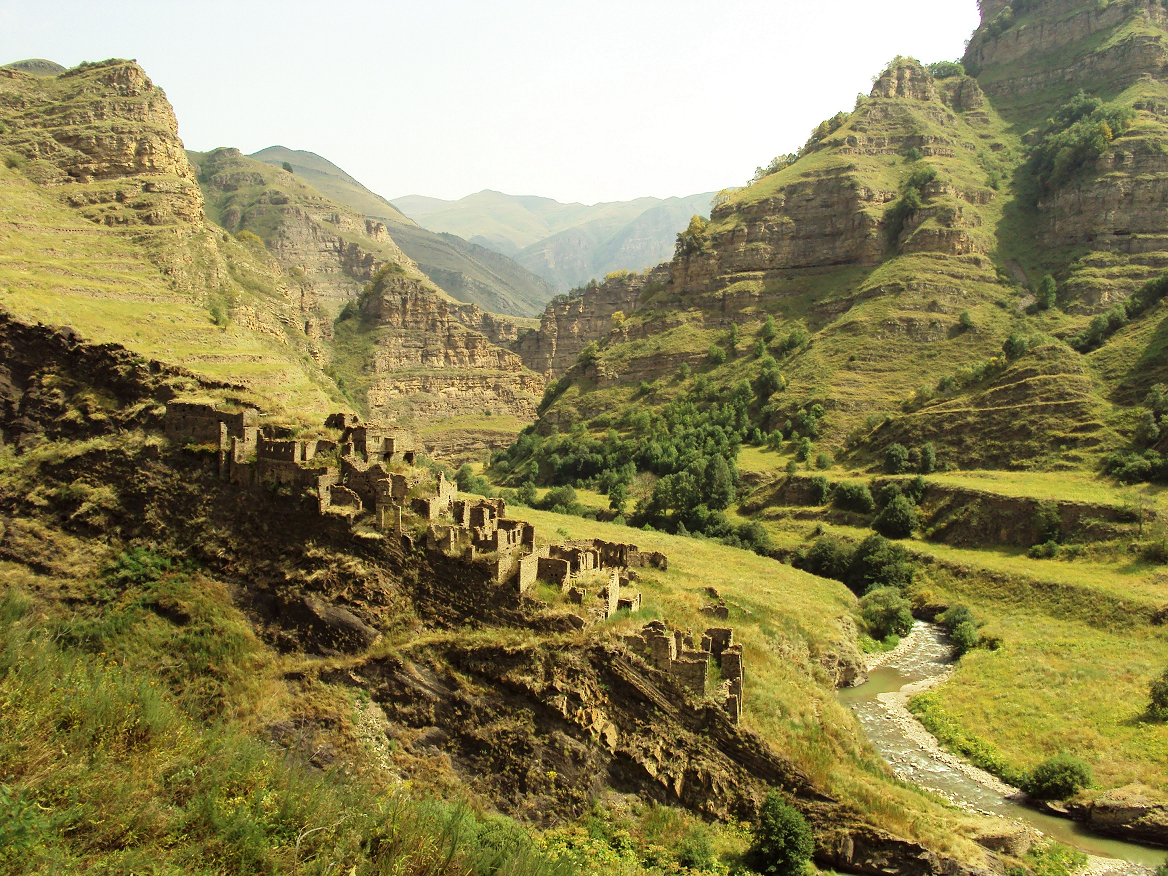
\includegraphics[scale=0.4]{figures/Sanzhi_1.png}
\end{figure}

\begin{figure}
	\caption{The village of Sanzhi in 2013 (courtesy of Iwona Kaliszewska)}
	\label{fig:Sanzhi 2}
	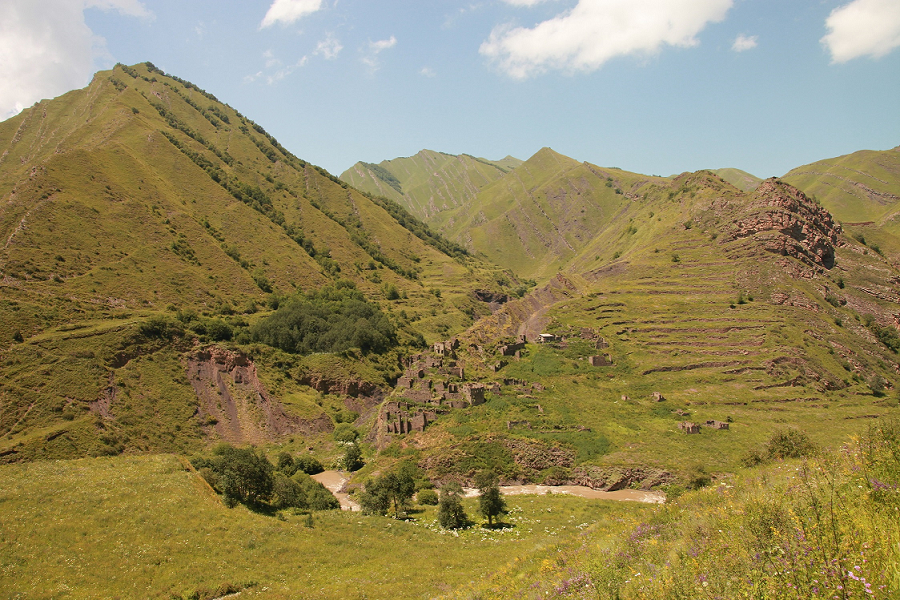
\includegraphics[scale=0.5]{figures/Sanzhi_2.png}
\end{figure}

\begin{figure}
	\caption{An old picture of Sanzhi, around 1957 (courtesy of the Sanzhi community)}
	\label{fig:Sanzhi 3}
	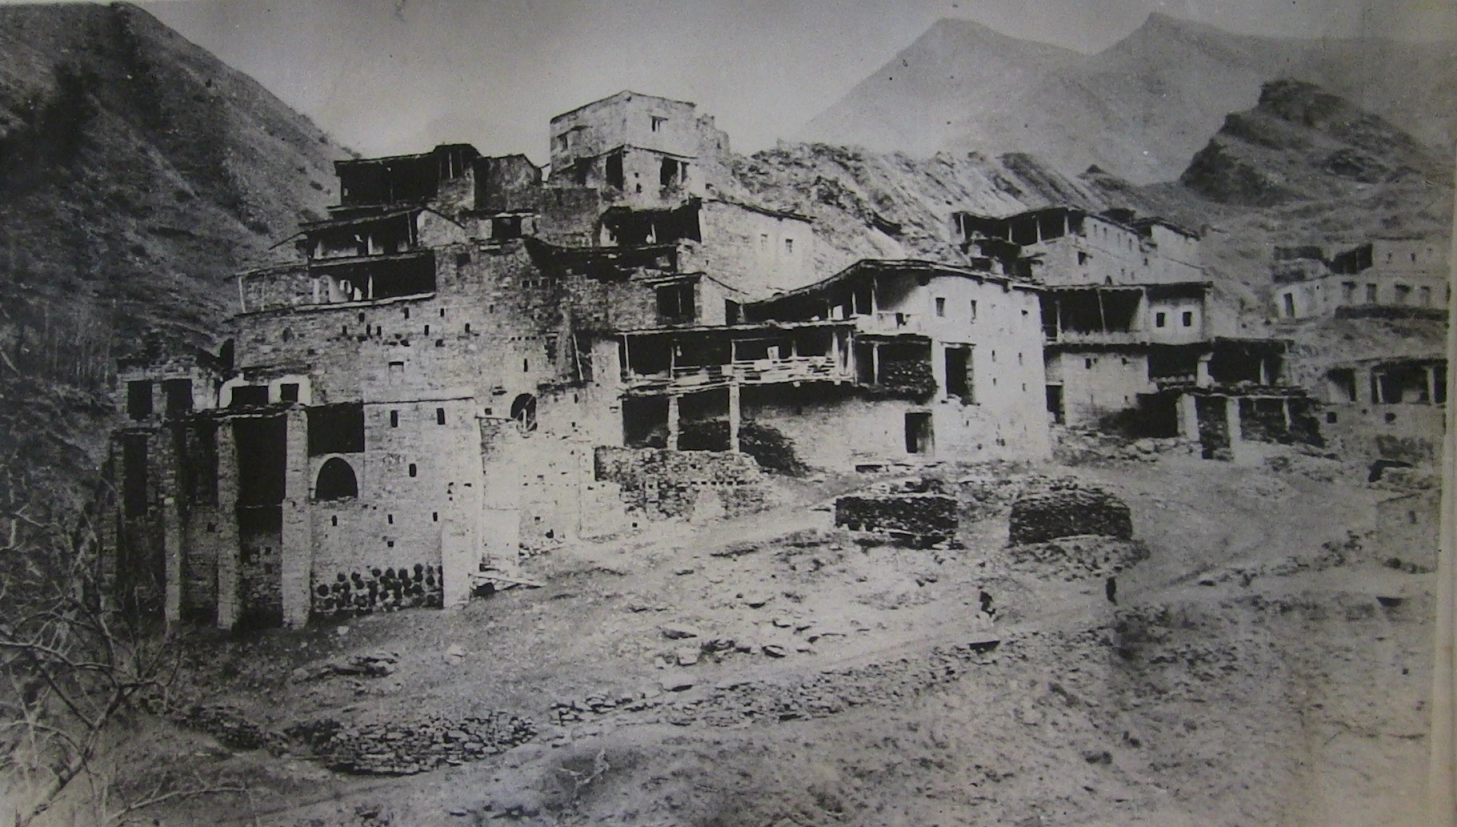
\includegraphics[scale=0.3]{figures/Sanzhi_3.png}
\end{figure}




From 1968 onwards, within a relatively short time span, all Sanzhi people moved to the lowlands to ethnically and linguistically mixed settlements. The major reason for the resettlement was the difficult life in the mountains. There was and still is no road leading to Sanzhi, and also no electricity. From grade five on, children had to walk by foot to the school in Itsari every day and in all weathers.

Today, the majority of Sanzhi speakers live in the village of Druzhba in the Dagestanian lowlands (Kayakentskiy Rayon) (\reffig{fig:Druzhba}) and to a lesser extent in other settlements in Dagestan and other parts of Russia. Druzhba is an ethnically and linguistically heterogeneous settlement with speakers of other South Dargwa varieties, other East Caucasian languages such as Tabasaran, Agul, Lezgian, and Lak, and also a very few Kumyk (Turkic) and Russian speakers. In Druzhba, people make a living by working in the local vineyards that used to be part of a \textit{sovkhoz} (Soviet state farm). Many inhabitants, especially men, commute to other parts of Russia to work there and support their families back home. A map of Dagestan with Sanzhi and Druzhba is given in \reffig{fig:Map 2}.

\begin{figure}
	\caption{The village of Druzhba in the winter of 2014 (picture by Diana Forker)}
	\label{fig:Druzhba}
	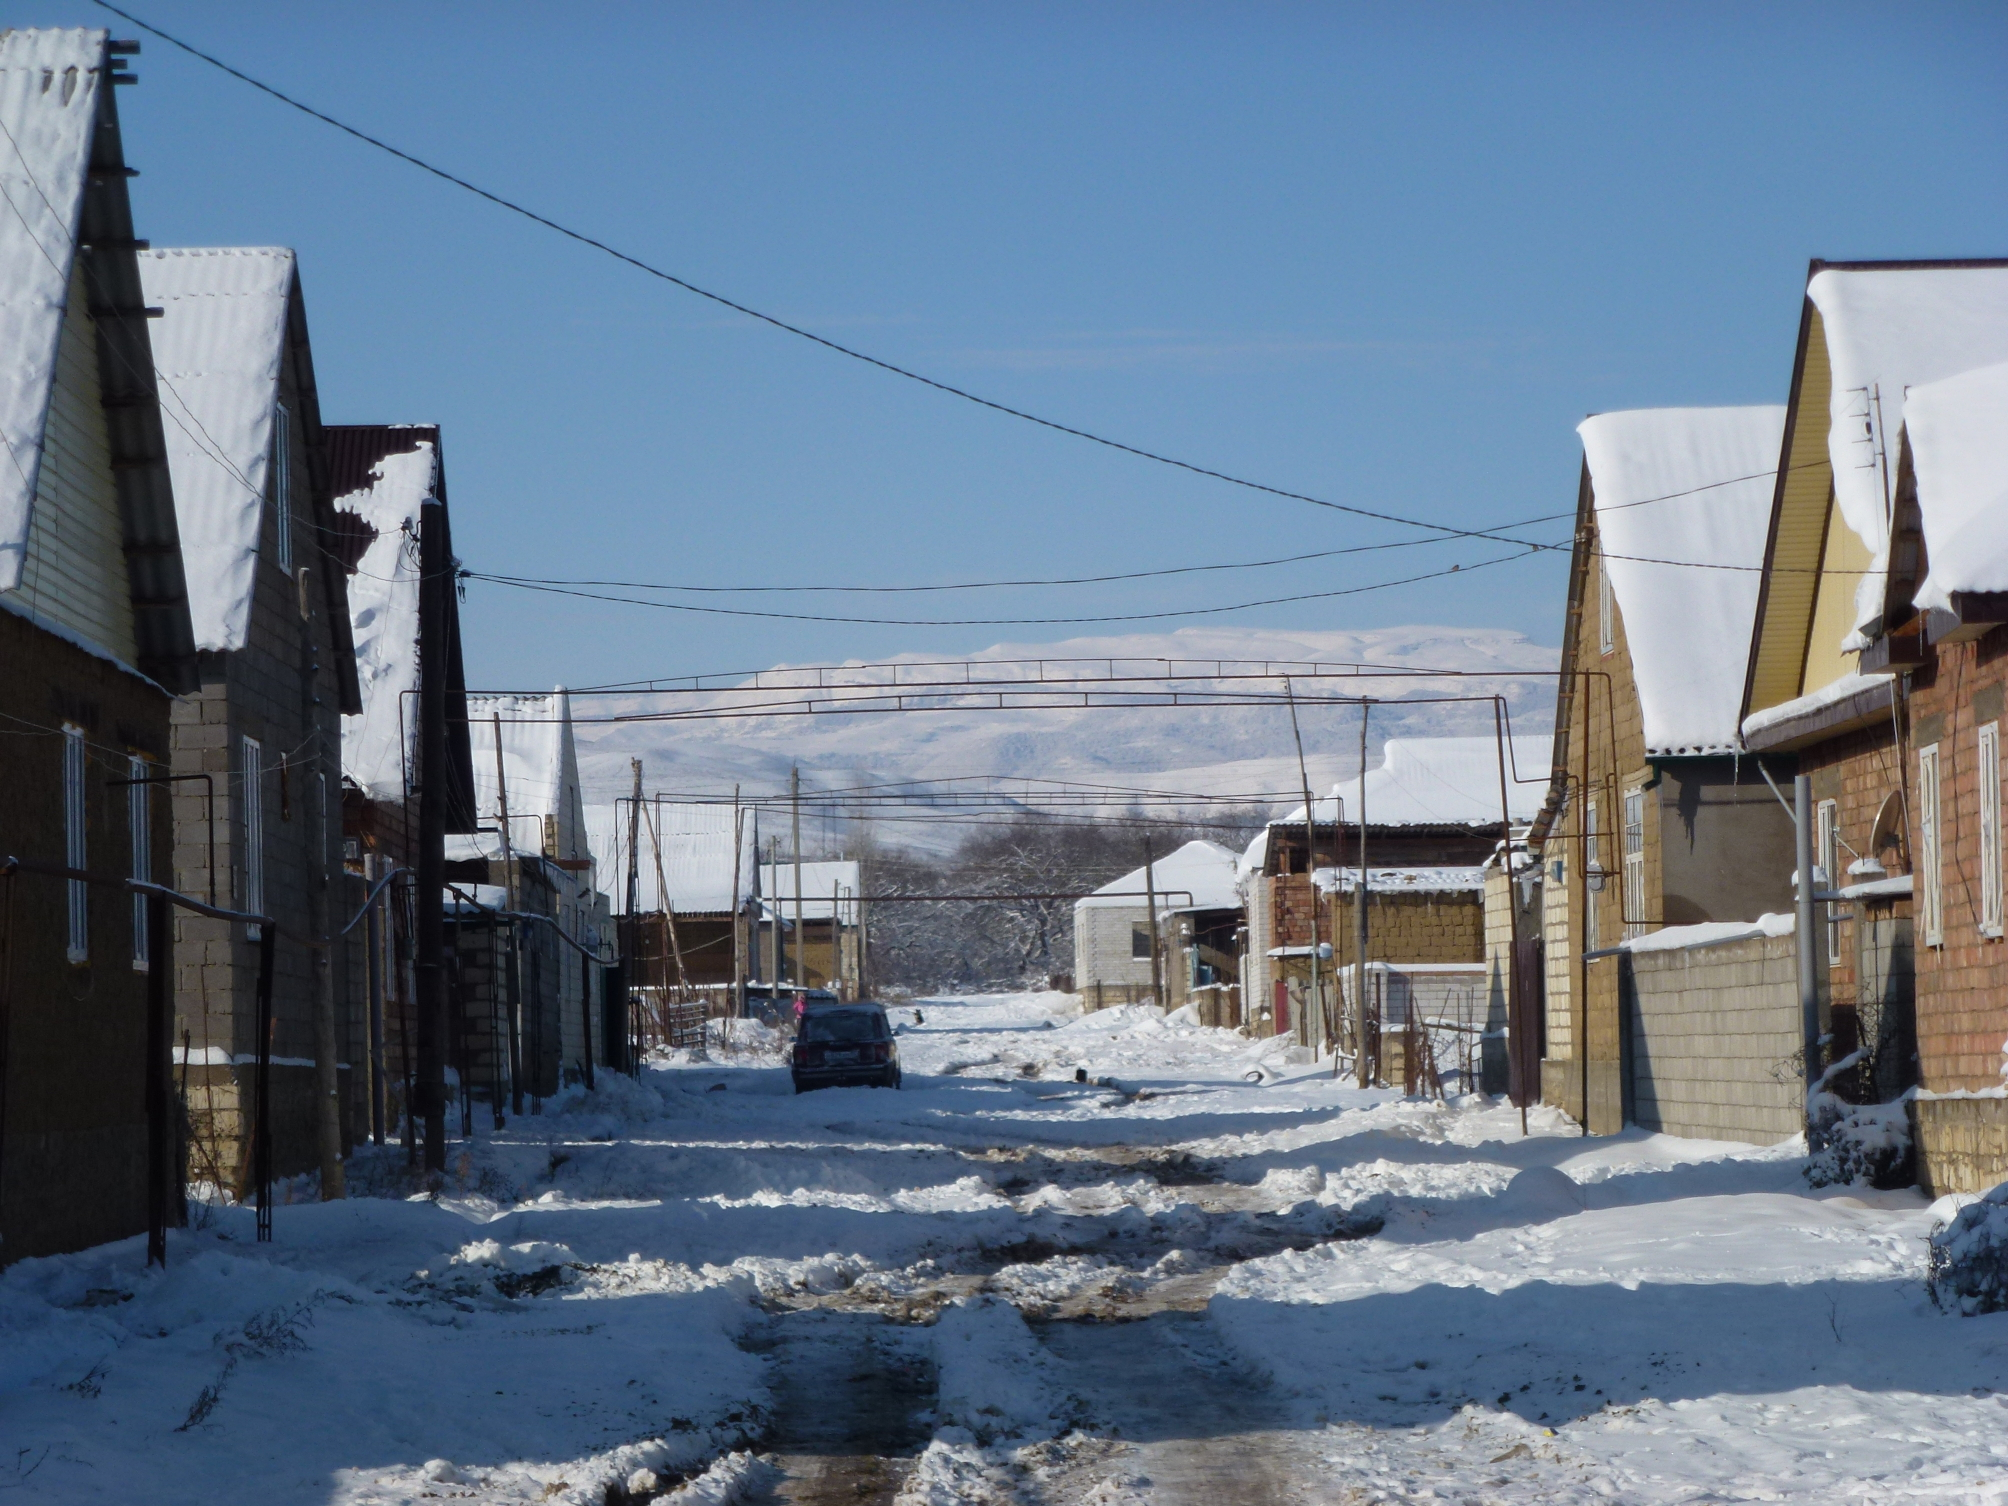
\includegraphics[scale=0.2]{figures/Druzhba.png}
\end{figure}


\begin{figure}[t!]
	\caption{Map of Dagestan}
	\label{fig:Map 2}
	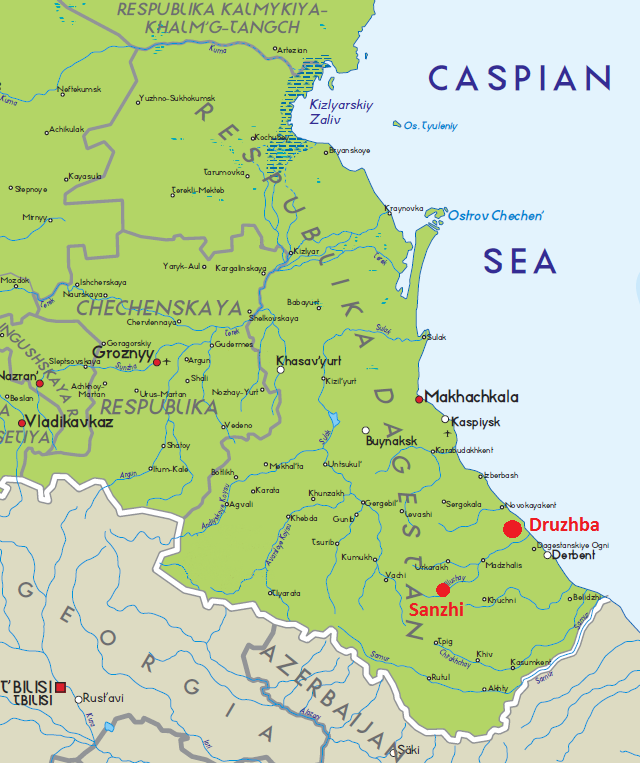
\includegraphics[scale=0.7]{figures/Dagestan_Sanzhi.png}
\end{figure}

%%%%%%%%%%%%%%%%%%%%%%%%%%%%%%%%%%%%%%%%%%%%%%%%%%%%%%%%%%%%%%%%%%%%%%%%%%%%%%%%

\section{The sociolinguistic situation of Sanzhi}
\label{sec:The sociolinguistic situation of Sanzhi}

All languages of the Republic of Dagestan are official languages, but only 14 of them have the status of being officially written languages. Sanzhi Dargwa, like many other comparatively small languages and varieties spoken on the territory of Dagestan, does not belong to the written languages.  

Before the arrival of Russian in the remote parts of the central Dagestanian mountains, where the original village of Sanzhi is located, Kumyk served as the language of interethnic communication in the wider area. The main traces of contact with Kumyk are the numerous Turkic loan words (e.g. the first part in \textit{ač barq'ij} `open' originates from the Kumyk verb \textit{ač-maq}, \textit{baχča} `garden' (identical in Kumyk), \textit{qːʷaz} `goose' from Kumyk \textit{qaz}, and many more). Nevertheless, among the Sanzhi speakers with whom I worked, nobody claimed to have a significant command of Kumyk. All villages, except for one\footnote{The exception is the village of Shara that was originally inhabitated by speakers of Agul, but today it is also a Dargwa village according to my Sanzhi assistant.} in the immediate neighborhood of Sanzhi, are Dargwa villages with Dargwa varieties closely related to Sanzhi, so that communication was and still is easily possible just by sticking to one's own variety.

\begin{figure}
	\caption{Sanzhi men at the Uraza Bayram, the holiday at the end of Ramadan in 2013 (Gadzhimurad Gadzhimuradov, who is dressed in dark clothes, is standing on the left side) (picture by Diana Forker)}
	\label{fig:SanzhiPeople}
	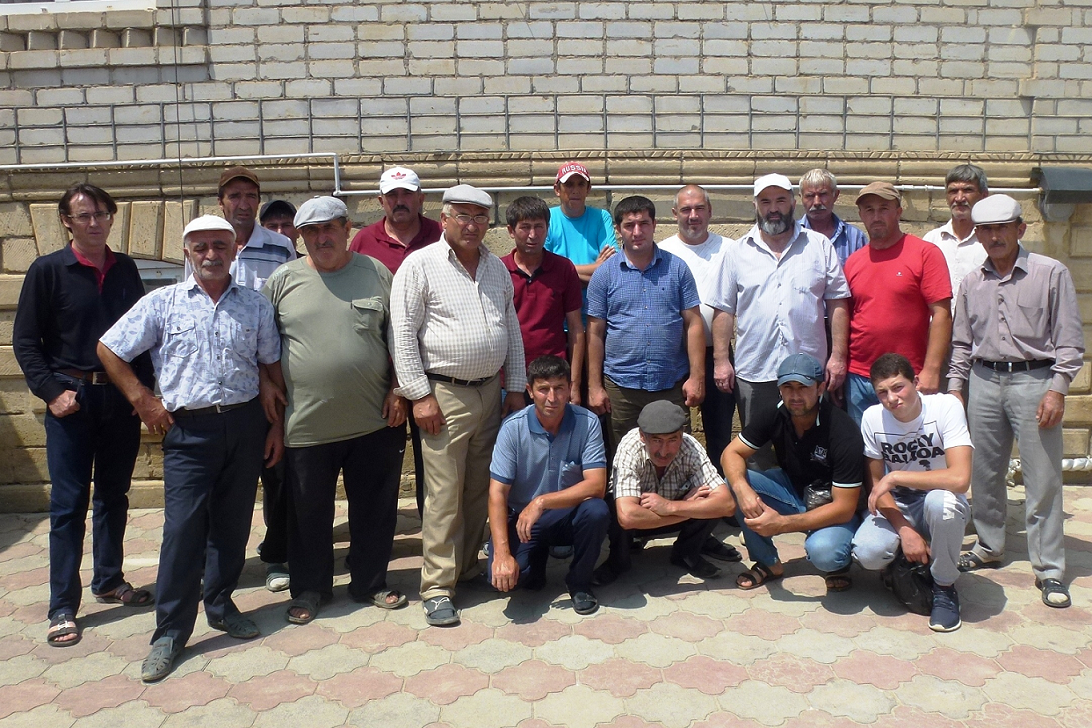
\includegraphics[scale=0.4]{figures/8_uraza2013.png}
\end{figure}

Today, all Sanzhi speakers are bilingual or multilingual to various extents because they know at least some Russian. Russian serves as the main language of interethnic communication and is the only language used in education and administration, and more generally in the public sphere in Dagestan. The degree of bilingualism varies from speaker to speaker, but simplifying somewhat, it is possible to say that women of the oldest generation (60 years and older) are the only group for whom Sanzhi is the dominant language. Men of the oldest generation as well as many members of the middle generation (age 30 to 60) are more or less balanced bilinguals, and use the two languages in accordance with the different functional domains (public/official vs. private/speech community). All members of the youngest generation are dominant in Russian, but everybody has at least a passive command of Sanzhi and is able to use a simplified form of the language in communication with members of the oldest generation, e.g. in interaction between grandchildren and grandparents.

Thus, the contact situation is largely language maintenance for the oldest and middle generation. Among the youngest generation language shift is observable, and it is reasonable to assume that members of the youngest generation in particular who are still children today will not pass on Sanzhi to their children. Some children and young people in Druzhba still learn Sanzhi as their first language (this depends on the family situation), but they come in contact with Russian right from the first day of their life. Russian becomes the dominant language at the latest when children start attending kindergarten. Therefore, they generally have a limited and mostly passive command of Sanzhi and prefer to speak only Russian. Sanzhi people of the young generation, including small children, speak predominantly Russian with each other. More and more Sanzhi people speak Russian not only to their neighbors in Druzhba, many of which are from other ethnic groups, but even at home. Although the people have a positive language attitude and are proud of speaking their own language, Russian is considered to be not only more prestigious, but extremely necessary for the future of their children (see \citealt{ForkerSubmitteda} for more information).

Another factor influencing the linguistic situation is marriage between women and men from different ethnic groups, which usually does not lead to bilingual children acquiring both the language of the mother and of the father, but to children speaking only Russian at home, as the parents use Russian to communicate with each other. I estimate that there are only a few families left in which both husband and wife are competent Sanzhi speakers that have grown up in the village of Sanzhi. We can assume that in the past the situation must have been different and the vast majority of wives were either from Sanzhi or from the surrounding villages (Itsari, Chakhri, Kunki, Duakar, Dzilebki are the main villages of origins of mothers and wives of the Sanzhi speakers with whom I worked).

Since Sanzhi Dargwa is not employed in the public domain (e.g. administration, education, media,  court) the language is unwritten and used only for oral communication within the Sanzhi community. The only printed material so far is \citet{Forker.Gadzhimuradov2017}, a collection of traditional stories and other texts. In school, Sanzhi children have around two hours of mother tongue education per week, during which they learn Standard Dargwa. Sanzhi speakers do not understand literary Standard Dargwa, because Akusha Dargwa, the base for the standard language, is a Northern Dargwa variety and quite different from Sanzhi. Therefore, in spite of the school classes, Sanzhi children usually do not learn Standard Dargwa well and are not able to speak, write, or read in Standard Dargwa, or make use of the few newspapers and TV programs that exist.



%%%%%%%%%%%%%%%%%%%%%%%%%%%%%%%%%%%%%%%%%%%%%%%%%%%%%%%%%%%%%%%%%%%%%%%%%%%%%%%%

\section{Genealogical affiliation}
\label{sec:Genealogical affiliation}

Sanzhi belongs to the Dargwa (Dargi) languages, which form a subgroup of the East Caucasian (Nakh-Dagestanian) language family. The exact \isi{number} of languages belonging to this family is unknown, but it can be estimated to be around 40. The internal classification of the family has not yet been unanimously resolved. \reffig{fig:classificationtree} shows one of the possible classifications (namely the classification according to \citealt[xi]{Kibrik1996}). The internal division of the Dargwa branch into subvarieties is largely taken from \citet{Korjakov2006}. Dargwa languages are commonly divided into a Northern Dargwa group and a Southern Dargwa group, whereby Sanzhi belongs to the latter. The spelling of the names for languages and varieties in  \reffig{fig:classificationtree} follows the conventions established in the literature and in the recent handbooks on East Caucasian languages \citep{PolinskyInPress, KoryakovEtAllInPreparation}. Unfortunately, in a few cases this leads to differences between the spelling of a village name and the spelling of the language spoken in it (e.g. the village of Itsari vs. Icari Dargwa).
%
\begin{figure}
	\caption{A family tree of East Caucasian}
	\label{fig:classificationtree}

	\small
	\begin{itemize}
		\item[]	Nakh branch
		\item[]	\qquad\tit{Chechen, Ingush, Tsova-Tush (Batsbi)}

		\item[]	Avar-Andic-Tsezic subbranch
		\item[]	\qquad Avar-Andic
		\item[] \qquad\qquad \textit{Avar}
		\item[]	\qquad\qquad Andic
		\item[]	\qquad\qquad\qquad\tit{Andi, Botlikh, Godoberi, Karata, Akhvakh, Bagvalal,} 
		\item[]	\qquad\qquad\qquad\tit{Tindi, Chamalal}

		\item[]	\qquad Tsezic subbranch
		\item[]	\qquad\qquad\tit{Tsez, Hinuq, Khwarshi, Bezhta, Hunzib}

		\item[]	Dargwa subbranch
		\item[]	\qquad\tit{Akusha/Standard Dargwa, Urakhi, Mugi, Tsudakhar, Gapshima-Butri,}
		\item[]	\qquad\tit{Mjurego-Gubden, Kadar, Muiri, Mehweb, Sirkhi, Amukh-Xuduc, Shiri,}
		\item[]	\qquad\tit{Qunqi, Icari, \tbf{Sanzhi}, Chirag, Kajtag, Kubachi-Ashti}

		\item[]	\tit{Lak}
		\item[]	\tit{Khinalug}

		\item[]	Lezgic subbranch
		\item[]	\qquad\tit{Udi, Archi, Lezgian, Agul, Tabasaran, Tsakhur, Rutul, Kryz, Budugh}
	\end{itemize}
\end{figure}


%%%%%%%%%%%%%%%%%%%%%%%%%%%%%%%%%%%%%%%%%%%%%%%%%%%%%%%%%%%%%%%%%%%%%%%%%%%%%%%%

\section{Dargwa languages and the problem of the \dqt{Dargwa ethnicity}}
\label{sec:Dargwa languages and the problem of the Dargwa ethnicity}

Today, all languages spoken in the the Republic of Dagestan have the status of official languages (see the article 11 of the constitution of Dagestan, 2003). This includes Standard Dargwa and Russian, among others. There is a distinction between the so-called ``unwritten'' and the ``written languages'' of Dagestan. The latter are (in addition to Russian), Avar, Agul, Azerbaijani, Kumyk, Lak, Lezgian, Noghay, Rutul, Tabasaran, Tat, Tsakhur, and Chechen. Written languages of Dagestan are, in principle, taught in school and used to some extent in the media (e.g. newspapers, journals). Until 1928, speakers of Dargwa varieties used the Arabic script, but there was no standard \isi{orthography}. From 1925 onwards, the first newspaper in a Dargwa language was published \citep[15]{Abdullaev1954}. This newspaper, as well as most books and other materials, was published in Akusha Dargwa, the language which was later chosen as the basis for the literary standard Dargwa language. There are several reasons for this choice: Akusha was and still is the Dargwa variety with the most speakers, and the village of Akusha together with the surrounding villages formed an autonomous center (\textit{vol'noe obščestvo}) for a long time. In 1930 at the first Dagestanian conference on \isi{orthography}, Akusha was appointed to be the basis for the literary standard Dargwa language. In 1928, a Latin alphabet was developed for a \isi{number} of Dagestanian languages including Dargwa, Avar, Lak, Lezgian, and Tabasaran. In 1938 the policy changed completely, and for all Dagestanian literary languages Cyrillic alphabets were introduced \citep[48\tnd51]{Grenoble2003}. In the following years the Dargwa alphabet underwent several changes.

Dargwa people are officially considered to be one group that shares a common ethnicity, and to speak various dialects of one and the same Dargwa language (see below for the viewpoint of linguistics on this). According to the data of the Russian census from 2010, for instance, about 510\ths000 people consider themselves to be ethnic Dargwa, and thus represent the second biggest ethnic group in Dagestan (after the Avars). The vast majority of them claim to speak Dargwa.

Dargwa languages are spoken in the central part of Dagestan (traditionally in the districts Akushinskiy, Levashinskiy, Dakhadayevskiy, Sergokalinskiy, Kaytagskiy, and also partially in the districts of Gunibskiy, Buynakskiy, Karabudakhkentskiy, and Agulskiy), in a territory with a length of about 100 km and a breadth of about 70 km (\reffig{fig:Map 3}). In the west, this area borders on Lak and Avar territory. In the north and east, the Dargwa area borders on Kumyk lands, and in the south on Tabasaran lands.


\begin{figure}[t!]
	\caption{The East Caucasian (i.e. Nakh-Dagestanian) language family (map courtesy of Yura Koryakov)}
	\label{fig:Map 3}
	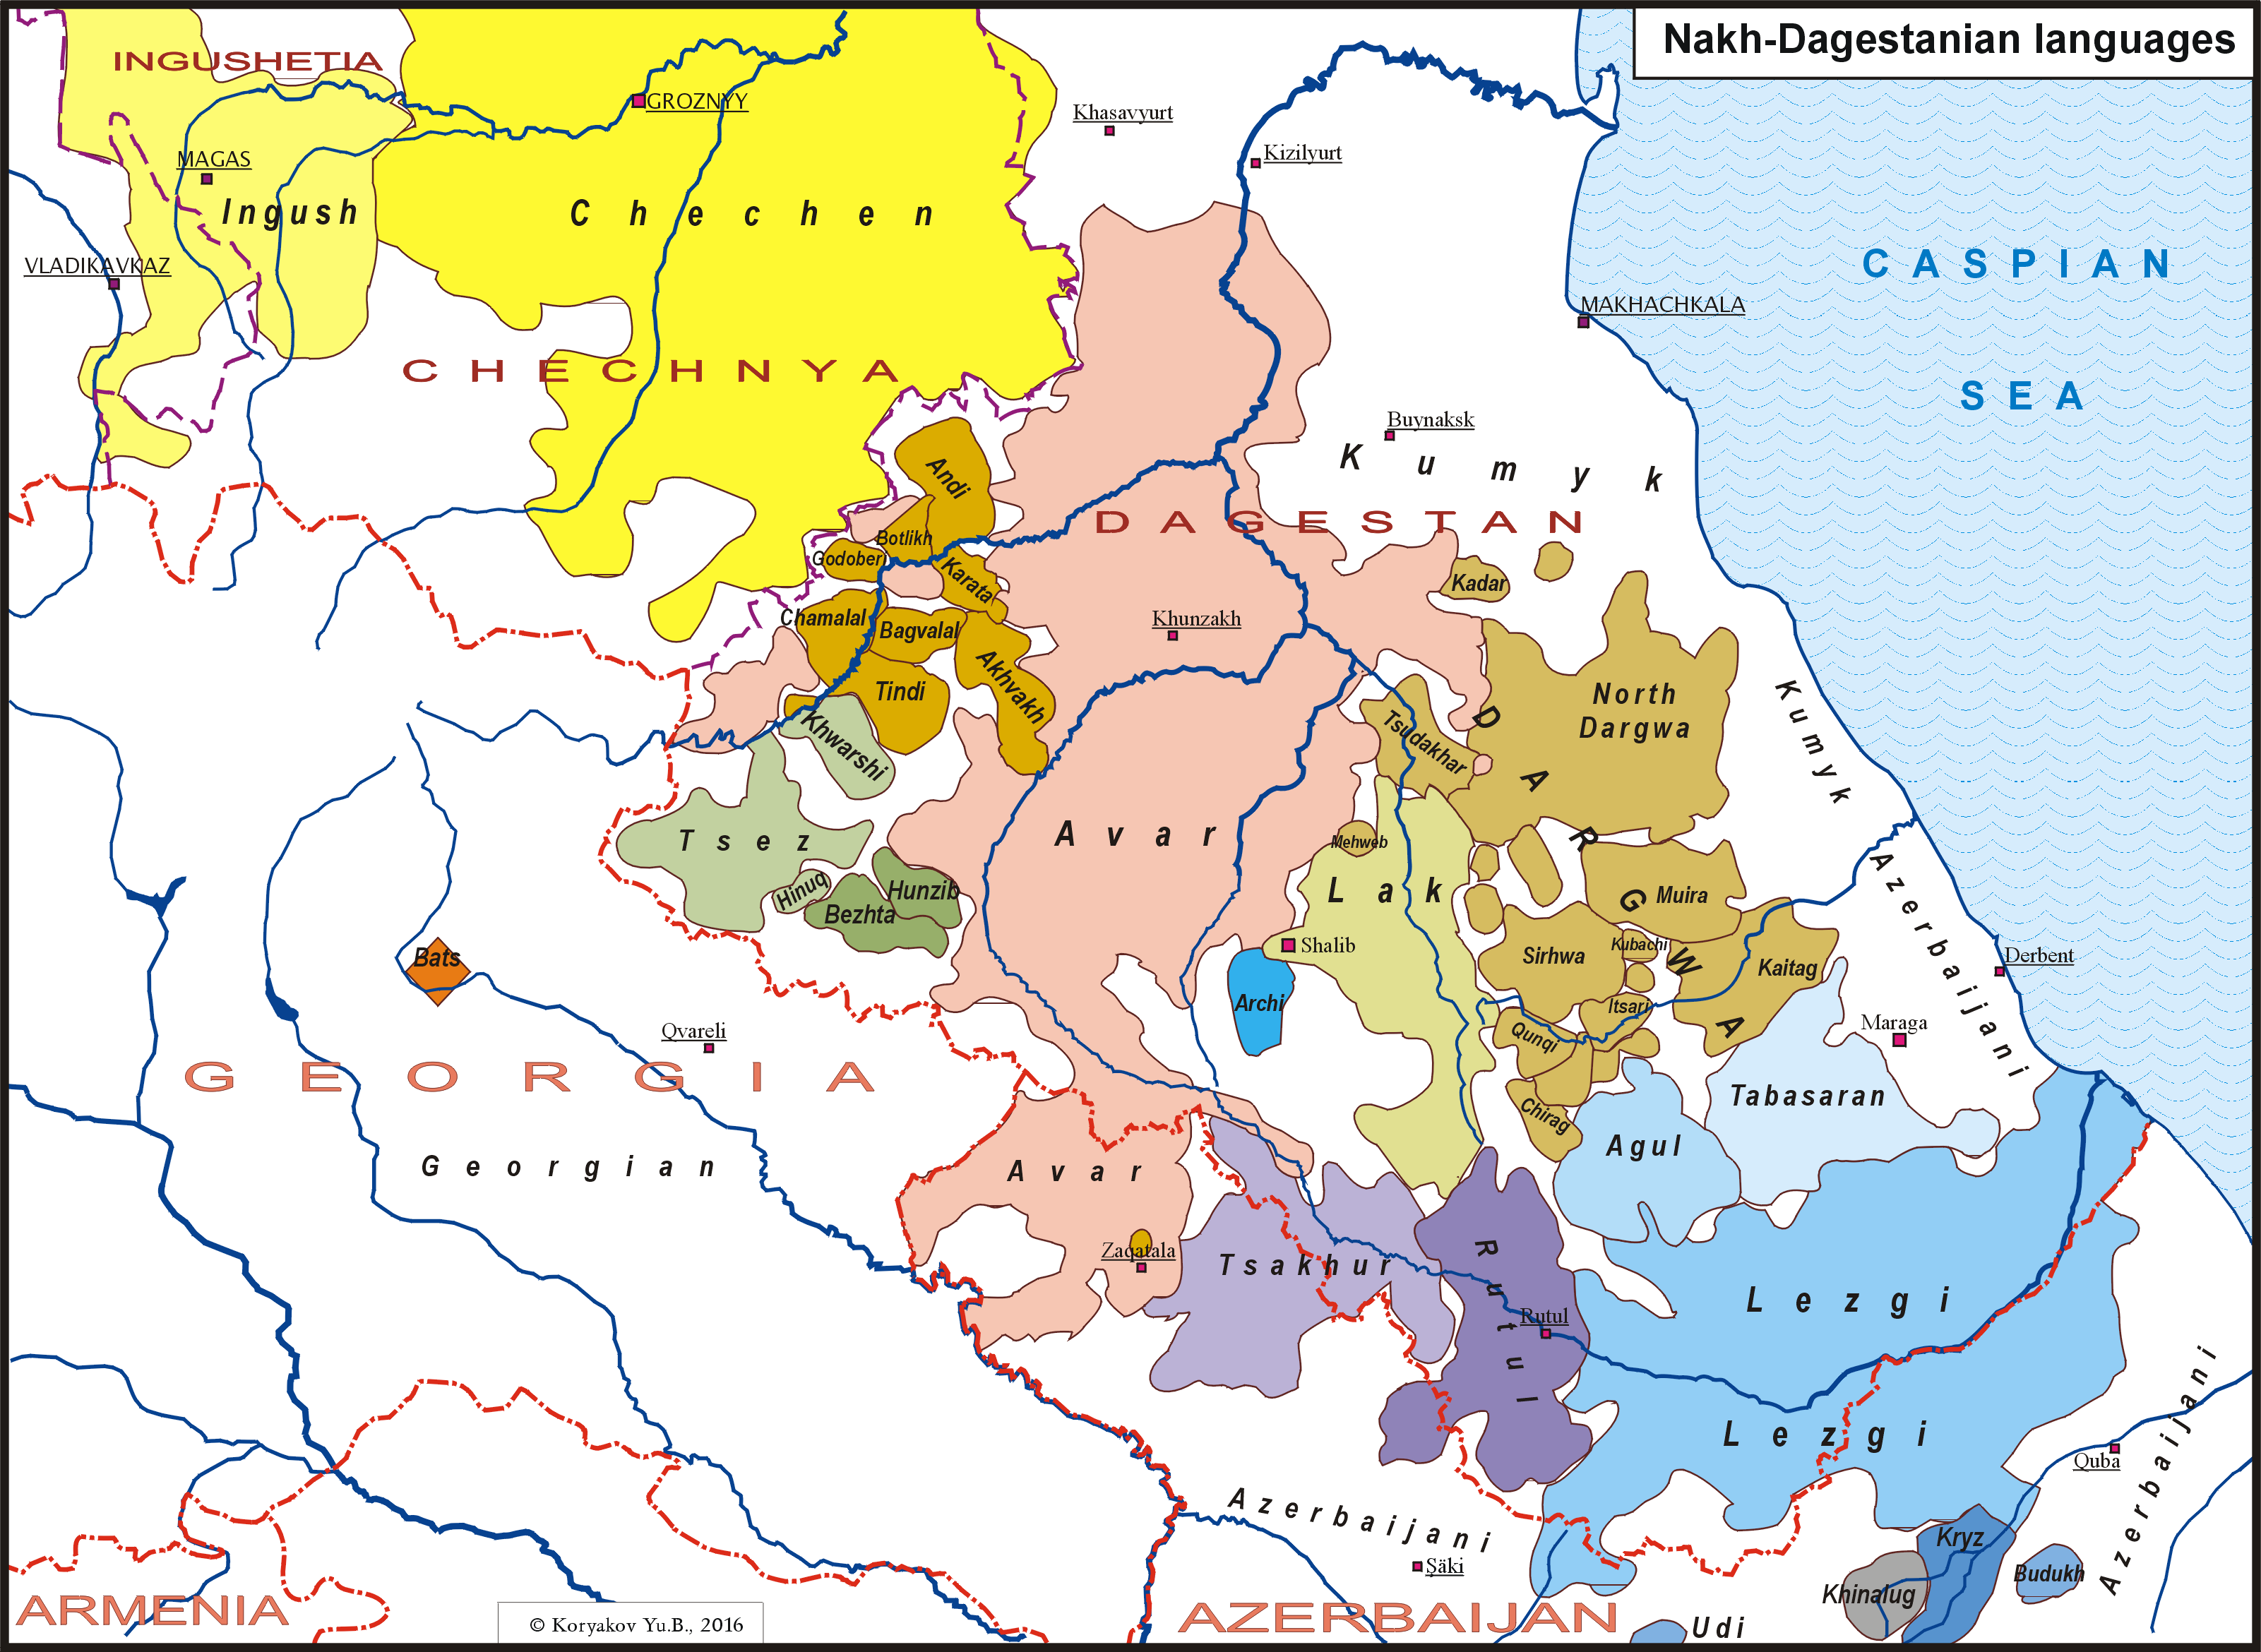
\includegraphics[scale=0.6, angle =90]{figures/NEC_color_2016.png}
\end{figure}

The term \textit{Dargwa} with its current reference was only introduced during Soviet times. There was a policy at the time to create names for peoples and languages that often lacked significance for the people themselves, and to introduce ethnic boundaries all over the Northern Caucasus \citep[114]{Grenoble2003}. The use of these names is nowadays fully established and is largely maintained for political reasons \citep{Shaxbanov2009}.

Historically, the term \textit{Dargwa} (or \textit{Dargi}) does not refer to an ethnic group \citep[13]{Abdullaev1954}. There were seven unions of settlements in central Dagestan that referred to themselves with a proper name and the term \textit{Dargwa}: Akusha Dargwa, Bukun Dargwa, Gutsi Dargwa, Kaba Dargwa, Utsmi (or Kaytag) Dargwa, Khamur Dargwa, and Sirkha Dargwa \citep[13]{Magomedov1999}. That is, \textit{Dargwa} referred to settlement centers that consisted of a \isi{number} of small villages forming a unit, which were able to defend themselves and their own interests against enemies (\textit{vol'noe obščestvo}). Other urban centers in the north, like Kadar and Gubden, whose inhabitants are also considered to be Dargwa people today (and to speak Dargwa varieties), did not belong to those units to which the term \textit{Dargwa} was applied. They formed one administrative unit with Kumyk villages \citep[12]{Abdullaev1954}, and used Kumyk as their lingua franca (\citealt{DobrushinaDanielKoryakov}; \citealt[58\tnd59]{Wixman1980}). 

Similarly, there was not one single language with the name \textit{Dargwa}, but a group of related languages, in reference to which the names of the urban centers were used \citep[1]{Uslar1892}. But since Soviet times, the classification of the Dargwa varieties as dialects of one and the same Dargwa language has persisted in many publications and in all official documents (e.g. \citeb{Abdullaev1954}; \citeb{Gasanova1971}; \citeb{Museav2002}; WALS\footnote{\url{http://wals.info/}}; Ethnologue\footnote{\url{http://www.ethnologue.com/}}).

Following the most recent publications on the internal classification of the East Caucasian language family \citep{Korjakov2006, Korjakov.Sumbatova2007}, the Dargwa branch consists of 19 languages and about 40 dialects (see \reffig{fig:classificationtree} above). The biggest are Akusha Dargwa (about 42\ths000 speakers), Urakhi Dargwa (ca.~35\ths 000), Mjurego-Gubden Dargwa (ca.~39\ths000), followed by Kajtag Dargwa (ca.~21\ths000), and Tsudakhar Dargwa (ca.~19\ths000). Speakers of many Dargwa languages do not understand speakers of other Dargwa varieties, and the variation between them is much bigger than between the Andic languages, another subbranch of the East Caucasian family. The break-up of the Proto-Dargwa language can be estimated to have occurred about two millennia ago (Sumbatova, p.c.). However, the exact \isi{number} of Dargwa languages is still subject to debate, because descriptions are lacking for many of the individual languages and dialects. Thus, \reffig{fig:classificationtree} will likely need to be corrected in the future.

The place of the Dargwa languages inside the East Caucasian family is also debated. Some authors consider them to form a separate branch of the East Caucasian language family \citep[142]{Gigineishvili1977, Kibrik1996}, others group them together with Lak \citep{Haspelmath1993, Korjakov2006, vandenBerg2005}.


%%%%%%%%%%%%%%%%%%%%%%%%%%%%%%%%%%%%%%%%%%%%%%%%%%%%%%%%%%%%%%%%%%%%%%%%%%%%%%%%

\section{Typological overview}
\label{sec:Typological overview}

Sanzhi Dargwa is typologically similar to other East Caucasian languages. It has a relatively large consonant inventory including pharyngeal and \isi{ejective} \isi{consonants}, and a medium \isi{number} of vowels. With respect to its morphosyntactic structure, Sanzhi is predominantly dependent-marking with a rich case inventory. The \isi{grammatical cases} are \isi{ergative}, \isi{absolutive}, \isi{dative}, and \isi{genitive}. In addition, there is a plethora of \isi{spatial cases}. The morphology is concatenative and predominantly suffixing. Sanzhi has an elaborate system of TAM forms. Verbal stems come in pairs that express imperfective and \isi{perfective aspect}, and many can take spatial \isi{preverbs}. Salient traits of the grammar are two largely independently operating agreement systems: \isi{gender}/\isi{number} agreement and \isi{person agreement}. Gender/\isi{number} agreement operates at the phrasal and at the clause level. Within the clause, it is mainly controlled by arguments in the \isi{absolutive} case and shows up on verbs, adverbs, and on \isi{nouns} in some of the \isi{spatial cases}. Person agreement operates at the clausal level only, and functions according to a person hierarchy. Sanzhi has \isi{ergative} alignment at the level of morphology. SOV is the most frequent \isi{constituent order}.

Features of Dargwa languages that have attracted the attention of typologists and linguists working within various theoretical frameworks include \isi{gender} and \isi{person agreement} \citep{Sumbatova2011, Sumbatova2013, Belyaev2013, Belyaev2017a, Belyaev2017b, GanenkovForthcoming, Forker2016a}, complement constructions including \isi{reported speech} \citep{Ganenkov2012, ForkerSubmittedb}, \isi{experiencer} constructions \citep{Comrie.vandenBerg2006, Ganenkov2006, Ganenkov2013}, local and \isi{long-distance reflexivization} \citep{Forker2014}, \isi{backward control} and long-distance agreement \citep{Serdobolskaya2009, Serdobolskaya2010, Belyaev2016}, the expression of space \citep{Ganenkov2010, ForkerLTSanzhi}, \isi{information structure} \citep{Sumbatova2009, Forker.Belyaev2016, Forker2016a}, and the problem of \isi{finiteness} \citep{Kalinina.Sumbatova2007}.


%%%%%%%%%%%%%%%%%%%%%%%%%%%%%%%%%%%%%%%%%%%%%%%%%%%%%%%%%%%%%%%%%%%%%%%%%%%%%%%%

\section[Literature and previous works]{Literature on Dargwa languages, Dargwa people, and previous works on Sanzhi}
\label{sec:Literature on Dargwa languages, Dargwa people, and previous works on Sanzhi}

In comparison to some other Dagestanian languages, the description of Dargwa languages has a relatively long tradition. However, despite the impressive \isi{number} of monographs and articles that have been dedicated to various Dargwa languages, the scope and the quality of many of these works cannot satisfy modern scientific standards. Thus, in the following I will mention only those works that are still in use and represent valuable documentations and analyses of Dargwa. For a more detailed overview on the history of the study of Dargwa languages, see \citet{Magometov1983} and also the references in \citet{Temirbulatova2005}.

The first scientific treatment of a Dargwa language (Urakhi) comes from \citet{Uslar1892}, who visited the Caucasus in the second half of the 19th century. The next key scholar is Said Abdullaev, who published a Russian-Dargwa (i.e. Akusha) dictionary and a grammar of Akusha \citep{Abdullaev1950, Abdullaev1954}. Since the 1950s, Saida Gasanova has written many articles and books about various Dargwa languages and dialects, concentrating mainly on Muiri, Mjuregi, Urakhi, and Tsudakhar \citep[e.g.][]{Gasanova1961, Gasanova1971}. Other important scholars are Zapir Abdullaev, who worked on Standard Dargwa and occasionally on Urakhi and Kajtag \citep[e.g.][]{Abdullaev1961, Abdullaev1969, Abdullaev1971, Abdullaev1986, Abdullaev1993, AbdullaevEtAl2014}, and Magomed-Said Musaev, who investigated various Dargwa varieties, including Chirag and Akusha \citep[e.g.][]{Musaev1975, Musaev1978, Musaev1983, Musaev1980a, Musaev1980b}. There are also works on Sikhi \citep{Kadibagomedov1998}, on Kajtag \citep{Temirbulatova2005} and most notably on Kubachi \citep{Magometov1963}. Recently, two new dictionaries have been published \citep{Jusupov2005, Jusupov2009}. Rasul Mutalov, one of the key participants in the language documentation project resulting in this grammar, has written a \isi{number} of papers and books on Icari Dargwa and Standard Dargwa \citep{Mutalov1992, Mutalov2002, Mutalov2018}.

In \citey{vandenBerg1999}, the first book in English on a Dargwa language (Akusha), written by \citea{vandenBerg1999} was published, followed by a descriptive grammar of Icari Dargwa, which was co-authored by Nina Sumbatova and Rasul Mutalov \citep{Sumbatova.Mutalov2003}. Icari Dargwa is closely related to Sanzhi Dargwa; the two varieties are mutually intelligible and the Icari grammar was a fruitful source of inspiration for this grammar of Sanzhi.

In Moscow, a group of linguists works on a \isi{number} of Dargwa languages, of which the major results are comprehensive studies of Tanti \citep{Sumbatova.Lander2014}, Shiri \citep{BelyaevInPreparation}, Mehweb \citep{DanielMehweb}, Ashti \citep{Belyaev2012} and Chirag \citep{GanenkovChiragSketch}. Other important works from the same group are \citet{Kalinina.Sumbatova2007}, \citet{Sumbatova2009, Sumbatova2010, Sumbatova2011, Sumbatova2013}, \citet{Lander2008, Lander2010}, and \citet{Serdobolskaya2009, Serdobolskaya2010}. \citet{SumbatovaInPreparation} provides a recent overview on Dargwa varieties. Sketch grammars in preparation include \citet{GanenkovChiragSketch} and \citet{ForkerSanzhiSketch}.

Topics in the morphosyntax of Sanzhi and other aspects of Sanzhi have been treated in \citet{Forker2016a, Forker2014, Forker2019, ForkerSubmitteda, ForkerSubmittedb, ForkerSubmittedc}. A collection of texts with Russian translations and a Sanzhi-Russian and Russian-Sanzhi dictionary is \citet{Forker.Gadzhimuradov2017}.

There is not much to say with respect to the ethnographic literature on Dargwa people. There are only two older monographs \citep{Schilling1949, Gadzieva.etal1967}.


%%%%%%%%%%%%%%%%%%%%%%%%%%%%%%%%%%%%%%%%%%%%%%%%%%%%%%%%%%%%%%%%%%%%%%%%%%%%%%%%

\section{Documenting and describing Sanzhi Dargwa}
\label{sec:Documenting and describing Sanzhi Dargwa}

This grammar is the result of a language documentation project, \tit{Documenting Dargi languages in Dagestan \tnd\ Shiri and Sanzhi}, funded by the DoBeS program of the Volkswagen Foundation. The project officially started in 2012 and ran until 2019. Within this project, three linguists (Diana Forker, Rasul Mutalov, Oleg Belyaev), one anthropologist (Iwona Kaliszewska), and student assistants from the Universities of Bamberg and Leipzig (André M{\"u}ller, Teresa Klemm, and Felix Anker) documented, described, and analyzed the two endangered East Caucasian languages Shiri Dargwa and Sanzhi Dargwa.

\sloppy Detailed information about the project, the languages and many texts, recordings and pictures can be found on the project website.\footnote{\url{http://www.kaukaz.net/dargwa/sanzhi/lexicon/index.htm}} All materials gathered in the project are accessible upon request via the Language Archive hosted by the MPI Nijmegen.\footnote{\url{http://dobes.mpi.nl/projects/shiri_sanzhi/}} The major results of the project are, in addition to the grammar of Sanzhi, a book with narratives, legends and other texts for the Sanzhi community \citep{Forker.Gadzhimuradov2017}, the electronic corpus of Sanzhi texts with audio recordings for every text and many video recordings (around 24 hours of natural speech), and an electronic dictionary. Around 15 hours of speech have been transcribed in ELAN, translated into Russian, and are deposited in the Language Archive.\footnote{\url{https://archive.mpi.nl/}} A subcorpus of around 10 hours, which amounts to more than 46\ths000 word tokens, has been fully glossed with FLEx\footnote{\url{https://software.sil.org/fieldworks/}} and translated into Russian and English. The texts have almost exclusively been recorded by myself in the village of Druzhba. During the recordings I was accompanied by Rasul Mutalov, my fellow project member, linguist and native speaker of the neighboring Icari dialect, or by Gadzhimuard Gadzhimuradov, my main language assistant, who led the conversation and explained the aims of the project to the Sanzhi speakers. After recording the text were transcribed in ELAN by using a Cyrillic \isi{orthography} (page xvii) and by making use of the help of native speakers. They also provided a Russian translation. In the ELAN file I added a Latin transliteration following the \isi{orthography}, which is also employed in this grammar (page xvii). From the transcribed texts I chose a subcorpus, transferred the Latin transcription into FLEx, glossed it and partially added English translations to the Russian translations.

The glossed corpus has been put on the internet and is freely is accessible.\footnote{\url{http://web-corpora.net/SanzhiDargwaCorpus/search/index.php?interface_language=en}} This corpus consists of 75 texts from 24 speakers of Sanzhi who were between 21 and 80 years old when the texts were recorded (mostly between 2012 and 2015). Only three of the speakers were 35 years or younger, whereas most were older than 50. Slightly more than half of the speakers were female, but the majority of texts originate from male speakers.

The corpus contains the following types of texts:

\begin{itemize}
	\item 32 fairy tales, legends, anecdotes
	\item 8 fairy tales translated from Standard Dargwa and Russian
	\item 10 autobiographical narrations and texts about the history of the village
	\item 4 recipes and other instructions or procedural texts
	\item 3 poems
	\item 3 natural conversations
	\item 11 descriptions, conversations and narratives from the \textit{\textit{Family Problems Picture Task}} \citep{SanRoqueEtAl2012} (additionally archived with PARDISEC, in the collection SocCog\footnote{\url{http://catalog.paradisec.org.au/collections/SocCog}})
	\item 4 narrations produced by means of stimuli (two ``Pear Stories'', two stories ``Frog, where are you?'') 
\end{itemize}

The natural data has been complemented by many hours of elicitation. All natural examples originating from the corpus are not further marked in this grammar. All examples which have been elicited are marked by (E).

% https://corpus1.mpi.nl/ds/asv/;jsessionid=2E07D70EB3228292714D678A5572555D?0&openpath=node:1615060



\sloppy The electronic dictionary of Sanzhi was built up with Lexique Pro\footnote{\url{http://www.lexiquepro.com/}} and has been published with \textit{Dictionaria}.\footnote{\url{https://dictionaria.clld.org/contributions/sanzhi}} The dictionary contains around than 5\ths500 entries written with Cyrillic and Latin script, Russian and English translations, grammatical information, and example sentences as well as audio recordings for (almost) every entry. The dictionary is also accessible via the project homepage\footnote{\url{http://www.kaukaz.net/dargwa/sanzhi/lexicon/index.htm}}.

In August 2017, my main assistant Gadzhimurad Gadzhimuradov and I were able to print a book with community materials and present it to the Sanzhi community in Druzhba (\reffig{fig:SanzhiBook}). The book contains 42 texts of various genres taken from the corpus (fairy tales, legends, anecdotes, descriptions of games and recipes, oral history, and a poem) written in the Cyrillic Sanzhi script with a sentence-by-sentence translation in Russian, as well as a Sanzhi-Russian and a simplified Russian-Sanzhi dictionary, which is also available on the project website.

Within the project I have undertaken more than ten field trips to Druzhba (including two short trips to Sanzhi in 2013 and 2016) in order to gather materials on the language. My major language assistant and consultant during all these years was and is Gadzhimurad Gadzhimuradov (\reffig{fig:SanzhiPeople}), a videographer and cameraman from Druzhba, who was born in Sanzhi. After spending his first five years there, his family moved to Druzhba, but he has ever since kept close relationships with the village and is a strong patriot in the best sense. Without the support and friendship of him and his family, in particular his wife Batichay, neither the grammar nor the entire project could have been realized. Gadzhimurad Gadzhimuradov not only helped me to gather, transcribe, and translate materials, he also made many recordings by himself, translated texts into Sanzhi and raised the interest of the Sanzhi community in the project. Patiently he sat down endless hours with me to go through morphological and syntactic paradigms. This grammar could not have been written without his assistance.



\begin{figure}
	\caption{Gadzhimurad Gadzhimuradov presenting the first book in Sanzhi (courtesy of Gadzhimurad Gadzhimuradov, 2017)}
	\label{fig:SanzhiBook}
	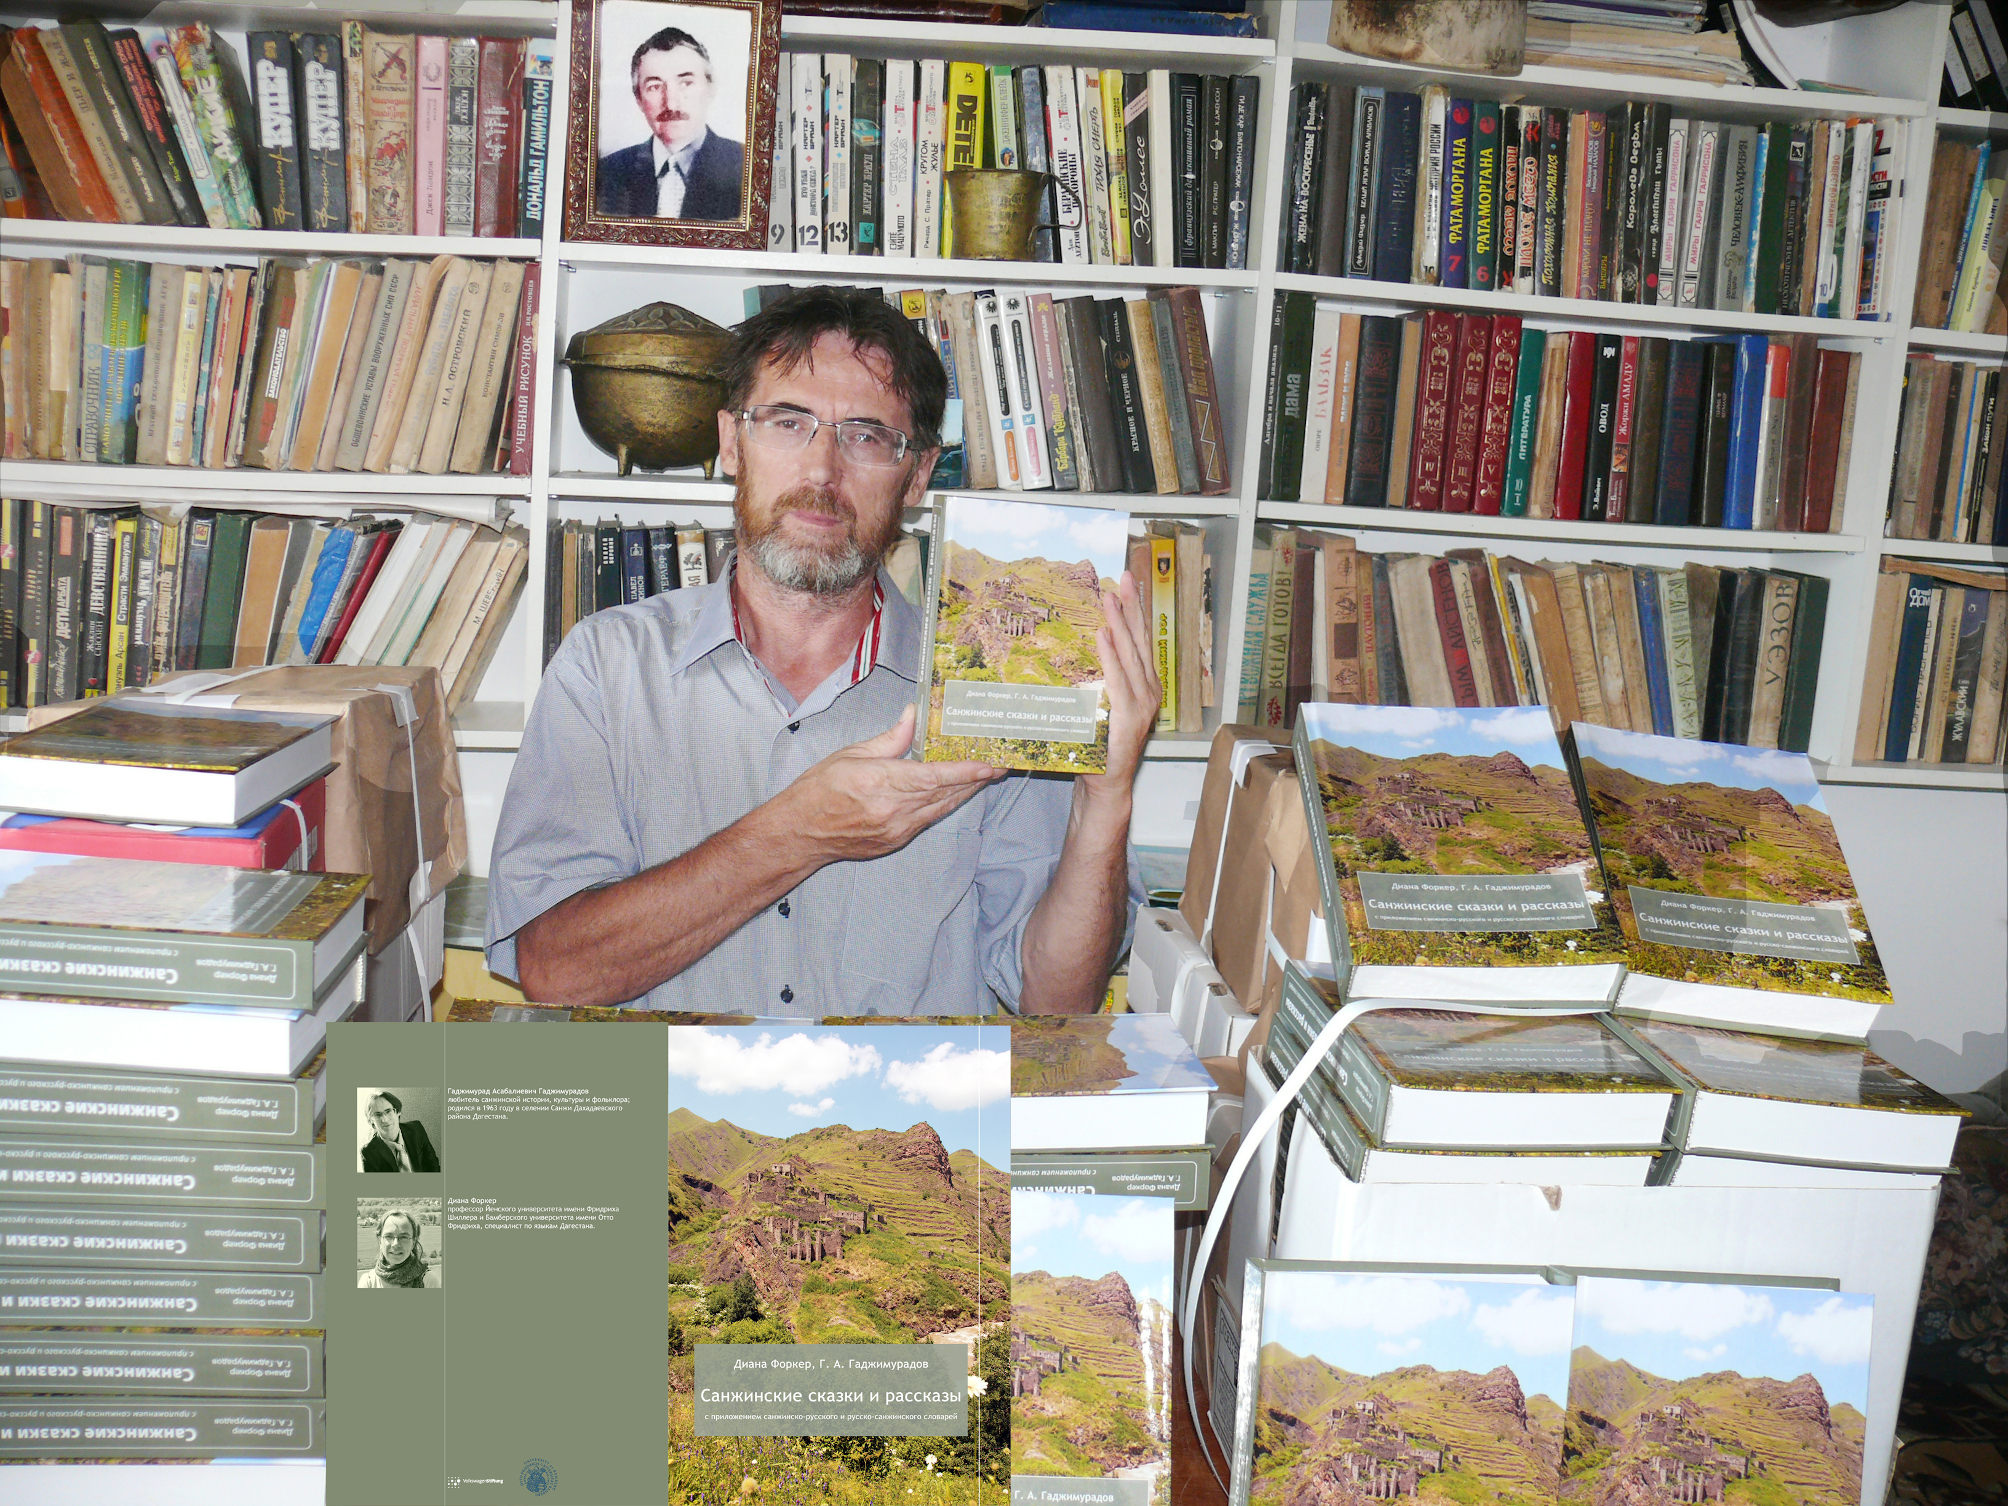
\includegraphics[scale=0.1]{figures/SanzhiBooks1.png}
\end{figure}


\chapter{Phonology}
\label{cpt:phonology}

Sanzhi phonology is typical for East Caucasian languages with its relative large consonant inventory (\refsec{sec:Consonant inventory}) and medium vowel inventory (\refsec{sec:Vowel inventory}). Other topics covered in this chapter are the \isi{syllable structure} (\refsec{sec:Syllable and word structure}), \isi{pharyngealization} (\refsec{sec:Pharyngealization}), \isi{stress} (\refsec{sec:Word stress}), and phonological and morphophonological alternations (\refsec{sec:Phonological and morphophonological alternations}). 


%%%%%%%%%%%%%%%%%%%%%%%%%%%%%%%%%%%%%%%%%%%%%%%%%%%%%%%%%%%%%%%%%%%%%%%%%%%%%%%%

\section{Consonant inventory}
\label{sec:Consonant inventory}

\reftab{tab:The consonant inventory of Sanzhi Dargwa} displays the consonant inventory for Sanzhi. The table gives the phonemic value of the \isi{consonants} and  displays the orthographic representation used in this grammar in italics (see also page xvii for the Cyrillic \isi{orthography}). The three series of stops are, in the order given in the table: voiceless non-\isi{ejective}, voiced, and voiceless \isi{ejective}. The two series of fricatives are voiceless and voiced. All velars and uvulars also occur in labialized form. All voiceless non-\isi{ejective} stops and fricatives (except for the pharyngeal/epiglottal and the glottal sounds) also occur as geminates (i.e. tense).
%
\begin{table}\footnotesize
	\caption{The consonant inventory of Sanzhi Dargwa\label{tab:The consonant inventory of Sanzhi Dargwa}}
	\begin{tabularx}{1\textwidth}{Q c@{ }c@{ }c     c@{ }c@{ }c  c@{ }c c c@{ }c@{ }c c@{ }c c c}
		\lsptoprule
		& 	\multicolumn{3}{c}{\rotatebox{90}{bilabial}}
		& 	\multicolumn{3}{c}{\rotatebox{90}{alveolar}}
		& 	\multicolumn{2}{c}{\rotatebox{90}{postalv}}
		& 	\rotatebox{90}{palatal}
		& 	\multicolumn{3}{c}{\rotatebox{90}{velar}}
		& 	\multicolumn{2}{c}{\rotatebox{90}{uvular}}
		& 	\rotatebox{90}{pharyngeal/epiglottal}
		&	\rotatebox{90}{glottal}\\\midrule
			stop		& /p/ 	& /b/ 	& /pʼ/ 	& /t/ 	& /d/ 	& /tʼ/	& {} 	& {} 	& {} 	& /k/ 	& /ɡ/ 	& /kʼ/ 	& /q/ 	& /qʼ/ 	& /ʡ/ 	& /ʔ/\\
			{}		& \tit{p} & \tit{b} & \tit{pʼ} & \tit{t} & \tit{d} & \tit{tʼ} & {} & {} & {} & \tit{k} & \tit{g} & \tit{kʼ} & \tit{q} & \tit{qʼ} & \tit{ʡ} & \tit{ʔ}\\
			{}		& {}	& {} 	& {} 	& {} 	& {} 	& {}	& {} 	& {} 	& {} 	& /kʷ/ 	& /ɡʷ/ & /kʼʷ/	& /qʷ/ & /qʼʷ/	& {} 	& {}\\
			{}		& {} 	& {} 	& {} 	& {} 	& {} 	& {} 	& {} 	& {} 	& {} 	& \tit{kʷ} & \tit{gʷ}	& \tit{kʼʷ} & \tit{qʷ} & \tit{qʼʷ} & {} & {}\\
			{}		& /pː/ 	& {} 	& {} 	& /tː/	& {} 	& {} 	& {} 	& {} 	& {} 	& /kː/ 	& {} 	& {} 	& /qː/ 	& {} 	& {} 	& {}\\
			{}		& \tit{pː } 	& {} & {} & \tit{tː }	& {} & {} & {} 	& {} 	& {} 	& \tit{kː } & {} & {} 	& \tit{qː } & {} & {} 	& {}\\
			{}		& {}	& {}	& {}	& {}	& {}	& {}	& {}	& {}	& {}	& /kːʷ/	& {}	& {}	& /qːʷ/	& {}	& {}	& {}\\
			{}		& {}	& {}	& {}	& {}	& {}	& {}	& {}	& {}	& {}	& \tit{kːʷ} & {} & {}	& \tit{qːʷ} & {}	& {}	& {}\\\midrule

			fricative	& {}	& {}	& {}	& /s/ 	& /z/	& {}	& /ʃ/	& /ʒ/	& {}	& {}	& /x/	& {}	& /χ/	& /ʁ/	& /ħ/	& /h/\\
			{}		& {}	& {}	& {}	& \tit{s}	& \tit{z}	& {}	& \tit{š}	&  \tit{ž}	& {}	& {}	& \tit{x}	& {}	& \tit{χ}	& \tit{ʁ}	& \tit{ħ}	& \tit{h}\\
			{}		& {}	& {}	& {}	& {}	& {}	& {}	& {}	& {}	& {}	& {}	& /xʷ/	& {}	& /χʷ/ & /ʁʷ/	& {}	& {}\\
			{}		& {}	& {}	& {}	& {}	& {}	& {}	& {}	& {}	& {}	& {}	& \tit{xʷ}	& {}	& \tit{χʷ} 	& \tit{ʁʷ}	& {}	& {}\\
			{}		& {}	& {}	& {}	& /sː/	& {}	& {}	& /ʃː/	& /ʃː/	& {}	& {}	& /xː/	& {}	& /χː/	& {}	& {}	& {}\\
			{}		& {}	& {}	& {}	& \tit{sː}& {}	& {}	& \tit{šː}	& \tit{šː} & {}	& {}	& \tit{xː} & {}	& \tit{χː} & {}	& {}	& {}\\
			{}		& {}	& {}	& {}	& {}	& {}	& {}	& {}	& {}	& {}	& {}	& {}	& {}	& /χːʷ/	& {}	& {}	& {}\\
			{}		& {}	& {}	& {}	& {}	& {}	& {}	& {}	& {}	& {}	& {}	& {}	& {}	& \tit{χːʷ} & {} & {}	& {}\\\midrule

			affricate	& {}	& {}	& {}	& /t͡s/ & /t͡sʼ/	& {}	& /t͡ʃ/	& /t͡ʃʼ/ & {}	& {}	& {}	& {}	& {}	& {}	& {}	& {}\\
			{}		& {}	& {}	& {}	& \tit{c} & \tit{cʼ} & {} & \tit{č} & \tit{čʼ}  & {} & {} & {} & {}	& {}	& {}	& {}	& {}\\
			{}		& {}	& {}	& {}	& /t͡sː/	& {}	& {}	& /t͡ʃː/	& {}	& {}	& {}	& {}	& {}	& {}	& {}	& {}	& {}\\
			{}		& {}	& {}	& {}	& \tit{cː} & {} & {}	& \tit{čː}	& {} & {} & {}	& {}	& {}	& {}	& {}	& {}	& {}\\\midrule

			nasal		& {}	& /m/	& {}	& {}	& /n/	& {}	& {}	& {}	& {}	& {}	& {}	& {}	& {}	& {}	& {}	& {}\\
			{}		& {}	& \tit{m} & {} & {}	& \tit{n} & {} & {}	& {}	& {}	& {}	& {}	& {}	& {}	& {}	& {}	& {}\\\midrule

			liquid		& {}	& {}	& {}	& /r/	& /l/	& {}	& {}	& {}	& {}	& {}	& {}	& {}	& {}	& {}	& {}	& {}\\
			{}		& {}	& {}	& {}	&  \tit{r}	& \tit{l} & {} & {} & {} & {}	& {}	& {}	& {}	& {}	& {}	& {}	& {}\\\midrule

			semivowel		& {}	& /w/	& {}	& {}	& {}	& {}	& {}	& {}	& /j/	& {}	& {}	& {}	& {}	& {}	& {}	& {}\\
					& {}	& \tit{w} & {} & {}	& {}	& {}	& {}	& {}	& \tit{j} & {} & {}	& {}	& {}	& {}	& {}	& {}\\
		\lspbottomrule
	\end{tabularx}
\end{table}

The uvular stops /q/ and /qʷ/ have strong friction that makes them sound almost like affricates /q͡χ/ and /q͡χʷ/. The friction is absent from the \isi{ejective} /q'/ and the geminates /qː/ and /qːʷ/.

The phonemic glottal stop is found in the noun \tit{beʔe} \sqt{blood} and at the end of some words, for instance in the root-final position of two verbs \tit{ha-ʔ-} (\tsc{pfv})\slash\tit{h-erʔ-} (\tsc{ipfv}) \sqt{say} and \tit{b-erʔ-} (\tsc{pfv})\slash\tit{b-uʔ-} (\tsc{ipfv}) \sqt{rot} and the numeral \tit{kːaʔ-al} \sqt{eight}. Except for \tit{beʔe} \sqt{blood}, only loan words and names contain the glottal stop in root-medial position (e.g. \tit{daʔim} \sqt{continuation}, in the male name \tit{žaˁbraˁʔil}).

A non-phonemic glottal stop, which is not written, occurs before word-initial non-pharyngealized vowels, e.g. \tit{aba} [ʔaba] \sqt{mother}, including vowel-initial words in compounds, for example \tit{ca-ibil} [t͡saʔibıl] \sqt{first} (one\tsc{-ord}), or occasionally at other morpheme boundaries of inflected words, for example, \tit{a-uk-un}  \sqt{not eating} (\tsc{neg-}eat\tsc{.ipfv-icvb}) can be pronounced [aʔukʊn] or [aʊ̯kʊn].

The semivowel /w/ is realized as a voiced labiodental fricative [v] or as a labial-velar approximant [w]. 

In addition to the segments listed in \reftab{tab:The consonant inventory of Sanzhi Dargwa}, the voiceless labiodental fricative /f/ is attested in the \isi{ideophone} \tit{uf b-ik'ʷ-ij} \sqt{blow} (whew \tsc{hpl-}say\tsc{.ipfv-inf}) and in loan words, mostly from Russian, e.g. \textit{forel} \sqt{trout}. In older loans it had been replaced with /p/, e.g. \textit{purma} \sqt{uniform} (< \textit{forma}).

All plain \isi{consonants} occur in word-initial, word-medial, and word-final position. Geminates are never found in syllable-final position. Three labialized \isi{consonants} (/q'ʷ/, /χʷ/, /ʁʷ/) are also not attested in syllable-final position. \reftab{tab:Distribution of consonants@A} shows the \isi{distribution of consonants} by means of example words. The table contains a \isi{number} of morphologically complex words for which the relevant sound happens to occur at the end of the root, but within the stem because the root is followed by suffixes (the root is given in boldface). 
%
\begin{table}
	\caption{Distribution of consonants}
	\label{tab:Distribution of consonants@A}
	\footnotesize
	\begin{tabularx}{1\textwidth}[]{%
		>{\raggedright\arraybackslash\itshape}p{10pt}
		>{\raggedright\arraybackslash\hangindent=0.5em\itshape}X
		>{\raggedright\arraybackslash\hangindent=0.5em\itshape}X
		>{\raggedright\arraybackslash\hangindent=0.5em\itshape}X}

		\lsptoprule
 			{}	&	\upshape initial			&	\upshape medial			&	\upshape final\\
		\midrule
			p	&	puq'a \sqtx{nest}			&	qupi \sqtx{hoe}			&	t'up \sqtx{finger}\\
			b	&	bec' \sqtx{wolf}			&	heba \sqtx{then}			&	urχːab \sqtx{mill}\\
			p’	&	p'aq' \sqtx{shake off}		&	q'aˁp'i \sqtx{shutter}		&	lap' \sqtx{wave}\\
			pː	&	pːiħaˁla \sqtx{feather}		&	k'apːur \sqtx{leaf}			&	\tmd\\
			t	&	tum \sqtx{hill}			&	kːaˁta \sqtx{cat}			&	it \sqtx{that}\\
			d	&	du \sqtx{1\tsc{sg}}			&	juldaš \sqtx{friend}			&	ca-d \sqtx{is} \upshape(\tsc{cop}-\tsc{n})\\
			t’	&	t'up \sqtx{finger}			&	kːat'i \sqtx{scarf}			&	t'ult' \sqtx{bread}\\
			tː	&	tːaˁm \sqtx{trap}			&	tːutːu \sqtx{beak}			&	\tmd\\	   
			k	&	kabc \sqtx{skin, fell}		&	dukala \sqtx{apron}		&	dek \sqtx{dung}\\
			g	&	gurmedi \sqtx{type of kerchief}	&	zigar \sqtx{hurry}			&	dig \sqtx{meat}\\
			k’	&	k'apːur \sqtx{leaf}			&	nik'a \sqtx{little, small}		&	hek' \sqtx{this/that (up)}\\
			kʷ	&	kʷač'a \sqtx{paw}			&	mikʷa \sqtx{fingernail}		&	nekʷ \sqtx{straw}\\
			gʷ	&	gʷargʷal \sqtx{onion}		&	targʷa \sqtx{weasel}		&	mergʷ \sqtx{lair, den}\\
			kʼʷ	&	k'ʷel \sqtx{two}			&	r-\textbf{ik'ʷ}-ij\footnote{The relevant roots of morphologically complex words are given in boldface. In these words, the respective sound occurs at the end of the root, but within the stem because the root is followed by suffixes.} \sqtx{say} \upshape(\tsc{f-}say\tsc{.ipfv-inf})	&	erk'ʷ \sqtx{river}\\
			kː	&	kːaˁta \sqtx{cat}			&	kːalkːi \sqtx{tree}			&	\tmd\\
			kːʷ	&	kːʷacːa \sqtx{mare}			&	\textbf{akːʷ}-ar \sqtx{without} \upshape(\tsc{cop.neg-prs}) &	\tmd\\
			q	&	qaˁr \sqtx{pear}			&	b-aqil \sqtx{much}			&	qːaq \sqtx{back}\\
			q’	&	q'aˁp'i \sqtx{shutter}		&	puq'a \sqtx{nest}			&	aq' \sqtx{flock}\\
			qʷ	&	qʷesːa \sqtx{ashes}			&	ha-\textbf{lqʷ}-an  \sqtx{the climbing one} \upshape(\tsc{up}-direct\tsc{.ipfv-ptcp}) & daˁrqʷ \sqtx{barn}\\
			qʼʷ	&	q'ʷaˁl \sqtx{cow}			&	b-\textbf{elq'ʷ}-ij \sqtx{break} \upshape(\tsc{n-}break\tsc{.pfv-inf})		&	\tmd\\
			qː	&	qːap \sqtx{sack}			&	qːuˁlqːuˁ \sqtx{scythe}		&	\tmd\\
			qːʷ	&	qːʷaz \sqtx{goose}			&	\textbf{miriqːʷ}-e  \sqtx{worms} \upshape(worm\tsc{-pl})		&	\tmd\\
			s	&	sala \sqtx{in front, before}	&	qusmuk \sqtx{cupboard}		&	dus \sqtx{year}\\
			z	&	zija \sqtx{horsefly}			&	zize \sqtx{strawberry}		&	keruz \sqtx{slope}\\
			sː	&	sːika \sqtx{bear}			&	musːa \sqtx{place}			&	\tmd\\
			š	&	šal \sqtx{direction, side}		&	haniša \sqtx{summer}		&	juldaš \sqtx{friend}\\
			ž	&	žergʷa \sqtx{wasp}			&	ižal \sqtx{today}			&	hež \sqtx{this}\\
			šː	&	šːi \sqtx{village}			&	dešːa \sqtx{ancient}		&	\tmd\\
			x	&	xujal \sqtx{five}			&	xurxe \sqtx{sobber}		&	c'erx \sqtx{fat}\\
			xʷ	&	xʷit' \sqtx{whistle} (\isit{ideophone})	&	\textbf{ixʷ}-le \sqtx{early}			&	dirixʷ \sqtx{fog}\\
			xː	&	xːamxːa \sqtx{foam}			&	dirxːa \sqtx{stick}			&	\tmd\\
			χ	&	χat'a \sqtx{bowl}			&	alχni \sqtx{saw}			&	maχ \sqtx{barrow}\\
			ʁ	&	ʁajal \sqtx{twenty}			&	pːurʁum \sqtx{carriage}		&	qːabaʁ \sqtx{pumpkin}\\
			χʷ	&	χʷal-le \sqtx{much, a lot}		&	b-\textbf{iχʷ}-ij  \sqtx{be, become} \upshape(\tsc{n-}be\tsc{.pfv-inf})	&	\tmd\\
			ʁʷ	&	ʁʷab \sqtx{ploughshare}		&	aʁʷal \sqtx{four}			&	\tmd\\
			χː	&	χːula \sqtx{big, tall}			&	duχːu \sqtx{clever}			&	\tmd\\
	\end{tabularx}
\end{table}
\begin{table}
	%\caption{Distribution of consonants (cont.)}
	%\label{tab:Distribution of consonants@B}
	\footnotesize
	\begin{tabularx}{1\textwidth}[]{%
		>{\raggedright\arraybackslash\itshape}p{10pt}
		>{\raggedright\arraybackslash\hangindent=0.5em\itshape}X
		>{\raggedright\arraybackslash\hangindent=0.5em\itshape}X
		>{\raggedright\arraybackslash\hangindent=0.5em\itshape}X}

		\midrule
 			{}	&	\upshape initial			&	\upshape medial			&	\upshape final\\
		\midrule
			χːʷ	&	χːʷe \sqtx{dog}			&	ha-d-\textbf{erχːʷ}-ij \sqtx{fulfill} \upshape(\tsc{up}\tsc{-n-}fulfill\tsc{.pfv-inf}) &	\tmd\\
			c	&	ca \sqtx{one}			&	q'aca \sqtx{he-goat}		&	kabc \sqtx{skin, fell}\\
			c’	&	c'il \sqtx{then}			&	imc'a \sqtx{superflous}		&	bec' \sqtx{wolf}\\
			cː	&	cːab \sqtx{sky}			&	kːancːa \sqtx{step}			&	\tmd\\
			č	&	čina-b \sqtx{where\tsc{-n}}	&	ʡaˁči \sqtx{work}			&	deč \sqtx{drinking}\\
			čʼ	&	č'an \sqtx{wind, storm}		&	kʷač'a \sqtx{paw}			&	ʡaˁmč' \sqtx{May it peel off!} \upshape(peel\tsc{.pfv.opt})\\
			čː	&	čːaˁʡaˁl \sqtx{tomorrow, morning} &	ečːa \sqtx{she-goat}		&	\tmd\\
			ʔ	&	aba \sqtx{mother}			&	beʔe \sqtx{blood}			&	b-aʔ \sqtx{begin}\\
			ħ	&	ħaˁšak \sqtx{pot}			&	pːiħaˁla \sqtx{feather}		&	ʡaˁħ \sqtx{good}\\
			ʡ	&	ʡaˁbal \sqtx{three}			&	čːaˁʡaˁl \sqtx{tomorrow, morning}&	daˁʡ \sqtx{face}\\
			h	&	hel \sqtx{that}			&	buhem \sqtx{bundle}		&	b-ah \sqtx{owner}\\
			m	&	mikʷa \sqtx{fingernail}		&	gurmendi \sqtx{type of kerchief}	&	t'em \sqtx{smell}\\
			n	&	nekʷ \sqtx{straw}			&	haniša \sqtx{summer}		&	arin \sqtx{too much}\\
			r	&	rucːi \sqtx{sister}			&	rursːi \sqtx{girl, daughter}		&	q'ar \sqtx{herbs}\\
			l	&	lazun \sqtx{dough}			&	ʡuˁla \sqtx{wheel}			&	hel \sqtx{that}\\
			w	&	weral \sqtx{seven}			&	gawhar \sqtx{pupil}		&	alaw \sqtx{around}\\
			j	&	jangi \sqtx{new}			&	zija \sqtx{horsefly}			&	hej \sqtx{this}\\
		\lspbottomrule
	\end{tabularx}
\end{table}

Final voiced stops do not undergo devoicing. Final voiceless non-\isi{ejective} stops (/p/, /t/, /k/, /q/) are post-aspirated. Stops in final position are released. They are also released when a homorganic consonant follows, e.g. \tit{urek-c'al} \sqt{sixty}, \tit{ħaˁžat-ce} \sqt{necessary} (need\tsc{-dd.sg}), \tit{c'elt-ne} \sqt{gravestone\tsc{-pl}}, \tit{le-d=nu} (exist-\tsc{npl=prt}). If the voiceless stops /t/, /k/, or the voiceless affricate /t͡s/ occur at morpheme boundaries and are followed by homorganic \isi{consonants}, all \isi{consonants} are fully pronounced and released \refex{ex:gemination A phon}. Neither /t/ nor /k/ nor /t͡s/ become geminates under the described conditions, although gemination is otherwise a frequent process that applies across morpheme boundaries (\refsec{ssec:Gemination and degemination}). However, the \isi{ejective} stop /k’/ can turn into a plain stop as shown in the examples in \refex{ex:ikka phon}.
%
\begin{exe}
	\ex	\label{ex:gemination A phon}
	\begin{xlist}
		\ex	\tit{b-uˁc-ce}\slash\tit{b-uˁc-te} \sqt{thick} (\tsc{n-}thick\tsc{-dd.sg}\slash\tsc{n-}thick\tsc{-dd.pl})	\label{ex:bucce phon}
		\ex	\tit{tunt-ce}\slash\tit{tunt-te} \sqt{daring}	\label{ex:tuntce phon}
		\ex	\tit{ik'-ka} / \tit{hek'-ka} \sqt{from that} (\tsc{dem.up}\tsc{-abl}) (alternatively \tit{ik-ka} / \tit{hek-ka})
		\label{ex:ikka phon}
	\end{xlist}
\end{exe}

All velar and uvular \isi{consonants} occur in plain and labialized forms. The labialized velars and uvulars can be followed by all vowels except /u/. Labialization is mostly found with syllable-initial \isi{consonants}, but as \reftab{tab:Distribution of consonants@A} shows, there are also words with labialized \isi{consonants} in final position. In most words, \isi{labialization} is restricted to one consonant per root, but there are a \isi{number} of words with two labialized \isi{consonants}, e.g. \tit{gʷagʷa} \sqt{flower}, \tit{gʷargʷal} \sqt{onion}, and \tit{xʷixʷit'} \sqt{pipe}. In addition to \isi{labialization} in roots, deletion of the vowel /u/ triggers \isi{labialization} of the preceding consonant or following consonant (\refsec{ssec:Labialization and delabialization}). Labialized \isi{consonants} are mostly found in \isi{nouns}, numerals, \isi{adjectives}, adverbs, and verbs and also attested in a few \is{particle}particles, but not in pronouns or suffixes. Labialization is absent from Standard Dargwa and therefore speakers who have been trained in the Standard Dargwa \isi{orthography} do not write them in Sanzhi, although they pronounce them. Younger speakers often replace labialized \isi{consonants} by plain \isi{consonants} and change a preceding or following \tit{a} to \tit{o} (in speech and writing). Minimal pairs for some labialized \isi{consonants} are given in \refex{ex:labialization phon@A}.
%
\begin{exe}
	\ex	\label{ex:labialization phon@A}
	\begin{xlist}
		\TabPositions{14em}
		\ex	\tit{d-elq'-ij} (\tsc{pfv}) \sqt{grind}	\tab \tit{d-elq'ʷ-ij} (\tsc{pfv}) \sqt{break}\label{ex:delqij phon}
		
		\ex	\tit{b-iχ-ij} (\tsc{pfv}) \sqt{tie, fasten}	\tab \tit{b-iχʷ-ij} (\tsc{pfv}) \sqt{be, become, be able}	\label{ex:bixwij phon}
		\ex	\tit{akri} \sqt{Akri} (place name)	\tab \tit{akʷri} \sqt{be not} (\tsc{cop.neg.msd}) \label{ex:akri phon}
		\ex	\tit{ik'-i-j} \sqt{for this / that up}	\tab \tit{ik'ʷ-ij} \sqt{say}	(say\tsc{.m.ipfv-inf}) \label{ex:ikwij phon}\\
		(\tsc{dem.up}\tsc{-obl-dat}) 
	\end{xlist}
\end{exe}

Geminates are always voiceless, non-\isi{ejective}, and unaspirated. All voiceless non-\isi{ejective} obstruents, except for pharyngeal/epiglottal and glottal segments, occur as geminates, and even a \isi{number} of labialized \isi{consonants} are geminates. The phonemic status of geminates is proven by the minimal pairs and minimal oppositions in \refex{ex:gemination B phon@A}.
%
\begin{exe}
	\ex	\label{ex:gemination B phon@A}
	\begin{xlist}
\TabPositions{14em}
		\ex	\tit{iχ-i-j} \sqt{for this / that down}	\tab \tit{iχː-ij} \sqt{guard, protect, care}	\\
		(\tsc{dem.down}\tsc{-obl-dat})
		\ex	\tit{b-uq-ij} (\tsc{pfv}) \sqt{run, go} \tab \tit{b-uqː-ij} \sqt{carry, bring}	\label{ex:buqij phon}
	
		\ex	\tit{bus-ij} \sqt{rain}	\tab \tit{b-usː-ij} \sqt{sleep, fall asleep} \label{ex:busij phon}
		
		\ex	\tit{b-ač-ij} (\tsc{pfv}) \sqt{smear, spread} \tab \tit{ačː-ij} \sqt{strike, hit onself} 	\label{ex:bacij phonA}
		
		\ex	\tit{b-ac-ij} (\tsc{pfv}) \sqt{plough} \tab \tit{acːi-j} \sqt{to the uncle} (uncle\tsc{-dat})	\label{ex:bacij phonB}
		\ex	\tit{het-i-j} \sqt{for that} (\tsc{dem-obl-dat}) \tab \tit{hetːi} \sqt{those}	\label{ex:hetij phonC}
		
	\end{xlist}
\end{exe}

Geminate fricatives are not always easy to identify because fricatives can be tense in emphatic pronunciation. But geminate stops and affricates are clearly audible as such, because there is a significant difference in the closure duration between singletons and geminates. Gemination can probably be analyzed as a difference between lax and tense \isi{consonants}, but the exact phonetic properties of geminates still need to be clarified by future research.

In addition to their occurrence in stems, geminates occur at morpheme boundaries (see \refsec{ssec:Gemination and degemination} below). A few sonorants can also occur as tense \isi{consonants} within roots (/n/, /m/, /l/, /r/, and /w/) and/or at morpheme boundaries, but their phonemic status needs further clarification. Only geminates of /n/, /r/, and /l/ are found in native items \refex{ex:gemination C1 phon}; the other sonorants are only found in loan words \refex{ex:gemination C2 phon}.
%
\begin{exe}
	\ex	\label{ex:gemination C1 phon}
	%\begin{xlist}
	\TabPositions{11em}
		\tit{t'unneq} \sqt{basket}	 \tab \tit{=malle} (emphatic \isi{particle})	\\
		\tit{-lla\slash -la} (\isi{genitive} suffix)	\tab \tit{-lle\slash -le} (adverbialzing suffix)	\\
		\tit{urra} \sqt{foreign}	
	%\end{xlist}

	\ex	\label{ex:gemination C2 phon}
	%\begin{xlist}
	\TabPositions{11em}
			\tit{Allah} \sqt{Allah}	 \tab 	\tit{amma} \sqt{but}	\\
			\tit{sːurrat} \sqt{picture}	 \tab 	\tit{Maˁħaˁmma} (male personal name)		
	%\end{xlist}
\end{exe}


%%%%%%%%%%%%%%%%%%%%%%%%%%%%%%%%%%%%%%%%%%%%%%%%%%%%%%%%%%%%%%%%%%%%%%%%%%%%%%%%

\section{Vowel inventory}
\label{sec:Vowel inventory}

Sanzhi has four plain vowels and three pharyngealized vowels, of which one (\tit{iˁ}) is very rare and whose phonemic status needs further clarification. Pharyngealized vowels and \isi{pharyngealization} are treated in \refsec{sec:Pharyngealization}. The vowels \tit{i}, \tit{e} and \tit{u} have lax and tense variants, whose distribution is not entirely clear. \reftab{tab:The vowel inventory of Sanzhi Dargwa} shows the vowel inventory with the orthographic symbols used in this grammar. 
%
\begin{table}
	\caption{The vowel inventory of Sanzhi Dargwa}
	\label{tab:The vowel inventory of Sanzhi Dargwa}
	\begin{tabular}{lccc}
		\lsptoprule
			{}	&	front			&	central	&	back\\
		\midrule
			high	&	/i/	&	{}		&	/u/, /uˁ/\\
			{}	&	[ı], [i]; [ıˁ], [iˁ]	&	{}		&	[u], [ʊ]; [ʊˁ]\\
			{}	&	\tit{i; iˁ}			&	{}		&	\tit{u; uˁ}\\[2mm]

			mid	&	/e/			&	{}		&	{}\\
			{}	&	[ε], [e]			&	{}		&	{}\\
			{}	&	\tit{e}			&	{}		&	{}\\[2mm]

			low	&	{}			&	/a/; /aˁ/	&	{}\\
			{}	&	{}			&	[a]; [aˁ]	&	{}\\
			{}	&	{}			&	\tit{a; aˁ}	&	{}\\
		\lspbottomrule
	\end{tabular}
\end{table}

There is a long vowel [aː], which is not phonemic, but occurs relatively frequently. It shows up only as sequences of homorganic vowels at morpheme boundaries \refex{ex:long monophthongs phon} (most often in negated verb forms), and occasionally as a stressed variant of short vowels. Long vowels mostly occur in open syllables, but can occasionally also be found in closed syllables. The negative present-tense copula-auxiliary normally has a short vowel, but when it is used as existential or \isi{locational copula}, the first vowel becomes long \refex{ex:akkuu akkuu phon}.
%
\begin{exe}
	\ex	\label{ex:long monophthongs phon}
	\begin{xlist}
		\ex	\tit{aːgur} < \tit{a-ag-ur} \sqt{did not go} (\tsc{neg-}go\tsc{.pfv-pret})	\label{ex:aagur phon}
		\ex	\tit{aːčːib} < \tit{a-ačː-ib} \sqt{did not get} (\tsc{neg-}get\tsc{.pfv-pret})	\label{ex:aciib phon}
		\ex	\tit{čiaːžib} < \tit{či-a-w-až-ib} \sqt{did not see} (\tsc{spr-neg-m-}see\tsc{.pfv-pret})	\label{ex:ciawazib phon}
		\ex	\tit{b-aːkːu} \sqt{does not exist} vs. \tit{akːu} \sqt{is not} (\tsc{cop.neg.prs})	\label{ex:akkuu akkuu phon}
	\end{xlist}
\end{exe}

The long high front vowel [iː] is rarely found when spatial \is{preverb}preverbs are prefixed to some verbs having [i] as stem vowel (see \refsec{ssec:Sequences of identical vowels} below for examples).

Sanzhi also has four diphthongs [ʊɪ̯], [aɪ̯], [εɪ̯], and [aʊ̯] that can be analyzed as consisting of two phonemes, a vowel, and a semivowel. Examples are given in \refex{ex:diphthongs phon}.
%
\begin{exe}
	\ex	\label{ex:diphthongs phon}
	%\begin{xlist}
	\TabPositions{20em}
		\tit{čuj} \sqt{for themselves} (\tsc{refl.pl.dat})	\tab \tit{nejg} \sqt{milk}	\\
		\tit{ʁaj} \sqt{word, talk}		\tab  \tit{alaw} \sqt{around}	\\
		\tit{caw} \sqt{is} (\tsc{cop.prs.m}); \sqt{himself} (\tsc{refl.sg.m})	
	%\end{xlist}
\end{exe}




%%%%%%%%%%%%%%%%%%%%%%%%%%%%%%%%%%%%%%%%%%%%%%%%%%%%%%%%%%%%%%%%%%%%%%%%%%%%%%%%

\section{Syllable and word structure}
\label{sec:Syllable and word structure}

The minimal syllable consists of a single vowel. Initial vowels are always preceded by a non-phonemic glottal stop not indicated in the \isi{orthography}. The syllables in monomorphemic native words are V, VC, VCC, CV, CVC and CVCC. In other words, syllables never have complex onsets, but can have complex codas. The general \isi{syllable structure} is shown in \refex{ex:syllable structure A phon}.
%
\begin{exe}
	\ex	(C)V(C)(C) \label{ex:syllable structure A phon}
\end{exe}

In the onset, every consonantal phoneme can occur (see \reftab{tab:Distribution of consonants@A} above for examples), whereas in the coda not all \isi{consonants} are allowed. Note, however, that simple underived verbs have stronger restrictions because they can basically only have /l/ and /r/ in the onset as well as the pharyngeal stop /ʡ/ (in addition to \isi{gender} exponents and \isi{consonants} used in the deixis/elevation \is{preverb}preverbs, see \refsec{sec:The structure underived verbal stems} for more details on the structure of verbs). Labialized \isi{consonants} in syllable-final position are rarer than in syllable-initial position, but they are attested. Ejective \isi{consonants} are also found (\reftab{tab:Distribution of consonants@A}). By contrast, geminate (i.e. tense) \isi{consonants} are prohibited in the coda of syllables. Thus, \is{geminate consonant}geminate consonants in roots that happen to occur at the end of syllables in morphologically complex words, for instance after suffixation, are regularly shortened (see \refsec{ssec:Gemination and degemination} for examples). The nucleus consists of one vowel, which under certain circumstances can be long (\refsec{sec:Vowel inventory}). The minimal syllable (and word) consists of the nucleus only \refex{ex:syllable V phon}. Some words can be seen as containing diphthongs, but diphthongs are analyzed as a sequence of a vowel and a semivowel. The most frequent syllable type is CV \refex{ex:syllable CV phon}, but VC \refex{ex:syllable VC phon} and CVC \refex{ex:syllable CVC phon} are also relatively common. By contrast, syllables of the type V are relatively rare, and \tit{u} \sqt{you} is the only native word that consists just of a minimal syllable.
%
\begin{exe}
\TabPositions{11em}
	\ex	V	\label{ex:syllable V phon} \\
		\tit{u} \sqt{you}	\tsc{2sg} \tab \tit{\tbf{a}.law} \sqt{around}	
\end{exe}	

\begin{exe}
\TabPositions{11em}
	\ex	CV	\label{ex:syllable CV phon} \\
		\tit{šːi} \sqt{village}	\tab \tit{qu} \sqt{field}	\\
		\tit{χːʷe} \sqt{dog} 	\tab\tit{ʁuˁ.ra} \sqt{hare}		
		\tit{a.\textbf{ba}} \sqt{mother}	\tab \tit{du.ra.zi} \sqt{threshing floor}	
\end{exe}	

\begin{exe}
\TabPositions{11em}
	\ex	VC	\label{ex:syllable VC phon} \\
		\tit{at} \sqt{to / for you}	(\tsc{2sg.dat}) \tab \tit{\tbf{eb}.la} \sqt{in spring}	
\end{exe}

\begin{exe}
\TabPositions{11em}
	\ex	CVC	\label{ex:syllable CVC phon} \\
		\tit{dus} \sqt{year}	\tab 	\tit{ʁaj} \sqt{word, talk}	\\
		\tit{mi.\tbf{riqʷ}} \sqt{worm}	\tab 	\tit{ʡaˁ.\tbf{jar}} \sqt{dance}	\\
		\tit{\tbf{ʡaˁn}.čːi} \sqt{earth, clay}	\tab 	\tit{qaˁš.qaˁr} \sqt{scab}	
\end{exe}

As mentioned in \refsec{sec:Vowel inventory}, there are no phonemic long vowels. Long vowels occasionally show up at morpheme boundaries or when the vowels are stressed or emphasized.

The only types of superheavy syllables are VCC \refex{ex:syllable VCC phon} and CVCC \refex{ex:syllable CVCC phon}, with only sonorants (/r/, /l/, /n/, /m/, /j/) and /b/ permitted in the position of the first consonant in the coda. Up to now I found only one exceptional noun that has a fricative before the second consonant, this being \tit{q'ast} \sqt{aim, intention, plan}. This noun is a loan ultimately from Arabic (\tit{qaṣ̊d}); in Standard Dargwa its form is \tit{q'as}. The syllable-final \isi{consonants} of superheavy syllables can only be plain stops, fricatives, or affricates including \is{ejective}ejectives, geminates, and labialized stops (i.e. obstruents). Although they are mostly voiceless, there are also a few examples of voiced fricatives in the final position of (C)VCC syllables \refex{ex:syllable VCC phon}, \refex{ex:syllable CVCC phon}.
%
\begin{exe}
\TabPositions{13em}
	\ex	VCC	\label{ex:syllable VCC phon}\\
		\tit{ims} \sqt{moth}	\tab 		\tit{\textbf{alχ}.ni} \sqt{saw}	\\
		\tit{arʁ} \sqt{weather}	\tab 		\tit{irk} \sqt{threshing board}	
\end{exe}

\begin{exe}
\TabPositions{13em}
	\ex	CVCC	\label{ex:syllable CVCC phon}\\
		\tit{laˁbz} \sqt{mortar}	\tab 		\tit{daˁrqʷ} \sqt{barn}	\\
		\tit{nejg} \sqt{milk} 	\tab 		\tit{laˁmc'} \sqt{lightning}	\\
		\tit{kabc} \sqt{skin, fell}	\tab 		\tit{\textbf{c'ult}.mi} \sqt{plum}	\\
		\tit{jebš} \sqt{base}	\tab 		\tit{t'ult'} \sqt{bread}	\\
		\tit{b-ark} \sqt{inside}	\tab 		\tit{b-arx} \sqt{direct, straight} 	\\
		\tit{ku.\textbf{bart}} \sqt{pressed dung}	\tab 		\tit{qːuˁš.\textbf{tːunk'}} \sqt{rolling pin}	\\
		\tit{q'ast} \sqt{target, intention, idea}	
\end{exe}
 
There are no native words with syllable-initial consonant clusters. Consonant clusters in (older) loans are broken up by insertion of \isi{epenthetic vowels} either between initial consonant clusters or before them. In the first case, the vowels vary and are often identical to the following vowel, as the first three words in \refex{ex:epenthesis phon} show. In the second case, the vowel is /i/, as in the last two words:
%
\begin{exe}
	\ex	\label{ex:epenthesis phon}
	\TabPositions{11em}
	\tit{purust'in} \sqt{bed sheet}	\tab 	< Russian \textit{prostynja}	\\
		\tit{kːalas} \sqt{class}	\tab 	< Russian \textit{klass}	\\
		\tit{kiniga} \sqt{book}		\tab 	< Russian \textit{kniga}	\\
		\tit{ispirt} \sqt{alcohol}	\tab < Russian \textit{spirt} \\
				\tit{ispakulan} \sqt{speculator} \tab  < Russian \textit{spekuljant} 		
\end{exe}

Another possibility is to apply metathesis, though this process is very rare, for example Russian \tit{brigadir} > Sanzhi \tit{birgadir} \sqt{brigadier}.

The minimal word (i.e. free root) has the shape V (see the example in \refex{ex:syllable V phon} above). Minimal bound roots seem to consist of a single consonant and are only found among verbs. Examples are \tit{ha-ʔ-} (\tsc{pfv}) \sqt{say} and \tit{ka-xʷ-}\slash\tit{ha-xʷ-} (\tsc{pfv}) \sqt{pour, add}. These verbs obligatorily contain \is{preverb}preverbs and the vowel can be analyzed as either belonging to the \isi{preverb} (which results then in the monosegmental verb stems) or to the verbs, or two both (\tit{ha-} + \tit{aʔ-} > \tit{haːʔ-} > \tit{haʔ-}).


%%%%%%%%%%%%%%%%%%%%%%%%%%%%%%%%%%%%%%%%%%%%%%%%%%%%%%%%%%%%%%%%%%%%%%%%%%%%%%%%

\section{Pharyngealization}
\label{sec:Pharyngealization}

The most frequent pharyngealized vowel is /aˁ/, but /uˁ/ is also relatively common, whereas [iˁ] is restricted to very few words. The vowel /aˁ/ has phonemic status in Sanzhi as the following minimal pairs and minimal oppositions show \refex{ex:pharyngealization minimal pairs A phon@A}.
%
\begin{exe}
	\ex	\label{ex:pharyngealization minimal pairs A phon@A}
	\begin{xlist}
\TabPositions{13em}
		\ex	\tit{šaˁm} \sqt{candle} \tab \tit{šam} \sqt{one year old ram}
		\ex	\tit{qːaˁp} (\isi{preverb}) \sqt{twitch} \tab \tit{qːap} \sqt{sack}
		\ex	\tit{b-aˁʡ} \sqt{leaf, side, face} \tab \tit{b-aʔ} \sqt{end, beginning, edge}
		\ex	\tit{waˁħ} (or \tit{wah}) (\isi{interjection}) \tab \tit{w-ah} \sqt{owner} (masc. singular)
		\ex	\tit{ʡaˁʁʷa-l} \sqt{fat} (fat\tsc{-advz}) \tab \tit{aʁʷ-al} \sqt{four} (four\tsc{-num})
		\ex	\tit{χːaˁb} \sqt{grave} \tab \tit{urχːab} \sqt{mill}
	\end{xlist}
\end{exe}

The vowel /uˁ/ is far less frequent than /aˁ/, and thus I so far have found only one minimal pair and only a few examples of minimal oppositions in which the pharyngealized vowels only occur after uvular and pharyngeal sounds \refex{ex:pharyngealization minimal pairs B phon@A}.
%
\begin{exe}
	\ex	\label{ex:pharyngealization minimal pairs B phon@A}
	\begin{xlist}
	\TabPositions{15em}
		\ex	\tit{ruˁqː-uˁl} / \tit{ruˁqː-ul} \sqt{educating} \tab \tit{r-uqː-ul} \sqt{bringing}\\
		(educate\tsc{-icvb}) \tab (\tsc{f-}bring\tsc{-icvb})
		\ex	\tit{ʁuˁb-e} \sqt{potatoes} (potato\tsc{-pl}) \tab \tit{qːajʁu-be} \sqt{sorrows} (sorrow\tsc{-pl})
		\ex	\tit{ʡaˁχːuˁl} \sqt{guest}		\tab \tit{duχːu-l} \sqt{cleverly} (clever\tsc{-advz})
		\ex	\tit{ʡuˁla} \sqt{wheel}		\tab \tit{ul-la} \sqt{eye's} (eye\tsc{-gen})
	\end{xlist}
\end{exe}

There are a few words that seem to have a pharyngealized high front vowel, e.g. \tit{b-iħ-iˁb} \sqt{they fought} (\tsc{hpl-}fight\tsc{.pfv-pret}), \tit{w-irʡ-iˁb} \sqt{(they) betrayed him} (\tsc{m-}betray\tsc{.pfv-pret}), \tit{b-iˁʡ-iˁj} `steal' (\tsc{n-}steal\tsc{.pfv-inf}), \tit{čːiˁħri} (village name). However, speakers are uncertain about the presence of [iˁ] in Sanzhi words. Furthermore, I do not have any (near-)minimal pairs with pharyngealized and non-pharyngealized high front vowels, and thus further research is needed.

The vast majority of pharyngealized vowels occur in the adjacency of the uvular or pharyngeal \isi{consonants} (see \reftab{tab:Distribution of consonants@A}). When pharyngealized vowels occur in roots that contain those \isi{consonants}, the vowels most frequently follow the \isi{consonants}, but can also precede them \refex{ex:uvular pharyngealphon1}. The respective \isi{consonants} are /q/, /q'/, /qː/, /χ/, /ʁ/, /χː/, /ʡ/, /ħ/ for /aˁ/ and /uˁ/, and for /aˁ/ also the labialized \isi{consonants} /qʷ/, /q'ʷ/, /χʷ/, and /ʁʷ/. The remaining uvular and pharyngeal \isi{consonants} (/qːʷ/, /χːʷ/) are in general rare and I have not found any words that contain both the \isi{consonants} and pharyngealized vowels.
%
\begin{exe}
	\ex	\label{ex:uvular pharyngealphon1}
\TabPositions{15em}
\tit{ʡuˁrʡ-e} \sqt{chickens} (chicken\tsc{-pl})	\tab \tit{ʡaˁnčːi} \sqt{clay, earth}	\\
\tit{q'aˁlči} \sqt{foot}	\tab \tit{ʁuˁc} \sqt{arrow}	\\
\tit{naˁq'iš} \sqt{drawing}	\tab \tit{q'ʷaˁl} \sqt{cow}	\\
\tit{daˁrqʷ} \sqt{barn}	
\end{exe}

The pharyngeal stop /ʡ/ cannot be followed by non-pharyngealized /a/ or /u/, but only by non-pharyngealized /e/ or /i/, that is */ʡa/ and */ʡu/ \refex{ex:uvular pharyngealphon1}. And the pharyngealized vowels /aˁ/ and /uˁ/ are never followed by the glottal fricative /h/, but only by the pharyngeal fricative /ħ/, that is */aˁh/, */uˁh/.

Nevertheless, pharyngeal /aˁ/ and to a lesser extent /uˁ/ can also be found in stems that do not contain uvular or pharyngeal phonemes \refex{ex:not uvular phon} (see also the first minimal pair in \refex{ex:pharyngealization minimal pairs A phon@A} above).
%
\begin{exe}
	\ex	\label{ex:not uvular phon}
\TabPositions{12em}
		\tit{naˁs} \sqt{dirt}	\tab 		\tit{baˁs} \sqt{argument}	\\
		\tit{laˁbz} \sqt{mortar}	\tab 		\tit{čaˁč} \sqt{haircut}	\\
		\tit{t'uˁ} \sqt{leg}	\tab 		\tit{čaˁt} \sqt{mud}	\\
		\tit{jaˁlči} \sqt{worker}	\tab 		\tit{šuˁra} \sqt{puddle}	

\end{exe}

There are a \isi{number} of words that contain two pharyngealized vowels. The vowels can be either identical (i.e. both vowels are /aˁ/ or both vowels are /uˁ/ or they are /aˁ/ and /uˁ/ in either order \refex{ex:two pharyngealized vowels phon}.
%
\begin{exe}
	\ex	\label{ex:two pharyngealized vowels phon}
\TabPositions{18em}
		\tit{muˁʡaˁlim} \sqt{teacher}	\tab 	\tit{daˁquˁpːe} \sqt{wounds}	\\
		\tit{qaˁjquˁjte} \sqt{jaw}		\tab 	\tit{ʡaˁχːuˁl} \sqt{guest}	\\
		\tit{q'aˁq'aˁ} \sqt{basin}		\tab 	\tit{naˁqaˁ} \sqt{oat}			\\
		\tit{ʡaˁrʡaˁ} \sqt{chicken}		\tab 	\tit{daˁrχaˁ} \sqt{evening}	\\
		\tit{qːuˁlqːuˁ-l} \sqt{by means of a/the scythe} 	\tab \tit{qːuˁnqːuˁpːe} \sqt{noses}	 \\
		(scythe\tsc{-erg}) 
\end{exe}

There is also some variation with those words that contain two pharyngealized vowels, in the sense that some speakers pharyngealize only one vowel whereas others pharyngealize both. The vowel that is optionally pharyngealized can be the first \refex{ex:pharyngealization of first vowel or both vowels} or the second vowel \refex{ex:pharyngealization of second vowel or both vowels}.
%
\begin{exe}
	\ex	{\isi{pharyngealization} of first vowel or both vowels}\label{ex:pharyngealization of first vowel or both vowels}
	\begin{xlist}
		\ex	\tit{puˁšːuˁk'}\slash\tit{puˁšːuk'} \sqt{blister}
		\ex	\tit{maˁlʡuˁn}\slash\tit{maˁlʡun} \sqt{snake}
		\ex	\tit{ʡuˁruˁs}\slash\tit{ʡuˁrus} \sqt{Russian}
	\end{xlist}

	\ex	{\isi{pharyngealization} of second vowel or both vowels}\label{ex:pharyngealization of second vowel or both vowels}
	\begin{xlist}
		\ex	\tit{daˁʡaˁna}\slash\tit{daʡaˁna} \sqt{secret, secretly}
		\ex	\tit{durħuˁ}\slash\tit{duˁrħuˁ} \sqt{boy, son}
	\end{xlist}
\end{exe}

I found very few words that contain only one vowel that can optionally be pharyngealized \refex{ex:optional pharyngealization vowels phon}.
%
\begin{exe}
	\ex	\label{ex:optional pharyngealization vowels phon}
	\begin{xlist}
		\ex	\tit{duħi}\slash\tit{duˁħi} \sqt{snow}
		\ex	\tit{zaˁnʁ}\slash\tit{zanʁ} \sqt{ring} (\isi{ideophone})
		\ex	\tit{čaˁʁir}\slash\tit{čaʁir} \sqt{wine}
	\end{xlist}
\end{exe}

There are also two derivational suffixes containing pharyngealized vowels. The suffixes are \tit{-q'aˁ} and \tit{-uˁq'}. They are not productive and derive \isi{agent} \isi{nouns} from other \isi{nouns}, infinitives, and parts of \is{compound verb}compound verbs form (\refsec{ssec:Agent nouns with -q'aˁ, -uˁq' and -kar}). These suffixes do not have allomorphs with plain vowels.

Pharyngealization is a suprasegmental feature that spreads to inflectional prefixes and suffixes, even in those words that do not contain pharyngealized vowels in the root, but uvular/pharyngeal \isi{consonants}. Only those prefixes and suffixes are affected that start with the vowels /a/ and /u/ such that in affixes only the pharyngealized vowels /aˁ/ and /uˁ/ occur, but no other pharyngealized vowels. Other affixes that contain the same vowels but start with a consonant do not have pharyngealized variants, for instance the vowel in the local \isi{participle} suffix \tit{-na} cannot be pharyngealized \refex{ex:pharyngealization na phon}. 
%
\begin{exe}
	\ex	\label{ex:pharyngealization na phon}
\TabPositions{12em}
	\tit{guči d-urq-aˁdi} \sqt{I gathered} \tab vs. \tit{guči d-urq-na} \sqt{the place of gathering}
\end{exe}

In the case of the \isi{negation} prefix \textit{a-} this leads to a long pharyngealized vowel (see \refsec{ssec:Sequences of identical vowels} for long vowels resulting from sequences of identical vowels):

\begin{exe}
	\ex	\label{ex:pharyngealization long vowel}
\begin{xlist}
\ex	\tit{či-aˁ-aˁħ-un} > \tit{či-aˁːħ-un} \sqt{did not fly on (something)} (\tsc{spr-neg-}fly\tsc{.pfv-pret})
\ex	\tit{aˁ-w-aˁq-ib} > \tit{aˁ-aˁq-ib} > \tit{aˁːq-ib} \sqt{did not hit} (msc.) (\tsc{neg-}hit\tsc{.pfv-pret})
	\end{xlist}
\end{exe}	


Furthermore, only affixes in immediately preceding or following syllables are affected. Pharyngealization does not spread over the entire word. For \isi{nouns} the suffixes containing pharyngealized vowels are the plural and oblique plural suffixes, as well as one suffix deriving actions \isi{nouns} (\tit{-a}; \refsec{ssec:Action and event nouns with -uti and -a}). For verbs, the suffixes can be derivational (the \isi{causative} suffix, the spatial \is{preverb}preverbs) or inflectional (\isi{negation} prefixes \tit{a-} and \tit{ma-}, various TAM suffixes). Examples are provided in \refex{ex:pharyngealization spread phon}.
%
\begin{exe}
	\ex	\label{ex:pharyngealization spread phon}
\begin{xlist}
		\ex \tit{qːuˁnqː-uˁpːe} \sqt{noses} (nose\tsc{-pl})	
		\ex \tit{baliqː-aˁ-lla} \sqt{of the fish} (fish\tsc{-obl.pl-gen})
		\ex \tit{ruˁrq-uˁl} \sqt{boiling} (boil\tsc{-icvb})	
		\ex \tit{b-iħ-aˁq-ib} \sqt{made fight} (\tsc{hpl-}fight\tsc{-pfv-caus-pret}) 
		\ex \tit{b-iʡ-uˁn} \sqt{stole} (\tsc{n-}steal\tsc{.pfv-pret})	
		\ex	\tit{b-aˁq-aˁjaˁ} \sqt{hit it!} (\tsc{n-}hit\tsc{.pfv-imp.pl})
\end{xlist}
\end{exe}

The pharyngealized articulation associated with the vowel is maintained when the vowel changes, that is when there is \isi{vowel mutation} \tit{a} > \tit{u}, as, for instance, with plural forms of some \isi{nouns} \refex{ex:vowel mutation plural phon}.
%
\begin{exe}
	\ex	\label{ex:vowel mutation plural phon}
	\begin{xlist}
		\ex	\tit{ʡaˁrʡaˁ} \sqt{chicken} > \tit{ʡuˁrʡ-e} \sqt{chickens} (chicken\tsc{-pl})
		\ex	\tit{q'ʷaˁl} \sqt{cow} > \tit{q'uˁl-e} \sqt{cows} (cow\tsc{-pl})
	\end{xlist}
\end{exe}

There is one verb \sqt{go} that occurs without a root vowel when prefixes are attached and with a root vowel that can be pharyngealized or plain otherwise. The suffixes used with this verb are obligatorily pharyngealized \refex{ex:go pharyngealization phonA}, \refex{ex:go pharyngealization phonB}, whereas for prefixes \isi{pharyngealization} is optional \refex{ex:go pharyngealization phonC}.
%
\begin{exe}
	\ex	\label{ex:go pharyngealization phon}
	\begin{xlist}
		\ex	\tit{maˁ-q'-aˁtːa} \sqt{do not go!} (\tsc{proh-}go\tsc{-proh.sg}) \label{ex:go pharyngealization phonA}
		\ex	\tit{b-uq'-aˁq-ij} \sqt{to make it go} (\tsc{n-}go\tsc{-caus-inf}) \label{ex:go pharyngealization phonB}
		\ex	\tit{saˁ-q'-aˁn} vs. \tit{sa-q'-aˁn} \sqt{going} (\tsc{hither}-go\tsc{-ptcp}) \label{ex:go pharyngealization phonC}
	\end{xlist}
\end{exe}

At least with some affixes, \isi{pharyngealization} is optional, and one can find one and the same inflected word form with and without affixes that contain pharyngealized vowels \refex{ex:optional pharyngealization phon}.
%
\begin{exe}
	\ex	\label{ex:optional pharyngealization phon}
	\begin{xlist}
	\TabPositions{13em}
		\ex	\tit{b-aˁħ-uˁn-ce} vs. \tit{b-aˁħ-un-ce} 		\tab \sqt{wet} (\tsc{n-}become.wet\tsc{.pfv-dd.sg})
		\ex	\tit{guči b-aˁq-aˁraj} vs. \tit{b-aˁq-araj}	\tab \sqt{gather} (gather \tsc{hpl-}assemble\tsc{-subj})
		\ex	\tit{kaˁ-q-aˁja!} vs. \tit{ka-q-aˁja!} 		\tab \sqt{drag!} (\tsc{down}-drag\tsc{.pfv-imp.pl})
	\end{xlist}
\end{exe}




Pharyngealization includes loan words, even recent borrowings from Russian \refex{ex:loan pharyngealization phon}, which are not pharyngealized in the donor language. It is even noticeable when (older) Sanzhi people speak Russian.
%
\begin{exe}
	\ex	\label{ex:loan pharyngealization phon}
	\TabPositions{12em}
		\tit{čaˁj} \sqt{tea}	\tab 	< Russian \textit{čaj}	 \\
		\tit{šaˁbk'a} \sqt{hat}	\tab 	< Russian 	\textit{šapka} \\
		\tit{ʡaˁšibkːa} \sqt{mistake}	\tab 	< Russian \textit{ošibka}	 \\	
		\tit{šljaˁp'a} \sqt{hat} \tab 	< Russian	\textit{šljapa} \\
		\tit{ʡaˁčkːabe} \sqt{glasses} \tab 	< Russian	\textit{očki} \\
		\tit{luˁkːujte} \sqt{lungs} \tab 	< Russian	\textit{legkie} 
\end{exe}


%%%%%%%%%%%%%%%%%%%%%%%%%%%%%%%%%%%%%%%%%%%%%%%%%%%%%%%%%%%%%%%%%%%%%%%%%%%%%%%%

\section{Word stress}
\label{sec:Word stress}

Stress is not a very prominent category in Sanzhi Dargwa. The \isi{stress} is quite weak and the \isi{stress} properties of words are very hard to determine, but they seem to be largely lexicalized. There are a few examples of minimal pairs or near minimal pairs that differ only in \isi{stress} \refex{ex:stress minimal pairs phon}.
%
\begin{exe}
	\ex	\label{ex:stress minimal pairs phon}
	\begin{xlist}
\TabPositions{14em}
		\ex	\tit{búk’ul} \sqt{freezing}		\tab \tit{b-uk’úl} \sqt{thin, slender}
		\ex	\tit{sːála} \sqt{wedge}		\tab \tit{salá} \sqt{in front}		
		\ex	\tit{ákːʷar} \sqt{without} (postposition) \tab \tit{akːʷár} \sqt{not being} (\isi{participle})
		\ex	\tit{hána} \sqt{cast iron} \tab \tit{haná} \sqt{now}
	\end{xlist}
\end{exe}

Some affixes attract \isi{stress}, so that the position of \isi{stress} in roots and in inflected word forms of one and the same lexeme may differ. For instance, plural suffixes of \isi{nouns} normally attract \isi{stress} \refex{ex:plural attract stress phon}.
%
\begin{exe}
	\ex	\label{ex:plural attract stress phon}
	\begin{xlist}
		\ex	\tit{qːap} \sqt{sack} > \tit{qːup-né} \sqt{sack\tsc{-pl}}
		\ex	\tit{kur} \sqt{pit} > \tit{kur-mé} \sqt{pit\tsc{-pl}}
	\end{xlist}
\end{exe}

The factors influencing placement of \isi{stress} require further research.


%%%%%%%%%%%%%%%%%%%%%%%%%%%%%%%%%%%%%%%%%%%%%%%%%%%%%%%%%%%%%%%%%%%%%%%%%%%%%%%%

\section{Phonological and morphophonological alternations}
\label{sec:Phonological and morphophonological alternations}

Sanzhi Dargwa has a variety of phonological and morphophonological alternations that affect vowels and \isi{consonants}. Some of the processes that target vowels result from the fact that hiatus is not allowed, and therefore the underlying word forms have to be changed. A \isi{number} of processes such as \isi{vowel deletion}, alternation in the form of enclitics\slash affixes, \isi{degemination} are syllable repair mechanisms, but others do not serve this function.

Processes affecting vowels are \isi{vowel deletion} (\refsec{ssec:Vowel deletion (vowel syncope)}), alternations in the form of enclitics\slash suffixes (\refsec{ssec:Alternations in the form of enclitics / suffixes}), \isi{glide insertion} (\refsec{ssec:Glide insertion}), \isi{glottal stop insertion} (\refsec{ssec:Glottal stop insertion}), long vowels resulting from sequences of identical vowels (\refsec{ssec:Sequences of identical vowels}), \isi{pharyngealization} and formation of diphthongs (\refsec{ssec:Other general processes affecting vowels}), and \isi{vowel mutation} (\refsec{ssec:Vowel mutation (apophony)}).

Processes affecting mainly \isi{consonants} are \isi{assimilation} (\refsec{ssec:Assimilation}), \isi{palatalization} (\refsec{ssec:Palatalization}), \isi{labialization}\slash \isi{delabialization} (\refsec{ssec:Labialization and delabialization}), gemination (in combination with devoicing) and \isi{degemination} (\refsec{ssec:Gemination and degemination}) (although \isi{labialization} and \isi{delabialization} also have an effect on vowels).


% --------------------------------------------------------------------------------------------------------------------------------------------------------------------------------------------------------------------- %

\subsection{Vowel deletion (vowel syncope)}
\label{ssec:Vowel deletion (vowel syncope)}

Vowel deletion (vowel syncope) is one means of avoiding two subsequent vowels at a morpheme juncture. It is mainly found with encliticized negative auxiliaries. There are three types of \isi{vowel deletion} within the domain of verbal morphology. First, sequences of identical vowels might lead to the deletion of one vowel or to \isi{vowel deletion} in combination with mutation (\refsec{ssec:Vowel mutation (apophony)}). Second, the initial vowel of the negative auxiliary is deleted when the auxiliary is used as an \isi{enclitic} \refex{ex:vowel syncope verbs phon}.
%
\begin{exe}
	\ex	\label{ex:vowel syncope verbs phon}
	\begin{xlist}
		\ex	\tit{biχuble + akːu} > \tit{b-iχ-ub-le=kːu} (\tsc{n-}become\tsc{.pfv-pret-cvb=}\tsc{cop.neg})			
		\ex	\tit{qːuʁace + akːu} > \tit{qːuʁa-ce=kːu} (beautiful-\tsc{dd.sg=}\tsc{cop.neg})		
		\ex	\tit{kabišːible + akːʷadi} > \tit{ka-b-išː-ib-le=kːʷadi}\newline\hspace*{1em}(\tsc{down}\tsc{-n-}put\tsc{.pfv-pret-cvb=}\tsc{cop.pst.neg.1}) 
		\ex	\tit{χʷalle + akːʷi} > \tit{χʷal-le=kːʷi} (big\tsc{-advz=}\tsc{cop.pst.neg})
	\end{xlist}
\end{exe}

Third, there is one verb `go, direct oneself, move' of which the root vowel \tit{u} is deleted when the \isi{gender} agreement is masculine singular and the verbal root is preceded by the deixis/elevation \is{preverb}preverbs or the \isi{negation} prefixes \refex{ex:habulqan phon}. These \is{preverb}preverbs and prefixes end in \tit{a}. The process is accompanied by the \isi{labialization} of the root consonant, that is, the labial feature turns from a vowel feature into a consonantal feature. See \refsec{ssec:Labialization and delabialization} below for more examples with the same verb stem.
%
\begin{exe}
	\ex	\tit{ha-(w)-ulq-an} > \tit{halqʷan} \sqt{the one that goes upwards}\newline\hspace*{1em}(\tsc{up-m-}direct\tsc{.ipfv-ptcp}) (compare with \tit{ha-b-ulq-an} \tsc{up-n-}direct\tsc{.ipfv-ptcp})	\label{ex:habulqan phon}
\end{exe}

As for nominal morphology, \isi{vowel deletion} that is not caused by sequences of vowels is a regular component of plural formation. The deletion of \tit{a}, \tit{i}, or \tit{u} in the final syllable of mostly disyllabic \isi{nouns} is found with the suffixes \tit{-be}, \tit{-me}, \tit{-re}, \tit{-e}, \tit{-ne}, \tit{-upːe}, \tit{-urbe}, and \tit{-ube} (\refsec{sec:nounnumber}). If the last (usually stem-final) obstruent is a geminate it undergoes \isi{degemination}. Examples are:
%
\begin{exe}
	\ex	\label{ex:vowel syncope nouns phon}
	\begin{xlist}
		\ex	\tit{šuša} > \tit{šuš-ne} \sqt{bottle}
		\ex	\tit{durħuˁ} > \tit{durħ-ne} \sqt{boy, son},
		\ex	\tit{daˁqaˁ} > \tit{daˁq-uˁpːe} \sqt{wound}
		\ex	\tit{rursːi} > \tit{rurs-be} \sqt{girl, daughter}
		\ex	\tit{murgul} > \tit{murgl-e} \sqt{man}
		\ex	\tit{k'apːur} > \tit{k'apr-e} \sqt{leaf}
	\end{xlist}
\end{exe}


% --------------------------------------------------------------------------------------------------------------------------------------------------------------------------------------------------------------------- %

\subsection{Alternations in the form of enclitics\slash suffixes}
\label{ssec:Alternations in the form of enclitics / suffixes}

There are suffixes and enclitics that have allomorphs whose use depends on the \isi{syllable structure} of the item to which the suffixes or enclitics are added. The general rule is that suffixes\slash enclitics consisting of a single consonant are attached to vowel-final words and suffixes\slash enclitics of the form CV or VC to consonant-final words. Relevant suffixes and enclitics are:
%
\begin{itemize}
	\item	the \isi{ergative} suffix \tit{-l}\slash\tit{-li} (\refsec{sssec:Ergative}), e.g. \textit{du-l} (\tsc{1sg-erg}) vs. \textit{kulpat-li} (family-\tsc{erg})
	\item	the \isi{adverbializer} \tit{-l}\slash\tit{-le} (\refsec{ssec:The adverbializer -le}), e.g. \textit{razi-l} \sqt{happily} vs. \textit{c'aq'-le} \sqt{strongly}
	\item	the emphatic \isi{enclitic} \tit{=n}\slash\tit{=nu} (\refsec{ssec:The enclitic =n(u)}), e.g. \textit{akːu=n} (\tsc{cop.neg.prs=prt}) vs. \textit{le-d=nu} (exist-\tsc{npl=prt})
	\item	the \isi{enclitic} for polar \isi{questions} \tit{=w}\slash\tit{=uw} (\refsec{sec:Simple polar questions and disjunctive polar questions}) \textit{arg-ul=de=w?} (go.\tsc{ipfv-icvb=2sg=q}) \sqt{Are you going?} vs. \textit{le-b=uw?} (exist-\tsc{n=q}) \sqt{Does it exist?}
\end{itemize}

The last \isi{enclitic} has another allomorph \tit{=ew} that only occurs after the \isi{imperfective converb} suffix \tit{-ul}, perhaps to avoid having two identical vowels in two adjacent syllables (although this is generally allowed).

One can argue that the underlying form of the suffixes is the one with the vowel \linebreak (\tit{-li}, \tit{-le}) and that the vowel is deleted in the appropriate contexts. However, there is no phonotactic need for such a deletion and it even goes against the general preference of open syllables in final position (\refsec{sec:Syllable and word structure}).


% --------------------------------------------------------------------------------------------------------------------------------------------------------------------------------------------------------------------- %

\subsection{Glide insertion}
\label{ssec:Glide insertion}

Glide insertion represents a regular form of allomorphy. It is only found with the palatal glide \textit{j} and only before certain suffixes or enclitics that start with the vowel \textit{a}. The respective suffixes and enclitics are:
%
\begin{itemize}
	\item	the derivational suffix used to form the numerals 2\tnd10, 20, as well as 100: \tit{-al}\slash\tit{-jal}, e.g. \tit{aʁʷ-al} \sqt{four} vs. \tit{xu-jal} \sqt{five} 
	\item	the derivational suffix \sqt{X-times} for the formation of \isi{multiplicative numerals} \tit{-na}\slash\tit{-jna}, e.g. \tit{a{\vuvfr}{\lab}-na} \sqt{four times} vs. \tit{{\eppl}a{\pha}-jna} \sqt{three times}
	\item	one of the allomorphs of the \isi{spatial case} suffix of the \tsc{loc}-series: \tit{-a}\slash\tit{-ja}, e.g. \textit{kis-n-a-b} \sqt{in the pockets} (pocket-\textsc{pl}-\textsc{obl}.\textsc{loc}-\textsc{n}) vs. \textit{tusnaqːa-ja-b} \sqt{in the prisons} (prison.\textsc{obl.pl-loc-hpl}) 
	\item	optional marker for non-indicative verb forms that  serves as address \isi{particle} for plural addressees \tit{-a}\slash\tit{-ja}, e.g. in the \isi{imperative} plural suffix \tit{-ene-ja} (alternative variant of \tit{-ene}); the \isi{particle} \tit{ma} vs. \tit{ma-ja} `Here, take!'
	\item	the \isi{enclitic} marking content \isi{questions}: \tit{=e} after \isi{consonants} and \tit{=ja} after vowels, e.g. \tit{čina-b=e?} \sqt{Where is it?} (where\tsc{-n=q}) vs. \tit{ča=ja?} \sqt{Who?} (who\tsc{=q})
	\item	the \isi{enclitic} marking embedded \isi{questions} and forming specific \is{indefinite pronoun}indefinite pronouns: \tit{=el} after \isi{consonants} and \tit{=jal} after vowels, e.g. \tit{ča=jal} \sqt{somebody}, \tit{ce=jal}	\sqt{something} vs. \tit{čina-b=el} \sqt{somewhere} 
\end{itemize}


% --------------------------------------------------------------------------------------------------------------------------------------------------------------------------------------------------------------------- %

\subsection{Glottal stop insertion}
\label{ssec:Glottal stop insertion}

Another means of avoiding two adjacent vowels is the insertion of a glottal stop. This occurs when spatial \is{preverb}preverbs and \isi{negation} prefixes are added to vowel-initial verbs. In the following examples the glottal stops are given (although they are normally not written in this position).
%
\begin{exe}
	\ex	\label{ex:glottal stop inversion phon}
	\begin{xlist}
		\TabPositions{3em}
		\ex	\tit{iʔa:}	\tab	\tit{biʔat'un} < \tit{b-i-at'-un} `stuck into' (\tsc{n-in}-stick.\tsc{pfv-pret})
		\ex	\label{Don't take it!Phon} \tit{aʔi:} 	\tab	\tit{maʔisːit} `Don't take it!'	(alternative: \tit{majsːit})	
		\ex	\tit{uʔi:}	\tab	\tit{guʔičib} < \tit{gu-ič-ib} 	`occurred under' (\tsc{sub}-occur.\tsc{pfv.m-pret})
		\ex	\tit{uʔa:}	\tab	\tit{gu-ʔagur}	`went under' (\tsc{sub}-go.\tsc{pfv.pret})\\
		\tab \tab \tit{gu-ʔa-lik'-un} `is not listening' (\tsc{sub-neg}-listen-\tsc{icvb})
		\ex	\label{hitherGOPHON} \tit{aʔa:} 	\tab	\tit{sa-ʔargul} `is coming' (\tsc{hither}-go.\tsc{ipfv.icvb})\\ 
		\tab \tab (alternative: \tit{saːrgul})	
		\ex	\tit{iʔi:}	\tab	\tit{čiʔiʁij} \sqt{understand}	
		\ex	\label{insideADDPHON} \tit{iʔi:}	\tab	\tit{biʔiʁitːe} `you add it inside' (\tsc{n.inside}.add.\tsc{ipfv.2sg})\\
		\tab \tab (alternative: \tit{biːʁitːe})	
	\end{xlist}
\end{exe}

As can be seen in the above examples, in some cases alternative processes can be applied, namely the formation of a long vowel in the case of a sequence of two identical vowels \refex{hitherGOPHON}, \refex{insideADDPHON}, and the change from /i/ to /j/ if the first vowel is /a/ and the second is /i/ \refex{Don't take it!Phon}. The same can be observed for combinations of three vowels or \is{compound verb}compound verbs. For instance, if the verb form \tit{sa-ʔargul} given in \refex{hitherGOPHON} is negated, we get \tit{sa-a-ʔargul}. In principle, it is possible to pronounce all three vowels separately, although this is not the preferred variant in practice. Similarly, in \is{compound verb}compound verbs the first part can be pronounced as a phonologically independent word or the two vowels can fuse across word boundaries, for example \tit{dak'u uqandel} vs. \tit{dak'uːqandel} \sqt{if he appeared}. The precise conditions of \isi{glottal stop insertion} still require clarification.


% --------------------------------------------------------------------------------------------------------------------------------------------------------------------------------------------------------------------- %

\subsection{Sequences of identical vowels}
\label{ssec:Sequences of identical vowels}

Long vowels can be the result of a sequence of two identical vowels or of the vowel /i/ plus the semivowel /j/. The latter happens when the \isi{dative} suffix is added to nominals. The only long vowels are /aː/, /aˁː/, /iː/, and in one case after \isi{vowel mutation} /eː/. The emergence of long vowels from two identical vowels is in many cases optional, with the insertion of a glottal stop being the usual alternative. Two identical vowels at morpheme boundaries occur only with verbs, either when the \isi{negation} prefixes \tit{a-} and \tit{ma-} are used or with spatial \is{preverb}preverbs. Note that in particular with the \isi{negation} prefix it is the long vowel that carries the meaning of \isi{negation}. If the two identical vowels would be shortened, the resulting verb form would be identical to the affirmative verb form and the negative meaning would be lost. Examples of the sequence are given in \refex{ex:identical vowels A phon} and for the long pharyngealized low central vowel in \refex{ex:pharyngealization long vowel}.
%
\begin{exe}
	\ex	\label{ex:identical vowels A phon}
	\begin{xlist}
		\ex	\tit{a-ag-ur} > \tit{aːgur} \sqt{did not go} (\tsc{neg-}go\tsc{.pfv-pret})
		\ex	\tit{sa-arg-ul} > \tit{saːrgul} \sqt{coming here} (\tsc{hither}-go\tsc{.ipfv-icvb})\newline\hspace*{1em}(alternative: \tit{saʔargul}, \refex{hitherGOPHON})
		\ex	\tit{qum a-art-u} > \tit{qum aːrtu} \sqt{does not forget}\newline\hspace*{1em}(forget \tsc{neg-}forget\tsc{.ipfv-prs.3}) 
		\ex	\tit{sa-a-ka-b-išː-ib} > \tit{saːkabišːib} \sqt{did not put down}\newline\hspace*{1em}(\tsc{in.front-neg-down-n-}put\tsc{.pfv-pret})
		\ex	\tit{a-erč-ur} > \tit{eːrčur}\slash\tit{aʔerčur} \sqt{did not saw} (\tsc{neg-}saw\tsc{.pfv-pret})
		\ex	\tit{b-i-iʁ-itːe} > \tit{biːʁitːe} \sqt{you add it in} (\tsc{n-in}-add\tsc{.ipfv-prs.2sg})\newline\hspace*{1em}(alternative: \tit{biʔiʁitːe}, \refex{insideADDPHON})
	\end{xlist}
\end{exe}

Furthermore, the masculine singular \isi{agreement prefix} \tit{w-} can optionally be deleted when it occurs between two identical vowels (and, more generally, before /i/). This process also leads to long vowels [aː] and [iː] \refex{ex:identical vowels B phon}.
%
\begin{exe}
	\ex	\label{ex:identical vowels B phon}
	\begin{xlist}
		\ex	\tit{a-w-at-ur} > \tit{aːtur} \sqt{did not let him} (\tsc{neg-m-}let\tsc{.pfv-pret})\newline\hspace*{1em}(alternative: \tit{a-w-at-ur})
		\ex	\tit{ma-w-ax-utːa} > \tit{maːxutːa} \sqt{do not go!} (\tsc{proh-m-}go\tsc{-proh.sg})\newline\hspace*{1em}(alternative: \tit{ma-w-ax-utːa})
		\ex	\tit{w-i-a-w-ax-an=de} >  \tit{wiʔaːxande} \sqt{you will not go inside}\newline\hspace*{1em}(\tsc{m-}\tsc{in-neg-m-}go\tsc{-ptcp=2sg}) (alternative: \tit{w-i-a-w-ax-an=de})
		\ex	\tit{či-w-ig-ul=de} > \tit{čiːgulde} \sqt{you see him} (\tsc{spr-m-}see\tsc{.ipfv-icvb=2sg})\newline\hspace*{1em}(alternative: \tit{čiwigulde})
	\end{xlist}
\end{exe}


% --------------------------------------------------------------------------------------------------------------------------------------------------------------------------------------------------------------------- %

\subsection{Other general processes affecting vowels: Pharyngealization and formation of diphthongs}
\label{ssec:Other general processes affecting vowels}

Pharyngealization is a frequent process that is attested with verbal and nominal affixes containing \tit{u} or \tit{a}. The \isi{pharyngealization} feature of verbal and nominal stems spreads to the closest prefixes or suffixes, but not to the entire word. The nominal affixes that have pharyngealized allomorphs are the plural suffix \tit{-upːe}, oblique plural suffix \tit{-a} and the suffix \tit{-a} deriving actions \isi{nouns} from verbs. The verbal suffixes are a variety of derivational and inflectional suffixes. See \refsec{sec:Pharyngealization} above for more details and relevant examples.

There are two diphthongs that arise when vowels are followed by the semivowels /w/ and /j/. The diphthongs [aɪ̯] and [aʊ̯], written \tit{aj} and \tit{aw}, are found in a few roots, e.g. \tit{ʁaj} \sqt{word, talk}, \tit{alaw} \sqt{around}; more are given in \refex{ex:diphthongs phon}. They also arise during certain inflectional or derivational processes. The first diphthong is attested with verbs having \tit{i} as the root vowel and consisting only of one consonant, that is, verbs of the structure \tit{(b-)iC(ː)}. They may have or may not have \isi{gender} prefixes. When a spatial \isi{preverb} \tit{ka-}, \tit{ha-},\tit{ sa-}, or the \isi{negation} prefixes (\tit{a-}, \tit{ma-}) are added, the result is \tit{a} + \tit{i} > \tit{aj}. For verbs with \isi{gender} prefixes the process only applies when the \isi{gender} prefix \tit{w-} for masculine singular is omitted, which is always possible for verbs that have the root vowel \tit{i}. The forms with the \isi{gender} prefixes \tit{b-} or \tit{r-} that do not contain the diphthong are given in brackets.
%
\begin{exe}
	\ex	{\tit{a} + \tit{i} > \tit{aj}} (iC(ː) > jC(ː))\label{ex:a i aj phon}
	\begin{xlist}
		\ex	\tit{ha-(w)-icː-ij} > \tit{hajcːij} \sqt{to stand up} (\tsc{up-m-}stand\tsc{.pfv-inf}) (\tit{ha-b-icː-ij})
		\ex	\tit{a-(w)-iχʷ-ij} > \tit{ajχʷij} \sqt{to not be able} (\tsc{neg-m-}can\tsc{.pfv-inf}) (\tit{a-b-iχʷ-ij})
		\ex	\tit{ma-isː-it} > \tit{majsːit} \sqt{Do not shave!} (\tsc{neg-}shave\tsc{.ipfv-proh.sg})
	\end{xlist}
\end{exe}

This process is optional to some degree. This means that under certain circumstances that need further investigation, the two adjacent vowels \tit{a} and \tit{i} can be pronounced separately, not forming a diphthong. For instance, \tit{majsːit} can alternatively be pronounced \tit{maʔisːit} \refex{Don't take it!Phon}.

The diphthong [aʊ̯] arises when spatial \is{preverb}preverbs or \isi{negation} prefixes with the final vowel \tit{a} are added to verbs with the root vowel \tit{u}. This can be verbs with a \isi{gender} prefix (\tit{b-uC(ː)-}) that are inflected for masculine singular \isi{gender} agreement (\refsec{sec:Gender/number agreement}). The masculine singular prefix \tit{w-} is regularly dropped before verbs with the root vowel \tit{u} (e.g. \tit{uc-ib} \sqt{caught him} vs. \tit{r-uc-ib} \sqt{caught her}), and then the combination of the two subsequent vowels turns into a diphthong that will be written \tit{aw} \refex{ex:a u aw phon}. In the following examples forms with overt \is{agreement prefix}agreement prefixes \textit{b-} or \textit{d-} are given in brackets at the end of the example lines.
%
\begin{exe}
	\ex	{\tit{a} + \tit{u} > \tit{aw}} (uC(ː) > wC(ː)) \label{ex:a u aw phon}
	\begin{xlist}
		\ex	\tit{tːura-(w)-uq-un} > \tit{tːurawqun} \sqt{he went outside} (\tsc{outside-m-}go\tsc{.pfv-pret}) (vs. \tit{tːura b-uq-un}) 
		\ex	\tit{sa-(w)-uq-un} > \tit{sawqun} \sqt{he came} (\tsc{hither-m-}go\tsc{.pfv-pret}) (vs. \tit{sa-b-uq-un})
		\ex	\tit{gu-sa-(w)-uc-ib} > \tit{gusawcib} \sqt{kept him} (\tsc{down-hither-m-}keep\tsc{.pfv-pret}) (vs. \tit{gu-sa-b-uc-ib})
		\ex	\tit{a-(w)-uq'-idel} > \tit{awq'idel} \sqt{should I not go} (\tsc{neg-m-}go\tsc{-modq}) (vs. \tit{a-d-uq'-idel})
	\end{xlist}
\end{exe}

The same happens to verbs that do not have a \isi{gender} prefix (\tit{uC(ː)-}) when the root is preceded by prefixes ending in \textit{a} (\ref{ex:a u aw phon2}). And again there are exceptions to the rule, e.g. in \textit{sauq'ij} \sqt{go towards, go to meet} the two vowels do not form a diphthong, but are separated by a glottal stop.
%
\begin{exe}
	\ex	{\tit{a} + \tit{u} > \tit{aw}} (uC(ː) > wC(ː)) \label{ex:a u aw phon2}
	\begin{xlist}
		\ex	\textit{ka-utː-ij} > \textit{kawtːij} \sqt{tear off, rip off} (\tsc{down}-tear.\tsc{ipfv-inf})
		\ex \textit{ha-utː-ij} > \textit{hawtːij} \sqt{pull out, disassemble, take apart} (\tsc{up}-tear.\tsc{ipfv-inf})
		\ex \textit{ha-uχːaq-ij} > \textit{hawχːaqij} \sqt{ignite, set fire} (\tsc{up}-sparkle-\tsc{caus-inf})
	\end{xlist}
\end{exe}
% --------------------------------------------------------------------------------------------------------------------------------------------------------------------------------------------------------------------- %

\subsection{Vowel mutation (apophony)}
\label{ssec:Vowel mutation (apophony)}

Vowel mutation is found with inflected \isi{nouns} and verbs. In the case of \isi{nouns}, it is triggered by suffixation, in the case of verbs by prefixation.

The vowel \tit{a} in the final syllable of \isi{nouns} ending in a consonant is raised and backed when one of the plural suffixes \tit{-e}, \tit{-te}, \tit{-be}, and \tit{-re} containing close-mid vowels is added, that is, there is \isi{vowel mutation} \tit{a} > \tit{u} (including \tit{aˁ} > \tit{uˁ}). The process can be accompanied by \isi{delabialization} (\refsec{ssec:Labialization and delabialization} shows examples). There are also one instance each of \tit{e} > \tit{u} and \tit{e} > \tit{i} under the same conditions. Relevant examples are given in \refex{ex:a u e u e i phon}. See \refsec{sec:nounnumber} for more \isi{nouns}.
%
\begin{exe}
	\ex	{\tit{a} > \tit{u}; \tit{e} > \tit{u}; \tit{e} > \tit{i}}\label{ex:a u e u e i phon}
	\begin{xlist}
		\ex	\tit{qːap} > \tit{qːup-re} \sqt{sacks}
		\ex	\tit{χabar} > \tit{χabur-te} \sqt{stories, news}
		\ex	\tit{nez} > \tit{nuz-be} \sqt{lice}
		\ex	\tit{ʁez} > \tit{ʁiz-be} \sqt{hairs}
	\end{xlist}
\end{exe}

Vowel mutation with verbs occurs when the spatial \is{preverb}preverbs or \isi{negation} prefixes with the final vowel \tit{a} are prefixed. The first type of verbal \isi{vowel mutation} happens with verbs containing the stem vowel \tit{i} that are inflected for masculine singular or lack \isi{gender} \is{agreement prefix}agreement prefixes. The \isi{gender} prefix is dropped and the two vowels merge. Verb forms with overt \isi{gender} prefixes are given in brackets at the end of the example lines for comparison.
%
\begin{exe}
	\ex	{\tit{a} + \tit{i} > \tit{e}}\label{ex:a i e phon}
	\begin{xlist}
		\ex	\tit{sa-(w)-irʁ-an} > \tit{serʁan} \sqt{the one that comes} (\tsc{hither-m-}come\tsc{-ptcp}) (vs. \tit{sa-b-irʁ-an}) 
		\ex	\tit{a-(w)-irχʷ-ar} > \tit{erχʷar} \sqt{cannot} (\tsc{neg-m-}be.able\tsc{.ipfv-prs.3}) (vs. \tit{a-b-irχʷ-ar})
		\ex	\tit{ka-(w)-irg-an=da} > \tit{kerganda} \sqt{I will sit down} (\tsc{down-m-}be\tsc{.ipfv-ptcp=1}) (vs. \tit{ka-r-irg-an=da})
	\end{xlist}
\end{exe}

This process is optional, but again the circumstances under which alternatives are allowed need to be clarified \refex{ex:does not understand phon}.
%
\begin{exe}
	\ex	\label{ex:does not understand phon}
	\begin{xlist}
		\ex	\tit{han a-w-irk-u} > \tit{han awirku}\slash\tit{han.erku}\slash\tit{han.aʔirku} \sqt{does not remember\newline\hspace*{1em}him} (remember \tsc{neg-m-}occur\tsc{.ipfv-prs.3})  
		\ex	\tit{a-irʁ-ib=da} > \tit{erʁibda}\slash\tit{aʔirʁibda} \sqt{I did not understand}\newline\hspace*{1em}(\tsc{neg-}understand\tsc{.pfv-pret=1})
	\end{xlist}
\end{exe}
%

The second type of verbal \isi{vowel mutation} happens with verbs that have the stem vowel \tit{e} and lack \isi{gender} \is{agreement prefix}agreement prefixes \refex{ex:a e e phon}. Note that in the first verb given below the \isi{vowel mutation} results in a long vowel because the \isi{negation} prefix \textit{a-} assimilated to the stem vowel and this, in turn, leads to a sequence of two identical vowels, which then becomes a long vowel. This process commonly occurs when the \isi{negation} prefix is added to verbs beginning with the vowel \textit{a} because if the sequence would be shortened, the negated form would be identical to the affirmative form and \isi{negation} could not be expressed \refex{ex:identical vowels A phon}. The same logic applies to \tit{eːrčur} \refex{ex:sawPHON}.
%
\begin{exe}
	\ex	{\tit{a} + \tit{e} > \tit{e}}\label{ex:a e e phon}
	\begin{xlist}
		\ex	\label{ex:sawPHON} \tit{a-erč-ur} > \tit{aʔerčur}\slash\tit{eːrčur} (\tsc{neg-}saw\tsc{.pfv-pret})
		\ex	\tit{ha-erʔ-ul} > \tit{herʔul} (\tsc{up}-say.\tsc{ipfv-icvb})
	\end{xlist}
\end{exe}

Finally, the combination of spatial \is{preverb}preverbs ending with \tit{i} and a verb without a \isi{gender} prefix and \tit{a} as stem vowel or a following \isi{preverb} \tit{ha-} \sqt{upwards} also leads to \isi{vowel mutation}. In the second case, when two \is{preverb}preverbs combine, then the \isi{vowel mutation} is initiated by the disappearance of the glottal fricative. The affected \is{preverb}preverbs are \tit{či-} \sqt{on} + \tit{ha-} > \tit{če-, kʷi-} \sqt{in the hands} + \tit{ha} > \tit{kʷe-, hitːi-} \sqt{behind, after} + \tit{ha} > \tit{hitːe-, b-i} \sqt{in, inside} + \tit{ha-} > \tit{be-}. We can analyze this process as lowering of the vowel of the second \isi{preverb} \refex{ex:i a e phon}. Again the process is optional and does not occur in slow, careful speech.
%
\begin{exe}
	\ex	{\tit{i} + \tit{a} > \tit{e}}\label{ex:i a e phon}
	\begin{xlist}
		\ex	\tit{či-ag-ur} > \tit{čegur} \sqt{s/he went} (\tsc{spr-}go\tsc{.pfv-pret})
		\ex	\tit{či-ha-b-išː-ib} > \tit{čebišːib} \sqt{s/he put it up} (\tsc{spr-up}\tsc{-n-}put\tsc{.pfv-pret})
		\ex	\tit{kʷi-ha-b-uc-ib} > \tit{kʷebucib} \sqt{s/he kept it in the hands}\newline\hspace*{1em}(\tsc{in.hands-up-n}-keep\tsc{.pfv-pret})
	\end{xlist}
\end{exe}


% --------------------------------------------------------------------------------------------------------------------------------------------------------------------------------------------------------------------- %

\subsection{Assimilation}
\label{ssec:Assimilation}

Progressive \isi{assimilation} occurs with all verbal and nominal suffixes that have initial \tit{l}. The liquid assimilates to a preceding sonorant \tit{n} or \tit{r} \refex{ex:n l nn r l rr phon}. The following suffixes are affected:
%
\begin{itemize}
	\ex	\isi{genitive} case: \tit{-la} > \tit{-na}\slash\tit{-ra}
	\ex	\tsc{loc}-series (\isi{spatial case}): \tit{-le} > \tit{-ne}\slash\tit{-re}
	\ex	\isi{ergative} case\slash \isi{oblique stem} marker: \tit{-li} > \tit{-ni}\slash\tit{-ri}
	\ex	\isi{perfective converb}\slash \isi{adverbializer}: \tit{-le} > \tit{-ne}\slash\tit{-re}
	\ex	anteriority\slash causality converb \tit{-la} > \tit{-na}\slash\tit{-ra}
\end{itemize}
%
\begin{exe}
	\ex	{\tit{n} + \tit{l} > \tit{nn}; \tit{r} + \tit{l} > \tit{rr}}\label{ex:n l nn r l rr phon}
	\begin{xlist}
		\ex	\tit{cin-la} > \tit{cinna} \sqt{his\slash her} (\tsc{refl.sg.obl-gen})
		\ex	\tit{tuχtur-li} > \tit{tuχturri} (doctor\tsc{-erg})
		\ex	\tit{b-uč'-un-le} > \tit{buč'unne} \sqt{have read} (\tsc{n-}read\tsc{.pfv-pret-cvb})
	\end{xlist}
\end{exe}

With many words the process is optional, and in careful speech no \isi{assimilation} takes place.


% --------------------------------------------------------------------------------------------------------------------------------------------------------------------------------------------------------------------- %

\subsection{Palatalization}
\label{ssec:Palatalization}

Palatalization of velar \isi{consonants} occurs with verbs when the \isi{causative} suffix \tit{-aq} or suffixes starting with the front vowels \tit{i} \refex{ex:x s xx s phonA}, \refex{ex:g z phon}, \refex{ex:k c kk c k c phonA}, \refex{ex:k c kk c k c phonB} or \tit{e} \refex{ex:x s xx s phonB}, \refex{ex:k c kk c k c phonC} are added, or occasionally when the \isi{masdar} suffix \tit{-ni} is following \refex{ex:k c kk c k c phonD}.
%
\begin{exe}
	\ex	{\tit{x} > \tit{š}, \tit{xː} > \tit{šː}}\label{ex:x s xx s phon}
	\begin{xlist}
		\ex	\tit{či-ka-b-ixː-a} \sqt{put it on!} (\tsc{spr-down}\tsc{-n-}put\tsc{.pfv-imp.sg})\newline\hspace*{1em}vs. \tit{či-ka-b-išː-ij} \sqt{to put it on} (\tsc{spr-down}\tsc{-n-}put\tsc{.pfv-inf}) \label{ex:x s xx s phonA}
		\ex	\tit{b-ax-ul} \sqt{going} (\tsc{n-}go\tsc{-icvb})\newline\hspace*{1em}vs. \tit{w-aš-e!} \sqt{Go!} (\tsc{m-}go\tsc{-imp.sg}) \label{ex:x s xx s phonB}
	\end{xlist}

	\ex	{\tit{g} > \tit{ž}}\label{ex:g z phon} \\
	%\begin{xlist}
	\tit{b-ug-ul} \sqt{remaining} (\tsc{n-}stay\tsc{-icvb})\newline\hspace*{1em}vs. \tit{b-už-ib} \sqt{remained} (\tsc{n-}stay\tsc{-pret}) 
	%\end{xlist}

	\ex	{\tit{k} > \tit{č}, \tit{kː} > \tit{čː}, \tit{k'} > \tit{č'}}\label{ex:k c kk c k c phon}
	\begin{xlist}
		\ex	\tit{b-uk-ul} \sqt{gathering} (\tsc{n-}gather\tsc{-icvb})\newline\hspace*{1em}vs. \tit{b-uč-ib} \sqt{gathered it} (\tsc{n-}gather\tsc{-pret}) \label{ex:k c kk c k c phonA}
		\ex	\tit{b-ikː-a} \sqt{give it!} (\tsc{n-}give\tsc{.pfv-imp.sg})\newline\hspace*{1em}vs. \tit{b-ičː-ib} \sqt{gave it} (\tsc{n-}give\tsc{.pfv-pret}) \label{ex:k c kk c k c phonB}
		\ex	\tit{er w-erk'-araj} \sqt{in order to look at him} (look \tsc{m-}look\tsc{.pfv-subj})\newline\hspace*{1em}vs. \tit{er w-erč'-e} \sqt{Look!} (look \tsc{m-}look\tsc{.pfv-imp.sg}) \label{ex:k c kk c k c phonC}
		\ex	\tit{b-ebk'-a} \sqt{death} (\tsc{n-}die\tsc{.pfv-nmlz})\newline\hspace*{1em}vs. \tit{b-ebč'-ni} \sqt{death} (\tsc{n-}die\tsc{.pfv-msd}) \label{ex:k c kk c k c phonD}
	\end{xlist}
\end{exe}

When the \isi{masdar} suffix is added the process is optional, at least with some verbs \refex{ex:masdar palatalization phon} (although it occurs when other suffixes are added). However, with a few verbs such as \tit{er b-ik'ʷ-ni} `looking' (look \tsc{-n-}say\tsc{.ipfv-msd}) it is ungrammatical.
%
\begin{exe}
	\ex	\label{ex:masdar palatalization phon}
	\begin{xlist}
		\ex	\tit{ubč'-ni}\slash\tit{ubk'-ni} (die\tsc{.m.ipfv-msd}) < \tit{b-ubk'-} (\tsc{n-}die\tsc{.ipfv-}) 
		\ex	\tit{b-arč-ni}\slash\tit{b-ark-ni} (\tsc{n-}find\tsc{.pfv-msd}) < \tit{b-arkː-} (\tsc{n-}find\tsc{.pfv-})
	\end{xlist}
\end{exe}


% --------------------------------------------------------------------------------------------------------------------------------------------------------------------------------------------------------------------- %

\subsection{Labialization and delabialization}
\label{ssec:Labialization and delabialization}

There are two instances of \isi{labialization} of stops triggered by the round vowel \tit{u}. In the first instance, a preceding vowel is lost and the loss is compensated for by labializing the following stop (another example with the same verb has been provided in \refsec{ssec:Vowel deletion (vowel syncope)} above):
%
\begin{exe} \label{ex:insidephon2}
	\ex	\tit{w-i-ha-(w)-ulq-an} > \tit{wihalqʷan} \sqt{the one that goes inside}\newline\hspace*{2em}(\tsc{m-in-up-(m)}-go\tsc{.ipfv-ptcp}) (compare with \tit{b-i-ha-b-ulq-an})
\end{exe}

The second instance represents the combination of the two spatial \is{preverb}preverbs \tit{gu-} \sqt{under} and \tit{ha-} \sqt{upwards}. The glottal fricative between the two vowels is lost and the round vowel disappears, leaving the initial stop labialized, that is \tit{gu-ha-} > \tit{gʷa-} \refex{ex:She set up a phon}.
%
\begin{exe}
	\ex	\label{ex:She set up a phon}
	\gll	c'a	gʷa-b-iq'-un	ca-b\\
		fire	\tsc{from.under.up}\tsc{-n-}set.fire\tsc{.pfv-pret}	 \tsc{cop-n}\\
	\glt	\sqt{(She) set up a fire.}
\end{exe}

De\isi{labialization} is a more widespread and predictable process. It occurs when verbs that contain labialized stem \isi{consonants} take suffixes beginning with the round vowel \tit{u} (i.e. one of the preterite allomorphs \tit{-ub}, \tit{-ur,} or \tit{-un}):
%
\begin{exe}
	\ex	\label{ex:delabialization A phon}
	\begin{xlist}
		\ex	\tit{b-elk'ʷ-ij} \sqt{write} > \tit{b-elk-un} \sqt{wrote} (\tsc{n-}write\tsc{.pfv-pret})
		\ex	\tit{kaxʷ-ij} \sqt{kill} > \tit{kax-ub} \sqt{killed} (kill\tsc{.pfv-pret})
		\ex	\tit{ergʷ-ij} \sqt{sieve} > \tit{erg-ur} \sqt{sieved} (sieve\tsc{.pfv-pret})
	\end{xlist}
\end{exe}

With \isi{nouns} \isi{delabialization} occurs in the formation of the plural. When the plural suffix or the oblique plural suffix is added to \isi{nouns} that have a vowel \tit{a}\slash\tit{aˁ} in the root that undergoes \isi{vowel mutation} \tit{a}\slash\tit{aˁ} > \tit{u}\slash\tit{uˁ}, then the mutation is accompanied by \isi{delabialization} of a stop that precedes or follows the mutated vowel. Furthermore, plural suffixes containing \tit{u} also trigger \isi{delabialization} of preceding \isi{consonants} when they are added \refex{ex:plural delabialization phon}.
%
\begin{exe}
	\ex	\label{ex:plural delabialization phon}
\TabPositions{13em}
		\tit{daˁrqʷ} \sqt{barn} > \tit{duˁrq-be} \tab 	\tit{q'ʷaˁl} \sqt{cow} > \tit{q'uˁl-e} \\
		\tit{qːʷaz} \sqt{goose} > \tit{qːuz-re}	\tab 	\tit{mikʷa} \sqt{fingernail} > \tit{mik-upːe} \\
		\tit{χːʷe} \sqt{dog} > \tit{χː-ude}
\end{exe}

Other plural suffixes do not lead to \isi{vowel mutation}, and thus labialized \isi{consonants} are preserved, for example:
%
\begin{exe}
	\ex	\label{ex:no plural vowel mutation phon}
\TabPositions{13em}
		\tit{kːʷacːa} \sqt{mare} > \tit{kːʷac-ne}	\tab 	\tit{targʷa} \sqt{weasel} > \tit{targʷ-ne} \\
		\tit{gʷagʷa} \sqt{flower} > \tit{gʷagʷne}	\tab 	\tit{žilixʷa} \sqt{saddle} > \tit{žilixʷme} 
\end{exe}


% --------------------------------------------------------------------------------------------------------------------------------------------------------------------------------------------------------------------- %

\subsection{Gemination and degemination}
\label{ssec:Gemination and degemination}
Gemination is not a common process, whereas \isi{degemination} is frequent. There is optional gemination in combination with devoicing, which always involves at least one \isi{gender} affix. This process occurs only with the \isi{gender} affixes \tit{b} (neuter singular\slash human plural) and \tit{d} (neuter plural\slash first and second person plural). The two lax voiced \isi{consonants} become tense and devoiced when they are preceded or followed by an identical consonant. This can either be the same \isi{gender} affix or the \isi{past tense} \isi{enclitic} \tit{=de}, the attributive plural suffix \tit{-te} or occasionally when a \isi{preverb} ending in \tit{p} is used in a complex verb (there are no \is{preverb}preverbs ending in \tit{d}). Examples are given in \refex{ex:d dt t phon} and \refex{ex:bp b p phon}. In careful speech the two \isi{consonants} are pronounced individually, and no gemination and devoicing take place.
%
\begin{exe}
	\ex	{\tit{d} + \tit{d/t} > \tit{tː}}\label{ex:d dt t phon}
	\begin{xlist}
		\ex	\tit{či-d-d-iχ-un} > \tit{čitːiχun} \sqt{(they) tied them} (\tsc{spr-npl-npl-}tie\tsc{.pfv-pret})
		\ex	\tit{le-d=de} > \tit{letːe} \sqt{we were there} (exist\tsc{-npl=pst}) (\tit{le-b=de})
		\ex	\tit{xari-d-te} > \tit{xaritːe} \sqt{the ones down} (down-\tsc{npl-dd.pl}) (\tit{xari-b-te})
	\end{xlist}

	\ex	{\tit{b/p} + \tit{b} > \tit{pː}}\label{ex:bp b p phon}
	\begin{xlist}
		\ex	\tit{gu-b-b-iči-b} > \tit{gupːičib} \sqt{it lost} (\tsc{sub-n-n-}occur\tsc{.pfv-pret})
		\ex	\tit{χːap b-arq'-ib} > \tit{χːapːarq'ib} \sqt{grabbed it} (grab \tsc{n-}do\tsc{.pfv-pret})
	\end{xlist}
\end{exe}

Gemination does not occur when two voiceless \isi{consonants} follow each other, for example \tit{ħaˁžat-te} (need\tsc{-dd.pl}).

Furthermore, a \isi{number} of verbal suffixes such as the \isi{habitual present} suffixes contain geminates, e.g. \tit{-tːe} (\tsc{-2sg.prs}) (\refsec{sec:vis-habitualpresent}). These suffixes are probably diachronically complex in their morphology, but since they synchronically function as entire morphemes that are not further split up, they are not treated here.


Geminates are regularly degeminated when they end up in syllable-final position, because geminates in syllable-final position are prohibited (see \refsec{sec:Consonant inventory}, \refsec{sec:Syllable and word structure}). Therefore, when suffixation leads to resyllabification, then \isi{degemination} takes place, that is, tense \isi{consonants} become lax. Voicing is not affected. Within the nominal morphology we find \isi{degemination} of stops, fricatives, and affricates when the plural suffixes \tit{-be}, \tit{-ne,} and \tit{-me} are added \refex{ex:degemination be ne me phon}.
%
\begin{exe}
	\ex	\label{ex:degemination be ne me phon}
\TabPositions{14em} 
		\tit{rur.sːi} > \tit{rurs-be} \sqt{girl, daughter}	\tab 	\tit{cːa.cːi} > \tit{cːac-be} \sqt{thorn} \\
		\tit{c'el.tːa} > \tit{c'elt-me} \sqt{gravestone}		\tab 	\tit{e.čːa} > \tit{eč-ne} \sqt{she-goat}
\end{exe}

Similarly, a \isi{number} of \isi{nouns} have underlying geminates (stops and fricatives) in the word-final position that are only pronounced as geminates when suffixes that begin with a vowel (e.g. the plural suffixes \tit{-e} and \tit{-upːe}) are attached  \refex{ex:gemination e upee phon}. In those plural \isi{nouns} the geminates occur in syllable-initial position. By contrast, when the \isi{nouns} are used in the singular or when suffixes that start with \isi{consonants} are added (e.g. the \isi{ergative} suffix \textit{-li}), then the stops and fricatives are degeminated. More examples can be found in \refsec{sec:nounnumber}. In the examples in \refex{ex:gemination e upee phon} first the plural forms are given and then the singular forms.
  
%
\begin{exe}
	\ex	\label{ex:gemination e upee phon}
\TabPositions{13em} 
		 \tit{juldašːe} > \tit{juldaš} \sqt{friend}	\tab 		\tit{baliqːe} > \tit{baliq} \sqt{fish} \\
		\tit{ʡuˁrusːe} > \tit{ʡuˁrus} \sqt{Russian}	\tab 		\tit{ħaˁšukːe} > \tit{ħaˁšuk} \sqt{pot} \\
		\tit{miriqːʷe} > \tit{miriqʷ}  \sqt{worm}	\tab 		\tit{t'upːe} > \tit{t'up} \sqt{finger} \\
		\tit{qːuˁnqːuˁpːe} > \tit{qːuˁnq}  \sqt{nose}
\end{exe}



Within the verbal system, \isi{degemination} can only occur when consonant-initial suffixes are added to verbal roots that have geminated \isi{consonants}. The only relevant suffixes are the \isi{masdar} suffix \tit{-ni} (or \tit{-ri}) and the \isi{locative participle} \tit{-na}.
%
\begin{exe}
	\ex	\label{ex:degemination masdar locative phon}
	\begin{xlist}
		\ex	\tit{ha-qː-ij} (\tsc{up}-carry\tsc{-inf}) > \tit{haq-ni} (\isi{masdar})
		\ex	\tit{ka-b-ičː-ij} (\tsc{down-n-}cut.up\tsc{.pfv-inf}) > \tit{kabič-ni} (\isi{masdar})
		\ex	\tit{b-arcː-ij} (\tsc{n-}get.tired\tsc{.pfv-inf}) > \tit{barc-ni} (\isi{masdar})
		\ex	\tit{akːʷ-} (\tsc{cop.neg}) > \tit{akʷ-ni}\slash\tit{akʷ-ri} (\isi{masdar})
		\ex	\tit{b-učː-ij} (\tsc{n-}drink\tsc{.pfv-inf}) > \tit{buč-na} (\isi{locative participle})
	\end{xlist}
\end{exe}


\part{Morphology}
\chapter{Nouns}
\label{cpt:nouns}

The grammatical categories of nouns and other nominals in Sanzhi are gender, number and case. There are three genders: masculine, feminine, and neuter. With respect to number, nouns distinguish singular and plural. In addition, there is an associative plural. Sanzhi Dargwa has four grammatical cases, namely absolutive, ergative, dative, and genitive, and many more semantic cases. Most of the latter are spatial cases.

This chapter treats gender (\refsec{sec:noungender}), number (\refsec{sec:nounnumber}), and case (\refsec{sec:nouncase}) as well as the derivation of nouns (\refsec{sec:nounderivation}) and the formation of nouns by means of compounding and reduplication (\refsec{sec:nounwordformation}).


%%%%%%%%%%%%%%%%%%%%%%%%%%%%%%%%%%%%%%%%%%%%%%%%%%%%%%%%%%%%%%%%%%%%%%%%%%%%%%%%
%%%%%%%%%%%%%%%%%%%%%%%%%%%%%%%%%%%%%%%%%%%%%%%%%%%%%%%%%%%%%%%%%%%%%%%%%%%%%%%%

\section{Gender}
\label{sec:noungender}

Sanzhi has the typical Dargwa gender system of three genders that have a transparent semantic basis: masculine, feminine, and neuter. To the feminine and masculine gender belong only those nouns that denote humans or are perceived as humanoids or similar to humans. This means that gender for humans follows natural gender, and all other nouns are neuter. Gender agreement is a major grammatical trait of East Caucasian languages, including Sanzhi. The combined gender\tnd number agreement affixes are given in \reftab{tab:Agreement affixes in SanzhiMorph}. All forms except the zero marking for masculine singular agreement can occur as prefixes, suffixes, and infixes (only with two words). For more information on gender agreement see \refsec{sec:Gender/number agreement}.
%
\begin{table}
	\caption{Agreement affixes in Sanzhi}
	\label{tab:Agreement affixes in SanzhiMorph}
	\small
	\begin{tabularx}{0.5\textwidth}[]{%
		>{\raggedright\arraybackslash}p{46pt}
		>{\centering\arraybackslash}X
		>{\centering\arraybackslash}X
		>{\centering\arraybackslash}X}
		
		\lsptoprule
		{}		&	\tsc{sg}	 	&	\tsc{1/2pl}		&	\tsc{3pl}	\\
		\midrule 
		Masculine	&	\tit{w}\slash Ø		&	\tit{d}			&	\tit{b}\\
		Feminine	&	\tit{r}			&	\tit{d}			&	\tit{b}\\
		Neuter	&	\tit{b}			&	\multicolumn{2}{c}{\tit{d}}\\
		\lspbottomrule
	\end{tabularx}
\end{table}

Gender is normally not marked on nouns, but there are a few nouns that do carry overt gender markers in word-initial position that seem to go back to gender prefixes. They can be divided into two groups. The first group is kinship terms and the noun \sqt{owner} that differ in their form depending on the gender of the referent \refex{ex:nounsovertgendermarkers}. 
%
\begin{exe}
	\ex	\label{ex:nounsovertgendermarkers}
	\begin{xlist}
		\ex	\textit{uc{\lmk}i} \sqt{brother}, \textit{ruc{\lmk}i} \sqt{sister}, \textit{buc{\lmk}i} \sqt{pair (e.g. of shoes)}
		\ex	\textit{uc{\lmk}iq'ar}, \textit{ruc{\lmk}iq'ar} \sqt{cousin} (male, female)
		\ex	\textit{rurs{\lmk}i} \sqt{girl, daughter} (no other forms available)
		\ex	\textit{wah}, \textit{rah}, \textit{bah} \sqt{owner}
		\ex	\textit{bahinte} \sqt{parents} (plural form of \sqt{owner})
	\end{xlist}
	\end{exe}
	
The second group is nouns that express the gender of the (implicit or explicit) possessor \refex{ex:nounsovertgendermarkers2}. Most of the words of the second group denote body parts. The first noun controllers neuter plural agreement since it is morphosyntactically a compound noun (\refsec{ssec:Nounnoun compounds}). The second noun controls neuter singular agreement, independently of the agreement prefix used. The third noun controls agreement according to the referent and therefore in accordance with the prefix it has. For instance, \textit{babq'i (χalq')} `half (of the people)' controls human plural agreement. It thus behaves similar to the nouns in \refex{ex:nounsovertgendermarkers}.
	
\begin{exe}	
		\ex	\label{ex:nounsovertgendermarkers2}
	\begin{xlist}
		\ex	\textit{wark-maχ} \sqt{inside, inner parts, entrails} (of human beings, male and female), \textit{dark-maχ} \sqt{inside, inner parts, entrails} (of animals, in general) 
		\ex	\textit{wag}, \textit{rag},\textit{ bag}, \textit{dag} \sqt{middle, waist}
		\ex	\textit{wabq'i},\textit{ rabq'i}, \textit{babq'i},\textit{ dabq'i} \sqt{half} (this noun )
	\end{xlist}
\end{exe}

There is another word \textit{daˁʡ} \sqt{face} that clearly contains a frozen gender prefix and also occurs as part of compound verbs, e.g., in \textit{b-aˁʡ-či-aʁ-ib} \sqt{direct}, or as the root of spatial adverbs such as \textit{b-aˁʡ-gubal} \sqt{upside-down}. In principle, it is also possible to form the masculine singular, feminine singular, and neuter singular variants \textit{waˁʡ}, \textit{raˁʡ} and \textit{baˁʡ} that seem to have the meaning\sqt{face, muzzle} (of a man, of a woman) and \sqt{muzzle of an animal, wall, facade}, but they are not used in natural speech and speakers have trouble to find a context in which they could occur.\footnote{There is another noun \textit{baˁʡ} \sqt{leaf, sheet of paper, page} that is arguable a cognate of \textit{baˁʡ} \sqt{muzzle, wall, facade}. The two nouns can be distinguished through their plural marking: \textit{baˁʡ} > \textit{buˁʡre} \sqt{leaves, pages} vs. \textit{baˁʡ} > \textit{baˁʡuˁrme}, \textit{baˁʡme} \sqt{muzzles, walls, facades}.}

\citet{Nichols2007} calls the overt marking of gender on nouns in \refex{ex:nounsovertgendermarkers} and \refex{ex:nounsovertgendermarkers2} \dqt{head gender}. \citet{Nichols2007} argues that synchronically, the initial segments of these words cannot simply be considered to be gender agreement prefixes because for most nouns head gender does not change in the plural, in contrast to agreement affixes on verbs and other parts of speech. For instance, the plural of \textit{ucːi} \sqt{brother} and \textit{rucːi} \sqt{sister} is \textit{ucbe} and \textit{rucbe} respectively, not \textit{bucbe}. For the nouns of the first group in \refex{ex:nounsovertgendermarkers}, the head gender is determined by the natural gender of the referent and not controlled by another nominal. Nichols also writes that only few such nouns are likely of verbal origin. As for the Sanzhi words given in \refex{ex:nounsovertgendermarkers} and \refex{ex:nounsovertgendermarkers2}, I am unable to say anything about their origin.


%%%%%%%%%%%%%%%%%%%%%%%%%%%%%%%%%%%%%%%%%%%%%%%%%%%%%%%%%%%%%%%%%%%%%%%%%%%%%%%%

\section{Number}
\label{sec:nounnumber}

Most nouns in Sanzhi can be marked for plural by means of a suffix. The singular has no special marking. Plural suffixes can be divided into three groups according to their frequency and productivity:
%
\begin{exe}
	\ex	\label{ex:pluralsuffixes}
	\begin{xlist}
		\ex	frequent and productive suffixes: 	\tab	\textit{-e}, \textit{-te}, \textit{-be}, \textit{-me} 
		\ex	relatively frequent suffixes: 		\tab	\textit{-re}, \textit{-ne}, \textit{-upːe}, \textit{-urbe} 
		\ex	very rare suffixes: 				\tab	\textit{-urme}, \textit{-rme}, \textit{-ube}, \textit{-de}, \textit{-une}, \textit{-(u)bne}
	\end{xlist}
\end{exe}

The first group is the only one that can be used with recent loan words from Russian (Russian loans are indicated in the lists in \refex{exPLURALinEnouns} to \refex{exPLURALinMEnouns}). The last group is restricted to one or two lexical items. Many of the nouns undergo morphophonological processes before the plural suffix is added. 


% --------------------------------------------------------------------------------------------------------------------------------------------------------------------------------------------------------------------- %

\subsection{Frequent and productive plural suffixes}
\label{sec:FrequentAndProductivePluralSuffixes}
In this and the following section, I provide examples for every suffix illustrating at the same time the morphophonological processes. The morphophonological processes that are applied when forming the plural of nouns are summarized in \refsec{ssec:MorphophonologicalrulesPlural}.

% - - - - - - - - - - - - - - - - - - - - - - - - - - - - - - - - - - - - - - - - - - - - - - - - - - - - - - - - - - - - - - - - - - - - - - - - - - - - - - - - - - - - - - - - - - - - - - - - - - - - - - - - - - - - - - - - - - - - - - - - - - %

\subsubsection*{\textit{-e}}


\begin{exe}
	\ex \label{exPLURALinEnouns}	simple suffixation:
	\begin{xlist}
		\ex	\textit{t'ult'} \textgreater\ \textit{t'ult'e} 		\sqt{bread}
		\ex	\textit{sːurrat} \textgreater\ \textit{sːurrate}		\sqt{picture}
		\ex	\textit{unc} \textgreater\ \textit{unce}			\sqt{ox}
		\ex	\textit{qːačuʁ} \textgreater\ \textit{qːačuʁe}		\sqt{bandit}
		\ex	\textit{χurejg} \textgreater\ \textit{χurejge}		\sqt{food}
		\ex	\textit{q'ampit'} \textgreater\ \textit{q'ampit'e}	\sqt{chocolate} (Russian loan)
		\ex	\textit{student} \textgreater\ \textit{studente}	\sqt{student} (Russian loan)
		\ex	\textit{praznik'} \textgreater\ \textit{praznik'e}	\sqt{holiday} (Russian loan)
	\end{xlist}

	\ex	simple suffixation, but the final consonant (stop or fricative) occurs in its underlying geminate form (see \refsec{ssec:Gemination and degemination}):
	\begin{xlist}
		\ex	\textit{juldaš} \textgreater\ \textit{juldašːe}		\sqt{friend}
		\ex	\textit{baliq} \textgreater\ \textit{baliqːe}		\sqt{fish}
		\ex	\textit{ʡuˁrus} \textgreater\ \textit{ʡuˁrusːe}		\sqt{Russian}
		\ex	\textit{ħaˁšuk} \textgreater\ \textit{ ħaˁšukːe} 	\sqt{pot}
		\ex	\textit{miriqʷ} \textgreater\ \textit{miriqːʷe}		\sqt{worm}
		\ex	\textit{t'up} \textgreater\ \textit{t'upːe}		\sqt{finger}
		\ex	\textit{tusnaq} \textgreater\ \textit{tusnaqːe}	\sqt{prison}
	\end{xlist}

	\ex	vowel mutation (and delabialization):
	\begin{xlist}
		\ex	\textit{halmaʁ} \textgreater\ \textit{halmuʁe}	\sqt{fiancée}
		\ex	\textit{kːazat} \textgreater\ \textit{kːazute}		\sqt{newspaper} (Russian loan)
		\ex	\textit{qːabaʁ} \textgreater\ \textit{qːabuʁe}	\sqt{pumpkin}
		\ex	\textit{q'ʷaˁl} \textgreater\ \textit{q'uˁle} 		\sqt{cow}
	\end{xlist}

	\ex	various processes (vowel deletion, vowel mutation, underlying geminate occurs on surface):
	\begin{xlist}
		\ex	\textit{murgul} \textgreater\ \textit{murgle}		\sqt{man}
		\ex	\textit{k'apːur} \textgreater\ \textit{k'apre}		\sqt{leaf}
		\ex	\textit{amχa} \textgreater\ \textit{umχe}		\sqt{donkey}
	\end{xlist}
\end{exe}


% - - - - - - - - - - - - - - - - - - - - - - - - - - - - - - - - - - - - - - - - - - - - - - - - - - - - - - - - - - - - - - - - - - - - - - - - - - - - - - - - - - - - - - - - - - - - - - - - - - - - - - - - - - - - - - - - - - - - - - - - - - %

\subsubsection*{\textit{-te} (mostly disyllabic nouns)}

Most of the nouns taking this suffix are disyllabic loan words ending in a resonant. This suffix is also used for the plural form of long adjectives and, more generally, of predicates (\refsec{ssec:The -ce / -te attributive}).

\begin{exe}
	\ex	simple suffixation:
	\begin{xlist}
		\ex	\textit{šːišːim} > \textit{šːišːimte} \sqt{worry}
		\ex	\textit{q'uˁšːem} > \textit{q'uˁšːumte} \sqt{handcuff}
		\ex	\textit{tuχtur} > \textit{tuχturte} \sqt{doctor}
		\ex	\textit{qːanaw} > \textit{qːanawte} \sqt{ditch}
		\ex	\textit{ħaˁkim} > \textit{ħaˁkimte} \sqt{ruler}
		\ex	\textit{pawur} > \textit{pawurte} \sqt{cook} (Russian loan)
		\ex	\textit{mašin} > \textit{mašinte} \sqt{car} (Russian loan)
		\ex	\textit{bazar} > \textit{bazarte} \sqt{market}
		\ex	\textit{salam} > \textit{salamte} \sqt{greeting}
		\ex	\textit{kːapan} > \textit{kːapante} \sqt{shroud}
		\ex	\textit{kep} > \textit{kepte} \sqt{drinking}
		\ex	\textit{ukul} > \textit{ukulte} \sqt{injection}
		\ex	\textit{ħaˁjwan} > \textit{ħaˁjwante} \sqt{animal, livestock}
		\ex	\textit{dušman} > \textit{dušmante} \sqt{enemy}
		\ex	\textit{mahar} > \textit{maharte} \sqt{marriage}
	\end{xlist}

	\ex	vowel mutation:
	\begin{xlist}
		\ex	\textit{χabar} > \textit{χaburte} \sqt{story, news}
		\ex	\textit{šajt'an} > \textit{šajt'unte} \sqt{devil}
		\ex	\textit{darman} > \textit{darmunte} \sqt{medicine}
		\ex	\textit{bajram} > \textit{bajrumte} \sqt{holiday}
		\ex	\textit{qːajtar} > \textit{qːajturte} \sqt{club}
	\end{xlist}

	\ex	other:
	\begin{xlist}
		\sn	\textit{admi} > \textit{adimte} \sqt{person, human being, man}
	\end{xlist}
\end{exe}


% - - - - - - - - - - - - - - - - - - - - - - - - - - - - - - - - - - - - - - - - - - - - - - - - - - - - - - - - - - - - - - - - - - - - - - - - - - - - - - - - - - - - - - - - - - - - - - - - - - - - - - - - - - - - - - - - - - - - - - - - - - %

\subsubsection*{\textit{-be}}

\begin{exe}
	\ex	simple suffixation:
	\begin{xlist}
		\ex	\textit{ul} > \textit{ulbe} \sqt{eye}
		\ex	\textit{milic'a} > \textit{milic'abe} \sqt{police(man)} (Russian loan)
		\ex	\textit{pːalaženija} > \textit{pːalaženijabe} \sqt{situation} (Russian loan)
		\ex	\textit{xːun} > \textit{xːunbe} \sqt{road, way}
		\ex	\textit{ʡuˁnru} > \textit{ʡuˁnrube} \sqt{life}
	\end{xlist}

	\ex	vowel mutation:
	\begin{xlist}
		\ex	\textit{naˁq} > \textit{nuˁqbe} \sqt{eye}
		\ex	\textit{qal} > \textit{qulbe} \sqt{house}
		\ex	\textit{nez} > \textit{nuzbe} \sqt{louse}
		\ex	\textit{qaˁr} > \textit{quˁrbe} \sqt{pear}
		\ex	\textit{ʁez} > \textit{ʁizbe} \sqt{hair}
	\end{xlist}

	\ex	vowel deletion and degemination (of fricative or affricate):
	\begin{xlist}
		\ex	\textit{cula} > \textit{culbe} \sqt{tooth}
		\ex	\textit{rursːi} > \textit{rursbe} \sqt{girl, daughter}
		\ex	\textit{hinci} > \textit{hincbe} \sqt{apple}
		\ex	\textit{rucːi} > \textit{rucbe} \sqt{sister}
		\ex	\textit{cːacːi} > \textit{cːacbe} \sqt{thorn}
	\end{xlist}
\end{exe}


% - - - - - - - - - - - - - - - - - - - - - - - - - - - - - - - - - - - - - - - - - - - - - - - - - - - - - - - - - - - - - - - - - - - - - - - - - - - - - - - - - - - - - - - - - - - - - - - - - - - - - - - - - - - - - - - - - - - - - - - - - - %

\subsubsection*{\textit{-me}}

\begin{exe}
	\ex	\label{exPLURALinMEnouns} simple suffixation:
	\begin{xlist}
		\ex	\textit{pikru} > \textit{pikrume} \sqt{thought}
		\ex	\textit{buh} > \textit{buhme} \sqt{bundle}
		\ex	\textit{dus} > \textit{dusme} \sqt{year}
		\ex	\textit{t'uˁ} > \textit{t'uˁme} \sqt{leg}
		\ex	\textit{irk} > \textit{irkme} \sqt{threshing board}
		\ex	\textit{peč} > \textit{pečme} \sqt{oven} (Russian loan)
		\ex	\textit{šalakbluk} > \textit{šalakblukme} \sqt{building block made from concrete} (Russian loan)
	\end{xlist}

	\ex	vowel deletion and degemination (of stop or fricative)
	\begin{xlist}
		\ex	\textit{kːurtːi} > \textit{kːurtme} \sqt{dress, shirt}
		\ex	\textit{kːalkːi} > \textit{kːalkme} \sqt{tree}
		\ex	\textit{beretːa} > \textit{beretme} \sqt{ax}
		\ex	\textit{q'aˁli} > \textit{q'aˁlme} \sqt{branch}
		\ex	\textit{c'eltːa} > \textit{c'eltme} \sqt{gravestone}
		\ex	\textit{agarud} > \textit{agardme} \sqt{garden} (Russian loan)
		\ex	\textit{qulexːa} > \textit{qulexme} \sqt{bracelet}
	\end{xlist}
\end{exe}


% --------------------------------------------------------------------------------------------------------------------------------------------------------------------------------------------------------------------- %

\subsection{Modestly frequent plural suffixes}
\label{ssec:Modestlyfrequentpluralsuffixes}

The following plural suffixes are not used with recent borrowings.


% - - - - - - - - - - - - - - - - - - - - - - - - - - - - - - - - - - - - - - - - - - - - - - - - - - - - - - - - - - - - - - - - - - - - - - - - - - - - - - - - - - - - - - - - - - - - - - - - - - - - - - - - - - - - - - - - - - - - - - - - - - %

\subsubsection*{\textit{-re} (many monosyllabic nouns ending in a consonant):}

\begin{exe}
	\ex	vowel mutation (\textit{-a} > \textit{-u}):
	\begin{xlist}
		\ex	\textit{qːap} > \textit{qːupre} \sqt{sack}
		\ex	\textit{maχ} > \textit{muχre} \sqt{wheelbarrow} (used to carry hay)
		\ex	\textit{t'at'} > \textit{t'ut're} \sqt{thread}
		\ex	\textit{k'at'} > \textit{k'ut're} \sqt{drop}
		\ex	\textit{lac} > \textit{lucre} \sqt{fence, wall}
		\ex	\textit{baˁʡ} > \textit{buˁʡre} \sqt{leaf, page}
	\end{xlist}

	\ex	vowel deletion:
	\begin{xlist}
		\ex	\textit{migʷi} > \textit{migʷre} \sqt{large basket}
		\ex	\textit{ʡaˁmi} > \textit{ʡaˁmre} \sqt{window}
		\ex	\textit{ʁuma} > \textit{ʁumre} \sqt{block}
	\end{xlist}

	\ex	other:
	\begin{xlist}
		\sn	\textit{xːunul} > \textit{xːunre} \sqt{woman} 
	\end{xlist}
\end{exe}


% - - - - - - - - - - - - - - - - - - - - - - - - - - - - - - - - - - - - - - - - - - - - - - - - - - - - - - - - - - - - - - - - - - - - - - - - - - - - - - - - - - - - - - - - - - - - - - - - - - - - - - - - - - - - - - - - - - - - - - - - - - %

\subsubsection*{\textit{-ne} (mostly disyllabic nouns ending in \textit{-a} or occasionally in \textit{-u/-uˁ}):}

\begin{exe}
	\ex	simple suffixation:
	\begin{xlist}
		\ex	\textit{ʁʷab} > \textit{ʁʷabne} \sqt{ploughshare}
		\ex	\textit{bar} > \textit{barne} \sqt{day}
	\end{xlist}

	\ex	vowel deletion and partial degemination (stops, fricatives, affricates):
	\begin{xlist}
		\ex	\textit{likːa} > \textit{likne} \sqt{bone}
		\ex	\textit{šuša} > \textit{šušne} \sqt{bottle}
		\ex	\textit{durħuˁ} > \textit{durħne} \sqt{boy, son}
		\ex	\textit{čatːa} > \textit{čatne} \sqt{cover}
		\ex	\textit{sːika} >\textit{ sːikne} \sqt{bear}
		\ex	\textit{žaq'a} > \textit{žaq'ne} \sqt{boar, pig}
		\ex	\textit{qːarqːa} > \textit{qːarqne} \sqt{stone}
		\ex	\textit{c'eltːa} > \textit{c'eltne} \sqt{gravestone}
		\ex	\textit{ečːa} > \textit{ečne} \sqt{she-goat}
		\ex	\textit{ajarq'a} >\textit{ ajarq'ne} \sqt{hunter}
	\end{xlist}
\end{exe}

% - - - - - - - - - - - - - - - - - - - - - - - - - - - - - - - - - - - - - - - - - - - - - - - - - - - - - - - - - - - - - - - - - - - - - - - - - - - - - - - - - - - - - - - - - - - - - - - - - - - - - - - - - - - - - - - - - - - - - - - - - - %

\subsubsection*{\textit{-upːe}}

\begin{exe}
	\ex	simple suffixation, final vowel deletion, or surface appearance of underlying geminate consonant (in the last noun):
	\begin{xlist}
		\ex	\textit{zunra} > \textit{zunrupːe} \sqt{neighbor}
		\ex	\textit{daˁqaˁ} > \textit{daˁquˁpːe} \sqt{wound}
		\ex	\textit{muza} > \textit{muzupːe} \sqt{corner}
		\ex	\textit{ʡaˁq'lu} > \textit{ʡaˁq'lupːe} \sqt{mind}
		\ex	\textit{qːuˁnq} > \textit{qːuˁnqːuˁpːe} \sqt{nose}
	\end{xlist}
\end{exe}


% - - - - - - - - - - - - - - - - - - - - - - - - - - - - - - - - - - - - - - - - - - - - - - - - - - - - - - - - - - - - - - - - - - - - - - - - - - - - - - - - - - - - - - - - - - - - - - - - - - - - - - - - - - - - - - - - - - - - - - - - - - %

\subsubsection*{\textit{-urbe} (mostly disyllabic nouns ending in \textit{-a} or \textit{-i}):}

\begin{exe}
	\ex	simple suffixation or final vowel deletion:
	\begin{xlist}
		\ex	\textit{uncːa} > \textit{uncːurbe} \sqt{door}
		\ex	\textit{ duʁa} > \textit{duʁurbe} \sqt{hayloft}
		\ex	\textit{mašːi} > \textit{mašːurbe} \sqt{farmstead}
		\ex	\textit{ʡaˁči} > \textit{ʡaˁčurbe} \sqt{work}
		\ex	\textit{lac} > \textit{lacurbe} \sqt{fence, wall}
		\ex	\textit{dahag} > \textit{dahagurbe} \sqt{slope, steep}
	\end{xlist}
\end{exe}


% - - - - - - - - - - - - - - - - - - - - - - - - - - - - - - - - - - - - - - - - - - - - - - - - - - - - - - - - - - - - - - - - - - - - - - - - - - - - - - - - - - - - - - - - - - - - - - - - - - - - - - - - - - - - - - - - - - - - - - - - - - %

\subsubsection*{Other suffixes}



There are a few rare suffixes that only occur with a very small number of nouns. Some of these nouns also make use of alternative, more common plural markers.

\begin{exe}
	\ex	\textit{-urme}:
	\begin{xlist}
		\ex	\textit{baˁʡ} > \textit{baˁʡuˁrme} \sqt{muzzle, wall, facade}
		\ex	\textit{ʡaˁdat} > \textit{ʡaˁdaturme} \sqt{habit, tradition}
		\ex	\textit{bek'a} > \textit{ bek'urme} \sqt{pile, heap}
		\ex	\textit{baha} > \textit{bahurme} \sqt{price}
		\ex	\textit{baʔ} > \textit{baʔurme} \sqt{end, tail, top, summit}
	\end{xlist}

	\ex	\textit{-ude}:
	\begin{xlist}
		\sn	\textit{χːʷe} > \textit{χːude} \sqt{dog}
	\end{xlist}

	\ex	\textit{-une}:
	\begin{xlist}
		\sn	\textit{ʡaˁdat} > \textit{ʡaˁdatune} \sqt{habit, tradition}
	\end{xlist}

	\ex	\textit{-(u)bne}:
	\begin{xlist}
		\sn	\textit{malla} > \textit{mallubne} \sqt{mullah}
	\end{xlist}
\end{exe}

\subsection{Morphophonological rules, other restrictions, and the associative plural}
\label{ssec:MorphophonologicalrulesPlural}
The distribution of the plural markers is basically lexical. For certain derived nouns plural marking is predictable (\teg\ agent nouns ending in \textit{-či} take the plural suffix \textit{-be}, abstract nouns with the suffix \textit{-dex} take the plural suffix \textit{-e} and undergo gemination of the suffix-final consonant). There are many nouns that can attach more than one plural suffix, and both in texts and in elicitations one frequently comes across variation between speakers as well as within the speech of individuals. Examples are provided in \refex{ex:urcihorse}.
%
\begin{exe}
\ex \label{ex:urcihorse}
\begin{xlist}
	\ex	\tit{urči} 	>	\tit{urče\slash určme} 	\sqt{horse} 	
	\ex	\tit{ʡaˁdat} 	>	\tit{ʡaˁdaturme\slash ʡaˁdatme\slash ʡaˁdate\slash ʡaˁdatune} 	\sqt{habit, tradition}	
	\ex	\tit{dard} 	>	\tit{dardane\slash dardme}	\sqt{sorrow}		
	\end{xlist}
\end{exe}

Plural suffixation is accompanied by a number of morphophonological processes:
%
\begin{itemize}
	\item	deletion of final \textit{-a}, \textit{-u} or \textit{-i} of mostly disyllabic nouns with the suffixes \textit{-be}, \textit{-ne}, \textit{-me}, \textit{-re}, \textit{-e}, \textit{-upːe}, \textit{-urbe}, \textit{-ube}
	\item	vowel mutation \textit{-a} > \textit{-u} and \textit{-aˁ} > \textit{-uˁ}, \textit{-e} > \textit{-u}, \textit{-e} > \textit{-i} of the vowel in the final syllable of words ending in a consonant with the suffixes \textit{-e}, \textit{-te}, \textit{-be}, \textit{-re} 
	\item	surface occurrence of geminate stop, fricative or affricate with the suffix \textit{-e} (and \textit{-upːe})
	\item	degemination of stops, fricatives and affricates in the final syllable before a vowel with the suffixes \textit{-ne}, \textit{-be} (and \textit{-e}, \textit{-ube})
\end{itemize}

With a few nouns, the last vowel shifts to \textit{u} or \textit{uˁ}, and, as a consequence, the preceding labialized consonant is automatically delabialized as in \textit{mikʷa} > \textit{mikupːe} \sqt{fingernail}, \textit{χːʷe} > \textit{χːude} \sqt{dog}, and \textit{q'ʷaˁl} > \textit{q'uˁle} \sqt{cow}. However, in most cases, no vowel shift takes place and thus labialized consonants are not delabialized, and only the above-mentioned morphophonological processes take place (vowel deletion, degemination), for example \textit{mikʷ} > \textit{mikʷbe} \sqt{oak}, \textit{gʷagʷa} > \textit{gʷagʷne} \sqt{flower}, \textit{kaˁχːʷi} > \textit{kaˁχʷne} \sqt{dustpan}, and \textit{žilixʷa} > \textit{žilixʷme} \sqt{saddle}. See \refsec{sec:Phonological and morphophonological alternations} for more information on the morphophonological processes.

When case suffixes are added to nouns overtly marked for plural, then the final vowel of the plural suffix changes from \textit{-e} to \textit{-a} (see \refsec{sec:nouncase} for examples).

In addition to the normal plural, Sanzhi has an associative plural formed with the suffix \textit{-qal} that probably originates from the noun \textit{qal} \sqt{house}. The associative plural is only used with nominals that have specific reference:
%
\begin{itemize}
	\item	personal names\\
		\teg\ \textit{Pajt'ima-qal} \sqt{Patimat and the people associated with her}
	\item	terms denoting kinship relations\\
		\teg\ \textit{aba-qal} \sqt{mother and her relatives}, \textit{atːa-qal} \sqt{father and his relatives}
	\item	the pronoun \textit{ča} \sqt{who}, for which it is the regular means of forming the plural: \textit{ča-qal} (\refsec{ssec:ca who and ce what})
\end{itemize}

Some kinship terms (\teg\ \sqt{uncle}, \sqt{sister}) and personal names can also form the plural by means of regular plural suffixes, but there is a clear difference in meaning:
%
\begin{exe}
	\ex	\label{ex:Muʔminat the people associated with her}
	\begin{xlist}
		\ex	\textit{Muʔminat-be} \sqt{girls with the name Muʔminat}
		\ex	vs. \textit{Muʔminat-qal} \sqt {Muʔminat and the people associated with her}
		\ex	\textit{acːi-be} \sqt {uncles}
		\ex	vs. \textit{acːi-qal} \sqt {a specific uncle and his relatives and associates}
	\end{xlist}
\end{exe}

Cases are directly suffixed to the associative plural marker.


%%%%%%%%%%%%%%%%%%%%%%%%%%%%%%%%%%%%%%%%%%%%%%%%%%%%%%%%%%%%%%%%%%%%%%%%%%%%%%%%

\section{Gender\tnd number mismatches and exceptions}
\label{sec:Gendernumbermismatchesandexceptions}

There a couple of nouns whose behavior deviates from the majority as described in the previous sections. This section provides examples of the different groups of divergent nouns. There are three important parameters along which the divergent nouns can be grouped:
%
\begin{itemize}
	\item availability of a morphological plural
	\item gender agreement (only \textit{b}-agreement, only \textit{d}-agreement, or both)
	\item meaning (\teg\ mass noun interpretation)
\end{itemize}
%
The first clearly identifiable group consists of nouns that denote liquids and other substances composed of small or minimal parts such as grains and dust-like materials. These nouns normally control \textit{d}-agreement, but \textit{b}-agreement is possible if the noun is interpreted as denoting a specific quantity (\teg\ a bottle or a glass in case of liquids; one grain or one ear in case of sand or cereals). The specific quantity reading occurs frequently with some nouns (\teg\ vodka, flour) and is therefore easier to obtain in elicitation. The nouns do not have a morphological plural. Examples are:
%
\begin{exe}
	\ex	liquids\\
		\textit{čaˁʁir} \sqt{wine}, \textit{nejg} \sqt{milk}, \textit{kːamput'} \sqt{homemade juice}, \textit{čaˁj} \sqt{tea}, \textit{beʔe} \sqt{blood}, \textit{nerʁ} \sqt{soup}, \textit{ʡaˁraq'i} \sqt{vodka}, \textit{hin} \sqt{water}

	\ex	cereals, etc. \\
		\textit{ač'i} \sqt{wheat}, \textit{sːusːul} \sqt{rye}, \textit{ʡaˁjlač'i} \sqt{corn}, \textit{birinž} \sqt{rice} (with \textit{b}-agreement: a sack or single grain), \textit{t'ut'i} \sqt{grapes} (with \textit{b}-agreement: a single grape)
	
	\ex	other substances\\
		\textit{qːum} \sqt{sand}, \textit{cːe} \sqt{salt} (with b-agreement: a specific quantity or one grain), \textit{pisuk'} \sqt{caster sugar} (with \textit{b}-agreement: one bowl or sack), \textit{bet'u} \sqt{flour} (with \textit{b}-agreement: one sack)
\end{exe}

The second group contains mass nouns that control only \textit{b}-agreement and lack a morphological plural, for instance \textit{bergʷa} \sqt{smoke}, \textit{erza} \sqt{dew}, \textit{duˁħi} \sqt{snow}, and \textit{baˁqaˁla} \sqt{butter}. They can be reasonably treated as controlling neuter singular agreement.

The third group consists only of one noun \textit{χalq'} \sqt{people(s)}, which controls \textit{b}-agreement and lacks a morphological plural. Because of its semantics it is classified as human plural.  

The fourth group is composed of mass nouns that control only \textit{d}-agreement and also lack a morphological plural: \textit{mura} \sqt{hay}, \textit{pːala} \sqt{wool}, \textit{nekʷ} \sqt{straw}, \textit{qʷesːa} \sqt{ashes}, \textit{dalga} \sqt{tool, product, detail}, \textit{wajaˁħ} \sqt{thing}, and \textit{šuˁt'a} \sqt{saliva, spittle}.

The fifth group consists of nouns that lack a singular form and only occur with what seems to be a frozen plural suffix. These nouns control plural agreement (\textit{d}-agreement), for example \textit{mecːe} \sqt{stinging nettle}, \textit{t'alaħne} \sqt{dishes}, \textit{cːurbe} \sqt{heaven}, and \textit{susme} \sqt{throat}.

The last four groups are given in \refexrange{ex:bdagreementwithdistinctmeaningsnoplural}{ex:bdagreementwithoutdistinctmeaningswithplural}. It is not always possible to clearly identify the mass noun reading. For all words in \refex{ex:bdagreementwithdistinctmeaningsnoplural} and \refex{ex:bdagreementwithdistinctmeaningswithplural} that have the label `many' in parenthesis after the English translation, the label `many' refers to the normal (collective or distributive) plural reading, e.g. many individual apricots.
%
\begin{exe}
	\TabPositions{8em,12em}
	\ex	\tit{b-} and \tit{d-}agreement with plural meaning and/or mass noun reading; no morphological plural:	\label{ex:bdagreementwithdistinctmeaningsnoplural}
	\begin{xlist}
		\ex	\tit{macːa}		\tab	\tit{b-}agr.		\tab	\sqt{sheep} (one)
		\sn	{}			\tab	\tit{d-}agr. 		\tab	\sqt{sheep} (many\slash mass noun)

		\ex	\tit{q'ar}		\tab	\tit{b-}agr.		\tab	\sqt{blade of grass}
		\sn	{}			\tab	\tit{d-}agr.		\tab	\sqt{grass, herbs} (mass noun)

		\ex	\tit{ʁaj}		\tab	\tit{b-}agr.		\tab	\sqt{word(s)} (one\slash mass noun)
		\sn	{}			\tab	\tit{d-}agr.		\tab	\sqt{language, speech} (mass noun)

		\ex	\tit{qurekːa}		\tab	\tit{b-}agr.		\tab	\sqt{apricot} (one)
		\sn	{}			\tab	\tit{d-}agr.		\tab	\sqt{apricots} (many)

		\ex	\tit{maʔ}		\tab	\tit{b-}agr.		\tab	\sqt{brain, marrow} (one\slash mass noun)
		\sn	{}			\tab	\tit{d-}agr.		\tab	\sqt{brains} (many)	

		\ex	\tit{t'ama}		\tab	\tit{b-}agr.		\tab	\sqt{voice, sound} (one\slash mass noun)
		\sn	{}			\tab	\tit{d-}agr.		\tab	\sqt{voices, sounds} (many)

		\ex	\tit{bac}		\tab	\tit{b-}agr.		\tab	\sqt{month, moon} (one)
		\sn	{}			\tab	\tit{d-}agr.		\tab	\sqt{months, moons} (many)

		\ex	\tit{tːaˁm}		\tab	\tit{b-}agr.		\tab	\sqt{trap} (one)
		\sn	{}			\tab	\tit{d-}agr.		\tab	\sqt{traps} (many)

		\ex	\tit{šːala}		\tab	\tit{b-}agr.		\tab	\sqt{light} (one\slash mass noun)
		\sn	{}			\tab	\tit{d-}agr.		\tab	\sqt{light(s)} (many\slash mass noun)

		\ex	\tit{c'a}		\tab	\tit{b-}agr.		\tab	\sqt{fire} (one\slash mass noun)
		\sn	{}			\tab	\tit{d-}agr.		\tab	\sqt{fire(s)} (many\slash mass noun)
	\end{xlist}

	\ex	\tit{b-} and \tit{d-}agreement with distinct meanings; with morphological plural:		\label{ex:bdagreementwithdistinctmeaningswithplural}
	\begin{xlist}
		\ex	\tit{meχ}		\tab	\tit{b-}agr.		\tab	\sqt{iron} (piece of iron)
		\sn	{}			\tab	\tit{d-}agr. 		\tab	\sqt{lock}
		\sn	plural \tit{meχbe}		\tab	\tit{d-}agr.		\tab	\sqt{pieces of iron\slash iron as mass noun}

		\ex	\tit{qːuqːu-laˁmc'}	\tab	\tit{b-}agr.		\tab	\sqt{lightning} (one\slash mass noun)
		\sn	{}			\tab	\tit{d-}agr. 		\tab	\sqt{lightning} (many\slash mass noun)
		\sn	 pl. \tit{qːuqːu-laˁmc'ne}\tab	\tit{d-}agr.		\tab	\sqt{lightning}	   

		\ex	\tit{ʁez}		\tab	\tit{b-}agr.		\tab	\sqt{hair} (one)
		\sn	{}			\tab	\tit{d-}agr. 		\tab	(\sqt{hairs} (many\slash mass noun))
		\sn	plural \tit{ʁizbe} 		\tab	\tit{d-}agr.		\tab	\sqt{hairs} (many)

		\ex	\tit{qːarqːa}		\tab	\tit{b-}agr.		\tab	\sqt{stone} (one)
		\sn	{}			\tab	\tit{d-}agr. 		\tab	\sqt{stones} (many\slash mass noun)
		\sn	plural \tit{qːarqne} 	\tab	\tit{d-}agr.		\tab	\sqt{stones} (many)

		\ex	\tit{čakar}		\tab	\tit{b-}agr.		\tab	\sqt{sugar} (mass noun\slash one grain, piece)
		\sn	{}			\tab	\tit{d-}agr. 		\tab	\tmd
		\sn	plural \tit{čakurte} 		\tab	\tit{d-}agr.		\tab	\sqt{pieces of sugar}
	\end{xlist}

	\ex	\tit{b-} and \tit{d-}agreement with no clearly distinct meanings (normally including mass noun interpretation); no morphological plural:		\label{ex:bdagreementwithoutdistinctmeaningsnoplural}
	\begin{xlist} 
		\ex	\tit{ims}		\tab	\tit{b-/d-}agr.	\tab	\sqt{moth(s)}   
		\ex	\tit{xʷe}		\tab	\tit{b-/d-}agr.	\tab	\sqt{seed(s)}   
		\ex	\tit{daˁʡwi}		\tab	\tit{b-/d-}agr.	\tab	\sqt{war}	   
		\ex	\tit{murhe}		\tab	\tit{b-/d-}agr.	\tab	\sqt{gold}	   
		\ex	\tit{xːamxːa}	\tab	\tit{b-/d-}agr.	\tab	\sqt{foam}   
		\ex	\tit{šaχ}		\tab	\tit{b-/d-}agr.	\tab	\sqt{hoarfrost, frost}
	\end{xlist}
   
	\ex	\tit{b-} and \tit{d-}agreement with no clearly distinct meanings; with morphological plural:	\label{ex:bdagreementwithoutdistinctmeaningswithplural}
	\begin{xlist}   
		\ex	\tit{uncːa}		\tab	\tit{b-/d-}agr.	\tab	\sqt{door}
		\sn	plural \tit{uncːurbe}	\tab	\tit{d-}agr.		\tab	\sqt{doors}

		\ex	\tit{qix}		\tab	\tit{b-/d-}agr.	\tab	\sqt{nut(s)}
		\sn	plural \tit{qixbe}		\tab	\tit{d-}agr.		\tab	\sqt{nuts}

		\ex	\tit{ʁaˁl}		\tab	\tit{b-/d-}agr.	\tab	\sqt{sleigh(s)}
		\sn	plural \tit{ʁaˁlme}		\tab	\tit{d-}agr.		\tab	\sqt{sleighs}
	\end{xlist}
\end{exe}


%%%%%%%%%%%%%%%%%%%%%%%%%%%%%%%%%%%%%%%%%%%%%%%%%%%%%%%%%%%%%%%%%%%%%%%%%%%%%%%%

\section{Case}
\label{sec:nouncase}

Sanzhi Dargwa has four grammatical cases and 19 core semantic cases as well as one minor directional suffix. The grammatical cases and the comitative are given in \reftab{tab:Grammatical cases}. The 18 core spatial cases are provided in \reftab{tab:Spatial cases}. The essive is shown in the neuter singular/human plural form with the gender\tnd number suffix \textit{-b}. Illustrative partial paradigms of a few nouns can be found in \reftab{tab:Partial paradigms of a few nouns (vowel-final stems)} and \reftab{tab:Partial paradigms of a few nouns (consonant-final stems)}.
%
\begin{table}
	\caption{Grammatical cases}
	\label{tab:Grammatical cases}
	\small
	\begin{tabularx}{0.35\textwidth}[]{%
		>{\raggedright\arraybackslash}p{42pt}
		>{\centering\arraybackslash}X}
		
		\lsptoprule
		case		&	suffix\\
		\midrule 
		absolutive	&	\tit{-}Ø\\   
		ergative	&	\tit{-l(i)}\\
		genitive	&	\tit{-la} \tit{(-lla)}\\
		dative		&	\tit{-j}\\
		comitative	&	\tit{-cːella}\\
		\lspbottomrule
	\end{tabularx}
\end{table}
%
\begin{table}
	\caption{Spatial cases}
	\label{tab:Spatial cases}
	\small
	\begin{tabularx}{0.75\textwidth}[]{%
		>{\raggedright\arraybackslash}p{72pt}
		>{\raggedright\arraybackslash}X
		>{\raggedright\arraybackslash}X
		>{\raggedright\arraybackslash}X}
		
		\lsptoprule
		meaning			&	lative			&	essive			&	ablative\\ 
		\midrule
		\sqt{in, on, to} (\tsc{loc})	 	&	\tit{-le}\slash 		&	\tit{-le-b}\slash 		&	\tit{-le-r(-ka)} /\\
		{}				&	\tit{-ja}\slash 		&	\tit{-ja-b} /		&	\tit{-ja-r(-ka)} /\\
		{}				&	\tit{-a}		&	\tit{-a-b}		&	\tit{-a-r(ka)}\\
		\sqt{to} (\tsc{ad})		&	\tit{-šːu}		&	\tit{-šːu-b}		&	\tit{-šːu-r(-ka)}\\
		\sqt{in, on, at, among} (\tsc{in})	&	\tit{-cːe}		&	\tit{-cːe-b}		&	\tit{-cːe-r(-ka)}\\
		\sqt{under} (\tsc{sub})	&	\tit{-gu}		&	\tit{-gu-b}		&	\tit{-gu-r(-ka)}\\
		\sqt{in front} (\tsc{ante})	&	\tit{-sa}		&	\tit{-sa-b}		&	\tit{-sa-r(-ka)}\\
		\sqt{behind} (\tsc{post})	&	\tit{-hara}		&	\tit{-hara-b}		&	\tit{-hara-r(-ka)}\\
		\lspbottomrule
	\end{tabularx}
\end{table}
%
\begin{table}
	\caption{Partial paradigms of two nouns (vowel-final stems)}
	\label{tab:Partial paradigms of a few nouns (vowel-final stems)}
	\small
	\begin{tabularx}{0.75\textwidth}[]{%
		>{\raggedright\arraybackslash}p{36pt}
		>{\raggedright\arraybackslash}p{56pt}
		>{\raggedright\arraybackslash}X
		>{\raggedright\arraybackslash}X}
		
		\lsptoprule
		{}		&	case		&	\sqt{tree}		&	\sqt{donkey}\\
		\midrule
		singular	&	absolutive	&	\tit{kːalkːi}		&	\tit{amχa}\\
		{}		&	ergative	&	\tit{kːalkːi-l}		&	\tit{amχa-l}\\
		{}		&	genitive	&	\tit{kːalkːi-la}	&	\tit{amχa-la}\\
		{}		&	dative		&	\tit{kːalkːi-(li)-j}	&	\tit{amχa-j}\\
		{}		&	comitative	&	\tit{kːalkːi-cːella}	&	\tit{amχa-cːella}\\
		{}		&	\tsc{ad}-lative	&	\tit{kːalkːi-šːu}	&	\tit{amχa-šːu}\\[2mm]

		plural		&	absolutive	&	\tit{kːalk-me}	&	\tit{umχ-e}\\
		{}		&	ergative	&	\tit{kːalk-m-a-l}	&	\tit{umχ-a-l}\\
		{}		&	genitive	&	\tit{kːalk-m-a-(l)la}	&	\tit{umχ-a-(l)la}\\
		\lspbottomrule
	\end{tabularx}
\end{table}
%
\begin{table}
	\caption{Partial paradigms of two nouns (consonant-final stems)}
	\label{tab:Partial paradigms of a few nouns (consonant-final stems)}
	\small
	\begin{tabularx}{0.75\textwidth}[]{%
		>{\raggedright\arraybackslash}p{36pt}
		>{\raggedright\arraybackslash}p{56pt}
		>{\raggedright\arraybackslash}X
		>{\raggedright\arraybackslash}X}
		
		\lsptoprule
		{}		&	case		&	\sqt{friend}		&	\sqt{clothes}\\
		\midrule
		singular	&	absolutive	&	\tit{juldaš}		&	\tit{paltar}\\
		{}		&	ergative	&	\tit{juldaš-li}		&	\tit{paltar-ri}\slash\tit{-li}\\
		{}		&	genitive	&	\tit{juldaš-la}	&	\tit{paltar-ra}\slash\tit{-la}\\
		{}		&	dative		&	\tit{juldaš-li-j}	&	\tit{paltar-ri-j}\slash\tit{-li-j}\\
		{}		&	comitative	&	\tit{juldaš-li-cːella}	&	\tit{paltar-ri-cːella}\slash\tit{-li-cːella}\\
		{}		&	\tsc{ad}-lative	&	\tit{juldaš-li-šːu}	&	\tit{paltar-ri-šːu}\slash\tit{-li-šːu}\\[2mm]

		plural		&	absolutive	&	\tit{juldašː-e}	&	\tit{paltur-te}\\
		{}		&	ergative	&	\tit{juldašː-a-l}	&	\tit{paltur-t-a-l}\\
		{}		&	genitive	&	\tit{juldašː-a-(l)la}	&	\tit{paltur-t-a-(l)la}\\
		\lspbottomrule
	\end{tabularx}
\end{table}

Case suffixation is (almost) completely regular and predictable. Like in many other East Caucasian languages, including other Dargwa varieties, case suffixes in Sanzhi for the most part do not directly attach to the nominal root, but are preceded by a so-called oblique marker. For nouns in the singular, the oblique marker is identical to the ergative suffix \textit{-li} and will be glossed with \textsc{obl}. Demonstrative pronouns in the singular have \textit{-i} as the oblique marker; all nouns and demonstrative pronouns in the plural have \textit{-a}.

There are a few differences between nouns ending in a vowel and nouns ending in a consonant with respect to the distribution and the usage frequency of oblique markers in the singular. With nouns ending in a vowel all case suffixes are mostly directly added to the nominal stem (\reftab{tab:Partial paradigms of a few nouns (vowel-final stems)}), but occasionally the oblique marker \textit{-l(i)} precedes suffixes of semantic cases, as in \textit{bušːukala-l-cːella} broom-\textsc{obl}-\tsc{comit} \sqt{with the broom}, \textit{q'aca-l(i)-šːu} he.goat-\textsc{obl}-\tsc{ad} \sqt{to the goat}. With nouns ending in a consonant (\reftab{tab:Partial paradigms of a few nouns (consonant-final stems)}), the oblique marker obligatorily precedes the dative and the comitative, and is normally also used before all spatial cases except for the \textsc{loc}-series with \textit{-le}. If nouns are marked for the plural, then overt case suffixes are always added to the plural oblique marker \textit{-a}, never directly to the plural stem.

The suffixes for the ergative and for the genitive can and most frequently do assimilate after \textit{n} and \textit{r} (and \textit{s} in the noun \textit{dus} `year') to \textit{-ri}/\textit{-ni}/\textit{-si} (ergative) and \textit{-ra}/\textit{-na} (genitive). The genitive of nominals in the plural is frequently realized as \textit{-lla} instead of \tit{-la}, but this phenomenon seems to be at least partially subject to variation. It is hard to notice in audio recordings of natural texts and speakers are not always aware of it. Therefore, it will mostly not be acknowledged in the examples. 

% --------------------------------------------------------------------------------------------------------------------------------------------------------------------------------------------------------------------- %


\subsection{Functions of grammatical cases} 
\label{ssec:Functionsofgrammaticalcases}


% - - - - - - - - - - - - - - - - - - - - - - - - - - - - - - - - - - - - - - - - - - - - - - - - - - - - - - - - - - - - - - - - - - - - - - - - - - - - - - - - - - - - - - - - - - - - - - - - - - - - - - - - - - - - - - - - - - - - - - - - - - %

\subsubsection{Absolutive}
\label{sssec:Absolutive}

The absolutive case is zero-marked and not indicated in the glosses. It occurs in the following contexts:
%
\begin{enumerate}
	\item	on the sole argument of intransitive \refex{ex:My arms got tired} and extended intransitive verbs (\refsec{sec:Intransitive verbs}, \refsec{sec:Extended intransitive verbs}):
	\begin{exe}
		\ex	\label{ex:My arms got tired}
		\gll	di-la nuˁq-be	ʡaˁbħ-ib ca<d>i\\
			\tsc{1sg}-\textsc{gen}	arm-\textsc{pl}	get.tired.\textsc{pfv}-\textsc{pret}	be\textsc{<npl>}\\
		\glt	\sqt{My arms got tired.}
	\end{exe}

	\item	on the patient or theme argument of transitive and ditransitive (extended transitive) verbs:
	\begin{exe}
		\ex	\label{ex:I will bring nuts}
		\gll	du-l	ka-d-iqː-an=da	qix-be\\
			\textsc{1sg}-\textsc{erg}	\textsc{down-npl}-carry.\textsc{ipfv}-\textsc{ptcp}=\tsc{1}	nut-\textsc{pl}\\
		\glt	\sqt{I will bring nuts.}
	\end{exe}

	\item	on the stimulus argument of affective verbs (see \refsec{sec:Bivalent affective verbs} for more examples):
	\begin{exe}
		\ex	\label{ex:They did not know the Russian language}
		\gll	itːa-j		ʡuˁrus	ʁaj	d-alχ-ul	akːʷ-i=q'al\\
			\textsc{3pl}.\textsc{obl}-\textsc{dat}	Russian	language	\textsc{npl}-know.\textsc{ipfv}-\textsc{icvb}	\textsc{be.neg}-\textsc{hab}.\textsc{pst}=\textsc{mod}\\
		\glt	\sqt{They did not know the Russian language.}
	\end{exe}

	\item	on the agent in the antipassive construction (\refsec{sec:Antipassive}):
	\begin{exe}
		\ex	\label{ex:I (masc.) eat fish}
		\gll	du	baliqː-a-l	Ø-uk-un=da\\
			\textsc{1sg}	fish-\textsc{obl}.\textsc{pl}-\textsc{erg}	\textsc{m}-eat.\textsc{ipfv}-\textsc{icvb}=1\\
		\glt	\sqt{I (masc.) eat fish.}
	\end{exe}

	\item	on subject-like arguments and nominal predicates in copula clauses (\refsec{sec:copulaclauses}):
	\begin{exe}
		\ex	\label{ex:The people were hungry}
		\gll	χalq'	kːuš-le=de\\
			people	hungry-\textsc{advz}=\textsc{pst}\\
		\glt	\sqt{The people were hungry.}
		
	\ex	\label{ex:‎‎‎That boy is a monster2}
	\gll	het	durħuˁ	aždaha	ca-w	\\
		that	boy	monster	\tsc{cop-m}	\\
	\glt	\sqt{‎‎‎That boy is a monster.} (E)
		
	\end{exe}

	\item	on expressions of temporal duration (\tie\ for a certain period):
	\begin{exe}
		\ex	\label{ex:(They) leave (them) for 20 days}
		\gll	d-alt-u	ʁajal	bari\\
			\textsc{npl}-let.\textsc{ipfv}-\textsc{prs.3}	twenty	day\\
		\glt	\sqt{(They) leave (them) for 20 days.}

		\ex	\label{ex:I stayed there for three years}
		\gll	ʡaˁbal	dus	kelg-un=da\\
			three	year	remain.\textsc{pfv}-\textsc{pret}=1\\
		\glt	\sqt{I stayed there for three years.}
	\end{exe}
	
	\item	in vocative function:
		\begin{exe}
		\ex	\label{ex:What do you say, mother?}
			\gll	ce r-ik'-utːe, aba?\\
			what \textsc{f}-say.\textsc{ipfv-2sg.prs} mother			\\
		\glt	\sqt{What do you say, mother?}
	\end{exe}
\end{enumerate}


% - - - - - - - - - - - - - - - - - - - - - - - - - - - - - - - - - - - - - - - - - - - - - - - - - - - - - - - - - - - - - - - - - - - - - - - - - - - - - - - - - - - - - - - - - - - - - - - - - - - - - - - - - - - - - - - - - - - - - - - - - - %

\subsubsection{Ergative}
\label{sssec:Ergative}

The ergative suffix is \textit{-li} (allomorphs \textit{-ni}, \textit{-ri} after \textit{n} and \textit{r} respectively, and \textit{-l}, which can only be added to vowels). The ergative occurs in the following contexts:
%
\begin{enumerate}
	\item	on the agent of transitive and ditransitive predicates, including inanimate agents:
	\begin{exe}
		\ex	\label{ex:We did not eat boars, right?}
		\gll	žaq'-ne		a-d-uk-i	nušːa-l,	akːʷ-i=w?\\
			boar-\textsc{pl}		\textsc{neg}-\textsc{npl}-eat.\textsc{ipfv}-\textsc{hab}.\textsc{pst}	1\textsc{pl}-\textsc{erg}	\textsc{cop.neg}-\textsc{hab}.\textsc{pst}=\textsc{q}\\
		\glt	\sqt{We did not eat boars, right?}

		\ex	\label{ex:The water turns this around}
		\gll	hin-ni		heχ	lus	b-ik'-aq-u\\
			water-\textsc{erg}	\textsc{dem.down}	around \textsc{n}-move.\textsc{ipfv}-\textsc{caus}-\textsc{prs}\\
		\glt	\sqt{The water turns this around.}
	\end{exe}

	\item	 on expressions of reason/cause (though the dative is more common in this function, see \refsec{sssec:Dative}):
	\begin{exe}
		\ex	\label{ex:Many people died of hunger}
		\gll	kːiši-l		imc'a-l		χalq'	b-ebč'-ib\\
			hunger-\textsc{erg}	additional-\textsc{advz}	people	\textsc{hpl}-die.\textsc{pfv}-\textsc{pret}\\
		\glt	\sqt{Many people died of hunger.}
	\end{exe}

	\item	 on instruments (though the comitative is more frequent in this function, see \refsec{sssec:Comitative}): In sentences such as \refex{ex:I cut the bread with a knife} with two ergatives it is only marginally possible to put the two ergative items directly next to each other, presumably because this leads to processing difficulties. To overcome this problem the second ergative is either placed in some other position, or is replaced with the comitative:
	\begin{exe}
		\ex	\label{ex:I cut the bread with a knife}
		\gll	du-l ka-b-irčː-ul=da t'ult' dis-li\slash dis-li-cːella\\
			1\textsc{sg}-\textsc{erg}	\textsc{down-n}-cut.\textsc{ipfv}-\textsc{icvb}=1	bread	knife-\textsc{erg}	/ knife-\textsc{obl}-\textsc{comit}\\\\
		\glt	\sqt{I cut the bread with a knife.} (E)
	\end{exe}

	\item	on the patient in the antipassive construction (see \refex{ex:I (masc.) eat fish} above);

	\item	as well as when expressing the profession \refex{ex:He was the veterinarian} and in the construction with the verb \sqt{fill} \refex{ex:His yard was filled with chickens, turkeys, and geese}, \refex{ex:And they also filled the hut with rye}:
	\begin{exe}
			\ex	\label{ex:He was the veterinarian}
		\gll	il	ħaˁjwan	tuχtur-ri	kelg-un\\
			that	animal	doctor-\textsc{erg}	remain.\textsc{pfv}-\tsc{pret}\\
		\glt	\sqt{He was a/the veterinarian.}
		
		\ex
		\begin{xlist}
			\ex	\label{ex:His yard was filled with chickens, turkeys, and geese}
			\gll	 il-i-la		azbar	b-ic'-ib ca-b	ʡuˁrʡ-aˁ-l,	qːuz-r-a-l,	k'urk'ur-t-a-l\\
				3\textsc{sg}-\textsc{obl}-\textsc{gen}	yard	\textsc{n}-fill.\textsc{pfv}-\textsc{pret} \textsc{cop-n}	chicken-\textsc{obl}.\textsc{pl}-\textsc{erg}	goose-\textsc{pl}-\textsc{obl}-\textsc{erg} turkey.cock-\textsc{pl}-\textsc{obl}-\textsc{erg}\\
			\glt	\sqt{His yard was filled with chickens, turkeys, and geese.}
	
			\ex	\label{ex:And they also filled the hut with rye}
			\gll	b-ic'-ib	hel	buq'a=ra	sːusːul-li\\
				\textsc{n}-fill.\textsc{pfv}-\textsc{pret}	that	hut=\textsc{add}	rye-\textsc{erg}\\
			\glt	\sqt{And (they) also filled the hut with rye.}
		\end{xlist}
		
	\end{exe}
\end{enumerate}


% - - - - - - - - - - - - - - - - - - - - - - - - - - - - - - - - - - - - - - - - - - - - - - - - - - - - - - - - - - - - - - - - - - - - - - - - - - - - - - - - - - - - - - - - - - - - - - - - - - - - - - - - - - - - - - - - - - - - - - - - - - %

\subsubsection{Genitive}
\label{sssec:Genitive}

The genitive suffix is \tit{-la} (allomorphs \tit{-na}, \tit{-ra} after \tit{n} and \tit{r}, and allomorph \tit{-lla} with many nouns and pronouns marked for plural, and in some other contexts). It is used in the following contexts:

\begin{enumerate}
	\item	with various types of relations, \teg\ adnominal attributes denoting possession \refex{ex:My arms got tired}, \refex{ex:in our village of Sanzhi}, \refex{ex:‎We need such a man, one with huge strength}, material \refex{ex:silver bracelet}, ingredients \refex{ex:We make chudu from all various herbs, we make it from dock}, quantitative parameters \refex{ex:five liter canister of wine}, properties \refex{ex:strong person}, and so on. Sanzhi does not distinguish between alienable and inalienable possessors. Some more information on constructions expressing possession can be found in \refsec{sec:Possession}. The position of genitives at the level of the phrase is analyzed in \refsec{ssec:The structure and order of constituents within the noun phrase}.
	%
	\begin{exe}
	
		\ex	\label{ex:in our village of Sanzhi}
		\gll	nišːa-la	sungli-la	šːi-l-cːe-b\\
			\textsc{1pl-gen}	Sanzhi.person.\textsc{obl}-\textsc{gen}	village-\textsc{obl-in}-\textsc{n}\\
		\glt	\sqt{in our village of Sanzhi} (lit. \sqt{in our village of the Sanzhi people})
		
		
	\ex	\label{ex:‎We need such a man, one with huge strength}
	\gll	hel=ʁuna	admi	ʡaˁʁuni-l	ca-w	nišːi-j	ca	χːula-ce	hunar-ra w-ah\\
		that\tsc{=eq}	person	needed\tsc{-advz}	\tsc{cop-m}	\tsc{1pl-dat}		one	big\tsc{-dd.sg}	strength\tsc{-ra}	\tsc{m-}owner\\
	\glt	\sqt{‎We need such a man, one with huge strength.}
		
		
		\ex	\label{ex:silver bracelet}
		\gll	arc-la qulexa\\
			silver-\textsc{gen} bracelet\\
		\glt	\sqt{silver bracelet} (E)

		\ex	\label{ex:We make chudu from all various herbs, we make it from dock}
		\gll	har	žuralla	q'ar-ra	barcːik'ʷ	b-irq'-id,	galsːi-la	b-irq'-id\\
			every	various	herbs-\textsc{gen}	chudu	\textsc{n}-do.\textsc{ipfv}-1	dock-\textsc{gen}	\textsc{n}-do.\textsc{ipfv}-1\\
		\glt	\sqt{We make chudu (trad. food) from all various herbs, we make it from dock.}

		\ex	\label{ex:five liter canister of wine}
		\gll	xujal	litru-la		čaˁʁir-la	kanister\\
			five	liter-\textsc{gen}	wine-\textsc{gen}	canister\\
		\glt	\sqt{five-liter canister of wine}

		\ex	\label{ex:strong person}
		\gll	guž-la	admi\\
			strength-\textsc{gen}	person\\
		\glt	\sqt{strong person} (E)

	\end{exe}

	\item	on the arguments of most postpositions (see \refsec{cpt:postpositions}):
	%
	\begin{exe}
		\ex	\label{ex:in front of the house}
		\gll	qal-la sala\\
			house-\textsc{gen}	in.front\\
		\glt	\sqt{in front of the house}

		\ex	\label{ex:behind the stone}
		\gll	qːarqːa-la	hila-b\\
			stone-\textsc{gen}	behind-\textsc{n}\\
		\glt	\sqt{behind the stone}
	\end{exe}

	\item	in partitive constructions (grammatically, they contain a genitive phrase with an omitted head noun):
	%
	\begin{exe}
		\ex	\label{ex:Drink (some) water}
		\gll	hin-na	b-erčː-a!\\
			water-\textsc{gen}	\textsc{n}-drink.\textsc{pfv}-\textsc{imp}\\
		\glt	\sqt{Drink (some) water!} (E)
	\end{exe}

\item	in the constructions of the \textit{fill}-type (for which normally the ergative is used, see examples \refex{ex:His yard was filled with chickens, turkeys, and geese}, \refex{ex:And they also filled the hut with rye}) the genitive is also possible \refex{ex:Having filled (the glass) with water (he) drank it.}. In this example, the genitive can be replaced by the ergative without any change in meaning. As in the partitive construction, the genitive noun in \refex{ex:Having filled (the glass) with water (he) drank it.} is actually part of a genitive phrase of which the head noun has not been expressed, but could be added at any time (e.g. \textit{kːuruškːa} \sqt{cup, mug}). In contexts in which no such head noun could be inserted, the genitive is ungrammatical and the ergative must be used instead. This applies to \refex{ex:His yard was filled with chickens, turkeys, and geese}, \refex{ex:And they also filled the hut with rye}, which would not be admissible with a genitive.

	%
	\begin{exe}
		\ex	\label{ex:Having filled (the glass) with water (he) drank it.}
		\gll	b-ic'-ib-le, hin-na b-erčː-ib ca-b\\
			\textsc{n}-fill.\textsc{pfv-pret-cvb} water-\textsc{gen} \textsc{n}-drink.\textsc{pfv-pret} \textsc{cop-n}\\
		\glt	\sqt{Having filled (the glass) with water (he) drank it.} 
	\end{exe}
	
	\item	in the \tsc{gen} + \sqt{make} construction: \\
	There are a number of lexicalized phrases that consist of a noun in the genitive used together with the verb \textit{b-arq'}- \textsc{(pfv}) \sqt{do, make} (depending on the meaning there are also some other verbs allowed). This noun can usually not be described as serving any specific syntactic function in the clause, but instead forms a kind of compound together with the verb. The argument that is syntactically the direct object and controls the gender agreement on the verb functions as patient or it takes over the role of the affected participant similar to a beneficiary (or maleficiary).\footnote{In the constructions in \refex{ex:(She) already married off one daughter}, \refex{ex:I married off my two sons}, \refex{ex:(I) buried my sister} and \refex{ex:Because of this you (masc.) will be beheaded} the direct object (e.g. \textit{rursːi}) can perhaps be interpreted as the possessum and the genitive noun (\textit{qal-la}) as possessor such that we would deal with a genitive phrase. The phrase would, however, have the reverse case distribution of normal genitive phrases. The possessor is normally a human referent and the possessum can be inanimate, but in the four examples it is the other way around. Furthermore, in genitive phrases possessor and possessed usually occur next to each other in the order genitive-noun, which is also not the case in the examples, but occasionally other orders are possible \refsec{ssec:Lexical, phrasal, and clausal modifiers in noun phrases}. In sum, an analysis in which the direct objects and the nouns in the genitive syntactically form genitive phrases needs to be rejected.}  More examples of verbs are given in \refsec{ssec:compoundswithnouns}.
	%
	\begin{exe}
		\ex	\tit{qalla + b-arq'-ij, ka-b-at-ij} \sqt{marry off} \label{ex:qallabarqkabatmarryoff}
		\begin{xlist}
			\ex	 \label{ex:(She) already married off one daughter}
			\gll	ca qal-la	r-arq'-ib	cin-na	rursːi\\
				one	house-\textsc{gen} \textsc{f}-do.\textsc{pfv}-\textsc{pret}	\textsc{refl}.\textsc{sg}-\textsc{gen}	girl\\
			\glt	\sqt{(She) already married off one daughter.}
	
			\ex	\label{ex:I married off my two sons}
			\gll	di-la k'ʷel durħuˁ qal-la ka-w-at-ur=da\\
				1\textsc{sg}-\textsc{gen}	two	boy	house-\textsc{gen}	\textsc{down-m}-let.\textsc{pfv}-\textsc{pret}=1\\
			\glt	\sqt{I married off my two sons.} (E)
		\end{xlist}

		\ex	\tit{χːaˁbla + b-arq'-ij} \sqt{bury} \label{ex:(I) buried my sister}\\
		\gll	di-la	rucːi=ra	χːaˁb-la	r-arq'-ib-le=da\\
			1\textsc{sg}-\textsc{gen}	sister=\textsc{add}	grave-\textsc{gen}	\textsc{f}-do.\textsc{pfv}-\textsc{pret}-\textsc{cvb}=1\\
		\glt	\sqt{(I) buried my sister.}

		\ex	\tit{qaˁbla + b-arq'-ij\slash + b-aˁq-ij} (\sqt{hit, strike, wound}) \sqt{behead} \label{ex:Because of this you (masc.) will be beheaded}\\
		\gll	il	bahandan	u	qaˁb-la	Ø-urq-aˁn=de\\
			this	because.of	2\textsc{sg}	neck-\textsc{gen}	\textsc{m}-wound.\textsc{ipfv}-\textsc{ptcp}=2\textsc{sg}\\
		\glt	\sqt{Because of this you (masc.) will be beheaded!}
	\end{exe}

	\item	with the use of genitive pronouns in emphatic reflexive constructions (\refsec{ssec:Emphatic reflexive use}):
	%
	\begin{exe}
		\ex	\label{ex:(You) yourself go away}
		\gll	ala	r-uˁq'-aˁn!\\
			2\textsc{sg}.\textsc{gen}	\textsc{f}-go-\textsc{imp}\\
		\glt	\sqt{(You) yourself go away!} (E)
	\end{exe}
\end{enumerate}


% - - - - - - - - - - - - - - - - - - - - - - - - - - - - - - - - - - - - - - - - - - - - - - - - - - - - - - - - - - - - - - - - - - - - - - - - - - - - - - - - - - - - - - - - - - - - - - - - - - - - - - - - - - - - - - - - - - - - - - - - - - %

\subsubsection{Dative}
\label{sssec:Dative}

The dative suffix is \textit{-j}. The dative occurs in the following contexts:
%
\begin{enumerate}
	\item	experiencer with affective predicates \xxref{ex:Why, he says, do you need to bring the boy here and there}{ex:Grandfather, are you cold} (\refsec{sec:Monovalent affective verbs and exceptional monovalent constructions}, \refsec{sec:Bivalent affective verbs})
	%
	\begin{exe}
		\ex	\label{ex:Why, he says, do you need to bring the boy here and there}
		\gll	ce	ħaˁžat-le,	Ø-ik'ʷ-ar,	at	betsat	w-ič-itːaj	durħuˁ\\
			what	need-\textsc{advz}	\textsc{m}-say.\textsc{ipfv}-\textsc{prs} 2\textsc{sg}.\textsc{dat} here.there \textsc{m}-lead.\textsc{ipfv}-\textsc{subj.2}	boy\\
		\glt	\sqt{What need is there, he says, for you to bring the boy here and there.}
	
		\ex	\label{ex:anger takes me}
		\gll	dam	simi	d-ulq-u\\
			1\textsc{sg}.\textsc{dat}	anger(\textsc{npl})	\textsc{npl}-direct.\textsc{ipfv}-\textsc{prs}\\
		\glt	\sqt{I am angry.} (lit. \sqt{anger directs to me}) (E)
	
		\ex	\label{ex:Grandfather, are you cold}
		\gll	χatːaj	at	b-uχːar-re=w? \\
			grandfather	2\textsc{sg}.\textsc{dat}	\textsc{n}-be.cold-\textsc{cvb=q}\\
		\glt	\sqt{Grandfather, are you cold?}
	\end{exe}

	\item	goal-like functions such as addressees \refex{ex:(They) said to me} (for this role, the \textsc{in}-lative is more common, see \refsec{sssec:in-lative -cːe, in-essive -cːe-b, and in-ablative -cːe-r}), recipients (\refsec{sec:Extended transitive verbs and ditransitive verbs}), beneficiaries\slash maleficiaries \refex{ex:(I) will make a big weeding for my daughter}, and goals of extended intransitive verbs with experiential semantics \refex{ex:listening carefully to the sounds of the frogs} \refex{ex:Murad feels very sorry for Madina}, \refex{ex:Now the boy believed it (=the mouse) and ran away} or occasionally spatial goals \refex{ex:The wasps flew after the boy and the puppy} and other \refex{ex:This also (=the person on a picture) one resembles a woman}:
	%
	\begin{exe}
		\ex	\label{ex:(They) said to me}
		\gll	dam	/	di-cːe	b-urs-ib, \ldots\ \\
			1\textsc{sg}.\textsc{dat}	/	1\textsc{sg}.\textsc{obl}-in	\textsc{n}-say.\textsc{pfv}-\textsc{pret}\\
		\glt	\sqt{(They) said to me, \ldots}
		
		\ex	\label{ex:(I) will make a big weeding for my daughter}
		\gll	b-irq'-an=da	rursːi-j	ʡaˁħ	meq \\
			\textsc{n}-do.\textsc{ipfv}-\textsc{ptcp}=1	girl-\textsc{dat}	good	wedding\\
		\glt	\sqt{(I) will make a big wedding for my daughter.}
		
		\ex	\label{ex:listening carefully to the sounds of the frogs}
		\gll	gu-lik'-an	ʡaˁħ-le	ʡaˁt'-n-a-la	t'ama-j\\
			\textsc{down}-listen.\textsc{ipfv}-\textsc{ptcp}	good-\textsc{advz}	frog-\textsc{pl}-\textsc{obl}-\textsc{gen}	sound-\textsc{dat}\\
		\glt	\sqt{listening carefully to the sounds of the frogs}
		
		\ex	\label{ex:Murad feels very sorry for Madina}
		\gll	Murad-li-j	χʷal-le		urk'ec'i	či-d-ulq-u	Madina-j \\
			Murad-\textsc{obl}-\textsc{dat}		big-\textsc{advz}	pity	\textsc{spr}-\textsc{npl}-direct.\textsc{ipfv}-\textsc{prs}	Madina-\textsc{dat}\\
		\glt	\sqt{Murad feels very sorry for Madina.} (E)
		
		\ex	\label{ex:Now the boy believed it (=the mouse) and ran away}
		\gll	na	il-i-j	w-iχči	ag-ur-re	durħuˁ	sa-r-Ø-uq-un ca-w\\
			now	3\textsc{sg}-\textsc{obl}-\textsc{dat}	\textsc{m}-believe	go.\textsc{pfv}-\textsc{pret}-\textsc{cvb}	boy	\textsc{in.front}-\textsc{abl}-\textsc{m}-go.\textsc{pfv}-\textsc{pret} \textsc{cop-m}\\
		\glt	\sqt{Now the boy believed it (=the mouse) and ran away.}
		
		\ex	\label{ex:The wasps flew after the boy and the puppy}
		\gll	žergʷ-ne	hitːi	d-uq-un-ne ca-d	durħ-a-j=ra	kac'i-j=ra \\
			wasp-\textsc{pl} after \textsc{npl}-go.\textsc{pfv}-\textsc{pret}-\textsc{cvb} \textsc{cop-npl}	boy-\textsc{obl}.\textsc{pl}-\textsc{dat}=\textsc{add}	puppy-\textsc{dat}=\textsc{add}\\
		\glt	\sqt{The wasps flew after the boy and the puppy}
	
		\ex	\label{ex:This also (=the person on a picture) one resembles a woman}
		\gll	iž=ra	xunul-li-j	miši-l	ca-r	hel\\
			this=\textsc{add}	woman-\textsc{obl}-\textsc{dat}	similar-\textsc{advz}	\textsc{cop-f}	that\\
		\glt	\sqt{This one also (=the person on a picture) resembles a woman.}
	\end{exe}

	\item	expression of cause \refex{ex:Because of the benevolence of Kak Hussein this (man) also remained}, \refex{ex:This is exactly his deed, he says, this happened because of him, because of his mistake}, e.g. in the adverb \textit{hel-i-j} (\tsc{dem-obl-dat}) \sqt{therefore}:
	%
	\begin{exe}
		\ex	\label{ex:Because of the benevolence of Kak Hussein this (man) also remained}
		\gll	hel	qːaq	ħuˁsen-na	ʡaˁħ-dexː-li-j	hel=ra	kelg-un-il=de \\
			that	Kak	Hussein-\textsc{gen} good-\textsc{nmlz}-\textsc{obl}-\textsc{dat} that=\textsc{add} remain.\textsc{pfv}-\textsc{pret}-\textsc{ref}=\textsc{pst}\\
		\glt	\sqt{Because of the benevolence of Kak Hussein that (man) also remained (alive).}
		
		\ex	\label{ex:This is exactly his deed, he says, this happened because of him, because of his mistake}
		\gll	točno	het-i-la	ʡaˁči,	Ø-ik'-ul ca-w,	het-i-cːe-r	ka-b-ič-ib	χat'a-li-j\\
			exactly that-\textsc{obl}-\textsc{gen}	work	\textsc{m}-say.\textsc{ipfv}-\textsc{icvb} \textsc{cop-m} that-\textsc{obl-in}-\textsc{abl} \textsc{down-n}-occur.\textsc{pfv}-\textsc{pret}	mistake-\textsc{obl}-\textsc{dat}\\
		\glt	\sqt{This is exactly his deed, he says, this happened because of him, because of his mistake.}
	\end{exe}

	\item	temporal duration (\sqt{for}/\sqt{in}) and points of time:
	%
	\begin{exe}
		\ex	\label{ex:(The price) for a ward for every day is 2000 (rubles)}
		\gll	palata-li-j ca-b har	bari-j	k'ʷel	azir\\
			ward-\textsc{obl}-\textsc{dat}	\textsc{cop-n}	every	day-\textsc{dat}	two	thousand\\
		\glt	\sqt{(The price) for a ward for every day is 2000 (rubles).}
		
			\ex	\label{ex:Every year he bought two hats}
			\gll	har	dusːi-j		k'ʷel	q'ap'a	isː-i \\
				every	year.\textsc{obl}-\textsc{dat}	two	hat	buy.\textsc{ipfv}-\textsc{hab}.\textsc{pst}\\
			\glt	\sqt{Every year he (usually) bought two hats.}

			\ex	\label{ex:I will do the homework in one hour}
			\gll	du-l 	b-irq'-id dars ca saˁʡaˁt-li-j \\
				1\textsc{sg}-\textsc{erg}	\textsc{n}-do.\textsc{ipfv}-1	homework	one	hour-\textsc{obl}-\textsc{dat}\\
			\glt	\sqt{I will do the homework in one hour.} (E)
	

		\ex	\label{ex:This person needs to be there in the morning at 8 o'clock}
		\gll	ixtːu-b	čːaˁʡaˁl-li-j	sːaˁʡaˁt	kːaʔal-li-j	w-iχʷ-ij	ʡaˁʁuni-l	ca-w	hel	admi \\
			there-\textsc{n}	morning-\textsc{obl}-\textsc{dat} hour	eight-\textsc{obl}-\textsc{dat}	\textsc{m}-be.\textsc{pfv}-\textsc{inf} needed-\textsc{advz}	\textsc{cop-m} that person\\
		\glt	\sqt{That person needs to be there in the morning at 8 o'clock.}
	\end{exe}

	\item	prices:
	%
	\begin{exe}
		\ex	\label{ex:(He) sold the donkey for three rubles}
		\gll	qːuruš-li-j b-ic-ib ca-b hel	amχa \\
			ruble-\textsc{obl}-\textsc{dat}	\textsc{n}-sell.\textsc{pfv}-\textsc{pret} \textsc{cop-n} that donkey\\
		\glt	\sqt{(He) sold the donkey for three rubles.}
	\end{exe}

	\item	spatial functions (in elicitation, but not common in natural texts):
	%
	\begin{exe}
		\ex	\label{ex:The bird is sitting on the tree}
		\gll	čaˁkʷa 	kːalkːi-le /	kːalkːi-j či-ka-b-iž-ib ca-b \\
			bird	tree-\textsc{loc}	/	tree-\textsc{dat}	\textsc{spr-down}-\textsc{n}-be.\textsc{pfv}-\textsc{pret} \textsc{cop-n}\\
		\glt	\sqt{The bird sat down on the tree.}
	\end{exe}
\end{enumerate}


% --------------------------------------------------------------------------------------------------------------------------------------------------------------------------------------------------------------------- %

\subsection{Functions of semantic cases} 
\label{ssec:Functions of semantic cases}

Apart from the comitative all semantic cases have a basic spatial meaning. \reftab{tab:Spatial cases} provides the core spatial cases. As in most other Caucasian languages the spatial cases are formally and functionally rather transparent and organized along two dimensions: location and direction (movement). There are six suffixes that express different ways of locating an item with respect to a reference point: 
%
\begin{itemize}
	\item \textsc{loc}-series -\textit{le}\slash\textit{ja}: in, on a reference point (\refsec{sssec:spr-lative -le/-ja/-a, spr-essive -le-b/-ja-b/-a-b and spr-ablative -le-r/-ja-r/-a-r})
	\item \textsc{ad}-series -\textit{šːu}: at, by, close to a (mostly) animate reference point (\refsec{sssec:ad-lative -šːu, ad-essive -šːu-b, and ad-ablative -šːu-r})
	\item \textsc{in}-series -\textit{cːe}: in, on, at a reference point (\refsec{sssec:in-lative -cːe, in-essive -cːe-b, and in-ablative -cːe-r})
	\item \textsc{sub}-series -\textit{gu}: under a reference point (\refsec{sssec:sub-lative -gu, sub-essive -gu-b, and sub-ablative -gu-r})
	\item \textsc{ante}-series -\textit{sa}: in front of a reference point (\refsec{sssec:ante-lative -sa, ante-essive -sa-b, and ante-ablative -sa-r})
	\item \textsc{post}-series -\textit{hara}: behind a reference point (\refsec{sssec:post-lative -hara, postessive -hara-b, and post-ablative -hara-r})
\end{itemize}


There is a semantic distinction between animate reference points (normally used together with the \textsc{ad}-series) and inanimate reference points (usually marked with the \textsc{loc}-series). Furthermore, not all conceivable spatial constellations are covered by the location suffixes. For instance, meanings such as \sqt{near} and \sqt{above} can only expressed by means of postpositions (\refcpt{cpt:postpositions}).

Furthermore, there is a three-way distinction in terms of direction (movement):
%
\begin{itemize}
	\item lative (zero marked): direction to a goal
	\item essive (marked by means of the gender/number agreement suffixes): location at a reference point
	\item ablative (-\textit{r} or -\textit{rka}): movement away from a reference point or movement through or along a reference point
\end{itemize}

The direction markers can be directly suffixed to spatial postpositions/adverbs and some other nominals that have inherent locational meaning (e.g. place names). With all other items, direction markers only occur in combination with the location markers. In addition to the core spatial cases given in \reftab{tab:Spatial cases} there is one minor spatial case whose use is somewhat restricted, the directional \textit{-\textsc{gm}-a} (\refsec{sssec:Directional -gm-a}). 

%but very occasionally with a few verbs of motion or directed motion it can also express location \refex{???}. However, for the locational meaning normally the essive is used. 
%
%\begin{exe}
	%\ex	\label{ex:He kept / took them in his hands}
	%\gll	hex-tːi	nuˁq-b-a-cːe	kʷi	d-uc-ib	hek'-i-l \\
	%	this-\textsc{pl}	hand-\textsc{pl}-\textsc{obl}-\textsc{in}	in.the.hands	\textsc{npl}-keep.\textsc{pfv}-\textsc{pret} this-\textsc{obl}-\textsc{erg}\\
	%\glt	\sqt{He kept\slash took them in his hands.}
%\end{exe}
%


The lative is formally unmarked and expresses direction and movement to a reference point. The essive is formally marked through gender agreement suffixes that agree with the item whose location is expressed. This is normally the absolutive argument, i.e. agreement of the essive adjunct confirms to the general rules of gender agreement. The absolutive argument does not need to be overtly expressed in order to control the agreement, but can be left implicit \refex{ex:when he came come, he pestered his wife}. However, as example \refex{ex:In the sovkhoz I worked for 40 years} shows, it is also possible for other prominent arguments to control gender agreement on an essive adjunct. In this example, it is the implicit agent, the first person pronoun in the ergative case referring to the masculine speaker that controls agreement on the noun in the \textsc{in}-essive (see \refsec{ssec:Gender agreement with arguments in other than the absolutive case} for more details). 
%
\begin{exe}
	\ex	\label{ex:when he came come, he pestered his wife}
	\gll	qili	sa-Ø-jʁ-ib=qːella	xːunul-la	bek'-le-w	či-w	w-alkː-un-ne	k-erg-ul=de\\
		home	\textsc{hither-m}-come.\textsc{pfv}-\textsc{pret}=when	woman-\textsc{gen} head-\textsc{loc}-\textsc{m} on-\textsc{m} \textsc{m-}importune-\textsc{pret}-\textsc{cvb} \textsc{down}-sit.\textsc{ipfv}-\textsc{icvb}=\textsc{pst}\\
	\glt	\sqt{(After drinking alcohol the husband,) when he came come, he pestered his wife.} (lit. \sqt{sat on the wife's head})

	\ex	\label{ex:In the sovkhoz I worked for 40 years}
	\gll	hež	sawχuz-li-cːe-w	aʁʷ-c'al	dus	ʡaˁči	b-arq'-ib=da \\
		this	sovkhoz-\textsc{obl}-\textsc{in}-\textsc{m}	four-\textsc{tens}	year	work	\textsc{n}-do.\textsc{pfv}-\textsc{pret}=1\\
	\glt	\sqt{In the sovkhoz I (masc.) worked for 40 years.}
\end{exe} 

The ablative has two meanings, \sqt{from} and \sqt{through}\slash\sqt{along}. It is most frequently expressed by the suffix -\textit{r}, but -\textit{rka} is also possible with apparently no difference in meaning. The latter suffix is morphologically complex consisting of -\textit{r} and -\textit{ka} and less frequently used than simply -\textit{r}. Diachronically, -\textit{ka} might go back to an elevation marker \textit{ka} \sqt{down} (and thus be related to the elevation preverb \textit{ka}- \sqt{down}, see \refsec{ssec:Deixis/gravitation preverbs})\footnote{Tanti Dargwa, a relatively closely related variety, has four orientation markers, among them -\textit{ka}, that are only suffixed to nominals inflected for the lative or the ablative (see \citealp[69\tnd70]{Sumbatova.Lander2014} and \citet{ForkerLTSanzhi}).}. 

The spatial cases are functionally and partially also formally close to spatial adverbs (\refsec{ssec:SpatialAdverbsDerivedFromPostpositions})\slash postpositions (\refsec{sec:Spatialpostpositions}) and can be used alone or together with them. Furthermore, there are semantic and formal resemblances with spatial preverbs (\refsec{sec:Preverbs}). Spatial cases are also used for non-spatial purposes, e.g. as part of valency frames, in certain constructions such as comparison or to express non-canonical agent constructions. In the following, spatial and non-spatial functions will be described in more detail. Microtoponyms, some other place names (\refsec{cpt:morph-placenames}) and spatial adverbs (\refsec{sec:spatialadverb}) diverge from ordinary common nouns when inflected for spatial cases. In a nutshell, they have an inherent locational meaning and are only inflected for direction (lative, essive, and ablative).


% - - - - - - - - - - - - - - - - - - - - - - - - - - - - - - - - - - - - - - - - - - - - - - - - - - - - - - - - - - - - - - - - - - - - - - - - - - - - - - - - - - - - - - - - - - - - - - - - - - - - - - - - - - - - - - - - - - - - - - - - - - %

\subsubsection{Comitative}
\label{sssec:Comitative}

The suffix of the comitative is -\textit{cːella}. Diachronically it is probably complex consisting of the \textsc{in}-lative -\textit{cːe} and the genitive -\textit{(l)la}. It is used with nominals having animate referents in the comitative function \refex{ex:we (were) going by foot there with my friends} as well as with inanimate nouns in the instrumental function \refex{ex:striking with the crock}, \refex{ex:When we go back, we go by car} and to express manner \refex{ex:when he came here with sorrow} or experiencer \refex{ex:as if it happened with you} as well as in other contexts roughly corresponding to the use of English \textit{with} \refex{ex:Inside the pot there are 2, 3, 4, things like this with holes on the lower side}.
%
\begin{exe}
	\ex	\label{ex:we (were) going by foot there with my friends} 
	\gll	xural	d-ax-ul	hej-ka=či-d-a	di-la	juldašː-a-cːella\ldots\\
		by.foot 1/2.\textsc{pl}-go.\textsc{ipfv}-\textsc{icvb} this-\textsc{down}=on-1/2.\textsc{pl}-\textsc{dir} 1\textsc{sg}-\textsc{gen} friend-\textsc{obl}.\textsc{pl}-\textsc{comit}\\
	\glt	\sqt{We (were) going by foot there with my friends\ldots}
	
	\ex	\label{ex:striking with the crock}
	\gll	paˁq ik'-ul q'isːa-l-cːella\\
		strike \textsc{aux.ipfv.m-icvb} crock-\textsc{obl-comit}\\
	\glt	\sqt{striking with the crock}
	
	\ex	\label{ex:When we go back, we go by car}
	\gll	saˁ-q'-aˁn	zamana=q'ar	nušːa	mašin-ni-cːella	saˁ-q'-un=da \\
		\textsc{hither}-go-\textsc{ptcp}	time=\textsc{mod}	1\textsc{pl}	car-\textsc{obl}-\textsc{comit}	\textsc{hither}-go-\textsc{icvb}=1\\
	\glt	\sqt{When we go back, we go by car.}
	
	\ex	\label{ex:when he came here with sorrow}
	\gll	hiχ	bala-cːella	ha-Ø-jʁ-ib-le	heštːu\\
		\textsc{dem.down}	misfortune-\textsc{comit}	\textsc{up}-\textsc{m}-come.\textsc{pfv}-\textsc{pret}-\textsc{cvb}	here\\
	\glt	\sqt{when he came here with sorrows ...}
	
	\ex	\label{ex:as if it happened with you}
	\gll	nu,	a-cːella	ag-ur-il	daˁʡle \\
		well	2\textsc{sg}-\textsc{comit}	go.\textsc{pfv}-\textsc{pret}-\textsc{ref} as\\
	\glt	\sqt{as if it happened with you}
		
	\ex	\label{ex:Inside the pot there are 2, 3, 4, things like this with holes on the lower side}
	\gll	ħaˁšukː-a-d	d-i-d	k'ʷel	ʡaˁbal	aʁʷal	ʁunab-te	χe-d	xari-gu-d	ʡaˁm-r-a-cːella\\
		pot-\textsc{loc}-\textsc{npl}	\textsc{npl-in}-\textsc{npl} two	three	four	\textsc{eq}-\textsc{dd.pl} 	exist.\textsc{down-npl}	down-\textsc{sub}-\textsc{npl	} hole-\textsc{pl}-\textsc{obl}-\textsc{comit}\\
	\glt	\sqt{Inside the pot there are 2, 3, 4 things like this with holes on the lower side.}
\end{exe}


% - - - - - - - - - - - - - - - - - - - - - - - - - - - - - - - - - - - - - - - - - - - - - - - - - - - - - - - - - - - - - - - - - - - - - - - - - - - - - - - - - - - - - - - - - - - - - - - - - - - - - - - - - - - - - - - - - - - - - - - - - - %

\subsubsection{\textsc{loc}-lative -\textit{le}/-\textit{ja}/-\textit{a}, \textsc{loc}-essive -\textit{le}-\textit{b}/-\textit{ja}-\textit{b}/-\textit{a}-\textit{b} and \textsc{loc}-ablative -\textit{le}-\textit{r}/-\textit{ja}-\textit{r}/-\textit{a}-\textit{\texttt{r}}}
\label{sssec:spr-lative -le/-ja/-a, spr-essive -le-b/-ja-b/-a-b and spr-ablative -le-r/-ja-r/-a-r} 

The \textsc{loc}-series is together with the \textsc{in}-series (\refsec{sssec:in-lative -cːe, in-essive -cːe-b, and in-ablative -cːe-r}) by far the most frequently used series among the spatial cases. It can be broadly described as a general location marker that expresses the most common location of a figure with respect to the ground. Both its formal make-up and its functions are rather complex and deserve a future study. In this section, I can only provide a sketch of its formation and its meaning. Formally, the \textsc{loc}-series is very heterogeneous (in contrast to all other spatial case suffixes). It is either expressed by dedicated suffixes \textit{-a} and \textit{-ja} or by a change of the final vowel i > e. The vowel change almost exclusively affects nouns that take \textit{-li} as their ergative suffix and oblique stem marker, and thus we get \textit{-li} > \textit{-le}. However, not all nouns that have the ergative\slash oblique suffix \textit{-li} undergo the vowel change, but some of those nouns take a suffix as \textsc{loc}-series marker. The occurrences of the allomorphs (suffixes or vowel change) can only partially be predicted. I will first give the usage constraints for each marker, describe its functions by means of examples and in the end compare it to similar markers from other Dargwa varieties. In addition to the relatively regular ways of forming the \textsc{loc}-series by means of the just listed allomorphs, there is a special class of nouns that has inherent locational meaning and can be said to semantically express the \textsc{loc}-series as well although synchronically no case suffix can be identified. This class consists of native place names (mostly names of villages and microtoponyms (\refcpt{cpt:morph-placenames}).

The default way of forming the \textsc{loc}-series for nouns in the singular is the vowel change of the ergative\slash oblique suffix \textit{-li} > \textit{-le}. The combinations \textit{-li-le} (\textsc{-obl-loc}) or \textit{-l-le} (with a deletion of the vowel of the  ergative\slash oblique suffix) are ungrammatical. The suffix \textit{-le} is used after consonants and vowels. There is one noun, \textit{neqːi} \sqt{cave}, which has \textit{neqːe} as the \textsc{loc}-lative (in addition to the regular form \tit{neqːi-le}), i.e. we have again the vowel change i > e. 

The suffix -\textit{ja} is only used after the vowels \textit{a}, \textit{i} and \textit{u}. It occurs with most nouns in the plural, personal and demonstrative pronouns, plural reflexive pronouns as well as with very few other nouns in the singular, e.g. \textit{qu-ja} (field-\textsc{loc}), \textit{aba-ja} (mother-\textsc{loc}). 

The suffix \textit{-a} is used with a number of nouns of which at least some make use of \textit{-li} as ergative\slash oblique suffix. Examples of such nouns are \textit{ħaˁšak} \sqt{pot} \refex{ex:Inside the pot there are 2, 3, 4, things like this with holes on the lower side} (comitative \textit{ħaˁšak-li-cːella}), \textit{mistːik'} \sqt{mosque}, \textit{qːatːa} \sqt{canyon}, \textit{musːa} \sqt{place}, \textit{daˁrqʷ} \sqt{barn, cattle-shed}, \textit{šːi} \sqt{village}. With a few of these nouns the suffix is simply added to the noun, e.g. \textit{mistːik'-a} \sqt{to the mosque} and \textit{ħaˁšuk-a} \sqt{into the pot}. With those nouns that have stem-final \textit{a}, the locative case differs from the base stem in the pitch accent that switches to the final vowel, e.g. \textit{musːá} \sqt{place\slash to the place} \refex{ex:In once place, there are}.\footnote{This refers only to the nominals that take the suffix \textit{-a}. It is not the case that every nominal ending in \textit{a} takes the suffix \textit{-a}, e.g. \textit{ʡaˁrmija-le}.} Thus, we can assume that a + a > aː > á. The noun \sqt{village} has the special locative form \tit{šːa} \sqt{(in)to the village}. This form is not the oblique stem because it does not serve as the base form for the formation of other cases. Furthermore, the more common way of saying \sqt{in the village} is to use the \textsc{in}-essive \refex{ex:in our village of Sanzhi}. The suffix \textit{-a} is also attested for some plural nouns that make use of -\textit{ne} as the plural suffix, e.g. \textit{mus-n-a} (place-\textsc{pl}-\textsc{obl}.\textsc{loc}) \sqt{to the places}, \textit{kis-n-a-b} (pocket-\textsc{pl}-\textsc{obl}.\textsc{loc}-\textsc{n}) \sqt{in the pockets}, \tit{buruš-n-a-r} (mattress\tsc{-pl-obl.loc-f}) \sqt{on the mattresses}). These examples can perhaps be analyzed as undergoing a vowel change e > a for the formation of the \textsc{loc}-series.

The meaning of the \textsc{loc}-series is rather broad. It has a basic general spatial and directional meaning indicating movement to a goal, location at a reference point and movement away from a reference point. Usually the location is the most typical location. The reference points can be places \refex{ex:In once place, there are}, place names, villages, cities, buildings, institutions \refex{ex:Is he in prison or in the army}, body parts, vehicles and other means of transport, containers \refex{ex:putting (the pears) into a basket}, and so on. The \textsc{loc-}series translates into English as \sqt{to, in, on}. Its meaning includes vertical location, e.g. on a wall \refex{ex:pic on wall_1}, and also location inside a reference point \refex{ex:putting (the pears) into a basket}, \refex{ex:We pour (the xinkal) into a pot with boiling (water) and cook it}. Note that instead of the \textsc{loc}-series it is possible to use the  \textsc{in}-series in examples \xxref{ex:pic on wall_1}{ex:We pour (the xinkal) into a pot with boiling (water) and cook it} with no difference in meaning (\refsec{sssec:in-lative -cːe, in-essive -cːe-b, and in-ablative -cːe-r}). However, it seems that with certain locations there are conventionalized uses of the one or the other suffix. For instance, with names of settlements the \textsc{loc}-series occurs \refex{ex:He came back from Makhachkala and had the operation}, whereas with the noun \textit{šahar} ‎‎\sqt{town} the \textsc{in}-series form \textit{šahar-ri-cːe} is used. With \textit{ħaˁšak} \sqt{pot} the \textsc{loc}-series is clearly preferred \refex{ex:We pour (the xinkal) into a pot with boiling (water) and cook it}, but the \textsc{loc}-series form \textit{ħaˁšak-li-cːe} is also attested \refex{You pour (them) into a pot with boiling (water).}. Further research is needed in order to arrive at a more detailed picture about the semantic similarities and differences between these two spatial case series.

%
\begin{exe}
	\ex	\label{ex:Is he in prison or in the army}
	\gll	tusnaq-le-w=uw	iž	ʡaˁrmija-le-w=uw? \\
		prison-\textsc{loc}-\textsc{m}=\textsc{q}	this		army-\textsc{loc}-\textsc{m}=\textsc{q}\\
	\glt	\sqt{Is he in prison or in the army?}

	\ex	\label{ex:In once place, there are}
	\gll	ca	musːa-d	k'e-d,	Ø-ik'-ul ca-w,	kːalk-me\\
		one	place.\textsc{loc}-\textsc{npl}	exist.\textsc{up-npl}	\textsc{m}-say.\textsc{ipfv}-\textsc{icvb} \textsc{cop-m}	tree\tsc{-pl}\\
	\glt	‎‎\sqt{In one place, there are, he says, trees.}

	\ex	\label{ex:pic on wall_1}
	\gll	sːurrat baˁʡ-le-b sa-r-h-aq-ib ca-b\\
picture	wall-\textsc{loc-n}	\textsc{ante-abl-up}-hang.\textsc{pfv-pret}	\textsc{cop-n} \\
	\glt	\sqt{‎‎The picture is hanging on the wall.} (E)
	
	\ex	\label{ex:putting (the pears) into a basket}
	\gll	t'unnuˁq-le	d-i-ka-d-irxː-ul	\ldots\\
		basket-\textsc{loc} \textsc{npl-in-down}-\textsc{npl}-put.\textsc{ipfv}-\textsc{icvb}\\
	\glt	\sqt{putting (the pears) into a basket ...}

	\ex	\label{ex:We pour (the xinkal) into a pot with boiling (water) and cook it}
	\gll	d-i-h-ax-ub-le	rurčː-an	ħaˁšukː-a	luxː-id\\
		\textsc{npl-in-up}-pour.\textsc{pfv}-\textsc{pret}-\textsc{cvb}	boil-\textsc{ptcp}	pot-\textsc{loc}		cook.\textsc{ipfv}-1\\
	\glt	\sqt{We pour (the xinkal) into a pot with boiling (water) and cook it.}
\end{exe}

When the locative suffix is followed by the ablative case, the meaning is \sqt{from, through} \refex{ex:He came back from Makhachkala and had the operation}, \refex{ex:We take up (the trousers) and go across the river}. When it is used together with the postposition \textit{či-b}, the \textsc{loc}-series can also express the meaning \sqt{above} (see \refsec{ssec:postposition ci} on postpositions for an example).


\begin{exe}
	\ex	\label{ex:He came back from Makhachkala and had the operation}
	\gll	Maˁħaˁčqːala-le-r	sa-Ø-jʁ-ib-le,	hel	apiracːija	b-arq'-ib ca-b\\
		Makhachkala-\textsc{loc}-\textsc{abl}	\textsc{hither-m}-come.\textsc{pfv}-\textsc{pret}-\textsc{cvb} that operation	\textsc{n}-do.\textsc{pfv}-\textsc{pret} \textsc{cop-n}\\
	\glt	\sqt{He came back from Makhachkala and had the operation.}

	\ex	\label{ex:We take up (the trousers) and go across the river}
	\gll	aq	d-arq'-ib-le,	heštːi	či-r-d-ax-ud	erk'ʷ-le-r\\
		high	\textsc{npl}-do.\textsc{pfv}-\textsc{pret}-\textsc{cvb}	these	\textsc{spr}-\textsc{abl}-1/2\textsc{pl}-go.\textsc{ipfv}-1	river-\textsc{loc}-\textsc{abl}\\
	\glt	\sqt{We take up (the trousers) and go across the river.}
\end{exe}


In this basic meaning, it is only used with inanimate nouns and can be opposed to the \textsc{ad}-series (\refsec{sssec:ad-lative -šːu, ad-essive -šːu-b, and ad-ablative -šːu-r}) that is used with animate nouns to express the same general meaning. Thus, compare \refex{ex:I did not go to school at all} and \refex{ex:They go to the qadis, to the mullahs}:
%
\begin{exe}
	\ex	\label{ex:I did not go to school at all}
	\gll	du	wabše	uškul-le	ag-ur-il	akːʷa-di \\
		1\textsc{sg}	at.all	school-\textsc{loc}	go.\textsc{pfv}-\textsc{pret}-\textsc{ref}	\textsc{cop.neg}-1\\
	\glt	\sqt{I did not go to school at all.}
\end{exe}

In the following example \refex{ex:First begin with these who drink}, the participle bearing the \textsc{loc-}ablative refers to a picture showing people who drink and the speaker is asked to begin his story with this picture.
%
\begin{exe}
	\ex	\label{ex:First begin with these who drink}
	\gll	hel-tːi	b-učː-an-t-a-ja-rka	w-aʔ-Ø-ač'-e	caj-na! \\
		that-\textsc{pl}	\textsc{n}-drink.\textsc{ipfv}-\textsc{ptcp}-\textsc{pl}-\textsc{obl}-\textsc{loc}-\textsc{abl}	\textsc{m}-begin-\textsc{m}-come.\textsc{pfv}-\textsc{imp} one-time\\
	\glt	\sqt{First begin with these who drink!} (said to a man)
\end{exe}

The general meaning of the \textsc{loc}-essive can also be used for the expression of metaphorical location and direction, e.g. \textit{di-la} \textit{ʡuˁnru-le-b} (\tsc{1sg-gen} life\tsc{-loc-n}) \sqt{in my life} and for a number of constructions denoting feelings and emotions that are located in body parts or in persons \refex{ex:when I remember you,}, \refex{ex:forgive me}.
%
\begin{exe}
	\ex	\label{ex:when I remember you,}
	\gll	u	urk'i-le	r-ak'-utːe, \ldots\\
		2\textsc{sg}	heart-\textsc{loc}	\textsc{f}-move.\textsc{pfv}-\textsc{cond}.2\textsc{sg}.\textsc{prs}\\
	\glt	\sqt{if I remember you (fem.), \ldots}

	\ex	\label{ex:forgive me}
	\gll	di-ja-r	či-r-ka-d-erχːʷ-aja! \\
		1\textsc{sg}-\textsc{loc}-\textsc{abl}	\textsc{spr}-\textsc{abl-down}-\textsc{npl}-apologize.\textsc{pfv}-\textsc{imp}.\textsc{pl}\\
	\glt	\sqt{Forgive me!}
\end{exe}

The \textsc{loc-}series can also be used with animate nouns. In this case the spatial meaning is \sqt{on, onto} and thus more specific than when used with inanimate nouns:

\begin{exe}
	\ex	\label{ex:these wounds on the mother}
	\gll	heχ-tːi	daˁquˁ-pːe	aba-ja-d	či-d \\
		\textsc{dem.down}-\textsc{pl}	wound-\textsc{pl}	mother-\textsc{loc}-\textsc{npl}	on-\textsc{npl}\\
	\glt	\sqt{the wounds on the mother}

	\ex	\label{ex:(he was) riding on a horse and shaking}
	\gll	w-ax-ul	urči-le-w	tːamqːar	sa-Ø-jk'-ul	\ldots\\
		\textsc{m}-go.\textsc{ipfv}-\textsc{icvb}	horse-\textsc{loc}-\textsc{m}	stagger	\textsc{hither}-\textsc{m}-move.\textsc{ipfv}-\textsc{icvb}\\
	\glt	\sqt{(he was) riding on a horse and shaking \ldots}
\end{exe}

Occasionally, one can find expressions for points in time marked by the \textsc{loc}-essive, e.g. \textit{sːaˁʡaˁt} \textit{kːaʔal-le-b} (hour eight\tsc{-loc-n}) \sqt{at eight o'clock}. However, other cases such as the dative are more common in this function. The \textsc{loc}-ablative is regularly used in phrases with the meaning \sqt{after (time)}, e.g. \textit{k'ʷel ʡaˁbal minut'-le-r} (two three minute-\textsc{loc-abl}) \sqt{after two, three minutes}.

Finally, the \textsc{loc}-ablative occurs in comparative constructions \refex{ex:Yours (i.e. your story) is better than mine} marking the standard of comparison (\refsec{sec:Comparative constructions}):
%
\begin{exe}
	\ex	\label{ex:Yours (i.e. your story) is better than mine}
	\gll	ala	qːuʁa-l	arg-ul ca-b	di-la-ja-rka \\
		2\textsc{sg}.\textsc{gen}	beautiful-\textsc{advz}	go.\textsc{ipfv}-\textsc{icvb} \textsc{cop-hpl}	1\textsc{sg}-\textsc{gen}-\textsc{loc}-\textsc{abl}\\
	\glt	\sqt{Yours (i.e. your story) is better than mine.}
\end{exe}


Synchronically, all markers are allomorphs of the same case. For instance, in \textit{tusnaq-le-b} (prison-\textsc{loc-hpl}) \sqt{in the prison} vs. \textit{tusnaqːa-ja-b} (prison.\textsc{obl.pl-loc-hpl}) \sqt{in the prisons} the only difference is the number of the noun to which the case suffix is attached. Furthermore, it is ungrammatical to have both the vowel change and a suffix \textit{-a} or \textit{-ja} with one and the same nominal, e.g. *\textit{ša-ja} (village.\textsc{loc-loc}). Normally each nominal can apply only one operation to form the \textsc{loc}-series, but there are a few examples that prove that there is some variation, e.g. CHECK \textit{a-ja-rka} vs. \textit{u-le-rka} (2\textsc{sg-loc-abl}), \tit{neqːe} vs. \tit{neqːi-le} (cave.\textsc{loc} vs. cave-\textsc{loc}). As the above description has shown, the distribution of the forms used is at least in part lexically determined and needs further study.
 
Diachronically, all markers go back to formally and functionally unrelated markers. This becomes clear when we compare Sanzhi to other Dargwa varieties. In her comparative paper on spatial cases in Dargwa, \citet{vandenBerg2003c} provides spatial case paradigms of ten Dargwa varieties from north to south. For the analysis of the Sanzhi locative marker three groups of suffixes are relevant:
%
\begin{itemize}
	\item some varieties have a suffix \textit{-j} or \textit{-ja} with the meaning \sqt{on}
	\item some varieties have \textit{-n(a)} or \textit{-le} (or variants thereof) with the meaning \sqt{in a hollow space}
	\item some varieties have \textit{-n(a)}, \textit{-la}, or \textit{-le} (or variants thereof) with a general locative meaning\footnote{Van den Berg further hypothesizes that there is a connection between the markers for \sqt{in a hollow space} and the general locative markers.} 
\end{itemize}

The Sanzhi locative case marker seems to be a mixture of all three groups. Formally its exponents correspond to suffixes from all three groups, and functionally the marker unifies the three different meanings. Other Dargwa varieties show a similar picture. For instance, Tanti Dargwa, another south Dargwa variety, has a \textsc{super}-series expressed with the suffix \textit{-ja} that is part of the regular paradigm of spatial cases. In addition, it has a category \sqt{location} (\textit{lokalizatsija}) that is only formed from the direct stem of nouns in the singular \citep[66\tnd68]{Sumbatova.Lander2014}. This special form is used when expressing the most natural location of a figure with respect to the ground. As the Sanzhi locative, its formation is very heterogeneous by means of unproductive suffixes (\textit{-na}, \textit{-ni}), vowel change (i > e) or a switch of the pitch accent to the word final vowel \textit{a}. The Tanti examples parallel the examples of the Sanzhi locative given above.

Mekegi, a northern Dargwa variety, has a general locative suffix \textit{-le} that is directly added to the nominal stem. This suffix is mentioned in \citeb{ vandenBerg2003c}, but unfortunately she does not provide examples or a description of its meaning. In the same paper, van den Berg suggest that this marker has cognates in Akusha Dargwa (\textit{-la}) and Urakhi Dargwa (\textit{-la}) and notes that its precise meaning requires further investigation. The Akusha Dargwa grammar by the same author provides a few examples of the suffix \textit{-la}, which is only added to inanimate nouns. The grammar also mentions a couple of nouns with irregular locative forms that have shapes analogous to some of the Sanzhi words discussed in this section \citep[24]{vandenBerg2003c}.



% - - - - - - - - - - - - - - - - - - - - - - - - - - - - - - - - - - - - - - - - - - - - - - - - - - - - - - - - - - - - - - - - - - - - - - - - - - - - - - - - - - - - - - - - - - - - - - - - - - - - - - - - - - - - - - - - - - - - - - - - - - %

\subsubsection{\textsc{ad}-lative -\textit{šːu}, \textsc{ad}-essive \textit{-šːu-b}, and \textsc{ad}-ablative -\textit{šːu-r}}
\label{sssec:ad-lative -šːu, ad-essive -šːu-b, and ad-ablative -šːu-r}

The series of spatial cases formed with the suffix -\textit{šːu} denotes movement to a goal (the moving item is not further specified for precise location with respect to the goal), general location that can be broadly translated with \sqt{at, by, with} and movement away from a source. The goal, location or source, i.e. the noun bearing the spatial case suffix mostly has an animate referent. Thus, the \textsc{loc}-series and the \textsc{ad}-series are in a kind of animacy opposition. 
%
\begin{exe}
	\ex	\label{ex:He mingled with his drinking friends}
	\gll	na	istikan-na	juldašː-a-šːu	ʁudur	Ø-ič-ib ca-w	hel\\
		now	glass-\textsc{gen}	friend-\textsc{obl}.\textsc{pl}-\textsc{ad}	mix	\textsc{m}-occur.\textsc{pfv}-\textsc{pret} \textsc{cop-m}	that\\
	\glt	\sqt{He mingled with his drinking friends.}
	
	\ex	\label{ex:They go to the qadis, to the mullahs}
	\gll	na	iltːi	q'ad-n-a-šːu	mallu-bn-a-šːu	b-ax-ul ca-b \\
		now	3\textsc{pl}	qadi-\textsc{pl}-\textsc{obl}-\textsc{ad}	mullah-\textsc{pl}-\textsc{obl}-\textsc{ad}	\textsc{hpl}-go.\textsc{ipfv}-\textsc{icvb} \textsc{cop-hpl}\\
	\glt	\sqt{They are going to the qadis, to the mullahs.}
	
	\ex	\label{ex:They went to the cave of the bear}
	\gll	ag-ur-re ca-b	sːika-la	mergʷ-li-šːu \\
		go.\textsc{pfv}-\textsc{pret}-\textsc{cvb} \textsc{cop-hpl}	bear-\textsc{gen}	lair-\textsc{obl}-\textsc{ad}\\
	\glt	\sqt{They went to the cave of the bear.}
	
	\ex	\label{ex:Then Amirhamza took a rifle}
	\gll	c'il	il	Amirħaˁmza	uq-un-ne ca-w	tupang-li-šːu\\
		then	that	Amirhamza	go.\textsc{pfv.m}-\textsc{pret}-\textsc{cvb} \textsc{cop-m} rifle-\textsc{obl}-\textsc{ad}\\
	\glt	\sqt{Then Amirhamza took a rifle.} (lit. \sqt{went to the rifle})
	
	\ex	\label{ex:(We) left the car with the milkmaids}
	\gll	dajark'a-b-a-šːu-b	b-at-ur=da	mašin\\
		milkmaid-\textsc{pl}-\textsc{obl}-\textsc{ad}-\textsc{n}	\textsc{n}-let.\textsc{pfv}-\textsc{pret}=1	car\\
	\glt	\sqt{(We) left the car with the milkmaids.} (in the place where the milkmaids used to work)
	
	\ex	\label{ex:From him (they) brought a permission}
	\gll	hel-i-šːu-rka	k-aqː-ib-le	kaʁar\\
		that-\textsc{obl}-\textsc{ad}-\textsc{abl}	\textsc{down}-carry-\textsc{pret}-\textsc{cvb}	letter\\
	\glt	\sqt{From him (they) brought a permission (lit. \sqt{letter}).}
\end{exe}


% - - - - - - - - - - - - - - - - - - - - - - - - - - - - - - - - - - - - - - - - - - - - - - - - - - - - - - - - - - - - - - - - - - - - - - - - - - - - - - - - - - - - - - - - - - - - - - - - - - - - - - - - - - - - - - - - - - - - - - - - - - %

\subsubsection{\textsc{in}-lative -\textit{cːe}, \textsc{in}-essive -\textit{cːe-b}, and \textsc{in}-ablative -\textit{cːe-r}}
\label{sssec:in-lative -cːe, in-essive -cːe-b, and in-ablative -cːe-r}

The suffix of the \textsc{in}-series is -\textit{cːe}. The locational meaning can be roughly translated as \sqt{in} \refex{In one village lived a big family}, or \sqt{on, at} \refex{Then, on the threshold, he took the flour}, and its directional meaning is \sqt{to} \refex{No person at all should go to the graveyard}.
%
\begin{exe} 
	\ex	\label{In one village lived a big family}
	\gll	ca	šːi-l-cːe-b	ca	kulpat,	χːula	kulpat	b-už-ib ca-b \\
		one	village-\textsc{obl-in}-\textsc{hpl} one	family	big	family	\textsc{hpl}-stay-\textsc{pret} \textsc{cop-hpl}\\
	\glt	\sqt{In one village lived a big family.}
	
		\ex	\label{Then, on the threshold, he took the flour}
	\gll	c'ili heba, burma-cːe-w, h-asː-ib-le bet'u ...\\
		then then threshold.\textsc{obl-in-m}, \textsc{up}-take.\textsc{pfv-pret-cvb} flour\\
	\glt	\sqt{Then, on the threshold, (he) took the flour, ...}
	
	\ex	\label{No person at all should go to the graveyard}
	\gll	χːuˁrba-cːe	wabše	admi	w-ax-an	akːu=q'al\\
		graveyard-\textsc{in}	at.all	person	\textsc{m}-go.\textsc{ipfv}-\textsc{ptcp}	\textsc{cop.neg}=\textsc{mod}\\
	\glt	\sqt{No person at all should go to the graveyard.}
\end{exe}

Note that in contexts such as \sqt{in a settlement}, \sqt{in a container-like object} or \sqt{on a vertical surface}, it is possible to use the \textsc{loc}-series instead of the \textsc{in}-series with no semantic differences between the two variants. Thus, compare \refex{In one village lived a big family} with \refex{ex:He came back from Makhachkala and had the operation}, \refex{ex:pic on wall_2} with \refex{ex:pic on wall_1}, and \refex{You pour (them) into a pot with boiling (water).} with \refex{ex:We pour (the xinkal) into a pot with boiling (water) and cook it}. 

\begin{exe} 
	\ex	\label{ex:pic on wall_2}
	\gll	sːurrat baˁʡ-li-cːe-b sa-r-h-aq-ib ca-b\\
picture	wall-\textsc{obl-in-n}	\textsc{ante-abl-up}-hang.\textsc{pfv-pret}	\textsc{cop-n} \\
	\glt	\sqt{‎‎The picture is hanging on the wall.} (E)
	
		\ex	\label{Murad knocked at the door.}
	\gll	Murad uncːa-l-cːe q'ut' ik'-ul=de\\
 Murad door-\textsc{obl-in} knock \textsc{aux.ipfv.m-icvb=pst}\\
	\glt	\sqt{Murad knocked at the door.} (E)
	
			\ex	\label{You pour (them) into a pot with boiling (water).}
	\gll	rurq-aˁn ħaˁšak-li-cːe d-i-h-erxʷ-itːe \\
boil-\textsc{ptcp}	pot-\textsc{obl-in}	\textsc{npl-in-up}-pour.\textsc{ipfv-2sg} \\
	\glt	\sqt{You pour (them) into a pot with boiling (water).} 
	
\end{exe}

The \textsc{in}-ablative does not only translate as \sqt{from} \refex{Ali took away my bike.} and more specifically as \sqt{from within, out of} \refex{At this time that boy came out of the sack}, but is also used to denote \sqt{among, along, from, within, through} \refex{from all, from them (you) need to make one story}. Thus, we find it in superlative constructions \refex{Was grandfather the oldest among his brothers} (\refsec{sec:Comparative constructions}):
%
\begin{exe}
	\ex	\label{Ali took away my bike.}
	\gll ʡaˁli-l		b-erqː-ib			di-cːe-r welesepet\\
	Ali-\textsc{erg} \textsc{n}-take.\textsc{pfv-pret} \textsc{1sg-in-abl} bike\\
	\glt	\sqt{Ali took away my bike.} (E)
	
	\ex	\label{At this time that boy came out of the sack}
	\gll	il	durħuˁ	tːura	ha-w-q-un ca-w	hel	zamana	qːap-li-cːe-r\\
		that	boy	outside	\textsc{up-m}-go.\textsc{pfv}-\textsc{pret} \textsc{cop-m}	that	time	sack-\textsc{obl-in}-\textsc{abl}\\
	\glt	\sqt{At this time that boy came out of the sack.}

	\ex	\label{from all, from them (you) need to make one story}
	\gll	li<b>il-li-cːe-r	hel-tː-a-cːe-r	ca	χːabar	b-irq'-an ca-b \\
		all<\textsc{hpl}>-\textsc{obl-in}-\textsc{abl} that-\textsc{pl}-\textsc{obl-in}-\textsc{abl}	one	story	\textsc{n}-do.\textsc{ipfv}-\textsc{ptcp} \textsc{cop-n}\\
	\glt	\sqt{From all, from them (i.e. from all pictures on the table) (you) need to make one story.}
	
	\ex	\label{Was grandfather the oldest among his brothers}
	\gll	bah	χːula-ce	w-irχ-i=w	χatːaj	ču-la	ucː-b-a-cːe-r? \\
		most	big-\textsc{attr}	\textsc{m}-be.\textsc{ipfv}-\textsc{hab}.\textsc{pst}=\textsc{q} grandfather	\textsc{refl}.\textsc{pl}-\textsc{gen}	brother-\textsc{pl}-\textsc{obl-in} \textsc{abl}\\
	\glt	\sqt{Was grandfather the oldest among his brothers?}
\end{exe}

The \textsc{in}-lative has also more metaphorical uses when marking the goal-like argument of the verbs \textit{aq}- \sqt{go through} \refex{They dedicated themselves to their life (i.e. they cared for their living} or \textit{b-arχː}- \sqt{be engaged in} \refex{The wife is engaged in her work} and other predicates \refex{Other (people) considered myself as rotten}.
%
\begin{exe}
	\ex	\label{They dedicated themselves to their life (i.e. they cared for their living}
	\gll	jašaw-li-cːe	qar	aq-ib ca-b	uže	ču-la\\
		being-\textsc{obl-in}	up	go.through.\textsc{pfv}-\textsc{pret} \textsc{cop-hpl}	already	\textsc{refl}.\textsc{pl}-\textsc{gen}\\
	\glt	\sqt{They dedicated themselves to their life (i.e. they cared for their living).}

	\ex	\label{The wife is engaged in her work}
	\gll	xːunul	ha-r-arχː-ib ca-r	cin-na	ʡaˁči-l-cːe \\
		woman	\textsc{up-f}-be.engaged.in-\textsc{pret} \textsc{cop-f}	\textsc{refl}.\textsc{sg}-\textsc{gen}	work-\textsc{obl-in}\\
	\glt	\sqt{The wife is engaged in her work.}

	\ex	\label{Other (people) considered myself as rotten}
	\gll	du	hi-j	r-erʔib	cik'al-li-cːe	ħaˁsib	r-arq'-ib-il=da\\
		1\textsc{sg}	who.\textsc{obl}-\textsc{dat}	\textsc{f}-rotten	thing-\textsc{obl-in}	test	\textsc{f}-do.\textsc{pfv}-\textsc{pret}-\textsc{ref}=1\\
	\glt	\sqt{Other (people) considered myself as rotten.}
\end{exe}

Young speakers use the \textsc{in}-ablative alone \refex{From over there a little boy with a bike came} or in combination with the postposition \textit{b-alli} \sqt{together} to express the comitative. Older speaker reject such a usage pointing out that the comitative case -\textit{cːella} that can be optionally combined with the same postposition (\refsec{sssec:Comitative}) is the only grammatical variant.
%
\begin{exe}
	\ex	\label{From over there a little boy with a bike came}
	\gll	hel-ka	sa-Ø-jʁ-ib	nik'a	durħuˁ	welisipjed-li-cːe-r\\
		that-\textsc{down}	\textsc{hither-m}-come.\textsc{pfv}-\textsc{pret}	small	boy	bike-\textsc{obl}-\textsc{in}-\textsc{abl}\\
	\glt	\sqt{From over there a little boy with a bike came.}
\end{exe}

The \textsc{in}-essive is used in the temporal expression \sqt{in the year X} \refex{I married in 1960}.
%
\begin{exe}
	\ex	\label{I married in 1960}
	\gll	xːunul	ka-r-iž-ib=da	urek-c'a-ra-ib	dusːi-cːe-b\\
		woman	\textsc{down}-\textsc{f}-be.\textsc{pfv}-\textsc{pret}=1	six-\textsc{tens-num}-\textsc{ord}	year.\textsc{obl}-\textsc{in}-\textsc{n}\\
	\glt	\sqt{I married in 1960.}
\end{exe}

There are a number of non-spatial functions that the \textsc{in}-series fulfills. The \textsc{in}-essive expresses temporarily limited possessors \refex{He has a pen (in his hands}.
%
\begin{exe}
	\ex	\label{He has a pen (in his hands}
	\gll	hel	ručka=ra	le-b	iž-i-cːe-b \\
		that	pen=\textsc{add}	exist-\textsc{n}	this-\textsc{obl-in}-\textsc{n}\\
	\glt	\sqt{He has a pen (in his hands).}
\end{exe}

The \textsc{in}-lative denotes temporarily limited recipients \refex{the shoes, the trousers, the shirt is handed over to him}, addressees \refex{He is telling the stories to his family} and causees \refex{Mother made Madina eat porridge} (see \refsec{sec:Reported speech constructions} for reported speech constructions and \refsec{sec:Causativization} for causativization).
%
\begin{exe}
	\ex	 \label{the shoes, the trousers, the shirt is handed over to him}
	[a man arrives in prison and receives the clothes of prisoners]\\
	\gll	heχ-tːi	tːapri=ra	wačag=ra	kːurtːi=ra	heχ-i-cːe	kʷi-lukː-un ca-d\\
		\textsc{dem.down}-\textsc{pl}	shoe=\textsc{add}	trousers=\textsc{add}	shirt=\textsc{add}	\textsc{dem.down}-\textsc{obl-in}	\textsc{into.the.hands}-give.\textsc{ipfv}-\textsc{icvb} \textsc{cop-npl}\\
	\glt	\sqt{‎‎The shoes, the trousers, the shirt is handed over to him.}

	\ex	\label{He is telling the stories to his family}
	\gll	hel	kulpat-li-cːe	χːabar-t-a-l	Ø-ux-ul ca-w \\
		that	family-\textsc{obl-in}	story-\textsc{pl}-\textsc{obl}-\textsc{erg}	\textsc{m}-tell.\textsc{ipfv}-\textsc{icvb} \textsc{cop-m}\\
	\glt	\sqt{He is telling the stories to his family.}
	
	\ex	\label{Mother made Madina eat porridge}
	\gll	aba-l	Madina-cːe	kaš	b-erk-aq-un\\
		mother-\textsc{erg}	Madina-\textsc{in}	porridge	\textsc{n}-eat.\textsc{pfv}-\textsc{caus}-\textsc{pret}\\
	\glt	\sqt{Mother made Madina eat porridge.} (E)
\end{exe}

The \textsc{in}-ablative marks causes \refex{the mistakes that he made that happened through him}, involuntary agents \refex{I cannot do it well (lit. it will not go well from me} and other non-canonical agents \refex{He had enough of his wife}. In the involuntary agent construction, the verb cannot be transitive, i.e., it cannot have a genuine agent argument, but must be intransitive or labile. The added involunatary agent is thus rather an adjunct than an argument.
%
\begin{exe}
	\ex	\label{the mistakes that he made that happened through him}
	\gll	cin-ni-cːe-r	ka-d-ič-ib	χat'a \\
		\textsc{refl}.\textsc{sg}-\textsc{obl-in}-\textsc{abl}	\textsc{down}-\textsc{npl}-occur.\textsc{pfv}-\textsc{pret} mistake\\
	\glt	\sqt{the mistakes that he made (that happened through him)}
	
	\ex	\label{I cannot do it well (lit. it will not go well from me}
	\gll	di-cːe-r	a-arg-u	ʡaˁħ-le \\
		1\textsc{sg-in}-\textsc{abl}	\textsc{neg}-go.\textsc{ipfv}-\textsc{prs}	good-\textsc{advz}\\
	\glt	\sqt{I cannot do it well (lit. it will not go well from me).}
	
	\ex	\label{He had enough of his wife}
	\gll	heχ	xːunul-li-cːe-r	w-elqː-un ca-w \\
		\textsc{dem.down}	woman-\textsc{obl-in}-\textsc{abl}	\textsc{m}-satiate.\textsc{pfv}-\textsc{pret} \textsc{cop-m}\\
	\glt	\sqt{He had enough of his wife.}
\end{exe}


% - - - - - - - - - - - - - - - - - - - - - - - - - - - - - - - - - - - - - - - - - - - - - - - - - - - - - - - - - - - - - - - - - - - - - - - - - - - - - - - - - - - - - - - - - - - - - - - - - - - - - - - - - - - - - - - - - - - - - - - - - - %

\subsubsection{\textsc{sub}-lative -\textit{gu}, \textsc{sub}-essive -\textit{gu-b}, and \textsc{sub}-ablative -\textit{gu-r}}
\label{sssec:sub-lative -gu, sub-essive -gu-b, and sub-ablative -gu-r}

The suffix of the \textsc{sub}-series is \textit{-gu}. The spatial meaning of the \textsc{sub}-series is \sqt{under}. It is added to the oblique form of the noun, but for many nouns the oblique form can be identical to the citation form \refex{(She) went to pee under the bushes}, \refex{when (the worms) dissolved in the sun}, \refex{In ancient times when we were in Sanzhi we baked (bread) in the community oven}. 
%
\begin{exe}
	\ex	\label{(She) went to pee under the bushes}
	\gll	ag-ur ca-r	qːʷat'a-gu	dacːi	d-arq'-ar-aj \\
		go.\textsc{pfv}-\textsc{pret} \textsc{cop-f}	bush-\textsc{sub}	urine	\textsc{npl}-do.\textsc{pfv}-\textsc{prs}-\textsc{subj}.3\\
	\glt	\sqt{(She) went to pee under the bushes.}

	
	\ex	\label{when (the worms) dissolved in the sun}
	\gll	bari-gu-d	d-ac'-ib-le	\ldots\\
		sun-\textsc{sub}-\textsc{npl}	\textsc{npl}-thaw.\textsc{pfv}-\textsc{pret}-\textsc{cvb}\\
	\glt	\sqt{(after having put the worms into a bottle of vodka) (they) dissolved in the sun, \ldots}
\end{exe}	

The \textsc{sub}-series has some more lexicalized \refex{In ancient times when we were in Sanzhi we baked (bread) in the community oven} and metaphorical uses \refex{he says, You go home following the words of your wife, yes}, \refex{Here also (i.e. in this case) I am guilty in front of my daughter-in-law}.
%
\begin{exe} 
	\ex	\label{In ancient times when we were in Sanzhi we baked (bread) in the community oven}
	\gll	kari-gu-b	b-uc'-a-di	dešːa	Sanži-d	d-el-le\\
		oven-\textsc{sub}-\textsc{n}	\textsc{n}-bake.\textsc{ipfv}-\textsc{hab}-1	ancient	Sanzhi-\tsc{1/2pl}	\tsc{1/2pl}-remain.\textsc{pfv}-\textsc{cvb}\\
	\glt	\sqt{In ancient times when we were in Sanzhi we (usually) baked (bread) in the community oven (=\tit{kari}).}
	
	\ex	\label{he says, You go home following the words of your wife, yes}
	\gll	``heχ	xːunul-la ʁaj-li-gu	aq-ib-le	qili	arg-ul=de=w?''	Ø-ik'-ul ca-w	hana \\
		\textsc{dem}	woman-\textsc{gen}	word-\textsc{obl}-\textsc{sub}	go.through.\textsc{pfv}-\textsc{pret}-\textsc{cvb}	home	go.\textsc{ipfv}-\textsc{icvb}=2\textsc{sg}=\textsc{q}	\textsc{m}-say.\textsc{ipfv}-\textsc{icvb} \textsc{cop-m}	now\\
	\glt	\sqt{He says, ``Do you go home following the words of your wife?''}
	
	\ex	\label{Here also (i.e. in this case) I am guilty in front of my daughter-in-law}
	\gll	heštːu-r=ra	hetː-a-la	bunah-li-gu	r-ič-ib=da	hel	durħuˁ-la	xːunul-la \\
		here-\textsc{f}=\textsc{add}	those-\textsc{obl}-\textsc{gen}	sin-\textsc{obl}-\textsc{sub}	\textsc{f}-occur.\textsc{pfv}-\textsc{pret}=1	that	boy-\textsc{gen}	woman-\textsc{gen}\\
	\glt	\sqt{Here also (i.e. in this case) I am guilty in front of my daughter-in-law.} (lit. \sqt{I occurred under their sins, of that son's wife})
\end{exe}

There is a spatial preverb that has the same form and the same meaning as the case marker (\refsec{ssec:Location preverbs and spatial cases expressing direction}) and is often used in clauses that contain nouns bearing the spatial case suffix \refex{He is sitting with his hands holding his head}. There is also a formally and semantically identical spatial postposition\slash adverbial that recurrently appears after the spatial case marker \refex{Their, these (vegetables) are probably (growing) under the ground}, \refex{The river with the name Uluchaj is passing by down from our village}.
	
\begin{exe}	
	\ex	\label{He is sitting with his hands holding his head}
	\gll	qajqaj-li-gu	nuˁq-be=ra	gu-ha-d-uc-ib-le	ka-Ø-jž-ib ca-w\\
		jaw-\textsc{obl}-\textsc{sub}	hand-\textsc{pl}=\textsc{add}	\textsc{sub-up-npl}-catch.\textsc{pfv}-\textsc{pret}-\textsc{cvb}	\textsc{down-m}-remain-\textsc{pret} \textsc{cop-m}\\
	\glt	\sqt{He is sitting with his hands holding his head (lit. \sqt{catching the hands under the jaw}).}
	
	\ex	\label{Their, these (vegetables) are probably (growing) under the ground}
	\gll	ču-la	d-urkː-ar	iχ-tːi	ganza-l-gu-d	gu-d	daˁʡle	ca-d\\
		\textsc{refl}.\textsc{pl}-\textsc{gen}	\textsc{npl}-find.\textsc{ipfv}-\textsc{prs}	\textsc{dem.down-pl}	ground-\textsc{obl}-\textsc{sub}-\textsc{npl}	under-\textsc{npl}	like	be-\textsc{npl}\\
	\glt	\sqt{Their, these (vegetables) are probably like (growing) under the ground.}

	
	\ex	\label{The river with the name Uluchaj is passing by down from our village}
	\gll	Ulučaj	b-ik'-ul	erk'ʷ	ca-b	ka-b-ax-an	nišːa-la	šːi-l-gu-r	gu-b-a\\
		Uluchaj	\textsc{hpl}-say.\textsc{ipfv}-\textsc{icvb}	river	\textsc{cop-n}	\textsc{down-n}-go.\textsc{ipfv}-\textsc{ptcp}	1\textsc{pl}-\textsc{gen}	village-\textsc{obl}-\textsc{sub}-\textsc{abl}	under-\textsc{n}-\textsc{dir}\\
	\glt	\sqt{The river with the name Uluchaj is passing by down from our village.}
\end{exe}

% - - - - - - - - - - - - - - - - - - - - - - - - - - - - - - - - - - - - - - - - - - - - - - - - - - - - - - - - - - - - - - - - - - - - - - - - - - - - - - - - - - - - - - - - - - - - - - - - - - - - - - - - - - - - - - - - - - - - - - - - - - %

\subsubsection{\textsc{ante}-lative -\textit{sa}, \textsc{ante}-essive -\textit{sa-b}, and \textsc{ante}-ablative -\textit{sa-r}}
\label{sssec:ante-lative -sa, ante-essive -sa-b, and ante-ablative -sa-r}

The broad meaning of the \textsc{ante}-series is location in front of a reference point or on flat surfaces. It can be translated into English with \sqt{in front, by, at}, but also with \sqt{on}. In the latter meaning it is functionally equivalent to the \textsc{loc}-series and the \textsc{in}-series. Thus, instead of \textit{baˁʡ-li-sa-b} in example \refex{There is also a rifle (hanging) on the wall} it is possible to use \textit{baˁʡ-le-b} \refex{ex:pic on wall_1} or \textit{baˁʡ-li-cːe-b} \refex{ex:pic on wall_2}. Similarly, a more common alternative to \textit{xːun-ni-sa-b} \refex{On the way she met a wolf} is \textit{xːun-ne-b} (way-\textsc{loc-n}), but \textit{xːun-cːe-r} (way-\textsc{in-abl}) is also attested, and instead of \textit{burma-sa} \refex{Then she sat down at the entrance of the house and was crying} also \textit{burma-cːe-b} (threshold-\textsc{in-b}) can be found. I leave the question of the more preceise analysis of the semantic similarities and differences between the three cases for future research.
%
\begin{exe} 
	\ex	\label{Then she sat down at the entrance of the house and was crying}
	\gll	c'il	qal-la	burma-sa	ka-r-iž-ib-le	r-isː-ul	r-už-ib ca-r\\
		then	house-\textsc{gen}	threshold-\textsc{ante}	\textsc{down}-\textsc{f}-be.\textsc{pfv}-\textsc{pret}-\textsc{cvb}	\textsc{f}-cry-\textsc{icvb}	\textsc{f}-be-\textsc{pret} \textsc{cop-f}\\
	\glt	\sqt{Then she sat down at the threshold of the house and was crying.}
	
	%\ex	\label{By God, they say that he was hit by a car,}
	%\gll	wallah	b-ik'ʷ-ar,	mašin-ni-sa	sa-w-erh-ib-le, \ldots\\
		%by.God	\textsc{hpl}-say.\textsc{ipfv}-\textsc{prs}	car-\textsc{obl}-\textsc{ante}	\textsc{hither}-\textsc{m}-beat.\textsc{pfv}-\textsc{pret}-\textsc{cvb}\\
	%\glt	\sqt{By God, they say that he was hit by a car, \ldots}
	
	\ex	\label{There is also a rifle (hanging) on the wall}
	\gll	tupang=ra	le-b	baˁʡ-li-sa-b \\
		rifle=\textsc{add}	exist-\textsc{n}	wall-\textsc{obl}-\textsc{ante}-\textsc{n}\\
	\glt	\sqt{There is also a rifle (hanging) on the wall.}
	
	\ex	\label{On the way she met a wolf}
	\gll	xːun-ni-sa-b	suk	b-ič-ib ca-b	bec' \\
		way-\textsc{obl}-\textsc{ante}-\textsc{n}	meet	\textsc{n}-occur.\textsc{pfv}-\textsc{pret} \textsc{cop-n}	wolf\\
	\glt	\sqt{On the way (she) met a wolf.}
	
	\ex	\label{When they ran away from them, the boy saw a large stone}
	\gll	hel-tː-a-sa-r	sa-r-d-ulq-an	zamana	suk	b-ič-ib-le ca-b	durħuˁ-j	χːula	qːarqːa\\
		that-\textsc{pl}-\textsc{obl}-\textsc{ante}-\textsc{abl}	\textsc{in.front-abl}-\textsc{npl}-direct.\textsc{ipfv}-\textsc{ptcp}	time	meet	\textsc{n}-occur.\textsc{pfv}-\textsc{pret}-\textsc{cvb} \textsc{cop-n}	boy-\textsc{dat}	big	stone\\
	\glt	\sqt{When they ran away from them, the boy came across a large stone.}
\end{exe}

The \textsc{ante}-ablative is also used with a number of experiential predicates such as \sqt{be afraid, fear}, \sqt{long for, miss}, \sqt{be embarrassed}, and \sqt{be ashamed} with which it denotes the source-like stimuli of the experience \refex{They say, are you afraid of your wife}, \refex{ex:I miss youMorph}. When an animate noun bearing the \textsc{ante}-essive or the \textsc{ante}-lative is used together with a verb of movement or a locative predicate the meaning is \sqt{herd, pasture; look after, care for} \refex{I went after the sheep}.
%
\begin{exe}
	\ex	\label{They say, are you afraid of your wife}
	\gll	``xːunul-li-sa-r	uruχ	Ø-ik'-ul=de=w?''	b-ik'-ul \\
		woman-\textsc{obl}-\textsc{ante}-\textsc{abl} fear \textsc{m}-say.\textsc{ipfv}-\textsc{icvb}=2\textsc{sg}=\textsc{q} \textsc{hpl}-say.\textsc{ipfv}-\textsc{icvb}\\
	\glt	\sqt{They say, ``Are you afraid of your wife?''}

	\ex	\label{ex:I miss youMorph}
	\gll	dam b-et'-ib ca-b a-sa-r \\
	\textsc{1sg.dat} \textsc{n}-miss.\textsc{pfv-pret} \textsc{cop-n} \textsc{2sg-ante-abl}	\\
	\glt	\sqt{I miss you, I long for you.} (E)
	
	\ex	\label{I went after the sheep}
	\gll	macːa-l-sa	w-aš-ib=da\\
		sheep-\textsc{obl}-\textsc{ante}	\textsc{m}-go.\textsc{ipfv}-\textsc{pret}=1\\
	\glt‎‎	\sqt{I (masc.) went after the sheep.} (i.e. worked as a shepherd)
\end{exe}


% - - - - - - - - - - - - - - - - - - - - - - - - - - - - - - - - - - - - - - - - - - - - - - - - - - - - - - - - - - - - - - - - - - - - - - - - - - - - - - - - - - - - - - - - - - - - - - - - - - - - - - - - - - - - - - - - - - - - - - - - - - %

\subsubsection{\textsc{post}-lative -\textit{hara}, \textsc{post}-essive -\textit{hara-b}, and \textsc{post}-ablative -\textit{hara-r}}
\label{sssec:post-lative -hara, postessive -hara-b, and post-ablative -hara-r}

The meaning of the \textsc{post}-series is location behind \refex{Then the fox peed behind the wolf}, \refex{when we small children ran behind it} and next to a reference point \refex{they are sitting at the table}, \refex{Will her husband allow her (i.e. my daughter) to throw away the family and (sit) with me?}, although this is not always reflected in the English translation. Sometimes it occurs together with the postposition \tit{hitːi} that roughly has the same meaning \refex{when we small children ran behind it}, \refex{Will her husband allow her (i.e. my daughter) to throw away the family and (sit) with me?}, see \refsec{ssec:postposition hiti}.
%
\begin{exe} 
	\ex	\label{Then the fox peed behind the wolf}
	\gll	c'il	kːurtːa-l	bec'-li-hara	dacːi	hitːi	d-arq'-ib ca-d	 \\
		then	fox-\textsc{erg}	wolf-\textsc{obl}-\tsc{post}	urine	behind	\textsc{npl}-do.\textsc{pfv}-\textsc{pret} \textsc{cop-npl}\\
	\glt	\sqt{Then the fox peed behind the wolf.}
	
	\ex	\label{when we small children ran behind it}
	\gll	nik'a	durħ-ne	nušːa	hel-i-hara	hitːi	d-uq-un-ne, \ldots\\
		small	boy-\textsc{pl}	1\textsc{pl}	that-\textsc{obl}-\tsc{post}	behind	1/2\textsc{pl}-go.\textsc{pfv}-\textsc{pret}-\textsc{cvb}\\
	\glt	\sqt{when we small children ran behind it (i.e. a pig), \ldots}
	
	\ex	\label{they are sitting at the table}
	\gll	heχ	ust'ul-li-hara-b	ka-b-iž-ib-le	heχ-tːu-b, \ldots\\
		\textsc{dem.down}	table-\textsc{obl}-\tsc{post}-\textsc{hpl} \textsc{down-hpl}-be-\textsc{pret}-\textsc{cvb}	\textsc{dem.down}-\textsc{loc}-\textsc{n}\\
	\glt	\sqt{they are sitting at the table there \ldots}
	
	\ex	\label{Will her husband allow her (i.e. my daughter) to throw away the family and (sit) with me?}
	\gll	rursːi-la	kulpat	lak' či-r-ka-b-arq'-ib-le	heχ-i-la sub-li	r-alt-u=w	di-hara	hitːi-r?\\
		girl-\textsc{gen}	family	throw \textsc{spr}-\textsc{abl-down}-\textsc{hpl}-do.\textsc{pfv}-\textsc{pret}-\textsc{cvb}	\textsc{dem.down}-\textsc{obl}-\textsc{gen}	husband-\textsc{erg}	\textsc{f}-let.\textsc{ipfv}-\textsc{prs}=\textsc{q}	1\textsc{sg}-\tsc{post}	behind-\textsc{f}\\
	\glt	\sqt{Will her husband allow her (i.e. my daughter) to throw away the family and (sit) with me?}
\end{exe}


% - - - - - - - - - - - - - - - - - - - - - - - - - - - - - - - - - - - - - - - - - - - - - - - - - - - - - - - - - - - - - - - - - - - - - - - - - - - - - - - - - - - - - - - - - - - - - - - - - - - - - - - - - - - - - - - - - - - - - - - - - - %

\subsubsection{Directional \textit{-b-a}}
\label{sssec:Directional -gm-a}

There is a further directional suffix containing a gender/number agreement marker, namely \textit{-\textsc{gm}-a}. This suffix is almost exclusively used with spatial adverbs \refex{ex:we (were) going by foot there with my friends}, \refex{The river with the name Uluchaj is passing by down from our village} (see \refsec{sec:spatialadverb} for more examples). But it can occasionally be used with nouns \refex{This is also growing along the façade of the house}, \refex{They went in the direction of pakh-pakh (microtoponym), across the side of the graveyard,}.
%
\begin{exe}
	\ex	\label{This is also growing along the façade of the house}
	\gll	il=ra	χːula	b-irʁ-an ca-b	hel	qal-la	baˁʡ-li-cːe-r-b-a\\
		that=\textsc{add}	big	\textsc{n}-come.\textsc{ipfv}-\textsc{ptcp} \textsc{cop-n}	that	house-\textsc{gen}	façade-\textsc{obl-in}-\textsc{abl}-\textsc{n}-\textsc{dir}\\
	\glt	\sqt{That is also growing along the façade of the house.}
	
	\ex	\label{They went in the direction of pakh-pakh (microtoponym), across the side of the graveyard,}
	\gll	paˁχ.paˁχ-la	heχtːu-d-a	ag-ur-re	hej	χːuˁrba-la	šːal-le-r žaˁr-ra	qːatːa-d-a \\
		pakh.pakh-\textsc{gen}	there.\textsc{down-npl}-\textsc{dir}	go.\textsc{pfv}-\textsc{pret}-\textsc{cvb}	this	graveyard-\textsc{gen}	side-\textsc{loc}-\textsc{abl}	lime-\textsc{gen}	canyon.\textsc{loc}-\textsc{npl}-\textsc{dir}\\
	\glt	\sqt{They went in the direction of pakh-pakh (microtoponym), across the side of the graveyard, through the lime canyon.}
\end{exe}


%%%%%%%%%%%%%%%%%%%%%%%%%%%%%%%%%%%%%%%%%%%%%%%%%%%%%%%%%%%%%%%%%%%%%%%%%%%%%%%%

\section{Derivation of nouns}
\label{sec:nounderivation}


% --------------------------------------------------------------------------------------------------------------------------------------------------------------------------------------------------------------------- %

\subsection{Agent nouns with \textit{-či}}
\label{subsection:Agent nouns with -či}

This suffix is found in a great number of East Caucasian languages and originates from Turkic. It productively derives agent nouns from nouns denoting objects or places. The base nouns are partially loans from Turkic or Arabic, but also include more recent loans from Russian and native words. The derived nouns can refer to men as well as to women and form the plural with \tit{-be}.
%
\begin{exe}
	\ex	\label{masqaranjoke}
	\begin{xlist}
		\TabPositions{14em,16em}
		\ex	\tit{masqar(an)-či} \sqt{jester, jokester}		\tab	<	\tab	\tit{masqaran} \sqt{joke}
		\ex	\tit{bajraq-či} \sqt{standard bearer}			\tab	<	\tab	\tit{bajraq} \sqt{flag, standard}
		\ex	\tit{tuken-či} \sqt{shop assistant}			\tab	<	\tab	\tit{tuken} \sqt{shop}		
		\ex	\tit{isklad-či} \sqt{person responsible for the community storehouse}
		\sn	~\hspace*{1em}						\tab	<	\tab	\tit{iskald} \sqt{storehouse}
		\ex	\tit{anq-či} \sqt{gardener}				\tab	<	\tab	\tit{anq} \sqt{garden}
		\ex	\tit{qːalaj-či} \sqt{so. who solders, brazes}		\tab	<	\tab	\tit{qːalaj} \sqt{tin, tin-solder}
	\end{xlist}
\end{exe}


% --------------------------------------------------------------------------------------------------------------------------------------------------------------------------------------------------------------------- %

\subsection{Agent nouns with and \textit{-kar}, \textit{-q'aˁ}, and \textit{-uˁq'}}
\label{ssec:Agent nouns with -q'aˁ, -uˁq' and -kar}

These suffixes, which are not productive, derive agent nouns from other nouns, infinitives, short adjectives, parts of compound verbs and one postposition. The suffix \textit{-kar}, which also exists in Standard Dargwa, is predominantly attested with borrowed nouns \refex{sinner}. Nouns with \textit{-q'aˁ} mostly form their plural with \textit{-ne} (after deletion of the stem-final vowel); nouns with \textit{-uˁq'} use \textit{-e} as plural marker and nouns with \textit{-kar} employ \textit{-te} or \textit{-ne}.
%
\begin{exe}
\ex	\label{sinner}
	\begin{xlist}
		\TabPositions{14em,16em,18em}
		\ex	\tit{ʡaˁjib-kar} \sqt{convict, guilty person}	\tab	<	\tab	\tit{ʡaˁjib} \sqt{guilt, blame}
		\ex	\tit{bunah-kar} \sqt{sinner}			\tab	<	\tab	\tit{bunah} \sqt{sin}
		\ex	\tit{ʡaˁmal-kar} \sqt{trickster}			\tab	<	\tab	\tit{ʡaˁmal} \sqt{talent, trick}
		\ex \textit{ʡaˁsi-kar} \sqt{mean, evil person} \tab	<	\tab \textit{ʡaˁsi} \sqt{evil}
		\ex \textit{pitne-kar} \sqt{intriguer, gossiper} \tab	<	\tab \textit{pitne} \sqt{gossip}
	\end{xlist}


	\ex	\label{haymaker}
	\begin{xlist}
		\TabPositions{14em,16em}
		\ex	\tit{aršːi-q'aˁ} \sqt{mower, hay-maker}		\tab	<	\tab	\tit{aršːi} \sqt{mature crops}
		\ex	\tit{ajar-q'aˁ} \sqt{hunter}			\tab	<	\tab	\tit{ajar} \sqt{hunt}
		\ex	\tit{utːi-q'aˁ} \sqt{mower, hay-maker}		\tab	<	\tab	\tit{utː-ij} \sqt{mow} (\tsc{ipfv})
		\ex	\tit{mušlu-q'aˁ} \sqt{wrestler}			\tab	<	\tab	\tit{mušlu w-iħ-ij} \sqt{wrestle, fight} (\tsc{ipfv})
		\ex	\tit{sːiħru-q'aˁ} \sqt{witch, sorceress} 		\tab	<	\tab	\tit{sːiħru} \sqt{hypnosis}
		\ex	\tit{walli-q'aˁ} \sqt{best man}, \tit{ralli-q'aˁ} \sqt{maid of honor}
		\sn	~\hspace*{1em}					\tab	<	\tab	\tit{b-alli} \sqt{together}
	\end{xlist}

\ex	\label{lierdrummer}
	\begin{xlist}
		\TabPositions{14em,16em}
		\ex	\tit{sːunk-uˁq'} \sqt{lier}				\tab	<	\tab	\tit{sːunk} \sqt{lie}
		\ex	\tit{tːamr-uˁq'} \sqt{drummer}			\tab	<	\tab	\tit{tːam} (plural \tit{tːamre}) \sqt{drum}
		\ex	\tit{gapn-uˁq'} \sqt{show-off, braggart}	\tab	<	\tab	\tit{gap b-arq'-ij} \sqt{praise}
	\end{xlist}

\end{exe}

% --------------------------------------------------------------------------------------------------------------------------------------------------------------------------------------------------------------------- %

\subsection{Abstract nouns with \textit{-dex}}
\label{ssec:Abstract nouns with -dex}

This very productive suffix derives abstract nouns from open class words (verbs, adjectives, nouns, adverbs, bound stems). The nouns derived by means of the suffix \textit{-dex} control either neuter singular \refex{They did not forgive (each other)} or occasionally neuter plural agreement. Some of the derived nouns can form the plural, usually by means of gemination of the last segment plus suffixation of \textit{-e}, e.g. \textit{ʁʷabzadexːe}. Thus, it is also possible to analyze the underlying form of this suffix as containing a geminate as final consonant that is degeminated in the singular because of the impossibility of having geminate consonants in syllable-final position. A similar analysis regarding geminate stem-final consonants in singular vs. plural forms of other nouns that take the plural suffix \textit{-e} (\refsec{sec:FrequentAndProductivePluralSuffixes}). 

Base adjectives are mostly underived short adjectives, i.e. bare roots \refex{kːuš-dexhunger}. The numeral \tit{ca} \sqt{one}, but no other numeral, can also serve as base: 
%
\begin{exe}
	\ex	\label{kːuš-dexhunger}
	\begin{xlist}
		\TabPositions{14em,16em}
		\ex	\tit{kːuš-dex} \sqt{hunger}	\tab	<	\tab	\tit{kːuš} \sqt{hungry}
		\ex	\tit{gʷana-dex} \sqt{warmth}	\tab	<	\tab	\tit{gʷana} \sqt{warm}
		\ex	\tit{ʡaˁsi-dex} \sqt{anger}	\tab	<	\tab	\tit{ʡaˁsi} \sqt{angry}
		\ex	\tit{ca-dex} \sqt{unity}		\tab	<	\tab	\tit{ca} \sqt{one}
	\end{xlist}
\end{exe}

Base nouns either denote people or abstract items. The derived nouns refer to abstract items or properties associated with the thing or the person that the base noun denotes.
%
\begin{exe}
	\ex	\label{ʡaˁχːuˁl-dexhospitality}
	\begin{xlist}
		\TabPositions{2em,4em}
		\ex	\tit{ʁʷabza-dex} \sqt{heroism, bravery, courage} \\
\tab	<	\tab	\tit{ʁʷabza} \sqt{dzhigit, hero}
		\ex	\tit{ʡaˁχːuˁl-dex} \sqt{hospitality}		\\
		\tab	<	\tab	\tit{ʡaˁχːuˁl} \sqt{kunak, guest, host}
		\ex	\tit{dajark'a-dex} \sqt{duties of a milkmaid}\\
		\tab					<	\tab	\tit{dajark'a} \sqt{milkmaid}
		\ex	\tit{uruχ-dex} \sqt{fearfulness, anxiousness} \\
		\tab					<	\tab	\tit{uruχ b-iχʷ-ij} \sqt{get afraid}
		\ex	\tit{saniʡaˁt-dex} \sqt{skillfulness}			\\
			<	\tab	\tit{saniʡaˁt} \sqt{skill}
	\end{xlist}
\end{exe}

With verbs only the preterite (predominantly from perfective stems) and the \tit{-an} participle (usually from imperfective stems) can function as base for the derivation of \tit{-dex}-nouns \refex{They did not forgive (each other)}. The only regular exceptions are forms of the copula verbs, which have defective paradigms \refex{all my existing (things)}.
%
\begin{exe}
	\ex	\label{They did not forgive (each other)}
	\gll	ca	ha-b-erχː-ur-dex	a-b-irχʷ-i\\
		one	\textsc{up-hpl}-apologize.\textsc{pfv}-\textsc{pret}-\textsc{nmlz}	\textsc{neg}-\textsc{n}-become.\textsc{ipfv}-\textsc{hab}.\textsc{pst}\\
	\glt	\sqt{They did not forgive (each other).}

	\ex	\label{all my existing (things)}
	\gll	di-la	li<b>il=ra	le-b-dex\\
		1\textsc{sg}-\textsc{gen}	all<n>=\textsc{add}	exist-\textsc{n}-\textsc{nmlz}\\
	\glt	\sqt{all my existing (things)}
\end{exe}

The following example shows a compound noun derived with \textit{-dex}. There is no independent base noun \textit{urk'i} \textit{hitːi} and the complex can also not be regarded as postpositional phrase because \textit{hitːi} requires the dependent noun to be marked with the genitive. When \textit{-dex} is added the complex functions as a nominal that controls agreement on the clause-final verb, and the reciprocal pronoun preceding it functions as a modifier of it (or of the noun \textit{urk'i}).
%
\begin{exe}
	\ex	\label{There is no pity between them}
	\gll	ca-lla	ca-lla	urk'i	hitːi-dex	b-akː-u\\
		one-\textsc{gen}	one-\textsc{gen}	heart	behind-\textsc{nmlz}	\textsc{n}-\textsc{cop.neg}-\textsc{prs} \\
	\glt	\sqt{There is no pity between them (one for the other).}
\end{exe}

The nominalized verbs retain their arguments, but since they are nominalized they occur in argument position and can be modified, e.g. by personal pronouns \refex{because of my inability to walk}. Thus, the subject-like arguments can either occur as preserved arguments of the nominalized verb \refex{because of our embarrassment, because of our fear of the teacher}, \refex{Because you are there I feel bad} or they can occur as possessors \refex{because of my inability to walk}.
%
\begin{exe} 
	\ex	\label{because of my inability to walk}
	\gll	di-la	w-aš-ij	erχʷ-an-dex-li-j \\
		1\textsc{sg}-\textsc{gen}	\textsc{m}-go.\textsc{ipfv}-\textsc{inf} be.able.\textsc{ipfv}.\textsc{neg}.\textsc{m}-\textsc{ptcp}-\textsc{nmlz}-\textsc{obl}-\textsc{dat}\\
	\glt	\sqt{because of my inability to walk}

	\ex	\label{because of our embarrassment, because of our fear of the teacher}
	\gll	nušːa	uruc	d-iχ-ub-dex-li-j,	učitil-li-sa-rka	uruχ	d-iχ-ub-dex-li-j\\
		1\tsc{pl} embarrassed 1/2\tsc{pl}-become\tsc{.pfv-pret-nmlz-obl-dat}	teacher\tsc{-obl-ante-abl}	fear	1/2\tsc{pl-}become\tsc{.pfv-pret-nmlz-obl-dat}\\
	\glt	\sqt{because of our embarrassment, because of our fear of the teacher}
\end{exe}

Many of the derived abstract nouns, especially those derived from verbs, have the semantic role of cause or reason and therefore bear the dative suffix. Thus, deverbal nominals occur as nominalized adverbial clauses with the meaning \sqt{because of X}. When inflected for the dative more words are admissible as base for the derivation than would be possible without the case suffix. For instance, there is no noun \textit{itːu-r-dex}, but if this word is inflected for the dative, it can occur as an adverbial denoting the cause \refex{Because you are there I feel bad}.
%
\begin{exe}
	\ex	\label{Because you are there I feel bad}
	\gll	u itːu-r-dex-li-j dam wahi-l ca-d \\
		2\textsc{sg}	there-\textsc{f-nmlz-obl}-\textsc{dat}	1\textsc{sg}.\textsc{dat}	bad-\textsc{advz} \textsc{cop-npl}\\
	\glt	\sqt{Because you (fem.) are there I feel bad.} (E)
\end{exe}


% --------------------------------------------------------------------------------------------------------------------------------------------------------------------------------------------------------------------- %

\subsection{Action nouns\slash event nouns and tools with \textit{-ala}}
\label{ssec:Action and event nouns way of V-ing with -ala}

The suffix \textit{-ala} is used for the formation of nouns that denote tools and of action/event-denoting nouns with the meaning \sqt{way of V-ing} from verbal stems. It is morphologically productive and rather resembles inflectional suffixes such as the masdar, but it is not commonly used in texts. The resulting nouns keep their arguments. They can be marked for plural (suffixes \textit{-e} or \textit{-me}) and control neuter singular agreement. Those nouns that have been derived from transitive verbs with a gender agreement prefix have a frozen gender prefix \textit{b- }(e.g. \textit{biχala}, \textit{bušːukala}). However, the last verb given in \refex{irʁ-ala understanding} originates from an extended intransitive verb that agrees with the human agent in gender. As \refex{(Look at) the way of the girl's holding the child in her hands} shows, this noun has variable gender depending on the gender of the referent and thus behaves like a small number of underived  nouns with gender exponents \refex{ex:nounsovertgendermarkers}.
%
%\footnote{According to \citep[e.g. Z.][90]{AbdullaevEtAl2014}, in Standard Dargwa the noun is analyzed as being derived from a verb \textit{bušk-es} \sqt{sweep up} that, however, does not seem to exist in Sanzhi.}



\begin{exe}
	\ex	\label{irʁ-ala understanding}
	\begin{xlist}
		\TabPositions{12em,14em}
		\ex	\tit{biχ-ala} \sqt{lace, shoelace}		\tab	<	\tab	\tit{b-iχ-ij} \sqt{tie, bind, fasten} (\tsc{pfv})
		\ex	\tit{bušːuk-ala} \sqt{broom}		\tab	<	\tab  (\textit{ b-ušk-}	\sqt{sweep up} (\tsc{pfv}))\footnote{Synchronically, this verb is no longer used in Sanzhi Dargwa and has been replaced by a compound verb \textit{qʷaˁrš b-arq'-ij} `wipe, sweep, stroke'. However, it is attested, e.g., in the South Dargwa variety Tanti. Thus, I suggest that Sanzhi lost the verb, but kept the noun. An alternative exaplanation suggested by my main language assistant is that Sanzhi borrowed the noun from Standard Dargwa.}
		\ex	\tit{icː-ala} \sqt{illness, disease, pain}		\tab	<	\tab	\tit{icː-ij} \sqt{hurt, ache} (\tsc{ipfv})
		\ex	\tit{berkʷ-ala} \sqt{dish, food}		\tab	<	\tab	\tit{b-erkʷ-ij} \sqt{eat} (\tsc{pfv})
		\ex	\tit{irʁ-ala} \sqt{understanding}		\tab	<	\tab	\tit{irʁ-ij} \sqt{understand} (\tsc{ipfv})
		\ex	\tit{kaxʷ-ala} \sqt{way of killing}		\tab	<	\tab	\tit{kaxʷ-ij} \sqt{kill} (\tsc{pfv})
		\ex	\tit{haʔ-ala} \sqt{proverb, saying}	\tab	<	\tab	\tit{haʔ-ij} \sqt{say} (\tsc{pfv})
		\ex	\tit{bet'-ala} \sqt{boredom}		\tab	<	\tab	\tit{b-et'-ij} \sqt{be bored, long for} (\tsc{pfv})
		\ex	\tit{dalaj r-ikʷ-ala} \sqt{way of singing songs}
		\sn	~\hspace*{1em}				\tab	<	\tab	\tit{dalaj r-ikʷ-ij} \sqt{sing songs}
	\end{xlist}
\end{exe}

\begin{exe}
	\ex	\label{(Look at) the way of the girl's holding the child in her hands}
	\gll	iχ	rursːi-la	qːuʁa-l	kʷi	sa-b-uc-ala=le	nik'a-ce\\
		\textsc{dem.down}	girl-\textsc{gen}	beautiful-\textsc{advz}	in.the.hands	\textsc{hither-n}-keep.\textsc{pfv}-\textsc{nmlz}=\textsc{emph}	small-\textsc{attr}.\textsc{sg}\\
	\glt	\sqt{(Look at) the way of the girl's holding the child in her hands!}\footnote{The agreement prefix in this example is neuter singular, expressing the gender of the nominalized verb form itself. The noun \textit{rursːi-la} is a genitive modifier of the nominalized verb.}
\end{exe}


% --------------------------------------------------------------------------------------------------------------------------------------------------------------------------------------------------------------------- %

\subsection{Action and event nouns with \textit{-utːi} and \textit{-a}}
\label{ssec:Action and event nouns with -uti and -a}

The suffixes \textit{-utːi} and \textit{-a} (allomorph \textit{-aˁ}) derive action nouns from verbs, whereby they are almost exclusively added to the perfective stem \refex{belč'-utːistudy}, \refex{bebk'-adeath, funeral}. They are not productive. Most of the nouns can be marked for plural, normally with the suffix \textit{-ne} (e.g. \tit{bebk'-ne} \sqt{funerals}). They control either neuter singular or occasionally neuter plural agreement. The gender prefixes of the deverbal nouns are petrified. 
%
\begin{exe}
	\ex	\label{belč'-utːistudy}
	\begin{xlist}
		\TabPositions{12em,14em}
		\ex	\tit{belč'-utːi} \sqt{study}			\tab	<	\tab	\tit{b-elč'-ij} \sqt{read, learn, study} (\textsc{pfv})
		\ex	\tit{berkː-utːi} \sqt{eating}		\tab	<	\tab	\tit{b-erkːʷ-ij} \sqt{eat} (\textsc{pfv})
		\ex	\tit{berc-utːi} \sqt{rescue, salvation}	\tab	<	\tab	\tit{b-erc-ij} \sqt{save, rescue} (\textsc{pfv})
		\ex	\tit{barq'-utːi, birq'-utːi} \sqt{work, deed, action} \\
		<	\tit{b-arq'-ij} (\tsc{pfv}), \tit{b-irq'-ij} (\tsc{ipfv}) \sqt{do, make}
		
	\end{xlist}

	\ex	\label{his acting}
	\gll	b-arq'-utːi	iž-i-la \\
		\textsc{n}-do.\textsc{pfv}-\textsc{nmlz}	this-\textsc{obl}-\textsc{gen}\\
	\glt 	\sqt{his acting}

	\ex	\label{bebk'-adeath, funeral}
	\begin{xlist}
		\TabPositions{12em,14em}
		\ex	\tit{bebk'-a} \sqt{death, funeral}		\tab	<	\tab	\tit{b-ebk'-ij} \sqt{die} (\tsc{pfv})
		\ex	\tit{buq-a} \sqt{societal, community help}
		\sn	~\hspace*{1em}					\tab	<	\tab	\tit{b-uq-ij} \sqt{go} (\tsc{pfv})
		\ex	\tit{dikː-a} \sqt{love}				\tab	<	\tab	\tit{b-ikː-ij} \sqt{want, like, love}
		\ex	\tit{arχː-aˁ} \sqt{deed}				\tab	<	\tab	\tit{b-arχː-ij} \sqt{be engaged in}
		\ex	\tit{baˁħ-aˁ berʁʷ-a} \sqt{wet-dry} (name of a game)
		\sn	~\hspace*{1em}					\tab	<	\tab	\tit{b-aˁħ-ij} \sqt{get wet}, \textit{b-erʁʷ-ij} \sqt{dry} 
		\ex	\tit{daˁq-a} \sqt{wound}				\tab	<	\tab	\tit{b-aˁq-ij} \sqt{wound, hit, strike} (\tsc{pfv})
	\end{xlist}
\end{exe}


% --------------------------------------------------------------------------------------------------------------------------------------------------------------------------------------------------------------------- %

\subsection{Some more derived nouns}
\label{ssec:Some more derived nouns}

Place names are derived from verbs by means of the locative participle \textit{-an} (see \refsec{sssec:The locative participle}). And names for ethnic groups, inhabitants, etc. are derived by adding the suffix \tit{-(a)n} to a root that might be the place name or some other root related to it (see \refsec{cpt:morph-placenames}).

There are four nouns that are formed by means of reduplication of the first syllable and the suffix \textit{-aj}. For most of them the base is bound and unclear, i.e. it does not exist as an independent word. The last three of the four words are toys and/or names of games. 
%
\begin{exe}
	\ex	\label{ex:rugrugajsmall circles}
	\begin{xlist}
		\TabPositions{12em,14em}
		\ex	\tit{rugrugaj} \sqt{small circles}		\tab	<	\tab	\tit{rugrug}	\sqt{round}
		\ex	\tit{diʁdiʁaj} \sqt{spinning top}		\tab	<	\tab	? (\tit{*diʁdiʁ})
		\ex	\tit{muqluqaj} \sqt{spinning top}		\tab	<	\tab	? (\tit{*muqluq})
		\ex	\tit{cicinaj-te} \sqt{retractor, name of a game}
		\sn	~\hspace*{1em}				\tab	<	\tab	? (\tit{*cicinaj})
	\end{xlist}
\end{exe}

There are a fair number of Sanzhi words that end in \textit{-aj} \refex{ex:confusionMix}, \refex{ex:gossiper} and it seems reasonable to suggest that the language once had a similar derivational suffix. This has been suggested for Standard Dargwa \citep[90]{AbdullaevEtAl2014}. Around half of the words are clearly morphologically complex. Two of them are only used in child-directed speech, and five of the words refer to human beings, more particularly, kinship relations or social roles \refex{ex:gossiper}.

\begin{exe}
	\ex	\label{ex:confusionMix}
	\begin{xlist}
		\TabPositions{12em,14em}
		\ex	\tit{ʁudurmaj} \sqt{confusion, mess}		\tab	<	\tab	\tit{ʁudur}	\sqt{mixed}
		\ex	\tit{aqanaj} \sqt{top, summit}		\tab	<	\tab	\tit{aq}	\sqt{tall, high, loud}		
		\ex	\tit{zanʁaraj} \sqt{beanbag, rattle}		\tab	<	\tab	\tit{zanʁ}	\sqt{ringing}
		\ex	\tit{pːapːaj} \sqt{bread}		(child-directed speech)
		\ex	\tit{maˁmmaj} \sqt{scary}		(child-directed speech)
		\ex	\tit{tːapːaraj} \sqt{zany, moony, erratic}		
		\ex	\tit{sːurkːupːaj} \sqt{swing} (i.e. hanging seat)			
		\ex	\tit{dalaj} \sqt{song}		
	\end{xlist}
\end{exe}


\begin{exe}
	\ex	\label{ex:gossiper}
	\begin{xlist}
		\TabPositions{12em,14em}
		\ex	\tit{wanaħaˁj} \sqt{mama's boy, lazy person}		
		\ex	\tit{kʼukʼaj} \sqt{gossiper}		
		\ex	\tit{χːabaj} \sqt{grandmother}		\tab	<	\tab	\tit{χːula}	\sqt{big} + \tit{aba}	\sqt{mother}
		\ex	\tit{χːatːaj} \sqt{grandfather}		\tab	<	\tab	\tit{χːula}	\sqt{big} + \tit{atːa}	\sqt{father}
		\ex	\tit{w-ikː-an-aj} \sqt{beloved}		\tab	<	\tab	\tit{b-ikː-}	\sqt{love, like, want} + modal \\
		\tab	\tab	\tab participle \tit{-an}
	\end{xlist}
\end{exe}


There are three kinship terms with the suffix \textit{-q'ar} \refex{ex:ucːi-q'armale cousin}. 

\begin{exe}
	\ex	\label{ex:ucːi-q'armale cousin}
	\begin{xlist}
		\TabPositions{12em,14em}
		\ex	\tit{ucːi-q'ar} \sqt{male cousin}		\tab	<	\tab	\tit{ucːi}	\sqt{brother}
		\ex	\tit{rucːi-q'ar} \sqt{female cousin}	\tab	<	\tab	\tit{rucːi}	\sqt{sister}
		\ex	\tit{k'uni-q'ar} \sqt{nephew}		\tab	<	\tab	?
	\end{xlist}
\end{exe}

A few words are derived by means of the spatial case \textit{-gu} plus a further suffix \textit{-(l)la}, which is formally identical to the genitive \refex{ex:qajqaj-li-gu-lachin}, and with the postposition \textit{sala} \sqt{in front} or the spatial case suffix \textit{-sa} (\tsc{ante}) \refex{ex:kːuma-sala the village square in Sanzhi}.

\begin{exe}
	\ex	\label{ex:qajqaj-li-gu-lachin}
	\begin{xlist}
		\TabPositions{12em,14em}
		\ex	\tit{qajqaj-li-gu-la} \sqt{chin}		\tab	<	\tab	jaw\tsc{-obl-sub-nmlz}
		\ex	\tit{ʡaˁmi-gu-la} \sqt{window-sill}	\tab	<	\tab	window\tsc{-sub-nmlz}
		\ex	\tit{šːal-li-gu-la} \sqt{lateral upper part of the body}
		\sn	~\hspace*{1em}				\tab	<	\tab	side\tsc{-obl-sub-nmlz}		
	\end{xlist}

	\ex	\label{ex:kːuma-sala the village square in Sanzhi}
	\begin{xlist}
		\TabPositions{12em,14em}
		\ex	\tit{kːuma-sala} \sqt{the village square in Sanzhi}
		\sn	~\hspace*{1em}				\tab	<	\tab	kuma-\textsc{in.front}
		\sn	~\hspace*{1em}				\tab	{}	\tab	(\tit{kuma} = place name)
		\ex	\tit{ul-be-sala-nte} \sqt{glasses}		\tab	<	\tab	eye-\textsc{pl}-\textsc{in.front-pl}
		\ex	\tit{qaˁb-li-sa kajqan} \sqt{chain}	\tab	<	\tab	neck-\textsc{obl}-\textsc{ante} + hang.\textsc{pfv}.\textsc{ptcp} 
	\end{xlist}
\end{exe}


%%%%%%%%%%%%%%%%%%%%%%%%%%%%%%%%%%%%%%%%%%%%%%%%%%%%%%%%%%%%%%%%%%%%%%%%%%%%%%%%

\section{Reduplication and compounding}
\label{sec:nounwordformation}
Neither compounding nor reduplication are productive or frequent ways of forming new nominals in Sanzhi. In this section, I list the majority of reduplicated and compound nouns that I have been able to identify so far. 

%--------------------------------------------------------------------------------------------------------------------------------------------------------------------------------------------------------------------- %

\subsection{Reduplication}
\label{ssec:Reduplication}

A number of nouns have the structure CV.CV(V) or CVC.CVC(V) and are composed of two (almost) identical segments following each other. Some of the nouns are clearly onomatopoetic \refex{ex:qːaˁqːaˁshook2}, others are not \refex{ex:qːaˁqːaˁshook}.
%
\begin{exe}

	\ex	\label{ex:qːaˁqːaˁshook2}
		\TabPositions{15em,12em}
		\tit{k'urk'ur} \sqt{turkey cock}		\tab		\tit{qːut'qːut'i} \sqt{woodpecker} \\
		\tit{t'at'ar} \sqt{fly}			\tab		\tit{baˁtbaˁt} \sqt{duck} \\
		\tit{čaˁχčaˁχ} \sqt{waterfall}		\tab		\tit{ħaˁħaˁ} \sqt{laughter} \\
		\tit{qːuqːu}	\sqt{thunder}		\tab		\tit{xʷixʷit'} \sqt{pipe}
	
	\ex	\label{ex:qːaˁqːaˁshook}
		\TabPositions{15em,12em}
		\tit{qːaˁqːaˁs} \sqt{hook}			\tab		\tit{gumgum} \sqt{small metal pitcher}\\
		\tit{majmaj} \sqt{condemnation}		\tab		\tit{gʷagʷa} \sqt{flower}\\
		\textit{ʁaˁʁaˁ} \sqt{pebble, gravel}
	
\end{exe}


% --------------------------------------------------------------------------------------------------------------------------------------------------------------------------------------------------------------------- %

\subsection{N + N compounds}
\label{ssec:Nounnoun compounds}

Sanzhi has a few noun plus noun compounds. Occasionally, the origin of one of the compound members is unclear. Because Sanzhi has also nominal apposition it is not always easy to differentiate between juxtaposed nouns in an apposition construction that syntactically form a phrase (\refsec{sec:Noun phrases}) and compounds that function as one word. There are several criteria that need to be applied in order to identify compounds. First, a few words show a greater phonological cohesion (e.g. \textit{ababa}) or make use of word forms that differ from the base stems or inflected forms (e.g. \textit{kːalkːa} in \textit{kːalkːa zize}).
%
\begin{exe}
	\ex	\label{ex:kːalkːa zizeraspberry}
	\begin{xlist}
		\TabPositions{10em,12em}
		\ex	\tit{ababa}\footnote{My main language assistant G. Gadzhimuradov said that this and the following word in \refex{ex:ATTABAphon} are used by the younger generations, but not by elderly speakers, and may have been borrowed from other Dargwa varieties.} \sqt{grandmother} (from mother's side)
		\sn	~\hspace*{1em}					\tab	<	\tab	\tit{aba-la aba} \sqt{mother-\tsc{gen} mother}
				\ex	\label{ex:ATTABAphon} \tit{atːaba} \sqt{grandmother} (from father's side)
		\sn	~\hspace*{1em}	\tab	<	\tab	\tit{atːa-la aba} \sqt{father-\tsc{gen} mother}
		\ex	\tit{kːalkːa zize} \sqt{raspberry}			\tab	<	\tab	\tit{kːalkːi} \sqt{tree} + \tit{zize} \sqt{strawberry}
		\ex	\tit{waqːa ʡaˁt'a, waqːaˁt'a} \sqt{turtle}
		\sn	~\hspace*{1em}					\tab	<	\tab	\tit{waqːa} \sqt{skull} + \tit{ʡaˁt'a} \sqt{frog}
	\end{xlist}
\end{exe}

Second, a few compounds are of the dvandva type, this means that they are coordinative compounds, but in contrast to noun phrase coordination (\refsec{sec:Coordination of noun phrases and other phrases}) dvandva compounds do not make use of the additive enclitic and function morphosyntactically as one word, i.e., they take only one inflectional suffix.

\begin{exe}
	\ex	\label{ex:nominalcompounds2}
	\begin{xlist}		
		\TabPositions{10em,12em}	
				\ex	\tit{atːa aba} \sqt{parents}	\tab	<	 \tit{atːa} \sqt{father} + \tit{aba} \sqt{mother}
		\ex	\tit{urk'i muqer} \sqt{lungs}			\tab	<	\tit{urk'i} \sqt{heart} +\tit{muqer} \sqt{breast}
		\ex	\tit{qːuqːu laˁmc'} \sqt{thunderstorm, tempest}
		\sn	~\hspace*{1em}					\tab	<	\tit{qːuqːu} \sqt{thunder} + \tit{laˁmc'} \sqt{lightning}				
		\end{xlist}
\end{exe}

Two more nouns have been classified as noun + noun compounds because they are semantically not transparent. They are neither coordinative compounds nor do they have an identifiable head noun such that they cannot be analyzed as appositions (i.e. noun phrases). The second noun in \refex{ex:tamaHamaPhon} seems to have been formed by reduplication.

\begin{exe}
	\ex	\label{ex:nominalcompounds3}
	\begin{xlist}	
		\TabPositions{10em,12em}		
		\ex	\tit{dučːi laˁmc'} \sqt{firefly}			\tab	<	\tab	\tit{dučːi} \sqt{night} + \tit{laˁmc'} \sqt{lightning}
		\ex	\label{ex:tamaHamaPhon} \tit{t'ama hama} \sqt{gossip, hub-hub}
		\sn	~\hspace*{1em}					\tab	<	\tab	\tit{t'ama} \sqt{sound, noice, voice} + ?
	\end{xlist}
\end{exe}

		%\ex	\tit{silmik qix} \sqt{hazelnut}			\tab	<	\tab	\tit{silmik} \sqt{hazelnut} + \tit{qix} \sqt{nut}
		
		%\ex	\tit{ugaj aba} \sqt{stepmother}			\tab	<	\tab	 ? + \tit{aba} \sqt{mother}
				%\ex	\tit{ʡaˁχul atːa} \sqt{stepfather}			\tab	<	\tab	\tit{ʡaˁχːul} \sqt{kunak, host-guest}
		%\sn	~\hspace*{1em}					\tab	{}	\tab	+ \tit{atːa} \sqt{father}
				%\ex	\tit{lut'i t'uˁ} \sqt{sole of foot}			\tab	<	\tab	\tit{lut'i} \sqt{horseshoe} + \tit{t'uˁ} \sqt{ foot}
				
%--------------------------------------------------------------------------------------------------------------------------------------------------------------------------------------------------------------------- 

\subsection{Other compounds}
\label{ssec:AdjN}

There are a few more X + noun combinations that have been lexicalized as compound nouns and show phonological and morphological cohesion. The first part X can be an adjective (including numerals) or a verb \refex{ex:χːulabamother-in-law}. The order of both parts correspond to the usual order of phrases (modifier + noun) or clauses (object + verb). 


%
\begin{exe}
	\ex	\label{ex:χːulabamother-in-law} 
	\begin{xlist}
		\TabPositions{10em,12em}
		\ex	\tit{χːulaba}	\sqt{mother-in-law}		\tab	<	\tab	 \tit{χːula} \sqt{big, old} + \tit{aba} \sqt{mother}
		\ex	\tit{χːulatːa}	\sqt{father-in-law}		\tab	<	\tab	 \tit{χːula} \sqt{big, old} + \tit{atːa} \sqt{father}
	\ex	\tit{dumbat} \sqt{food}
		\sn	~\hspace{2em}<\hspace{1em}	\tit{dum} \sqt{edge} + ? \tit{b-at-ij} \sqt{leave, let} (\textsc{pfv})	
	\end{xlist}
\end{exe}	

%

The compound nouns that contain numerals as their first part can be divided into two groups. The first group in \refex{ex:CompoundNounsNumeralsNouns} has nouns as the second part and additionally what looks like unproductive derivational suffixes (\textit{-lan, -ar, -an}).\footnote{The suffixes -\textit{ar} and -\textit{an} both contain the same vowel \textit{a}, which is identical to the vowel in oblique plural forms of nouns (e.g. \textit{tʼuˁ-m-a-lla} leg-\tsc{pl-obl-gen}) such that one could perhaps suggest that the vowel is actually not part of the suffix. However, oblique stem forms of nouns are normally only used for case formation and we would need an additional motivation for using the oblique form as the basis of derivational processes. Both suffixes are also used for the derivation of adjectives, see \refsec{sec:Derivation of adjectives}.} The base nouns are usually in the plural, which indicates that these are compound nouns and not phrases. In noun phrases with numerals, nouns normally occur in the singular. Furthermore, the numerals appear in their basic stem form that cannot be used independently, but only as the basis for other word formation processes. 

\begin{exe}
	\ex	\label{ex:CompoundNounsNumeralsNouns} 
	\begin{xlist}
		\TabPositions{2em,4em}
			\ex	\tit{azirt'uˁlan\slash azirtʼuˁmar}	\sqt{centipede}		\\
			\tab	<	\tab	 \tit{azir} \sqt{thousand} + \tit{t'uˁ-m-ar} \sqt{leg, foot (\tsc{-pl-nmlz})}										
			\ex	\tit{azirkumran\slash azirk'apran}	\sqt{abomasum}		\tab	<	\tab	 \tit{azir} \sqt{thousand} + \tit{kam-r-an} (layer-\tsc{pl-nmlz})\slash\textit{kʼap-r-an} (leaf-\tsc{pl-nmlz})
			\ex	\tit{ʡaˁbk'apːrar q'ar}	\sqt{clover}		\tab	<	\tab	 \tit{ʡaˁb-k'apːr-ar} (three-leaf-\tsc{pl-nmlz}) + \tit{q'ar} \sqt{herbs}
			\ex	\tit{ʡaˁbqigar}	\sqt{three bundles of grain bound together}		\tab	<	\tab	\tit{ʡaˁb} \sqt{three} + ?	
			\ex	\tit{ʡaˁbt'uˁmar}	\sqt{tripod}		\tab	<	\tab	\tit{ʡaˁb} \sqt{three} + \tit{tʼuˁ-m-ar} (leg-\tsc{pl-nmlz})						
	\end{xlist}
\end{exe}	

The second group of compound nouns with numerals has only two members \refex{ex:CompoundNounsNumerals2} that denote offspring born in a multiple birth. The first part is again the basic stem form of the numeral whereas the second part looks like a noun derived from a verb by means of an otherwise unattested suffix \textit{-i}.

\begin{exe}
	\ex	\label{ex:CompoundNounsNumerals2} 
	\begin{xlist}
		\TabPositions{9em,11em}					
			\ex	\tit{k'ʷidarq'i}	\sqt{twins}		\tab	<	\tab	 \tit{k'ʷi} \sqt{two} + \tit{d-arq'-i} \tsc{npl}-make.\tsc{pfv-nmlz}? 
			\ex	\tit{ʡaˁbdarq'i}	\sqt{triplet}			\tab	<	\tab	 \tit{ʡaˁb} \sqt{three} + \tit{d-arq'-i} \tsc{npl}-make.\tsc{pfv-nmlz}? 
	\end{xlist}
\end{exe}	


%---------------------------------------------------

\section{Idiomatic phrases that semantically resemble derived nouns and compounds}
\label{ssec:N-genN}
Sanzhi has a very productive way of forming short noun phrases that have the structure of short participial clauses of the form (noun) + verb and strongly resemble derived action nouns. In the minimal case a verb alone to which the modal/future participle \textit{-an} is suffixed is enough. If the verb is transitive, it is often accompanied by a patientive argument. Morphosyntactically, these combinations are headless relative clauses with a transparent semantics (\refsec{sec:Headless relative clauses}), but the phrases are lexicalized and perceived as complex nouns by the speakers. They denote agents, professions or tools.

	\begin{exe}
	\ex	\label{ex:AN-nouns} 
	\begin{xlist}
		\TabPositions{2em,4em}
	\ex \textit{umzan} \sqt{sieve, colander} <	 \textit{umz-an} filter-\textsc{ptcp}
\ex \textit{sarruˁrqaˁn} \sqt{kidnapper} \\
\tab	<	\tab \textit{sa-r-r-uˁrq-aˁn} \textsc{ante-abl-f}-drag.\textsc{ipfv-ptcp}
\ex \textit{paltar durχan}	\sqt{tailor}  \\
\tab	<	\tab \textit{paltar} \sqt{clothes} + \textit{d-urχ-an} \textsc{npl}-sew.\textsc{ipfv-ptcp}
\ex \textit{qʼʷaˁl icːan} \sqt{milkmaid} \tab	 <	\tab   \textit{qʼʷaˁl} \sqt{cow} + \textit{icː-an} milk.\textsc{ipfv-ptcp}
\ex \textit{ʡuˁnze sarirtʼan} \sqt{handkerchief} \\
\tab	 <	\tab  \textit{ʡuˁnze} \sqt{snot, slime} + \textit{sa-r-irtʼ-an} \textsc{ante-abl}-take.away.\textsc{ipfv-ptcp}
\ex \textit{sːurrat heltʼan} \sqt{photographer, camera} \\
\tab	 <	\tab  \textit{sːurrat} \sqt{picture} + \textit{ha-eltʼ-an} \textsc{up}-take.out.\textsc{ipfv-ptcp}
\ex \textit{ʁaj hadulqʼan} \sqt{intriguer} \\
\tab	 <	\tab    \textit{ʁaj} \sqt{word, language} + \textit{ha-d-ulqʼ-an} \textsc{up-npl}-lock.\textsc{ipfv-ptcp}
\ex \textit{kːʷiš iʁan} \sqt{dough scraper} \\
\tab	 <	\tab   ?\textit{kːʷiš} \sqt{dough}\footnote{The word \textit{kːʷiš} is not the regular word for \sqt{dough} in Sanzhi, but it exists in the derived noun \textit{kːʷiš-a} \sqt{wooden board for making dough}.} + \textit{iʁ-an} chase.\textsc{ipfv-ptcp}
\ex \textit{pal kerxʷan} \sqt{fortune-teller} \\
\tab	 <	\tab   \textit{pal} \sqt{predection}\footnote{The word \textit{pal} does not seem to be used in Sanzhi, but it is part of the derived noun \textit{pal-či} \sqt{fortune-teller}} + \textit{ka-erxʷ-an} \textsc{down}-pour.\textsc{ipfv-ptcp}
 	\end{xlist}
\end{exe}


There are a range modifier + noun combinations that have idiomatic meanings that are not transparently predictable from the meanings of the parts, but syntactically are rather phrases and not compound nouns. The modifiers used are nouns in the genitive case \refex{ex:qːaˁqːaˁshook3} or adjectives \refex{ex:ADJNOund}. Sometimes the origin of nouns used as modifiers in these combinations is unclear. Most examples denote animals or plants or similar things. In fact, sometimes names for herbs, healing plants or other edible plants seem to be made up on the spot and are rather descriptive.
%
\begin{exe}
	\ex	\label{ex:qːaˁqːaˁshook3}
	\begin{xlist}
		\TabPositions{13em,15em}
		\ex	\tit{ħaˁž-i-la žatːa} \sqt{swallow}	\tab	<	\tab	 Hajj-?-\textsc{gen} + swallow
		\ex	\tit{jarma-la č'imi} \sqt{squirrel}		\tab	<	\tab	 ear?-\textsc{gen} + tail
				\ex	\tit{alax-la q'ʷaˁl} \sqt{ladybird}		\tab	<	\tab	 Allah?-\textsc{gen} + cow
		\ex	\tit{kːaˁta-la maˁmre} \sqt{blackberry}	\tab	<	\tab	 cat-\textsc{gen} + female breast
		\ex	\tit{kːaˁta-la q'ar} \sqt{valeriana}	\tab	<	\tab	 cat-\textsc{gen} + herbs
		\ex	\tit{šajt'an-na q'ap'a} \sqt{mushroom}	\tab	<	\tab	 devil-\textsc{gen} + hat
		\ex	\tit{ħaˁž-la qːara} \sqt{bean}		\tab	<	\tab	 Hajj-\textsc{gen} + pea
		\ex	\tit{birikːa-lla ʁut'} \sqt{cow-parsnip}	\tab	<	\tab	 cow-parsnip-\textsc{gen} + edible root
		\ex	\tit{čaˁj-la q'ar} \sqt{Saint John's wort}	\tab	<	\tab tea-\textsc{gen} + herbs
		\ex	\tit{daˁqaˁ-lla q'ar} \sqt{plantain}	\tab	<	\tab wound-\textsc{gen} + herbs
		\ex	\tit{p'aˁlc'ikːʷla q'ar} \sqt{linen}	\tab	<	\tab nut butter-\textsc{gen} + herbs (\textit{urbech})
		\ex	\tit{ca-t'uˁ-la xːun} \sqt{path}		\tab	<	\tab	 one-leg-\textsc{gen} + way
		\ex	\tit{suʁat-la hin} \sqt{mortar, whitewash}	
		\sn	~\hspace*{1em}	 \tab	<	\tab lime-\textsc{gen} + water	 
		\ex	\tit{ul-la hin} \sqt{healing spring}		\tab	<	\tab eye-\textsc{gen} + water
	\end{xlist}
\end{exe}

	\begin{exe}
	\ex	\label{ex:ADJNOund} 
	\begin{xlist}
		\TabPositions{12em,14em}	
		\ex	\tit{χːula barne} \sqt{holiday at the end of Ramadan}
		\sn	~\hspace*{1em}	\tab	<	\tab	 \tit{χːula} \sqt{big, old} + \textit{barne} \sqt{days}
		\ex	\tit{bicːi mura} \sqt{nut grass}		\tab	<	\tab	\textit{bicːi} \sqt{tasty} + \textit{mura} \sqt{grass, hay}
		\ex	\tit{buχːari qati} \sqt{papakha}		\tab	<	\tab	 \tit{buχːar} \sqt{cold} +\tit{qati} \sqt{hat}
		\ex	\tit{k'ant'i nisːe} \sqt{cottage cheese}	\tab	<	\tab	 \tit{k'ant'i} \sqt{soft} + \tit{nisːe} \sqt{cheese}
	\end{xlist}
\end{exe}




%
%\begin{exe}
	%\ex	\label{ex:puχ diducniconstipation}
	%\begin{xlist}
		%\TabPositions{14em,16em}
		%\ex	\tit{puχ diducni} \sqt{constipation}	
		%\sn	~\hspace{2em}<\hspace{1em}	\tit{puχ d-i-d-uc-ni} excrement \textsc{npl-in}-\textsc{npl}-keep.\textsc{pfv}-\textsc{msd}
		%\ex	\tit{kːurcːum daqni} \sqt{earthquake} 
		%\sn	~\hspace*{1em}\hfill(the base nouns do not exist independently; the second noun has the form of the masdar, i.e. of a deverbal noun, but I am not able to identify the verb stem)
		%\ex	\tit{luxːan qːabaʁ} \sqt{a kind of pumpkin}
		%\sn	~\hspace{2em}<\hspace{1em}	\tit{luxː-an qːabaʁ} cook.\textsc{ipfv}-\textsc{ptcp} pumpkin
		%\ex	\tit{dircan cik'al} \sqt{article of trade}
		%\sn	~\hspace{2em}<\hspace{1em}	\tit{d-irc-an cik'al} \tsc{npl}-sell.\textsc{ipfv}-\textsc{ptcp} thing
		
		%\ex	\tit{sːurrat helt'an} \sqt{camera}
		%\sn	~\hspace{2em}<\hspace{1em}	\tit{sːurrat h-elt'-an} picture \textsc{up}-take.out.\textsc{ipfv}-\textsc{ptcp}
	%\end{xlist}
%\end{exe}



% --------------------------------------------------------------------------------------------------------------------------------------------------------------------------------------------------------------------- %


	

\chapter{Pronouns}
\label{cpt:pronouns}


%%%%%%%%%%%%%%%%%%%%%%%%%%%%%%%%%%%%%%%%%%%%%%%%%%%%%%%%%%%%%%%%%%%%%%%%%%%%%%%%

%\section{Pronouns and some other quantifiers}
%\label{sec:Pronouns and some other quantifiers}

Sanzhi Dargwa has the following types of pronouns:
%
\begin{itemize}
	\item	personal pronouns (\refsec{sec:Personal pronouns})
	\item	\isi{demonstrative pronouns} (\refsec{sec:Demonstrative pronouns})
	\item	\isi{reflexive pronouns} (\refsec{sec:Reflexive pronouns})
	\item	\isi{reciprocal pronouns} (\refsec{sec:Reciprocal pronouns})
	\item	interrogative pronouns (\refsec{sec:Interrogative pronouns})
	\item	various types of \isi{indefinite pronouns} (\refsec{sec:Indefinite pronouns} and \refsec{sec:Universal indefinites and other quantifiers})
\end{itemize}
%

This chapter also includes a subsection on quantifiers such as \sqt{some}, \sqt{every} and \sqt{all} (\refsec{sec:Universal indefinites and other quantifiers}). 

Pro\isi{nouns} express the typical features of nominals, namely case, \isi{number}, and to a very limited extent \isi{gender} (only \isi{reflexive pronouns} in the \isi{absolutive} case, one type of \isi{reciprocal pronoun}, essive-case forms of pronouns, e.g. of the pronoun `where'). Case marking of pronouns is almost fully regular and identical to the case marking of \isi{nouns} (and nominalized \isi{adjectives}, verbs, etc.). As for \isi{number} marking, only the \isi{demonstrative pronouns} and the interrogative `who' form the plural by means of special suffixes; personal and \isi{reflexive pronouns} use suppletive stems and \isi{indefinite pronouns} mostly do not have plural forms. The \isi{gender} exponents are the usual markers that are used across all parts of speech that express \isi{gender}.


% --------------------------------------------------------------------------------------------------------------------------------------------------------------------------------------------------------------------- %

\section{Personal pronouns}
\label{sec:Personal pronouns}

Sanzhi has personal pronouns for the first and for the second person. For the third person \isi{demonstrative pronouns} are used (\refsec{sec:Demonstrative pronouns}). \reftab{tab:Personal pronouns} displays a partial paradigm of the personal pronouns.
%
\begin{table}
	\caption{Personal pronouns}
	\label{tab:Personal pronouns}
	\small
	\begin{tabularx}{0.75\textwidth}[]{%
		>{\raggedright\arraybackslash}p{56pt}
		>{\raggedright\arraybackslash}X
		>{\raggedright\arraybackslash}X
		>{\raggedright\arraybackslash\hangindent=0.5em}X
		>{\raggedright\arraybackslash}X}
		
		\lsptoprule
		{}			&	\tsc{1sg}	 	&	\tsc{2sg}		&	\tsc{1pl}		&	\tsc{2pl}\\
		\midrule 
		\isit{absolutive}		&	\tit{du}		&	\tit{u}			&	\tit{nušːa}		&	\tit{ušːa}\\   
		\isit{ergative}		&	\tit{du-l}		&	\tit{u-l}		&	\tit{nušːa-l}		&	\tit{ušːa-l}\\
		\isit{dative}			&	\tit{dam}		&	\tit{at}		&	\tit{nišːi-j}		&	\tit{ašːi-j}\\
		\isit{genitive}		&	\tit{di-la}		&	\tit{a-la}		&	\tit{nišːa-lla}		&	\tit{ašːa-lla}\\
		\isit{comitative}		&	\tit{di-cːella}		&	\tit{a-cːella}		&	\tit{nišːi-cːella}	&	\tit{ašːi-cːella}\\ 
		\tsc{ad}-lative	&	\tit{di-šːu}		&	\tit{a-šːu}		&	\tit{nišːi-šːu}		&	\tit{ašːi-šːu}\\
		\tsc{in}-lative 	&	\tit{di-cːe}		&	\tit{a-cːe}		&	\tit{nišːi-cːe}	&	\tit{ašːi-cːe}\\
		\tsc{loc}-lative	&	\tit{di-ja}		&	\tit{a-ja}		&	\tit{nišːi-ja}		&	\tit{ašːi-ja}\\
		\tsc{sub}-lative	&	\tit{di-gu}		&	\tit{a-gu}		&	\tit{nišːi-gu}		&	\tit{ašːi-gu}\\
		\tsc{ante}-lative	&	\tit{di-sa}		&	\tit{a-sa}		&	\tit{nišːi-sa}		&	\tit{ašːi-sa}\\
		\midrule
		oblique root		&	\tit{di-}		&	\tit{a-}		&	\tit{nišːi-}		&	\tit{ašːi-}\\
		\lspbottomrule
	\end{tabularx}
\end{table}

It is possible to make a few generalizations about the morphophonological structure of the personal pronouns. The \isi{absolutive} and the \isi{ergative} make use of the same root. Most other cases are formed from a distinct oblique root that is formed via ablaut from the \isi{absolutive} root (the first root vowel changes \textit{u} > \textit{i} for the first person, \textit{u} > \textit{a} for the second person; the second root vowel of the plural pronouns changes \textit{a} > \textit{i}). The only exceptional forms are the \isi{dative} forms of the singular pronouns that do not contain segments that could be identified as \isi{dative} case exponents, and the \isi{genitive} forms of the plural pronouns that are a mixture of \isi{absolutive} and \isi{oblique stem}. Note, furthermore, that the plural pronouns have \textit{-lla} as the \isi{genitive} suffix. The same allomorph of the \isi{genitive} case suffixe is optionally used for plural \isi{nouns} \refsec{sec:nouncase}).


% --------------------------------------------------------------------------------------------------------------------------------------------------------------------------------------------------------------------- %

\section{Demonstrative pronouns and adverbials derived from them}
\label{sec:Demonstrative pronouns}

Sanzhi Dargwa has a rich system of demonstratives whose stems express \isi{number} and case, but not \isi{gender}. These demonstratives fulfill a variety of deictic and non-deictic functions. Their deictic uses can be exophoric (e.g. gestural) or discourse deictic when demonstratives refer to a chunk of discourse (\textit{She said this}). Non-deictic uses of Sanzhi demonstratives can be anaphoric or cataphoric. The demonstratives are organized along several formal and semantic dimensions:
%

\begin{itemize}
	\item	\isi{number} (singular vs. plural)
	\item	form class (i.e. usage as adnominal modifier vs. independent pronoun vs. adverbial) 
	\item	proximity to speech act participants
	\item	elevation
	\item	visibility, aformentionedness, familiarity, etc.
\end{itemize}
%

\reftab{tab:Demonstrative pronouns} displays the demonstratives that serve pronominal and adnominal functions. In the table, they are divided into three series in the columns in both the singular (\textit{iC, heC, hiC}) and the plural (\textit{i(C)tːi}, he\textit{(C)tːi}, \textit{hi(C)tːi}). The series in the columns are distinguished by the root-initial segments (\refsec{ssec:The vertical dimension: iC vs. heC vs. hiC and i(C)tːi vs. he(C)tːi vs. hi(C)tːi}). There are six series of pronouns in the lines of the table that differentiated by their last root consonant (before the plural suffix in case of the plural pronouns), i.e. \textit{ž (š)} vs. \textit{j} vs. \textit{l} vs. \textit{t} vs. \textit{k' (x)} vs.\textit{χ} (\refsec{ssec:Proximity, distance, cardinal directions, and height The six horizontal series}). The series with \textit{j} as the last root consonant is defective because it exists only for singular \isi{absolutive} pronouns; singular oblique forms as well as any plural forms are unattested.

\begin{table}
	\caption{Basic (i.e. absolutive case) forms of nominal demonstratives}
	\label{tab:Demonstrative pronouns}
	\small
	\begin{tabularx}{1\textwidth}[]{%
		>{\raggedright\arraybackslash}p{21pt}
		>{\raggedright\arraybackslash}p{21pt}
		>{\raggedright\arraybackslash}p{23pt}
		>{\raggedright\arraybackslash}p{21pt}
		>{\raggedright\arraybackslash}p{21pt}
		>{\raggedright\arraybackslash}p{23pt}
		>{\raggedright\arraybackslash}X}
		
		\lsptoprule
		\multicolumn{3}{c}{singular}	&	\multicolumn{3}{c}{plural}\\
	 	\tit{iC}	&	\tit{heC}	&	\tit{hiC}	&	\tit{i(C)tːi}	&	\tit{he(C)tːi}	&	\tit{hi(C)tːi}\\
		\midrule
		\tit{iž}		&	\tit{hež}	&	\tit{hiž}	&	\tit{ištːi} 	&	\tit{heštːi} 	&	\tit{hištːi}	&	\sqt{this}\slash\sqt{these}; close to the speaker (deictic center)\\	   
		\tit{ij}		&	\tit{hej}	&	\tit{hij}	&	\tmd		&	\tmd		&	\tmd		&	\sqt{this}\slash\sqt{these}; close to the speaker (deictic center)\\	   
		\tit{il}		&	\tit{hel}	&	\tit{hil}	&	\tit{iltːi}	&	\tit{heltːi}	&	\tit{hiltːi}	&	\sqt{that}\slash\sqt{those}; away from speaker; \\	  
				{}		&	{}		&	{}		&	{}		&	{}		&	{}		&	~~can be close to the hearer\\ 
		\tit{it}		&	\tit{het}	&	\tit{hit}	&	\tit{itːi}	&	\tit{hetːi}	&	\tit{hitːi}	&	\sqt{that}\slash\sqt{those}; not close to speaker\\
		{}		&	{}		&	{}		&	{}		&	{}		&	{}		&	~~or hearer, undifferentiated\\
		\tit{ik'}	&	\tit{hek'}	&	\tit{hik'}	&	\tit{ixtːi}	&	\tit{hextːi}	&	\tit{hixtːi}	&	above the deictic center\\
		\tit{iχ}	&	\tit{heχ}	&	\tit{hiχ}	&	\tit{iχtːi}	&	\tit{heχtːi}	&	\tit{hiχtːi}	&	below the deictic center\\
		\lspbottomrule
	\end{tabularx}
\end{table}



The plural pronouns are mostly based on the singular pronouns by adding the plural suffix \textit{-tːi} to the singular stem and some minor phonological adjustments. The oblique stems of the singular pronouns are formed by adding the suffix \textit{-i} to the stem (\reftab{tab:Oblique stem formation of demonstrative pronouns}) to which in turn case suffixes are attached. These two suffixes are not used for the inflection of \isi{nouns}, but only with \isi{demonstrative pronouns}. Partial paradigms of inflected pronouns are provided in \reftab{tab:Partial paradigms of some demonstrative pronouns}. For the \isi{oblique stem} of the plural pronouns the stem-final vowel \textit{i} is replaced by \textit{-a}, a suffix generally used for the formation of oblique plural stems of \isi{nouns} (\refsec{sec:nouncase}).
%
\begin{table}
	\caption{Oblique stem formation of demonstrative pronouns}
	\label{tab:Oblique stem formation of demonstrative pronouns}
	\small
	\begin{tabularx}{0.96\textwidth}[]{%
		>{\raggedright\arraybackslash\itshape}X
		>{\raggedright\arraybackslash\itshape}X
		>{\raggedright\arraybackslash\itshape}X
		>{\raggedright\arraybackslash\itshape}X
		>{\raggedright\arraybackslash\itshape}X
		>{\raggedright\arraybackslash\itshape}X
		>{\raggedright\arraybackslash\itshape}X
		>{\raggedright\arraybackslash\itshape}X}
		
		\lsptoprule
		\multicolumn{4}{c}{singular}	&	\multicolumn{4}{c}{plural}\\\cmidrule(lr){1-4}\cmidrule(lr){5-8}
 		\multicolumn{2}{c}{\tit{iC}}	&	\multicolumn{2}{c}{\tit{heC}}	&	\multicolumn{2}{c}{\tit{i(C)tːi}}	&	\multicolumn{2}{c}{\tit{he(C)tːi}}\\
		\multicolumn{1}{c}{\tsc{abs}}	&	\multicolumn{1}{c}{\tsc{obl}}	&	\multicolumn{1}{c}{\tsc{abs}}	&	\multicolumn{1}{c}{\tsc{obl}}
							&	\multicolumn{1}{c}{\tsc{abs}}	&	\multicolumn{1}{c}{\tsc{obl}}	&	\multicolumn{1}{c}{\tsc{abs}}
							&	\multicolumn{1}{c}{\tsc{obl}}\\
		\midrule
		iž 		&	iž-i- 		&	hež 		&	hež-i- 		&	ištːi		&	ištː-a- 	&	heštːi 		&	heštː-a-\\
		ij 		&	\tmd 		&	hej 		&	\tmd 		&	\tmd		&	\tmd		&	\tmd		&	\tmd\\
		il 		&	il-i- 		&	hel 		&	hel-i- 		&	iltːi		&	iltː-a-		&	heltːi		&	heltː-a-\\
		it 		&	it-i- 		&	het 		&	het-i- 		&	itːi		&	itː-a-		&	hetːi		&	hetː-a-\\
		ik' 		&	ik'-i- 		&	hek' 		&	hek'-i- 	&	ixtːi		&	ixtː-a-		&	hextːi		&	hextː-a-\\
		iχ 		&	iχ-i- 		&	heχ 		&	heχ-i-		&	iχtːi		&	iχtː-a-		&	heχtːi		&	heχtː-a-\\
		\lspbottomrule
	\end{tabularx}
\end{table}
%
\begin{table}
	\caption{Partial paradigms of some demonstrative pronouns}
	\label{tab:Partial paradigms of some demonstrative pronouns}
	\small
	\begin{tabularx}{1\textwidth}[]{%
		>{\raggedright\arraybackslash}p{28pt}
		>{\raggedright\arraybackslash\hangindent=0.5em\itshape}p{36pt}
		>{\raggedright\arraybackslash\itshape}p{36pt}
		>{\raggedright\arraybackslash\itshape}p{37pt}
		>{\raggedright\arraybackslash\hangindent=0.5em\itshape}p{42pt}
		>{\raggedright\arraybackslash\itshape}p{43pt}
		>{\raggedright\arraybackslash\itshape}X
		>{\raggedright\arraybackslash\itshape}X}
		
		\lsptoprule
		{}			&	\multicolumn{1}{c}{\sqt{that}}	&	\multicolumn{1}{c}{\sqt{that}}	&	\multicolumn{1}{c}{\sqt{this}}	&	\multicolumn{1}{c}{\sqt{that}}	&	\multicolumn{1}{c}{\sqt{those}}	&	\multicolumn{1}{c}{\sqt{those}}\\
		\midrule
		abs.		&	il		&	it		&	iž		&	hel		&	iltːi		&	heltːi\\
		erg.		&	il-i-l		&	it-i-l		&	iž-i-l		&	hel-i-l		&	iltː-a-		&	heltː-a-l\\
		gen.		&	il-i-la		&	it-i-la		&	iž-i-la		&	hel-i-la	&	iltː-a-lla	&	heltː-a-lla\\
		dat.		&	il-i-j		&	it-i-j		&	iž-i-j		&	hel-i-j		&	iltː-a-j		&	heltː-a-j\\
		comit.		&	il-i-cːella	&	it-i-cːella	&	iž-i-cːella	&	hel-i-cːella	&	iltː-a-cːella	&	heltː-a-cːella\\
		\tsc{ad}-lat.	&	il-i-šːu		&	it-i-šːu		&	iž-i-šːu	&	hel-i-šːu	&	iltː-a-šːu	&	heltː-a-šːu\\
		\tsc{in}-lat. 	&	il-i-cːe		&	it-i-cːe		&	iž-i-cːe	&	hel-i-cːe	&	iltː-a-cːe	&	heltː-a-cːe\\
		\mbox{\tsc{loc}-lat.} &	ile\slash il-i-ja	&	it-i-ja		&	iž-i-ja		&	hele\slash hel-i-ja	&	iltː-a-ja	&	heltː-a-ja\\
		\lspbottomrule
	\end{tabularx}
\end{table}

The deictic meaning of the demonstratives is participant-oriented. Three semantic dimensions along the scale `proximity/distance to speech act participants' are distinguished: (i) near hearer (root-final \isi{consonants} \textit{ž/š} and \textit{j}), (ii) near addressee (\textit{l}), and (iii) undifferentiated or not close to speaker or addressee (\textit{t}).

Another aspect of the deictic semantics is elevation (or height), namely higher (up) or lower (down) location than the deictic center which is most commonly the speaker. Elevation distinctions in demonstratives are widespread in Dagestanian languages \citep{Schulze2003, ForkerLTSanzhi}, and the Sanzhi Dargwa system represent a typical instance.



% - - - - - - - - - - - - - - - - - - - - - - - - - - - - - - - - - - - - - - - - - - - - - - - - - - - - - - - - - - - - - - - - - - - - - - - - - - - - - - - - - - - - - - - - - - - - - - - - - - - - - - - - - - - - - - - - - - - - - - - - - - %

\subsection{The demonstrative series in the columns: \textit{iC} vs. \textit{heC} vs. \textit{hiC} and \textit{i(C)tːi} vs. \textit{he(C)tːi} vs. \textit{hi(C)tːi}}
\label{ssec:The vertical dimension: iC vs. heC vs. hiC and i(C)tːi vs. he(C)tːi vs. hi(C)tːi}

There is a pronounced difference in frequency between the three series. The \textit{he-} series is by far the most commonly used and the \textit{hi-} series is only very rarely used. Speakers are aware of the three different series but do not seem to notice a difference in semantics. The phonetic difference between the \textit{hi}-series and the \textit{i}-series is rather small and hard to hear. Thus, one of the reasons why the latter is so rare in the corpus might be that some of the tokens might incorrectly have been transcribed as \textit{i-}. In the following, I will only discuss the \textit{heC} and the \textit{iC} series.

When looking into natural texts it is not difficult to find tendencies hinting at the functional difference between the \textit{heC}-pronouns and the \textit{iC}-pronouns. The \textit{heC}-pronouns preferably refer to items or persons that are or have been:
%
\begin{itemize}
	\item	in the immediate deictic sphere of speaker (and addressee) and/or part of the knowledge sphere or social world of the speaker
	\item	aforementioned or are assumed to be part of the ongoing conversation
	\item	common knowledge
\end{itemize}

First of all, \textit{heC}- pronouns are used for denoting visible referents, for instance in pointing events. For example, after \refex{Who, he says to them, is Asijats brother? This one} has been uttered the speaker stresses the fact that the person in the narrative was only pointing at the man, but not saying anything:
%
\begin{exe}
	\ex	{[Three men were standing there like this.]}\\	\label{Who, he says to them, is Asijats brother? This one}
	\gll	``kutːi''	Ø-ik'ʷ-ar	hetːa-cːe-r	``Asijat-la	ucːi?'' 	``heχ'' \\
		which	\textsc{m}-say.\textsc{ipfv}-\textsc{prs}	those.\textsc{obl}-\textsc{in}-\textsc{abl}	Asiyat-\textsc{gen}	brother \textsc{dem.down}\\
	\glt	\sqt{``Who,'' he says to them, ``is Asiyat's brother?'' ``This one.''}

	\ex	{[The speaker pointed at a similar bottle.]} \\	\label{He gave me such a bottle and sent me away}
	\gll	heχ=ʁuna	šuša	kʷi-b-ičː-ib	r-at	k-aʁ-ib=da\\
		\textsc{dem.down=eq}	bottle	\textsc{in.hands}-\textsc{n}-give.\textsc{pfv}-\textsc{pret}	\textsc{f}-send	\textsc{down}-do-\textsc{pret}=1 \\
	\glt	\sqt{He gave me such a bottle and sent me (fem.) away.}

	\ex	{[referring to a boy that turned up unexpectedly during the conversation]}\\	\label{[referring to a boy that turned up unexpectedly during the conversation}
	\gll	aman!		het	ceqːel	ha-Ø-jʁ-ib=e?\\
		oh		that	when	\textsc{up}-\textsc{m}-come.\textsc{pfv}-\textsc{pret}=\textsc{q}\\
	\glt	\sqt{Oh! When did he come?}
\end{exe}

The \textit{heC}-pronouns are used for referents within the personal social sphere of the speaker such as her/his close relatives and other people well-known to the speaker \refex{To Bashlikent, to MR, to the ones that you know we will bring you}, body parts of the speaker \refex{Now the (i.e. my) lips are swollen, it is difficult to talk}, etc. These items or persons can be assumed to be implicitly present in the discourse and can be identified via their close relationship to the speaker.
%
\begin{exe}
	\ex	\label{To Bashlikent, to MR, to the ones that you know we will bring you}
	\gll 	Baršlikːent-le	Maˁħaˁmmarasul-li-šːu	hex-tːi	a-la	b-alχ-an-t-a-šːu	r-ik-an=da \\
		Barshlikent-\textsc{loc}	Mahammarasul-\textsc{obl-ad}	\textsc{dem.up-pl}	\textsc{2sg-gen}	\textsc{hpl}-know.\textsc{ipfv}-\textsc{ptcp}-\textsc{pl}-\textsc{obl-ad} \textsc{f}-lead.\textsc{ipfv}-\textsc{ptcp}=1\\
	\glt	\sqt{To Bashlikent, to Mahammarasul, to the ones that you know we will bring you (fem.).}

	\ex	\label{Now the (i.e. my) lips are swollen, it is difficult to talk}
	\gll	hana	heš-tːi	k'unt'-be	d-emtː-un-ne		ʁaj	r-ik'ʷ-ij	wahi-l	ca-b \\
now	this-\textsc{pl}	lip-\textsc{pl}	\textsc{npl}-swell.\textsc{pfv}-\textsc{pret}-\textsc{cvb}	word	\textsc{f}-say.\textsc{ipfv}-\textsc{inf}	bad-\textsc{advz}	\textsc{cop-n}\\
	\glt	\sqt{Now the (i.e. my) lips are swollen, it is difficult to talk.}
\end{exe}

Second, the \textit{heC}-pronouns refer to referents that have been introduced in the preceding discourse, either in the immediately preceding sentence such that they establish a kind of topic continuity or when referring back to something said some time ago. Thus, sentence \refex{There is the forest that is called the mill’s forest, the ground, if you know it directly} brings up a new topic, the mill forest. The speaker is then constantly referring back to the forest with the pronouns \textit{hek'}, \textit{het} and \textit{hej} \refex{A forest like this exists there, the mill’s forest it is called}, \refex{There in the forest nothing should be cut}. The first clause of \refex{We made sticks and hit them into the ground} introduces a new referent, the sticks, and the following clause refers to them by means of a \textit{heC}-pronoun.
%
\begin{exe}
	\ex
	\begin{xlist}
		\ex	\label{There is the forest that is called the mill’s forest, the ground, if you know it directly}
		\gll	urχːab-la	wac'a	b-ik'-ul,	ganza	te-b	u-l	b-alχ-atːe	prjama	hek' ...\\
			mill-\textsc{gen}	forest	\textsc{hpl}-say.\textsc{ipfv}-\textsc{icvb}	ground	exist-\textsc{n}	\textsc{2sg}-\textsc{erg}	\textsc{n}-know.\textsc{ipfv}-\textsc{cond}.2	directly	\textsc{dem.up}\\
		\glt	\sqt{The forest that is called the mill's forest, there is the ground, if you know it directly ...}

		\ex	\label{A forest like this exists there, the mill’s forest it is called}
		\gll	hej=ʁuna	wac'a	k'e-b,	urχːab-la	wac'a	b-ik'ʷ-ar	hek'-i-j  \\
			this=\textsc{eq}	forest	exist.\textsc{up}-\textsc{n}	mill-\textsc{gen}	forest	\textsc{hpl}-say.\textsc{ipfv}-\textsc{prs}	\textsc{dem.up}-\textsc{obl}-\textsc{dat}\\
		\glt	\sqt{A forest like this exists there, the mill's forest it is called}

		\ex	\label{There in the forest nothing should be cut}
		\gll	hextːu		hek'	wac'a-cːe-b	cik'al	ka-b-irčː-an akːu  \\
			there		\textsc{dem.up}	forest-\textsc{in-n}	nothing	\textsc{down-n}-cut.\textsc{ipfv}-\textsc{ptcp} \textsc{cop.neg}\\
		\glt	\sqt{There in the forest nothing should be cut}
	\end{xlist}

	\ex	{[‎‎When we were little we had a game.]}	\label{We made sticks and hit them into the ground}
	\sn
	\gll	dirx-me	d-umkːa	d-arq'-ib-le,	ganza-l-cːe	d-urq-aˁ-di	hel-tːi\\
		stick-\textsc{pl}	\textsc{npl}-sharp	\textsc{npl}-do.\textsc{pfv}-\textsc{pret}-\textsc{cvb}	ground-\textsc{obl-in}	\textsc{npl}-hit.\textsc{ipfv}-\textsc{hab}-1	that-\textsc{pl} \\
	\glt	\sqt{We made sticks and hit them into the ground.}
\end{exe}

While speakers performed the \textit{Family Problems Picture Task} \citep{SanRoqueEtAl2012}, they constantly needed to refer to the people and objects depicted on the pictures. Frequently they first used an \tit{iC}-pronoun to establish a new referent, and then, in a kind of afterthought following the clause, repeated the reference again by employing a \tit{heC}-pronoun \refex{They already carried him away}, \refex{and these are watermelons, I don't know, these}. The first \isi{demonstrative pronouns} in such clauses can be interpreted as deictic, whereas the second demonstratives in the same examples represent the anaphoric use. In the following two examples the relevant demonstratives are given in boldface.
%
\begin{exe}
	\ex	\label{They already carried him away}
	\gll	\textbf{iž}	uže	w-erč-ib-le	\textbf{hež} \\
		this	already	\textsc{m}-lead.\textsc{pfv}-\textsc{pret}-\textsc{cvb}	this\\
	\glt	\sqt{They already carried him away.}
	
	\ex	\label{and these are watermelons, I don't know, these}
	\gll	a	\textbf{iš-tːi}	qːalpuz-e=jal,	aχːu,	\textbf{heš-tːi} \\
		and	this-\textsc{pl}	watermelon-\textsc{pl}=\textsc{indq}	not.know	this-\textsc{pl}\\
	\glt 	\sqt{and these are watermelons, I don't know, these.}
\end{exe}


This function is reflected in the meaning of the adverb \textit{hel-i-j} (that-\textsc{obl}-\textsc{dat}) \sqt{therefore} and the phrases \tit{hel bahandan} \sqt{for this reason} and \tit{hel zamana} \sqt{that time}, which link causally or temporally connected passages in a stretch of discourse.

Third, the \textit{heC}-pronouns denote objects and persons that the speaker assumes to be familiar for the hearer, i.e. that are common knowledge such as certain places, famous people, etc.:
%
\begin{exe}
	\ex	\label{when I reached the crossover of Mazhalis}
	\gll	hej	Mažalis-la	pawarut'e-le	w-iteʁ-ib=qːella, \ldots\\
		this	Mazhalis-\textsc{gen}	crossover-\textsc{loc}	\textsc{m}-reach.\textsc{pfv}-\textsc{pret}=when\\
	\glt	\sqt{when (I) reached the crossover of Mazhalis, \ldots}
\end{exe}

The use of the \textit{iC}-pronouns diverges from the use of the \textit{heC}-pronouns. The \textit{iC}-pronouns preferably occur when new topics and referents are introduced into the discourse \refex{And this man called Arsen, he was also there, with his wife from Usisha.} or when topics switch \refex{What did you say about uncle Abdulkhalik's father?}, \refex{And the boy went slowly away, and the three boys went there to that place, on that road.}.
%
\begin{exe}
	\ex	\label{And this man called Arsen, he was also there, with his wife from Usisha.}
	\gll	iž	Arsen	b-ik'-ul	iž=ra	le-w=de	iž	Usːan	xːunul-li-cːe-r\\
	this	Arsen	\textsc{hpl}-say.\textsc{ipfv}-\textsc{icvb} this=\textsc{add}	exist-\textsc{m}=\textsc{pst}	this	Usisha.person	woman-\textsc{obl}-\textsc{in}-\textsc{abl}\\
	\glt	\sqt{And this man called Arsen, he was also there, with his wife from Usisha.}

	\ex	{[switching back the topic of the conversation to a person known to both speaker and hearer]}	\label{What did you say about uncle Abdulkhalik's father?}
	\sn
	\gll	c'il	it	ʡaˁbdulχaliq'	acːi-la	atːa-l	ce=jal	Ø-ik'ʷ-a-tːe=q'al	u\\
		then	that	Abdulkhalik	uncle-\textsc{gen}	father-\textsc{erg}	what=\textsc{indef}	\textsc{m}-say.\textsc{ipfv}-\textsc{hab}.\textsc{pst}-\textsc{2sg}=\textsc{mod}	\textsc{2sg}\\
	\glt	\sqt{What did you say about uncle Abdulkhalik's father?}\footnote{The noun \sqt{father} bears the \isi{ergative} case because the speaker intended to ask for something that Abdulkhalik's father had done, without explicitly saying so in his utterance.}

	\ex	{[Then when they had gathered all these pears, they put them again on the bike.]}	\label{And the boy went slowly away, and the three boys went there to that place, on that road.}
	\sn
	\gll	il	durħuˁ	arg-ul=de	bahla-l,	itːi	ʡaˁbal	durħ-ne	arg-ul=de	het	sa-Ø-jʁ-ib	musːa-r het	xːun-ni-cːe-r\\
		that	boy	go.\textsc{ipfv}-\textsc{icvb}=\textsc{pst}	slow-\textsc{advz}	\textsc{dem.pl} three	boy-\textsc{pl}	go.\textsc{ipfv}-\textsc{icvb}=\textsc{pst}	that \textsc{hither-m}-come.\textsc{pfv}-\textsc{pret} place.\textsc{loc}-\textsc{abl} that	road-\textsc{obl-in}-\textsc{abl} \\
	\glt	\sqt{And the boy went slowly away, and the three boys went there to that place, on that road.}

	%\ex	\label{Every year, he went this year.}
	%\gll	har	dus,	ij	dus	ag-ur-il=de\\
		%every	year	this	year	go.\textsc{pfv}-\textsc{pret}-\textsc{ptcp}=\textsc{pst}\\
	%\glt	\sqt{Every year, he went this year.}
\end{exe}

The \textit{iC}-pronouns are also used when the referent or the topic of the conversation has been introduced into the discourse, but the speaker considers them to be out of his/her personal sphere. For instance, in \refex{In Urkarakh there is this son of my friend} and \refex{She does not know anything, (my daughter) says.2} the speaker continues to talk about acquaintances of hers who are not close friends or relatives of herself:
%
\begin{exe}
	\ex	{[‎‎In Urkarakh there is this son of my friend.]}	\label{In Urkarakh there is this son of my friend}
	\sn
	\gll	ik'-i-l	har	cik'al	di-la=ra	d-irq'-u\\
		\textsc{dem.up-obl}-\textsc{erg} 	every	something	\textsc{1sg}-\textsc{gen}=\textsc{add}	\textsc{npl}-do.\textsc{ipfv}-\textsc{prs}\\
	\glt	\sqt{He does all my things. (i.e. does everything)}

	\ex	\label{She does not know anything, (my daughter) says.2}
	\gll	it-i-l	b-alχ-an	b-akːu=q'al	r-ik'ʷ-ar\\
		that-\textsc{obl}-\textsc{erg}	\textsc{n}-know.\textsc{ipfv}-\textsc{ptcp}	\textsc{n}-\textsc{cop.neg}=\textsc{mod}	\textsc{f}-say.\textsc{ipfv-prs}\\
	\glt	\sqt{She does not know anything, (my daughter) says.}
\end{exe}

In example \refex{There were plants that she gathered.} the speaker is talking about a person who is present but does not belong to the Sanzhi community, and who does not understand Sanzhi (later the speaker switches to \textit{hel} when referring to the same person):
%
\begin{exe}
	\ex	\label{There were plants that she gathered.}
	\gll	iž-i-l	d-alc'-un	q'ar	le-d=de\\
		this-\textsc{obl}-\textsc{erg}	\textsc{npl}-gather.\textsc{pfv}-\textsc{pret}	plant	exist-\textsc{pl}=\textsc{pst}\\
	\glt	\sqt{There were plants that she gathered.}
\end{exe}

In \refex{Prepare (the groceries), when your little sister comes,} the speaker is contradicting and correcting the addressee (who is his wife) and perhaps distancing himself a bit form the referent (his sister-in-law):
%
\begin{exe}
	\ex	{[Prepare (the groceries), when your little sister comes, for her to take them.]}\label{Prepare (the groceries), when your little sister comes,}
	\sn
	\gll	iž-i-l	d-uqː-ij	a-r-irχ-u	itːi\\
		this-\textsc{obl}-\textsc{erg}	\textsc{npl}-carry.\textsc{pfv}-\textsc{inf}	\textsc{neg}-\textsc{f}-be.able.\textsc{ipfv}-\textsc{prs} \tsc{dem.pl}\\
	\glt	\sqt{She cannot carry them.}
\end{exe}

However, these are only tendencies, not strict rules. Speakers play around with the pronouns, use different pronouns for one and the same referent or correct themselves. Thus, in \refex{By God, when two pills (i.e. medicines) were left behind, (I) also} and \refex{He is our good friend, but he has a bit this habit} the same objects (the pills) and person (the friend) are first referred to by means of a \textit{heC}-pronoun and then immediately later by an \textit{iC}-pronoun. This is the opposite order of what I found in the data from the \textit{Family Problems Picture Task} presented above in \refex{They already carried him away}, \refex{and these are watermelons, I don't know, these}.
%
\begin{exe}
	\ex	\label{By God, when two pills (i.e. medicines) were left behind, (I) also}
	\gll	wallah	k'ʷel	darman	hila	d-uq-un=qːel,	urk'i	xul-le	\textbf{hel-tːi}=ra	d-erčː-ib=da	\textbf{hix-tːi}=ra \\
		by.God two medicine behind \textsc{npl}-go.\textsc{pfv-pret}=when heart	wish-\textsc{advz} that-\textsc{pl}=\textsc{add} \textsc{npl}-drink.\textsc{pfv}-\textsc{pret}=1 \textsc{dem.up-pl}=\textsc{add}\\
	\glt	\sqt{By God, when two pills (i.e. medicines) were left behind, (I) also wanted them, and I also drank them.}
	
	\ex	{[He is like this, he is always busy, has many friends, etc.]} \label{He is our good friend, but he has a bit this habit}
	\sn
	\gll	c'il	ca-w	ʡaˁħ	juldaš	ca<w>i	nišːa-la	nu	\textbf{heχ}	q'ʷila	q'ʷila	\textbf{iχ-i-cːe-b}	χasijat	χe-b-il	ca-b\\
		then	\textsc{refl-m}	good	friend	\textsc{cop<m>}	\textsc{1pl}-\textsc{gen}	well		\textsc{dem.down}	a.little	a.little	\textsc{dem.down}-\textsc{obl-in}-\textsc{n}	habit	exist.\textsc{down}-\textsc{n}-\textsc{ref}	\textsc{cop-n}\\
	\glt	\sqt{He is our good friend, but he has a bit of this habit.}
\end{exe}

In the following sections, I will discuss the differences between the horizontal series (i.e. the pronouns in the six different lines of \reftab{tab:Demonstrative pronouns}) and largely ignore the differences between the columns.

% - - - - - - - - - - - - - - - - - - - - - - - - - - - - - - - - - - - - - - - - - - - - - - - - - - - - - - - - - - - - - - - - - - - - - - - - - - - - - - - - - - - - - - - - - - - - - - - - - - - - - - - - - - - - - - - - - - - - - - - - - - %

\subsection{Proximity, distance, and elevation}
\label{ssec:Proximity, distance, cardinal directions, and height The six horizontal series}


% - - - - - - - - - - - - - - - - - - - - - - - - - - - - - - - - - - - - - - - - - - - - - - - - - - - - - - - - - - - - - - - - - - - - - - - - - - - - - - - - - - - - - - - - - - - - - - - - - - - - - - - - - - - - - - - - - - - - - - - - - - %

\subsubsection{\textit{ž}-pronouns: \textit{iž}, \textit{hež}, \textit{hiž}, \textit{ištːi}, \textit{heštːi}, \textit{hištːi}; and \textit{j}-pronouns: \textit{ij}, \textit{hej}, \textit{hij}}
\label{sssec:z-pronouns j-pronouns}

These pronouns express proximity and normally denote referents close to the speaker. The \textit{ž}-pronouns are preferably used as independent pronouns \refex{There were plants that she gathered.}, \refex{Prepare (the groceries), when your little sister comes,}, \refex{These happy ones (=happy people on a picture) give them here!}, \refex{They have only one son, right?}, whereas the \textit{j}-pronouns predominantly occur as deictic modifiers of \isi{nouns} and definite markers similar to articles \refex{This picture, what picture is it/this}, \refex{This is when he came back; this (iž) then needs to be the (hij) very last}, \refex{This (iž) is the (ij) trial}, but again these are tendencies, not strict rules. The \textit{j}-pronouns have only singular \isi{absolutive} forms, lacking entirely singular oblique and all plural forms.

All following examples are from the \textit{Family Problems Picture Task} when speakers where referring to pictures and people on the pictures that were lying close to them on the table.
%
\begin{exe}
	\ex	\label{This picture, what picture is it/this}
	\gll	hej	sːurrat,	ce	sːurrat=e	iž?\\
		this	picture	what	picture=\textsc{q}	this\\
	\glt	\sqt{This picture, what picture is it/this?}

	\ex	\label{This is when he came back; this (iž) then needs to be the (hij) very last}
	\gll	sa-Ø-jʁ-ib-il=de=q'al,	iž	hij	bah	hila	b-ax-an ca-b	abuχar\\
		\textsc{hither-m}-come.\textsc{pfv}-\textsc{pret}-\textsc{ref}=\textsc{pst}=\textsc{mod}	this	this	most	behind	\textsc{n}-go.\textsc{ipfv}-\textsc{ptcp} \textsc{cop-n}	then\\
	\glt	\sqt{This is when he came back; this (\tit{iž}) then needs to be the (\tit{hij}) very last.}

	\ex	\label{This (iž) is the (ij) trial}
	\gll	ij	sud	ca-b	iž\\
		this	trial	\textsc{cop-n}	this\\
	\glt \sqt {This (\tit{iž}) is the (\tit{ij}) trial.}
	
\ex	\label{These happy ones (=happy people on a picture) give them here!}
	\gll	heštːi	razi-te	heštːu	b-iqː-a! \\
		these	happy-\textsc{dd}\textsc{.pl} 	here	\textsc{hpl}-take.out.\textsc{ipfv}-\textsc{imp}\\
	\glt	\sqt{These happy ones (=happy people on a picture) give them here!}

	\ex	\label{They have only one son, right?}
	\gll	iš-tː-a-la	ca	akːʷ-ar	durħuˁ,	w-akːu=w?\\
		this-\textsc{pl}-\textsc{obl}-\textsc{gen}	one	\textsc{cop.neg}-\textsc{prs} boy	\textsc{m}-\textsc{cop.neg}=\textsc{q}\\
	\glt	\sqt{They have only one son, right?}


\end{exe}


% - - - - - - - - - - - - - - - - - - - - - - - - - - - - - - - - - - - - - - - - - - - - - - - - - - - - - - - - - - - - - - - - - - - - - - - - - - - - - - - - - - - - - - - - - - - - - - - - - - - - - - - - - - - - - - - - - - - - - - - - - - %

\subsubsection{\textit{l}-pronouns: \textit{il}, \textit{hel}, \textit{hil}, \textit{iltːi}, \textit{heltːi}, \textit{hiltːi}}
\label{sssec:l-pronouns}

These pronouns denote objects or persons that are not in the proximity of the speaker, but close to the addressee \refex{Do not talk to them! (i.e. to the pictures)}.
%
\begin{exe}
	\ex	{[The addressee starts talking to the picture in front of her. The other speaker says to her:]}	\label{Do not talk to them! (i.e. to the pictures)}
	\sn
	\gll	u	il-tː-a-cːe	ʁaj	ma-r-ik'-ut!\\
		2sg	that-\textsc{pl}-\textsc{obl}-in	word	\textsc{proh}-\textsc{f}-say.\textsc{ipfv}-\textsc{proh.sg}\\
	\glt	\sqt{Do not talk to them!} (i.e. to the pictures)
\end{exe}

They are also employed when talking about absent referents or items located further away, not necessarily in the proximity of the hearer \refex{The color does not fly off, nothing happened to it.}, \refex{They remained there, my two sons and those two neighbors.}. Finally, they are the default pronouns in fiction such as traditional narratives, legends, etc. \refex{She turned into a monster.}.
%
\begin{exe}
	\ex	{[talking about the colors used for the rock paintings; the conversation takes place far away from the painting]}	\label{The color does not fly off, nothing happened to it.}
	\sn
	\gll	il	kraska	atletit	b-iχ-ub-le akːu, 	il-i-j	cik'al	ag-ur-re=kːu\\
		that	color	fly.away	\textsc{n}-be.\textsc{pfv}-\textsc{pret}-\textsc{cvb} \textsc{cop.neg}	that-\textsc{obl}-\textsc{dat} nothing	go.\textsc{pfv}-\textsc{pret}-\textsc{cvb}=\textsc{cop.neg}\\
	\glt	\sqt{The color does not fly off, nothing happened to it.}

	\ex	{[I went to my house.]}	\label{They remained there, my two sons and those two neighbors.}
	\sn
	\gll	hel-tːi	kelg-un	heltːu-b	di-la	k'ʷel=ra	durħuˁ=ra,	hel-tːi	k'ʷel=ra	zunra	admi=ra\\
		that-\textsc{pl}	remain.\textsc{pfv}-\textsc{pret}	there-\textsc{hpl}	\textsc{1sg-gen}	two=\textsc{add}	boy=\textsc{add}	that-\textsc{pl}	two=\textsc{add}	neighbor	person=\textsc{add}\\
	\glt	\sqt{They remained there, my two sons and those two neighbors.}

	\ex	\label{She turned into a monster.}
	\gll	aždaha	ag-ur ca-r	hel-i-cːe-r \\
		monster	go.\textsc{pfv}-\textsc{pret} \textsc{cop-f}	that-\textsc{obl-in}-\textsc{abl}\\
	\glt	\sqt{She turned into a monster.}
\end{exe}


% - - - - - - - - - - - - - - - - - - - - - - - - - - - - - - - - - - - - - - - - - - - - - - - - - - - - - - - - - - - - - - - - - - - - - - - - - - - - - - - - - - - - - - - - - - - - - - - - - - - - - - - - - - - - - - - - - - - - - - - - - - %

\subsubsection{\textit{t}-pronouns: \textit{it, het, hit, itːi, hetːi, hitːi}}
\label{sssec:t-pronouns}

These pronouns refer to persons or objects whose location is undifferentiated, irrelevant, or impossible to determine or that are not close to the speaker or the hearer. They are used, for instance, when talking about people that are not present, or about unknown referents, of which it is not important where they are located \refex{Who was that (masc.) who told me that}, \refex{He left her and went to that, he left her and when to the next.}. They are also very frequently used in elicitation.
%
\begin{exe}
	\ex	\label{Who was that (masc.) who told me that}
	\gll	ča=de	it	di-cːe	Ø-ik'ʷ-an?\\
		who=\textsc{pst}	that	\textsc{1sg-in}	\textsc{m}-say.\textsc{ipfv-ptcp}\\
	\glt	\sqt{Who was that (masc.) who told me that?}

	\ex	{[talking about the former lovers of the husband of the speaker]}	\label{He left her and went to that, he left her and when to the next.}
	\sn
	\gll	it	r-ax	r-at-ur,	het-i-šːu	w-ax-ul,	it	r-ax	r-at-ur	hetilil-li-šːu	w-ax-ul\\
		that	\tsc{f-}let	\tsc{f-}let\tsc{.pfv-pret}	that\tsc{-obl-ad}	\tsc{m-}go\tsc{.ipfv-icvb}	that	\tsc{f-}let	\textsc{f}-let.\textsc{pfv}-\textsc{pret}	other-\textsc{obl-ad}	\textsc{m}-go.\textsc{ipfv}-\textsc{icvb}\\
	\glt	\sqt{He left her and went to that one; he left her and went to the next one.}

	\ex	{[talking about a stone fence that the speaker is building; both speaker and hearer are located somewhere away from the fence]}	\label{talking about a stone fence that the speaker is building; both speaker} 
	\sn
	\gll	c'il=ra	het	šːal-le-b	lac	či-b-irq'-an=uw?\\	
		then=\textsc{add}	that	side-\textsc{loc}-\textsc{n}	fence	\textsc{spr}-\textsc{n}-do.\textsc{ipfv}-\textsc{ptcp}=\textsc{q} \\
	\glt	\sqt{Then you also have to build the fence from that side?}
\end{exe}

With \refex{At that time this hand (of mine) was still working} the speaker refers back to former times and \refex{I have been to this wedding as well.} is the typical final statement of a traditional story that ends with the wedding of the protagonist:
%
\begin{exe}
	\ex	\label{At that time this hand (of mine) was still working}
	\gll	ij	naˁq	hit=qːel	b-ucː-ul	b-el=de\\
		this	hand	that=when	\textsc{n}-work-\textsc{icvb}	\textsc{n}-remain.\textsc{pfv}=\textsc{pst}\\
	\glt	\sqt{At that time this hand (of mine) was still working.}

	\ex	\label{I have been to this wedding as well.}
	\gll	du=ra	het	meq-le-w	kelg-un=da\\
		\textsc{1sg}=\textsc{add}	that	wedding-\textsc{loc}-\textsc{m}	remain.\textsc{pfv}-\textsc{pret=1}\\
	\glt	\sqt {I have been to this wedding as well.}
\end{exe}


% - - - - - - - - - - - - - - - - - - - - - - - - - - - - - - - - - - - - - - - - - - - - - - - - - - - - - - - - - - - - - - - - - - - - - - - - - - - - - - - - - - - - - - - - - - - - - - - - - - - - - - - - - - - - - - - - - - - - - - - - - - %

\subsubsection{\textit{k'-/x}-pronouns: \textit{ik'}, \textit{hek'}, \textit{hik'}, \textit{ixtːi}, \textit{hextːi}, \textit{hixtːi}}
\label{sssec:k-x-pronouns}

These pronouns are used when referring to items or people located above the level of the deictic center (which is most commonly the speaker), e.g. in the mountains as in \refex{They were interesting.}, \refex{At the time when we became Muslims, they did not become Muslims.} or higher than some other point of reference \refex{Whatever may happen, do not look at them}. For instance, in examples \refex{They were interesting.}, \refex{If now she comes from over there I am trembling.}, the deictic center is the speaker, but it can also be another location. See \citet{ForkerLTSanzhi} for more information on the deictic category of elevation in Sanzhi Dargwa.
%
\begin{exe}
	\ex	{[talking about rock paintings located in the mountains, higher up than Sanzhi]}	\label{They were interesting.}
	\sn
	\gll	intersna=de	ix-tːi \\
		interesting=\textsc{pst}	\textsc{dem.up}-\textsc{pl}\\
	\glt	\sqt{They were interesting.}

	\ex	{[referring to the inhabitants of a legendary village that is supposed to have existed on the mountains above Sanzhi]}	\label{At the time when we became Muslims, they did not become Muslims.}
	\sn
	\gll	islam	prinimat	b-irq'-an	zamana	hex-tː-a-l	prinimat	b-arq'-ib-le	a-b-určː-i\\
		Islam	accept	\textsc{hpl}-do.\textsc{ipfv}-\textsc{ptcp}	time		\textsc{dem.up}-\textsc{pl}-\textsc{obl}-\textsc{erg}	accept	\textsc{n}-do.\textsc{pfv}-\textsc{pret}-\textsc{cvb}	\textsc{neg}-\textsc{hpl}-be.\textsc{ipfv}-\textsc{hab.}\textsc{\textsc{pst}}\\
	\glt	\sqt{At the time when we became Muslims, they did not become Muslims.}

	\ex	{[In one place there are trees.]}	\label{Whatever may happen, do not look at them}
	\sn
	\gll	warilla.wari	u	ix-tː-a-j	er	či-ma-hark'-utːa!\\
		no.way	\textsc{2sg}	\textsc{dem.up}-\textsc{pl}-\textsc{obl}-\textsc{dat}	look	\textsc{spr}-\textsc{proh}-look.\textsc{ipfv}-\textsc{proh.sg}\\	
	\glt	\sqt{Whatever may happen, do not look at them (=trees)!}

\end{exe}

The factual elevation with respect to the deictic center can be minimal as long as speakers perceive a difference in height. For instance, the village of Druzhba where most Sanzhi speakers live is located on the flat land around 5 km from the Caspian sea coast. It stretches from the highway that runs parallel to the coast and to a point approximately one kilometer before the slops of some hills. If there is any difference in elevation between the two ends of the village it is minimal and not visible, but the part of the village closer to the sea is conceptualized as ‘lower' whereas the part closer to the hills is regarded as `higher'. Example \refex{If now she comes from over there I am trembling.} originates from a conversation about a woman who lives in the ‘higher' part of the village and the speaker uses \textit{hek'} with reference to that woman. Thus, it is not necessarily the location at the time of speaking that is relevant, but the usual location of the referent in relation to the deictic center can be decisive for the use of demonstratives.

\begin{exe}
	\ex	{[talking about a woman who lives in the `upper part' of the village]}	\label{If now she comes from over there I am trembling.}
	\sn
	\gll	hana	hek'	hek-ka	ka-r-eʁ-ij=al		gargar	gargar	r-ik'-ud	du \\
		now	\textsc{dem.up}	\textsc{dem.up-down}	\textsc{down-f}-go.\textsc{pfv}-\textsc{inf=indq}	trembling	trembling	\textsc{f-}say.\textsc{ipfv-1.prs}	\textsc{1sg}\\		
	\glt	\sqt{If now she comes from over there I am trembling.}

%	\ex	{[talking about a man who lives in the `upper part' of the village]}	\label{May nobody die like Husejni, like this Husejni.}
%	\sn
%	\gll	hik'	ħuˁsejni	daˁʡle	ma-ka-at-ab	admi		hek'	ħuˁsejni	daˁʡle\\
%		\textsc{dem.up}	Husejni	as	\textsc{proh-down}-let.\textsc{pfv}-\textsc{opt}.3	person	\textsc{dem.up}	Husejni	as\\
%	\glt	\sqt{May nobody die like Husejni, like this Husejni.}
\end{exe}

Sentence \refex{Or he did beat her?} has been uttered during a \textit{Family Problems Picture Task} discussion. The picture shows the arrest of the protagonist by the police. His wife is sitting on the ground and he is carried away by two policemen. In the picture, he is depicted higher than the woman. Example \refex{It turns out that they lived well in the beginning. Look at them both together!} is also part of a \textit{Family Problems Picture Task} discussion. The two \isi{demonstrative pronouns} refer to the main protagonists who are depicted in little bubbles above the main scene of the picture.
%
\begin{exe}
	\ex	\label{Or he did beat her?}
	\gll	ili	ik'-i-l	r-it-ib-le=w	iχ?\\
		or	\textsc{dem.up-obl-erg}	\textsc{f}-beat.up-\textsc{pret-cvb=q}	\textsc{dem.down}\\
	\glt	\sqt{Or did he beat her up?}

	\ex	\label{It turns out that they lived well in the beginning. Look at them both together!}
	\gll	bahsar	ix-tːi	qːuʁa-l	er	b-irχ-ul	b-už-ib ca-b;	hex-tːi	er	r-erč'-e	k'ʷel=ra	canille!\\
		first	\textsc{dem.up}-\textsc{pl}	beautiful-\textsc{advz}	life	\textsc{hpl}-be.\textsc{ipfv}-\textsc{icvb}	\textsc{hpl}-stay-\textsc{pret} \textsc{cop-hpl}	\textsc{dem.up}-\textsc{pl}	look	\textsc{f}-look.\textsc{pfv-im}\textsc{p}	two=\textsc{add}	together\\
	\glt	\sqt{It turns out that they lived well in the beginning. Look at them both together!}
\end{exe}


% - - - - - - - - - - - - - - - - - - - - - - - - - - - - - - - - - - - - - - - - - - - - - - - - - - - - - - - - - - - - - - - - - - - - - - - - - - - - - - - - - - - - - - - - - - - - - - - - - - - - - - - - - - - - - - - - - - - - - - - - - - %

\subsubsection{\textit{χ}-pronouns: \textit{iχ, heχ, hiχ, iχtːi, heχtːi, hiχtːi}}
\label{sssec:x-pronouns}

These pronouns denote referents located below the deictic center. For instance, example \refex{What happened to her?} originates from a conversation about a woman who lives in the part of the village closer to the sea and the speaker continuously uses \textit{iχ} with reference to that woman. Examples \refex{He and they, his friends also meet and sit together.} and \refex{(They) stole it, whatever it is, this, their watermelons.} refer to people and items on pictures. The people are sitting down and the pumpkins (referred to as watermelons) on the picture are lying on the ground.
%
\begin{exe}
	\ex	\label{What happened to her?}
	\gll	ce	ag-ur-re=l	iχ-i-j?\\
		what	go.\textsc{pfv-pret-cvb}=\textsc{indq}	\textsc{dem.down}-\textsc{obl}-\textsc{dat}\\
	\glt	\sqt{What happened to her?}

	\ex	\label{He and they, his friends also meet and sit together.}
	\gll	heχ=ra	heχ-tːi	heχ-tːi=ra	ču-la	juldašː-e	ca-b	guči<b>ič-ib-le	ka-b-iž-ib-le\\
		\textsc{dem.down}=\textsc{add}	\textsc{dem.down}-\textsc{pl}	\textsc{dem.down}-\textsc{pl}=\textsc{add}	\textsc{refl}.\textsc{pl}-\textsc{gen}	friend-\textsc{pl}	\textsc{cop-hpl}	meet<\textsc{hpl}>.\textsc{pfv-pret-cvb}	\textsc{down}-\textsc{hpl}-be-\textsc{pret}-\textsc{cvb}\\
	\glt	\sqt{He and they, his friends also meet and sit together.}

	\ex	\label{(They) stole it, whatever it is, this, their watermelons.}
	\gll	b-iʡ-uˁn ca-b	heχ,	ce	ca-b=el,	heχ,	heχ-tː-a-la	qːalpuz-e=w \\
		\tsc{n-}steal.\textsc{pfv}-\textsc{pret} \textsc{cop-n}	\textsc{dem.down}	what	\textsc{cop-n}=\textsc{indq}	\textsc{dem.down}	\textsc{dem.down}-\textsc{pl}-\textsc{obl}-\textsc{gen}	watermelon-\textsc{pl}=\textsc{q}\\
	\glt	\sqt{(They) stole it, whatever it is, this, their watermelons.}
\end{exe}

In the discourse deictic function, mostly the \textit{χ}-pronouns occur \refex{This is the end (of the story).}, but the \textit{k'-/x}-pronouns can also occasionally be found.

\begin{exe}
	\ex	\label{This is the end (of the story).}
	\gll	taman	ca-b	heχ \\
		end	\textsc{cop-n}	\textsc{dem.down}\\
	\glt	\sqt{This is the end (of the story).}
\end{exe}


Yet elevation cannot be the only criterion that governs the use of the \textit{χ}-pronouns vs. the \textit{k'-/x}-pronouns. For instance, in \refex{I (masc.) say, they have a (little) piece (of a diamond) like this, while I have one like this} the first \isi{demonstrative pronoun} denotes people who the speaker has seen on TV. They are described as being located lower than some unknown point of reference. At the same time the sentence is a good example for the contrast between \textit{iC}-pronouns and \textit{heC}-pronouns as discussed in \refsec{ssec:The vertical dimension: iC vs. heC vs. hiC and i(C)tːi vs. he(C)tːi vs. hi(C)tːi}. 

\begin{exe}
	\ex	\label{I (masc.) say, they have a (little) piece (of a diamond) like this, while I have one like this}
	\gll	du	Ø-ik'-ul=da,	iχ-tː-a-la	ij=ʁuna	but'a	ca-b,	di-la	hej=ʁuna=qːel \\
		\tsc{1sg}	\tsc{m-}say\tsc{.ipfv-icvb=1}	\tsc{dem.down}\tsc{-pl-obl-gen}	this\tsc{=eq}	piece	\tsc{cop-n}	\tsc{1sg-gen}	this\tsc{=eq=}when\\
	\glt	\sqt{I (masc.) say, they have a (little) piece (of a diamond) like that, while I have one like that.}
\end{exe}

For a more thorough discussion of the elevational meaning in Sanzhi demonstratives and examples see the detailed account in \citet{ForkerLTSanzhi}.
% - - - - - - - - - - - - - - - - - - - - - - - - - - - - - - - - - - - - - - - - - - - - - - - - - - - - - - - - - - - - - - - - - - - - - - - - - - - - - - - - - - - - - - - - - - - - - - - - - - - - - - - - - - - - - - - - - - - - - - - - - - %

\subsection{Pronouns and adverbs derived from demonstrative pronouns}
\label{ssec:Pronouns and adverbs derived from demonstrative pronouns}

There are a few pro-forms derived from the \isi{demonstrative pronouns} such as \tit{hetilil} \refex{He left her and went to that, he left her and when to the next.}, \tit{itilil} \refex{ex:thehorseflyandtheman} \sqt{other, next}, \tit{itil-ižili} \sqt{one thing and another}, and \tit{it-heχ} \sqt{this and that, various}.
%
\begin{exe}
	\ex	{[He pointed with his finger on his forehead and said to the other man, Well here is the horsefly.]} \label{ex:thehorseflyandtheman}
	\sn
	\gll	itilil-li	ix-ub-le	tupang	antːa-l-cːe	zija=ra	kax-ub	ca-b	il	admi=ra\\
		other-\tsc{erg}	throw\tsc{.pfv-pret-cvb}	weapon	forehead\tsc{-obl-in} horsefly\tsc{=add}	kill\tsc{.pfv-pret}	\tsc{cop-n}	that	person\tsc{=add}\\
	\glt	\sqt{The other shot at the forehead and killed the horsefly and the man.}
\end{exe}

The temporal/clausal adverb \tit{helij} \sqt{therefore} is diachronically the \isi{dative} case form of the pronoun \tit{hel} \sqt{that}.

There is a series of \isi{manner adverbs} with the meaning \sqt{like this\slash like that} that is formed by adding the suffix \tit{-itːe} to the singular \isi{demonstrative pronouns} (except for the \tit{j-} pronouns, since they are mostly used in the noun-modifying function, see \reftab{tab:Manner adverbs derived from demonstrative pronouns}). Their meaning is based on the meanings of the \isi{demonstrative pronouns} as described in the preceding sections. Some examples can be found in \refex{ex:It must be done like this}, \refex{ex:But now you did not say this} (see also \refsec{sec:MannerAdverbs} for more examples).
%
\begin{table}
	\caption{Manner adverbs derived from demonstrative pronouns}
	\label{tab:Manner adverbs derived from demonstrative pronouns}
	\small
	\begin{tabularx}{1\textwidth}[]{%
		>{\raggedright\arraybackslash\itshape}p{36pt}
		>{\raggedright\arraybackslash\itshape}p{36pt}
		>{\raggedright\arraybackslash\itshape}p{36pt}
		>{\raggedright\arraybackslash}X}
		
		\lsptoprule
		\multicolumn{1}{c}{\tit{iC}}	&	\multicolumn{1}{c}{\tit{heC}}	&	\multicolumn{1}{c}{\tit{hiC}}\\
		\midrule
		\tit{iž-itːe}	&	\tit{hež-itːe}	&	\tit{hiž-itːe}	&	\sqt{like this, like something close to the speaker}\\   
		\tit{il-itːe}	&	\tit{hel-itːe}	&	\tit{hil-itːe} 	&	\sqt{like that, like something away from the speaker and/or close to the hearer}\\
		\tit{it-itːe}	&	\tit{het-itːe}	&	\tit{hit-itːe}	&	\sqt{like that, like something away from speaker and hearer or undifferentiated}\\
		\tit{ik'-itːe}	&	\tit{hek'-itːe}	&	\tit{hik'-itːe}	&	\sqt{like this/that above the deictic center}\\
		\tit{iχ-itːe}	&	\tit{heχ-itːe}	&	\tit{hiχ-itːe}	&	\sqt{like this/that below deictic center}\\
		\lspbottomrule
	\end{tabularx}
\end{table}
%
\begin{exe}
	\ex	\label{ex:It must be done like this}
	\gll	iž	hež-itːe	b-irq'-an ca-b\\
		this	this\tsc{-advz}	\tsc{n-}do\tsc{.ipfv-ptcp} \tsc{cop-n}\\
	\glt	\sqt{It must be done like this.}

	\ex	\label{ex:But now you did not say this}
	\gll	hana=q'ar	il-itːe	a-haʔ-ib=de\\
		now\tsc{=mod}	that\tsc{-advz}	\tsc{neg-}say\tsc{.pfv-pret=2sg}\\
	\glt	\sqt{But now you did not say this.} (i.e. you did not tell the stories that you told the other time)
\end{exe}

There is another group of four \isi{manner adverbs} with a similar meaning as the adverbs ending in \tit{-itːe}, namely \tit{itwaj}, \tit{hetwaj}, \tit{hitwaj}, and \tit{ižwaj} \sqt{like that, and so}. Their usage is illustrated in \xxref{ex:They are also like this, like Russians, even now}{ex:Uh, and so he did not marry}.
%
\begin{exe}
	\ex	\label{ex:They are also like this, like Russians, even now}
	\gll	itːi	itwaj=ra	ʡuˁrusː-e	ʁunab-te	ca-b	hana=ra\\
		those	like.that\tsc{=add}	Russian\tsc{-pl}	\tsc{eq-dd.pl} 	\tsc{cop-hpl}	now\tsc{=add}\\
	\glt	\sqt{They are also like this, like Russians, even now.}

	\ex	\label{ex:(He) is my (real) grandfather. For you he is only an old man (lit. he is like a grandfather of yours)}
	\gll	di-la	χatːaj	ca-w,	ala	itwaj	χatːaj	ca-w\\
		\tsc{1sg-gen}	grandfather	\tsc{cop-m}	\tsc{2sg.gen}	like.that	grandfather	\tsc{cop-m}\\
	\glt	\sqt{(He) is my (real) grandfather. For you he is only an old man.} (lit. \sqt{he is like a grandfather of yours})

	\ex	\label{ex:Uh, and so he did not marry}
	\gll	ha	itwaj	ka-b-iž-ib-te=kːu\\
		uh	like.that	\tsc{down-hpl-}be\tsc{.pfv-pret-dd.pl=cop.neg}\\
	\glt	\sqt{Uh, and so they did not marry.}
\end{exe}

Spatial adverbs with the basic meaning \sqt{here, there} are derived by adding the suffix \tit{-tːu} to the pronominal stems (\reftab{tab:Spatial adverbs derived from demonstrative pronouns}). The meaning of the \isi{spatial adverbs} is transparently derived from the meaning of the demonstratives. As can be seen in the table, there are two series of \isi{spatial adverbs} with the meaning \sqt{there above} because both the singular as well as the plural pronominal stem can serve as the base for the \isi{derivation}, but the adverbs with \tit{x} are far more common than the adverbs with \tit{k'}. The adverbs with \tit{k'} are very rarely used and might even be switches to another dialect of Dargwa.
%
\begin{table}
	\caption{Spatial adverbs derived from demonstrative pronouns}
	\label{tab:Spatial adverbs derived from demonstrative pronouns}
	\small
	\begin{tabularx}{0.92\textwidth}[]{%
		>{\raggedright\arraybackslash\itshape}p{36pt}
		>{\raggedright\arraybackslash\itshape}p{36pt}
		>{\raggedright\arraybackslash\itshape}p{36pt}
		>{\raggedright\arraybackslash}X}
		
		\lsptoprule
		\multicolumn{1}{l}{\tit{i(C)tːu}}	&	\multicolumn{1}{l}{\tit{he(C)tːu}}	&	\multicolumn{1}{l}{\tit{hi(C)tːu}}\\
		\midrule
		iš-tːu 		&	heš-tːu	&	hiš-tːu 	&	\sqt{here, close to the speaker}\\
		il-tːu		&	hel-tːu	&	hil-tːu		&	\sqt{there, away from the speaker and\slash or close to the hearer}\\
		i-tːu 		&	he-tːu 	&	hi-tːu		&	\sqt{there, further away, unspecific distance}\\
		ik'-tːu		&	hek'-tːu	&	hik'-tːu	&	\sqt{here/there above the deictic center}\\
		ix-tːu		&	hex-tːu	&	hix-tːu	&	\sqt{here/there above the deictic center}\\
		iχ-tːu		&	heχ-tːu	&	hiχ-tːu	&	\sqt{here/there below the deictic center}\\
		\lspbottomrule
	\end{tabularx}
\end{table}

Since the adverbs have inherent spatial semantics, locational cases cannot be added, but only directional suffixes just as with other spatial adverbials or nominals. The lative is zero-marked, the essive is expressed through \isi{gender}/\isi{number} agreement, the \isi{ablative} by means of the suffix \tit{-r(ka)} and the directive through the suffix \tit{\tsc{-gm}-a} including a \isi{gender}/\isi{number} agreement marker, e.g. lative \tit{heš-tːu}, essive \tit{heš-tːu-b}, \isi{ablative} \tit{heš-tːu-r(ka)}, directive \tit{heš-tːu-b-a}. Examples can be found in {ex:We crossed the border between Shurli and our (Sanzhi area), and up there we found a stone}{ex:Do they really allow people from here (to enter) the hospital}. More examples are given in \refsec{ssec:SpatialAdverbsDerivedFromDemonstrativePronouns}.
%
\begin{exe}
	\ex	\label{ex:We crossed the border between Shurli and our (Sanzhi area), and up there we found a stone}
	\gll	šuˁrʡli-la=ra	nišːa-la=ra	dazu-la	hetːu-r	tːura	d-ituq-un-ne	hek'tːu-b	b-arčː-ib-il=de	ca	qːarqːa\\
		Shurli-\tsc{gen=add}	\tsc{1pl-gen=add}	border\tsc{-gen}	there\tsc{-abl}	outside	\tsc{1/2pl-}cross\tsc{.pfv-pret-cvb}	there.\tsc{up-n}	\tsc{n-}find\tsc{.pfv-pret-ref=pst}	one	stone\\
	\glt	\sqt{We crossed the border between Shurli and our (Sanzhi area), and up there we found a stone.}

	\ex	\label{ex:Were there sheep up there}
	\gll	macːa	d-irχʷ-i=w	ixtːu-d?\\
		sheep	\tsc{npl-}be\tsc{.ipfv-hab.pst=q}	there.\tsc{up-npl}\\
	\glt	\sqt{Were there sheep up there?}

	\ex	\label{ex:They are walking on (along) the road there, right, these}
	\gll	iš-tːi	xːune-r	hitːu-b-a	arg-ul akːu=w	iš-tːi?\\
		this\tsc{-pl}	road\tsc{.spr-abl}	there\tsc{-hpl-dir}	go\tsc{.ipfv-icvb} \tsc{cop.neg=q}	this\tsc{-pl}\\
	\glt	\sqt{Are they walking on (along) the road there, right, these?}

	\ex	\label{ex:Do they really allow people from here (to enter) the hospital}
	\gll	balnicːa-le	b-i-b-aš-aq-u=w	ištːu-rka	ag-ur	χalq'\\
		hospital\tsc{-loc}	\tsc{hpl-in-hpl-}go\tsc{.ipfv-caus-prs=q}	here\tsc{-abl}	go\tsc{.pfv-pret}	people\\
	\glt	\sqt{Do they really allow people from here (to enter) the hospital?!}
\end{exe}

Another series of \isi{spatial adverbs} denoting the source can be derived by means of the suffix \tit{-ka} (which is probably a cognate of the second part of the complex \isi{ablative} suffix \tit{-r-ka}), e.g. \tit{hež-ka} \sqt{from here}, \tit{hel-ka} \sqt{from there}, etc. (\refsec{ssec:Functions of semantic cases}). These adverbs can also have a temporal interpretation (`from time X on'). Moreover, there is a series of \isi{spatial adverbs} with the meaning \sqt{from X to X} containing the suffix \tit{-k-itːu-b-a}, e.g. \tit{hež-kitːu-b-a} \sqt{from here to there} \refex{ex:(The dog) ran away to that side (from there to there)}. This suffix is a combination of the \isi{ablative} \tit{-ka} (shortened to \tit{-k}), the locational suffix \tit{-tːu} and the directive \tit{-\tsc{gm}-a}. Both series are available from all three stem types of demonstratives (\tit{heC,} \tit{iC,} and \tit{hiC}), but only the adverbs based on \tit{heC} are commonly used in my corpus. See \refsec{ssec:SpatialAdverbsDerivedFromDemonstrativePronouns} for Tables displaying all adverbs and more examples. 
%
\begin{exe}
	\ex	\label{ex:From here the scandal happened}
	\gll	qːalmaqːar	ag-ur-te	hej-ka	ca-d\\
		scandal	go\tsc{.pfv-pret-dd.pl} 	this\tsc{-abl}	\tsc{cop-npl}\\
	\glt	\sqt{From here the scandal happened.}

	\ex	\label{ex:Well we went from up there along the upper side}
	\gll	nu,	ik-ka	nušːa	qari-rka	ag-ur=da\\
		well	\tsc{dem.up}\tsc{-abl}	\tsc{1pl}	up\tsc{-abl}	go\tsc{.pfv-pret=1}\\
	\glt	\sqt{Well we went from up there along the upper side.}

	\ex	\label{ex:(The dog) ran away to that side (from there to there)}
	\gll	hana	hetkitːu-b-a	b-ibšː-ib\\
		now	from.there.to.there\tsc{-n-dir}	\tsc{n-}escape\tsc{-pret}\\
	\glt	\sqt{(The dog) ran away to that side (from there to there).}
\end{exe}
%
The equative \isi{enclitic} \tit{=ʁuna} \sqt{like, similar} and the \isi{temporal enclitic} \tit{=qːel} \sqt{when} can also be attached to the \isi{demonstrative pronouns} leading to pro-forms used when comparing referents \refex{He gave me such a bottle and sent me away}, \refex{A forest like this exists there, the mill’s forest it is called} and \isi{temporal adverbs} with the meaning \sqt{then, at this/that time} \refex{At that time this hand (of mine) was still working}.


% --------------------------------------------------------------------------------------------------------------------------------------------------------------------------------------------------------------------- %

\section{Reflexive pronouns}
\label{sec:Reflexive pronouns}

Sanzhi Dargwa has simple \isi{reflexive pronouns} (\reftab{tab:Simple reflexive pronouns}) and two types of complex \isi{reflexive pronouns} (\reftab{tab:Complex reflexive pronouns}). In \isi{reflexive constructions}, the \isi{reflexive pronouns} refer only to third persons. For first and second person reflexivization personal pronouns are used. Reflexive pronouns are marked for \isi{gender} (in the \isi{absolutive} only), for \isi{number} and for case. The \isi{absolutive} case of the \isi{reflexive pronoun} is identical to the \isi{copula} and might be diachronically related to it. For all other cases the pronoun has two stems (singular and plural).
%
\begin{table}
	\caption{Simple reflexive pronouns}
	\label{tab:Simple reflexive pronouns}
	\small
	\begin{tabularx}{0.6\textwidth}[]{%
		>{\raggedright\arraybackslash}p{56pt}
		>{\raggedright\arraybackslash\itshape}X
		>{\raggedright\arraybackslash\itshape}X}
		
		\lsptoprule
		{}			&	\emph{singular}	&	\emph{plural}\\
		\midrule
		\isit{absolutive}		&	ca-w /-r /-b	&	ca-b /-d\\
		\isit{ergative}		&	cin-ni		&	ču-l\\
		\isit{genitive}		&	cin-na		&	ču-la\\
		\isit{dative}			&	cini-j		&	ču-j\\
		\isit{comitative}		&	cini-cːella	&	ču-cːella\\
		\tsc{ad}-lative	&	cini-šːu	&	ču-šːu\\
		\tsc{in}-lative 	&	cini-cːe	&	ču-cːe\\
		\tsc{loc}-lative	&	ci-ne		&	ču-ja\\
		\lspbottomrule
	\end{tabularx}
\end{table}
%
\begin{table}
	\caption{Complex reflexive pronouns}
	\label{tab:Complex reflexive pronouns}
	\small
	\begin{tabularx}{1\textwidth}[]{%
		>{\raggedright\arraybackslash}p{28pt}
		>{\raggedright\arraybackslash\itshape}X
		>{\raggedright\arraybackslash\itshape}X
		>{\raggedright\arraybackslash\itshape}X
		>{\raggedright\arraybackslash\itshape}X}
		
		\lsptoprule
		{}		&	\multicolumn{2}{c}{singular}		&	\multicolumn{2}{c}{plural}\\\cmidrule(lr){2-3}\cmidrule(lr){4-5}
		{}		&	\multicolumn{1}{l}{case copying*}	&	\multicolumn{1}{l}{\isit{genitive} refl.}
				&	\multicolumn{1}{l}{case copying*}	&	\multicolumn{1}{l}{\isit{genitive} refl.}\\
		\midrule
		\textsc{abs}		&	cinni ca-w /-r /-b	&	\mbox{cinna ca-w /-r /-b}	&	čul ca-b /-d		&	čula ca-b /-d\\
		\textsc{erg}		&	\tmd			&	cinna cin-ni		&	\tmd			&	čula čul\\
		\textsc{gen}		&	cinni cin-na		&	\tmd			&	čul čula		&	\tmd\\
		\textsc{dat}		&	cinni cini-j		&	cinna cini-j		&	čul ču-j		&	čula ču-j\\
		\textsc{comit}		&	cinni cini-cːella	&	cinna cini-cːella	&	čul ču-cːella		&	čula ču-cːella\\[1mm]
											\multicolumn{5}{r}{\footnotesize*with \isi{ergative} controller}\\
		\lspbottomrule
	\end{tabularx}
\end{table}

The simple \isi{reflexive pronouns} occur in local and non-\isi{local reflexivization} (including logophoric contexts across clau\-sal boun\-daries, whereas the complex \isi{reflexive pronouns} can only be bound within the clause. Both types of complex \isi{reflexive pronouns} consist of a reduplicated form of the simple reflexive (\reftab{tab:Simple reflexive pronouns}). For the first variant of the complex \isi{reflexive pronouns}, one part of the reflexive undergoes case-copying from the controller (in \reftab{tab:Complex reflexive pronouns} exemplified with an \isi{ergative} controller), and the second part takes the appropriate case-marking. In the second variant, the first part is invariably \isi{genitive}. The second variant, the complex \isi{genitive} reflexive, lacks a form for the \isi{genitive} case, so it can never occur as possessor. Other functions in addition to local and non-\isi{local reflexivization} are: emphatic reflexivization, \isi{comitative} constructions and pause fillers.

All types of \isi{reflexive constructions} are analyzed in more detail in \refsec{sec:Reflexive constructions} and in \citet{Forker2014}. The \isi{genitive} singular and plural \isi{reflexive pronouns} \tit{cinna} and \tit{čula} are used as pause fillers (\refsec{sec:Pause fillers, address particles, exclamatives, and interjections}). The \isi{absolutive} \isi{reflexive pronouns} occur in \isi{comitative} constructions that have the formal structure of coordinated noun phrases (\refsec{sec:Comitative constructions}).

None of these additional functions are available for complex \isi{reflexive pronouns}, which occur only in \isi{local reflexivization}, emphatic reflexivization and \isi{reciprocal constructions} (only plural \isi{reflexive pronouns}).


% --------------------------------------------------------------------------------------------------------------------------------------------------------------------------------------------------------------------- %

\section{Reciprocal pronouns}
\label{sec:Reciprocal pronouns}

Reciprocal pronouns are very similar to complex \isi{reflexive pronouns} in form as well as in morphosyntactic behavior. They consist of a reduplicated form of the numeral \tit{ca} \sqt{one}. Sanzhi Dargwa has three types of \isi{reciprocal pronouns}. Two of these pronouns always consist of the reduplicated numeral \tit{ca} \sqt{one}. Except for the \isi{genitive} they fully inflect for case, but do not distinguish \isi{gender}. One type of \isi{reciprocal pronouns} is the equivalent of the \isi{genitive} reflexive because its first part is always in the \isi{genitive}. The second reciprocal has always one part in the \isi{absolutive}. The third variant, \tit{ca-b-a}, is also based on \tit{ca} \sqt{one}, to which a plural suffix that exhibits \isi{gender}/\isi{number} agreement is added. It can also be reduplicated (this is not shown in the Table) and inflects for all cases. All reciprocals are shown in the partial paradigm in \reftab{tab:Reciprocal pronouns}. In addition, the language also makes use of plural \isi{reflexive pronouns} (\reftab{tab:Complex reflexive pronouns}) for the expression of reciprocity.

Syntactically, \isi{reciprocal pronouns} behave similarly to complex reflexives because they are always locally bound. More information on reciprocalization can be found in \refsec{sec:Reciprocal constructionss} and in \citet{Forker2014}. 

%
\begin{table}
	\caption{Reciprocal pronouns}
	\label{tab:Reciprocal pronouns}
	\small
	\begin{tabularx}{1\textwidth}[]{%
		>{\raggedright\arraybackslash}p{56pt}
		>{\raggedright\arraybackslash\itshape}X
		>{\raggedright\arraybackslash\itshape}X
		>{\raggedright\arraybackslash\itshape}X}
		
		\lsptoprule
		{}			&	\normalfont\sqt{each other}\linebreak(\isit{genitive} variant)	&	\normalfont\sqt{each other}\linebreak\upshape(\isit{absolutive} variant) &	\normalfont\sqt{each other}\\
		\midrule
		\isit{absolutive}		&	calla ca		&	calli ca 		&	ca-b-a\\
		\isit{ergative}		&	calla ca-l-li		&	calli ca			&	ca-b-a-li\\
		\isit{genitive}		&	calla calla			&	ca-l-la ca		&	ca-b-a-la\\
		\isit{dative}			&	calla ca-l-li-j 		&	ca-l-li-j ca 		&	ca-b-a-li-j\\
		\isit{comitative}		&	calla ca-l-li-cːella	&	ca-l-li-cːella ca 	&	ca-b-a-li-cːella\\
		\tsc{ad}-lative	&	calla ca-l-li-šːu	&	ca-l-li-šːu ca		&	ca-b-a-li-šːu\\
		\tsc{in}-lative 	&	calla ca-l-li-cːe	&	ca-l-li-cːe ca		&	ca-b-a-li-cːe\\
		\tsc{loc}-lative 	&	calla ca-l-le		&	ca-l-le ca 		&	ca-b-a-l-le\\
		\lspbottomrule
	\end{tabularx}
\end{table}



% --------------------------------------------------------------------------------------------------------------------------------------------------------------------------------------------------------------------- %

\section{Interrogative pronouns}
\label{sec:Interrogative pronouns}

The interrogative pronouns of Sanzhi are given in \reftab{tab:Interrogative pronouns}. Some of the pronouns are morphologically complex, consisting of the root \textit{ce} \sqt{what} to which other morphemes are added:
%
\begin{itemize}
	\item	\tit{ce} + \tit{t'le}: the second part might contain the \isi{adverbializer} \tit{-le}
	\item	\tit{ce} + \tit{ʁuna}: the second part is the equative \isi{enclitic} \tit{=ʁuna} \sqt{like, as} (\refsec{sec:Equative constructions and the expression of similarity})
	\item	\tit{ce} + \tit{li-j}: the second part is the inflection for \isi{dative} case (\refsec{sssec:Dative})
	\item \tit{ce} + \textit{l}: the second part is the inflection for \isi{ergative} case (\refsec{sssec:Ergative})
	\item	\tit{ce} + \tit{qːel}: the second part is the \isi{temporal enclitic} \tit{=qːel} \sqt{when, while, at that time} (\refsec{sec:enclitic =qella})
\end{itemize}
%

%
\begin{table}
	\caption{Interrogative pronouns}
	\label{tab:Interrogative pronouns}
	\small
	\begin{tabularx}{0.8\textwidth}[]{%
		>{\raggedright\arraybackslash}p{20pt}
		>{\raggedright\arraybackslash}p{38pt}
		>{\raggedright\arraybackslash}p{20pt}
		>{\raggedright\arraybackslash}p{38pt}
		>{\raggedright\arraybackslash}p{20pt}
		>{\raggedright\arraybackslash}X}
		
		\lsptoprule
		\tit{ča}	&	\sqt{who}	&	\tit{ceʁuna}	&	\sqt{which}	&	\tit{ceqːel}	&	\sqt{when}\\
		\tit{ce}	&	\sqt{what}	&	\tit{kutːi}	&	\sqt{which}	&	\tit{čujna}	&	\sqt{how many times}\\
		\tit{čina}	&	\sqt{where}	&	\tit{cel}	&	\sqt{why}	&	\tit{kusa}	&	\sqt{how much}\\
		\tit{cet'le}	&	\sqt{how}	&	\tit{celij}	&	\sqt{why}	&	\tit{čum}	&	\sqt{how many}\\
		\lspbottomrule
	\end{tabularx}
\end{table}

The pronouns \tit{čujna} and \tit{čum} are also complex. They seem to contain the same root \tit{ču-}. In order to arrive at \tit{ču-jna} the derivational suffix \tit{-na} (allomorph \mbox{\tit{-jna}} after vowels) has been added. This suffix is also used to form \isi{multiplicative numerals} (\refsec{sec:multiplicativenumerals}). The pronoun \tit{kutːi} seems to be composed of a root \tit{ku-} and an ending \tit{-tːi}, the latter also found with plural \isi{demonstrative pronouns} (\refsec{sec:Demonstrative pronouns}).

In the following, all pronouns are described and illustrated with examples. More information on \isi{interrogative clauses} can be found in \refcpt{cpt:Interrogative clauses}. Embedded interrogatives are treated in \refsec{sec:Subordinate questions}.


% - - - - - - - - - - - - - - - - - - - - - - - - - - - - - - - - - - - - - - - - - - - - - - - - - - - - - - - - - - - - - - - - - - - - - - - - - - - - - - - - - - - - - - - - - - - - - - - - - - - - - - - - - - - - - - - - - - - - - - - - - - %

\subsection{\tit{ča} \sqt{who} and \tit{ce} \sqt{what}}
\label{ssec:ca who and ce what}

Partial inflectional paradigms of the pronouns \tit{ča} \sqt{who} and \tit{ce} \sqt{what} are shown in \reftab{tab:Interrogative pronouns ca who and ce what}. The pronoun \tit{ča} has a suppletive stem \tit{hi-} for all cases except for the \isi{absolutive} \refex{ex:From whose clan was he}. The pronoun \tit{ča} can be used as a modifier to a nominal with human reference and translates then as \sqt{which, what kind of} \refex{ex:Which Khamis? Sutajs's sister}. It can be marked for plural by means of the associative plural suffix \tit{-qal} \refex{ex:Nice, who were they? he asks the Russian woman} (\refsec{ssec:MorphophonologicalrulesPlural}).
%
\begin{table}
	\caption{Interrogative pronouns \tit{ča} \sqt{who} and \tit{ce} \sqt{what}}
	\label{tab:Interrogative pronouns ca who and ce what}
	\small
	\begin{tabularx}{0.52\textwidth}[]{%
		>{\raggedright\arraybackslash}p{56pt}
		>{\raggedright\arraybackslash\itshape}X
		>{\raggedright\arraybackslash\itshape}X}
		
		\lsptoprule
		{}			&	\multicolumn{1}{c}{\sqt{who}}	&	\multicolumn{1}{c}{\sqt{what}}\\
		\midrule
		\isit{absolutive}		&	ča		&	ce\\
		\isit{ergative}		&	hi-l		&	ce-l-li\\
		\isit{genitive}		&	hi-la		&	ce-lla\\
		\isit{dative}			&	hi-j		&	ce-lli-j\\
		\isit{comitative}		&	hi-cːella	&	ce-lli-cːella\\
		\tsc{ad}-lative	&	hi-šːu		&	ce-lli-šːu\\
		\tsc{in}-lative 	&	hi-cːe		&	ce-lli-cːe\\
		\tsc{loc}-lative	&	hi-ja		&	ce-l-le\\
		\lspbottomrule
	\end{tabularx}
\end{table}
%
\begin{exe}
	\ex	\label{ex:Which Khamis? Sutajs's sister}
	\gll	ča 	χamis?		Sut'aj-la	rucːi\\
		who	Khamis	Sutaj\tsc{-gen}	sister\\
	\glt	\sqt{Which Khamis? Sutaj's sister.}

	\ex	\label{ex:Nice, who were they? he asks the Russian woman}
	\gll	``čakːʷa-l,	ča-qal=de?''	Ø-ik'-ul	ca-w	het	ʡuˁrus	xːunul-li-cːe\\
		handsome\tsc{-advz}	who\tsc{-assoc=pst}	\tsc{m-}say\tsc{.ipfv-icvb}	\tsc{cop-m}	that	Russian	woman\tsc{-obl-in}\\
	\glt	\sqt{``Nice, who were they?'' he asks the Russian woman.}

	\ex	\label{ex:From whose clan was he}
	\gll	il	hi-la	q'am-la=de?\\
		that	who\tsc{-gen}	kin\tsc{-gen=pst}\\
	\glt	\sqt{From whose clan was he?}
\end{exe}

The pronoun \tit{ce} \sqt{what} \refex{ex:What do you (masc.) say} can also be used with the meanings \sqt{how} \refex{ex:How do you know who they are}, \sqt{where} \refex{ex:(The picture on which the people) run away, where is it} and, when functioning as a nominal modifier, \sqt{which, what kind of}. The \isi{dative} case of this pronoun \textit{celij} translates as \sqt{why} (\refsec{sssec:cel and celij why}).
%
\begin{exe}
	\ex	\label{ex:What do you (masc.) say}
	\gll	ce	Ø-ik'-ul=de	u?\\
		what	\tsc{m-}say\tsc{.ipfv-icvb=2sg}	\tsc{2sg}\\
	\glt	\sqt{What do you (masc.) say?}

	\ex	\label{ex:How do you know who they are}
	\gll	ce	b-alχ-ul=de	ča-qal=el?\\
		what	\tsc{hpl-}know\tsc{.ipfv-icvb=2sg}	who\tsc{-assoc=indq}\\
	\glt	\sqt{How do you know who they are?}

	\ex	\label{ex:(The picture on which the people) run away, where is it}
	\gll	sa-r-b-ulq-an	ce	b-iχ-ub=e?\\
		\tsc{ante-abl-hpl-}direct\tsc{.ipfv-ptcp}	what	\tsc{n-}be\tsc{.pfv-pret=q}\\
	\glt	\sqt{(The picture on which the people) run away, where is it?}
\end{exe}


% - - - - - - - - - - - - - - - - - - - - - - - - - - - - - - - - - - - - - - - - - - - - - - - - - - - - - - - - - - - - - - - - - - - - - - - - - - - - - - - - - - - - - - - - - - - - - - - - - - - - - - - - - - - - - - - - - - - - - - - - - - %

\subsection{Other interrogative words}
\label{ssec:Other interrogative pronouns}


% - - - - - - - - - - - - - - - - - - - - - - - - - - - - - - - - - - - - - - - - - - - - - - - - - - - - - - - - - - - - - - - - - - - - - - - - - - - - - - - - - - - - - - - - - - - - - - - - - - - - - - - - - - - - - - - - - - - - - - - - - - %

\subsubsection{\tit{čina} \sqt{where}}
\label{sssec:cina where}

This pronoun has an inherent spatial meaning and can be further inflected for the directional cases just like other nominals or adverbials with spatial meaning, see \refsec{ssec:Functions of semantic cases}. Thus, we obtain:
%
\begin{itemize}
	\item	the zero-marked lative \tit{čina} for directed motion \refex{ex:Are you (masc.) asking where he went}
	\item	the essive \tit{čina-b} for location (with the \isi{gender}/\isi{number} agreement suffix) \refex{ex:Where was he}
	\item	the \isi{ablative} \tit{čina-r-(ka)} for movement from a source or through\slash along a reference point or with the meaning \sqt{how} (lit. \sqt{from where}) \refex{ex:How did you get to know them (= the medical plants)}
\end{itemize}
%
\begin{exe}
	\ex	\label{ex:Are you (masc.) asking where he went}
	\gll	čina	ag-ur-re	Ø-ik'-ul=de	u?\\
		where	go\tsc{.pfv-pret-cvb}	\tsc{m-}say\tsc{.ipfv-icvb=2sg}	\tsc{2sg}\\
	\glt	\sqt{Are you (masc.) asking where he went?}

	\ex	\label{ex:Where was he}
	\gll	čina-w=de	it?\\
		where\tsc{-m=pst}	that\\
	\glt	\sqt{Where was he?}

	\ex	\label{ex:How did you get to know them (= the medical plants)}
	\gll	at	čina-r	d-aχ-ur=de	hel-tːi?\\
		\tsc{2sg.dat}	where\tsc{-abl}	\tsc{npl-}know\tsc{.pfv-pret=pst}	that\tsc{-pl}\\
	\glt	\sqt{How did you get to know them (= the medical plants)?}
\end{exe}

It can also take the \isi{genitive} suffix, then denoting origin in the sense of ethnic descent \refex{ex:Where is this person from? (He) is from Georgia (i.e. he is Georgian)}:
%
\begin{exe}
	\ex	\label{ex:Where is this person from? (He) is from Georgia (i.e. he is Georgian)}
	\gll	čina-la	admi=ja	iž?	gurži-le-r	/	gurži-la	ca-w\\
		where\tsc{-gen}	person\tsc{=q}	this	Georgia\tsc{.obl-loc-abl}	/	Georgia\tsc{.obl-gen}	\tsc{cop-m}\\
	\glt	\sqt{Where is this person from? (He) is from Georgia (i.e. he is Georgian).} (E)
\end{exe}


% - - - - - - - - - - - - - - - - - - - - - - - - - - - - - - - - - - - - - - - - - - - - - - - - - - - - - - - - - - - - - - - - - - - - - - - - - - - - - - - - - - - - - - - - - - - - - - - - - - - - - - - - - - - - - - - - - - - - - - - - - - %

\subsubsection{\tit{cet'le} \sqt{how}}
\label{sssec:cetle how}

The pronoun \tit{cet'le} refers to the manner of action.
%
\begin{exe}
	\ex	\label{ex:How can rain fall there? They are inside a cave}
	\gll	marka	cet'le	či-b-irʁ-ul=e	ixtːu?	neqːe-d	d-i-d=q'al	itːi\\
		rain	how	\tsc{spr-n-}come\tsc{.ipfv-icvb=q}	there.\tsc{up}	cave\tsc{.loc-npl}	\tsc{npl-in}\tsc{-npl=prt}	those\\
	\glt	\sqt{How can rain fall there? They are inside a cave.}

	\ex	\label{ex:How is she studying? She is studying well}
	\gll	cet'le il	r-uč'-unne?	iž ʡaˁħ-le r-uč'-un ca-r\\
		how	this	\tsc{f-}learn\tsc{.ipfv-icvb}	this	good\tsc{-advz}	\tsc{f-}learn\tsc{.ipfv-icvb} \tsc{cop-f}\\
	\glt	\sqt{How is she studying? She is studying well.} (E)
\end{exe}


% - - - - - - - - - - - - - - - - - - - - - - - - - - - - - - - - - - - - - - - - - - - - - - - - - - - - - - - - - - - - - - - - - - - - - - - - - - - - - - - - - - - - - - - - - - - - - - - - - - - - - - - - - - - - - - - - - - - - - - - - - - %

\subsubsection{\tit{kutːi} and \tit{ceʁuna} \sqt{which}}
\label{sssec:kuti and ceruna which}

The pronoun \tit{kutːi} asks for the indication of a specific item among a group of items. For instance, the first speaker in \refex{ex:This picture does not fit here. Which} wants to indicate to his interlocutor a picture that does not fit into a picture story. The second speaker does not understand to which of the pictures the first speaker is referring, and asks for clarification. It can be used as an \isi{indefinite pronoun} and then be inflected for various cases \refex{ex:The men did not know which was whose}.
%
\begin{exe}
	\ex	\label{ex:This picture does not fit here. Which}
	\gll	hež	sːurrat	heštːu	b-al	b-ič-ib-le	akːu. kutːi?\\
		this	picture	here	\tsc{n-}fit	\tsc{n-}occur\tsc{.pfv-pret-cvb}	\tsc.{cop.neg}	which\\
	\glt	\sqt{This picture does not fit here. Which?}

	\ex	\label{ex:Which (picture) goes behind which, which goes in front, which goes behind, take a look}
	\gll	kutːi	arg-ul=el	kutːi-l-li	hara	hitːi,	kutːi	arg-ul=el kutːi	sala-b=el,	kutːi	hila-b=el,		er d-irq'-aj!\\
		which	go\tsc{.ipfv-icvb=indq}	which\tsc{-obl-erg}	behind	after	which	go\tsc{.ipfv-icvb=indq}	which	front\tsc{-n=indq}		which	behind\tsc{-n=indq}		look \tsc{npl}-do.\tsc{ipfv-imp.pl}\\
	\glt	\sqt{Which (picture) goes behind which, which goes in front, which goes behind, take a look!}

	\ex	\label{ex:The men did not know which was whose}
	\gll	murgl-a-j	a-b-alχ-i=q'al	kutːi-la	ce	ca-d=el\\
		man\tsc{-obl.pl-dat}	\tsc{neg-n-}know\tsc{.ipfv-hab.pst=mod}	which\tsc{-gen}	what	\tsc{cop-npl=indq}\\
	\glt	\sqt{The men did not know which was whose (lit. of which) milk.}
\end{exe}

The pronoun \tit{ceʁuna} literally means \sqt{like what, similar to what} and requests the hearer to provide more information about the manner or the type as in \refex{ex:How is your car? Is it good?}. In example \refex{ex:Look what beautiful goats I bought}, the \isi{indefinite pronoun} modifies the following noun.
%
\begin{exe}
	\ex	\label{ex:How is your car? Is it good?}
	\gll	ceʁuna=ja	ala	mašin?		ʡaˁħ-ce=w?\\
		which\tsc{=q}	\tsc{2sg.gen}	car	good\tsc{-dd=q}\\
	\glt	\sqt{How is your car? Is it good?} (E)

	\ex	\label{ex:Look what beautiful goats I bought}
	\gll	či-d-ag-a	du-l	ceʁuna	qːuʁa-te	eč-ne	asː-ib=da=jal\\
		\tsc{spr-npl-}see\tsc{.pfv-imp}	\tsc{1sg-erg}	which	beautiful\tsc{-dd.pl} 	she.goat\tsc{-pl}	buy\tsc{.pfv-pret=1=indq}\\
	\glt	\sqt{Look what beautiful goats I bought.}
\end{exe}


% - - - - - - - - - - - - - - - - - - - - - - - - - - - - - - - - - - - - - - - - - - - - - - - - - - - - - - - - - - - - - - - - - - - - - - - - - - - - - - - - - - - - - - - - - - - - - - - - - - - - - - - - - - - - - - - - - - - - - - - - - - %

\subsubsection{\tit{cel} and \tit{celij} \sqt{why}}
\label{sssec:cel and celij why}

These pronouns are case-inflected forms of \tit{ce} \sqt{what}, more specifically \isi{ergative} \tit{cel} and \isi{dative} \tit{celij}, and the semantics of the case suffixes together with the base pronoun transparently explains the meaning `why' (< `what for'). The \isi{ergative} is used to express agents and instruments, and the \isi{dative} for the expression of causes.
%
\begin{exe}
	\ex	\label{ex:Why did the people not love him? Why did the women kill him}
	\gll	χalq'-li-j	il	cel	a-Ø-jčː-aq-ul=de?	cellij	kax-ub=e	il xːun-r-a-l?\\
		people\tsc{-obl-dat}	that	why	\tsc{neg-m-}want\tsc{.ipfv-caus-icvb=pst}	why	kill\tsc{.pfv-pret=q}	that	woman\tsc{-pl-obl-erg}\\
	\glt	\sqt{Why did the people not love him? Why did the women kill him?}
\end{exe}


% - - - - - - - - - - - - - - - - - - - - - - - - - - - - - - - - - - - - - - - - - - - - - - - - - - - - - - - - - - - - - - - - - - - - - - - - - - - - - - - - - - - - - - - - - - - - - - - - - - - - - - - - - - - - - - - - - - - - - - - - - - %

\subsubsection{\tit{ceqːel} \sqt{when}}
\label{sssec:ceqel when}

This interrogative adverb is used when asking for time points. It can occur in the \isi{genitive} case without a change in meaning \refex{ex:When will we go to the theater?}.
%
\begin{exe}
	\ex	\label{ex:When did he come}
	\gll	het	ceqːel	ha-Ø-jʁ-ib=e?\\
		that	when	\tsc{up-m-}come\tsc{.pfv-pret=q}\\
	\glt	\sqt{When did he come?}
\end{exe}
%

%
\begin{exe}
	\ex	\label{ex:When will we go to the theater?}
	\gll	ceqːel-la	/	ceqːel	nušːa	teatir-le	d-ax-an=da?\\
		when\tsc{-gen}	/	when	\tsc{1pl}	theater\tsc{-loc}	\tsc{1/2pl-}go\tsc{-ptcp=1}\\
	\glt	\sqt{When will we go to the theater?} (E)
\end{exe}


% - - - - - - - - - - - - - - - - - - - - - - - - - - - - - - - - - - - - - - - - - - - - - - - - - - - - - - - - - - - - - - - - - - - - - - - - - - - - - - - - - - - - - - - - - - - - - - - - - - - - - - - - - - - - - - - - - - - - - - - - - - %

\subsubsection{\tit{čujna} \sqt{how many times}}
\label{sssec:cujna how many times}

This interrogative adverb refers to the frequency with which a situation occurs. To the same adverb the suffixes can be added that can also be added to \isi{multiplicative numerals} when they are used for the formation of expressions referring to time points \refex{ex:At which time did you go? I went at the second time.} (\refsec{sec:multiplicativenumerals}).
%
\begin{exe}
	\ex	\label{ex:How many times do you pray (every day)? I pray five times}
	\gll	čujna	debʁalla	b-irq'-itːe? 	xu-jna	b-irq'-id\\
		how.often	prayer	\tsc{n-}do\tsc{.ipfv-2sg} 	five-time	\tsc{n-}do\tsc{.ipfv-1.prs}\\
	\glt	\sqt{How many times do you pray (every day)? I pray five times.} (E)
\end{exe}

%
\begin{exe}
	\ex	\label{ex:At which time did you go? I went at the second time.}
	\gll	čujna-lla	u	ag-ur-il=de?	k'ʷi-jna-lla	ag-ur-il=de\\
		how.often\tsc{-temp}	\tsc{2sg}	go\tsc{.pfv-pret-ref=pst}	two-time\tsc{-temp}	go\tsc{.pfv-pret-ref=pst}\\
	\glt	\sqt{At which time did you go? I went at the second time.} (E)
\end{exe}


% - - - - - - - - - - - - - - - - - - - - - - - - - - - - - - - - - - - - - - - - - - - - - - - - - - - - - - - - - - - - - - - - - - - - - - - - - - - - - - - - - - - - - - - - - - - - - - - - - - - - - - - - - - - - - - - - - - - - - - - - - - %

\subsubsection{\tit{čum} \sqt{how many}}
\label{sssec:cum how many}

The pronoun \tit{čum} \sqt{how many} is only used as a modifier to count \isi{nouns}. It can be inflected with the \isi{dative} yielding \tit{čum-li-j} if no head noun is following \refex{ex:How much does the chair cost?}. This form is used when asking for prices. Instead of directly adding the \isi{dative} to the interrogative pronoun it can also be added to the head noun, e.g. \tit{čum q'uruš-li-j?} (how many ruble\tsc{-obl-dat}) \sqt{for how many rubles?}.
%
\begin{exe}
	\ex	\label{ex:How many thousand (of rubles) does (the government) give per month (as child allowance)?}
	\gll	bac-li-j	čum	azir	lukː-unne?\\
		moon\tsc{-obl-dat}	how.many	thousand	give\tsc{.ipfv-icvb}\\
	\glt	\sqt{How many thousand (of rubles) does (the government) give per month (as child allowance)?}

	\ex	\label{ex:How much does the chair cost?}
	\gll	čum-li-j	b-ik'-ul=e	kursːi?\\
		how.many\tsc{-obl-dat}	\tsc{n-}say\tsc{.ipfv-icvb=q}	chair\\
	\glt	\sqt{How much does the chair cost?} (E)
\end{exe}

The forms \tit{čum-ib} and \tit{čum-ibil} ask for ordinal numbers (\refsec{sec:ordinalnumerals}):
%
\begin{exe}
	\ex	\label{ex:Even they do not remember in which year (the pictures) were drawn}
	\gll	daže	hel-tː-a-j d-alχ-ul akːu	hel-tːi	čum-ib	dusːi-cːe-d d-elk'-un-ne=l	hel-tːi\\
		even	that\tsc{-pl-obl-dat}	\tsc{npl-}know\tsc{.ipfv-icvb}	\tsc{cop.neg}	that\tsc{-pl}		how.many\tsc{-ord}	year\tsc{.obl-in-npl}	\tsc{npl-}write\tsc{.pfv-pret-cvb=prt}	that\tsc{-pl}\\
	\glt	\sqt{Even they do not remember in which year (the pictures) were drawn.}
\end{exe}


% - - - - - - - - - - - - - - - - - - - - - - - - - - - - - - - - - - - - - - - - - - - - - - - - - - - - - - - - - - - - - - - - - - - - - - - - - - - - - - - - - - - - - - - - - - - - - - - - - - - - - - - - - - - - - - - - - - - - - - - - - - %

\subsubsection{\tit{kusa} \sqt{how much, how many}}
\label{sssec:kusa how much how many}

The pronoun \tit{kusa} can be used together with count \isi{nouns} or mass \isi{nouns} \refex{ex:How much flour remained?} and without any head \isi{nouns} \xxref{ex:For how much did you buy it}{ex:How (much) early did he go}. It also has the more specific temporal meaning \sqt{(for) how long} \refex{ex:No one is able to know for how long they were away}.
%
\begin{exe}

	\ex	\label{ex:How much flour remained?}
	\gll	kusa	bet'u	d-el=e?\\
		how.much	flour	\tsc{npl-}remain\tsc{.pfv=q}\\
	\glt	\sqt{How much flour remained?} (E)

	\ex	\label{ex:For how much did you buy it}
	\gll	kusa-lli-j	asː-ib=de?\\
		how.much-\tsc{obl-dat}	buy\tsc{.pfv-pret=pst}\\
	\glt	\sqt{For how many (rubles) did you buy it?}
	
	\ex	\label{ex:No one is able to know for how long they were away}
	\gll	il-tːi	kusa	tːura-b	kelg-un=el	b-alχ-an	a-haq-ib\\
		that\tsc{-pl}	how.much	outside\tsc{-hpl}	remain\tsc{.pfv-pret=indq}	\tsc{n-}know\tsc{.ipfv-ptcp}	\tsc{neg-}manage\tsc{.pfv-pret}\\
	\glt	\sqt{No one is able to know for how long they were away.}

	\ex	\label{ex:How (much) early did he go}
	\gll	kusa	ixʷle	ag-ur-re?\\
		how.much	early	go\tsc{.pfv-pret-cvb}\\
	\glt	\sqt{How (much) early did he go?}
\end{exe}


% - - - - - - - - - - - - - - - - - - - - - - - - - - - - - - - - - - - - - - - - - - - - - - - - - - - - - - - - - - - - - - - - - - - - - - - - - - - - - - - - - - - - - - - - - - - - - - - - - - - - - - - - - - - - - - - - - - - - - - - - - - %

\subsection{Interrogative pronouns used as indefinites}
\label{ssec:Interrogative pronouns as indefinites}

Occasionally plain interrogative pronouns are used as \isi{indefinite pronouns} as in the following example \refex{ex:He says, my hands got tired, I do something}.
%
\begin{exe}
	\ex	\label{ex:He says, my hands got tired, I do something}
	\gll	nuˁq-be	ʡaˁbħ-ib ca<d>i	Ø-ik'-ul ca-w	ij,	``ce	d-irq'-ul=da''\\
		arm\tsc{-pl}	get.tired\tsc{.pfv-pret} \tsc{cop<npl>}	\tsc{m-}say\tsc{.ipfv-icvb} \tsc{cop-m}	this	what	\tsc{npl-}do\tsc{.ipfv-icvb=1}\\
	\glt	\sqt{He says, ``My hands got tired, I do something.''}
\end{exe}


% --------------------------------------------------------------------------------------------------------------------------------------------------------------------------------------------------------------------- %

\section{Indefinite pronouns}
\label{sec:Indefinite pronouns}

Sanzhi Dargwa has a rather wide range of \isi{indefinite pronouns} that are regularly formed on the basis of the interrogative pronouns. Most of these pronouns make use of enclitics that are also otherwise used in the grammar as complementizers (\tit{=jal}\slash\tit{=el}, \tit{=del}), emphatic \isi{particle} (\tit{=k'u}) or \isi{additive enclitic} (\tit{=ra}). The pronominal stems are normally inflected just like the interrogative pronouns, and then the derivational markers are attached.
%
\begin{itemize}
	\item	\tit{=jal}\slash\tit{=el}: specific indefinite (\refsec{ssec:Specific indefinite pronouns})
		\item	\tit{=k'u}: specific indefinite (\refsec{ssec:Specific indefinite pronouns})
	\item	\tit{=del}: non-specific indefinite (\refsec{ssec:Non-specific indefinite pronouns})
	\item	\tit{-k'a}: free-choice indefinite (\refsec{ssec:Non-specific indefinite pronouns})
	\item	\tit{-k'al}: negative indefinite, specific indefinite, free-choice indefinite (\refsec{ssec:Negative indefinite pronouns})
		\item	\tit{=č'u}: negative indefinite, free-choice indefinite (\refsec{ssec:Negative indefinite pronouns})
	\item	\tit{=ra}: negative indefinite, universal indefinite, free-choice indefinite (\refsec{ssec:Negative indefinite pronouns})
\end{itemize}

For the formation of universal indefinites the \isi{quantifier} \tit{har} \sqt{every} or more rarely \tit{li<b>il} \sqt{all} is used (\refsec{sec:Universal indefinites and other quantifiers}).


% - - - - - - - - - - - - - - - - - - - - - - - - - - - - - - - - - - - - - - - - - - - - - - - - - - - - - - - - - - - - - - - - - - - - - - - - - - - - - - - - - - - - - - - - - - - - - - - - - - - - - - - - - - - - - - - - - - - - - - - - - - %

\subsection{Specific indefinite pronouns}
\label{ssec:Specific indefinite pronouns}

Specific \isi{indefinite pronouns} (\reftab{tab:Specific indefinite pronouns}) are formed by means of the complementizer \tit{=jal} (after vowels)\slash\tit{=el} (after \isi{consonants}), which is otherwise used in embedded \isi{questions} (see \refsec{sec:Subordinate questions}) and certain epistemic modal constructions that have developed out of embedded \isi{questions} and can be labeled ``\isi{insubordination}'' (\refsec{sec:Subordinate questions}).
%
\begin{table}
	\caption{Specific indefinite pronouns}
	\label{tab:Specific indefinite pronouns}
	\small
	\begin{tabularx}{1\textwidth}[]{%
		>{\raggedright\arraybackslash}p{32pt}
		>{\raggedright\arraybackslash}X
		>{\raggedright\arraybackslash}p{32pt}
		>{\raggedright\arraybackslash}X
		>{\raggedright\arraybackslash}p{32pt}
		>{\raggedright\arraybackslash}X}
		
		\lsptoprule
		\tit{ča=jal}		&	\sqt{somebody}		&	\mbox{\tit{čina-b=el}} &	\sqt{somewhere}	&	\tit{čum=el}		&	\sqt{some}\\
		\tit{ce=jal}		&	\sqt{something}		&	\tit{cet'le=jal}	&	\sqt{somehow}	&	\tit{kutːi=jal}	&	\sqt{some}\\
		\tit{čina=jal}		&	\sqt{to somewhere}	&	\tit{celij=jal}		&	\sqt{for some reason}	&	\tit{ceqːel=el}	&	\sqt{sometimes}\\
		\lspbottomrule
	\end{tabularx}
\end{table}

Exemplary case forms of \tit{ča=jal} and \tit{ce=jal} are:
%
\begin{itemize}
	\item	\sqt{somebody}: \isi{ergative} \tit{hi-l=el}, \isi{genitive} \tit{hi-la=jal}, \isi{dative} \tit{hi-j=jal}, \isi{comitative} \tit{hi-cːe=jal}
	\item	\sqt{something}: \isi{ergative} \tit{ce-l-li=jal}, \isi{genitive} \tit{ce-l-la=jal}, \isi{dative} \tit{ce-li-j=jal}
\end{itemize}
%
\begin{exe}
	\ex	\label{ex:Someone bought it down (= the area around the village of Sanzhi), they say}
	\gll	ik'	gu	gu-r-asː-ib ca-b,	b-ik'ʷ-ar,	hi-l=el\\
		\tsc{dem.up}	under	\tsc{sub-abl}-buy.\tsc{pfv-pret} \tsc{cop-n}	\tsc{hpl-}say\tsc{.ipfv-prs}	who\tsc{.obl-erg=indef}\\
	\glt	\sqt{Someone bought it down (= the area around the village of Sanzhi), they say.}

	\ex	\label{ex:There down is a can of something}
	\gll	heχ	ce-lla=jal	banka	χe-b\\
		\tsc{dem.down}	what\tsc{-gen=indef}	can	exist.\tsc{down}\tsc{-n}\\
	\glt	\sqt{Down there is a can of something.}

	\ex	\label{ex:In Karka the bandits stayed for some days.}
	\gll	qːarka	hetːu-b	b-už-ib	čum=el	bari\\
		Karka	there\tsc{-n}	\tsc{hpl-}be\tsc{-pret}	how.many\tsc{=indef}	day\\
	\glt	\sqt{In Karka the bandits stayed for some days.}
\end{exe}

There is a second series of specific \isi{indefinite pronouns} with the emphatic \isi{enclitic} \tit{=k'u} (\refsec{ssec:Further enclitics that manipulate the information structure}) that is used when the speaker does not remember a name of a person or thing and instead uses the indefinite as a kind of filler word. Of these pronouns \tit{ce=k'u} (what\tsc{-indef}) is especially frequent and can be translated as \sqt{whatchamacallit}. 
%
\begin{exe}
	\ex	\label{ex:These are the prison's whatchamacallits}
	\gll	hel-tːi	tusnaq-la	ce=k'u	ca-d\\
		that\tsc{-pl}	prison\tsc{-gen}	what\tsc{=indef}	\tsc{cop-npl}\\
	\glt	\sqt{These are the prison's whatchamacallits.}

	\ex	\label{ex:This one his sister, that Hasan who lives down there}
	\gll	ča=k'u-la	rucːi	heχ	ħaˁsan	χe-w=q'al\\
		who\tsc{=indef-gen}	sister	\tsc{dem.down}	Hasan	exist\tsc{.down-m=mod}\\
	\glt	\sqt{This one his sister, that Hasan who lives down there.}

	\ex	\label{ex:This one, how is he called, he is still alive}
	\gll	ik'	ča=k'u=q'ar	b-ik'ʷ-ar	ik'	mic'ir-re	w-el\\
		\tsc{dem.up}	who\tsc{=indef=mod}	\tsc{hpl-}say\tsc{.ipfv-prs}	\tsc{dem.up}	alive\tsc{-advz}	\tsc{m-}remain\\
	\glt	\sqt{This one, what is he called, he is still alive.}

	\ex	\label{ex:To someone I (masc.) said, well I will wash him}
	\gll	hi-l=k'u-cːe	``jaʁari,	du-l	ic-an=da''	Ø-ik'ʷ-a-di\\
		who\tsc{.obl-obl=indef-in}	\tsc{prt}	\tsc{1sg-erg}	wash\tsc{.ipfv-ptcp=1}	\tsc{m-}say\tsc{.ipfv-hab-1}\\
	\glt	\sqt{To someone I (masc.) said, ``Well, I will wash him.''}
\end{exe}


% - - - - - - - - - - - - - - - - - - - - - - - - - - - - - - - - - - - - - - - - - - - - - - - - - - - - - - - - - - - - - - - - - - - - - - - - - - - - - - - - - - - - - - - - - - - - - - - - - - - - - - - - - - - - - - - - - - - - - - - - - - %

\subsection{Non-specific indefinite pronouns}
\label{ssec:Non-specific indefinite pronouns}

Non-specific \isi{indefinite pronouns} are formed by adding \tit{=del} to the interrogative base. This suffix is morphologically complex consisting of \tit{=de} and \tit{=(e)l}. The first part might originate from the past \isi{enclitic} \tit{=de}. The second part represents the \isi{enclitic} used for embedded \isi{questions} (\refsec{sec:Subordinate questions}) and also for the formation of specific \isi{indefinite pronouns} (\refsec{ssec:Specific indefinite pronouns}). The following examples illustrate reference to non-specific indefinite persons \refex{ex:He was called Abdukhaliq or something (lit. somebody), I don't know, I don't remember this name well}, \refex{ex:My cousin, Old Kurban, may his sins be relieved, brought them for me to give them to someone} and places \refex{ex:I put (the picture) somewhere}, \refex{ex:He was somewhere}.
%
\begin{exe}
	\ex	\label{ex:He was called Abdukhaliq or something (lit. somebody), I don't know, I don't remember this name well}
	\gll	ʡaˁbdulq'adir	b-ik'ʷ=el	aχːu	ča=del	na	zu	ʡaˁħ-le	han	d-il	akːu	hel\\
		Abdulkadir	\tsc{n-}say\tsc{.ipfv=indq}	not.know	who\tsc{=indef}	now	name	good\tsc{-advz}	remember	\tsc{npl-}remain	\tsc{cop.neg}	that\\
	\glt	\sqt{He was called Abdukhaliq or something (lit. somebody), I don't know, I don't remember the name well.}

	\ex	\label{ex:My cousin, Old Kurban, may his sins be relieved, brought them for me to give them to someone}
	\gll	hek'	di-la	ucːiq'ar ca-w,	χːula	Q'urban,	buna.χat'a	gu-r-ka-d-uc,		hek'-i-la	k-aqː-ib-le	hi-j=del	b-ičː-ij\\
		\tsc{dem.up}	\tsc{1sg-gen}	cousin	\tsc{cop-m}	big	Kurban	sin	\tsc{sub-abl-down}\tsc{-npl-}catch\tsc{.pfv}		\tsc{dem.up}\tsc{obl-gen}	\tsc{down}-carry\tsc{-pret-cvb}	who\tsc{.obl-dat=indef}	\tsc{n-}give\tsc{.pfv-inf}\\
	\glt	\sqt{My cousin, Old Kurban, may his sins be relieved, brought them for me to give them to someone.}
	
	\ex	\label{ex:I put (the picture) somewhere}
	\gll	ka-b-iž-ib-il	ka-b-išː-ib=da	heltːu	čina=del\\
		\tsc{down-hpl}-be.\tsc{pfv-pret-ref}	\tsc{down-n-}put\tsc{.pfv-pret=1}	there	where\tsc{=indef}\\
	\glt	\sqt{I put (the picture) somewhere.}

	\ex	\label{ex:He was somewhere}
	\gll	čina-w=del	le-w=de=q'al\\
		where\tsc{-m=indef}	exist\tsc{-m=pst=mod}\\
	\glt	\sqt{He was somewhere.}


\end{exe}


% - - - - - - - - - - - - - - - - - - - - - - - - - - - - - - - - - - - - - - - - - - - - - - - - - - - - - - - - - - - - - - - - - - - - - - - - - - - - - - - - - - - - - - - - - - - - - - - - - - - - - - - - - - - - - - - - - - - - - - - - - - %

\subsection{Free-choice indefinite pronouns}
\label{ssec:Free-choice indefinite pronouns}

Free-choice \isi{indefinite pronouns} of the \sqt{any} or \sqt{WH-ever} type are formed by means of the suffix \tit{-k'a} that does not serve any other function. In the majority of the cases the pronoun is followed by the verb form \tit{b-iχʷ-ar=ra} (\tsc{n-}be\tsc{.pfv-cond.3=add}) that has a \isi{concessive} meaning that can approximately be translated with \sqt{even if it is} (\refsec{sec:Other verbs used in copula-functions and as auxiliaries}). The verb form \tit{b-iχʷ-ar=ra} mostly has the neuter singular prefix \tit{b-} (suspended agreement), but it can also agree with the \isi{absolutive} argument or even some other salient argument (see \refsec{ssec:Gender agreement with arguments in other than the absolutive case} for examples). In natural speech the suffix \tit{-k'a} is also added to the Russian free-choice \isi{indefinite pronoun} \tit{lubuj-cːella-k'a-li-j} (any\tsc{-comit-indef-obl-dat}) \sqt{for anything}. The following example \refex{ex:Whenever I make it, I will bring it, I said} contains not only a Sanzhi free-choice indefinite, but also the Russian free-choice indefinite \textit{kagda-nibud} `whenever'.
%
\begin{exe}
	\ex	\label{ex:Whenever I make it, I will bring it, I said}
	\gll	ceqːel-k'a	b-iχʷ-ar=ra	b-arq'-ille,	haʔ-ib=da	kagda.nibud	ka-b-iqː-an=da\\
		when\tsc{-indef}	\tsc{n-}be\tsc{.pfv-cond.3=add}	\tsc{n-}do\tsc{.pfv-cond.1}	say\tsc{.pfv-pret=1}		whenever	\tsc{down-n-}carry\tsc{.ipfv-ptcp=1}\\
	\glt	\sqt{Whenever I make it, I will bring it, I said.}

	\ex	\label{ex:He was hiding himself at the house of whomever. (at any house)}
	\gll	daˁʡaˁna	w-irx-ul	hi-la-k'a	b-iχʷ-ar=ra	qili\\
		secret	\tsc{m-}become\tsc{.ipfv-icvb}	who\tsc{-gen-indef}	\tsc{n-}be\tsc{.pfv-cond.3=add}	home\\
	\glt	\sqt{He was hiding himself at the house of whomever.} (i.e. at any house).

	\ex	\label{ex:15000 needs to be given to the doctors and every day these (i.e. this amount of money), however many days you stay}
	\gll	wec'-nu	xu-ra	azir	tuχtur-t-a-j=ra	lukː-an-te	ca-d	i	har	bari-j	hel-tːi=ra	čum-k'a	bar	kelg-an=ra\\
		ten-\tsc{ten}	five\tsc{-num}	thousand doctor\tsc{-pl-obl-dat=add} give\tsc{.ipfv-ptcp-dd.pl} \tsc{cop-npl}	and	every	day\tsc{-dat} that\tsc{-pl=add}	how.many\tsc{-indef} day	remain\tsc{.pfv-ptcp=add}\\
	\glt	\sqt{15,000 needs to be given to the doctors and every day these (i.e. this amount of money), however many days you stay.}

	\ex	\label{ex:I will give you whatever you can want}
	\gll	du-l	at	ce-k'a	b-ikː-ul	haq-itːe=ra	lukː-an=da=n\\
		\tsc{1sg-erg}	\tsc{2sg.dat}	what\tsc{-indef}	\tsc{n-}want\tsc{.ipfv-icvb}	be.enough\tsc{.pfv-2sg=add}	give\tsc{.ipfv-ptcp=1=prt}\\
	\glt	\sqt{I will give you whatever you may want.}
\end{exe}


% - - - - - - - - - - - - - - - - - - - - - - - - - - - - - - - - - - - - - - - - - - - - - - - - - - - - - - - - - - - - - - - - - - - - - - - - - - - - - - - - - - - - - - - - - - - - - - - - - - - - - - - - - - - - - - - - - - - - - - - - - - %

\subsection{Negative indefinite pronouns}
\label{ssec:Negative indefinite pronouns}

In general, the negative indefinite function of \isi{indefinite pronouns} is only available in clauses with \isi{negation}. In affirmative clauses none of the pronouns described in this section has a negative indefinite reading, but readings such as free-choice indefinite or universal indefinite. 

The suffix \tit{-k'al} is used for the formation of \isi{indefinite pronouns} that have the negative indefinite reading if they occur in a clause with negative polarity \refex{ex:There is no place where there are no bottles}, \refex{ex:Now nobody will betray me anymore}. This suffix can be analyzed as consisting of \tit{-k'a}, which forms free-choice \isi{indefinite pronouns} (\refsec{ssec:Free-choice indefinite pronouns}) and the \isi{enclitic} used for embedded \isi{questions} (\refsec{sec:Subordinate questions}) and also for the formation of specific and non-specific \isi{indefinite pronouns} (Sections \refsec{ssec:Specific indefinite pronouns}, \refsec{ssec:Non-specific indefinite pronouns}).
%
\begin{exe}
	\ex	\label{ex:There is no place where there are no bottles}
	\gll	šuša	akːʷ-ar	musːa	χe-b-akːu	čina-b-k'al\\
		bottle	\tsc{cop.neg-prs}	place	exist.\tsc{down-n}-\tsc{cop.neg}	where\tsc{-n-indef}\\
	\glt	\sqt{There is no place where there are no bottles.}

	\ex	\label{ex:Now nobody will betray me anymore}
	\gll	na=q'ar	du	hi-l-k'al-li	a-w-irʡ-aˁn=da\\
		now\tsc{=mod}	\tsc{1sg}	who\tsc{.obl-obl-indef-erg}	\tsc{neg-m-}betray\tsc{-ptcp=1}\\
	\glt	\sqt{Now nobody will betray me anymore.}
\end{exe}

Other meanings of pronouns with \tit{-k'al} are free-choice indefiniteness if they are used in a \isi{conditional clause} \refex{ex:Whoever came saying, do something, do this work, father did all works}, \refex{ex:And like this also (Isakadi’s) issues, things do not finish, forever, wherever he went} or non-specific indefinite if simply used in an affirmative clause \xxref{ex:Then this needs to be positioned somewhere (else) probably}{ex:Wine fit well with any of these (types of food)}.
%
\begin{exe}
	\ex	\label{ex:Whoever came saying, do something, do this work, father did all works}
	\gll	ča-k'al	sa-Ø-jʁ-ardel,		``ci-k'al	b-arq'-a,	ʡaˁči	b-arq'-a!''	Ø-ik'-ul,	li<d>il	ʡaˁči	d-irq'-i	atːa-l\\
		who\tsc{-indef}	\tsc{hither-m-}come\tsc{.pfv-cond.pst}		what\tsc{-indef}	\tsc{n-}do\tsc{.pfv-imp}		work	\tsc{n-}do\tsc{.pfv-imp}	\tsc{m-}say\tsc{.ipfv-icvb}	all\tsc{<npl>}	work	\tsc{npl-}do\tsc{.ipfv-hab.pst}	father\tsc{-erg}\\
	\glt	\sqt{No matter who came saying, ``Do something, do this work!'' father did all works.}

	\ex	\label{ex:And like this also (Isakadi’s) issues, things do not finish, forever, wherever he went}
	\gll	itwaj=ra	qːulluqː-e	a-ha-d-urχː-u,	it	wečna	čina-k'al	tːura-w-q-utːel\\
		like.this\tsc{=add}	matter\tsc{-pl}	\tsc{neg-up}\tsc{-npl-}finish\tsc{.ipfv-prs}	that	forever	where\tsc{-indef}	\tsc{out-m-}go\tsc{.pfv-cond.pst}\\
	\glt	\sqt{And like this also (Isakadi's) issues, things do not finish, forever, no matter where he went.}

	\ex	\label{ex:Then this needs to be positioned somewhere (else) probably}
	\gll	abuχar	hež	či-r-b-iqː-an	b-urkː-ar	čina-k'al\\
		then	this	\tsc{spr-abl-n-}carry\tsc{.ipfv-ptcp}	\tsc{n-}find\tsc{.ipfv-prs}	where\tsc{-indef}\\
	\glt	\sqt{Then this needs to be positioned somewhere (else) probably.}

	\ex	\label{ex:Did you kill anyone}
	\gll	ča-k'al	kax-ub=de=w?\\
		who\tsc{-indef}	kill\tsc{.pfv-pret=2sg=q}\\
	\glt	\sqt{Did you kill anyone?}

	\ex	\label{ex:And together with the son they are going to sit outside anywhere}
	\gll	durħuˁ=ra	ca-b=ra	arg-ul ca-b	heštːi	čina-k'al	tːura-ka-b-ig-ar-aj\\
		boy\tsc{=add}	\tsc{refl-hpl=add}	go\tsc{.ipfv-icvb} \tsc{cop-hpl}	these	where\tsc{-indef}	\tsc{out-down-n-}be\tsc{-prs-subj.3}\\
	\glt	\sqt{And together with the son they are going to sit outside anywhere.}

	\ex	\label{ex:Wine fit well with any of these (types of food)}
	\gll	har	ce-lla-k'al-li-j	čaˁʡir=ra	d-al d-irč-iri\\
		every	what\tsc{-gen-indef-obl-dat}	wine\tsc{=add}	\tsc{npl-}match \tsc{npl-}occur\tsc{.ipfv-hab.pst}\\
	\glt	\sqt{Wine fitted well with any of these (types of food).}
\end{exe}

Note that the word \tit{cik'al} (from \tit{ce} \sqt{what} plus \tit{-k'al}) has been lexicalized as a noun with the meaning \sqt{thing}. At the same time it is still used as an \isi{indefinite pronoun} with the meanings \sqt{nothing} (in negative clauses) and \sqt{something, anything} in positive clauses \refex{ex:Whoever came saying, do something, do this work, father did all works}. It can also precede \isi{nouns} as negative \isi{quantifier} with the meaning \sqt{no}.

Furthermore, the \isi{additive enclitic} \tit{=ra} (\refsec{ssec:The additive enclitic}) is used for the formation of \isi{indefinite pronouns}. If these pronouns occur in clauses with positive polarity the reading is universal indefinite \refex{ex:I always went through the mountains}, if they occur in clauses with negative polarity the reading is universal negative \refex{ex:I did not go even once.1}, and if they occur in \isi{concessive} clauses the reading is free choice indefinite \refex{ex:However I hide them, (they always) find them}.
%
\begin{exe}
	\ex	\label{ex:I always went through the mountains}
	\gll	ceqːel=ra	w-aš-ib=da	dubur-t-a-cːe\\
		when\tsc{=add}	\tsc{m-}go\tsc{.ipfv-pret=1}	mountain\tsc{-pl-obl-in}\\
	\glt	\sqt{I always went through the mountains.}

	\ex	\label{ex:I did not go even once.1}
	\gll	čujna=ra	a-ag-ur=da\\
		how.often\tsc{=add}	\tsc{neg-}go\tsc{.pfv-pret=1}\\
	\glt	\sqt{I did not go even once.}

	\ex	\label{ex:However I hide them, (they always) find them}
	\gll	cet'le=ra	du-l	itːi	daˁʡaˁna	d-arq'-ib-le=xːar, amma d-urkː-ul ca-d\\
		how\tsc{=add}	\tsc{1sg-erg}	those	secret	\tsc{npl-}do\tsc{.pfv-pret-cvb=conc}	but	\tsc{npl-}find\tsc{.ipfv-icvb} \tsc{cop-npl}\\
	\glt	\sqt{No matter how I hide them, (they always) find them.} (E)
\end{exe}

However, in practice such \isi{indefinite pronouns} are (almost) never attested in natural texts. Instead, the \isi{enclitic} \tit{=ra} is usually preceded by \tit{-k'al} \refex{ex:Nobody is at home} or occasionally \tit{-k'a} \refex{ex:I do not see any pit} for the negative indefinite meaning.
%
\begin{exe}
	\ex	\label{ex:Nobody is at home}
	\gll	ča-k'al=č'u=ra	qili-w	w-akːu\\
		who-\tsc{indef=emph=add}	home-\tsc{m}	\tsc{m}-\tsc{cop.neg}\\
	\glt	\sqt{Nobody is at home.}

	\ex	\label{ex:I do not see any pit}
	\gll	dam	ci-k'a=ʁuna=ra	kur	či-a-b-až-ib=da\\
		\tsc{1sg.dat}	what-\tsc{indef=eq=add}	pit	\tsc{spr-neg-n}-see.\tsc{pfv-pret=1}\\
	\glt	\sqt{I do not see any pit.}
\end{exe}

Similarly, the emphatic \isi{enclitic} \textit{=č'u} can form negative \isi{indefinite pronouns} when it is attached to the usual base (interrogative pronoun or numeral `one') and used in clauses with negative polarity. As with the \isi{additive enclitic}, in almost all examples that contain the \isi{enclitic} it follows \textit{-k'al} (and frequently \textit{=č'u} is followed by the \isi{additive enclitic}) \refex{ex:Nothing bad will happen.}, \refex{ex:No, there was no one, except for Ashura he did not marry anyone.}. 

\begin{exe}
	\ex	\label{ex:Nothing bad will happen.} 
	\gll	ci-k'al=č'u=ra	a-b-irχ-u\\
		what-\tsc{indef=emph=add}	\tsc{neg-n}-become.\tsc{ipfv-prs.3}\\
	\glt	\sqt{Nothing bad will happen.} (lit. `There will be nothing.')

	\ex	\label{ex:No, there was no one, except for Ashura he did not marry anyone.} [So they did not marry.]\\
	\gll	akːu,		ca=č'u=ra	akːu,	ca=č'u	akːu	Ašura	ka-r-iž-ib\\
		\tsc{cop.neg}		one=\tsc{emph=add}	\tsc{cop.neg}		one=\tsc{emph}	\tsc{cop.neg}	Ashura	\tsc{down-f}-sit.\tsc{pfv-pret}\\
	\glt	\sqt{No, there was no one, except for Ashura he did not marry anyone.}
\end{exe}

There are only two examples of pronouns with \textit{=č'u} in clauses that do not have negative polarity such that the pronouns display their free-choice indefinite meaning. The first example in \refex{saying that they will also eat no matter what} illustrates the use of the pronoun in combination with the \isi{concessive} auxiliary \textit{b-iχʷ-ar=ra} as it has already been described for other free-choice \isi{indefinite pronouns} (\refsec{ssec:Free-choice indefinite pronouns}). The second example in \refex{The ones who are drinking anything good, what do they do? They do not do anything (good).} contains two pronouns with \textit{=č'u}, of which the first has the free-choice indefinite reading whereas the second is a negative \isi{indefinite pronoun} because of the negated verb.

\begin{exe}
	\ex	\label{saying that they will also eat no matter what} 
	\gll	ca=ra	ci-k'al=č'u	b-iχʷ-ar=ra	b-uk-an-ne,	b-ik'-ul	…\\
		one=\tsc{add}	what-\tsc{indef=prt}	\tsc{n}-be.\tsc{pfv-cond.3=add}	\tsc{hpl}-eat.\tsc{ipfv-ptcp-fut.3}	\tsc{hpl}-say.\tsc{ipfv-icvb}\\
	\glt	\sqt{saying that they will also eat no matter what} (lit. `whatever it might be')
	
		\ex	\label{The ones who are drinking anything good, what do they do? They do not do anything (good).} 
	\gll	heštːi	deč-li	b-učː-an-t-a-l	ci-k'al=č'u	ʡaˁħ-dex,	iš-tː-a-l	ce	b-irq'-u=ja?		ci-k'al=č'u	a-b-irq'-u\\
		these	drinking-\tsc{erg}	\tsc{hpl}-drink.\tsc{ipfv-ptcp-pl-obl-erg}	what-\tsc{indef=prt}	good-\tsc{nmlz}	this-\tsc{pl-obl-erg}	what	\tsc{n}-do.\tsc{ipfv-prs=q}		what-\tsc{indef=prt}	\tsc{neg-n}-do.\tsc{ipfv-prs}\\
	\glt	\sqt{The ones who are drinking anything good, what do they do? They do not do anything (good).} 
	\end{exe}

Other negative \isi{indefinite pronouns} are \tit{caʔarra} \sqt{no one} and \tit{cajnara} \sqt{never, not once} (\tit{ca-jna=ra} one-\tsc{time}\tsc{=add}). The first pronoun consists of (\tit{ca-ʔar=ra} one-?\tsc{=add}) and seems to be related the focus-sensitive \isi{particle} \tit{arrah} \sqt{at least} (\refsec{ssec:Further enclitics that manipulate the information structure})
%
\begin{exe}
	\ex	\label{ex:No one was hungry}
	\gll	caʔarra	kːuš	Ø-iχ-ub-il	akː-i\\
		no.one	hungry	\tsc{m-}be\tsc{.pfv-pret-ref}	\tsc{cop.neg-hab.pst}\\
	\glt	\sqt{No one was hungry.}
\end{exe}


% --------------------------------------------------------------------------------------------------------------------------------------------------------------------------------------------------------------------- %

\section{Universal indefinites and other quantifiers}
\label{sec:Universal indefinites and other quantifiers}

Universal indefinites are normally not formed from interrogative pronouns, but by means of the \isi{quantifier} \tit{har} \sqt{every} (or \tit{li<b>il} \sqt{all}) plus a following noun:
%
\begin{itemize}
	\item	\tit{har admi} \sqt{everyone} (every man)
	\item	\tit{har}\slash\tit{li<d>il cik'al} \sqt{everything}
	\item	\tit{har}\slash\tit{li<b>il musːa}\slash\tit{musne} \sqt{everywhere} (lit. every place\slash all places)
	\item	\tit{har zamana} \sqt{always} (lit. every time)
\end{itemize}
%

Other quantifiers are \tit{sukːil}, \tit{li<b>il} \sqt{all, whole, complete}, \tit{har}, \tit{haril}, \tit{harki}, \tit{harkil} \sqt{every}, \tit{b-aqil}, \tit{ʡaˁbra}, \tit{ʡaˁbra-b-al} \sqt{much, many}, and \tit{kam} \sqt{little, few}. The quantifiers treated in this section have most morphosyntactic properties that \isi{adjectives} have and, as \isi{adjectives}, normally occur before teh noun when they function as nominal modifiers. But just like \isi{adjectives} and some other nominal modifiers they can also follow the noun under certain circumstances. See \refsec{ssec:The structure and order of constituents within the noun phrase} for \isi{quantifier} floating. 

The quantifiers \tit{sukːil} and \tit{li<b>il} can both be used as attributes and they can be nominalized. When they are used as attributes of \isi{nouns} in the plural they mean \sqt{all}; with singular \isi{nouns} they translate as \sqt{whole, complete}. The \isi{quantifier} \tit{li<b>il} has a \isi{gender}/\isi{number} agreement slot and follows the agreement rules for \isi{adjectives} and other nominal modifiers, i.e. agreement with the head noun.
%
\begin{exe}
	\ex	\label{ex:all girls all houses}
	\begin{xlist}
		\TabPositions{10.5em,12.5em}
		\ex	\tit{li<b>il rurs-be} \sqt{all girls}		\tab	vs.	\tab	\tit{li<r>il rursːi} \sqt{the whole girl}
		\ex	\tit{sukːil qulbe }\sqt{all houses}		\tab	vs.	\tab	\tit{sukːil qal} \sqt{the complete house}
	\end{xlist}

	\ex	\label{ex:He divided all (the bread) like one (i.e. everyone got the same amount of bread)}
	\gll	sukːil	d-ut'-ib	ca	daˁʡle\\
		all	\tsc{npl-}divide\tsc{-pret}	one	as\\
	\glt	\sqt{He divided all (the bread) like one (i.e. everyone got the same amount).}

	\ex	
	\gll	di-la	li<d>il	daluj-te\\
		\tsc{1sg-gen}	all\tsc{<npl>}	song\tsc{-pl}\\
	\glt	\sqt{all my songs}
\end{exe}

From the quantifiers listed above, \tit{har} can only be used attributively. All other quantifiers can also be nominalized. The head noun is in the singular, but mass \isi{nouns} that trigger plural agreement are also possible if an interpretation referring to a specific quantity is available.
%
\begin{exe}
	\ex	\label{ex:All people escaped in every direction}
	\gll	li<b>il	χalq'	b-ibšː-ib ca-b	har	šːal\\
		all\tsc{<hpl>}	people	\tsc{hpl-}escape\tsc{-pret} \tsc{cop-hpl}	every	side\\
	\glt	\sqt{All people escaped in every direction.}

	\ex	\label{ex:Bring bread from everyone}
	\gll	``t'ult'	s-aqː-a,''	b-ik'-ul		``haril-li-cːe-rka!''\\
		bread	\tsc{hither}-carry\tsc{-imp.sg}	\tsc{hpl-}say\tsc{.ipfv-icvb}	every\tsc{-obl-in-abl}\\
	\glt	\sqt{``Bring bread from everyone!'' they said.}

	\ex	\label{ex:I (fem.) gave everyone's sack back and came back}
	\gll	het	harkil-la	qːup-re	či-d-ičː-ib-le						čar ha-r-iχ-ub=da\\
		that	every\tsc{-gen}	sack\tsc{-pl}	\tsc{spr-npl-}give\tsc{.pfv-pret-cvb}	back \tsc{up}\tsc{-f-}become\tsc{.pfv-pret=1}\\
	\glt	\sqt{I (fem.) gave everyone's sack back and came back.}
\end{exe}

The quantifiers \tit{b-aqil}, \tit{ʡaˁbra}, \tit{ʡaˁbra-b-al} \sqt{much, many} also show \isi{gender}/\isi{number} agreement with the head noun in case there is any. Otherwise they express the \isi{gender} and \isi{number} of the item they are referring to.
%
\begin{exe}
	\ex	\label{ex:He took part in many arguments}
	\gll	d-aqil	ʁaj-li-cːe	w-ič-ib ca-w\\
		\tsc{npl}-much	word-\tsc{obl-in}	\tsc{m}-occur.\tsc{pfv-pret} \tsc{cop-m}\\
	\glt	\sqt{He took part in many arguments.} (i.e. he had many problems)

	\ex	\label{ex:There are many edible roots}
	\gll	ʡaˁbra	ʁut'-e	d-irχʷ-ar\\
		much	edible.roots-\tsc{pl}	\tsc{npl}-become.\tsc{ipfv-prs}\\
	\glt	\sqt{There are many edible roots.}
\end{exe}

The \isi{quantifier} \tit{kam} \sqt{little, few, less} can modify \isi{nouns}, it can be nominalized (by adding the \isi{cross-categorical suffix} \tit{-ce}; plural \tit{-te} ) and it occurs in \isi{compound verbs} with the meaning \sqt{decrease, diminish, become less} \refex{ex:The scandals (i.e. fights) did not diminish}.
%
\begin{exe}
	\ex	\label{ex:The scandals (i.e. fights) did not diminish}
	\gll	qːalmaqːar-te	kam	d-irχ-ul	akːu\\
		scandal\tsc{-pl}	little	\tsc{npl-}be\tsc{.ipfv-icvb}	\tsc{cop.neg}\\
	\glt	\sqt{The scandals (i.e. fights) did not diminish.}
\end{exe}



\chapter{Adjectives}
\label{cpt:morph-adjectives}
\section{Introduction}
\label{sec:Other syntactic properties}

Adjectives in Sanzhi can clearly be distinguished from nouns or verbs since they are not lexically specified for gender, and they cannot take tense suffixes or other inflectional morphology reserved for verbs. They are formally rather heterogeneous (\refsec{sec:adjmorphclasses}).  
Sanzhi adjectives cover the typical semantic domains of this word class \refexrange{ex:dimensionADJ}{ex:otherADJ}.
%
\begin{exe}
	\ex	dimension	\label{ex:dimensionADJ} \\
\TabPositions{12em}
		\tit{qːant'} \sqt{short} \tab 		\tit{χːula} \sqt{big, old} \\
		\tit{nik'a} \sqt{small} \tab 		\tit{aq} \sqt{high, tall}

	\ex	age	\label{ex:ageADJ} \\
	\TabPositions{12em}
		\tit{b-uqna} \sqt{old} \tab 		\tit{jangi} \sqt{new} \\
		\tit{žahil} \sqt{young}

	\ex	evaluation:	\label{ex:evaluationADJ} \\
	\TabPositions{12em}
		\tit{wahi} \sqt{bad, evil} 		\tab	\tit{ʡaˁħ} \sqt{good} \\
		\tit{ʡaˁziz} \sqt{beloved, dear} 	\tab	\tit{durqa} \sqt{dear, expensive} \\
		\tit{durha} \sqt{cheap} 	\tab 	\tit{ʡaˁžib} \sqt{surprising}

	\ex	colour	\label{ex:colourADJ} \\
	\TabPositions{12em}
		\tit{c'utːar} \sqt{black} \tab \tit{c'ub} \sqt{white} \\
		\tit{it'in} \sqt{red} \tab  	\tit{xanc'} \sqt{blue} \\
		\tit{b-uqu} \sqt{yellow} \tab  	\tit{šiniš} \sqt{green} 
	

	\ex	physical property (humans and non-humans)	\label{ex:physicalpropertyADJ} \\
	\TabPositions{12em}
		\tit{b-arx} \sqt{direct, straight, right} \tab 	\tit{dirq'} \sqt{plain} \\
		\tit{qːuʁa} \sqt{beautiful} \tab 	\tit{čakːʷal} \sqt{handsome} \\
		\tit{c'aˁb} \sqt{dark} \tab 	\tit{kuk} \sqt{light} (\tie\ not heavy) \\
		\tit{dek'ʷ} \sqt{heavy} \tab 	\tit{gʷana} \sqt{warm} \\
		\tit{buχːar} \sqt{cold} \tab 	\tit{jazuq}; \tit{usal} \sqt{weak} \\
		\tit{q'amc'} \sqt{sour} \tab 	\tit{mizi} \sqt{sweet} \\
		\tit{bicːi} \sqt{tasty, aromatic} \tab 	\tit{b-uqen} \sqt{long}\\
		\tit{b-uˁc} \sqt{thick, dense} \tab \tit{b-aˁršu} \sqt{thick} (only inanimate referents) \\
		\tit{b-uk'ul} \sqt{thin} \tab \tit{ʁʷirc'} \sqt{thin} (only with inanimate referents) \\
		\tit{mic'ir} \sqt{alive} \tab 	\tit{c'aq'} \sqt{strong, mighty} \\
		\tit{debga} \sqt{tight} \tab 	\tit{laˁʁun} \sqt{smooth} \\
		\tit{b-ac'} \sqt{empty} \tab 	\tit{k'ant'i} \sqt{soft} \\
		\tit{duc'} \sqt{hot} \tab		\tit{dibaˁʁ} \sqt{ugly} \\
		\tit{ač} \sqt{open} \tab \tit{sːuqːur} \sqt{blind}

	\ex	human characteristics	\label{ex:humancharacteristics} \\
	\TabPositions{12em}
		\tit{razi} \sqt{happy} \tab 	\tit{duˁʡ} \sqt{wild, unrestricted} \\
		\tit{baˁħ} \sqt{crazy} \tab 	\tit{q'irq'ir} \sqt{greedy} \\
		\tit{basrak} \sqt{greedy} \tab 	\tit{ʡaˁsi} \sqt{angry} \\
		\tit{duχːu} \sqt{clever} \tab 	\tit{ʁaj adalχan} \sqt{mute} \\
		\tit{taliħči-b} \sqt{lucky, happy} \tab 		\tit{dawlači-b} \sqt{rich}\\
		\tit{pašman} \sqt{sad} \tab 	\tit{tašmiš} \sqt{sad} \\
		\tit{sark} \sqt{open-hearted}
	

	\ex	speed	\label{ex:speedADJ} \\
	\TabPositions{12em}
		\tit{bahla} \sqt{slow, quiet} \tab \tit{halak} \sqt{fast}

	\ex	difficulty	\label{ex:difficultyADJ} \\
	\TabPositions{12em}
		\tit{qːihin} \sqt{difficult} \tab 		\tit{raˁħaˁt} \sqt{easy}

	\ex	similarity	\label{ex:similarityADJ} \\
	\TabPositions{12em}
		\tit{miši} \sqt{similar} \tab \tit{dik'ar} \sqt{separate, different}

	\ex	 quantification	\label{ex:quantificationADJ} \\
\TabPositions{12em}
		\tit{har} \sqt{every} \tab 		\tit{li<b>il} \sqt{all} \\
		\tit{cara} \sqt{other} \tab 		\tit{ʡaˁbra} \sqt{much, many}\\
		\tit{kam} \sqt{little, few} \tab 	\tit{imc'a} \sqt{additional, superfluous} \\
		\tit{b-aq} \sqt{much, many}

	\ex	position	\label{ex:position} \\
	\TabPositions{12em}	
		\tit{guq} \sqt{low}	\tab 		\tit{xːar} \sqt{low} \\
		\tit{hek} \sqt{near} \tab 		\tit{qar} \sqt{upper} \\
		\tit{haraq} \sqt{far}

	\ex	other	\label{ex:otherADJ} \\
	\TabPositions{12em}
		\tit{busan} \sqt{rainy} \tab \tit{urra} \sqt{foreign}
	
\end{exe}

A few underived adjectives have agreement markers as can be see from the examples above. In addition, all derived adjectives containing the essive case plus \tit{-il, -či-b} and \tit{-b-azi-b} and all constructions with \tit{b-ah} (\refsec{sec:Derivation of adjectives}) also agree. Adjectives agree with the head noun in gender and number \refex{ex:He immediately broke one long branch (off a tree)}, \refex{ex:I know good people}, and \refex{ex:There is even a woman who looks old}. More information on gender/number agreement rules is provided in \refsec{sec:Gender/number agreement}. 

\begin{exe}
	\ex	\label{ex:He immediately broke one long branch (off a tree)}
	\gll	či-r-ix-ub	ca-b	halak-le	ca	b-uqen	q'aˁli \\
		\tsc{spr-abl}-take.off.\tsc{pfv-pret}	\tsc{cop-n}	fast-\tsc{advz}	one	\tsc{n}-long	branch \\
	\glt	\sqt{He immediately broke one long branch (off a tree).}
\end{exe}

Adjectives can be modified by adverbs, most commonly by degree adverbs that precede the adjectives, for example \tit{c'aq'le} \refex{ex:He was very very good}, \tit{ħaˁq'le} \sqt{very}, \tit{arindan} \sqt{too, too much} \refex{ex:The apples are too expensive}, \tit{b-aq} \sqt{much}, \tit{bah} \sqt{most} \refex{ex:Was (our) grandfather the oldest among his brothers}, \tit{χːʷalle} \sqt{largely}, \tit{q'ʷila, bara, kamle} \sqt{little, few, a bit} \refex{ex:My shirt was a bit long}. 
%
\begin{exe}
	\ex	\label{ex:He was very very good}
	\gll	c'aq'-le	χːʷal-le	ʡaˁħ	Ø-iχ-ub ca-w \\
		very-\tsc{advz}	big-\tsc{advz}	good	\tsc{m}-be.\tsc{pfv-pret} \tsc{cop-m} \\
	\glt	\sqt{He was very, very good.}

	\ex	\label{ex:The apples are too expensive}
	\gll	hetːi	hinc-be	arindan	durqa-te	ca<d>i \\
		those	apple\tsc{-pl}	too	expensive-\tsc{dd.pl} 	\tsc{cop<npl>}\\
	\glt	\sqt{The apples are too expensive.}

	\ex	\label{ex:My shirt was a bit long}
	\gll	di-la	q'ʷila	b-uqen	kːurtːi=de \\
		\tsc{1sg-gen}	a.little	\tsc{n}-long	dress=\tsc{pst} \\
	\glt	\sqt{My shirt was a bit long.}
\end{exe}

There is no derivational means of forming negative adjectives. Only participles used like adjectives can have a negative variant if the verbal negation prefix \tit{a-} is added, e.g. \textit{a-b-ucː-an} (\tsc{neg-n}-work-\tsc{ptcp}) `inoperative, spoiled, not working'. Otherwise negation is expressed on the verb that heads the clause containing the adjective (see, \teg\ \refsec{sec:copulaclauses} on copula clauses).

Adjectives usually precede the head noun, but the reverse order is also possible. Modifying adverbs, in turn, precede the adjective. \refsec{ssec:The structure and order of constituents within the noun phrase} provides information about constituent order in the noun phrase.


%%%%%%%%%%%%%%%%%%%%%%%%%%%%%%%%%%%%%%%%%%%%%%%%%%%%%%%%%%%%%%%%%%%%%%%%%%%%%%%%

\section{Adjectives and the cross-categorical suffixes -\textit{ce} and -\textit{il}}
\label{sec:adjmorphclasses} 

As is characteristic for Dargwa varieties, adjectives occur in the form of bare roots when they are used as attributes to nominals \refex{ex:He immediately broke one long branch (off a tree)}, \refex{ex:Probably he was a bad person}. Many but not all of the adjectives in \refexrange{ex:dimensionADJ}{ex:otherADJ} belong to the class of adjectival roots. Some of these adjectives are also used in compounding, especially for the formation of compound verbs (\refsec{sec:compoundswithshortadjectives}), e.g. \textit{aq b-ik'ʷ-ij} `increase, enlarge, elevate, rise' (high \tsc{n}-aux.\tsc{ipfv-inf}).
%
\begin{exe}
	\ex	\label{ex:Probably he was a bad person}
	\gll	wahi	admi	už-ib ca-w	a-b-iχʷ-ar \\
		evil	person	be\tsc{-pret} \tsc{cop-m}	\tsc{neg-n-}be.\tsc{pfv-prs}\\
	\glt	\sqt{Probably he was a bad person.}
\end{exe}

The adjectival roots cannot be used substantively or predicatively. They must take the suffix \tit{-ce} and can then fulfill all three functions: attribution \refex{ex:We had a bad road}, predication \refex{ex:The apples are too expensive}, \refex{ex:Khabaci was also not bad_1} and reference \refex{ex:then like in order not to do bad}. In the plural, -\textit{ce} is replaced by \tit{-te} \refex{ex:then like in order not to do bad}.
%
\begin{exe}
	\ex	\label{ex:We had a bad road}
	\gll	wahi-ce	xːun	b-irχ-i	nišːa-la\\
		bad-\tsc{dd.sg}	way	\tsc{n}-be.\tsc{ipfv-hab.pst}	\tsc{1pl-gen}\\
	\glt	\sqt{We had a bad road.} (or \sqt{There was a bad road in our (area).})

	\ex	\label{ex:Khabaci was also not bad_1}
	\gll	χabacːi	dik'ar	wahi-ce	akːʷ-i \\
		Khabaci	too	bad-\tsc{dd.sg}	\tsc{cop.neg-hab.pst}\\
	\glt	\sqt{Khabaci (= personal name) was also not bad.}

	\ex	\label{ex:then like in order not to do bad} {
	\gll	c'il	wahi-te	a-d-arq'-ij	daˁʡle	\ldots\\
		then	evil-\tsc{dd.pl} 	\tsc{neg-npl}-do.\tsc{pfv-inf} as\\
	\glt	\sqt{then like in order not to do bad (things) \ldots}}
\end{exe}

When occurring in the canonical position before the head noun, adjectival roots and adjectives with the suffix \tit{-ce} do not differ in their morphosyntactic or semantic properties. For example, both types of adjectives can modify coordinated noun phrases \refex{ex:In Sanijats class there are good}. This behavior differentiates Sanzhi Dargwa from other Dargwa varieties such as Tanti Dargwa or Standard (Akusha) Dargwa, for which syntactic differences between adjectival roots and the so-called `long' adjectives have been attested (\citealp[26]{vandenBerg2001}, \citealp[207\tnd208]{Abdullaev2014}, \citealp{Lander2014}).
%
\begin{exe}
	\ex	\label{ex:In Sanijats class there are good}
	\gll	Sanijat-la	kːalas-le-b	ʡaˁħ(-te)	[durħ-ne=ra	rurs-be=ra]	χe-b\\
		Sanijat-\tsc{gen}	class-\tsc{loc-hpl}	good-\tsc{dd.pl} 	boy\tsc{-pl=add}	girl\tsc{-pl=add}	exist.\tsc{down-hpl} \\
	‎\glt	‎‎\sqt{In Sanijat's class there are good [boys and girls].} (E)
\end{exe}

When nominalized, case suffixes are directly added to \tit{-ce} if the nominalized adjective occurs in the singular \refex{ex:Does he give medicine to the little one}. In the plural, the suffix \tit{-t-a} (instead of \tit{-t-e}) is used when case suffixes follow.
%
\begin{exe}
	\ex	\label{ex:Does he give medicine to the little one}
	\gll	nik'a-ce-li-j	darman	lukː-unne=w? \\
		small-\tsc{dd.sg-obl-dat}	medicine	give.\tsc{ipfv-icvb=q} \\
	\glt	\sqt{Does he give medicine to the little one?}
\end{exe}


The suffix -\textit{ce} attaches not only to adjectival roots, but also to other parts of speech such as inflected nouns or verbs. Thus, its use is not restricted to adjectives, but it applies across a range of lexical categories. Generally speaking, it forms definite descriptions that function as referential attributes, and syntactically behave like nominals. A detailed description of the functions of -\textit{ce} is given in \refsec{ssec:The -ce / -te attributive}.

Apart from the suffix \tit{-ce} Sanzhi has another suffix -\textit{il} for the formation of referential attributes that have similar morphosyntactic properties like items with -\textit{ce}, but its application is far more restricted. Only two quantitative adjectives need the suffix \tit{-il} in order to be used not only attributively, but also substantively or predicatively: \tit{har-il} \sqt{every} and \tit{b-aq-il} \sqt{much, many}. Furthermore, it is arguably a part of the quantifier \textit{li<b>il} `all', and when added to the preterite participle of the verb \tit{ʔ-} \sqt{say}, the resulting verb form is used as a marker for ordinal numerals (\refsec{sec:ordinalnumerals}), which are also adjectival in nature. More information on -\textit{il} can be found in \refsec{ssec:The -il attributive}.



%%%%%%%%%%%%%%%%%%%%%%%%%%%%%%%%%%%%%%%%%%%%%%%%%%%%%%%%%%%%%%%%%%%%%%%%%%%%%%%%

\section{Formation of adjectival attributes}
\label{sec:Derivation of adjectives}
Sanzhi does not have very productive means of forming new adjectives, but there are a few suffixes that take nouns as base and derive adjectives. Other ways of extending the lexicon is by means of genitive attributes and a special construction with the noun `owner' (see below). Furthermore, participles are used and nowadays Russian adjectives also occur occasionally.  

Sanzhi has a number of adjectives that are derived from nouns denoting body parts and personal qualities. These adjectives express the possession of this body part. The base noun is marked for plural and then the suffix \tit{-ar} is added whereby the final vowel of the plural suffix undergoes deletion \refex{ex:adjectivesWithBAR}. This suffix might be a cognate of the participle suffix of the copula \textit{-ar} (\refsec{sec:The copula}). The adjectives form the plural by mean of the most common plural suffix \tit{-te}. Two examples are provided in \refex{ex:The cat is hairy} and \refex{ex:hairy cats}.
%
\begin{exe}
	\ex	\label{ex:adjectivesWithBAR}
	\begin{xlist}
		\TabPositions{16em}
		\ex	\tit{ʁiz-b-ar} \sqt{hairy}					\tab < \tit{ʁizbe} \sqt{hairs}
		\ex	\tit{qi-m-ar} \sqt{horned}					\tab	< \tit{qime} \sqt{horns}
		\ex	\tit{supen-t-ar} \sqt{whiskered, mustached} 	\tab	< \tit{supente} \sqt{mustache} 
		\ex	\tit{laˁpː-ar} \sqt{big-eared, having ears} 	\tab	 < \tit{laˁpːe} \sqt{ears} 	
		\ex	\tit{cul-b-ar} \sqt{having (big) teeth} \tab	 < \tit{culbe} \sqt{teeth}
		\ex	\tit{ul-b-ar} \sqt{having big eyes} \tab	< \tit{ulbe} \sqt{eyes} 
		\ex \textit{k'ult'-n-ar} \sqt{pregnant} \tab	< \textit{k'ult'ne} \sqt{bellies}
		\ex \textit{piš-n-ar} \sqt{naughty boy, scamp} \tab	< \textit{pišne} \sqt{habits, tricks}
		\ex	\tit{ʡaˁmul-t-ar} \sqt{talented}			\tab	 < \tit{ʡaˁmulte} \sqt{skills, talents}
	\end{xlist}
\end{exe}

\begin{exe}
	\ex
	\begin{xlist}
		\ex	\label{ex:The cat is hairy}
		\gll   	het	kːaˁta	ʁiz-b-ar	ca-b \\
			that	cat	hair-\tsc{pl-adjvz}	\tsc{cop-n}\\
		\glt  	\sqt{The cat is hairy.} (E)

		\ex	\label{ex:hairy cats}
		\gll   	ʁiz-b-ar-te kːaˁt-ne \\
			hair-\tsc{pl-adjvz-pl}	cat-\tsc{pl} \\
		\glt	\sqt{hairy cats} (E)
	\end{xlist}
\end{exe}

There are a few adjectives involving compounding with numerals and mostly plural nouns and the suffix \textit{-(a)n}. As with the adjectives given in \refex{ex:CompoundNounsNumerals}, the nouns occur in the plural. It might be the case that this suffix is a cognate of the modal\slash future participle \textit{-an} (\refsec{sssec:The modal participle -an}), the locative participle \textit{-an} (\refsec{sssec:The locative participle}) and/or the suffix \textit{-an} that is used for the derivation of terms denoting inhabitants of particular villages and other places (\refsec{cpt:morph-placenames}).

%
\begin{exe}
	\ex	\label{ex:CompoundNounsNumerals} 
	\begin{xlist}
		\TabPositions{12em,14em}
			\ex	\tit{aʁmuzan}	\sqt{quadratic}		\tab	<	\tab	 \tit{aʁʷ} \sqt{four} + \tit{muza-n} corner-\tsc{adjvz}
			\ex	\tit{ʡaˁbmuzan}	\sqt{triangular}		\tab	<	\tab	 \tit{ʡaˁb} \sqt{three} + \tit{muza-n} corner-\tsc{adjvz}		
			\ex	\tit{ʡaˁbkumran}	\sqt{three-layered}		\tab	<	\tab	 \tit{ʡaˁb} \sqt{three} + \tit{kam-r-an} layer-\tsc{pl-adjvz}
			\ex	\tit{ʡaˁbdusːan}	\sqt{three-year}		\tab	<	\tab	 \tit{ʡaˁb} \sqt{three} + \tit{dusː-an} year\tsc{-pl-adjvz}
	\end{xlist}
\end{exe}

Another type of derived adjectival attributes can be formed from adjectives denoting relational qualities. To the base adjectives the suffix \tit{-\tsc{gm}-azi-\tsc{gm}} is added and the resulting adjectives denote an extreme quality. As can be seen in \refex{ex:adjectivesWithBAZI}, the base can already be a derived adjective. The resulting adjectives occur in attributive, predicative and substantive function \xxref{ex:I know good people}{ex:There are other engineers}. In the predicative function the suffix \tit{-ce} (-\tit{te}) is required \refex{ex:Those people are good}.

\begin{exe}
	\ex	\label{ex:adjectivesWithBAZI}
	\begin{xlist}
		\TabPositions{15em}
		\ex	\tit{b-aq-b-azi-b, b-aq-il-b-azi-b} \sqt{very much, very many}\\
				~\hspace*{1em}				\tab	<		\tit{b-aq} \sqt{much, many}
		\ex	\tit{kam-b-azi-b} \sqt{very few, very little}				\tab	<		\tit{kam} \sqt{few, little}
		\ex	\tit{ʡaˁħ-b-azi-b} \sqt{very good, excellent}				\tab	<		\tit{ʡaˁħ} \sqt{good}
		\ex	\tit{qːuʁa-b-azi-b} \sqt{very beautiful}	\tab	<		\tit{qːuʁa} \sqt{beautiful} 
		\ex	\tit{ʁezbar-b-azib} \sqt{very hairy} \tab	<		\tit{ʁezbar} \sqt{hairy}		
		\ex	\tit{ʡaˁbra-b-azi-b} \sqt{very much, very many, plenty}\\
				~\hspace*{1em}				\tab	<		\tit{ʡaˁbra} \sqt{much, many}
	\end{xlist}
\end{exe}

\begin{exe}
	\ex
	\begin{xlist}
		\ex	\label{ex:I know good people}
		\gll	dam	ʡaˁħ-b-azi-b χalq'	b-alχ-ad \\
			\tsc{1sg.dat}	good-\tsc{hpl-adjvz-hpl} people	\tsc{hpl}-know.\tsc{ipfv-1.prs}\\
		\glt	\sqt{I know good people.} (E)

		\ex	\label{ex:Those people are good}
		\gll	hetːi χalq'	ʡaˁħ-b-azi-b-te	ca-b \\
			those	people	good-\tsc{hpl-adjvz-hpl-dd.pl}	\tsc{cop-hpl} \\
		\glt	\sqt{Those people are good.} (E)

		\ex	\label{ex:I remember very much}
		\gll	ʡaˁbra-d-azi-d	han d-irk-ur \\
			much-\tsc{npl-adjvz-npl}	remember \tsc{npl}-occur.\tsc{ipfv-pret} \\
		\glt	\sqt{I remember very well.}

		\ex	\label{ex:There are other engineers}
		\gll	cara-te	inžener-te=ra	meχanekːa-be=ra	cara-te	šːan-te	k'e-b	ʡaˁbra-b-azi-b	hextːu-b=ra \\
			other-\tsc{dd.pl}	engineer-\tsc{pl=add}	mechanic-\tsc{pl=add}	other-\tsc{dd.pl} 	fellow.villager-\tsc{pl}	exist.\tsc{up-hpl}	much\tsc{-hpl-adjvz-hpl}	there.\tsc{up-hpl=add}  \\
		\glt	\sqt{There are other (experts like) engineers, mechanics, among the villagers, there are plenty.}
	\end{xlist}
\end{exe}

I found three adjectives with the suffix \tit{-či} followed by a gender/number agreement marker \refex{ex:adjectivesWithCHIB_1}. The base nouns are all loans. When the adjectives occur in predicative or nominal function they need one of the cross-categorical suffixes -\textit{ce} or \tit{-il} \refex{ex:She is rich}, \refex{The animals had apparently more consciences thatn our rich (people).}.

\begin{exe}
	\ex	\label{ex:adjectivesWithCHIB_1}
	\begin{xlist}
		\TabPositions{10em,12em}
		\ex	\tit{dawla-či-b} \sqt{rich} 		\tab	<	\tab	\tit{dawla} \sqt{wealth}
		\ex	\tit{taliħ-či-b} \sqt{lucky, happy}  \tab	<	\tab	\tit{taliħ} \sqt{happiness, luck}
		\ex	\tit{ʡaˁq'lu-či-b} \sqt{intelligent}  \tab	<	\tab	\tit{ʡaˁq'lu} \sqt{intellect, mind}
	\end{xlist}

	\ex	\label{ex:She is rich}
	\gll	it dawla-či-r-il ca-r \\
		\tsc{3sg}	wealth-\tsc{adjvz-f-ref}	\tsc{cop-f} \\
	\glt	\sqt{She is rich.} (E)
	
	\ex	\label{The animals had apparently more consciences thatn our rich (people).}
	\gll žaniwar-t-a-lla				χʷal-le		jaˁħ=ra,	namus=ra		b-už-ib ca-b,	nišːa-lla		dawla-či-b-t-a-lla-ja-r \\
	animal-\tsc{pl-obl-gen}	big-\tsc{advz}	conscience=\tsc{add}		conscience=\tsc{add}	\tsc{n}-be-\tsc{pret}	\tsc{cop-n}		\tsc{1pl-gen}	wealth-\tsc{adjvz-hpl-pl-obl-gen-loc-abl} \\
	\glt	\sqt{The animals had apparently more consciences than our rich (people).}
	
\end{exe}

For Standard Dargwa, \citealp[212]{Abdullaev2014} have claimed that -\textit{či} is a cognate of the spatial postposition \textit{či} `on, above' . However, for Sanzhi this cannot be true because the postposition \textit{či} can be used with both native and loan words and it governs the \tsc{loc}-series or, alternatively, the genitive case (\refsec{ssec:postposition ci}). The adjectivizer -\textit{či} can also not be equated with the Turkic loan suffix -\textit{či} (\refsec{subsection:Agent nouns with -či}), which derives agent nouns because nouns do not inflect for gender and the agent nouns do not need any further suffixes in order to be used in argument position or as predicates. Furthermore, in Standard Dargwa the form of the adjectivizer is -\textit{če}, but the form of the borrowed nominalizer is -\textit{či} throughout all Daghestanian languages.

Nouns denoting materials and other properties or adverbs and nouns with temporal semantics can be inflected for the genitive and then yield the meaning of relational adjectives \refex{ex:adjectivesWithLA} (see also \refsec{sssec:Genitive} for more examples).
%
\begin{exe}
\ex	\label{ex:adjectivesWithLA}
		\TabPositions{12em}
		\tit{murhe-la} \sqt{golden}		\tab	\tit{ižal-la}	\sqt{today's} \\
		\tit{urcu-la} \sqt{wooden}				\tab	\tit{haniša-la} \sqt{summer} (adjective)\\
		\tit{dešːa-la} \sqt{ancient} < \tit{dešːa} \sqt{antiquity, old times}\\
		\tit{ʡaˁb-bac-la}	\sqt{three-month}			<	 \tit{ʡaˁb} \sqt{three} + \tit{bac-la} \sqt{month's} 
\end{exe}


It is possible to express attribution with a possessive construction consisting of a noun in the genitive denoting the possessed and the noun \tit{b-ah} \sqt{owner}.\footnote{This is one of the very few nouns that has a gender marker. See \refsec{sec:noungender} for more information.} This construction represents a standard genitive phrase. The noun agrees with the head noun in gender and number. These constructions can occur as predicates \refex{ex:They are searching for who among them is guilty} and as attributes \refex{ex:He is looking around}.
%
\begin{exe}
	\ex	\label{ex:adjectivesWithBAH}
	\begin{xlist}
		\ex	\tit{muc'ur-ra w-ah} \sqt{bearded} (\tsc{pl} \tit{muc'ur-ra b-ah-inte})
		\ex	\tit{č'imi-la b-ah} \sqt{having a tail}
		\ex	\tit{abrazovanie-la w-ah} \sqt{educated} (from Russian \tit{obrazovanie} \sqt{education})
	\end{xlist}
\end{exe}

\begin{exe}
	\ex	\label{ex:They are searching for who among them is guilty}
	\gll	umc'-un ca-b	ča 	ca-w=el	ʡaˁjb-la	w-ah	hel-tː-a-cːe-rka \\
		search.\tsc{ipfv-icvb} \tsc{cop-hpl}	who	be\tsc{-m=indq}	guilt\tsc{-gen}	\tsc{m}-owner	that-\tsc{pl-obl-in-abl} \\
	\glt	\sqt{They are searching for who among them is guilty.}

	\ex	\label{ex:He is looking around}
	\gll	er w-ik'-ul ca-w.	ca	ul-la	b-ah	šajt'an	ka-b-isː-un-ne \\
		look \tsc{m}-look.at\tsc{.ipfv-icvb} \tsc{cop-m}	 one	eye-\tsc{gen}	\tsc{n}-owner	devil	\tsc{down-n}-sleep.\tsc{pfv-pret-cvb} \\
	\glt	\sqt{He is looking around. The devil with one eye is asleep.}
\end{exe}


%%%%%%%%%%%%%%%%%%%%%%%%%%%%%%%%%%%%%%%%%%%%%%%%%%%%%%%%%%%%%%%%%%%%%%%%%%%%%%%%

\section{Comparative constructions with adjectives}
\label{sec:Comparison}

Comparative constructions can express (i) equality or similarity, (ii) comparative, and (iii) superlative. Similarity or equality can be expressed by means of the adverbs \tit{daˁʡle} \sqt{like, as} \refex{ex:There is even a woman who looks old}, \tit{mišil} \sqt{similar} or the enclitic \tit{=ʁuna} \refex{ex:His wife, in my mind, is bad like a dog} as well as through manner adverbs with the meaning \sqt{like this, like that} \refex{ex:They were such good friends}.
%
\begin{exe}
	\ex	\label{ex:There is even a woman who looks old}
	\gll	heχ	xːunul	bulan	r-uqna-ce	daˁʡle	či-r-ig-ul ca-r \\
		\tsc{dem.down}	woman	even	\tsc{f}-old-\tsc{dd.sg}	as	\tsc{spr-f}-see.\tsc{ipfv-icvb} \tsc{cop-f} \\
	\glt	\sqt{There is even a woman who looks old.}

	\ex	\label{ex:His wife, in my mind, is bad like a dog}
	\gll	hež-i-la	xːunul,	di-la	pikri	ħaˁsible, χʷe	ʁuna	wahi-ce	ca-r \\
		this-\tsc{obl-gen}	woman	\tsc{1sg-gen}	thought	following	dog	\tsc{eq}	bad-\tsc{dd.sg}	\tsc{cop-f} \\
	\glt	\sqt{His wife, in my mind, is bad like a dog.}

	\ex	\label{ex:They were such good friends}
	\gll	hel-itːe	ʡaˁħ	juldašː-e	b-už-ib-te ca-b	il-tːi \\
		that-\tsc{advz}	good	friend-\tsc{pl}	\tsc{hpl}-be-\tsc{pret-dd.pl} \tsc{cop-hpl}	that-\tsc{pl} \\
	\glt	\sqt{They were such good friends.}
\end{exe}

Adjectives do not have a special comparative form. Instead, the standard of comparison takes the \tsc{loc}-ablative suffix \refex{ex:There were (brothers) older than grandfather}. 
%
\begin{exe}
	\ex	\label{ex:There were (brothers) older than grandfather}
	\gll	atːa-ja-r	χːula-te=ra	b-irχ-i \\
		father-\tsc{loc-abl} 	big-\tsc{dd.pl=add}	\tsc{hpl}-be.\tsc{ipfv-hab.pst} \\
	\glt	\sqt{There were (brothers) older than grandfather.} (lit. father)
\end{exe}

The superlative is formed by means of the degree adverb \textit{bah} \sqt{most} (emphatic variant \tit{bahlalla}) that occurs before the adjective \refex{ex:Was (our) grandfather the oldest among his brothers} (for other degree adverbs see \refsec{sec:Other syntactic properties} and \refsec{sec:Degree adverbs}).
%
\begin{exe}
	\ex	\label{ex:Was (our) grandfather the oldest among his brothers}
	\gll	bah	χːula-ce	w-irχ-i=w	χatːaj	ču-la	ucː-b-a-cːe-r \\
		most	big-\tsc{dd.sg}	\tsc{m}-be.\tsc{ipfv-hab.pst=q}	grandfather	\tsc{refl.pl-gen}	brother-\tsc{pl-obl-in-abl} \\
	\glt	\sqt{Was (our) grandfather the oldest among his brothers?}
\end{exe}

More details and additional examples of comparative constructions can be found in \refsec{sec:Comparative constructions}.





\chapter{Numerals}
\label{cpt:numerals}

Sanzhi has (i) \isi{cardinal numerals} (\refsec{sec:cardinalnumerals}), (ii) \isi{ordinal numerals} (\refsec{sec:ordinalnumerals}), (iii) distributive numerals (\refsec{sec:distributivenumerals}), (iv) \isi{group numerals} (\refsec{sec:groupnumerals}), (v) \isi{multiplicative numerals} (\refsec{sec:multiplicativenumerals}), and (vi) \isi{collective numerals} (\refsec{sec:collectivenumerals}).

Most of the numerals have the morphosyntactic properties of \isi{adjectives} or occasionally adverbs. Generally, numerals can be used as nominal modifiers with a following noun in the singular. For verbal agreement the \isi{noun phrase} is nevertheless treated as plural \refsec{ssec:The structure and order of constituents within the noun phrase}. In this chapter, I also treat some other numeral expressions and basic ways of counting (\refsec{sec:othernumeralexpressions}). Quantifiers such as \sqt{all} are treated in \refsec{sec:Universal indefinites and other quantifiers} together with \isi{indefinite pronouns}.


%%%%%%%%%%%%%%%%%%%%%%%%%%%%%%%%%%%%%%%%%%%%%%%%%%%%%%%%%%%%%%%%%%%%%%%%%%%%%%%%%
%%%%%%%%%%%%%%%%%%%%%%%%%%%%%%%%%%%%%%%%%%%%%%%%%%%%%%%%%%%%%%%%%%%%%%%%%%%%%%%%%


\section{Cardinal numerals}
\label{sec:cardinalnumerals}

The \isi{cardinal numerals} 1\tnd101 are given in \reftab{tab:cardinalnumerals}. All numerals except for \tit{ca} \sqt{one} are morphologically complex, containing a root and a derivational suffix. The numerals 2 to 10, 20, as well as 100 are formed by means of the suffix \tit{-al} (allomorph \tit{-jal} after vowels). The decimal numerals 10 and 30\tnd90 are built by adding the suffix \tit{-c\ej al} to the roots. When decimals and the numerals 1\tnd9 are combined, both the decimals and the numerals 1\tnd9 take suffixes. On the decimals \tit{-al} is replaced by \tit{-nu}\slash\tit{-anu}, e.g. \tit{wec\ej-al} \sqt{10} and \tit{wec\ej-nu}, \tit{wer-c\ej-al} \sqt{70} and \tit{wer-c\ej-anu}. To the numerals 1\tnd9 the suffix \tit{-ra} is added.

\begin{table}
	\caption{Cardinal numerals 1\tnd101}
	\label{tab:cardinalnumerals}
	\begin{tabularx}{0.95\textwidth}[]{>{\raggedleft\arraybackslash}p{15pt} >{\itshape\raggedright\arraybackslash}p{60pt} >{\raggedleft\arraybackslash}p{15pt} >{\itshape\raggedright\arraybackslash}X >{\raggedleft\arraybackslash}p{15pt} >{\itshape\raggedright\arraybackslash}X}
		\lsptoprule
				1	&	ca
			&	11	&	wec\ej-nu ca-ra
			&	21	&	\vuvfr a-nu ca-ra\\

				2	&	k\ej\lab el (k\ej\lab i-)
			&	12	&	wec\ej-nu k\ej\lab i-ra
			&	22	&	\vuvfr a-nu k\ej\lab i-ra\\

				3	&	\eppl a\pha b-al
			&	13	&	wec\ej-nu \eppl a\pha b-ra
			&	23	&	\vuvfr a-nu \eppl a\pha b-ra\\

				4	&	a\vuvfr\lab-al
			&	14	&	wec\ej-nu a\vuvfr\lab-ra
			&	24	&	\vuvfr a-nu \eppl a\pha b-ra\\

				5	&	xu-jal
			&	15	&	wec\ej-nu xu-ra
			&	25	&	\vuvfr a-nu xu-ra\\

				6	&	urek\lmk-al
			&	16	&	wec\ej-nu urek\lmk-ra
			&	26	&	\vuvfr a-nu urek\lmk-ra\\

				7	&	wer-al
			&	17	&	wec\ej-nu wer-ra 
			&	27	&	\vuvfr a-nu wer-ra\\

				8	&	k\lmk a\glpl-al
			&	18	&	wec\ej-nu k\lmk a\glpl-ra 
			&	28	&	\vuvfr a-nu k\lmk a\glpl-ra\\

				9	&	ur\paaf\ej em-al
			&	19	&	wec\ej-nu ur\paaf\ej em-ra
			&	29	&	\vuvfr a-nu ur\paaf\ej em-ra\\

				10	&	wec\ej-al
			&	20	&	\vuvfr a-jal\\[0.3cm]

			%%%%%%%%%%

				30	&	\eppl a\pha b-c\ej al
			&	31	&	\eppl a\pha b-c\ej anu ca-ra\\

				40	&	a\vuvfr\lab-c\ej al
			&	41	&	a\vuvfr\lab-c\ej anu ca-ra\\

				50	&	xu-c\ej al
			&	51	&	xu-c\ej anu ca-ra\\

				60	&	urek-c\ej al
			&	61	&	urek-c\ej anu ca-ra\\

				70	&	wer-c\ej al
			&	71	&	wer-c\ej anu ca-ra\\

				80	&	k\lmk a\glpl-c\ej al
			&	81	&	k\lmk a\glpl-c\ej anu ca-ra\\

				90	&	ur\paaf\ej em-c\ej al
			&	91	&	\multicolumn{2}{l}{\tit{ur\paaf\ej em-c\ej anu ca-ra}}\\

				100	&	dar\pafr\lmk-al
			&	101	&	dar\pafr-lim ca\\
		\lspbottomrule
	\end{tabularx}
\end{table}

The \isi{cardinal numerals} for hundreds and thousands are provided in \reftab{tab:cardinalnumeralslarge}. Complex numerals containing hundreds need the derivational suffix \tit{-lim} added to \tit{dar\pafr} \sqt{1000}. For the higher \isi{cardinal numerals} (millions, billions, etc.) the Russian terms are used. 


\begin{table}
	\caption{Cardinal numerals 100\tnd20,000}
	\label{tab:cardinalnumeralslarge}
	\begin{tabularx}{0.80\textwidth}[]{>{\raggedleft\arraybackslash}p{30pt} >{\itshape\raggedright\arraybackslash}X >{\raggedleft\arraybackslash}p{30pt} >{\itshape\raggedright\arraybackslash}X}
		\lsptoprule
				100	&	dar\pafr\lmk-al
			&	101	&	dar\pafr-lim ca\\

				200	&	k\ej\lab i-dar\pafr
			&	201	&	k\ej\lab i-dar\pafr-lim ca\\

				300	&	\eppl a\pha b-dar\pafr
			&	301	&	\eppl a\pha b-dar\pafr-lim ca\\

				400	&	a\vuvfr\lab-dar\pafr
			&	401	&	a\vuvfr\lab-dar\pafr-lim ca\\

				500	&	xu-dar\pafr
			&	501	&	xu-dar\pafr-lim ca\\

				600	&	urek-dar\pafr
			&	601	&	urek-dar\pafr-lim ca\\

				700	&	wer-dar\pafr
			&	701	&	wer-dar\pafr-lim ca\\

				800	&	k\lmk a\glpl-dar\pafr
			&	801	&	k\lmk a\glpl-dar\pafr-lim ca\\

				900	&	ur\paaf\ej em-dar\pafr
			&	901	&	ur\paaf\ej em-dar\pafr-lim ca\\

				1,000	&	azir
			&	2,000	&	k\ej\lab el azir\\

				10,000 &	wec\ej al azir
			&	20,000 &	\vuvfr a-jal azir\\[0.3cm]

				%%%%%%%%%%

				123	&	\multicolumn{3}{l}{\tit{dar\pafr-lim \vuvfr a-nu \eppl a\pha b-ra}}\\
				1,234	&	\multicolumn{3}{l}{\tit{azir-lim k\ej\lab i-dar\pafr-lim \eppl a\pha b-c\ej anu a\vuvfr\lab -ra}}\\
		\lspbottomrule
	\end{tabularx}
\end{table}

Cardinal numerals are used in counting and as modifiers of \isi{nouns} in noun phrases. In the latter function the noun appears in the singular form, but it controls plural agreement on the verb \refex{ex:childrenarethere10}, \refex{ex:Ifound99friends}. Examples of \isi{cardinal numerals} in use are \refexrange{ex:whenIwas20yearsold}{ex:Ifound99friends}.



\ea\label{ex:whenIwas20yearsold}
\gll	\vuvfr ajal dus w-i\uvfr-ub-le,~\ldots\\
	twenty year \tsc{m-}be\tsc{.pfv-pret-cvb}\\
\glt	\sqt{when (I) was 20 years old, \ldots}
\z

\ea\label{ex:Iwouldhavegivenhimmoney}
\gll	arc luk\lmk-adi du-l k\lmk a\glpl al azir ak\lmk u=n, k\lmk a\glpl-c\ej al azir\\
	money give\tsc{.ipfv-cond.1} \tsc{1sg-erg} eight thousand \tsc{cop.neg=prt} eight-\tsc{ten} thousand\\
\glt	\sqt{I would have given him money, not just 8,000, but 80,000.}
\z

\ea\label{ex:childrenarethere10}
\gll	dur\phfr-ne le-b kːaʔal, xujal rurs\lmk i ca\tang{b}i, \eppl a\pha bal dur\phfr u\pha\\
	boy\tsc{-pl} exist\tsc{-hpl} eight five girl \tsc{cop<hpl>} three boy\\
\glt	\sqt{I have 8 children (lit. there are 8), five daughters and three sons.}
\z

\ea\label{ex:Ifound99friends}
\gll	du-l ur\paaf\ej em-c\ej anu ur\paaf\ej em-ra {julda\pafr} b-ar\paaf\lmk-ib=da\\
	\tsc{1sg-erg} nine-\tsc{ten} nine-\tsc{num} friend \tsc{hpl-}find\tsc{.pfv-pret=1}\\
\glt	\sqt{I found 99 friends.}
\z

Cardinal numerals can be nominalized. Case endings are directly added to numerals ending with a consonant. With numerals ending in a vowel an oblique marker \tit{-l} sometimes precedes the case suffixes; see \reftab{tab:inflectionalparadigmscardinalnumerals}. Examples are given in \refexrange{ex:tobuyflourfor600}{ex:fromthe1000rubles}.


\begin{table}
	\caption{Inflectional paradigms of selected cardinal numerals}
	\label{tab:inflectionalparadigmscardinalnumerals}
	\begin{tabularx}{0.95\textwidth}[]{>{\raggedright\arraybackslash}p{60pt} >{\itshape\raggedright\arraybackslash}X >{\itshape\raggedright\arraybackslash}X >{\itshape\raggedright\arraybackslash}X}
		\lsptoprule
			{}
		&	\multicolumn{1}{l}{\sqt{1}}
		&	\multicolumn{1}{l}{\sqt{2}}
		&	\multicolumn{1}{l}{\sqt{24}}\\

		\midrule

			\isi{absolutive}
		&	ca
		&	k\ej\lab el
		&	\vuvfr anu~a\vuvfr\lab ra\\

			\isi{ergative}
		&	ca-(l)-li
		&	k\ej\lab el-li
		&	\mbox{\vuvfr anu~a\vuvfr\lab ra-(l)-li}\\

			\isi{genitive}
		&	ca-(l)-la
		&	k\ej\lab el-la
		&	\vuvfr anu~a\vuvfr\lab ra-l-la\\

			\isi{dative}
		&	ca-(l)-li-j
		&	k\ej\lab el-li-j
		&	\vuvfr anu~a\vuvfr\lab ra-l-li-j\\

			in-lative
		&	ca-l-li-c\lmk e
		&	k\ej\lab el-li-c\lmk e
		&	\vuvfr anu~a\vuvfr\lab ra-li-c\lmk e\\\midrule

		%%%%%%%%%%

			{}
		&	\multicolumn{1}{l}{\sqt{100}}
		&	\multicolumn{1}{l}{\sqt{1,000}}\\

		\midrule

			\isi{absolutive}
		&	dˈ{a}r\pafr\lmk al
		&	ˈ{a}zir\\

			\isi{ergative}
		&	dˈ{a}r\pafr\lmk al-li
		&	ˈ{a}zir-li\\

			\isi{genitive}
		&	dˈ{a}r\pafr\lmk al-la
		&	ˈ{a}zir-la\\

			\isi{dative}
		&	dˈ{a}r\pafr\lmk al-li-j
		&	ˈ{a}zir-li-j\\

			in-lative
		&	dˈ{a}r\pafr\lmk al-li-c\lmk e
		&	ˈ{a}zir-li-c\lmk e\\
		\lspbottomrule
	\end{tabularx}
\end{table}


%
\ea\label{ex:tobuyflourfor600}
\gll	urek-dar\pafr-li-j wahi-l ak\lmk u\\
	six-hundred\tsc{-obl-dat} bad\tsc{-advz} \tsc{cop.neg}\\
\glt	\sqt{(To buy flour) for 600 (rubles per sack) is not bad.}
\z

\ea\label{ex:fromthe1000rubles}
\gll	{a\uvfr\lab-dar\pafr} q\lmk uru{\pafr} \paaf ar d-arq\ej-ib azar-li-c\lmk e-r\\
	four-hundred ruble back \tsc{npl-}do\tsc{.pfv-pret} thousand\tsc{-obl-in-abl}\\
\glt	\sqt{From the 1,000 rubles he returned 400.}
\z


%%%%%%%%%%%%%%%%%%%%%%%%%%%%%%%%%%%%%%%%%%%%%%%%%%%%%%%%%%%%%%%%%%%%%%%%%%%%%%%%%


\section{Ordinal numerals}
\label{sec:ordinalnumerals}

Ordinal numerals are formed by adding the suffix \tit{-\glpl ib-il} (allomorph \tit{-\glpl ubil} with the stem of the numeral \sqt{four}, which contains a labialized consonant) or its short variant \tit{-\glpl ib}. The first part of this suffix originates from the root of the verb \sqt{say}, which is \tit{-\glpl-} plus the preterite suffix \tit{-ib}. The second part \tit{-il} in the long variant is the \isi{cross-categorical suffix} \tit{-il}, \refsec{ssec:The -il attributive}). Similar ways of forming \isi{ordinal numerals} have been reported for other Dagestanian languages (\teg Lezgian, see \citealp[233]{Haspelmath1993}; Akusha Dargwa, see \citealp[30 fn.10]{vandenBerg2001}; Hinuq, see \citealp[401\tnd403]{Forker2013a}).

\begin{table}
	\caption{Ordinal numerals}
	\label{tab:ordinalnumerals}
	\begin{tabularx}{0.85\textwidth}[]{>{\raggedleft\arraybackslash}p{35pt} >{\itshape\raggedright\arraybackslash}p{70pt} >{\raggedleft\arraybackslash}p{40pt} >{\itshape\raggedright\arraybackslash}X}
		\lsptoprule
				1st		&	ca-{\glpl}ibil
			&	11th		&	wec{\ej}nu cara-{\glpl}ibil\\
	
				2nd		&	k{\ej}{\lab}i-{\glpl}ibil
			&	20nd		&	{\vuvfr}a-{\glpl}ibil\\
	
				3rd		&	{\eppl}a{\pha}b-{\glpl}ibil
			&	30th		&	{\eppl}a{\pha}b-c{\ej}al-{\glpl}ibil\\
	
				4th		&	a{\vuvfr}-{\glpl}ubil
			&	41st		&	a{\vuvfr}{\lab}-c{\ej}anu ca-ra-{\glpl}ibil\\
	
				5th		&	xu-{\glpl}ibil
			&	52nd		&	xu-c{\ej}anu k{\ej}{\lab}i-ra-{\glpl}ibil\\
	
				6th		&	urek-{\glpl}ibil
			&	100th		&	dar{\pafr}al-{\glpl}ibil	\\
	
				7th		&	wer-{\glpl}ibil
			&	1,000th	&	azir-{\glpl}ibil	\\
	
				8th		&	k{\lmk}a{\glpl}-{\glpl}ibil
			&			&	\\
	
				9th		&	urč{\ej}em-{\glpl}ibil
			&		&	\\
	
				10th		&	wec{\ej}-{\glpl}ibil
			&	10,000th	&	wec{\ej}al azir-{\glpl}ibil\\[0.3cm]

				123rd		&	\multicolumn{3}{l}{\tit{dar{\pafr}lim {\vuvfr}anu {\eppl}a{\pha}bra-{\glpl}ibil}}\\
				1,234th	&	\multicolumn{3}{l}{\tit{azir-lim k{\ej}{\lab}i-dar{\pafr}-lim {\eppl}a{\pha}b-c{\ej}anu a{\vuvfr}{\lab}-ra-{\glpl}ibil}}\\
		\lspbottomrule
	\end{tabularx}
\end{table}

Ordinal numerals are inflected just like any other nominal, e.g. \tit{ca\glpl ibil} \sqt{first}, \isi{ergative} \tit{ca\glpl ibil-li}, \isi{genitive} \tit{ca\glpl ibil-la}, \isi{dative} \tit{ca\glpl ibil-li-j}, \tsc{in}-lative \tit{ca\glpl ibil-li-c\lmk e}, and so on.
%
\ea\label{ex:wemovedherein68}
\gll	he\pafr t\lmk u	pereselica	d-i\uvfr-ub=da			urek-c\ej anu	k\lmk a\glpl -ra-\glpl ib	dusːi-c\lmk e-d\\
	here			move		\tsc{1/2pl-}be\tsc{.pfv-pret=1}	six-\tsc{ten}		eight\tsc{-num-ord}		year\tsc{.obl-in-1/2pl}\\
\glt	\sqt{We moved here in (19)68.}
\z

\ea\label{ex:sayinggotoIcaritogradefour}
\gll	``Uc\ej ari	a\vuvfr-\glpl ubil-li-c\lmk e		r-aš!''			b-ik\ej-ul\\
	Icari		four\tsc{-ord-obl-in}		\tsc{f-}go\tsc{.ipfv.imp}	\tsc{hpl-}say\tsc{.ipfv-icvb}\\
\glt	\sqt{They (were) saying, ``Go to Icari to grade four!''}
\z

\ea\label{ex:hecametothe11thlock}
\gll	\paaf i-sa-{\O}-j\vuvfr-ib				wec\ej-nu ca-ra-\glpl ibil	me\uvfr-li-\pafr\lmk u\\
	\tsc{spr-hither}\tsc{-m-}come\tsc{.pfv-pret}	ten-\tsc{num} one\tsc{-num-ord}		iron\tsc{-obl-ad}\\
\glt	\sqt{He came to the 11th lock.}
\z

Ordinal numerals can also form the plural. In this case, the final \textit{-il} part is omitted because this suffix is not compatible with plural referents (\refsec{ssec:The -il attributive}). Example of plural \isi{ordinal numerals} are \textit{ca-{\glpl}ib-te} `the first ones', \textit{k{\ej}{\lab}i-{\glpl}ib-te} `the second ones', \textit{{\eppl}a{\pha}b-{\glpl}ib} `the third ones', etc. The oblique plural is formed according to the regular pattern of plural nominals with the suffix -\textit{te}, i.e., by using -\textit{ta}, e.g. the \isi{ergative} form of `the first ones' is \textit{ca-{\glpl}ib-t-a-l}.


%%%%%%%%%%%%%%%%%%%%%%%%%%%%%%%%%%%%%%%%%%%%%%%%%%%%%%%%%%%%%%%%%%%%%%%%%%%%%%%%%


\section{Distributive numerals}
\label{sec:distributivenumerals}

Distributive numerals are formed by reduplicating the root. Optionally the suffix \tit{-l(e)} follows the reduplicated numeral; see \reftab{tab:distributivenumerals}. The suffix \tit{-l(e)} seems to be the \isi{adverbializer} (\tcf \refsec{ssec:The adverbializer -le}). Note that with distributive numerals the modified noun bears overt plural marking \refex{ex:everysonalsohastwosonseach}.

\begin{table}
	\caption{Distributive numerals}
	\label{tab:distributivenumerals}
	\begin{tabularx}{0.45\textwidth}[]{>{\itshape\raggedleft\arraybackslash}X >{\raggedright\arraybackslash}X}
		\lsptoprule
			ca-ca(l)					&	\sqt{one each}\\
			k{\ej}{\lab}i-k{\ej}{\lab}i(l)		&	\sqt{two each}\\
			{\eppl}a{\pha}b-{\eppl}a{\pha}b(le)	&	\sqt{three each}\\
			a{\vuvfr}{\lab}-a{\vuvfr}{\lab}(le)	&	\sqt{four each}\\
			xu-xu(l)					&	\sqt{five each}\\
		\lspbottomrule
	\end{tabularx}
\end{table}

\ea\label{ex:hetookthreepearsoneeachforeveryone}
\gll	h-as{\lmk}-ib	{\eppl}a{\pha}bal	qa{\pha}r	haril-li-j	ca-ca\\
	\tsc{up}-take\tsc{.pfv-pret}	three	pear	every\tsc{-obl-dat}	one-one\\
\glt	\sqt{(He) took three pears, one each for everyone.}
\z

\ea\label{ex:everysonalsohastwosonseach}
\gll	har	dur{\phfr}u{\pha}-la	k{\ej}{\lab}i-k{\ej}{\lab}i	dur{\phfr}-ne=ra	le-b\\
	every	boy\tsc{-gen}	two-two	boy\tsc{-pl=add}	exist\tsc{-hpl}\\
\glt	\sqt{Every son also has two sons each.}
\z

\ea\label{ex:putthemdownfiveeach}
\gll	xu-xu-l	ka-d-ix{\lmk}-a!\\
	five-five\tsc{-advz}	\tsc{down}\tsc{-npl-}put\tsc{.pfv-imp}\\
\glt	\sqt{Put them down five each!} (E)
\z



%%%%%%%%%%%%%%%%%%%%%%%%%%%%%%%%%%%%%%%%%%%%%%%%%%%%%%%%%%%%%%%%%%%%%%%%%%%%%%%%%


\section{Group numerals}
\label{sec:groupnumerals}

Group numerals are formed by adding the suffix \tit{-\tsc{gm}-a} to the root; see \reftab{tab:groupnumerals}. The \isi{gender} marker shows only plural agreement (\tit{-b} or \tit{-d}). The suffix can also be added to the \isi{quantifier} \tit{b-aq} \sqt{many, much}.

\begin{table}
	\caption{Some group numerals}
	\label{tab:groupnumerals}
	\begin{tabularx}{0.40\textwidth}[]{>{\raggedleft\arraybackslash}p{30pt} >{\itshape\raggedright\arraybackslash}X}
		\lsptoprule
			1	&	ca-b-a, ca-d-a\\
			2	&	k{\ej}{\lab}i-b-a, k{\ej}{\lab}i-d-a\\
			3	&	{\eppl}a{\pha}b-d-a\\	
			4	&	a{\vuvfr}{\lab}-d-a\\
			5	&	xu-d-a\\
			10	&	wec{\ej}-d-a\\
			20	&	{\vuvfr}a-d-a\\
			1000	&	azir-d-a\\
		\lspbottomrule
	\end{tabularx}
\end{table}

Group numerals denote groups or pairs of items. In my corpus, only the \isi{group numeral} of \tit{ca} \sqt{one} is used with human plural agreement (\tit{ca-b-a}) and its meaning is very similar to the \isi{indefinite pronoun} \sqt{some(one), somebody}. The human plural form \textit{ca-b-a} is also used as \isi{reciprocal pronoun} (see \refsec{sec:Reciprocal pronouns} for the case paradigm and  \refsec{sec:Reciprocal constructionss} for one example). All other \isi{group numerals} carry the neuter plural suffix \tit{-d} \xxref{ex:thedoctortriedtenpairsofglasses}{ex:killingsomewoundingothers}. Group numerals can be attributes of \isi{nouns}, which normally occur in the plural \refex{ex:thedoctortriedtenpairsofglasses}. Group numerals can be inflected by adding case suffixes to the suffix \tit{-\tsc{gm}-a} \refex{ex:somepeopletookpitchforks}. They can also take the attributive plural suffix \tit{-te} (oblique form \tit{-t-a-}) as in the same example.

\ea\label{ex:thedoctortriedtenpairsofglasses}
\gll	wec{\ej}-d-a	{\eppl}a{\pha}{\paaf}k{\lmk}a-be=ra	sa-d-uc-ib\\
	ten\tsc{-npl-group}	glass\tsc{-pl=add}	\tsc{ante-npl-}keep\tsc{.pfv-pret}\\
\glt	\sqt{(The doctor) tried (with me) ten pairs of glasses.}
\z

\ea\label{ex:afterIsawyoumanythoughtsarose}
\gll	u	{\paaf}i-r-až-ib-la\parn{,}	wer-d-a	hak{\ej}-ub-le	pikru-me	le-d\\
	\tsc{2sg}	\tsc{spr-f-}see\tsc{.pfv-pret-post}	seven\tsc{-npl-group}	appear\tsc{.pfv-pret-cvb}	thought\tsc{-pl}	exist\tsc{-npl}\\
\glt	\sqt{After I saw you, many (lit. seven groups of) thoughts arose.}
\z

\ea\label{ex:killingsomewoundingothers}
\gll	kax-ub-le	ca-b-a-te	ca-b-a-te	b-a{\pha}q-ib-le	t{\ej}ut{\ej}u.q{\ej}a{\pha}t{\ej}	b-arq{\ej}-ib-le	hel-t{\lmk}i\\
	kill\tsc{.pfv}-\tsc{pret-cvb}	one\tsc{-hpl-group-dd.pl}		one\tsc{-hpl-group-dd.pl} 	\tsc{hpl-}wound\tsc{.pfv-pret-cvb}		drive.away	\tsc{hpl-}do\tsc{.pfv-pret-cvb}	that\tsc{-pl}\\
\glt	\sqt{Killing some, wounding others, he drove them away.}
\z

\ea\label{ex:somepeopletookpitchforks}
\gll	ca-b-a-l	q{\ej}ig-me,	ca-d-a-l	beret-me	cara-t-a-l	k{\lmk}alk-me	k{\lab}i	sa-b-e{\vuvfr}-ib-il	{\phfr}a{\pha}sible	ca-l-li	b-alli	b-erq{\lmk}-ib	ca-b	unc-a-la	duk{\ej}\\
	one\tsc{-hpl-group-erg}	pitchfork\tsc{-pl}	one\tsc{-npl-group-erg}	ax\tsc{-pl}	other\tsc{-pl-obl-erg}	tree\tsc{-pl}	in.the.hands	\tsc{hither-n-}go\tsc{.pfv-pret-ref}	according.to	one\tsc{-obl-erg}	\tsc{n-}together	\tsc{n-}carry\tsc{.pfv-pret}	\tsc{cop-n}	ox\tsc{-obl-gen}	yoke\\
\glt	\sqt{Some (people) took pitchforks, some axes, whatever was at hand, one carried with himself the yoke of an ox.}
\z



%%%%%%%%%%%%%%%%%%%%%%%%%%%%%%%%%%%%%%%%%%%%%%%%%%%%%%%%%%%%%%%%%%%%%%%%%%%%%%%%%


\section{Multiplicative numerals}
\label{sec:multiplicativenumerals}

Multiplicative numerals are formed by means of the suffix \tit{-na} (\tit{-jna} after vowels) that is added to the root; see \reftab{tab:multiplicativenumerals} and \refex{ex:hewentthreetimestothehajj}. This suffix can also be added to the interrogative pronoun \tit{{\paaf}um} \sqt{how much, how many} plus the suffix \tit{-ra}, and then leads to the \isi{indefinite pronoun} \sqt{how often ever, many times} (\refsec{sssec:cujna how many times}).

\begin{table}
	\caption{Some multiplicative numerals}
	\label{tab:multiplicativenumerals}
	\begin{tabularx}{0.45\textwidth}[]{>{\itshape\raggedleft\arraybackslash}X >{\raggedright\arraybackslash}X}
		\lsptoprule
			ca-jna			&	\sqt{once}\\
			k{\ej}{\lab}i-jna	&	\sqt{twice}\\
			{\eppl}a{\pha}-jna	&	\sqt{three times}\\
			a{\vuvfr}{\lab}-na	&	\sqt{four times}\\
			wec{\ej}-na		&	\sqt{ten times}\\
			{\vuvfr}a-jna	&	\sqt{20 times}\\
			 dar{\pafr}-na	&	\sqt{100 times}\\	
			azir-na		&	\sqt{1,000 times}\\
		\lspbottomrule
	\end{tabularx}
\end{table}

\ea\label{ex:hewentthreetimestothehajj}
\gll	{\eppl}a{\pha}j-na	ag-ur-ce=de,	ij	dam	a-ag-ur	caj-na	arrah\\
	three-\tsc{time}	go\tsc{.pfv-pret-dd.sg=pst}	this	\tsc{1sg.dat}	\tsc{neg-}go\tsc{.pfv-pret}	one-\tsc{time}	at.least\\
\glt	\sqt{He went three times (to the Hajj), to me this happened not even once.}
\z

From the \isi{multiplicative numerals} expressions referring to time points can be formed by means of various derivational and inflectional suffixes. The words in \refex{ex:atthesecondtime} all mean \sqt{(at) the second time}.\footnote{In \refex{ex:atthesecondtime}, although the suffix \tit{-lla} in two of the given words strongly resembles the \isi{genitive}, it is, at least synchronically, distinct from the case marker, since it is possible to add the \isi{genitive} to an adverb with \tit{-lla}, e.g. \tit{k{\ej}{\lab}i-jna-lla-la} \sqt{of the second time}.} Examples from texts are presented in \refexrange{ex:twotimeshesendhimaway}{ex:thesecondtimetherewashazhittaj}.

\begin{exe}
	\ex	\label{ex:atthesecondtime}
	\begin{xlist}
	\TabPositions{10em,12em}
		\tit{k{\ej}{\lab}i-jna-l 	\tab k{\ej}{\lab}i-jna-lla}	 \\
		\tit{k{\ej}{\lab}i-jna-l-li \tab	k{\ej}{\lab}i-jna-lla-li-j}	 \\
		\tit{k{\ej}{\lab}i-jna-le}					
	\end{xlist}
\end{exe}

\ea\label{ex:twotimeshesendhimaway}
\gll	k{\ej}{\lab}i-jna	t{\lmk}ura	w-er{\paaf}-ib il	ni{\pafr}{\lmk}a-la	qili-rka		{\eppl}a{\pha}j-na-la-li-j	t{\lmk}ura	w-er{\paaf}-ib\\
	two-\tsc{time}	outside	\tsc{m-}lead\tsc{.pfv-pret}	that	\tsc{1pl-gen}	home\tsc{-abl}		three-\tsc{time}\tsc{-?-obl-dat}	outside	\tsc{m-}lead\tsc{.pfv-pret}\\
\glt	\sqt{Two times (he) send him away, our (guy), out of the room, the third time (he) sent him away.}
\z

\ea\label{ex:thesecondtimetherewashazhittaj}
\gll	k{\ej}{\lab}i-jna-le	{\phfr}a{\pha}žit{\lmk}aj=de,	``w-alli	ka-{\O}-jž-e,''	{\O}-ik{\ej}{\lab}-ar, ``hež-i-c{\lmk}ella	w-alli!''\\
	two-\tsc{time}\tsc{-loc}	Hazhittaj\tsc{=pst}	\tsc{m-}together	\tsc{down}\tsc{-m-}remain\tsc{-imp}	\tsc{m-}say\tsc{.ipfv-prs}	this\tsc{-obl-comit}	\tsc{m-}together\\
\glt	\sqt{The second time there was Hazhittaj saying, ``Sit together, with him together (in the back of the car)!''}
\z



%%%%%%%%%%%%%%%%%%%%%%%%%%%%%%%%%%%%%%%%%%%%%%%%%%%%%%%%%%%%%%%%%%%%%%%%%%%%%%%%%


\section{Collective numerals}
\label{sec:collectivenumerals}

Collective numerals are formed by adding the \isi{additive enclitic} \tit{=ra} to the \isi{cardinal numerals}; see \refex{ex:collectivenumerals}. They can function as attributes of \isi{nouns} \refex{ex:mythreechildrenallplayedtricks} or they can be nominalized and then occur on their own \refex{ex:allchildrenwerebroughtupwell} or be modified by \isi{demonstrative pronouns} \refex{ex:thenthesetwoalsometonthemarket}.

\begin{exe}
	\ex	\label{ex:collectivenumerals}
		\TabPositions{12em}
		\tit{k{\ej}{\lab}el=ra} \sqt{both, all two} \tab \tit{{\eppl}a{\pha}b-al=ra} \sqt{all three} \\
		\tit{wec{\ej}-al=ra}		\sqt{all ten} \tab \tit{dar{\pafr}al=ra}	\sqt{all 100} \\
		\tit{azir=ra}				\sqt{all 1,000}
\end{exe}

\ea\label{ex:mythreechildrenallplayedtricks}
\gll	he{\uvfr}-t{\lmk}i	{\eppl}a{\pha}bal=ra	dur{\phfr}u{\pha}-l	a{\vuvfr}{\lab}al=ra	{\eppl}a{\pha}mal	b-arq{\ej}-ib\\
	\tsc{dem.down}\tsc{-pl}	three\tsc{=add}	boy\tsc{-erg}	four\tsc{=add}	trick	\tsc{n-}do\tsc{.pfv-pret}\\
\glt	\sqt{The (my) three children all played tricks on me (\tie caused trouble).}
\z

\ea\label{ex:allchildrenwerebroughtupwell}
\gll	wec{\ej}al=ra	{\eppl}a{\pha}{\phfr}-le	ha-b-iq{\ej}-un-te=de\\
	ten\tsc{=add}	good\tsc{-advz}	\tsc{up-hpl-}bring.up\tsc{-pret-dd.pl=pst}\\
\glt	\sqt{All ten (children) were brought up well.}
\z

\ea\label{ex:thenthesetwoalsometonthemarket}
\gll	c{\ej}il	heba=ra	na	can	b-i{\paaf}-ib ca-b	bazar-re-b	Kuba{\paaf}i-b	il-t{\lmk}i	k{\ej}{\lab}el=ra\\
	then	then\tsc{=add}	now	meet	\tsc{hpl-}occur\tsc{.pfv-pret} \tsc{cop-hpl}	market\tsc{-loc-hpl}	Kubachi\tsc{-hpl}	that\tsc{-pl}	two\tsc{=add}\\
\glt	\sqt{Then these two also met on the market in Kubachi.}
\z

%%%%%%%%%%%%%%%%%%%%%%%%%%%%%%%%%%%%%%%%%%%%%%%%%%%%%%%%%%%%%%%%%%%%%%%%%%%%%%%%%

\newpage

\section{Other numeral expressions and compounds involving numerals}
\label{sec:othernumeralexpressions}

Expressions for fractions are given in \refex{ex:fractions} and \refexrange{ex:thentheywentandwent}{ex:hespentthreeandahalfyears}; \tit{but{\ej}a} translates as \sqt{piece, part} into English. The word \tit{b-abq{\ej}i} \sqt{half} agrees in \isi{gender} and \isi{number} with its head noun if it occurs in attributive function \refex{ex:thentheywentandwent}, \refex{ex:hespentthreeandahalfyears}.
%
\begin{exe}
	\ex	\label{ex:fractions}
		\TabPositions{12em}
		\tit{b-abq{\ej}i}	\sqt{(one) half} \tab \tit{a{\vuvfr}ubil but{\ej}a} \sqt{one fourth} \\
		\tit{{\eppl}a{\pha}bibil but{\ej}a}	\sqt{one third} \tab \tit{a{\vuvfr}{\lab}allic{\lmk}er {\eppl}a{\pha}bal (but{\ej}a)}	\sqt{three fourth}
\end{exe}

\ea\label{ex:thentheywentandwent}
\gll	c{\ej}il d-ax-ul d-ax-ul	d-abq{\ej}i x{\lmk}un aq-ib	zamana,~\ldots\\
	then \tsc{nhpl-}go\tsc{.ipfv-icvb} \tsc{nhpl-}go\tsc{.ipfv-icvb}	\tsc{nhpl-}half way go.through\tsc{.pfv-pret}	time\\
\glt	\sqt{Then they went and went, and when they went half of the way, \ldots}
\z

\ea\label{ex:hespentthreeandahalfyears}
\gll	{\eppl}a{\pha}bal=ra	b-abq{\ej}i	dus	{\eppl}a{\pha}rmija-c{\lmk}e-w	kelg-un\\
	three\tsc{=add}	\tsc{n-}half	year	army\tsc{-in-m}	remain\tsc{.pfv-pret}\\
\glt‎‎	\sqt{He spent three and a half years in the army.}
\z

The Sanzhi terms for the school grades are formed by adding \tit{-la} (\tit{-lla} after vowels) to the root of the numerals 1\tnd5 (with 5 being the best grade and 1 the worst): \tit{calla} \sqt{one}, \tit{k{\ej}{\lab}illa} \sqt{two}, \tit{{\eppl}a{\pha}bla} \sqt{three}, \tit{a{\vuvfr}{\lab}la} \sqt{four}, \tit{xulla} \sqt{five} \refex{ex:whatgradedidyougetIgotafive}. 

\ea\label{ex:whatgradedidyougetIgotafive}
\gll	ce	b-i{\paaf}-ib=e	at?	dam	b-i{\paaf}-ib	xulla\\
	what	\tsc{n-}get\tsc{.pfv-pret=q}	\tsc{2sg.dat}	\tsc{1sg.dat}	\tsc{n-}get\tsc{.pfv-pret}	five\\
\glt	\sqt{What did you get (\tie which grade)? I got a five.} (E)
\z

Other words that are derived from numerals are the terms \tit{k{\ej}{\lab}idarq{\ej}i} \sqt{twins} and \tit{{\eppl}a{\pha}bdarq{\ej}i} \sqt{triplets} (from the numerals \sqt{two} and \sqt{three} and the verb \tit{b-arq{\ej}-ij} \sqt{do, make}). Then there are terms for traditional events and rituals that occur after the death of a person, namely, 
%
\begin{exe}
	\ex	\label{ex:daysafterdeath}
		\TabPositions{12em}
		\tit{{\eppl}a{\pha}bil-la}			\sqt{three days} \tab \tit{a{\vuvfr}{\lab}c{\ej}al-la}		\sqt{40 days} \\
		\tit{xuc{\ej}anu k{\ej}{\lab}ira-la}	\sqt{52 days} \tab 	\tit{dus{\lmk}i-la}				\sqt{one year}
\end{exe}

\ea\label{ex:afterthreedayspeoplegivealms}
\gll	{\eppl}a{\pha}billa-li-j=ra	arc luk{\lmk}-an ca-d,	a{\vuvfr}{\lab}c{\ej}alla-li-j=ra	arc	luk{\lmk}-un ca-d,		dus{\lmk}i-la	a{\vuvfr}{\lab}al	zikru\\
	three.days\tsc{-obl-dat=add}	money give\tsc{.ipfv-ptcp} \tsc{cop-npl}	forty.days\tsc{-obl-dat=add}	money	give\tsc{.ipfv-pret} \tsc{cop-npl}	year\tsc{.obl-gen}	four	dhikr\\
\glt	\sqt{After three days (people) give (alms), after 40 days, after one year, four dhikrs.}
\z

Compound \isi{nouns} and \isi{adjectives} can contain numerals, e.g., \tit{k{\ej}{\lab}i-dus{\lmk}-an k{\ej}a{\pafr}{\lmk}a}  \sqt{two-year old bull}, \tit{{\eppl}a{\pha}b-da{\pha}r{\uvfr}-la qul-be} (three-floor\tsc{-gen} house\tsc{-pl}) \sqt{three-floor houses} (see \refsec{ssec:AdjN} and \refsec{sec:Derivation of adjectives} for more examples).

Counting is exemplified in \refex{ex:twoplusthreeequalsfive} and \refex{ex:sevenminusoneequalssix}.
%
\ea\label{ex:twoplusthreeequalsfive}
\gll	k{\ej}{\lab}el-le	{\eppl}a{\pha}bal	{\paaf}i-ka-b-ix-ar	b-ir{\uvfr}{\lab}-u	arg-u	xujal\\
	two\tsc{-loc} three	\tsc{spr-down}\tsc{-n-}throw\tsc{.pfv-cond}	\tsc{n-}become\tsc{.ipfv-prs} go\tsc{.ipfv-prs} five\\
\glt	\sqt{Two plus three equals five.} (lit. if you throw three onto two five happens)
\z

\ea\label{ex:sevenminusoneequalssix}
\gll	weral-li-c{\lmk}e-r	gu-r-h-as{\lmk}-ar	{\paaf}i-r-h-as{\lmk}-ar	ca	arg-u	urek{\lmk}al\\
	seven\tsc{-obl-in-abl}	\tsc{sub-abl-up}-take\tsc{.pfv-prs}	\tsc{spr-abl-up}-take\tsc{.pfv-prs}	one	go\tsc{.ipfv-prs}	six\\
\glt	\sqt{Seven minus one equals six.} (if you take away one from seven it goes six)
\z

%%%%%%%%%%%%%%%%%%%%%%%%%%%%%%%%%%%%%%%%%%%%%%%%%%%%%%%%%%%%%%%%%%%%%%%%%%%%%%%%%

\chapter{Adverbs}
\label{cpt:morph-adverbs}

In this chapter, spatial \refsec{sec:spatialadverb}, temporal \refsec{sec:TemporalAdverbs}, manner \refsec{sec:MannerAdverbs}, and \isi{degree adverbs} \refsec{sec:Degree adverbs} are described as well as the productive formation of mostly manner adverbials by means of the suffix \textit{-le} \refsec{sec:FormationOfAdverbialsWithTheSuffixLe}. Adverbs form a rather heterogeneous group in Sanzhi and only certain subclasses of \isi{spatial adverbs} and \isi{manner adverbs} have been derived by specialized adverbializing suffixes.


%%%%%%%%%%%%%%%%%%%%%%%%%%%%%%%%%%%%%%%%%%%%%%%%%%%%%%%%%%%%%%%%%%%%%%%%%%%%%%%%

\section{Spatial adverbs}
\label{sec:spatialadverb}


% --------------------------------------------------------------------------------------------------------------------------------------------------------------------------------------------------------------------- %

\subsection{Spatial adverbs derived from demonstrative pronouns}
\label{ssec:SpatialAdverbsDerivedFromDemonstrativePronouns}

Several series of \isi{spatial adverbs} can productively be derived from \isi{demonstrative pronouns}. The major \isi{derivation} pattern is the suffixation of \textit{-tːu} to the stem of the pronouns (\reftab{tab:Spatial adverbs derived from demonstrative pronounsB}). The full list of the respective base pronouns is given in \refsec{sec:Demonstrative pronouns}. The meanings of the \isi{spatial adverbs} are plainly based on the meaning of the base pronouns, showing that their semantics is organized along the meaning components of \isi{demonstrative pronouns} (\refsec{ssec:The vertical dimension: iC vs. heC vs. hiC and i(C)tːi vs. he(C)tːi vs. hi(C)tːi}, \refsec{ssec:Proximity, distance, cardinal directions, and height The six horizontal series}):   
\begin{itemize}
	\item	proximity to deictic center (i.e. speech act participants)
	\item	elevation in relation to deictic center
	\item	visibility, aformentionedness, familiarity, etc.
\end{itemize}
As for proximity, there is a three way distinction (see the adverbs in the first three lines of \reftab{tab:Spatial adverbs derived from demonstrative pronounsB}). Elevation distinguishes three meanings, of which `above' and `below' are expressed by dedicated stems (see the last three lines in \reftab{tab:Spatial adverbs derived from demonstrative pronounsB}) whereas all remaining adverbs are used when the meaning `level' is intended. The third meaning component is expressed via the distinction of the word-initial syllable (the three columns \tit{i(C)-} vs. \tit{he(C)-} vs. \tit{hi(C)-} in \reftab{tab:Spatial adverbs derived from demonstrative pronounsB}). The adverbs of the type \textit{he(C)tːu} given in the second column of the table are predominantly used when referring to the immediate geographical surroundings of the speaker (and addressee), when the conversation is about spatial reference points that have been mentioned before, are assumed to be known by the participants or are part of the personal sphere of the speaker \refex{ex:I went away from there carrying a bucket of fuel}, \refex{ex:The dog was there}. In contrast, the \textit{i(C)tːu} adverbs in the first column are commonly used when new spatial reference points are introduced or when talking about reference points whose location is unknown or irrelevant \refex{ex:There, here (her husband) sends her everywhere}, \refex{ex:There is nobody here without a drink in the hands}. The adverbs of the \tit{hi(C)tːu} type given in the third column occur only seldom in my corpus so that I am not able to make any generalizations about their meaning. Note also that there are two series of adverbs with the identical meaning, being formally differentiated only by the stem consonant (\textit{x vs. k'}). The adverbs containing \textit{x} are far more frequently used than the adverbs with \textit{k'}, which might even represent code switching to another Dargwa dialect.
%


\begin{table}
	\caption{Spatial adverbs derived from demonstrative pronouns}
	\label{tab:Spatial adverbs derived from demonstrative pronounsB}
	\small
	\begin{tabularx}{0.92\textwidth}[]{%
		>{\raggedright\arraybackslash\itshape}p{36pt}
		>{\raggedright\arraybackslash\itshape}p{36pt}
		>{\raggedright\arraybackslash\itshape}p{36pt}
		>{\raggedright\arraybackslash}X}
		
		\lsptoprule
		\multicolumn{1}{l}{\tit{i(C)tːu}}	&	\multicolumn{1}{l}{\tit{he(C)tːu}}	&	\multicolumn{1}{l}{\tit{hi(C)tːu}}\\
		\midrule
		iš-tːu 		&	heš-tːu	&	hiš-tːu 	&	\sqt{here, close to the speaker}\\
		il-tːu		&	hel-tːu	&	hil-tːu		&	\sqt{there, away from the speaker and\slash or close to the hearer}\\
		i-tːu 		&	he-tːu 	&	hi-tːu		&	\sqt{there, further away, unspecific distance}\\
		ik'-tːu		&	hek'-tːu	&	hik'-tːu	&	\sqt{here/there above the deictic center}\\
		ix-tːu		&	hex-tːu	&	hix-tːu	&	\sqt{here/there above the deictic center}\\
		iχ-tːu		&	heχ-tːu	&	hiχ-tːu	&	\sqt{here/there below the deictic center}\\
		\lspbottomrule
	\end{tabularx}
\end{table}
%
\begin{exe}

	\ex	\tnm{[talking about a gasoline station]}	\label{ex:I went away from there carrying a bucket of fuel}\\
	\gll	ag-ur-re	heltːu-rka,	badra	salaˁrk'a-la	k-aqː-ib=da  \\
		go.\textsc{pfv}-\textsc{pret}-\textsc{cvb}	there-\textsc{abl}	bucket	fuel-\textsc{gen}	\tsc{down}-carry-\textsc{pret}=1\\
	\glt	\sqt{I went away from there carrying a bucket of fuel.}

	\ex	\tnm{[referring to a dog that is visible to the participants of the conversation]}	\label{ex:The dog was there}\\
	\gll	heχ-tːu-b	χe-b=de	χʷe\\
		\textsc{dem.down}-\textsc{loc}-\textsc{n}	exist.\textsc{down-n}=\textsc{pst}	dog\\
	\glt	\sqt{The dog was there.}

\ex	\label{ex:There, here (her husband) sends her everywhere}
	\gll	itːu=ra		ištːu=ra	lubuj	musːa	r-at-iʁ-ul ca-r  \\
		there=\textsc{add}	here=\textsc{add}	any	place	\textsc{f}-send-come.\textsc{pfv}-\textsc{icvb} \textsc{cop-f}\\
	\glt	\sqt{There, here (her husband) sends her everywhere.}
	
	\ex	\tnm{[referring to people depicted on cards]}	\label{ex:There is nobody here without a drink in the hands}\\
	\gll	deč	kʷi-d	akːʷ-ar	ča-k'al	χe-w-akːu	iχ-tːu-w\\ 
	 	drinking	  in.the.hands-\textsc{npl}   	\textsc{cop.neg}-\textsc{prs.3}	 who-\textsc{indef}	exist.\textsc{down-m}-\tsc{cop.neg}	 \tsc{dem.down}\tsc{-loc-m}\\
	\glt	\sqt{There is nobody there without a drink in the hands.}
\end{exe}

A second series of \isi{spatial adverbs} denoting the source is derived by means of the suffix \textit{-ka} \refex{ex:The speaker complains that staying in the hospital} (\reftab{tab:Spatial adverbs denoting the source}). This suffix is probably a cognate of the second part of the complex \isi{ablative} suffix \textit{-r-ka} (\refsec{sec:nouncase}). These adverbs can also have a temporal interpretation \sqt{from time X on, after time X} in addition to the spatial meaning \refex{ex:After this Akhad also met my son in front of the house of Kachar}. As can be seen in the table, the adverbs in the first two lines have the same meaning because the base pronouns are synonyms.
%
\begin{table}
	\caption{Spatial adverbs denoting the source}
	\label{tab:Spatial adverbs denoting the source}
	\small
	\begin{tabularx}{1\textwidth}[]{%
		>{\raggedright\arraybackslash}p{150pt}
		>{\raggedright\arraybackslash\itshape}p{28pt}
		>{\raggedright\arraybackslash\itshape}p{28pt}
		>{\raggedright\arraybackslash\itshape}p{28pt}
		>{\raggedright\arraybackslash}X}
		
		\lsptoprule
		base meaning		&	\multicolumn{1}{l}{\tit{heC-ka}}	&	\multicolumn{1}{l}{\tit{iC-ka}}	&	\multicolumn{1}{l}{\tit{hiC-ka}} &	translation\\
		\midrule
		close to the speaker	&	hež-ka		&	iž-ka		&	hiž-ka		&	\sqt{from here}\\
		close to the speaker	&	hej-ka			&	ij-ka		&	hij-ka		&	\sqt{from here}\\
		there, away from the speaker and\slash  	&	hel-ka			&	il-ka		&	hil-ka		&	\sqt{from there}\\
		~~or close to the hearer\\
		further away,	 unspecific distance &	het-ka			&	it-ka		&	hit-ka		&	\sqt{from there}\\
%		~~distance\\
		above the deictic center 	&	hek-ka		&	ik-ka		&	hik-ka		&	\sqt{from above}\\
		below the deictic center	&	heχ-ka		&	iχ-ka		&	hiχ-ka		&	\sqt{from below}\\
		\lspbottomrule
	\end{tabularx}
\end{table}
%
\begin{exe}
	\ex	\label{ex:The speaker complains that staying in the hospital}
	\gll	kat=q'ar	ka-r-ilsː-a-di		ij-ka=ra	kːancːupːe	hej-ka=ra	kːancːupːe	iχ-ka=ra\\
		down=\textsc{mod}	\textsc{down-f}-lay.\textsc{ipfv}-\textsc{hab.pst}-1	this-\textsc{abl}=\textsc{add}	ladder	this-\textsc{abl}=\textsc{add} ladder	\textsc{dem.down}-\textsc{abl}=\textsc{add}\\
	\glt	\sqt{As for lying, I lay, but (there are) stairs from here, stairs from here, and also from there.} (The speaker complains that staying in the hospital is difficult for her because in order to go to the toilet she has to take the stairs)

	\ex	\label{ex:After this Akhad also met my son in front of the house of Kachar}
	\gll	hej-ka	ʡaˁħaˁd=ra	suk Ø-ič-ib ca-w	qːačaʁ-la	qal-sa-w di-la	durħuˁ=ra\\
		this-\textsc{abl}	Ahad=\textsc{add}	meet \textsc{m}-occur.\textsc{pfv}-\textsc{pret} \textsc{cop-m}	bandit-\textsc{gen}	house-\textsc{ante}-\textsc{m}	\textsc{1sg-gen}	boy=\textsc{add}\\
	\glt	\sqt{After this Ahad also met my son in front of the house of Kachar (lit. `bandit')).} (Kachar is the nickname of a man)
\end{exe}

Both series of adverbs can be inflected for the directional cases in the same way as nominals are inflected, but since the adverbs denoting source already express movement, they cannot take the essive case (\reftab{tab:Inflectional paradigms of two spatial adverbs}). The \isi{ablative} of the pronouns in this table can also express temporal meaning, for instance \textit{heltːu-rka} (there-\textsc{abl}) \sqt{then}.
%
\begin{table}
	\caption{Inflectional paradigms of two spatial adverbs}
	\label{tab:Inflectional paradigms of two spatial adverbs}
	\small
	\begin{tabularx}{0.52\textwidth}[]{%
		>{\raggedright\arraybackslash}p{46pt}
		>{\raggedright\arraybackslash\itshape}X
		>{\raggedright\arraybackslash\itshape}X}
		
		\lsptoprule
		{}		&	\upshape\sqt{here}	&	\upshape\sqt{from here}\\
		\midrule
		essive		&	heštːu-b			&	\tmd\\
		lative		&	heštːu				&	helka\\
		\isi{ablative}	&	heštːu-r(ka)			&	helka-r(ka)\\
		directional	&	heštːu-b-a			&	helka-b-a\\
		\lspbottomrule
	\end{tabularx}
\end{table}

A third series of \isi{spatial adverbs} has the meaning \sqt{from X to X}. It is formed by means of the complex suffix \textit{-k-itːu-b-a} \refex{ex:heC-kitːu-gm-a directional}. The suffix is a combination of the \isi{ablative} \textit{-ka} (shortened to \textit{-k}), the locational suffix \textit{-tːu} and the directional marker \textit{-\tsc{gm}-a} (\refsec{sssec:Directional -gm-a}). The last suffix is, in principle, optional, although there are no examples without it in my corpus. According to Sanzhi speakers, the resulting complex adverbs are actually a short variant of combining the adverbs in \reftab{tab:Spatial adverbs denoting the source} with the adverbs in \reftab{tab:Spatial adverbs derived from demonstrative pronounsB}, for example \textit{hetka} + \textit{hetːuba} > \textit{hetkitːuba}. However, the suffix as a whole can also be added to other nominal bases such as personal pronouns, common \isi{nouns} or personal names if they are inflected for the \textsc{loc}-\isi{ablative} case first, such as \textit{nušːa-le-r-kitːu-b-a} (1\textsc{pl}-\textsc{loc}-\textsc{abl}-\textsc{advz}-\textsc{n}-\textsc{dir}) \sqt{from us further away}, \tit{uškul-le-r-kitːu-b-a} (school\tsc{-loc-abl-advz-n-dir}) \sqt{from the school further away}. The series is also available from the other two pronominal stems \textit{iC} and \textit{hiC}, but in my corpus there are only examples of the adverbs from the \textit{heC}-pronouns given in \refexrange{ex:heC-kitːu-gm-a directional}{ex:heC-kitːu-rka ablative}, \refex{ex:if our sons go from here to there to Nizhnekamensk}, \refex{ex:Through my garden up down they brought him to Izberbash}.
%
\begin{exe}
	\TabPositions{6.5em}
	\ex	\tit{heC-kitːu-\tsc{gm}-a} (directional) \label{ex:heC-kitːu-gm-a directional}
	\begin{xlist}
		\ex	\tit{hež-kitːu-b-a}		\tab	\sqt{from here (= place of speaker) to there}
		\ex	\tit{hej-kitːu-b-a}		\tab	\sqt{from here (= place of speaker) to there}
		\ex	\tit{hel-kitːu-b-a}		\tab	\sqt{from there (= place of the addressee) to there}
		\ex	\tit{het-kitːu-b-a}		\tab	\sqt{from there (= unspecific place) to there}
		\ex	\tit{hek-kitːu-b-a}		\tab	\sqt{from above to there}
		\ex	\tit{heχ-kitːu-b-a}		\tab	\sqt{from down to there}
	\end{xlist}

	\ex	\tit{heC-kitːu-rka} (\isi{ablative}) \label{ex:heC-kitːu-rka ablative}
	\begin{xlist}
		\ex	\tit{hež-kitːu-rka}		\tab	\sqt{from here to there, past, by}
		\ex	\tit{hej-kitːu-rka}		\tab	\sqt{from here to there, past, by}
		\ex	\tit{hel-kitːu-rka}		\tab	\sqt{from there to there, past, by}
		\ex	\tit{het-kitːu-rka}		\tab	\sqt{from there to there, past, by}
		\ex	\tit{hek-kitːu-rka}		\tab	\sqt{from above to there, past, by}
		\ex	\tit{heχ-kitːu-rka}		\tab	\sqt{from down to there, past, by}
	\end{xlist}
\end{exe}
%
\begin{exe}
	\ex	\label{ex:if our sons go from here to there to Nizhnekamensk}
	\gll	nišːa-la	durħ-ne	hejkitːu-b-a	Nižnekamsk-le	b-uq'-aˁn-ne, \ldots\\
		1\textsc{pl}-\textsc{gen}	boy-\textsc{pl}	from.here.to.there-\textsc{hpl}-\textsc{dir}	Nizhnekamensk-\textsc{loc}	\textsc{hpl}-go-\textsc{ptcp}-\textsc{prs}.3\\
	\glt	\sqt{if our sons go from here to there to Nizhnekamensk, \ldots}
\end{exe}

Finally, there is a \isi{spatial adverb} \textit{itille} \sqt{further, to the side, sideways} that seems to be the pronoun \textit{it} inflected for the locational suffix \textit{-le} \refex{ex:At that side of the village there is a place}.
%
\begin{exe}
	\ex	\label{ex:At that side of the village there is a place}
	\gll	nišːa-la	šːi-la	itille-b	musːa	te-b \\
		1\textsc{pl}-\textsc{gen}	village-\textsc{gen}	further-\textsc{n}	place	exist-\textsc{n}\\
	\glt	\sqt{At that side of the village there is a place.}
\end{exe}


% --------------------------------------------------------------------------------------------------------------------------------------------------------------------------------------------------------------------- %

\subsection{Spatial adverbs related to postpositions}
\label{ssec:SpatialAdverbsDerivedFromPostpositions}

All \isi{spatial postpositions} discussed in \refsec{sec:Spatialpostpositions} can also be used adverbially without a dependent \isi{noun phrase} \refex{ex:adjectivesWithCHIB}. Some of them have not only spatial, but also temporal semantics. They can inflect for all \isi{spatial cases} expressing direction\slash movement (essive, lative, \isi{ablative}, directional). A few examples are provided in \refex{ex:Now the fox says to the wolf you sit down in front}, \refex{ex:The village of Anklukh is pretty high up}.
%
\begin{exe}
	\ex	\label{ex:adjectivesWithCHIB}
		\TabPositions{12em}
		\textit{hitːi} \sqt{after, behind}			\tab	\textit{sar} \sqt{in front, before, in earlier times} \\
		\textit{hila }\sqt{behind, after}	\tab	\textit{sala} \sqt{in front, before, forward} \\
		\textit{gu} \sqt{down, low, before}		\tab	\textit{xːar(i)} `to the bottom, down(wards)'\\
		\textit{či} \sqt{up, above}		\tab		\textit{qari} \sqt{at/on the top} \\
		\textit{b-i} \sqt{inside}			\tab		\textit{urkːa} \sqt{within, in the middle} \\
		\textit{tːura} \sqt{outside}		\tab		\textit{šːule} `at side, to the side, next to, sidelong'
\end{exe}

\begin{exe}
	\ex	\label{ex:Now the fox says to the wolf you sit down in front}
	\gll	``u	sala	ka-b-iž-e,''		bec'-li-cːe	``du	hila	ka-b-irg-an=da!''	b-ik'-ul ca-b	kːurtːa  \\ 
		2\textsc{sg}	front	\textsc{down-n}-be.\textsc{pfv}-\textsc{imp}	wolf-\textsc{obl}-\textsc{in} 1\textsc{sg} behind \textsc{down-n}-be.\textsc{ipfv}-\textsc{ptcp}=1	\textsc{n}-say.\textsc{ipfv}-\textsc{icvb} \textsc{cop-n}	fox\\
	\glt	\sqt{\dqt{Now,} the fox says to the wolf, \dqt{you sit down in front, and I behind!}}

	\ex	\label{ex:The village of Anklukh is pretty high up}
	\gll	ank'luʁi-la	šːi	ʡaˁħ-le	qari-b=q'al\\
		Anklukh-\textsc{gen}	village	good-\textsc{advz}	up-\textsc{n}=\textsc{mod}\\
	\glt	\sqt{The village of Anklukh is pretty high up.}
\end{exe}

There are four \isi{spatial adverbs} that have been derived from \isi{spatial postpositions} by means of suffixing \textit{-tːi} to the root: \textit{gu-tːi} \sqt{along downside, at the lower side} (< \textit{gu} \sqt{down, under}), \textit{či-tːi} \sqt{along upside, at the upper side} (<\textit{či} \sqt{on}), \textit{sa-tːi} \sqt{at\slash along the front, as soon as} (< \textit{sa} \sqt{in front, ago}), and \textit{b-i-tːi} \sqt{inside, through} (< \textit{b-i} \sqt{in, inside}) \refex{ex:Through my garden up down they brought him to Izberbash}.
%
\begin{exe}
	\ex	\label{ex:Through my garden up down they brought him to Izberbash}
	\gll	di-la	qu-la	hetkitːu-w-a,	čitːi	gutːi	Ø-iχ-ub-le	w-erč-ib ca-w	Izbir-re\\
		1\textsc{sg-gen}	garden-\textsc{gen}	from.there.to.there-\textsc{m-dir}	along.up along.downside	\textsc{m}-be.\textsc{pfv-pret-cvb}	\textsc{m}-lead.\textsc{pfv}-\textsc{pret} \textsc{cop-m}	Izberbash-\textsc{loc}\\
	\glt	\sqt{Through my garden, up, down, they brought him to Izberbash.}
\end{exe}

There are few more adverbs based on the adverbs/postpositions, namely \textit{hitːille} \sqt{on the back, later} (< \textit{hitːi}), \textit{b-atːura} \sqt{from inside} (< \textit{tːura}), and \textit{qaršːa} \sqt{upper side (of the village)} (< \textit{qar} `at/on the top' plus the \textsc{loc}-form of the noun \textit{šːi} \sqt{village}, which is \textit{šːa}).


% --------------------------------------------------------------------------------------------------------------------------------------------------------------------------------------------------------------------- %

\subsection{Other spatial adverbs}
\label{ssec:OtherSpatialAdverbs}

Sanzhi has some more \isi{spatial adverbs} of which the most important ones are given in \refex{ex:adjectivesWithKAt}. A few of them are formed by means of the adverbializing suffix \textit{-le} (\refsec{ssec:The \isi{adverbializer} -le}). For \isi{spatial adverbs} that have the meaning of indefinite pro-forms see \refsec{sec:Indefinite pronouns}.
%
\begin{exe}
	\ex	\label{ex:adjectivesWithKAt}
		\TabPositions{14em}
		\textit{kat'} \sqt{down}					\tab	\textit{bet}	\sqt{there} \\
		\textit{šːulum} \sqt{by, past} (< \textit{šːal} `side')			\tab	\textit{sat} \sqt{here} \\
		\textit{alaw} \sqt{around, in a circle}			\tab	\textit{bet-sat} \sqt{here and there} \\
		\textit{qili} \sqt{at home} (< \textit{qal} \sqt{house})  \tab \textit{guq-le} \sqt{low} \\
		\textit{haraq-le} \sqt{far}					\tab	\textit{hek-le}  \sqt{close, near} \\
		\textit{b-arx-le}  \sqt{directly, straight}			\tab	\textit{kʷi} \sqt{in the hands} \\
\end{exe}


%%%%%%%%%%%%%%%%%%%%%%%%%%%%%%%%%%%%%%%%%%%%%%%%%%%%%%%%%%%%%%%%%%%%%%%%%%%%%%%%

\section{Temporal adverbs}
\label{sec:TemporalAdverbs}

Many of the \isi{spatial adverbs}/postpositions listed in \refex{ex:adjectivesWithCHIB} also express temporal meaning. The adverb/postposition \textit{gu} has the somewhat unexpected meaning \sqt{before, in earlier times} when suffixed with the frozen neuter plural agreement suffix \textit{-d} \refex{ex:with these glasses of yours with which you were seeing before}.
%
\begin{exe}
	\ex	\label{ex:with these glasses of yours with which you were seeing before}
	\gll	heχ-tːi	ala	gu-d	či-d-ig-an	ʡaˁčkːa-b-a-l\\
		\textsc{dem.down}-\textsc{pl}	2\textsc{sg}.\textsc{gen}	down-\textsc{npl}	\textsc{spr}-\textsc{npl}-see.\textsc{ipfv}-\textsc{ptcp}	glasses-\textsc{pl}-\textsc{obl}-\textsc{erg}\\
	\glt	\sqt{with these glasses of yours with which you were seeing before}
\end{exe}

Adverbs for times of the day are given in \refex{ex:temporal adverbs1}. Deictic \isi{temporal adverbs} expressing relative time in days and years can be found in \refex{ex:temporal adverbs2}, \refex{ex:temporal adverbs3}, and seasonal adverbs in \refex{ex:adjectivesWithEbla}. Some of the adverbs in \refex{ex:temporal adverbs1} and \refex{ex:adjectivesWithEbla} are formed by adding the \isi{genitive} case suffix to a base noun.
%
\begin{exe}
	\ex	\label{ex:temporal adverbs1}
	\begin{xlist}
		\ex	\textit{čːaˁʡaˁlla} \sqt{in the morning} (< \textit{čːaˁʡaˁl} \sqt{morning, tomorrow})
		\ex	\textit{arilla} \sqt{at midday, at lunch time} (< \textit{ari} `daytime')
		\ex	\textit{nisnalla} \sqt{after lunch, afternoon}
		\ex	\textit{ʁerilla} \sqt{early evening, at sunset} (< \tit{ʁeri} \sqt{sunlight})
		\ex	\textit{daˁrχːaˁlla} \sqt{in the evening} (< \tit{daˁrχːaˁ} \sqt{evening})
		\ex	\textit{dučːilla} \sqt{at night} (< \tit{dučːi} \sqt{night})
	\end{xlist}

	\ex	\label{ex:temporal adverbs2}
	\begin{xlist}
		\ex	\textit{xujal bar sar} \sqt{five days ago} (< \textit{xujal} \sqt{five} + \textit{bar} \sqt{day} + \textit{sa-r} ago-\textsc{abl})
		\ex	\textit{hati sar bar} \sqt{three days ago} (< \textit{hati} \sqt{more} + \textit{sa-r} + \textit{bar})
		\ex	\textit{sar bar} \sqt{two days ago} (< \textit{sa-r} + \textit{bar})
		\ex	\textit{sːa} \sqt{yesterday}
		\ex	\textit{ižal} \sqt{today} (< \textit{iž} `this')
		\ex	\textit{čːaˁʡaˁl} \sqt{tomorrow, morning}
		\ex \textit{carabal} \sqt{day after tomorrow} (< \textit{ca-ra} `one=\textsc{add}, other + ?)
		\ex	\textit{xujal bar hitːille} \sqt{in five days} (< \textit{xujal} + \textit{bar} + \textit{hitːi-lle} after-\textsc{advz})
	\end{xlist}

	\ex	\label{ex:temporal adverbs3}
	\begin{xlist}
		\ex	\textit{ʡaˁbc'al sar dus} \sqt{thirty years ago} (< \textit{ʡaˁbc'al} `30' + \textit{sa-r} + \textit{dus} `year')
		\ex	\textit{hati sar dus} \sqt{two years ago} (? < \textit{hati} + \textit{sa-r} + \textit{dus})
		\ex	\textit{sar dus, irig, gur dus, hit dus} \sqt{last year} (< \textit{gur} `away', \textit{hit} `that')
		\ex \textit{hež dus} \sqt{this year} (< hež `this')
		\ex \textit{c'il dus, saˁq'an dus, hilabil dus} \sqt{the following year, next year} (< \textit{c'il} `then', \textit{saˁ-q'-an} \textsc{in.front}-go-\textsc{ptcp}, \textit{hila-b-il} back.side-\textsc{n-ref})
	\end{xlist}
	
	\ex	\label{ex:adjectivesWithEbla}
	\begin{xlist}
		\ex	\textit{ebla} \sqt{in spring} (< \tit{eb} \sqt{spring})
		\ex	\textit{hanišalla} \sqt{in summer} (< \textit{haniša} \sqt{summer})
		\ex	\textit{ibxnella} \sqt{in autumn} (< \textit{ebx} \sqt{autumn})
		\ex	\textit{ganilla} \sqt{in winter} (< \tit{ga} \sqt{winter})
	\end{xlist}
\end{exe}

Some more \isi{temporal adverbs} are provided in \refex{ex:adjectivesWithSalarka}. For \isi{temporal adverbs} that have the meaning of indefinite pro-forms see \refsec{sec:Indefinite pronouns}. For the expression of dates and the time see the descriptions of the various \isi{spatial cases} that fulfill these functions in \refsec{sec:nouncase}.
%
\begin{exe}
	\ex	\label{ex:adjectivesWithSalarka}
	\begin{xlist}
		\TabPositions{14em}
		\ex \textit{salar(ka)} \sqt{formerly}	(< \textit{sala-r-ka} before-\textsc{abl-abl}) 
		\ex	\textit{barežij} \sqt{the whole day} (< \textit{bar} `day' + ?)
		\ex \textit{ixʷle} \sqt{early, fast}		
		\ex \textit{ixʷbel} \sqt{long ago} (< \textit{ixʷ} `early' + ?\textit{b-el} \textsc{n}-remain)
		\ex	\textit{q'anne} \sqt{late} (< \textit{q'an-ne} late-\textsc{advz})
		\ex	\textit{ha} \sqt{now, already} 
		\ex	\textit{na} \sqt{now, already} 
		\ex \textit{hana} \sqt{now, then}	(< \textit{ha} + \textit{na})
		\ex \textit{c'il(i)} \sqt{then}		
		\ex \textit{heba} \sqt{then, later} (?< \textit{he-b-a} that-\textsc{n-dir})
		\ex \textit{cacajnaqːel} \sqt{sometimes} (< \textit{ca-ca-jna=qːel} one-one-\textsc{time}=when)
		\ex \textit{cacaqːella} \sqt{sometimes} (< \textit{ca-ca=qːella} one-one=when)
		\ex \textit{urkːa-urkːab} \sqt{sometimes} (< urkːa-urkːa-b middle-middle-\textsc{n})
		\ex \textit{mah-mahle, raχ-raχle} \sqt{sometimes, rarely} (< \textit{raχle} `if')
		\end{xlist}
\end{exe}


%%%%%%%%%%%%%%%%%%%%%%%%%%%%%%%%%%%%%%%%%%%%%%%%%%%%%%%%%%%%%%%%%%%%%%%%%%%%%%%%

\section{Manner adverbs}
\label{sec:MannerAdverbs}

Sanzhi has a productive way of deriving adverbs of manner from \isi{demonstrative pronouns}. These adverbs have the meaning \sqt{like this\slash like that}. They are formed by adding the suffix \textit{-itːe} to the \isi{demonstrative pronouns} in the singular (\reftab{tab:Manner adverbs derived from demonstrative pronouns2}). Their meaning is again transparently built on the semantics of the \isi{demonstrative pronouns} as described in detail in \refsec{sec:Demonstrative pronouns} and summarized in \refsec{ssec:SpatialAdverbsDerivedFromDemonstrativePronouns} above.


\begin{table}
	\caption{Manner adverbs derived from demonstrative pronouns}
	\label{tab:Manner adverbs derived from demonstrative pronouns2}
	\small
	\begin{tabularx}{0.98\textwidth}[]{%
		>{\raggedright\arraybackslash\itshape}p{33pt}
		>{\raggedright\arraybackslash\itshape}p{33pt}
		>{\raggedright\arraybackslash\itshape}p{33pt}
		>{\raggedright\arraybackslash}X}
		
		\lsptoprule
		\multicolumn{1}{l}{\tit{iC}}	&	\multicolumn{1}{l}{\tit{heC}}	&	\multicolumn{1}{l}{\tit{hiC}}\\
		\midrule
		iž-itːe		&	hež-itːe	&	hiž-itːe 	&	\sqt{like this, like something close to the speaker}\\
		il-itːe		&	hel-itːe	&	hil-itːe 	&	\sqt{like that, away from the speaker and\slash or close to the hearer}\\
		it-itːe		&	het-itːe	&	hit-itːe	&	\sqt{like that, like something further away, unspecific distance}\\
		ik'-itːe		&	hek'-itːe	&	hik'-itːe	&	\sqt{like this/that above, higher}\\
		iχ-itːe		&	heχ-itːe	&	hiχ-itːe	&	\sqt{like this/that below, lower}\\
		\lspbottomrule
	\end{tabularx}
\end{table}

Since these adverbs are used when an action or event is compared to another event, the adverbs based on the \textit{heC}-series in the second column are far more common than those from the other two series given in the first and in the third column. The most frequent forms in my corpus are \textit{hel-itːe} \sqt{like that, away from the speaker and\slash or close to the hearer} and to a lesser extent \textit{hež-itːe} \sqt{like this, like something close to the speaker} \refex{ex:Like this alongside we put the oil cloth}, but other forms such as \textit{het-itːe} \sqt{like that, like something further away, unspecific distance}, \textit{hek'-itːe} \sqt{like this/that above} and \textit{heχ-itːe} \sqt{like this/that below} as well as very few occurrence of \textit{ižitːe} \refex{ex:‎‎I do not know whether it was like this or not}, \textit{hilitːe} \refex{ex:‎‎I remember like I was standing there like that}, and \textit{ilitːe} are also attested.
%
\begin{exe}
	\ex	\label{ex:Like this alongside we put the oil cloth}
	\gll	hež-itːe	b-uqen-ne	ka-b-išː-ib	kilijumk'a	hež-itːe  \\
		this-\textsc{advz}	\textsc{n}-long-\textsc{advz}	\textsc{down-n}-put.\textsc{pfv}-\textsc{pret}	oil.cloth	this-\textsc{advz}\\
	\glt	\sqt{Like this alongside (he) put the oil cloth.}

	\ex	\label{ex:‎‎I do not know whether it was like this or not}
	\gll	na	ca-b=el	iž-itːe	akːu=jal,	a-b-alχ-ul=da  \\
		now	\textsc{cop}-\textsc{n}=\textsc{indq}	this-\textsc{advz}	\textsc{cop.neg}=\textsc{indq}	\textsc{neg}-\textsc{n}-know.\textsc{ipfv}-\textsc{icvb}=1\\
	\glt	\sqt{‎‎I do not know whether it was like this or not.}

	\ex	\label{ex:‎‎I remember like I was standing there like that}
	\gll	hil-tːu	ka-r-icː-ur-re	hil-itːe	han	le-b  ...\\
		that-\textsc{loc}	\textsc{down-f}-stand.\textsc{pfv}-\textsc{pret}-\textsc{cvb}	that-\textsc{advz}	remember	exist-\textsc{n}\\
	\glt	\sqt{‎‎I (fem.) remember like I was standing there like that ...}
\end{exe}

There is another rather small group of four \isi{manner adverbs} with a similar meaning that are also derived from \isi{demonstrative pronouns}: \textit{itwaj}, \textit{hetwaj}, \textit{hitwaj}, and \textit{ižwaj} \sqt{like that, and so}. Their usage is illustrated in \refex{ex:They are also like this like Russians even now}, \refex{ex:he is my real grandfather}.
%
\begin{exe}
		\ex	\label{ex:They are also like this like Russians even now}
		\gll	itːi	itwaj=ra	ʡuˁrusː-e	ʁunab-te	ca-b	hana=ra  \\
			those	like.that=\textsc{add}	Russian-\textsc{pl}	\textsc{eq-dd.pl} 	\textsc{cop-hpl}	now=\textsc{add}\\
		\glt	\sqt{They are also like this, like Russians, even now.}

		\ex	\label{ex:he is my real grandfather}
		\gll	di-la	χatːaj	ca-w,	ala	itwaj	χatːaj	ca-w   \\
			1\textsc{sg}-\textsc{gen}	grandfather	\textsc{cop-m}	2\textsc{sg}.\textsc{gen}	like.that grandfather	\textsc{cop-m}\\
		\glt	\sqt{(He) is my (real) grandfather. For you he is only an old man.} (lit. \sqt{He is like a grandfather of yours.})
\end{exe}

Other \isi{manner adverbs} are usually formed by suffixing \textit{-le} to a root, for example \textit{bahla-l} \sqt{slowly}, \textit{halak-le} \sqt{fast}, \textit{χʷal-le} \sqt{greatly, much, a lot}, \textit{imanne} \sqt{patiently}, \textit{ʡaˁħ-le} \sqt{well}, and so on. This is described in the next section (see also \refsec{ssec:The \isi{adverbializer} -le}).


%%%%%%%%%%%%%%%%%%%%%%%%%%%%%%%%%%%%%%%%%%%%%%%%%%%%%%%%%%%%%%%%%%%%%%%%%%%%%%%%

\section{Degree adverbs}
\label{sec:Degree adverbs}

Adverbs of degree express the degree of a quality and modify \isi{adjectives} or other adverbs. They precede the modified item \refex{ex:‎‎We liked the meat of the bear very much}. From the formal perspective, \isi{degree adverbs} are a heterogeneous group of items. Some are simple stems (\textit{arindan}, \textit{bara}), but most of them contain the adverbializing suffix -\textit{le} also used to derive \isi{manner adverbs} \refex{ex:listDegreeAdverbs} (\refsec{sec:FormationOfAdverbialsWithTheSuffixLe}); for \isi{comparative constructions} involving \isi{degree adverbs} see \refsec{sec:Comparative constructions}. 

\begin{exe}
	\ex	\label{ex:listDegreeAdverbs}
	\begin{xlist}
		\TabPositions{14em}
		\tit{c'aq'-le} \sqt{very, strongly} \tab \tit{ħaˁq'-le} \sqt{very} \\
		\tit{arindan} \sqt{too, too much} \tab \tit{b-aq} \sqt{much} \\
        \tit{χːʷal-le} \sqt{largely} \tab \tit{q'ʷila, bara, kam-le} \sqt{little, few, a bit}
		\end{xlist}
\end{exe}


\begin{exe}
		\ex	\label{ex:‎‎We liked the meat of the bear very much}
	\gll	nišːi-j	b-aq	ʡaˁħ	ka-b-icː-ur ca-b	dig	sːika-la	\\
		\tsc{1pl-dat} 	\tsc{n}-much	good	\tsc{down-n}-stand.\tsc{pfv-pret} \tsc{cop-n}	meat	bear-\tsc{gen} \\
	\glt	\sqt{‎‎We liked the meat of the bear very much.}
	\end{exe}
	
	%%%%%%%%%%%%%%%%%%%%%%%%%%%%%%%%%%%%%%%%%%%%%%%%%%%%%%%%%%%%%%%%%%%%%%%%%%%%%%%%

\section{Formation of adverbials with the suffix \textit{-le}}
\label{sec:FormationOfAdverbialsWithTheSuffixLe}

Manner adverbs and some other adverbs are easily derived by means of the suffix \textit{-le} (allomorphs \textit{-l} after vowels, \textit{-re} after \textit{r}, \textit{-ne} after \textit{n}, and occasionally -\textit{lle}). This suffix is attached to the underived short \isi{adjectives} \refex{ex:The village of Anklukh is pretty high up}, \refex{ex:Like this alongside we put the oil cloth}, \refex{ex:deadjectival adverbs} (\refsec{sec:adjmorphclasses}) and to \isi{nouns} in the \isi{absolutive} or in \isi{spatial cases} \refex{ex:Denominaladverbs} as well as to \isi{spatial adverbs} bearing the essive case (\refsec{ssec:The \isi{adverbializer} -le}). The same suffix is added to verbs (usually bearing the preterite or the \isi{imperfective converb} suffix) in order to form simple converbs (\refsec{ssec:Simple converbs}). More examples of its use can be found in \refsec{ssec:The \isi{adverbializer} -le}. 
%
\begin{exe}

	\ex	deadjectival adverbs \label{ex:deadjectival adverbs}
	\begin{xlist}
		\TabPositions{10em,12em}
		\ex	\textit{sark} \sqt{open}		\tab	>	\tab	\textit{sark-le} \sqt{openly}
		\ex	\textit{b-arx} \sqt{direct,right}	\tab	>	\tab	\textit{b-arx-le }\sqt{correctly, directly, straight}
		\ex	\textit{ʡaˁħ} \sqt{good}		\tab	>	\tab	\textit{ʡaˁħ-le} \sqt{well}
		\ex	\textit{kːuš} \sqt{hungry}		\tab	>	\tab	\textit{kːuš-le} \sqt{hungrily}
		\ex	\textit{ħaˁdur }\sqt{ready}	\tab	>	\tab	\textit{ħaˁdur-re} \sqt{readily}
		\ex	\textit{c'aq'} \sqt{strong, mighty}\tab	>	\tab	\textit{c'aq'-le} \sqt{strongly, very} 
		\ex	\textit{pašman} \sqt{sad}		\tab	>	\tab	\textit{pašman-ne }\sqt{sadly}
	\end{xlist}
	
	
	\ex	denominal adverbs \label{ex:Denominaladverbs}
	\begin{xlist}
		\TabPositions{10em,12em}
		\ex	\textit{uruχ} \sqt{fear}		\tab	>	\tab	\textit{uruχ-le} \sqt{fearfully, anxiously}
		\ex	\textit{ʡaˁžat} \sqt{need}		\tab	>	\tab	\textit{ʡaˁžat-le} \sqt{needed, necessarily}
		\ex	\textit{ʡaˁjb} \sqt{guilt, blame}	\tab	>	\tab	\textit{ʡaˁjb-le} \sqt{guilty}
		\ex	\textit{ħisab} \sqt{account}	\tab	>	\tab	\textit{ħisab-le} \sqt{accordingly}
		\ex	\textit{jatin} \sqt{orphan}		\tab	>	\tab	\textit{jatin-ne} `as an orphan,\\
			\mbox{~}				\tab	\mbox{~}	\tab	while being an orphan'
		\ex	\textit{mar} \sqt{truth}		\tab	>	\tab	\textit{mar-le} \sqt{truly}
	\end{xlist}


	\ex	other adverbs \label{ex:other adverbs}
	\begin{xlist}
		\TabPositions{10em,12em}
		\sn	\textit{xurc-le} \sqt{barefoot} (*\textit{xurc}; \textit{xurχ} \textit{b-iχʷ-ij} \sqt{become barefoot})
	\end{xlist}
\end{exe}


\chapter{Postpositions}
\label{cpt:postpositions}

Sanzhi has spatial and non-spatial postpositions. Some of the spatial postpositions also have temporal readings. The majority of the spatial postpositions are widely used as adverbs and then occur without a dependent noun phrase (\refsec{ssec:SpatialAdverbsDerivedFromPostpositions}). Thus, the distinction between postpositions and adverbs is rather blurred. The distinction between postpositions and spatial cases is is, by contrast, relatively clear-cut with respect to the morphosyntax, although there are no clear intonational and often also no clear semantic differences. Most postpositions govern the genitive case; otherwise two spatial cases or the absolutive case are used (\reftab{tab:Spatial postpositions}). This is in contrast with spatial cases, which are suffixed directly to the nominal stem or to the oblique/ergative suffix. Furthermore, only the postposition \textit{sa} has a clear cognate form used as spatial case (\refsec{sssec:ante-lative -sa, ante-essive -sa-b, and ante-ablative -sa-r}). The postposition \textit{sa} is shown in \refex{in front of the house}; examples with the cognate spatial case are given in \refex{In front of his house there is also a good area, he says} and \refex{he himself also slept in front of it}. 
%
\begin{exe}
	\ex	
	\begin{xlist}
			\ex	\label{in front of the house}
		\gll	qal-la	sa-b \\
			house-\textsc{gen}	in.front-\textsc{n}\\
		\glt	\sqt{in front of the house} (E)
		
		\ex	\label{In front of his house there is also a good area, he says}
		\gll	cin-na	qal-li-sa-b	musːa=ra	ʡaˁħ-ce	ca-b Ø-ik'ʷ-ar\\
			\textsc{refl}.\textsc{sg}-\textsc{gen}	house-\textsc{obl}-\textsc{ante}-\textsc{n}	place=\textsc{add} good-\textsc{attr}.\textsc{sg} \textsc{cop-n}	\textsc{m}-say.\textsc{ipfv}-\textsc{prs}\\
		\glt	\sqt{In front of his house there is also a good area, he says.}

		\ex	\label{he himself also slept in front of it}
		\gll	it	ca-w=ra	hel-i-sa	sa-ka-jsː-un-ne\\
			that	\textsc{refl}-\textsc{m}=\textsc{add}	that-\textsc{obl}-\textsc{ante}	\textsc{ante-down}-lay.\textsc{m}.\textsc{pfv}-\textsc{pret}-\textsc{cvb}\\
		\glt	\sqt{he himself also slept in front of it (a horse, in order to watch over it)}
	\end{xlist}
\end{exe}

There is another class of morphemes with which postpositions formally and semantically overlap, namely spatial preverbs. The postpositions \textit{sa}, \textit{hitːi}, \textit{či}, \textit{b}-\textit{i} and \textit{tːura} also occur as location preverbs (\refsec{ssec:Location preverbs and spatial cases expressing direction}) that can be combined with the postposition or case marker or occur on their own. In example \refex{he himself also slept in front of it} both the spatial case \textit{-sa} and the preverb \textit{sa-} are used.

This chapter treats spatial postpositions (including those with temporal meanings) (\refsec{sec:Spatialpostpositions}) and non-spatial postpositions (\refsec{sec:Non-spatial postpositions}). 

%%%%%%%%%%%%%%%%%%%%%%%%%%%%%%%%%%%%%%%%%%%%%%%%%%%%%%%%%%%%%%%%%%%%%%%%%%%%%%%%

\section{Spatial postpositions}
\label{sec:Spatialpostpositions}

\reftab{tab:Spatial postpositions} displays the spatial postpositions and the cases they govern (in the last column). Most postpositions govern the genitive case, which is typical for Dargwa varieties. Postpositions can be inflected for directional cases. The inflected postpositions in brackets can be elicited, but are not commonly used.
%
\begin{table}
	\caption{Spatial postpositions}
	\label{tab:Spatial postpositions}
	\small
	\begin{tabularx}{0.92\textwidth}[]{%
		>{\raggedright\arraybackslash}X
		>{\raggedright\arraybackslash\itshape}p{24pt}
		>{\raggedright\arraybackslash\itshape}p{30pt}
		>{\raggedright\arraybackslash\itshape}p{47pt}
		>{\raggedright\arraybackslash\itshape}p{40pt}
		>{\raggedright\arraybackslash}p{42pt}}
		
		\lsptoprule
		{}				&	\upshape lative	&	\upshape essive	&	\upshape ablative	&	\upshape directional	&	case\\ 
		\midrule
		\sqt{in front}		&	sala			&	sala-b			&	sala-r-(ka)		&	sala-b-a		&	\tsc{gen}\\
		\sqt{in front, ago}		&	sa			&	sa-b			&	sa-r-(ka)		&	\tmd			&	\tsc{gen/abs}\\
		\sqt{behind, after}		&	hila			&	hila-b			&	hila-r-(ka)		&	hila-b-a		&	\tsc{gen}\\
		\sqt{after, behind}		&	hitːi			&	hitːi-b			&	hitːi-r-(ka)		&	(hitːi-b-a)		&	\tsc{gen}\\
		`at the bottom,		& 	xːari			&	xːari-b		&	xːari-r-(ka)		&	xːari-b-a		&	\tsc{gen}\\
		~~down, under'\\
		`at the top, above,		&	qari			&	qari-b			&	qari-r-(ka)		&	qari-b-a		&	\tsc{gen}\\
		~~on, about'\\
		\sqt{on}			&	či			&	či-b			&	či-r-(ka)		&	či-b-a			&	\tsc{gen/loc}\\
		`between,  			&	urkːa			&	urkːa-b		&	urkːa-r-(ka)		&	urkːa-b-a		&	\tsc{gen/abs}\\
		~~in the middle'\\
		\sqt{in(side)}		&	b-i			&	b-i-b			&	b-i-r-(ka)		&	b-i-b-a		&	\tsc{loc/in/gen}\\
		\sqt{aside, next to}	&	šːule			&	šːule-b		&	šːule-r-(ka)		&	(šːule-b-a)		&	\tsc{gen}\\
		\sqt{outside}		&	tːura			&	tːura-b		&	tːura-r-(ka)		&	tːura-b-a		&	\tsc{gen}\\
		\lspbottomrule
	\end{tabularx}
\end{table}



% --------------------------------------------------------------------------------------------------------------------------------------------------------------------------------------------------------------------- %

\subsection{\textit{sala} \sqt{in front of}}
\label{ssec:postposition sala}
The postposition \tit{sala} has only spatial meaning, but the cognate adverb has spatial and temporal readings (e.g. \textit{salar(ka)} \sqt{formerly, in former times}). It governs the genitive.
%
\begin{exe}
	\ex
	\begin{xlist}
		\ex	\label{Put this before of this, and this also}
		\gll	hež-i-la	sala	ka-b-iž-aq-a,	hej=ra!\\
			this-\textsc{obl}-\textsc{gen}	in.front	\textsc{down-n}-be.\textsc{pfv}-\textsc{caus}-\textsc{imp}	this=\textsc{add}\\
		\glt	\sqt{Put (it) before of this, and this also!}

		\ex	\label{Is there a farm in front of the graveyard}
		\gll	χːuˁrba-la	sala-b	pirma	te-b=uw?\\
			tomb.-\textsc{obl.pl-gen}	in.front-\textsc{n}	farm	exist-\textsc{n}=\textsc{q}\\
		\glt	\sqt{Is there a farm in front of the graveyard?}
	\end{xlist}
\end{exe}


% --------------------------------------------------------------------------------------------------------------------------------------------------------------------------------------------------------------------- %

\subsection{\tit{sa} \sqt{in front, ago}}
\label{ssec:postposition sa}

The postposition \textit{sa} is a cognate of \textit{sala}. When having a spatial reading it governs the genitive \refex{the bandits caught (him) at the throat}. With the temporal meaning \sqt{ago it governs} the absolutive \refex{Grandfather’s wife died 30 years ago}. The ablative \tit{sar(ka)} is more commonly used as temporal adverb with the meaning \sqt{before, earlier, until} (\refsec{sec:TemporalAdverbs}).
%
\begin{exe}
	\ex
	\begin{xlist}
		\ex	\label{the bandits caught (him) at the throat}
		\gll	uc-ib-le	qːačuʁ-a-l	susm-a-la	sa-w\\
			catch.\textsc{pfv.m}-\textsc{pret}-\textsc{cvb}	bandit-\textsc{obl}.\textsc{pl}-\textsc{erg}	throat-\textsc{obl}-\textsc{gen}	in.front-\textsc{m}\\
		\glt	\sqt{the bandits caught (him) by the throat}

		\ex	\label{Grandfather’s wife died 30 years ago}
		\gll	χatːaj-la	xːunul	r-ebč'-ib-il=de	ʡaˁb-c'al	dus	sa-r\\
			grandfather-\textsc{gen}	woman	\textsc{f}-die.\textsc{pfv}-\textsc{pret}-\textsc{ref}=\textsc{pst}	three-\textsc{ten}	year	ago-\textsc{abl}\\
		\glt	\sqt{Grandfather's wife died 30 years ago.}
	\end{xlist}
\end{exe}


% --------------------------------------------------------------------------------------------------------------------------------------------------------------------------------------------------------------------- %

\subsection{\tit{hila} \sqt{behind, after}}
\label{ssec:postposition hila}

The postposition \tit{hila}, which governs the genitive, has spatial and occasionally temporal uses. It is sometimes followed by \textit{hitːi} and it is widely used as a spatial and temporal adverb (\refsec{ssec:SpatialAdverbsDerivedFromPostpositions}).
%
\begin{exe}
	\ex
	\begin{xlist}
		\ex	\label{I carried (the cheese) behind the house and fed it to the chicken}
		\gll	b-erqː-ib-le	qal-la	hila,	ʡuˁrʡ-aˁ-j	s-ix-ub=da  \\
			\textsc{n}-carry.\textsc{pfv}-\textsc{pret}-\textsc{cvb}	house-\textsc{gen}	behind	chicken-\textsc{obl}.\textsc{pl}-\textsc{dat}	\textsc{ante}-throw.\textsc{pfv}-\textsc{pret}=1\\
		\glt	\sqt{I carried (the cheese) behind the house and fed it to the chicken.}

		\ex	\label{There behind the hill there is immediately something like a field}
		\gll	tum-la	hila-b	srazu	majdan ʁuna	k'e-b\\
			hill-\textsc{gen}	behind-\textsc{n}	immediately	field	\textsc{eq}	exist.\textsc{up-n}\\
		\glt	\sqt{There behind the hill there is immediately something like a field.}

		\ex	\label{a rainbow after the rain}
		\gll	marka-la	hila-b	cuχaˁb  \\
			rain-\textsc{gen}	behind-\textsc{n}	rainbow\\
		\glt	\sqt{a rainbow after the rain} (E)
	\end{xlist}
\end{exe}


% --------------------------------------------------------------------------------------------------------------------------------------------------------------------------------------------------------------------- %

\subsection{\tit{hitːi} \sqt{after, behind}}
\label{ssec:postposition hiti}

This postposition has spatial and temporal semantics. There are examples that allow for both readings, e.g. \refex{After this (one) must put these, these where they steal} is a sentence from the \textit{Family Problems Picture Task} \citep{SanRoqueEtAl2012} and it can refer to the spatial ordering of the pictures on the table or to the temporal ordering of the events that the pictures are illustrating. There are two examples with spatial meaning: in both examples \textit{hitːi} is preceded by \textit{hila} and thus it might be \textit{hila} that, in fact, provides for the spatial interpretation \refex{He tied it behind the saddle}. It governs the genitive and mostly occurs with a preceding demonstrative pronoun and the meaning \sqt{after this\slash that}, e.g. \textit{hežila} \textit{hitːi}. There are also lexicalized variants of such phrases, e.g. \textit{helila} \textit{hitːi} > \textit{helilitːi}.
%
\begin{exe}
	\ex
	\begin{xlist}
		\ex	\label{Once after the rain (she) went up to sweep in front of the house}
		\gll	caj-na	marka-la	hitːi	če-r-uq-un ca-r	qar	qal-sa	qʷaˁrš	b-arq'-ij  \\
			one-\textsc{time}	rain-\textsc{gen}	after	\textsc{spr.up}-\textsc{f}-go.\textsc{pfv}-\textsc{pret} \textsc{cop-f}	up	house-\textsc{ante}	sweep	\textsc{n}-do.\textsc{pfv}-\textsc{inf}\\
		\glt	\sqt{Once after the rain (she) went up to sweep in front of the house.}

		\ex	\label{After this (one) must put these, these where they steal}
		\gll	het-i-la	hitːi	ka-d-irxː-an-te ca-d	heštːi	d-ilʡ-aˁn-te \\
			that-\textsc{obl}-\textsc{gen}	after	\textsc{down-npl}-put.\textsc{ipfv}-\textsc{ptcp}-\textsc{dd}.\textsc{pl} be-\textsc{npl}	these	\textsc{npl}-steal.\textsc{ipfv}-\textsc{ptcp}-\textsc{dd}.\textsc{pl}\\
		\glt	\sqt{After this (one) must put these, these where they steal.}

		\ex	\label{He tied it behind the saddle}
		\gll	urči-la	žilixʷa-la	hila	hitːi	b-iχ-un  \\
			horse-\textsc{gen}	saddle-\textsc{gen}	behind	behind	\textsc{n}-tie.\textsc{pfv}-\textsc{pret}\\
		\glt	\sqt{(He) tied it behind the saddle.}
	\end{xlist}
\end{exe}

In addition, \textit{hitːi} is widely used as a temporal adverb (\refsec{sec:TemporalAdverbs}), including temporal adverbial clauses (\refsec{sec:temporalcausal postposition hiti}), and the short encliticized version \textit{=itːi} occurs within compound verbs (\refsec{ssec:compoundswithnouns}, example \refex{ex:markednouncpafter}).


% --------------------------------------------------------------------------------------------------------------------------------------------------------------------------------------------------------------------- %

\subsection{\textit{xːar(i)} \sqt{down, at the bottom, under}}
\label{ssec:postposition xari}

This postposition has exclusively spatial meaning \sqt{to the bottom, down, under} and governs the genitive \refex{I put the cup under the table / to the bottom of the table}-\refex{I went to the hospital down at the sea}. It is semantically close to the spatial case \textit{-gu} (\refsec{sssec:sub-lative -gu, sub-essive -gu-b, and sub-ablative -gu-r}) and the spatial case marker can be suffixed to the postposition in which case the meaning is solely \sqt{under}.
%
\begin{exe}
	\ex
	\begin{xlist}
		\ex	\label{I put the cup under the table / to the bottom of the table}
		\gll	ust'u-la	xːari	pihala	ka-b-irx-ul=da  \\
			table-\textsc{gen}	down	cup	\textsc{down-n}-put.\textsc{ipfv}-\textsc{icvb}=1\\
		\glt	\sqt{I put the cup under the table\slash to the bottom of the table.} (E)

		\ex	\label{From the waist down I was wet}
		\gll	 w-ag-la	xːar	w-aˁħ-un-ni=de \\
			\textsc{m}-waist-\textsc{gen}	down	\textsc{m}-get.wet.\textsc{pfv}-\textsc{pret}-\textsc{msd}=\textsc{pst}\\
		\glt	\sqt{From the waist down I (masc.) was wet.}

		\ex	\label{I went to the hospital down at the sea}
		\gll	heχ	urx-m-a-la	xːari	balnicːa-b-a-j	r-ax-ul\\
			\textsc{dem.down}	sea-\textsc{pl}-\textsc{obl}-\textsc{gen}	down	hospital-\textsc{pl}-\textsc{obl}-\textsc{dat}	\textsc{f}-go.\textsc{ipfv}-\textsc{icvb}\\
		\glt	\sqt{I was going to the hospital down at the sea ...}
	\end{xlist}
\end{exe}


% --------------------------------------------------------------------------------------------------------------------------------------------------------------------------------------------------------------------- %

\subsection{\tit{qari} \sqt{at the top, above, on, about}}
\label{ssec:postposition qari}

This postposition, which governs the genitive, means \sqt{at/on the top, above} and is the counterpart to \textit{xːar(i)} \refex{In those times upwards from our village there was another village}-\refex{The lamp hangs above the table.}. 
% 
\begin{exe}
	\ex
	\begin{xlist}
		\ex	\label{In those times upwards from our village there was another village}
		\gll	hel	zamana	šːi-la	qari-b	cara	šːi	k'e-b\\
			that	time	village-\textsc{gen}	at.top-\textsc{n}	other	village	exist.\textsc{up-n}\\
		\glt	\sqt{In those times upwards from our village there was another village.}

		\ex	\label{At that time the puppy began to jump to climb up the tree's top}
		\gll	il	zamana	kac'i	či-ka-b-iħ-ib ca-b	taˁħ	b-ax-araj	kːalkːi-la	qari \\
			that	time	puppy	\textsc{spr-down}-\textsc{n}-begin.\textsc{pfv}-\textsc{pret} \textsc{cop-n}	jump	\textsc{n}-go.\textsc{ipfv}-\textsc{subj.3}	tree-\textsc{gen}	at.top\\
		\glt	\sqt{At that time the puppy began to jump to climb up the tree's top.}


		\ex	\label{The lamp hangs above the table.}
		\gll	lampːučkːa	ust'u-la	qari-b	kemq-un	ca-b  \\
			lamp	table-\textsc{gen}	above-\textsc{n}	hang-\textsc{pret}	\textsc{cop-n}\\
		\glt	\sqt{The lamp hangs above the table.} (E)
	\end{xlist}
\end{exe}

In combination with the postposition \textit{či} (\refsec{ssec:postposition ci}) it is also used to express the topic of a conversation or the contents of thoughts \refex{She is complaining about him}, \refex{to talk about what had happened}.
% 
\begin{exe}
	\ex
	\begin{xlist}
		\ex	\label{She is complaining about him}
		\gll	ʡaˁrz	r-ik'-ul ca-r	iχ-i-la	qari=či-r  \\
			complain	\textsc{f}-say.\textsc{ipfv}-\textsc{icvb} \textsc{cop-f}	\textsc{dem.down}-\textsc{obl}-\textsc{gen}	at.top=on-\textsc{f}\\
		\glt	\sqt{She is complaining about him.}

		\ex	\label{to talk about what had happened}
		\gll	cinna	d-iχ-ub-t-a-la	qari=či-d	b-urs-ij  \\
			pause.filler	\textsc{npl}-be.\textsc{pfv}-\textsc{pret}-\textsc{pl}-\textsc{obl}-\textsc{gen}	at.top=on-\textsc{npl}	\textsc{n}-tell.\textsc{pfv}-\textsc{inf}\\
		\glt	\sqt{to talk about what had happened}
	\end{xlist}
\end{exe}


% --------------------------------------------------------------------------------------------------------------------------------------------------------------------------------------------------------------------- %

\subsection{\tit{či} \sqt{on, above}}
\label{ssec:postposition ci}

This postposition, which is often pronounced together with the complement nominal as an enclitic, normally governs a spatial case, the \textsc{loc}-series \refex{They are making food on a gas cooker}, \refex{He fell down from the horse into a deep pit} (\refsec{sssec:spr-lative -le/-ja/-a, spr-essive -le-b/-ja-b/-a-b and spr-ablative -le-r/-ja-r/-a-r}), but it can, in principle, also be used with the dependent noun bearing the genitive \refex{There is fog on / above the mountain}. When the \textsc{loc}-series is used, then the direction markers of the case and of the postposition need to coincide, i.e. both are marked for the essive \refex{They are making food on a gas cooker}, lative, or ablative \refex{He fell down from the horse into a deep pit}. The postposition can be encliticized to \textit{qari} when referring to the content of conversations or thoughts \refex{She is complaining about him}, \refex{to talk about what had happened}. 
%
\begin{exe}
	\ex
	\begin{xlist}
		\ex	\label{They are making food on a gas cooker}
		\gll	berkʷijce	b-irq'-ul	ca-b	iχ-tː-a-l	gaz-le-b	či-b  \\
			food	\textsc{n}-do.\textsc{ipfv}-\textsc{icvb} \textsc{cop}-\textsc{n}	\textsc{dem.down}-\textsc{pl}-\textsc{obl}-\textsc{erg}		gas-\textsc{loc}-\textsc{n}	on-\textsc{n}\\
		\glt	\sqt{They are making food on a gas cooker.}

		\ex	\label{He fell down from the horse into a deep pit}
		\gll	urči-le-r	či-r	ka-jč-ib-le,	w-i-ka-ag-ur	ca-w	kur	kur-ri-cːe   \\
			horse-\textsc{loc}-\textsc{abl}	on-\textsc{abl}	\tsc{down}-occur.\textsc{m}.\textsc{pfv}-\textsc{pret}-\textsc{cvb}	\textsc{m-in-down}-go.\textsc{pfv}-\textsc{pret}	\textsc{cop-m}	deep	pit-\textsc{obl}-\textsc{in}\\
		\glt	\sqt{He fell down from the horse into a deep pit.}

		\ex	\label{There is fog on / above the mountain}
		\gll	dubur-ra	či-b	dirixʷ	k'e-b\\
			mountain-\textsc{gen}	on-\textsc{n}	fog	exist.\textsc{up-n}\\
		\glt	\sqt{There is fog on\slash above the mountain.} (E)
	\end{xlist}
\end{exe}

Since Sanzhi also has a preverb \tit{či-} with a very similar if not identical meaning (\refsec{ssec:Location preverbs and spatial cases expressing direction}) it is sometimes not easy to decide whether an occurrence of \tit{či} functions as postposition\slash adverbial or as preverb. Thus, instead of \refex{He fell down from the horse into a deep pit} with \tit{či-r} as postposition, we can also write it together with the verb and interpret it as preverb \refex{ex:He fell from the horse verbs_4}.  But we can also manipulate the constituent order in \refex{He fell down from the horse into a deep pit} and place the verb before the postpositional phrase \refex{ex:He fell from the horse verbs_2} or have both the postposition and the preverb \refex{ex:He fell from the horse verbs_3}. In the last two examples, \tit{či-r} is unambiguously a postposition.

\begin{exe}
		\ex	\label{ex:He fell from the horse verbs_4}
	\gll	urči-le-r či-r-ka-jč-ib\\
		horse\tsc{-loc-abl} \tsc{spr-abl-down}-occur\tsc{.pfv.m-pret}\\
	\glt	\sqt{He fell from the horse.} (E)
	
	\ex	\label{ex:He fell from the horse verbs_2}
	\gll	ka-jč-ib urči-le-r	či-r \\
		\tsc{down}-occur\tsc{.pfv.m-pret} horse\tsc{-loc-abl} on-\tsc{abl}	\\
	\glt	\sqt{He fell from the horse.} (E)
	
		\ex	\label{ex:He fell from the horse verbs_3}
	\gll	urči-le-r či-r	či-r-ka-jč-ib\\
		horse\tsc{-loc-abl} on-\tsc{abl} \tsc{spr-abl-down}-occur\tsc{.pfv.m-pret}\\
	\glt	\sqt{He fell from the horse.} (E)
	
\end{exe}

% --------------------------------------------------------------------------------------------------------------------------------------------------------------------------------------------------------------------- %

\subsection{\tit{urkːa} \sqt{between, among, within, in the middle}}
\label{ssec:postposition urka}

The postposition \textit{urkːa} has spatial and temporal meanings. For the spatial reading only genitive marking on the dependent noun is admissible. When used with nouns and noun phrases denoting a plurality it means \sqt{between, among} \refex{(The sun) itself came out of the middle of the clouds}-\refex{I am between the houses}. 

%
\begin{exe}
	\ex
	\begin{xlist}
		\ex	\label{(The sun) itself came out of the middle of the clouds}
		\gll	ca-b	qːirma-la	urkːa-rka	tːura	sa-b-uq-un  \\
			\textsc{refl}-\textsc{n}	black.clouds-\textsc{gen}	between-\textsc{abl}	outside	\textsc{hither-n}-go-\textsc{pret}\\
		\glt	\sqt{(The sun) itself came out of the middle of the clouds.}

		\ex	\label{A stone kept between two rocks or the like is there up}
		\gll	k'ʷel=ra	qič'-m-a-la	urkːa	hek'	qːarqːa	b-uc-ib-il ʁuna musːa	k'e-b=q'al   \\
			two=\textsc{add}	rock-\textsc{pl}-\textsc{obl}-\textsc{gen}	between	\textsc{dem.up}	stone	\textsc{n}-keep.\textsc{pfv}-\textsc{pret}-\textsc{ref}	\textsc{eq}	place	exist.\textsc{up-n}=\textsc{mod}\\
		\glt	\sqt{A stone kept between two rocks or the like is up there.}

		\ex	\label{Now the women are whispering among themselves}
		\gll	na	xːun-re	ču-la	urkːa-b	qit.qit	b-ik'-ul	ca-b  \\
			now	woman-\textsc{pl}	\textsc{refl}.\textsc{pl}-\textsc{gen}	between-\textsc{hpl}	whisper	\textsc{hpl}-say.\textsc{ipfv}-\textsc{icvb}	\textsc{cop-hpl}\\
		\glt	\sqt{Now the women are whispering among themselves.}
	\end{xlist}
\end{exe}

But it can also occur with singular nouns and the meaning \sqt{in}. The following minimal pair illustrates the difference:

\begin{exe}
	\ex
	\begin{xlist}
		\ex	\label{I am between the houses}
		\gll	qul-b-a-la urkːa-w=da  \\
			house-\textsc{pl}-\textsc{obl}-\textsc{gen}	between-\textsc{m}=1\\
		\glt	\sqt{I am between the houses.} (E)

		\ex	\label{I am in the house.}
		\gll	qal-la urkːa-w=da  \\
			house-\textsc{gen}	between-\textsc{m}=1\\
		\glt	\sqt{I am in the house.} (E)
	\end{xlist}
\end{exe}

With the temporal reading the postposition governs the genitive \refex{withinoneweek}, or the absolutive \refex{After two months they were doing (the medical treatment again}. When reduplicated the postposition can be used as an adverb with the meaning \textit{urkːa} \textit{urkːa-b} \sqt{from time to time, sometimes}.


\begin{exe}
	\ex
	\begin{xlist}
		\ex	\label{withinoneweek}
		\gll	žumaˁʡ-la	urkːa-r  \\
			week-\textsc{gen}	between-\textsc{abl}\\
		\glt	\sqt{within one week}

		\ex	\label{After two months they were doing (the medical treatment again}
		\gll	k'ʷel	bac	urkːa-r	d-irq'-ul ...\\
			two	month	between-\textsc{abl}	\textsc{npl}-do.\textsc{ipfv}-\textsc{icvb}\\
		\glt	\sqt{After two months they were doing (the medical treatment) ...}
	\end{xlist}
\end{exe}


% --------------------------------------------------------------------------------------------------------------------------------------------------------------------------------------------------------------------- %

\subsection{\tit{b-i} \sqt{in, inside}}
\label{ssec:postposition bi}

The postposition \tit{b-i}, which only has spatial meanings, contains a gender/number prefix agreeing with the absolutive argument of the clause to which the postpositional phrase belongs. In all examples from natural texts the postposition governs the \textsc{in}-series or the \textsc{loc}-series (depending on the noun employed, see \refsec{sssec:in-lative -cːe, in-essive -cːe-b, and in-ablative -cːe-r} and \refsec{sssec:spr-lative -le/-ja/-a, spr-essive -le-b/-ja-b/-a-b and spr-ablative -le-r/-ja-r/-a-r}) \refex{(It) threw the boy and the dog into the water}, \refex{Iam inside your box}. However, in elicitation the genitive is also available \refex{Iaminside the house}.
%
\begin{exe}
	\ex
	\begin{xlist}
		\ex	\label{(It) threw the boy and the dog into the water}
		\gll	lak'	w-arq'-ib	ca-w	duˁrħuˁ=ra	χːʷe=ra	hin-ni-cːe b-i  \\
			throw	\textsc{m}-do.\textsc{pfv}-\textsc{pret}	\textsc{refl}-\textsc{m}	boy=\textsc{add}	dog=\textsc{add} water-\textsc{obl}-\textsc{in} \textsc{hpl}-in\\
		\glt	\sqt{(It) threw the boy and the dog into the water.}

		\ex	\label{Iam inside your box}
		\gll	du	ala	sunduq'-le-w	w-i-w	le-w=da  \\
			1\textsc{sg}	2\textsc{sg}.\textsc{gen}	box-\textsc{loc}-\textsc{m}	\textsc{m}-in-\textsc{m}	exist-\textsc{m}=1\\
		\glt	\sqt{I (masc.) am inside your box.}

		\ex	\label{Iaminside the house}
		\gll	qal-la r-i-r=da  \\
			house-\textsc{gen} \textsc{f}-in-\textsc{f}=1\\
		\glt	\sqt{I (fem.) am inside the house.} (E)
	\end{xlist}
\end{exe}


% --------------------------------------------------------------------------------------------------------------------------------------------------------------------------------------------------------------------- %

\subsection{\textit{šːule} \sqt{at side, next to, near}}
\label{ssec:postposition sule}

This postposition exclusively expresses spatial meanings. It requires the dependent noun to appear in the genitive case. Examples \refex{Next to the village under a stone wall there is our graveyard}-\refex{The grave was near the top.} show the postposition inflected for the essive case. In \refex{Then these boys passed by from his, the father's, side}, in bears the ablative case suffix.
%
\begin{exe}
	\ex
	\begin{xlist}
		\ex	\label{Next to the village under a stone wall there is our graveyard}
		\gll	šːi-la	šːule-d	qič'a-la	baˁʡ-li-gu-d	k'e-d	nišːa-la	χːuˁrbe  \\
			village-\textsc{gen}	at.side-\textsc{npl}	rock-\textsc{gen}	wall-\textsc{obl}-\textsc{sub}-\textsc{npl}	exist.\textsc{up-npl}	1\textsc{pl}-\textsc{gen}	tomb.\textsc{pl}\\
		\glt	\sqt{Next\slash near to the village down at a stone wall, there is our graveyard.}

						\ex	\label{The ball was at my feet.}
		\gll	tup di-la t'uˁ-ma-lla šːule-b=de \\
ball	\textsc{1sg-gen}	leg-\textsc{pl-obl-gen}	at.side-\textsc{n=pst} 	\\
		\glt	\sqt{The ball was at my feet.}	(E)		
		
			\ex	\label{The grave was near the top.}
		\gll	χːaˁb muza-la šːule-b b-už-ib ca-b \\
grave	top-\textsc{gen}	at.side-\textsc{n}	\textsc{n}-be-\textsc{pret}	\textsc{cop-n}\\
		\glt	\sqt{The grave was near the top.}	(E)
		
		\ex	\label{Then these boys passed by from his, the father's, side}
		\gll	c'il	hetːi	duˁrħ-ne	ag-ur	hel-i-la	atːa-la šːule-r\\
			then	those	boy-\textsc{pl}	go.\textsc{pfv}-\textsc{pret}	that-\textsc{obl}-\textsc{gen}	father-\textsc{gen} at.side-\textsc{abl}\\
		\glt	\sqt{Then these boys passed by from his, the father's, side.}
		
	\end{xlist}
\end{exe}

This postposition probably originates from the noun \textit{šːal} \sqt{side}. Though it looks like it could be the \textsc{loc}-case of this noun, this is synchronically not the case, since the \textsc{loc}-lative of the noun is \textit{šːal}-\textit{le} and not \textit{šːu(l)le} \refex{And I am at the side of Isakadi, at this end}. Nevertheless the origin from a spatial noun explains why the postposition governs only the genitive.
%
\begin{exe}
	\ex	\label{And I am at the side of Isakadi, at this end}
	\gll	a	du	rjadom	Isaq'adi-la	šːal-li-cːe-w	hej	b-aʔ-le-w=da \\
		but	1\textsc{sg}	next.to	Isakadi-\textsc{gen}	side-\textsc{obl}-\textsc{in}-\textsc{m}	this	\textsc{n}-edge-\textsc{loc}-\textsc{m}=1\\
	\glt	\sqt{And I am at the side of Isakadi, at this end.}
\end{exe}


% --------------------------------------------------------------------------------------------------------------------------------------------------------------------------------------------------------------------- %

\subsection{\tit{tːura} \sqt{out, outside}}
\label{ssec:postposition tura}

This postposition governs the genitive \refex{Hungry and wild, we went out of the village}-\refex{also all people outside of the villag}. However, it more frequently occurs as an adverb and as a spatial preverb with preceding nouns in the \textsc{in}-ablative or \textsc{loc}-ablative (\refsec{ssec:SpatialAdverbsDerivedFromPostpositions}, \refsec{ssec:Location preverbs and spatial cases expressing direction}).
%
\begin{exe}
	\ex
	\begin{xlist}
		\ex	\label{Hungry and wild, we went out of the village}
		\gll	kːuš-le	duˁʡ-le=de	nušːa	šːi-la	tːura	ag-ur=da  \\
			hungry-\textsc{advz}	wild-\textsc{advz}=\textsc{pst}	\textsc{1pl}	village-\textsc{gen}	outside	go.\textsc{pfv}-\textsc{pret}=1\\
		\glt	\sqt{Hungry and wild, we went out of the village.}

		\ex	\label{From outside the gates an evil scream was made}
		\gll	qːapu-la	tːura-r	wahi	ʁaˁʁ-la	t'ama	ha-d-eʁ-ib ca-d\\
			gate-\textsc{gen}	outside-\textsc{abl}	evil	scream-\textsc{gen}	sound	\textsc{up}-\textsc{npl}-do-\textsc{pret} \textsc{cop-npl}\\
		\glt	\sqt{From outside the gates an evil scream was made.}

		\ex	\label{also all people outside of the villag}
		\gll	heχtːu	šːi-la	tːura-b-te	χalq'	li<b>il=ra\\
			there.\textsc{down}	village-\textsc{gen}	outside-\textsc{hpl}-\textsc{dd.pl} 	people	all<\textsc{hpl}>=\textsc{add}\\
		\glt	\sqt{also all people outside of the village}
	\end{xlist}
\end{exe}

The postposition \textit{tːura} also expresses the non-spatial meaning \sqt{apart from, except for}. In this case the governed nominal can be not only in the genitive \refex{If I can tell you now (something else) apart from this}, but also in the \textsc{loc}-ablative \refex{Moreover, he defamed (him) and wanted (him) to be beheaded}, \refex{Apart from Rasul I also brought another one}. For instance, if a demonstrative pronoun precedes the postposition the whole phrase reads as \sqt{besides, and what is more, moreover}.
%
\begin{exe}
	\ex
	\begin{xlist}
		\ex	\label{If I can tell you now (something else) apart from this}
		\gll	il-i-la	tːura-b	a-cːe	du-l	b-urs-ille  ...\\
			that-\textsc{obl}-\textsc{gen}	outside-\textsc{n}	2\textsc{sg}-\textsc{in}	1\textsc{sg}-\textsc{erg}	\textsc{n}-tell.\textsc{pfv}-\textsc{cond}.1.\textsc{prs}\\
		\glt	\sqt{If I can tell you now (something else) apart from this, …} (E)

		\ex	\label{Moreover, he defamed (him) and wanted (him) to be beheaded}
		\gll	ile-rka tːura		ʁaj	či-Ø-ik'-ul,	b-ikː-ul ca-b	il	qaˁb-la	w-aˁq-ij\\
			that.\textsc{loc}-\textsc{abl}	outside	word	\textsc{spr}-\textsc{m}-say.\textsc{ipfv}-\textsc{icvb}	\textsc{n}-want.\textsc{ipfv}-\textsc{icvb} \textsc{cop-n}	that	neck-\textsc{gen}	\textsc{m}-hit.\textsc{pfv}-\textsc{inf}\\
		\glt	\sqt{Moreover, he defamed (him) and wanted (him) to be beheaded.}

		\ex	\label{Apart from Rasul I also brought another one}
		\gll	Rasul-la	/	Rasul-le-rka	tːura	cara=ra	sa-č-ib=da  \\
			Rasul-\textsc{gen}	/ Rasul-\textsc{loc}-\textsc{abl}	outside	other=\textsc{add}	\textsc{hither}-lead.\textsc{pfv}-\textsc{pret}=1\\
		\glt	\sqt{ Apart from Rasul I also brought another one.} (E)
	\end{xlist}
\end{exe}


%%%%%%%%%%%%%%%%%%%%%%%%%%%%%%%%%%%%%%%%%%%%%%%%%%%%%%%%%%%%%%%%%%%%%%%%%%%%%%%%

\section{Non-spatial postpositions}
\label{sec:Non-spatial postpositions}


% --------------------------------------------------------------------------------------------------------------------------------------------------------------------------------------------------------------------- %

\subsection{\tit{b-alli} \sqt{together, with}}
\label{ssec:postposition balli}

This postposition, which seems to be a cognate of the preverb \textit{b-al} `matching, together, in unison', governs the comitative \refex{He is sitting together with them}, and with young speakers the \tsc{in}-ablative case \refex{He went to sleep together with the dog}. It has a gender/number prefix and agreement is controlled by the absolutive argument of the clause to which the postposition belongs. Both nominals, i.e. the governed one marked for comitative or \tsc{in}-ablative and the noun in the absolutive, can be absent.
%
\begin{exe}
	\ex
	\begin{xlist}
		\ex	\label{He is sitting together with them}
		\gll	či-haˁ-Ø-q'-uˁn-ne=kːu=n	ka-Ø-jž-ib	ca-w	hel-tː-a-cːella	w-alli  \\
			\textsc{spr-up}-\textsc{m}-go-\textsc{pret}-\textsc{cvb}=\textsc{cop.neg}=but	\textsc{down-m}-remain-\textsc{pret}	\textsc{cop-m}	that-\textsc{pl}-\textsc{obl}-\textsc{comit}	\textsc{m}-together\\
		\glt	\sqt{He is sitting together with them.}

		\ex	\label{He went to sleep together with the dog}
		\gll	w-arcː-ur-le,	ag-ur	ca-w	ka-Ø-jsː-ij	χːʷe-cːe-r	w-alli  \\
			\textsc{m}-get.tired.\textsc{pfv}-\textsc{pret}-\textsc{cvb}	go.\textsc{pfv}-\textsc{pret}	\textsc{cop}-\textsc{m} \textsc{down-m}-sleep.\textsc{pfv}-\textsc{inf}	dog-\textsc{in}-\textsc{abl}	\textsc{m}-together\\
		\glt	\sqt{He got tired and went to sleep together with the dog.}
	\end{xlist}
\end{exe}

If the governed noun phrase is overt it mostly precedes the postposition \refex{He is sitting together with them}, \refex{He went to sleep together with the dog}, though it can also follow it \refex{Then the ran together with them} or occur in another non-adjacent position \refex{Myfriend was together with me}. If the governed noun is absent the noun in the absolutive frequently takes its position right before the postposition \refex{If I had known that I will look at picture}.
%
\begin{exe}
	\ex
	\begin{xlist}
		\ex	\label{Then the ran together with them}
		\gll	c'il	ka-b-ič-ib	ca-b	b-alli	hel-tː-a-cːe-r   \\
			then	\textsc{down-hpl}-occur.\textsc{pfv}-\textsc{pret}	\textsc{cop-hpl}	\textsc{hpl}-together	that-\textsc{pl}-\textsc{obl}-\textsc{in}-\textsc{abl}\\
		\glt	\sqt{Then they ran together with them.}

		\ex	\label{Myfriend was together with me}
		\gll	w-alli,	di-la	hej	juldaš	w-alli	le-w=de	di-cːella\\
			\textsc{m}-together	1\textsc{sg}-\textsc{gen}	this	friend	\textsc{m}-together	exist-\textsc{m}=\textsc{pst}	1\textsc{sg}-\textsc{comit}\\
		\glt	\sqt{Together, my friend was together with me.}

		\ex	\label{If I had known that I will look at picture}
		\gll	ulbasne	d-alli	ha-d-iqː-a-di=q'al\\
			glasses	\textsc{npl}-together	\textsc{up}-\textsc{npl}-carry.\textsc{ipfv}-\textsc{hab}-1=\textsc{mod}\\
		\glt	\sqt{[If I had known that I will look at pictures], I would have brought my glasses.}
	\end{xlist}
\end{exe}

Because of the general closeness of adverbs and postpositions, examples such as \refex{Then the ran together with them}, \refex{Myfriend was together with me}, in which \textit{b-alli} and the case-marked noun occur in the reverse order and/or not immediately following each other can be treated as adverbial uses. Similarly, in \refex{If I had known that I will look at picture} a full postpositional phrase would be `glasses with me', but the governed nominal is absent from the clause and thus the example rather represents the adverbial use.
% --------------------------------------------------------------------------------------------------------------------------------------------------------------------------------------------------------------------- %

\subsection{\textit{canille} \sqt{together, with}}
\label{ssec:postposition canille}

This postposition, which probably originates from the numeral \textit{ca} `one', can also govern the comitative case \refex{ex:There is a house together with the pakh-pakh}. However, more frequently it is used as an adverb with the meaning \sqt{together} \refex{ex:Men and women are sitting together and drinking}.
%
\begin{exe}
	\ex	\label{ex:There is a house together with the pakh-pakh}
	\gll	qal	k'e-b=q'al	paˁχ.paˁχ-li-cːella	canille  \\
		house	exist.\textsc{up}-\textsc{n}=\textsc{mod}	pakh.pakh-\textsc{obl}-\textsc{comit}	together\\
	\glt	\sqt{There is a house together with the pakh-pakh.} (i.e. next to the pakh-pakh, which is a place in Sanzhi)

	\ex	\label{ex:Men and women are sitting together and drinking}
	\gll	xːun-re=ra	murgl-e=ra	canille	b-učː-ul	ka-b-iž-ib	ca-b  \\
		woman-\textsc{pl}=\textsc{add}	man-\textsc{pl}=\textsc{add}	together	\textsc{hpl}-drink.\textsc{ipfv}-\textsc{icvb}	\textsc{down-hpl}-be.\textsc{pfv}-\textsc{pret}	\textsc{cop-hpl}\\
	\glt	\sqt{Men and women are sitting together and drinking.}
\end{exe}


% --------------------------------------------------------------------------------------------------------------------------------------------------------------------------------------------------------------------- %

\subsection{\tit{bahanne\slash bahandan} \sqt{because of}}
\label{ssec:postposition bahanne}

This postposition originates from the noun \textit{bahana} \sqt{reason}. It governs the absolutive.
%
\begin{exe}
	\ex
	\begin{xlist}
		\ex	\label{At home the sisters were apparently arguing because of the nut}
		\gll	qili-b	ruc-be	b-iħ-ib-le	b-už-ib ca-b	hel	qix	bahanne  \\
			home-\textsc{hpl}	sister-\textsc{pl}	\textsc{hpl}-wrestle.\textsc{ipfv}-\textsc{pret}-\textsc{cvb}	\textsc{hpl}-stay-\textsc{pret} \textsc{cop-hpl}	that	nut	because.of\\
		\glt	\sqt{At home the sisters were apparently arguing because of the nut.}

		\ex	\label{Because of you I sat in prison once}
		\gll	ušːa	bahanne	caj-na	ka-Ø-jž-ib=da  \\
			2\textsc{pl}	because.of	one-\tsc{time}	\textsc{down-m}-remain-\textsc{pret}=1\\
		\glt	\sqt{Because of you I sat in prison once.}

		\ex	\label{For God’s sake, let me, he says}
		\gll	``Allah	bahandan	w-at-abaj!''	Ø-ik'-ul	ca-w  \\
			Allah	because.of	\textsc{m}-let.\textsc{pfv}-\textsc{opt}.3	\textsc{m}-say.\textsc{ipfv}-\textsc{icvb}	\textsc{cop-m}\\
		\glt	\sqt{``For God's sake, let me!'' he says.}
	\end{xlist}
\end{exe}


% --------------------------------------------------------------------------------------------------------------------------------------------------------------------------------------------------------------------- %

\subsection{\textit{akːʷar} \sqt{without, except, apart}}
\label{ssec:postposition akwar}

The present tense form of the negative copula with the meaning \sqt{not being} is used in constructions that have a meaning similar to adpositions like \sqt{except, without}. To it the cross-categorical suffixes -\textit{ce} or -\textit{il} can be added without changing the meaning \refex{For children, for adults we make stockings, those with a drawing, those without a drawing}-\refex{‎‎He said, there where is no water a mill cannot be}. The governed nominal is in the absolutive because of the verbal origin of \textit{akːʷar} as a copula that governs the absolutive case.
%
\begin{exe}
	\ex
	\begin{xlist}
		\ex	\label{Yes, except Alibatir, in my mind, I do not remember}
		\gll	e,	hel	ʡaˁlibatir	akːʷ-ar,	di-la	pikri	ħisab-le,	han	w-akːu	dam   \\
			yes	that	Alibatir	\textsc{cop.neg}-\textsc{prs}	1\textsc{sg}-\textsc{gen}	thought	account-\textsc{advz}	remember	\textsc{m}-\textsc{cop.neg}	1\textsc{sg.}\textsc{dat}\\
		\glt	\sqt{Yes, except Alibatir, in my mind, I do not remember.}

		\ex	\label{For children, for adults we make stockings, those with a drawing, those without a drawing}
		\gll	nik'a-t-a-la	χːula-t-a-la	dind-be	d-irq'-id	naˁq'iš-la	naˁq'iš	akːʷ-ar-te \\
			small-\textsc{pl}-\textsc{obl}-\textsc{gen}	big-\textsc{pl}-\textsc{obl}-\textsc{gen}	stocking-\textsc{pl}	\textsc{npl}-do.\textsc{ipfv}-1	drawing-\textsc{gen} drawing	\textsc{cop.neg}-\textsc{prs}-\textsc{dd.pl }\\
		\glt	\sqt{For children, for adults we make stockings, those with a drawing, those without a drawing.}

		\ex	\label{(He) lacks patience}
		\gll	barkat	akːʷ-ar-ce	ca-w  \\
			patience	\textsc{cop.neg}-\textsc{prs}-\textsc{attr}.\textsc{sg}	\textsc{cop-m}\\
		\glt	\sqt{(He) lacks patience.}

		\ex	\label{‎‎He said, there where is no water a mill cannot be}
		\gll	c'il	Ø-ik'-ul ca-w		``hin	akːʷ-ar-il-le-b	urχːab	a-b-irχʷ-ni=q'al''  \\
			then	\textsc{m}-say.\textsc{ipfv}-\textsc{icvb} \textsc{cop-m} water \textsc{cop.neg}-\textsc{prs}-\textsc{ref}-\textsc{loc}-\textsc{n}	mill	\textsc{neg}-\textsc{n}-be.able.\textsc{ipfv}-\textsc{msd}=\textsc{mod}\\
		\glt	\sqt{‎‎He said, ``Where there is no water a mill cannot be.''}
	\end{xlist}
\end{exe}


% --------------------------------------------------------------------------------------------------------------------------------------------------------------------------------------------------------------------- %

\subsection{\textit{q'atːin(na)} \sqt{for the sake of, because of}}
\label{ssec:postposition qatinna}

This postposition governs the absolutive. There are no examples of this postposition in my corpus, but \refex{Because of you I bought a suit}-\refex{For the sake of Hazhimurad, Muslimat came here} show three elicited sentences.

\begin{exe}
	\ex
	\begin{xlist}
		\ex	\label{Because of you I bought a suit}
		\gll	u	q'atːin	kast'um	isː-ul=da\\
			2\textsc{sg}	for.sb's.sake	suit	buy.\textsc{ipfv}-\textsc{icvb}=1\\
		\glt	\sqt{Because of you I bought a suit.} (E)

		\ex	\label{For my sake do not go}
		\gll	du	q'atːin	ma-w-ax-utːa!\\
			1\textsc{sg}	for.sb's.sake	\textsc{proh}-\textsc{m}-go.\textsc{ipfv}-\textsc{proh}.\textsc{sg}\\
		\glt	\sqt{For my sake do not go.} (E)

		\ex	\label{For the sake of Hazhimurad, Muslimat came here}
		\gll	ħaˁžimurad	q'atːin	Muslimat	heštːu	sa-r-eʁ-ib\\
			Hazhimurad	for.sb's.sake	Muslimat	here	\textsc{hither}-\textsc{f}-go.\textsc{pfv}-\textsc{pret}\\
		\glt	\sqt{For the sake of Hazhimurad, Muslimat came here.} (E)
	\end{xlist}
\end{exe}


% --------------------------------------------------------------------------------------------------------------------------------------------------------------------------------------------------------------------- %

\subsection{\tit{ħaˁsible} \sqt{according to}}
\label{ssec:postposition hasible}

This postposition is almost exclusively used in the phrase \textit{dila pikri} \textit{ħaˁsible} \sqt{in my mind} \refex{Yes, except Alibatir, in my mind, I do not remember}, \refex{In my mind there was their 3-litre can with wine}, but it can also be used with other nouns that always occur in the absolutive \refex{And these friends, what they are saying, only by means of the picture, (one) cannot know, can}. It was originally borrowed from Arabic \textit{ħaːsib} `counting', which has a similar meaning.
%
\begin{exe}
	\ex
	\begin{xlist}
		\ex	\label{In my mind there was their 3-litre can with wine}
		\gll	di-la	pikri	ħaˁsible	hel-tː-a-la	ʡaˁbal	litru-la	balun	čaˁʁir-la le-b=de\\
			1\textsc{sg}-\textsc{gen}	thought	following	that-\textsc{pl}-\textsc{obl}-\textsc{gen}	three	liter-\textsc{gen} can	wine-\textsc{gen}	exist-\textsc{n}=\textsc{pst}\\
		\glt	\sqt{‎‎In my mind there was their 3-liter can with wine.}

		\ex	\label{And these friends, what they are saying, only by means of the picture, (one) cannot know, can}
		\gll	a	iš-tːi	juldašː-e,	ce	b-ik'-ul=el,	tolko	hel	sːurrat	ħaˁsible	b-aχ-ij	a-w-irχʷ-ar,	w-irχʷ-an-ne=w?\\
			but	this-\textsc{pl}	friend-\textsc{pl}	what	\textsc{n}-say.\textsc{ipfv}-\textsc{icvb}=\textsc{indq}	only	that	picture	following	\textsc{n}-know.\textsc{pfv}-\textsc{inf}	\textsc{neg}-\textsc{m}-be.able.\textsc{ipfv}-\textsc{prs}	\textsc{m}-be.able.\textsc{ipfv}-\textsc{ptcp-3=q}\\
		\glt	\sqt{And these friends, what they are saying, only by means of the picture, (one) cannot know, can one?}
	\end{xlist}
\end{exe}


\chapter{Predicative particles and other particles, conjunctions, and cross-categorical suffixes}
\label{cpt:Minor parts of speech}

This chapter discusses the morphosyntactic properties as well as the semantic and pragmatic functions of predicative \is{particle}particles, \is{conjunction}conjunctions, temporal enclitics, pragmatic \is{particle}particles, and \is{cross-categorical suffix}cross-categorical suffixes. They do not form a part of speech or a homogeneous category, although they can be subgrouped into relatively coherent classes:

{\sloppy\begin{itemize}
	\item	predicative \is{particle}particles (\refsec{sec:Predicative particles})
	\item	\is{conjunction}conjunctions (\refsec{sec:Conjunctions})
	\item  temporal enclitics (\refsec{sec:Temporal enclitics})
	\item	discourse and modal enclitics (\refsec{sec:Discourse and modal enclitics})
	\item	pause fillers, address \is{particle}particles, exclamatives, \is{interjection}interjections, and other \is{particle}particles (\refsec{sec:Pause fillers, address particles, exclamatives, and interjections})
	\item	cross-categorical derivational suffixes: attributive suffixes and the adverbializing suffix (\refsec{sec:Cross-categorical derivational suffixes}).
\end{itemize}}

They are mainly treated together in one chapter because they either do not fit into any of the previous chapters or because they have a special relevance for the grammar of Sanzhi such that a separate treatment is legitimate.
%%%%%%%%%%%%%%%%%%%%%%%%%%%%%%%%%%%%%%%%%%%%%%%%%%%%%%%%%%%%%%%%%%%%%%%%%%%%%%%%

\section{Predicative particles}
\label{sec:Predicative particles}

In recent studies of Dargwa varieties researchers have introduced the term ``predicative \is{particle}particles'' to refer to a closed class of grammatical elements that fulfill the functions of copula-like auxiliaries (e.g. \citeb{Sumbatova.Mutalov2003}; \citeb{Kalinina.Sumbatova2007}; \citeb{Sumbatova.Lander2014}). This means that they function as heads of nominal predicate clauses and similar clauses that do not contain other verbs, and that they are used in \is{analytic verb form}analytic verb forms together with non-finite verb forms in order to form full main clauses. In other words, they are responsible for the \isi{finiteness} of certain clauses, and their use depends on the clause type and the TAM form. In the following, I discuss these \is{particle}particles for Sanzhi. I employ the label ``predicative \is{particle}particles'', but my analysis diverges from the analysis put forward by Sumbatova and colleagues.

\reftab{tab:Predicative particles in Sanzhi} presents the predicative \is{particle}particles of Sanzhi. They are enclitics because they cannot form their own phonological word. They always need a host to which they attach, but unlike suffixes they can be added to various parts of speech or phrase types, that is, to verbs, but also to nominals (noun phrases), \isi{adjectives}, or adverbs.


\begin{table}
	\caption{Predicative particles in Sanzhi}
	\label{tab:Predicative particles in Sanzhi}
	\small
	\begin{tabularx}{\textwidth}[]{%
		>{\raggedright\arraybackslash}p{65pt}
		>{\raggedright\arraybackslash}p{28pt}
		>{\raggedright\arraybackslash\hangindent=0.5em}X}
		
		\lsptoprule
			\isit{particle}			&	gloss		&	short description\\
		\midrule
			\tit{=da}			&	\tsc{1, 2pl}	&	person \isit{enclitic} for first person singular and plural and for second person plural (see \refsec{sec:Person agreement} on agreement)\\	   
			\tit{=de}			&	\tsc{2sg}	&	person \isit{enclitic} for second person singular\\   
			\tit{=de}			&	\tsc{pst}	&	\isit{past tense} marker\\
			\tit{=q'al}			&	\tsc{mod}	&	modal \isit{particle} (\refsec{ssec:The enclitic =q'al})\\
			\tit{=e\slash =ja}		&	\tsc{q}	&	marker for content \isit{questions} (\refsec{sec:Content questions})\\
			\tit{=w\slash =uw\slash =ew}	&	\tsc{q}	&	marker for polar \isit{questions} (\refsec{sec:Simple polar questions and disjunctive polar questions})\\
			\tit{=l \slash =jal\slash =el}		&	\tsc{indq}	&	marker for embedded \isit{questions} (\refsec{sec:Subordinate questions})\\
		\lspbottomrule
	\end{tabularx}
\end{table}


Due to this freedom in host selection they can be used in term focus\is{focus} constructions (\refsec{ssec:Contrastive focus and floating predicative particles}). However, most commonly they occur in the position in which auxiliary verbs (e.g. auxiliaries expressing aspect or modality) occur, namely following the lexical verb. In \isi{copula} clauses they are normally attached to the head of the predicate (\refsec{sec:copulaclauses}). They partially express verbal categories such as person or tense, but they are not verbs themselves.

\citet[138\tnd140]{Sumbatova.Mutalov2003} and \citet[153\tnd163]{Sumbatova.Lander2014} include in their list of predicative \is{particle}particles three more items: the standard \isi{copula}, the negative \isi{copula}, and locational/existential copulas. For Sanzhi these are the \isi{copula} \tit{ca-b} (\refsec{sec:The copula}), the locational copulas \tit{le-b}, \tit{te-b}, \tit{k'e-b,} and \tit{χe-b} (\refsec{sec:Locational copulae}), and the negative \isi{copula} \tit{(b-)akːʷ-} in its \isi{present tense} and \isi{past tense} forms. However, I consider these copulas to be verbs with defective paradigms that overlap in their functions with the predicative \is{particle}particles because they also occur in \isi{copula} clauses and \is{analytic verb form}analytic verb forms, but they diverge from the enclitics in \reftab{tab:Predicative particles in Sanzhi} in a \isi{number} of ways.

First, they are not genuine enclitics; they can occur on their own without a host and can form their own clause, though some of them may also be used in the form of enclitics. Second, they express far more verbal categories than the predicative \is{particle}particles. The negative \isi{copula} shares a great \isi{number} of inflectional forms with standard verbs (e.g. it can inflect for \isi{habitual present} and \isi{habitual past}, \isi{masdar}, etc.). The \isi{copula} and the locational copulas have the same \isi{gender}/\isi{number} agreement affix as other verbs (even though all other verbs have \isi{gender}/\isi{number} prefixes and not suffixes). They convey present time reference, third \isi{person agreement}, and are specified for affirmative polarity. Third, the predicative \is{particle}particles can be attached to the \isi{copula} and to the locational copulas, including those \is{particle}particles that express verbal categories (i.e. the person enclitics and the \isi{past tense} \isi{enclitic}), so that all copulas can express first and second \isi{person agreement} or \isi{past tense} \refex{ex:Yes, I was minor}, but the person enclitics and the \isi{past tense} \isi{enclitic} strictly exclude each other.

The predicative \is{particle}particles can be divided into two groups. The first consists of the enclitics that express categories, which are most commonly marked on the verb (person enclitics \tit{=da} and \tit{=de} and the \isi{past tense} \isi{enclitic} \tit{=de}), and the second group are the pragmatic markers (modal \isi{particle}, interrogative \is{particle}particles). The two groups differ in their properties:

\begin{description}
\item[Verby predicative \is{particle}particles (person enclitics, past \isi{enclitic})]
\begin{itemize}[leftmargin=*]
    \item[]
	\item	are regularly used for the formation of \is{analytic verb form}analytic verb forms such as the compound present and past, preterite, perfect, etc. (\refsec{cpt:Analytic verb forms}) and certain clause types (e.g. declarative \isi{copula} clauses)
	\item	cannot occur in clauses with verb forms that have person suffixes (e.g. \isi{habitual present}, \isi{habitual past}, \isi{conditional} forms, \isi{imperative}, \isi{optative}, etc.)
	\item	can never occur in most types of subordinate clauses such as \is{adverbial clause}adverbial clauses, \is{relative clause}relative clauses, \is{conditional clause}conditional clauses and many complement clauses
	\item	are in complementary distribution with each other, i.e. person enclitics and the past \isi{enclitic} exclude each other
\end{itemize}

\item[Pragmatic predicative \is{particle}particles (modal \isi{particle}, interrogative \is{particle}particles)]

\begin{itemize}[leftmargin=*]
    \item[]
	\item	are normally not used as heads of \isi{copula} clauses or for the formation of \is{analytic verb form}analytic verb forms, though such a usage is possible for third person subject-like arguments
	\item	can occur in clauses with verb forms that have person suffixes
	\item their use is never obligatory	and they cannot replace verby predicative \is{particle}particles in certain verb forms and certain clause types in which the verby \is{particle}particles are obligatory
	\item can occur in most types of subordinate clauses; only embedded \isi{questions} are excluded
	\item	are in complementary distribution with each other, i.e., the modal \isi{particle} cannot co-occur with any of the interrogative \is{particle}particles
\end{itemize}
\end{description}

Predicative \is{particle}particles of the two groups can co-occur with each other \refex{ex:‎‎‎Am I will not go there, I went yesterday minor}, \refex{ex:Are you going home because of what she said minor}; the verby \is{particle}particles always precede the pragmatic \is{particle}particles, and (most) other discourse \is{particle}particles. This means that the interrogative markers and the \isi{modal enclitic} normally occur together with a person \isi{enclitic}, the past \isi{enclitic} or some kind of \isi{copula}, and their function is primarily pragmatic (e.g. to convey a certain modal meaning or interrogative illocutionary force) and syntactic (for the interrogative markers).

\begin{exe}
	\ex	\label{ex:‎‎‎Am I will not go there, I went yesterday minor}
	\gll	itːu	a-r-ax-an=da=q'al,	sːa	ag-ur=da	ʁubza\\
		there	\tsc{neg-f-}go\tsc{-ptcp=1=mod}	yesterday	go\tsc{.pfv-pret=1}	\tsc{emph}\\
	\glt	\sqt{I will not go there, I went yesterday.}

	\ex	\label{ex:Are you going home because of what she said minor}
	\gll	hel-i-la	ʁaj-li-j	qili	arg-ul=de=w	u?\\
		that\tsc{-obl-gen}	word\tsc{-obl-dat}	home	go\tsc{.ipfv-icvb=2sg=q}	\tsc{2sg}\\
	\glt	\sqt{Are you going home because of what she said?} (lit. \sqt{because of her word})
\end{exe}

There are two types of clauses that may require the use of a predicative \isi{particle} instead of a \isi{copula} or another type of auxiliary verb. The first type is \isi{copula} clauses (\refsec{sec:copulaclauses}) and the second type is main clauses with analytic tense forms (\refcpt{cpt:Analytic verb forms}). Thus, person enclitics and the past \isi{enclitic} in the sentences in \xxref{ex:copula clauses minor}{ex:Yes, I was minor} cannot be replaced by copulas or other auxiliary verbs without changing the semantics of the clause or verb form or even making the sentence ungrammatical. The \isi{copula} can be added to the clauses \refex{ex:I am a master minor@a}, \refex{ex:I was a master minor@b} without noticeably altering the semantics or pragmatics of the sentences, but not to \refex{ex:I am laughing minor@c}, \refex{ex:I was laughing minor@d}. An example is provided in \refex{ex:Yes, I was minor}. This means that in the \is{analytic verb form}analytic verb forms the \isi{copula} can never co-occur with the person markers or with the \isi{past tense} \isi{enclitic}.

\begin{description}
\item[First and second person or past time reference]  \leavevmode

\begin{exe}
	\ex	\isi{copula} clauses	\label{ex:copula clauses minor}
	\begin{xlist}
		\ex	\label{ex:I am a master minor@a}
		\gll	du	ustːa=da\\
			\tsc{1sg}	master\tsc{=1}\\
		\glt	\sqt{I am a master.} (E)

		\ex	\label{ex:I was a master minor@b}
		\gll	du	ustːa=de\\
			\tsc{1sg}	master\tsc{=pst}\\
		\glt	\sqt{I was a master.} (E)

		\ex	\label{ex:Are you a master minor}
		\gll	u	ustːa=de=w?\\
			2sg	master\tsc{=2sg=q}\\
		\glt	\sqt{Are you a master?} (E)
	\end{xlist}

	\ex	\is{analytic verb form}analytic verb forms	\label{ex:analytic verb forms minor}
	\begin{xlist}
		\ex	\label{ex:I am laughing minor@c}
		\gll	du	ħaˁħaˁ	r-ik'-ul=da\\
			\tsc{1sg}	laugh	\tsc{f-}say\tsc{.ipfv-icvb=1}\\
		\glt	\sqt{I am laughing.} (E)

		\ex	\label{ex:I was laughing minor@d}
		\gll	du	ħaˁħaˁ	r-ik'-ul=de\\
			\tsc{1sg}	laugh	\tsc{f-}say\tsc{.ipfv-icvb=1}\\
		\glt	\sqt{I was laughing.} (E)

		\ex	\label{ex:Are you laughing minor}
		\gll	u	ħaˁħaˁ	r-ik'-ul=de=w?\\
			\tsc{2sg}	laughter	\tsc{f-}say\tsc{.ipfv-icvb=2sg=q}\\
		\glt	\sqt{Are you laughing?} (E)
	\end{xlist}

	\ex	{[In the year 1971 you were in the army, right?]}\\\label{ex:Yes, I was minor}
	\gll	ca-w=de\\
		\tsc{cop-m=pst}\\
	\glt	\sqt{Yes, I (masc.) was.}
\end{exe}
\end{description}

In clauses with third \isi{person agreement} controllers the \isi{copula} is normally used \refex{ex:He is a master minor}, \refex{ex:Who is she minor}. However, it can be omitted when the pragmatic predicative \is{particle}particles are used if the concomitant pragmatic meaning needs to be conveyed \refex{ex:In this bucket there is water minor}, \refex{ex:This is probably my money minor} or if the speaker wants to utter a question \refex{ex:Is s/he a master minor}, \refex{ex:This, who is it minor}. 

\begin{description}
\item[Third person non-past time reference] \leavevmode

\begin{exe}
	\ex	\label{ex:He is a master minor}
	\gll	iž	ustːa	ca-w\\
		this	master	\tsc{cop-m}\\
	\glt	\sqt{He is a master.}

	\ex	{\isi{copula} clauses without a copula}\label{ex:copula clauses without a copula minor}
	\begin{xlist}
	
	\ex	\label{ex:In this bucket there is water minor}
		\gll	ij	badra-cːe-d	d-i-d	hin=q'al\\
			this	bucket\tsc{-in-npl}	\tsc{npl-}in\tsc{-npl}	water\tsc{=mod}\\
		\glt	\sqt{In this bucket there is water.}

		\ex	\label{ex:This is probably my money minor}
		\gll	di-la	arc=el	hel-tːi\\
			\tsc{1sg-gen}	money\tsc{=indq}	that\tsc{-pl}\\
		\glt	\sqt{That is probably my money.} (E)
		
		\ex	\label{ex:Is s/he a master minor}
		\gll	it	ustːa=w?\\
			that	master\tsc{=q}\\
		\glt	\sqt{Is s/he a master?} (E)
		
		\ex	\label{ex:This, who is it minor}
		\gll	ij,	ča=ja	iž?\\
			this	who\tsc{=q}	this\\
		\glt	\sqt{This, who is it?}

	\end{xlist}

	\ex	{\is{analytic verb form}analytic verb forms without a copula}\label{ex:analytic verb forms without a copula minor}
	\begin{xlist}
		\ex	\label{ex:She is laughing minor}
		\gll	ij	ħaˁħaˁ	r-ik'-ul=q'al\\
			this	laugh	\tsc{f-}say\tsc{.ipfv-icvb=mod}\\
		\glt	\sqt{She is laughing.}

		\ex	\label{ex:What is she saying minor}
		\gll	it	ce	r-ik'-ul=e?\\
			that	what	\tsc{f-}say\tsc{.ipfv-icvb=q}\\
		\glt	\sqt{What is she saying?}

		\ex	\label{ex:They are probably making a trial minor}
		\gll	heš-tː-a-l	sud	b-irq'-ul=el\\
			this\tsc{-pl-obl-erg}	trial	\tsc{n-}do\tsc{.ipfv-icvb=indq}\\
		\glt	\sqt{They are probably making a trial.}
	\end{xlist}
\end{exe}
\end{description}

It is always possible to add the \isi{copula}. Thus, the following two examples show \isi{copula} clauses and \is{analytic verb form}analytic verb forms with copulas and additional predicative \is{particle}particles. In \refex{ex:na hel rursilijra balxul akuqal il urxab ce cabel minor} the negative \isi{copula} together with the modal \isi{particle} and the affirmative \isi{copula} with the indirecet question marker encliticized to it are used.

\begin{exe}
	\ex	\label{ex:Who is she minor}
	\gll	heχ	ča 	ca-r=e?\\
		\tsc{dem}.down	who	\tsc{cop-f=q}\\
	\glt	\sqt{Who is she?}

	\ex	\label{ex:na hel rursilijra balxul akuqal il urxab ce cabel minor}
	\gll	na	hel	rursːi-li-j=ra	b-alχ-ul akːu=q'al,	il	urχːab	ce	ca-b=el\\
		now	that	girl\tsc{-obl-dat=add}	\tsc{n-}know\tsc{.ipfv-icvb}	\tsc{cop.neg=mod}	that	mill	what	\tsc{cop-n=indq}\\
	\glt	\sqt{The girl also does not know if that is a mill or not.}
\end{exe}

Without the predicative \is{particle}particles (or a \isi{copula} or another type of suitable auxiliary) the \isi{copula} clauses would be ungrammatical:

\begin{exe}
	\ex[*]{	\label{ex:I am a master ungrammatical minor}
	\gll		du	ustːa\\
			\tsc{1sg}	master\\
	\glt	(Intended meaning: \sqt{I am a master.}) (E)}

	\ex[*]{	\label{ex:Are you a master ungrammatical minor}
	\gll		u	ustːa=w?\\
			\tsc{2sg}	master\\
	\glt	(Intended meaning: \sqt{Are you a master?}) (E)}

	\ex[*]{	\label{ex:This, who is it ungrammatical minor}
	\gll		ij,	ča	iž?\\
			this	who	this\\
	\glt	(Intended meaning: \sqt{This, who is it?}) (E)}
\end{exe}

Clauses with \is{analytic verb form}analytic verb forms are not ungrammatical, but they can only be used as subordinate clauses because of the non-finite verb forms \refex{ex:You sit and are laughing minor}.

\begin{exe}
	\ex	\label{ex:You sit and are laughing minor}
	\gll	u	ħaˁħaˁ	r-ik'-ul,	ka-r-iž-ib-le=de\\
		\tsc{2sg}	laugh	\tsc{f-}say\tsc{.ipfv-icvb}	\tsc{down-f-}sit\tsc{.pfv-pret-cvb=2sg}\\
	\glt	\sqt{You (fem.) are sitting and laughing.} (E)
\end{exe}


%%%%%%%%%%%%%%%%%%%%%%%%%%%%%%%%%%%%%%%%%%%%%%%%%%%%%%%%%%%%%%%%%%%%%%%%%%%%%%%%

\section{Conjunctions}
\label{sec:Conjunctions}

Sanzhi does not have native \is{conjunction}conjunctions, and this is typical for East Caucasian languages. The main way of conjoining phrases is the use of the \isi{additive enclitic} (\refsec{ssec:The additive enclitic}), and at the clause level converbs are employed (\refsec{sec:The syntax of adverbial clauses}). However, there are a \isi{number} of borrowed \is{conjunction}conjunctions whose use varies.

The monosyndetic \isi{conjunction} \textit{wa} \sqt{and} occurs only in translated texts. The disjunctive \isi{particle} \tit{ja \ldots\ ja} `or', `and', `either \ldots\ or', `neither \ldots\ nor' mostly occurs in the disjunction of clauses \refex{ex:‎Neither Xurija herself comes nor do I go minor} or more rarely of phrases \refex{ex:‎These are probably their pumpkins or watermelons minor}. Usually both disjunctions are introduced by \textit{ja}. However, sometimes there is only one clearly identifiable disjunction member in which \tit{ja} occurs, and in such examples \tit{ja} can also function as a \isi{conjunction} \refex{ex:They went and they could not kill him minor}. The complex form \tit{ja=ra} (or\tsc{=add}) is used as well \refex{ex:‎These are probably their pumpkins or watermelons minor}. See \refsec{sec:Coordination of noun phrases and other phrases} and \refsec{ssec:Disjunctive coordination of clauses} for more information on the disjunction of phrases and clauses and their syntactic properties.

\begin{exe}
	\ex	\label{ex:‎Neither Xurija herself comes nor do I go minor}
	\gll	ħurija	ja	ca-r	ha-r-ax-ul	akːu,	ja	du	r-ax-ul	akːʷa-di\\
		Hurija	or	\tsc{refl-f}	\tsc{up}\tsc{-f-}go\tsc{-icvb}	\tsc{cop.neg}	or	\tsc{1sg}	\tsc{f-}go\tsc{-icvb}	\tsc{cop.neg-1}\\
	\glt	\sqt{‎Neither Hurija herself comes nor do I go.}

	\ex	\label{ex:‎These are probably their pumpkins or watermelons minor}
	\gll	e,	ču-la	hel=ʁuna	qːabuʁ-e	ja=ra	qːalpuz-e	ču-la	d-urkː-ar\\
		yes	\tsc{refl.pl-gen}	that\tsc{=eq}	pumpkin\tsc{-pl}	or\tsc{=add}	watermelon\tsc{-pl}	\tsc{refl.pl-gen}	\tsc{npl-}find\tsc{.ipfv-prs}\\
	\glt	\sqt{‎These are probably their pumpkins or watermelons.}

	\ex	\label{ex:They went and they could not kill him minor}
	\gll	ha-b-eʁ-ib-le,	ja	il	kaxʷ-ij	a-b-iχ-ub\\
		\tsc{up-hpl-}go\tsc{.pfv-pret-cvb}	and	that	kill\tsc{.pfv-inf}	\tsc{neg-hpl-}be.able\tsc{.pfv-pret}\\
	\glt	\sqt{They went and they could not kill him.}
\end{exe}

The \isi{conjunction} \tit{amma} \sqt{but} introduces adversative clauses. Usually these clauses refer to situations that are contrasted with earlier mentioned events and the \isi{conjunction} occurs in clause-initial position rather than between two clauses \refex{ex:‎But for 600, for 600, that is not bad at all minor}, but it can also be used like a normal clause \isi{conjunction} between two main clauses \refex{ex:‎They say, We will drink and eat, but not until we become drunk minor} or very rarely at the end of the clause \refex{ex:‎But isn't this similar to a prison minor}.

\begin{exe}
	\ex	\label{ex:‎They say, We will drink and eat, but not until we become drunk minor}
	\gll	``b-učː-an=da,	b-uk-an=da''	b-ik'-ul	ca-b,	``amma	kep	a-d-irχʷ-an=da''\\
		\tsc{n-}drink\tsc{.ipfv-ptcp=1}	\tsc{n-}eat\tsc{.ipfv-ptcp=1}	\tsc{hpl-}say\tsc{.ipfv-icvb}	\tsc{cop-hpl}	but	drinking	\tsc{neg-1/2pl-}become\tsc{.ipfv-ptcp=1}\\
	\glt	\sqt{‎They say, ```We will drink and eat, but not get drunk.''} (a kind of saying, used by people who want to drink)

	\ex	\label{ex:‎But isn't this similar to a prison minor}
	\gll	tusnaq-li-j	miši-l	akːu	amma\\
		prison\tsc{-obl-dat}	similar\tsc{-advz}	\tsc{cop.neg}	but\\
	\glt	\sqt{‎But isn't this similar to a prison.}
\end{exe}

Moreover, it is employed to mark a switch of the topic of a conversation \refex{ex:‎But for 600, for 600, that is not bad at all minor}, just as Russian \tit{a} is used (see examples \refex{ex:and / but you also already told the story of Alibatir minor}, \refex{ex:‎And Nurishka, where is she minor} below).

\begin{exe}
	\ex	{[topic switch to back to the previous topic, namely the price of flour]}\\\label{ex:‎But for 600, for 600, that is not bad at all minor}
	\gll	amma	urek	darš-li-j,	urek	darš-li-j	wahi-l	akːu	garam=ra\\
		but	six	hundred\tsc{-obl-dat}	six	hundred\tsc{-obl-dat}	bad\tsc{-advz}	\tsc{cop.neg}	gram\tsc{=add}\\
	\glt	\sqt{‎But for 600, for 600, that is not bad at all.}
\end{exe}

The subordinating \isi{conjunction} \tit{raχle} \sqt{if} is a native item with the morphological structure of an adverbial derived by means of the adverbializing suffix \textit{-le} (compare \textit{raχ-raχle} `sometimes'). It introduces \is{conditional clause}conditional clauses \refex{ex:‎If I leave prison well, healthy, if nothing happens to me minor}. Because Sanzhi has specialized conditionals for this function, \tit{raχle} always co-occurs with one of the \isi{conditional} forms (\refcpt{cpt:conditionalconcessiveclauses}). The use of \tit{raχle} is optional, whereas the \isi{conditional} forms are mandatory. There is another borrowed \isi{conjunction} with a similar meaning, \tit{egena} (< Persian \textit{eger} `if'), which occurs only in translated or elicited clauses.

\begin{exe}
	\ex	\label{ex:‎If I leave prison well, healthy, if nothing happens to me minor}
	\gll	raχle	tusnaq-le-r	tːura	uq-ulle,	cik'al	a-b-iχʷ-ar,	ʡaˁħ-le	saʁ-le ...\\
		if	prison\tsc{-loc-abl}	outside	go\tsc{.m.pfv-cond.1}	something	\tsc{neg-n-}be\tsc{.pfv-cond.3}	good\tsc{-advz}	healthy\tsc{-advz}\\
	\glt	\sqt{‎If I leave prison well, healthy, if nothing happens to me, [‎‎I will probably become a dentist].}
\end{exe}

Sanzhi also has a couple of \is{conjunction}conjunctions borrowed from Russian: \tit{i} \sqt{and}, \tit{a} \sqt{and, but}, \tit{no} \sqt{but}, and \tit{ili} \sqt{or} (see \citet{ForkerSubmitteda} for code switching between Sanzhi and Russian). Among them, \tit{i} and \tit{a} are very frequently used by speakers of all ages in various types of texts, most often to conjoin stretches of discourse (not necessarily sentences) in the case of \tit{i}. The \isi{conjunction} \textit{a} is used to mark a switch of the discourse topic \refex{ex:and / but you also already told the story of Alibatir minor}, \refex{ex:‎And Nurishka, where is she minor}. In addition, they coordinate clauses, but do not conjoin phrases, since in this function \tit{=ra} is used (\refsec{sec:Coordination of noun phrases and other phrases}).

\begin{exe}
	\ex	\label{ex:‎Patima took a sack and went into the forest and on the way she met a wolf minor}
	\gll	Pat'ima-l	h-asː-ib-le	qːap=ra,	ag-ur	ca-r	wac'a-cːe	i xun-ni-sa-b	suk	b-ič-ib	ca-b	bec'\\
		Patima\tsc{-erg}	\tsc{up}-take\tsc{.pfv-pret-cvb}	sack\tsc{=add}	go\tsc{.pfv-pret}	\tsc{cop-f}	forest-\tsc{in}	and	road\tsc{-obl-ante-n}	meet	\tsc{n-}occur\tsc{.pfv-pret}	\tsc{cop-n}	wolf\\
	\glt	\sqt{‎Patima took a sack and went into the forest and on the way she met a wolf.}

	\ex	\label{ex:and / but you also already told the story of Alibatir minor}
	\gll	a	il	ʡaˁlibatir=ra	χabar	b-urs-ib=de=q'al	u-l\\
		but	that	Alibatir\tsc{=add}	story	\tsc{n-}tell\tsc{-pret=2sg=mod}	\tsc{2sg-erg}\\
	\glt	\sqt{and\slash but you also already told the story of Alibatir.}

	\ex	\label{ex:‎And Nurishka, where is she minor}
	\gll	a	Nuriška	čina-r=e?\\
		but	Nurishka	where\tsc{-f=q}\\
	\glt	\sqt{‎And Nurishka, where is she?}
\end{exe}

The Russian disjunction \tit{ili} \sqt{or} conjoins disjunctive clauses (see \refsec{ssec:Disjunctive coordination of clauses} for examples). Furthermore, it is employed in clause-initial or clause-final position when expressing uncertainty together with the indirect question marker \refex{ex:‎Or this is a married couple minor} or an interrogative \isi{particle} \refex{ex:Or did he beat her minor}.

\begin{exe}
	\ex	\label{ex:‎Or this is a married couple minor}
	\gll	sub	xːunul=el	ili?\\
		husband	woman\tsc{=indq}	or\\
	\glt	\sqt{‎Or this is a married couple?}

	\ex	\label{ex:Or did he beat her minor}
	\gll	ili	ik'-i-l	r-it-ib-le=w	iχ?\\
		or	\tsc{dem.up}\tsc{-obl-erg}	\tsc{f-}beat.up\tsc{-pret-cvb=q}	\tsc{dem.down}\\
	\glt	\sqt{Or did he beat her?}
\end{exe}

%%%%%%%%%%%%%%%%%%%%%%%%%%%%%%%%%%%%%%%%%%%
\section{Temporal enclitics}
\label{sec:Temporal enclitics}

Temporal enclitics, i.e. enclitics used in specialized converbal clauses and for the expression of other adverbial phrases, are a group of two \is{particle}particles that are encliticized to verbs and nominals. Their meanings are rather adverbial \refex{ex:subordinating enclitics} but because they are phonologically dependent on a host and can be hosted by a variety of parts of speech (verbs, pronouns, \isi{nouns}, \isi{adjectives}) I do not categorize them as genuine adverbials but treat them separately. They most commonly occur with non-finite verb forms (\is{participle}participles and \isi{infinitive}/\isi{subjunctive}) in \is{adverbial clause}adverbial clauses, a usage which corresponds to temporal and non-temporal specialized converbs. This function is only briefly illustrated in the current section, and more information and examples can be found in \refsec{sec:enclitic =qella} for \tit{=qːel(la)} and \refsec{sec:enclitic =satin} for \tit{=sat\slash =satːin\slash =satːinna}. 


\begin{exe}
	\ex	\label{ex:subordinating enclitics}
	\begin{xlist}
		\TabPositions{14em}
		\ex	\tit{=qːel(la)} \sqt{when, while, because}	\tab	(simultaneity, anteriority, causality)	   
		\ex	\tit{=sat\slash =satːin\slash =satːinna} \sqt{until, before, as much as, as long as}
		\sn	~\hspace*{1em}					\tab	(posteriority, manner)	      
	\end{xlist}
\end{exe}

The enclitics are not subordinating \is{conjunction}conjunctions even if their meaning corresponds to subordinating \is{conjunction}conjunctions in other languages, because they do not fulfill the function of syntactic subordination as genuine subordinating \is{conjunction}conjunctions or complementizers would. From a morphosyntactic point of view, they can occur in subordinate clauses because they are added to non-finite verb forms that are used to function as heads of subordinate clauses due to their non-\isi{finiteness}. The enclitics themselves only contribute to the semantics of those clauses, not to their syntactic properties. 

One might argue that the enclitics resemble case markers or postpositions, but in contrast to the former they are not added to \isi{oblique stem} forms, and in contrast to the latter they do not govern any cases. They have phrases in their scope and they are normally encliticized to the head of the phrase that they scope over, e.g., to the noun in a \isi{noun phrase} \refex{ex:‎‎‎Around as much as 700 pictures I made when we went (there) now}, \refex{ex:‎‎‎The ones that I left in passion (i.e. that fell in love with me)}, \refex{ex:‎‎‎Every fourth or fifth night there was a circle (of people) in my mother's house though it was a small house}. They share this property with the focus-sensitive \is{focus-sensitive particle}particles such as the \isi{additive} and the modal \is{particle}particles (\refsec{sec:Discourse and modal enclitics}). In the following, I will describe the functions of the two enclitics in more detail, concentrating on the uses with non-verbal hosts.

The \isi{particle} \tit{=qːel(la)}, of which the short form is used more often than the long form, is encliticized to the preterite and \isi{modal participle} and to the negative \isi{copula} (usually in its participial form), and expresses temporal simultaneity \refex{ex:‎Grandfather died when he was 77 years old} and occasionally anteriority or causality. 

\begin{exe}
	\ex	\label{ex:‎Grandfather died when he was 77 years old}
	\gll	w-ebč'-ib	χatːaj	wer-c'a	nu	wer-ra	dus	∅-iχ-ub=qːel\\
		\tsc{m-}die\tsc{.pfv-pret}	grandfather	seven-\tsc{ten}	well seven\tsc{-num}	year	\tsc{m-}be\tsc{.pfv-pret=}when\\
	\glt	\sqt{‎Grandfather died when he was 77 years old.}
\end{exe}

Temporal simultaneity is also expressed when it is hosted by nominals such as \is{demonstrative pronoun}demonstrative pronouns, \isi{nouns}, numerals or \isi{adjectives} and by adverbs. In the first place, the \isi{enclitic} is attached to \is{demonstrative pronoun}demonstrative pronouns yielding the deictic meaning \sqt{at that time, then}, which transparently derives from the meaning of the demonstrative and the meaning of the \isi{enclitic} \refex{ex:‎Socialism was at that time}. As can be seen in example \refex{ex:(Is this) that time also one and the same (shirt)?}, the \isi{enclitic} can be preceded by the \isi{additive}, which indicates that it is not a derivational suffix that forms temporal adverbials, but rather a syntactically independent item that scopes over the entire combination of demonstrative and \isi{additive}. 

\begin{exe}
	\ex	\label{ex:‎Socialism was at that time}
	\gll	socijalizma=de	het=qːella, het=qːella het=qːella het=ʁuna parjadok le-b=de hetːu-b\\
		socialism\tsc{=pst}	that=when that=when that=when that=\tsc{eq} order exist-\tsc{n=pst} there-\tsc{n}\\
	\glt	\sqt{‎Socialism was at that time, order (tidiness) like this was at that time there.}
		
	\ex	\label{ex:(Is this) that time also one and the same (shirt)?}
		\gll it=ra=qːel	ca	ʁuna=w?\\
			that=\tsc{add}=when	one	\tsc{eq=q} \\
		\glt \sqt{(Is it) that time also one and the same (shirt)?}
\end{exe}

More rarely the \isi{enclitic} appears on nominals with and without additional case markers \refex{ex:‎Because when (you are) in prison it is difficult}, and also yields the meaning `when'. For instance, a noun denoting a profession to which \tit{=qːella} is added is interpreted as \sqt{when performing the relevant profession}; a noun denoting a location plus \tit{=qːella} leads to the meaning \sqt{when being in that location} \refex{ex:‎Because when (you are) in prison it is difficult}. Furthermore, the interrogative adverb \tit{ceqːel} \sqt{when} can diachronically be analyzed as \tit{ce} \sqt{what} and \tit{=qːel}, and the \is{indefinite pronoun}indefinite pronouns \tit{ca=qːel} and \tit{ca-ca=qːel} \sqt{sometimes, from time to time} as \tit{ca} \sqt{one} plus \tit{=qːel}. 
%

\begin{exe}

	\ex	\label{ex:‎Because when (you are) in prison it is difficult}
	\gll	cellij	akːu=n	tusnaq-le-w=qːella	qihin-ne	ca-b\\
		why	\tsc{cop.neg=}but	prison\tsc{-loc-m=}when	difficult\tsc{-advz}	\tsc{cop-n}\\
	\glt	\sqt{‎Because when (you are) in prison it is difficult.}

	\ex	\label{ex:‎When it is warm (i.e. in warm places) the houses are built like thisMorph}
	\gll	guna=qːel	ca-b	hel-itːe	daˁʡle	b-arq'-ib	qal\\
		warm=when	\tsc{cop-n}	that\tsc{-advz}	as	\tsc{n-}do\tsc{.pfv-pret}	house	\\
	\glt	\sqt{‎When it is warm (i.e. in warm places) the houses are built like this.}
\end{exe} 


The \isi{enclitic} \tit{=sat\slash =satːin\slash =satːinna} occurs in three different variants that are functionally equivalent, but differ in their frequency of use. It originates from the postposition \tit{sa} \sqt{in front, ago}. When it is used with the \isi{infinitive}/\isi{subjunctive} the meaning is \sqt{before, until} \refex{ex:‎Until I came my mother died1}, i.e. temporal posteriority, which corresponds to the meaning of the postposition from which it is derived. When the \isi{enclitic} occurs with the \isi{modal participle} the meaning is \sqt{as much as, as long as} \refex{ex:(The wind) began to blow as strong as it could}. More examples can be found in \refsec{sec:enclitic =satin}.

\begin{exe}
	\ex	\label{ex:‎Until I came my mother died1}
	\gll	du	sa-jʁ-ij=satːinna,	r-ebč'-ib-le=de	aba\\
		\tsc{1sg}	\tsc{hither}-come\tsc{.m.pfv-inf=}until	\tsc{f-}die\tsc{.pfv-pret-cvb=pst}	mother\\
	\glt	\sqt{‎Until (before) I came my mother died.}
	
		\ex	\label{ex:(The wind) began to blow as strong as it could}
	\gll	uf	b-ik'-ul	b-aʔ-axː-ib	b-irχ-an=satːinna\\
		blow	\tsc{n-}say\tsc{.ipfv-icvb}	\tsc{n-}begin-put\tsc{.pfv-pret}	\tsc{n-}be.able\tsc{.ipfv-ptcp=}as.much\\
	\glt	\sqt{(The wind) began to blow as strong as it could}
\end{exe}


The latter meaning is also attested when the \isi{enclitic} follows \isi{nouns} \refex{ex:‎‎‎Around as much as 700 pictures I made when we went (there) now}, \refex{ex:‎‎‎The ones that I left in passion (i.e. that fell in love with me)}. As both examples prove, the \isi{enclitic} is directly attached to the stem (after plural suffixes) without additional case marking and therefore does not qualify as a \isi{spatial case}. Furthermore, it has the entire \isi{noun phrase} in its scope.

\begin{exe}
	\ex	\label{ex:‎‎‎Around as much as 700 pictures I made when we went (there) now}
	\gll	[gde.to	wer	darš]=sat	sːurrat	ha-jt'-un=da,	hana	ag-ur=qːel\\
		somewhere	seven	hundred=as.much	picture	\tsc{up}-take.away\tsc{.pfv-pret=1}	now	go\tsc{.pfv-pret=}when\\
	\glt	\sqt{‎‎Around as many as 700 pictures I made when we went (there) now.}

	\ex	\label{ex:‎‎‎The ones that I left in passion (i.e. that fell in love with me)}
	\gll	du	ħaˁsrat-le	b-at-ur-te,	[nuˁq-b-a-lla	t'upː-e]=sat=de\\
		\tsc{1sg}	passion\tsc{-advz}	\tsc{hpl-}let\tsc{.pfv-pret-dd.pl} hand\tsc{-pl-obl-gen}	finger\tsc{-pl=}as.much\tsc{=pst}\\
	\glt	\sqt{‎‎‎The ones that I left in passion (i.e. that fell in love with me), (they) were as much as the hand's fingers.}
\end{exe}

Finally, the \isi{enclitic} can be added to \is{demonstrative pronoun}demonstrative pronouns and forms manner \is{demonstrative pronoun}demonstrative pronouns that are used in comparison \sqt{like this, like that, such}:

\begin{exe}
	\ex	\label{ex:‎[‎‎From her small finger he pulled out his parents], so big was his sister}
	\gll	hel=sat	χːula	r-eʁ-ib-le	r-už-ib-le	hel	rucːi\\
		that=as.much	big	\tsc{f-}go\tsc{.pfv-pret-cvb}	\tsc{f-}be\tsc{-pret-cvb}	that	sister\\
	\glt	\sqt{‎(‎‎From her small finger he pulled out his parents), so big was his sister.}
\end{exe}



%%%%%%%%%%%%%%%%%%%%%%%%%%%%%%%%%%%%%%%%%%%%%%%%%%%%%%%%%%%%%%%%%%%%%%%%%%%%%%%%

\section{Discourse and modal enclitics}
\label{sec:Discourse and modal enclitics}


% --------------------------------------------------------------------------------------------------------------------------------------------------------------------------------------------------------------------- %

\subsection{The additive enclitic}
\label{ssec:The additive enclitic}

The \isi{additive enclitic} \tit{=ra} covers all of the functions typical for additives in East Caucasian languages and other language families:

\begin{enumerate}
	\item	simple bisyndetic and emphatic \isi{conjunction} of phrases, usually noun phrases (but not of clauses) (see \refsec{sec:Coordination of noun phrases and other phrases} on \isi{noun phrase} \isi{coordination}).
	%
	\begin{exe}
		\ex	\label{ex:‎(Both) ‎‎I and my elder (brother) Zalimkhan went. Kampaj and I went to Sanzhi minor}
		\gll	Q'ampaj=ra	du=ra	ag-ur=da	Sanži\\
			Kampaj\tsc{=add}	\tsc{1sg=add}	go\tsc{.pfv-pret=1}	Sanzhi\\
		\glt	\sqt{Kampaj and I went to Sanzhi.}
	\end{exe}

	\item	\isi{additive} and scalar \isi{additive} function (comparable to English \sqt{also}, \sqt{too}, \sqt{as well}, and \sqt{even}), that is, used as \isi{focus-sensitive particle} that associates with an element of the proposition in which it occurs and indicates that what is said about this element also holds for an alternative \refex{ex:There were also ones older than grandfather minor}. In Sanzhi, the scalar \isi{additive} function is particularly frequent in negative clauses, and when the \isi{additive} is encliticized to \tit{hati} \sqt{more} \refex{ex:And then (the witch) said, even more angry, Say where you are minor}.
	%
	\begin{exe}
		\ex	{[Was grandfather the oldest son?]}\\\label{ex:There were also ones older than grandfather minor}
		\gll	atːa-ja-r	χːula-te=ra	b-irχ-i\\
			father-\tsc{loc-abl}	big\tsc{-dd.pl=add}	\tsc{hpl-}be\tsc{.ipfv-pst.hab}\\
		\glt	\sqt{There were also ones older than grandfather.}

		\ex	\label{ex:And then (the witch) said, even more angry, Say where you are minor}
		\gll	c'il=ra	r-ik'-ul	ca-r	hati=ra	ʡaˁsi	r-iχ-ub-le,	``čina-w=de=kːʷa	u	b-urs-a!''\\
			then\tsc{=add}	\tsc{f-}say\tsc{.ipfv-icvb}	\tsc{cop-f}	more\tsc{=add}	angry	\tsc{f-}be\tsc{.pfv-pret-cvb}		where\tsc{-m=2sg=prt}	\tsc{2sg}	\tsc{n-}say\tsc{-imp}\\
		\glt	\sqt{And then (the witch) said, even more angry, ``Say where you are!''}
	\end{exe}

	\item	in contrastive topicalization \refex{ex:And Patima agreed, saying, Good minor} and topic switch constructions: when sentence topics are switched in a narrative, such topic switches are often accompanied by adding \tit{=ra} to the switched topics \refex{ex:And Patima agreed, saying, Good minor}. Sentence \refex{ex:And now also they are like Russians minor} is from a narrative in which the speaker talks about people from the neighboring village and says that earlier they were like Russians when they were still living in the mountains and that this has not changed, but that Sanzhi people were always and are still different from them.
	%
	\begin{exe}
		\ex	{[The fox said to Patimat: Do such and such!]}\\\label{ex:And Patima agreed, saying, Good minor}
		\gll	``ʡaˁħ-le,''	r-ik'-ul ca-r.	Pat'ima=ra	razi	r-iχ-ub ca-r\\
			 good\tsc{-advz}	\tsc{f-}say\tsc{.ipfv-icvb} \tsc{cop-f}	Patima\tsc{=add}	agree	\tsc{f-}be\tsc{.pfv-pret} \tsc{cop-f}\\
		\glt	\sqt{And Patima agreed, saying, ``Good.''}

		\ex	\label{ex:And now also they are like Russians minor}
		\gll	itːi	itwaj=ra	ʡuˁrusː-e	ʁunab-te	ca-b	hana=ra\\
			those	like.this\tsc{=add}	Russian\tsc{-pl}	like\tsc{-dd.pl}	\tsc{cop-hpl}	now\tsc{=add}\\
		\glt	\sqt{And now also they are like Russians.}
	\end{exe}

	\item	adverbial \isi{conjunction} \sqt{and then}: the \isi{additive} introduces a clause that is part of a stretch of connected discourse.
	%
	\begin{exe}
		\ex	\label{ex:And then slowly I got to know this language, and I did my (military) service minor}
		\gll	c'il=ra	hel-tːi	bahla.bahlal	ʁaj=ra	d-aχ-ur-re,	bahla.bahlal	islužba=ra	b-iqː-ul,	 \ldots\\
			then\tsc{=add}	that\tsc{-pl}	slowly	language\tsc{=add}	\tsc{npl-}know\tsc{-pret-cvb}		slowly	service\tsc{=add}	\tsc{n-}carry\tsc{.ipfv-icvb}\\
		\glt	\sqt{And then slowly I got to know this language, and I did my (military) service ...}
	\end{exe}
\end{enumerate}

Furthermore, the \isi{additive} is used in the formation of \isi{concessive} clauses by adding it to \isi{conditional} markers (\refsec{sec:concessiveconditionals}). It also has derivational uses, namely the \isi{derivation} of \is{indefinite pronoun}indefinite pronouns (\refsec{sec:Indefinite pronouns}), \isi{collective numerals} (\refsec{sec:collectivenumerals}), and direct \isi{cardinal numerals} from eleven up (\refsec{sec:cardinalnumerals}). For an account of \isi{additive} pronouns by means of the semantic map method see \citet{Forker2016b}.


% --------------------------------------------------------------------------------------------------------------------------------------------------------------------------------------------------------------------- %

\subsection{The enclitic \tit{=q'al}}
\label{ssec:The enclitic =q'al}

The \isi{enclitic} \tit{=q'al} is a frequently occurring focus-sensitive modal \is{focus-sensitive particle}particle that in its frequency of occurrence is only outstripped by the \isi{additive} (273 occurrences of the modal \isi{particle} vs. around 1,700 occurrences of the \isi{additive} in a corpus with 46,000 tokens). It belongs to the class of predicative \is{particle}particles, that is, when it is used together with certain non-finite verb forms such as the \isi{imperfective converb} it turns the clause into an independent main clause \refex{ex:These (pictures) do not fit (on the table or in that order) minor} (\refsec{sec:Predicative particles}). The \isi{particle} cannot occur in utterances that are of a sentence type other than assertions and exclamations in the \isi{optative} mood. Commands or \isi{questions} are thus excluded. It occurs in main clauses \refex{ex:Yesterday I already told the story about the birch tree minor} and in subordinate clauses \refex{ex:Hamid, if you know him minor} and is usually hosted by the verb, but in verbless predications by the predicate \refex{ex:In this bucket is water, right minor}. It co-occurs with other predicative \is{particle}particles and follows them (e.g. person markers, \isi{past tense} marker, \isi{embedded question marker}), but not together with the interrogative enclitics (including the marker of embedded \isi{questions}). It can be used in term focus constructions when it is encliticized to the item that is in focus. 

The function of \tit{=q'al} is to mark an utterance as presupposed, and thus as, in principle, known to the hearer (and the speaker), but potentially in need of being activated and brought to the conscious attention of the addressee, similar to English \sqt{you know} or Russian \tit{že} (which is used for the translation of \tit{=q'al} into Russian) \xxref{ex:These (pictures) do not fit (on the table or in that order) minor}{ex:Hamid, if you know him minor}.

\begin{exe}
	\ex	\label{ex:These (pictures) do not fit (on the table or in that order) minor}
	\gll	a-ka-d-urc-ul=q'al	iš-tːi\\
		\tsc{neg-down}\tsc{-npl-}keep\tsc{.ipfv-icvb=mod}	this\tsc{-pl.abs}\\
	\glt	\sqt{These (pictures) do not fit (on the table or in that order).}\newline[presupposition: we both can see this, you should agree with me on this point]

	\ex	\label{ex:Yesterday I already told the story about the birch tree minor}
	\gll	biriz-la	kːalkːi-la	b-urs-ib=da=q'al	χabar	sːa\\
		birch\tsc{-gen}	tree\tsc{-gen}	\tsc{n-}tell\tsc{-pret=1=mod}	story	yesterday\\
	\glt	\sqt{Yesterday I already told the story about the birch tree.}\newline[presupposition: you should know and remember since you were present]

	\ex	\label{ex:If (the drinks) would be good, he would drink them minor}
	\gll	ʡaˁħ-te	d-iχʷ-ardel,	heχ-i-l	d-učː-an=de=q'al\\
		good\tsc{-dd.pl} 	\tsc{npl-}be\tsc{.pfv-cond.pst}	\tsc{dem.down-obl-erg} \tsc{npl-}drink\tsc{.ipfv-ptcp=pst=mod}\\
	\glt	\sqt{If (the drinks) were, he would drink them.}\newline[presupposition: you know that men never refuse good drinks]
\end{exe}

Example \refex{ex:Hamid, if you know him minor} was uttered when the speaker was talking about an event in which Hamid was involved and supposes that the addressee knows Hamid, which is the case.\largerpage[2]

\begin{exe}
	\ex	\label{ex:Hamid, if you know him minor}
	\gll	ħaˁmid	w-alχ-atːe=q'al	at, ...\\
		Hamid	\tsc{m-}know\tsc{.ipfv-cond.2=mod}	\tsc{2sg.dat}\\
	\glt	\sqt{Hamid, if you know him ...}
\end{exe}

The addressee is sometimes implicitly or explicitly asked to agree with the speaker \refex{ex:In this bucket is water, right minor}. In \refex{ex:Gather did, (we/you) don't say so minor} the speaker criticizes the use of the Russian verb \textit{sabrat} `gather, collect' instead of a native term and invites the hearer to agree with her and to remember the Sanzhi word.

\begin{exe}
	\ex	\label{ex:In this bucket is water, right minor}
	\gll	ij	badra-cːe-d	d-i-d	hin=q'al,	akːu=w?\\
		this	bucket-\tsc{in-npl}	\tsc{npl-}in\tsc{-npl}	water\tsc{=mod}	\tsc{cop.neg=q}\\
	\glt	\sqt{In this bucket is water, right?}

	\ex	\label{ex:Gather did, (we/you) don't say so minor}
	\gll	sabrat		d-arq'-ib,	herʔ-an	akːu=q'al\\
		gather	\tsc{npl-}do\tsc{.pfv-pret}	say\tsc{.ipfv-ptcp}	\tsc{cop.neg=mod}\\
	\glt	\sqt{``sabrat'' did, (we/you) don't say so.}\newline[presupposition: we both know that we have our own Sanzhi word for this]
\end{exe}

It is also used in \isi{questions} with a strong presupposition that the addressee knows the answer \refex{ex:‎These herbs here, how are they called in our (language) minor}.

\begin{exe}
	\ex	\label{ex:‎These herbs here, how are they called in our (language) minor}
	\gll	hej	q'ar	ce=jal	b-ik'-u=q'al	nišːa-la?\\
		this	herbs	what\tsc{=indef}	\tsc{hpl-}say\tsc{.ipfv-prs.3=mod}	\tsc{1pl-gen}\\
	\glt	\sqt{‎These herbs here, how are they called in our (language)?}
\end{exe}

Another common usage is existential clauses with the \isi{locational copula} \tit{le-b}, confirming the existence of a referent that is going to be the topic of the following discourse \refex{ex:There is the one that does not burn, the cow-parsnip minor}. They seem to correspond to the Russian phrase \tit{X est' že}, a typical Dagestanian expression that is almost never used by speakers of Standard Russian.

\begin{exe}
	\ex	\label{ex:There is the one that does not burn, the cow-parsnip minor}
	\gll	a-rurg-an	le-b=q'al	it,	birikːalla.ʁut'	le-b=q'al	het\\
		\tsc{neg-}burn\tsc{-ptcp}	exist\tsc{-n=mod}	that	cow.parsnip	exist\tsc{-n=mod}	that\\
	\glt	\sqt{There is the one that does not burn, the cow-parsnip.}
\end{exe}

If the information is new, it is still treated as presupposition that requires immediate accommodation. For instance, in \refex{ex:In Sanzhi, they did not have them (the iron item that you use on wooden ploughs) minor} the speaker is talking about how his grandfather for the first time brought iron parts for ploughs to Sanzhi which were unknown in Sanzhi and the addressee does not necessarily know this fact, but it is marked as presupposed by means of \tit{=q'al}.

\begin{exe}
	\ex	\label{ex:In Sanzhi, they did not have them (the iron item that you use on wooden ploughs) minor}
	\gll	Sanži-d	d-a-d-už-ib-le=q'al	hel-tːi\\
		Sanzhi\tsc{-npl}	\tsc{npl-neg-npl-}be\tsc{-pret-cvb=mod}	that\tsc{-pl.abs}\\
	\glt	\sqt{In Sanzhi, they did not have them (the iron item that you use on wooden ploughs).}
\end{exe}

The \isi{enclitic} \tit{=q'al} widely occurs in other Dargwa varieties. In Standard (Akusha) Dargwa, there is \tit{q'alli}, which \citet[748\tnd75]{vandenBerg2001} analyzes as a focus\is{focus} \isi{particle}. \citet{Tatevosov2001} analyzes Icari Dargwa \tit{=q'al} as a \isi{mirative} marker. \citet{Sumbatova2009} in her account of \isi{questions} in Icari calls it a focus-marking clitic translated with \sqt{but} in the glosses and described as marking the proposition \dqt{as known to both communicants}. In the Icari grammar as well as in \citet{Kalinina.Sumbatova2007} the same \isi{enclitic} is also glossed with \sqt{but} and described as \dqt{actualization particle}. \citet[338\tnd339]{Sumbatova.Lander2014} treat Tanti Dargwa \tit{=q'ale} as an actualizing marker with a functional range very similar to the Sanzhi \isi{particle}. For a detailed analysis of the morphosyntactic and semanto-pragmatic properties of \tit{=q'al} in Sanzhi see \citet{ForkerSubmittedc}.


% --------------------------------------------------------------------------------------------------------------------------------------------------------------------------------------------------------------------- %

\subsection{The enclitic \tit{=q'ar}}
\label{ssec:The enclitic =q'ar}

The \isi{enclitic} \tit{=q'ar} is a modal \isi{particle} that partially overlaps in its uses with \tit{=q'al} (\refsec{ssec:The enclitic =q'al}) and \tit{=n(u)} (\refsec{ssec:The enclitic =n(u)}). Like \tit{=q'al} it cannot be used in \isi{questions} together with the interrogative \is{particle}particles. However, it does not belong to the class of predicative \is{particle}particles. It bears some resemblances to German \tit{doch} and Russian \tit{že}.

The \isi{enclitic} is used when correcting utterances \refex{ex:These are not potato sacks, I say, they are people minor} or contradicting expectations. Thus, the speaker of \refex{ex:Apparently they knew it and they did not tell it to me minor} expected her children to inform her about the death of her son, but in order to preserve the mother from the very devastating news they did not tell her everything, but discussed the issue only among themselves.

\begin{exe}
	\ex	\label{ex:These are not potato sacks, I say, they are people minor}
	\gll	kartuška-la	qːup-re=q'ar	akːu,	∅-ik'-ul=da,	χalq'	ca-b,	∅-ik'-ul=da,	heχ-tːi\\
		potato\tsc{-gen}	sack\tsc{-pl=mod}	\tsc{cop.neg}	\tsc{m-}say\tsc{.ipfv-icvb=1}	people	\tsc{cop-hpl}	\tsc{m-}say\tsc{.ipfv-icvb=1}	\tsc{dem.down}\tsc{-pl}\\
	\glt	\sqt{These are not potato sacks, I say, they are people.}

	\ex	\label{ex:Apparently they knew it and they did not tell it to me minor}
	\gll	hel-tː-a-l,	b-aχ-ur-re	b-už-ib	ca-b	hel-tː-a-j,	di-cːe=q'ar	a-b-urs-ib\\
		that\tsc{-pl-obl-erg}	\tsc{n-}know\tsc{.pfv-pret-cvb}	\tsc{n-}stay\tsc{-pret}	\tsc{cop-n}	that\tsc{-pl-obl-dat}	\tsc{1sg-in=mod}	\tsc{neg-n-}tell\tsc{.pfv-pret}\\
	\glt	\sqt{Apparently they knew it and they did not tell it to me.}
\end{exe}

More generally, \tit{=q'ar} signals contrast between the utterance in which it occurs and some other utterance or previously discussed issues, i.e., it marks contrastive topicalization (`and as for X, P'). For example, in \refex{ex:‎After he came back, he refused very well minor} the speaker contrasts the behavior of a person after he had been in prison with his behavior before he went to prison, when he never refused a drink with his friends. Similarly, \refex{ex:The (fox) says, For me they made a bed from herbs and grass, and for themselves they took probably cotton wool minor} exemplifies a parallel structure of two clauses that immediately follow each other and contain contrasting propositions.

\begin{exe}
	\ex	\label{ex:‎After he came back, he refused very well minor}
	\gll	heχ	sa-jʁ-ib hitːi,	čar	∅-iχ-ub zamana=q'ar,	ʡaˁħ-le	qːuʁa-l	atkaz	∅-iχ-ub	ca-w\\
		\tsc{dem.down}	\tsc{hither}-come\tsc{.m.pfv-pret}	after	back	\tsc{m-}be\tsc{.pfv-pret}	time\tsc{=mod}	good\tsc{-advz}	beautiful\tsc{-advz}	refusal	\tsc{m-}be\tsc{.pfv-pret}	\tsc{cop-m}\\
	\glt	\sqt{‎After he came back, he refused very well.}

	\ex	\label{ex:The (fox) says, For me they made a bed from herbs and grass, and for themselves they took probably cotton wool minor}
	\gll	``dam=q'ar,''	b-ik'-ul	ca-b,	``nekʷ-la	buruš	b-arq'-ib,	a ču-la	baˁmbag-la	b-urkː-ar''\\
		\tsc{1sg.dat=mod}	\tsc{n-}say\tsc{.ipfv-icvb}	\tsc{cop-n}	straw\tsc{-gen}	mattress	\tsc{n-}do\tsc{.pfv-pret	}	but		\tsc{refl.pl-gen}	cotton.wool\tsc{-gen}	\tsc{n-}find\tsc{.ipfv-prs}\\
	\glt	\sqt{The (fox) says, ``For me they made a bed from herbs and grass, and for themselves they took probably cotton wool.''}
\end{exe}

Similarly to \tit{=q'al} as described above, the \isi{enclitic} \tit{=q'ar} is also used as an actualizing modal \isi{particle} that relates the utterance to the argumentative background and in this way indicates what is assumed to be common ground. In other words, it signals what the speaker assumes to be known by the hearer. For instance, \refex{ex:‎‎‎They know the time when (the wife) comes back from work minor} is from a narrative about some people who stole money during the absence of the main character and his wife. The speaker stresses the fact that it is clear to everyone that the people knew the times of the day when nobody was at home and when the wife was supposed to come home again. And \refex{ex:The rain does not reach there minor} describes the place close to Sanzhi where there are old paintings on rocks that are still visible, although they are assumed to have been made thousands of years ago, and what the speaker says is a fact known to every Sanzhi person.

\begin{exe}
	\ex	\label{ex:‎‎‎They know the time when (the wife) comes back from work minor}
	\gll	ʡaˁči-le-r	sa-q'-aˁn	zamana	sːaˁʡaˁt-e=q'ar	d-alχ-ul ca-d	hex-tː-a-j\\
		work\tsc{-loc-abl}	\tsc{hither}-go\tsc{-ptcp}	time	hour\tsc{-pl=mod}	\tsc{npl-}know\tsc{.ipfv-icvb}	\tsc{cop-npl}	\tsc{dem.up}\tsc{-pl-obl-dat}\\
	\glt	\sqt{‎‎‎They know the time when (the wife) comes back from work.}

	\ex	\label{ex:The rain does not reach there minor}
	\gll	ixtːu=q'ar	marka	či-ikː-ul	akːu\\
		there.\tsc{up=mod}	rain	\tsc{on}-get\tsc{.ipfv-icvb}	\tsc{cop.neg}\\
	\glt	\sqt{The rain does not reach there.}
\end{exe}


% --------------------------------------------------------------------------------------------------------------------------------------------------------------------------------------------------------------------- %

\subsection{The enclitic \tit{=n(u)}}
\label{ssec:The enclitic =n(u)}

The \isi{enclitic} \tit{=nu} (allomorph \tit{=n} after vowels) is used when the speaker wants to attract the attention of the addressee. It is mostly encliticized to verbs. Its meaning can be paraphrased as \sqt{watch out, pay attention, something is happening or is going to happen in the near future that is of relevance and important for you}. There are several contexts in which it usually occurs. For example, \tit{=n(u)} often occurs in clauses with first person subject-like arguments when the speaker wants to \isi{stress} the fact that s/he is already performing an action or is in a certain state or is about to perform an action in the near future \refex{ex:‎Now wait, I (fem.) am coming minor}.

\begin{exe}
	\ex	\label{ex:‎Now wait, I (fem.) am coming minor}
	\gll	hana	t'aš	r-icː-e!	r-ax-ul=da=n\\
		now	stop	\tsc{f-}stand\tsc{.pfv-imp}	\tsc{f-}go\tsc{-icvb=1=prt}\\
	\glt	\sqt{‎Now wait, I (fem.) am coming.}
\end{exe}

Such clauses can also have second or third person subjects, but again they warn that soon something will happen that is of importance for the addressee \refex{ex:‎‎[Your sister turned into a monster, she ate people], and she will eat you (masc.), don't go minor}.

\begin{exe}
	\ex	\label{ex:‎‎[Your sister turned into a monster, she ate people], and she will eat you (masc.), don't go minor}
	\gll	u=ra	ukː-an=de=n,	maˁ-q'-aˁtːa!\\
		\tsc{2sg=add}	eat\tsc{.m.ipfv-ptcp=2sg=prt}	\tsc{proh-}go\tsc{-proh.sg}\\
	\glt	\sqt{‎‎[Your sister turned into a monster, she ate people], and she will eat you (masc.), don't go!}
\end{exe}

The \isi{enclitic} is part of the phrase \tit{celij akːu=n} (why \tsc{cop.neg=}but) with the meaning \sqt{because}. It introduces clauses that deliver an important explanation that the speaker wants the addressee to pay attention to \refex{ex:Because when you are in prison it is difficult minor}.

\begin{exe}
	\ex	\label{ex:Because when you are in prison it is difficult minor}
	\gll	cellij	akːu=n	tusnaq-le-w=qːella	qihin-ne	ca-b\\
		why	\tsc{cop.neg=prt}	prison\tsc{-loc-m=}when	difficult\tsc{-advz}	\tsc{cop-n}\\
	\glt	\sqt{Because when you are in prison it is difficult.}
\end{exe}

The second context is the use with imperatives and optatives, because they also occur in utterances that are of special importance and relevance for the addressee who, for instance, has been ordered to do something \refex{ex:‎‎‎If you want, take the (stuff) and empty it here in our place, go minor}.

\begin{exe}
	\ex	\label{ex:‎‎‎If you want, take the (stuff) and empty it here in our place, go minor}
	\gll	nu	b-ikː-aχː-at,	nišːa-la	heχtːu	d-uk-a=n,	d-ac'	d-arq'-a=nu,	uq'-aˁ=nu!\\
		well	\tsc{n-}want\tsc{.ipfv-cond-cond.2}	\tsc{1pl-gen}	there.\tsc{down}	\tsc{npl-}gather\tsc{.ipfv-imp=}but	\tsc{npl-}empty	\tsc{npl-}do\tsc{.pfv-imp=prt}		go\tsc{.m-imp=prt}\\
	\glt	\sqt{‎‎‎If you want, take the (stuff) and empty it there in our place, go!}
\end{exe}

The third context is \is{focus!contrastive}contrastive focus constructions that are used to correct wrong assumptions, assertions or beliefs. The \isi{enclitic} occurs in the clause that rejects the assertion and is followed by the correction:

\begin{exe}
	\ex	\label{ex:‎No, not home, they take him to the sobering-up station minor}
	\gll	qili	akːu=nu,	witrezwitel-le	uqː-ul	ca-w\\
		home	\tsc{cop.neg=prt}	sobering.up\tsc{-loc}	carry\tsc{.m.pfv-icvb}	\tsc{cop-m}\\
	\glt	\sqt{‎No, not home, they take him to the sobering-up station.}

	\ex	\label{ex:‎No, he is not going towards them, but sitting together with them minor}
	\gll	či-haˁ-q'-uˁn-ne=kːu=n	ka-jž-ib	ca-w	hel-tː-a-cːella	w-alli\\
		\tsc{spr-up}-go\tsc{-pret-cvb=}\tsc{cop.neg=}but	\tsc{down}-remain\tsc{.m.pfv-pret}	\tsc{cop-m}	that\tsc{-pl-obl-comit}	\tsc{m-}together\\
	\glt	\sqt{‎No, he is not going towards them, but sitting together with them.}
\end{exe}

It is not necessary that the rejecting clause contain a \isi{negation}; it can also be an affirmative clause that functions as a correction. For instance, people tried to destroy a mill by hitting the turning mill stone. They did not immediately succeed although they tried hard and thus \refex{ex:The heart remained, hit it! The heart remained, hit it minor} contradicts the expectation that they had already finished their destruction.

\begin{exe}
	\ex	\label{ex:The heart remained, hit it! The heart remained, hit it minor}
	\gll	urk'i	b-el=nu,	b-aˁq-aˁjaˁ!	urk'i	b-el=nu,	b-aˁq-aˁjaˁ!\\
		heart	\tsc{n-}remain\tsc{.pfv=prt}	\tsc{n-}hit\tsc{.pfv-imp.pl}	heart	\tsc{n-}remain\tsc{.pfv=prt} \tsc{n-}hit\tsc{.pfv-imp.pl}\\
	\glt	\sqt{The heart remained, hit it! The heart remained, hit it!}
\end{exe}


% --------------------------------------------------------------------------------------------------------------------------------------------------------------------------------------------------------------------- %

\subsection{Other enclitics that manipulate information structure}
\label{ssec:Further enclitics that manipulate the information structure}

Sanzhi has further focus-sensitive enclitics with a more specific semantics: \tit{=cun} \sqt{only} \refex{ex:‎‎‎For one month I was cured only with pills, for 30 days minor}, \tit{=gina} \sqt{alone, only} \refex{ex:Only I / I alone will go home, not you minor@6}, \tit{malle} \sqt{even} \refex{ex:‎‎‎Even his sisters daughter did he throw out, after some years minor}, and \tit{arrah} \sqt{at least} \refex{ex:‎‎‎Give me at least the skin back minor}. Note that in \refex{ex:Only I / I alone will go home, not you minor@6} the \isi{enclitic} \tit{=gina} is followed by a person \isi{enclitic}; the reverse order would be ungrammatical. See also \refsec{sec:Focus-sensitive particles} for more information on the position and use of focus-sensitive \is{focus-sensitive particle}particles.

\begin{exe}
	\ex	\label{ex:‎‎‎For one month I was cured only with pills, for 30 days minor}
	\gll	ca	bac	darman-t-a-lla=cun	lečenie	b-arq'-ib=da,	ʡaˁb-c'al	bari\\
		one	month	medicine\tsc{-pl-obl-gen=}only	cure	\tsc{n-}do\tsc{.pfv-pret=1}	three-\tsc{ten}	day\\
	\glt	\sqt{‎‎‎For one month I was cured only with pills, for 30 days.}

	\ex	\label{ex:Only I / I alone will go home, not you minor@6}
	\gll	du=gina=da	qili	arg-an,	u	akːʷa-tːe\\
		\tsc{1sg=}only\tsc{=1}	home	go\tsc{.ipfv-ptcp}	\tsc{2sg}	\tsc{cop.neg-2sg}\\
	\glt	\sqt{Only I\slash I alone will go home, not you.} (E)

	\ex	\label{ex:‎‎‎Even his sisters daughter did he throw out, after some years minor}
	\gll	rucːi-la	rursːi	hel	malle	t'ut'u	r-arq'-ib-le	čum=el	dus	hitːille\\
		sister\tsc{-gen}	girl	that	even	throw.out	\tsc{f-}do\tsc{.pfv-pret-cvb}	how.many\tsc{=indq}	year	later\\
	\glt	\sqt{‎‎‎Even his sister's daughter did he throw out, after some years.}
\end{exe}

The \isi{particle} \tit{arrah} \sqt{at least} is used in commands \refex{ex:‎‎‎Give me at least the skin back minor}, irrealis \is{conditional clause}conditional clauses, and negative clauses together with the \isi{quantifier} \tit{ca} \sqt{on} with a scalar \isi{additive} meaning \refex{ex:Of our (people) not even one man fell down, he says minor}. It mostly occurs following nominals and then has scope over the nominals, but it can also scope over verbal predicates. In the latter case, it is possible to insert the \isi{particle} between the locational and the deixis/gravitation \is{preverb}preverbs. For instance, in \refex{ex:Let's go if you did not go there, at least to see minor} the verb is prefixed with the locational \isi{preverb} \textit{či}- and the \isi{particle} follows it. This \isi{preverb} is a lexicalized part of the verb `see' because the root almost never occurs without the \isi{preverb}, and thus the \isi{particle} is inserted into a verbal stem.

\begin{exe}
	\ex	\label{ex:‎‎‎Give me at least the skin back minor}
	\gll	kːul-be	arrah	d-iqː-a	dam\\
		skin\tsc{-pl}	at.least	\tsc{npl-}carry\tsc{.ipfv-imp}	\tsc{1sg.dat}\\
	\glt	\sqt{‎‎‎Give me at least the skin back!}

	\ex	\label{ex:Of our (people) not even one man fell down, he says minor}
	\gll	``nišːa-la	ca	arrah	admi,''	∅-ik'-ul	ca-w,	``a-ka-jč-ib''\\
		\tsc{1pl-gen}	one	at.least	person	\tsc{m-}say\tsc{.ipfv-icvb}	\tsc{cop-m}	\tsc{neg-down}-occur\tsc{.m.pfv-pret}\\
	\glt	\sqt{``Of our (people) not even one man fell down,'' he says.}

	\ex	\label{ex:Let's go if you did not go there, at least to see minor}
	\gll	w-aš-e	a-ag-ur-il	∅-iχ-utːe,	či=arrah-b-až-ij\\
		\tsc{m-}go\tsc{-imp}	\tsc{neg-}go\tsc{.pfv-pret-ref}		\tsc{m-}be\tsc{.pfv-cond.2sg} \tsc{spr=}at.least\tsc{-n-}see\tsc{.pfv-inf}\\
	\glt	\sqt{Let's go if you did not go there, at least to see.}
\end{exe}

There is an emphatic \isi{enclitic} \tit{=le}, which, however, occurs only twice in the corpus, and speakers do not have clear intuitions about its meaning, making it difficult to analyze in detail. These are the two examples:

\begin{exe}
	\ex	\label{ex:Among the graves, in the grass, who finds (him), at night minor}
	\gll	c'elt-m-a-cːe-w	q'ar-ri-cːe-w	hi-l	urkː-u=le	dučːi-la	itːu\\
		gravestone\tsc{-pl-obl-in}\tsc{-m}	herbs\tsc{-obl-in}\tsc{-m}	who\tsc{.obl-erg}	find\tsc{.m.ipfv-prs=emph} night\tsc{-gen}	there\\
	\glt	\sqt{Among the graves, in the grass, who finds (him), at night.}

	\ex	\label{ex:‎(Look at) the way the girl is holding the child in her hands minor}
	\gll	iχ	rursːi-la qːuʁa-l	kʷi-sa-b-uc-ala=le	nik'a-ce\\
		\tsc{dem.down}	girl\tsc{-gen}	beautiful\tsc{-advz}	\tsc{in.hands-hither-n-}keep\tsc{.pfv-nmlz=emph}	small\tsc{-dd.sg}\\
	\glt	\sqt{‎(Look at) the way the girl is holding the child in her hands.}
\end{exe}

And there is another \isi{enclitic} \tit{=k'u} that is also roughly described as emphatic or modal. Like the two modal enclitics \tit{=q'al} and \tit{=q'ar} it is usually translated by \textit{že} or \textit{ved'} into Russian. The \isi{enclitic} is also used for the formation of specific \is{indefinite pronoun}indefinite pronouns (\refsec{ssec:Specific indefinite pronouns}). In the corpus, there are three occurrences of the emphatic/modal use, of which two are given here:
  
\begin{exe}
	\ex	\label{I said, ``You said that they did not find him.''}
	\gll	``u=k'u	ik'ʷ-a-tːe,''	haʔ-ib=da,	``w-arčː-ib-le=kːu'' \\
		\tsc{2sg=emph}	say.\tsc{ipfv.m-hab.pst-2sg}	say.\tsc{pfv-pret=1}		\tsc{m}-find.\tsc{pfv-pret-cvb}=\tsc{cop.neg} \\
	\glt	\sqt{I said, ``You said that they did not find him.''}
	
		\ex	\label{One year, you should know it, where the places were, Mahammad.}
	\gll	ca	dus=k'u,	ašːi-j	b-aχ-ij	d-urkː-a-tːa	čina	musːa-t=te=l,	Maˁħaˁmmad\\
		one	year=\tsc{emph}	\tsc{2pl-dat}	\tsc{n}-know.\tsc{pfv-inf}	\tsc{npl}-find.\tsc{ipfv-hab.pst-2pl}		where	place-\tsc{pl=pst=indq}	Mahammad\\
	\glt	\sqt{One year, you should know it, where the places were, Mahammad.}

\end{exe}


Interrogative markers for polar \isi{questions} (\refsec{sec:Simple polar questions and disjunctive polar questions}), content \isi{questions} (\refsec{sec:Content questions}), and embedded \isi{questions} (\refsec{sec:Subordinate questions}) also play a role in the \isi{information structure} of utterances and are analyzed in separate sections.


%%%%%%%%%%%%%%%%%%%%%%%%%%%%%%%%%%%%%%%%%%%%%%%%%%%%%%%%%%%%%%%%%%%%%%%%%%%%%%%%

\section{Pause fillers, address particles, exclamatives, and interjections}
\label{sec:Pause fillers, address particles, exclamatives, and interjections}

Sanzhi has two politeness \is{particle}particles that are used in imperatives and prohibitives in order to soften the command, \tit{=kːʷa} and the rarely used \tit{=ri}. The first \isi{enclitic} is also used in polite \isi{questions} \refex{ex:‎Uh, what was it (that I wanted to say) minor}. In my corpus there are 31 occurrences of \tit{=kːʷa} (and just one of \tit{=ri}), and two thirds of them were uttered by female speakers. Thus, it might be the case that the use of \tit{=kːʷa} is more common among female speakers.

\begin{exe}
	\ex	\label{ex:‎‎‎Calm down minor}
	\gll	r-už-e=ri!\\
		\tsc{f-}be\tsc{-imp=prt}\\
	\glt	\sqt{‎‎‎Calm down!}

	\ex	\label{ex:‎‎‎Do not keep the spider like this minor}
	\gll	hel-itːe	ma-b-urc-itːa=kːʷa	paʔuk!\\
		that\tsc{-advz}	\tsc{proh-n}-keep\tsc{.ipfv-proh.sg=prt}	spider\\
	\glt	\sqt{‎‎‎Do not keep the spider like this!}

	\ex	\label{ex:Then I said to Sanijat, hey, take, these are for you minor}
	\gll	c'il	heba	Sanijat-li-cːe,	``ma,	ha,	ma=kːʷa''	haʔ-ib=da,	``at	heštːi!''\\
		then	then	Sanijat\tsc{-obl-in}	take	uh	take\tsc{=prt}	say\tsc{.pfv-pret=1}	\tsc{2sg.dat}	these\\
	\glt	\sqt{Then I said to Sanijat, ``Hey, take, these are for you!''}

	\ex	\label{ex:‎Uh, what was it (that I wanted to say) minor}
	\gll	ha	ce=de=kːʷa?\\
		uh	what\tsc{=pst=prt}\\
	\glt	\sqt{‎Uh, what was it (that I wanted to say)?}
\end{exe}

The \isi{genitive} \is{reflexive pronoun}reflexive pronouns \tit{cinna} (singular) and \tit{čula} function as pause fillers. The same has been reported for the neighboring Dargwa variety Icari \citep[187, fn.~107]{Sumbatova.Mutalov2003}. It seems that the singular pronoun occurs when the subject-like argument is singular \refex{ex:He is a person that is very extroverted minor@7a}, \refex{ex:‎He is really thinking (or worrying), and sitting, it looks like he is in prison minor}, and the plural pronoun when it is plural \refex{ex:Well, probably they are like under the ground (growing) minor@7b}. The full paradigms of the \is{reflexive pronoun}reflexive pronouns are listed in \refsec{sec:Reflexive pronouns} and their use in \is{reflexive construction}reflexive constructions is analyzed in \refsec{sec:Reflexive constructions}.

\begin{exe}
	\ex	\label{ex:He is a person that is very extroverted minor@7a}
	\gll	heχ	cinna	c'aq'-le	w-artaq-ib	admi	ca-w\\
		\tsc{dem.down}	pause.filler	very\tsc{-advz}	\tsc{m-}enjoy.oneself\tsc{.pfv-pret}	person	\tsc{cop-m}\\
	\glt	\sqt{He is a person that is very extroverted.}

	\ex	\label{ex:‎He is really thinking (or worrying), and sitting, it looks like he is in prison minor}
	\gll	nu	hež	dejstwitelno	pikri	∅-ik'-ul	ka-jž-ib	ca-w	cinna		tusnaq-le	ka-jž-ib-il-li-j	miši-l	ca-w	iž\\
		well	this	really	thought	\tsc{m-}say\tsc{.ipfv-icvb}	\tsc{down}-remain\tsc{.m.pfv-pret}	\tsc{cop-m}	pause.filler	prison\tsc{-loc}	\tsc{down}-be\tsc{.m.pfv-pret-ref-obl-dat}	similar\tsc{-advz}	\tsc{cop-m}	this\\
	\glt	\sqt{‎He is really thinking (or worrying), and sitting, because it is like he is in prison.}

	\ex	\label{ex:Well, probably they are like under the ground (growing) minor@7b}
	\gll	čula	d-urkː-ar	iχ-tːi	ganza-l-gu-d	gu-d	daˁʡle	ca-d\\
		pause.filler	\tsc{npl-}find\tsc{.ipfv-cond.3}	\tsc{dem.down}\tsc{-pl}	ground\tsc{-obl-sub-npl}	down\tsc{-npl}	as	\tsc{cop-npl}\\
	\glt	\sqt{Well, probably they are like under the ground (growing).}
\end{exe}

It is not always easy to identify the pause fillers because often the \is{reflexive pronoun}reflexive pronouns can be interpreted as possessive pronouns with an omitted head noun. For instance, example \refex{ex:Well, probably they are like under the ground (growing) minor@7b} refers to a picture showing plants or roots that grow in the earth and the reflexive \tit{čula} could serve as a pronoun in a phrase like \sqt{their (plants)}.

Common address \is{particle}particles are \refex{ex:pause fillers interjections minor}. Some examples are given in \xxref{ex:‎He came, and she said (to him), Hey Iljas. (He said), Hi minor}{ex:‎Ooh, my dear boy, I thought, who are you minor}.

\begin{exe}
	\ex	\label{ex:pause fillers interjections minor}
	\begin{xlist}
		\ex	\tit{ja, wa} \sqt{ey, hey}	
		\ex	\tit{haj} \sqt{hi, oh} (informal answer to greeting and astonishment)	
		\ex	\tit{ej} \sqt{eh}	
		\ex \textit{ulkːa(s)} `hey'
		\ex	\tit{žan} \sqt{beloved}	
	\end{xlist}

	\ex	\label{ex:‎He came, and she said (to him), Hey Iljas. (He said), Hi minor}
	\gll	ha-jʁ-ib,	r-ik'ʷ-ar,	``wa	Iljas.''	``haj''\\
		\tsc{up}-come\tsc{.m.pfv-pret}	\tsc{f-}say\tsc{.ipfv-prs}	hey	Ilyas		hi\\
	\glt	\sqt{‎He came, and she said (to him), ``Hey Ilyas.'' (He said), ``Hi.''}

\end{exe}

The \isi{particle} \tit{ulkːa(s)} is used as an address term when trying to prompt the reaction of the addressee, for instance when asking him to answer a question \refex{ex:Hey, Hasanali, tell the truth minor}, but it also seems to be a \isi{pause filler}. 


\begin{exe}
	\ex	\label{ex:Hey, Hasanali, tell the truth minor}
	\gll	ulkːas,	ħaˁsanʡaˁli,	b-arx-le	b-urs-a=kːʷa!\\
		hey	Hassanali	\tsc{n-}direct\tsc{-advz}	\tsc{n-}tell\tsc{.pfv-imp=prt}\\
	\glt	\sqt{Hey, Hasanali, tell the truth!}
\end{exe}

The \isi{particle} \tit{žan} \sqt{beloved} is a loan from Persian with the meaning `life, soul, spirit' that is used as an address \isi{particle} before names or kinship terms when expressing endearment and affection towards the addressed person. It is also used as a noun with the meaning `body, vital essence'.

\begin{exe}
	\ex	\label{ex:‎Ooh, my dear boy, I thought, who are you minor}
	\gll	ellelej,	žan	durħuˁ,	haʔ-ib=da	ča=de=l\\
		\tsc{prt} beloved	boy	say\tsc{.pfv-pret=1}	who\tsc{=2sg=q}\\
	\glt	\sqt{‎Ooh, my dear boy, I thought, who are you?}
\end{exe}

There are two \is{particle}particles \tit{ma} \sqt{take}	and \tit{hara} \sqt{come, go, look, here is, here you are} that are used in commands when requesting the addressee to take something or to come to the speaker. These \is{particle}particles thus function like verbs inflected for the \isi{imperative}. Therefore, they can also attach the suffix \tit{-(j)a} \refex{ex:‎They say to the guys passing by, Take (a drink) minor}, which is used in commands and other kinds of non-indicative utterances when the addressee is plural and most often co-occurs with the \isi{imperative}, the \isi{prohibitive}, and the \isi{optative}.

\begin{exe}
	\ex	\label{ex:‎They say to the guys passing by, Take (a drink) minor}
	\gll	heχ-tːi		satːi	arg-an	durħ-n-a-cːe	``ma=ja!''		b-ik'-ul	ca-b\\
		\tsc{dem.down}\tsc{-pl}	in.front	go\tsc{.ipfv-ptcp}	boy\tsc{-pl-obl-in}	take!\tsc{=pl}	\tsc{hpl-}say\tsc{.ipfv-icvb}	\tsc{cop-hpl}\\
	\glt	\sqt{‎They say to the guys passing by, ``Take (a drink)!''}

	\ex	\label{ex:‎Come, you son is arriving, he says minor}
	\gll	``hara,	ala	durħuˁ,''	∅-ik'-ul	ca-w,	``haˁ-q'-uˁn-ne''\\
		come	\tsc{2sg.gen}	boy	\tsc{m-}say\tsc{.ipfv-icvb}	\tsc{cop-m}	\tsc{up}-go\tsc{-pret-cvb}\\
	\glt	\sqt{``‎Come, your son has come,'' he says.}
\end{exe}	

Interjections expressing astonishment or excitement are \tit{huja, waħ} \sqt{wow}, \tit{ellelej(-q'u)} \sqt{oh, oh, oh} (astonishment, slightly negative evaluation) \refex{ex:‎Ooh, my dear boy, I thought, who are you minor}, and \tit{ʁubza} \sqt{oh man} \refex{ex:‎I swear ‎‎by God it happened minor}. The latter originates from the noun \tit{ʁʷabza} \sqt{dzhigit, true man}.

Sanzhi has no real words for \sqt{yes} and \sqt{no}, instead the \isi{copula} \tit{ca-b} is used or the respective verb forms is repeated when affirming what has been said or agreeing with the addressee. For rejection or disaffirmation the negated verb is used. However, the exclamations \tit{e} \sqt{yes, agreed} and \tit{aʔa} \sqt{no} can also be employed in these functions. For more examples of question-answer pairs, see \refsec{sec:Simple polar questions and disjunctive polar questions}.

\begin{exe}
	\ex	\label{ex:‎Gutter (ruger), this is a channel or what is it? Yes, the place where the water runs (to the water mill) minor}
	\gll	``rurger''	qːanaw=aw	il	ce	ca-b=e? e,	e,	hik'	hin	d-ax-an	musːa\\
		gutter	channel\tsc{=q}	that	what	\tsc{cop-n=q}	yes	yes	\tsc{dem.}up	water	\tsc{npl-}go\tsc{-ptcp}	place\\
	\glt	\sqt{``‎Gutter,'' this is a channel or what is it? Yes, the place where the water runs (to the water mill).}

	\ex	\label{ex:‎‎‎Was he himself Kumyk? ‎‎No, he was Dargi minor}
	\gll	ca-w	qːumuqlan=de=w?	aʔa,	darkːʷan=de\\
		\tsc{refl-m}	Kumyk\tsc{=pst=q}	no	Dargwa\tsc{=pst}\\
	\glt	\sqt{‎‎‎Was he himself Kumyk? ‎‎No, he was Dargwa.}
\end{exe}

Other \is{particle}particles and exclamations are presented in \refex{ex:exclamations minor}.

\begin{exe}
	\ex	\label{ex:exclamations minor}
	\begin{xlist}
		\ex	\tit{inardi} \sqt{believe me, think yourself}	
		\ex	\tit{jaʁari(b)} \sqt{listen, my dear}	
		\ex	\tit{hu} \sqt{well, now, right, come on}	
		\ex	\tit{wari} \sqt{no, no way} (emphatic warning)	
		\ex	\tit{ixʷixʷle} \sqt{of course} (to express irony and when the speaker does not believe the addressee)	
	\end{xlist}

	\ex	\label{ex:‎Oh, it turned out that the Sanzhi person is such a strong man, he says minor}
	\gll	``jaʁarib,''	∅-ik'-ul ca-w,	``c'aq'-ce	admi	už-ib-le=q'al,''	∅-ik'-ul ca-w,	``ik'	sunglan''\\
		\tsc{prt}	\tsc{m-}say\tsc{.ipfv-icvb}	\tsc{cop-m}	strong\tsc{-dd.sg}	person	be\tsc{.m-pret-cvb=mod}	\tsc{m-}say\tsc{.ipfv-icvb}	\tsc{cop-m}	\tsc{dem.up}	Sanzhi\\
	\glt	\sqt{``‎Oh, it turned out that the Sanzhi person is such a strong man,'' he says.}

	\ex	\label{ex:Well, (whatever, it does not matter), they will come (another day) minor}
	\gll	hu=kːʷa,	sa-d-irʁ-an-ne\\
		well\tsc{=prt}	\tsc{hither-npl-}come\tsc{.ipfv-ptcp-fut.3}\\
	\glt	\sqt{Well, they will come (another day).}
\end{exe}

There are a couple of exclamative phrases and words from Arabic that are common in the Muslim world and are also used by Sanzhi speakers \refex{ex:whatever minor}, \refex{ex:‎I swear ‎‎by God it happened minor}.

\begin{exe}
	\ex	\label{ex:whatever minor}
	\begin{xlist}
		\ex	\textit{aj Allah, ja Allah} \sqt{oh God}	\label{ex:oh whatever minor}
		\ex	\textit{ʡaˁlħaˁmdullilah} \sqt{Praise be to God!}	\label{ex:praise be whatever minor}
		\ex	\textit{inša-Allah} \sqt{if Allah wills}	\label{ex:if whatever wills minor}		
		\ex	\textit{aman} \sqt{alas, mercy, pity, oh, ah!} (lit. security, safety, peacefulness)	\label{ex:alas minor}
		\ex	\textit{wallah, wallahi tallahi, billah, wallah tallah} \sqt{(I promise, I swear) by God}	\label{ex:I promise whatever minor}
		\ex	\textit{mašaʔallah} \sqt{God has willed it} (appreciation, joy, praise or thankfulness for an event or person that was just mentioned)	\label{ex:whatever has willed it minor}
	\end{xlist}

	\ex	{[You do not believe me and don't think that this has happened to me!?]}\\\label{ex:‎I swear ‎‎by God it happened minor}
	\gll	billah=ra,	wallah		ʁubza		ca-b=de\\
		by.God\tsc{=add}	by.God	\tsc{emph}		\tsc{cop-n=pst}\\
	\glt	\sqt{‎I swear ‎‎by God it happened.}
\end{exe}

Nowadays, speakers also employ Russian words or phrases as \is{interjection}interjections or pause fillers \refex{ex:Russian fillers minor}.

\begin{exe}
	\ex	\label{ex:Russian fillers minor}
	\begin{xlist}
		\ex	\tit{kiljanus} \sqt{I swear}		
		\ex	\tit{karoče} \sqt{in short} (\isi{pause filler})	
		\ex	\tit{značit} \sqt{thus, this means} (\isi{pause filler})	
		\ex	\tit{wat'} \sqt{well, here is}	
		\ex	\tit{tak} \sqt{like this, so, well}	
		\ex	\tit{že} (modal \isi{particle})
		\ex \tit{dawaj} \sqt{let's go, come} (invitations and requests)	
	\end{xlist}
\end{exe}

The greeting phrase used among men is the traditional Arabic phrase \tit{as-salam ʡaˁlay\-kum}. Other greetings are given in \refex{ex:Are you sitting minor}, \refex{ex:‎‎‎Good night minor}. The first is used for greeting women, for example when they are sitting in front of their house because with women the Arabic phrase or its shorter form \textit{salam} is not used. The phrase in \refex{ex:‎‎‎Good night minor} is uttered at night when leaving or going to bed, but not when greeting people at night. 

\begin{exe}
	\ex	\label{ex:Are you sitting minor}
	\gll	ka-d-iž-ib-le=da=w\\
		\tsc{down-1/2pl-}sit\tsc{.pfv-pret=cvb=1=q}\\
	\glt	\sqt{Hello!} (lit. \sqt{Are you (pl.) sitting?})

	\ex	\label{ex:‎‎‎Good night minor}
	\gll	dučːi	ʡaˁħ	d-iχʷ-ab!\\
		night	good	\tsc{npl-}be\tsc{.pfv-opt.3}\\
	\glt	\sqt{‎‎‎Good night!}
\end{exe}

With outsiders, especially when they are female, Russian salutations are used (e.g. \tit{zdrastvujte} `hello', \tit{dobryj den'} `good day').


%%%%%%%%%%%%%%%%%%%%%%%%%%%%%%%%%%%%%%%%%%%%%%%%%%%%%%%%%%%%%%%%%%%%%%%%%%%%%%%%



\section{Cross-categorical suffixes}
\label{sec:Cross-categorical derivational suffixes}

These suffixes can be viewed as cross-categorical derivational suffixes that attach to a \isi{number} of parts of speech (\isi{adjectives}, verbs, adverbs, postpositions, nominals) and form referential attributes\slash definite descriptions with nominal properties (suffixes -\textit{ce} and -\textit{il}) or adverbials (adverbializing suffix).

% --------------------------------------------------------------------------------------------------------------------------------------------------------------------------------------------------------------------- %

\subsection{The suffix \tit{-ce} }
\label{ssec:The -ce / -te attributive}
\subsubsection{Function and distribution of the suffix \tit{-ce}}
\label{sssec:Function and distribution of the suffix -ce}

The semantic, syntactic and distributional properties of the suffix -\textit{ce} are quite complex. Its syntactic impact overlaps with that of the suffix -\textit{il} described below, but the distributions of both suffixes are rather complementary (see the end of \refsec{ssec:The -il attributive} for a comparison). The suffix -\textit{te}, which is, in fact, one of the most productive nominal plural suffixes (\refsec{sec:FrequentAndProductivePluralSuffixes}) is used as the plural form of -\textit{ce} and for the sake of simplicity will be treated as such in this section. However, there are small functional differences between both suffixes -\textit{ce} and -\textit{te} that will be pointed out whenever relevant.

The suffix -\textit{ce} is added to: 

\begin{itemize}
	\item	\isi{adjectives} \xxref{ex:a long rope minor}{ex:Does an older (person) know it better minor}
	\item	various verb forms occurring in certain types of complement clauses (e.g. \isi{infinitive}, \is{participle}participles, copulas) and \is{relative clause}relative clauses (preterite or \isi{modal participle}) and very rarely to the negative \isi{copula} when it is used as expressing the meaning `without'; this includes the `\isi{experiential}' verb forms \xxref{Do you see?'' said the sun to the offended wind.}{ex:‎‎There is nothing more to tell.min}
		\item nominals inflected for the \isi{genitive} case (noun, pronouns etc.) \refex{ex:‎‎‎It happens to me that I come across my (milk) there minor}
	\item	expressions with spatial meaning that are inflected for the essive case, in particular adverbials, postpositions, \isi{nouns}, pronouns \refex{ex:‎The other one (son) who was at home did not drink that much minor}, \refex{ex:‎‎‎First he wanted to take one pear, when he saw the man who was on the tree minor}
\end{itemize}

The core function of the suffix can be described as forming definite descriptions that describe the referent via its location, its qualities, or its possessor:

\begin{itemize}
\item reference through location: the one that is located in/at/under/... X (when used on spatial expressions)
\item reference through qualities and more general characteristics: the one that is X\slash the one that lacks X (when used on \isi{adjectives} and \is{relative clause}relative clauses)
\item reference through possessors: the one that belongs to X (when used on genitives)
\end{itemize}

When the referent is in the singular, -\textit{ce} is used; when it is plural, -\textit{te} is used. The descriptions can be used as referring expressions that function as phrasal or clausal arguments, predicates or detached topicalized items, etc. Based on the core function, the use of the suffix has further extended such that it is also optionally found on attributes such as \isi{adjectives} and \is{relative clause}relative clauses that modify nominals. In the following, I will explain my approach by going systematically through the parts of speech listed above and the contexts of use.

First and foremost the suffix -\textit{ce} is found on \isi{adjectives}. In my corpus, this usage exceeds all other uses. The suffix can optionally be added to \isi{adjectives} in attributive function without leading to any noticeable semantic difference \refex{ex:a long rope minor}. As the same example shows, it can be added to \isi{adjectives} with \isi{gender} \is{agreement prefix}agreement prefixes and those lacking \isi{gender} \is{agreement prefix}agreement prefixes. If the head noun is preceded by more than one adjective, all \isi{adjectives} preceding it can but not need bear the attributive suffix.

\begin{exe}
	\ex	\label{ex:a long rope minor}
	\gll	b-uqen	t'alim	/	b-uqen-ce	t'alim\\
		\tsc{n-}long	rope		/	\tsc{n-}long\tsc{-dd.sg}	rope\\
	\glt	\sqt{a long rope} (E)

	\ex	\label{ex:‎‎a young, beautiful girl minor}
	\gll	žahil	qːuʁa	rursːi\\
		young	beautiful	girl\\
	\glt	\sqt{‎‎a young, beautiful girl} (E)

	\ex	\label{ex:‎‎a young, beautiful girl minor second}
	\begin{xlist}
		\ex	\tit{žahil-ce	qːuʁa	rursːi}		\label{ex:‎‎a young, beautiful girl minor@A}
		\ex	\tit{žahil	qːuʁa-ce	rursːi}	\label{ex:‎‎a young, beautiful girl minor@B}
		\ex	\tit{žahil-ce	qːuʁa-ce	rursːi}	\label{ex:‎‎a young, beautiful girl minor@C}
	\end{xlist}
\end{exe}

In order for \isi{adjectives} to be used as predicates \refex{ex:Khabaci (name) was also not bad minor} or nominals \refex{ex:Does an older (person) know it better minor} the suffix is obligatorily added, and this rule includes Russian loan words as well \refex{ex:About them there were, are many stories, interesting (ones) minor@19c}. Adjectives that bear the suffix -\textit{ce} are referential nominals and thus can occur in a position detached from the noun even if they semantically rather seem to function as nominal modifiers \refex{ex:About them there were, are many stories, interesting (ones) minor@19c}. Examples such as \refex{ex:About them there were, are many stories, interesting (ones) minor@19c} do not represent discontinuous noun phrases. The adjective is rather an independent referential constituent that occurs to the right of the clause as an afterthought. This will be analyzed in more detail in \refsec{sssec:Analyzing the suffix -ce and its cognates in other Dargwa languages} below.

\begin{exe}
	\ex	\label{ex:Khabaci (name) was also not bad minor}
	\gll	χabacːi	dik'ar	wahi-ce	akːʷ-i\\
		Khabaci	too	bad\tsc{-dd.sg}	\tsc{cop.neg-hab.pst}\\
	\glt	\sqt{Khabaci (name) was also not bad.}

	\ex	\label{ex:About them there were, are many stories, interesting (ones) minor@19c}
	\gll	il-tː-a-la	d-aqil	χabur-te	k'e-d=de	ca-d,	interesni-te\\
		that\tsc{-pl-obl-gen}	\tsc{npl-}much	story\tsc{-pl}	exist.\tsc{up-pl=pst}	\tsc{cop-npl}	interesting\tsc{-dd.pl}\\
	\glt	\sqt{About them there were, are many stories, interesting (ones).}

\end{exe}

Adjectives (and other items) bearing the suffix can take case suffixes after the \isi{oblique stem} suffix -\textit{li} has been added \refex{ex:Does an older (person) know it better minor}. In the plural, -\textit{te} is replaced by -\textit{ta} when cases are added (in the same way as for \isi{nouns} that make use of the plural suffix -\textit{te}). 

\begin{exe}
	\ex	\label{ex:Does an older (person) know it better minor}
	\gll	χːula-ce-li-j	ʡaˁħ-le	ʡaˁq'lu	b-alχ-u=w?\\
		big\tsc{-dd.sg-obl-dat}	good\tsc{-advz}	mind	\tsc{n-}know\tsc{.ipfv-prs=q}\\
	\glt	\sqt{Does an older (person) know it better?}
\end{exe}

Second, the suffix appears on \is{participle}participles (modal and \isi{preterite participle}) that form \is{relative clause}relative clauses. Its use is optional and relatively rare for \is{relative clause}relative clauses in the canonical prenominal position and seems to be preferred for head \isi{nouns} in the plural and mass \isi{nouns} that control plural agreement (in which case -\textit{te} instead of -\textit{ce} is used) \refex{ex:the gifts that the friends had brought to him@16a}, \refex{ex:I saw the details that I did not see for 25 years}. For head \isi{nouns} in the singular, the use of the suffix -\textit{il} is more common than -\textit{ce} (\refsec{ssec:The -il attributive}). Example \refex{Do you see?'' said the sun to the offended wind.} is part of a translation of the famous fable `The North Wind and the Sun’. Example \refex{ex:the gifts that the friends had brought to him@16a} comes from the translation of a Standard Dargwa folktale. 

\begin{exe}

\ex	\label{Do you see?'' said the sun to the offended wind.}
\gll ``či-b-ig-ul=de=w?''	b-ik'ʷ-ar	bari	[q'uc'	b-iχ-ub-ce]	č'an-ni-cːe\\
\tsc{spr-n}-see.\tsc{ipfv-icvb=2sg=q}	\tsc{n}-say.\tsc{ipfv-prs}	sun	offence	\tsc{n}-be.\tsc{pfv-pret-dd.sg}	wind-\tsc{obl-in}\\
\glt \sqt{``Do you see?'' said the sun to the offended wind.}

	\ex	\label{ex:the gifts that the friends had brought to him@16a}
	\gll	[juldašː-a-l	cin-i-j	sa-qː-ib-te]	xunul-be\\
		friend\tsc{-obl.pl-erg}	\tsc{refl.sg-obl-dat}	\tsc{hither}-carry\tsc{-pret-dd.pl}	gift\tsc{-pl}\\
	\glt	\sqt{the gifts that the friends had brought to him}
	
			\ex	\label{ex:I saw the details that I did not see for 25 years}
	\gll	[ʁanu	xu-ra	dus	či-a-d-až-ib-te]	dalga=ra	či-d-až-ib=da\\
		twenty	five-\tsc{num}	year	\tsc{spr-neg-npl-}see\tsc{.pfv-pret-dd.pl} 	detail\tsc{=add}	\tsc{spr-npl-}see\tsc{.pfv-pret=1}\\
	\glt	\sqt{I also saw the details that I did not see for 25 years.}
\end{exe}

The use of -\textit{ce} becomes obligatory when \is{relative clause}relative clauses with the \isi{preterite participle} occur in a position after or detached from the noun that they semantically belong to \refex{ex:the brothers who came home with empty hands} or when they are used without a head \refex{I am the sun that shines (lit. goes).}, \refex{ex:How the ones like made by little children, from the old times, they were interesting minor@16c}. In other words, \is{relative clause}relative clauses that do not function as attributes but as nominals are marked by -\textit{ce}.

\begin{exe}
		\ex	\label{ex:the brothers who came home with empty hands}
		\gll	uc-be	[čar	b-iχ-ub-te	d-ac'	nuˁq-b-a-cːella]\\
			brother\tsc{-pl}	back	\tsc{hpl-}be\tsc{.pfv-pret-dd.pl} \tsc{npl-}empty	hand\tsc{-pl-obl-comit}\\
		\glt	\sqt{the brothers who came back with empty hands}

\ex	\label{I am the sun that shines (lit. goes).}
	\gll bari=da=nu	[r-uq-un-ce]\\
	sun=1=\tsc{prt}		\tsc{f}-go.\tsc{pfv-pret-dd.sg}\\
	\glt	\sqt{I am the sun that shines (lit. goes).}

	\ex	\label{ex:How the ones like made by little children, from the old times, they were interesting minor@16c}
	\gll	cet'le	[nik'a	durħ-n-a-l	d-arq'-ib-te]	ʁunab-te,	sala-lla	zamana, 	intersna=de	ix-tːi\\
		how	small	boy\tsc{-pl-obl-erg}	\tsc{npl-}do\tsc{.pfv-pret-dd.pl} 	\tsc{eq-dd.pl}	before\tsc{-gen}	time	interesting\tsc{=pst}	\tsc{dem.up}\tsc{-pl}\\
	\glt	\sqt{Like the ones made by little children, from the old times, they were interesting.}
\end{exe}

In the function of marking \is{relative clause}relative clauses the suffix in principle competes with -\textit{il} (\refsec{ssec:The -il attributive} below), but we find a clear distribution. The suffix -\textit{ce} can only be used with singular referents \refex{Do you see?'' said the sun to the offended wind.}, \refex{I am the sun that shines (lit. goes).}, but its use is relatively rare and -\textit{il} is normally used instead. By contrast, in the plural -\textit{il} cannot be used and only -\textit{te} is available \refex{ex:the gifts that the friends had brought to him@16a}, \refex{ex:the brothers who came home with empty hands}, and \refex{ex:How the ones like made by little children, from the old times, they were interesting minor@16c}.

Relative clauses are not the only types of clauses that can be turned into referential definite descriptions by means of -\textit{ce}. Factual complement clauses with matrix verbs denoting emotions, cognition as well as evaluative predicates can also be marked by the \isi{preterite participle} and -\textit{ce} (as an alternative to, e.g., the \isi{masdar} suffix) (\refsec{ssec:The attributive marker -ce (-te)COMPL}). This use is straightforward: a fact is expressed as a proposition by means of -\textit{ce}, i.e., as a definite description, and can then be used in argument position. In this function, the use of -\textit{te} is not allowed.

\begin{exe}

	\ex	\label{ex:‎‎ She apparently got to know that he had died}
	\gll	[w-ebč'-ib-ce]	b-aχ-ur-re	b-už-ib-le ...\\
	\tsc{m}-die.\tsc{pfv-pret-dd.sg}	\tsc{n}-know.\tsc{pfv-pret-cvb}	\tsc{n}-be-\tsc{pret-cvb} \\
	\glt	\sqt{‎‎She apparently got to know that he had died, ... .}

	\ex	\label{ex:‎‎‎I am happy that you came_1}
	\gll	du	razi-l=da	[u		sa-r-eʁ-ib-ce]\\
		\tsc{1sg}	happy\tsc{-advz=1}	\tsc{2sg}	\tsc{hither-f-}go\tsc{.pfv-pret-dd.sg}\\
	\glt	\sqt{‎‎‎I am happy that you came.} (E)
\end{exe}

Similarly, -\textit{ce} (but not -\textit{te}) can be added to the \isi{infinitive} and used as the complement of the \isi{copula} in existential clauses \refex{ex:‎‎There is nothing more to tell.min}. The \isi{infinitive} + -\textit{ce} combinations of the verbs `eat' and `drink' have been lexicalized as \isi{nouns}, e.g. \textit{b-erkʷ-ij-ce} `food' (\tsc{n}-eat.\tsc{pfv-inf-dd.sg}).

\begin{exe}
	\ex	\label{ex:‎‎There is nothing more to tell.min}
	\gll cara	cik'al	b-urs-ij-ce	b-akːu\\
	other	something	\tsc{n}-tell-\tsc{inf-dd.sg}	\tsc{n}-\tsc{cop.neg-prs} \\
	\glt	\sqt{‎‎There is nothing more to tell.}
\end{exe}

There is one more context in which the suffix is used on verbs, namely for the formation of the \is{analytic verb form}analytic verb forms called ``\isi{experiential}'' in this grammar. These verb forms consist of the \isi{preterite participle} plus \textit{-ce} (or \textit{-il}) and a \isi{copula}, and have perfect-like semantics. They are predominantly used when speakers talk about their own experiences and about situations they were personally involved in (\refsec{ssec:Experiential I and experiential II} and \refsec{ssec:Experiential past I and experiential past II}). The semantic contribution of the suffix \textit{-ce} to these verb forms is unclear to me, but their syntactic impact is obvious. The \isi{experiential} tenses are close to forming a \isi{clause union} or biclausal structure, i.e., the \isi{participle} with \textit{-ce} functions like a headless \isi{relative clause}.

Third, the suffix can be added to nominals that are marked for the \isi{genitive} case \refex{ex:‎‎‎It happens to me that I come across my (milk) there minor} or for the essive case \refex{ex:‎The other one (son) who was at home did not drink that much minor} and also to \is{spatial adverb}spatial adverbs and postpositions that are inflected for the essive case \refex{ex:‎‎‎First he wanted to take one pear, when he saw the man who was on the tree minor}. Thus, in \refex{ex:‎‎‎First he wanted to take one pear, when he saw the man who was on the tree minor} the suffix has the entire postpositional phrase in its scope. As with the \isi{adjectives} and the \is{relative clause}relative clauses, the so-formed constituents are definite descriptions that function as attributes of \isi{nouns} or are referentially independent.

\begin{exe}
	\ex	\label{ex:‎‎‎It happens to me that I come across my (milk) there minor}
	\gll	di-la-ce	qːarči	b-ič-ib-le	χajri	b-irχʷ-u	heχ-tːu-b	dam\\
		\tsc{1sg-gen-dd.sg}	meet	\tsc{n-}occur\tsc{.pfv-pret-cvb}	benefit	\tsc{n-}become\tsc{.ipfv-prs.3}		\tsc{dem.down}\tsc{-loc-n}	\tsc{1sg.dat}\\
	\glt	\sqt{‎‎‎It happens to me that I come across my (milk) there.}

	\ex	\label{ex:‎The other one (son) who was at home did not drink that much minor}
	\gll	ij	qili-w-ce	iž-itːe	c'aq'-le	a-učː-i\\
		this	home\tsc{-m-dd.sg}	this\tsc{-advz}	strong\tsc{-advz}	\tsc{neg-}drink\tsc{.ipfv-hab.pst}\\
	\glt	\sqt{‎The other one (son) who was at home did not drink that much.}

	\ex	\label{ex:‎‎‎First he wanted to take one pear, when he saw the man who was on the tree minor}
	\gll	bahsar	ca	qaˁr	h-asː-ib	∅-ikː-ul=de,	či-w-až-ib-le	admi	kːalkːi-cːe-w	či-w-ce\\
		first	one	pear	\tsc{up}-take\tsc{.pfv-pret}	\tsc{m-}want\tsc{.ipfv-icvb=pst}	\tsc{spr-m-}see\tsc{.pfv-pret-cvb}	person	tree-\tsc{in}\tsc{-m}	on\tsc{-m-dd.sg}\\
	\glt	\sqt{‎‎‎First he wanted to take one pear, when he saw the man who was in the tree.}
\end{exe}

The difference between modifiers or adjuncts bearing \tit{-ce} and those not bearing \tit{-ce} can be illustrated by the following minimal pair. The first sentence has two interpretations, one in which the noun with the \isi{spatial case} suffix modifies the whole clause, and another one in which it modifies only the following \isi{noun phrase}. By contrast, if the suffix \tit{-ce} is added to the noun with the \isi{spatial case}, only the second interpretation is available.

\begin{exe}
	\ex	\label{ex:‎‎The car has to be washed in the yard minor}
	\gll	azbar-re-b	mašin	ic-an	ca-b\\
		yard\tsc{-loc-n}	car	wash\tsc{.ipfv-ptcp}	\tsc{cop-n}\\
	\glt	\sqt{‎‎The car has to be washed in the yard.} OR \sqt{The car that is in the yard has to be washed.} (E)

	\ex	\label{ex:‎‎‎The car that is in the yard has to be washed minor}
	\gll	azbar-re-b-ce	mašin	ic-an	ca-b\\
		yard\tsc{-loc-n-dd.sg}	car	wash\tsc{.ipfv-ptcp}	\tsc{cop-n}\\
	\glt	\sqt{‎‎‎The car that is in the yard has to be washed.} (E)
\end{exe}


\subsubsection{Analyzing the suffix \textit{-ce} and its cognates in other Dargwa languages}
\label{sssec:Analyzing the suffix -ce and its cognates in other Dargwa languages}

Cognates of Sanzhi -\textit{ce} are found in most if not all Dargwa languages (e.g. -\textit{ci} in Standard Dargwa and Icari Dargwa, -\textit{se} in Tanti Dargwa, -\textit{ze} in Chirag Dargwa). In the literature, they have mostly been analyzed with respect to their occurrence on \isi{adjectives}. Thus, \isi{adjectives} have been divided into `short \isi{adjectives}' without the suffix and `long \isi{adjectives}' that bear the suffix.

In grammars of Standard Dargwa, the short \isi{adjectives} are said to be more archaic and basically only used in poetry and other types of fictional literature as expressive means to describe emotions and feelings \citep[26]{vandenBerg2001}; \citep[207\tnd208]{AbdullaevEtAl2014}. According to the latter grammar, \isi{adjectives} with \isi{gender} prefixes do not have a short form. This is in plain contrast to Sanzhi Dargwa, where they have a short form, e.g. \tit{ca b-uqen q'aˁli} (one \tsc{n-}long branch) \sqt{one long branch}. Furthermore, in Sanzhi short \isi{adjectives} are at least as common as \isi{adjectives} with the attributive suffix, if not more common.

\citet{Lander2014} (see also \citeb{Sumbatova.Lander2014}) describes short \isi{adjectives} in Tanti Dargwa as formally and functionally marked and opposed to the unmarked long \isi{adjectives} bearing the suffix \tit{-se} (the cognate of Sanzhi \tit{-ce}) because the former are rarely used and are restricted in their distribution. By contrast, the long \isi{adjectives} allow for a large range of constructions. \citet{Lander2014} analyzes them as basically equivalent to \is{relative clause}relative clauses. He rejects an analysis of \tit{-se} as a \isi{nominalizer} because \isi{adjectives} to which \tit{-se} is suffixed differ in some properties from standard \isi{nouns}. First, they cannot be modified by short \isi{adjectives}. Second, they can modify personal pronouns, \is{indefinite pronoun}indefinite pronouns, and \is{reflexive pronoun}reflexive pronouns. Third, when case-marked, long \isi{adjectives} cannot follow the noun as would be expected for a noun in an appositive construction.

For Sanzhi Dargwa the question of markedness is not fully clear, but if we can apply this label at all, it is modifiers having the attributive suffix (e.g. \sqt{long adjectives}) that are marked, rather than the other way around. First, they are clearly formally marked by the suffix. Second, they seem to be slightly less common than short \isi{adjectives}, can occur in positions that most nominal modifiers cannot occur in, and occasionally have marked, contrastive semantics that is absent from unmarked modifiers (see the discussion below). Furthermore, when occurring outside of their canonical position, they are syntactically not part of the \isi{noun phrase} to which they semantically belong. This becomes apparent when the head noun of the \isi{noun phrase} appears in a case other than the unmarked \isi{absolutive}. In such a case, the full adjective can only follow a noun when it is also case-marked and interpreted as forming its own phrase. In other words, it is nominalized and takes an argument or adjunct position in the clause \refex{ex:He went to a good doctor, he did not go to a bad one ungrammatical minor}, \refex{ex:He went to a doctor who is good; he did not go to a bad one minor}. A similar behavior is observed with floating quantifiers, which are also syntactically not part of the \isi{noun phrase} (see \refsec{ssec:The structure and order of constituents within the noun phrase}).

\begin{exe}
	\ex[*]{	\label{ex:He went to a good doctor, he did not go to a bad one ungrammatical minor}
	\gll		it	sa-jʁ-ib	tuχtur-ri-šːu ʡaˁħ-ce,	wahi-ce-lli-šːu	a-ag-ur\\
			that	\tsc{hither}-come\tsc{.m.pfv-pret}	doctor\tsc{-obl-ad} good\tsc{-dd.sg}	bad\tsc{-dd.sg-obl-ad}	\tsc{neg-}go\tsc{.pfv-pret}\\
	\glt	(Intended meaning: \sqt{He went to a good doctor, he did not go to a bad one.}) (E)}

	\ex[]{	\label{ex:He went to a doctor who is good; he did not go to a bad one minor}
	\gll	it	sa-jʁ-ib	tuχtur-ri-šːu ʡaˁħ-ce-lli-šːu,	wahi-ce-lli-šːu	a-ag-ur\\
		that	\tsc{hither}-come\tsc{.m.pfv-pret}	doctor\tsc{-obl-ad} good\tsc{-dd.sg-obl-ad}	bad\tsc{-dd.sg-obl-ad}	\tsc{neg-}go\tsc{.pfv-pret}\\
	\glt	\sqt{He went to a doctor who is good; he did not go to a bad one.} (E)}
\end{exe}

Furthermore, modifiers with attributive suffixes can also be modified by modifiers without attributive suffixes, even in those cases where the former are used as nominals \refex{ex:Buy a ripe red one minor}, though it would preferable to use attributive suffixes on both \isi{adjectives} in this example (i.e. \textit{b-iq'-ur-ce}	\textit{it'in-ce}).

\begin{exe}
	\ex	\label{ex:Buy a ripe red one minor}
	\gll	asː-a	b-iq'-ur	it'in-ce!\\
		buy\tsc{.pfv-imp}	\tsc{n-}ripen\tsc{-pret}	red\tsc{-dd.sg}\\
	\glt	\sqt{Buy a ripe red one!} (E)
\end{exe}

This behavior points again towards an analysis of the attributive suffix as a nominalization marker. If \isi{nouns} bearing attributive suffixes are nominalized, we can opt for an analysis in terms of appositional constructions. In appositional constructions, the head noun is modified by one (or occasionally more than one) noun preceding it. Case marking occurs only once, namely on the head noun \refex{ex:He went to a good doctor minor}. It cannot occur on the modifier, be it a full adjective or an appositive noun.

\begin{exe}
	\ex	\label{ex:He went to a good doctor minor}
	\gll	it	sa-jʁ-ib	ʡaˁħ-ce	tuχtur-ri-šːu\\
		that	\tsc{hither}-come\tsc{.m.pfv-pret}	good\tsc{-dd.sg}	doctor\tsc{-obl-ad}\\
	\glt	\sqt{He went to a good doctor.} (E)

	\ex[*]{	\label{ex:He went to a good doctor ungrammatical minor}
	\gll	it	sa-jʁ-ib	ʡaˁħ-ce-li-šu	tuχtur-ri-šːu	/	ʡaˁħ-ce-li-šu	tuχtur\\
			that	\tsc{hither}-come\tsc{.m.pfv-pret}	good\tsc{-dd.sg-obl-ad}	doctor\tsc{-obl-ad}	/	good\tsc{-dd.sg-obl-ad}	doctor\\
	\glt	‎(Intended meaning: \sqt{He went to a good doctor.}) (E)}
\end{exe}

A similar analysis has been proposed in the Icari Dargwa grammar: \isi{adjectives} and other words bearing \tit{-ci/-ti} are analyzed as free attributes alongside \isi{cardinal numerals}, other derived \isi{adjectives} and some other words. \citet[48, 129]{Sumbatova.Mutalov2003} claim that \dqt{free attributes and \isi{nouns} could probably be considered to form a single syntactic class (\isi{nouns}). The main difference is that free attributes are much more common in the attributive position than \isi{nouns}.} Furthermore, free attributes \dqt{usually \isi{stress} the restrictive character of the attribute or even imply contrastive emphasis on the attribute.} This characterization fits well the Sanzhi data. Modifiers bearing the attributive suffixes can have a contrastive reading, but this reading is normally due to their position (e.g. after the noun) and is not part of the meaning of the suffixes. The suffix just makes it morphosyntactically possible for the modifier to follow the head. For instance, the following elicited example refers to a situation in which large and small plates are contrasted, but the translation of the sentence contains only one occurrence of the attributive suffix on the second adjective, because it occurs without a head noun. This means that the use of the attributive suffix has a purely morphosyntactic explanation.

\begin{exe}
	\ex	\label{ex:Take the large plate, put away the small one minor}
	\gll	h-asː-a	χːula	waq,	kʷi-r	ka-b-ix-a	nik'a-ce!\\
		\tsc{up}-take\tsc{.pfv-imp}	big	plate	in.the.hands\tsc{-abl}	down\tsc{-n-}throw\tsc{.pfv-imp}	small\tsc{-dd.sg}\\
	\glt	\sqt{Take the large plate, put away the small one!} (E)
\end{exe}

Modifiers with \tit{-ce} can precede pronouns and occur on non-restrictive \is{relative clause}relative clauses \refex{ex:You who has finished the university will get a good job minor}, which also demonstrates that they do not convey contrastive or restrictive semantics. For example, \refex{ex:My old mother already since long ago does not leave the house minor} does not imply that the speaker has another mother who is not old.

\begin{exe}
	\ex	\label{ex:You who has finished the university will get a good job minor}
	\gll	[uniwersitet	ha-b-erχː-aq-ur-ce]	at	ʡaˁħ	ʡaˁči	b-irk-u\\
		university	\tsc{up-n-}fulfill\tsc{.pfv-caus-pret-dd.sg}	\tsc{2sg.dat}	good	work	\tsc{n-}occur\tsc{.ipfv-prs}\\
	\glt	\sqt{You who has finished the university will get a good job.} (E)
	
	\ex	\label{ex:My old mother already since long ago does not leave the house minor}
	\gll	di-la	r-uqna-ce	aba	na	ixʷbel=ra	qili-r	tːura	a-r-ax-u\\
		\tsc{1sg-gen}	\tsc{f-}old\tsc{-dd.sg}	mother	already	long.ago\tsc{=add}	home\tsc{-abl}	outside	\tsc{neg-f-}go\tsc{-prs}\\
	\glt	\sqt{My old mother already since long ago does not leave the house.} (E)
\end{exe}

However, if they modify personal names the interpretation is normally contrastive. For instance, the use of a \isi{noun phrase} such as \refex{ex:the good Murad minor} implies that there is another person called Murad who is not good.

\begin{exe}
	\ex	\label{ex:the good Murad minor}
	\gll	ʡaˁħ-ce	Murad\\
		good\tsc{-dd.sg}	Murad\\
	\glt	\sqt{the good Murad} OR \sqt{the Murad who is good} (E)
\end{exe}


I finish this section with a final comment. During a guest lecture at the University of Potsdam the audience suggested that -\textit{ce} bears some similarity to quantifiers. It might serve to express \isi{number} similar to what we observe in English \textit{the red one}, and resembles \is{indefinite pronoun}indefinite pronouns such as \textit{some}. In fact, -\textit{ce} is homophonous with the interrogative pronoun \textit{ce} `what', which can also be used as an \isi{indefinite pronoun} meaning `something'. The similarity is also attested in other Dargwa languages, e.g. Tanti (-\textit{se} and \textit{se} `what'). As already mentioned, the plural marker -\textit{te} is identical to one of the normal plural suffixes for \isi{nouns}, and becomes -\textit{ta} when further case suffixes are added. This suggests that, in contrast to -\textit{ce}, the suffix -\textit{te} is morphologically complex, and -\textit{ce} and -\textit{te} are not diachronically related, but go back to different sources. From this it naturally follows that -\textit{ce} and -\textit{te} do not have to have identical distributions. Following this suggestion, items bearing -\textit{ce} could be analyzed as quantificational expressions rather than as referring expressions. However, further research is needed in order to test this and other proposals and to reach a full account of -\textit{ce}, -\textit{te} (and -\textit{il}).


% --------------------------------------------------------------------------------------------------------------------------------------------------------------------------------------------------------------------- %

\subsection{The suffix \tit{-il}}
\label{ssec:The -il attributive}

The \isi{cross-categorical suffix} \textit{-il} is functionally very close to the suffix \textit{-ce} (\refsec{ssec:The -ce / -te attributive}), but shows a different morphosyntactic distribution. It is added to 
\begin{itemize}
	\item verbs, more specifically to the preterite or \is{interrogative clause}interrogative clauses, to copulas (including negative and existential\slash locational copulas), and to the morphologically defective verb \textit{b-el} `remain'
	\item expressions with spatial meaning that are inflected for the essive case, namely adverbials, postpositions, \isi{nouns}, pronouns, etc.
\end{itemize}

As illustrated in examples \refex{ex:‎‎‎And the calf before him fell down minor}, \refex{ex:‎When he suspected, that he had left, the boy in the box started to scream minor} below, the second usage is roughly identical to the employment of \textit{-ce}. 

The suffix \textit{-il} is used for the formation of referential attributes, i.e., lexemes with attributival meaning that are used as referring expressions and can make up their own phrase, but can also occur in \isi{apposition} to a noun that they modify. In the latter case they occur in the position before the noun just like other nominal modifiers (\isi{adjectives}, genitives, \is{relative clause}relative clauses). With non-verbal base words (i.e. expressions marked with the essive case) the suffix is required in order to turn the spatial expression into an attribute of the noun. Without the suffix the spatial expression would function as a modifier at the event level (the same was shown for -\textit{ce} in \refsec{sssec:Function and distribution of the suffix -ce} above). For instance, if we omit the suffix \textit{-il} in \refex{ex:‎‎‎And the calf before him fell down minor}, the meaning of the sentence would change to \sqt{The calf fell down before him.} because now the spatial expression would function as adverb and modify the action expressed by the verb.

\begin{exe}
	\ex	\label{ex:‎‎‎And the calf before him fell down minor}
	\gll	a	[cin-na	sala-b-il]	qːačːa	k-ag-ur\\
		and	\tsc{refl-gen}	front\tsc{-n-ref}	calf	\tsc{down}-go\tsc{.pfv-pret}\\
	\glt	\sqt{‎‎‎And the calf before him fell down.}
	
	\ex	\label{ex:‎When he suspected, that he had left, the boy in the box started to scream minor}
	\gll	q'ʷani-l-cːe-w-il	durħuˁ	ʁaˁʁ	∅-ik'ʷ-ij	w-aʔ-išː-ib	ca-w\\
		box\tsc{-obl-in}\tsc{-m-ref}	boy	scream	\tsc{m-}say\tsc{.ipfv-inf}	\tsc{m-}begin-put\tsc{.pfv-pret}	\tsc{cop-m}\\
	\glt	\sqt{The boy in the box started to scream.}
\end{exe}

When added to verbs the resulting construction is a \isi{relative clause} that can be restrictive or non-restrictive (see \refcpt{cpt:Relative clauses} for examples of both types). The use of \textit{-il} in \is{relative clause}relative clauses is not obligatory  when the \isi{relative clause} occurs in its canonical position before the noun and there are only very few examples in my corpus \refex{ex:the village where I was born}. But in elicitation of \is{relative clause}relative clauses the use of \textit{-il} is common. 

\begin{exe}
	\ex	\label{ex:the village where I was born}
	\gll	[du	hak'-ub-il]	di-la	šːi\\
		\tsc{1sg}	appear.\tsc{pfv-pret-ref}	\tsc{1sg-gen}	village\\
	\glt	\sqt{the village where I was born}
\end{exe}

When \is{relative clause}relative clauses occur in a position detached from the head noun, e.g. following it, the use of \textit{-il} becomes obligatory. This happens because noun phrases are head-final and modifiers can never follow the noun they modify (e.g. \is{demonstrative pronoun}demonstrative pronouns). However, a \isi{relative clause} with the suffix \textit{-il} forms its own phrase and can thus directly follow the noun as in \refex{ex:The snake who sat in a pit together with the rich} or even occur after the finite verb as in \refex{ex:‎This also and this also is probably the man}, a position that is commonly used to express afterthoughts (see \refsec{ssec:The structure and order of constituents within the noun phrase} for the \isi{constituent order} of the \isi{noun phrase} and \refsec{ssec:Extraposed adjectives, postpositional phrases, and relative clauses} for a discussion of extraposed modifiers).


\begin{exe}
	\ex	\label{ex:The snake who sat in a pit together with the rich}
	\gll	dam	b-ičː-ib	iž	maˁlʡuˁn-ni	[ca	kur-re	ka-b-iž-ib-il	dawla.či-w	Ismaˁʔil-li-cːella]	\\
		\tsc{1sg.dat}	\tsc{n}-give.\tsc{pfv-pret}	this	snake-\tsc{erg}	one	pit-\tsc{loc}	\tsc{down-n}-be.\tsc{pfv-pret-ref}	rich-\tsc{m}	Ismail-\tsc{obl-comit}\\
	\glt	\sqt{The snake who sat in a pit together with the rich Ismail gave it to me.}

	\ex	\label{ex:‎This also and this also is probably the man}
	\gll	iž=ra	het=ra,	het	ʡaˁχːuˁl	∅-iχʷ-ij	[xːunul-la	qajqaj-li-cːe	b-aˁq-ib-il]\\
		this\tsc{=add}	that\tsc{=add}	that	guest	\tsc{m-}be\tsc{.pfv-inf}	woman\tsc{-gen}	jaw\tsc{-obl-in}	\tsc{n-}hit\tsc{.pfv-pret-ref}\\
	\glt	\sqt{‎This also and this also is probably the man who hit the woman on the jaw.}
	
\end{exe}


Constituents bearing \textit{-il} are referential and can therefore occur without a head noun. This includes headless \is{relative clause}relative clauses (for headless \is{relative clause}relative clauses formed with the \isi{preterite participle} the use of \textit{-il} or -\textit{ce} is obligatory), but also all other constituents. For instance, without the suffix the word in \refex{ex:The (thing) in the parcel?} would not be referential.

\begin{exe}
	\ex	\label{ex:The (thing) in the parcel?}
	\gll	paket-le-b-il?\\
		parcel-\tsc{loc-n-ref}\\
	\glt	\sqt{The (thing) in the parcel?} NOT \sqt{Is it in the parcel?}
\end{exe}

Therefore, the suffix is often found in topicalization constructions in which the topicalized constituent occurs to the left of the clause in \refex{ex:‎This in it (i.e. his hand), what is it minor} or in right-dislocated afterthoughts that provide more information on the referent such that its identification is facilitated for the hearer \refex{ex:He, who is it, the one of the garage there minor}. The referential attributes are often co-referenced by nominals in the clause, as in the following two examples:

\begin{exe}
	\ex	\label{ex:‎This in it (i.e. his hand), what is it minor}
	\gll	iž-i-cːe-b-il,	ce	ca-b=el	iž?\\
		this\tsc{-obl-}in\tsc{-n-ref}	what	\tsc{cop-n=indq}	this\\
	\glt	\sqt{The (one) in it (i.e. in his hand), what is it?}
	
	\ex	\label{ex:He, who is it, the one of the garage there minor}
	\gll	het,	ča 	ca-w=e,	het	[gaˁraˁž-la	hetːu-w-il]?\\
		that	who	\tsc{cop-m=q}	that	garage\tsc{-gen}	there\tsc{-m-ref}\\
	\glt	\sqt{He, who is it, the one of the garage there?}
	
\end{exe}

In the next example \refex{ex:‎Then, for my fields, my sown fields, my fruits, all the stuff, I went to the garden, I found help} the referential attributes form topicalized noun phrases that are preceding the clause and are not co-referenced in the clause.

\begin{exe}
	\ex	\label{ex:‎Then, for my fields, my sown fields, my fruits, all the stuff, I went to the garden, I found help}
	\gll	c'il	di-la	qu-ja-b-il,	di-la	b-ax-un-il,	di-la	c'idex,	itil.ižili,	agarud-le ag-ur-re, kumek=ra	b-arčː-ib-le,	di-la	r-iχ-ub-il=ra	b-arq'-ib-le,	du=ra	ka-r-iž-ib-le=da\\
		then	\tsc{1sg-gen}	garden\tsc{-loc-n-ref}	\tsc{1sg-gen}	\tsc{n-}sow\tsc{.pfv-pret-ref}	\tsc{1sg-gen}	fruit		one.thing.and.another	garden\tsc{-loc}	go\tsc{.pfv-pret-cvb}	help\tsc{=add}	\tsc{n-}find\tsc{.pfv-pret-cvb}	\tsc{1sg-gen}	\tsc{f-}be.able\tsc{.pfv-pret-ref=add}	\tsc{n-}do\tsc{.pfv-pret-cvb}	\tsc{1sg=add}	\tsc{down-f-}be\tsc{.pfv-pret-cvb=1}\\
	\glt	\sqt{‎Then, the (things) in my garden, my sown (fields), my fruits, all the stuff, I went to the garden, I found help, my things that I was able to do I did, and then I was sitting (relaxing).}
\end{exe}
%

The verb forms to which \textit{-il} is added are able to take case markers (preceded by the oblique suffix \textit{-li}) and then they function as referring expressions like nominals, i.e., as headless \is{relative clause}relative clauses \xxref{ex:‎‎the drunkenness passed, of this person who is here (on this picture)}{ex:the son of (the one) who took away our ploughshare} (see also \refsec{sssec:The attributive markers -il and -ce / -te in combination with the participles} and \refsec{sec:Headless relative clauses}). The other items that take \textit{-il}, i.e. the spatial expressions in the essive case, are not further inflected. For example, the form \textit{χe-w-il-la} in \refex{ex:‎‎the drunkenness passed, of this person who is here (on this picture)} functions as possessor marked by the \isi{genitive}, and the possessum is the clause-initial noun \textit{kep-dex}.


\begin{exe}

	\ex	\label{ex:‎‎the drunkenness passed, of this person who is here (on this picture)}
	\gll	kep-dex či-r-ag-ur ca-d, hej admi-la, heštːu-w χe-w-il-la\\
		drinking-\tsc{nmlz}	\tsc{spr-abl}-go.\tsc{pfv-pret}	\tsc{cop-npl}	this	person-\tsc{gen}	here-\tsc{m}	exist.\tsc{down-m-ref-gen} \\
	\glt	\sqt{T‎he drunkenness passed, of this person who is here down (in the picture).}
	
	\ex	\label{ex:The one who wanted (milk) lifted (the cans) up and}
	\gll	[b-ikː-an-il-li]	aq	či-ha-d-arq'-ib-le,	d-učː-i	heχ-tːi\\
		\tsc{n}-want.\tsc{ipfv-ptcp-ref-erg}	high	\tsc{spr-up-npl}-do.\tsc{pfv-pret-cvb}	\tsc{npl}-drink.\tsc{ipfv-hab.pst}	\tsc{dem.down-pl} \\
	\glt	\sqt{The one who wanted (milk) lifted (the cans) up and drank.}

	\ex	\label{ex:the son of (the one) who took away our ploughshare}
	\gll	[nišːa-lla	ʁʷab-ne	d-erqː-ib-il-la]	duˁrħuˁ\\
		\tsc{1pl-gen}	plowshare-\tsc{pl}	\tsc{npl}-take.\tsc{pfv-pret-ref-gen}	boy\\
	\glt	\sqt{the son of (the one) who took away our plowshare}
	
		\ex	\label{ex:‎Then I was embarrassed for what I had done; I felt ashamed}
	\gll	c'il	uruc	∅-iχ-ub=da	[du-l	b-arq'-ib-il-li-j],	du	c'aχ	ka-b-icː-ur	dam\\
		then	embarrassed	\tsc{m-}be\tsc{.pfv-pret=1}	\tsc{1sg-erg}	\tsc{n-}do\tsc{.pfv-pret-ref-obl-dat}	\tsc{1sg}	shame	\tsc{down-n-}stand\tsc{.pfv-pret}	\tsc{1sg.dat}\\
	\glt	\sqt{‎Then I was embarrassed because of what I had done; I felt ashamed.}
\end{exe}	

There are three more uses\slash meanings of this suffix that have not been discussed so far. First of all, \textit{-il} is used for the formation of \isi{experiential} forms in the same way as it was mentioned for the suffix -\textit{ce} in \refsec{sssec:Function and distribution of the suffix -ce}. Second, the suffix \tit{-il} can be added to the locational/existential copulas when they are followed by the standard \isi{copula}, such that the result looks like an \isi{analytic verb form}. In this case, the use of the suffix restricts the meaning of the locational/\isi{existential copula} to the existential meaning, excluding the locational meaning. Thus, the sentence in \refex{ex:The son of Khalirbihin should be there (i.e. be still alive) minor} cannot be translated by \sqt{The son of Khalirbihin is (located) down there.}.

\begin{exe}
	\ex	\label{ex:The son of Khalirbihin should be there (i.e. be still alive) minor}
	\gll	heχ	χalirbihin-na	durħuˁ	χe-w-il	ca-w\\
		\tsc{dem.down}	Khalirbihin\tsc{-gen}	boy	exist.\tsc{down-m-ref}	\tsc{cop-m}\\
	\glt	\sqt{The son of Khalirbihin exists (i.e. is still alive).} (E)
\end{exe}
	
Third, when added to the \isi{preterite participle} of the verb \tit{ʔ-} \sqt{say}, the resulting verb form is used as a marker for \isi{ordinal numerals} (\refsec{sec:ordinalnumerals}). It is also part of the quantifiers \textit{li<b>il} `all', \textit{har-il} `every', and \tit{b-aq-il} \sqt{much, many}. With the first \isi{quantifier} the use of \textit{-il} is obligatory, i.e. *\textit{lib}. To the other two quantifiers \textit{-il} is only attached when they are used referentially (i.e. as predicates or arguments). 

The constituents marked with \tit{-il} occasionally have a flavor of contrastiveness, but this is a pragmatic implicature from the context, not part of the meaning of \tit{-il}. Furthermore, many example sentences with \tit{-il} do not have a contrastive meaning. For instance, in \refex{ex:‎When he suspected, that he had left, the boy in the box started to scream minor} the boy in the box is not contrasted with any other boy. Similarly, the fruits of the gardens and fields in \refex{ex:‎Then, for my fields, my sown fields, my fruits, all the stuff, I went to the garden, I found help} are not contrasted with other items.

Finally I will briefly compare \textit{-ce}, \textit{-te} and \textit{-il}. The suffix \tit{-ce} has a larger range of applications because it is added to a greater variety of base words. Almost all morphosyntactic contexts that allow for \tit{-il} also allow for \tit{-ce}, but not vice versa (which might be partially explained by the fact that \tit{-ce} starts with a consonant, and can therefore follow \isi{consonants} and vowels, but \tit{-il} can only be added after \isi{consonants}):

\begin{itemize}
	\item	The suffix \textit{-ce} can only be used with singular referents. It occurs on \isi{adjectives}, to a restricted extent on \is{relative clause}relative clauses (where it competes with \textit{-il}), nominals marked for \isi{genitive} and essive case and in complement clauses of the fact type.
	\item	The suffix \textit{-te} can only be used with plural referents and largely mirrors \textit{-ce}. It occurs on \isi{adjectives}, \is{relative clause}relative clauses and nominals in the \isi{genitive} or essive case, but not in complement clauses.
	\item	The suffix \textit{-il} shares with \textit{-ce} the restriction to singular referents and thus partially competes with it. It is primarily used in \is{relative clause}relative clauses where its use is preferred over \textit{-ce}, but also with nominals bearing the essive case. It cannot be used with \isi{adjectives} (except for three quantifiers and the formation of \isi{ordinal numerals}), nor can it occur in complement clauses.
\end{itemize}
 
All three suffixes are used in \isi{experiential} verb forms.

% --------------------------------------------------------------------------------------------------------------------------------------------------------------------------------------------------------------------- %

\subsection{The adverbializer \tit{-le}}
\label{ssec:The adverbializer -le}

The \isi{adverbializer} \tit{-le} (which has the variant \tit{-lle} and the predictable allomorphs -\textit{ne} and -\textit{re}) forms (manner) adverbs from short \isi{adjectives} and \isi{nouns} (\refsec{sec:FormationOfAdverbialsWithTheSuffixLe}). It is also used for the formation of the simple converbs, i.e., the imperfective and the \isi{perfective converb}, which are also widely used in analytic tenses (\refsec{ssec:Simple converbs}), and it can follow items bearing \is{spatial case}spatial cases such as adverbs \refex{ex:While she had the child in her arms, he hit his wife minor} or \isi{nouns} \refex{ex:‎‎Just with the back (turned to me), I do not see this person minor} that then also function like manner adverbials. As example \refex{ex:‎While I am a good husband, you are a bad wife minor} illustrates, it can also be used with \isi{nouns} in the \isi{absolutive} case. This sentence shows a \isi{copula} construction in which the \isi{copula} complement of the first clause has been turned into an adverbial by means of \tit{-le}.

\begin{exe}
	\ex	\label{ex:While she had the child in her arms, he hit his wife minor}
	\gll	hel-i-l	nik'a-ce	kʷi-w-le,	xːunul-li-j	b-aˁq-ib	ca-b	hel-i-l\\
		that\tsc{-obl-erg}	small\tsc{-dd.sg}	in.the.hands\tsc{-m-advz}	woman\tsc{-obl-dat}	\tsc{n-}hit.\tsc{pfv-pret}	\tsc{cop-n}	that\tsc{-obl-erg}\\
	\glt	\sqt{While she (had) the child in her arms, he hit his wife.}

	\ex	\label{ex:‎‎Just with the back (turned to me), I do not see this person minor}
	\gll	prosto	qːaq-sa-lle,	či-w-ig-ul	akːʷa-di	du-l	heχ	admi\\
		just	back\tsc{-ante-advz}	\tsc{spr-m-}see\tsc{.ipfv-icvb}	\tsc{cop.neg-1}	\tsc{1sg-erg}	\tsc{dem.down}	person\\
	\glt	\sqt{‎‎Just with the back (turned to me), I do not see this person.}

	\ex	\label{ex:‎While I am a good husband, you are a bad wife minor}
	\gll	du	ʡaˁħ	sub-le,	u	xːunul	wahi-ce=de\\
		\tsc{1sg}	good	husband\tsc{-advz}		\tsc{2sg}	woman	bad\tsc{-dd.sg=2sg}\\
	\glt	\sqt{‎While I am a good husband, you are a bad wife.} (E)
\end{exe}

\chapter{Place names and microtoponyms}
\label{cpt:morph-placenames}

Tables \ref{tab:Names for villages, towns, and districts, and their inhabitants} and \ref{tab:Generic locations and their inhabitants} show names for the villages, towns, and districts that are relevant to the Sanzhi people. The tables first provide the citation form of the place name followed by the essive case, \tie\ the word form that needs to be used when answering the question \tit{Where are you?} The last two place names, Druzhba and Makahchkala, morphosyntactically differ from all the others because they represent recent borrowings. In order to form the essive case they need to employ the locational case suffix -\textit{le} (\refsec{sssec:spr-lative -le/-ja/-a, spr-essive -le-b/-ja-b/-a-b and spr-ablative -le-r/-ja-r/-a-r}). The other place names do not need such an additional \isi{spatial case} because the place names have by themselves spatial meaning just like spatial adverbials because this is their default use. With these older place names it might diachronically be possible to identify a root morpheme that represents the place name followed by a \isi{spatial case} suffix, but synchronically Sanzhi has no \isi{spatial cases} that consist of a vowel \textit{i} (the most frequent word-final segment of the place names in Table \ref{tab:Names for villages, towns, and districts, and their inhabitants}).  Other Dargwa varieties such as Chirag \citep{GanenkovChiragSketch}, however, have a \isi{spatial case} expressed by a suffix \textit{-i} that functionally resemble the Sanzhi locational case.

The third column contains referential-attributive terms that are semantically related to the respective places. These terms are formed by adding \tit{-(a)n} to a root that can be the place name or some other root related to it. This suffix might be a cognate of the \isi{locative participle} suffix \textit{-an} (\refsec{sssec:The locative participle}) and/or the \isi{modal participles} -\textit{an} \refsec{sssec:The modal participle -an}. Another possible cognate is the \isi{adjectivizer} \textit{-(a)n}, which is used for the formation of a few \isi{adjectives} involving \isi{compounding} with numerals and mostly plural \isi{nouns} (\refsec{sec:Derivation of adjectives}). The same suffix seems to occur in the \isi{derivation} of the adjective \textit{b-urkːa-l-an} \sqt{middle} from the postposition \textit{b-urkːa} \sqt{between}. In the default case, these terms refer to the inhabitants of the respective places as the term \textit{the English} can refer to English people. They are also used as attributes of head \isi{nouns} that do not refer to human beings but to their language, customs, clothes, etc., just like the use of \textit{English} in the phrase \textit{the English language}.

Syntactically, the referential attributes in the third column function like other referential attributes formed by means of the two \isi{cross-categorical suffixes} -\textit{ce} and -\textit{il} (\refsec{ssec:The -ce / -te attributive} and \refsec{ssec:The -il attributive}). This means that they largely possess the syntactic properties of \isi{nouns}. They are used in argument position \refex{ex:The Urkarakh people complained and put him into prison} or as predicates \refex{ex:Was he Kumyk No (he) was Dargwa}. They can also modify \isi{nouns} as the last column `language' shows. The constructions in the last column, which resemble compound \isi{nouns} a bit (\refsec{ssec:AdjN}), can probably be analyzed as nominal appositions similar to the combination of proper names and kinship terms (\refsec{ssec:Lexical, phrasal, and clausal modifiers in noun phrases}). Just like with referential attributes that are marked with -\textit{ce}, plural formation occurs by means of the most common plural suffix \tit{-te} \refex{ex:The Urkarakh people complained and put him into prison}. 

The fourth column contains terms referring to the ethnic group. These terms are a kind of mass \isi{nouns} that trigger human plural agreement like the word \tit{χalq'} \sqt{people}. The last column contains the terms for the language. Language names contain the word \tit{ʁaj} \sqt{language}, which is preceded by either (i) the singular term for the inhabitants, (ii) the \isi{genitive} of the term for the ethnic group, or (iii) the \isi{genitive} of the place name.
%
\begin{table}
	\caption{Names for villages, towns, and districts, and their inhabitants}
	\label{tab:Names for villages, towns, and districts, and their inhabitants}
	\small
	\begin{tabularx}{1\textwidth}[]{%
		>{\raggedright\arraybackslash\hangindent=0.5em}p{42pt}
		>{\raggedright\arraybackslash\hangindent=0.5em\itshape}p{38pt}
		>{\raggedright\arraybackslash\hangindent=0.5em\itshape}p{54pt}
		>{\raggedright\arraybackslash\hangindent=0.5em\itshape}p{60pt}
		>{\raggedright\arraybackslash\hangindent=0.5em\itshape}p{34pt}
		>{\raggedright\arraybackslash\hangindent=0.5em\itshape}p{62pt}}
		
		\lsptoprule
		{}		&	\upshape place	&	\upshape essive			&	\upshape referential &	\upshape ethnic\\
		{}		&	\upshape name	&	\upshape case	&	\upshape attribute	&	\upshape group	&	\upshape language\\
		\midrule
		Sanzhi		&	sːanži		&	sːanži-b		&	sːunglan(te)		&	sːungul		&	sːunglan /\\
		{}		&	{}		&	{}			&	{}			&	{}		&	~sːunglila,\\
		{}		&	{}		&	{}			&	{}			&	{}		&	~sːungulla ʁaj\\
		Icari		&	uc'ari		&	uc'ari-b		&	uc'ran(te)		&	\tmd		&	uc'ran /\\
		{}		&	{}		&	{}			&	{}			&	{}		&	~uc'rila ʁaj\\
		Chakhri	&	čːiħri		&	čːiħri-b			&	čːuˁħrugan(te)	&	čːuˁħrug	&	čːuˁħrugan,\\
		{}		&	{}		&	{}			&	{}			&	{}		&	~čːuˁħrugla ʁaj\\
		Kubachi	&	ʡuˁrbuži 	&	ʡuˁrbuži-b		&	ʡuˁrbugan(te),	&	ʡuˁrbug	&	ʡuˁrbugan /\\
		{}		&	{}		&	{}			&	ʡuˁrbuglan(te)	&	{}		&	~ʡuˁrbugla /\\
		{}		&	{}		&	{}			&	{}			&	{}		&	~ʡuˁrbužila ʁaj\\
		Shari		&	šurgli		&	šurgli-b		&	šurglan(te)		&	\tmd		&	šurglan /\\
		{}		&	{}		&	{}			&	{}			&	{}		&	~šurglila ʁaj\\
		Sursar-	&	sursarbač'i	&	sursarbač'i-b		&	sursbuk'an(te)	&	sursbuk'	&	sursbuk'an /\\
		~~Bachi	&	{}		&	{}			&	{}			&	{}		&	~sursbuč'ila ʁaj\\
		Sanakari	&	sanaqari	&	sanaqari-b		&	sunqlugan(te)	&	sunqlug	&	sunqlugan /\\
		{}		&	{}		&	{}			&	{}			&	{}		&	~sunqlužila ʁaj \\
		Khuduc	&	xuduc'a	&	xudec'a-b		&	xudec'an(te)		&	\tmd		&	xudec'an ʁaj\\
		Ashti		&	eštːa		&	eštːa-b			&	eštːan(te)		&	\tmd		&	eštːan ʁaj\\
		Ankluk		&	ank'luʁ	&	ank'luʁ-a-b		&	ank'luʁan(te)		&	ank'luʁi	&	ank'luʁila /\\
		{}		&	{}		&	{}			&	{}			&	{}		&	~ank'luʁan ʁaj\\
		Urkarakh	&	urkuq(i)	&	urkuqi-b, 		&	urkuqan(te)		&	urkuq		&	urkuqla /\\
		{}		&	{}		&	~\mbox{urkaraqari-b,}	&	{}			&	{}		&	~urkuqan /\\
		{}		&	{}		&	~urkaraq-le-b	&	{}			&	{}		&	~urkuqila ʁaj\\
		Kala-		&	urc'mucːi	&	urc'mucːi-b		&	urc'mucːan(te) 	&	urc'muc	&	urc'mucːan /\\
		~~Kurejsh	&	{}		&	{}			&	{}			&	{}		&	~urc'mucːila ʁaj\\
		Sirga  		&	sarħaˁ 	&	sarħaˁ-b		&	sarħaˁn(te)		&	\tmd		&	sarħaˁntala /\\
		~~(district)	&	{}		&	{}			&	{}			&	{}		&	~sarħaˁla ʁaj\\
		Druzhba	&	družba	&	družba-le-b		&	družbala~šːante~/ 	&	\tmd		&	\tmd\\
		{}		&	{}		&	{}			&	~družbalan(te)\\
		Makhach-	&	maˁħaˁč-	&	maˁħaˁč- 		&	maˁħaˁč-		&	\tmd		&	\tmd\\
		~~-kala	&	~~-qːala	&	~~-qːala-le-b	&	~~-qːalan(te)\\
		\lspbottomrule
	\end{tabularx}
\end{table}
%

As can be seen in Table \ref{tab:Generic locations and their inhabitants}, the noun \textit{qːatːa} forms the essive case by changing the pitch accent to the final vowel (this is an irregular way to form the locational case; it is also found with a few other \isi{nouns}). The noun \textit{šːi} `village' also has an irregular locational case form, whereas \textit{dubur} is regularly inflected for either the \textsc{loc}-series (suffix -\textit{le}, assimilated to -\textit{re}) or the \textsc{in}-series (suffix -\textit{cːe}). If not specified otherwise, \textit{šːi} `village' refers to the village of Sanzhi.


\begin{table}
	\caption{Generic locations and their inhabitants}
	\label{tab:Generic locations and their inhabitants}
	\small
	\begin{tabularx}{0.85\textwidth}[]{%
		>{\raggedright\arraybackslash}p{42pt}
		>{\raggedright\arraybackslash\itshape}p{27pt}
		>{\raggedright\arraybackslash\itshape}p{66pt}
		>{\raggedright\arraybackslash\itshape}p{53pt}
		>{\raggedright\arraybackslash\itshape}p{62pt}}
		
		\lsptoprule
		{}		&	\upshape place	&	{}			&	\upshape referential\\
		{}		&	\upshape name	&	\upshape essive	&	\upshape attribute	&	\upshape language\\
		\midrule
		canyon	&	qːátːa		&	qːatːá-b		&	qːatːigan(te) 	&	\tmd\\
		mountain	&	dubur		&	dubur-t-a-cːe-b /	&	duburlan(te)		&	duburla ʁaj\\
		{}		&	{}		&	~dubur-re-b\\
		village		&	šːi		&	šːa-b,			&	šːan(te)		&	šːila ʁaj\\
		{}		&	{}		&	~šːi-l-cːe-b\\
		\lspbottomrule
	\end{tabularx}
\end{table}

The place names only inflect for directional cases (essive, lative, \isi{ablative}). As can be seen when comparing the two columns in \reftab{tab:Names for villages, towns, and districts, and their inhabitants}, the place names mostly have directional meaning, \tie\ the lative is identical to the place names themselves. Examples are given in \refexrange{ex:I came to Urkarakh by call}{ex:one through the peak on which there is}. In the speech of a few younger speakers (age 30 or younger) I noticed the use of the  \textsc{loc}-series marker with the word \textit{sːanži}, i.e., they used the explicit marking \textit{sːanži-le} instead of \textit{sːanži} when talking about going to the village \refex{ex:He always told us}. This might be due to Russian influence because Russian place names do not have inherent locative meaning, but require explicit case marking (in Sanzhi and Russian) as the last two lines in Tables \ref{tab:Names for villages, towns, and districts, and their inhabitants} show.

%
\begin{exe}
	\ex	\label{ex:I came to Urkarakh by call}
	\gll   	du	priziw-li	ka-Ø-ač'-ib=da	urkaraqari\\
		\textsc{1sg}	call-\textsc{erg}	\textsc{down-m}-come.\textsc{pfv-pret}=1	Urkarakh\\
	\glt 	 \sqt{I (masc.) came to Urkarakh by call.} (\tie\ \sqt{I was called to Urkarakh.})

	\ex	\label{ex:My mother was in Chakhri, at her brother's place}
	\gll  	aba	čːiħri-r=de	cin-na	ucːi-li-šːu-r\\
		mother	Chakhri-\textsc{f=pst}		\textsc{refl.sg-gen}	brother-\textsc{obl-ad-f}\\
	\glt	\sqt{My mother was in Chakhri, at her brother's place.}

	\ex	\label{ex:one through the peak on which there is}[There were four ways leading to our village,]\\
	\gll  	ca	ce	či-b-il	bek'-le-rka,	ca	uc'ari-rka,	ca	χudec'a-rka,		ca	šaˁrʡaˁ-rka\\
		one	what	on-\textsc{n-adjvz}	head-\textsc{loc-abl}	one	Icari-\textsc{abl}	one	Khuduc-\textsc{abl}	one	Shari-\textsc{abl}\\
	\glt  	\sqt{‎‎one through the peak on which there is something, one from Icari, one from Khuduc, and one from Shari.}
\end{exe}

The referential attributive terms and the terms for the ethnic groups (fourth and fifth column) inflect like standard \isi{nouns}, for example \textit{sungul} \sqt{Sanzhi people}, \isi{ergative} \textit{sungul-li}, \isi{genitive} \textit{sungul-la}\slash\textit{sungli-la}, \isi{dative} \textit{sungul-li-j}, and \textit{sunglante} \sqt{Sanzhi villagers}, \isi{ergative} \textit{sunglan-t-a-l}, \isi{genitive} \textit{sunglan-t-a-la}, and so on.
%
\begin{exe}
	\ex	\label{ex:All Sanzhi people came out (of their houses)}
	\gll	tːura	ka-b-uq-un-ne	li<b>il=ra	sungul\\
		outside	\textsc{down-hpl}-go.\textsc{pfv-pret-cvb}	all<\textsc{hpl>=add}	Sanzhi.people\\
	\glt  	\sqt{All Sanzhi people came out (of their houses).}

	\ex	\label{ex:We look: the village of Icari}
	\gll	er d-ik'-ul=da:	uc'ri-la	šːi  \\
		look 1/2\textsc{pl}-look.at.\textsc{ipfv-icvb}=1	Icari-\textsc{gen}	village\\
	\glt	\sqt{We are looking: the village of Icari.}

	\ex	\label{ex:The Urkarakh people complained and put him into prison}
	\gll	ʡaˁrz	w-arq'-ib-le,	tusnaq	w-arq'-ib	urkuqan-t-a-l   \\
		complain	\textsc{m-}do.\textsc{pfv-pret-cvb}	prison	\textsc{m}-do.\textsc{pfv-pret} Urkarakh.person-\textsc{pl-obl-erg}\\
	\glt	\sqt{The Urkarakh people complained and put him into prison.}
\end{exe}

\reftab{tab:Ethnic groups} displays terms for referential attributes that mostly denotate ethnic groups of the Caucasus and the names of the respective languages. Many of the referential attributes are also formed by means of the suffix \textit{-an}. Some examples illustrating the usage are given in \refexrange{ex:This is called nature reserve in Russian}{ex:Was he Kumyk No (he) was Dargwa}. As example \refex{ex:This is called nature reserve in Russian} shows, the terms that contain \isi{genitive} suffixes can also be used without  head \isi{nouns} (e.g. \tit{ʁaj} \sqt{language} in this examples) if the reference is clear from context.  
%
\begin{table}
	\caption{Ethnic groups}
	\label{tab:Ethnic groups}
	\small
	\begin{tabularx}{0.86\textwidth}[]{%
		>{\raggedright\arraybackslash}p{56pt}
		>{\raggedright\arraybackslash\itshape}p{108pt}
		>{\raggedright\arraybackslash\itshape}X}
		
		\lsptoprule
		\upshape ethnic group	&	\upshape attributes (\tsc{sg}, \tsc{pl})	&	\upshape language\\
		\midrule
		Avar		&	k'araqan(te)				&	k'araqan\slash k'araqala ʁaj\\
		Lak 		& 	belekːʷan(te)				&	belekːʷan\slash belekːʷala ʁaj\\
		{}			& 	~ \upshape{(<} \textit{belekːʷa} \upshape{`Lakia'})	&	{}\\
		Lezgian		&	lezgi(be)					&	lezgi ʁaj\\
		Tabasaran	&	tabasran(te)				&	tabasran ʁaj\\
		Dargwa		&	darkːʷan(te)				&	darkːʷan\slash darkːʷala ʁaj\\
		Kumyk		&	žaˁndar(te), 				&	žaˁndar /\\
		{}			&	~qːumuq(ːte), qːumuqlan(te)	&	~qːumuq\slash qːumuqlan\\
		Jewish		&	žuhut'(e) 				&	žuhut' ʁaj\\
		Aghul		&	aʁul(te) 				&	aʁul ʁaj\\
		Russian		&	ʡuˁrus, ʡuˁrusːe			&	ʡuˁrus ʁaj\\
		Noghaj		&	nuʁaj(te)				&	nuʁaj(tala) ʁaj\\
		Chechen		&	čaˁčaˁn(te),				&	čaˁčaˁn /\\
		{}		&	~mičiχičlan(te)			&	~mičiχičlan ʁaj\\
		Daghestanian	&	daʁistan(te)				&	daʁistanna ʁaj\\
		Georgian	&	gurži(be) 				&	gurži(la) ʁaj\\
		German	&	nemec, nemcːabe			&	nemcːabala ʁaj\\
		\lspbottomrule
	\end{tabularx}
\end{table}
%


		
		
\begin{exe}
	\ex	\label{ex:This is called nature reserve in Russian}
	\gll	zapowednik	b-ik'-u	ʡuˁrusː-a-la  \\
		nature.reserve	\textsc{hpl}-say.\textsc{ipfv-prs}	Russian-\textsc{obl-gen}\\
	\glt	\sqt{This is called `nature reserve' in the Russian (language).}

	\ex	\label{ex:Well, the Jew already felt better}
	\gll	nu	uže	žuhut'-li-j	ʡaˁħ-le	ag-ur   \\
		well	already	Jew-\textsc{obl-dat}	good-\textsc{advz}	go.\textsc{pfv-pret}\\
	\glt	\sqt{Well, the Jew already felt better.}

	\ex	\label{ex:Was he Kumyk No (he) was Dargwa}
	\gll	ca-w	qːumuqlan=de=w?	aʔa,	darkːʷan=de   \\
		\textsc{refl-m}	Kumyk=\textsc{pst=q} no Dargwa=\textsc{pst}\\
	\glt	\sqt{Was he Kumyk? No, (he) was Dargwa.}
\end{exe}

Some microtoponyms can be found in \reftab{tab:Microtoponyms}. The first column provides the citation form of the name and the second column the essive case form (all other \isi{spatial cases} are formed accordingly). The second column shows that the essive forms are sometimes transparently built from the \tsc{loc}-series (-\textit{le}) and in one case from the \tsc{ad}-series (-\textit{šːu}) \refex{ex:They sent us to Shari it is probably one kilometer}. All terms for microtoponyms do not contain morphemes that synchronically can be identified as \isi{spatial case} suffixes \refex{ex:As I remember they were in Shike}. 
%
\begin{table}
	\caption{Microtoponyms}
	\label{tab:Microtoponyms}
	\small
	\begin{tabularx}{0.98\textwidth}[]{%
		>{\raggedright\arraybackslash\hangindent=0.5em\itshape}p{60pt}
		>{\raggedright\arraybackslash\hangindent=0.5em\itshape}p{85pt}
		>{\raggedright\arraybackslash\hangindent=0.5em}X}
		
		\lsptoprule
		\upshape \isi{microtoponym}	&	\upshape essive 	&	explanation\\
		\midrule
		zejnuq' 		&	zejnuq'-le-b 		&	\\
		iqanna		&	iqanna-b		&	\\
		χːula sukri		&	χːula sukri-b		&	around 500 meters from Sanzhi to the west, an area about of the length of about one kilometer; location of some terraced fields\\
		kuzu			&	kuzu-le-b		&	\\
		šːik'e			&	šːik'e-b		&	\\
		paˁχ-paˁχ		&	paˁχ-paˁχ-le-b 	&	main spring on the other side of the river in front of the village from where the Sanzhi people used to fetch their water\\ 
		c'aˁl darkːʷi 		&	c'aˁl darkːʷi-le-b	&	an Icari farm located on the main road to Icari; Sanzhi people used to work there\\
		ħaˁpraqu 		&	ħaˁpraqu-le-b	&	\\
		irč'milla baˁʡ		&	irč'milla baˁʡ-li-šːu-b	&	\\
		kʷasːala qal(li)sa	&	kʷasːala qalsa-b 	&	\\
		sana			&	sana-b		&	sunny site of the mountain valley\\
		ʡaˁragu 		&	ʡaˁragu-b		&	\\
		qirabaj		&	qirabaj-le-b		&	\\
		χaˁnhara 		&	χaˁnhara-b		&	\\
		čibk'ila bek'		&	čibik'ila bek'-le-b	&	elevation above the village, on the northern side\\
		\lspbottomrule
	\end{tabularx}
\end{table}
%
\begin{exe}
	\ex	\label{ex:They sent us to Shari it is probably one kilometer}
	\gll	šaˁrʡaˁ	d-at	aˁʁ-ib-le	ca	kilometru	k'e-b	b-urkː-ar	hextːu-b		ʁʷaž-le-r	či-d-a,	muʁar-la	bek'-le-r   \\
		Shari	1/2\textsc{pl}-free	do.\textsc{pfv-pret-cvb}		one	kilometer	exist.\textsc{up-n}	\textsc{n}-find.\textsc{ipfv-prs}	there.\textsc{up-n}	Ghwazh-\textsc{loc-abl}	on-1/2\textsc{pl-dir} Mughar-\textsc{gen}	head-\textsc{loc-abl}\\
	\glt	\sqt{They sent us to Shari, it is probably one kilometer, through the hill Ghwazh, ‎‎through the top Mughar.}

	\ex	\label{ex:As I remember they were in Shike}
	\gll	han b-irk-u	ix-tːi	šːik'e-b  \\
		remember \textsc{hpl}-occur.\textsc{ipfv-prs}	\textsc{dem.up}-\textsc{pl}	Shike-\textsc{hpl}\\
	\glt	\sqt{As I remember, they were in Shike.}
\end{exe}



\part{Verbal morphology}
\chapter{General remarks on verbal morphology}
\label{cpt:verbs}

The morphosyntactic categories of verbs in Sanzhi are person, gender, number, polarity, tense, mood, aspect, evidentiality, and voice. This chapter provides an overview of the formal make-up of simple verb stems (\refsec{sec:The structure underived verbal stems}) and the general morpheme template of verbs in Sanzhi (\refsec{sec:The morpheme template of Sanzhi verbs and the structure of morphologically complex verb forms}), the formal means of expressing gender/number and person agreement (\refsec{sec:Gender agreementVerb}, \refsec{sec:Stem augment vowels and person agreement}), spatial preverbs and their meanings (\refsec{sec:Preverbs}), and polarity (\refsec{sec:Negation}) since these categories are largely independent of the TAME forms and voice. It concludes with an overview of the morphophonological processes that affect the formation and inflection of verbs (\refsec{sec:Morphophonological processes affecting the formation and inflection of verbs}).


%%%%%%%%%%%%%%%%%%%%%%%%%%%%%%%%%%%%%%%%%%%%%%%%%%%%%%%%%%%%%%%%%%%%%%%%%%%%%%%%

\section{Overview of the general morphological structure of verbs}
\label{sec:Overview about the general morphological structure of verbs}

Based on their morphological make-up verbs can be divided into the following morphological classes:
%
\begin{itemize}
	\item	underived stems
	\item	derived verbs (using spatial preverbs, causativization)
	\item	compound verbs
\end{itemize}

There are comparably few simple verbal stems that can be used and are actually used without having undergone additional derivational or compositional operations. Most of the verbs are morphologically complex, either making use of one or more derivational affixes, and/or being compounds.

Examples of simple underived stems (including gender prefixes) are:
%
\begin{exe}
	\ex	\label{ex:underived verbs verbs}
	\begin{xlist}
		\ex	 \tit{b-isː-} (\tsc{ipfv})\slash\tit{b-asː-} (\tsc{pfv}) \sqt{take, buy}
		\ex	\tit{b-uq'-} (\tsc{ipfv})\slash\tit{b-elq'-} (\tsc{pfv}) \sqt{grind, mill}
		\ex	\tit{b-isː-} \sqt{cry}
		\ex	\tit{b-ilʡ-} (\tsc{ipfv})\slash\tit{b-iʡ-} (\tsc{pfv}) \sqt{steal}
		\ex	\tit{b-alχ-} (\tsc{ipfv})\slash\tit{b-aχ-} \sqt{know}
	\end{xlist}
\end{exe}

The derived verbs contain spatial preverbs (\refsec{sec:Preverbs}) and\slash or the causative suffix (\refsec{sec:Formation of causative verbs}). The compound verbs are of various types:
%
\begin{itemize}
	\item	light verb compounds with intransitive auxiliaries such as, e.g. \tit{b-ik'ʷ-} \sqt{say, move} and \tit{b-iχʷ-}\slash\tit{b-irχʷ-} \sqt{be, become, can}, and transitive auxiliaries such as \tit{b-irq'-}\slash\tit{b-arq'-} \sqt{do, make} and \tit{aʁ-} \sqt{do} (\refsec{sec:Compound verbs})
	\item	compound verbs containing an invariant bound morpheme from a closed class (i.e. non-spatial preverbs) (\refsec{ssec:compoundswithboundroots})
	\item	compound verbs that have the morphosyntactic behavior of phrases (\refsec{ssec:compoundswithnouns})
\end{itemize}

This chapter includes only information on spatial preverbs \refsec{sec:Preverbs}, because they form a closed class and mostly are in a particularly tight connection with the verbal root, which clearly differentiates them from non-spatial preverbs and other items used in verbal compounding. Causativization and compounding are treated in a separate chapter on verb formation (\refcpt{cpt:verbformation}).

%%%%%%%%%%%%%%%%%%%%%%%%%%%%%%%%%%%%%%%%%%%%%%%%%%%%%%%%%%%%%%%%%%%%%%%%%%%%%%%%

\section{The structure of underived verbal stems}
\label{sec:The structure underived verbal stems}

Simple underived verbs have the structure \tit{(C$_{1}$)V(C$_{2}$)C$_{3}$(ː)}. The only consonants and semi-vowels that can occur in the \textit{C$_{1}$} slot are the two resonants \textit{r}, \textit{l}, the glottal stop, which obligatorily occurs before vowel-initial roots and which is not indicated in the spelling, and the pharyngeal stop, which usually occurs before pharyngealized vowels and is indicated in the spelling because it cannot be predicated. If we include also the verbs with gender agreement slots before the root and spatial preferbs, which are obligatorily used with some verbal roots, we have to add the exponents of gender agreement (\textit{b}-, \textit{r}-, \textit{d}-, \textit{w}-) and the consonants of deixis/gravitation preverbs (\textit{h}, \textit{k}, \textit{s}) as possible in the position of \textit{C$_{1}$}. No other consonants are allowed. This clearly differentiates verbs from nouns or adjectives, which do not have similar restrictions (see \refsec{sec:Syllable and word structure} for the general syllable and word structure of Sanzhi). In the position of \textit{C$_{2}$} only sonorants (\textit{r, l, m}) and \textit{b} are permitted, which conforms to a general requirement of the Sanzhi syllable structure (in nouns also \textit{n} and \textit{j} are allowed). If we include complex stems with deixis/gravitation preverbs and with the stem vowel \textit{i}, then we have to add \textit{j} to the list. The slot \textit{C$_{1}$} allows for a far greater variety of consonants than the other two consonantal slots because only a few consonants are excluded (\textit{p, p', b, l, m, n, r}, and the semivowels \textit{w} and \textit{j}). All vowels that Sanzhi has can occur as root vowel of verbs (including all pharyngealized vowels).

In Sanzhi, just like in all other Dargwa varieties, simple underived stems come in pairs that express the aspectual opposition between perfective and imperfective. This opposition is found in most TAM forms and is also preserved in non-finite verb forms such as participles and converbs. A very small number of finite and non-finite verb forms are available for perfective as well as for imperfective verb stems; most TAM forms can be built either only from imperfective or only from perfective stems. Here I will only describe the formal side of the aspectual opposition. Its meaning is treated in the sections on the respective inflectional verb forms.

The formal expression of the aspectual pairs is largely lexicalized and cannot be predicted. However, verbs can be divided into groups that follow the same patterns. The two different aspectual stems are cognates that seem to be derived one from the other, but there is no unique direction of derivation. They can be distinguished on the basis of stem vowels, infix-like segments from a closed class of phonemes (only \textit{r} and \textit{l}), and the presence or absence of a gender agreement prefix.

In the following, I will briefly describe all patterns that can be identified and provide examples for them. Since there are verbs that are only used together with preverbs or other bound morphemes, the verbs given as examples will be morphologically simple and complex. The structure of complex verbs is indicated by dots and - for morpheme boundaries, and the verbs are given with the gender agreement prefix \tit{b-} (except for the verbs that have a fixed agreement prefix).


% --------------------------------------------------------------------------------------------------------------------------------------------------------------------------------------------------------------------- %

\subsection{Differences in gender agreement}
\label{ssec:Differences in the gender agreement}

The structure of the verbs in \reftab{tab:Differences in the gender agreement} is completely identical. The only difference is the potential for gender agreement in their prefixal form which only the perfective stems have.
%
\begin{table}
	\caption{Differences in the gender agreement}
	\label{tab:Differences in the gender agreement}
	\small
	\begin{tabularx}{0.56\textwidth}[]{%
		>{\raggedright\arraybackslash\itshape}X
		>{\raggedright\arraybackslash\itshape}X
		>{\raggedright\arraybackslash\itshape}p{36pt}
		>{\raggedright\arraybackslash}p{50pt}}
		
		\lsptoprule
			\centering\upshape\tsc{ipfv}
		&	\centering\upshape\tsc{pfv} 
		&	\centering\upshape preterite
		&	translation\\
		\midrule
			\multicolumn{4}{l}{{\tit{iC} vs. \tit{b-iC}}}\\
		\midrule
			~it-		&	b-it-			&	-ib			&	`beat up'\\
			~iršː-		&	b-iršː-			&	-ib			&	`mow'\\
			~ikː-		&	b-ikːʷ-			&	-ub			&	`burn'\\
		\lspbottomrule
	\end{tabularx}
\end{table}


% --------------------------------------------------------------------------------------------------------------------------------------------------------------------------------------------------------------------- %

\subsection{Differences in the stem vowel}
\label{ssec:Differences in the stem vowel}

The structure of the verbs in \reftab{tab:Differences in the stem vowel} is \tit{V(C$_{1}$)C$_{2}$(ː)} with \tit{C$_{1}$} being \tit{r,} \tit{b,} or \tit{m}. The vowel distinctions attested are \tit{i} vs. \tit{a,} \tit{u} vs. \tit{a,} and \tit{u} vs. \tit{e}.
%
\begin{table}
	\caption{Differences in the stem vowel}
	\label{tab:Differences in the stem vowel}
	\small
	\begin{tabularx}{0.88\textwidth}[]{%
		>{\raggedright\arraybackslash\itshape}X
		>{\raggedright\arraybackslash\itshape}X
		>{\raggedright\arraybackslash\itshape}p{36pt}
		>{\raggedright\arraybackslash\hangindent=0.5em}p{75pt}}
		
		\lsptoprule
		\centering\upshape\tsc{ipfv}
		&	\centering\upshape\tsc{pfv} 
		&	\centering\upshape preterite
		&	translation\\
		\midrule
			\multicolumn{4}{l}{{\tit{i} vs. \tit{a}\slash\tit{aˁ}  (with or without gender agreement prefix)}}\\
			\midrule
			~isː-			&	asː-			&	-ib 		&	`take, buy'\\
			~irʁ-			&	arʁ-			&	-ib		&	`understand'\\
			~ibχ-			&	abχ-			&	-ib		&	`comb'\\
			~b-ig- (g > ž)	&	b-ag- (g > ž)		&	-ib		&	`see'\\
			~b-ic'-			&	b-ac'-			&	-ib		&	`thaw'\\
			~b-it.iq-		&	b-it.aq-		&	-ib		&	`disappear'\\
			~b-irq'-		&	b-arq'-		&	-ib		&	`do, make'\\
			~b-irʡ-		&	b-aˁrʡ-		&	-ib		&	`freeze, get\slash become cold'\\
			~b-ik- (k > č)	&	b-ak- (k > č)		&	-ib		&	`smear, spread'\\
			~b-it.ik'- (k' > č')	&	b-it.ak'- (k' > č')	&	-ib		&	`shove in'\\
			~b-it'.ik'- (k' > č')	&	b-it'.ak'- (k' > č')	&	-ib		&	`pull'\\
			~gu-b-ibkː- (kː > čː)	&	gu-b-abkː- (kː > čː)	&	-ib		&	`yoke'\\
			~ka-b-ibχː-		&	ka-b-aˁbχː-		&	-ib		&	`thresh'\\
	\midrule
			\multicolumn{4}{l}{{\tit{u} vs. \tit{a}\slash\tit{aˁ} (with or without gender agreement prefix)}}\\
			\midrule
			~b-urχ-		&	b-arχ-			&	-ur		&	`sew'\\
			~b-urcː-		&	b-arcː-			&	-ur 		&	`get tired'\\
			~b-urkː- (kː > čː)	&	b-arkː- (kː > čː)	&	-ib		&	`find'\\
			~ha-b-urk'- (k' > č')	&	ha-b-ark'- (k' > č')	&	-ib		&	`throw~upwards'\\
			~ʡuˁmč'-		&	ʡaˁmč'-		&	-un		&	`become bald, lose hair, scrape clean'\\
	\midrule
			\multicolumn{4}{l}{{\tit{u} vs. \tit{e} (with or without gender agreement prefix)}}\\
			\midrule
			~qum.urt- 		& 	qum.ert- 		& 	-ur 		&	`forget'\\
			\multicolumn{4}{l}{~~\tit{(qum.a.art-} when negated)}\\
			~urg-			&	ergʷ-			&	-ur		&	`sieve'\\
			~urč-			&	erč-			&	-ur		&	`saw'\\
			~b-umtː-		&	b-emtː-		&	-un		&	`swell'\\
			~b-urh-		&	b-erh-			&	-ib		&	`knock,~strike,~bang'\\
			~b-uč'-		&	b-elč'-			&	-un		&	`read, learn'\\
		\lspbottomrule
	\end{tabularx}
\end{table}


% --------------------------------------------------------------------------------------------------------------------------------------------------------------------------------------------------------------------- %

\subsection{Insertion of \tit{r} in the imperfective stem}
\label{ssec:Insertion of r in the imperfective stem}

The pattern in \reftab{tab:Insertion of r in the imperfective stem} occurs without and in combination with ablaut of the stem vowel. The structure of the verbal root is always \tit{VrC(ː)} for the imperfective and \tit{VC(ː)} for the perfective aspect. Many of these verbs have the same root vowel in the imperfective as well as the perfective stem, with the majority of verbs having \tit{i}. Then there are a number of verbs that have diverging root vowels. Among them there are a few that occur only with a spatial preverb (\tit{ka-} or \tit{ha-}). Since there are regular morphophonological process of \textit{a} + \tit{i} > \tit{e} and \tit{a} + \tit{a} > \tit{a(ː)} we can assume that the root vowel of these verbs is \textit{i} for the imperfective stem and \textit{a} for the perfective stem.
%
\begin{table}
	\caption{Insertion of \tit{r} in the imperfective stem}
	\label{tab:Insertion of r in the imperfective stem}
	\small
	\begin{tabularx}{0.88\textwidth}[]{%
		>{\raggedright\arraybackslash\itshape}X
		>{\raggedright\arraybackslash\itshape}X
		>{\raggedright\arraybackslash\itshape}p{36pt}
		>{\raggedright\arraybackslash\hangindent=0.5em}p{75pt}}
		
		\lsptoprule
		\centering\upshape\tsc{ipfv}
		&	\centering\upshape\tsc{pfv} 
		&	\centering\upshape preterite
		&	translation\\
		
		\midrule
			\multicolumn{4}{l}{{\tit{VrC} vs. \tit{VC} (with or without gender agreement prefix)}}\\
				\midrule
			~tːura irt'-		&	tːura it'-		&	-ib		&	`spill out'\\
			~irxʷ-			&	ixʷ-			&	-ub		&	`throw, shoot'\\
			~arg(ʷ)- (g > ž)	&	ag- (g > ž)		&	-ur		&	`go'\\
			~b-irk- (k > č)	&	b-ik- (k > č)		&	-ib		&	`occur, happen' (auxiliary)\\
			~b-irc'-		&	b-ic'-			&	-ib		&	`fill'\\
			~b-irc-		&	b-ic-			&	-ib		&	`sell'\\
			~(ka-)b-irg- (g > ž)	&	(ka-)b-ig- (g > ž)	&	-ib		&	`sit, be' (auxiliary)\\
			~gu.r.b-irxː- (xː > šː)	&	gu.r.b-ixː- (xː > šː)	&	-ib		&	`hide' (intr., tr.) \\
			~ka-b-irxː- (xː > šː)	&	ka-b-ixː- (xː > šː)	&	-ib		&	`put'\\
			~b-urc-		&	b-uc-			&	-ib		&	`catch, keep'\\
			~b-urt'-		&	b-ut'-			&	-ib		&	`distribute'\\
			~sa-b-irʁ- 		&	sa-b-eʁ- (sa-jʁ-)	&	-ib		&	`come'\\
			~ka-b-irčː-		&	ka-b-ičː-		&	-ib		&	`cut up'\\
			~či-r-b-irxʷ-		&	či-r-b-ixʷ-		&	-ub		&	`take off, take away' (e.g. clothes)\\
			~b-irχʷ- 		&	b-iχʷ- 			&	-ub		&	`be, become, be able' (auxiliary)\\
			~b-ircː-		&	b-icː-			&	-ur		&	`stand'\\
			~b-erg- (g > ž)	&	b-eg- (g > ž)		&	-ur		&	`enter'\\

	\midrule
			\multicolumn{4}{l}{{\tsc{prv}-\tit{irC} vs. \tsc{prv}-\tit{aC} (preverb, no gender agreement prefix)}}\\
				\midrule
				
			~k.ert'-		&	ka.t'-			&	-ib		&	`pour'\\
			~h.erʔ-		&	ha.ʔ-			&	-ib		&	`say'\\
			~k.erxʷ-		&	ka.xʷ-			&	-ub		&	`kill'\\
			~k.erxʷ-\slash h.erxʷ-	&	ka.xʷ-\slash ha.xʷ-		&	-ub		&	`pour, add'\\
	\midrule
			\multicolumn{4}{l}{{\tit{urC} vs. \tit{aC} (with gender agreement prefix)}}\\
				\midrule
			~b-uˁrq-		&	b-aˁq-			&	-ib		&	`strike, hit, wound'\\
			~tu d-uˁrq-		&	tu d-aˁq-		&	-ib		&	`spit'\\
		\lspbottomrule
	\end{tabularx}
\end{table}


% --------------------------------------------------------------------------------------------------------------------------------------------------------------------------------------------------------------------- %

\subsection{Insertion of \tit{l} in the imperfective stem}
\label{ssec:Insertion of l in the imperfective stem}

Apart from two exceptions the verbs in \reftab{tab:Insertion of l in the imperfective stem} are all of the structure \tit{VlC(ː)} for the imperfective and \tit{VC(ː)} for the perfective aspect, with identical vowels for both verbs.
%
\begin{table}
	\caption{Insertion of \tit{l} in the imperfective stem}
	\label{tab:Insertion of l in the imperfective stem}
	\small
	\begin{tabularx}{0.78\textwidth}[]{%
		>{\raggedright\arraybackslash\itshape}X
		>{\raggedright\arraybackslash\itshape}X
		>{\raggedright\arraybackslash\itshape}p{36pt}
		>{\raggedright\arraybackslash\hangindent=0.5em}p{75pt}}
		
		\lsptoprule
		\centering\upshape\tsc{ipfv}
		&	\centering\upshape\tsc{pfv} 
		&	\centering\upshape preterite
		&	translation\\
		
		\midrule
			\multicolumn{4}{l}{{\tit{VlC(ː)} vs. \tit{VC(ː)} (with or without gender agreement prefix)}}\\
			\midrule
			~k.alt'-	&	k.at'-		&	-un		&	`stick, pin, attach'\\
			~ʡaˁlħ-	&	ʡaˁħ-		&	-un		&	`fly'\\
			~icːalχː-	&	icːaχː-		&	-un		&	`start aching,\newline start hurting'\\
			~b-alχː-	&	b-aχː-		&	-un		&	`feet'\\
			~b-alxʷ-	&	b-axʷ-		&	-un		&	`sow'\\
			~b-alsː-	&	b-asː-		&	-un		&	`glue'\\
			~b-alš-	&	b-aš-		&	-un		&	`knead'\\
			~b-alc- 	&	b-ac-		&	-un		&	`plough'\\
			~ha-b-ilq'-	&	ha-b-iq'-	&	-un		&	`bring up'\\
			~ka-b-ilsː-	&	ka-b-isː- 	&	-un		&	`lay down, lie'\\
			~b-ilʡ-		&	b-iʡ-		&	-uˁn		&	`steal'\\
			~b-ilχ-	&	b-iχ-		&	-un		&	`tie, fasten'\\
			~či-b-b-ilš-	&	či-b-b-iš-	&	-un		&	`go out, die out'\\
			~(ha)-b-ulq- 	&	b-uq-		&	-un		&	`go, run (away),\\
			~~(ha-lqʷ-)	&	~(ha-w-q-)	&	{}		&	move, direct'\\
			~či-r-b-ulg	&	či-r-b-ug-	&	-un		&	`cancel, delete'\\
			~b-alχ-	&	b-aχ-		&	-ur		&	`know'\\
			~b-alt-	&	b-at-		&	-ur		&	`let, leave'\\
		\lspbottomrule
	\end{tabularx}
\end{table}


% --------------------------------------------------------------------------------------------------------------------------------------------------------------------------------------------------------------------- %

\subsection{Insertion of \tit{r} in the perfective stem}
\label{ssec:Insertion of r in the perfective stem}

The verbs in \reftab{tab:Insertion of r in the perfective stem} have the root structure \tit{VC(ː)} for the imperfective and \tit{VrC(ː)} for the perfective aspect. Vowels can either be identical or diverge. There are a number of verbs in this group that lack gender agreement prefixes for imperfective stems.
%
\begin{table}
	\caption{Insertion of \tit{r} in the perfective stem}
	\label{tab:Insertion of r in the perfective stem}
	\small
	\begin{tabularx}{0.78\textwidth}[]{%
		>{\raggedright\arraybackslash\itshape}X
		>{\raggedright\arraybackslash\itshape}X
		>{\raggedright\arraybackslash\itshape}p{36pt}
		>{\raggedright\arraybackslash\hangindent=0.5em}p{75pt}}
		
		\lsptoprule
		\centering\upshape\tsc{ipfv}
		&	\centering\upshape\tsc{pfv} 
		&	\centering\upshape preterite
		&	translation\\
		
		\midrule
			\multicolumn{4}{l}{{\tit{VC(ː)} vs. \tit{VrC(ː)} (gender agreement prefixes only with}}\\
			\multicolumn{4}{l}{{\hspace*{1em}perfective stems)}}\\
			
			\midrule
			~icː-		&	b-ircː-		&	-ib		&	`milk'\\
			~isː-		&	b-irsː-		&	-ib		&	`shave'\\
			~ic-		&	b-irc-		&	-ib		&	`wash'\\
			~iq-		&	b-irq-		&	-ib		&	`chop'\\
			~uqː-		&	b-urqː-		&	-ib		&	`dig'\\
\midrule
			\multicolumn{4}{l}{{\tit{uC(ː)} vs. \tit{erC(ː)} (with or without gender agreement prefix}}\\
			\multicolumn{4}{l}{{\hspace*{1em}with imperfective stems)}}\\
			\midrule
			
			~ruxː-		&	b-erxː-		&	-ur		&	`color, paint'\\
			~ruˁqː-	&	b-aˁrqː-	&	-ib		&	`educate'\\
			~utː-		&	b-ertː-		&	-ib		&	`tear, burst, cut off, mow'\\
			~d-uz-	&	b-erz-		&	-ib		&	`spin'\\
			~b-uc'- 	&	b-erc'-		&	-ib		&	`bake, fry, roast'\\
			~b-uqː-	&	b-erqː-		&	-ib		&	`carry, take'\\
			~b-učː-	&	b-erčː-		&	-ib		&	`drink, consume, smoke'\\
			~b-uʔ-	&	b-erʔ-		&	-ib		&	`rot'\\
			~b-uq-	&	b-erq-		&	-ib		&	`suck, feed'\\
			~er-b-urk'-	&	er-b-erk'-	&	-ib		&	`look at'\\
			~~(k' > č')	&	~(k' > č')\\
			~b-uk-	&	b-erkʷ-	&	-un		&	`eat'\\
		\lspbottomrule
	\end{tabularx}
\end{table}


% --------------------------------------------------------------------------------------------------------------------------------------------------------------------------------------------------------------------- %

\subsection{Insertion of \tit{l} in the perfective stem (and usually \textit{l}-initial imperfective stem)}
\label{ssec:Insertion of l in the perfective stem}

The last group of verbs has \tit{l} in the perfective stem, see \reftab{tab:Insertion of l in the perfective stem}. Most of these verbs have divergent stem vowels. The morphological make-up of the perfective verbs belonging to this group is always \tit{VlC(ː)}. The structure of the imperfective verbs is either \tit{VC(ː)} (only with very few verbs) or \tit{lVC(ː)} (majority of verbs). In the latter case the verbs do not have a slot for a gender agreement within the root.
%
\begin{table}
	\caption{Insertion of l in the perfective stem}
	\label{tab:Insertion of l in the perfective stem}
	\small
	\begin{tabularx}{0.78\textwidth}[]{%
		>{\raggedright\arraybackslash\itshape}X
		>{\raggedright\arraybackslash\itshape}X
		>{\raggedright\arraybackslash\itshape}p{36pt}
		>{\raggedright\arraybackslash\hangindent=0.5em}p{75pt}}
		
		\lsptoprule
		\centering\upshape\tsc{ipfv}
		&	\centering\upshape\tsc{pfv} 
		&	\centering\upshape preterite
		&	translation\\
		
		\midrule
			\multicolumn{4}{l}{{\tit{uC/iC} vs. \tit{elC/ulC} (with gender agreement prefix)}}\\
			\midrule
			~b-uq'-	&	b-elq'-		&	-un		&	`turn, whirl, grind, mill'\\
\midrule

			\multicolumn{4}{l}{{\tit{luC} vs. \tit{alC/elC/iC} (gender agreement prefixes only with}}\\
			\multicolumn{4}{l}{{\hspace*{1em}perfective stems)}}\\	
			\midrule
	
			~luχ-		&	b-elχʷ-	&	-un		&	`slaughter, cut'\\
			~luk'- 		&	b-elk'ʷ- 	&	-un		&	`write'\\
			~lug-		&	d-elgʷ-	&	-un		&	`count'\\
			~luq'-		&	b-elq'ʷ-	&	-un		&	`break into pieces, wreck, destroy'\\
			~lux-		&	b-elxʷ-	&	-un		&	`cook, boil' (intr.)\\
			~luʁ-		&	b-alʁ-		&	-un		&	`shear, cut (hair)'\\
			~luc'-		&	b-alc'-		&	-un		&	`gather, collect'\\
			~lug-		&	b-alg-		&	-un		&	`furnish, equip' (e.g. the house for newlyweds)\\
			~luqː-		&	b-elqː-		&	-un		&	`eat one's fill'\\
			~lusː-		&	b-elsː-		&	-un		&	`snarl, braid, get tangled up'\\
			~luk-		&	b-elk-		&	-un		&	`rub away, wear off'\\
			~luk'-		&	b-alk'-		&	-un		&	`bend'\\
			~lukː-		&	b-ikː- (kː > čː)	&	-ib		&	`give'\\
		\lspbottomrule
	\end{tabularx}
\end{table}

\subsection{Verbs with only one aspectual stem and other morphologically exceptional verbs}
\label{ssec:Verbs with only one aspectual stem} 
There are a number of defective verbs that lack the second member of the aspectual pair and only have one stem (\reftab{tab:Stems inflecting for all TAM forms (imperfective and perfective)}). This single stem inflects for the verb forms that are normally only or at least predominantly formed from the imperfective stem (e.g. imperfective converb, modal participle, prohibitive) as well as for verb forms that are normally only or at least predominantly formed from the perfective stem (e.g. preterite, perfective converb, imperative). In the following, I will simply call these verb forms perfective and imperfective TAM forms.
%
\begin{table}
	\caption{Stems inflecting for all TAM forms (imperfective and perfective)}
	\label{tab:Stems inflecting for all TAM forms (imperfective and perfective)}
	\small
	\begin{tabularx}{0.98\textwidth}[]{%
		>{\raggedright\arraybackslash\itshape}p{70pt}
		>{\raggedright\arraybackslash\hangindent=0.5em}X
		>{\raggedright\arraybackslash\itshape}X}
		
		\lsptoprule
			{}
		&	{}
		&	\upshape preterite,\\
			\upshape verb
		&	\upshape translation
		&	\upshape imperfective converb\\
		\midrule
			b-ax- (x > š) 	&	`go'				&	b-aš-ib, b-ax-ul\\
			b-ibxː- (xː > šː)	&	`escape'			&	b-ibšː-ib, b-ibxː-ul\\
			b-irʡ-			&	`betray'			&	b-irʡ-ib, b-irʡ-uˁl\\
			b-isː-			&	`cry' 				&	b-isː-ib, b-isː-ul\\
			b-iχː-			&	`guard, beware, care for'	&	b-iχː-ib, b-iχː-uˁl\\
			b-iχː-			&	`believe'			&	b-iχː-ib, d-iχː-uˁl\\
			b-ucː-			&	`work'				&	b-uc-ib, b-uc-ul\\
			b-ug- (g > ž)		&	`remain, stay, be'		&	b-už-ib, b-ug-ul\\
			b-uk- (k > č)		&	`lead, gather' (people or animals, not objects)	&	b-uč-ib, b-uk-ul\\
			b-uk'-			&	`leak, flow out'		&	b-uk'-un, b-uk'-unne\\
			b-ukː-			&	`itch'				&	b-ukː-un, b-ukː-unne\\
			b-ulkː-			&	`beg, plead'			&	b-ulkː-un, b-ulkː-unne\\
			b-umʡ-		&	`romp around, frolic, have fun, play around'	&	b-umʡ-uˁn, b-umʡ-uˁnne\\
			b-urʁ-			&	`throw oneself, rush, attack' &	b-urʁ-ib, b-urʁ-ul\\
			b-urs- 		&	`tell'				&	b-urs-ib, b-urs-ul\\
			b-urž-			&	`strain oneself'		&	b-urž-ib, b-urž-ul\\
			b.us-			&	`rain, snow'			&	b-us-ib, b-us-ul\\
			či-karχʷ-		&	`(en)wrap, cover, coat'	&	či-karχ-ur, či-karχ-ul\\
			(gu-)lik'-		&	`listen'				&	(gu-)lik'-un, (gu-)lik'-unne\\
			halkʷ-			&	`light up, catch fire'		&	halk-un, halk-unne\\
			ibkː- (kː > čː)		&	`steal, snaffle'			&	ibčː-ib, ibkː-ul\\
			icː-			&	`ache, hurt'			&	icː-ib, icː-ul\\
			ka-b-urχː-		&	`beg'				&	ka-b-urχː-ib, ka-b-urχː-ul\\
			kemq-			&	`hang' (intr.)			&	kemqun, kemq-unne\\
			lik'-			&	`worry, suffer, endure'	&	lik'-un, lik'-unne\\
			rurc'-			&	`itch, burn, twitch'		&	rurc'-ib, rurc'-ul\\
			ruˁrčː-			&	`tremble, shake, boil'		&	ruˁrčː-ib, ruˁrčː-ul\\
			rurg-			&	`burn the skin'			&	rurg-ib, rurg-ul\\
			ruˁrq-			&	`boil'				&	ruˁrq-ib, ruˁrq-uˁl\\
			umc'-			&	`search'			&	umc'-un, umc'-ul\\
			umc-			&	`measure'			&	umc-un, umc-unne\\
			uχː-			&	`shine, sparkle, glitter'	&	uχː-ib, uχː-ul\\
		\lspbottomrule
	\end{tabularx}
\end{table}

There are a few exceptional verbs that have restricted possibilities for inflection. These verbs are:

\begin{description}
\item[\tit{b-ikː-} \sqt{want, love, like}]
		Inflectional forms available are the imperfective converb (\tit{b-ikː-ul}), the modal participle (\tit{b-ikː-an}), the habitual present in the third person used with third person experiencers (\tit{b-ikː-u}), another habitual present form that formally corresponds to a third person but can only be used with first person experiencers in assertions and second person experiencers in questions (\textit{b-ikː-ar}), another word form that contains the suffix of the habitual past (\tit{b-ikː-i}) but has the same meaning and distribution as the form just described, and one word form that formally corresponds to the habitual past, but expresses irrealis modality and is only used with first person experiencers (\tit{b-ikː-adi}) (\refsec{sec:vis-habitualpast}). Only the derived causative of this verb (\tit{b-ičː-aq-}) can regularly be inflected for TAM forms such as the preterite (perfective converb), the imperative, and the infinitive that otherwise predominantly occur with perfective verb forms.

\item[\tit{určː-} \sqt{fit, suit}]
		Inflectional forms available are the perfective converb (\tit{určː-ib}), the imperative (\tit{určː-e!}), the prohibitive (\tit{ma-určː-ut!}), but no other verb forms, e.g., no infinitive, no imperfective converb, no modal participle.
		
\item[\tit{b-uˁq'-} \sqt{go}]
		Inflectional forms available are the infinitive (\tit{b-uˁq'-ij}), the imperative (e.g. the form used for feminine singular addressees \tit{r-uˁq'-en} or \tit{r-uˁq'-aˁn!} with no difference in meaning; masculine singular \tit{uˁq'-en}\slash\tit{uˁq'-aˁn!}, etc.), the prohibitive, \tit{(maˁ-q'-aˁt} (\tsc{sg}), \tit{maˁ-q'aˁtːaja!} (\tsc{pl})), the masdar (\tit{b-uˁq'-ni}), and the modal interrogative (\tit{r-uˁq'-ide(l))}, whereby the prohibitive form omits the gender prefix. The verb can take the three deictic preverbs \tit{sa-}, \tit{ha}, and \tit{ka-}, in which case the gender agreement prefix is left out. The resulting verb forms \tit{saˁq'-}, \tit{haˁq'-}, and \tit{kaˁq'-} only inflect for the prohibitive (e.g. \tit{sa-maˁ-q'-aˁt} in the singular, \tit{sa-maˁ-q'-aˁtːaja} in the plural), the imperfective converb (e.g. \tit{saˁq'-uˁnne)} and the modal participle (\tit{saˁq'-aˁn}).
\end{description}

%%%%%%%%%%%%%%%%%%%%%%%%%%%%%%%%%%%%%%%%%%%%%%%%%%%%%%%%%%%%%%%%%%%%%%%%%%%%%%%%

\section{Gender agreement in verb stems}
\label{sec:Gender agreementVerb}

Gender agreement is an important grammatical category of East Caucasian languages, and also present in Sanzhi. Most of the vowel-initial verbal stems and the two preverbs \tit{b-i-} \sqt{in(side)} and \tit{b-it-} \sqt{thither} have gender agreement prefixes. Furthermore, the locational/existential copulas (\refsec{sec:Locational copulae}) and the copula-auxiliary \tit{ca-b} have a slot for gender agreement suffixes (or infix in the variant \tit{ca<b>i,} see \refsec{sec:The copula}). The agreement affixes are displayed in \reftab{tab:Gender agreement affixes in Sanzhi}.
%
\begin{table}
	\caption{Gender agreement affixes in Sanzhi}
	\label{tab:Gender agreement affixes in Sanzhi}
	\small
	\begin{tabularx}{0.46\textwidth}[]{%
		>{\raggedright\arraybackslash}X
		>{\centering\arraybackslash}p{24pt}
		>{\centering\arraybackslash}p{24pt}
		>{\centering\arraybackslash}p{24pt}}
		
		\lsptoprule
		{}			&	\tsc{sg}	 	&	\tsc{1/2pl}		&	\tsc{3pl}\\
		\midrule 
		masculine		&	\tit{w}\slash\O		&	\tit{d}			&	\tit{b}\\
		feminine		&	\tit{r}			&	\tit{d}			&	\tit{b}\\
		neuter		&	\tit{b}			&	\multicolumn{2}{c}{\tit{d}}\\
		\lspbottomrule
	\end{tabularx}
\end{table}
%

The agreement affix for masculine singular is always used when it occurs as a suffix. It is regularly omitted when it occurs as a prefix to a verbal root beginning with \tit{u}, for example \tit{ukː-unne=da} (masc.) vs. \tit{r-ukː-unne=da} (fem.) (eat\tsc{.ipfv-icvb=1sg}) \sqt{I will eat}. It is optionally omitted when the root starts with \tit{i}, for example \tit{(w-)ik'-ul} (masc.) vs. \tit{r-ik'-ul} (\tsc{f}-say\tsc{.ipfv-icvb}) \sqt{saying}.

The agreement prefixes disappear when the preverb \tit{b-it-} is attached, which contains its own gender prefix (see \refsec{ssec:Deixis/gravitation preverbs} for examples). However, if the preverb is preceded by a negation prefix, then the gender agreement can be completely omitted, but such an omission is optional. Thus, the verb \tit{b-it-eʁ-ij} (\tsc{n-thither}-go\tsc{.pfv-inf}) \sqt{go there} has the neutral negative form \tit{a-jt-eʁ-}, which is not specified for gender, alongside with the forms preserving the gender prefixes \tit{a-b-it-eʁ-,} \tit{a-w-it-eʁ-,} \tit{a-r-it-eʁ-,} and \tit{a-d-it-eʁ-}.

Verbal gender agreement has the clause as its domain, and in the majority of cases it is controlled by the absolutive argument of the agreeing verb. The syntax of gender agreement is treated in detail in \refsec{sec:Gender/number agreement}.


%%%%%%%%%%%%%%%%%%%%%%%%%%%%%%%%%%%%%%%%%%%%%%%%%%%%%%%%%%%%%%%%%%%%%%%%%%%%%%%%

\section{Person agreement and stem augment vowels}
\label{sec:Stem augment vowels and person agreement}

Person agreement is rather reduced, with a clear opposition of speech act participants (first and second person) vs. third person. Formally it shows up as suffixes and as enclitics. The form of the agreement exponent varies depending on the TAM form, and not all TAM forms have person agreement markers. The following verb forms distinguish person agreement:
%
\begin{description}
	\item[suffixal person agreement:] habitual present and habitual past; conditional forms; optative, imperative and prohibitive
	\item[enclitical person agreement:] compound present and compound past, perfect, preterite, future, etc.
\end{description}
%
In the habitual present, the realis conditional and the past conditional the person suffix for first and second persons is preceded by a stem augment vowel (\tit{i, u,} or occasionally \tit{a}) that indicates the valency of the verb (monovalent vs. bivalent or trivalent). Throughout this grammar, the stem augment vowel is not glossed separately, but together with the following TAM suffix. For full lists of the agreement exponents and the distribution of stem augment vowels see \refsec{sec:Person agreement}.

Person agreement has the clause as its domain, and the rules are rather complex and subject to variation. With monovalent predicates it is the single argument that functions as agreement controller. With predicates that require more than one argument, only subject-like arguments (agents or experiencers) or object-like arguments (patients or stimuli) control person agreement. It follows the person hierarchy 1, 2 > 3, and in the case of two speech act participants, it is often the second person that triggers the agreement, but first person subject-like arguments are also able to control agreement. The syntax of gender agreement is treated in detail in \refsec{sec:Person agreement}.


%%%%%%%%%%%%%%%%%%%%%%%%%%%%%%%%%%%%%%%%%%%%%%%%%%%%%%%%%%%%%%%%%%%%%%%%%%%%%%%%

\section{The morpheme template of Sanzhi verbs and the structure of morphologically complex verb forms}
\label{sec:The morpheme template of Sanzhi verbs and the structure of morphologically complex verb forms}

The morphological structure of verbal predicates in Sanzhi is fairly complex. There are up to five morphemes that can precede the root and up to five that can follow it. These morphemes can be prefixes, and suffixes, but also enclitics and lexical stems functioning as first parts of compound verbs. Before the root there are only prefixes in the form of spatial preverbs, gender/number prefixes and negation prefixes and lexical stems used in compounds. After the root suffixes and enclitics follows. There are restrictions on the combinability of markers in the various slots, for instance TAM forms requiring person suffixes exclude the use of enclitic person or tense markers.

\reftab{tab:Verb affixation order template} provides a template for Sanzhi verbs. The slots are, from left to right:
%
\begin{description}[leftmargin=*]
	\item[5-]	first part of a compound verb (there are a few preverbs and stems used in compounding that have gender prefixes as one example in the table shows) (see \refsec{sec:Compound verbs} on compounding); 
	\item[4-]	location preverb, optionally followed by a direction suffix that can only occur together with a preverb; the preverb b-i- `in, inside' has an additional gender marker (\refsec{ssec:Location preverbs and spatial cases expressing direction})
	\item[3-]	negation (\refsec{sec:Negation})
	\item[2-]	deixis/elevation preverb (\refsec{ssec:Deixis/gravitation preverbs})
	\item[1-]	gender agreement prefix (\refsec{sec:Gender agreementVerb})
	\item[0]	root
	\item[-1]	causative suffix (\refsec{sec:Formation of causative verbs})
	\item[-2]	first TAM slot 
	\item[-3]	second TAM slot 
	\item[-4]	person and tense enclitics (\refsec{sec:Stem augment vowels and person agreement})
\end{description}
%
There are two slots ([5-] and [4-] that contain items that can have gender prefixes such that the structure can even be a bit more complicated. Since only very few items in both slots are marked for gender, I did not add two more slots for gender to the template. The slots and respective morphemes are treated in various sections of this grammar.
%

\begin{table}
	\caption{Verb affixation order template}
	\label{tab:Verb affixation order template}
	\small
	\begin{tabularx}{1.00\textwidth}[]{%
		>{\raggedright\arraybackslash}X@{\hskip 0em} 	% 5-
		>{\raggedright\arraybackslash}X@{\hskip 0em} 	% 4-
		>{\raggedright\arraybackslash}X@{\hskip 0em} 	% 3-
		>{\raggedright\arraybackslash}X@{\hskip 0em} 	% 2-
		>{\raggedright\arraybackslash}X@{\hskip 0em} 	% 1-
		>{\raggedright\arraybackslash}p{45pt}@{\hskip 0em} 	% 0
		>{\raggedright\arraybackslash}X@{\hskip 0em} 	% -1
		>{\raggedright\arraybackslash}X@{\hskip 0em} 	% -2
		>{\raggedright\arraybackslash}X@{\hskip 0em} 	% -3
		>{\raggedright\arraybackslash}X@{\hskip 0em}} 	% -4
		
		\lsptoprule
			5-	&	4-	&	3-	&	2-	&	1-	&	0		&	-1	&	-2	&	-3	&	-4\\
		\midrule 
			{}	&	\tit{či-} &	\tit{a-} &	{}	&	\tit{d-} &	\tit{ig}	&	{}	&	\tit{-ul} &	{}	&	\tit{=de}\\
			{}	&	\tsc{spr-} &	\tsc{neg-} &	{}	&	\tsc{nhpl-} &	see\tsc{.ipfv}  &	{}	&	\tsc{-icvb} &	{}	&	\tsc{=pst}\\[1mm]
			\multicolumn{10}{l}{\sqt{they were not seen}}\\[1mm]
		\midrule\\[-3mm]
			{}	&	{}	&	\tit{a-} &	\tit{ka-} &	\tit{d-} &	\tit{irxː}	&	{}	&	\tit{-an} &	{}	&	\tit{=da}\\
			{}	&	{}	&	\tsc{neg-} &	\tsc{down}-	&	\tsc{nhpl-} &	put\tsc{.ipfv} &	{}	&	\tsc{-oblg} &	{}	&	\tsc{=1}\\[1mm]
			\multicolumn{10}{l}{\sqt{I will not put them down}}\\[1mm]
		\midrule\\[-3mm]
			{}	&	\tit{či-r-} &	{}	&	\tit{sa-} &	\tit{b-} &	\tit{ertː}	&	{}	&	\tit{-ij}	&	{}	&	{}\\	
			{}	&	\mbox{\tsc{spr-abl-}} & {}	&	\tsc{hither-} & \tsc{n-} &	take\tsc{.pfv} &	{}	&	\tsc{-inf}	&	{}	&	{}\\[1mm]
			\multicolumn{10}{l}{\sqt{to take it off}}\\[1mm]
		\midrule\\[-3mm]
			\tit{d-al-} &	\tit{hitːi-} &	{}	&	{}	&	\tit{d-} &	\tit{irč}	&	\tit{-aq} &	\tit{-ad} &	{}	&	{}\\	
			\tsc{1/2pl-} & behind- & {}	&	{}	&	\tsc{hpl-}	&	occur\tsc{.ipfv} &	\tsc{-caus}	&	\tsc{-fut.1}	&	{}	&	{}\\
			\multicolumn{2}{l}{~together}\\[1mm]
			\multicolumn{10}{l}{\sqt{we will support}}\\[1mm]
		\midrule\\[-3mm]
			\tit{debga}	&	{}	&	{}	&	{}	&	\tit{b-}	&	\tit{arq'}		&	{}	&	\tit{-ib}	&	\tit{-le}	&	{}\\
			hidden &	{}	&	{}	&	{}	&	\tsc{n-}	&	do\tsc{.pfv}	&	{}	&	\tsc{-pret}	&	\tsc{-cvb}	&	{}\\[1mm]
			\multicolumn{10}{l}{\sqt{hid it}}\\[1mm]
		\midrule\\[-3mm]
			\tit{kːač}	&	{}	&	\tit{ma-}	&	{}	&	\tit{b-}	&	\tit{irq'}	&	{}	&	\tit{-itːa}	&	\tit{-ja}	&	{}\\
			touch	&	{}	&	\tsc{neg-}	&	{}	&	\tsc{n-}	&	do\tsc{.ipfv}	&	{}	&	\tsc{-proh}	&	\tsc{-pl}	&	{}\\[1mm]
			\multicolumn{10}{l}{\sqt{Do not touch it!}}\\[1mm]
		\midrule\\[-3mm]
			{}	&	{}	&	{}	&	{}	&	{}	&	\tit{umc'}		&	{}	&	\tit{-e}	&	{}	&	{}\\
			{}	&	{}	&	{}	&	{}	&	{}	&	search\tsc{.ipfv}	&	{}	&	\tsc{-imp}	&	{}	&	{}\\[1mm]
			\multicolumn{10}{l}{\sqt{Search!}}\\
		\lspbottomrule
	\end{tabularx}
\end{table}

In principle, only the verbal root is obligatory because there is a variant of the optative that does not make use of any suffixes. There are a number of verbal roots that are bound and can only be used in combination with spatial preverbs, for example \tit{kerxʷ-} (\tsc{ipfv})\slash\tit{kaxʷ-} (\tsc{pfv}) \sqt{kill}, and \tit{kert'-} (\tsc{ipfv})\slash\tit{kat'-} (\tsc{pfv}) \sqt{pour}.


%%%%%%%%%%%%%%%%%%%%%%%%%%%%%%%%%%%%%%%%%%%%%%%%%%%%%%%%%%%%%%%%%%%%%%%%%%%%%%%%

\section{Spatial preverbs}
\label{sec:Preverbs}

Sanzhi Dargwa has the typical Dargwa system of preverbs, which in their original spatial meaning express location, direction, and deixis/elevation (see \citealp{vandenBerg2003} for a useful overview of preverbs in Akusha Dargwa). Preverbs are generally optional, because verbs can occur without preverbs, but there are bound verbal roots for which the prefixed preverbs are obligatory. Examples can be found in \refsec{sec:The morpheme template of Sanzhi verbs and the structure of morphologically complex verb forms}.

There is a tight connection between spatial preverbs and the verbal stem, and normally they form one phonological word. The order of the preverbs is given in \refex{ex:preverb affixation order}. Between the complex location/direction and the deictic preverbs, only negation prefixes and some enclitics (e.g. the additive \tit{=ra} and \tit{arrah} \sqt{at least}) can intervene.
%
\begin{exe}
	\ex	\mbox{[(location)-(direction)]-(deixis/elevation)-root}	\label{ex:preverb affixation order}
\end{exe}

Preverbs do not express aspectual differences, but occur with imperfective and perfective stems. The Sanzhi Dargwa system of preverbs can be characterized as being somewhere in-between regular, productive, and semantically transparent systems, like the ones found in Agul, Tabasaran, and Rutul, and non-regular systems as, for instance in Budukh, Kryz, Tsakhur, and Lezgian \citep{Tatevosov2000, Nichols2003, Ganenkov2007}. It is at least partially formally compositional, in the sense that all theoretically possible combinations of location/direction and deictic preverbs are attested (\refsec{ssec:Combinations of preverbs}). However, not every verbal stem takes all available preverbs or logically possible combination of preverbs. With verbs of movement and posture, the semantic contribution of the preverbs is relatively straightforward and compositional (see \reftab{tab:Location preverbs with berij (pfv) go, come} for an example), but with most other verbs there is no real semantic transparency and the spatial meaning of the preverb is bleached.

Preverbs have probably developed from spatial postpositions/adverbs, but not all spatial postpositions/adverbs are used as preverbs. For instance, \tit{ilda} \sqt{on the side, sideways} and spatial adverbs derived from demonstrative pronouns do not occur as preverbs. The directional markers are identical to the directional markers used for the formation of spatial cases.


% --------------------------------------------------------------------------------------------------------------------------------------------------------------------------------------------------------------------- %

\subsection{Location preverbs and spatial cases expressing direction}
\label{ssec:Location preverbs and spatial cases expressing direction}

Location preverbs, just like the spatial cases, express location and direction. All preverbs in \reftab{tab:Location preverbs and directional cases} except for the last one are identical to spatial postpositions (\refsec{sec:Spatialpostpositions}), though there are more spatial postpositions that are not used as preverbs. They express the location of an item with respect to a reference point. To the preverbs the directional affixes can be added (\tit{-r} for the ablative, the gender marker for the essive, no affix for the lative), which are the same used with nominals or spatial adverbs (\refsec{sec:nouncase}). The directional affixes are suffixes to the location preverbs, not prefixes to the verbal stem, because they cannot occur without location preverbs and semantically modify the meaning of the location preverbs. Thus, location preverbs and directional suffixes form a tight union.
%
\begin{table}
	\caption{Location preverbs and directional cases}
	\label{tab:Location preverbs and directional cases}
	\small
	\begin{tabularx}{0.98\textwidth}[]{%
		>{\raggedright\arraybackslash}p{64pt}
		>{\raggedright\arraybackslash}p{38pt}
		>{\raggedright\arraybackslash}p{38pt}
		>{\raggedright\arraybackslash}p{38pt}
		>{\raggedright\arraybackslash}X}
		
		\lsptoprule
			meaning			&	lative			&	ablative		&	essive				&	origin\\
		\midrule 
			\sqt{on}			&	\tit{či-}		&	\tit{či-r-}		&	\tit{či-}\tsc{gm-}		&	postposition\slash adverb\\
			\sqt{under, down}		&	\tit{gu-}		&	\tit{gu-r-}		&	\tit{gu-}\tsc{gm-}		&	spatial case and\\
			{}				&	{}			&	{}			&	{}				&	~postposition\slash adverb\\
			\sqt{in front of}		&	\tit{sa-}		&	\tit{sa-r-}		&	\tit{sa-}\tsc{gm-}		&	spatial case and\\
			{}				&	{}			&	{}			&	{}				&	~postposition\slash adverb\\
			\sqt{in, inside}		&	\tsc{gm-}\tit{i-}	&	\tsc{gm-}\tit{i-r-}	&	\mbox{\tsc{gm-}\tit{i-}\tsc{gm-}} &	postposition\slash adverb\\
			\sqt{behind, after}		&	\tit{hitːi-}		&	\tit{hitːi-r-}		&	\tit{hitːi-}\tsc{gm-}		&	postposition\slash adverb\\
			\sqt{out, outside}		&	\tit{tːura-}		&	\tit{tːura-r-}		&	\mbox{\tit{tːura-}\tsc{gm-}} &	postposition\slash adverb\\
			`in(to)\slash to, 			&	\tit{kʷi-} 		&	\tit{kʷi-r-}		&	\tit{kʷi-}\tsc{gm-}		&	adverb\\
			\multicolumn{2}{l}{~~in(to) the hands'\footnote{This preverb can also be used with respect to locations that do not have hands (e.g. animals, etc.). Thus, the meaning is not literally \sqt{into the hands} anymore, and speakers do not translate it with \sqt{into the hands}.}}\\
		\lspbottomrule
	\end{tabularx}
\end{table}

Examples of the preverbs with and without markers for directed motion are provided in \refexrange{ex:Even though (the hare) run after (the turtle), it did not reach it verbs}{ex:Otherwise not much (hay) fits inside verbs}.
%
\begin{exe}
	\ex	\label{ex:Even though (the hare) run after (the turtle), it did not reach it verbs}
	\gll	hitːi-b-uq-un=xːar,	hitːi-a-jt-eʁ-ib\\
		\tsc{behind-n-}go\tsc{.pfv-pret=conc}	\tsc{behind}\tsc{-neg-thither}-go\tsc{.pfv-pret}\\
	\glt	\sqt{Even though (the hare) run after (the turtle), it did not reach it.}

	\ex	\label{ex:They went out for a walk verbs}
	\gll	šːatːir	tːura-b-uq-un	ca-b	hex-tːi\\
		walk	\tsc{out}\tsc{-hpl-}go\tsc{.pfv-pret}	be\tsc{-hpl}	\tsc{dem-pl}\\
	\glt	\sqt{They went out for a walk.}

	\ex	\label{ex:Now give another (picture) verbs}
	\gll	na	cara	kʷi-b-ikː-a!\\
		now	other	\tsc{in.the.hands}\tsc{-n-}give\tsc{.pfv-imp}\\
	\glt	\sqt{Now give another (picture)!}

	\ex	\label{ex:Take it away (from in front) verbs}
	\gll	sa-r-b-uqː-a	il!\\
		\tsc{ante-abl-n-}carry\tsc{.pfv-imp}	that\\
	\glt	\sqt{Take it away! (from in front)}

	\ex	\label{ex:Otherwise not much (hay) fits inside verbs}
	\gll	itwaj	d-aqil	d-i-d-ax-ul	akːu=q'al	hex-tːi\\
		like.this	\tsc{npl-}much	\tsc{npl-in}\tsc{-npl-}go\tsc{.ipfv-icvb}	\tsc{neg=mod}	\tsc{dem-pl}\\
	\glt	\sqt{Otherwise not much (hay) fits inside.}
\end{exe}

With a number of verbs, the spatial semantics was lost and has changed into a more metaphorical meaning \refex{ex:(It is enough what) I experienced verbs@2}. Furthermore, with verbs that do not denote the position or the movement of an item, the semantic contribution of the preverbs is synchronically opaque \xxref{ex:He is listening carefully to him verbs@3}{ex:I did not see it. [There is no lock}.
%
\begin{exe}
	\ex	\label{ex:(It is enough what) I experienced verbs@2}
	\gll	dam	či-d-d-ač'-ib-te\\
		\tsc{1sg.dat}	\tsc{spr-npl-npl-}come\tsc{.pfv-pret-dd.pl}\\
	\glt	\sqt{(It is enough what) I experienced.}

	\ex	\label{ex:He is listening carefully to him verbs@3}
	\gll	iχ	gu-lik'-un	ca-w	ħaˁq'-le	qːuʁa-l\\
		\tsc{dem.down}	\tsc{sub}-listen\tsc{-pret}	be\tsc{-m}	very\tsc{-advz}	beautiful\tsc{-advz}\\
	\glt	\sqt{He is listening carefully to him.}

	\ex	\label{ex:I did not see it. [There is no lock}
	\gll	dam	il	či-a-b-až-ib=da\\
		\tsc{1sg.dat}	that	\tsc{spr-neg-n-}see\tsc{.pfv-pret=1}\\
	\glt	\sqt{I did not see it.} (E)
\end{exe}

Because preverbs are identical to postpositions and adverbials, it is not always possible to determine whether a specific item functions as the one or the other. For instance, \tit{či-r} in the following example \refex{ex:He fell from the horse verbs} is interpreted as preverb by my main language assistant Gadzhimurad Gadzhimuradov, although the combination \tit{urči-le-r=či-r} also exists as a postpositional phrase \sqt{from on the horse}. In the example \refex{ex:He fell from the horse verbs} the constituent order can be changed to \textit{či-r-ka-jč-ib urči-le-r}, which excludes an interpretation of \tit{či-r} as postposition and supports the preverb analysis. It is also possible to use both the postposition/adverbial and the preverb \refex{ex:He fell from the horse verbs_1}. See also \refsec{ssec:postposition ci} for some more examples in which \tit{či-r} rather functions as postposition/adverbial and not as preverb.
%
\begin{exe}
	\ex	\label{ex:He fell from the horse verbs}
	\gll	urči-le-r	či-r-ka-jč-ib\\
		horse\tsc{-loc-abl}	\tsc{spr-abl-down}-occur\tsc{.pfv.m-pret}\\
	\glt	\sqt{He fell from the horse.} (E)
	
		\ex	\label{ex:He fell from the horse verbs_1}
	\gll	urči-le-r či-r	či-r-ka-jč-ib\\
		horse\tsc{-loc-abl} on-\tsc{abl} \tsc{spr-abl-down}-occur\tsc{.pfv.m-pret}\\
	\glt	\sqt{He fell from the horse.} (E)
	
\end{exe}

Preverbs can for the most part not be separated from the verb or follow it \refex{ex:The man fell down ungrammatical verbs}, but in certain contexts (that still await clarification) a separation is possible, just like it has been observed for Tanti Dargwa \citep[107]{Sumbatova.Lander2014} \refex{ex:Take off the hat verbs}.
%
\begin{exe}
	\ex	\label{ex:The man fell down ungrammatical verbs}
	\gll	{*}	admi	ka-jč-ib či-r\\
		{}	person	\tsc{down}-occur\tsc{.pfv.m-pret}	\tsc{on-abl}\\
	\glt	(Intended meaning: \sqt{The man fell down.}) (E)

	\ex	\label{ex:Take off the hat verbs}
	\begin{xlist}
		\ex	\label{ex:Take off the hat verbs@A}
		\gll	či-r-ixʷ-a	qːatːi!\\
			\tsc{spr-abl-}remove\tsc{.pfv-imp}	hat\\
		\glt	\sqt{Take off the hat!} (E)

		\ex	\tit{ixʷ-a	či-r	qːatːi!}	\label{ex:Take off the hat verbs@B}
		\glt	\sqt{Take off the hat!} (E)

		\ex	\tit{ixʷ-a	qːatːi 	či-r}	\label{ex:Take off the hat verbs@C}
		\glt	\sqt{Take off the hat!} (E)
	\end{xlist}
\end{exe}


% --------------------------------------------------------------------------------------------------------------------------------------------------------------------------------------------------------------------- %

\subsection{Deixis and elevation preverbs}
\label{ssec:Deixis/gravitation preverbs}

The participant-oriented and elevation preverbs, which are all deictic, are:
%
\begin{itemize}
	\item	\tit{ha-} \sqt{up, upwards}
	\item	\tit{ka-} \sqt{down, downwards}
	\item	\tit{sa-} \sqt{to the speaker, hither}
	\item	\tsc{gm-}\tit{it-} \sqt{away from the speaker, thither}
\end{itemize}

They immediately precede the verbal root, and the only items that can intervene are gender agreement prefixes. However, if the preverb \tsc{gm-}\tit{it-} is added to verbal stems possessing a gender prefix, this prefix is omitted, as for example in \tit{či-b-uq-ij} \sqt{attack, hit on, fall upon} vs. \tit{či-b-it-uq-ij} \sqt{go on (something)}, and \tit{gu-b-aˁq-ij} \sqt{beat from down} vs. \tit{gu-b-it-aˁq-ij} \sqt{beat from down}. The deictic/elevation preverbs cannot take the directional suffixes since they already convey motion.

The preverbs express upwards or downwards motion (elevation) with respect to a deictic center and motion to the speaker and away from the deictic center, which is usually the speaker (participant-oriented deixis). Relevant examples are \refexrange{ex:Get up (said to a man) verbs}{ex:Down through that water I drove the car verbs}.
%
\begin{exe}
	\ex	\label{ex:Get up (said to a man) verbs}
	\gll	ha-jcː-e!\\
		\tsc{up}-get.up\tsc{.pfv.m-imp}\\
	\glt	\sqt{Get up! }(said to a man)

	\ex	\label{ex:Sit down (said to a man) verbs}
	\gll	ka-jž-e!\\
		\tsc{down}-remain\tsc{.m-imp}\\
	\glt	\sqt{Sit down!} (said to a man)

	\ex	\label{ex:He came back verbs}
	\gll	heχ	sa-jʁ-ib\\
		\tsc{dem.down}	\tsc{hither}-come\tsc{.pfv.m-pret}\\
	\glt	\sqt{He came back.}

	\ex	\label{ex:Down through that water I drove the car verbs}
	\gll	heχ	hin-ni-cːe-r	itːu-b-a	b-it-erč'-ib=da	mašin\\
		\tsc{dem.down}	water\tsc{-obl-in-abl}	there\tsc{-n-dir}	\tsc{n-thither}-drive\tsc{.pfv-pret=1}	car\\
	\glt	\sqt{I drove the car down through that water.}
\end{exe}

To younger speakers of Sanzhi, the specific meanings of the preverbs \tit{ha-} and \tit{ka-} are not fully clear anymore, and they usually employ only \tit{sa-} as the default form. Older speakers differentiate between:
%
\begin{itemize}
	\item	\tit{ha-b-eʁ-ij} \sqt{go, come upwards}, e.g. from Druzhba to Sanzhi, from the sea to Druzhba;
	\item	\tit{ka-b-eʁ-ij} \sqt{go, come downwards}, e.g. from Sanzhi or Bashlikent to Druzhba, from Druzhba to the sea
	\item	\tit{sa-b-eʁ-ij} \sqt{go, come to the speaker}, e.g. from Moscow, Germany, America to Druzhba
\end{itemize}
%
In contrast, the younger speakers use \tit{sa-b-eʁ-ij} for all contexts.

Among the participant-oriented deixis and elevation preverbs the first three preverbs \tit{ha-, ka-,} and \tit{sa-} are far more commonly used than the fourth preverb \tsc{gm-}\tit{it-}. For instance, the verb \sqt{carry} takes the first three preverbs, but not the fourth, that is \tit{haqː-, kaqː-, saqː-, *b-it-aqː-}. It still needs to be clarified if this is due to formal reasons (presence vs. absence of gender prefixes or morphophonological restrictions) or can be explained otherwise. 

\citet{Tatevosov2000} observes that the meanings of the deictic and elevation preverbs do not exclude each other, that is a movement can be upwards away from the speaker, but only one of these meanings can be realized through the use of the relevant preverb. Which preverb is actually employed seems to be an idiosyncratic lexical property of the verbal predicate.

The origin of the participant-oriented deixis and elevation preverbs is often opaque. The preverb \tit{ka-} is possibly related to the second part of the morphologically complex ablative suffix \tit{-r-ka,} but the synchronic semantic contribution of \tit{-ka} in the ablative suffix is hard to determine. The deictic preverb \tit{sa-} \sqt{to the speaker, hither} is formally identical to the locational preverb \tit{sa-} \sqt{in front}, the spatial case \tit{-sa} \sqt{in front}, and the postpositions/adverbs \tit{sala} \sqt{in front of} and \tit{sa-b} \sqt{in front, ago}. If this is due to chance or due to cognacy still needs further clarification.

A detailed account of the elevation preverbs in Sanzhi within a general discussion about the semantic category of `elevation' in Sanzhi can be found in \citet{ForkerLTSanzhi}.

% --------------------------------------------------------------------------------------------------------------------------------------------------------------------------------------------------------------------- %

\subsection{Combinations of preverbs}
\label{ssec:Combinations of preverbs}

The two groups of preverbs are independent of each other, in the sense that location can be expressed without participant-oriented deixis/elevation and vice versa, but they can also be combined. The order is fixed, with participant-oriented deixis/elevation preverbs occurring closer to the stem \refex{ex:Put (it) down verbs}, \refex{ex:I pour this in as well verbs}. Reverse combinations are ungrammatical.
%
\begin{exe}
	\ex	\label{ex:Put (it) down verbs}
	\gll	či-ka-b-ixː-a!\\
		\tsc{spr-down}\tsc{-n-}put\tsc{.pfv-imp}\\
	\glt	\sqt{Put (it) down!}

	\ex	\label{ex:I pour this in as well verbs}
	\gll	hel=ra	b-i-k-ert'-id\\
		that\tsc{=add}	\tsc{n-in-down}-pour\tsc{.ipfv-1}\\
	\glt	\sqt{I pour that in as well.}
\end{exe}

The location preverbs have optional allomorphic variants when followed by the participant-oriented deixis/elevation preverb \tit{ha-} because the initial fricative of the second preverb is omitted. The preverbs ending in \tit{-i} change that vowel to \tit{-e} under omission of \tit{h}, for example \tit{či-} + \tit{ha-} > \tit{če-, kʷi-} + \tit{ha} > \tit{kʷe-}, \tit{hitːi-} + \tit{ha} > \tit{hitːe-}. The stop in the preverb \tit{gu-} becomes labialized, that is \tit{gu-} + \tit{ha-} > \tit{gʷa-} \refex{ex:(Somebody) set up verbs}.
%
\begin{exe}
	\ex	\label{ex:(Somebody) set up verbs}
	\gll	c'a	gʷa-b-iq'-un	ca-b\\
		fire	\tsc{from.down.up}\tsc{-n-}set.fire\tsc{.pfv-pret}	be\tsc{-n}\\
	\glt	\sqt{(Somebody) set up a fire.}
\end{exe}

All location preverbs can be combined with all participant-oriented deixis/elevation preverbs, and almost all of the logically possible combinations are attested in natural texts. However, many if not almost all verbal roots allow only for certain preverbs and combinations of preverbs to be attached. Verbs of motion and position have, of course, the greatest freedom, since the preverbs have spatial and directional meanings. Combinations with the location preverbs \tit{či-, hitːi-}, and \textit{tːura-} and the participant-oriented deictic preverbs \tit{ka-} and \tit{ha-} are significantly more frequent than combinations with the other preverbs. Combinations with \tsc{gm-}\tit{it-} are generally very rare in natural texts. \reftab{tab:Location preverbs with berij (pfv) go, come} illustrates all combinations with the verb \tit{b-eʁ-ij} (\tsc{pfv}) \sqt{go, come}.
%
\begin{table}
	\caption{Location preverbs with \tit{b-eʁ-ij} (\tsc{pfv}) \sqt{go, come}}
	\label{tab:Location preverbs with berij (pfv) go, come}
	\small
	\begin{tabularx}{0.98\textwidth}[]{%
		>{\raggedright\arraybackslash\itshape}p{70pt}
		>{\raggedright\arraybackslash\hangindent=0.5em}X}
		
		\lsptoprule
			\upshape verb form	&	possible contexts of use\\
		\midrule 
			\multicolumn{2}{l}{{preverb \tit{ha-}: the movement is always upwards}}\\\midrule
			~či-ha-b-eʁ-ij	&	from the sea to Sanzhi, from down onto something\\
			~gu-ha-b-eʁ-ij	&	under something, e.g. a mouse goes along under a cupboard\\
			~sa-ha-b-eʁ-ij	&	towards from below to Sanzhi\\
			~b-i-ha-b-eʁ-ij	&	inside, e.g. enter a house\\
			~hitːi-ha-b-eʁ-ij	&	after something or someone, e.g. go or come after the daughter\\
			~kʷi-ha-b-eʁ-ij	&	into the hands, e.g. a fish jumping into the hands\\
			~tːura-ha-b-eʁ-ij	&	out of, e.g. a mouse exiting a hole, come out of the house\\\midrule
			\multicolumn{2}{l}{{preverb \tit{ka-}: the movement is always downwards}}\\\midrule
			~či-ka-b-eʁ-ij	&	from Sanzhi to Druzhba, from Druzhba to the sea\\
			~gu-ka-b-eʁ-ij	&	under something downwards\\
			~sa-ka-b-eʁ-ij	&	towards, e.g. encounter somebody who comes from Sanzhi to Druzhba\\
			~b-i-ka-b-eʁ-ij	&	into, e.g. down into the cellar of the house (from above)\\
			~hitːi-ka-b-eʁ-ij	&	reach, go after somebody downwards\\
			~kʷi-ka-b-eʁ-ij	&	into the hands, e.g. a child falling from a tree into the hands of the father\\
			~tːura-ka-b-eʁ-ij	&	out of, e.g. a bird exiting a nest, going out of the house\\\midrule
			\multicolumn{2}{l}{{preverb \tit{sa-}: the movement is always to the speaker}}\\\midrule
			~či-sa-b-eʁ-ij	&	reach something close to the speaker\\
			~gu-sa-b-eʁ-ij	&	go under something, e.g. the cat climbed under my fur\\
			~sa-sa-b-eʁ-ij	&	towards the speaker, e.g. my friend met me, came towards me\\
			~b-i-sa-b-eʁ-ij	&	enter, e.g. the guests entered our house\\
			~hitːi-sa-b-eʁ-ij	&	go after somebody, to get somebody or something\\
			~kʷi-sa-b-eʁ-ij	&	into the hands, e.g. the cat jumped into my hands\\
			~tːura-sa-b-eʁ-ij	&	exit, leave, go out, e.g. the bear came out of its den\\\midrule
			\multicolumn{2}{l}{{preverb \tit{b-it-}: the movement is always away from the speaker}}\\\midrule
			~či-b-it-eʁ-ij		&	reach something away from the speaker, e.g. reach Moscow\\
			~gu-b-it-eʁ-ij	&	go under, e.g. the rope reached under the cupboard away from the speaker\\
			~sa-b-it-eʁ-ij	&	go towards somebody away from the speaker\\
			~b-i-b-it-eʁ-ij	&	into something, enter something further away\\
			~hitːi-b-it-eʁ-ij	&	go after somebody further away, e.g. the dog chased the cat\\
			~kʷi-b-it-eʁ-ij	&	into the hands, e.g. the cat came into the hands of somebody away from the speaker\\
			~tːura-b-it-eʁ-ij	&	out of, e.g. the horse came out of the river on the other side of the river bank\\
		\lspbottomrule
	\end{tabularx}
\end{table}

The negation prefixes \tit{a-} and \tit{ma-} follow the location preverbs and precede the participant-oriented deixis/elevation preverbs if there are any \refex{ex:Do not go out (of the car) (said to a man) verbs}, \refex{ex:He did not even look at his savior verbs}. It is also possible to insert three particles that normally occur as enclitics into the same slot following the location preverbs. These clitics are the additive \tit{=ra} \refex{ex:He did not even look at his savior verbs}, the emphatic particle \tit{=q'ar} \refex{ex:As for listening, s/he is listening verbs}, and \tit{=arrah} (see \refsec{ssec:Further enclitics that manipulate the information structure} for an example). If the enclitics occur in that position, they have scope over the verb.
%
\begin{exe}
	\ex	\label{ex:Do not go out (of the car) (said to a man) verbs}
	\gll	tːura-ma-ka-lq-ut!\\
		\tsc{out-proh-}down-direct\tsc{.m-ipfv-proh.sg}\\
	\glt	\sqt{Do not go out (of the car)! (said to a man)}

	\ex	\label{ex:He did not even look at his savior verbs}
	\gll	ca-w	w-erc-aq-ur-il-li-j	er či=ra-a-w-erč'-ib\\
		\tsc{refl-m}	\tsc{m-}save\tsc{.pfv-caus-pret-ref-obl-dat}	look \tsc{spr=add-neg-m-}look\tsc{.pfv-pret}\\
	\glt	\sqt{He did not even look at his savior.}

	\ex	\label{ex:As for listening, s/he is listening verbs}
	\gll	gu=q'ar-lik'-unne	ca-b\\
		\tsc{sub=mod-}listen\tsc{-icvb}	be\tsc{-n}\\
	\glt	\sqt{As for listening, s/he is listening.}
\end{exe}


%%%%%%%%%%%%%%%%%%%%%%%%%%%%%%%%%%%%%%%%%%%%%%%%%%%%%%%%%%%%%%%%%%%%%%%%%%%%%%%%

\section{Negation}
\label{sec:Negation}

Negation can be expressed through prefixes or through the negative copula, depending on the inflected verb forms. In contrast to some other South Dargwa varieties (e.g. Icari, Shiri), Sanzhi Dargwa does not express negation through reduplication of the verbal stem. There are two negative prefixes \tit{a-} and \tit{ma-} that occur right before participant-oriented deixis/elevation preverbs and root-initial gender markers if there are any. The prefix \tit{a-} is occasionally preceded by an additional gender agreement prefix.

The functional distribution of the negation prefixes is as follows: the prefix \tit{a-} is used in the imperfect/preterite, resultative, pluperfect, experiential past, and sometimes also with the perfect and with non-finite verb forms. The prefix \tit{ma-} is only used in the prohibitive and the negative optative. For all other verb forms the negative copula is employed. The negative copula has the root \tit{akːʷ-}\footnote{The negative copla has prefixal gender agreement when it is used with locational or existential meaning, but this is impossible when it is used for the formation of analytic verb forms. See \refsec{sec:The copula} for more information.} (allomorphs \tit{akʷ-, akː-)}, of which the initial vowel is dropped when it is encliticized to a preceding predicate, so that we get \tit{=kːu} and \tit{=kːʷi}. The negative copula occurs in four forms: present, past, participial, and masdar. See the sections on the TAM forms and \refsec{sec:The copula} on the copula for examples of negated predicates.


%%%%%%%%%%%%%%%%%%%%%%%%%%%%%%%%%%%%%%%%%%%%%%%%%%%%%%%%%%%%%%%%%%%%%%%%%%%%%%%%

\section{Morphophonological processes affecting the formation and inflection of verbs}
\label{sec:Morphophonological processes affecting the formation and inflection of verbs}

There are a number of regular morphophonological processes that occur when verbs are inflected and that lead to the formation of stem allomorphs. These processes are in part optional, but occur frequently. See \refsec{sec:Phonological and morphophonological alternations} for more information about the processes, their application and alternative variants.

\begin{description}
\item[1. Delabialization of consonant:] Labialization as a consonantal feature disappears when the labial vowel \tit{u} follows, e.g. \tit{b-elk'ʷ-ij} (\tsc{n-}write\tsc{.pfv-inf}) vs. \tit{b-elk-un} (\tsc{n-}write\tsc{.pfv-cvb}). Occasionally, this affects the preceding vowel, in which case both forms are given, e.g. \tit{w-i-h.alqʷ-an=da} (\tsc{m-in-}go\tsc{.ipfv.m-ptcp=1}) `I will\slash should go inside' vs. \tit{b-i-ha-b-ulq-an ca-b} (\tsc{n-in-n-}go\tsc{.ipfv-ptcp} be-\tsc{n}) \sqt{it will/should go inside}.

\item[2. Omission of root vowel:] Disappearance of the labial root vowel when the verb is inflected for masculine singular by means of an overt prefix \tit{w-}, e.g. \tit{sa-w-q-un} (\tsc{hither-m-}go\tsc{.pfv-pret}) \sqt{he came} vs. \tit{sa-b-uq-un} (\tsc{hither-hpl-}go\tsc{.pfv-pret}) \sqt{they went away}.

\item[3. Omission of glottal fricative between vowels:] The glottal fricative disappears when the deictic preverb \tit{ha-} is preceded by location preverbs. This process, in turn, affects the quality of the adjacent vowels, e.g. \tit{b-i-} + \tit{ha-} > \tit{be-} (see \refsec{ssec:Combinations of preverbs} above for more examples). This process is optional, i.e., the pronunciation \textit{bi-ha-} is also possible and attested, in particular in slow speech.

\item[4. Vowel lowering:] Lowering of the root vowel \tit{i} when a spatial preverb \tit{(ka-, ha-, sa-)} or the negation prefixes \tit{(a-, ma-)} are added: \tit{a} + \tit{i} > \tit{e}. This occurs when verbs show agreement for masculine singular and the overt agreement prefix is omitted or with verbs that lack an agreement prefix, e.g. \tit{ka-r-ircː-u} (\tsc{down-f-}stand\tsc{.ipfv-prs}) \sqt{she stands} vs. \tit{k-ercː-u} (\tsc{down}-stand\tsc{.ipfv.m-prs}) \sqt{he stands}.

\item[5. Diphthongization:] The root vowel \tit{i} changes into a diphthong when a spatial preverb \tit{(ka-, ha-, sa-)} or a negation prefix \tit{(a-, ma-)} is added before the verbal root: \tit{a} + \tit{i} > \tit{aj}. This occurs when verbs show agreement for masculine singular and the overt agreement prefix is omitted or with verbs that lack an agreement prefix, e.g. \tit{ma-jk'-utːa} (\tsc{neg-}say\tsc{.ipfv.m-proh.sg}) \sqt{Do not talk!} vs. \tit{ma-r-ik'-utːa} (\tsc{neg-f-}say\tsc{.ipfv-proh.sg}) \sqt{Do not talk!}

\item[6. Palatalization of velar consonants:] When the front vowel \tit{i,} the causative suffix \tit{-aq,} or occasionally when the masdar suffix \tit{-ni} follows velar consonants undergo palatalization, i.e. \tit{x} > \tit{š},\tit{ xː } > \tit{šː}, \tit{g} > \tit{ž}, \tit{k} > \tit{č}, \tit{kː } > \tit{č}ː, \tit{k'} > \tit{č'}. For instance, \tit{či-ka-b-ixː-a} (\tsc{spr-down}\tsc{-n-}put\tsc{.pfv-imp.sg}) \sqt{Put it on!} vs. \tit{či-ka-b-išː-ij} (\tsc{spr-down}\tsc{-n-}put\tsc{.pfv-inf}) \sqt{to put it on}; \textit{b-ikː-ar} (\tsc{n}-want.\tsc{ipfv-hab.prs}) vs. \textit{b-ičː-aq-ar} (\tsc{n}-want.\tsc{ipfv-caus-hab.prs}); \tit{b-ebč'-ni} (\tsc{n-}die\tsc{.pfv-msd}) < \tit{b-ebk'-} (\tsc{n-}die\tsc{.pfv}), \tit{b-arč-ni} (\tsc{n-}find\tsc{.pfv-msd}) < \tit{b-arkː-} (\tsc{n-}find\tsc{.pfv}-). There is also degemination in the last example. When the masdar suffix is added, palatalization is optional, at least with some verbs, and downright ungrammatical with others, e.g. \tit{ubč'-ni}\slash\tit{ubk'-ni} (die\tsc{.m.ipfv-msd}) < \tit{b-ubk'-} (\tsc{n-}die\tsc{.ipfv-}); \tit{er-b-ik'ʷ-ni} (look\tsc{-n-}say\tsc{.ipfv-msd}).
\item[7. Gemination and devoicing of voiced stops:] The gender affixes \tit{b-} and \tit{d-} become devoiced geminates when preceded or followed by another stop \tit{b} or \tit{d/t} respectively, e.g. \tit{letːe} (< \tit{le-d=de}, exist-\tsc{npl=pst}) vs. \tit{le-r=de} (exist\tsc{-f=pst}).

\end{description}



%\begin{exe}
%	\ex	\label{ex:}
%	\gll	\\
%		\\
%	\glt	\sqt{}
%\end{exe}
%
%\begin{exe}
%	\ex	\label{ex:}
%	\begin{xlist}
%		\ex	\label{ex:}
%		\gll	\\
%			\\
%		\glt	\sqt{}
%
%		\ex	\label{ex:}
%		\gll	\\
%			\\
%		\glt	\sqt{}
%	\end{xlist}
%\end{exe}

\chapter{Verb formation}
\label{cpt:verbformation}

There are three types of operations that allow for the formation of complex verbal lexemes from base verbs:
%
\begin{itemize}
	\item	spatial preverbs (treated in \refsec{sec:Preverbs})
	\item	valency-changing derivation, i.e., causativization (\refsec{sec:Formation of causative verbs})
	\item	compounding (\refsec{sec:Compound verbs})
\end{itemize}

In this section, causativization and compounding are discussed. 

%%%%%%%%%%%%%%%%%%%%%%%%%%%%%%%%%%%%%%%%%%%%%%%%%%%%%%%%%%%%%%%%%%%%%%%%%%%%%%%%


\section{Formation of causative verbs}
\label{sec:Formation of causative verbs}
Causativization is a productive means of deriving causative verbs from base verbs. It can be applied to most if not all verbs, including intransitive, transitive and affective verbs of imperfective and perfective aspect. The causative suffix -\textit{aq} is added directly to the stem prior to TAM suffixes and it does not have any impact on the aspectual value of the verb or on the choice of certain inflectional suffixes (e.g. which suffix is used for the preterite). It has a pharyngealized allomorph \textit{-aˁq}. Furthermore, suffixation of the causative marker triggers palatalization of velar consonants in the verbal root. Examples of causativized verbs and their meanings are given in \refex{ex:causativizedVerbForms}.

\begin{exe}
	\ex	\label{ex:causativizedVerbForms}
	\begin{xlist}
	\ex \textit{b-ič-ib} ‘occurred, happend' (intr.) (\tsc{n}-occur.\tsc{pfv-pret}) \\
	> \textit{b-ič-aq-ib} ‘make occur, hit, strike' (tr.)
	\ex \textit{b-ikː-ul} ‘wanting, liking, loving' (aff.) (\tsc{n}-want.\tsc{ipfv-icvb}) \\
	> \textit{b-ičː-aq-ul} ‘make wanting, liking, loving' (tr.)
		\end{xlist}
\end{exe}

In the majority of cases, causativization adds one argument to the valency frame of the base verb, i.e. intransitive verbs become transitive and transitive verbs become ditransitive.
Causativization normally applies only once to the verbal stem, but in elicitation the causative suffix can also be added twice to a small number of verbs. However, due to the scarcity of examples the syntax and semantic properties of verbs that underwent double causativization could not be clarified. With the verb exemplified in \refex{ex:causativizedVerbFight} the meaning seems to be more emphatic, and the valency frame is transitive (as after single causativization). 

\begin{exe} 
	\ex	\label{ex:causativizedVerbFight} 
	\textit{b-iħ-ib} `(they) fought' (\tsc{hpl}-fight.\tsc{pfv-pret}) \\
	> \textit{b-iħ-aˁq-ib} `made fight' (tr.) \\
	> \textit{b-iħ-aˁq-aˁq-ib} `made fight' (tr.)
\end{exe}


In addition to morphological causativization, there are other formal means for making causative constructions such as light verb change and suppletion. This operation is applied to compound verbs. Intransitive compound verbs make use of the light verbs \tit{b-irχʷ-} (\tsc{ipfv})\slash\tit{b-iχʷ-} (\tsc{pfv}) \sqt{be, become, can} \refex{ex:‎At that time they (the trousers) opened even more}. For causativization these light verbs are replaced by \tit{b-irq'-} (\tsc{ipfv})\slash\tit{b-arq'-} (\tsc{pfv}) \sqt{do, make} \refex{ex:‎He opened the room together with them}. A full list of available light verbs is given in \refsec{sec:Light verbs used in compounding and general remarks on compounds}.  

%
\begin{exe}
	\ex	\label{ex:‎At that time they (the trousers) opened even more}
	\gll	hel	zamana	hati=ra	ač	d-iχ-ub	heχ-tːi	d-el-te=ra	uže\\
		that	time	more\tsc{=add}	open	\tsc{npl-}be\tsc{.pfv-pret}	\tsc{dem.down}\tsc{-pl}	\tsc{npl-}remain\tsc{.pfv-dd.pl=add}	already\\
	\glt	\sqt{‎At that time they (the trousers) opened even more including the remaining parts (that had been closed up to now).}

	\ex	\label{ex:‎He opened the room together with them}
	\gll	hel	hel-tː-a-cːella	canille	taχna	ač	b-arq'-ib\\
		that	that\tsc{-pl-obl-comit}	together	room	open	\tsc{n-}do\tsc{.pfv-pret}\\
	\glt	\sqt{‎He opened the room together with them.}
\end{exe}

See Section \refsec{sec:Causativization} for more information on the syntactic properties of causativization and more examples of causativized verbs.

%%%%%%%%%%%%%%%%%%%%%%%%%%%%%%%%%%%%%%%%%%%%%%%%%%%%%%%%%%%%%%%%%%%%%%%%%%%%%%%%
\section{Compound verbs}
\label{sec:Compound verbs}
Verbal compounds consist of two parts, the first of which can be a noun, short adjective, ideophone, bound lexical stem, or, very rarely, another verbal stem. It can be a native lexical item or a loan word. Thus, compounding is a convenient way of extending the verbal lexicon. The second part is a light verb from a closed class of verbs. It is only the light verb that is inflected and that determines all morphosyntactic properties of the compound. All light verbs used in compounding are given at the beginning of this Section in \refsec{sec:Light verbs used in compounding and general remarks on compounds} with both the imperfective and the perfective stems.

%%%%%%%%%%%%%%%%%%%%%%%%%%%%%%%%%%%%%%%%%%%%%%%%%%%%%%%%%%%%%%%%%%%%%%%%%%%%%%%%

\subsection{Light verbs used in compounding and general remarks on compounds}
\label{sec:Light verbs used in compounding and general remarks on compounds}

There are a fair number of light verbs occurring in compounding. The most frequent ones are \tit{b-iχʷ-ij} \sqt{ be, become, can}, \tit{b-ik'ʷ-ij} \sqt{say} and \tit{b-arq'-ij} \sqt{do}. The verb \tit{b-ik'ʷ-ij} is widely used in compounds that denote verbs of speech and the production of other sounds, but also in many verbs of movement. Since it means \sqt{say} when used on its own, I stick to this as an overall gloss. The two tables below display intransitive (\reftab{tab:Intransitive light verbs}) and transitive (\reftab{tab:Transitive light verbs}) light verbs.
%
\begin{table}
	\caption{Intransitive light verbs}
	\label{tab:Intransitive light verbs}
	\small
	\begin{tabularx}{1.0\textwidth}[]{%
		>{\raggedright\arraybackslash}p{63pt}
		>{\raggedright\arraybackslash}p{83pt}
		>{\raggedright\arraybackslash}X}
		
		\lsptoprule
			\tsc{ipfv}\slash\tsc{pfv} 	&	translation			&	example verbs\\
		\midrule
			\tit{b-irχʷ-}\slash\tit{b-iχʷ-} 	&	\sqt{be, become, can}	&	\tit{razi b-iχʷ-} \sqt{be happy, agree},\newline\tit{halak b-iχʷ-} \sqt{hurry, be fast},\newline\tit{uruχ b-iχʷ-} \sqt{get afraid},\newline\tit{uruc b-iχʷ-} \sqt{get embarrassed, ashamed}\\
			\tit{b-irk-}\slash\tit{b-ik-} 	&	\sqt{occur, get, receive}	&	\tit{ʡaˁʁni b-ik-} \sqt{need},\newline\tit{šak b-ik-} \sqt{feel, suppose},\newline\tit{suk b-ik-} \sqt{meet},\newline\tit{han b-ik-} \sqt{remember}\\
			\tit{b-ik'ʷ-} (\tsc{ipfv})	&	\sqt{say}			&	\tit{uf b-ik'ʷ-} \sqt{blow},\newline\tit{ʁumku b-ik'ʷ-} \sqt{swear},\newline\tit{zuruq sa-b-ik'ʷ-} \sqt{wriggle},\newline\tit{iχtilat b-ik'ʷ-} \sqt{chat},\newline\tit{qus b-ik'ʷ-} \sqt{slide},\newline\tit{zuq'-sa-b-ik'ʷ-} \sqt{swinging back and forth}\\
			\tit{b-ulq-}\slash\tit{b-uq-}	&	\sqt{go}			&	\tit{čːal b-uq-} \sqt{argue},\newline\tit{duc' b-uq-} \sqt{run},\newline\tit{ʡuˁt' b-uq-} \sqt{fall into pieces}\\
			\tit{b-irg-}\slash\tit{b-ig-}  	&	\sqt{be}			&	\tit{ʡuˁt' ka-b-ig-} \sqt{fall apart, be destroyed},\newline\tit{qus ka-b-ig-} \sqt{slip (off), slide down}\\
			\tit{b-ircː-}\slash\tit{b-icː-}	&	\sqt{stand, get up}		&	\tit{t'aš b-icː-} \sqt{stop} (intr.),\newline\tit{ʡaˁħ ka-b-icː-} \sqt{like, be pleased by},\newline\tit{hitːi ka-b-icː-} `back, stand behind,\\
			{}				&	{}				&	~~be committed to, support'\\
			\tit{argʷ-}\slash\tit{ag-}	&	\sqt{go}			&	\tit{b-iχči ag-} \sqt{believe},\newline\tit{xadi ag-} \sqt{marry} (woman marries a man)\\
		\lspbottomrule
	\end{tabularx}
\end{table}
%
\begin{table}
	\caption{Transitive light verbs}
	\label{tab:Transitive light verbs}
	\small
	\begin{tabularx}{0.92\textwidth}[]{%
		>{\raggedright\arraybackslash}p{63pt}
		>{\raggedright\arraybackslash}p{83pt}
		>{\raggedright\arraybackslash}X}
		
		\lsptoprule
			\tsc{ipfv}\slash\tsc{pfv} 	&	translation			&	example verbs\\
		\midrule
			\tit{b-irq'-}\slash\tit{b-arq'-}	&	\sqt{do}			&	\tit{ħuˁrmat b-arq'-} \sqt{respect},\newline\tit{jangi či-b-arq'-} \sqt{renovate, renew},\newline\tit{k'ap (ka-)b-arq'-} \sqt{wrap},\newline\tit{bursːi b-arq'-} \sqt{teach},\newline\tit{t'int' b-arq'-} \sqt{spread},\newline\tit{q'aˁq' b-arq'-} \sqt{squint},\newline\tit{qaˁm b-arq'-} \sqt{grab},\newline\tit{ʁina ʁina b-arq'-} \sqt{spoil}\\
			\tit{iʁ-}\slash\tit{aʁ-}		&	\sqt{do}			&	\tit{qaˁš kaʁ-} \sqt{cut into pieces},\newline\tit{t'aš aʁ-} \sqt{stop},\newline\tit{xurt' aʁ-} \sqt{swallow},\newline\tit{taˁħ aʁ-} \sqt{cut, chop},\newline\tit{b-aˁʡči aʁ-} \sqt{direct},\newline\tit{b-at-čir aʁ-} \sqt{release, set free},\newline\tit{b-at aʁ-} \sqt{send},\newline\tit{ʡuˁt' aʁ-} \sqt{destroy}\\
			\tit{b-uˁrq-}\slash\tit{b-aˁq-}	&	\sqt{hit, strike, wound}	&	\tit{guči b-aˁq-} \sqt{gather, collect},\newline\tit{ink b-aˁq-} \sqt{assemble, gather},\newline\tit{xʷit' d-aˁq-} \sqt{whistle},\newline\tit{tilipun d-aˁq-} \sqt{call on the phone}\\
			\tit{b-irxː-}\slash\tit{b-ixː}	&	\sqt{put}			&	\tit{daˁʡaˁna b-ixː-} \sqt{hide} (intr.),\newline\tit{can ka-b-ixː-} \sqt{put together}\\
		\lspbottomrule
	\end{tabularx}
\end{table}

The verb-forming processes listed in the following sections of this Chapter are relatively freely combinable. If a specific combination is available depends largely on the semantics of the resulting verb. Thus, compound verbs can contain spatial preverbs \refex{ex:laughing about (me)}- \refex{ex:Do not look at them (the treesCOMPOUNDING} and causativized verb stems.
%
\begin{exe}
	\ex	\label{ex:laughing about (me)}
	\gll	ħaˁħaˁ=tːi	ka-jk'-ul	\ldots\\
		laughter=after	\tsc{down}-say\tsc{.ipfv.m-icvb}\\
	\glt	\sqt{laughing about (me) \ldots}

	\ex	\label{ex:all villagers were mobilized}
	\gll	li<b>il	šːan-te	aq	či-ha-b-arq'-ib-le	\ldots\\
		all<\tsc{hpl}>	villager\tsc{-pl}	high	\tsc{spr-up}\tsc{-hpl-}do\tsc{.pfv-pret-cvb}\\
	\glt	\sqt{all villagers were mobilized, \ldots}

	\ex	\label{ex:Do not look at them (the treesCOMPOUNDING}
	\gll	ix-tː-a-j	er	či-ma-ha-rk'-utːa!\\
		\tsc{dem.up}\tsc{-pl-obl-dat}	look	\tsc{spr-proh-up}-look\tsc{.ipfv.m-proh.sg}\\
	\glt	\sqt{Do not look at them (the trees)!} (said to a man)
\end{exe}

Compounding is possible with loans. Some of the nouns listed in \refsec{ssec:compoundswithnouns} and adjectives listed in \refsec{sec:compoundswithshortadjectives} have been borrowed from other languages such as Arabic, Persian or Turkic. In the last 50 years mainly Russian borrowings entered the language. Two examples with Russian loans are given in \refex{ex:russianloancompounds}. The first compound verb contains the infinitive of a Russian verb and the second an adverb.

%
\begin{exe}
	\ex	\label{ex:russianloancompounds}
	\begin{xlist}
		\ex	\tit{kupatsa b-ik'ʷ-} \sqt{bathe, take a bath}
		\ex	\tit{žalka ag-} \sqt{feel sorry for}
	\end{xlist}
\end{exe}

%%%%%%%%%%%%%%%%%%%%%%%%%%%%%%%%%%%%%%%%%%%%%%%%%%%%%%%%%
\subsection{Compounds with nouns}
\label{ssec:compoundswithnouns}

Many compound verbs contain a noun. These nouns are often loan words. The nouns in the compounds are non-specific indefinite and can normally not be modified or referred to by anaphoric pronouns. They occur in the absolutive case, or occasionally in the genitive or are marked by spatial postpositions.

The compound verbs can be intransitive or transitive. For intransitive verbs, the noun that is part of the compound verb cannot control the agreement (\reftab{tab:Examples of intransitive compound verbs}) \refex{ex:Our (people) were fasting like nowadays}. By contrast, the noun that serves as the subject-like argument and occurs in the absolutive controls the gender agreement on the verb. Some of the compound verbs can take clausal complements \refex{ex:Once the sun and the evil wind argued about who is stronger}.
%
\begin{table}
	\caption{Examples of intransitive compound verbs}
	\label{tab:Examples of intransitive compound verbs}
	\small
	\begin{tabularx}{0.9\textwidth}[]{%
		>{\raggedright\arraybackslash}p{95pt}
		>{\raggedright\arraybackslash}X
		>{\raggedright\arraybackslash}X}
		
		\lsptoprule
			noun						&	light verb						&	translation of compound verb\\
		\midrule
			\tit{abdal} \sqt{fool}			&	\tit{b-iχʷ-}~~(\tsc{hpl-}be\tsc{.pfv-})		&	\sqt{be a fool}\\   
			\tit{er} \sqt{life}				&	\tit{b-iχʷ-}~~(\tsc{hpl-}be\tsc{.pfv-}) 		&	\sqt{live}\\
			\tit{taman} \sqt{end}			&	\tit{b-iχʷ-}~~(\tsc{n-}be\tsc{.pfv-}) 		&	\sqt{end, finish}\\
			\tit{tiladi} \sqt{request}			&	\tit{b-ik'ʷ-}~~(\tsc{hpl-}say\tsc{.ipfv-}) 	&	\sqt{request, ask, beg}\\
			\tit{tilipun} \sqt{telephone}		&	\tit{b-ik'ʷ-}~~(\tsc{hpl-}say\tsc{.ipfv-}) 	&	\sqt{talk on the phone}\\
			\tit{pikri} \sqt{thought}			&	\tit{b-uq-}~~(\tsc{hpl-}go\tsc{.pfv-})\slash 	&	\sqt{think}\\
			{}						&	\tit{b-ik'ʷ-}~~(\tsc{hpl-}say\tsc{.ipfv-}) 	&	{}\\
			\tit{čːal} \sqt{argument, quarrel} 	&	\tit{b-uq-}~~(\tsc{hpl-}go\tsc{.pfv-})\slash 	&	\sqt{argue, quarrel}\\
			{}						&	\tit{b-ik'ʷ-}~~(\tsc{hpl-}say\tsc{.ipfv-}) 	&	{}\\
			\tit{dum} \sqt{edge} 			&	\tit{b-uc-}~~(\tsc{hpl-}keep\tsc{.pfv-}) 	&	\sqt{fast}\\
			\tit{b-aʔ} \sqt{edge, begin}		&	\tit{b-ač'-}~~(\tsc{hpl-}come\tsc{.pfv-}) 	&	\sqt{begin, start}\\
			\tit{b-aʔ} \sqt{edge, begin} 		&	\tit{b-axː-}~~(\tsc{hpl-}put\tsc{.pfv-}) 	&	\sqt{begin, start}\\
			\tit{waˁw} 	\sqt{cry, call}		&	\tit{b-ik'ʷ-}~~(\tsc{hpl-}say\tsc{.ipfv-})	&	\sqt{cry, shout, call}\\
			\tit{gap} \sqt{praise}			&	\tit{b-ik'ʷ-}~~(\tsc{n-}say\tsc{.ipfv-})		&	\sqt{praise}\\
		\lspbottomrule
	\end{tabularx}
\end{table}
%
\begin{exe}
	\ex	\label{ex:Our (people) were fasting like nowadays}
	\gll	nišːa-la	dum	b-urc-ul=q'al	hana	daˁʡle\\
		\tsc{1pl-gen}	edge	\tsc{hpl-}keep\tsc{.ipfv-icvb=mod}	now	as\\
	\glt	\sqt{Our (people) were fasting like nowadays.}

	\ex	\label{ex:Once the sun and the evil wind argued about who is stronger}
	\gll	ca	zamana	bari=ra	wahi-ce	č'an=ra	čːal	d-uq-un	[kutːi	ču-cːe-rka	c'aq'-ce=de=l]\\
		one	time	sun\tsc{=add}	evil\tsc{-dd.sg}	wind\tsc{=add}	argument	\tsc{npl-}go\tsc{.pfv-pret}	which	\tsc{refl.pl-in-abl}	mighty\tsc{-dd.sg}=\tsc{pst=indq}\\
	\glt	\sqt{Once the sun and the evil wind argued about who is stronger.}
\end{exe}

For transitive verbs the subject-like argument is in the ergative and the gender agreement is almost always controlled by the noun that is part of the compound. This means that the gender agreement is fixed, mostly for neuter singular. Additional arguments fulfill the semantic functions of addressees, recipients or beneficiaries and occur in the cases that are used to express these semantic roles, e.g. dative or \tsc{in}-lative. Examples are provided in \reftab{tab:Examples of transitive compound verbs} and \refex{ex:when we asked other people}.
%
\begin{table}
	\caption{Examples of transitive compound verbs}
	\label{tab:Examples of transitive compound verbs}
	\small
	\begin{tabularx}{0.9\textwidth}[]{%
		>{\raggedright\arraybackslash}p{95pt}
		>{\raggedright\arraybackslash}X
		>{\raggedright\arraybackslash}X}
		
		\lsptoprule
			noun						&	light verb						&	translation of compound verb\\
		\midrule
			\tit{er} \sqt{look}				&	\tit{b-arq'-}~~(\tsc{n-}do\tsc{.pfv-})		&	\sqt{take a look}\\
			\tit{gap} \sqt{praise}			&	\tit{b-arq'-}~~(\tsc{n-}do\tsc{.pfv-})		&	\sqt{praise}\\
			\tit{jašaw}~\sqt{being,~existence}	&	\tit{b-arq'-}~~(\tsc{n-}do\tsc{.pfv-})		&	\sqt{make a living}\\	
			\tit{jašaw}~\sqt{being,~existence}	&	\tit{b-ucː-aq-}~~ 			&	\sqt{make a living}\\	
			{}						&	~~~(\tsc{n-}work\tsc{-caus-})					&	{}\\
			\tit{kumek} \sqt{help} 			&	\tit{b-arq'-}~~(\tsc{n-}do\tsc{.pfv-})		&	\sqt{help}\\
			\tit{mar} \sqt{truth} 			&	\tit{ka-b-icː-aq-}~~(\tsc{down}\tsc{-n-}		&	\sqt{prove}\\
			{}						&	~~~stand\tsc{.pfv-caus-})			&	{}\\
			\tit{pikri} \sqt{thought} 			&	\tit{b-arq'-}~~(\tsc{n-}do\tsc{.pfv-}) 		&	\sqt{think, give thought to}\\
			\tit{sːalam} \sqt{greeting} 		&	\tit{b-ikː-}~~(\tsc{n-}give\tsc{.pfv-})		&	\sqt{greet}\\
			\tit{taman} \sqt{end} 			&	\tit{b-arq'-}~~(\tsc{n-}do\tsc{.pfv-}) /		&	\sqt{finish}\\
			{}						&	\tit{aʁ-}~~(do\tsc{.pfv-})			&	{}\\
			\tit{tiladi} \sqt{request}			&	\tit{b-arq'-}~~(\tsc{n-}do\tsc{.pfv-})		&	\sqt{request}\\
			\tit{tilipun} \sqt{telephone}		&	\tit{d-arq'-}~~(\tsc{npl-}do\tsc{.pfv-}) /	&	\sqt{call on the phone}\\
			{}						&	\tit{d-aˁq-}~~(\tsc{npl-}hit\tsc{.pfv-})		&	{}\\
			\tit{ul} \sqt{eye}				&	\tit{b-ixː-}~~(\tsc{n-}put\tsc{.pfv-})		&	\sqt{blink}\\
			\tit{ʡaˁjib} \sqt{blame} 			&	\tit{b-arq'-}~~(\tsc{n-}do\tsc{.pfv-})		&	\sqt{take offence, feel hurt}\\
		\lspbottomrule
	\end{tabularx}
\end{table}
%
\begin{exe}
	\ex	\label{ex:when we asked other people}
	\gll	cara	adim-t-a-cːe	[\ldots]	heχ	tiladi	b-arq'-ib-le	\ldots\\
		other	person\tsc{-pl-obl-in}	{} \tsc{dem.down}		request	\tsc{n-}do\tsc{.pfv-pret-cvb}\\
	\glt	\sqt{when (we) asked other people, \ldots}
\end{exe}

However, there is at least one transitive compound verb containing a noun in the absolutive case for which not the subject-like argument, but the noun that serves as the direct object triggers the gender agreement, namely \tit{taman} \sqt{end} + \tit{b-arq'-} (\tsc{hpl}-do\tsc{.pfv-}) \sqt{finish (off), terminate} \refex{ex:(They) shot him into the forehead}. And in the example in \refex{ex:when (they) called the brother on the phone} the agreement prefix on the light verb does not agree with any overt noun. The first part of the compound, the noun \textit{tilipun} `telephone' belongs to the neuter gender. If it functioned as the object of the light verb it would trigger the prefix \textit{b}-.
%
\begin{exe}
	\ex	\label{ex:(They) shot him into the forehead}
	\gll	antːa-le	ix-ub-le,	taman	w-arq'-ib	le-w	musːa-w\\
		forehead\tsc{-loc}	throw\tsc{.pfv-pret-cvb}	end	\tsc{m-}do\tsc{.pfv-pret}	exist\tsc{-m}	place\tsc{.loc-m}\\
	\glt	\sqt{(They) shot him in the forehead and finished (i.e. killed) him on the spot where he was.}

	\ex	\label{ex:when (they) called the brother on the phone}
	\gll	cin-na	ucːi-li-j	tilipun	d-arq'-ib-le	\ldots\\
		\tsc{refl.sg-gen}	brother\tsc{-obl-dat}	telephone	\tsc{npl-}do\tsc{.pfv-pret-cvb}\\
	\glt	\sqt{when (they) called the brother on the phone, \ldots}
\end{exe}

There are some nouns that are particularly productive for the formation of compounds verbs and can combine with a variety of light verbs. One is the noun \tit{ʁaj} \sqt{word, talk, language}, that occurs in the following compounds:
%
\begin{exe}
	\ex	intransitive compound verbs (with subject in the absolutive)	\label{ex:wordcompoundsintransitive}
	\begin{xlist}
		\ex	\tit{ʁaj} \tit{(ka-)b-ik'ʷ-ij} (\tsc{down-hpl-}say\tsc{.ipfv-inf}) \sqt{say, tell} 
		\ex	\tit{ʁaj} \tit{(ka-)b-uq-ij} (\tsc{down-hpl-}go\tsc{.pfv-inf}) \sqt{chat, talk, communicate, converse} 
		\ex	\tit{ʁaj} \tit{ha-b-iž-ij} (\tsc{up-hpl-}be\tsc{.pfv-inf}) \sqt{chat} 
	\end{xlist}

	\ex	transitive (with subject in the ergative)	\label{ex:wordcompoundstransitive}
	\begin{xlist}
		\ex	\tit{ʁaj} \tit{d-arq'-ij} (\tsc{npl}-do\tsc{.pfv-inf}) \sqt{say, tell} 
		\ex	\tit{ʁaj} \tit{d-urs-ij} (\tsc{npl}-tell\tsc{.pfv-inf}) \sqt{say, tell} 
		\ex	\tit{ʁaj} \tit{b-ičː-ij} (\tsc{n-}give\tsc{.pfv-inf}) \sqt{promise}
	\end{xlist}
\end{exe}

In addition to the noun+verb compounds there are constructions that resemble those compounds but contain nouns in the genitive. The verbs used are \tit{b-arq'-} \sqt{do, make} and \tit{b-iχʷ-} \sqt{be, become} and a few other intransitive and transitive verbs \refex{ex:markednouncpgenitive},  \refex{ex:They took him for a foolCOMPOUND}. The nouns in the genitive case do not serve any argument functions in the clause, but form compounds together with the verb and thus contribute to the semantics of the predicate. In the predicates in \refex{ex:IRON} and \refex{ex:WEED} the genitive-marked nouns resemble instruments, but this cannot be said about the other predicates. Note that the last two examples in \refex{ex:markednouncpgenitive} differ from the others because in both cases the genitive can be explained by the morphosyntactic properties of the construction. The postposition \textit{hitːi} in \refex{exGossip} generally requires the genitive case and thus \tit{ʁaj-la hitːi d-urs-ij} consists of a postpositional phrase followed by a verb. In \refex{ex:considerguilty} the genitive functions as the modifier of the following noun such that we have a genitive phrase together with a verb. However, semantically both constructions function as compound predicates analogously to the other constructions with genitive-marked nouns. All compound predicates derive their transitivity from the transitivity of the base verb. If the base verb is intransitive the compound verb is also intransitive  \refex{ex:markednouncpgenitiveget married}; if the base verb is transitive, then the compound is also transitive \refex{ex:They took him for a foolCOMPOUND}. Some more examples sentences can be found in \refsec{sssec:Genitive} and in \refsec{sec:Intransitive verbs}. 

%
\begin{exe}
	\ex	genitive case	\label{ex:markednouncpgenitive}
	\begin{xlist}
		\ex \label{ex:markednouncpgenitiveget married} \textit{qal-la b-iχʷ-ij\slash qal-la ka-b-iž-ij} (house-\tsc{gen} \tsc{hpl}-be.\tsc{pfv-inf}\slash house-\tsc{gen} \tsc{down-hpl}-be.\tsc{pfv-inf}) \sqt{get married} 
		\ex \textit{waˁʡda-la b-iχʷ-ij} (contract-\tsc{gen} \tsc{hpl}-be.\tsc{pfv-inf}) \sqt{negotiate, conspire}
	\ex	\tit{abdal-la b-arq'-ij} (fool-\tsc{gen} \tsc{hpl-}do\tsc{.pfv-inf}) \sqt{take for a fool} 
	\ex	\tit{qaˁb-la b-arq'-ij\slash qaˁb-la + b-aˁq-ij} (neck-\tsc{gen} \tsc{hpl-}do\tsc{.pfv-inf}\slash neck-\tsc{gen} \tsc{hpl-}strike\tsc{.pfv-inf}) \sqt{behead}
	\ex	\tit{qal-la r-arq'-ij\slash qal-la ka-r-at-ij} (house-\tsc{gen} \tsc{f-}do\tsc{.pfv-inf}\slash house-\tsc{gen} \tsc{down-f-}let\tsc{.pfv-inf}) \sqt{marry off}
	\ex	\tit{χːaˁb-la b-arq'-ij} (grave-\tsc{gen} \tsc{hpl-}do\tsc{.pfv-inf}) \sqt{bury}
	\ex \textit{dawla-lla b-arq'-ij} (wealth-\tsc{gen} \tsc{hpl-}do\tsc{.pfv-inf}) \sqt{congratulate, bless}
	\ex \textit{itul-la b-arq'-ij} (iron-\tsc{gen} \tsc{n-}do\tsc{.pfv-inf}) \sqt{iron with an iron} \label{ex:IRON}
	\ex \textit{qːupi-lla b-arq'-ij} (hoe-\tsc{gen} \tsc{n-}do\tsc{.pfv-inf}) \sqt{weed}	\label{ex:WEED}
	\ex	\tit{ʁaj-la hitːi d-urs-ij} \sqt{gossip} (word\tsc{-gen} after \tsc{nhpl-}tell\tsc{.pfv-inf}) \label{exGossip}
	\ex	\tit{ʡaˁjib-la (w-ah) w-arq'-ij} (blame\tsc{-gen} \tsc{hpl-}owner \tsc{hpl-}do\tsc{.pfv-inf})  \sqt{consider to be guilty}\footnote{The noun \textit{w-ah} `owner' can be omitted in this construction.} \label{ex:considerguilty} 
	\end{xlist}
\end{exe}

\begin{exe}
		\ex	\tit{abdalla + b-arq'-ij} \sqt{take for a fool} \label{ex:They took him for a foolCOMPOUND}\\
		\gll	abdal-la	w-arq'-ib=q'al	itːa-l	it\\
			fool-\textsc{gen}	\textsc{m}-do.\textsc{pfv}-\textsc{pret}=\textsc{mod}	3\textsc{pl}.\textsc{obl}-\textsc{erg}	3\textsc{sg}\\
		\glt	\sqt{They took him for a fool.} (E)
\end{exe}

There is also one compound verb, which contains a noun marked with a spatial case \refex{ex:markednouncplocative}.

\begin{exe}
			\ex	\tsc{loc}-lative case	\label{ex:markednouncplocative} \\ \tit{(cin-na) ʁaj-le či-ka-b-icː-ij} \sqt{to be true to one's word} \\
			(\tsc{refl.sg-gen} word\tsc{-loc} \tsc{spr-down}\tsc{-hpl}-stand\tsc{.pfv-inf}) 
\end{exe}


Finally, there are compound verbs that contain nouns with the encliticized postpositions \tit{=či} `on' and \tit{=(i)tːi} `after'.  These postpositions govern the genitive or spatial cases (\refsec{ssec:postposition hiti}, \refsec{ssec:postposition ci}), but when they are used in verbal compounding, they are directly added to the nouns without case marking:

\begin{exe}
	\ex	spatial postposition/adverb \tit{=či} \label{ex:markednouncpon}
	\begin{xlist}
		\ex	\tit{ʁaj=či b-uq-ij} (word=on \tsc{hpl-}go\tsc{.pfv-inf}) \sqt{instruct, advice, blame}
		\ex	\tit{majmaj=či b-uq-ij} (quarrel=on \tsc{hpl-}go\tsc{.pfv-inf}) \sqt{educate, swear at, abuse, condemn}
		\ex	\tit{b-aˁʡ=ci aʁ-ij} (\tsc{n-}side=on do\tsc{.pfv-inf}) \sqt{direct}
	\end{xlist}

	\ex	spatial postposition/adverb \tit{=(i)tːi} (< \tit{hitːi})	\label{ex:markednouncpafter}
	\begin{xlist}
		\ex	\tit{er=itːi sa-b-erč'-ij} (look=after \tsc{ante-hpl-}look\tsc{.pfv-inf}) \sqt{look around, check, inspect}	
		\ex	\tit{er=itːi b-ik'ʷ-ij} (look=after \tsc{hpl-}say\tsc{.ipfv-inf}) \sqt{look (at)}
		\ex	\tit{qus=itːi b-aˁq-ij} (slip=after \tsc{n-}drag\tsc{.pfv-inf}) \sqt{pull, drag along, after oneself}	
		\ex	\tit{dukal=tːi ka-b-iħ-ij} (smile=after \tsc{down-hpl-}\tsc{aux.pfv-inf}) \sqt{smile about somebody} 
		\ex	\tit{ħaˁħaˁ=tːi b-ik'ʷ-ij} (laughter=after \tsc{hpl-}say\tsc{.ipfv-inf}) \sqt{laugh at/about someone}
	\end{xlist}
\end{exe}






%%%%%%%%%%%%%%%%%%%%%%%%%%%%%%%%%%%%%%%%%%%%%%%%%%%%%%%%%%%%%%%%%%%%%%%%%%%%%%%%

\subsection{Compounds with short adjectives}
\label{sec:compoundswithshortadjectives}

The short adjectival stems (\refsec{sec:adjmorphclasses}) can easily occur in compound verbs together with the light verbs \tit{b-iχʷ-} (\tsc{pfv}) \sqt{be, become, can} \refex{ex:compound verbs with short adjectives intransitive become}, \tit{b-ik-} (\tsc{pfv}) \sqt{occur}  \refex{ex:compound verbs with short adjectives intransitive occur}, and \tit{b-arq'-} (\tsc{pfv}) \sqt{do, make} \refex{ex:compound verbs with short adjectives transitive}. These verbs occur in pairs of intransitive verbs that normally have an inchoative meaning and transitive verbs \refexrange{ex:when Nursijat gets better (healthy)}{ex:I will repair them}. 
%
\begin{exe}
	\TabPositions{12em,14em}
	\ex	intransitive compounds with the light verb \tit{b-iχʷ-} (\tsc{n-}become\tsc{.pfv-})	\label{ex:compound verbs with short adjectives intransitive become}
	\begin{xlist}
		\ex	\tit{ʡaˁħ} \sqt{good}	\tab	>	\tab	\sqt{be, become good, get healthy}
		\ex	\tit{durha} \sqt{cheap}	\tab	>	\tab	\sqt{become, get cheap}
		\ex	\tit{ħaˁdur} \sqt{ready}	\tab	>	\tab	\sqt{prepare oneself}
		\ex	\tit{ač} \sqt{open}		\tab	>	\tab	\sqt{to open}
	\end{xlist}

	\ex	intransitive compounds with the light verb \tit{b-ik-} (\tsc{n-}occur\tsc{.pfv-})	\label{ex:compound verbs with short adjectives intransitive occur}
	\begin{xlist}
		\ex	\tit{dik'ar} \sqt{separate, different}	\tab	>	\tab	\sqt{separate, divorce, disjoin}
		\ex	\tit{tašmiš} \sqt{sad}	\tab	>	\tab	\sqt{get sad}
	\end{xlist}

	\ex	transitive compounds with the light verb \tit{b-arq'-} (\tsc{n-}do\tsc{.pfv-})	\label{ex:compound verbs with short adjectives transitive}
	\begin{xlist}
		\ex	\tit{ʡaˁħ} \sqt{good}	\tab	>	\tab	\sqt{improve, correct}
		\ex	\tit{durha} \sqt{cheap}	\tab	>	\tab	\sqt{make cheap}
		\ex	\tit{ħaˁdur} \sqt{ready}	\tab	>	\tab	\sqt{prepare}
		\ex	\tit{ač} \sqt{open}		\tab	>	\tab	\sqt{to open}
		\ex	\tit{dik'ar} \sqt{separate, different}	\tab	>	\tab	\sqt{separate, choose}
		\ex	\tit{tašmiš} \sqt{sad}	\tab	>	\tab	\sqt{make miserable, sadden}
	\end{xlist}
\end{exe}
%
\begin{exe}
	\ex	\label{ex:when Nursijat gets better (healthy)}
	\gll	Nursijat	ʡaˁħ	r-iχ-ub-le,	\ldots\\
		Nursijat	good	\tsc{f-}be\tsc{.pfv-pret-cvb}\\
	\glt	\sqt{when Nursijat gets better (healthy), \ldots}

	\ex	\label{ex:I will repair them}
	\gll	hel-tːi	du-l	ʡaˁħ	d-irq'-id\\
		that\tsc{-pl}	\tsc{1sg-erg}	good	\tsc{npl-}do\tsc{.ipfv-1}\\
	\glt	\sqt{I will repair them.}
\end{exe}

Occasionally, other light verbs are used, which leads to more idiosyncratic meanings \refex{ex:This is a beautiful, pleasant place}:
%
\begin{exe}
	\ex	\label{ex:This is a beautiful, pleasant place}
	\gll	qːuʁa-ce,	ʡaˁħ	ka-b-icː-ur	musːa	het	ca-b\\
		beautiful\tsc{-dd.sg}	good	\tsc{down-n-}stand\tsc{.pfv-pret}	place	that	\tsc{cop-n}\\
	\glt	\sqt{This is a beautiful, pleasant place.}
	

\end{exe}


%%%%%%%%%%%%%%%%%%%%%%%%%%%%%%%%%%%%%%%%%%%%%%%%%%%%%%%%%%%%%%%%%%%%%%%%%%%%%%%%

\subsection{Compounds with ideophones}
\label{ssec:compoundswithideophones}

Sanzhi has a fair number of ideophones that combine not only with verbs of speech, but also with other light verbs and auxiliaries (\reftab{tab:Examples of compound verbs with ideophones}). The resulting compound verbs denote the production of various sounds as well as verbs of movement and other activities that are accompanied by typical sounds \xxref{ex:But she is screaming}{ex:(The wolf) swallowed all her sisters}.
%
\begin{table}
	\caption{Examples of compound verbs with ideophones}
	\label{tab:Examples of compound verbs with ideophones}
	\small
	\begin{tabularx}{1.0\textwidth}[]{%
		>{\raggedright\arraybackslash}p{68pt}
		>{\raggedright\arraybackslash}p{115pt}
		>{\raggedright\arraybackslash}X}
		
		\lsptoprule
			ideophone					&	light verb						&	translation of compound verb\\
		\midrule
			\tit{č'aˁm}					&	\tit{b-arq'-}~~(\tsc{n-}do\tsc{.pfv-})		&	\sqt{chew}\\
			\tit{čaˁχ}					&	\tit{b-ik'ʷ-}~~(\tsc{n-}say\tsc{.ipfv-})		&	\sqt{pour}\\
			\tit{c'ip}					&	\tit{či-r-aʁ-}~~(\tsc{spr-abl-}do\tsc{.pfv-})	&	\sqt{chop off, cut off}\\
			\tit{č'uˁp} 					&	\tit{b-ik'ʷ-}~~(\tsc{n-}say\tsc{.ipfv-}) /	&	\sqt{suck} (intr.)\slash (tr.)\\
			{}						&	\tit{b-arq'-}~~(\tsc{n-}do\tsc{.pfv-})		&	{}\\
			\tit{laˁħ, lap'}				&	\tit{(ha-)b-arq'-}~~(\tsc{up-n-}do\tsc{.pfv-})	&	\sqt{flap, wave}\\
			\tit{paˁq}					&	\tit{(či-ka-)b-ik'ʷ-}					&	\sqt{strike, hit on, beat}\\
			{}						&	~~(\tsc{spr-down}\tsc{-n-}say\tsc{.ipfv-})	&	{}\\
			\tit{paˁqaˁr, p'aq'}				&	\tit{b-uq-}~~(\tsc{hpl-}go\tsc{.pfv-})		&	\sqt{shake off}\\
			\tit{pas}					&	\tit{b-ik'ʷ-}~~(\tsc{n-}say\tsc{.ipfv-}) /	&	\sqt{scatter}\\
			{}						&	\tit{b-arq'-}~~(\tsc{n-}do\tsc{.pfv-})		&	{}\\
			\tit{pirχ}					&	\tit{b-arq'-}~~(\tsc{n-}do\tsc{.pfv-})		&	\sqt{light up}\\
			\tit{qːeh}					&	\tit{b-ik'ʷ-}~~(\tsc{n-}say\tsc{.ipfv-})		&	\sqt{cough}\\
			\tit{q'ac'}					&	\tit{b-ikː-}~~(\tsc{n-}bite\tsc{.pfv-}) /		&	\sqt{gnaw, bit}\\
			{}						&	\tit{b-ik'ʷ-}~~(\tsc{n-}say\tsc{.ipfv-}) /	&	{}\\
			{}						&	\tit{b-ax-}~~(\tsc{n-}go\tsc{-}) 		&	{}\\
			\tit{qaˁč'}					&	\tit{b-arq'-}~~(\tsc{n-}do\tsc{.pfv-})		&	\sqt{push, shove}\\
			\tit{qaˁš}					&	\tit{k-aʁ-}~~(\tsc{down}-do\tsc{.pfv-})		&	\sqt{cut off, cut into pieces}\\
			\tit{qit}					&	\tit{b-ik'ʷ-}~~(\tsc{n-}say\tsc{.ipfv-})		&	\sqt{whisper}\\
			\tit{ʁaˁʁ}					&	\tit{b-ik'ʷ-}~~(\tsc{n-}say\tsc{.ipfv-})		&	\sqt{scream}\\
			\tit{ʁuˁč'} 					&	\tit{b-arq'-}~~(\tsc{n-}do\tsc{.pfv-})		&	\sqt{squeeze, press down, compress}\\
			\tit{ʁʷaˁr, qamš}				&	\tit{b-arq'-}~~(\tsc{n-}do\tsc{.pfv-})		&	\sqt{scratch}\\
			\tit{sːul}					&	\tit{d-aˁq-}~~(\tsc{npl-}hit\tsc{.pfv-})		&	\sqt{die out, be extinguished, fade}\\	% \sqt{die out, be extinguished; fade}
			\tit{sːurk'} 					&	\tit{b-arq'-}~~(\tsc{n-}do\tsc{.pfv-})		&	\sqt{press}\\
			\tit{sːurk'}					&	\tit{b-ik'ʷ-}~~(\tsc{n-}say\tsc{.ipfv-}) /	&	\sqt{rub, polish}\\
			{}						&	\tit{b-arq'-}~~(\tsc{n-}do\tsc{.pfv-})		&	{}\\	   
			\tit{tːarʁar} 					&	\tit{b-ik'ʷ-}~~(\tsc{n-}say\tsc{.ipfv-}) /	&	\sqt{shake}\\
			{}						&	\tit{b-arq'-}~~(\tsc{n-}do\tsc{.pfv-})		&	{}\\	   
			\tit{tːartːar, tːamqːar} 			&	\tit{b-uq-}~~(\tsc{hpl-}go\tsc{.pfv-}) /		&	\sqt{stagger}\\
			{}						&	\tit{b-ik'ʷ-}~~(\tsc{n-}say\tsc{.ipfv-})		&	{}\\
			\tit{t'aˁq'}					&	\tit{b-ertː-}~~(\tsc{n-}burst\tsc{.pfv-})	&	\sqt{crack, split}\\
			\tit{tu} 					&	\tit{b-arq'-}~~(\tsc{n-}do\tsc{.pfv-})		&	\sqt{spit}\\
			\tit{xurt'}					&	\tit{aʁ-}~~(do\tsc{.pfv-})			&	\sqt{swallow}\\
			\tit{zuz} 					&	\tit{b-ik'ʷ-}~~(\tsc{n-}say\tsc{.ipfv-})		&	\sqt{stretch}\\
			\tit{χuˁrχ}					&	\tit{b-ik'ʷ-}~~(\tsc{n-}say\tsc{.ipfv-})		&	\sqt{snore}\\
			\tit{χʷaˁrt}					&	\tit{b-uq-}~~(\tsc{hpl-}go\tsc{.pfv-})		&	\sqt{flinch, cringe, wince}\\
			\tit{xʷit'}					&	\tit{d-ik'ʷ-}~~(\tsc{npl-}say\tsc{.ipfv-}) /	&	\sqt{whistle}\\
			{}						&	\tit{d-aˁq-}~~(\tsc{npl-}hit\tsc{.pfv-})		&	{}\\
		\lspbottomrule
	\end{tabularx}
\end{table}
%
\begin{exe}
	\ex	\label{ex:But she is screaming}
	\gll	amma	ʁaˁʁ	r-ik'-ul	ca-r	ik'\\
		but	scream	\tsc{f-}say\tsc{.ipfv-icvb}	\tsc{cop-f}	\tsc{dem.up}\\
	\glt	\sqt{But she is screaming.}

	\ex	\label{ex:(He) is beating}
	\gll	paˁq	Ø-ik'-ul	ca-w\\
		strike	\tsc{m-}say\tsc{.ipfv-icvb}	\tsc{cop-m}\\
	\glt	\sqt{(He) is beating.}

	\ex	\label{ex:(The wolf) swallowed all her sisters}
	\gll	li<b>il	xurt'	aʁ-ib	ca-b	hel-i-la	ruc-be\\
		all<\tsc{hpl}>	swallow	do\tsc{.pfv}-\tsc{pret} \tsc{cop-hpl}	that\tsc{-obl-gen}	sister\tsc{-pl}\\
	\glt	\sqt{(The wolf) swallowed all her sisters.}
\end{exe}


%%%%%%%%%%%%%%%%%%%%%%%%%%%%%%%%%%%%%%%%%%%%%%%%%%%%%%%%%%%%%%%%%%%%%%%%%%%%%%%%

\subsection{Compounds with bound lexical stems}
\label{ssec:compoundswithboundroots}

There is a closed class of bound lexemes that occur only in compound verbs and of which thus the meaning out of the context of a compound verb is impossible to determine. These items do not belong to any of the lexical categories that Sanzhi has. Some of the bound stems are flexible with respect to the light verbs with which they combine leading to a variety of different compound verbs containing the same bound stem (\reftab{tab:Compound verbs with bound lexical stems (Part 1)}).
%
\begin{table}
	\caption{Compound verbs with bound lexical stems (Part 1)}
	\label{tab:Compound verbs with bound lexical stems (Part 1)}
	\small
	\begin{tabularx}{1.0\textwidth}[]{%
		>{\raggedright\arraybackslash}p{63pt}
		>{\raggedright\arraybackslash}X
		>{\raggedright\arraybackslash}X}
		
		\lsptoprule
			bound stem			&	light verb							&	translation of compound verb\\
		\midrule
			\tit{kːač}			&	\tit{b-ik'ʷ-}~~(\tsc{n-}say\tsc{.ipfv-}) /		&	\sqt{touch}\\
			{}				&	\tit{b-arq'-}~~(\tsc{n-}do\tsc{.pfv-}) /			&	{}\\
			{}				&	\tit{b-ik-}~~(\tsc{n-}occur\tsc{.pfv-})			&	{}\\
			\tit{can}			&	\tit{ka-b-ixː-}~~(\tsc{down-n-}put\tsc{.pfv-}) /	&	\sqt{mix, unite, meet}\\
			{}				&	\tit{ka-b-ig-}~~(\tsc{down-n-}be\tsc{.pfv-}) /	&	{}\\
			{}				&	\tit{b-ik-}~~(\tsc{n-}occur\tsc{.pfv-}) /		&	{}\\
			{}				&	\tit{b-ič-aq-}~~(\tsc{n-}occur\tsc{.pfv-caus}) /	&	{}\\
			{}				&	\tit{b-arq'-}~~(\tsc{n-}do\tsc{.pfv-})			&	{}\\
			\tit{taˁħ}			&	\tit{b-ik'ʷ-}~~(\tsc{n-}say\tsc{.ipfv-})\slash 		&	\sqt{jump}\\
			{}				&	\tit{b-uq-}~~(\tsc{n-}go\tsc{.pfv-}) /			&	{}\\
			{}				&	\tit{b-ax-}~~(\tsc{hpl-}go\tsc{.ipfv}) /			&	{}\\
			{}				&	\tit{(či-r)-b-ig-}~~(\tsc{(spr-abl)-n-}be\tsc{.pfv-})	&	{}\\
			\tit{taˁħ}			&	\tit{aʁ-}~~(do\tsc{.pfv-})				&	\sqt{cut off; make jump}\\
			\tit{b-at, b-atčir}		&	\tit{(k-)aʁ-}~~((\tsc{down}-)do\tsc{.pfv-}) /				&	\sqt{send, free, set out for}\\
			{}				&	\tit{b-uq-}~~(\tsc{hpl-}go\tsc{.pfv-}) /			&	{}\\
			{}				&	\tit{ka-b-ixː-}~~(\tsc{down-n-}put\tsc{.pfv-}) 		&	{}\\
			\tit{t'ut'u;}			&	\tit{b-ik'ʷ-}~~(\tsc{n-}say\tsc{.ipfv-}) /		&	`drive out, throw out,\\
			~~\tit{t'ut'u-q'aˁt'}		&	\tit{b-arq'-}~~(\tsc{n-}do\tsc{.pfv-}) /			&	~~leave, separate, distribute'\\
			{}				&	\tit{b-ig-}~~(\tsc{n-}be\tsc{.pfv-}) /			&	{}\\
			{}				&	\tit{b-iχʷ-}~~(\tsc{n-}become\tsc{.pfv-})		&	{}\\
			\tit{lus} \sqt{around}	&	\tit{b-uq-}~~(\tsc{hpl-}go\tsc{.pfv-}) /			&	\sqt{turn around}\\
			{}				&	\tit{b-ig-}~~(\tsc{n-}be\tsc{.pfv-}) /			&	{}\\
			{}				&	\tit{b-ik'ʷ-}~~(\tsc{n-}say\tsc{.ipfv-}) /		&	{}\\
			{}				&	\tit{b-ik'-aq-}~~(\tsc{n-}say\tsc{.ipfv-caus-}) /	&	{}\\
			{}				&	\tit{b-arq'-}~~(\tsc{n-}do\tsc{.pfv-})			&	{}\\
			\tit{han} 			&	\tit{b-ik-}~~(\tsc{n-}occur\tsc{.pfv-}) /		&	\sqt{seem, remember}\\
			{}				&	\tit{b-ič-aq}~~(\tsc{n-}occur\tsc{.pfv-}) /		&	{}\\
			{}				&	\tit{k.elg-}~~(\tsc{down}.remain\tsc{.pfv-}) /		&	{}\\
			{}				&	\tit{le-b}~~(exist\tsc{-n})					&	{}\\   
			\tit{čar} 			&	\tit{b-uq-}~~(\tsc{hpl-}go\tsc{.pfv-}) /			&	\sqt{return}\\
			{}				&	\tit{b-iχʷ-}~~(\tsc{n-}become\tsc{.pfv-}) /		&	{}\\
			{}				&	\tit{b-arq'-}~~(\tsc{n-}do\tsc{.pfv-})			&	{}\\
			\tit{t'a, t'aš}			&	\tit{b-icː-}~~(\tsc{hpl-}stand\tsc{.pfv-}) /		&	\sqt{stop}\\
			{}				&	\tit{aʁ-}~~(do\tsc{.pfv-}) /				&	{}\\
			{}				&	\tit{b-icː-aq-}~~(\tsc{hpl-}stand\tsc{.pfv-caus-}) 	&	{}\\
			\tit{qus} \sqt{slip}		&	\tit{b-ik'ʷ-}~~(\tsc{n-}say\tsc{.ipfv-}) /		&	\sqt{slip, slide, drag}\\
			{}				&	\tit{b-ig-}~~(\tsc{n-}be\tsc{.pfv-}) /			&	{}\\
			{}				&	\tit{b-aˁq-}~~(\tsc{n-}hit\tsc{.pfv-})			&	{}\\
			\tit{er} \sqt{look}		&	\tit{(či-)b-ik'ʷ-}~~(\tsc{(spr-)n-}say\tsc{.ipfv-}), 	&	\sqt{look}\\
			{}				&	\tit{(či-)b-erk'-}	&	{}\\
			{}				&  ~~(\tsc{(spr)-hpl-}look\tsc{.pfv-})\\
		\lspbottomrule
	\end{tabularx}
\end{table}

For instance, the bound stem \tit{taˁħ} occurs together with verbs of movement or posture to yield the meaning \sqt{jump}, but it also combines with other verbs. The resulting compounds always denote movement away from a source \xxref{ex:One (boar) jumped (down)}{ex:when (they) cut off the wood}.
%
\begin{exe}
	\ex	\label{ex:One (boar) jumped (down)}
	\gll	ca	taˁħ	b-uq-un	ca-b\\
		one	jump	\tsc{n-}go\tsc{.pfv-pret}	\tsc{cop-n}\\
	\glt	\sqt{One (boar) jumped (down).}

	\ex	\label{ex:I would distract from the sorrows, right}
	\gll	šišːim-te	taˁħ	či-r-d-irg-an=de,	b-arx=ew?\\
		suffering\tsc{-pl}	jump	\tsc{spr-abl-npl-}be\tsc{.ipfv-ptcp=pst}	\tsc{n-}right\tsc{=q}\\
	\glt	\sqt{I would distract from the sorrows, right?}

	\ex	\label{ex:when (they) cut off the wood}
	\gll	taˁħ	aʁ-ib-le	hel-tːi	urcul,	\ldots\\
		cut	do\tsc{.pfv-pret-cvb}	that\tsc{-pl}	firewood\\
	\glt	\sqt{when (they) cut off the wood, \ldots}
\end{exe}

Other bound stems combine only with one or two light verbs (\reftab{tab:Compound verbs with bound lexical stems (Part 2a)}, \reftab{tab:Compound verbs with bound lexical stems (Part 2b)}). Among them the verbs \tit{b-ik'ʷ-} (\tsc{n-}say\tsc{.ipfv-}), \tit{b-arq'-} (\tsc{n-}do\tsc{.pfv-}) and \tit{b-uq-} (\tsc{hpl-}go\tsc{.pfv-}) are particularly frequent.
%
\begin{table}
	\caption{Compound verbs with bound lexical stems (Part 2)}
	\label{tab:Compound verbs with bound lexical stems (Part 2a)}
	\small
	\begin{tabularx}{0.95\textwidth}[]{%
		>{\raggedright\arraybackslash}p{63pt}
		>{\raggedright\arraybackslash}X
		>{\raggedright\arraybackslash}X}
		
		\lsptoprule
			bound stem		&	light verb							&	translation of compound verb\\
		\midrule
			\tit{akːa}		&	\tit{b-aˁq-}~~(\tsc{n-}hit\tsc{.pfv-}),			&	`leave in a huff,\\
			{}			&	\tit{aq-}~~(go.through\tsc{.pfv-})			&	~~withdraw offended'\\
			\tit{b-al} 		&	{}								&	\sqt{in order, fit, matching}\\
			\tit{b-iχči(t)}\slash 	&	\tit{ag-}~~(go\tsc{.pfv-})				&	\sqt{believe}	\\
			~~\tit{b-iχ-b-it-} 	&	{}								&	{}\\
			\tit{bursːi}		&	\tit{b-ik-}~~(\tsc{n-}occur\tsc{.pfv-}) /		&	\sqt{teach}\\
			{}			&	\tit{b-arq'-}~~(\tsc{n}-do.pfv-)					&	{}\\
			\tit{b-uz} 		&	\tit{b-it'-}~~(\tsc{n-}tear\tsc{.pfv-}) /			&	\sqt{stretch, lengthen}\\
			{}			&	\tit{b-ik'ʷ-}~~(\tsc{n-}say\tsc{.ipfv-})			&	{}\\
			\tit{duc'} 		&	\tit{b-ik'ʷ-}~~(\tsc{n-}say\tsc{.ipfv-}) /		&	\sqt{run}\\
			{}			&	\tit{b-uq-}~~(\tsc{hpl}-go\tsc{.pfv-})				&	{}\\
			\tit{guči} 		&	\tit{b-ik-}~~(\tsc{n-}occur\tsc{.pfv-}) /		&	\sqt{gather, collect, unite}\\
			{}			&	\tit{b-aˁq-}~~(\tsc{n-}hit\tsc{.pfv-})			&	{}\\
			\tit{hak'ar} 		&	\tit{b-ik'ʷ-}~~(\tsc{n-}say\tsc{.ipfv-}) /		&	\sqt{swing, shake}\\
			{}			&	\tit{b-arq'-}~~(\tsc{n-}do\tsc{.pfv-})			&	{}\\
			\tit{ħaˁsib} 		&	\tit{b-arq'-}~~(\tsc{n-}do\tsc{.pfv-})			&	\sqt{test, check, pay attention}\\
			\tit{ink}		&	\tit{b-aˁq-}~~(\tsc{n-}hit\tsc{.pfv-})			&	\sqt{meet, gather}\\
			\tit{k'ap}		&	\tit{b-ik-}~~(\tsc{n-}occur\tsc{.pfv-}) /		&	\sqt{wrap}\\
			{}			&	\tit{b-arq'-}~~(\tsc{n-}do\tsc{.pfv-})			&	{}\\
			\tit{k'ʷah} 		&	\tit{b-ik-}~~(\tsc{n-}occur\tsc{.pfv-})			&	\sqt{silent}\\
			\tit{kʷir} 		&	\tit{ka-b-ig-}~~(\tsc{down}\tsc{-n-}be\tsc{.pfv-}) /	&	\sqt{stop, lie down, sleep}\\
			{}			&	\tit{ka-b-isː-}~~(\tsc{down}\tsc{-n-}lie\tsc{.pfv-})		&	{}\\
			\tit{lak'} 		&	\tit{b-ik'ʷ-}~~(\tsc{n-}say\tsc{.ipfv-}) /		&	\sqt{throw, fling oneself}\\
			{}			&	\tit{b-arq'-}~~(\tsc{n-}do\tsc{.pfv-})			&	{}\\
			\tit{laˁk'} 		&	\tit{b-ig-}~~(\tsc{n-}be\tsc{.pfv-}) /			&	\sqt{leave, drive away}\\
			{}			&	\tit{b-arq'-}~~(\tsc{n-}do\tsc{.pfv-})			&	{}\\
			\tit{lakːa} 		&	\tit{b-arq'-}~~(\tsc{n-}do\tsc{.pfv-})			&	\sqt{throw hurl, fling}\\
			\tit{mucːa} 		&	\tit{b-uq-}~~(\tsc{hpl}-go\tsc{.pfv-})				&	\sqt{search}\\
			\tit{qːaˁp} 		&	\tit{b-ik'ʷ-}~~(\tsc{n-}say\tsc{.ipfv-}) /		&	\sqt{pull}\\
			{}			&	\tit{b-arq'-}~~(\tsc{n-}do\tsc{.pfv-})			&	{}\\
			\tit{qːuc}		&	\tit{b-ik-}~~(\tsc{n-}occur\tsc{.pfv-}) /		&	`touch, dip into, prick,\\
			{}			&	\tit{b-ik'ʷ-}~~(\tsc{n-}say\tsc{.ipfv-}) /		&	~~stick into'\\
			{}			&	\tit{b-arq'-}~~(\tsc{n-}do\tsc{.pfv-})			&	{}\\
			\tit{qaˁm} 		&	\tit{b-ik'ʷ-}~~(\tsc{n-}say\tsc{.ipfv-}) /		&	\sqt{grab}\\
			{}			&	\tit{b-arq'-}~~(\tsc{n-}do\tsc{.pfv-})			&	{}\\
			\tit{q'aˁq'} 		&	\tit{či-b-ig-}~~(\tsc{spr-n-}see\tsc{.pfv-}) /		&	\sqt{stare, peer at}\\
			{}			&	\tit{(či-)aʁ-}~~(\tsc{(spr)}-do\tsc{.pfv-})			&	{}\\
			\tit{qum} 		&	\tit{(k)ert-}~~(\tsc{(down)}.forget\tsc{.pfv-})		&	\sqt{forget}\\
		\lspbottomrule
	\end{tabularx}
\end{table}
%
\begin{table}
	\caption{Compound verbs with bound lexical stems (Part 3)}
	\label{tab:Compound verbs with bound lexical stems (Part 2b)}
	\small
	\begin{tabularx}{0.95\textwidth}[]{%
		>{\raggedright\arraybackslash}p{63pt}
		>{\raggedright\arraybackslash}X
		>{\raggedright\arraybackslash}X}
		
		\lsptoprule
			bound stem		&	light verb						&	translation of compound verb\\
		\midrule
			\tit{ʁina ʁina} 	&	\tit{b-iχʷ-}~~(\tsc{n-}become\tsc{.pfv-}) /	&	\sqt{spoil}\\
			{}			&	\tit{b-arq'-}~~(\tsc{n-}do\tsc{.pfv-})		&	{}\\
			\tit{šak}  		&	\tit{b-ik-}~~(\tsc{n-}occur\tsc{.pfv-})		&	\sqt{guess, suspect, feel}\\
			\tit{šiq'} 		&	\tit{b-ig-}~~(\tsc{n-}be\tsc{.pfv-}) /		&	\sqt{sway, rock, shake}\\
			{}			&	\tit{b-uq-}~~(\tsc{hpl-}go\tsc{.pfv-})		&	{}\\
			\tit{suk} 		&	\tit{b-ik-}~~(\tsc{n-}occur\tsc{.pfv-})		&	\sqt{meet, gather}\\
			\tit{t'int'} 		&	\tit{b-ik-}~~(\tsc{n-}occur\tsc{.pfv-}) /	&	\sqt{spread out}\\
			{}			&	\tit{b-arq'-}~~(\tsc{n-}do\tsc{.pfv-})		&	{}\\
			\tit{urk'} 		&	\tit{b-uq-}~~(\tsc{hpl-}go\tsc{.pfv-})		&	\sqt{wonder, fright}\\
			\tit{xar} 		&	\tit{b-eʁ-}~~(\tsc{n-}go\tsc{.pfv-})		&	\sqt{ask}\\
			\tit{ʡuˁt'}		&	\tit{aʁ-}~~(do\tsc{.pfv-})			&	\sqt{destroy}\\
		\lspbottomrule
	\end{tabularx}
\end{table}

As with the compound verbs containing short adjectives (\refsec{sec:compoundswithshortadjectives}), there are often pairs of intransitive and transitive verbs. They can be divided into groups depending on the intransitive verbs that they make use of.
%
Firstly, there are bound stems that are combined with \tit{b-iχʷ-} (\tsc{pfv}) \sqt{be, become, can} and \tit{b-arq'-} (\tsc{pfv}) \sqt{do, make} to form intransitive and transitive verbs, see, for instance, the examples in \refex{ex:hajbars}. Other light verbs cannot be used together with these stems.
%
\begin{exe}
	\ex	\label{ex:hajbars}
	\begin{xlist}
		\ex	\tit{haj}  \tit{b-iχʷ-}\slash\tit{haj} \tit{b-arq'-}  \sqt{move, drive}
		\ex	\tit{b-ars} \tit{b-iχʷ-}\slash\tit{b-ars} \tit{b-arq'-} \sqt{change}
	\end{xlist}
\end{exe}

And secondly, there are bound stems that are combined with \tit{b-ik-} (\tsc{pfv}) \sqt{occur} and \tit{b-arq'-} (\tsc{pfv}) \sqt{do, make} to form intransitive and transitive verbs:
%
\begin{exe}
	\ex
	\begin{xlist}
		\ex	\tit{can} \tit{b-ik-}\slash\tit{can} \tit{b-arq'-} \sqt{mix, unite, meet}
		\ex	\tit{suk} \tit{b-ik-}\slash\tit{suk} \tit{b-arq'-} \sqt{meet, gather}
		\ex	\tit{šak} \tit{b-ik-}\slash\tit{šak} \tit{b-arq'-} \sqt{guess, suspect, feel}
	\end{xlist}
\end{exe}

Occasionally, stems can be combined with more than one intransitive auxiliary, e.g. \refex{ex:rudurqus}. 
%
\begin{exe}
	\ex	\label{ex:rudurqus}
	\begin{xlist}
		\TabPositions{6em}
		\ex	\tit{ʁudur} \sqt{mix} +	\tab	\tit{b-iχʷ-} (\tsc{pfv}) \sqt{be, become, can} and \tit{b-ik-} (\tsc{pfv}) \sqt{occur}
		\ex	\tit{qus} \sqt{slip} +		\tab	\tit{b-ik'ʷ-} (\tsc{n-}say\tsc{.ipfv-}) and \tit{b-ig-} (\tsc{n-}be\tsc{.pfv-})
	\end{xlist}
\end{exe}

There are a couple of compound verbs in which the first part synchronically seems to be a verb or diachronically to originate from a verb \refex{ex:cansuksak}. However, the compounds express verbal aspect only via the stem alternation of the second verb; the first part is invariable and not inflected except for the gender\slash number prefixes, which agree in exactly the same way as the prefixes, which belong to the inflecting verb \xxref{ex:He left her (at home)}{ex:He will / should go to sleep}.
%
\begin{exe}
	\ex	\label{ex:cansuksak}
	\begin{xlist}
		\ex	\tit{b-ax-b-at-} (\tsc{pfv})\slash\tit{b-ax-b-alt-} (\tsc{ipfv}) \sqt{leave, let} \\ 
		< \tit{b-ax-} (\tsc{hpl-}go\tsc{.ipfv}?) + \tit{b-at-} (\tsc{pfv}) `\tsc{hpl-}let'
		\ex	\tit{icːaχː-} (\tsc{pfv})\slash\tit{icːalχː} (\tsc{ipfv}) \sqt{start to hurt} \\
		< \tit{icː-} (\tsc{ipfv}) \sqt{hurt, ache} + ?
		\ex	\tit{b-it'-b-ak'-} (\tsc{pfv})\slash\tit{b-it'-b-ik'-} \sqt{pull, draw, move} \\
		< \tit{b-it'-} (\tsc{pfv}) \sqt{lure out of, from} + \tit{b-ak'-} \sqt{grow}?
		\ex	\tit{us.kelg-} (\tsc{pfv})\slash\tit{us.kalg-} (\tsc{ipfv}) \sqt{go to sleep, fall asleep}\\
		 < \tit{usː-} \sqt{lie} (\tsc{pfv}) + \tit{kelg-} (\tsc{pfv}) \sqt{remain, stay}
		\ex	\tit{b-iχ-(b)-it-ag-} (\tsc{pfv})\slash\tit{b-iχ-(b)-it-arg-} (\tsc{ipfv}) \sqt{believe} \\
		<  \tit{b-iχː-} \sqt{believe} + preverb \tit{b-it-} \sqt{thither} + \tit{ag-} (\tsc{pfv}) \sqt{go}
		\ex	\tit{b-iχ-čeg-} (\tsc{pfv})\slash\tit{b-iχ-čerg-} (\tsc{ipfv}) \sqt{believe} \\
		<  \tit{b-iχː-} \sqt{believe} + \tit{či-ag-} (\tsc{pfv}) \sqt{\tsc{spr}-go}
	\end{xlist}
\end{exe}

\begin{exe}
	\ex	\label{ex:He left her (at home)}
	\gll	it	r-ax-r-at-ur\\
		that	\tsc{f-}go\tsc{-f-}let\tsc{.pfv-pret}\\
	\glt	\sqt{(They/She/He) left her (at home).}

	\ex	\label{ex:Move here}
	\gll	w-it'-k-ač'-e	heštːu!\\
		\tsc{m-}pull-\tsc{down}-grow?\tsc{.pfv-imp}	here\\
	\glt	\sqt{Move here!} (E)

	\ex	\label{ex:(What) if the car does not move}
	\gll	mašin	b-it'-a-jk'-aχː-an	raχle?\\
		car	\tsc{n-}pull\tsc{-neg-}grow(?)\tsc{.ipfv-cond-prs.3}	if\\
	\glt	\sqt{(What) if the car does not move?}

	\ex	\label{ex:He will / should go to sleep}
	\gll	it	us-kalg-an	ca-w\\
		that	lie-remain\tsc{.ipfv-ptcp}	\tsc{cop-m}\\
	\glt	\sqt{He will\slash should go to sleep.}
\end{exe}

\chapter{Indicative synthetic verb forms}
\label{cpt:verbs-indicativesynthetic}

Sanzhi Dargwa has only two indicative synthetic verb forms that head independent clauses, the habitual present (\refsec{sec:vis-habitualpresent}) and the habitual past (\refsec{sec:vis-habitualpast}). They are formed by adding stem augmentation vowels and person agreement markers to verbal stems that have imperfective aspect. The stem augmentation vowels occur only with first and second person forms and are also used in conditional clauses with synthetic verb forms (\refcpt{cpt:conditionalconcessiveclauses}). They are \tit{u} for intransitive verbs and \tit{i} for transitive verbs in the habitual present, and \tit{a} for all verbs in the habitual past (with the exception of the verb \tit{b-aχ-} (\tsc{pfv})\slash\tit{b-alχ-} (\tsc{ipfv}) \sqt{know}, which also has \tit{a} as the stem augmentation in the habitual present). The stem augmentation vowels are not separately glossed in the examples, but given together with the person/tense suffixes.


%%%%%%%%%%%%%%%%%%%%%%%%%%%%%%%%%%%%%%%%%%%%%%%%%%%%%%%%%%%%%%%%%%%%%%%%%%%%%%%%
%%%%%%%%%%%%%%%%%%%%%%%%%%%%%%%%%%%%%%%%%%%%%%%%%%%%%%%%%%%%%%%%%%%%%%%%%%%%%%%%

\section{Habitual present}
\label{sec:vis-habitualpresent}

The habitual present is formed by adding person suffixes to the augmented stem of imperfective verbs (\reftab{tab:habitualpresent}). The third person has always the suffix \tit{-u}, which can thus be interpreted as a person marker, although it most probably originates from the stem augmentation vowel for intransitive verbs. Alternatively there is the suffix \tit{-ar} for the third person (see below for a discussion). \reftab{tab:habitualpresent-examples} shows paradigms of three verbs. The intransitive verb `say' is given in the female form for singular persons.

\begin{table}
	\caption{Person suffixes for the habitual present (without stem augmentation vowels)}
	\label{tab:habitualpresent}
	\small
	\begin{tabularx}{0.40\textwidth}[]{%
		>{\centering\arraybackslash}p{10pt}
		>{\centering\arraybackslash}X
		>{\centering\arraybackslash}X}
		
		\lsptoprule
			{}	&	singular	&	plural\\
		\midrule
			1	&	\multicolumn{2}{c}{\tit{-d}}\\
			2	&	\tit{-tːe}	&	\tit{-tːa}\\
			3	&	\multicolumn{2}{c}{\tit{-u\slash -ar}}\\
		\lspbottomrule
	\end{tabularx}
\end{table}

\begin{table}
	\caption{Some illustrative paradigms of the habitual present}
	\label{tab:habitualpresent-examples}
	\small
	\begin{tabularx}{1\textwidth}[]{%
		>{\centering\arraybackslash\small}p{10pt}
		>{\raggedright\arraybackslash}X
		>{\raggedright\arraybackslash}X
		>{\raggedright\arraybackslash}X
		>{\raggedright\arraybackslash}X
		>{\raggedright\arraybackslash}X
		>{\raggedright\arraybackslash}X}
		
		\lsptoprule
			{}	&	\multicolumn{2}{c}{\sqt{say}}
				&	\multicolumn{2}{c}{\sqt{do}}
				&	\multicolumn{2}{c}{\sqt{know}}\\\cmidrule(lr){2-3}\cmidrule(lr){4-5}\cmidrule(lr){6-7}

			{}	&	\multicolumn{1}{c}{singular} &	\multicolumn{1}{c}{plural}
				&	\multicolumn{1}{c}{singular} &	\multicolumn{1}{c}{plural}
				&	\multicolumn{1}{c}{singular} &	\multicolumn{1}{c}{plural}\\

		\midrule

			1	&	\tit{r-ik'-u-d}		&	\tit{d-ik'-u-d}
				&	\tit{b-irq'-i-d}	&	\tit{b-irq'-i-d}
				&	\tit{b-alχ-a-d}	&	\tit{b-alχ-a-d}\\

			2	&	\tit{r-ik'-u-tːe}	&	\tit{d-ik'-u-tːa}
				&	\tit{b-irq'-i-tːe}	&	\tit{b-irq'-i-tːa}
				&	\tit{b-alχ-a-tːe}	&	\tit{b-alχ-a-tːa}\\

			3	&	\tit{r-ik'-u}		&	\tit{b-ik'-u}
				&	\tit{b-irq'-u}		&	\tit{b-irq'-u}
				&	\tit{b-alχ-u}		&	\tit{b-alχ-u}\\
		\lspbottomrule
	\end{tabularx}
\end{table}


% - - - - - - - - - - - - - - - - - - - - - - - - - - - - - - - - - - - - - - - - - - - - - - - - - - - - - - - - - - - - - - - - - - - - - - - - - - - - - - - - - - - - - - - - - - - - - - - - - - - - - - - - - - - - - - - - - - - - - - - - - - %

\subsubsection*{Semantic domains}
\label{sssec:vis-semanticdomains}

\begin{enumerate}
	\item	habitual: used in time-less utterances that state general characteristics (of people, situations, etc.), in procedural texts, and for the description of (traditional) habits:
	\begin{exe}
		\ex	\label{ex:We make egg khinkal}
		\gll	duq-n-a-lla	χːink'-e	d-irq'-id,	wec'al	duqu	k-ert'-id,	c'il	nejg	k-ert'-id\\
			egg-\tsc{pl}-\tsc{obl}-\tsc{gen}	khinkal-\tsc{pl}	\tsc{npl}-do\tsc{.ipfv-1.prs}	ten	egg	\tsc{down}-pour\tsc{.ipfv-1.prs}	then	milk	\tsc{down}-pour\tsc{.ipfv-1.prs}\\
		\glt	\sqt{We make egg khinkal. We pour ten eggs; then we pour milk.}

		\ex	\label{ex:I don’t forget anything}
		\gll	dam	qum.a.art-id	cik'al\\
			\tsc{1sg.dat}	forget\tsc{.ipfv.neg-1.prs}	anything\\
		\glt	\sqt{I don't forget anything.}

		\ex	\label{ex:Can you do this}
		\gll	u-l	b-arq'-ij	w-irχ-utːe=w?\\
			\tsc{2sg-erg}	\tsc{n-}do\tsc{.pfv-inf}	\tsc{m-}be.able\tsc{.ipfv-2sg.prs=q}\\
		\glt	\sqt{Can you do this?}
	\end{exe}

	\item	future and potential future: \sqt{will}/\sqt{could}/\sqt{should}, including the apodosis of conditionals:
	\begin{exe}
		\ex	\tnm{[Tell your head of administration to wait one more day.]}	\label{ex:Then I willcould be there in his office}\\
		\gll	c'il	du	hextːu-w	w-irχʷ-ud	hek'-i-la	kabinet-le-w\\
			then	\tsc{1sg}	there\tsc{.up-m}	\tsc{m-}be.\tsc{ipfv-1}	\tsc{dem.up-obl-gen}	office\tsc{-loc-m}\\
		\glt	\sqt{Then I will/could be there in his office.}

		\ex	\label{ex:Shouldwill I sing my sad song or not}
		\gll	di-la	šišːim-la	dalaj	b-elč'-id=aw	a-b-elč'-id=aw?\\
			\tsc{1sg-gen}	suffering-\tsc{gen}	song	\tsc{n-}read\tsc{.ipfv-1.prs=q}	\tsc{neg-n-}read\tsc{.ipfv-1.prs=q}\\
		\glt	\sqt{Should\slash will I sing my sad song or not?} (a more literal translation is: \sqt{To sing or not to sing the song about my sufferings?})
	\end{exe}
\end{enumerate}

The habitual/future polysemy is common for Dagestanian languages \citep{Tatevosov2005} and also cross-linguistically well-attested \citep{Haspelmath1998}. The future reading has developed from the habitual reading, but it is only available for predicates that express transitory and accidental properties \refex{ex:Then I willcould be there in his office}, \refex{ex:I do not want to sit with you}. Predicates that denote temporally stable and essential properties that characterize their referents only express the habitual meaning \refex{ex:I don't know anything}, \refex{ex:Madina loves me}.
%
\begin{exe}
	\ex	\label{ex:I do not want to sit with you}
	\gll	hel	prosto,	``dam	a-b-ikː-ar'', Ø-ik'-ul ca-w,	``ašːi-cːella ka-jž-ij w-elqː-un-ne=da''	Ø-ik'-ul	ca-w\\
		that	simply	\tsc{1sg.dat}	\tsc{neg-n-}want\tsc{.ipfv-prs.3}	\tsc{m-}say\tsc{.ipfv-icvb}	be\tsc{-m}	\tsc{2pl-comit}	\tsc{down}-remain\tsc{.pfv-inf	} \tsc{m-}sate\tsc{.pfv-pret-cvb=1} \tsc{m-}say\tsc{.ipfv-icvb}	be\tsc{-m}\\
	\glt	\sqt{He simply says, \dqt{I do not want to sit with you, I had enough of you,} he says.}

	\ex	\label{ex:I don't know anything}
	\gll	ca	cik'al	a-b-alχ-ad\\
		one	something	\tsc{neg-n-}know\tsc{.ipfv-1.prs}\\
	\glt	\sqt{I don't know anything.} (NOT: \sqt{I will\slash should not know anything.})

	\ex	\label{ex:Madina loves me}
	\gll	Madina-j	du	w-ičː-aq-id\\
		Madina\tsc{-dat}	\tsc{1sg}	\tsc{m-}want\tsc{.ipfv-caus-1.prs}\\
	\glt	\sqt{Madina loves me (masc.).} (NOT: \sqt{Madina will\slash should love me.}) (E)
\end{exe}

As can be seen in \reftab{tab:habitualpresent}, the third person has two suffixes, \tit{-u} and \tit{-ar}. The latter suffix is less frequently attested in the corpus. It is homophonous with the third person realis conditional suffix -\textit{ar} (\refsec{sec:realisconditional}), and therefore not always easy to identify in texts. It seems that there is a slight semantic difference such that \tit{-u} can refer to single events whereas \tit{-ar} refers to habitually occurring events, but this difference is hard to detect and not always clear. For instance, \refex{ex:Don't you remember her, Bahamma} means \sqt{remember from time to time, think of}, whereas \tit{han b-irk-u} would just mean \sqt{remember (once)}. Similarly, \tit{bek' icː-u} means \sqt{the head aches (now)}, whereas \tit{bek' icː-ar} means that the head aches again and again, like when people have migraine.
By contrast, example \refex{ex:Can Hamid really throw clay into his eyes} shows an utterance, in which \tit{w-irχʷ-ar} could be replaced by \tit{w-irχ-u} without any change in meaning.  
\begin{exe}
	\ex	\label{ex:Don't you remember her, Bahamma}
	\gll	at	han	a-r-irk-ar=uw,	Baˁħaˁmma?	\\
		\tsc{2sg.dat}	remember	\tsc{neg-f-}occur\tsc{.ipfv-3.prs=q}		Bahamma\\
	\glt	\sqt{Don't you remember her, Bahamma?}
	
	\ex	\label{ex:Can Hamid really throw clay into his eyes}
	\gll	c'il	w-irχʷ-ar=uw	hati	ħaˁmid-li	cin-na	ul-b-a-cːe	lak'	d-arq'-ij	il-tːi	ʡaˁnčːi?\\
		then	\tsc{m-}be.able\tsc{.ipfv-3.prs=q}	really	Hamid\tsc{-erg}	\tsc{refl.sg-gen}	eye\tsc{-pl-obl-in}	throw	\tsc{npl}-do.\tsc{pfv-inf}	that-\tsc{pl}	clay(\tsc{npl})\\
	\glt	\sqt{Can Hamid really throw clay into his eyes?}
\end{exe}

The verb \tit{b-ik'ʷ-ij} \sqt{say} is the most frequently used verb with \tit{-ar}, and it is frequently but not always translated as past tense (\tie\ \sqt{said}) without any habitual seamntics  when it bears this suffix. I do not have an explanation for why the verb form (\textit{r/b-/d-})-\textit{ik'ʷ-ar} conveys non-habitual past time semantics. Example \refex{ex:Zhabrail and his family do not invite you} illustrates the use of both suffixes -\textit{u} and -\textit{ar} with this verb in one sentence. 

\begin{exe}
	\ex	\label{ex:Zhabrail and his family do not invite you}
	\gll	``žaˁbraˁʔil-qal	r-aš	a-b-ik'-u=w?''	haʔ-ib=da.	``a-b-ik'-u'',	r-ik'ʷ-ar\\
		Zhabrail\tsc{-assoc}	\tsc{f-}go	\tsc{neg-n-}say\tsc{.ipfv-3.prs=q}	say\tsc{.pfv-pret=1}	\tsc{neg-n-}say\tsc{.ipfv-3.prs}	\tsc{f-}say\tsc{.ipfv-3.prs}\\
	\glt	\sqt{I said, ``Zhabrail and his family do not invite you?'' She said, ``They don't invite me.''} (lit. \sqt{Don't they say \dqt{Come!}})
\end{exe}


Negation is expressed through the prefix \tit{a-} \refex{ex:Don't you remember her, Bahamma}. Some affective verbs allow for the ergative construction (in addition to the dative construction) with the habitual present (this phenomenon requires future research, but see \refsec{sec:Bivalent affective verbs} for some more examples).


% --------------------------------------------------------------------------------------------------------------------------------------------------------------------------------------------------------------------- %

\section{Habitual past}
\label{sec:vis-habitualpast}

The habitual past is the past-tense counterpart of the habitual present. It is only formed from the imperfective stem by means of a suffix \tit{-a} that is followed by person markers (first and second person). The person markers for second person are identical to the person markers used for the habitual present such that \tit{b-aχ-} (\tsc{pfv})\slash\tit{b-alχ-} (\tsc{ipfv}) \sqt{know} has identical forms for the habitual present and past in the second person (compare \reftab{tab:habitualpresent-examples} and \reftab{tab:habitualpast-examples}). In the third person, \tit{-a} is absent. Instead, the suffix \tit{-i} or alternatively the longer variants \tit{-iri} or, rarely, \tit{-ini} are used (\reftab{tab:habitualpast}). As an alternative to \tit{-a} plus person suffix, \tit{-i(ri)} can also be used with first and second person without any difference in meaning.

\begin{table}
	\caption{Person suffixes for the habitual past}
	\label{tab:habitualpast}
	\small
	\begin{tabularx}{0.40\textwidth}[]{%
		>{\centering\arraybackslash}p{10pt}
		>{\centering\arraybackslash}X
		>{\centering\arraybackslash}X}
		
		\lsptoprule
			{}	&	singular		&	plural\\
		\midrule
			1	&	\multicolumn{2}{c}{\tit{-di\slash -i(ri)}}\\
			2	&	\tit{-tːe\slash -i(ri)}	&	\tit{-tːa\slash -i(ri)}\\
			3	&	\multicolumn{2}{c}{\tit{-i(ri)\slash -ini}}\\
		\lspbottomrule
	\end{tabularx}
\end{table}

\begin{table}
	\caption{Some illustrative paradigms of the habitual past}
	\label{tab:habitualpast-examples}
	\small
	\begin{tabularx}{1\textwidth}[]{%
		>{\centering\arraybackslash\small}p{10pt}
		>{\raggedright\arraybackslash}X
		>{\raggedright\arraybackslash}X
		>{\raggedright\arraybackslash}X
		>{\raggedright\arraybackslash}X
		>{\raggedright\arraybackslash}X
		>{\raggedright\arraybackslash}X}
		
		\lsptoprule
			{}	&	\multicolumn{2}{c}{\sqt{say}}
				&	\multicolumn{2}{c}{\sqt{do}}
				&	\multicolumn{2}{c}{\sqt{know}}\\\cmidrule(lr){2-3}\cmidrule(lr){4-5}\cmidrule(lr){6-7}

			{}	&	\multicolumn{1}{c}{singular} &	\multicolumn{1}{c}{plural}
				&	\multicolumn{1}{c}{singular} &	\multicolumn{1}{c}{plural}
				&	\multicolumn{1}{c}{singular} &	\multicolumn{1}{c}{plural}\\

		\midrule

			1	&	\tit{r-ik'ʷ-a-di}	&	\tit{d-ik'ʷ-a-di}
				&	\tit{b-irq'-a-di}	&	\tit{b-irq'-a-di}
				&	\tit{b-alχ-a-di}	&	\tit{b-alχ-a-di}\\

			2	&	\tit{r-ik'ʷ-a-tːe}	&	\mbox{\tit{d-ik'ʷ-a-tːa}}
				&	\tit{b-irq'-a-tːe}	&	\tit{b-irq'-a-tːa}
				&	\tit{b-alχ-a-tːe}	&	\tit{b-alχ-a-tːa}\\

			3	&	\tit{r-ik'ʷ-i(ri)}	&	\tit{b-ik'ʷ-i(ri)}
				&	\tit{b-irq'-i(ri)}	&	\tit{b-irq'-i(ri)}
				&	\tit{b-alχ-i(ri)}	&	\tit{b-alχ-i(ri)}\\
		\lspbottomrule
	\end{tabularx}
\end{table}

The semantic domain is habitual situations with past time reference. The verb form is used to express habitually occurring actions in the past \refex{ex:He always told us}, employed in characterizing persons \refex{ex:Icari people ate it}, when referring to occupations, and so on. The functional range of the habitual past also includes the expression of future-in-the-past in the protasis of past conditionals and irrealis conditionals \refex{ex:If my mother's brother would not have brought me to Chechnya}. As with the habitual present, negation is expressed through the prefix \tit{a-} \refex{ex:If my mother's brother would not have brought me to Chechnya} and some affective verbs additionally allow for the ergative construction with the habitual past (for more information see \refsec{sec:Bivalent affective verbs}).
%
\begin{exe}
	\ex	\label{ex:He always told us}
	\gll	har	zamana	herʔ-i	nišːi-cːe,	Sanži-le	w-ax-an=da\\
		every	time	say.\tsc{ipfv-hab.pst.3}	\tsc{1pl-in}	Sanzhi\tsc{-loc}	\tsc{m-}go\tsc{.ipfv-ptcp=1}\\
	\glt	\sqt{He always told us, ``I will go to Sanzhi.'' }

	\ex	\label{ex:Icari people ate it}
	\gll	uc'ran-t-a-l	b-uk-i,	nušːa-l	kːač	a-b-irq'-a-di\\
		Icari\tsc{-pl-obl-erg}	\tsc{n-}eat\tsc{.ipfv-hab.pst.3}	\tsc{1pl-erg}	touch	\tsc{neg-n-}do.\tsc{ipfv-hab.pst-1}\\
	\glt	\sqt{Icari people ate it (the meat of boars), we did not touch it.}

	\ex	\label{ex:If my mother's brother would not have brought me to Chechnya}
	\gll	di-la	aba-la	ucːi-l	du	čaˁčaˁn-t-a-cːe	a-r-uk-utːel		r-ubk'-a-di\\
		\tsc{1sg-gen}	mother\tsc{-gen}	brother\tsc{-erg}	\tsc{1sg}	Chechen\tsc{-pl-obl-in}	\tsc{neg-f-}lead\tsc{.ipfv-cond.pst}	\tsc{f-}die\tsc{.ipfv-hab.pst-1}\\
	\glt	\sqt{If my mother's brother would not have brought me to Chechnya, I would have died.}

\end{exe}


The verb \tit{b-ik'ʷ-ij} \sqt{say}, which was mentioned in the previous section as expressing past time reference by means of the third person habitual present suffix for reasons that still await clarification is regularly inflected for the habitual past. However, the meaning is not always clearly habitual but seems also to be just a perfective past \refex{ex:Who did you say was the head}.

 
\begin{exe}
	
	\ex	\label{ex:Who did you say was the head}
	\gll	a	presedatel	ča 	ca-w=de	Ø-ik'ʷ-a-tːe?\\
		but	head	who	be\tsc{-m=pst}	\tsc{m-}say\tsc{.ipfv-hab.pst-2sg}\\
	\glt	\sqt{Who (masc.) did you (masc.) say was the head (of the kolkhoz)?}
\end{exe}

The verb \tit{b-ikː-} (\tsc{ipfv}) \sqt{want, like, love}, which lacks a perfective stem, shows exceptional behavior with the habitual forms. The only available forms of the habitual present are \tit{dam b-ikː-i} \sqt{I want} and \tit{nišːij b-ikː-i} \sqt{we want} and for questions \tit{at b-ikː-i=w?} \sqt{Do you (\tsc{sg}) want?} and \tit{ašːij b-ikː-i=w?} \sqt{Do you (\tsc{pl}) want?}. There are no forms for third person and the second person forms cannot be used in assertions. Furthermore, the habitual past expresses irealis modality with the first person, that is, \tit{dam}\slash\tit{nišːij b-ikː-a-di} translates as \sqt{I\slash we would like, I\slash we would want}. It is not used with other persons apart from the first person.



\chapter{Analytic verb forms}
\label{cpt:Analytic verb forms}

All verb forms consisting of a lexical verb bearing a participial or converbal suffix (and possible other suffixes) followed by a person \isi{enclitic}, the past \isi{enclitic}, the \isi{copula} \tit{ca-b}, or the suffix -\textit{ne} are called ``\is{analytic verb form}analytic verb forms'' and described in this chapter. When the standard \isi{copula} is replaced by locational copulas or other auxiliaries, the resulting verb forms will be called ``periphrastic'', and they are separately treated in \refcpt{cpt:Periphrastic verb forms}. The division between analytic and \is{periphrastic verb form}periphrastic verb forms is mainly based on differences in morphology, semantics, and frequency of use. Among the morphologically complex verb forms, \is{analytic verb form}analytic verb forms are the core verb forms because they are basic in terms of the semantics and pragmatics of the inflectional element that accompanies the lexical verb. This element (person \isi{enclitic}, past \isi{enclitic}, standard \isi{copula}, suffix -\textit{ne}) expresses basic verbal categories such as tense, person, \isi{number}, and \isi{gender}.\footnote{Agreement rules and agreement exponents, i.e., \isi{gender} affixes, person suffixes and person enclitics, are separately treated in \refcpt{cpt:Agreement} and therefore not discussed in this chapter.} The lexical verb conveys aspectual and modal meaning. By contrast, in \is{periphrastic verb form}periphrastic verb forms the accompanying auxiliary has additional modal, locational, evidential or aspectual meanings that contribute to the meaning of the complex predicate, which is therefore more specific. Furthermore, the accompanying auxiliary verbs of \is{periphrastic verb form}periphrastic verb forms are also used as full lexical verbs, but not as semantically empty copulas in \isi{copula} clauses. The latter use is only attested for person enclitics, the past \isi{enclitic} and the standard \isi{copula}. Because of their more general meaning most \is{analytic verb form}analytic verb forms occur far more frequently in texts than the \is{periphrastic verb form}periphrastic verb forms with their more specific meaning.     

The \is{analytic verb form}analytic verb forms can be divided into two main groups: forms based on the imperfective stem (\refsec{sec:Forms based on the imperfective stem}) and forms based on the preterite (\refsec{sec:Forms based on the preterite}). The former convey mainly present time or future time reference (and an imperfective past), whereas the latter almost exclusively convey past time reference.


%%%%%%%%%%%%%%%%%%%%%%%%%%%%%%%%%%%%%%%%%%%%%%%%%%%%%%%%%%%%%%%%%%%%%%%%%%%%%%%%

\section{Forms based on the imperfective stem}
\label{sec:Forms based on the imperfective stem}

The TAM forms that can be obtained from the imperfective stem can be divided into two groups, depending on whether the lexical verb bears the \isi{imperfective converb} suffix or the \isi{modal participle} \tit{-an} (\reftab{tab:Analytic verb forms based on the imperfective stem}). The second group has a modal meaning due to the semantics of the \isi{participle}. All forms make use of person enclitics/\isi{copula} \tit{ca-b} for present or future time reference and the past \isi{enclitic} \tit{=de} for past time reference. The following subsections treat all \is{analytic verb form}analytic verb forms based on the imperfective stem according to the order in the table.
%

\begin{table}
	\caption{Analytic verb forms based on the imperfective stem}
	\label{tab:Analytic verb forms based on the imperfective stem}
	\small
	\begin{tabularx}{0.98\textwidth}[]{%
		>{\raggedright\arraybackslash}p{85pt}
		>{\raggedright\arraybackslash}X
		>{\raggedright\arraybackslash}X}
		
		\lsptoprule
			label of TAM form	&	lexical verb & inflection\\
		\midrule
			\multicolumn{3}{l}{{non-modal forms that employ the imperfective converb}}\\\midrule
			~~compound present	&	imperfective					&	+ person enclitics/\isit{copula}\\
			~~compound past 		&	\hspace*{8pt}converb				&	+ past \isit{enclitic} \tit{=de}\\\midrule
			\multicolumn{3}{l}{{modal forms that employ the \isi{participle} -\textit{an}}}\\\midrule
			~~future 			&			&	+ person enclitics/\tit{-ne}\\
			~~future in the past	&	\isit{participle} \tit{-an}							&	+ past \isit{enclitic} \tit{=de}\\
			~~obligative			&	{}							&	+ \isit{copula}\\
			~~obligative present	&	\isit{participle} \tit{-an}							&	 		+ person enclitics/\isit{copula}\\
			~~obligative past 		&	\hspace*{8pt}+ \tit{-ce\slash-te}						&							+ past \tit{=de}\\
		\lspbottomrule
	\end{tabularx}
\end{table}


% --------------------------------------------------------------------------------------------------------------------------------------------------------------------------------------------------------------------- %

\subsection{Compound present}
\label{ssec:Compound present}

The compound present is obtained by adding the imperfective con\-verb \tit{-ul}\slash\mbox{\tit{-un(ne)}} to the verbal stem,\footnote{The \isi{imperfective converb} is, at least diachronically, related to the cross-categorical \isi{adverbializer} -\textit{le} (\refsec{ssec:The adverbializer -le}), and thus also to the \isi{perfective converb}. However, in order to facilitate understanding I treat the converbs and the \isi{adverbializer} as separate items.} which is in turn followed by the person enclitics (first and second person) or by the \isi{copula} \tit{ca-b} (third person).
%
\begin{table}
	\caption{Some exemplary paradigms of the compound present}
	\label{tab:Some exemplary paradigms of the compound present}
	\small
	\begin{tabularx}{0.80\textwidth}[]{%
		>{\raggedright\arraybackslash}p{12pt}
		>{\raggedright\arraybackslash\itshape}X
		>{\raggedright\arraybackslash\itshape}X
		>{\raggedright\arraybackslash\itshape}X
		>{\raggedright\arraybackslash\itshape}X}
		
		\lsptoprule
			{}	&	\multicolumn{2}{c}{\sqt{eat}}	&	\multicolumn{2}{c}{\sqt{do}}\\\cmidrule(lr){2-3}\cmidrule(lr){4-5}
			{}	&	\multicolumn{1}{c}{singular}
				&	\multicolumn{1}{c}{plural}
				&	\multicolumn{1}{c}{singular}
				&	\multicolumn{1}{c}{plural}\\
		\midrule
			1	&	b-uk-un=da	&	b-uk-un=da	&	b-irq'-ul=da	&	b-irq'-ul=da\\
			2	&	b-uk-un=de	&	b-uk-un=da	&	b-irq'-ul=de	&	b-irq'-ul=da\\
			3	&	b-uk-un ca-b	&	b-uk-un ca-b	&	b-irq'-ul ca-b	&	b-irq'-ul ca-b\\
		\lspbottomrule
	\end{tabularx}
\end{table}
%
The compound present is the default tense for conveying present time reference. It covers various imperfective meanings such as progressive, habitual, or continuative.
%
\begin{enumerate}
	\item	Progressive: actions and events that are happening at the moment of speech. In this function, it can also be used with stative verbs.
	%
	\begin{exe}
		\ex	\label{ex:Now I am telling a story}
		\gll	hana	du-l	b-urs-ul=da	χabar\\
			now	\tsc{1sg-erg}	\tsc{n-}tell\tsc{-icvb=1}	story\\
		\glt	\sqt{Now I am telling a story.}

		\ex	\label{ex:Now these (games), many things slowly occur (on my mind)}
		\gll	na	il-tːi	bahla-bahla	d-aqil	cik'al	han	d-irk-ul	ca-d	na\\
			now	that\tsc{-pl}	slow-slow	\tsc{npl-}much	thing	remember	\tsc{npl-}occur\tsc{.ipfv-icvb}	\tsc{cop-npl}	now\\
		\glt	\sqt{Now these (games), many things are slowly occurring (to my mind).}
	\end{exe}

	\item	Habitual: describing general characteristic actions or what people do over an extended period of time, descriptions of games, etc. This use of the compound present strongly resembles the \isi{habitual present} (\refsec{sec:vis-habitualpresent}).
	%
	\begin{exe}
		\ex	\label{ex:The others are hiding analytic}
		\gll	cara-te	daˁʡaˁn	b-irxː-ul	ca-b\\
			other\tsc{-dd.pl} 	secret	\tsc{hpl-}put\tsc{.ipfv-icvb}	\tsc{cop-hpl}\\
		\glt	\sqt{The others hide.} (in a game of hide-and-seek)

		\ex	\label{ex:What do they call it (a plant) in Russian, I forget it analytic}
		\gll	ʡuˁrus	ʁaj-la	ce=jal	b-ik'-ul ca-b	it-i-j,	dam	qum.urt-ul ca-b\\
			Russian	language\tsc{-gen}	what\tsc{=indq}	\tsc{hpl-}say\tsc{.ipfv-icvb}	be\tsc{-hpl}	that\tsc{-obl-dat}	\tsc{1sg.dat}	forget\tsc{.ipfv-icvb}	\tsc{cop-n}\\
		\glt	\sqt{What do they call it in Russian, I forget it.}
	\end{exe}

	\item	Historical present: continuative actions in narrations about the past.
	%
	\begin{exe}
		\ex	\label{ex:He is looking around in the village, nobody is there analytic}
		\gll	šːi-l-cːe-w	er	Ø-ik'-ul	ca-w,	ča-k'al	caʔarrah	admi	w-akːu\\
			village\tsc{-obl-in-m}	look	\tsc{m-}look.at\tsc{.ipfv-icvb}	\tsc{cop-m}	who\tsc{-indef}	not.one	person	\tsc{m-cop}\tsc{.neg}\\
		\glt	\sqt{He is looking around in the village, nobody is there.}
	\end{exe}
\end{enumerate}

Negation can be expressed either through the negative prefix \textit{a-} or by means of the negative auxiliary. In the former case, which represents the rarer variant, the \isi{negation} suffix is simply added to the lexical verb \refex{ex:I do not know what to do analytic}. In the latter case, which is far more common, the negative \isi{copula} \tit{akːʷa-} \sqt{be not} (\tsc{cop.neg}) is used \refex{ex:You tell only my words analytic}; it is inflected for person, but not for \isi{gender} (see \refsec{sec:The copula} for the paradigm of the negative \isi{copula}).
%
\begin{exe}
	\ex	\label{ex:I do not know what to do analytic}
	\gll	ce	b-arq'-idel	a-b-alχ-ul=da\\
		what	\tsc{n-}do\tsc{.pfv-modq}	\tsc{neg-n-}know\tsc{.ipfv-icvb=1}\\
	\glt	\sqt{I do not know what to do.}

	\ex	\label{ex:You tell only my words analytic}
	\gll	di-la	ʁaj	b-urs-ul	akːʷa-tːe	u-l\\
		\tsc{1sg-gen}	word	\tsc{n-}tell\tsc{.pfv-icvb}	\tsc{cop.neg-2sg}	\tsc{2sg-erg}\\
	\glt	\sqt{You tell only my words.}
\end{exe}

In \isi{questions} with a third-person \isi{agreement controller}, the \isi{copula} is replaced by the respective interrogative \isi{enclitic} \refex{ex:What is he doing analytic}. In such contexts, the interrogative \isi{enclitic} acts as a predicative \isi{particle} and takes over the role of the \isi{copula} (\refsec{sec:Predicative particles}).
%
\begin{exe}
	\ex	\label{ex:What is he doing analytic}
	\gll	hež-i-l	ce	b-irq'-ul=e?\\
		this\tsc{-obl-erg}	what	\tsc{n-}do\tsc{.ipfv-icvb=q}\\
	\glt	\sqt{What is he doing?}
\end{exe}

The compound present can also be formed by means of existential copulas instead of the normal \isi{copula}, which leads to a slight change in the meaning (\refsec{sec:Locational copulae}).


% --------------------------------------------------------------------------------------------------------------------------------------------------------------------------------------------------------------------- %

\subsection{Compound past}
\label{ssec:Compound past}

The compound past is formed by encliticizing the past marker \tit{=de} to the imperfective stem that bears the \isi{imperfective converb} suffix. Its semantics corresponds to the semantics of the compound present, but now we have past time reference.
%
\begin{enumerate}
	\item	Progressive/continuative: ongoing actions and states that continuously obtained in the past, situations of long duration of which the endpoint (and the beginning) is not important.
	%
	\begin{exe}
		\ex	\label{ex:In the mountains there was a man gathering pears analytic}
		\gll	dubur-t-a-cːe-b	ca	admi-l	quˁr-be	luc'-unne=de\\
			mountain\tsc{-pl-obl-in}\tsc{-n}	one	person\tsc{-erg}	pear\tsc{-pl}	gather\tsc{.ipfv-icvb=pst}\\
		\glt	\sqt{In the mountains there was a man gathering pears.}
	\end{exe}

	\item	Habitual: general characteristics of situations and habits of people.
	%
	\begin{exe}
		\ex	\label{ex:He helped the people characteristics of the grandfather}
		\gll	χalq'-li-j	kumek	b-irq'-ul=de\\
			people\tsc{-obl-dat}	help	\tsc{n-}do\tsc{.ipfv-icvb=pst}\\
		\glt	\sqt{He helped the people.} (character trait of the grandfather)

		\ex	{[description of a game]}\\\label{ex:put wooden like this, we made a circle}
		\gll	urcul-la		hež-itːe	ka-b-irxː-ul=de	ca	krug	b-irq'-ul=de	\\
			wood\tsc{-gen}		this\tsc{-advz}	\tsc{down-n-}put\tsc{.ipfv-icvb=pst}	one	circle	\tsc{n-}do\tsc{.ipfv-icvb=pst}\\
		\glt	\sqt{(We) put wooden (sticks?) like this, we made a circle.}
	
		\ex	\label{ex:(In contrast to now, at that time my hand) worked, I was writing}
		\gll	b-ucː-ul	b-el=de,		luk'-unne=de	\\
			\tsc{n-}work\tsc{-icvb}	\tsc{n-}remain\tsc{.pfv=pst}		write\tsc{.ipfv-icvb=pst}\\
		\glt	\sqt{(In contrast to now, at that time my hand) worked, I wrote.}
	\end{exe}
\end{enumerate}

For the \isi{negation} there are again two options: prefixation of \tit{a-} \refex{ex:‎Couldn't the bandits go to the graveyard} and use of the negative \isi{copula} inflected for the \isi{past tense}, with the latter option being more frequent \refex{ex:The car did not shake}.
%
\begin{exe}
	\ex	\label{ex:‎Couldn't the bandits go to the graveyard}
	\gll	c'il	qːačuʁ-e	χːuˁrba-cːe	b-uˁq'-ij	a-b-irχ-ul=de=w?\\
		then	bandit\tsc{-pl}	graveyard\tsc{-in}	\tsc{hpl-}go\tsc{-inf}	\tsc{neg-hpl-}be.able\tsc{.ipfv-icvb=pst=q}\\
	\glt	\sqt{‎Couldn't the bandits go to the graveyard?}

	\ex	\label{ex:The car did not shake}
	\gll	hak'	b-ulq-unne	akːʷ-i	mašina\\
		shake	\tsc{n-}direct\tsc{.ipfv-icvb}	\tsc{cop.neg-hab.pst}	car\\
	\glt	\sqt{The car did not shake.}
\end{exe}


% --------------------------------------------------------------------------------------------------------------------------------------------------------------------------------------------------------------------- %

\subsection{Future}
\label{ssec:Future analytic}

The future is formed by adding the person enclitics to the lexical verb that bears the \isi{participle} \tit{-an}. In the third person, the suffix \tit{-ne} is used (\reftab{tab:Some exemplary paradigms of the future}). 
%
\begin{table}
	\caption{Some exemplary paradigms of the future}
	\label{tab:Some exemplary paradigms of the future}
	\small
	\begin{tabularx}{0.80\textwidth}[]{%
		>{\raggedright\arraybackslash}p{12pt}
		>{\raggedright\arraybackslash\itshape}X
		>{\raggedright\arraybackslash\itshape}X
		>{\raggedright\arraybackslash\itshape}X
		>{\raggedright\arraybackslash\itshape}X}
		
		\lsptoprule
			{}	&	\multicolumn{2}{c}{\sqt{eat}}	&	\multicolumn{2}{c}{\sqt{do}}\\\cmidrule(lr){2-3}\cmidrule(lr){4-5}
			{}	&	\multicolumn{1}{c}{singular}
				&	\multicolumn{1}{c}{plural}
				&	\multicolumn{1}{c}{singular}
				&	\multicolumn{1}{c}{plural}\\
		\midrule
			1	&	b-uk-an=da	&	b-uk-an=da	&	b-irq'-an=da	&	b-irq'-an=da\\
			2	&	b-uk-an=de	&	b-uk-an=da	&	b-irq'-an=de	&	b-irq'-an=da\\
			3	&	b-uk-an-ne	&	b-uk-an-ne	&	b-irq'-an-ne	&	b-irq'-an-ne\\
		\lspbottomrule
	\end{tabularx}
\end{table}

Its semantic range is:
%
\begin{enumerate}
	\item	Future: future time reference, predictions of future situations, potential situations.
	%
	\begin{exe}
		\ex	\label{ex:You will be able to spend the 40 days (without me)}
		\gll	aʁʷc'alla	d-arq'-ij	d-irχ-an=da	ušːa-l\\
			forty.days	\tsc{1/2.pl-}do\tsc{.pfv-inf}	\tsc{1/2.pl-}be.able\tsc{.ipfv-oblg=2pl}	\tsc{2pl-erg}\\
		\glt	\sqt{You (pl.) will be able to spend the 40 days (without me).}
	
		\ex	\label{ex:Now (she) will eat you, too analytic}
		\gll	hana	u=ra	Ø-ukː-an=de\\
			now	\tsc{2sg=add}	\tsc{m-}eat\tsc{.ipfv-ptcp=2sg}\\
		\glt	\sqt{Now (she) will eat you (masc.), too.}
	\end{exe}

	\item	Modal meaning: expression of obligation.
	%
	\begin{exe}
		\ex	\label{ex:If there was not the work with the animals, what work would/should there be}
		\gll	hel-tːi	ħaˁjwan-qːačːa-la	akːʷ-ar, cara	ce ʡaˁči b-irχʷ-an-ne	hextːu-b	b-i-b?\\
			that\tsc{-pl.abs}	animal-calf\tsc{-gen}	\tsc{cop.neg-prs}	other	what	work	\tsc{n-}be\tsc{.ipfv-ptcp-fut.3}	there.\tsc{up-n} 	\tsc{n-}in\tsc{-n}\\
		\glt	\sqt{If there was not the work with the animals, what work would/should there be? }

		\ex	\label{ex:What else should be said analytic}
		\gll	cara	ce	Ø-ik'ʷ-an-ne?\\
			other	what	\tsc{m-}say\tsc{.ipfv-ptcp-fut.3}\\
		\glt	\sqt{What else should be said?}

		\ex	\label{ex:Until you take the stick out, you have to stand here}
		\gll	heχ	u-l	dirxːa	gu-r-b-uqː-ij=sat,	k-ercː-an=de 	heštːu\\
			\tsc{dem.down}	\tsc{2sg-erg}	stick	\tsc{sub-abl}-\tsc{n-}take.out\tsc{.ipfv-inf=}as.much	\tsc{down}-stand\tsc{.ipfv-ptcp=2sg}	here\\
		\glt	\sqt{Until you take the stick out, you have to stand here.}
	\end{exe}
\end{enumerate}

Negation is expressed by means of the prefix \tit{a-}:
%
\begin{exe}
	\ex	\label{ex:I will not sell them, I said analytic}
	\gll	a-d-irc-an=da	haʔ-ib=da\\
		\tsc{neg-npl-}sell\tsc{.ipfv-ptcp=1}	say\tsc{.pfv-pret=1}\\
	\glt	\sqt{I will not sell them, I said.}
\end{exe}


% --------------------------------------------------------------------------------------------------------------------------------------------------------------------------------------------------------------------- %

\subsection{Future in the past}
\label{ssec:Future in the past}

The future in the past is formed by adding the past \isi{enclitic} \textit{=de} to the \isi{participle} \tit{-an}. It expresses irrealis modality, referring to situations and actions that should have taken place or performed in the past \xxref{ex:‎Her story (i.e. autobiography) should be written down}{ex:You should have not left your body, even if the end of the world comes}. It is also used in the \isi{counterfactual} apodosis of irrealis \is{conditional clause}conditional clauses \refex{ex:I would have read the book if you (masc.) would have seen it} (\refsec{sec:The syntax of conditional clauses}). The negative prefix is used for \isi{negation} \refex{ex:You should have not left your body, even if the end of the world comes}.
%
\begin{exe}
	\ex	\label{ex:‎Her story (i.e. autobiography) should be written down}
	\gll	wat'	hek'-i-la	istorija	luk'-an=de\\
		well	\tsc{dem.up}\tsc{-obl-gen}	story	write\tsc{.ipfv-ptcp=pst}\\
	\glt	\sqt{‎Her story (i.e. autobiography) should have been written down.}

	\ex	\label{ex:They would/should have done something for me}
	\gll	ču-l	b-irq'-an=de	dam	kːakːjuta \\
		\tsc{refl.pl-erg}	\tsc{n-}do\tsc{.ipfv-ptcp=pst}	\tsc{1sg.dat}	something\\
	\glt	\sqt{They would/should have done something for me.}

	\ex	\label{ex:You should have not left your body, even if the end of the world comes}
	\gll	žan-ni-cːe-r	a-r-ulq-an=de,		ka-d-icː-ar=ra	q'ijama\\
		body\tsc{-obl-in-abl}	\tsc{neg-f-}direct\tsc{.ipfv-ptcp=pst}		\tsc{down-npl-}stand\tsc{.pfv-cond.3=add}	end.of.world\\
	\glt	\sqt{You (fem.) should not have left your body, even if the end of the world comes.}

	\ex	\label{ex:I would have read the book if you (masc.) would have seen it}
	\gll	du-l	kiniga	b-uč'-an=de,	raχle	či-d-ig-ul	Ø-iχ-utːel\\
		\tsc{1sg-erg}	book	\tsc{n-}read\tsc{.ipfv-ptcp=pst}	if	\tsc{spr-npl-}see\tsc{.ipfv-icvb}	\tsc{m-}be\tsc{.pfv-cond.pst}\\
	\glt	\sqt{I would have read the book if I (masc.) had seen it.} (E)
\end{exe}


% --------------------------------------------------------------------------------------------------------------------------------------------------------------------------------------------------------------------- %

\subsection{Obligative}
\label{ssec:Obligative}

The obligative is formally and functionally closely related to the future, but it makes use of the \isi{copula} for all third persons instead of person enclitics. The meaning is usually modal referring to needs and obligations, close to deontic necessity. For \isi{negation} the \isi{copula} \tit{ca-b} is replaced by the negative \isi{copula} \tit{akːu} \refex{ex:I have / do not have to eat bread}, \refex{ex:The elder uncle has to go; the younger aunt should not go}.
%
\begin{exe}
	\ex	\label{ex:Well, he says, this needs to be done}
	\gll	``wat'',	Ø-ik'-ul	ca-w,	``heχ	b-irq'-an	ca-b''	\\
		well	\tsc{m-}say\tsc{.ipfv-icvb}	\tsc{cop-m}	\tsc{dem.down}	\tsc{n-}do\tsc{.ipfv-ptcp}	\tsc{cop-n}\\
	\glt	\sqt{``Well,'' he says, ``this needs to be done.''}


	\ex	\label{ex:It must be a strong medicine}
	\gll	c'aq'	darman-na	b-irχʷ-an	ca-b\\
		strong		medicine-\tsc{gen}	\tsc{n-}become\tsc{.ipfv-ptcp}	\tsc{cop-n}\\
	\glt	\sqt{It must be a strong medicine.}


	\ex	\label{ex:I have / do not have to eat bread}
	\gll	du-l t'ult' b-uk-an	ca-b	/	akː-u\\
		\tsc{1sg-erg}	bread	\tsc{n-}eat\tsc{.ipfv-ptcp}	\tsc{cop-n} /	\tsc{cop.neg-prs}\\
	\glt	\sqt{I have\slash do not have to eat bread.} (E)
	
	\ex	\label{ex:The elder uncle has to go; the younger aunt should not go}
	\gll	χːula	acːi	k-erʁ-an	ca-w,	nik'a	azi	ka-r-irʁ-an	akː-u\\
		big	uncle	\tsc{down}-come\tsc{-ptcp}	\tsc{cop-m}	small	aunt	\tsc{down-f-}come\tsc{.ipfv-ptcp}	\tsc{cop.neg-prs}\\
	\glt	\sqt{The elder uncle has to go; the younger aunt should not go.}
\end{exe}


% --------------------------------------------------------------------------------------------------------------------------------------------------------------------------------------------------------------------- %

\subsection{Obligative present}
\label{ssec:Obligative present}

The obligative present strongly resembles the future and the obligative. With both forms it shares the meaning, this means that, the obligative present expresses future and/or obligation. The only formal difference is the additional use of the cross-categorical suffixe -\textit{ce} (plural -\textit{te}), which is added to the \isi{participle} before the person marker is encliticized.
%
\begin{exe}
	\ex	\label{ex:‎Where will you (pl) go he says}
	\gll	``čina	d-ax-an-te=da=jal,''	Ø-ik'-ul	ca-w	\\
		where	\tsc{1/2pl-}go\tsc{.ipfv-ptcp-dd.pl=2=indq}	\tsc{m-}say\tsc{.ipfv-icvb}	\tsc{cop-m}	\\
	\glt	\sqt{``‎Where will you (pl.) go?'' he says.}

	\ex	\label{ex:I will go / have to go analytic}
	\gll	du	w-ax-an-ce=da\\
		\tsc{1sg}	\tsc{m-}go\tsc{.ipfv-ptcp-dd.sg=1}\\
	\glt	\sqt{I (masc.) will go\slash have to go.} (E)
\end{exe}

Note that in \refex{ex:I will go / have to go analytic}, although the singular form \tit{-an-ce} is available in elicitation, it is not attested in the corpus and it seems that for the singular the future (\refsec{ssec:Future analytic}) (or the obligative, \refsec{ssec:Obligative}) is preferred. All corpus examples contain the plural suffix \tit{-te}. The reason for this might be the general distribution of the \is{cross-categorical suffix}cross-categorical suffixes -\textit{ce} /-\textit{te} and -\textit{il}. For plural referents only -\textit{te} is available \refex{ex:‎Where will you (pl) go he says}. In the singular, in principle -\textit{ce} and -\textit{il} compete, but in natural texts the use of -\textit{il} is clearly preferred and only a few examples of -\textit{ce} can be found in the corpus (see \refsec{ssec:The -ce / -te attributive} and \refsec{ssec:The -il attributive} for detailed analyses of the suffixes). The obligative present (and the obligative past) cannot be formed by means of the suffix -\textit{il} for reasons that are not clear to me. Therefore, the more natural way of forming a singular from a  \refex{ex:‎Where will you (pl) go he says} is to use the future form \textit{du w-ax-an=da} instead of \refex{ex:I will go / have to go analytic}.

In the third person the \isi{copula} is used \refex{ex:He will go / have to go E}. However, the \isi{copula} can also be employed with first and second person, in which case the meaning of obligation is dominant \refex{ex:Then you have to find them analytic}, \refex{ex:Our flour we should / (will) grind, he says analytic}. Negation is expressed by means of the negative \isi{copula} \refex{ex:‎To a family such misfortune should not happen analytic}.
%
\begin{exe}
	\ex	\label{ex:He will go / have to go E}
	\gll	it	w-ax-an-ce	ca-w\\
		\tsc{dem}	\tsc{m-}go\tsc{.ipfv-ptcp-dd.sg}	\tsc{cop-m}\\
	\glt	\sqt{He will go\slash have to go.} (E)

	\ex	\label{ex:Then you have to find them analytic}
	\gll	c'il	u-l	b-urkː-an-te	ca-b	hel-tːi\\
		then	\tsc{2sg-erg}	\tsc{hpl-}find\tsc{.ipfv-ptcp-dd.pl} 	\tsc{cop-hpl}	that\tsc{-pl}\\
	\glt	\sqt{Then you have to find them.}

	\ex	\label{ex:Our flour we should / (will) grind, he says analytic}
	\gll	nišːa-la	bet'u	luq'-an-te ca-d	Ø-ik'-ul	ca-w\\
		\tsc{1pl-gen}	flour	grind\tsc{.ipfv-ptcp-dd.pl} 	\tsc{cop-npl}	\tsc{m-}say\tsc{.ipfv-icvb}	\tsc{cop-m}\\
	\glt	\sqt{Our flour we should\slash (will) grind, he says.} OR \sqt{Our flour should be ground, he says.}

	\ex	\label{ex:‎To a family such misfortune should not happen analytic}
	\gll	kulpat-li-j	heχ-tːi	bala	či-ka-jʁ-an-te=kːu\\
		family\tsc{-obl-dat}	\tsc{dem.down}\tsc{-pl}	misfortune	\tsc{spr-down}-come\tsc{.ipfv-ptcp-dd.pl=neg}\\
	\glt	\sqt{‎To a family such misfortune should not happen.}
\end{exe}


% --------------------------------------------------------------------------------------------------------------------------------------------------------------------------------------------------------------------- %

\subsection{Obligative past}
\label{ssec:Obligative past}

The obligative past is formed by replacing the person \isi{enclitic} or \isi{copula} of the obligative present with the past \isi{enclitic}. It refers to obligations that obtained in the past and that were or were not fulfilled \xxref{ex:Then we had to be back in Icari analytic}{ex:‎‎These (pictures) should have been come in the right order}.
%
\begin{exe}
	\ex	\label{ex:Then we had to be back in Icari analytic}
	\gll	c'il	uc'ari	čar	d-irχʷ-an-te=de	nušːa\\
		then	Icari	back	\tsc{1/2pl-}become\tsc{.ipfv-ptcp-dd.pl=pst}	\tsc{1pl}\\
	\glt	\sqt{Then we had to be back in Icari.}

	\ex	\label{ex:(You) should have told your thoughts analytic}
	\gll	hel-tːi	ala	pikri=ra	herʔ-an-te=de\\
		that\tsc{-pl}	\tsc{2sg.gen}	thought\tsc{=add}		say\tsc{.ipfv-ptcp-dd.pl=pst}\\
	\glt	\sqt{(You) should have told your thoughts.}

	\ex	\label{ex:‎‎These (pictures) should have been come in the right order}
	\gll	heštːi	padrjad	sa-d-aš-aq-an-te=de\\
		these	in.order	\tsc{hither-npl-}go\tsc{.ipfv-caus-ptcp-dd.pl=pst}\\
	\glt	\sqt{‎‎These (pictures) should have been come in the right order.}
\end{exe}

The obligative present and past forms can also have a non-modal and non-future reading when they are instead interpreted like headless \is{relative clause}relative clauses and the person \isi{enclitic}, \isi{copula} or past marker makes up its own \isi{copula} clause \refex{ex:There were the drinking ones; these (are) the working ones}. Thus, in the first part of this sentence the \isi{participle} has been nominalized by means of the \isi{cross-categorical suffix} -\textit{te}, which corresponds to a headless \isi{relative clause} (`the drinking ones'). This nominalized clause functions as subject in an an \isi{existential copula} in which the encliticized past marker =\textit{de} serves as an \isi{existential copula}. The nominalized clause does not have modal or future semantics. The second part has a similar meaning, but the \isi{copula} is missing such that we have only the nominalized clause, which is more complex. It also contains a \isi{demonstrative pronoun} and an adjunct in the \isi{ergative} that serves as \isi{direct object} because the nominalized clause is an \isi{antipassive} construction (\refsec{sec:Antipassive}).
%
\begin{exe}
	\ex	\label{ex:There were the drinking ones; these (are) the working ones}
	\gll	itːu-b	b-učː-an-te=de;	iš-tːi	ʡaˁči-l	b-irq'-an-te ...\\
		there\tsc{-hpl}	\tsc{hpl-}drink\tsc{.ipfv-ptcp-dd.pl=pst}	this\tsc{-pl}	work\tsc{-erg}	\tsc{hpl-}do\tsc{.ipfv-ptcp-dd.pl}\\
	\glt	\sqt{There were the drinking ones; these working ones ...}
\end{exe}


%%%%%%%%%%%%%%%%%%%%%%%%%%%%%%%%%%%%%%%%%%%%%%%%%%%%%%%%%%%%%%%%%%%%%%%%%%%%%%%%

\section{Forms based on the preterite}
\label{sec:Forms based on the preterite}

The preterite is the most important verbal suffix in Sanzhi not just because it is extremely common in terms of token frequency and used as the base for a wide range of TAM forms (\reftab{tab:Forms based on the preterite}), but also because it is the major indicator for verbal inflection classes.

Sanzhi has the standard Dargwa inventory of preterite suffixes: \tit{-ib, -ub, -un,} and \tit{-ur}. The suffix \tit{-ib} is the most frequently used preterite suffix and thus sometimes treated as the default variant (e.g. \citeb{Daniel2015}), and \tit{-ub} is analyzed as a phonologically predictable allomorph that is in complementary distribution with \tit{-ib} and occurs only with labialized stems \citep{BelyaevInPreparation}. The latter is, in fact, the case in Sanzhi, but the complementary distribution still needs further investigation (see \refsec{sec:The structure underived verbal stems} for lists of verbs and their preterite suffixes). The suffix \tit{-un} is the second most frequent suffix after \tit{-ib}. It occurs with verbs that have \tit{l} in the perfective stem and/or an imperfective stem with initial \tit{l}, labialized root \isi{consonants}, or \tit{l} in the imperfective stem. The suffix \tit{-ur} is the least frequent one (though probably more common than \tit{-ub}), and its occurrence cannot be predicted.

In principle, many verbs can inflect the imperfective as well as the perfective stem for the preterite, but not all verbs have this possibility (e.g. \tit{b-alχ-} \sqt{\tsc{n-}know\tsc{.ipfv}} cannot take any of the preterite suffixes). There are only very few corpus examples of imperfective verb stems bearing the preterite suffix, all occurring in the preterite. All other forms can be elicited, but speakers do not seem to have clear intuitions about the meanings and context of use of these forms and translations suggest that the forms are not truly part of verbal paradigms. For instance, \isi{experiential} forms are normally translated with \isi{cleft} constructions, suggesting a biclausal structure.  Therefore, almost all verb forms based on the imperfective stem have been given in parenthesis in \reftab{tab:Forms based on the preterite} and \reftab{tab:Exemplary paradigms based on the preterite for the verb do make}. They will not be further  discussed here.

\reftab{tab:Forms based on the preterite} displays the verb forms that can be obtained from the preterite and \reftab{tab:Exemplary paradigms based on the preterite for the verb do make} provides one exemplary verb. The paradigm shows a clear symmetrical structure. All verb forms make use of one of the three available means for obtaining regular \is{analytic verb form}analytic verb forms: person enclitics, the \isi{copula} \tit{ca-b} or the past \isi{enclitic}. The preterite is the base form and the preterite \isi{resultative} is a kind of minor variant derived from it. From the preterite, three types of verb forms are built. Each of them follows the same pattern: the lexical verb occurs in the preterite form and takes one of three further suffixes. These suffixes are the \isi{perfective converb} suffix, or one of the two \is{cross-categorical suffix}cross-categorical suffixes \textit{-ce} and \tit{-il}. The suffixes are followed by person enclitics (first and second person) or the \isi{copula} (third person), which yields one type of forms. The temporal reference of this type of verb forms can be further shifted to the past by means of the past \isi{enclitic} =\textit{de}. 

At least diachronically all three suffixes used after the preterite belong to the same class of \is{cross-categorical suffix}cross-categorical suffixes that are added to words of different lexical classes and form either referential attributes with the syntactic properties of \isi{nouns} (\textit{-ce} and \tit{-il}) or adverbials (\refsec{ssec:The adverbializer -le}). Thus, the \isi{perfective converb} suffix is identical with the \isi{adverbializer} -\textit{le}. But for the sake of clarity and readability of the grammar I will gloss it as \isi{perfective converb} suffix and treat it as a separate item (the same was done for the \isi{imperfective converb}). The syntactic properties of the \is{cross-categorical suffix}cross-categorical suffixes are preserved in the verb forms containing them: the \isi{perfective converb} is functionally equivalent to adverbials when it is used without the person enclitics, past \isi{enclitic} or \isi{copula}; the verb forms with the suffixes -\textit{ce} and -\textit{il} (\isi{experiential} and \isi{experiential past} forms) are functionally equivalent to nominalized \is{participle}participles that form \is{relative clause}relative clauses.


%
\begin{table}
	\caption{Forms based on the preterite}
	\label{tab:Forms based on the preterite}
	\small
	\begin{tabularx}{0.98\textwidth}[]{%
		>{\raggedright\arraybackslash}p{80pt}
		>{\raggedright\arraybackslash}X
		>{\raggedright\arraybackslash}X}
		
		\lsptoprule
			{}				&	imperfective stem					&	perfective stem\\
		\midrule
			~~preterite			&	preterite + person 				&	preterite + person\\
			{}				&	\hspace*{9pt}{\isit{enclitic}\slash zero}			&	\hspace*{9pt}{\isit{enclitic}\slash zero}\\
			~~\isit{resultative} 		&	preterite + \isit{copula}				&	preterite + \isit{copula}\\
			~~~(only 3$^{rd}$ person)\\\midrule
			\multicolumn{3}{l}{{preterite + \isi{perfective converb}  \tit{-le} + X}}\\\midrule
			~~perfect 			&	(preterite + converb \tit{-le}				&	preterite + converb \tit{-le}\\
			{}				&	\hspace*{2.98pt}~+ person enclitics\slash \isit{copula})	&	~+ person enclitics\slash \isit{copula}\\
			~~past perfect		&	(preterite + converb \tit{-le}			&	preterite + converb \tit{-le}\\
			~~~(\isit{pluperfect})		&	\hspace*{2.98pt}~+ past \isit{enclitic} \textit{=de})			&	~+ past \isit{enclitic} \textit{=de}\\\midrule
			\multicolumn{3}{l}{{preterite + cross-categorical suffix \tit{-ce/-te} + X}}\\\midrule
			~~\isit{experiential} I		&	(preterite + \tit{-ce/-te}			&	preterite + \tit{-ce/-te}\\
			{}				&	\hspace*{2.98pt}~+ person enclitics\slash \isit{copula})	&	~+ person enclitics\slash \isit{copula}\\
			~~\isit{experiential past} I	&	(preterite + \tit{-ce/-te} + past)		&	preterite + \tit{-ce/-te} + past\\\midrule
			\multicolumn{3}{l}{{preterite + cross-categorical suffix \tit{-il} + X}}\\\midrule
			~~\isit{experiential} II		&	(preterite + \tit{-il}				&	preterite + \tit{-il}\\
			{}				&	\hspace*{2.98pt}~+ person enclitics\slash \isit{copula})	&	~+ person enclitics\slash \isit{copula}\\
			~~\isit{experiential}~past~II	&	(preterite + \tit{-il} + past)			&	preterite + \tit{-il} + past\\
		\lspbottomrule
	\end{tabularx}
\end{table}

\begin{table}
	\caption{Exemplary paradigms based on the preterite for the verb \sqt{do, make}}
	\label{tab:Exemplary paradigms based on the preterite for the verb do make}
	\small
	\begin{tabularx}{0.98\textwidth}[]{%
		>{\raggedright\arraybackslash}p{80pt}
		>{\raggedright\arraybackslash\itshape}X
		>{\raggedright\arraybackslash\itshape}X}
		
		\lsptoprule
			{}				&	\upshape imperfective stem			&	\upshape perfective stem\\
		\midrule
			~~preterite			&	b-irq'-ib\slash =da\slash =de 				&	b-arq'-ib\slash =da\slash =de \\
			~~\isit{resultative} 		&	b-irq'-ib ca-b						&	b-arq'-ib ca-b\\
			~~~(only 3$^{rd}$ person)\\\midrule
			\multicolumn{3}{l}{{preterite + \isi{perfective converb}  \tit{-le} + X}}\\\midrule
			~~perfect 			&	(b-irq'-ib-le=da\slash =de\slash  ca-b)			&	b-arq'-ib-le=da\slash =de\slash  ca-b\\
			~~past perfect		&	(b-irq'-ib-le=de)					&	b-arq'-ib-le=de\\
			~~~(\isi{pluperfect})\\\midrule
			\multicolumn{3}{l}{{preterite + cross-categorical suffix \tit{-ce/-te} + X}}\\\midrule
			~~\isit{experiential} I		&	(b-irq'-ib-ce=da\slash =de\slash  ca-b)			&	b-arq'-ib-ce=da\slash =de\slash  ca-b\\
			~~\isit{experiential past} I	&	(b-irq'-ib-ce=de)					&	b-arq'-ib-ce=de\\\midrule
			\multicolumn{3}{l}{{preterite + cross-categorical suffix \tit{-il} + X}}\\\midrule
			~~\isit{experiential} II		&	(b-irq'-ib-il=da\slash =de\slash  ca-b)			&	b-arq'-ib-il=da\slash =de\slash  ca-b\\
			~~\isit{experiential}~past~II	&	(b-irq'-ib-il=de)					&	b-arq'-ib-il=de\\
		\lspbottomrule
	\end{tabularx}
\end{table}


% --------------------------------------------------------------------------------------------------------------------------------------------------------------------------------------------------------------------- %

\subsection{The imperfective preterite and imperfective preterite resultative}
\label{ssec:The imperfective preterite and imperfective preterite resultative}

The imperfective preterite is formed from the preterite stem of imperfective verbs to which person enclitics for first and second persons are added; for the third person no markers are used. In addition to the \isi{ergative} and the affective construction, the imperfect also allows for the \isi{antipassive} construction \refex{ex:We (repeatedly) worked in the garden}. The imperfective preterite expresses past time reference in combination with \isi{imperfective aspect}. It can be negated by means of the prefix \tit{a-}. The imperfective preterite is barely attested in the Sanzhi corpus \refex{ex:Although I said words like a bird, you did not understand them}; examples \xxref{ex:I saw you (repeatedly) from the window of the hospital}{ex:We (repeatedly) worked in the garden} have been elicited. The imperfective preterite \isi{resultative}, which is restricted to third \isi{person agreement} controllers, has been obtained only through elicitation \refex{ex:My grandfather (apparently) built houses analytic}.
%
\begin{exe}
	\ex	\label{ex:I saw you (repeatedly) from the window of the hospital}
	\gll	dam	u	balnic’a-la	ʡaˁme-r	či-w-iž-ib=da\\
		\tsc{1sg.dat}	\tsc{2sg}	hospital\tsc{-gen}	window\tsc{.loc-abl}	\tsc{spr-m-}see\tsc{.ipfv-pret=1}\\
	\glt	\sqt{I saw you (repeatedly) from the window of the hospital.} (E)

	\ex	\label{ex:S/he sold apples analytic}
	\gll	hinc-be	d-irc-ib	it-i-l\\
		apple\tsc{-pl}	\tsc{npl-}sell\tsc{.ipfv-pret}	that\tsc{-obl-erg}\\
	\glt	\sqt{S/he traded with apples.} OR \sqt{S/he sold apples.} (E)

	\ex	\label{ex:We (repeatedly) worked in the garden}
	\gll	agarad-m-a-ja-d	ʡaˁči-l	d-irq'-ib=da	nušːa\\
		garden\tsc{-pl-obl-loc-1/2.pl}	work\tsc{-erg}	\tsc{1/2.pl-}do\tsc{.ipfv-pret=1}	\tsc{1pl}\\
	\glt	\sqt{We (repeatedly) worked in the garden.} (E)

	\ex	\label{ex:Although I said words like a bird, you did not understand them}
	\gll	čaˁkʷa-la	ʁunab-te	ʁaj	d-urs-ib=xːar,	a-jrʁ-ib=de	at\\
		bird\tsc{-gen}	\tsc{eq-dd.pl} 	word	\tsc{npl}-tell.\tsc{pfv-pret=conc}	\tsc{neg}-understand.\tsc{ipfv-pret=2sg}	\tsc{2sg.dat}\\
	\glt	\sqt{Although I said words like a bird, you did not understand them.} (modified corpus example)
	
	\ex	\label{ex:My grandfather (apparently) built houses analytic}
	\gll	di-la	χatːaj-li	qul-be	d-irq'-ib	ca-d\\
		\tsc{1sg-gen}	grandfather\tsc{-erg}	house\tsc{-pl}	\tsc{npl-}do\tsc{.ipfv-pret}	\tsc{cop-npl}\\
	\glt	\sqt{My grandfather (apparently) built houses.} (E)

\end{exe}

Examples \refex{ex:Uh, first he drank here analytic} and \refex{ex:He ate until he was full analytic} are from the corpus and show \isi{antipassive} constructions. In \refex{ex:Uh, first he drank here analytic}, the demoted \isi{agent} is expressed (clause-final pronoun). The demoted patients, which would have been in the \isi{ergative} case, are left unexpressed in both examples. See \refsec{sec:Antipassive} for \isi{antipassive} constructions.
%
\begin{exe}
	\ex	\label{ex:Uh, first he drank here analytic}
	\gll	ha,	bahsar-ka	heštːu-w	učː-ib	ca-w	iž\\
		uh	first\tsc{-abl}	here\tsc{-m}	 drink\tsc{.ipfv.m-pret}	\tsc{cop-m}	this\\
	\glt	\sqt{Uh, first he drank here.}

	\ex	\label{ex:He ate until he was full analytic}
	\gll	w-elqː-ij=sat	uk-un	ca-w\\
		\tsc{m-}sate\tsc{.pfv-inf=}until	eat\tsc{.ipfv.m-pret}	\tsc{cop-m}\\
	\glt	\sqt{He ate until he was full.} OR \sqt{He ate until he is full.}
\end{exe}


% --------------------------------------------------------------------------------------------------------------------------------------------------------------------------------------------------------------------- %

\subsection{The preterite}
\label{ssec:The preterite}

The preterite is the default \isi{past tense} with respect to form and function. It is formed from the perfective stem by adding the preterite suffix and for first and second persons the person enclitics; the third person does not have additional marking. It conveys past time reference and is very frequent in the Sanzhi corpus, especially in autobiographical narratives \refex{ex:Three years I remained, I was not one single hour at the guardhouse} and in daily conversations when speakers report about past events \refex{ex:We did not gather plants in Sanzhi}. However, it can also occur in traditional narratives \refex{ex:I helped. I pulled him out}, \refex{ex:Once upon a time the sun and the evil wind argued analytic} and in other narratives about the past that are not related to the personal experience of the speaker \refex{ex:Nobody found out what colour this is}.
%
\begin{exe}

	\ex	\label{ex:Three years I remained, I was not one single hour at the guardhouse}
	\gll	ʡaˁbal	dus	kelg-un=da,		du	gaupaχt-le	a-ka-jč-ib=da	ca	sːaˁʡaˁt\\
		three	year	remain\tsc{.pfv-pret=1}		\tsc{1sg}	guardhouse\tsc{-loc}	\tsc{neg-down}-occur\tsc{.pfv-pret=1}	one	hour\\
	\glt	\sqt{Three years I remained, I was not one single hour at the guardhouse.}

\ex	\label{ex:I helped. I pulled him out}
	\gll	du-l	kumek	b-arq'-ib=da,	tːura-h-aqː-ib=da\\
		\tsc{1sg-erg}	help	\tsc{n-}do\tsc{.pfv-pret=1}	\tsc{out-up}-take.out\tsc{.pfv-pret=1}\\
	\glt	\sqt{I helped. I pulled him out.}
	
	\ex	\label{ex:Once upon a time the sun and the evil wind argued analytic}
	\gll	ca	zamana	bari=ra	wahi-ce	č'an=ra	čːal	d-uq-un\\
		one	time	sun\tsc{=add}	evil\tsc{-dd}	wind\tsc{=add}	argument	\tsc{npl-}go\tsc{.pfv-pret}\\
	\glt	\sqt{Once upon a time the sun and the evil wind argued.}
\end{exe}

Negation is expressed through the prefix \tit{a-}:
%
\begin{exe}
	\ex	\label{ex:We did not gather plants in Sanzhi}
	\gll	q'ar	Sːanži-d	a-d-ertː-ib=da\\
		plant	Sanzhi\tsc{-npl}	\tsc{neg-npl-}take\tsc{.pfv-pret=1}\\
	\glt	\sqt{We did not gather plants in Sanzhi.}

	\ex	\label{ex:Nobody found out what colour this is}
	\gll	ce	kraska=de-l=ra	a-b-aχ-ur\\
		what	color\tsc{=pst=indq=add}	\tsc{neg-n-}know\tsc{.pfv-pret}\\
	\glt	\sqt{Nobody found out what color this is.}
\end{exe}


% --------------------------------------------------------------------------------------------------------------------------------------------------------------------------------------------------------------------- %

\subsection{The (perfective) resultative}
\label{ssec:The (perfective) resultative}

The perfective \isi{resultative} consists of the preterite and the \isi{copula}. This verb form cannot be used with the first or second \isi{person agreement} controllers. The presence of the \isi{copula} conveys perfectivity/resultativity, i.e. the focus is on the result of a situation \xxref{ex:(The color) has remained inside}{ex:‎‎‎It was at night, there was no fire visible, nobody is there, then he turned and came back}. This form is usually not used in personal narratives, but it is very frequent in other texts such as traditional narratives and other third-person perspective narrations. Negation is expressed through the prefix \tit{a-} \refex{ex:‎‎‎It was at night, there was no fire visible, nobody is there, then he turned and came back}.
%
\begin{exe}
	\ex	\label{ex:(The color) has remained inside}
	\gll	b-ark-le	b-i-b	kelg-un	ca-b\\
		\tsc{n-}inside\tsc{-loc}	\tsc{n-}in\tsc{-n}	remain\tsc{.pfv-pret}	\tsc{cop-n}\\
	\glt	\sqt{(The color) has remained inside.}

	\ex	\label{ex:He has also taken up his hands}
	\gll	nuˁq-be	aq	d-arq'-ib	ca-d	ik'-i-l=ra\\
		arm\tsc{-pl}	high	\tsc{npl-}do\tsc{.pfv-pret}	\tsc{cop-npl}	\tsc{dem.up}\tsc{-obl-erg=add}\\
	\glt	\sqt{He has also raised his hands.}
	
	\ex	\label{ex:‎‎‎It was at night, there was no fire visible, nobody is there, then he turned and came back}
	\gll	dučːilla=q'al	il	ja	c'a	či-b-ig-an	b-a-b-už-ib	ca-b,		ja	insan	w-akːu,		c'il	čar	Ø-iχ-ub-le	ag-ur	ca-w	il\\
		at.night\tsc{=mod}	that	or	fire	\tsc{spr-n-}see\tsc{.ipfv-ptcp}	\tsc{n-neg-n-}be\tsc{-pret}	\tsc{cop-n}		or	person	\tsc{m-}\tsc{cop.neg}	then	back	\tsc{m-}be\tsc{.pfv-pret-cvb}	go\tsc{.pfv-pret}	\tsc{cop-m}	that\\
	\glt	\sqt{‎‎‎It was at night, there was no fire visible, nobody is there, then he turned and came back.}
\end{exe}

Sentence \refex{ex:Now I have forgotten those places analytic} is a corpus example with a first person pronoun in the \isi{dative}. The predicate in this example is an \isi{affective verb} which requires a \isi{dative} \isi{experiencer} and an \isi{absolutive} \isi{stimulus}. In contrast to almost all other bivalent \is{affective verb}affective verbs the \isi{experiencer} does not obligatorily control \isi{person agreement} on the predicate, but the predicate can be used with the \isi{copula} (i.e. third person). See \refsec{sec:Bivalent affective verbs} for more information

\begin{exe}
	\ex	\label{ex:Now I have forgotten those places analytic}
	\gll	qum.ert-ur ca-d	na	hetːi	mus-ne	dam\\
		forget\tsc{.pfv-pret} \tsc{cop-npl}	now	those	place\tsc{-pl}	\tsc{1sg.dat}\\
	\glt	\sqt{Now I have forgotten those places.}
\end{exe}


The focus\is{focus} that the perfective \isi{resultative} puts on the resulting state can lead to an inferential interpretation that becomes particularly obvious to speakers when they are asked to compare the preterite to the perfective \isi{resultative}. For example, the following sentence could be uttered in a situation in which Sanzhiat must wash the dishes, she goes to the kitchen and sees that somebody has already washed the dishes \refex{ex:The dishes have already been washed}. This means that she concludes from the result that someone must have washed them.
%
\begin{exe}
	\ex	\label{ex:The dishes have already been washed}
	\gll	uže	t'alaˁħ-ne	d-irc-ib	ca-d\\
		already	dishes\tsc{-pl}	\tsc{npl-}wash\tsc{.pfv-pret}	\tsc{cop-npl}\\
	\glt	\sqt{The dishes have already been washed.} (E)
\end{exe}

If she then asks \tit{hil dircibe?} \sqt{Who washed (them)?}, an appropriate answer of somebody who attended the event could be \refex{ex:Sanzhiat washed (them)}, that is, now the \isi{agent} is at stake, not the result of the action.
%
\begin{exe}
	\ex	\label{ex:Sanzhiat washed (them)}
	\gll	Sanžijat-li	d-irc-ib\\
		Sanzhiat\tsc{-erg}	\tsc{npl-}wash\tsc{.pfv-pret}\\
	\glt	\sqt{Sanzhiat washed (them).} (E)
\end{exe}

Similarly, when looking out of the window the speaker sees a wet road and concludes from this \refex{ex:It has rained analytic}.
%
\begin{exe}
	\ex	\label{ex:It has rained analytic}
	\gll	marka-l	b-us-ib	ca-b\\
		rain\tsc{-erg}	\tsc{n-}rain\tsc{-pret}	\tsc{cop-n}\\
	\glt	\sqt{It has rained.} (E)
\end{exe}

However, the inferential interpretation can be canceled by a following utterance without leading to a special interpretation \refex{ex:Sanijat has washed the dishes. I saw it myself}.
%
\begin{exe}
	\ex	\label{ex:Sanijat has washed the dishes. I saw it myself}
	\gll	Sanijat-li 	t'alaˁħ-ne	d-irc-ib ca-d.	dam=q'ar	il	či-b-až-ib=da\\
		Sanijat\tsc{-erg}	dishes\tsc{-pl}	\tsc{npl-}wash\tsc{.pfv-pret} \tsc{cop-npl}	\tsc{1sg.dat=prt}	that	\tsc{spr-n-}see\tsc{.pfv-pret=1}\\
	\glt	\sqt{Sanijat has washed the dishes. I saw it myself.} (E)
\end{exe}




% --------------------------------------------------------------------------------------------------------------------------------------------------------------------------------------------------------------------- %

\subsection{The perfect}
\label{ssec:The perfect}

The perfect is formed by adding the \isi{perfective converb} suffix to the preterite, followed by the person enclitics for first and second person and the \isi{copula} \textit{ca-b} for third person. When the \isi{perfective converb} is suffixed to the preterite regular \isi{assimilation} processes take place after the suffixes that end in a sonorant, such that the following allopmorphs result: \tit{-ib-le, -ub-le, -ur-le\slash -ur-re, -un-ne}. Though it can be elicited with imperfective stems, there are no such instances in the corpus and I will therefore restrict myself to the discussion of perfect forms built with perfective stems.

The perfect is not particularly frequent in narratives, but there are enough examples to describe its meaning. Its semantic range primarily covers resulting states; it mostly occurs with verbs such as \sqt{sit}, \sqt{lay down}, \sqt{die}, \sqt{get/become hungry}, etc. that denote a change of state and the perfect expresses the resulting state:
%
\begin{exe}
	\ex	\label{ex:I have been lying (in the hospital) for three days analytic}
	\gll	ka-r-isː-un-ne=da	na	ʡaˁbal	bari\\
		\tsc{down-f-}lay\tsc{.pfv-pret-cvb=1}	now	three	day\\
	\glt	\sqt{I have been lying (in the hospital) for three days.}

	\ex	\label{ex:There is nobody at home, my mother has died analytic}
	\gll	qili-w	ča-k'al	w-aːkːu,	aba	r-ebč'-ib-le	ca-r\\
		home\tsc{-m}	who\tsc{-indef}	\tsc{m-}\tsc{cop.neg}	mother	\tsc{f-}die\tsc{.pfv-pret-cvb}	\tsc{cop-f}\\
	\glt	\sqt{There is nobody at home, my mother has died.}

	\ex	\label{ex:I was born at the time of the prophet Noah}
	\gll	Naħ	idbag-la	zamana	hak'-ub-le=da	du\\
		Noah	prophet\tsc{-gen}	time	appear\tsc{.pfv-pret-cvb=1}	\tsc{1sg}\\
	\glt	\sqt{I was born at the time of the prophet Noah.}
\end{exe}

This includes \is{transitive verb}transitive verbs of which the \isi{agent} is then often omitted because the focus\is{focus} is on the resulting state \refex{ex:Her head has been wounded}.
%
\begin{exe}
	\ex	\label{ex:Her head has been wounded}
	\gll	ik'-i-la	bek'	b-aˁq-ib-le	ca-b	hek'\\
		\tsc{dem.up}\tsc{-obl-gen}	head	\tsc{n-}wound\tsc{.pfv-pret-cvb}	\tsc{cop-n}	\tsc{dem.up}\\
	\glt	\sqt{Her head has been wounded.}
\end{exe}

The following example illustrates one of the traditional greetings for women, used by men and women when the female addressee is seated, for example in front of the house, and the speaker is passing by \refex{ex:Are you sitting (seated) analytic}. Example \refex{ex:I am sitting sat down analytic} shows a minimal pair illustrating the difference between the preterite and the perfect that formally differ only in the absence vs. presence of the \isi{perfective converb}. The preterite conveys past time reference with verbs that express changes of state whereas the perfect refers to the state that obtains at the present moment. \refex{ex:I am sitting analytic} is the standard answer to \refex{ex:Are you sitting (seated) analytic}.
%
\begin{exe}
	\ex	\label{ex:Are you sitting (seated) analytic}
	\gll	ka-r-iž-ib-le=de=w?\\
		\tsc{down-f-}be\tsc{.pfv-pret-cvb=2sg=q}\\
	\glt	\sqt{Are you sitting (seated)?}

	\ex	\label{ex:I am sitting sat down analytic}
	\begin{xlist}
		\ex	\label{ex:I sat down analytic}
		\gll	ka-r-iž-ib=da\\
			\tsc{down-f-}be\tsc{.pfv-pret=1}\\
		\glt	\sqt{I sat down.} (E)

		\ex	\label{ex:I am sitting analytic}
		\gll	ka-r-iž-ib-le=da\\
			\tsc{down-f-}be\tsc{.pfv-pret-cvb=1}\\
		\glt	\sqt{I am sitting.}
	\end{xlist}
\end{exe}

As can be seen in \refex{ex:Well, approximately we already said it analytic}, the \isi{agent} can be overtly expressed and the \isi{ergative} construction is allowed when the perfect is used in Sanzhi, in contrast to the closely related Icari Dargwa variety, which prohibits the perfect with overtly expressed agents inflected for the \isi{ergative} case.
%
\begin{exe}
	\ex	\label{ex:Well, approximately we already said it analytic}
	\gll	nu	hel	priblizitelno	nušːa-l	b-urs-ib-le=da=q'al\\
		well	that	approximately	\tsc{1pl-erg}	\tsc{n-}tell\tsc{-pret-cvb=1=mod}\\
	\glt	\sqt{Well, approximately we already said it.}
	\end{exe}
	
And in contrast to other Dargwa varieties such as Shiri \citep{BelyaevInPreparation}, the Sanzhi perfect can also be used with verbs that do not imply a change of state in the \isi{agent} \refex{ex:‎‎‎(Apparently,) they have gone to the cave of the bear} even though normally the preterite is preferred in such contexts. 

\begin{exe}
	\ex	\label{ex:‎‎‎(Apparently,) they have gone to the cave of the bear}
	\gll	ag-ur-re	ca-b	sːika-la	mergʷ-li-šːu\\
		go\tsc{.pfv-pret-cvb}	\tsc{cop-hpl}	bear\tsc{-gen}	lair\tsc{-obl-ad}\\
	\glt	\sqt{‎‎‎They have gone to the cave of the bear.}
\end{exe}

In the right context, the perfect can imply inferentiality\slash indirect evidentiality similar to the perfective \isi{resultative}. Example \refex{ex:‎(Apparently,) they have not allowed the village to grow} and originates from a narrative about the history of the village of Sanzhi, and the speaker draws a conclusion about the present situation of the village based on past events that he did not witness himself. Similarly, \refex{ex:‎(Apparently,) when he came to Gudermets he did not know that they had been thrown out (of the village)} and \refex{ex:‎‎(Apparently,) he also has not touched the food, he has not eaten} are inferences about past events that the speakers draw from observed results.


%
\begin{exe}
	\ex	\label{ex:‎(Apparently,) they have not allowed the village to grow}
	\gll	heχ	šːi	imc'a	b-iχʷ-ij	b-at-ur-re=kːu	hel-tː-a-li\\
		\tsc{dem.down}	village	additional	\tsc{n-}be\tsc{.pfv-inf}	\tsc{n-}let\tsc{.pfv-pret-cvb=neg}	that\tsc{-pl-obl-erg}\\
	\glt	\sqt{(They) have not allowed the village to grow.}

	\ex	\label{ex:‎(Apparently,) when he came to Gudermets he did not know that they had been thrown out (of the village)}
	\gll	sa-jʁ-ib-le	Gudermec-le,		ix-tːi	tːura	aʁ-ib-il	b-aχ-ur-re=kːu\\
		\tsc{hither}-come\tsc{.pfv.m-pret-cvb}	Gudermets\tsc{-loc}	\tsc{dem.up-pl}	outside	do\tsc{.pfv-pret-ref}	\tsc{n-}know\tsc{.pfv-pret-cvb=neg}\\
	\glt	\sqt{When he came to Gudermets he did not know that they had been thrown out (of the village).}

	\ex	\label{ex:‎‎(Apparently,) he also has not touched the food, he has not eaten}
	\gll	berkʷijce-li-j=ra	qːuc	Ø-ič-ib-le=kːu		b-erk-un-ne=kːu\\
		food\tsc{-obl-dat=add}	touch	\tsc{m-}occur\tsc{.pfv-pret-cvb=neg}	\tsc{n-}eat\tsc{.pfv-pret-cvb=neg}\\
	\glt	\sqt{‎‎(He also has not touched the food, he has not eaten.}
\end{exe}

Negation of verb forms with first and second \isi{person agreement} controllers is expressed by means of the prefix \tit{a-}, but there are no corpus examples. For the third person the negative \isi{copula} \tit{akːu} occurred in its shortened form as an \isi{enclitic} to the verb \xxref{ex:‎(Apparently,) they have not allowed the village to grow}{ex:‎‎(Apparently,) he also has not touched the food, he has not eaten}. 


% --------------------------------------------------------------------------------------------------------------------------------------------------------------------------------------------------------------------- %

\subsection{The past perfect (pluperfect)}
\label{ssec:The past perfect (pluperfect)}

The past perfect is formed by attaching the past \isi{enclitic} \tit{=de} to the \isi{perfective converb}. In elicitation, the past perfect is available for perfective and imperfective stems, but there are no corpus examples of the latter. In addition, there is a variant of the past perfect that makes use of the locative copulas to which \tit{=de} is encliticized (see \refsec{sec:Verb forms with locational copulae}). 

The past perfect has the typical \isi{pluperfect} meaning and also past \isi{resultative} meaning. It refers to an event (or the \isi{resultative} state of an event) that occurred before a definite point in past time. In \refex{ex:‎‎The father came down and stood next to the ladder analytic} the preceding event is mentioned in the first clause of the utterance. In the other examples \refex{ex:Like this (he) had caught (me) analytic} and \refex{ex:‎‎‎We had already given twenty analytic} the reference point in the past was mentioned in the preceding context.
%
\begin{exe}
	\ex	\label{ex:‎‎The father came down and stood next to the ladder analytic}
	\gll	atːa	či-r-ka-w-q-un-ne	na	kːancːupːa-la	šːule	ka-jcː-ur-re=de\\
		father	\tsc{spr-abl-down}\tsc{-m-}go\tsc{.pfv-pret-cvb}	already	ladder\tsc{-gen}	at.side	\tsc{down}-get.up\tsc{.pfv-pret-cvb=pst}\\
	\glt	\sqt{After the father came down he stood next to the ladder.}

	\ex	\label{ex:Like this (he) had caught (me) analytic}
	\gll	heχ-itːe	Ø-uc-ib-le=de\\
		\tsc{dem.down}\tsc{-advz}	\tsc{m-}catch\tsc{.pfv-pret-cvb=pst}\\
	\glt	\sqt{Like this (he) had caught (me).}

	\ex	\label{ex:‎‎‎We had already given twenty analytic}
	\gll	ʁajal	b-ičː-ib-le=de	nušːa-l	uže\\
		twenty	\tsc{n-}give\tsc{.pfv-pret-cvb=pst}	\tsc{1pl-erg}	already\\
	\glt	\sqt{‎‎‎We had already given twenty.}
\end{exe}

Negation is expressed by means of the negative prefix \tit{a-} \refex{ex:‎One boy had turned three, the other was not even one year old analytic} or the negative \isi{past tense} \isi{copula} \tit{akːʷi} \refex{ex:‎ ‎‎We had not given twenty analytic}.

\begin{exe}
	\ex	\label{ex:‎One boy had turned three, the other was not even one year old analytic}
	\gll	ca	ʡaˁbal	dus	w-iχ-ub-le=de	ca	dus	taman	a-jχ-ub-le=de	durħuˁ\\
		one	three	year	\tsc{m-}become\tsc{.pfv-pret-cvb=pst}		one	year	end	\tsc{neg-}become\tsc{.m.pfv-pret-cvb=pst}	boy\\
	\glt	\sqt{‎One boy had turned three, the other was not even one year old.}

	\ex	\label{ex:‎ ‎‎We had not given twenty analytic}
	\gll	ʁajal	b-ičː-ib-le=de=kːʷ-adi	nušːa-l\\
		twenty	\tsc{n-}give\tsc{.pfv-pret-cvb=pst}=\tsc{cop.neg-hab.pst1}	\tsc{1pl-erg}\\
	\glt	\sqt{‎‎‎We had not given twenty.} (E)
\end{exe}

The past perfect also expresses inferentiality. This means that the speaker concludes from an observed result that an event has taken place. Thus, \refex{ex:(He) had (apparently) written Tawlu Zhandaruvich} was uttered in a situation when the speaker found out only afterwards when reading the article that the journalist to whom he had talked had written a wrong name. Example \refex{ex:‎They went to Shara and had grabbed their houses} is from a narrative about past events that were not witnessed by the speaker himself (namely the grabbing that happened at night). But he inferred from the result and from his knowledge of the general circumstances that the people he is talking about in \refex{ex:‎They went to Shara and had grabbed their houses} were the robbers.
%
\begin{exe}
	\ex	\label{ex:(He) had (apparently) written Tawlu Zhandaruvich}
	\gll	Tawlu	žaˁndaruwič	b-elk'-un-ne=de\\
		Tawlu	Zhandaruvich	\tsc{n-}write\tsc{.pfv-pret-cvb=pst}\\
	\glt	\sqt{(He) had (apparently) written Tawlu Zhandaruvich.}

	\ex	\label{ex:‎They went to Shara and had grabbed their houses}
	\gll	šara	ag-ur	itːa-la	qul-be	qaˁm	d-arq'-ib-le=de\\
		S.	go\tsc{.pfv-pret}	those.\tsc{obl-gen}	house\tsc{-pl}	grab	\tsc{npl-}do\tsc{.pfv-pret-cvb=pst}\\
	\glt	\sqt{‎They went to Shara and had grabbed their houses.}
\end{exe}

The past \isi{resultative} meaning can co-occur with the inferential meaning. For instance, in \refex{ex:Before/until I came (home) my mother had already died} the speaker refers to a state (= the death of his mother) that was obtained before another moment in the past (= his return to the village). At the same time the speaker was not present at the relevant event (= the dying of his mother) such that there is an inferential component.
%
\begin{exe}
	\ex	\label{ex:Before/until I came (home) my mother had already died}
	\gll	du	sa-jʁ-ij=satːina 	r-ebč'-ib-le=de	aba\\
		\tsc{1sg}	\tsc{hither}-come\tsc{.pfv-inf=}until	\tsc{f-}die\tsc{.pfv-pret-cvb=pst}	mother\\
	\glt	\sqt{Before I came (home) my mother had already died.}
\end{exe}

When speakers are presented with past perfect sentences out of context that contain predicates that do not denote a change of state the inferential meaning is salient and therefore there is a first-person effect with core arguments that denote first persons. This means that \refex{ex:I saw Arsen. (as it seems, and e.g. I did not recognize him)} can only be uttered if the referent of the first person pronoun did not consciously participate in the situation and therefore did really see Arsen because he did not recognize him.
%
\begin{exe}
	\ex	\label{ex:I saw Arsen. (as it seems, and e.g. I did not recognize him)}
	\gll	dam	Arsen	či-w-až-ib-le=de\\
		\tsc{1sg.dat}	Arsen	\tsc{spr-m-}see\tsc{.pfv-pret-cvb=pst}\\
	\glt	\sqt{I (apparently) saw Arsen.} (as it seems, e.g. I did not recognize him) (E)
\end{exe}


% --------------------------------------------------------------------------------------------------------------------------------------------------------------------------------------------------------------------- %

\subsection{Experiential I and experiential II}
\label{ssec:Experiential I and experiential II}

There are two variants of the \isi{experiential}. They both involve the preterite to which the \is{cross-categorical suffix}cross-categorical suffixes are added (-\textit{ce} and -\textit{il}). The \is{cross-categorical suffix}cross-categorical suffixes are generally used to form referential attributes from various parts of speech, including verbs (\refsec{ssec:The -ce / -te attributive} and \refsec{ssec:The -il attributive}). The resulting word forms largely have the syntactic properties of nominals (e.g. they can be inflected for case, they can take over argument positions, etc.), and this leads to very particular syntactic properties of all experiental and experiental past forms that are discussed below.

The first variant, the \isi{experiential} I, is obtained by suffixing \tit{-ce} (plural \tit{-te}) to the \isi{preterite participle}, followed by the person enclitics or the \isi{copula} \tit{ca-b}. The second variant, the \isi{experiential} II, is formed by adding the suffix \tit{-il} to the preterite, again followed by the person enclitics or the \isi{copula}. The use of the two different suffixes -\textit{ce} and -\textit{il} does not lead to any semantic differences with respect to the \isi{experiential} verb forms. Their distribution rather depends on \isi{number} (this was already explained for the obligative verb forms in \refsec{ssec:Obligative}). For argument controllers in the singular -\textit{il} is almost exclusively used, although -\textit{ce} is also grammatical. For argument controllers in the plural only -\textit{te} is allowed. The \isi{experiential} can also be formed with the locative copulas (see \refsec{sec:Verb forms with locational copulae} for an example).

The \isi{experiential} I and II have perfect-like semantics, but are predominantly used when speakers talk about their own experiences and about situations they were personally involved in, so most of the examples contain first person core arguments:
%
\begin{exe}
	\ex	\label{ex:‎When all Chakhri people moved to the lowlands, we (also) moved}
	\gll	hetːi	li<b>il=ra	čːuˁħrug	ka-b-eʁ-ib=qːel,	ka-d-eʁ-ib-te=da	\\
		those	all\tsc{<hpl>=add}	Chakhri.people	\tsc{down-hpl-}go\tsc{.pfv-pret=}when	\tsc{down-npl-}go\tsc{.pfv-pret-dd.pl=1}\\
	\glt	\sqt{‎When all Chakhri people moved to the lowlands, we (also) moved.}

	\ex	\label{ex:Then Abdulkhalik says, have you come here for making condolence or for singing songs}
	\gll	``jaʁari'',	Ø-ik'ʷ-ar	``ušːa	ʡaˁlħaˁm-le	ha-d-ač'-ib-te=da=w'',	Ø-ik'ʷ-ar	``heštːu,		dalaj	d-ik'ʷ-ij	ha-d-ač'-ib-te=da=w?''\\
		\tsc{prt}	\tsc{m-}say\tsc{.ipfv-prs}	\tsc{2pl}	condolence\tsc{-loc}	\tsc{up-npl-}come\tsc{.pfv-pret-dd.pl=1=q}	\tsc{m-}say\tsc{.ipfv-prs}	here		song	\tsc{npl-}say\tsc{.ipfv-inf}	\tsc{up-npl-}come\tsc{.pfv-pret-dd.pl=1=q}\\
	\glt	\sqt{Then (Abdulkhalik) says, ``Have you come here for condolences or for singing songs?''}

	\ex	\label{ex:‎‎‎I was born in 1935 analytic}
	\gll	w-arq'-ib-il=da	du	azir-lim	urč'em	darš-lim	ʡaˁb-c'anu	xu-ra-ibil\\
		\tsc{m-}do\tsc{.pfv-pret-ref=1}	\tsc{1sg}	thousand\tsc{-num}	nine	hundred\tsc{-num}	three-\tsc{ten}	five\tsc{-num-ord}\\
	\glt	\sqt{‎‎‎I (masc.) was born in 1935.}
\end{exe}

Somewhat more rarely one finds third person examples that, however, usually relate to the personal sphere of the speaker or, more generally, to the sphere of the Sanzhi people \refex{ex:And like this with the hands (they) also made them analytic}, \refex{ex:‎Semalla Xaxa (place name). Our father also fell down there}. For instance, \refex{ex:And like this with the hands (they) also made them analytic} is from a procedural text in which the speaker explained how Sanzhi women used to make carpets. There are only few examples that are not immediately related to personal experience, mostly occurring in texts from the \textit{Family Problems Picture Task} \citep{SanRoqueEtAl2012} \refex{ex:‎He came back from prison analytic}.
%
\begin{exe}
	\ex	\label{ex:And like this with the hands (they) also made them analytic}
	\gll	a	tak	nuˁq-b-a-cːella	hel-tːi=ra	d-arq'-ib-te	ca-d\\
		and	so	hand\tsc{-pl-obl-comit}	that\tsc{-pl=add}	\tsc{npl-}do\tsc{.pfv-pret-dd.pl} 	\tsc{cop-npl}\\
	\glt	\sqt{And like this with the hands (they) also made them.}

	\ex	\label{ex:‎Semalla Xaxa (place name). Our father also fell down there}
	\gll	sːema-la	χaˁχaˁ,	nišːa-la	atːa=ra	k-ag-ur-il ca-w	heχtːu-w\\
		pebble.stone\tsc{-gen}	Xaxa	\tsc{1pl-gen}	father\tsc{=add}	\tsc{down}-go\tsc{.pfv-pret-ref}	\tsc{cop-m}	there.\tsc{down-m}\\
	\glt	\sqt{‎Semalla Xaxa (place name). Our father also fell down there.}

	\ex	\label{ex:‎He came back from prison analytic}
	\gll	it	tusnaq-le-r	sa-jʁ-ib-il	ca-w\\
		that	prison\tsc{-loc-abl}	\tsc{hither}-come\tsc{.pfv-pret-ref} \tsc{cop-m}\\
	\glt	\sqt{‎He came back from prison.}
\end{exe}


From a morphosyntactic point of view, the \isi{experiential} and the \isi{experiential past} are somewhere between a monoclausal and a biclausal structure, which is due to the impact of the \is{cross-categorical suffix}cross-categorical suffixes, because the suffixes form words with largely nominal morphosyntactic features. This means that clauses with \isi{experiential} verb forms resemble clefts with a main \isi{copula} clause that contains only the person enclitics or the \isi{copula} and a subordinate \isi{relative clause}. Thus, instead of \isi{person agreement} enclitics one finds the \isi{copula} despite a first or second person \isi{agent}. For example, the first person \isi{agent} in \refex{ex:‎(I) gave birth to (my children) under a blanket analytic} is not expressed, but clear from the context of the autobiographical narrative. In the elicited example \refex{ex:I cut that reed analytic}, the use of a person marker instead of the \isi{copula} is impossible \refex{Intended meaningI cut that reed.}.
%
\begin{exe}
	\ex	\label{ex:‎(I) gave birth to (my children) under a blanket analytic}
	\gll	julʁan-ni-gu-b	b-arq'-ib-te	ca-b\\
		blanket\tsc{-obl-sub-hpl}	\tsc{hpl-}do\tsc{.pfv-pret-dd.pl} 	\tsc{cop-hpl}\\
	\glt	\sqt{‎(I) gave birth to (my children) under a blanket.}
\end{exe}

\begin{exe}
\ex
\begin{xlist}
	\ex	\label{ex:I cut that reed analytic}
	\gll	itːi	qːamuš	dul	ka-d-ičː-ib-te	ca-d\\
		those	reed	\tsc{1sg.erg}	\tsc{down-npl-}cut.up\tsc{.pfv-pret-dd.pl}	\tsc{cop-npl}\\
	\glt	\sqt{I cut that reed.} (E)
	
	\ex[*]{	\label{Intended meaningI cut that reed.}
	\gll  dul itːi	qːamuš	ka-d-ičː-ib-te=da\\
	 \tsc{1sg.erg} those	reed \tsc{down-npl-}cut.up\tsc{.pfv-pret-dd.pl=1} \\
	\glt	{} (Intended meaning: \sqt{I cut that reed.}) (E)}
\end{xlist}
\end{exe}

This suggests that the structure of \refex{ex:I cut that reed analytic} is as displayed in \refex{ex:I cut that reed Russian relative clause analytic}. In fact, when translating \isi{experiential} clauses speakers sometimes produce \is{relative clause}relative clauses in the Russian translation. Thus, a more literary translation that is closer to the structure of \refex{ex:I cut that reed analytic} would be `It is such that the reed was cut by me.' 
%
\begin{exe}
	\ex	\label{ex:I cut that reed Russian relative clause analytic}
	\gll	[itːi	qːamuš	dul	ka-d-ičː-ib-te]	ca-d\\
		those	reed	\tsc{1sg.erg}	\tsc{down-npl-}cut.up\tsc{.pfv-pret-dd.pl}	\tsc{cop-npl}\\
	\glt	\sqt{I cut that reed.} (E)
	

\end{exe}

The almost biclausal structure becomes especially salient in term focus\is{focus} constructions when the person \isi{enclitic} or the \isi{copula} is not following the verbal complex but an argument or adjunct that is focused \refex{ex:It is the reed that I cut analytic}. In this context, the use of the person marker is allowed, but optional \refex{ex:It is me who cut the reed analytic}. Thus, in the last example we can either employ the person \isi{enclitic} after the pronoun or the \isi{copula}, but not both.
%
\begin{exe}
	\ex	\label{ex:It is the reed that I cut analytic}
	\gll	itːi	qːamuš	ca-d	[dul		ka-d-ičː-ib-te]	\\
		those	reed \tsc{cop-npl}	\tsc{1sg.erg}		\tsc{down-npl-}cut.up\tsc{.pfv-pret-dd.pl}\\
	\glt	\sqt{It is the reed that I cut.} (E) 

	\ex	\label{ex:It is me who cut the reed analytic}
	\gll	itːi	qːamuš		du-l=da	/ du-l ca-d ka-d-ičː-ib-te	\\
		those	reed	\tsc{1sg-erg=1}	/ \tsc{1sg.erg} \tsc{cop-npl} \tsc{down-npl-}cut.up\tsc{.pfv-pret-dd.pl}\\
	\glt	\sqt{It is me who cut the reed.} (E)
\end{exe}

The biclausal-like structure is also apparent in \isi{negation} because here always the negative \isi{copula} \tit{akːu} is used and \isi{person agreement} is suppressed \xxref{ex:I did not see them, you also (did not see them)}{ex:‎A cleanness like theirs I have seen nowhere analytic}. A detailed account of the syntactic structure (i.e. whether it is monoclausal or biclausal or should be analyzed as something else) must be left to future research.
%
\begin{exe}
	\ex	\label{ex:I did not see them, you also (did not see them)}
	\gll	dam	či-b-až-ib-te=kːu,	at	akːu	itːi\\
		\tsc{1sg.dat}	\tsc{spr-hpl-}see\tsc{.pfv-pret-dd.pl=neg}		\tsc{2sg.dat} \tsc{cop.neg}	those\\
	\glt	\sqt{I did not see them, you also (did not see them).}

	\ex	\label{ex:‎The bear was not quiet before they did give it its cub back}
	\gll	parʁat	b-arq'-ib-te=kːu	hel	sːika-l		durħuˁ	čar	b-arq'-ij=sat\\
		quiet	\tsc{n-}do\tsc{.pfv-pret-dd.pl=neg}	that	bear\tsc{-erg}	boy	back	\tsc{n-}do\tsc{.pfv-inf}=until\\
	\glt	\sqt{‎The bear was not quiet before they gave it its cub back.}

	\ex	\label{ex:‎A cleanness like theirs I have seen nowhere analytic}
	\gll	itːa-la=ʁuna	amzu-dex	du-l	nalla	či-b-až-ib-il	akːu\\
		those.\tsc{obl-gen=eq}	clean\tsc{-nmlz}	\tsc{1sg-erg}	until.then	\tsc{spr-n-}see\tsc{.pfv-pret-ref}	\tsc{cop.neg}\\
	\glt	\sqt{‎A cleanliness like theirs I have seen nowhere.}
\end{exe}


% --------------------------------------------------------------------------------------------------------------------------------------------------------------------------------------------------------------------- %

\subsection{Experiential past I and experiential past II}
\label{ssec:Experiential past I and experiential past II}

Corresponding to the \isi{experiential} I and II, there are also two variants of the \isi{experiential past} in which the past \isi{enclitic} =\textit{de} is used instead of the person enclitics\slash \isi{copula}. The lexical verbs appear in the same forms as in the \isi{experiential} I and II. The \isi{experiential past} forms are normally used for the narration of personal experiences or of situations that lie within the personal knowledge sphere of the speaker even if s/he did not personally attend it:
%
\begin{exe}
	\ex	\label{ex:As the very last we moved away from the village analytic}
	\gll	bah	hila-r šːi-l-cːe-r	nušːa	gu-r-ag-ur-te=de\\
		most	last\tsc{-abl}	village\tsc{-obl-in-abl}	\tsc{1pl}	\tsc{sub-abl-}go\tsc{.pfv-pret-dd.pl=pst}\\
	\glt	\sqt{As the very last we moved away from the village.}

	\ex	\label{ex:‎Up there we found a stone analytic}
	\gll	hek'tːu-b	b-arčː-ib-il=de	ca	qːarqːa\\
		there.\tsc{up-n}	\tsc{n-}find\tsc{.pfv-pret-ref=pst}	one	stone\\
	\glt	\sqt{‎Up there (we) found a stone.}
\end{exe}

These tense forms are often employed in summary-like utterances that do not move forward the main storyline \refex{ex:Things like this, how often did we do them, how often} or when providing for background information \refex{ex:All children, ten children (he) rose without his wife then}, \refex{ex:‎Her name was Ajshat, she was sent there as the (leader) of the women}.
%
\begin{exe}
	\ex	\label{ex:Things like this, how often did we do them, how often}
	\gll	hel=ʁuna	cik'al	čujna=ra	d-arq'-ib-te=de	nušːa-l,	čujna=ra\\
		this\tsc{=eq}	something	how.often\tsc{=add}	\tsc{1/2.pl-}do\tsc{.pfv-pret-dd.pl=pst}	\tsc{1pl-erg}	how.often\tsc{=add}\\
	\glt	\sqt{Things like this, how often did we do them, how often.}
	
	\ex	\label{ex:All children, ten children (he) rose without his wife then}
	\gll	libil	durħ-ne	wec'al	durħuˁ	xːunul	akːʷ-ar		ha-b-iq'-un-te=de	c'il\\
		all\tsc{<hpl>}	boy\tsc{-pl}	ten	boy	woman 	\tsc{cop.neg-prs}	\tsc{up-hpl-}bring.up\tsc{-pret-dd.pl=pst}	then\\
	\glt	\sqt{All children, ten children (he) rose without his wife then.}

	\ex	\label{ex:‎Her name was Ajshat, she was sent there as the (leader) of the women}
	\gll	cin-na	zu	ʡaˁjšat=de=q'al,	xːun-r-a-la	či-ka-r-at-ur-il=de\\
		\tsc{refl.sg-gen}	name	Ajshat\tsc{=pst=prt}	woman\tsc{-pl-obl-gen}	\tsc{spr-down-f-}let\tsc{.pfv-pret-ref=pst}\\
	\glt	\sqt{‎Her name was Ajshat, she was sent there as the (leader) of the women.}
\end{exe}

In negated clauses the negative past \isi{copula} \tit{akːʷi} is used \refex{ex:Mahammadhazhi was not working as a teacher or what there (in Sanzhi) analytic}. It can be shortened to the \isi{enclitic} \tit{=kːʷi} \refex{ex:It was not like this analytic} or inflected for person \refex{ex:‎‎(The wolf) said, I did not go to school analytic}. The latter is insofar remarkable as the negative predicate in this case expresses more verbal categories than the affirmative, since person cannot be marked on the predicate in the affirmative because the past \isi{enclitic} does not encode person. For example, in \refex{ex:‎‎(The wolf) said, I did not go to school analytic} the person suffix on the \isi{copula} expresses the first person. By contrast, in affirmative clauses with the same verb form person cannot be expressed \refex{ex:As the very last we moved away from the village analytic}, \refex{ex:Things like this, how often did we do them, how often}.
%
\begin{exe}
	\ex	\label{ex:Mahammadhazhi was not working as a teacher or what there (in Sanzhi) analytic}
	\gll	Maħaˁmmadħaˁži	acːi	učitil-li	kelg-un-il=akːʷ-i=w	ce=ja	ixtːu?\\
		Mahammadhazhi	uncle	teacher\tsc{-erg}	remain\tsc{.pfv-pret-ref=cop.neg-hab.pst=q}	what\tsc{=q}	there.\tsc{up}\\
	\glt	\sqt{Mahammadhazhi was not perhaps working as a teacher there (in Sanzhi)?} 
	
	\ex	\label{ex:It was not like this analytic}
	\gll	itwaj	kelg-un-te=kːʷi\\
		like.this	remain\tsc{.pfv-pret-dd.pl=neg.pst}\\
	\glt	\sqt{It was not like this.}

	\ex	\label{ex:‎‎(The wolf) said, I did not go to school analytic}
	\gll	b-ik'-ul	ca-b	``uškul-le	w-aš-ib-il		akːʷ-adi	du''\\
		\tsc{n-}say\tsc{.ipfv-icvb}	\tsc{cop-n}	school\tsc{-loc}	\tsc{m-}go\tsc{-pret-ref}	\tsc{cop.neg-hab.pst.1}	\tsc{1sg}\\
	\glt	\sqt{‎‎(The wolf) said, ``I did not go to school.''}

\end{exe}

\chapter{Periphrastic verb forms}
\label{cpt:Periphrastic verb forms}

Periphrastic verb forms are morphologically complex in the same manner as \is{analytic verb form}analytic verb forms (\refcpt{cpt:Analytic verb forms}) and make use of the same range of non-finite inflectional forms (perfective and \isi{imperfective converb}, and occasionally \is{participle}participles), but employ different auxiliaries that have, by themselves, particular semantic values. Therefore, the resulting verb forms differ in their meaning from the \is{analytic verb form}analytic verb forms. The auxiliaries employed are:

\begin{itemize}
	\item	locational copulas (\refsec{sec:Verb forms with locational copulae})
	\item	\tit{kelg-} \sqt{remain} (\refsec{sec:Verb forms with kelgw- remain})
	\item	\tit{b-el} `remain, stay' (\refsec{sec:Verb forms with b-el remain, stay})
	\item	\tit{b-iχʷ-} \sqt{be, become, be able} (\refsec{sec:Verb forms with the auxiliary b-irxw- (ipfv) / b-ixw- (pfv) be, become, be able})
	\item	\tit{b-urkː-} \sqt{find} (\refsec{sec:Epistemic modality with the auxiliary b-urk find})
	\item	\tit{b-už-} \sqt{be, be at, stay, remain} (\refsec{sec:Indirect evidentiality with the auxiliary b-uz be, be at, stay, remain})
\end{itemize}

Some of the resulting verb forms have similar meanings although the auxiliaries differ. However, I will take a form-to-function approach and treat all formally distinct combinations of lexical verbs and auxiliaries separately.

There is a very large \isi{number} of morphologically complex verb forms that can, in theory, be produced and can thus be obtained in elicitation, because various auxiliaries can be employed and partially combined. But since it is impossible to gain an understanding of verb forms if one has only one or two elicited examples, I restrict myself to the examination of commonly attested periphrastic forms and describe the meaning of these forms based on their occurrences in natural texts.

The auxiliaries are inflected according to their morphological possibilities (i.e. the existential copulas have reduced paradigms, see \refsec{sec:Verb forms with locational copulae}). Consequently, the auxiliaries can themselves be inflected for verb forms heading subordinate clauses, that is, there are also \is{periphrastic verb form}periphrastic verb forms that occur in subordinate clauses.


%%%%%%%%%%%%%%%%%%%%%%%%%%%%%%%%%%%%%%%%%%%%%%%%%%%%%%%%%%%%%%%%%%%%%%%%%%%%%%%%

\section{Verb forms with locational copulas}
\label{sec:Verb forms with locational copulae}

Sanzhi has four locational copulas that are morphologically defective in a way similar to the standard \isi{copula}. They have locational and existential meaning that includes elevation (\refsec{sec:Locational copulae}). The use of locational copulas (instead of the standard \isi{copula}) for the formation of \is{periphrastic verb form}periphrastic verb forms is not extremely frequent, but it is repeatedly attested. The most widely used \isi{locational copula} verb is \tit{le-b} \sqt{be located\slash exist close to the speaker and the hearer}, because its semantics is somewhat less specific in comparison to the other three \isi{locational copula} verbs, and because of its meaning of proximity. The other three locational copulas are \tit{te-b} \sqt{be located\slash exist away from the speaker}, \tit{k'e-b} \sqt{be located\slash exist above the deictic center}, and \tit{χe-b} \sqt{be located\slash exist below the deictic center}. The semantics of the locational copulas partially determine the meaning of the \is{periphrastic verb form}periphrastic verb forms. For example, the use of \tit{le-w} in \refex{ex:Ilja is going downwards periphrastic} implies that the situation took place close to the speaker, and that the speaker consequently saw the event with her own eyes. If \tit{ca-w} had been used instead, then there would be no such implication. Similarly, if \tit{te-b} is used, the situation takes place or took place (far) away from the speaker who did not participate and did not witness the event himself/herself. For instance, the utterance in \refex{ex:Then, badly like this, she is not able to move} comes from a report about a woman who was in a hospital in Makhachkala and whom the speaker did not visit there.

\begin{exe}
	\ex	\label{ex:Ilja is going downwards periphrastic}
	\gll	Iljas	arg-ul	le-w	[\ldots]	kat'\\
		Ilyas	go\tsc{.ipfv-icvb}	exist\tsc{-m}	{}	down\\
	\glt	\sqt{Ilyas is going downwards.}
	
	\ex	\label{ex:Then, badly like this, she is not able to move}
	\gll	c'il	hel-itːe	wahi-l	šiq'	r-uq-an-aj	a-r-irχ-ul	te-r\\
		then	that\tsc{-advz}	bad\tsc{-advz}	stir	\tsc{f-}go\tsc{.pfv-ptcp-subj.3} \tsc{neg-f-}be.able\tsc{.ipfv-icvb} exist\tsc{.away-f}\\
	\glt	\sqt{Then, badly like this, she is not able to move.}

\end{exe}

The \isi{copula} \tit{χe-b} refers to events occurring in an area lower than the deictic center, which is often the speaker or a default reference point \refex{ex:There bottles have fallen down periphrastic}. This example and also \refex{ex:Then there one the picture it shows there are his T-shirt, jacket, and shoes.} were produced during the \textit{Family Problems Picture Task} \citep{SanRoqueEtAl2012} and the deictic center for \refex{ex:There bottles have fallen down periphrastic} is not the speaker who uttered this sentence (his location is irrelevant) but the people on the picture. 

\begin{exe}
	\ex	\label{ex:There bottles have fallen down periphrastic}
	\gll	ka-d-ič-ib-le=q'ar	χe-d	heχtːu-d	šuš-ne\\
		\tsc{down-npl-}occur\tsc{.pf=pret-cvb=mod}	exist.\tsc{down-npl}	there.\tsc{down-pl}	bottle\tsc{-pl}\\
	\glt	\sqt{There bottles have fallen down.}
\end{exe}

The \isi{copula} \tit{k'e-b} refers to events occurring in an area higher than the deictic center \refex{ex:Then there one the picture it shows there are his T-shirt, jacket, and shoes.}. Example \refex{ex:Then there one the picture it shows there are his T-shirt, jacket, and shoes.} is a description of pictures arranged on a table in front of the speaker that were put higher than some other pictures on the same table.  

\begin{exe}
	\ex	\label{ex:Then there one the picture it shows there are his T-shirt, jacket, and shoes.}
	\gll	c'il	hek'-tːi,	heχtːu-d	sːurrat-le-d	či-d-iž-aq-ul	k'e-d	maˁjk'a=ra	koftːa=ra		tːapri=ra	cin-na\\
		then	\tsc{dem.up}\tsc{-pl}	there.\tsc{down-npl}	picture\tsc{-loc-npl}	\tsc{spr-npl-}see\tsc{.ipfv-caus-icvb}	exist.\tsc{up-npl}	T-shirt\tsc{=add}	jacket\tsc{=add}		shoe\tsc{=add}	\tsc{refl.sg-gen}\\
	\glt	\sqt{Then those, there on the picture, it shows that there are his T-shirt, jacket, and shoes.}
\end{exe}

If the lexical verb takes the \isi{imperfective converb} suffix, the resulting verb form corresponds to the compound present (\refsec{ssec:Compound present}) and has a comparable semantic range covering progressive\slash continuative \refex{ex:One time he comes home drunk} and habitual \refex{ex:Then, badly like this, she is not able to move}.

\begin{exe}
	\ex	\label{ex:One time he comes home drunk}
	\gll	ca	zamana	b-erčː-ib-le	saˁ-q'-uˁnne	le-w	hel\\
		one	time	\tsc{n-}drink\tsc{.pfv-pret-cvb}	\tsc{hither}-go\tsc{-icvb}	exist\tsc{-m}	that\\
	\glt	\sqt{One time he is coming home drunk.}
\end{exe}



When the \isi{perfective converb} (i.e. preterite plus suffix -\textit{le}) is employed, the perfect or other forms are obtained. As the normal perfect (\refsec{ssec:The perfect}), the perfect with locational copulas mostly expresses states that obtain after a preceding event \refex{ex:There bottles have fallen down periphrastic}, \xxref{ex:‎(Then I relaxed) and we lived normally}{ex:‎One Kubachi person, one Agul person are buried (in Sanzhi)}.

\begin{exe}
	\ex	\label{ex:‎(Then I relaxed) and we lived normally}
	\gll	ka-d-iž-ib-le	le-d=da	hana\\
		\tsc{down-1/2pl-}be\tsc{.pfv-pret-cvb}	exist\tsc{-1/2pl=1}	now\\
	\glt	\sqt{‎(Then I relaxed) and we lived normally.} (lit. \sqt{We have sat down.})

	\ex	\label{ex:(The plant) has covered one wall of the house (by growing upwards).}
	\gll	ca	qal-la	baˁʔ	ka-b-uc-ib-le	k'e-b\\
		one	house\tsc{-gen}	façade	down\tsc{-n-}catch\tsc{.pfv-pret-cvb}	exist.\tsc{up-n}\\
	\glt	\sqt{(The plant) has covered one wall of the house (by growing upwards).}
	
		\ex	\label{ex:‎One Kubachi person, one Agul person are buried (in Sanzhi)}
	\gll	ca	Kubači-lan,	ca	aʁul-an	gu-b-aˁʁ-ib-le	k'e-b\\
		one	Kubachi\tsc{-nmlz}	one	Agul\tsc{-nmlz}	\tsc{sub-hpl-}release\tsc{.pfv-pret-cvb}	exist.\tsc{up-hpl}\\
	\glt	\sqt{‎One Kubachi person, one Agul person are buried (in Sanzhi).}
\end{exe}


The locational copulas can be followed by the past \isi{enclitic} =\textit{de}, so that we get a variant of the past perfect or \isi{pluperfect} (\refsec{ssec:The past perfect (pluperfect)}), usually referring to states that obtained in the past as the result of preceding situations \refex{ex:The sack was full filled}, but also occasionally in reference to actions and events that happened before a reference point in the past. Thus, example \refex{ex:The people started well} was uttered when the speaker compared the life of the family before and after an important event that served as a temporal anchoring point in the past.

\begin{exe}
	\ex	\label{ex:The sack was full filled}
	\gll	qːap	b-ic'-ib-le	χe-b=de\\
		sack	\tsc{n-}fill\tsc{.pfv-pret-cvb}	exist.\tsc{down-n=pst}\\
	\glt	\sqt{The sack was full (filled).}

	\ex	\label{ex:The people started well}
	\gll	ca	ʡaˁħ-le	b-aʔ	b-išː-ib-le	le-b=de	iš-tːi	χalq'\\
		one	good\tsc{-advz}	\tsc{n-}begin	\tsc{n-}put\tsc{.pfv-pret-cvb}	exist\tsc{-n=pst}	this\tsc{-pl}	people\\
	\glt	\sqt{The people started off well.}
\end{exe}

Another possible \isi{periphrastic verb form} corresponds to the \isi{experiential} II (\refsec{ssec:Experiential I and experiential II}) for which the lexical verb takes the suffixes of the preterite plus the \isi{cross-categorical suffix} \tit{-il}:

\begin{exe}
	\ex	\label{ex:‎Well, he is like sitting, probably, at the side (of the road)}
	\gll	nu	hej=ʁuna	ka-jž-ib-il	te-w	∅-urkː-ar	het	šːal-le-w=ra\\
		well	this\tsc{=eq}	\tsc{down}-remain\tsc{.m.pfv-pret-ref}	exist\tsc{.away-m}	\tsc{m-}find\tsc{.ipfv-cond.3}	that	side\tsc{-loc-m=add}\\
	\glt	\sqt{‎Well, he is like sitting, probably, at the side (of the road).}
\end{exe}

As can be seen from the examples in this section, many of the lexical verbs that are used in \is{periphrastic verb form}periphrastic verb forms with locational copulas are position verbs or verbs of movement \refex{ex:There bottles have fallen down periphrastic}, \refex{ex:One time he comes home drunk}, \refex{ex:‎(Then I relaxed) and we lived normally}, but other verbs are also allowed \refex{ex:Then there one the picture it shows there are his T-shirt, jacket, and shoes.}, \refex{ex:The sack was full filled}, \refex{ex:The people started well}.

Finally, the use of \tit{le-b} and other locational copulas in periphrasis is more common in other Dargwa varieties such as Mehweb \citep{Daniel2015}, Ashti \citep{Belyaev2012} and Shiri \citep{BelyaevInPreparation}.


%%%%%%%%%%%%%%%%%%%%%%%%%%%%%%%%%%%%%%%%%%%%%%%%%%%%%%%%%%%%%%%%%%%%%%%%%%%%%%%%

\section{Verb forms with \protect\tit{kelgʷ-} \protect\sqt{remain}}
\label{sec:Verb forms with kelgw- remain}

The verb \tit{kelgʷ-} (\tsc{pfv}) \sqt{remain, stay, be} is used as an auxiliary in constructions conveying continuous, enduring and sometimes habitually occurring situations and actions in the past. The auxiliary verb is either inflected for the preterite \tit{(kelg-un)} or some other verb form derived from the preterite. The imperfective stem \tit{kalg-} is not used in the auxiliary function. This means that the resulting clauses always have  past time reference. The \isi{periphrastic verb form} can be used with verbs of various \is{valency class}valency classes, e.g. \is{intransitive verb}intransitive verbs \refex{ex:‎‎‎Mine (i.e. my stick) remained upright standing}, \is{transitive verb}transitive verbs \refex{ex:‎He wrote the letter in one hour}, or \is{affective verb}affective verbs \refex{‎‎He was seeing the girls.}. 

When the lexical verb bears the \isi{imperfective converb} suffix, the resulting verb forms have habitual or continuative\slash progressive semantics \xxref{ex:‎He wrote the letter in one hour}{‎‎He was seeing the girls.}. Note that the verb `see' in \refex{‎‎He was seeing the girls.} has the literary meaning and thus the sentence refers to a continuous situation of seeing.

\begin{exe}
	\ex	\label{ex:‎He wrote the letter in one hour}
	\gll	it-i-l	ca	sːaˁʡaˁt	kaʁar	luk'-unne	kelg-un\\
		that\tsc{-obl-erg}	one	hour	letter	write\tsc{.ipfv-icvb}	remain\tsc{.pfv-pret}\\
	\glt	\sqt{‎He wrote the letter in one hour.} (E)

	\ex	\label{ex:[When the man was in prison he remembered a lot], how he constantly beat up his wife}
	\gll	cet'-le	cin-ni	xːunul	it-ul	kelg-un-ce=de=l\\
		how\tsc{-advz}	\tsc{refl.sg-erg}	woman	beat.up\tsc{-icvb}	remain\tsc{.pfv-pret-dd.sg=pst=indq}\\
	\glt	\sqt{[When the man was in prison he remembered a lot], how he constantly beat up his wife.}

	\ex	\label{‎‎He was seeing the girls.}
	\gll it-i-j	rurs-be	či-b-ig-ul	kelg-un\\
	that-\tsc{obl-dat}	girl-\tsc{pl}	\tsc{spr-hpl}-see.\tsc{ipfv-icvb}	remain.\tsc{pfv-pret}\\
	\glt \sqt{‎‎He was watching at (lit. seeing) the girls.} (E)
\end{exe}
	
Periphrasis with \tit{kelgʷ-} is frequently used when talking about, for example, professions and more generally about the kind of work someone is/was doing \refex{ex:‎Which work was uncle Mahammadhazhi doing}.	
	
\begin{exe}
	\ex	\label{ex:‎Which work was uncle Mahammadhazhi doing}
	\gll	Maħaˁmmadħaˁži	acːi-l	ce	ʡaˁči	b-irq'-ul	kelg-un-il=de?	\\
		Mahammadhazhi	uncle\tsc{-erg}	what	work	\tsc{n-}do\tsc{.ipfv-icvb}	remain\tsc{.pfv-pret-ref=pst}\\
	\glt	\sqt{‎Which work was uncle Mahammadhazhi doing?}
\end{exe}
%
With perfective converbs the construction is used for the expression of enduring states that obtain during a longer stretch of time \xxref{ex:The calf stayed alive periphrastic}{ex:In the morning, I slept until eleven}. The verbs in \refex{ex:‎‎‎Mine (i.e. my stick) remained upright standing} and \refex{ex:In the morning, I slept until eleven} refer to the actions of getting up and lying down, but when they are used with the perfective converbs they denote the states that obtain after having carried out the respective actions. 

\begin{exe}
	\ex	\label{ex:The calf stayed alive periphrastic}
	\gll	a-b-ebč'-ib-le	kelg-un	hel	qːačːa\\
		\tsc{neg-n-}die\tsc{.pfv-pret-cvb}	remain\tsc{.pfv-pret}	that	calf\\
	\glt	\sqt{The calf stayed alive.} (lit. \sqt{not died})

	\ex	\label{ex:‎‎‎Mine (i.e. my stick) remained upright standing}
	\gll	di-la	ka-b-icː-ur-re	kelg-un-ne	\ldots\\
		\tsc{1sg-gen}	\tsc{down-n-}stand\tsc{.pfv-pret-cvb}	remain\tsc{.pfv-pret-cvb}\\
	\glt	\sqt{‎‎‎Mine (i.e. my stick) remained upright standing, \ldots}

	\ex	\label{ex:In the morning, I slept until eleven}
	\gll	čːaˁʡaˁl-la	sːaˁʡaˁt	wec'-nu	ca-ra	d-ik-ar-aj	∅-usː-un-ne	kelg-un=da	du\\
		morning\tsc{-gen}	hour	ten-\tsc{ten}	one\tsc{-num}	\tsc{npl-}occur\tsc{.pfv-prs-subj.3}	\tsc{m-}sleep\tsc{.pfv-pret-cvb}		remain\tsc{.pfv-pret=1}	\tsc{1sg}\\
	\glt	\sqt{In the morning, I (masc.) slept until eleven.} (lit. \sqt{I remained lying})
\end{exe}

However, the use with perfective verb stems is restricted and it is possible that \refex{ex:The calf stayed alive periphrastic} is rather a biclausal sentence that consists of an \isi{adverbial clause} with the \isi{perfective converb} (`not having died') followed by a main clause (`the calf remained'). Thus, in \refex{‎‎He was seeing the girls.} the use of the perfective verb stem would lead to ungrammaticality \refex{‎‎He was seeing the girls.UNGRAM}. The precise conditions for this \isi{periphrastic verb form} when it is used with verbs of different aktionsart classes  remains open to future research.

\begin{exe}
	\ex[*]{	\label{‎‎He was seeing the girls.UNGRAM}
	\gll  it-i-j	rurs-be	či-b-až-ib-le	kelg-un\\
	 that-\tsc{obl-dat}	girl-\tsc{pl}	\tsc{spr-hpl}-see.\tsc{pfv-pret-cvb}	remain.\tsc{pfv-pret}\\
	\glt {} (Intended meaning: \sqt{‎‎He was watching at the girls.}) (E)}
\end{exe}




%%%%%%%%%%%%%%%%%%%%%%%%%%%%%%%%%%%%%%%%%%%%%%%%%%%%%%%%%%%%%%%%%%%%%%%%%%%%%%%%

\section{Verb forms with \protect\tit{b-el} \protect\sqt{remain, stay}}
\label{sec:Verb forms with b-el remain, stay}

The defective verb \tit{b-el} \sqt{remain, stay}, which refers to enduring states that obtained in the past and still obtain at the moment of speech, is occasionally used in periphrastic constructions that express the continuation of a state similar to periphrasis with \tit{kelgʷ-} described above in \refsec{sec:Verb forms with kelgw- remain}. The verb \tit{b-el} is almost exclusively used with lexical verbs inflected for the \isi{imperfective converb}. When the bare stem \tit{b-el} is used the construction conveys present time reference, referring to an ongoing event \refex{ex:Here he is crying (i.e. he continues to cry).} or existing state. When the past \isi{enclitic} is added to the verb, the \isi{periphrastic verb form} denotes a past state or an ongoing situation in the past \refex{ex:‎‎‎He was taken away by the water}, \refex{ex:‎‎Even though now (my hand) does not work, (at that time) it worked}.

\begin{exe}
	\ex	\label{ex:Here he is crying (i.e. he continues to cry).}
	\gll	ištːu-w	w-isː-ul	w-el	iž\\
		here\tsc{-m}	\tsc{m-}cry\tsc{-icvb}	\tsc{m-}remain	this\\
	\glt	\sqt{Here he is crying.} (i.e. he continues to cry).

	\ex	\label{ex:‎‎‎He was taken away by the water}
	\gll	hin-ni	∅-uqː-ul	w-el=de\\
		water\tsc{-erg}	\tsc{m-}carry\tsc{-icvb}	\tsc{m-}remain\tsc{=pst}\\
	\glt	\sqt{‎‎‎He was taken away by the water.} (lit. \sqt{He remained being carried away by the water.})

	\ex	\label{ex:‎‎Even though now (my hand) does not work, (at that time) it worked}
	\gll	hana	a-b-ucː-an=xːar,	ij	b-ucː-ul	b-el=de\\
		now	\tsc{neg-n-}work\tsc{-ptcp=conc}	this	\tsc{n-}work\tsc{-icvb}	\tsc{n-}remain\tsc{=pst}\\
	\glt	\sqt{‎‎Even though now (my hand) does not work, (at that time) it worked.}
	
\end{exe}

As mentioned above, the forms with \tit{b-el} and \tit{kelgʷ-} show similarities in their semantics, especially when they bear the past \isi{enclitic} =\textit{de}. For instance, we can replace \tit{kelg-un} in \refex{‎‎He was seeing the girls.} with \tit{b-el=de} and the meaning does not noticeably change \refex{‎‎He was seeing the girls.BEL}. As with the \isi{periphrastic verb form} with \tit{kelgʷ-}, the use of the perfective verb stem is not allowed in this sentence \refex{‎‎He was seeing the girls.UNGRAM2}.

\begin{exe}
	\ex	\label{‎‎He was seeing the girls.BEL}
	\gll it-i-j	rurs-be	či-b-ig-ul	b-el=de\\
	that-\tsc{obl-dat}	girl-\tsc{pl}	\tsc{spr-hpl}-see.\tsc{ipfv-icvb}	\tsc{hpl-}remain\tsc{=pst}\\
	\glt \sqt{‎‎He was watching at (lit. seeing) the girls.} (E)
	
	\ex[*]{	\label{‎‎He was seeing the girls.UNGRAM2}
	\gll  it-i-j	rurs-be	či-b-až-ib-le	b-el\\
	 that-\tsc{obl-dat}	girl-\tsc{pl}	\tsc{spr-hpl}-see.\tsc{pfv-pret-cvb}	\tsc{hpl-}remain\\
	\glt {} (Intended meaning: \sqt{‎‎He is watching at the girls.}) (E)}

\end{exe}

Semantic differences are only perceptible when \tit{b-el} without the past enclitc is compared to \tit{kelg-un}, because the former has present time reference whereas the latter has past time reference. Thus, if we use \tit{kelg-un} instead of \tit{w-el} in \refex{ex:Here he is crying (i.e. he continues to cry).}, the resulting sentence conveys past time reference \refex{ex:Here he remained crying kelg-un}.

\begin{exe}
	\ex	\label{ex:Here he remained crying kelg-un}
	\gll	ištːu-w	w-isː-ul	kelg-un	iž\\
		here\tsc{-m}	\tsc{m-}cry\tsc{-icvb}	remain\tsc{.pfv-pret}	this\\
	\glt	\sqt{Here he remained crying.} (E)

\end{exe}


The example in \refex{ex:The calf stayed alive periphrastic} with \tit{kelg-un} can be used in a context in which the calf was about to die, but stayed alive (in fact, it fell down a slope but survived). The sentence in \refex{ex:The calf, not having died, is alive b-el}, which is a modified version of \refex{ex:The calf stayed alive periphrastic}, simply means that the calf is alive and has not died. The semantics indicates that the sentence is actually biclausal and the verb `die' and \textit{b-el} do not form a verbal complex. Periphrastic constructions with \textit{b-el} are only marginally acceptable if the lexical verb has \isi{perfective aspect} and carries the \isi{perfective converb} suffix. Combinations of a \isi{perfective converb} followed by \textit{b-el} are interpreted as separate clauses. Similarly, \refex{ex:The rye was still not taken to Icari (it was left untaken) b-el} is a complex clause expressing two situations: the situation that the rye had not been taken away to the neighboring village of Icari and the situation that the rye had remained in the village of Sanzhi. 

\begin{exe}
	\ex	\label{ex:The calf, not having died, is alive b-el}
	\gll	a-b-ebč'-ib-le,	b-el	hel	qːačːa\\
		\tsc{neg-n-}die\tsc{.pfv-pret-cvb}	\tsc{n-}remain	that	calf\\
	\glt	\sqt{The calf, not having died, is alive.} (E)
	
	\ex	\label{ex:The rye was still not taken to Icari (it was left untaken) b-el}
	\gll	sːusːul	gu-r-a-d-erqː-ib-le,	d-el=de	\\
		rye	\tsc{sub-abl-neg-npl-}take\tsc{.pfv-pret-cvb}	\tsc{npl-}remain\tsc{=pst}	\\
	\glt	\sqt{The rye was still not taken (to Icari) and had remained (in Sanzhi).}
\end{exe}



More frequent than the use of \tit{b-el} in finite periphrastic constructions as discussed in this section is the use in periphrastic constructions that function as heads of temporal \is{adverbial clause}adverbial clauses (\refsec{sec:periphrastic adverbial construction belle}).


%%%%%%%%%%%%%%%%%%%%%%%%%%%%%%%%%%%%%%%%%%%%%%%%%%%%%%%%%%%%%%%%%%%%%%%%%%%%%%%%

\section[Verb forms with the auxiliary \protect\tit{b-irχʷ-} (\protect\tsc{ipfv})/\protect\tit{b-iχʷ-} (\protect\tsc{pfv})]{Verb forms with the auxiliary \protect\tit{b-irχʷ-} (\protect\tsc{ipfv})/\protect\tit{b-iχʷ-} (\protect\tsc{pfv}) \protect\sqt{be, become, be able}}
\label{sec:Verb forms with the auxiliary b-irxw- (ipfv) / b-ixw- (pfv) be, become, be able}


% --------------------------------------------------------------------------------------------------------------------------------------------------------------------------------------------------------------------- %

\subsection{Periphrastic conditionals}
\label{ssec:Periphrastic conditionals}

The auxiliary \tit{b-irχʷ-} (\tsc{ipfv})\slash\tit{b-iχʷ-} (\tsc{pfv}) \sqt{be, become, be able} is used in periphrastic \isi{conditional} constructions, where it is inflected for various \isi{conditional} forms such as the realis \isi{conditional} \refex{ex:‎If you want stories, (here is one), she had such a father (and these were the stories about him)} or the past \isi{conditional} \refex{ex:‎If I would have known what you want, by God, I would also have said something} (see \refsec{sec:realisconditional} and \refsec{sec:pastconditional} for more examples and \refsec{sec:The syntax of conditional clauses} for the syntax of \is{conditional clause}conditional clauses). The periphrastic conditionals are functional equivalents of the simple conditionals and according to Sanzhi speakers there is no semantic difference between them. Thus, in \refex{ex:‎If you want stories, (here is one), she had such a father (and these were the stories about him)} \tit{b-ikː-ul ∅-iχ-utːe} could be replaced by \tit{b-ikː-aχː-at(te)}, and in \refex{ex:‎If I would have known what you want, by God, I would also have said something} \tit{b-alχ-ul r-iχ-utːel} could be substituted by \tit{b-alχ-aχː-at(te)} without any change in the meaning of the sentences.

\begin{exe}
	\ex	\label{ex:‎If you want stories, (here is one), she had such a father (and these were the stories about him)}
	\gll	at	χabar	b-ikː-ul	∅-iχ-utːe,	hel=ʁuna	atːa	∅-irχʷ-i	hel-i-la\\
		\tsc{2sg.dat}	story	\tsc{n-}want\tsc{.ipfv-icvb}	\tsc{m-}be\tsc{.pfv-cond.2sg}	that\tsc{=eq}	father	\tsc{m-}be\tsc{.ipfv-hab.pst}	that\tsc{-obl-gen}\\
	\glt	\sqt{‎If you want stories, (here is one), she had such a father (and these were the stories about him).}

	\ex	\label{ex:‎If I would have known what you want, by God, I would also have said something}
	\gll	d-ikː-an-ce	b-alχ-ul	r-iχ-utːel,	wallah,	ce-k'a	b-iχʷ-ar=ra	herʔ-adi		du=ra	cek'u\\
		\tsc{npl-}want\tsc{.ipfv-ptcp-dd.sg}	\tsc{n-}know\tsc{.ipfv-icvb}	\tsc{f-}be\tsc{.pfv-cond.pst}	by.God	what\tsc{-indef}	\tsc{n-}be\tsc{.pfv-cond.3=add}	say\tsc{.ipfv-hab.pst.1}	\tsc{1sg=add}	whatchamacallit\\
	\glt	\sqt{‎If I had known what you want, by God, I would also have said something.}
\end{exe}


% --------------------------------------------------------------------------------------------------------------------------------------------------------------------------------------------------------------------- %

\subsection{Epistemic modal constructions}
\label{ssec:Epistemic modal constructions}

The same auxiliary is widely used in epistemic modal clauses to convey the meaning \sqt{probably, possibly, presumably}. In such constructions it is mostly inflected for the \isi{infinitive} (suffix -\textit{ij}) \refex{ex:These two are probably drinking} or the \isi{modal interrogative} \tit{(-ide)} \refex{ex:‎Probably the men had already told it}, and very rarely also for the realis \isi{conditional} \tit{(-ar)} \refex{ex:‎‎This is probably mowed (grass).}. Since these are suffixes that are predominantly or exclusively used with perfective stems, it is mostly the perfective stem \tit{b-iχʷ-} that occurs in the epistemic modal constructions. However, it is also possible to use the future in the past, in which case the imperfective stem of the auxiliary must be employed \refex{ex:‎She must have been scolding / probably she was scolding}. The auxiliary agrees in \isi{gender} and \isi{number} with the \isi{absolutive} argument, just like the lexical verb. It does not assign case to the arguments; case assignment is determined by the lexical verb. Thus, it behaves just like any other auxiliary. There is, however, one important difference. In normal \is{analytic verb form}analytic verb forms and other periphrastic constructions, the auxiliary cannot occur in the form of an \isi{infinitive} or \isi{conditional}, since these suffixes are only used in subordinate clauses such as complement or \is{conditional clause}conditional clauses. By contrast, in epistemic modal constructions, such a use is possible. For instance, example \refex{ex:These two are probably drinking} contains a lexical verb bearing the \isi{imperfective converb} suffix and the auxiliary \tit{b-iχʷ-}, to which the \isi{infinitive} is suffixed. The resulting clause is nevertheless a grammatical independent main clause. The lexical verb appears in a finite or non-finite verb form. A similar construction is attested in Icari Dargwa \citep[110]{Sumbatova.Mutalov2003}.

\begin{exe}
	\ex	\label{ex:These two are probably drinking}
	\gll	heštːi	k'ʷel=ra	b-učː-ul	b-iχʷ-ij\\
		these	two\tsc{=add}	\tsc{hpl-}drink\tsc{.ipfv-icvb}	\tsc{hpl-}be\tsc{.pfv-inf}\\
	\glt	\sqt{These two are probably drinking.}

	\ex	\label{ex:(He) probably has big sorrows}
	\gll	χːula	dard	χe-b	b-iχʷ-ij\\
		big	sorrow	exist.\tsc{down-n}		\tsc{n-}be\tsc{.pfv-inf}\\
	\glt	\sqt{(He) probably has big sorrows.}
\end{exe}

The auxiliary can be used as the only verb of the clause. It occurs in the form of the \isi{infinitive} but nevertheless functions as the head of an independent clause \refex{ex:This is probably a man.}.

\begin{exe}
	\ex	\label{ex:This is probably a man.}
	\gll	ik'	admi	∅-iχʷ-ij\\
		this.\tsc{up}	person	\tsc{m-}be\tsc{.pvf-inf}\\
	\glt	\sqt{This is probably a man.}
\end{exe}

As mentioned above, the auxiliary can also be inflected for future in the past, which itself already has epistemic modal semantics (\refsec{ssec:Future in the past}) \refex{ex:‎She must have been scolding / probably she was scolding}. Alternatively, the \isi{modal interrogative} form is attested \refex{ex:‎Probably the men had already told it}; this form is otherwise only used in \isi{questions} with first person subjects and epistemic and deontic modality (\refsec{sec:modalinterrogative}). Very occasionally the auxiliary appears in the form of the realis \isi{conditional} \refex{ex:‎‎This is probably mowed (grass).}.

\begin{exe}
	\ex	\label{ex:‎She must have been scolding / probably she was scolding}
	\gll	ʁaj	r-ik'-ul	r-irχʷ-an=de	heχ\\
		word	\tsc{f-}say\tsc{.ipfv-icvb}	\tsc{f-}become\tsc{.ipfv-ptcp=pst}	\tsc{dem.down}\\
	\glt	\sqt{‎She must have been scolding\slash she was probably scolding.}

	\ex	\label{ex:‎Probably the men had already told it}
	\gll	b-urs-ib-le	b-iχʷ-ide	murgl-a-l\\
		\tsc{n-}tell\tsc{-pret-cvb}	\tsc{n-}be\tsc{.pfv-modq}	man\tsc{-obl-erg}	\\
	\glt	\sqt{‎Probably the men had already told it.}

	\ex	\label{ex:‎‎This is probably mowed (grass).}
	\gll	d-ertː-ib-te	a-d-iχʷ-ar\\
		\tsc{npl-}mow\tsc{.pfv-pret-dd.pl} 	\tsc{neg-npl-}be\tsc{.pfv-cond.3}\\
	\glt	\sqt{‎‎This is probably mowed (grass).} OR \sqt{If this is not mowed grass.}
\end{exe}

Together with the \isi{infinitive}, only third person controllers of \isi{person agreement} (which are nevertheless suppressed, since the auxiliary is in the \isi{infinitive}) are allowed. The use of the \isi{modal interrogative} also permits first and second person subject-like arguments:

\begin{exe}
	\ex	\label{ex:She / I was probably right}
	\gll	it	/	du	r-arx-le	r-iχʷ-ide\\
		\tsc{dem}	/	\tsc{1sg}	\tsc{f-}right\tsc{-advz}	\tsc{f-}be\tsc{.pfv-modq}\\
	\glt	\sqt{She\slash I was probably right.} (E)
\end{exe}

Negation can be expressed on the auxiliary \refex{ex:He also raised his arms; he probably does not want to (be taken away)} or on the lexical verb \refex{ex:‎Probably she was not scolding reprise}. In each case it has scope over the entire clause.

\begin{exe}
	\ex	\label{ex:He also raised his arms; he probably does not want to (be taken away)}
	\gll	nuˁq-be	aq d-arq'-ib ca-d	ik'-i-l=ra.	b-ikː-ul		a-b-iχʷ-ij\\
		arm\tsc{-pl}	high \tsc{npl-}do\tsc{.pfv-pret} \tsc{cop-npl}	\tsc{dem.up-obl-erg=add}	\tsc{n-}want\tsc{.ipfv-icvb}	\tsc{neg-n-}be\tsc{.pfv-inf}\\
	\glt	\sqt{He also raised his arms. He probably does not want to (be taken away).}

	\ex	\label{ex:‎Probably she was not scolding reprise}
	\begin{xlist}
		\ex	\label{ex:‎Probably she was not scolding@A}
		\gll	ʁaj	a-r-ik'-ul	r-irχʷ-an=de	heχ\\
			word	\tsc{neg-f-}say\tsc{.ipfv-icvb}	\tsc{f-}become\tsc{.ipfv-ptcp=pst}	\tsc{dem.down}\\
		\glt	\sqt{‎Probably she was not scolding.} (E)
	
		\ex	\label{ex:‎Probably she was not scolding@B}
		\gll	ʁaj	r-ik'-ul	a-r-irχʷ-an=de	heχ\\
			word	\tsc{f-}say\tsc{.ipfv-icvb}	\tsc{neg-f-}become\tsc{.ipfv-ptcp=pst}	\tsc{dem.down}\\
		\glt	\sqt{Probably she was not scolding.} (E)
	\end{xlist}
\end{exe}

The use of the future in the past and the \isi{modal interrogative} in a construction expressing epistemic modality is not particularly surprising, since (i) these forms have meanings that are similar to epistemic modality, and (ii) they are finite, that is, they can function as heads of main clauses. The use of the realis \isi{conditional} and the \isi{infinitive}, however, deserves further explanation. A plausible path of development is conventionalized ellipses of the main clause similar to examples of \isi{insubordination} that have been investigated by \citet{Evans2007} and \citet{EvansWatanabe2016}. Full \isi{conditional} constructions consist of an apodosis with the \isi{conditional} form and a protasis, in which the verb can choose from a rich array of possible morphosyntactic forms (\refcpt{cpt:conditionalconcessiveclauses}). In periphrastic conditionals, Sanzhi makes use of \tit{b-iχʷ}, as was shown above in \refsec{ssec:Periphrastic conditionals}. If in a periphrastic \isi{conditional} such as \refex{ex:Ashura mows the lawn} the protasis is omitted, we are left with a clause expressing a likely condition for an unspecified situation (\sqt{if X obtains}). The \isi{conditional} force has been lost and instead the proposition is judged as probable or possible, i.e. \sqt{if X obtains} > \sqt{X probably obtains} \refex{ex:‎‎This is probably mowed (grass).}. In fact, even if there is a protasis, it is nevertheless possible to have two readings for some apodosis clauses, namely a \isi{conditional} reading and an epistemic modal reading.

\begin{exe}
	\ex	\label{ex:Ashura mows the lawn}
	\begin{xlist}
		\ex	\label{ex:‎‎If Ashura has mowed this grass@A}
		\gll	heštːi	Ašura-l d-ertː-ib-te	q'ar	d-iχʷ-ar \ldots\\
			these	Ashura\tsc{-erg}	\tsc{npl-}mow\tsc{-pret-dd.pl} 	grass \tsc{npl-}be\tsc{.pfv-cond.3}\\
		\glt	\sqt{‎‎If Ashura has mowed this grass, \ldots}

		\ex	\label{ex:‎‎If Ashura has not mowed this grass@B}
		\gll	heštːi	Ašura-l d-ertː-ib-te	q'ar	a-d-iχʷ-ar \\
			these	Ashura\tsc{-erg}	\tsc{npl-}mow\tsc{.pfv-pret-dd.pl} 	grass \tsc{neg-npl-}be\tsc{.pfv-cond.3}\\
		\glt	\sqt{‎‎If Ashura has not mowed this grass, \ldots} > \sqt{Ashura has probably mowed this grass.}
	\end{xlist}
\end{exe}

A similar development might also be posited for the epistemic modals that are formed with the \isi{infinitive} of \tit{b-iχʷ-}. They possibly go back to epistemic and perhaps also deontic modal constructions with main predicates such as \tit{belki} \sqt{be possible} or \tit{ʡaˁʁunil} \sqt{necessary, needed, must, should} that take infinitival complements \refex{ex:Maybe they (= my thoughts) are not right}. If the main clause is omitted, only the clause with the \isi{infinitive} remains, which in examples such as \refex{ex:They (= my thoughts) are probably not right} has undergone a re-interpretation from deontic to epistemic modality: \sqt{X should obtain} \refex{ex:He must be a good man / He should be a good man} > \sqt{X probably obtains} \refex{ex:He is probably a good man}.

\begin{exe}
	\ex	\label{ex:Maybe they (= my thoughts) are not right}
	\gll	iχ-tːi	d-arx-le	a-d-iχʷ-ij	belki\\
		\tsc{dem.down}\tsc{-pl}	\tsc{1/2pl-}direct\tsc{-advz}	\tsc{neg-npl-}be\tsc{.pfv-inf}	it.is.possible\\
	\glt	\sqt{Maybe they (= my thoughts) are not right.}

	\ex	\label{ex:He must be a good man / He should be a good man}
	\gll	ʡaˁħ-ce	admi	∅-iχʷ-ij	ʡaˁʁuni-l	ca-w\\
		good\tsc{-dd.sg}	person	\tsc{m-}be\tsc{.pfv-inf}	needed\tsc{-advz}	\tsc{cop-m}\\
	\glt	\sqt{He must be a good man.\slash He should be a good man.}

	\ex	\label{ex:They (= my thoughts) are probably not right}
	\gll	iχ-tːi	d-arx-le	a-d-iχʷ-ij\\
		\tsc{dem.down}\tsc{-pl}	\tsc{1/2pl-}direct\tsc{-advz}	\tsc{neg-npl-}be\tsc{.pfv-inf}\\
	\glt	\sqt{They (= my thoughts) are probably not right.} (E)

	\ex	\label{ex:He is probably a good man}
	\gll	ʡaˁħ-ce	admi	∅-iχʷ-ij\\
		good\tsc{-dd.sg}	person	\tsc{m-}be\tsc{.pfv-inf}\\
	\glt	\sqt{He is probably a good man.}
\end{exe}


%%%%%%%%%%%%%%%%%%%%%%%%%%%%%%%%%%%%%%%%%%%%%%%%%%%%%%%%%%%%%%%%%%%%%%%%%%%%%%%%

\section{Epistemic modality with the auxiliary \protect\tit{b-urkː-} \protect\sqt{find}}
\label{sec:Epistemic modality with the auxiliary b-urk find}

In addition to the epistemic modal construction described in \refsec{ssec:Epistemic modal constructions}, there is another construction, which makes use of the verb \tit{b-urkː-} \sqt{find}. The perfective stem of this verb (\tit{b-arkː-}) is only used as an \isi{affective verb} with the meaning \sqt{find}, which means that it requires an \isi{experiencer} in the \isi{dative} and a \isi{stimulus} in the \isi{absolutive} case. The imperfective stem \tit{b-urkː-} is used both with the meaning \sqt{find} and as an auxiliary with the epistemic meaning \sqt{probably, be possible}.

The \tit{b-urkː-} constructions bears a strong similarity to the other epistemic modal construction because the lexical verb can be finite or non-finite. The default position of \tit{b-urkː-} is the default position for auxiliaries, namely following the lexical verb. It can be the only verb in the clause and still have the epistemic meaning. The auxiliary can be negated, then behaving like any other auxiliary: it expresses the \isi{negation} of the predication, that is, it has scope over the lexical verb \refex{ex:(He) probably does not want to get involved}. But \isi{negation} can also be expressed on the lexical verb with the same semantic effect \refex{ex:‎Then he will probably not do (this again)}.

\begin{exe}
	\ex	\label{ex:(He) probably does not want to get involved}
	\gll	vmešiwatsa	iχʷ-ij	b-ikː-ul	a-b-urkː-ar\\
		mingle	be\tsc{.pfv-inf}	\tsc{n-}want\tsc{.ipfv-icvb}	\tsc{neg-n-}find\tsc{.ipfv-prs}\\
	\glt	\sqt{(He) probably does not want to get involved.}

	\ex	\label{ex:‎Then he will probably not do (this again)}
	\gll	c'il	a-b-irq'-an-ne	∅-urkː-ar\\
		then	\tsc{neg-n-}do\tsc{.ipfv-ptcp-fut.3}	\tsc{m-}find\tsc{.ipfv-prs}\\
	\glt	\sqt{‎Then he will probably not do (this again).}
\end{exe}

The \isi{gender}/\isi{number} agreement can follow the \isi{ergative} pattern and thus be with the \isi{absolutive} argument \refex{ex:He probably knows their scandal@19}, or it can follow the accusative pattern. In the latter case it is controlled by the subject-like argument, which can be in the \isi{ergative} or \isi{dative} case (`deviant \isi{gender} agreement') \refex{ex:He also drank probably agreement with ergative@18}. Such behavior is not attested for all auxiliaries, but the \isi{copula} allows for it (\refsec{ssec:Gender agreement with arguments in other than the absolutive case}).

\begin{exe}
	\ex	\label{ex:He probably knows their scandal@19}
	\gll	iχ-i-j	b-alχ-ul	b-urkː-ar	ču-la	t'ama.hama\\
		\tsc{dem.down-obl-dat}	\tsc{n-}know\tsc{.ipfv-icvb}	\tsc{n-}find\tsc{.ipfv-prs}	\tsc{refl.pl-gen}	scandal\\
	\glt	\sqt{He probably knows their scandal.}

	\ex	\label{ex:He also drank probably agreement with ergative@18}
	\gll	b-erčː-ib-le	∅-urkː-ar	hel-i-l=ra\\
		\tsc{n-}drink\tsc{.pfv-pret-cvb}	\tsc{m-}find\tsc{.ipfv-prs}		that\tsc{-obl-erg=add}\\
	\glt	\sqt{He also drank, probably.} [\isi{gender} agreement with the \isi{ergative}]
\end{exe}

In all examples discussed so far, the auxiliary is inflected with the suffix \tit{-ar} \xxref{ex:(He) probably does not want to get involved}{ex:He also drank probably agreement with ergative@18}. The lexical verb (if there is any) is responsible for the temporal reference. The suffix \tit{-ar} is also used in the epistemic modal construction with \tit{b-iχʷ-} (\refsec{ssec:Epistemic modal constructions}), and it looks like the realis \isi{conditional} suffix for the third person. However, the realis \isi{conditional} is normally only formed from perfective stems (\refsec{sec:realisconditional}) and the form (\tit{b})-\textit{urkː-ar} never expresses \isi{conditional} semantics. Therefore, although we can suppose that there is a diachronic relationship with the \isi{conditional}, synchronically the form cannot be analyzed as \isi{conditional}, but is glossed with \tsc{prs}. Instead of the suffix \tit{-ar}, it is also possible to inflect the auxiliary regularly for the \isi{habitual present} \refex{ex:‎(It is made from) mint; I probably also told it (= how to make it) the last time} or the \isi{habitual past}, resulting in regular \isi{person agreement}  \refex{ex:‎‎Probably they did not always go (to drink milk)}, \refex{ex:You should know / you probably know, where (in which place) they (the berries) were}.

\begin{exe}
	\ex	\label{ex:‎(It is made from) mint; I probably also told it (= how to make it) the last time}
	\gll	šːalme,	sala-r=ra	d-urs-ib	d-urkː-ud\\
		mint	front\tsc{-abl=add}	\tsc{npl-}tell\tsc{-pret}	\tsc{npl-}find\tsc{.ipfv-1.prs}\\
	\glt	\sqt{‎(It is made from) mint; I probably also told it (= how to make it) the last time.}
	
	\ex	\label{ex:‎‎Probably they did not always go (to drink milk)}
	\gll	har	zamana	b-ax-ul	a-b-určː-i=q'al\\
		every	time	\tsc{hpl-}go\tsc{-icvb}	\tsc{neg-hpl-}find\tsc{.ipfv-hab.pst=prt}\\
	\glt	\sqt{‎‎Probably they did not always go (to drink milk).}

	\ex	\label{ex:You should know / you probably know, where (in which place) they (the berries) were}
	\gll	ašːi-j	b-alχ-ul	d-urkː-a-tːa	čina	musːa-d=de=l\\
		\tsc{2pl-dat}	\tsc{n-}know\tsc{.ipfv-icvb}	\tsc{npl-}find\tsc{.ipfv-hab.pst-2pl}	where	place\tsc{.loc-npl=pst=indq}\\
	\glt	\sqt{You should know\slash you probably know, where (in which place) they (the berries) were.}
\end{exe}

It is possible that the construction goes back to a complement construction with \tit{b-urkː-} as matrix predicate; it is currently grammaticalizing and therefore one finds variation between those sub-constructions that show \isi{person agreement} and those that do not, and between the locus of \isi{negation} and the expression of temporal reference (i.e. whether the auxiliary or the main verb conveys the temporal reference). Similar epistemic modal constructions involving a verb \sqt{find} are attested in many other Dagestanian languages including other Dargwa varieties, Hinuq and other Tsezic languages, Avar, and Archi \citep{Forker2018a, Forker2018b}.

In summary, the epistemic modal constructions with \tit{b-iχʷ-} \sqt{be, become, be able} and \tit{b-urkː-} \sqt{find} have approximately the same range of meanings, and further research is needed to clarify if it is possible to establish semantic differences between them. The only difference observed so far pertains to morphosyntax. The verb \tit{b-iχʷ-} is most commonly used in the form of the \isi{infinitive}, which only allows for third person subject-like arguments, as the corpus examples in \refsec{ssec:Epistemic modal constructions} illustrate. By contrast, \tit{b-urkː-} is also attested in inflected forms that have first or second \isi{person agreement} controllers \refex{ex:‎(It is made from) mint; I probably also told it (= how to make it) the last time}, \refex{ex:You should know / you probably know, where (in which place) they (the berries) were}.


%%%%%%%%%%%%%%%%%%%%%%%%%%%%%%%%%%%%%%%%%%%%%%%%%%%%%%%%%%%%%%%%%%%%%%%%%%%%%%%%

\section{Indirect evidentiality with the auxiliary \protect\tit{b-ug-} \protect\sqt{be, be at, stay, remain}}
\label{sec:Indirect evidentiality with the auxiliary b-uz be, be at, stay, remain}

The verb \tit{b-ug-} \sqt{be, be at, stay, remain}, in addition to its use as the only predicate of a main clause, occurs as an auxiliary with evidential\slash inferential meaning. The auxiliary predominantly has the form of the \isi{resultative} (preterite + \isi{copula}), but the perfect or \isi{pluperfect} are also attested. In other words, it is inflected for verb forms that by themselves express resultativity. The lexical verb appears in the form of the imperfective or \isi{perfective converb}. The alignment of the auxiliary is identical to that of the lexical verb, that is, it agrees in \isi{gender} with the \isi{absolutive} argument.

The use of this auxiliary for conveying indirect evidentiality is a common strategy in many (if not all) Dargwa varieties, especially in traditional stories. For instance, the introductory formula for tales in Sanzhi is \tit{b-už-ib ca-b b-už-ib-le=kːu} (\tsc{n-}be\tsc{-pret} \tsc{cop-n} \tsc{n-}be\tsc{-pret-cvb=}\tsc{cop.neg}) \sqt{once upon a time}, with the second occurrence of \tit{b-už-} being optional.

The construction expresses non-firsthand evidentiality, in particular propositions based on inferences from traces or results \refex{ex:(It turned out that) she did not chew the people, but swallowed them@13}, \refex{ex:Then (apparently) his hat remained there@14} or reasoning \refex{ex:They came from Shari (to us)@16}. For instance, example \refex{ex:(It turned out that) she did not chew the people, but swallowed them@13} occured in a fairy tale in which the villain ate all the people of a village. After she was killed and her belly was opened, the people could be rescued because they were still alive.

\begin{exe}
	\ex	\label{ex:(It turned out that) she did not chew the people, but swallowed them@13}
	\gll	il-i-l	č'aˁm	b-irq'-ul	b-už-ib-le=kːu,	qurt' 	iʁ-ul	b-už-ib ca-b	χalq'\\
		that\tsc{-obl-erg}	chew	\tsc{hpl-}do\tsc{.ipfv-icvb}	\tsc{hpl-}be\tsc{-pret-cvb=neg}	swallow	do\tsc{.pfv-icvb}	\tsc{hpl-}stay\tsc{-pret} \tsc{cop-hpl} people\\
	\glt	\sqt{(It turned out that) she did not chew the people, but swallowed them.}

	\ex	\label{ex:Then (apparently) his hat remained there@14}
	\gll	c'il	il-i-la	šljaˁp'a	kelg-un-ne	b-už-ib-le=de\\
		then	that\tsc{-obl-gen}	hat	remain\tsc{.pfv-pret-cvb}	\tsc{n-}stay\tsc{-pret-cvb=pst}\\
	\glt	\sqt{Then (apparently) his hat remained there.}
\end{exe}

Negation is expressed on the auxiliary, but negated lexical verb forms that have scope over the auxiliary are also possible. Thus, in elicitation, both ways of negating can be obtained, although with a slight semantic difference that becomes apparent if both verbs are negated \refex{ex:Then it did not turn out that his hat did not remain there, but (by contrast) we found it (there)@14c}. In the latter case we can see that the scope of the \isi{negation} prefix is the evidential auxiliary together with the whole clause if the auxiliary bears the prefix \refex{ex:Then (apparently) his hat did not remain there@14a}, \refex{ex:Then it did not turn out that his hat did not remain there, but (by contrast) we found it (there)@14c}. By contrast, the scope is the lexical verb together with its arguments, but excluding the evidential auxiliary, if the prefix appears on the lexical verb \refex{ex:Then (apparently) his hat did not remain there@14b}.

\begin{exe}
		\ex	\label{ex:Then (apparently) his hat did not remain there@14a}
		\gll	c'il	il-i-la	šljaˁp'a	kelg-un-ne	a-b-už-ib-le=de\\
			then	that\tsc{-obl-gen}	hat	remain\tsc{.pfv-pret-cvb}	\tsc{neg-n-}stay\tsc{-pret-cvb=pst}\\
		\glt	\sqt{Then (apparently) his hat did not remain there. } (= it did not turn out that his hat remained there) (E)

		\ex	\label{ex:Then (apparently) his hat did not remain there@14b}
		\gll	c'il	il-i-la	šljaˁp'a	a-kelg-un-ne	b-už-ib-le=de\\
			then	that\tsc{-obl-gen}	hat	\tsc{neg-}remain\tsc{.pfv-pret-cvb}	\tsc{n-}stay\tsc{-pret-cvb=pst}\\
		\glt	\sqt{Then (apparently) his hat did not remain there.} (= it turned out that his hat did not remain there) (E)

		\ex	{[context: we were betrayed by some other people who wanted to make us believe that his hat was not there anymore, but we found out the truth]}\\\label{ex:Then it did not turn out that his hat did not remain there, but (by contrast) we found it (there)@14c}%
		\gll	c'il	il-i-la	šljaˁp'a	a-kelg-un-ne	a-b-už-ib-le=de; nušːa-l	b-arčː-ib=da\\
			then	that\tsc{-obl-gen}	hat	\tsc{neg-}remain\tsc{.pfv-pret-cvb}	\tsc{neg-n-}stay\tsc{-pret-cvb=pst}	\tsc{1pl-erg}	\tsc{n-}find\tsc{.pfv-pret=1}\\
		\glt	\sqt{Then it did not turn out that his hat did not remain there, (but by contrast) we found it (there).}
\end{exe}

Indirect evidentiality can also include surprise about the inference if it contradicts the expectations of the speaker \refex{ex:(It turned out) they lived well first, look@15}.

\begin{exe}
	\ex	\label{ex:(It turned out) they lived well first, look@15}
	\gll	ix-tːi	bahsar,	ix-tːi	qːuʁa-l	er b-irχ-ul	b-už-ib ca-b	hex-tːi,	er	r-erč'-e!\\
		\tsc{dem.up-pl}	first	\tsc{dem.up-pl}	beautiful\tsc{-advz}	life \tsc{hpl-}be\tsc{.ipfv-icvb}	\tsc{hpl-}stay\tsc{-pret} \tsc{cop-hpl}	\tsc{dem.up-pl}	look	\tsc{f-}look\tsc{.pfv-imp}\\
	\glt	\sqt{(It turned out) they lived well first, look!} (said to a woman)
\end{exe}

Sometimes only evidential meaning is expressed, for example in narrations about past events of which no traces remained. In other cases, the speakers acquired their knowledge from the narrations of other people including their ancestors, such that the auxiliary expresses \isi{hearsay evidentiality}. For example, \refex{ex:pagans invaded from Shari} is part of a longer account about the history of the Sanzhi people, and the speaker speculates about other people who are said to have lived close to Sanzhi, and others who are said to have come to Sanzhi and destroyed the village. There are no visible results of these events. Instead, the speaker, based on his knowledge of the topography of Sanzhi and of stories about assaults on the village, hypothesizes from where enemies could have reached Sanzhi.

\begin{exe}
	\ex	\label{ex:pagans invaded from Shari}
	\begin{xlist}
		\ex	\label{ex:They were (apparently) called pagans}
		\gll	hel-tː-a-j	kapur-te	b-ik'-ul	b-už-ib	ca-b\\
			that\tsc{-pl-obl-dat}	pagan\tsc{-pl}	\tsc{hpl-}say\tsc{.ipfv-icvb}	\tsc{n-}stay\tsc{-pret}	\tsc{cop-n}\\
		\glt	\sqt{They were (apparently) called pagans.}
	
		\ex	\label{ex:They apparently killed our (people)}
		\gll	kerx-ul	b-už-ib	ca-b		nišːa-lla\\
			kill\tsc{.ipfv-icvb}	\tsc{hpl-}stay\tsc{-pret}	\tsc{cop-hpl}		\tsc{1pl-gen}\\
		\glt	\sqt{They apparently killed our (people).}
	
		\ex	\label{ex:They came from Shari (to us)@16}
		\gll	het	šaˁrʡaˁ-rka	sa-b-ax-ul	b-už-ib ca<b>i\\
			that	Shari\tsc{-abl}	\tsc{hither-hpl-}go\tsc{.ipfv-icvb}	\tsc{hpl-}stay\tsc{-pret} \tsc{cop<hpl>}\\
		\glt	\sqt{They came from Shari (to us).}
	\end{xlist}
\end{exe}

In general, the use of \tit{b-už-} can be considered to represent a stylistic device for traditional narratives and other traditional stories about the past, including funny and fictional anecdotes that Sanzhi people recite about their ancestors \refex{ex:they had no machete nor ax, they did not know (these tools)}.

\begin{exe}
	\ex	\label{ex:they had no machete nor ax, they did not know (these tools)}
	\gll	il-tːa-lla	kʷiriž,	il-tːa-lla	beretːa	cik'al	b-a-b-už-ib;	a-b-alχ-ul	b-už-ib	ca-b\\
		that-\tsc{obl.pl-gen}	machete	that-\tsc{obl.pl-gen}	ax	something	\tsc{n-neg}\tsc{-n-}be\tsc{-pret}	\tsc{neg-n-}know\tsc{.ipfv-icvb}	\tsc{n-}stay\tsc{-pret}	\tsc{cop-n}\\
	\glt	\sqt{They had no machete nor ax; they did not know (these tools).}
\end{exe}

When the auxiliary is used with the first person we get the reading that the speaker does not consider himself as an active, conscious participant in the event, and was rather informed about its true properties and implications afterwards, in other words, we obtain the first-person effect \refex{ex:(It turned out, that) I had seen Stalin@17}.

\begin{exe}
	\ex	{[When I was a small child my father took me to Moscow to a meeting of the Party.]}\\\label{ex:(It turned out, that) I had seen Stalin@17}%
	\gll	dam	Stalin	či-w-až-ib-le	už-ib-le=de\\
		\tsc{1sg.dat}	Stalin	\tsc{spr-m-}see\tsc{.pfv-pret-cvb}	stay\tsc{.m-pret-cvb=pst}\\
	\glt	\sqt{(It turned out, that) I (masc.) had seen Stalin.} (E)
\end{exe}

\chapter{The copula and other auxiliaries}
\label{cpt:copulaotherauxiliaries}

The \isi{copula} function in \isi{copula} clauses as well as the formation of \isi{periphrastic verb forms} is fulfilled by predicative \isi{particles} (enclitics), a \isi{copula} verb (\refsec{sec:The copula}) and other auxiliaries (\refsec{sec:Other verbs used in copula-functions and as auxiliaries}). In addition, Sanzhi has a \isi{number} of specialized copulas for locational and existential clauses (\refsec{sec:Locational copulae}). The syntactic properties of \isi{copula} clauses with examples of predicative \isi{particles} and verbs in the \isi{copula} function are treated in \refsec{sec:copulaclauses}.

Predicative enclitics are \tit{=da} (first person singular and plural, second person plural), \tit{=de} (second person singular), \tit{=de} (past time reference), \tit{=q'al} (modal \isi{particle}), \tit{=e}\slash\tit{=ja} (marker for content \isi{questions}), \tit{=w}\slash\tit{=uw}\slash\tit{=ew} (marker for polar \isi{questions}) and \tit{=l}\slash\tit{=jal}\slash\tit{=el} (marker for embedded \isi{questions}). They are not verbs and are therefore treated separately in \refsec{sec:Predicative particles}.


%%%%%%%%%%%%%%%%%%%%%%%%%%%%%%%%%%%%%%%%%%%%%%%%%%%%%%%%%%%%%%%%%%%%%%%%%%%%%%%%

\section{The copula}
\label{sec:The copula}

The affirmative \isi{copula} is \tit{ca-b} or \tit{ca<b>i} with a \isi{gender}/\isi{number} agreement affix (the longer variant is much less used than the shorter one). The variant \tit{ca-b} is homophonous with the singular \isi{reflexive pronoun} in the \isi{absolutive} case, and they seem to be cognates. The \isi{copula} is morphologically defective, as it cannot be inflected like other verbs. The only verbal category it expresses on its own is \isi{gender}/\isi{number} agreement; and it can be inflected for the \isi{masdar} (\tit{ca<b>ni}). If no further predicative \isi{particles} are encliticized it conveys \isi{present tense} reference with third person arguments and affirmative polarity. It has the same functions as the predicative \isi{particles}, i.e. it heads \isi{copula} clauses \refex{ex:He is a carpenter} and it is used in analytic tenses of main clauses \refex{ex:He is sitting}, but only when the person \isi{agreement controller} is third person. In \isi{copula} clauses the agreement is always controlled by the subject (see example \refex{ex:‎‎‎That boy is a monster} in \refsec{sec:copulaclauses}).
%
\begin{exe}
	\ex	\label{ex:He is a carpenter}
	\gll	hej	urcul-la	ustːa	ca-w\\
		this	wood-\tsc{gen}	master	\tsc{cop-m}\\
	\glt	\sqt{He is a carpenter.} (E)

	\ex	\label{ex:He is sitting}
	\gll	hež	ka-jž-ib	ca-w\\
		this	\tsc{down}-remain\tsc{.m.pfv-pret}	\tsc{cop-m}\\
	\glt	\sqt{He is sitting.}
\end{exe}

Predicative \isi{particles} such as the person markers, the past marker, the modal \isi{particle} or the interrogative markers can be added to the \isi{copula} \refex{ex:‎‎I am your 100th friend}. When person markers are used together with the \isi{copula} they are obligatorily attached to it as in \refex{ex:‎‎I am your 100th friend} and can never be encliticized to another constituent \refex{ex:ungrammaticalIamyoursisterA}. Furthermore, first and second person subjects require the use of the person marker \refex{ex:ungrammaticalIamyoursisterA_1}. The use of the \isi{copula} as in \refex{ex:‎‎I am your 100th friend} is optional and cannot replace the person marker \refex{ex:ungrammaticalIamyoursisterB}.
%
\begin{exe}
	\ex	\label{ex:‎‎I am your 100th friend}
	\gll	at	du=ra	daršːal-ibil	juldaš	ca-w=da\\
		\tsc{2sg.dat}	\tsc{1sg=add}	hundred\tsc{-ord}	friend	\tsc{cop-m=1}\\
	\glt	\sqt{‎‎I am your 100th friend.}

	\ex	\label{ex:ungrammaticalIamyoursisterA}
	\gll	*du ala rucːi=da ca-r\\
		\hphantom{*}\tsc{1sg}	\tsc{2sg.gen}	sister\tsc{=1}	\tsc{cop-f}\\
	\glt	(Intended meaning: \sqt{I am your sister.}) (E)


	\ex	\label{ex:ungrammaticalIamyoursisterA_1}
	\gll	du ala rucːi=da \\
		\tsc{1sg}	\tsc{2sg.gen}	sister\tsc{=1}	\\
	\glt	\sqt{I am your sister.} (E)
	
	
	\ex	\label{ex:ungrammaticalIamyoursisterB}
	\gll	*du ala rucːi ca-r\\
		\hphantom{*}\tsc{1sg}	\tsc{2sg.gen}	sister	\tsc{cop-f}\\
	\glt	(Intended meaning: \sqt{I am your sister.}) (E)
\end{exe}

The \isi{past tense} \isi{enclitic} can also be used with \refex{ex:‎When the father came back from work, the boy was happy} or without the \isi{copula} \refex{ex:The boy was happy.COP} without any difference in the semantics. The use of the \isi{copula} alone conveys present time \refex{ex:He is a carpenter}, so it is the past \isi{enclitic} that expresses the past time reference. 
%
\begin{exe}
	\ex	\label{ex:‎When the father came back from work, the boy was happy}
	\gll	cet'-le	atːa	ʡaˁč-le-r	s-ax-an=qːel	durħuˁ	razi-l	ca-w=de\\
		how\tsc{-advz}	father	work\tsc{-loc-abl}	\tsc{hither}-go\tsc{-ptcp=}when	boy	happy\tsc{-advz}	\tsc{cop-m=pst}\\
	\glt	\sqt{‎When the father came back from work, the boy was happy.}

	\ex	\label{ex:The boy was happy.COP}
	\gll	durħuˁ	razi-l=de\\
		boy	happy\tsc{-advz=pst}\\
	\glt	\sqt{The boy was happy.} (E)
\end{exe}

The \isi{copula} has a \isi{masdar} form built with the normal \isi{masdar} suffix -\textit{ni}. As with other verbs, the \isi{masdar} occurs in complement clauses:

\begin{exe}
	\ex	\label{ex:My friends turned out to be open-hearted.}
	\gll	di-la		juldašːe		[urk'i	ač-te		ca-b-ni]			gu-r-b-uq-un\\
		\tsc{1sg-gen}	friend.\tsc{pl}	heart	open-\tsc{dd.pl} 	\tsc{cop-hpl-msd}	\tsc{down-abl-hpl}-go.\tsc{pfv-pret}\\
	\glt	\sqt{My friends turned out to be open-hearted.}
\end{exe}



For all other functions that verbs fulfill when heading independent or dependent clauses, e.g. the use as \isi{participles} in \isi{relative clauses} or as \isi{infinitive} in complement clauses, the auxiliaries described in \refsec{sec:Other verbs used in copula-functions and as auxiliaries} below are used. 

The \isi{copula} is also used as an auxiliary for a \isi{number} of \isi{analytic verb forms} with third person arguments that control the agreement (compound present, obligative present, \isi{resultative}, perfect, \isi{experiential} I \& II) \refex{ex:She is laughing}. It can never be used in such verb forms with first or second \isit{person agreement} controllers, not even when person markers are encliticized \refex{ex:ungrammaticalIamlaughing}; in such clauses the person markers on their own must be used \refex{ex:I am laughing}. However, it is possible to encliticize the past marker \tit{=de} to the standard \isit{copula} and then use it in clauses with subjects of all persons, although this has only been attested in elicitation \refex{ex:I was / She was laughing}. In general, the past \isit{enclitic} =\textit{de} is incompatible with the person enclitics, but not with the \isit{copula} (\refsec{sec:Predicative particles}).
%
\begin{exe}
	\ex	\label{ex:ungrammaticalIamlaughing}
	\gll	*du	ħaˁħaˁ	r-ik'-ul	ca-r=da\\
		\hphantom{*}\tsc{1sg}	laughter \tsc{f-}say\tsc{.ipfv-icvb}	\tsc{cop-f=1}\\
	\glt	(Intended meaning: \sqt{I am laughing.}) (E)

	\ex	\label{ex:I am laughing}
	\gll	du	ħaˁħaˁ	r-ik'-ul=da\\
		\tsc{1sg}	laughter \tsc{f-}say\tsc{.ipfv-icvb=1}\\
	\glt	\sqt{I am laughing.} (E)

	\ex	\label{ex:She is laughing}
	\gll	it	ħaˁħaˁ	r-ik'-ul	ca-r\\
		that	laughter \tsc{f-}say\tsc{.ipfv-icvb}	\tsc{cop-f}\\
	\glt	\sqt{She is laughing.} (E)

	\ex	\label{ex:I was / She was laughing}
	\gll	du	/	it	ħaˁħaˁ	r-ik'-ul	ca-r=de\\
		\tsc{1sg}	/	that	laughter \tsc{f-}say\tsc{.ipfv-icvb}	\tsc{cop-f=pst}\\
	\glt	\sqt{I was\slash She was laughing.} (E)
\end{exe}

The stem of the negative \isi{copula} is \tit{(b-)akːʷ-}. It occurs in the following forms:
%
\begin{itemize}
	\item	simple present: \tit{(b-)akːʷ-a-} + person suffix\slash\tit{(b-)akː-u} (short form \tit{=kːu})
	\item	simple past: \tit{(b-)akːʷ-i-} + person marker
	\item	\isi{participle}: \tit{(b-)akːʷ-ar}
	\item	\isi{masdar}: \tit{(b-)akʷ-ri}\slash\tit{akʷ-ni}
\end{itemize}

The full paradigms of the negative \isi{copula} in the present and the \isi{past tense} are given in \reftab{tab:thenegativecopulapresent} and \reftab{tab:thenegativecopulapast}. The \isi{present tense} has a short variant that appears as an \isi{enclitic} \tit{=kːu} and the \isi{past tense} has the \isi{enclitic} \tit{=kːʷi}. The \isi{enclitic} variants are only used for third person. Examples are found in \refcpt{cpt:Analytic verb forms}.
%
\begin{table}
	\caption{The negative copula in the present tense}
	\label{tab:thenegativecopulapresent}
	\small
	\begin{tabularx}{0.50\textwidth}[]{%
		>{\centering\arraybackslash}p{10pt}
		>{\centering\arraybackslash}X
		>{\centering\arraybackslash}X}
		
		\lsptoprule
			{}	&	\tsc{sg}			&	\tsc{pl}\\
		\midrule
			1	&	\tit{(b-)akːʷa-di}		&	\tit{(b-)akːʷa-di}\\
			2	&	\tit{(b-)akːʷa-tːe}		&	\tit{(b-)akːʷa-tːa}\\
			3	&	\tit{(b-)akːu}			&	\tit{(b-)akːu}\\
		\lspbottomrule\\
	\end{tabularx}
	\end{table}
	
	\begin{table}
	\caption{The negative copula in the past tense}
	\label{tab:thenegativecopulapast}
	\small
	\begin{tabularx}{0.70\textwidth}[]{%
		>{\centering\arraybackslash}p{10pt}
		>{\centering\arraybackslash}X
		>{\centering\arraybackslash}X}
		
		\lsptoprule
			{}	&	\tsc{sg}			&	\tsc{pl}\\
		\midrule
			1	&	\tit{(b-)akːʷa-di\slash  (b-)akːʷi}	&	\tit{(b-)akːʷa-di\slash (b-)akːʷi}\\
			2	&	\tit{(b-)akːʷa-tːe\slash (b-)akːʷi}	&	\tit{(b-)akːʷa-tːa\slash (b-)akːʷi}\\
			3	&	\tit{(b-)akːʷi}			&	\tit{(b-)akːʷi}\\
		\lspbottomrule
	\end{tabularx}
\end{table}

As can be seen from \reftab{tab:thenegativecopulapresent} and \reftab{tab:thenegativecopulapast}, as well as from the examples, there are two complications. The first is the syncretism of the present and the \isi{past tense} in the first and second person forms, which is due to the general syncretism of the simple present and past. The third person form of the simple past can, however, also be used for the first and second person, so that in this tense person marking can be avoided and confusion with the simple present circumvented (\reftab{tab:thenegativecopulapast}). The second complication concerns the \isi{gender} prefix. In principle, the verb can agree, but an agreeing negative \isi{copula} can only have an existential or locational interpretation; it never has the normal \isi{copula} meaning. Thus, in \xxref{ex:I am not deaf}{ex:He was not one of us, he was Icari, the head (of the kolkhoz)} \isi{gender} agreement is prohibited because the clauses have identificational semantics, close to the equals sign (\tit{=}). For instance, in \refex{ex:I am not deaf} the unexpressed \isi{copula} subject is female, but the \isi{copula} does not exhibit feminine agreement. Similarly, in \refex{ex:He was not one of us, he was Icari, the head (of the kolkhoz)} the \isi{copula} subject is male, but the \isi{copula} does not show agreement (and \isi{copula} predicates never control agreement).
%
\begin{exe}
	\ex	\label{ex:I am not deaf}
	\gll	ʡuˁnc-le	akːʷa-di\\
		deaf\tsc{-adv}	\tsc{cop.neg-1}\\
	\glt	\sqt{I am not deaf.} (said by a woman)

	\ex	\label{ex:He is not the person who beats without anything}
	\gll	zad	akːʷ-ar=q'ar	paˁq	Ø-ik'ʷ-an	admi	akːu\\
		nothing	\tsc{cop.neg-prs=mod}	strike	\tsc{m-}say\tsc{.ipfv-ptcp}	person	\tsc{cop.neg}\\
	\glt	\sqt{He is not the person who beats without anything (i.e. without a reason).}

	\ex	\label{ex:He was not one of us, he was Icari, the head (of the kolkhoz)}
	\gll	il	nišːa-la	akːʷ-i,		uc'ran=de,	pirsidatil\\
		that	\tsc{1pl-gen}	\tsc{cop.neg-hab.pst}		Icari\tsc{=pst}	head\\
	\glt	\sqt{He was not one of us, he was Icari, the head (of the kolkhoz).}
\end{exe}

As mentioned above, when the negative \isi{copula} is used with a \isi{gender} \isi{agreement prefix} the meaning is existence or location. For this type of meaning the use of the prefix is obligatory. For instance, in \refex{ex:Nobody is there} the subject is female and the \isi{gender} prefix is the one for the feminine \isi{gender}; in \refex{ex:In the village there was no man}, by contrast, the \isi{agreement controller} is male. In principle, the negative \isi{copula} with \isi{gender} prefixes can be treated as a separate word that is functionally analogous to the negated forms of the locational copulas described in \refsec{sec:Locational copulae}, which consist of the negative \isi{copula} with the \isi{gender} prefix and the roots of the locational copulas \refex{ex:There were no boards there}.
%
\begin{exe}
	\ex	\label{ex:Nobody is there}
	\gll	insan	w-akːu\\
		person	\tsc{m-}\tsc{cop.neg}\\
	\glt	\sqt{Nobody is there.}

	\ex	\label{ex:At one time I was already not there anymore}
	\gll	ca	zamana	uže	heštːu-r	du	r-akːʷa-di\\
		one	time	already	here\tsc{-f}	\tsc{1sg}	\tsc{f-}\tsc{cop.neg-1}\\
	\glt	\sqt{At one time I (fem.) was already not here anymore.}

	\ex	\label{ex:In the village there was no man}
	\gll	šːi-l-cːe-w	murgul	admi	w-akːʷ-i\\
		village\tsc{-obl-in}\tsc{-m}	man	person	\tsc{m-}\tsc{cop.neg-hab.pst}\\
	\glt	\sqt{In the village there was no man.}
\end{exe}

When the \isi{copula} functions as auxiliary \isi{gender} agreement is prohibited \refex{ex:I do not see well}, \refex{ex:He is not going (with his friends)}.\footnote{The only exception are the occasional use of affirmative locational copulas, which have \isi{gender} prefixes, as auxiliaries in \isi{periphrastic verb forms} (\refsec{sec:Verb forms with locational copulae}).} In \isi{tag questions}, the negative \isi{copula} is always used without the \isi{gender} \isi{agreement prefix} \refex{ex:They are inside the house, aren't they}. This is what one would expect, since in affirmative \isi{tag questions} also only the standard \isi{copula} and not a location \isi{copula} is used (see \refsec{sec:Tag questions} on \isi{tag questions}).
%
\begin{exe}
	\ex	\label{ex:I do not see well}
	\gll	ʡaˁħ-le	či-d-ig-ul	akːʷa-di	dam\\
		good\tsc{-adv}	\tsc{spr-npl-}see\tsc{.ipfv-icvb}	\tsc{cop.neg-1}	\tsc{1sg.dat}\\
	\glt	\sqt{I do not see well.} (said by a woman)

	\ex	\label{ex:He is not going (with his friends)}
	\gll	arg-ul	akːu\\
		go\tsc{.ipfv-icvb}	\tsc{cop.neg}\\
	\glt	\sqt{He is not going (with his friends).}

	\ex	\label{ex:They are inside the house, aren't they}
	\gll	qili-b	b-i-b	ca-b,	akːu=w,	iš-tːi?\\
		home	\tsc{hpl-in-hpl}	\tsc{cop-hpl}	\tsc{cop.neg=q}	this\tsc{-pl}\\
	\glt	\sqt{They are inside the house, aren't they?}
\end{exe}

The \isi{participle} of the negative \isi{copula} is \tit{(b-)akːʷ-ar(re)}. It translates as \sqt{not having, without} \refex{ex:There is no place without bottles}, \refex{ex:as if his arrival was unexpected (lit. without news), yes unexpected} and fulfills the function of a postposition (\refsec{ssec:postposition akwar}). It can take further suffixes such as the \isi{cross-categorical suffixes} \tit{-te/-ce} and \tit{-il}, the \isi{concessive} marker \tit{=xːar} \refex{ex:Well, you like this, even me not being there, should be able to do the 40 days, probably}, the suffix \tit{-dex} that derives abstracts \isi{nouns}, and others. Again \isi{gender} agreement is, in principle, possible, but very rare in texts \refex{ex:Well, you like this, even me not being there, should be able to do the 40 days, probably} and the semantic differences between the omission of \isi{agreement prefixes} and their occurrence are identical to what was said before: no \isi{gender} \isi{agreement prefix} means \isi{copula} function; \isi{gender} \isi{agreement prefix} means locational and/or existential function \refex{ex:Well, you like this, even me not being there, should be able to do the 40 days, probably}.
%
\begin{exe}
	\ex	\label{ex:There is no place without bottles}
	\gll	šuša	akːʷ-ar	musːa	χe-b-akːu	čina-b-k'al\\
		bottle	\tsc{cop.neg-ptcp}	place	exist.\tsc{down-n}-\tsc{cop.neg}	where\tsc{-n-indef}\\
	\glt	\sqt{There is no place without bottles.}

	\ex	\label{ex:as if his arrival was unexpected (lit. without news), yes unexpected}
	\gll	χabar	akːʷ-arre	sa-jʁ-ib-il	daˁʡle,		e	χabar	akːʷ-ar ...\\
		story	\tsc{cop.neg-ptcp}	\tsc{hither}-come\tsc{.m.pfv-pret-ref}	as	yes	story	\tsc{cop.neg-ptcp}\\
	\glt	\sqt{as if his arrival (was) unexpected (lit. without news), yes unexpected ...}

	\ex	\label{ex:Well, you like this, even me not being there, should be able to do the 40 days, probably}
	\gll	hel-itːe,	du	w-akːʷ-ar=xːar	aʁʷc'alla	d-arq'-ij	d-irχ-an=da	ušːa-l		nawerna\\
		that\tsc{-advz}	\tsc{1sg}	\tsc{m-}\tsc{cop.neg-ptcp=conc}	40.days	\tsc{1/2pl-}do\tsc{.pfv-inf}	\tsc{1/2pl-}be.able\tsc{.ipfv-ptcp=2pl}	\tsc{2pl-erg}		probably\\
	\glt	\sqt{Like that, even me not being there, you should be able to do the 40 days, probably.} (i.e. the religious ceremony held 40 days after the death of a person)
\end{exe}

The \isi{masdar} of the negative \isi{copula} is \textit{{(b-)akʷ-ri\slash akʷ-ni}}. The latter form does not have an \isi{agreement prefix} (not even when it encodes existential or locational meaning as in \refex{ex:Now I know, says Ali, that there is no happy man than the one who has a true friend}). It mainly occurs in complement clauses:
%
\begin{exe}
	\ex	\label{ex:Now I know, says Ali, that there is no happy man than the one who has a true friend}
	\gll	``hana	b-aχ-ur=da,''	w-ik'ʷ-ar	ʡaˁli,	[mar-ce	juldaš	le-w-il-le-r	taliħ-či-w-il	admi	akʷ-ni]''\\
		now	\tsc{n-}know\tsc{.pfv-pret=1}	\tsc{m-}say\tsc{.ipfv-prs}	Ali	truth\tsc{-dd.sg}	friend	exist\tsc{-m-ref-loc-abl}	happiness\tsc{-adjvz-m-ref}	person	\tsc{cop.neg-msd}\\
	\glt	\sqt{``Now I know,'' says Ali, ``that there is no happier man than the one who has a true friend.''}

	\ex	\label{ex:I guessed late that my sheep were not there}
	\gll	[di-la	macːa	b-akʷ-ri]	q'an-ne	šak	Ø-ič-ib=da\\
		\tsc{1sg-gen}	sheep	\tsc{n-}\tsc{cop.neg-msd}	late\tsc{-adv}	feel	\tsc{m-}occur\tsc{.pfv-pret=1}\\
	\glt	\sqt{I guessed late that my sheep were not there.} (E)
\end{exe}


%%%%%%%%%%%%%%%%%%%%%%%%%%%%%%%%%%%%%%%%%%%%%%%%%%%%%%%%%%%%%%%%%%%%%%%%%%%%%%%%

\section{Locational copulas}
\label{sec:Locational copulae}

There are four locational copulas that share a consonant bearing a deictic meaning with the \isi{demonstrative pronouns} (\refsec{sec:Demonstrative pronouns}). However, in the case of the copulas this is the initial consonant, whereas with the demonstratives it is the stem-final consonant. Furthermore, the copulas agree in \isi{gender}/\isi{number}, whereas the demonstratives lack agreement. Except for the first \isi{copula} (\tit{le-b})\slash pronoun (\tit{hel}) the semantics of the verbs perfectly match the semantics of the pronouns (\reftab{tab:locationalcopulae}).
%
\begin{table}
	\caption{Locational copulas and demonstrative pronouns}
	\label{tab:locationalcopulae}
	\small
	\begin{tabularx}{1.00\textwidth}[]{%
		>{\raggedright\arraybackslash}p{45pt}
		>{\raggedright\arraybackslash}X
		>{\raggedright\arraybackslash}p{45pt}
		>{\raggedright\arraybackslash\hangindent=0.5em}X}

		\lsptoprule
			loc. \isi{copula}	&	meaning							&	dem. pro.	&	meaning\\
		\midrule
			\tit{le-b}	&	\sqt{close to the speaker (deictic center)} 				&	\tit{hel}		&	\sqt{that\slash those; away from speaker, can be close to the hearer}\\
			\tit{te-b}	&	\sqt{away from the speaker (deictic center) or undifferentiated} 	&	\tit{het}		&	\sqt{that\slash those; not close to speaker or hearer, undifferentiated}\\
			\tit{k'e-b}	&	\sqt{above the deictic center}				&	\tit{hek'}		&	\sqt{above the deictic center}\\
			\tit{χe-b}	&	\sqt{below the deictic center}					&	\tit{heχ}		&	\sqt{below the deictic center}\\
		\lspbottomrule
	\end{tabularx}
\end{table}

The copulas can attach further suffixes (e.g. \isi{participles}, temporal markers such as \tit{=qːella} or \tit{=er}, \isi{cross-categorical suffixes}, the \isi{masdar} \tit{-ni}) \refex{ex:This means that (people) go where the money is} and predicative enclitics (past marker, person marker) \xxref{ex:There was a spring up there}{ex:‎Khadizhat, where are you? I am in Sanzhi_1}, just like the \isi{copula}. But \tnd\ like the \isi{copula} \tnd\ they are defective in comparison to standard lexical verbs because most of the verbal suffixes cannot be added (e.g. suffixes for the \isi{habitual present} and \isi{habitual past}, \isi{conditional} suffixes, the \isi{infinitive}, etc.). The most frequent \isi{copula} is \tit{le-b}, which fulfills a kind of default function.
%
\begin{exe}
	\ex	\label{ex:This means that (people) go where the money is}
	\gll	il-tːu	arc	le-b-te 	b-ax-u	značit\\
		that-\tsc{loc}	money	exist\tsc{-n-dd.pl} 	\tsc{hpl-}go\tsc{.ipfv-prs}	thus\\
	\glt	\sqt{This means that (people) go where the money is.}\footnote{Regarding \tit{le-b-te}: the agreement on the \isi{locational copula} should better be \tit{le-d-te} because \tit{arc} \sqt{money} normally controls neuter plural agreement, but neuter singular is also possible.}

	\ex	\label{ex:There was a spring up there}
	\gll	hextːu-b	hin-na	k'arant'	k'e-b=de\\
		there.\tsc{up-n}	water\tsc{-gen}	spring	exist.\tsc{up-n=pst}\\
	\glt	\sqt{There was a spring up there.}

	\ex	\label{ex:That is the woman, the one who was keeping the boy in here hands}
	\gll	xːunul	ca-r	heχ	durħuˁ	kʷi	Ø-uc-ib-le	χe-r=de=q'al\\
		woman	\tsc{cop-f}	\tsc{dem.down}	boy	in.the.hands	\tsc{m-}catch\tsc{.pfv-pret-cvb}	exist.\tsc{down-f=pst=mod}\\
	\glt	\sqt{That is the woman, the one who was keeping the boy in her hands.}

	\ex	\label{ex:‎Khadizhat, where are you? I am in Sanzhi_1}
	\gll	χadižat,	čina-r=de	u?	du	Sanži-r=da	/	Sanži-r	le-r=da\\
		Khadizhat	where\tsc{-f=2sg}	\tsc{2sg}	\tsc{1sg}	Sanzhi\tsc{.loc-f=1}	/ Sanzhi\tsc{.loc-f} exist\tsc{-f=1}\\
	\glt	\sqt{‎Khadizhat, where are you? I am in Sanzhi.} (E)

\end{exe}

All locational copulas except \tit{le-b} can be negated by suffixing the negative \isi{copula}, and the \isi{gender} agreement follows the standard rules (which means that it is controlled by the subject), i.e. \tit{te-b-akːu, k'e-b-akːu,} and \tit{χe-bakːu} \refex{ex:There is no place without bottles} in the \isi{present tense} and \tit{te-b-akːʷi, k'e-b-akːʷi,} and \tit{χe-b-akːʷi} in the \isi{past tense} \refex{ex:There were no boards there}.
%
\begin{exe}
	\ex	\label{ex:There were no boards there}
	\gll	urq'l-e	te-d-akːʷ-i	hitːu-d\\
		board\tsc{-pl}	exist\tsc{.away-npl-}\tsc{cop.neg-hab.pst}	there\tsc{-npl}\\
	\glt	\sqt{There were no boards there.}
\end{exe}

The existential copulas, in particular \tit{le-b} due to its less specific meaning, are occasionally used as auxiliaries in \isi{periphrastic verb forms} together with lexical verbs that bear the perfective or the \isi{imperfective converb} suffixes \refex{ex:[Talking about how a particular plant grows.] ‎‎[It can become large], at my Asjiat's place it covered one wall of the house}, \refex{ex:[at the time when the fox was born], I went run around (said the wolf)} (\refsec{sec:Verb forms with locational copulae}).
%
\begin{exe}
	\ex	\label{ex:[Talking about how a particular plant grows.] ‎‎[It can become large], at my Asjiat's place it covered one wall of the house}
	[Talking about how a particular plant grows.]\\
	\gll	di-la	Asijat-la	ca	qal-la	baˁʡ	ka-b-uc-ib-le	k'e-b\\
		\tsc{1sg-gen}	Asiyat\tsc{-gen}	one	house\tsc{-gen}	fassade	\tsc{down-n-}catch\tsc{.pfv-pret-cvb}	exist.\tsc{up-n}\\
	\glt	\sqt{‎‎[It can become large], at my Asiyat's place it covered one wall of the house.}

	\ex	\label{ex:[at the time when the fox was born], I went run around (said the wolf)}
	\gll	du	b-ax-ul	le-b=de\\
		\tsc{1sg}	\tsc{n-}go\tsc{.ipfv-icvb}	exist\tsc{-n=pst}\\
	\glt	\sqt{(At the time when the fox was born), I was walking around (said the wolf).}
\end{exe}


%%%%%%%%%%%%%%%%%%%%%%%%%%%%%%%%%%%%%%%%%%%%%%%%%%%%%%%%%%%%%%%%%%%%%%%%%%%%%%%%

\section{Other verbs used in copula-functions and as auxiliaries}
\label{sec:Other verbs used in copula-functions and as auxiliaries}

There is another copula-like verb \tit{b-el} with the meaning \sqt{stay, remain}. It conveys past time reference, although it does not carry any overt marking \refex{ex:Even nowadays that mill remained (i.e. is still there)}, \refex{ex:I remember this (i.e. it remained in my memory)}. The verb is defective and has a reduced inflectional paradigm. In main clauses usually only the bare stem is used. It is the most frequently used base verb in the compound \sqt{remember} \refex{ex:I remember this (i.e. it remained in my memory)}.
%
\begin{exe}
	\ex	\label{ex:Even nowadays that mill remained (i.e. is still there)}
	\gll	hana	busːaˁʡaˁt=ra	b-el	hel	urχːab\\
		now	this.time\tsc{=add}	\tsc{n-}remain\tsc{.fv}	that	mill\\
	\glt	\sqt{Even nowadays that mill remained (i.e. is still there).}

	\ex	\label{ex:I remember this (i.e. it remained in my memory)}
	\gll	hel	han	b-el	dam\\
		that	remember	\tsc{n-}remain\tsc{.pfv}	\tsc{1sg.dat}\\
	\glt	\sqt{I remember this (i.e. it remained in my memory).}
\end{exe}

It is possible to add person markers \refex{ex:I stayed together with my wife even until today; a good (strong) woman} or the past \isi{enclitic} \refex{ex:Zhabrail remained}, but it cannot be combined with the \isi{copula} (e.g. \tit{*b-el ca-b}). The use of person markers with first and second agreement controlling arguments is obligatory, i.e. in \refex{ex:I stayed together with my wife even until today; a good (strong) woman} the person \isi{enclitic} \tit{=da} cannot be omitted.
%
\begin{exe}
	\ex	\label{ex:I stayed together with my wife even until today; a good (strong) woman}
	\gll	xːunul-li-cːella hana	ižal	busːaˁʡaˁt=ra	canille	w-el=da,	c'aq'	xːunul\\
		woman\tsc{-obl-comit}	now	today	this.time\tsc{=add}	together	\tsc{m-}remain\tsc{.pfv=1}		strong	woman\\
	\glt	\sqt{I stayed together with my wife even until today; a good (strong) woman.}

	\ex	\label{ex:Zhabrail remained}
	\gll	žaˁbraˁʔil=ra	w-el=de\\
		Zhabrail\tsc{=add}	\tsc{m-}remain\tsc{.pfv=pst}\\
	\glt	\sqt{Zhabrail remained (i.e. stayed alive).}
\end{exe}

It can be negated in a way that strongly resembles the locative copulas (namely by employing the negative \isi{copula}), but with a small change in the stem vowel, i.e. \tit{b-il akːu} and \tit{b-il-akːʷi} \refex{ex:The river carried them away, roads had not remained, and big ditches were there}, (\tit{*b-el akːu}). When the verb \tit{b-el} bears the \isi{perfective converb} suffix \tit{-le} the stem vowel remains unchanged under \isi{negation} \refex{ex:Now I don't remember how many (rubles) it was. (modified example)}.
%
\begin{exe}
	\ex	\label{ex:The river carried them away, roads had not remained, and big ditches were there}
	\gll	erk'ʷ-li	gu-r-b-erqː-ib-le,	xːun-be=ra	d-il-akːʷ-i,	qːanaw-te	le-d=de,		χːula	qːanaw-te\\
		river\tsc{-erg}	\tsc{sub-abl-n-}carry\tsc{.pfv-pret-cvb}	road\tsc{-pl=add}	\tsc{npl-}remain-\tsc{cop.neg-hab.pst}		ditch\tsc{-pl}	exist\tsc{-npl=pst}		big	ditch\tsc{-pl}\\
	\glt	\sqt{The river carried them away, roads had not remained, and big ditches were there.}

	\ex	\label{ex:Now I don't remember how many (rubles) it was. (modified example)}
	\gll	nu	hana	han	d-el-le=kːu	čum=de=l\\
		well	now	remember	\tsc{npl-}remain\tsc{.pfv-cvb=}\tsc{cop.neg}	how.many\tsc{=pst=indq}\\
	\glt	\sqt{Now I don't remember how many (rubles) it was.} (modified corpus example)
\end{exe}

It can be inflected for some verb forms that occur in subordinate clauses, namely for the \isi{perfective converb} \refex{ex:Uncle Shamkhal died when he was young}, the referential attributive form with \tit{-ce}\slash\tit{-te} (e.g. \tit{d-el-te}), the referential attributive form with \tit{-il} \refex{ex:No place is left where I (masc.) did not go}, the \isi{temporal enclitic} \tit{=qːella} (\tit{b-el=qːella}) and the \isi{masdar} (\tit{b-el-ni}).
%
\begin{exe}
	\ex	\label{ex:Uncle Shamkhal died when he was young}
	\gll	šamχal	acːi	žahil-le	w-el-le,	w-ebč'-ib=q'al\\
		Shamkhal	uncle	young\tsc{-advz}	\tsc{m-}remain\tsc{.pfv-cvb}	\tsc{m-}die\tsc{.pfv-pret=mod}\\
	\glt	\sqt{Uncle Shamkhal died when he was young.}

	\ex	\label{ex:No place is left where I (masc.) did not go}
	\gll	a-jteʁ-ib	musːa	b-el-il	akːu\\
		\tsc{neg-}reach\tsc{.m.pfv-pret}	place	\tsc{n-}remain\tsc{.pfv-ref}	\tsc{cop.neg}\\
	\glt	\sqt{No place is left where I (masc.) did not go.}
\end{exe}

In \isi{conditional clauses} it must occur in a \isi{periphrastic verb form} together with \tit{b-iχʷ-} since it cannot itself be inflected for any \isi{conditional} form \refex{ex:If the concrete blocks remained (are left over)}.
%
\begin{exe}
	\ex	\label{ex:If the concrete blocks remained (are left over)}
	\gll	hu		šalakbluk-me=ra	d-el	d-iχʷ-ar,	\ldots\\
		well		concrete.block\tsc{-pl=add}	\tsc{npl}-remain\tsc{.pfv}	\tsc{npl}-be\tsc{.pfv}-\tsc{cond.3}\\
	\glt	\sqt{If the concrete blocks remained (are left over), \ldots}
\end{exe}

It can serve as an auxiliary in \isi{periphrastic verb forms} that head main clauses (\refsec{sec:Verb forms with b-el remain, stay}) or, more commonly, temporal \isi{adverbial clauses} (\refsec{sec:periphrastic adverbial construction belle}). The latter function is, alongside with the use in main clauses as illustrated in the examples above, the most frequently attested use of this verb.

For all tenses or subordinate clause types, in which the predicative enclitics\slash negative \isi{copula} cannot be used, the verb \tit{b-irχʷ-\slash b-iχʷ-} \sqt{be, become, occur, can} is employed. This verb has the full inflectional paradigm including \isi{conditional} forms \refex{ex:If it would be like this, it would be interesting} and future forms \refex{ex:It will be a strong medicine} and is negated like any other lexical verb. In addition to its use as a \isi{copula}, as a normal lexical verb and in \isi{compound verbs} (\refsec{sec:Compound verbs}), it also occurs as an auxiliary in epistemic modal constructions \refex{ex:She must have been quarreling} (\refsec{ssec:Epistemic modal constructions}) and in realis \isi{conditional} and irrealis \isi{conditional clauses} (\refsec{ssec:Periphrastic conditionals}).
%
\begin{exe}
	\ex	\label{ex:If it would be like this, it would be interesting}
	\gll	b-iχʷ-ardel,	intersna	b-irχʷ-an=de\\
		\tsc{n-}be\tsc{.pfv-cond.pst}	interesting	\tsc{n-}be\tsc{.ipfv-ptcp=pst}\\
	\glt	\sqt{If it would be like this, it would be interesting.}

	\ex	\label{ex:It will be a strong medicine}
	\gll	c'aq'	darman-na	b-irχʷ-an	ca-b\\
		strong	medicine\tsc{-gen} \tsc{n-}be\tsc{.ipfv-ptcp}	\tsc{cop-n}\\
	\glt	\sqt{It will be a strong medicine.}

	\ex	\label{ex:She must have been quarreling}
	\gll	ʁaj	r-ik'-ul	r-irχʷ-an=de 	heχ\\
		word	\tsc{f-}say\tsc{.ipfv-icvb} 	\tsc{f-}be\tsc{.ipfv-ptcp=pst} 	\tsc{dem.down}\\
	\glt	\sqt{She must have been quarreling.}
\end{exe}

There are four more verbs that are also used in \isi{copula} function and as auxiliaries. The verb \tit{b-irk-\slash b-ik-} \sqt{be, occur, become, get, receive} is used in \isi{copula} constructions \refex{ex:He became a drinker}, especially with predicates that are marked with the \tsc{in}-essive, and in many \isi{compound verbs} \refex{ex:Be silent}.
%
\begin{exe}
	\ex	\label{ex:He became a drinker}
	\gll	deč-li-cːe	w-ič-ib	ca-w	iž\\
		drinking\tsc{-obl-in}	\tsc{m-}occur\tsc{.pfv-pret}	\tsc{cop-m}	this\\
	\glt	\sqt{He became a drinker.}

	\ex	\label{ex:Be silent}
	\gll	k'ʷah	r-ič-e!\\
		silent	\tsc{f-}occur\tsc{.pfv-imp}\\
	\glt	\sqt{Be silent!} (said to a woman)
\end{exe}

The imperfective verb \tit{b-urkː-} \sqt{find} is regularly used in epistemic modal constructions similar to those formed with the verb \tit{b-irχʷ-\slash b-iχʷ-} \sqt{be, become, occur, can} just mentioned (\refsec{sec:Epistemic modality with the auxiliary b-urk find}). In this function it can be used together with a lexical verb or as the only verb in a \isi{copula} clause: 

\begin{exe}
	\ex	\label{They are probably a family.COP}
	\gll	kulpat	b-urkː-ar			heχ-tːi\\
		family	\tsc{hpl}-find.\tsc{ipfv-prs.3}	\tsc{dem.down-pl}\\
	\glt	\sqt{They are probably a family.}
\end{exe}

The verb \tit{b-už-} (\tsc{pfv}) \sqt{be, stay, remain} is used in \isi{copula} clauses with evidential semantics \refex{ex:Ah, it turned out to be a chicken} and, more generally, as an auxiliary in evidential constructions (\refsec{sec:Indirect evidentiality with the auxiliary b-uz be, be at, stay, remain}). It is not used in \isi{compounding} and not for \isi{analytic verb forms}.
%
\begin{exe}
	\ex	\label{ex:Ah, it turned out to be a chicken}
	\gll	ha	ʡaˁrʡaˁ	b-už-ib	ca-b\\
		uh	chicken	\tsc{n-}stay\tsc{-pret}	\tsc{cop-n}\\
	\glt	\sqt{Ah, it turned out to be a chicken.}
\end{exe}

The verb \tit{k.elgʷ-} (\tsc{pfv}) \sqt{remain, stay, be} is used in \isi{copula} clauses and as an auxiliary conveying habitual or continuative\slash progressive meaning \refex{ex:‎‎They were arguing for a long time}. It is also not used in \isi{compound verbs} (see \refsec{ssec:compoundswithboundroots} for more examples).
%
\begin{exe}
	\ex	\label{ex:‎‎They were arguing for a long time}
	\gll	d-aqe	čːal	d-ik'-ul	kelg-un\\
		\tsc{npl-}long	argument	\tsc{npl-}say\tsc{.ipfv-icvb}	remain\tsc{.pfv-pret}\\
	\glt	\sqt{‎‎They were arguing for a long time.}
\end{exe}

\chapter{Non-indicative verb forms}\label{cpt:verbs-nondeclarative}
\largerpage

Non-indicative (or non-declarative) verb forms occurring in Sanzhi are \isi{imperative} (\refsec{sec:imperative}), \isi{prohibitive} (\refsec{sec:prohibitive}), \isi{optative} (\refsec{sec:optative}) and the \isi{modal interrogative} (\refsec{sec:modalinterrogative}). The \isi{imperative}, the \isi{prohibitive}, and the \isi{modal interrogative} are restricted in their use to the second person for the first two forms and the first person for the last form. The \isi{imperative} and the \isi{prohibitive} share the (partial) distinction between intransitive and \is{transitive verb}transitive verbs expressed through the use of dedicated stem-augment vowels in the suffixes. The same distinction and the same formal means of expressing it are found with synthetic verb forms and conditionals (\refsec{sec:Stem augment vowels and person agreement}).


%%%%%%%%%%%%%%%%%%%%%%%%%%%%%%%%%%%%%%%%%%%%%%%%%%%%%%%%%%%%%%%%%%%%%%%%%%%%%%%%
%%%%%%%%%%%%%%%%%%%%%%%%%%%%%%%%%%%%%%%%%%%%%%%%%%%%%%%%%%%%%%%%%%%%%%%%%%%%%%%% 

\section{Imperative}
\label{sec:imperative}

The form of the \isi{imperative} depends on the inflectional class and on the transitivity of the verb. The suffixes are given in \reftab{tab:imperativesuffixes}. Verbs that have the preterite suffix \tit{-un} have the suffixes \tit{-en} and \tit{-ene(ja)} for singular and plural imperatives respectively, independently of their transitivity. The other three verb classes distinguish (almost) always between intransitive and \is{transitive verb}transitive verbs in the formation of the singular \isi{imperative}: \is{intransitive verb}intransitive verbs employ the suffix \tit{-e}; \is{transitive verb}transitive verbs make use of \tit{-a}. The distinction is absent in the plural \isi{imperative}, which has the suffixes\tit{-ene(ja)} and \tit{-aj(a)} (and \tit{-ere} as an alternative that is not frequently used).\footnote{There is one verb with the meaning `go, leave' that is exceptional because it also allows for the suffixes -\textit{aˁn} and -\textit{aˁne}, cf. the last two lines of \reftab{tab:imperativesuffixes}.} The suffix \tit{-(j)a}, which is optionally found with all plural imperatives as well as the plural forms of the \isi{prohibitive} and the second person plural \isi{optative}, can be analyzed as a plural addressee marker following the suggestion by \citet[163\tnd165]{Sumbatova.Lander2014}. See \refsec{sec:Pause fillers, address particles, exclamatives, and interjections} for some other contexts of its use.

\begin{table}
	\caption{The imperative suffixes}
	\label{tab:imperativesuffixes}
	\small
	\begin{tabularx}{\textwidth}[]{%
		>{\itshape}l
		>{\itshape}l
		>{\itshape}l
		>{\itshape}Q}		
		\lsptoprule
			\normalfont\tnm{singular}
		&	\normalfont\tnm{plural}
		&	\normalfont\tnm{preterite}
		&	\tnm{examples (singular, plural)}\\
		\midrule
			\tit{-e}		&	\tit{-aj(a)}\slash\tit{-ere}	&	\tit{-ib}	&	ka-r-iž-e, ka-d-ig-aj(a) \tnm{\sqt{sit down}}\newline w-aš-(e), d-ax-aj(a) \tnm{\sqt{go}}\newline k'ʷah r-ič-e, d-ik-aj(a) \tnm{\sqt{be silent}}\\
			{}			&	{}				&	\tit{-ub}	&	čar r-iχʷ-e, čar d-iχʷ-aj(a) \tnm{\sqt{come back}}\\
			{}			&	{}				&	\tit{-ur}	&	ha-r-icː-e, ha-d-icː-aj(a) \tnm{\sqt{get/stand up}}\newline b-aχ-e, b-aχ-ere\slash b-aχ-aj(a) \tnm{\sqt{know}}\newline b-at-e, b-at-ere\slash b-at-eja \tnm{\sqt{leave, let}}\\[1mm]

			\tit{-a (-aˁ)}		&	\tit{-aj(a)}			&	\tit{-ib}	&	b-uc-a, b-uc-aj(a) \tnm{\sqt{catch}}\newline b-aˁq-aˁ \tnm{\sqt{wound, hit, strike}}\newline b-arq'-a, b-arq'-aj(a) \tnm{\sqt{do}}\\
			{}			&	{}				&	\tit{-ub}	&	b-ikː-aq-a \tnm{\sqt{burn}}\newline ixʷ-a \tnm{\sqt{throw}}\newline kaxʷ-a, kaxʷ-aj(a) \tnm{\sqt{kill}}\\
			{}			&	{}				&	\tit{-ur}	&	ergʷ-a \tnm{\sqt{sieve}}\newline b-aχ-aq-a \tnm{\sqt{tell, make know}}\newline ka-b-arkː-a \tnm{\sqt{wrap (in)}}\\[1mm]

			\tit{-en}		&	\tit{-ene(ja)}			&	\tit{-un}	&	r-usː-en, d-usː-ene(ja) \tnm{\sqt{sleep}}\newline b-elč'-en, b-elč'-ene(ja) \tnm{\sqt{read}}\newline r-uˁq'-aˁn\slash r-uˁq'-en, d-uˁq'-aˁne\slash d-uˁq'-ene \tnm{\sqt{go, leave}}\\
		\lspbottomrule
	\end{tabularx}
\end{table}

For those verbs that have an imperfective and a perfective stem, the \isi{imperative} is mostly formed from the perfective stem. Regular exceptions to this rule are the imperfective stems of the verbs \sqt{eat} and \sqt{drink} that often behave differently from other imperfective verbs. They have the following imperatives: for the imperfective stem \tit{r-učː-e} (\tsc{sg}, \tsc{f})\slash\tit{d-učː-aja} (\tsc{pl}) \sqt{drink (several times)} and perfective \tit{b-erčː-a} (\tsc{sg})\slash\tit{b-erčː-aja} (\tsc{pl}) \sqt{drink (once)}; imperfective stem \tit{r-uk-en} (\tsc{sg}, \tsc{f})\slash\tit{d-uk-ene(ja)} (\tsc{pl}) \sqt{eat (several times)} and perfective stem \tit{b-erkʷ-en} (\tsc{sg})\slash\tit{b-erkʷ-en(ja)} (\tsc{pl}) \sqt{eat (once)}. Other verbs that allow for the imperfective and the perfective stem to serve as the basis for the \isi{imperative} are, for example, \tit{k.alž-} (\tsc{ipfv})\slash\tit{k.elg-} (\tsc{pfv}) \sqt{remain, stay}. Not all morphosyntactically \is{affective verb}affective verbs allow for an \isi{imperative}, but some do, such as \tit{b-aχ-e} (\tsc{n-}know\tsc{.pfv-imp}) \refex{ex:I am yours, (you) know}. Similarly, the verb in \refex{ex:You pl believe me} has experiental\slash affective semantics (though its subject appears in the \isi{dative}) and allows for the \isi{imperative}. With those types of verbs the \isi{imperative} has rather the meaning of a wish of the speaker or a deontic flavor similar to \sqt{you should}.

Sentences \refexrange{ex:‎Tell it like this}{ex:I am yours, (you) know} illustrate the use of the \isi{imperative}. Though it is not particularly common, \isi{imperative} clauses can contain the second person pronoun referring to the addressee, which can be an argument in the \isi{absolutive} \refex{ex:You pl believe me}, in the \isi{ergative} \refex{ex:‎Do not thrash me}, or in the \isi{dative}.

\begin{exe}
	\ex	\label{ex:‎Tell it like this}
	\gll	hel	ceʁuna	b-urs-a!	χabar		b-urs-aχː-atːe	hitːi	ka-jž-e!\\
		that	which	\tsc{n}-tell.\tsc{pfv-imp}	story	\tsc{n-}tell.\tsc{pfv-cond-cond.2sg}	behind	\tsc{down}-remain\tsc{.pfv-imp}\\
	\glt	\sqt{‎Tell it like this! Sit down if you (\tsc{sg}) narrate the story!}

	\ex	\label{ex:You pl believe me}
	\gll	d-iχ-d-it-ag-aj	ušːa!\\
		\tsc{1/2pl-}believe\tsc{-1/2pl-thither}-go\tsc{.pfv-imp.pl}	\tsc{2pl}\\
		\\
	\glt	\sqt{You (\tsc{pl}) believe (me)!}

	\ex	\label{ex:I am yours, (you) know}
	\gll	ala	ca-w=da	du,	b-aχ-e!\\
		\tsc{2sg.gen}	\tsc{cop-m=1}	\tsc{1sg}	\tsc{n-}know\tsc{.pfv-imp}\\
	\glt	\sqt{I am yours, (you) know!}
\end{exe}\largerpage

As in some other Dargwa varieties (\teg\ Icari, \citealp[98]{Sumbatova.Mutalov2003}, Shiri, \citealp{BelyaevInPreparation}), the \isi{imperative} cannot be used when the P argument of a \isi{transitive verb} is first person. In this case, the \isi{optative} is used instead \refex{ex:Leave me}. With second and third person P arguments the \isi{imperative} is allowed, cf. \refex{ex:Move the chair} below.

\begin{exe}
	\ex	\label{ex:Leave me}
	\gll	w-at-ab-aja	du!\\
		\tsc{m-}let\tsc{.pfv-opt-2pl}	\tsc{1sg}\\
	\glt	\sqt{Leave me!}
\end{exe}

\hspace*{-0.12148pt}The \isi{imperative} can be used in combination with the \isi{antipassive} construction, in which case the verb is intransitive and takes the suffix \tit{-e} if the addressee is singular: 

\begin{exe}
	\ex	\label{ex:Tell stories}
	\gll	χabur-t-a-l	∅-ux-e	/	r-ux-e!\\
		story\tsc{-pl-obl-erg}	\tsc{m-}tell.\tsc{ipfv-imp}	/	\tsc{f-}tell\tsc{.ipfv-imp}\\
	\glt	\sqt{Tell stories!} (E)
\end{exe}

With \isi{labile verbs} the use of \tit{-e} and \tit{-a} in the \isi{imperative} singular is possible, where \tit{-e} indicates that the verb is used intransitively and \tit{-a} that it is used transitively \refexrange{ex:Move the chair}{ex:Move (yourself)}.

\begin{exe}

		\ex	\label{ex:Move the chair}
		\gll	ust'ul	b-it'kak'-a!\\
			chair	\tsc{n-}move\tsc{.pfv-imp}\\
		\glt	\sqt{‎Move the chair!} (E)
	
		\ex	\label{ex:Move (yourself)}
		\gll	w-it'kač'-e!\\
			\tsc{m-}move\tsc{.pfv-imp}\\
		\glt	\sqt{Move (yourself)! (said to a man)} (E)

\end{exe}

The \isi{imperative} of the verb \tit{b-ax-} (\tsc{n}-go-) is exceptional because it can be formally zero (i.e. \textit{waš} instead of \textit{waše}), and functionally it can be used as a cohortative, \tie\ to encourage or discourage to perform an action together with the speaker. Thus, in \refex{ex:‎Let's go (together) and look what is there in the shop} \tit{w-aš-e} is not meant as a command to the addressee to perform the action alone, but is intended as an invitation to go together and have a look at the shop. Morphosyntactically, however, the utterance is addressed to a man because the verb agrees in \isi{gender} with the addressee (masculine singular) but not with whole group. Similarly, in \refex{ex:The women shouted ``Let's go eating!''} the verb `go' is used in the function of a cohortative. However, syntactically the periphrastic cohortative constructions are either asyndetic \is{conjunction}conjunctions of two independent main clauses as in \refex{ex:‎Let's go (together) and look what is there in the shop} (`Go!' and `We will look.') or complex clause constructions consisting of a main clause in the \isi{imperative} followed by a purpose clause in the \isi{infinitive} or \isi{subjunctive} as in \refex{ex:The women shouted ``Let's go eating!''} (`Go in order to eat!').

\begin{exe}
	\ex	\label{ex:‎Let's go (together) and look what is there in the shop}
	\gll	``w-aš-e=kːʷa!''	∅-ik'ʷ-ar,	``ce	k'e-b-il	er	d-urk'-an=da'',	∅-ik'ʷ-ar, ``tuken-ne-b''\\
		\tsc{m-}go\tsc{-imp=prt}		\tsc{m-}say.\tsc{ipfv-prs}	what	exist.\tsc{up-n-ref}	look	\tsc{1/2pl-}look\tsc{.ipfv-ptcp=1}	\tsc{m-}say\tsc{.ipfv-prs}	shop-\tsc{loc-n}\\
	\glt	\sqt{\dqt{‎Let's go (together) and look what is there in the shop!}, he says.}
	
			\ex	\label{ex:The women shouted ``Let's go eating!''}
		\gll	xːunr-a-l waˁw	haʔ-ib,	``d-ax-aj''	b-ik'ʷ-ar, ``d-uk-ij,	d-uk-utːaj!''\\
			woman.\tsc{pl-obl-erg} shout	say.\tsc{pfv-pret}	\tsc{1/2pl}-go-\tsc{imp.pl}	\tsc{hpl}-say.\tsc{ipfv-prs}	\tsc{1/2pl}-eat.\tsc{ipfv-inf}	\tsc{1/2pl}-eat.\tsc{ipfv-subj.2}\\
		\glt	\sqt{The women shouted, ``Let's go eating!''} 
\end{exe}




% --------------------------------------------------------------------------------------------------------------------------------------------------------------------------------------------------------------------- %

\section{Prohibitive}
\label{sec:prohibitive}

The \isi{prohibitive} is formally independent of the \isi{imperative}. It consists of the prefix \tit{ma-} and a suffix. The prefix is positioned between the orientation and the deixis/gravitation \is{preverb}preverbs if there are any. The suffixes are similar to the \isi{habitual present} (\refsec{sec:vis-habitualpresent}) because they make use of the same stem augment, which depends on the transitivity of the verb. Intransitive verbs take \textit{u}; \is{transitive verb}transitive verbs take \textit{i}, and one verb behaves exceptionally (\refsec{ssec:IntroductionPersonAgreement}). In the singular the suffixes are \tit{-ut}\slash\tit{-utːa}, \tit{-it}\slash\tit{-itːa}, and \tit{-aˁt}\slash\tit{-aˁtːa}; in the plural they are \tit{-utːaj(a)}, \tit{-itːaj(a)}, and \tit{-aˁtːaj(a)}. The short and long variants in the singular and plural seem to be in free variation. The \isi{prohibitive} is only formed from the imperfective stem in case a verb has both stems. Exemplary verbs in the \isi{prohibitive} singular are shown in the last column of \reftab{tab:prohibitivesuffixes}.

\begin{table}
	\caption{The prohibitive suffixes}
	\label{tab:prohibitivesuffixes}
	\small
	\begin{tabularx}{0.68\textwidth}[]{%
		>{\itshape\raggedright\arraybackslash}p{40pt}
		>{\itshape\raggedright\arraybackslash}p{40pt}
		>{\itshape\raggedright\arraybackslash}X}
		
		\lsptoprule
			\normalfont\tnm{singular}
		&	\normalfont\tnm{plural}
		&	\normalfont\tnm{examples}\\

		\midrule

			-ut\slash -utːa
		&	-utːaj(a)
		&	ma-k-erg-ut \tnm{\sqt{sit down}}\newline ma-r-ik'-ut \tnm{\sqt{say}}\newline tːura ma-ka-lq-ut \tnm{\sqt{go outside}}\newline ma-r-uk-utːa \tnm{\sqt{eat} (intr.)}\newline er-či-ma-ha-rk'-utːa \tnm{\sqt{look up}}\\
		
		-it\slash -itːa
		&	-itːaj(a)
		&	ma-d-učː-it \tnm{\sqt{drink}}\newline ma-b-irq'-it \tnm{\sqt{do}}\newline ma-b-urs-it \tnm{\sqt{tell}}\newline ma-lukː-it \tnm{\sqt{give}}\newline ma-b-urh-itːa \tnm{\sqt{strike}}\\
		
		
					-at\slash -atːa
		&	-atːaj(a)
		& maˁ-q'-aˁtːa \tnm{\sqt{go}}\\
		\lspbottomrule
	\end{tabularx}
\end{table}

As with the \isi{imperative}, the \isi{prohibitive} is only used with second persons. The second person pronoun functioning as the addressee is mostly omitted, but it can be overtly expressed. Examples \refex{ex:No way you look at them} and \refex{ex:Do not cry, do not wrestle} show \is{intransitive verb}intransitive verbs. Sentences \refex{ex:Do not raise your hand against your wife}, \refex{ex:Do not hit with a stick} illustrate \is{transitive verb}transitive verbs. In addition, \is{affective verb}affective verbs with \isi{dative} addressees (experiencers) are allowed \refex{ex:Do not know this}.

\begin{exe}
	\ex	\label{ex:No way you look at them}
	\gll	warilla.wari	u	iχ-tː-a-j	er	či-ma-ha-rk'-utːa!\\
		no.way	\tsc{2sg}	\tsc{dem.down-pl-obl-dat}	look	\tsc{spr-proh-up}-look\tsc{.ipfv-proh.sg}\\
	\glt	\sqt{No way you look at them (\tie\ the trees)!}

	\ex	\label{ex:Do not cry, do not wrestle}
	\gll	ma-d-isː-utːaj,		ma-d-irħ-utːaj!\\
		\tsc{proh-1/2.pl-}cry\tsc{-proh.pl}	\tsc{proh-1/2.pl-}wrestle\tsc{.ipfv-proh.pl}\\
	\glt	\sqt{Do not cry, do not wrestle!}\pagebreak

	\ex	\label{ex:Do not raise your hand against your wife}
	\gll	naˁq	aq	ma-b-irq'-it	xːunul-li-j!\\
		hand	high	\tsc{proh-n-}do\tsc{.ipfv-proh.sg}	woman\tsc{-obl-dat}\\
	\glt	\sqt{Do not raise your hand against your wife! (\tie\ do not beat your wife)}

	\ex	\label{ex:Do not hit with a stick}
	\gll	dirxːa	ma-b-urh-itːa=n!\\
		stick	\tsc{proh-n-}strike\tsc{.ipfv-proh.sg=prt}\\
	\glt	\sqt{Do not hit with a stick!}

	\ex	\label{ex:Do not know this}
	\gll	at	ma-b-alχ-itːa!\\
		\tsc{2sg.dat}	\tsc{proh}-\tsc{n}-know\tsc{.ipfv}-\tsc{proh.sg}\\
	\glt	\sqt{Do not know this!} (E)
\end{exe}

As mentioned above for the \isi{imperative}, with first person P arguments the \isi{prohibitive} cannot be employed. Instead, the negative \isi{optative} must be used \refex{ex:‎Do not thrash me}.

\begin{exe}
	\ex	\label{ex:‎Do not thrash me}
	\gll	ma-jt-aba	du!	u-l	u	w-it-a!\\
		\tsc{proh-}beat.up\tsc{.m-opt.1}	\tsc{1sg}	\tsc{2sg-erg}	\tsc{2sg}	\tsc{m-}beat.up\tsc{-imp}\\
	\glt	\sqt{‎Do not thrash me (masc.)! Thrash yourself (masc.)!} (E)
\end{exe}

When the \isi{ergative} construction or the \isi{antipassive} construction occur together with the \isi{prohibitive}, the difference in transitivity is reflected in the different stem augment vowels, that is, the \isi{antipassive} construction requires \tit{u} \refex{ex:Do not drink water (regularly)}, whereas the \isi{ergative} construction requires \tit{i} \refex{Do not drink the water}.

\begin{exe}
	\ex
	\begin{xlist}
		\ex	\label{ex:Do not drink water (regularly)}
		Antipassive construction\\
		\gll	hin-ni	ma-d-učː-utːaja!\\
			water-\tsc{erg}	\tsc{proh-1/2pl-}drink\tsc{.ipfv-proh.pl}\\
		\glt	\sqt{Do not drink water (regularly)!}
	
		\ex	\label{Do not drink the water}
		Ergative construction\\
		\gll	hin	ma-d-učː-itːaja!\\
			water	\tsc{proh-npl-}drink\tsc{.ipfv-proh.pl}\\
		\glt	\sqt{Do not drink the water!}
	\end{xlist}
\end{exe}


% --------------------------------------------------------------------------------------------------------------------------------------------------------------------------------------------------------------------- %

\section{Optative}\label{sec:optative}
\largerpage[-2]

The \isi{optative} is formed from perfective verbal stems by means of suffixes (\reftab{tab:optativesuffixes}). The suffixes are complex, and \tit{-ab} can be identified as the \isi{optative} marker to which markers that express \isi{person agreement} are added. The \isi{optative} seems to obey the same rules of \isi{person agreement} that obtain in indicative clauses (\refsec{ssec:Person agreement rules}). The paradigm has a structure that is similar to other person paradigms, that is, syncretism of first singular and plural with the second plural and zero marking in the third person (\refsec{sec:Person agreement}). There is an optional variant \tit{-arte} when the \isi{agreement controller} is plural. The \isi{optative} is negated by means of the prefix \tit{ma-}, which is also used for the \isi{prohibitive} (\refsec{sec:prohibitive}).\pagebreak

\begin{table}
	\caption{The optative}
	\label{tab:optativesuffixes}
	\small
	\begin{tabularx}{0.4\textwidth}[]{%
		>{\centering\arraybackslash}p{10pt}
		>{\itshape\centering\arraybackslash}X
		>{\itshape\centering\arraybackslash}X}
		
		\lsptoprule
			{}	&	\multicolumn{1}{c}{\tnm{singular}}	&	\multicolumn{1}{c}{\tnm{plural}}\\
		\midrule
			1	&	\multicolumn{2}{c}{\tit{-ab-a}}\\
			2	&	-ab-e						&	-ab-a /\\
			{}	&	{}						&	-ab-aj /\\
			{}	&	{}						&	-ab-aja /\\
			{}	&	{}						&	-arte\\
			3	&	-ab						&	-ab\slash -arte\\
		\lspbottomrule
	\end{tabularx}
\end{table}

The functions of the \isi{optative} cover:\largerpage

\begin{enumerate}
	\item	Wishes, blessings, curses, e.g. in greetings and other idiomatic phrases. For instance, \refex{ex:A good day to you} is a typical greeting, and \refex{ex:May God bless him} is a phrase used when pronouncing the name of a deceased. Note that the \isi{gender} agreement in \refex{ex:A good day to you} is frozen. For reasons unclear to me it is impossible to use the neuter singular prefix here, although this would be expected from the structure of the clause (see \refsec{General remarks on gender/number agreement} for more information on default \isi{gender} agreement and frozen agreement affixes).
	\begin{exe}
		\ex	\label{ex:A good day to you}
		\gll	ašːi-j	/	at	bari	ʡaˁħ	d-iχʷ-ab!\\
			\tsc{2pl-dat}	/	\tsc{2sg.dat}	day	good	\tsc{npl-}be\tsc{.pfv-opt.3}\\
		\glt	\sqt{A good day to you!} (lit. \sqt{May the day be good for you\slash to you.})

		\ex	\label{ex:May there be greetings to}
		\gll	Maˁħaˁmmad-la	šːal-li-cːe-r	d-iχʷ-ab	ašːi-j	salam-te!\\
			Mahammad\tsc{-gen}	side\tsc{-obl-in-abl}		\tsc{npl-}be\tsc{.pfv-opt.3}	\tsc{2pl-dat}	greeting\tsc{-pl}\\
		\glt	\sqt{May there be greetings to you from the side of Mahammad!}
	
		\ex	\label{ex:May God bless him}
		\gll	ʡaˁpa	b-arq'-ab	cin-na\\
			commemoration	\tsc{n-}do\tsc{.pfv-opt.3}	\tsc{refl.sg-gen}\\
		\glt	\sqt{May God bless him\slash her!}
	
		\ex	\label{ex:May (nobody) lay down (sleep) like me}
		\gll	du	daˁʡle	ma-ka-jsː-ab,	ja	Allah!\\
			\tsc{1sg}	as	\tsc{proh-down}-sleep\tsc{.pfv.m-opt.3}	oh	Allah\\
		\glt	\sqt{May (nobody) lay down (sleep) like me, oh Allah.} (\tie\ with so many sorrows)
	\end{exe}

	\item	Indifference, when the speaker does not care about a situation or event \xxref{ex:‎May I not remain until the sunset}{ex:‎May I be killed}. Note that in \refex{ex:Let it be lemonade} the agreement on the verb is neuter plural because \isi{nouns} referring to liquids normally control neuter plural agreement (\refsec{sec:Gendernumbermismatchesandexceptions}).
	\begin{exe}
		\ex	\label{ex:‎May I not remain until the sunset}
		\gll	hik'	bari	ruˁħ	b-uq-ij=sat	ma-kelg-ab-a	du\\
			\tsc{dem.up}	sun	disappear	\tsc{n-}go\tsc{.pfv-inf=}as.much	\tsc{proh-}remain\tsc{.pfv-opt-1sg}	\tsc{1sg}\\
		\glt	\sqt{‎May I not remain until the sunset.} (\tie\ May I die before the sunset, I don't mind.)
	
		\ex	\label{ex:Let it be lemonade}
		\gll	limonad	d-iχʷ-ab\\
			lemonade	\tsc{npl-}be\tsc{.pfv-opt.3}\\
		\glt	\sqt{Let it be lemonade.} (\tie\ The bottle on the picture could be lemonade or something else, I don't care.)
	
		\ex	\label{ex:‎May I be killed}
		\gll	``r-ebč'-aq-ab-a!''	r-ik'-ul		``r-isː-an=xːar,	ʡaˁħ-dex	b-akːu''\\
			\tsc{f-}die\tsc{.pfv-caus-opt-1sg}	\tsc{f-}say\tsc{.ipfv-icvb}	\tsc{f-}cry\tsc{-ptcp=conc}	good\tsc{-nmlz}	\tsc{n-}\tsc{cop.neg}\\
		\glt	\sqt{``‎May I be killed\slash may they kill me!'', I say, ``even if I cry it will not be better.''}
	\end{exe}

\item	Indirect commands
	\begin{exe}
		\ex	\label{ex:‎‎May Mahammad give you the sheep!}
		\gll	Maˁħaˁmmad-li	at	macːa	b-ikː-ab!\\
			Mahammad-\tsc{erg}	\tsc{2sg.dat}	sheep	\tsc{n}-give.\tsc{pfv-opt.3}\\
		\glt	\sqt{‎‎May Mahammad give you the sheep!} (E)
	\end{exe}


	\item	Commands (\tie\ \isi{imperative} and \isi{prohibitive} function) with first person P arguments:
	\begin{exe}
		\ex	\label{ex:Help me, save me}
		\gll	``dam	kumek	b-arq'-aja!''	∅-ik'-ul,	``w-erc-aq-ab-aja!''\\
			\tsc{1sg.dat}	help	\tsc{n-}do\tsc{.pfv-imp.pl}	\tsc{m-}say\tsc{.ipfv-icvb}	\tsc{m-}save\tsc{.pfv-caus-opt-2pl}\\
		\glt	\sqt{``Help me, save me!'' he says.}
	\end{exe}
\end{enumerate}

Especially the first and second functions are used in situations where the speaker does not have control over what is going to happen.

The suffix \tit{-arte} can only be used when the \isi{agreement controller} is plural \refex{ex:‎‎‎May Allah leave you (plural) well}.  In \refex{ex:‎May their beloved ones die} the addressee is a not further specified group of people of whom the speaker wishes that one beloved (masculine) person may die, that is, one man\footnote{This explains the masculine singular agreement on the two verbs.} per addressee. Thus, there is a group of people for whom the speaker wishes that they would die, which explains the use of \tit{-arte} and the plural \isi{demonstrative pronoun}. The addressee is also plural (reflected in the plural possessive pronoun). If the speaker had wished that more than one beloved one should die, the verbs would change to \tit{b-ikː-an-te b-ebk'-arte}.

\begin{exe}
	\ex	\label{ex:‎‎‎May Allah leave you (plural) well}
	\gll	Allah-li	ʡaˁħ-le	d-at-arte!\\
		Allah\tsc{-erg}	good\tsc{-advz}	\tsc{1/2pl-}let\tsc{.pfv-opt.pl}\\
	\glt	\sqt{‎‎‎May Allah leave you (plural) well!}

	\ex	\label{ex:‎May their beloved ones die}
	\gll	hiš-tːi	ču-la	w-ikː-an	w-ebk'-arte!\\
		this\tsc{-pl}	\tsc{refl.pl-gen}	\tsc{m-}want\tsc{.ipfv-ptcp}	\tsc{m-}die\tsc{.pfv-opt.pl}\\
	\glt	\sqt{‎May their beloved ones die!}
\end{exe}

There is also the possibility of using the bare verbal stem in the \isi{optative} function \xxref{ex:May your beloved (son) be left (in peace, alive)}{ex:May your bodies and souls remain} with singular and plural addressee. There is no observable semantic difference between the use of the bare stem and the use of the \isi{optative} when expressed by the suffixes given in \reftab{tab:optativesuffixes}.

\begin{exe}
	\ex	\label{ex:May your beloved (son) be left (in peace, alive)}
	\gll	ala	w-ikː-an	w-at!\\
		\tsc{2sg.gen}	\tsc{m-}want\tsc{.ipfv-ptcp}	\tsc{m-}let\tsc{.pfv}\\
	\glt	\sqt{May your beloved (son) be left (in peace, alive)!}

	\ex	\label{ex:May your heart char}
	\gll	ala	urk'i	b-erc'!\\
		\tsc{2sg.gen}	heart	\tsc{n-}fry\tsc{.pfv}\\
	\glt	\sqt{May your heart fry!}

	\ex	\label{ex:May your bodies and souls remain}
	\gll	ašːa-la	žan	d-at!\\
		\tsc{2pl-gen}	organism	\tsc{npl-}let\tsc{.pfv}\\
	\glt	\sqt{May your bodies and souls remain!} (\tie\ \sqt{May you be healthy!}) [modified corpus example]
\end{exe}

The bare \isi{optative} can even be used like a noun and inflected without the need of adding any derivational morphology. Thus, in \refex{ex:When they called the brother} the complete \isi{optative} phrase \tit{urk'i b-ac'} (heart \tsc{n-}thaw\tsc{.pfv}) \sqt{May your/his/her/their heart thaw} has been nominalized and then the \isi{dative} suffix has been added because the nominal functions as the addressee of the verb \sqt{telephone}. The phrase is used with the idiomatic meaning \sqt{idiot}.

\begin{exe}
	\ex	\label{ex:When they called the brother}
	\gll	ucːi-li-j	tilipun	d-arq'-ib-le	urk'i	b-ac'-li-j	k-ač'-e	d-arq'-ib-le,	\ldots\\
		brother\tsc{-obl-dat}	telephone	\tsc{npl-}do\tsc{.pfv-pret-cvb}	heart	\tsc{n-}thaw\tsc{.pfv-obl-dat}		\tsc{down}-come\tsc{.pfv-imp}	\tsc{npl-}do\tsc{.pfv-pret-cvb}\\
	\glt	\sqt{When they called the brother, this idiot, if he had told me to come, \ldots}
\end{exe}


% --------------------------------------------------------------------------------------------------------------------------------------------------------------------------------------------------------------------- %

\section{Modal interrogative}
\label{sec:modalinterrogative}

Sanzhi has a suffix \tit{-ide} (with the allomorph \tit{-ida}), which is only used in content \isi{questions} with first person subject-like arguments of verbs of all \is{valency class}valency classes. These \isi{questions} have a modal meaning covering possibility, deontic modality and future (similar to English \tit{can}, \tit{should}, \tit{will}). The \isi{questions} are sometimes more like rhetorical \isi{questions} to which an answer is not expected \refex{ex:‎How can I know about the history of Sanzhi}, but they can also have real interrogative illocutionary force as \isi{questions} that are uttered to solicit answers \refex{ex:‎Where should I bring the car, sister}. 

\begin{exe}
	\ex	\label{ex:‎How can I know about the history of Sanzhi}
	\gll	sːanži-la	šːi-la	isturija	cet'le	b-aχ-ide	dam?\\
		Sanzhi\tsc{-gen}	village\tsc{-gen}	history	how	\tsc{n-}know\tsc{.pfv-modq} 	\tsc{1sg.dat}\\
	\glt	\sqt{‎How can I know about the history of Sanzhi?}

	\ex	\label{ex:‎‎Now what can we say}
	\gll	na	ce	d-ik'ʷ-ide?\\
		now	what	\tsc{1/2pl-}say\tsc{.ipfv-modq}\\
	\glt	\sqt{‎‎Now what can we say?}

	\ex	\label{ex:‎Where should I bring the car, sister}
	\gll	``mašin	čina	b-ič-ide,	rucːi?''		∅-ik'-ul	ca-w\\
		car	where		\tsc{n-}lead\tsc{.ipfv-modq}		sister		\tsc{m-}say\tsc{.ipfv-icvb}	\tsc{cop-m}\\
	\glt	\sqt{``‎Where should I bring the car, sister?'' he is asking}
\end{exe}

The suffix can be added to perfective as well as to imperfective stems with the usual difference in meaning: habitual/iterative/generic if the verb is imperfective \refex{ex:What shouldcan we do} vs. specific singular event if the verb is perfective \refex{ex:‎Then how should I make (the plough)}.

\begin{exe}
	\ex	\tnm{[talking about the present times and how they have changed]} \label{ex:What shouldcan we do} \\
	\gll	ce	b-irq'-ide?\\
		what	\tsc{n-}do\tsc{.ipfv-modq}\\
	\glt	\sqt{What should/can we do?' or `What should/can be done (in general)?}

	\ex	\label{ex:‎Then how should I make (the plough)}
	\gll	c'il	cet'le	b-arq'-ide?\\
		then	how	\tsc{n-}do\tsc{.pfv-modq}\\
	\glt	\sqt{‎Then how should I make (the plough)?}
\end{exe}

The suffix is also obligatorily used when a second person \isi{absolutive} argument of a \isi{transitive verb} occurs \refex{ex:Where should I bring you, sister}. This deviates from the general rule about \isi{person agreement} because normally in clauses with two speech-act participants both arguments can control \isi{person agreement} (\refsec{ssec:Person agreement rules}). Thus, in an indicative clause we could and often would have a second person controlling agreement, as the answer in \refex{ex:Where should I bring you, sister} shows. This is impossible for the \isi{modal interrogative}. From this we can conclude that the \isi{modal interrogative} marker is not a \isi{person agreement} marker, although its use is restricted by person.

\begin{exe}
	\ex	\label{ex:Where should I bring you, sister}
	\gll	u	čina	r-uč-ide,	rucːi?	du-l u r-uk-ul=de qːala qːurejš-le\\
		\tsc{2sg}	where	\tsc{f-}lead\tsc{-modq}	sister	\tsc{1sg-erg} \tsc{2sg} \tsc{f-}lead\tsc{-icvb=2sg}	fortress	Kurejsh-\tsc{loc}\\
	\glt	\sqt{Where should I bring you, sister? I will bring you to Kala-Kurejsh (place name).} (E)
\end{exe}

Occasionally, \tit{-idel} instead of \tit{-ide} is used (the \tit{l} at the end is the \isi{embedded question marker}\slash complementizer \tit{=l}, \refsec{sec:Subordinate questions}). It seems that there is a slight difference in meaning between \tit{-ide} and \tit{-idel}, which reflects the fact that \tit{-idel} is a kind of \isi{insubordination}, \tie\ a use of an originally subordinate form in a main clause. In the Russian translations this is reflected by the use of an additional adverb \tit{interesno} \sqt{interesting}, which seems to stand for an omitted matrix clause \sqt{it would be interesting to know}.

\begin{exe}
	\ex	\label{ex:How can I forget your dear figure}
	\gll	cet'-le	du-l	qum.ert-idel 	ala	čarχ		bek'	durqa-te?\\
		how\tsc{-advz}	\tsc{1sg-erg}	forget\tsc{.pfv-modq}	\tsc{2sg.gen} figure		head	dear\tsc{-dd.pl}\\
	\glt	\sqt{How can I forget your dear figure?} (lit. figure-head)

	\ex	\label{ex:‎‎Now what can we sayModified}
	\gll	na	ce	d-ik'ʷ-idel?\\
		now	what	\tsc{1/2pl-}say\tsc{.ipfv-modq}\\
	\glt	\sqt{‎‎Now what can we say?} [modified corpus example]
\end{exe}

However, the form \tit{-idel} is far more common in real embedded \isi{questions} \refex{ex:‎This is when he is probably thinking} (see \refsec{sec:Subordinate questions} for more examples).

\begin{exe}
	\ex	\label{ex:‎This is when he is probably thinking}
	\gll	iž	ceqːel=el	iž-itːe	pikri	∅-ik'-ul=el		[d-iʡ-ij	∅-uˁq'-idel	a-w-uˁq'-idel]	∅-ik'-ul	le-w\\
		this	when\tsc{=indq}	this\tsc{-advz}	thought	\tsc{m-}say\tsc{.ipfv-icvb=indq}		\tsc{npl-}steal\tsc{.pfv-inf}	\tsc{m-}go\tsc{.pfv-modq}	\tsc{neg-m-}go\tsc{.pfv-modq}	\tsc{m-}say\tsc{.ipfv-icvb}	exist\tsc{-m}\\
	\glt	\sqt{‎This is when he is probably thinking, should I steal or not.}
\end{exe}

The \isi{modal interrogative} of the verb \tit{b-iχʷ-} (\tsc{pfv}) \sqt{be, become, be able} is also used in epistemic modal constructions (\refsec{ssec:Epistemic modal constructions}).

\chapter{Non-finite verb forms}
\label{cpt:nonfiniteverbforms}

There are three types of verb forms that function as heads of subordinate clauses:
%
\begin{itemize}
	\item	plain non-finite verb forms (\refsec{sec:Plain non-finite verb forms})
	\item	verb forms functioning as specialized converbs (\refsec{cpt:specializedconverbssubordinatingenclitics})
		\item	\isi{conditional} and \isi{concessive} verb forms (\refsec{cpt:conditionalconcessiveclauses})
\end{itemize}

Plain non-finite verb forms are simple converbs, \isi{participles}, the \isi{infinitive}, the \isi{subjunctive}, and the \isi{masdar}. The specialized converbs convey more specific temporal and causal relationships. Plain non-finite verb forms (except for the \isi{subjunctive}) and constructions with specialized converbs lack \isi{person agreement}. Only the plain non-finite verb forms are part of the inflectional paradigm of the verb and thus formed by suffixes. Some of them are also used for the formation of analytic TAM forms. By contrast, verb forms functioning as specialized converbs mostly employ enclitics, which can also be added to other parts of speech than verbs. Conditional and \isi{concessive} clauses have \isi{person agreement} expressed by suffixes that strongly resemble the suffixes used in synthetic verb forms of main clauses. They are treated here as non-finite verb forms because their basic use is restricted to dependent clauses that cannot syntactically function as  main clauses. All non-finite verb forms are normally negated by adding the negative prefix \tit{a-}.

Conditional and \isi{concessive} forms as well as specialized converbs and some of the plain non-finite verb forms occur in \isi{adverbial clauses} (\refcpt{cpt:Syntactic properties of adverbial and conditional clauses}). Complement clauses (\refcpt{cpt:Complementation}) are mostly headed by plain non-finite forms such as the \isi{infinitive} and the \isi{masdar}, and \isi{relative clauses} are formed with \isi{participles} (\refcpt{cpt:Relative clauses}). 


%%%%%%%%%%%%%%%%%%%%%%%%%%%%%%%%%%%%%%%%%%%%%%%%%%%%%%%%%%%%%%%%%%%%%%%%%%%%%%%%

\section{Plain non-finite verb forms}
\label{sec:Plain non-finite verb forms}

The following verb forms are considered to be plain non-finite verb forms:
%
\begin{itemize}
	\item	simple converbs (imperfective and perfective) (\refsec{sssec:The imperfective converb} and \refsec{sssec:The perfective converb})
	\item	\isi{participles} (preterite, modal and functionally related forms with \tit{-il} and \tit{-ce/-te}, and the \isi{locative participle}) (\refsec{ssec:Participles and functionally related verb forms})
	\item	\isi{infinitive} (\refsec{ssec:The infinitive})
	\item	\isi{subjunctive}, i.e., agreeing \isi{infinitive} (\refsec{ssec:The subjunctive (agreeing infinitive)})
	\item	\isi{masdar} (\refsec{ssec:The masdar})
\end{itemize}

%


 

\subsection{Simple converbs}
\label{ssec:Simple converbs}
Like all Dargwa languages, Sanzhi has two simple converbs, an \isi{imperfective converb} (\refsec{sssec:The imperfective converb}) and a \isi{perfective converb} (\refsec{sssec:The perfective converb}). For the syntax of \isi{adverbial clauses} in which these converbs occur see \refcpt{cpt:Syntactic properties of adverbial and conditional clauses}.


\subsubsection{The imperfective converb}
\label{sssec:The imperfective converb}

The \isi{imperfective converb} has the suffix \tit{-ul} (occasionally also \tit{-ule}) or with a few verbs, which have -\textit{un} as the suffix for the \isi{perfective converb}, \tit{-un(ne)}. For other Dargwa varieties \tit{-ul} has been analyzed as diachronically composed of \tit{-u} (the stem augment that is used for the \isi{habitual present}) and a converb suffix \tit{-l} \citep{Sumbatova.Mutalov2003, BelyaevInPreparation}, and it is probable that this analysis can be applied to Sanzhi Dargwa as well. The suffix \tit{-unne} is also diachronically complex, consisting of \tit{-un-ne}. The second part -\textit{ne} is an allomorph of the converb suffix -\textit{le} that is also used for the formation of the \isi{perfective converb} (\refsec{sssec:The perfective converb}) and, more generally, as an \isi{adverbializer} (\refsec{ssec:The adverbializer -le}). However, synchronically the \isi{imperfective converb} is not complex anymore and I will therefore gloss it as one single morpheme.

The \isi{imperfective converb} can only be formed from imperfective stems and from stems of which the aspect is not specified.
%
The functional range of the \isi{imperfective converb} is as follows:
%
\begin{enumerate}
	\item	formation of the compound present by adding the person enclitics \refex{I am going to sell sunflower seeds.} or the \isi{copula} (\refsec{ssec:Compound present}) and formation of the compound past by adding the past \isi{enclitic} (\refsec{ssec:Compound past}). In \isi{interrogative clauses} the enclitics and copulas can be omitted under certain circumstances and only the interrogative enclitics occur \refex{ex:What is your wife saying, is she not coming} (\refsec{sec:Predicative particles}). There are also a \isi{number} of other auxiliaries that co-occur with imperfective converbs in \isi{periphrastic verb forms} (\refcpt{cpt:Periphrastic verb forms}).
	%
	\begin{exe}
	\ex	\label{I am going to sell sunflower seeds.}
	\gll žimiška	d-ic-ij			arg-ul=da\\
	sunflower.seeds \tsc{npl}-sell.\tsc{pfv-inf}	go.\tsc{ipfv-icvb}=1 \\
	\glt	\sqt{I am going to sell sunflower seeds.}

		\ex	\label{ex:What is your wife saying, is she not coming}
		\gll	ala	xːunul ce	r-ik'-ul=e?	saˁ-q'-unne=kːu=w?\\
			\tsc{2sg.gen}	woman what	\tsc{f-}say\tsc{.ipfv-icvb=q}	\tsc{hither}-go-\tsc{icvb=neg=q}\\
		\glt	\sqt{What is your wife saying? Is she not coming?}
	\end{exe}

	\item	formation of \isi{adverbial clauses} expressing temporal simultaneity or precedence of the event in the \isi{adverbial clause} with the event expressed in the main clause \refex{ex:We were going there to the goat canyon, but did not arrive there}, \refex{ex:I did not do a difficult work, driving, bringing the workers (to the wine factory) and bringing them back}. This use is very frequent in texts and includes the use in manner clauses that denote the way in which an event is occurring or the manner in which an action is carried out \refex{ex:Then Patima appeared outside running}.
	%
	\begin{exe}
		\ex	\label{ex:We were going there to the goat canyon, but did not arrive there}
		\gll	[q'aca-la	neqːe	hextːu	arg-ul],	či-a-ha-d-eʁ-ib=da\\
			he.goat\tsc{-gen}	canyon	there.\tsc{up}	go\tsc{.ipfv-icvb}	\tsc{spr-neg-up}\tsc{-1/2pl-}go\tsc{.pfv-pret=1}\\
		\glt	\sqt{We were going there to the goat canyon, but did not arrive there.}
	
		\ex	\label{ex:I did not do a difficult work, driving, bringing the workers (to the wine factory) and bringing them back}
		\gll	guž	ʡaˁči	a-b-arq'-ib=da,	[w-ax-ul],	[raboči	b-ik-ul]	[sa-b-ik-ul]\\
			difficult	work	\tsc{neg-n-}do\tsc{.pfv-pret=1}	\tsc{m-}go\tsc{-icvb} workers	\tsc{hpl-}lead\tsc{.ipfv-icvb}	\tsc{hither}\tsc{-hpl-}lead\tsc{.ipfv-icvb}\\
		\glt	\sqt{I did not do difficult work, driving, bringing the workers (to the wine factory) and bringing them back.}
	
		\ex	\label{ex:Then Patima appeared outside running}
		\gll	c'il	hel-ka	[duc'	r-ik'-ul]	tːura-r-ič-ib	ca-r	Pat'ima\\
			then	that\tsc{-abl}	run	\tsc{f-}move\tsc{.ipfv-icvb}	\tsc{out}\tsc{-f-}occur\tsc{.pfv-pret}	\tsc{cop-f}	Patima\\
		\glt	\sqt{Then Patima appeared outside running. (i.e. ran outside)}
	\end{exe}
	
There are plenty of examples in which it is not easy or even impossible to unambiguously identify the main clause to which the converbal clause belongs such that it may seem that the converb can head independent main clauses. In fact, such usages have been reported for Mehweb Dargwa (\citet{Kustova2015}; see also \citet{Mithun2008} for a more general account of how and why non-finite verb forms develop into finite verb forms and the use of dependent clauses as independent sentences). However, in elicitation converb clauses are always judged as dependent clauses that need to be related to a superordinate clause in order to form a grammatical sentence. Thus, converb clauses that seem to occur on their own in independent utterances can probably be treated as a feature of colloquial language. In \refex{ex:‎There was bread one for everyone, whatever} only the first clause is morphosyntactically unambiguously an independent main clause followed by two expressions that indicate the lack of knowledge of the speaker (\textit{ce ca-d=de=l, aχːu}) and two clauses with imperfective converbs without accompanying main clauses.

For instance, the utterance in \refex{ex:‎‎hitting with the crook, disturbing, beating up} is part of a characterization of a person, but there is no preceding or following main clause that could serve as a syntactic anchor for the \isi{adverbial clause}.
	%
	\begin{exe}
		\ex	\label{ex:‎There was bread one for everyone, whatever}
		\gll	ca	ca	t'ult'=de=w?	ce	ca-d=de=l,	aχːu,	[ču-la	le-b-il	sa-b-iqː-ul]	[lukː-unne]\\
			one	one	bread\tsc{=pst=q}	what	\tsc{cop-npl=pst=prt}	not.know	\tsc{refl.pl-gen}	exist\tsc{-n-ref}	\tsc{hither}\tsc{-n-}carry\tsc{.ipfv-icvb}	give\tsc{.ipfv-icvb}\\
		\glt	\sqt{‎There was one bread for everyone? Whatever, I don't know, what they had they were bringing (to the soldiers) and giving it to them.}
	
		\ex	\label{ex:‎‎hitting with the crook, disturbing, beating up}
		\gll	[paˁq	Ø-ik'-ul	q'isːa-l-cːella]	[ʁina.ʁina	b-irq'-ul],	[it-ul], \ldots\\
			strike	\tsc{m-}say\tsc{.ipfv-icvb}	crook\tsc{-obl-comit}	spoil	\tsc{hpl-}do\tsc{.ipfv-icvb}		beat.up\tsc{-icvb}\\
		\glt	\sqt{‎‎hitting with the crook, disturbing, beating up, \ldots}
	\end{exe}

	\item	formation of certain complement clauses, for instance with the verb \sqt{begin} (\refsec{ssec:The imperfective converb}), i.e. the verbal head in the complement clause bears the \isi{imperfective converb} suffix.

	\item	The \isi{imperfective converb} of the verb \tit{b-ik'ʷ-} \sqt{say} is used as a quotation marker and, more generally, as a marker of certain complement clauses (\refsec{ssec:The quotative particles}).

\end{enumerate}

% - - - - - - - - - - - - - - - - - - - - - - - - - - - - - - - - - - - - - - - - - - - - - - - - - - - - - - - - - - - - - - - - - - - - - - - - - - - - - - - - - - - - - - - - - - - - - - - - - - - - - - - - - - - - - - - - - - - - - - - - - - %

\subsubsection{The perfective converb}
\label{sssec:The perfective converb}

The \isi{perfective converb} is formed by adding the suffix \tit{-le} to the \isi{preterite participle}. The resulting complex suffixes are \tit{-ib-le, -ub-le, -un-ne,} and \tit{-ur-re} (or \tit{-ur-le}), and their distribution is lexicalized (see the tables in \refsec{sec:The structure underived verbal stems} for many example verbs). The suffix -\textit{le} is a \isi{cross-categorical suffix} that forms adverbials from various parts of speech (\refsec{ssec:The adverbializer -le}). The \isi{perfective converb} is mainly built from perfective verb stems. Thus, what is treated in this grammar under the label ``\isi{perfective converb}'' is a conflation of several components that come with their own properties. It is therefore not ideal to gloss only the suffix -\textit{le} as \isi{perfective converb} (\tsc{cvb}) because this suffix only contributes to the morphosyntax, but not to the semantics. The meaning of the \isi{perfective converb} originates from the combination of a (usually) perfective verb stem with the preterite suffix.

The functions of the \isi{perfective converb} are:
%
\begin{enumerate}
	\item	Formation of \isi{analytic verb forms}: \isi{resultative} (\refsec{ssec:The (perfective) resultative}), perfect (\refsec{ssec:The perfect}) and past perfect (\refsec{ssec:The past perfect (pluperfect)}). Furthermore, there are \isi{periphrastic verb forms} with other auxiliaries that make use of the \isi{perfective converb} (\refcpt{cpt:Periphrastic verb forms}).

	\item	Formation of temporal \isi{adverbial clauses}: The \isi{adverbial clauses} refer to situations that take place before the situation expressed in the main clause or simultaneously with it \refex{ex:‎He got happy, caught his frog, and wants to go home}, \refex{ex:‎He went and complained}. Occasionally, the latter type of converb clauses, which express simultaneously occurring events, are semantically manner clauses \refex{ex:‎He himself run away}. It is common to have sequences of \isi{adverbial clauses} containing perfective converbs that denote a sequence of events \refex{ex:‎He got happy, caught his frog, and wants to go home}. As with the \isi{imperfective converb}, it is not always easy to find an adjacent main clause that is the syntactic anchor for \isi{perfective converb} clauses. For instance, in \refex{ex:we plaster the house, hang the wallpaper, put the windows; the boards were already prepared} the \isi{copula} clause at the end refers to the same stretch of events that the preceding converbal clauses refer to, namely the building of a house. However, the converb clauses and the \isi{copula} clauses do not share any arguments. The sharing of arguments is not a syntactic requirement for the use of perfective converbs, but as the preceding examples \xxref{ex:‎He got happy, caught his frog, and wants to go home}{ex:‎He himself run away} show it is very common (see also \refsec{ssec:Co-reference and expression of shared arguments} for more information about the syntactic properties of converbal clauses with respect to argument sharing).
	%
	\begin{exe}
		\ex	\label{ex:‎He got happy, caught his frog, and wants to go home}
		\gll	[razi	Ø-iχ-ub-le],	[b-uc-ib-le	ʡaˁt'a=ra	ca-w=ra],	Ø-uq'-ij	b-ikː-ul	ca-b	qili\\
			happy	\tsc{m-}be\tsc{.pfv-pret-cvb}	\tsc{n-}catch\tsc{.pfv-pret-cvb}	frog\tsc{=add}	\tsc{refl-m=add}	\tsc{m-}go\tsc{-inf}	\tsc{n-}want\tsc{.ipfv-icvb}	\tsc{cop-n}	home\\
		\glt	\sqt{‎He got happy, caught his frog, and wants to go home.}

		\ex	\label{ex:‎He went and complained}
		\gll	[iž	ag-ur-re]	ʡaˁrz	w-arq'-ib	ca-w\\
			this	go\tsc{.pfv-pret-cvb}	complain	\tsc{m-}do\tsc{.pfv-pret}	\tsc{cop-m}\\
		\glt	\sqt{‎He went away and complained.}

		\ex	\label{ex:‎He himself run away}
		\gll	ca-w	duc'	Ø-uq-un-ne	ag-ur	hel\\
			\tsc{refl-m}	run	\tsc{m-}go\tsc{.pfv-pret-cvb}	go\tsc{.pfv-pret}	that\\
		\glt	\sqt{‎He himself run away.}

		\ex	\label{ex:we plaster the house, hang the wallpaper, put the windows; the boards were already prepared}
		\gll	[či-d-aˁq-aˁq-ib-le	qul-be]	[abujta-la	d-asː-aq-un-ne]	[ʡaˁm-re	sa-ka-d-icː-ur-re] iltːi	urq'l-e	ħaˁdur-re	le-d=de\\
			\tsc{spr-npl-}hit\tsc{.pfv-caus-pret-cvb}	house\tsc{-pl}	wall.paper\tsc{-gen}	\tsc{npl-}glue\tsc{.pfv-caus-pret-cvb}	window\tsc{-pl}	\tsc{ante-down}\tsc{-npl-}stand\tsc{.pfv-pret-cvb}	these	board\tsc{-pl}	ready\tsc{-advz}	exist\tsc{-npl=pst}\\
		\glt	\sqt{We plastered the house, hung the wallpaper, put the windows; the boards were already prepared.}
	\end{exe}

	\item	Formation of complement clauses: the \isi{perfective converb} occurs in a range of complement clauses of the fact and of the activity type with cognition, evaluation and emotion predicates and with the verb \sqt{finish} in the matrix clause \refex{ex:‎I remember that he came riding on a horsePFVCVB} (\refsec{ssec:The preterite converb}).
	
\begin{exe}
	\ex	\label{ex:‎I remember that he came riding on a horsePFVCVB}
	\gll	[ca-w	urči-j	murtːa-l	ha-jʁ-ib-le]	han	le-w\\
		\tsc{refl-m}	horse\tsc{-dat}	rider\tsc{-advz}	\tsc{up}-come\tsc{.m.pfv-pret-cvb}	remember	exist\tsc{-m}\\
	\glt	\sqt{(‎I) remember that he came riding on a horse.}	
		\end{exe}
	
\end{enumerate}


% --------------------------------------------------------------------------------------------------------------------------------------------------------------------------------------------------------------------- %

\subsection{Participles}
\label{ssec:Participles and functionally related verb forms}

Participles and functionally related forms occur in \isi{relative clauses} and partially also in other constructions. Sanzhi has three \isi{participle}: (i) the \isi{preterite participle} (\refsec{sssec:The preterite participle}), (ii) the \isi{modal participle} (\refsec{sssec:The modal participle -an}), and (iii) the \isi{locative participle} (\refsec{sssec:The locative participle}). To the first two \isi{participles} the cross-cateogorical suffixes -\textit{ce} and -\textit{il} can be added (\refsec{sssec:The attributive markers -il and -ce / -te in combination with the participles}). For the syntactic properties of \isi{relative clauses} see \refcpt{cpt:Relative clauses}.


% - - - - - - - - - - - - - - - - - - - - - - - - - - - - - - - - - - - - - - - - - - - - - - - - - - - - - - - - - - - - - - - - - - - - - - - - - - - - - - - - - - - - - - - - - - - - - - - - - - - - - - - - - - - - - - - - - - - - - - - - - - %

\subsubsection{The preterite participle}
\label{sssec:The preterite participle}

The preterite is used for a range of verb forms with past time reference that are used in main clauses. This includes the preterite itself (\refsec{ssec:The preterite}) but also many more analytic (\refsec{sec:Forms based on the preterite}) and \isi{periphrastic verb forms} based on it (\refcpt{cpt:Periphrastic verb forms}). The preterite is also employed in \isi{relative clauses} (\refcpt{cpt:Relative clauses}). Formally we deal with one and the same suffix, and I will therefore use only one single gloss for it (\tsc{pret}), although functionally and with respect to morphosyntactic properties the finite verb form `preterite' differs from the \isi{participle}. The finite verb form is used together with person enclitics, the past \isi{enclitic} or the \isi{copula}, which, by contrast, is impossible for the \isi{participle} in a \isi{relative clause}. The \isi{participle}, in turn, attaches further nominalizing suffixes \refex{ex:Give me the one that is hanging} and can then be case marked (\refsec{sec:Headless relative clauses}). Relative clauses that are formed with the \isi{preterite participle} obligatorily have a nominal head \refex{ex:These are clothes that have been hung up there}, \refex{ex:‎He is remembering his gone by, past life}. 

%
\begin{exe}
	\ex	\label{ex:These are clothes that have been hung up there}
	\gll	hex-tːi	[sa-r-ha-aq-ib]	paltar	ca-d\\
		\tsc{dem.up}\tsc{-pl}	\tsc{ante-abl-up}-hang\tsc{.pfv-pret}	clothes	\tsc{cop-npl}\\
	\glt	\sqt{These are clothes that have been hung up there.}

	\ex	\label{ex:‎He is remembering his gone by, past life}
	\gll	han	d-irč-aq-ul	ca-d	cin-na	[b-it-ag-ur],	[ag-ur]	ʡuˁnru\\
		remember	\tsc{npl-}occur\tsc{.ipfv-caus-icvb}	\tsc{cop-npl}	\tsc{refl.sg-gen}	\tsc{n-thither}-go\tsc{.pfv-pret}	go\tsc{.pfv-pret}	life\\
	\glt	\sqt{‎He is remembering his gone by, past life.}
\end{exe}

The \isi{preterite participle} cannot directly take case suffixes or similar grammatical markers used with nominals \refex{ex:ungrammaticalGive me the one that is hanging}. In order to nominalize the \isi{preterite participle}, one of the cross-categorical \isi{participles} \tit{-il} \refex{ex:Give me the one that is hanging} or \tit{-ce} needs to be added (see \refsec{sssec:The attributive markers -il and -ce / -te in combination with the participles} below for more details).
%
\begin{exe}
	\ex	\label{ex:ungrammaticalGive me the one that is hanging}
	\gll	*dam	b-iqː-a	sa-r-ha-aq-ib!\\
		\hphantom{*}\tsc{1sg.dat}		\tsc{n-}take\tsc{.ipfv-imp}	\tsc{ante-abl-up}-hang\tsc{.pfv-pret}\\
	\glt	(Intended meaning: \sqt{Give me the one that is hanging!})

	\ex	\label{ex:Give me the one that is hanging}
	\gll	dam	b-iqː-a	sa-r-ha-aq-ib-il!\\
		\tsc{1sg.dat}		\tsc{n-}take\tsc{.ipfv-imp}	\tsc{ante-abl-up}-hang\tsc{.pfv-pret-ref}\\
	\glt	\sqt{Give me the one that is hanging!} (E)
\end{exe}

The \isi{preterite participle} also attaches a \isi{number} of temporal enclitics, suffixes and other subordinating enclitics such as \tit{-er} \sqt{when},  \tit{-la} \sqt{since, after} \refex{ex:After that had happened their friendship did not finish.}, \tit{=qːel(la)} \sqt{when, because} and \tit{=xːar} \sqt{although} and is then used in \isi{adverbial clauses} with various specialized converbs (\refsec{cpt:specializedconverbssubordinatingenclitics}).


\begin{exe}
	\ex	\label{ex:After that had happened their friendship did not finish.}
	\gll	il	ag-ur-ra	hitːi=ra	ʡaˁχuˁl-dex	taman	a-b-iχ-ub\\
		that	go.\tsc{pfv-pret-post}	after=\tsc{add} guest-\tsc{nmlz}	end	\tsc{neg-b}-happen.\tsc{pfv-pret}\\
	\glt	\sqt{After that had happened their friendship did not finish.}
\end{exe}


% - - - - - - - - - - - - - - - - - - - - - - - - - - - - - - - - - - - - - - - - - - - - - - - - - - - - - - - - - - - - - - - - - - - - - - - - - - - - - - - - - - - - - - - - - - - - - - - - - - - - - - - - - - - - - - - - - - - - - - - - - - %

\subsubsection{The modal participle \tit{-an}}
\label{sssec:The modal participle -an}

The \isi{modal participle} \tit{-an} is only added to imperfective stems. Its semantics covers modality (obligation, deontic necessity) and future time reference. However, in \isi{relative clauses} the modal meaning is often absent. The \isi{modal participle} is used for the formation of a range of finite \isi{analytic verb forms}, namely future (\refsec{ssec:Future analytic}), future in the past (\refsec{ssec:Future in the past}), obligative (\refsec{ssec:Obligative}), obligative present (\refsec{ssec:Obligative present}), and obligative past (\refsec{ssec:Obligative past}). The second functional domain of the \isi{modal participle} is the formation of \isi{relative clauses}. They mostly have habitual semantics and refer to stable properties of the referent of the head noun \xxref{ex:We are people who were working}{ex:‎‎‎For the one who wants to quarrel there is always an option}. Thus, there are some \isi{participles} that have been lexicalized into \isi{adjectives} expressing characteristic properties, e.g. \tit{b-uz b-ik'ʷ-an barcːik'ʷ} (\tsc{n-}tear \tsc{n-aux.ipfv-ptcp} chudu) \sqt{chudu filled with cheese that can be expanded and stretched when it is melted}, \textit{dircan} `trader, seller' \refex{ex:The one who is seated is probably selling (stuff)}.
	%
	\begin{exe}
		\ex	\label{ex:We are people who were working}
		\gll	nušːa	χalq',	[ʡaˁči-l	d-irq'-an]	χalq'=de=q'al\\
			\tsc{1pl}	people	work\tsc{-erg}	\tsc{1/2pl-}do\tsc{.ipfv-ptcp}	people\tsc{=pst=mod}\\
		\glt	\sqt{We are people, people who work.} (i.e. we are worth to be respected)

		\ex	\label{ex:the boy called MahammadhazhiVerbs}
		\gll	hel	[Maħaˁmmadħaˁži	b-ik'ʷ-an]	durħuˁ\\
			that	Mahammadhazhi	\tsc{hpl-}say\tsc{.ipfv-ptcp}	boy	\\
		\glt	\sqt{the boy called Mahammadhazhi}

		\ex	\label{ex:on the market seated is a trader (a person who sells)}
		\gll	bazar-re	hej	ka-jž-ib-le	[w-irc-an]	admi	ca-w\\
			market\tsc{-loc}	this	\tsc{down}-be\tsc{.m.pfv-pret-cvb}	\tsc{m-}sell\tsc{.ipfv-ptcp}	person	\tsc{cop-m}\\
		\glt	\sqt{On the market a trader is sitting.} (lit. a person who sells)
	\end{exe}

The \isi{relative clauses} with the \isi{participle} -\textit{an} can be headless \xxref{ex:The one who is seated is probably selling (stuff)}{ex:‎‎‎For the one who wants to quarrel there is always an option}. The \isi{participle} can take further case suffixes \refex{ex:‎‎‎For the one who wants to quarrel there is always an option}.
	%
	\begin{exe}
		\ex	\label{ex:The one who is seated is probably selling (stuff)}
		\gll	c'il	hež	ka-jž-ib-il	d-irc-an	Ø-iχʷ-ij\\
			then	this	\tsc{down}-remain\tsc{.m.pfv-pret-ref}	\tsc{npl-}sell\tsc{.ipfv-ptcp}	\tsc{m-}be\tsc{.pfv-inf}\\
		\glt	\sqt{The one who is seated is probably selling (stuff).}

		\ex	\label{ex:‎‎It is like this, my beloved one}
		\gll	hel-tːi	ʁunab-te	ca-d,	di-la	w-ikː-an\\
			that\tsc{-pl}	\tsc{eq-dd.pl} 	\tsc{cop-npl}	\tsc{1sg-gen}	\tsc{m-}want\tsc{.ipfv-ptcp}\\
		\glt	\sqt{‎‎It is like this, my beloved one.}

		\ex	\label{ex:‎‎‎For the one who wants to quarrel there is always an option}
		\gll	il	ʁaj	Ø-ik'ʷ-ij	b-ikː-an-ni-j=ra	har	zamana	hana=ra	dune	le-b\\
			that	word	\tsc{m-}say\tsc{.ipfv-inf}	\tsc{n-}want\tsc{.ipfv-ptcp-obl-dat=add}	every	time	now\tsc{=add}	world	exist\tsc{-n}\\
		\glt	\sqt{‎‎‎For the one who wants to quarrel there is always an option.} (lit. `a/the world')
	\end{exe}

When the \isi{modal participle} is followed by the \isi{cross-categorical suffix} \tit{-ce} it also occurs in complement clauses \refex{ex:‎‎I know that he will come.PTCPAn} (\refsec{ssec:The attributive marker -ce (-te)COMPL}), in addition to the possible use in headless \isi{relative clauses} (\refsec{sec:Headless relative clauses}). The second \isi{cross-categorical suffix} \tit{-il} also often co-occurs with the \isi{modal participle} in various \isi{relative clauses}. 


\begin{exe}
	\ex	\label{ex:‎‎I know that he will come.PTCPAn}
	\gll	dam	b-alχ-a-d				[it	s-erʁ-an-ce]\\
		\tsc{1sg.dat}	\tsc{n}-know.\tsc{ipfv-hab.pst-1}	that	\tsc{hither}-come.\tsc{ipfv-ptcp-dd.sg}\\
	\glt	\sqt{‎‎I know that he will come.} (E)
\end{exe}


Finally, a \isi{number} of temporal enclitics and other subordinating enclitics such as \tit{-er} \sqt{when} \refex{ex:Then my husband and I were sitting and when we were eating we met four men.}, \tit{=qːel(la)} \sqt{when, because} and \tit{=xːar} \sqt{although} attach to the \isi{modal participle} yielding \isi{adverbial clauses} (\refsec{cpt:specializedconverbssubordinatingenclitics}).


\begin{exe}
	\ex	\label{ex:Then my husband and I were sitting and when we were eating we met four men.}
	\gll	c'il	di-la		sub=ra		du=ra		ag-ur-re			ka-d-iž-ib-le,		d-uk-an-er,	suk	b-ič-ib			aʁʷal	admi\\
		then	\tsc{1sg-gen}	husband=\tsc{add}	\tsc{1sg=add}	go.\tsc{pfv-pret-cvb}	\tsc{down-1/2pl}-be.\tsc{pfv-pret-cvb}	\tsc{1/2pl}-eat.\tsc{ipfv-ptcp}-when		meet	\tsc{hpl}-occur.\tsc{pfv-pret}	four	person\\
	\glt	\sqt{Then my husband and I were sitting and when we were eating we met four men.}
\end{exe}



% - - - - - - - - - - - - - - - - - - - - - - - - - - - - - - - - - - - - - - - - - - - - - - - - - - - - - - - - - - - - - - - - - - - - - - - - - - - - - - - - - - - - - - - - - - - - - - - - - - - - - - - - - - - - - - - - - - - - - - - - - - %

\subsubsection{The cross-categorical suffixes \tit{-il} and \tit{-ce}\slash\tit{-te} in combination with the participles}
\label{sssec:The attributive markers -il and -ce / -te in combination with the participles}

The preterite and the \isi{modal participle} can combine with both types of \isi{cross-categorical suffixes}, \tit{-il} and \tit{-ce} (\tit{-te} in the plural). The general function of these suffixes can be described as the formation of referential attributes or definite descriptions that have the morphosyntactic properties of nominals (\refsec{ssec:The -ce / -te attributive} and \refsec{ssec:The -il attributive}). When the suffixes are added to the \isi{participles} we can form \isi{relative clause} with heads and headless \isi{relative clauses}. Two \isi{participles} and two types of \isi{cross-categorical suffixes} yield four possible combinations that are not all equally common. There seem to be no semantic differences between the two \isi{cross-categorical suffixes} when occurring in headless \isi{relative clauses}. But there is a morphosyntactic difference: the suffix \tit{-il} is only used with referents that are not morphologically overtly marked for plural, i.e., the \isi{relative clause} needs to refer to a singular object or a mass noun such as \tit{χalq'} \sqt{people} or \tit{sungul} \sqt{the community of the Sanzhi people} (even though both \isi{nouns} control human plural agreement) or something similar as in \refex{ex:the half (of the people) who were going with me}. The referent can be overtly expressed (\isi{relative clause} with a head) or not (headless \isi{relative clause}). For overtly marked plural referents or for headless \isi{relative clauses} denoting a plurality of referents only \tit{-te} can be used \xxref{ex:the Sanzhi people who are sitting and drinking}{ex:the half (of the people) who were going with me}.
%
\begin{exe}
	\ex	\label{ex:the Sanzhi people who are sitting and drinking}
	\gll	b-učː-ul	*ka-b-iž-ib-il	/	ka-b-iž-ib-te	sunglan-te\\
		\tsc{hpl-}drink\tsc{.ipfv-icvb}	\tsc{down-hpl-}be\tsc{.pfv-pret-ref} 	/	\tsc{down-hpl-}be\tsc{.pfv-pret-dd.pl}	Sanzhi.person\tsc{-pl}\\
	\glt	\sqt{the Sanzhi people who are sitting and drinking} (E)

	\ex	\label{ex:the ones who are working PTCP}
	\gll	ʡaˁči-l	b-irq'-an-te	/	*b-irq'-an-il\\
		work\tsc{-erg}	\tsc{hpl-}do\tsc{.ipfv-ptcp-dd.pl}	/	\tsc{hpl-}do\tsc{.ipfv-ptcp-ref}\\
	\glt	\sqt{the ones who are working} (E)
	
		\ex	\label{ex:the half (of the people) who were going with me}
	\gll	il-tːi	[di-cːella	b-alli	b-ax-an-te]	b-abq'i\\
		that-\tsc{pl}	\tsc{1sg-comit}	\tsc{hpl-}together	\tsc{hpl-}go\tsc{-ptcp-dd.pl} 	\tsc{hpl-}half\\
	\glt	\sqt{the half (of the people) who were going with me}
\end{exe}


By far most common in the Sanzhi corpus are headless \isi{relative clauses} in which the verb bears the \isi{preterite participle} suffix plus the suffix \tit{-il} \refex{ex:‎the one where they are sitting and drinking, I put this (picture) somewhere}. When the \isi{dative} case is used, the meaning of the nominalized \isi{relative clause} can be causal (due to the semantics of the \isi{dative} case) such that these clauses rather function as \isi{adverbial clauses} expressing cause or reason \refex{ex:He became sad, in my opinion, he got very sad, because of what he did minor}.
%
\begin{exe}
	\ex	\label{ex:‎the one where they are sitting and drinking, I put this (picture) somewhere}
	\gll	[b-učː-ul	ka-b-iž-ib-il]	ka-b-išː-ib=da	heltːu	čina-del\\
		\tsc{hpl-}drink\tsc{.ipfv-icvb}	\tsc{down-hpl-}be\tsc{.pfv-pret-ref}	\tsc{down-n-}put\tsc{.pfv-pret=1}	there	where\tsc{-indef}\\
	\glt	\sqt{The one where they are sitting and drinking, I put this (picture) somewhere.}
\end{exe}
%
\begin{exe}	
	\ex	\label{ex:He became sad, in my opinion, he got very sad, because of what he did minor}
	\gll	hej	pašman	Ø-iχ-ub	ca-w	ʡaˁħ-le	hel	b-arq'-ib-il-li-j	\\
		this	sad	\tsc{m-}be\tsc{.pfv-pret}	\tsc{cop-m}	good\tsc{-advz}	that	\tsc{n-}do\tsc{.pfv-pret-ref-obl-dat}\\
	\glt	\sqt{‎He got very (lit. well) sad, because of what he had done.}

\end{exe}

The \isi{preterite participle} of the verb \sqt{say} to which \tit{-il} is added and which is used without the spatial \isi{preverb} \textit{ha}- (i.e. \tit{ʔ-ib-il}, also written as \tit{ibil}\footnote{The usual participial form of this verb is \tit{haʔ-ib-il} with the spatial \isi{preverb}.}) functions as marker for \isi{ordinal numerals} \refex{ex:in the year (19)59} (\refsec{sec:ordinalnumerals}).
%
\begin{exe}
	\ex	\label{ex:in the year (19)59}
	\gll	xu-c'anu	urč'em-ra	ibil	dusːi-cːe-w\\
		five-\tsc{ten}	nine\tsc{-num}	\tsc{ord}	year\tsc{.obl-in-m}\\
	\glt	\sqt{in the year (19)59}
\end{exe}

The co-occurrence of both \isi{participles} (preterite and modal) with \tit{-ce}\slash\tit{-te} is also common and it is easy to find examples with \refex{ex:‎‎‎The ones that gathered (the food) probably divided it among themselves} and without case suffixes \refex{ex:‎‎Foolish Sanzhi people, crazy Sаnzhi people, at night they eat three times, and during day they stay hungry they said}. There is a clear difference in meaning due to the \isi{participles} and the aspectual properties of the verb stems. In \refex{ex:‎‎‎The ones that gathered (the food) probably divided it among themselves} the \isi{preterite participle} is used to refer to people who accomplished an action in the past (i.e. they gathered). The \isi{modal participle} in \refex{ex:‎‎Foolish Sanzhi people, crazy Sаnzhi people, at night they eat three times, and during day they stay hungry they said} refers to the Sanzhi people by means of a stative characterization as the ones who eat three times at night and stay hungry during the day, i.e., fulfilling the duties of Muslims during the month of Ramadan.
%
\begin{exe}
	\ex	\label{ex:‎‎‎The ones that gathered (the food) probably divided it among themselves}
	\gll	d-erč-ib-t-a-l	ču-j	d-ut'-ib	d-urkː-ar\\
		\tsc{npl-}collect\tsc{.pfv-pret-pl-obl-erg}	\tsc{refl.pl-dat}	\tsc{npl-}divide\tsc{-pret}	\tsc{npl-}find\tsc{.ipfv-prs}\\
	\glt	\sqt{‎‎‎The ones that gathered (the food) probably divided it among themselves.}

	\ex	\label{ex:‎‎Foolish Sanzhi people, crazy Sаnzhi people, at night they eat three times, and during day they stay hungry they said}
	\gll	``abdal	sungul,		baˁħ	sungul,		dučːe		ʡaˁj-na	b-uk-an-te, 					ari 		kːuš-le		b-ug-an-te'' 							b-ik'-ul\\
		fool	Sanzhi.people	crazy	Sanzhi.people	at.night	three-\tsc{time}	\tsc{hpl-}eat\tsc{.ipfv-ptcp-dd.pl} 	during.day	hungry\tsc{-adv}	\tsc{hpl-}stay\tsc{.ipfv-ptcp-dd.pl} 	\tsc{hpl-}say\tsc{.ipfv}\tsc{-icvb}\\
	\glt	\sqt{``‎‎Foolish Sanzhi people, crazy Sаnzhi people, at night they eat three times, and during day they stay hungry,'' they said.}
\end{exe}


The combination of the \isi{modal participle} with \tit{-il} is not particularly frequent; it occurs mostly together with case suffixes as in \refex{ex:‎now for the one who operates her 5000, 50000 rubles}. 

\begin{exe}
	\ex	\label{ex:‎now for the one who operates her 5000, 50000 rubles}
	\gll	hana	cek'u	r-irq'-an-il-li-j	xujal	azir	xu-c'al	azir\\
		now	whatchamacallit	\tsc{f-}do\tsc{.ipfv-ptcp-ref-obl-dat}	five	thousand	five-\tsc{ten}	thousand\\
	\glt	\sqt{‎now for the one who operates her 5000, 50000 rubles (need to be given)}
\end{exe}

Finally, the suffix \tit{-il} can also be added to the existential copulas, which do not inflect for any of the \isi{participles}, in order to form headed and headless \isi{relative clauses} \refex{ex:‎There was bread one for everyone, whatever}. In \refex{ex:‎My dear, may on the place where you (fem.) are rain the rain of happiness} the \isi{existential copula} with its suffix -\textit{il} is inflected for a \isi{spatial case}.
%
\begin{exe}
	\ex	\label{ex:‎My dear, may on the place where you (fem.) are rain the rain of happiness}
	\gll	durqa-ce,	u	le-r-il-le	taliħ-la	marka	b-arq'-ab\\
		dear\tsc{-dd.sg}	\tsc{2sg}	exist\tsc{-f-ref-loc}	happiness\tsc{-gen}	rain	\tsc{n-}do\tsc{.pfv-opt.3}\\
	\glt	\sqt{(‎My) dear, may onto the place where you (fem.) are rain the rain of happiness.}
\end{exe}

% - - - - - - - - - - - - - - - - - - - - - - - - - - - - - - - - - - - - - - - - - - - - - - - - - - - - - - - - - - - - - - - - - - - - - - - - - - - - - - - - - - - - - - - - - - - - - - - - - - - - - - - - - - - - - - - - - - - - - - - - - - %

\subsubsection{The locative participle \textit{-na}}
\label{sssec:The locative participle}

The \isi{locative participle} has the suffix \tit{-an}. It is only available for imperfective verb stems. It has a spatial meaning that corresponds to the semantics of the lative case (\refsec{ssec:Functions of semantic cases}). Similar to \isi{spatial adverbs} it can take further \isi{spatial case} suffixes, i.e. the essive and the \isi{ablative}. It most commonly functions as the head of spatial \isi{relative clauses} \refex{ex:‎He wanted to go his way (where he is going)}, \refex{ex:‎‎I did not go through where the people (normally) go, but through where the hill is}, but it is also possible to add a head noun \refex{ex:‎‎‎The boys went to the place where cows are slaughtered}.
%
\begin{exe}
	\ex	\label{ex:‎He wanted to go his way (where he is going)}
	\gll	Ø-uq'-ij	b-ikː-ul=de	il-i-j	[cin-na	w-ax-na]\\
		\tsc{m-}go\tsc{-inf}	\tsc{n-}want\tsc{.ipfv-icvb=pst}	that\tsc{-obl-dat}	\tsc{refl.sg-gen}	\tsc{m-}go\tsc{-ptcp.loc}\\
	\glt	\sqt{‎He wanted to go his way.} (lit. where he goes)

	\ex	\label{ex:‎‎I did not go through where the people (normally) go, but through where the hill is}
	\gll	het	[χalq'	b-ax-na-r]	a-ag-ur-re,	c'il	tum-la	hetːu-r	ag-ur=da\\
		that	people	\tsc{hpl-}go\tsc{-ptcp.loc-abl}	\tsc{neg-}go\tsc{.pfv-pret-cvb}	then	hill-\tsc{gen}	there\tsc{-abl}	go\tsc{.pfv-pret=1}\\
	\glt	\sqt{‎‎I did not go through where the people (normally) go, but through where the hill is.}

	\ex	\label{ex:‎‎‎The boys went to the place where cows are slaughtered}
	\gll	durħ-ne	ag-ur	[q'ʷal	luχ-na]	musːa\\
		boy\tsc{-pl}	go\tsc{.pfv-pret}	cow	cut\tsc{.ipfv-ptcp.loc}	place.\tsc{loc}\\
	\glt	\sqt{‎‎‎The boys went to the place where cows are slaughtered.} (this refers to a specific place in Sanzhi)
\end{exe}

In addition, the \isi{locative participle} can be fully case marked. In order to add case suffixes (other than the suffixes for the essive and the \isi{ablative}) the \isi{participle} appears in its oblique forms, just like any other nominal. After suffixing the oblique marker \tit{-l} (which is identical to the \isi{ergative}), case suffixes follow \refex{ex:‎‎‎Where Napisat was sleeping there was a snake}. But as \refex{ex:‎‎I did not go through where the people (normally) go, but through where the hill is} and the second variant in \refex{ex:‎‎‎Where Napisat was sleeping there was a snake} show, it is also allowed to directly suffix markers that express the \isi{spatial cases} essive, lative and \isi{ablative}, because the \isi{locative participle} has inherent spatial meaning. In elicitation, the suffixation of other than \isi{spatial cases} leads to a broader variety of \isi{relative clauses} \refex{ex:‎ ‎‎There was the gossip that Maja was lying}. The case-marked \isi{participle} also occurs in \isi{adverbial clauses} with \isi{causative} semantics \refex{ex:ecause Maja was sleeping I (masc.) could not come.}.
%
\begin{exe}
	\ex	\label{ex:‎‎‎Where Napisat was sleeping there was a snake}
	\gll	[Napisat	ka-r-ils-na-l-le-b	/	ka-r-ils-na-b]	te-b=de	maˁlʡuˁn\\
		Napisat	\tsc{down-f-}sleep\tsc{.ipfv-ptcp.loc-obl-loc-n}	/ \tsc{down-f-}sleep\tsc{.ipfv-ptcp.loc-n}	exist\tsc{.away}-\tsc{n=pst}	snake\\
	\glt	\sqt{‎‎‎Where Napisat was sleeping there was a snake.} (E)

	\ex	\label{ex:‎ ‎‎There was the gossip that Maja was lying}
	\gll	[Maˁʡaˁ	ka-r-ils-na-l-la]	χabar	le-b=de\\
		Maja	\tsc{down-f-}sleep\tsc{.ipfv-ptcp.loc-obl-gen}	story	exist\tsc{-n=pst}\\
	\glt	\sqt{‎‎‎There was the gossip that Maja was lying (in the hospital).} (E)
\end{exe}


% --------------------------------------------------------------------------------------------------------------------------------------------------------------------------------------------------------------------- %

\subsection{The infinitive}
\label{ssec:The infinitive}

The suffix for the \isi{infinitive} is \tit{-ij}. It is very likely that the final \tit{j} diachronically goes back to the \isi{dative} case, and the formal identity of infinite and \isi{dative} case is also attested in other Dargwa languages (e.g. Tanti, Icari) and other East Caucasian languages such as Hinuq. In principle, the \isi{infinitive} can be formed from imperfective and perfective stems \refex{ex:infinitiveexamples} but in natural texts it is almost exclusively used with perfective stems. There are a \isi{number} of imperfective verbs for which the \isi{infinitive} is at least very marginal if not ungrammatical (see the last two examples in \refex{ex:infinitiveexamples}).
%
\begin{exe}
	\ex	\label{ex:infinitiveexamples}
	\begin{xlist}
		\TabPositions{8em,9em,17em}
		\ex	\tit{ha-b-ilq'-ij} (\tsc{ipfv}) 	\tab	/	\tab 	\tit{habiq'ij} (\tsc{pfv}) 		\tab	\sqt{raise, keep up}
		\ex	\tit{lukː-ij} (\tsc{ipfv}) 		\tab	/	\tab  	\tit{b-ičː-ij} (\tsc{pfv}) 		\tab	\sqt{give}
		\ex	\tit{či-b-iž-ij} (\tsc{ipfv}) 		\tab	/	\tab  	\tit{či-b-až-ij} (\tsc{pfv}) 		\tab	\sqt{see}
		\ex	\tit{b-alχ-ij} (\tsc{ipfv}) 		\tab	/	\tab  	\tit{b-aχ-ij} (\tsc{pfv}) 		\tab	\sqt{know}
		\ex	\tit{?b-irc-ij} (\tsc{ipfv}) 		\tab	/	\tab 	\tit{b-ic-ij} (\tsc{pfv}) 		\tab	\sqt{sell}
		\ex	\tit{\#b-ubč'-ij} (\tsc{ipfv}) 	\tab	/	\tab 	\tit{b-ebč'-ij} (\tsc{pfv}) 		\tab	\sqt{die}
	\end{xlist}
\end{exe}

The functions of the bare \isi{infinitive} are:
%
\begin{enumerate}
	\item	formation of purpose clauses 
	%
	\begin{exe}
		\ex	\label{ex:‎We put it (on the table) to eat}
		\gll	hel	sa-ka-b-iršː-id	b-erkʷ-ij\\
			that	\tsc{hither-down-n-}put\tsc{.ipfv-prs.1}	\tsc{n-}eat\tsc{.pfv-inf}\\
		\glt	\sqt{‎We put it (on the table) to eat.}
	\end{exe}

	\item	formation of complement clauses with different types of \isi{complement-taking predicates} (volitional, modal, phasal, manipulative, etc.). The complement clauses have potential or activity meaning (\refsec{ssec:Infinitive and subjunctive}). In \refex{ex:There is what I want to say} the infinitival complement clause is embedded into a headless \isi{relative clause} formed with the \isi{modal participle} -\textit{an}.
	%
	\begin{exe}
	
				\ex	\label{ex:‎‎I was not able to move (lit. shake) (my legs)}
	\gll	[hak'	d-arq'-ij]	a-r-iχ-ub=da\\
		shake	\tsc{npl-}do\tsc{.pfv-inf}	\tsc{neg-f-}be.able\tsc{.pfv-pret=1}\\
	\glt	\sqt{‎‎I (fem.) was not able to move (lit. shake) (my legs).}
	
	
		\ex	\label{ex:There is what I want to say}
		\gll	le-b=q'al	[dam	[b-urs-ij]	b-ikː-an]\\
			exist\tsc{-n=prt}	\tsc{1sg.dat}	\tsc{n-}say\tsc{.pfv-inf}	\tsc{n-}want\tsc{.ipfv-ptcp}\\
		\glt	\sqt{There exists what I want to say.}
			
	\end{exe}
\end{enumerate}

In addition, the \isi{infinitive} can take a \isi{number} of suffixes and enclitics:
%
\begin{enumerate}
	\item[(i)]	the \isi{cross-categorical suffix} \tit{-ce}\slash\tit{-te} for the formation of complement clauses with potential meaning and purpose clauses \refex{ex:‎There is something to eat and to drink}. Note that in this function the suffix can also be omitted without any change in meaning (i.e. compare with \refex{ex:‎We put it (on the table) to eat}).
	%
	\begin{exe}
		\ex	\label{ex:‎There is something to eat and to drink}
		\gll	na	d-erčː-ij-te	d-erkʷ-ij-te	li<d>il	cik'al	le-d\\
			now	\tsc{npl-}drink\tsc{.pfv-inf-dd.pl} 	\tsc{npl-}eat\tsc{.pfv-inf-dd.pl} 	all\tsc{<pl>}	something	exist\tsc{-npl}\\
		\glt	\sqt{‎There is something to eat and to drink.}
	\end{exe}

	\item[(ii)]	the complementizer\slash \isi{embedded question marker} \tit{=al} for the formation of embedded polar and content \isi{questions} \refex{ex:I do not remember how it is called} and very occasionally for rhetoric \isi{questions} for which the speaker does not expect an answer \refex{ex:‎How is this possible, they four and we also in one car}. The latter use is due to the ongoing grammaticalization of the embedded question \isi{enclitic} as a marker of epistemic modality (\refsec{sec:Subordinate questions}).
	%
	\begin{exe}
		\ex	\label{ex:I do not remember how it is called}
		\gll	it-i-j	aχːu	han	b-el	akːu	[ce	b-ik'ʷ-ij=al]\\
			that\tsc{-obl-dat}	not.know	remember	\tsc{n-}remain\tsc{.pfv}	\tsc{cop.neg}	what	\tsc{n-}say\tsc{.ipfv-inf=indq}\\
		\glt	\sqt{I do not remember how to call it.}

		\ex	\label{ex:‎How is this possible, they four and we also in one car}
		\gll	cet'-le	b-iχʷ-ij=al,	aʁʷal	itːi=ra	nušːa=ra	mašin-ni-cːella\\
			how\tsc{-advz}	\tsc{hpl-}be\tsc{.pfv-inf=indq}	four	those\tsc{=add}	\tsc{1pl=add}	car\tsc{-obl-comit	}\\
		\glt	\sqt{‎How is this possible, they four and we also in one car.}
	\end{exe}
	
	\item[(iii)]	subordinating enclitics for the formation of \isi{adverbial clauses}, e.g. \tit{=sat}\slash\tit{=satːin}\slash\tit{= satːinna} \sqt{until}, \tit{=sar} \sqt{before, until} and \tit{bahandan} \sqt{because of} (\refsec{cpt:specializedconverbssubordinatingenclitics})

	\item[(iv)]	the suffix \tit{-li-j} (\tsc{-obl-dat}): the \isi{dative} is generally used to express causes (\refsec{sssec:Dative}), and it is the only case that the \isi{infinitive} can be inflected for \refex{ex:‎‎You tell him, I said silently like this, such that Kurban cannot hear it}. In the \isi{causative} function the \isi{dative} is also suffixed to other deverbal nominals such as abstracts \isi{nouns} with the suffix \tit{-dex} and the \isi{masdar} (\refsec{ssec:The masdar}).
	%
	\begin{exe}
		\ex	\label{ex:‎‎You tell him, I said silently like this, such that Kurban cannot hear it}
		\gll	``u-l	b-urs-a!''		haʔ-ib=da	qːant'-le	caj-na	cara	daˁʡaˁn-ne		[Q'urban-ni	t'am	a-d-aq'-ij-li-j		heχ-itːe]\\
			\tsc{2sg-erg}	\tsc{n-}tell\tsc{-imp}	say\tsc{.pfv-pret=1}		short\tsc{-advz}	one-\tsc{time}	other	secret\tsc{-advz}		Kurban\tsc{-erg}	sound	\tsc{neg-npl-}hear\tsc{.pfv-inf-obl-dat}		\tsc{dem.down}\tsc{-advz}\\
		\glt	\sqt{``‎‎You tell him!'' I said briefly once more such that Kurban could not hear it.}
	\end{exe}


\end{enumerate}


% --------------------------------------------------------------------------------------------------------------------------------------------------------------------------------------------------------------------- %

\subsection{The subjunctive (i.e. agreeing infinitive)}
\label{ssec:The subjunctive (agreeing infinitive)}

Sanzhi Dargwa has another verb form that is functionally equivalent to the \isi{infinitive}, but shows \isi{person agreement}, and will be called ``\isi{subjunctive}'' in this grammar. Person agreement of the \isi{subjunctive} is reduced in comparison to other verb forms such as the \isi{habitual present} or the \isi{habitual past}. There is no suffix for the first person and instead the normal \isi{infinitive} is used. The suffixes for the second and the third person, which do not distinguish \isi{number}, are displayed in \reftab{tab:subjunctive}. The second person makes use of the same stem augment vowels (\textit{i}, \textit{u}) that occur with other verb forms such as the \isi{habitual present} or the \isi{prohibitive}.\footnote{The second person \isi{subjunctive} suffixes are identical in form with variants of the plural \isi{prohibitive}.} Diachronically, the suffixes \tit{-itːaj}\slash\tit{-utːaj} consist of the stem augment, followed by a second person suffix -\textit{tː}, and the last part -\textit{aj}, which represents the actual \isi{subjunctive} marker. This becomes clear when we compare the \isi{subjunctive} to other verb forms (\refsec{sec:Person agreement}). However, for the sake of understanding I treat the suffixes as units and use a single gloss.

%
\begin{table}
	\caption{The subjunctive}
	\label{tab:subjunctive}
	\small
	\begin{tabularx}{0.40\textwidth}[]{%
		>{\centering\arraybackslash}p{10pt}
		>{\centering\arraybackslash}X
		>{\centering\arraybackslash}X}
		
		\lsptoprule
			{}	&	\tsc{sg}	&	\tsc{pl}\\
		\midrule
			1	&	\tmd		&	\tmd\\
			2	&	\multicolumn{2}{c}{\tit{-itːaj\slash -utːaj}}\\
			3	&	\multicolumn{2}{c}{\tit{-araj\slash -anaj}}\\
		\lspbottomrule
	\end{tabularx}
\end{table}

There is a strong correlation between the stem augment vowel and transitivity, i.e. \isi{intransitive verbs} mostly take \tit{-u} \refex{ex:subjunctivecryeatgosleep} and transitive and \isi{affective verbs} usually take \tit{-i} \refex{ex:subjunctivetellseebringlead}. Thus, the \isi{subjunctive} behaves as other verb forms that have \isi{person agreement} suffixes (\refsec{sec:Person agreement}). 


%
\begin{exe}
	\ex	\label{ex:subjunctivecryeatgosleep}
	\begin{xlist}
		\ex	\tit{r-isː-utːaj} \sqt{cry} 
		\ex	\tit{r-uk-utːaj} (\tsc{ipfv}) \sqt{eat}
		\ex	\tit{r-uq'-uˁtːaj} \sqt{go}
		\ex	\tit{ka-r-isː-utːaj} (\tsc{pfv}) \sqt{lie, sleep}
	\end{xlist}

	\ex	\label{ex:subjunctivetellseebringlead}
	\begin{xlist}
		\ex	\tit{b-urs-itːaj} \sqt{tell}
		\ex	\tit{či-b-až-itːaj} (\tsc{pfv}) \sqt{see}
		\ex	\tit{r-ič-itːaj} (\tsc{pfv}) \sqt{bring, lead}
	\end{xlist}
\end{exe}

In the third person, the suffixes \tit{-ar-aj} and \tit{-an-aj} are used, which diachronically consist of \tit{-ar} (homophone to one allomorph of the the \isi{habitual present} and the realis \isi{conditional}), or \tit{-an} (homophone to the \isi{modal participle}) and \tit{-aj}. The choice between \tit{-araj} and \tit{-anaj} is mostly lexicalized \refex{ex:subjunctivecrydobekill}, \refex{ex:subjunctiveliewriteeatsupport} but there are a few verbs to which in elicitation both suffixes can be attached, e.g.  \tit{či-ha-b-uq-anaj}\slash\tit{či-ha-b-uq-araj} (\tsc{spr-up}\tsc{-n-}go\tsc{.pfv-subj.3}) \sqt{climb}. In general, \tit{-anaj} is more common both in terms of types (i.e. verb stems to which the suffix is added) as well as in terms of token frequency in my corpus.
%
\begin{exe}
	\ex	\label{ex:subjunctivecrydobekill}
	\begin{xlist}
		\ex	\tit{r-isː-araj} \sqt{cry}
		\ex	\tit{b-arq'-araj} (\tsc{pfv}) \sqt{do}
		\ex	\tit{b-iχʷ-araj} (\tsc{pfv}) \sqt{be, become, can}
		\ex	\tit{kaxʷ-araj} (\tsc{pfv}) \sqt{kill}
	\end{xlist}

	\ex	\label{ex:subjunctiveliewriteeatsupport}
	\begin{xlist}
		\ex	\tit{ka-b-isː-anaj} (\tsc{pfv}) \sqt{lie, sleep}
		\ex	\tit{b-elk'-anaj} (\tsc{pfv}) \sqt{write}
		\ex	\tit{b-uk-anaj} (\tsc{ipfv}) \sqt{eat}
		\ex	\tit{ha-b-irq'-anaj} (\tsc{ipfv}) \sqt{support, bring up, make high}
	\end{xlist}
\end{exe}

The \isi{subjunctive}, just like the \isi{infinitive}, is mainly obtained from perfective stems, though a \isi{number} of imperfective stems can also be inflected for it \refex{ex:subjunctiveexamples}.
%
\begin{exe}
	\ex	\label{ex:subjunctiveexamples}
	\begin{xlist}
		\TabPositions{9em,10em,19em}
		\ex	\tit{ha-b-ilq'-araj} (\tsc{ipfv}) 	\tab	/	\tab 	\tit{habiq'-araj} (\tsc{pfv}) 	\tab	\sqt{raise, keep up}
		\ex	\tit{lukː-araj} (\tsc{ipfv}) 		\tab	/	\tab 	\tit{b-ikː-araj} (\tsc{pfv}) 		\tab	\sqt{give}
		\ex	\tit{či-b-ig-araj} (\tsc{ipfv}) 	\tab	/	\tab 	\tit{či-b-ag-araj} (\tsc{pfv}) 	\tab	\sqt{see}
		\ex	\tit{b-alχ-araj} (\tsc{ipfv}) 	\tab	/	\tab 	\tit{b-aχ-arajj} (\tsc{pfv}) 		\tab	\sqt{know}
		\ex	\tit{b-irc-araj} (\tsc{ipfv}) 	\tab	/	\tab 	\tit{b-ic-araj} (\tsc{pfv}) 		\tab	\sqt{sell}
		\ex	\tit{b-ubk'-arai} (\tsc{ipfv}) 	\tab	/	\tab 	\tit{b-ebk'-araj} (\tsc{pfv}) 	\tab	\sqt{die}
	\end{xlist}
\end{exe}


The functions of the \isi{subjunctive} are identical to the functions of the normal \isi{infinitive} and it is always possible to replace the \isi{subjunctive} with the \isi{infinitive}. Thus, the \isi{subjunctive} heads purpose and complement clauses:
%
\begin{exe}
	\ex	\label{ex:‎Then there at the school, there is a place, if it still exists, for you to sleep}
	\gll	c'il	uškul-la		hextːu-b,		musːa=ra		k'e-b b-iχʷ-ar				ka-d-isː-utːaj	\\
		then	school\tsc{-gen}	there\tsc{.up-n}	place\tsc{=add}	exist\tsc{.up-n}		\tsc{n-}be\tsc{.pfv-cond.3}	\tsc{down-1/2.pl-}sleep\tsc{.pfv-subj.2}\\
	\glt	\sqt{‎Then there at the school, there is a place, if it still exists, for you to sleep.}

	\ex	\label{ex:‎The roads to go there were probably bad, for you to go}
	\gll	d-uq'-ij	xːun-be	wahi-l	d-určː-i=q'al	ixtːu	d-uq'-aˁtːaj\\
		\tsc{1/2.pl-}go\tsc{.pfv-inf}	way\tsc{-pl}	bad\tsc{-advz}	\tsc{npl-}be\tsc{.ipfv-hab.pst=mod}	there.\tsc{up}	\tsc{1/2.pl-}go\tsc{.pfv-subj.2}\\
	\glt	\sqt{‎The roads to go there were probably bad, for you to go.}

	\ex	\label{ex:‎The sister started to eat up the tree so it would come down}
	\gll	hel	rucːi-l	r-aʔ	r-išː-ib	ca-r	b-ukː-un-ne	kːalkːi	ka-b-ik-araj\\
		that	sister\tsc{-erg}	\tsc{f-}begin	\tsc{f-}become\tsc{.pfv-pret}	\tsc{cop-f}	\tsc{n-}eat\tsc{.ipfv-icvb}	tree	\tsc{down-n-}occur\tsc{.pfv-subj.3}\\
	\glt	\sqt{‎The sister started to eat up the tree so it would come down.}
\end{exe}

As with the \isi{infinitive} it is possible to suffix the \isi{cross-categorical suffix} \tit{-ce} to the \isi{subjunctive} \refex{ex:‎It would be better to build a hospital instead of building a school}. In this example, \tit{b-arq'-araj-ce} could be replaced by \tit{b-arq'-ij-ce} and the meaning would not change.
%
\begin{exe}
	\ex	\label{ex:‎It would be better to build a hospital instead of building a school}
	\gll	uškul	b-arq'-araj-ce	balnicːa	b-arq'-ib-le	b-iχʷ-ardel\\
		school	\tsc{n-}do\tsc{.pfv-subj.3-dd.sg}	hospital	\tsc{n-}do\tsc{.pfv-pret-cvb}	\tsc{n-}be\tsc{.pfv-cond.pst}\\
	\glt	\sqt{‎It would be better to build a hospital instead of building a school.} (E)
\end{exe}

Furthermore, subordinating enclitics for the formation of \isi{adverbial clauses} can be attached, in particular \tit{=sat}\slash\tit{=satːin}\slash\tit{=satːinna} \sqt{until} \refex{ex:‎‎‎He remained silent, until it became dark he did not tell}, \tit{=sar} \sqt{before, until} and \tit{bahandan} \sqt{because of} (\refsec{cpt:specializedconverbssubordinatingenclitics}):
%
\begin{exe}
	\ex	\label{ex:‎‎‎He remained silent, until it became dark he did not tell}
	\gll	k'ʷah	Ø-ič-ib-le,	ʁera	ag-araj=sat	a-b-urs-ib\\
		silent	\tsc{m-}occur\tsc{.pfv-pret-cvb}	dusk	go\tsc{.pfv-subj.3=}until	\tsc{neg-n-}tell\tsc{.pfv-pret}\\
	\glt	\sqt{‎‎‎He remained silent, until it became dark he did not tell.}
\end{exe}

It seems that the \isi{subjunctive}, which is absent from the more innovative north Dargwa varieties (e.g. from Akusha\slash Standard Dargwa), is gradually disappearing from south Dargwa varieties. In Icari, it lacks a cell in the transitive paradigm that is replaced with \tit{-ij} (which is not the Icari \isi{infinitive}, but another suffix.). In Sanzhi, it entirely lacks first person forms. Verb forms similar to the Sanzhi \isi{subjunctive} are found in other south Dargwa varieties such as Qunqi, and Xuduc, but, e.g., not in Tanti \citep[136]{Sumbatova.Lander2014}. \citet[107]{Sumbatova.Mutalov2003} write that the Icari \isi{subjunctive} (-\textit{aj}\slash -\textit{j}), which is clearly cognate with the Sanzhi \isi{subjunctive}, is historically and structurally related to the Standard Dargwa \isi{infinitive} -\textit{es}. 




% --------------------------------------------------------------------------------------------------------------------------------------------------------------------------------------------------------------------- %

\subsection{The masdar}
\label{ssec:The masdar}

The suffix for the \isi{masdar} is \tit{-ni}. It has an allomorph -\textit{ri}, which is only used with a handful of verbs such as the negative form of the \isi{copula} (\tit{(b-)akʷ-ni} and \tit{akːʷ-ri)}). The \isi{masdar} is available for imperfective and perfective stems as well as for the \isi{copula} (\tit{ca-b-ni}), and the locative copulas, e.g. \tit{le-b-ni}. The functions of the \isi{masdar} are:
%
\begin{enumerate}
	\item	formation of complement clauses, e.g. with matrix predicates such as \sqt{know} and \sqt{understand} \refex{ex:Only for you I sing this song; not knowing whether you got tired}
	%
	\begin{exe}
		\ex	\label{ex:Only for you I sing this song; not knowing whether you got tired}
		\gll	il	at=cun	dalaj	w-ik'-ud,	[w-arc-ni=ra]	a-b-alχ-ul\\
			this	\tsc{2sg.dat=}only	song	\tsc{m-}say\tsc{.ipfv-prs.1}	\tsc{m-}get.tired\tsc{.pfv-msd=add}	\tsc{neg-n-}know\tsc{.ipfv-icvb}\\
		\glt	\sqt{Only for you I sing this song, not knowing whether you got tired.}
	\end{exe}
	
	If the \isi{masdar} is formed from a stem with \isi{imperfective aspect}, the temporal reference of the complement clause is non-past \refex{ex:I did not know that he dies}, and if it is formed from a stem with \isi{perfective aspect} the temporal reference is past time \refex{ex:I did not know that he died}.
	%
	\begin{exe}
		\ex	\label{ex:I did not know that he dies}
		\gll	ubk'-ni dam a-b-alχ-ul=de\\
			die\tsc{.m.ipfv-msd}	\tsc{1sg.dat}		\tsc{neg-n-}know\tsc{.ipfv-icvb=pst}\\
		\glt	\sqt{I did not know that he dies.} (E)

		\ex	\label{ex:I did not know that he died}
		\gll	w-ebk'-ni dam a-b-alχ-ul=de\\
			\tsc{m-}die\tsc{.pfv-msd}	\tsc{1sg.dat}		\tsc{neg-n-}know\tsc{.ipfv-icvb=pst}\\
		\glt	\sqt{I did not know that he died.} (E)
	\end{exe}

	\item	formation of deverbal \isi{nouns} that can be used like other nominals \refex{ex:‎‎‎There was skating on the ice. (referring to a woman skating)}, i.e. in the position of arguments or adjuncts. The \isi{masdar} can be inflected, e.g. for the \isi{dative}, which yields the expected \isi{causative} reading \refex{ex:‎‎‎These (gems) are for you, my friend, because you saved me, said the bear}, and for the \isi{genitive} when it expresses the topic of a speech act \refex{ex:‎‎‎I don't know if I should tell you the story about how we went somewhere} or other relations \refex{ex:What to do, this pasturing (lit. the work of going after the animals) is work}.
	%
	\begin{exe}
		\ex	\label{ex:‎‎‎There was skating on the ice. (referring to a woman skating)}
		\gll	mig-le-r	qus	r-ik'ʷ-ni	b-irχʷ-i\\
			ice\tsc{-loc-f}	slip	\tsc{f-}say\tsc{.ipfv-msd}	\tsc{n-}be\tsc{.ipfv-hab.pst}\\
		\glt	\sqt{‎‎‎There was skating on the ice.} (referring to a woman skating)

		\ex	\label{ex:‎‎‎These (gems) are for you, my friend, because you saved me, said the bear}
		\gll	``iš-tːi	at	ca-d,	di-la	juldaš,		du	b-erc-aq-ni-li-j''	b-ik'-ul	ca-b\\
			this\tsc{-pl}	\tsc{2sg.dat}	\tsc{cop-npl}	\tsc{1sg-gen}	friend		\tsc{1sg}	\tsc{n-}save\tsc{.pfv-caus-msd-obl-dat}		\tsc{n-}say\tsc{.ipfv-icvb}	\tsc{cop-n}\\
		\glt	\sqt{‎‎‎These (gems) are for you, my friend, because you saved me, said (the bear).}

		\ex	\label{ex:‎‎‎I don't know if I should tell you the story about how we went somewhere}
		\gll	čina=k'u	ʡaˁlħaˁm-le	d-uˁq'-ni-la		χabar	b-urs-idel	aχːu\\
			where=\tsc{emph}	condolence-\tsc{loc}	\tsc{1/2pl-}go\tsc{-msd-gen}	story	\tsc{n-}tell\tsc{-modq}	not.know\\
		\glt	\sqt{‎‎‎I don't know if I should tell you the story about how we went somewhere, to the condolences.}

		\ex	\label{ex:What to do, this pasturing (lit. the work of going after the animals) is work}
		\gll	značit,	ce	d-arq'-ij	uˁq'-ni-lla	ʡaˁči=q'al	it\\
			thus	what	\tsc{npl-}do\tsc{.pfv-inf}	go\tsc{.m-msd-gen}	work\tsc{=mod}	that\\
		\glt	\sqt{What to do, this pasturing (lit. the work of going after the animals) is work.}
	\end{exe}	
\end{enumerate}


%%%%%%%%%%%%%%%%%%%%%%%%%%%%%%%%%%
\section{Specialized converbs}
\label{cpt:specializedconverbssubordinatingenclitics}

Constructions with special converbs occur in \isi{adverbial clauses} that express temporal or causal relationships. Formally, they mostly consist of an \isi{enclitic} or suffix bearing the specific temporal/causal meaning or of a postposition\slash adverb used to express temporal relationships. The converbial marker is attached either to the \isi{preterite participle} and the \isi{modal participle} or to the \isi{subjunctive} and the \isi{infinitive} (or follows the respective verb forms). Other ways of obtaining specialized \isi{adverbial clauses} involve the \isi{locative participle} and the noun \tit{zamana} \sqt{time}. Sanzhi possesses the specialized converbs that are given in \refex{ex:Specialized converbs and subordinating enclitics}. There are two enclitics among them (=\textit{qːel(la)} and =\textit{sat}\slash =\textit{satːin}\slash =\textit{satːinna}), which are not only used with verbs in order to form \isi{adverbial clauses}, but also with nominals. Their use with nominals is described in \refsec{sec:Temporal enclitics}. The syntax of \isi{adverbial clauses} is analyzed in \refcpt{cpt:Syntactic properties of adverbial and conditional clauses}.

\begin{exe}
	\ex	\label{ex:Specialized converbs and subordinating enclitics}
	\begin{xlist}
		\TabPositions{14em}
		\ex	\tit{=qːel(la)} \sqt{when, while, because}	\tab	(simultaneity, anteriority, causality)	   
		\ex	\tit{-er} \sqt{when, as}				\tab	(simultaneity)
		\ex	\tit{=sat\slash =satːin\slash =satːinna} \sqt{until, before, as much as, as long as}
		\sn	~\hspace*{1em}					\tab	(posteriority, manner)	   
		\ex	\tit{sar(ka)} \sqt{until, before}			\tab	(posteriority)
		\ex	\tit{(h)itːi} \sqt{after, because}			\tab	(anteriority, causality)
		\ex	\tit{-la} \sqt{since, after}				\tab	(anteriority, causality)	   
		\ex	\tit{b-el-le} \sqt{while, as long as, as soon as, until, when}
		\sn	~\hspace*{1em}					\tab	(simultaneity, immediate anteriority)	   
		\ex	\tit{zamana} \sqt{time}				\tab	(simultaneity)	   
		\ex	\tit{=xːar} \sqt{although, even if}		\tab	(concession)	   
		\ex	the \isi{locative participle} \tit{-na}			\tab	(causality)	   
		\ex	\tit{bahanne\slash bahandan} \sqt{because of}	\tab	(causality)	
	\end{xlist}
\end{exe}


%%%%%%%%%%%%%%%%%%%%%%%%%%%%%%%%%%%%%%%%%%%%%%%%%%%%%%%%%%%%%%%%%%%%%%%%%%%%%%%%

\subsection{The temporal/causal enclitic \tit{=qːel(la)} \sqt{when, while, because}}
\label{sec:enclitic =qella}

The temporal \tit{=qːel(la)}, which exists in a more commonly used short form and in a less frequently occurring long form, translates as \sqt{when, while, because}. As the other two temporal enclitics it can be hosted by verbs and other parts of speech (\refsec{sec:Temporal enclitics}). When used to form \isi{adverbial clauses} it is added to the \isi{preterite participle} \refex{sssec:The preterite participle} or to the \isi{modal participle} \refex{sssec:The modal participle -an}, and also to forms of the negative \isi{copula} (usually the \isi{participle}, but also other forms) \refex{ex:Well because (they) were not Muslims}. It expresses the temporal simultaneity \refex{ex:‎When they went up there they were praying}, and rarely the temporal anteriority \refex{ex:‎When / after / because at that night} of the situation referred to in the \isi{adverbial clause} with respect to the situation described in the main clause. In many cases, this also implies a causal link between the two events \refex{ex:Well because (they) were not Muslims}.
%

\begin{exe}
	\ex	\label{ex:‎When they went up there they were praying}
	\gll	či-b-a	arg-an=qːella		debʁul-m-a-l	b-irq'-ul	b-už-ib-le=de\\
		up\tsc{-hpl-dir}	go\tsc{.ipfv-ptcp=}when	prayer\tsc{-pl-obl-erg}	\tsc{hpl-}do\tsc{.ipfv-icvb}	\tsc{hpl-}be\tsc{-pret-cvb=pst}\\
	\glt	\sqt{‎When they went up there they were praying.}

	\ex	\label{ex:‎When / after / because at that night}
	\gll	hel	dučːi	a-b-ič-ib=qːella	ikarus	abt'abuz	hila	bar	ag-ur-re	Rast'aw=uw	čina=jal	hetːu	ag-ur	ca-w	hetːu\\
		that	night	\tsc{neg-n-}occur\tsc{.pfv-pret=}when	Icarus	coach	last	day	go\tsc{.pfv-pret-cvb}	Rostov\tsc{=q}	where\tsc{=indq}	there	go\tsc{.pfv-pret}	\tsc{cop-m}	there\\
	\glt	\sqt{‎When\slash after\slash because in that night there was no Icarus coach, he went to Rostov or somewhere else the next day, he went there.}

	\ex	\label{ex:Well because (they) were not Muslims}
	\gll	nu	busurman-te	akːu=qːella,	\ldots\\
		well	Muslim\tsc{-pl} 	\tsc{cop.neg=}when\\
	\glt	\sqt{Well because (they) were not Muslims, \ldots}
\end{exe}

When the \isi{enclitic} is hosted by nominals (\isi{nouns}, \isi{demonstrative pronouns}, \isi{adjectives}) it also means `when'. Examples are provided in \refsec{sec:Temporal enclitics}.




%%%%%%%%%%%%%%%%%%%%%%%%%%%%%%%%%%%%%%%%%%%%%%%%%%%%%%%%%%%%%%%%%%%%%%%%%%%%%%%%

\subsection{The temporal marker \tit{-er} \sqt{when, as}}
\label{sec:enclitic =er}

The temporal meaning of simultaneity is also expressed by \tit{-er}, which is, just like \tit{=qːel(la)}, added to the \isi{preterite participle} or to the \isi{modal participle} \xxref{ex:When I moved to Druzhba, I worked in the sovkhoz in Druzhba}{ex:‎As you (masc.) say, they are walking around}. This suffix does not imply any causal relationships. In fact, in some examples there is no relationship whatsoever between the situations expressed in the two clauses \refex{ex:‎As you (masc.) say, they are walking around}. The suffix is only added to verbs, never to nominals or other parts of speech.
%
\begin{exe}
	\ex	\label{ex:When I moved to Druzhba, I worked in the sovkhoz in Druzhba}
	\gll	Družba-le	ka-jʁ-ib-er,	Družba-le	sowχoz-la	ʡaˁči	b-irq'-ul=de\\
		Druzhba\tsc{-loc}	\tsc{down}-come\tsc{.m.pfv-pret-}when	Druzhba\tsc{-loc}	sovkhoz\tsc{-gen}	work	\tsc{n-}do\tsc{.ipfv-icvb=pst}\\
	\glt	\sqt{When I moved to Druzhba, I worked in the sovkhoz in Druzhba.}

	\ex	\label{ex:‎When he was drunk and went there, he staggered}
	\gll	heχ	b-erčː-ib-le	haˁ-q'-aˁn-er	cinna	tːartːar	uq-un-ne	heχ\\
		\tsc{dem.down}	\tsc{n-}drink\tsc{.pfv-pret-cvb}	\tsc{up}-go\tsc{-ptcp-}when	pause.filler	shake	go\tsc{.m.pfv-pret-cvb}	\tsc{dem.down}\\
	\glt	\sqt{‎When he was drunk and went there, he staggered.}

	\ex	\label{ex:‎As you (masc.) say, they are walking around}
	\gll	u	Ø-ik'ʷ-an-er,	šːatːir	arg-ul	ca-b\\
		\tsc{2sg}	\tsc{m-}say\tsc{.ipfv-ptcp-}when	walk	go\tsc{.ipfv-icvb}	\tsc{cop-hpl}\\
	\glt	\sqt{‎As you (masc.) say, they are walking around.}
\end{exe}


%%%%%%%%%%%%%%%%%%%%%%%%%%%%%%%%%%%%%%%%%%%%%%%%%%%%%%%%%%%%%%%%%%%%%%%%%%%%%%%%

\subsection{The temporal enclitic \tit{=sat}\slash\tit{=satːin}\slash\tit{=satːinna} \sqt{until, before as much/long as}}
\label{sec:enclitic =satin}

This \isi{enclitic}, which also belongs to the category of enclitics that can be used with nominals (\refsec{sec:Temporal enclitics}), occurs in three variants of different lengths that can be ordered according to their increasing frequency as  \tit{=satːin} < \tit{=satːinna} < \tit{=sat}. It is a cognate of the spatial/\isi{temporal adverb} \textit{satːi} \sqt{at\slash along the front, as soon as}, which, however, occurs before verbs rather than following them. The adverb can be further decomposed into the postposition \tit{sa} \sqt{in front, ago} and the \isi{adverbializer} \tit{-tːi}, which is part of a few spatial adverbials (\refsec{ssec:SpatialAdverbsDerivedFromPostpositions}).

The \isi{enclitic} follows the \isi{infinitive} and the \isi{subjunctive} and expresses the meaning of temporal posteriority of the situation denoted by the \isi{adverbial clause} with respect to the situation referred to in the main clause, i.e. \sqt{before, until}:
%
\begin{exe}
	\ex	\label{ex:Until you take your stick out, you have to stand there}
	\gll	u-l	dirxːa	gu-r-b-uqː-ij=sat	k-ercː-an=de	heštːu\\
		\tsc{2sg-erg}	stick	\tsc{sub-abl-n-}take.out\tsc{.ipfv-inf=}as.much \tsc{down}-stand\tsc{.ipfv-ptcp=2sg}	here\\
	\glt	\sqt{Until you take your stick out, you have to stand there.}

	\ex	\label{ex:Before (the turtle) came back from that place}
	\gll	mus-a-rka	abratna	čar	sa-b-iχʷ-araj=satːin	\ldots\\
		place\tsc{.obl-loc-abl}		back	back	\tsc{hither}\tsc{-n-}be\tsc{.pfv-subj.3=}until\\
	\glt	\sqt{Before (the turtle) came back from that place, ...}
\end{exe}

When the \isi{enclitic} is attached to the \isi{modal participle} the meaning is \sqt{as much as, as long as} \refex{ex:‎‎‎The woman was patient as long as she could}. Two more examples are given in \refsec{sec:Temporal enclitics}.
%
\begin{exe}
	\ex	\label{ex:‎‎‎The woman was patient as long as she could}
	\gll	xːunul-li-j	r-irχʷ-an=satːin	jaˁħ	b-irq'-ul=de\\
		woman\tsc{-obl-dat}	\tsc{f-}be.able\tsc{.ipfv-ptcp=}as.much	patience	\tsc{n-}do\tsc{.ipfv-icvb=pst}\\
	\glt	\sqt{‎‎‎The woman was \isi{patient} as long as she could.}
\end{exe}

The same meaning is also attested when the \isi{enclitic} follows nominals \refex{ex:‎‎‎Around as much as 700 pictures I made when we went (there) now}, \refex{ex:‎‎‎The ones that I left in passion (i.e. that fell in love with me)}. Finally, the \isi{enclitic} can be attached to \isi{demonstrative pronouns} forming manner \isi{demonstrative pronouns} that are used in comparison \sqt{like this, like that, such} \refex{ex:‎[‎‎From her small finger he pulled out his parents], so big was his sister}.
%



%%%%%%%%%%%%%%%%%%%%%%%%%%%%%%%%%%%%%%%%%%%%%%%%%%%%%%%%%%%%%%%%%%%%%%%%%%%%%%%%

\subsection{The temporal adverb/postposition \tit{sar(ka)} \sqt{until, before}}
\label{sec:enclitic =sarka}

The \isi{temporal adverb}/postposition \tit{sar(ka)} \sqt{before, until}, (which also has the spatial meaning \sqt{in front}, \refsec{ssec:postposition sa} and \refsec{ssec:SpatialAdverbsDerivedFromPostpositions}) follows the \isi{infinitive} or the \isi{subjunctive}. The resulting meaning is purely one of temporal posteriority, i.e. \sqt{before, until} \refex{ex:‎I was a milkmaid until / before I got married} and occasionally more like an apprehensive \refex{ex:‎‎‎Stand there before / lest / otherwise I hit you with the crook on the head}.
%
\begin{exe}
	\ex	\label{ex:‎I was a milkmaid until / before I got married}
	\gll	q'uˁl-a-la	dajark'a	ag-ur=da	bahsar	hel	xadi	r-uˁq'-ij	sarka\\
		cow\tsc{-obl-gen}	milkmaid	go\tsc{.pfv-pret=1}	first	that	married \tsc{f-}go\tsc{.pfv-inf}		before\\
	\glt	\sqt{‎I was a milkmaid until\slash before I got married.}

	\ex	\label{ex:‎‎‎Stand there before / lest / otherwise I hit you with the crook on the head}
	\gll	``q'isːa	bek'-le	ka-b-aˁq-ij	sar	hetːu	ka-jcː-e!''	haʔ-ib=da\\
		crook	head\tsc{-loc}	\tsc{down}\tsc{-n-}hit\tsc{.pfv-inf}	before	there	\tsc{down}-stand\tsc{.m.pfv-imp}	say\tsc{.pfv-pret=1}\\
	\glt	\sqt{``‎‎‎Stand there before\slash lest\slash otherwise I hit you with the crook on the head!'' I said.}
\end{exe}


%%%%%%%%%%%%%%%%%%%%%%%%%%%%%%%%%%%%%%%%%%%%%%%%%%%%%%%%%%%%%%%%%%%%%%%%%%%%%%%%

\subsection{The temporal/causal postposition \tit{(h)itːi} \sqt{after, because}}
\label{sec:temporalcausal postposition hiti}

The postposition/adverb \tit{hitːi} \sqt{after, behind} (see \refsec{ssec:postposition hiti} for the use in postpositional phrases) can occur in temporal \isi{adverbial clauses} with the meaning \sqt{when, after}. In the majority of occurrences the postposition is shortened to its \isi{enclitic} variant \tit{=itːi} and directly attached to the \isi{preterite participle} \refex{ex:‎‎‎After we left from there, I did not return.}. However, it is always possible to replace the \isi{enclitic} with the full form \tit{hitːi}.
%
\begin{exe}
	\ex	\label{ex:‎‎‎After we left from there, I did not return.}
	\gll	c'il	helka	ag-ur=itːi	c'il	a-ka-r-ač'-ib=da\\
		then	from.there	go\tsc{.pfv-pret=}after	then	\tsc{neg-down}\tsc{-f-}come\tsc{.pfv-pret=1}\\
	\glt	\sqt{‎‎‎After we left from there, I did not return.}
\end{exe}

Occasionally, the temporal relationship also implies a causal relation between the situation referred to in the \isi{adverbial clause} and the situation expressed in the main clause:
%
\begin{exe}
	\ex	\label{ex:After drinking the heart opened}
	\gll	b-erčː-ib=itːi	urk'i	b-at	b-uq-un-ne,	\ldots\\
		\tsc{n-}drink\tsc{.pfv-pret=}after	heart	\tsc{n-}free	\tsc{n-}go\tsc{.pfv-pret-cvb}\\
	\glt	\sqt{After drinking the heart opened, (and he molested his wife).}
\end{exe}

Instead of using the bare \isi{preterite participle} it is also possible to suffix another marker \tit{-la} to the \isi{participle}, which is, in turn, followed by the postposition \refex{ex:After the times of the war finished he married her}, \refex{ex:after he started drinking}. The suffix -\textit{la} goes most probably back to the \isi{genitive} case suffix since \tit{hitːi} governs the \isi{genitive}. The suffix -\textit{la} undergoes \isi{assimilation} after the sonorants /n/ and /r/ (> -\textit{na}, -\textit{ra}). It can also be employed on its own without the following postposition \textit{hitːi} (\refsec{sec:temporal marker -la}).
%
\begin{exe}
	\ex	\label{ex:After the times of the war finished he married her}
	\gll	il-tːi	daˁwi	taman	d-iχ-ub-la	hitːi	xadi	ka-r-iž-ib	hel\\
		that-\tsc{pl}	war	end	\tsc{npl-}be\tsc{.pfv-pret-post}	after	married	down\tsc{-f-}sit\tsc{.pfv-pret}	that\\
	\glt	\sqt{After the times of the war finished he married her.}

	\ex	\label{ex:after he started drinking}
	\gll	deč-la	učː-ul	w-aʔ-ač'-ib-la	hitːi, \ldots\\
		drinking\tsc{-gen}	drink\tsc{.m.ipfv-icvb}	\tsc{m-}begin-come\tsc{.pfv-pret-post}	after\\
	\glt	\sqt{after he started drinking, \ldots}
\end{exe}

In elicitation it is possible to place the postposition \textit{hitːi} after the \isi{modal participle} -\textit{an} to which again \tit{-la} (in its assimilated allomorphic form \tit{-na}) can be suffixed \refex{ex:‎‎‎If / because she comes, I will not go there.}. In this construction, however, the meaning diverges and instead of the sequential meaning we get a causal\slash \isi{conditional} meaning. Now the clause containing the postposition expresses a condition or cause for the situation that the main clause denotes.
%
\begin{exe}
	\ex	\label{ex:‎‎‎If / because she comes, I will not go there.}
	\gll	it	sa-r-irʁ-an-na	hitːi	du	itːu	a-ax-an=da\\
		that	\tsc{hither-f-}come\tsc{.ipfv-ptcp-post}	after	\tsc{1sg}	there	\tsc{neg-}go\tsc{.m-ptcp=1}\\
	\glt	\sqt{‎‎‎If\slash because she comes, I will not go there.} (E)

	\ex	\label{ex:Why should I go to Makhachkala, if / since I can will see the concert in Druzhba?}
	\gll	cellij	du	Maˁħaˁčqːala-le	w-ax-an=da=ja,	dam		Družba-le-b		kancert	či-b-ig-an=itːi?\\
		why	\tsc{1sg}	Makhachkala\tsc{-loc}	\tsc{m-}go\tsc{-ptcp=1=q}	\tsc{1sg.dat}	Druzhba\tsc{-loc-n}	concert	\tsc{spr-n-}see\tsc{.ipfv-ptcp=}after\\
	\glt	\sqt{Why should I go to Makhachkala, if\slash since I can will see the concert in Druzhba?} (E)
\end{exe}


%%%%%%%%%%%%%%%%%%%%%%%%%%%%%%%%%%%%%%%%%%%%%%%%%%%%%%%%%%%%%%%%%%%%%%%%%%%%%%%%

\subsection{The temporal marker \tit{-la} \sqt{since, after}}
\label{sec:temporal marker -la}

This marker is suffixed to the \isi{preterite participle}. As mentioned in \refsec{sec:temporalcausal postposition hiti}, it goes back to the \isi{genitive} and the construction most probably arose as a simplified variant of the use of the same marker followed by the postposition \tit{hitːi}. The meaning of both constructions is very similar expressing temporal posteriortity of the situation that the \isi{adverbial clause} refers to with respect to a second situation that is normally expressed by the main clause. However, the \isi{adverbial clauses} that contain only \tit{-la} without a following postposition mean \sqt{since then, ever since, from then on, after that}.
%
\begin{exe}
	\ex	\label{ex:‎In Sanzhi there was no (such plant), now there is, since we moved here}
	\gll	Sanži-b	b-akːʷ-i,	hana	ca-b	il	nušːa	ka-d-eʁ-ib-la\\
		Sanzhi\tsc{-n}	\tsc{n-cop.neg-hab.pst}	now	\tsc{cop-n}	that	\tsc{1pl}	\tsc{down-1/2pl-}go\tsc{.pfv-pret-post}\\
	\glt	\sqt{‎In Sanzhi there was no (such plant), now there is, since we moved here.}
\end{exe}

The postposition can always be added and this results in a slight change of the meaning. In \refex{ex:Since the trial, after the trial was made, he is already sitting in prison} the speaker uses first the construction with \tit{-la} and then the construction containing the encliticized postposition, but lacking \tit{-la}. Both clauses have similar, but not completely identical, semantics. 
%
\begin{exe}
	\ex	\label{ex:Since the trial, after the trial was made, he is already sitting in prison}
	\gll	hej	sud	b-arq'-ib-la,	sud	b-arq'-ib=itːi,	hej	ka-jž-ib	ca-w	uže	tusnaq-le	hež\\
		this	trial	\tsc{n-}do\tsc{.pfv-pret-post}	trial	\tsc{n-}do\tsc{.pfv-pret=}after	this	\tsc{down}-remain\tsc{.m.pfv-pret}	\tsc{cop-m}	already	prison\tsc{-loc}	this\\
	\glt	\sqt{Since the trial, after the trial was made, he is already sitting in prison.}
\end{exe}

To sum up, in certain contexts the three options (only \tit{-la}, only \tit{=itːi}, or \tit{-la} + \textit{hitːi}) have very similar or even identical meaning (\sqt{after, when}). In other contexts when \tit{-la} is used alone it means rather \sqt{since}.


%%%%%%%%%%%%%%%%%%%%%%%%%%%%%%%%%%%%%%%%%%%%%%%%%%%%%%%%%%%%%%%%%%%%%%%%%%%%%%%%

\subsection{The periphrastic adverbial construction with \tit{b-el-le} \sqt{while, as long as, as soon as, until, when}}
\label{sec:periphrastic adverbial construction belle}

The defective verb \tit{b-el} \sqt{remain, stay} when inflected as \isi{perfective converb} heads periphrastic \isi{adverbial clauses}. The same type of \isi{periphrastic verb form} is attested in independent clauses (\refsec{sec:Verb forms with b-el remain, stay}), but the use in dependent clauses is far more common. The verb can occur together with a lexical verb that bears either the imperfective or the \isi{perfective converb} suffix. It does not assign case to any arguments and therefore shows the same \isi{gender}/\isi{number} agreement as the lexical verbs \refex{ex:‎While until / as long as he is not drinking, everything is good for them}. However, it can also be used in the invariant form \tit{b-el-le} \refex{ex:When / as soon as he went out from there, he mounted the horse} in which \isi{gender} agreement is lost in favor of the petrified prefix \tit{n-} (neuter singular).

When \tit{b-el} co-occurs with a lexical verb inflected for the \isi{imperfective converb} the meaning of the \isi{adverbial clause} is \sqt{while, until, as long as} \refex{ex:‎While until / as long as he is not drinking, everything is good for them}. In combination with the past perfect in the main clause the \isi{adverbial clause} refers to a situation that obtained at a reference point in the past (= the situation expressed in the main clause) and continued to a later point in time at which the other situation had finished \refex{ex:‎‎‎The poor man took the stone}.
%
\begin{exe}
	\ex	\label{ex:‎While until / as long as he is not drinking, everything is good for them}
	\gll	a-w-čː-ul	w-el-le	[\ldots]	li<d>il	iš-tː-a-la	ʡaˁħ-le	ca-d\\
		\tsc{neg-m-}drink\tsc{.ipfv-icvb}	\tsc{m-}remain\tsc{-cvb}	{}	all\tsc{<npl>}	this\tsc{-pl-obl-gen}	good\tsc{-advz}	\tsc{cop-npl}\\
	\glt	\sqt{‎While until\slash as long as he is not drinking, everything is good for them.}

	\ex	\label{ex:‎‎‎The poor man took the stone}
	\gll	er=či	Ø-ik'-ul	w-el-le	il-i-la	qːuʁa-dex-li-j,	iltːi	žaniwar-te	li<d>il	ag-ur-re=de\\
		look=on	\tsc{m-}look.at\tsc{.ipfv-icvb}	\tsc{m-}remain\tsc{-cvb}	that\tsc{-obl-gen}	beautiful\tsc{-nmlz-obl-dat}	these	animal\tsc{-pl}	all\tsc{<npl>}	go\tsc{.pfv-pret-cvb=pst}\\
	\glt	\sqt{While\slash as long as he was looking at its beauty, all animals had already left.}
\end{exe}

If the lexical verb appears in the form of the \isi{perfective converb}, the \isi{adverbial clause} expresses immediate anteriority that can be translated with \sqt{as soon as, immediately when}. It refers to the point in time when an event is completed or was completed or to the moment when a state obtains or obtained rather than to an enduring situation. The relevant state or event immediately precedes the situation denoted by the main clause.
%
\begin{exe}
	\ex	\label{ex:When / as soon as the master saw the stone, he trembled (started to tremble)}
	\gll	il	usta-j	qːarqːa	či-b-až-ib	b-el-le,	gargar	Ø-ik'ʷ-ij	ha-jž-ib	ca-w\\
		that	master\tsc{-dat}	stone	\tsc{spr-n-}see\tsc{.pfv-pret}	\tsc{n-}remain\tsc{-cvb}	trembling	\tsc{m-}move\tsc{.ipfv-inf}	\tsc{up-}remain\tsc{.m.pfv-pret} \tsc{cop-m}\\
	\glt	\sqt{When\slash as soon as the master saw the stone, he trembled (started to tremble).}

	\ex	\label{ex:When / as soon as he went out from there, he mounted the horse}
	\gll	helka	tːura	ka-w-q-un-ne	b-el-le,	murtːa	Ø-iž-ib-le	urči-li-j [\ldots]	gu-r-ag-ur-il	ca-w\\
		from.there	outside	\tsc{down-m-}go\tsc{.pfv-pret-cvb}	\tsc{n-}remain\tsc{-cvb}	rider	\tsc{m-}be\tsc{.pfv-pret-cvb}	horse\tsc{-obl-dat}	{}	\tsc{sub-abl}-go.\tsc{pfv-pret-ref}	\tsc{cop-m}\\
	\glt	\sqt{When\slash as soon as he went out from there, he mounted the horse, [singing a song he pretended to be drunk] and left.}

	\ex	\label{ex:‎As soon as Aminat makes bread / finishes making bread}
	\gll	Aminat-li	t'ult'-e	d-arq'-ib-le	b-el-le,	nišːi-j	k'ʷel	s-aqː-a!\\
		Aminat\tsc{-erg}	bread\tsc{-pl}	\tsc{npl-}do\tsc{.pfv-pret-cvb}	\tsc{n-}remain\tsc{-cvb}	\tsc{1pl-dat}	two	\tsc{hither}-carry\tsc{.pfv-imp}\\
	\glt	\sqt{‎As soon as Aminat makes bread\slash finishes making bread, bring us two (loaves of bread)!} (E)
\end{exe}


%%%%%%%%%%%%%%%%%%%%%%%%%%%%%%%%%%%%%%%%%%%%%%%%%%%%%%%%%%%%%%%%%%%%%%%%%%%%%%%%

\subsection{The concessive enclitic \tit{=xːar(e)} \sqt{although, even if}}
\label{sec:concessive enclitic =xar}

The \isi{concessive} \isi{enclitic} \tit{=xːar(e)} is attached to the \isi{preterite participle} \refex{ex:Knowledgeable, he was educated even if he did not study}, \refex{ex:Although she eats, she does not get fat}, to the \isi{modal participle} \refex{ex:‎Although I want, I cannot}, \refex{ex:‎T‎hough they give here (stuff) for debts, there they do not give him (food) for debts}, or to the participial form of the negated \isi{copula}, and expresses concession \sqt{even if, although, though, even though}. In the main clause following a \isi{concessive} clause optionally the \isi{particle} \textit{ja} can occur \refex{ex:Although she eats, she does not get fat}, which is probably a cognate of the disjunctive \isi{particle} \textit{ja}.
%
\begin{exe}
	\ex	\label{ex:Knowledgeable, he was educated even if he did not study}
	\gll	q'ʷila	b-alχ-an,	itwaj	gramatni	Ø-irχʷ-iri,	a-b-elč'-un=xːar\\
		a.little	\tsc{n-}know\tsc{.ipfv-ptcp}	like.this	educated	\tsc{m-}be\tsc{.ipfv-hab.pst}	\tsc{neg-n-}learn\tsc{.pfv-pret=conc}\\
	\glt	\sqt{Knowledgeable, he was educated even if he did not study.}

	\ex	\label{ex:Although she eats, she does not get fat}
	\gll	r-uk-un=xːar,	ja	c'erx	r-irχ-ul	akːu\\
		\tsc{f-}eat\tsc{.ipfv-icvb=conc}	or	fat	\tsc{f-}become\tsc{.ipfv-icvb}	\tsc{cop.neg}\\
	\glt	\sqt{Although she eats, she does not get fat.} (E)

	\ex	\label{ex:‎Although I want, I cannot}
	\gll	b-ikː-an=xːar	r-irχʷ-ul	akːʷa-di\\
		\tsc{n-}want\tsc{.ipfv-ptcp=conc}	\tsc{f-}be.able\tsc{.ipfv-icvb}	\tsc{cop.neg-1}\\
	\glt	\sqt{‎Although I want, I (fem.) cannot.}

	\ex	\label{ex:‎T‎hough they give here (stuff) for debts, there they do not give him (food) for debts}
	\gll	ištːu-d	čibla-li-j	lukː-an=xːar=q'al,	itːu-d	il-i-j	čibla-li-j	a-lukː-an\\
		here\tsc{-npl}	debt\tsc{-obl-dat}	give\tsc{.ipfv-ptcp=conc=mod}	there\tsc{-npl}	that\tsc{-obl-dat}	debt\tsc{-obl-dat}	\tsc{neg-}give\tsc{.ipfv-ptcp}\\
	\glt	\sqt{‎‎Though here they give (food) for debts, there they do not give him (food) for debts.}
\end{exe}

Note that the last example in \refex{ex:‎T‎hough they give here (stuff) for debts, there they do not give him (food) for debts} is an independent clause with the \isi{modal participle} -\textit{an} suffixed to the verbal head of the main clause. Because of the use of the \isi{modal participle} the sentence has a habitual meaning without any specific temporal reference. If the suffix \tit{-ne} were added, we would obtain future tense (\refsec{ssec:Future analytic}) with a modal meaning and temporal reference to future events.

Frequently \isi{concessive} clauses are \isi{copula} constructions without a \isi{copula} item (`although X is Y'), in which case the temporal reference of the \isi{concessive} clause depends on the main clause. For instance, in \refex{ex:‎‎I argued, I quarreled with them, though I was guilty (myself).} the main clause refers to the past and therefore the \isi{concessive} clause also refers to a past event even though it does not contain any morpheme expressing temporal reference (i.e. no preterite or \isi{modal participle}). The host of the \isi{enclitic} in such \isi{concessive} phrases is the \isi{copula} predicate, which can for instance be an adjective \refex{ex:‎‎I argued, I quarreled with them, though I was guilty (myself).}, and adverbial, \refex{ex:‎‎Even though the heart is sorrowful (lit. `narrowly'), I sing my song loudly.}, or a noun \refex{ex:‎‎‎Every fourth or fifth night there was a circle (of people) in my mother's house though it was a small house}. 

\begin{exe}
		\ex	\label{ex:‎‎I argued, I quarreled with them, though I was guilty (myself).}
	\gll	ʁaj=či=ra	uq-un=da, majmaj=či=ra	uq-un=da	hel-tː-a-j,	du	winawat=xːar \\
word=on=\tsc{add}	go.\tsc{pfv.m-pret=1}		condemnation=on\tsc{=add}	go.\tsc{pfv.m-pret=1}	that-\tsc{pl-obl-dat}	\tsc{1sg}	guilty=\tsc{conc} \\
	\glt	\sqt{‎‎I argued, I quarreled with them, though I was guilty (myself).}
	
	\ex	\label{ex:‎‎Even though the heart is sorrowful (lit. `narrowly'), I sing my song loudly.}
	\gll	urk'i	q'aq'a-le=xːare,		aq-le	dalaj	w-ik'-ul=da \\
heart	narrow-\tsc{advz=conc}		high-\tsc{advz}	song	\tsc{m}-say.\tsc{ipfv-icvb=1}\\
	\glt	\sqt{‎‎Even though the heart is sorrowful (lit. `narrowly'), I sing my song loudly.}
	
			\ex	\label{ex:‎‎‎Every fourth or fifth night there was a circle (of people) in my mother's house though it was a small house}
	\gll	har	aʁʷal	xujal	dučːi	nik'a	qal=xːar	kružok	b-irχʷ-i	di-la	aba-la	qili-b\\
		every	four	five	night	small	house\tsc{=conc}	circle	\tsc{n-}be\tsc{.ipfv-hab.pst}	\tsc{1sg-gen}	mother\tsc{-gen}	home\tsc{-hpl}\\
	\glt	\sqt{‎‎‎Every fourth or fifth night there was a circle (of people) in my mother's house though it was a small house.}
\end{exe}

There is another way of formulating \isi{concessive} clauses in Sanzhi, namely the use of \isi{conditional} forms to which the \isi{additive} is encliticized (\refsec{sec:concessiveconditionals}).


%%%%%%%%%%%%%%%%%%%%%%%%%%%%%%%%%%%%%%%%%%%%%%%%%%%%%%%%%%%%%%%%%%%%%%%%%%%%%%%%

\subsection{Constructions with \tit{zamana} \sqt{time}}
\label{sec:constructions with zamana}

The noun \tit{zamana} \sqt{time}, ultimately an Arabic loan word, is used in temporal \isi{adverbial clauses} that are \isi{relative clauses} from a syntactic point of view (\refcpt{cpt:Relative clauses}). The noun \tit{zamana} is the head, and the \isi{relative clause} contains a verb in the form of the modal or the \isi{preterite participle}. Clauses with the \isi{modal participle} refer to events that were ongoing during a reference point in time or a reference period, which is expressed in the main clause (\sqt{while, when}) \refex{ex:‎While he came from Icari, he went with a torch at night home from work}, \refex{ex:‎‎‎When he was attentively listening he heard the sound of frogs}.
%
\begin{exe}
	\ex	\label{ex:‎While he came from Icari, he went with a torch at night home from work}
	\gll	Uc'ari-r	haˁ-q'-aˁn	zamana,	lampučka	ca-w=ra	dučːi	ha-aš-i=q'al	qili	ʡaˁči-le-r\\
		Icari\tsc{-abl}	\tsc{up}-go\tsc{-ptcp}	time	torch	\tsc{refl-m=add}	night	\tsc{up}-go\tsc{-hab.pst=mod}	home	work\tsc{-loc-abl}\\
	\glt	\sqt{‎While he came from Icari, he went with a torch at night home from work.}

	\ex	\label{ex:‎‎‎When he was attentively listening he heard the sound of frogs}
	\gll	ʡaˁħ-ʡaˁħ-le	gulik'-an	zamana,	t'am	b-aq'-ib-le	ca-b	ʡaˁt'-n-a-lla	t'ama\\
		good-good\tsc{-advz}	listen\tsc{.ipfv-ptcp}	time	sound	\tsc{n-}hear\tsc{.pfv-pret-cvb}	\tsc{cop-n}	frog\tsc{-pl-obl-gen}	sound\\
	\glt	\sqt{‎‎‎When he was attentively listening he heard the sound of frogs.}
\end{exe}

Clauses with the \isi{preterite participle} have a comparable meaning of simultaneity:
%
\begin{exe}
	\ex	\label{ex:‎While he presented the condolences (lit. kept his hands in front), Zhapar's wife entered}
	\gll	nuˁq-be	sa-ka-d-uc-ib		zamana,	žaˁpar-ra	xːunul	qili-rka	tːura	sa-r-uq-un	ca-r\\
		arm\tsc{-pl}	\tsc{ante-down}\tsc{-npl-}keep\tsc{.pfv-pret}	time	Zhapar\tsc{-gen}	woman	home\tsc{-abl}	outside 	\tsc{hither-f-}go\tsc{.pfv-pret}	\tsc{cop-f}\\
	\glt	\sqt{‎While he presented the condolences (lit. kept his hands in front), Zhapar's wife entered.}

	\ex	\label{ex:‎While I got up, my eyes remained on the porridge}
	\gll	hel	gu-r-ha-jcː-ur	zamana,	di-la	ul-be	het	kaš-le-d	kelg-un\\
		that	\tsc{down}\tsc{-abl-up}-stand\tsc{.m.pfv-pret}	time	\tsc{1sg-gen}	eye\tsc{-pl}	that	porridge\tsc{-loc-npl}	remain\tsc{.pfv-pret}\\
	\glt	\sqt{‎While I got up, my eyes remained on the porridge.}
\end{exe}

The \tit{zamana}-construction can be combined with the \isi{particle} \tit{bah} \sqt{immediately when} that occurs in the initial position of the \isi{relative clause} \refex{ex:‎When this tree already felt down, the dogs were coming}. The precise origin of \tit{bah} needs further investigation, but we might suggest that it is related to the superlative \isi{particle} \tit{bah} \sqt{most} and to the adverbs \tit{bahsala, bahsar} \sqt{first}, which can be decomposed into \tit{bah-} and a following postposition. The \isi{particle} can also co-occur with the \isi{enclitic} \tit{=qːel(la)}.
%
\begin{exe}
	\ex	\label{ex:‎When this tree already felt down, the dogs were coming}
	\gll	bah	hel	kːalkːi	ka-b-irk-an	zamana,	či-sa-d-eʁ-ib	ca-d	χu-de\\
		immediately.when	that	tree	\tsc{down-n-}occur\tsc{.ipfv-ptcp}	time	\tsc{spr-hither}\tsc{-npl-}go\tsc{.pfv-pret}	\tsc{cop-npl}	dog\tsc{-pl}\\
	\glt	\sqt{‎When this tree already fell down, the dogs were coming.}
\end{exe}


%%%%%%%%%%%%%%%%%%%%%%%%%%%%%%%%%%%%%%%%%%%%%%%%%%%%%%%%%%%%%%%%%%%%%%%%%%%%%%%%

\subsection{Minor ways of forming adverbial clauses}
\label{sec:minor ways of forming adverbial clauses}

The \isi{locative participle} and the \isi{masdar} can occur in \isi{adverbial clauses} expressing causes when they take the \isi{dative} suffix \refex{ex:ecause Maja was sleeping I (masc.) could not come.}, \refex{ex:This is for you, because you helped me out of the pit}, because the expression of causes is one of the functions of the \isi{dative} (\refsec{sssec:Dative}):
%
\begin{exe}
	\ex	\label{ex:ecause Maja was sleeping I (masc.) could not come.}
	\gll	[Maˁʡaˁ	ka-r-ils-na-lli-j]	du	uq'-ij	a-jχ-ub=da\\
		Maja	\tsc{down-f-}sleep\tsc{.ipfv-ptcp.loc-obl-dat}	\tsc{1sg}	go\tsc{.m-inf}	\tsc{neg-}be.able\tsc{.m.pfv-pret=1}\\
	\glt	\sqt{‎‎‎Because Maja was sleeping I (masc.) could not come.} (E)

	\ex	\label{ex:This is for you, because you helped me out of the pit}
	\gll	hež	at	ca-b,	du	kur-ri-cːe-r	tːura	ha-qː-ni-li-j\\
		this	\tsc{2sg.dat}	\tsc{cop-n}	\tsc{1sg}	pit\tsc{-obl-in-abl}	outside	\tsc{up}-carry\tsc{.pfv-msd-obl-dat}\\
	\glt	\sqt{This is for you, because you helped me out of the pit.}
\end{exe}

When the postposition \tit{bahanne\slash bahandan} \sqt{because of} (\refsec{ssec:postposition bahanne}) follows the \isi{masdar}, the resulting clause also expresses causation \refex{ex:‎Because they cut it, they died}. By contrast, when it follows the \isi{infinitive} or the \isi{subjunctive} we get purpose clauses \refex{ex:‎in order to shake those, in order to shake the threshing boards}:
%
\begin{exe}
	\ex	\label{ex:‎Because they cut it, they died}
	\gll	ka-b-ičː-ni	bahanne	b-ebč'-ib\\
		\tsc{down-n-}cut.up\tsc{.pfv-msd}	because.of	\tsc{hpl-}die\tsc{.pfv-pret}\\
	\glt	\sqt{‎Because they cut it, they died.}


	\ex	\label{ex:‎in order to shake those, in order to shake the threshing boards}
	\gll	hel-tːi	ce	hak'	ka-d-arq'-ar-aj	bahanne	irk-me	hak'	ka-d-arq'-ij	bahanne\\
		that\tsc{-pl}	what	shake	\tsc{down-npl-}do\tsc{.pfv-prs-subj.3}	in.order.to	threshing.board\tsc{-pl}	shake	\tsc{down-npl}-do.\tsc{pfv-inf}	in.order.to\\
	\glt	\sqt{‎in order to shake those, in order to shake the threshing boards}
\end{exe}


\section{Conditional and concessive verb forms and clauses}
\label{cpt:conditionalconcessiveclauses}

Conditional and \isi{concessive} clauses are \isi{adverbial clauses} that contain specialized verb forms expressing realis and irrealis \isi{conditional} and \isi{concessive} meaning. All verb forms here are obtained by means of suffixes that are added to a stem augmentation vowel. The vowel is the same that is used for synthetic verb forms (\refcpt{cpt:verbs-indicativesynthetic}) and some non-declarative verb forms (\refcpt{cpt:verbs-nondeclarative}) and not separately glossed in the examples. The suffixes express \isi{conditional} meaning and \isi{person agreement} and bear resemblance to the suffixes of the synthetic tenses. The following forms are treated in this section:
%
\begin{itemize}
	\item	realis \isi{conditional} (\refsec{sec:realisconditional}) 
	\item	past \isi{conditional} (\refsec{sec:pastconditional})
	\item	imperfective realis \isi{conditional} (\refsec{sec:imperfectiverealisconditional})
	\item	imperfective past \isi{conditional} (\refsec{sec:imperfectivepastconditional})
	\item	periphrastic \isi{conditional clauses} (\refsec{sec:periphrasticconditionalclauses})
	\item	\isi{concessive} conditionals (\refsec{sec:concessiveconditionals})
\end{itemize}

All \isi{conditional} forms head dependent clauses, thus they are normally followed by a main clause. The \isi{conditional} suffixes alone suffice to convey \isi{conditional} meaning, but optionally the \isi{conjunction} \textit{raχle} `if' can co-occur in \isi{conditional clauses} \refex{ex:If (he) caught him, he must stand there}. However, the use of the subordinating \isi{conjunction} is rare.

\begin{exe}
	\ex	\label{ex:If (he) caught him, he must stand there}
	\gll	raχle	uc-arre	het	k-ercː-an	ca-w	heštːu\\
		if	catch\tsc{.m.pfv-cond.3}	that	\tsc{down}-stand\tsc{.ipfv-ptcp}	\tsc{cop-m}	here\\
	\glt	\sqt{If (he) caught him, he must stand there.}
\end{exe}

For more information on the general syntactic properties of \isi{adverbial clauses} see \refcpt{cpt:Syntactic properties of adverbial and conditional clauses}.


%%%%%%%%%%%%%%%%%%%%%%%%%%%%%%%%%%%%%%%%%%%%%%%%%%%%%%%%%%%%%%%%%%%%%%%%%%%%%%%%

\subsection{Realis conditional}
\label{sec:realisconditional}

The realis \isi{conditional} is formed from perfective verb stems (for those verbs that occur in pairs of imperfective and perfective stems). To the verbal stem the stem augments (vowels \tit{-u} or \tit{-i}) are added, followed by the \isi{conditional} suffixes (\reftab{tab:realisconditional}). In the second person singular, there are two variants possible, \tit{-tːe} and \tit{-tːel}, but the first is clearly preferred. In the third person, there is again largely lexically determined allomorphy between the suffixes \tit{-an} and \tit{-ar}. The latter suffix has a longer variant \tit{-arre}, but the shorter variant is more common. In negative realis \isi{conditional clauses} the verb bears the negative prefix \tit{a-} \refex{ex:‎‎‎If you (= masc.) do not calm down, I make you calm, he says}.
%
\begin{table}
	\caption{The realis conditional}
	\label{tab:realisconditional}
	\small
	\begin{tabularx}{0.40\textwidth}[]{%
		>{\centering\arraybackslash}p{10pt}
		>{\centering\arraybackslash}X
		>{\centering\arraybackslash}X}
		
		\lsptoprule
			{}	&	\tsc{sg}	&	\tsc{pl}\\
		\midrule
			1	&	\multicolumn{2}{c}{\tit{-lle}}\\
			2	&	\tit{-tːe(l)}	&	\tit{-tːal}\\
			3	&	\multicolumn{2}{c}{\tit{-ar(re)\slash -an}}\\
		\lspbottomrule
	\end{tabularx}
\end{table}
%
\begin{table}
	\renewcommand{\tit}[1]{\mbox{\textit{#1}}}
	\caption{Some illustrative paradigms of the realis conditional}
	\label{tab:realisconditional-examples}
	\small
	\begin{tabularx}{1\textwidth}[]{%
		>{\centering\arraybackslash\small}p{10pt}
		>{\raggedright\arraybackslash}X
		>{\raggedright\arraybackslash}X
		>{\raggedright\arraybackslash}X
		>{\raggedright\arraybackslash}X
		>{\raggedright\arraybackslash}X
		>{\raggedright\arraybackslash}X}
		
		\lsptoprule
			{}	&	\multicolumn{2}{c}{\sqt{say}}
				&	\multicolumn{2}{c}{\sqt{do}}
				&	\multicolumn{2}{c}{\sqt{know}}\\\cmidrule(lr){2-3}\cmidrule(lr){4-5}\cmidrule(lr){6-7}

			{}	&	\multicolumn{1}{c}{\tsc{sg}} &	\multicolumn{1}{c}{\tsc{pl}}
				&	\multicolumn{1}{c}{\tsc{sg}} &	\multicolumn{1}{c}{\tsc{pl}}
				&	\multicolumn{1}{c}{\tsc{sg}} &	\multicolumn{1}{c}{\tsc{pl}}\\

		\midrule

			1	&	\tit{r-ik'-u-lle}	&	\tit{d-ik'-u-lle}
				&	\tit{b-arq'-i-lle}	&	\tit{b-arq'-i-lle}
				&	\tit{b-aχ-i-lle}	&	\tit{b-aχ-i-lle}\\

			2	&	\tit{r-ik'-u-tːe(l)}	&	\tit{d-ik'-u-tːal}
				&	\tit{b-arq'-i-tːe(l)}	&	\tit{b-arq'-i-tːal}
				&	\tit{b-aχ-i-tːe(l)}	&	\tit{b-aχ-i-tːal}\\

			3	&	\tit{r-ik'ʷ-arre}	&	\tit{b-ik'ʷ-arre}
				&	\tit{b-arq'-ar(re)}	&	\tit{b-arq'-ar(re)}
				&	\tit{b-aχ-ar(re)}	&	\tit{b-aχ-ar(re)}\\
		\lspbottomrule
	\end{tabularx}
\end{table}

The function of the \isi{conditional} is the expression of real non-past conditions: 
%
\begin{exe}
	\ex	\label{ex:‎The bride who just married}
	\gll	``hana	ka-r-iž-ib	c'ikuri-li,''	Ø-ik'-ul	ca-w,	``misa či-b-ikː-arre	urχːab	kʷir	ka-b-irg-an-ne''\\
		now	\tsc{down-f}-sit.\tsc{pfv}-\tsc{pret}	bride\tsc{-erg}	\tsc{m-}say\tsc{.ipfv-icvb}	\tsc{cop-m}	mouth	\tsc{spr-n-}give\tsc{.pfv-}\tsc{cond.3}	mill	stop	\tsc{down-n}-be.\tsc{ipfv-ptcp-fut.3}\\
	\glt	\sqt{``‎The bride who just married,'' says one, ``if she kisses the mill it will stop.''}

	\ex	\label{ex:If I do not read (my song), I burst inside.}
	\gll	a-b-elč'-ille,	w-ark	Ø-utː-ud\\
		\tsc{neg-n-}read\tsc{.pfv-cond.1}	\tsc{m-}inside	\tsc{m-}burst\tsc{.ipfv-prs.1}\\
	\glt	\sqt{If I do not read (my song), I (masc.) burst inside.}

	\ex	\label{ex:‎‎‎If you (= masc.) do not calm down, I make you calm, he says}
	\gll	``a-w-g-utːe,	u	parʁat	Ø-irq'-an=de,''	Ø-ik'-ul	ca-w	ik'\\
		\tsc{neg-m-}stay\tsc{-cond.2sg}	\tsc{2sg}	quiet	\tsc{m-}do\tsc{.ipfv-ptcp=2sg}	\tsc{m-}say\tsc{.ipfv-icvb}	\tsc{cop-m}	\tsc{dem.up}\\
	\glt	\sqt{``‎‎‎If you (= masc.) do not calm down, I make you calm,'' he says.}
\end{exe}

It also occurs in utterances in which the \isi{conditional} is not a condition for the apodosis because there is no \isi{conditional} connection between the two clauses. This includes the common idiomatic expression \sqt{to be honest} (lit. \sqt{if I tell correctly}) \refex{ex:I, to be honest, remained for three years.}.
%
\begin{exe}
	\ex	\label{ex:‎‎There is much there (i.e. the graveyard is large), if you go there}
	\gll	celi d-aqil	k'e-d,	či-d-uˁq'-uˁtːal\\
		whole	\tsc{npl-}much	exist\tsc{.up-npl}		\tsc{spr-1/2pl-}go\tsc{.pfv-cond.2pl}\\
	\glt	\sqt{‎‎There is much there (i.e. the graveyard is large), if you go there.}

	\ex	\label{ex:I, to be honest, remained for three years.}
	\gll	du,	b-arx-le	b-urs-ille	ʡaˁbal	dus	kelg-un=da\\
		\tsc{1sg}	\tsc{n-}direct\tsc{-advz}	\tsc{n-}say\tsc{-cond.1}		three	year	remain\tsc{.pfv-pret=1}\\
	\glt	\sqt{I, to be honest, remained for three years.}
\end{exe}

As with the two indicative \isi{analytic verb forms}, the \isi{habitual present} and the \isi{habitual past}, in \isi{conditional clauses} \isi{ergative} alignment is, in addition to the \isi{dative} construction, possible with some \isi{affective verbs}. 


%%%%%%%%%%%%%%%%%%%%%%%%%%%%%%%%%%%%%%%%%%%%%%%%%%%%%%%%%%%%%%%%%%%%%%%%%%%%%%%%

\subsection{Past conditional}
\label{sec:pastconditional}

The past \isi{conditional} bears strong formal resemblances to the realis \isi{conditional} and the second person is almost identical for both \isi{conditional} forms (\reftab{tab:pastconditional}). Before the \isi{conditional} past suffixes the stem augment vowels occur that are the same as for the realis \isi{conditional} and for a \isi{number} of other verb forms such as the \isi{subjunctive}. In the third person, the first part of the two allomorphic suffixes \tit{-ar-del} and \tit{-an-del} is identical with the suffixes used in the realis \isi{conditional} (\reftab{tab:realisconditional}). The second part probably originates from the past \isi{enclitic} \tit{=de}. Negation is marked with the prefix \tit{a-}. Only perfective verb stems can function as the basis for the past \isi{conditional}.
%
\begin{table}
	\caption{The past conditional}
	\label{tab:pastconditional}
	\small
	\begin{tabularx}{0.40\textwidth}[]{%
		>{\centering\arraybackslash}p{10pt}
		>{\centering\arraybackslash}X
		>{\centering\arraybackslash}X}
		
		\lsptoprule
			{}	&	\tsc{sg}	&	\tsc{pl}\\
		\midrule
			1	&	\multicolumn{2}{c}{\tit{-tːel}}\\
			2	&	\tit{-tːel}	&	\tit{-tːal}\\
			3	&	\multicolumn{2}{c}{\tit{-ar-del\slash -an-del}}\\
		\lspbottomrule
	\end{tabularx}
\end{table}

The semantic range of the past \isi{conditional} comprises the expression of realis conditions that were obtained in the past.
%
\begin{exe}
	\ex	\label{ex:If we were too late}
	\gll	raχle	q'an	d-iχ-utːel, \ldots\\
		if	late	\tsc{1/2pl-}be\tsc{.pfv-cond.pst.1}\\
	\glt	\sqt{If we were too late, \ldots}

	\ex	\label{ex:If you hold the tail (of the fish) and lift it up and shake it}
	\gll	č'imi	b-uc-ib-le,	aq	b-arq'-ib-le,	hak'	ka-b-arq'-itːel,	dig-be	k-arž-i	skelet	kalž-i\\
		tail	\tsc{n-}catch\tsc{.pfv-pret-cvb}	tall	\tsc{n-}do\tsc{.pfv-pret-cvb} shake	\tsc{down-n-}do\tsc{.pfv-cond.pst.2}	meat\tsc{-pl}	\tsc{down}-go.\tsc{ipfv-hab.pst}	skeleton	remain\tsc{-hab.pst}\\
	\glt	\sqt{If you held the tail (of the fish) and lifted it up and shook it, the meat fell down and the skeleton remained.}

	\ex	\label{ex:When/if graves fell down, (grandfather) put them up again}
	\gll	χːuˁrbe	ka-d-ik-ardel, 	χːuˁrbe	ʡaˁħ	d-irq'-ul=de\\
		graves	\tsc{down-npl-}occur\tsc{.pfv-cond.pst} graves	good	\tsc{1/2.pl-}do\tsc{.ipfv-icvb=pst}\\
	\glt	\sqt{When/if graves fell down, (grandfather) put them up again.} (lit. made them good)
\end{exe}

Furthermore, it conveys irrealis \isi{conditional} meanings, i.e. conditions with low probability and \isi{counterfactual} conditions \refex{ex:‎if he would have said it with his own mouth}, and those sentences can lack the apodosis \refex{ex:‎‎‎If they would go! They bore (me)}, \refex{ex:if (you) would eat bread made of rye, it is the best thing for you}. The apodosis of past \isi{conditional clauses} often contains a verb marked for future in the past (\refsec{ssec:Future in the past}) or \isi{habitual past} (\refsec{sec:vis-habitualpast}) \refex{ex:If you hold the tail (of the fish) and lift it up and shake it}.
%
\begin{exe}
	\ex	\label{ex:‎if he would have said it with his own mouth}
	\gll	cin-ni	b-urs-ardel=ra	cin-na	tːutːu-l	\ldots\\
		\tsc{refl.sg-erg}	\tsc{n-}tell\tsc{-cond.pst=add}	\tsc{refl.sg-gen}	beak\tsc{-erg}\\
	\glt	\sqt{‎if he would have said it with his own mouth, \ldots}

	\ex	\label{ex:‎‎‎If they would go! They bore (me)}
	\gll	b-uˁq'-aˁndel!	či-b-b-et'-ib	ca-b\\
		\tsc{hpl-}go\tsc{-cond.pst}	\tsc{spr-hpl-hpl-}bore\tsc{.pfv-pret}	\tsc{cop-hpl}\\
	\glt	\sqt{‎‎‎If they would go! They bore (me).} (E)

	\ex	\label{ex:if (you) would eat bread made of rye, it is the best thing for you}
	\gll	sːusːul-la	t'ult'	b-erkʷ-itːel=ra,	at	bahlalla	ʡaˁħ-ce	ca-b	žan-ni-j,	q'arq'ala-li-j\\
		rye\tsc{-gen}	bread	\tsc{n-}eat\tsc{.pfv-cond.pst.2=add}	\tsc{2sg.dat}	most\tsc{.emph}	good\tsc{-dd.sg}	\tsc{cop-n}	body\tsc{-obl-dat}	body\tsc{-obl-dat}\\
	\glt	\sqt{If (you) would eat bread made of rye, it is the best thing for you, for the body, the organism.}
\end{exe} 


%%%%%%%%%%%%%%%%%%%%%%%%%%%%%%%%%%%%%%%%%%%%%%%%%%%%%%%%%%%%%%%%%%%%%%%%%%%%%%%%

\subsection{Imperfective realis conditional}
\label{sec:imperfectiverealisconditional}

The imperfective realis \isi{conditional} is formed from imperfective verb stems (for those verbs that occur in pairs of imperfective and perfective stems) by means of the suffix \tit{-aχː}, followed by the vowel \tit{-a} that functions as a stem augment without expressing transitivity, and finally by (almost) the same person suffixes that are used for the realis \isi{conditional} (\refsec{sec:realisconditional}).  As with all \isi{conditional} forms treated in this Section, \isi{negation} is marked by means of \tit{a-} \refex{ex:If I cannot educate (up bring) her (myself), she said, then the life is of no need for me.}. Some \isi{affective verbs} can occur in the \isi{dative} \isi{experiencer} construction and in the \isi{ergative} construction when inflected for the imperfective realis \isi{conditional}.
%
\begin{table}
	\caption{The imperfective realis conditional}
	\label{tab:imperfectiverealisconditional}
	\small
	\begin{tabularx}{0.40\textwidth}[]{%
		>{\centering\arraybackslash}p{10pt}
		>{\centering\arraybackslash}X
		>{\centering\arraybackslash}X}
		
		\lsptoprule
			{}	&	\tsc{sg}	&	\tsc{pl}\\
		\midrule
			1	&	\multicolumn{2}{c}{\tit{-aχː-a-lle}}\\
			2	&	\tit{-aχː-a-t(te)}	&	\tit{-aχː-a-t(tal) }\\
			3	&	\multicolumn{2}{c}{\tit{-aχː-a-n(ne)\slash -aχː-a-r(re)}}\\
		\lspbottomrule
	\end{tabularx}
\end{table}
%
\begin{table}
	\renewcommand{\tit}[1]{\mbox{\textit{#1}}}
	\caption{Some illustrative paradigms of the imperfective realis conditional}
	\label{tab:imperfectiverealisconditional-examples}
	\small
	\begin{tabularx}{0.9\textwidth}[]{%
		>{\centering\arraybackslash\small}p{10pt}
		>{\raggedright\arraybackslash}X
		>{\raggedright\arraybackslash}X
		>{\raggedright\arraybackslash}X
		>{\raggedright\arraybackslash}X}
		
		\lsptoprule
			{}	&	\multicolumn{2}{c}{\sqt{say}}
				&	\multicolumn{2}{c}{\sqt{do}}\\\cmidrule(lr){2-3}\cmidrule(lr){4-5}

			{}	&	\multicolumn{1}{c}{\tsc{sg}} &	\multicolumn{1}{c}{\tsc{pl}}
				&	\multicolumn{1}{c}{\tsc{sg}} &	\multicolumn{1}{c}{\tsc{pl}}\\

		\midrule

			1	&	\tit{r-ik'ʷ-aχː-alle}	&	\tit{d-ik'ʷ-aχː-alle }
				&	\multicolumn{2}{c}{\tit{b-irq'-aχː-alle}}\\

			2	&	\tit{r-ik'ʷ-aχː-at}	&	\tit{d-ik'ʷ-aχː-t(tal)}
				&	\tit{b-irq'-aχː-at(te)}	&	\tit{b-irq'-aχː-atːal}\\

			3	&	\tit{r-ik'ʷ-an(ne)}	&	\tit{b-ik'ʷ-an(ne)}
				&	\multicolumn{2}{c}{\tit{b-irq'-aχː-an(ne)}}\\
		\lspbottomrule
	\end{tabularx}
\end{table}

The imperfective realis \isi{conditional} is basically the imperfective counterpart of the realis \isi{conditional}. According to Sanzhi speakers, it covers the same meanings, with the only difference being the aspectual value that the stem carries. Thus, we have realis \isi{conditional} semantics with present and future time reference \refex{ex:If I cannot educate (up bring) her (myself), she said, then the life is of no need for me.}, \refex{ex:‎‎‎If she is not able to carry those (sacks), of what use is she for me?} and occassionally in utterance in which no genuine \isi{conditional} semantics is expressed \refex{ex:After having pulled (him) out, if they look, there is not head}. 
%
\begin{exe}
	\ex	\label{ex:If I cannot educate (up bring) her (myself), she said, then the life is of no need for me.}
	\gll	``hej	ha-r-iq'-ij	a-r-irχʷ-aχː-alle,''	r-ik'ʷ-ar,	``dam	ʡuˁmru	ħaˁžat-le=kːu''\\
		this	\tsc{up-f-}bring.up\tsc{-inf}	\tsc{neg-f-}be.able\tsc{.ipfv-cond-cond.1}	\tsc{f-}say\tsc{.ipfv-prs}		\tsc{1sg.dat}	life	need\tsc{-advz=neg}\\
	\glt	\sqt{``If I cannot educate (i.e. bring up) her (myself),'' she said, ``then life is of no need for me.''}

	\ex	\label{ex:‎‎‎If she is not able to carry those (sacks), of what use is she for me?}
	\gll	hel-tːi	ha-qː-ij	a-r-irχʷ-aχː-an		il	ce	r-irq'-an=e	dam?\\
		that\tsc{-pl}	\tsc{up}-carry\tsc{.pfv-inf}	\tsc{neg-f-}be.able\tsc{.ipfv-cond-cond.prs.3}	that	what	\tsc{f-}do\tsc{.ipfv-ptcp=q}	\tsc{1sg.dat}\\
	\glt	\sqt{‎‎‎If she is not able to carry those (sacks), of what use is she for me?} (i.e. a wife that is unable to carry the sacks of flour is useless)

	\ex	\label{ex:After having pulled (him) out, if they look, there is not head}
	\gll	qus	tːura-k-aˁq-ib-le,	er	Ø-ik'ʷ-aχː-an,	il	bek'	b-akːu	\\
		slip	\tsc{out-down}-drag\tsc{.pfv-pret-cvb}	look	\tsc{m-}look.at\tsc{.ipfv-cond-cond.prs.3}	that		head	\tsc{n-}\tsc{cop.neg}\\
	\glt	\sqt{After having pulled (him) out, if they look, there is no head.}
\end{exe}

The verbs that do not have an aspectual distinction can form the realis \isi{conditional} as well as the imperfective realis \isi{conditional} without any noticeable semantic difference between the two forms \refex{ex:‎‎‎if we go (E)}. For verbs with two aspectual stems the semantic difference is restricted to the aspectual difference between imperfective and \isi{perfective aspect}; the \isi{conditional} meaning is identical for both forms \refex{ex:‎ if I see the horse (regularly / once) (E)}.
%
\begin{exe}
	\ex	\label{ex:‎‎‎if we go (E)}
	\gll	nušːa	d-ax-ulle /		d-ax-aχː-alle\\
		\tsc{1pl}	\tsc{npl-}go\tsc{-cond.1}	/ \tsc{npl-}go\tsc{-cond-cond.1}\\
	\glt	\sqt{‎‎‎if we go} (E)

	\ex	\label{ex:‎ if I see the horse (regularly / once) (E)}
	\gll	dam	urči	či-b-ig-aχː-alle	\quad/	či-b-až-ille\\
		\tsc{1sg.dat}	horse	\tsc{spr-n-}see\tsc{.ipfv-cond-cond.1}	\quad/ \tsc{spr-n-}see\tsc{.pfv-cond.1}\\
	\glt	\sqt{‎if I see the horse (regularly\slash once)} (E)
\end{exe}


%%%%%%%%%%%%%%%%%%%%%%%%%%%%%%%%%%%%%%%%%%%%%%%%%%%%%%%%%%%%%%%%%%%%%%%%%%%%%%%%

\subsection{Imperfective past conditional}
\label{sec:imperfectivepastconditional}

There is also a past version of the imperfective \isi{conditional} formed only from imperfective verbs. The precise formal make-up is still to be clarified since the form is only very rarely used. There are no corpus examples and elicitation is hard due to the insecurity of the speakers. It seems that the suffix \tit{-aχː-an-del} can be used with all persons. It expresses irrealis \isi{conditional} \refex{ex:‎‎‎If a car would go to the sea, we would go.}, \refex{ex:If I would see a nice car, I would want it.} and past \isi{conditional} meaning \refex{ex:At that time when I saw a nice car in the city, I wanted it.}, depending on the sentence and the further context.
%
\begin{exe}
	\ex	\label{ex:‎‎‎If a car would go to the sea, we would go.}
	\gll	mašin	b-ax-aχː-andel	urx-n-a-cːe	nušːa	d-ax-adi\\
		car	\tsc{n-}go\tsc{-cond-cond.pst}	sea\tsc{-pl-obl-in}	\tsc{1pl}	\tsc{1/2pl-}go\tsc{-hab.pst.1}\\
	\glt	\sqt{‎‎‎If a car would go to the sea, we would go.} (i.e. if somebody would go to the sea by car, we would go with him.) (E) 

	\ex	\label{ex:If I would see a nice car, I would want it.}
	\gll	dam	qːuʁa	mašin	či-b-ig-aχː-andel,	b-ikː-ul	hajq-i\\
		\tsc{1sg.dat}	beautiful	car	\tsc{spr-n-}see\tsc{.ipfv-cond-cond.pst}	\tsc{n-}want\tsc{.ipfv-icvb}	be.enough\tsc{.ipfv-hab.pst.3}\\
	\glt	\sqt{If I would see a nice car, I would want it.}  (E)

	\ex	\label{ex:At that time when I saw a nice car in the city, I wanted it.}
	\gll	dam	šahar-ri-cːe-b	het=qːel qːuʁa	mašin	či-b-ig-aχː-andel,	b-ikː-ul	hajq-i\\
		\tsc{1sg.dat}	town\tsc{-obl-in-n} \tsc{dem=}when beautiful	car	\tsc{spr-n-}see\tsc{.ipfv-cond-cond.pst}	\tsc{n-}want\tsc{.ipfv-icvb}	be.enough\tsc{.ipfv-hab.pst.3}\\
	\glt	\sqt{At that time when I saw a nice car in the city, I wanted it.} (But now I do not care about cars anymore) (E)
\end{exe}


%%%%%%%%%%%%%%%%%%%%%%%%%%%%%%%%%%%%%%%%%%%%%%%%%%%%%%%%%%%%%%%%%%%%%%%%%%%%%%%%

\subsection{Periphrastic conditional clauses}
\label{sec:periphrasticconditionalclauses}

As shown in \xxref{ex:‎If I do not tell it correctly, correct me!}{ex:If the woman had stolen, they would/should have imprisoned her}, \isi{conditional clauses} can be periphrastic, i.e., make use of the additional auxiliary \tit{b-iχʷ-} \tsc{(pfv)} \sqt{be, become, can}. In such clauses, the lexical verb bears a converb or occasionally a participial suffix and the auxiliary \tit{b-iχʷ-} takes one of the \isi{conditional} forms, e.g. realis \isi{conditional} \refex{ex:‎If I do not tell it correctly, correct me!} or past \isi{conditional}\slash irrealis \isi{conditional} \xxref{ex:There must have been people there}{ex:If the woman had stolen, they would/should have imprisoned her}. More examples can be found in \refsec{ssec:Periphrastic conditionals}, which describes all uses of \tit{b-iχʷ-} as auxiliary.
%
\begin{exe}
	\ex	\label{ex:‎If I do not tell it correctly, correct me!}
	\gll	du	b-arx-le	Ø-ik'-ul	a-jχ-ulle	raχle	u-l	ʡaˁħ	či-b-arq'-a!	\\
		\tsc{1sg}	\tsc{n-}direct\tsc{-advz}	\tsc{m-}say\tsc{.ipfv-icvb}	\tsc{neg-}be\tsc{.pfv-cond.1}	if	\tsc{2sg-erg}	good	\tsc{spr-n-}do\tsc{.pfv-imp}	\\
	\glt	\sqt{‎If (masc.) I do not tell it correctly, correct me!}

	\ex	\label{ex:Let's go if you did not go there!}
	\gll	w-aš-e	a-ag-ur-il	Ø-iχ-utːe!\\
		\tsc{m-}go\tsc{.ipfv-imp}	\tsc{neg-}go\tsc{.pfv-pret-ref}	\tsc{m-}be\tsc{.pfv-cond.2sg}\\
	\glt	\sqt{Let's go if you (masc.) did not go there!}

	\ex	\label{ex:There must have been people there}
	\gll	itːu-b	adim-te	te-b	b-irχʷ-an=de.	a-b-iχʷ-ardel,	itːi	ʁaj	a-d-ik'ʷ-an=de\\
		there\tsc{-hpl}	person\tsc{-pl}	exist\tsc{-hpl}	\tsc{hpl-}be\tsc{.ipfv-ptcp=pst}		\tsc{neg-hpl-}be\tsc{.pfv-cond.pst}	those	word	\tsc{neg-1/2pl-}say\tsc{.ipfv-ptcp=pst}\\
	\glt	\sqt{There must have been people there. If there were (no people there), you would not have said so.}

	\ex	\label{ex:‎If I (masc.) had known that I will look at them, I had brought my glasses}
	\gll	iš-tː-a-j	er	Ø-ik'ʷ-ni	b-alχ-ul	Ø-iχ-utːel,	ulbasne d-alli	ha-d-iqː-adi=q'al\\
		this\tsc{-pl-obl-dat}	look	\tsc{m-}look.at\tsc{.ipfv-msd}	\tsc{n-}know\tsc{.ipfv-icvb}	\tsc{m-}be\tsc{.pfv-cond.pst.1}	glasses	\tsc{npl-}together	\tsc{up-npl-}carry\tsc{.ipfv-hab.pst.1=mod}\\
	\glt	\sqt{‎If I (masc.) had known that I will look at them, I would have brought my glasses.}

	\ex	\label{ex:If the woman had stolen, they would/should have imprisoned her}
	\gll	r-ilʡ-uˁn-ne	r-iχʷ-ardel,	xːunul	r-i-ka-jʁ-an=de=q'al\\
		\tsc{f-}steal\tsc{.ipfv-icvb-cvb}	\tsc{f-}be\tsc{.pfv-cond.pst}	woman	 \tsc{f-in-down}-drive\tsc{.pfv-ptcp=pst=mod}\\
	\glt	\sqt{If the woman had stolen, they would/should have imprisoned her.}
\end{exe}


%%%%%%%%%%%%%%%%%%%%%%%%%%%%%%%%%%%%%%%%%%%%%%%%%%%%%%%%%%%%%%%%%%%%%%%%%%%%%%%%

\subsection{Concessive conditionals}
\label{sec:concessiveconditionals}

The \isi{conditional} forms presented in the preceding sections can acquire a \isi{concessive} \isi{conditional} meaning (\sqt{even if}) when the \isi{additive} is encliticized to the \isi{conditional} suffixes. For instance, the realis \isi{conditional} \refex{ex:‎‎‎Even if I die today, I am not worried, she said} or the past \isi{conditional} \refex{ex:‎‎Even if I had money, I would not buy a car} can serve as the base for concessives.
%
\begin{exe}
	\ex	\label{ex:‎‎‎Even if I die today, I am not worried, she said}
	\gll	``ižal	r-ebk'-ulle=ra	awara	b-akːu,''	r-ik'ʷ-ar\\
		today	\tsc{f-}die\tsc{.pfv-cond.1=add}	worries	\tsc{n-}\tsc{cop.neg}	\tsc{f-}say\tsc{.ipfv-prs.3}\\
	\glt	\sqt{``‎‎‎Even if I die today, I am not worried,'' she said.}

	\ex	\label{ex:‎‎Even if I had money, I would not buy a car}
	\gll	di-la	arc	d-iχʷ-ardel=ra		du-l	mašin	a-jsː-adi\\
		\tsc{1sg-gen}	money	\tsc{npl-}be\tsc{.pfv-cond.pst=add}	\tsc{1sg-erg}	car	\tsc{neg-}buy\tsc{.pfv-hab.pst.1}\\
	\glt	\sqt{‎‎Even if I had money, I would not buy a car.} (E)
\end{exe}

The third person \isi{concessive} \isi{conditional} form of the auxiliary \tit{b-iχʷ-} (\tsc{n-}be\tsc{.pfv}) used in combination with interrogative pronouns lexicalized into a universal indefinite free choice pronoun similar to the English \tit{-ever} series \refex{ex:Are you able to do whatever? he says} (\refsec{ssec:Free-choice indefinite pronouns}). Similarly, the verb \tit{b-ikː-} \sqt{like, want, love} can function as universal indefinite free choice when it takes a \isi{concessive} \isi{conditional} form and co-occurs with an interrogative pronoun \refex{ex:How often whoever you love, I am your compass}.
%
\begin{exe}
	\ex	\label{ex:Are you able to do whatever? he says}
	\gll	``u-l	b-arq'-ij	w-irχ-utːe=w''	w-ik'-ul	ca-w	``ce-k'a	b-iχʷ-ar=ra?''\\
		\tsc{2sg-erg}	\tsc{n-}do\tsc{.pfv-inf}	\tsc{m-}be.able\tsc{.ipfv-prs.2sg=q}	\tsc{m-}say\tsc{.ipfv-icvb}	\tsc{cop-m}	what\tsc{-indef}		\tsc{n-}be\tsc{.pfv-cond.3=add}\\
	\glt	\sqt{``Are you able to do whatever?'' he says.}

	\ex	\label{ex:How often whoever you love, I am your compass}
	\gll	čujna	ča	w-ikː-aχː-at=ra		du=da	ala	q'iblama\\
		how.often	who	\tsc{m-}want\tsc{.ipfv-cond-cond.2=add}	\tsc{1sg=1}	\tsc{2sg.gen}	compass\\
	\glt	\sqt{No matter how often or who you love, I am your compass.}
\end{exe}

However, \isi{conditional} forms with an additional \isi{additive enclitic} do not always express \isi{conditional} \isi{concessive} meaning. For present \isi{conditional} forms the \isi{concessive} semantics can be very weak \refex{ex:If you let the ashes of your cigarette fall down} or even absent, in which case only the \isi{conditional} meaning is conveyed. For past conditionals the meaning is irrealis \isi{conditional} instead of \isi{concessive} \refex{ex:if (you) would eat bread made of rye, it is the best thing for you}.
%
\begin{exe}
	\ex	\label{ex:If you let the ashes of your cigarette fall down}
	\gll	hel=de		hel	pepel	p'aq'	ka-b-arq'-itːe=ra,	``uberi!''	b-ik'-ul=de	``hetːi''\\
		that\tsc{=pst}	that	ashes	shake.off	\tsc{down-n}-do.\tsc{pfv-cond.2sg=add}	take.away	\tsc{hpl-}say\tsc{.ipfv-icvb=pst}	those\\
	\glt	\sqt{(Even) if you let the ashes of your cigarette fall down, they said, ``Put it away!''} (i.e. make it clean)
\end{exe}

There is another way of forming \isi{concessive} clauses by means of the \isi{enclitic} \tit{=xːar} (\refsec{sec:concessive enclitic =xar}).




%\begin{exe}
%	\ex	\label{ex:}
%	\gll	\\
%		\\
%	\glt	\sqt{}
%\end{exe}


\part{Syntax}
\chapter{Valency classes and modification of valency patterns}
\label{cpt:Verb valency classes}


%%%%%%%%%%%%%%%%%%%%%%%%%%%%%%%%%%%%%%%%%%%%%%%%%%%%%%%%%%%%%%%%%%%%%%%%%%%%%%%%
\section{Valency classes}
\label{sec:Verb valency classes}

\subsection{Introduction}
\label{sec:valencyclassesintro}

Valency classes cross-cut the morphological classes of verbs. This means that the morphological classes (underived verb stems with or without preverbs, derived verbs, compound verbs, see  \refsec{sec:Overview about the general morphological structure of verbs} and \refcpt{cpt:verbformation}) distribute over the valency classes with probably a preference for the simple underived verbs to occur in the intransitive, the transitive and to a somewhat lesser extent the affective valency class.

I will categorize verbs into valency classes according to two main criteria: (i) the number of arguments and (ii) the case marking of the subject-like argument. By `subject-like argument' I refer to the argument of the simple clause that has the most subject properties as opposed to all other arguments (see \refsec{sec:Grammatical relations} for more details). Subject-like arguments are marked with one of the three cases absolutive, ergative or dative. I use the terms \sqt{one-place} or \sqt{monovalent}, \sqt{two-place} or \sqt{bivalent}, and \sqt{three-place} or \sqt{trivalent} for referring to the number of semantic arguments required by the verbs. The basic valency classes and the case marking of the subject-like argument are summarized in \reftab{tab:Valency classes}.



\begin{table}
	\caption{Valency classes and case marking of subject-like arguments}
	\label{tab:Valency classes}
	\small
	\begin{tabularx}{0.98\textwidth}[]{%
		>{\raggedright\arraybackslash}p{52pt}
		>{\raggedright\arraybackslash}X
		>{\raggedright\arraybackslash}X
		>{\raggedright\arraybackslash}p{60pt}}
		
		\lsptoprule
		{} & \multicolumn{3}{c}{subject-like argument}\\\cmidrule(lr){2-4}
			\# valency		&	absolutive				&	dative			&	ergative\\
		\midrule
			monovalent	&	intransitive (\refsec{sec:Intransitive verbs})		&	monovalent affective (\refsec{sec:Monovalent affective verbs and exceptional monovalent constructions})	&	one verb \refex{ex:precipitation}\\	   
			bivalent		&	extended intransitive (\refsec{sec:Extended intransitive verbs})		&	bivalent affective (\refsec{sec:Bivalent affective verbs})		&	transitive (\refsec{sec:Transitive verbs})\\
			trivalent	&	\#	&		\#		&	ditransitive (\refsec{sec:Extended transitive verbs and ditransitive verbs})\\ 
		\lspbottomrule
	\end{tabularx}
\end{table}

The term \sqt{extended intransitive} refers to two-place predicates that, in addition to an argument in the absolutive, have a further argument in the dative or another case; \sqt{extended transitive} verbs are three-place verbs that besides having two arguments bearing the cases that are also used for transitive verbs, have an additional argument marked with the dative or in some other way \citet[122\tnd123]{Dixon1994}. Thus, extended transitive verbs are ditransitive verbs. Furthermore, I use the term \sqt{affective predicates} for a clear-cut class of mostly experiential predicates that express the experiencer argument in the dative and the stimulus argument, if there is one, in the absolutive. Affective verbs typically form their own valency class in East Caucasian (see, e.g. \citealp{Comrie.vandenBerg2006}; \citealp{Ganenkov2006}; \citealp{Comrie.Forker.KhalilovaInPressb}). One might hypothesize that they belong to the class of extended intransitive verbs. However, if one applies the commonly used test for subjecthood to the extended intransitive verbs and the affective verbs it immediately becomes clear that with the former class it is the absolutive argument that exhibits most subject properties whereas with the latter class it is the dative argument. For more information on grammatical relations in Sanzhi see \refsec{sec:Grammatical relations} and \citealp{Forker2019}.

\reftab{tab:Major valency classes} provides an overview of the major valency classes discussed in this chapter; some minor classes are not listed, but discussed below. All verbs in the table and in the following subsections are presented in the order imperfective\slash perfective if they have two stems. Otherwise the single stem that is unspecified for aspect is given. In the table and in this chapter as well as elsewhere in the grammar I will use the following letters as mnemonics for macro roles (see \citet{Bickel2011} and \citet{Bickel.etal2015}): 
%
\begin{itemize}
	\item S = single argument of an intransitive predicate or absolutive argument of an extended intransitive predicate
	\item A = the argument with the most agentive properties of a bivalent or trivalent predicate (except for extended intransitive predicates, for which S is used)
	\item P = the argument with the least agentive or most patientive properties of a bivalent predicate
	\item G = goal-like argument of a trivalent predicate (e.g. recipient)
	\item T = more stationary theme-like argument of a trivalent predicate 
	\end{itemize}
	%
Subject-like arguments are of the type S or A. Note that S occurs with monovalent and bivalent verbs, which might seem slightly unusual. My reason for using the label S in this way is case marking, because all arguments falling under this label are marked by the absolutive case, which leads to a range of common morphosyntactic properties. For more details on grammatical relations see \refsec{sec:Grammatical relations}.

%
\begin{table}
	\caption{Major valency classes}
	\label{tab:Major valency classes}
	\small
	\begin{tabularx}{0.98\textwidth}[]{%
		>{\raggedright\arraybackslash}p{90pt}
		>{\raggedright\arraybackslash}p{50pt}
		>{\raggedright\arraybackslash}X}
		
		\lsptoprule
			case marking		&	number~of		&	predicates\\
			patterns		&	arguments		&	and examples\\
		\midrule
		\multicolumn{3}{c}{{\tsc{monovalent predicates}}}\\\midrule
 			\multicolumn{3}{l}{{intransitive (absolutive)}}\\ 
			S-\tsc{abs}
		&	1
		&	\tit{b-ubk'-\slash b-ebk'-} \sqt{die}; \tit{či-r-ha-b-ulq-\slash či-r-ha-b-uq-} \sqt{vomit} \refex{ex:My arms got tiredValency}, \refex{ex:If it was (the time) to die, I would have died long ago}\\\tablevspace

 			\multicolumn{3}{l}{{monovalent affective verbs (dative)}}\\
			S-\tsc{dat}
		&	1
		&	\tit{ʡaˁħ-le ca-b} \sqt{feel good, be well}; \tit{c'aχ ka-b-ircː-\slash c'aχ ka-b-icː-} \sqt{feel ashamed} \refex{ex:I feel bad there},  \refex{ex:At night I had no sleep}\\
				   	\midrule
				   	\multicolumn{3}{c}{{\tsc{bivalent predicates}}}\\\midrule
			\multicolumn{3}{l}{{extended intransitive (absolutive + dative\slash spatial case)}}\\	   
			S-\tsc{abs}, P-\tsc{dat}
		&	2
		&	\tit{kːač b-irk-}\slash\tit{kːač b-ik-} \sqt{touch}, \tit{gu-lik'-} \sqt{listen to} \refex{ex:I am listening to her/his song}\\	   
			S-\tsc{abs}, \hspace*{0.5em}P-\tsc{in-lative}/-\tsc{dat}
		&	2
		&	\tit{b-ik'ʷ-} \sqt{talk to}; \tit{xʷit' b-ik'ʷ-} \sqt{whistle at} \refex{ex:The boy began to whistle and to cry to the dogs in the village}, \refex{ex:The grandfather is calling me@27a}\\
			S-\tsc{abs}, \hspace*{0.5em}P-\tsc{ante-ablative}
		&	2
		&	\tit{uruχ b-irχʷ-\slash uruχ b-iχʷ-} \sqt{become/be afraid of}; \tit{uruc b-irχʷ-\slash uruc b-iχʷ-} \sqt{be/become ashamed\slash embarrassed of} \refex{ex:Are you afraid of your wife? he says.}\\\tablevspace
   
			\multicolumn{3}{l}{{bivalent affective verbs (dative + absolutive\slash other)}}\\
			A-\tsc{dat/erg}, P-\tsc{abs}
		&	2
		&	\tit{či-b-ig-\slash či-b-ag-} \sqt{see}; \tit{b-irʁ-\slash b-arʁ-} \sqt{understand} \refex{ex:You (pl.) bored me, I said},  \refex{ex:I know a good place}\\
			A-\tsc{dat}, \hspace*{0.5em}P-\tsc{ante-ablative}
		&	2
		&	\tit{c'aχ-le ca-b} \sqt{to feel/be ashamed in front of}; \tit{b-irt'-\slash b-et'-} \sqt{long for, miss} \refex{ex:Hey, Kurban, I am ashamed in front of you}\\\tablevspace

			\multicolumn{3}{l}{{transitive (ergative + absolutive)}}\\
			A-\tsc{erg}, P-\tsc{abs}
		&	2
		&	\tit{b-irc-\slash b-ic-} \sqt{sell}; \tit{b-urχ-\slash b-arχ-} \sqt{sew} \refex{ex:Did these people beat you up},  \refex{ex:The boy stopped him}\\\tablevspace

			\multicolumn{3}{l}{{other bivalent verbs (ergative + dative)}}\\
			A-\tsc{erg}, P-\tsc{dat}
		&	2
		&	\tit{b-aˁq-\slash b-uˁrq-} \sqt{hit}; \tit{zaˁnʁ d-aˁq-\slash zaˁnʁ d-uˁrq-} \sqt{phone} \refex{ex:Brother called you}\\
	\midrule
	\multicolumn{3}{c}{{\tsc{trivalent predicates}}}\\\midrule
			\multicolumn{3}{l}{{extended transitive (ergative + absolutive + other)}}\\
			A$_{ditr}$-\tsc{erg}, T-\tsc{abs}, \hspace*{0.5em}G-\tsc{dat}/-\tsc{in-lative}
		&	3
		&	\tit{lukː-\slash b-ikː-} \sqt{give}; \tit{či-b-iž-aq-\slash či-b-až-aq-} \sqt{show}; \tit{haʔ-\slash herʔ-} \sqt{say, tell}; \tit{b-urs-} \sqt{say, tell}; \tit{xar b-irʁ-\slash xar b-eʁ-} \refex{ex:The snake gave it to me}, \refex{ex:He hit with the fist on the jaw of his wife}, \refex{ex:Why did he not tell us that the water does not flow, they said}\\ 
		\lspbottomrule
	\end{tabularx}
\end{table}


As \reftab{tab:Valency classes} shows, monovalent verbs have three possibilities for marking their single argument. The majority of the monovalent verbs assign the absolutive case to the single argument (\refsec{sec:Intransitive verbs}), though dative or, in case of one verb, ergative are also possible (\refsec{sec:Monovalent affective verbs and exceptional monovalent constructions}).
%


\reftab{tab:Case-marking of arguments of bivalent predicates} summarizes the case-marking patterns available in constructions with bivalent predicates, because they are the largest and most heterogeneous group. The columns represent the possible cases for subject-like arguments, which can be absolutive (S) or ergative (A), or dative (A). The rows display the possible cases for P arguments (absolutive, dative, genitive, spatial cases, ergative). As the table shows, the absolutive case is the most versatile case that can be combined with all other cases and encodes S, A or P, but the ergative is also quite flexible. 
%
\begin{table}
	\caption{Case-marking of arguments in constructions with bivalent predicates}
	\label{tab:Case-marking of arguments of bivalent predicates}
	\small
	\begin{tabularx}{\textwidth}[]{%
		>{\raggedright\arraybackslash}l
		>{\raggedright\arraybackslash}p{75pt}
		>{\raggedright\arraybackslash}X
		>{\raggedright\arraybackslash}X}
		
		\lsptoprule
			{}		&	absolutive	S		&	ergative A				&	dative A\\
		\midrule
			absolutive P	&	y  \refex{ex:The people turned into stones}, \refex{ex:I will be 75 years old}		&	\mbox{y (transitive)}	&	y (affective)\\
			dative P		&	y (extended intr.)		&	y					&	\#\\
			genitive P	&	y	\refex{ex:The hips will be a strong medicine}			&	y					&	\#\\
			spatial	P	&	y (extended intr.)		&	y					&	y\\
			ergative P	&	y (antipassive)	&	\#						&	\#\\	 
		\lspbottomrule
	\end{tabularx}
\end{table}

Note that \reftab{tab:Case-marking of arguments of bivalent predicates} conflates basic valency classes for bivalent predicates (i.e. extended intransitive, transitive, affective) with a number of other special constructions, which are available for some predicates of the basic valency classes (antipassive, constructions with absolutive, dative or genitive Ps).  

The first row in \reftab{tab:Case-marking of arguments of bivalent predicates} lists all constructions that consist of an S argument in the absolutive and a further P argument. These clauses with extended intransitive predicates (\refsec{sec:Extended intransitive verbs}), but also antipassives (\refsec{sec:Antipassive}), and two minor constructions with absolutive and genitive P arguments are described in \refsec{sec:Extended intransitive verbs}. In all clauses with bivalent verbs and absolutive S arguments it is the S that controls gender agreement. Gender agreement with any other arguments is ungrammatical.

The second row in \reftab{tab:Case-marking of arguments of bivalent predicates} contains all constructions with ergative A arguments and P arguments with various cases. First of all, the P argument can have the absolutive case (standard transitive verbs including causativized intransitive verbs, and, in certain TAM forms, affective verbs, \refsec{sec:Transitive verbs}, \refsec{sec:Causativization}, \refsec{sec:Bivalent affective verbs}). A few bivalent verbs with an ergative agent (A) require a goal or beneficiary argument marked with the dative or \tsc{in}-lative, or even an experiencer in the genitive \refex{ex:I am hugging you}, which represents the P argument. These verbs commonly have lexicalized direct objects in the absolutive case that are invariable parts of the compound verb and therefore do not count as arguments (\refsec{sec:Bivalent verbs with frozen objects}).

Third, bivalent verbs with A arguments taking the dative are, as mentioned above, mostly affective verbs that have a P (stimulus) in the absolutive. 


%%%%%%%%%%%%%%%%%%%%%%%%%%%%%%%%%%%%%%%%%%%%%%%%%%%%%%%%%%%%%%%%%%%%%%%%%%%%%%%%

\subsection{Intransitive verbs}
\label{sec:Intransitive verbs}

Intransitive verbs are one-place verbs. The single argument occurs in the absolutive and controls the gender/number agreement and the person agreement on the verb. Example verbs are given in \refex{ex:intransitiveverbs} and examples sentences in \xxref{ex:My arms got tiredValency}{ex:Our (people) were fasting like nowadays1}. 
%
\begin{exe}
	\ex	\label{ex:intransitiveverbs}
	\begin{xlist}
		\ex	\tit{ʡaˁlħ-}\slash\tit{ʡaˁħ-} \sqt{fly}
		\ex	\tit{b-ubk'-}\slash\tit{b-ebk'-} \sqt{die}
		\ex	\tit{b-ilš-}\slash\tit{b-iš-} \sqt{die out, extinguish}
		\ex	\tit{ka-b-ilsː-}\slash\tit{ka-b-isː-} \sqt{lie down, sleep}
		\ex	\tit{ʡiˁbħ-}\slash\tit{ʡaˁbħ-} \sqt{get tired}
		\ex	\tit{rurt-}\slash\tit{b-ert-} \sqt{curdle, solidify}
		\ex	\tit{či-r-ha-b-ulq-}\slash\tit{či-r-ha-b-uq-} \sqt{vomit} 
		\ex	\tit{luqː-\slash b-elqː-} \sqt{be, become full, fed up}
		\ex	\tit{t'aš b-ircː-\slash t'aš b-icː-} \sqt{stop}
		\ex	\tit{uruc b-ik'ʷ-; uruc b-irχʷ-\slash uruc b-iχʷ-} \sqt{be/become embarrassed, ashamed}	
	\end{xlist}

	\ex	\label{ex:My arms got tiredValencyValency}
	\gll	nuˁq-be	ʡaˁbħ-ib ca<d>i\\
		arm\tsc{.obl-pl}	get.tired\tsc{.pfv-pret} be\tsc{<npl>}\\
	\glt	\sqt{My arms got tired.}

	\ex	\label{ex:If it was (the time) to die, I would have died long ago}
	\gll	ažal	d-iχʷ-ar-del,	dawnu	r-ubk'-a-di\\
		death	\tsc{npl-}be\tsc{.pfv-prs-cond.pst}	long.ago	\tsc{f-}die\tsc{.ipfv-hab-1}\\
	\glt	\sqt{If it was (the time) to die, I (fem.) would have died long ago.}

	\ex	\label{ex:I got fed up}
	\gll	w-elqː-un-ne=da\\
		\tsc{m-}sate\tsc{.pfv-pret-cvb=1}\\
	\glt	\sqt{I (masc.) got fed up.}

\end{exe}

There are a variety of intransitive verbs that are compounds and contain a nominal part (\refsec{ssec:compoundswithnouns}). The nominal part, however, does not function as argument of the verb. It most frequently appears in the absolutive case \refex{ex:Our (people) were fasting like nowadays1}, but the genitive case is also possible \refex{ex:He built a house and married.}, or the \tsc{loc}-lative or spatial postpositions/adverbials. Note that in \refex{ex:Our (people) were fasting like nowadays1} the absolutive argument that controls the agreement has been omitted and only its genitive modifier appears in the clause.

\begin{exe}
	\ex	\label{ex:intransitiveverbsCompoundVerbs}
	\begin{xlist}
		\ex	\tit{dum b-urc-\slash dum b-uc-} \sqt{fast}
		\ex	\tit{čːal b-ik'ʷ-; čːal b-ulq-\slash čːal b-uq-} \sqt{argue, quarrel}
		\ex	\tit{sːiħ b-ik'ʷ-} \sqt{breath}
		\ex \textit{qal-la b-iχʷ-ij\slash qal-la ka-b-iž-ij} \sqt{get married} 
		\ex \textit{waˁʡda-la b-iχʷ-ij} \sqt{negotiate, conspire}
	\end{xlist}
	
		\ex	\label{ex:Our (people) were fasting like nowadays1}
	\gll	nišːa-la	dum	b-urc-ul=q'al	hana	daˁʡle\\
		\tsc{1pl-gen}	fasting	\tsc{hpl-}keep\tsc{.ipfv-icvb=mod}	now	as\\
	\glt	\sqt{Our (people) were fasting like nowadays.}
	
			\ex \label{ex:He built a house and married.}
		\gll b-arq'-ib-le qal, qal-la ka-jž-ib ca-w\\
		\tsc{n}-make.\tsc{pfv-pret-cvb} house house-\tsc{gen} \tsc{down}-be.\tsc{pfv.m-pret} \tsc{cop-m}\\
		\glt \sqt{He built a house and married.}
		
	\end{exe}

%%%%%%%%%%%%%%%%%%%%%%%%%%%%%%%%%%%%%%%%%%%%%%%%%%%%%%%%%%%%%%%%%%%%%%%%%%%%%%%%

\subsection{Monovalent affective verbs and exceptional monovalent constructions}
\label{sec:Monovalent affective verbs and exceptional monovalent constructions}

Sanzhi Dargwa has a few constructions with monovalent predicates and a single argument fulfilling the role of a dative-marked experiencer \refex{ex:affective verbsMonovalent}. Such constructions can be copula constructions with adverbs \refex{ex:I feel bad there} or contain compound verbs \refex{ex:At night I had no sleep}. Gender/number agreement is frozen (prefixes \tit{b-} or occasionally \tit{d-}) and the person agreement is invariably third person.
%
\begin{exe}
	\ex	\label{ex:affective verbsMonovalent}
	\begin{xlist}
		\ex	\tit{b-uχːar-(le) ca-b} \sqt{be cold}
		\ex	\tit{wahi-l ca-b} \sqt{feel bad}
		\ex	\tit{ʡaˁħ-le ca-b} \sqt{feel good, be well}	
		\ex	\tit{buruš hitːi sa-b-irk-\slash buruš hitːi sa-b-ik-} \sqt{sleep, fall asleep}	
		\ex	\tit{beža hitːi d-irk-\slash beža hitːi d-ik-} \sqt{catch a cold}
	\end{xlist}

	\ex	\label{ex:I feel bad there}
	\gll	dam	wahi-l	ca-b	heχ-tːu-b\\
		\tsc{1sg.dat}	bad\tsc{-advz}	\tsc{cop-n}	\tsc{dem.down}\tsc{-loc-n}\\
	\glt	\sqt{I feel bad there.}

	\ex	\label{ex:At night I had no sleep}
	\gll	dučːi	dam	buruš	hitːi	a-sa-b-ič-ib\\
		night	\tsc{1sg.dat}	mattress	behind	\tsc{neg-hither}\tsc{-n-}occur\tsc{.pfv-pret}\\
	\glt	\sqt{At night I had no sleep.} (E)
\end{exe}

The affective verbs \sqt{see} and \sqt{hear} can also be used as monovalent verbs with the meaning \sqt{be/become visible, show off} and \sqt{be/become audible} (see \refsec{sec:Argument control in complement constructions} for two example sentences and \refsec{sec:Bivalent affective verbs} below for a discussion).

There is a special predicate denoting weather phenomena that has one single argument marked with the ergative \refex{ex:precipitation}, \refex{ex:It is raining}. The verb does not have an aspectual distinction and always shows neuter gender and third person agreement. The same phenomenon is observed in the neighboring Icari Dargwa variety \citep[155]{Sumbatova.Mutalov2003}, but apparently not in Standard Dargwa.
%
\begin{exe}
	\ex	\label{ex:precipitation}
	\begin{xlist}
		\ex	\tit{marka-l b-us-} \sqt{rain}
		\ex	\tit{mig-li b-us-} \sqt{hail}
		\ex	\tit{duˁħi-l b-us-} \sqt{snow}
	\end{xlist}

	\ex	\label{ex:It is raining}
	\gll	marka-l	b-us-ul	ca-b\\
		rain\tsc{-erg}	\tsc{n-}rain\tsc{-icvb}	\tsc{cop-n}\\
	\glt	\sqt{It is raining.} 
\end{exe}


%%%%%%%%%%%%%%%%%%%%%%%%%%%%%%%%%%%%%%%%%%%%%%%%%%%%%%%%%%%%%%%%%%%%%%%%%%%%%%%%

\subsection{Extended intransitive verbs and other constructions with bivalent predicates and absolutive S arguments}
\label{sec:Extended intransitive verbs}
The major class of predicates falling into this category are extended intransitive verbs. They are bivalent and have one S argument in the absolutive and another argument in the dative or in a spatial case. Gender/number as well as person agreement on extended intransitive verbs is always controlled by the absolutive argument.

The largest number of extended intransitive verbs have a goal argument in the dative \refex{ex:extended intransitive verbs}. Example sentences are provided in \xxref{ex:The bandits did not touch him}{ex:‎‎‎The people fought us}. For the verb \tit{xadi ag-\slash argʷ-} \sqt{marry} it is always the nominal referring to the woman that occurs in the absolutive while the dative argument denotes the man \refex{ex:Then did Kursum (fem.) marry Husen (masc.)}. Some of the verbs given in \refex{ex:extended intransitive verbs} can be used as one-place verbs with reciprocal meaning, e.g. \tit{qaˁb lus b-ilk-\slash qaˁb lus b-ik-} \sqt{embrace each other, hug each other}.
%
\begin{exe}
	\ex	\label{ex:extended intransitive verbs}
	\begin{xlist}
		\ex	\tit{q'uc' b-irχʷ-\slash q'uc' b-iχʷ-} \sqt{be offended by}
		\ex	\tit{hitːi ka-b-ig-} \sqt{wait for}
		\ex	\tit{kːač b-irk-\slash kːač b-ik-} \sqt{touch}
		\ex	\tit{gu-lik'-} \sqt{listen to}
		\ex	\tit{xʷit' b-ik'ʷ-} \sqt{whistle at}
		\ex	\tit{waˁw b-ik'ʷ-} \sqt{shout at, call, cry}
		\ex	\tit{b-iχči(t) argʷ-\slash b-iχči(t) ag-} \sqt{believe}
		\ex	\tit{xadi argʷ-\slash xadi-ag-}\slash\sqt{marry} 
		\ex	\tit{er b-ik'ʷ-} \sqt{look at}
		\ex	\tit{paˁq b-ik'ʷ-} \sqt{hit at, strike}
		\ex	\tit{b-urʁ-} \sqt{shoot}
		\ex	\tit{qaˁb lus b-ilk-\slash qaˁb lus b-ik-} \sqt{embrace, hug}
	\end{xlist}

	\ex	\label{ex:The bandits did not touch him}
	\gll	il-tːi	qːačuʁ-e	kːač	a-b-ič-ib	il-i-j\\
		that\tsc{-pl}	bandit\tsc{-pl}	touch	\tsc{neg-hpl-}occur\tsc{.pfv-pret}	that\tsc{-obl-dat}\\
	\glt	\sqt{The bandits did not touch him.}

	\ex	\label{ex:I am listening to her/his song}
	\gll	du 	gu.lik'-unne=da 	it-i-la 	dalaj-li-j\\
		\tsc{1sg}	listen\tsc{.ipfv-icvb=1}	\tsc{3sg-obl-gen}	song\tsc{-obl-dat}\\
	\glt	\sqt{I am listening to her/his song.} (E)

	\ex	\label{ex:I (fem.) do not believe (in) you@30a}
	\gll	du	at	r-iχči a-argu-d\\
		\tsc{1sg}	\tsc{2sg.dat}	\tsc{f-}believe \tsc{neg}-go.tsc{ipfv-1}\\
	\glt	\sqt{I (fem.) do not believe (in) you.} (E)

	\ex	\label{ex:The boy began to whistle and to cry to the dogs in the village}
	\gll	durħuˁ	w-aʔ.ašː-ib ca-w	xʷit'	Ø-ik'-ul,	waˁw	Ø-ik'ʷ-ij	šːi-l-cːe-d	χu-d-a-j\\
		boy	\tsc{m-}begin\tsc{.pfv-pret} \tsc{cop-m}	whistle	\tsc{m-}say\tsc{.ipfv-icvb}	shout	\tsc{m-}say\tsc{.ipfv-inf}	village\tsc{-obl-in-npl}	dog\tsc{-pl-obl-dat}\\
	\glt	\sqt{The boy began to whistle and to shout at the dogs in the village.}

	\ex	\label{ex:Then did Kursum (fem.) marry Husen (masc.)}
	\gll	c'il	qːaq	ħuˁsen-ni-j	xadi	ag-ur-il=de=w	Kursum?\\
		then	Kak	Husen\tsc{-obl-dat}	married	go\tsc{.pfv-pret-ref=pst=q}	Kursum\\
	\glt	\sqt{Then did Kursum (fem.) marry Kak (lit. 'back') Husen (masc.)?}

	\ex	\label{ex:‎‎‎The people fought us}
	\gll	itːi	χalq'	nišːi-j	b-urʁ-ul	ca-b\\
		\tsc{3pl}	people	\tsc{1pl-dat}	\tsc{hpl-}shoot\tsc{-icvb}	\tsc{cop-hpl}\\
	\glt	\sqt{‎‎‎The people shot at us.}
\end{exe}

Verbs of speech and verbs with similar meanings may mark their addressee argument with the dative \refex{ex:The boy began to whistle and to cry to the dogs in the village}, but much more common is the use of the \tsc{in}-lative \refex{ex:The grandfather is calling me@27a}, \refex{ex:He was the one who was talking to the doctors}. There is only one extended intransitive verb of speech, \tit{b-ik'ʷ-} \sqt{say}, which is, however, also widely used in compound verbs \refex{ex:verbs of speech}.
%
\begin{exe}
	\ex	\label{ex:verbs of speech}
	\begin{xlist}
		\ex	\tit{xʷit' b-ik'ʷ-} \sqt{whistle at}
		\ex	\tit{waˁw b-ik'ʷ-} \sqt{shout at, call, cry}
		\ex	\tit{ʁaˁʁ b-ik'ʷ-} \sqt{scream, yell}
		\ex	\tit{t'irt'ir b-ik'ʷ-} \sqt{chat}
		\ex	\tit{ʁaj (ka-)b-ik'ʷ-} \sqt{quarrel, scold, argue, discuss, talk}
		\ex	\tit{paˁq b-ik'ʷ-} \sqt{hit at, strike}
	\end{xlist}

	\ex	\label{ex:The grandfather is calling me@27a}
	\gll	di-cːe	waˁw	Ø-ik'-ul	ca-w	hel	χatːaj\\
		\tsc{1sg-in}	call	\tsc{m-}say\tsc{.ipfv-icvb}	\tsc{cop-m}	that	grandfather\\
	\glt	\sqt{The grandfather is calling me.}

	\ex	\label{ex:He was the one who was talking to the doctors}
	\gll	c'il	hel-tːi	tuχtur-t-a-cːe	ʁaj	Ø-ik'ʷ-an	Ø-irχʷ-iri	il\\
		then	that\tsc{-pl}	doctor\tsc{-pl-obl-in}	word	\tsc{m-}say\tsc{.ipfv-ptcp} \tsc{m-}be\tsc{.ipfv-hab.pst.3}	that\\
	\glt	\sqt{He was the one who was talking to the doctors.} 
\end{exe}

There are a number of compound verbs and copula constructions with experiential semantics that belong to the extended intransitive class and mark the second argument with the \tsc{ante}-ablative \refex{ex:experiential compound verbs}, \refex{ex:Are you afraid of your wife? he says.} or take a clausal complement \refex{ex:We were embarrassed to talk a lot.} (\refcpt{cpt:Complementation}).
%
\begin{exe}
	\ex	\label{ex:experiential compound verbs}
	\begin{xlist}
		\ex	\tit{uruχ-le ca-b, uruχ b-ik'ʷ-} \sqt{be afraid of, fear}	
		\ex	\tit{uruχ b-irχʷ-\slash uruχ b-iχʷ-} \sqt{be/become afraid of, fear}
		\ex	\tit{uruc ca-b, uruc b-ik'ʷ-} \sqt{be ashamed of, be embarrassed of}
		\ex	\tit{uruc b-irχʷ-\slash uruc b-iχʷ-} \sqt{be/become ashamed of, be/become embarrassed of}
	\end{xlist}

	\ex	\label{ex:Are you afraid of your wife? he says.}
	\gll	``xːunul-li-sa-r	uruχ	Ø-ik'-ul=de=w,''	Ø-ik'-ul	ca-w,	``u?''\\
		woman\tsc{-obl-ante-abl}	fear	\tsc{m-}\tsc{aux.ipfv-icvb=2sg=q} \tsc{m-}say\tsc{.ipfv-icvb}	\tsc{cop-m}	\tsc{2sg}\\
	\glt	\sqt{``Are you afraid of your wife?'' he says.}

	\ex	\label{ex:We were embarrassed to talk a lot.}
	\gll χːʷalle	ʁaj	d-ik'ʷ-ij=ra	uruc d-ik'-ul=de\\
		much	word	\tsc{1/2pl}-say.\tsc{ipfv-inf=add}	embarrassed \tsc{1/2pl-aux.ipfv-icvb=pst}\\
		\glt	\sqt{We were embarrassed to talk a lot.}
\end{exe}


	
		
Extended intransitive verbs expressing location, position, or movement combine with various spatial cases. Which spatial case is used depends on the semantics of the spatial reference point (i.e. the ground) and on the type of localization or motion (e.g. in or on a reference point, movement to a goal or from a source). The most common spatial series employed in these functions are the \tsc{spr}-series \refex{ex:A horsefly sat down on the forehead of one (man)}, the \tsc{in}-series \refex{ex:(Apparently) they (=the animals) lived in the mountains}, and the \tsc{ad}-series. Many more examples can be found in \refsec{ssec:Functions of semantic cases} on the spatial cases.
%
\begin{exe}
	\ex	\label{ex:A horsefly sat down on the forehead of one (man)}
	\gll	ca-la	antːa-le	či-ka-b-iž-ib	ca-b	zija\\
		one\tsc{-gen}	forehead\tsc{-loc}	\tsc{spr-down}\tsc{-n-}sit\tsc{.pfv-pret}	\tsc{cop-n}	horsefly\\
	\glt	\sqt{A horsefly sat down on the forehead of one (man).}

	\ex	\label{ex:(Apparently) they (=the animals) lived in the mountains}
	\gll	il-tːi	dubur-t-a-cːe-d	er	d-irχ-ul	d-už-ib	ca-d\\
		that\tsc{-pl}	mountain\tsc{-pl-obl-in-npl}	life	\tsc{npl-}become\tsc{.ipfv-icvb}	\tsc{npl-}be\tsc{-pret} \tsc{cop-npl}\\
	\glt	\sqt{(Apparently) they (= the animals) lived in the mountains.}
\end{exe}

Other constructions with an absolutive S and a bivalent predicate are instantiated by verbs that assign absolutive or genitive to the P argument, depending on the meaning of the construction. The combination absolutive S plus absolutive P is rare \refex{ex:The people turned into stones}, \refex{ex:I will be 75 years old}. These clauses syntactically strongly resemble copula clauses but make use of verbs that express meanings other than the simple copula meaning. The verb agrees in person, number and gender with the subject-like argument, which can be distinguished from the second argument in the absolutive by reference to prominence properties such as animacy and person.
%
\begin{exe}
	\ex	\label{ex:The people turned into stones}
	\gll	χalq'	qːarq-ne	arž-i\\
		people	stone\tsc{-pl}	go\tsc{.ipfv-hab.pst.3}\\
	\glt	\sqt{The people turned into stones.}

	\ex	\label{ex:I will be 75 years old}
	\gll	du	wer-c'anu	xu-ra	dus	r-irχʷ-an=da\\
		\tsc{1sg}	seven-\tsc{ten}	five\tsc{-num} year	\tsc{f-}be\tsc{.ipfv-ptcp=1}\\
	\glt	\sqt{I (fem.) will be 75 years old.}
\end{exe}

Example \refex{ex:The hips will be a strong medicine} illustrates a clause with two arguments that also resembles copula clauses. The S argument in the absolutive case functions as subject-like argument (e.g. it controls agreement on the verb). The nominal bearing the genitive is not a possessor of an omitted head noun, but an argument of the verb. Note that it is possible to replace the genitive by the absolutive with no salient change in the meaning of the clause.
%
\begin{exe}
	\ex	\label{ex:The hips will be a strong medicine}
	\gll	gacbe	c'aq'	darman-na	d-irχʷ-an-te	ca-d\\
		hips	strong	medicine\tsc{-gen}	\tsc{npl-}become\tsc{.ipfv-ptcp-dd.pl}	\tsc{cop-npl}\\
	\glt	\sqt{The hips will be a strong medicine.} (E)
\end{exe}


%%%%%%%%%%%%%%%%%%%%%%%%%%%%%%%%%%%%%%%%%%%%%%%%%%%%%%%%%%%%%%%%%%%%%%%%%%%%%%%%

\subsection{Transitive verbs}
\label{sec:Transitive verbs}

Simple transitive verbs have two arguments: one is marked with the ergative and functions in a subject-like manner, and the other one bears the absolutive. Gender/number agreement is triggered by the absolutive argument. Person agreement can be controlled by the ergative or the absolutive argument and mostly follows the hierarchy 1,2 > 3 (see \refsec{sec:Person agreement} on person agreement for more details and examples). Transitive verbs can be simple underived verbs as the six first verbs in \refex{ex:transitive verbs} and the examples in \refex{ex:Did these people beat you up}, \refex{ex:‎‎I did not steal the stone. I did not kill anyone}, verbs containing various preverbs, compounds containing transitive light verbs \refex{ex:The boy stopped him}, \refex{ex:‎‎They taught me to smoke marihuana}, or causativized intransitive verbs \refex{ex:This makes the mill spin around}, \refex{ex:‎Marijam was growing cucumbers}. 
%
\begin{exe}
	\ex	\label{ex:transitive verbs}
	\begin{xlist}
		\ex	\tit{b-isː-\slash b-asː-} \sqt{take, buy}
		\ex	\tit{b-irq'-\slash b-arq'-} \sqt{do, make}
		\ex	\tit{b-irc-\slash b-ic-} \sqt{sell}
		\ex	\tit{b-urχ-\slash b-arχ-}	\sqt{sew}
		\ex	\tit{b-alš-\slash b-aš-} \sqt{knead}
		\ex	\tit{b-it-} \sqt{beat up}
		\ex	\tit{ač b-irq'-\slash ač b-arq'-} \sqt{open}
		\ex	\tit{qaˁš k-aʁ-} \sqt{cut into pieces}
		\ex	\tit{aq (či-ha-)b-irq'-\slash aq (či-ha-)b-arq'-} \sqt{lift up, take up}	
		\ex	\tit{t'aš b-ircː-aq-\slash t'aš b-icː-aq-; t'aš-aʁ-} \sqt{stop}
		\ex	\tit{bursːi b-arq'-\slash bursːi b-irq'-} \sqt{teach}
	\end{xlist}

	\ex	\label{ex:Did these people beat you up}
	\gll	u	r-it-ib-il=de=w	heštːi	χalq'-li?\\
		\tsc{2sg}	\tsc{f-}beat.up\tsc{-pret-ref=2sg=q}	these	people\tsc{-erg}\\
	\glt	\sqt{Did these people beat you (fem.) up?}

	\ex	\label{ex:The boy stopped him}
	\gll	durħuˁ-l	t'aš	aʁ-ib	it\\
		boy\tsc{-erg}	stop	do\tsc{-pret}	that\\
	\glt	\sqt{The boy stopped him.}

	\ex	\label{ex:‎‎I did not steal the stone. I did not kill anyone}
	\gll	du-l	a-b-iʡ-uˁn=da	qːarqːa.	ča-k'al	du-l	a-kax-ub=da\\
		\tsc{1sg-erg} \tsc{neg-n-}steal\tsc{.pfv-pret=1} stone	who\tsc{-indef}	\tsc{1sg-erg}	\tsc{neg-}kill\tsc{.pfv-pret=1}\\
	\glt	\sqt{‎‎I did not steal the stone. I did not kill anyone.}
\end{exe}


%%%%%%%%%%%%%%%%%%%%%%%%%%%%%%%%%%%%%%%%%%%%%%%%%%%%%%%%%%%%%%%%%%%%%%%%%%%%%%%%

\subsection{Extended transitive verbs (i.e. ditransitive verbs)}
\label{sec:Extended transitive verbs and ditransitive verbs}

Extended transitive verbs have three arguments bearing the ergative, the absolutive and a further case. They follow the same agreement rules as simple transitive verbs. This means that the absolutive argument triggers the gender/number agreement. Person agreement is controlled by the absolutive or the ergative argument, but never by the third argument (reciepient, addressee, etc.). It normally follows the person hierarchy 1, 2 > 3. The extended transitive verbs in \refex{ex:extended di-transitive verbs} all have dative arguments in addition to the ergative and absolutive arguments.
%
\begin{exe}
	\ex	\label{ex:extended di-transitive verbs}
	\begin{xlist}
		\ex	\tit{lukː-\slash b-ikː-} \sqt{give}
		\ex	\tit{qar b-irq'-\slash qar b-arq'-} \sqt{charge, entrust with}
		\ex	\tit{xadi lukː-\slash xadi b-ikː-} \sqt{marry off}
		\ex	\tit{či-b-iž-aq-\slash či-b-až-aq-} \sqt{show}
	\end{xlist}

	\ex	\label{ex:The snake gave it to me}
	\gll	dam	b-ičː-ib	iž	maˁlʡuˁn-ni\\
		\tsc{1sg.dat}	\tsc{n-}give\tsc{.pfv-pret}	this	snake\tsc{-erg}\\
	\glt	\sqt{The snake gave it to me.}

	\ex	\label{ex:My brother married me off to a fellow villager}
	\gll	šːan-ni-j	xadi	r-ičː-ib=da	di-la	ucːi-l\\
		fellow.villager\tsc{-obl-dat} married	\tsc{f-}give\tsc{.pfv-pret=1}	\tsc{1sg-gen} brother\tsc{-erg}\\
	\glt	\sqt{My brother married (me) off to a fellow villager.}
\end{exe}

To this group belong a number of verbs expressing violent physical contact \refex{ex:transitive contact verbs}. These verbs have an absolutive argument denoting the instrument of the action \refex{ex:He hit with the fist on the jaw of his wife}. The instrument is usually omitted such that we are left with two arguments, the ergative agent and the goal that takes the dative or the \tsc{in}-lative \refex{ex:He hit his wife}. The valency frame is typical for this semantic type of verbs and has been described for other East Caucasian languages (\citealp[332\tnd334]{Khalilova2009}; \citealp[476]{Forker2013a}). 
%
\begin{exe}
	\ex	\label{ex:transitive contact verbs}
	\begin{xlist}
		\ex	\tit{b-uˁrq-\slash b-aˁq-} \sqt{beat, hit}
		\ex	\tit{b-urh-\slash b-erh-} \sqt{knock, strike, bang}
		\ex	\tit{irx-\slash ixʷ-} \sqt{throw at, shoot}
	\end{xlist}

	\ex	\label{ex:He hit with the fist on the jaw of his wife}
	\gll	xːunul-la	qajqaj-t-a-cːe	q'uˁš	b-aˁq-ib	ca-b\\
		woman\tsc{-gen}	jaw\tsc{-pl-obl-in}	fist	\tsc{n-}hit\tsc{.pfv-pret}	\tsc{cop-n}\\
	\glt	\sqt{He hit with the fist on the jaw of his wife.}

	\ex	\label{ex:He hit his wife}
	\gll	xːunul-li-j	b-aˁq-ib	ca-b	hel-i-l\\
		woman\tsc{-obl-dat}	\tsc{n-}hit\tsc{.pfv-pret}	\tsc{cop-n}	that\tsc{-obl-erg}\\
	\glt	\sqt{He hit his wife.}

	\ex	\label{ex:when the other shot into the forehead}
	\gll	itilil-li	ix-ub-le	tupang	antːa-l-cːe	\ldots\\
		other\tsc{-erg}	throw\tsc{.pfv-pret-cvb}	weapon	forehead\tsc{-obl-in}\\
	\glt	\sqt{when the other shot into the forehead \ldots}
\end{exe}

However, the verb \tit{b-erh-} (\tsc{pfv}) \sqt{knock, strike, bang} takes only instruments in the ergative or the comitative case that do not control the agreement, such that the resulting clauses lack absolutive arguments \refex{ex:‎‎‎Ali knocked / beat off the giant with the hand}. The agreement trigger is not overtly present in the clause and cannot be retrieved by speakers. The difference in gender agreement goes hand in hand with a difference in the meaning of the clauses: when the neuter singular prefix \tit{b-} is used the event occurred only once; when the neuter plural suffix is used the knocking-event occurred repeatedly such that the meaning is rather \sqt{beat off}.
%
\begin{exe}
	\ex	\label{ex:‎‎‎Ali knocked / beat off the giant with the hand}
	\gll	ʡaˁli-l	weliχan-ni-j	naˁq-li	/	naˁq-li-cːella b-erh-ib	/	d-erh-ib\\
		Ali\tsc{-erg}	giant\tsc{-obl-dat}	hand\tsc{-erg} / hand\tsc{-obl-comit}	\tsc{n-}strike\tsc{.pfv-pret}	/	\tsc{npl-}strike\tsc{.pfv-pret}\\
	\glt	\sqt{‎‎‎Ali knocked\slash beat off the giant with the hand.} (E)
\end{exe}

Another group of extended transitive verbs are verbs of speech that take an addressee argument in the \tsc{in}-lative \xxref{ex:verbs of speech addressees}{ex:I asked Isakadi}. Their absolutive argument is either a clause \refex{ex:Why did he not tell us that the water does not flow, they said}, \refex{ex:I asked Isakadi}, or a noun that refers to the speech event such as \textit{χabar} `story' \refex{ex:He tells the story}.

%
\begin{exe}
	\ex	\label{ex:verbs of speech addressees}
	\begin{xlist}
		\ex	\tit{ha-ʔ-\slash h-erʔ-} \sqt{say, tell}
		\ex	\tit{b-urs-\slash b-ux-} \sqt{say, tell}		
		\ex	\tit{xar b-irʁ-\slash xar b-eʁ-} \sqt{ask}
	\end{xlist}

	\ex	\label{ex:Why did he not tell us that the water does not flow, they said}
	\gll	``il-i-l=ra	cellij	a-b-urs-ib=el	nišːi-cːe	hin	a-ka-d-ax-u,''	haʔ-ib-le ...\\
		that\tsc{-obl-erg=add}	why	\tsc{neg-n-}tell\tsc{.pfv-pret=indq}	\tsc{1pl-in}	water	\tsc{neg-}down\tsc{-npl-}go\tsc{.ipfv-prs}	say\tsc{.pfv-pret-cvb}\\
	\glt	\sqt{``Why did he not tell us that the water does not flow,'' they said ...}

	\ex	\label{ex:I asked Isakadi}
	\gll	du-l	Isaq'adi-cːe	xar.b.eʁ-ib=da, ...\\
		\tsc{1sg-erg}	Isakadi\tsc{-in}	ask\tsc{.n.pfv-pret=1}\\
	\glt	\sqt{I asked Isakadi, ...}
\end{exe}

Verbs denoting movement and positioning of objects or animate entities combine with various spatial cases, e.g. the \tsc{ad}-lative or the \tsc{loc}-lative.
%
\begin{exe}
	\ex	\label{ex:verbs movement position}
	\begin{xlist}
		\ex	\tit{b-at-(it)-aʁ-} \sqt{send}
		\ex	\tit{sa-b-ik-\slash s-ak-, h-ak-, k-ak-}  \sqt{bring, lead}
		\ex	\tit{b-uk-\slash b-erč-} \sqt{take, collect, bring}
		\ex	\tit{(či-)(ka-)b-irxː-\slash (či-)(ka-)b-ixː-} \sqt{put}
	\end{xlist}

	\ex	\label{ex:You sent me to the doctor}
	\gll	hek'	tuχtur-ri-šːu	u-l	r-at.aʁ-ib=de\\
		\tsc{dem.up}	doctor\tsc{-obl-ad}	\tsc{2sg-erg}	\tsc{f-}send\tsc{.pfv-pret=2sg}\\
	\glt	\sqt{You sent (me, fem.) to the doctor.}
\end{exe}


%%%%%%%%%%%%%%%%%%%%%%%%%%%%%%%%%%%%%%%%%%%%%%%%%%%%%%%%%%%%%%%%%%%%%%%%%%%%%%%%

\subsection{Bivalent verbs with lexicalized objects and other rare constructions with bivalent verbs}
\label{sec:Bivalent verbs with frozen objects}

There are a couple of verbs with ergative subject-like arguments that have fixed, lexicalized objects that control the gender/number agreement on the verb, but cannot be exchanged with other nominals because they are constitutive for the meaning of the predicate \refex{ex:Bivalent verbs with frozen objectsValency}. For such verbs it is impossible to add another nominal in the absolutive, because the object-like position is already occupied by the lexicalized object. However, it is not always clear whether the lexicalized object controls the gender agreement on the verb or whether the gender agreement is frozen. From a semantic point of view, the verbs can be analyzed as bivalent or trivalent. The bivalent verbs have additional arguments in the dative \refex{ex:Brother called you} or \tsc{in}-essive \refex{ex:His wife begged him, Don't go} or occasionally in other cases \refex{ex:I am hugging you}. Verbs of speech preferably make use of the \tsc{in}-essive whereas other verbs mostly employ the dative. Some of these verbs take additional complement clauses.
%
\begin{exe}
	\ex	\label{ex:Bivalent verbs with frozen objectsValency}
	\begin{xlist}
		\ex	\tit{zaˁnʁ d-uˁrq-\slash zaˁnʁ d-aˁq-; telepun d-aˁq-\slash telepun d-uˁrq-} \sqt{call on the phone}
		\ex	\tit{kumek b-irq'-\slash kumek b-arq'-} \sqt{help} 	
		\ex	\tit{tamaša b-arq'-\slash  tamaša b-irq'-} \sqt{wonder}
		\ex	\tit{urk'ec'i b-irq'-\slash urk'ec'i b-arq'-; urk'ec'i či-d-uq-\slash urk'ec'i či-d-ulq-} \sqt{pity, feel sorry for}
		\ex	\tit{ʁaj b-irq'-\slash ʁaj b-arq'-} \sqt{talk, tell, speak}
		\ex	\tit{tiladi b-irq'-\slash tiladi b-arq'-} \sqt{beg, request}
		\ex	\tit{anru lukː-\slash anru b-ikː-} \sqt{command}
		\ex	\tit{ʁaj lukː-\slash ʁaj b-ikː-} \sqt{promise}
		\ex	\tit{qaˁb (sa)-b-urc-\slash qaˁb (sa)-b-urc-} \sqt{embrace, hug}
	\end{xlist}

	\ex	\label{ex:Brother called you}
	\gll	ucːi-l	at	zaˁnʁ	d-aˁq-ib\\
		brother\tsc{-erg}	\tsc{2sg.dat}	ring	\tsc{npl-}hit\tsc{.pfv-pret}\\
	\glt	\sqt{Brother called you.} (E)

	\ex	\label{ex:His wife begged him, Don't go}
	\gll	xːunul-li	tiladi	b-arq'-ib ca-b	hel-i-cːe,	ma-Ø-ax-utːa!	r-ik'-ul\\
		woman\tsc{-erg}	request	\tsc{n-}do\tsc{.pfv-pret} \tsc{cop-n}	that\tsc{-obl-in}	\tsc{proh-m-}go\tsc{.ipfv-proh.sg}	\tsc{f-}say\tsc{.ipfv-icvb}\\
	\glt	\sqt{His wife begged him: ``Don't go!''}

	\ex	\label{ex:I am hugging you}
	\gll	du-l	ala	qaˁb	b-urc-ul=da\\
		\tsc{1sg-erg}	\tsc{2sg.gen}	neck	\tsc{n-}keep\tsc{.ipfv-icvb=1}\\
	\glt	\sqt{I am hugging you.} (E)

	\ex	\label{ex:I did not promise you everything}
	\gll	du-l at	ci-k'al-la	ʁaj	a-b-ičː-ib=da\\
		\tsc{1sg-erg}	\tsc{2sg.dat}	what\tsc{-indef-gen}	word	\tsc{neg-n-}give\tsc{.pfv-pret=1}\\
	\glt	\sqt{I did not promise you anything.}
\end{exe}

Some of the frozen objects occur in more than one construction. For instance, \tit{urk'ec'i}, when combined with a verb, can occur in the ergative construction with an agentive experiencer \refex{ex:I pity the convicted}, in a construction with a dative experiencer \refex{ex:I pity Madina's sons@b}, and together with an experiencer in the genitive \refex{ex:I pity Madina's sons@c}. The stimulus is always a goal or beneficiary-like argument and therefore takes the dative. 
%
\begin{exe}
	\ex	\label{ex:I pity the convicted}
	\gll	du-l	ʡaˁjib-kar-t-a-j	urk'ec'i	b-irq'-id\\
		\tsc{1sg-erg}	guilt\tsc{-nmlz-pl-obl-dat}	pity	\tsc{n-}do\tsc{.ipfv-prs.1}\\
	\glt	\sqt{I pity the convicted.}

\end{exe}

Note that Sanzhi also has a range of compound verbs with nouns marked by the genitive or by spatial postpositions. However, the nouns used in such constructions are not lexicalized objects but nominal parts of compound verbs. For examples see \refsec{ssec:compoundswithnouns}.

%%%%%%%%%%%%%%%%%%%%%%%%%%%%%%%%%%%%%%%%%%%%%%%%%%%%%%%%%%%%%%%%%%%%%%%%%%%%%%%%

\subsection{Bivalent affective verbs}
\label{sec:Bivalent affective verbs}
Bivalent affective verbs are a relatively small class of two-place verbs with epxeriential\slash affective semantics \refex{ex:bivalent affective verbs}. They express unintentional and uncontrollable perception, emotion, volition, cognitive activities and other non-agentive events and situations. 

%
\begin{exe}
	\ex	\label{ex:bivalent affective verbs}
	\begin{xlist}
		\ex	\tit{či-b-ig-\slash či-b-ag-} \sqt{see}
		\ex	\tit{t'am b-iq'-\slash t'am b-aq'-} \sqt{hear}
		\ex	\tit{b-ikː-} \sqt{want, like, love}
		\ex	\tit{b-irʁ-\slash b-arʁ-} \sqt{understand}
		\ex	\tit{qum urt-\slash qum ert-} \sqt{forget}
		\ex	\tit{b-alχ-\slash b-aχ-} \sqt{know}
		\ex	\tit{b-urkː-\slash b-arkː-} \sqt{find}
		\ex	\tit{han b-irk-\slash han b-irk-} \sqt{remember, seem}
		\ex	\tit{b-ičː-aq-} \sqt{like, love}
		\ex	\tit{či-b-b-irt'-\slash či-b-b-et'-} \sqt{be bored}
		\ex	\tit{b-irt'-\slash b-et'-} \sqt{be bored}
	\end{xlist}
\end{exe}

Most bivalent affective verbs have an experiencer argument in the dative and a stimulus argument in the absolutive. They follow the same agreement rules as transitive verbs, i.e. gender/number agreement with the absolutive argument and person agreement is ruled by the hierarchy 1, 2 > 3 \refex{ex:I did not forget anythingA}, \refex{ex:I know a good place}, and/or it is the experiencer that controls the agreement \refex{ex:I did not forget anythingA}, \refex{ex:I know a good place}, or it is invariably third person \refex{ex:I forgot everythingA}, \refex{ex:‎‎I am angry with Sanzhiat}. 


\begin{exe}
	\ex	\label{ex:I did not forget anythingA}
	\gll	dam	qum.a.art-id	cik'al\\
		\tsc{1sg.dat}	forget\tsc{.ipfv.neg-hab.pst.1}	anything\\
	\glt	\sqt{I did not forget anything.}

	\ex	\label{ex:I know a good place}
	\gll	dam	ʡaˁħ	musːa	b-alχ-ad\\
		\tsc{1sg.dat}	good	place	\tsc{n-}know\tsc{.ipfv-prs.1}\\
	\glt	\sqt{I know a good place.}
	
\end{exe}


When inflected for some tenses such as the habitual past, the compound present \refex{ex:I do not see this person, whether it is female or male} or the future \refex{ex:‎‎I will never forget you}, \refex{ex:I know her, this Salihat} and in some types of subordinate clauses certain affective predicates allow for the experiencer to bear the ergative instead of the dative case. The ergative alignment pattern is more common in other Dargwa varieties such as Icari Dargwa, and has been investigated from a diachronic perspective in \citet{Ganenkov2013}. In Sanzhi Dargwa it is less common and the precise conditions that allow for ergative experiencers still need further investigation. In any case it follows the agreement rules are the same as for dative experiencers, e.g. in \refex{ex:I do not see this person, whether it is female or male} person agreement is controlled by the ergative experiencer and in \refex{ex:‎‎I will never forget you} by the absolutive stimulus. 
%
\begin{exe}
	\ex	\label{ex:I do not see this person, whether it is female or male}
	\gll	či-w-ig-ul	akːʷa-di	du-l	heχ	admi,	xːunul=el	murgul=el\\
		\tsc{spr-m-}see\tsc{.ipfv-icvb}	\tsc{cop.neg-1}	\tsc{1sg-erg}	\tsc{dem.down}	person		woman\tsc{=indq}		masculine\tsc{=indq}\\
	\glt	\sqt{I do not see this person (on the picture), whether it is female or male.}
	
			\ex	\label{ex:‎‎I will never forget you}
	\gll	u	du-l	nikagda	qum.a.art-an=de\\
		\tsc{2sg}	\tsc{1sg-erg}	never	forget\tsc{.ipfv.neg-ptcp=2sg}\\
	\glt	\sqt{‎‎I will never forget you.}
	
	\ex	\label{ex:I know her, this Salihat}
	\gll	na	it	du-l	r-alχ-an=q'al	het	Saliħaˁt\\
		now	that	\tsc{1sg-erg}	\tsc{f-}know\tsc{.ipfv-ptcp=prt}	that	Salikhat\\
	\glt	\sqt{I know her, this Salihat.}

\end{exe}



It is not always possible to determine if a specific examples follows the person hierarchy or if it is the experiencer, who controls the agreement (which can also be formulated as semantic role hierarchy: experiencer > stimulus). For instance, in \refex{ex:You (pl.) bored me, I said} the person agreement enclitic on the verb =\textit{da} expresses first person singular or plural and second person plural agreement, such that it could be either the experiencer (in accordance with the experiencer controlling agreement independently of person) or the stimulus (in accordance with the hierarchy) that functions as controller. Similarly, in both \refex{ex:I did not forget anything} and \refex{ex:I know a good place} a first person experiencer triggers the agreement suffix, which can be explained by the person hierarchy or by the semantic role hierarchy). 


\begin{exe}
	\ex	\label{ex:You (pl.) bored me, I said}
	\gll	či-d-d-et'-ib-le=da,	haʔ-ib=da,	nušːa	dam\\
		\tsc{spr-1/2pl-1/2pl-}bore\tsc{.pfv-pret-cvb=1/2pl}	say\tsc{.pfv-pret=1}	\tsc{1pl}	\tsc{1sg.dat}\\
	\glt	\sqt{``You (pl.) bored me,'' I said.}
\end{exe}


In general, experiencer verbs seem to allow for a higher degree of variation concerning person agreement than transitive verbs. This includes the fact that under certain circumstances the person agreement is third person although the clause contains a first or second person dative pronoun in the semantic role of experiencer. For instance, with the verb `forget' both person agreement enclitics and third person agreement are found in the Sanzhi corpus, but third person agreement prevails. Thus, in \refex{ex:‎‎I will never forget you} we find second person singular controlled by the stimulus and \refex{ex:I did not forget anythingA} the verb agrees with the experiencer in the dative (first person singular). By contrast, in \refex{ex:I forgot everythingA} and \refex{ex:I forget (it), I do not remember it.} the agreement is third person instead of the expected first person agreement. 
%

\begin{exe}
	\ex	\label{ex:I forgot everythingA}
	\gll	qum.ert-ur-re	ca-d	dam	cik'al\\
		forget\tsc{.pfv-pret-cvb}	\tsc{cop-npl}	\tsc{1sg.dat}	thing\\
	\glt	\sqt{I have forgotten everything.}
	
		\ex	\label{ex:I forget (it), I do not remember it.}
	\gll	qum.urt-u dam, han kalg-unne akːu\\
		forget\tsc{.ipfv-prs.3}	\tsc{1sg.dat}	remember remain.\tsc{ipfv-icvb} \tsc{cop-neg}\\
	\glt	\sqt{I forget (it), I do not remember it.}
	
\end{exe}

As the following minimal pair shows, the variation that the verb `forget' shows between person agreement and invariably third person does not imply any differences in meaning and is not tied to certain TAM forms (as it is the case for ergative experiencers, which are only available for a restricted number of TAM forms, but for all affective verbs). The variation includes forms with person suffixes and forms with person enclitics alike. One and the same tense form can show variation as the following two examples of the preterite demonstrate. The first sentence \refex{ex:I (masc.) forgot my own village.A} shows person agreement with the first person experiencer whereas the second sentence \refex{ex:I (masc.) forgot my own village.B} has a verb form that corresponds to the third person preterite (i.e. no person enclitic, no copula). 

\begin{exe}
	\ex	\label{ex:I (masc.) forgot my own village.A}
	\gll	dam qum.ert-ur=da w-ah-la šːi\\
	\tsc{1sg.dat} 	forget\tsc{.pfv-pret=1} \tsc{m}-owner-\tsc{gen} village\\
	\glt	\sqt{I (masc.) forgot my own village.} (E)

	\ex	\label{ex:I (masc.) forgot my own village.B}
	\gll	dam qum.ert-ur w-ah-la šːi\\
		\tsc{1sg.dat} 	forget\tsc{.pfv-pret} \tsc{m}-owner-\tsc{gen} village\\
	\glt	\sqt{I (masc.) forgot my own village.} (E)
\end{exe}

Based on the data collected so far I am not able to explain the variation by means of linguistic or extralinguistic factors. Another, more general question concerns the nature of the third person forms in \refex{ex:I forgot everythingA}, \refex{ex:I forget (it), I do not remember it.}, \refex{ex:I (masc.) forgot my own village.B}, and other affective verbs below, for which three different hypotheses could be suggested. First, we can perhaps analyze it as third person agreement controlled by the absolutive patient that overrules the agreement hierarchies stated above. It would then follow the ergative pattern analogously to the ergative agreement attested in certain TAM forms and discussed in \refsec{ssec:Person agreement rules}. Alternatively, we can claim that we deal with `suspended person agreement' in the sense that the verb shows the default person agreement form, namely third person, but this form does not underlie control but shows actually the lack of an agreement controller. 

A third alternative would be to suggest that the verbs in \refex{ex:I forgot everythingA} and \refex{ex:I forget (it), I do not remember it.} are one-place verbs and the dative pronouns are not genuine arguments of the verb but something like adjuncts and can therefore not control the agreement.\footnote{If this approach can be corroborated by further research, then the discussed verbs and examples have to be classified as monovalent affective verbs. For the sake of the argumentation and because I am unable to draw a conclusion at the present moment I prefer to leave this part of the section where it is.} This argumentation could be supported by the fact that even the verbs `see' and `hear', which are normally used as two-place affective verbs can be used as one-place bivalent verbs with the meanings `be visible' and `be audible'. In that case normally the dative experiencer can be omitted. Thus, \refex{ex:‎I began to see the mountains2} can be used with a dative pronoun, in which case two translations are possible \sqt{‎I began to see the mountains.} or \sqt{The mountains started to be visible to me.} If the pronoun is omitted, then the only translation is \sqt{The mountains started to be visible.}

\begin{exe}
	\ex	\label{ex:‎I began to see the mountains2}
	\gll	(dam)	dubur-te	či-d-ig-ul	d-aʔ	ašː-ib\\
		\tsc{1sg.dat}	mountain\tsc{-pl}	\tsc{spr-npl-}see\tsc{.ipfv-icvb}	\tsc{npl-}begin	begin\tsc{.pfv-pret}\\
	\glt	\sqt{‎I began to see the mountains.} OR \sqt{The mountains started to be visible to me.} (E)
\end{exe}


Similarly, the verb \sqt{remember} is a compound verb in which the verbal part consists of the otherwise intransitive light verb \tit{b-ik-} \sqt{occur}. I found only third person agreement in all corpus examples as well as in elicitation, which suggests that the dative experiencer is syntactically not an argument but an adjunct such as a goal \refex{ex:There I also remembered my family remember}. 
%
\begin{exe}
	\ex	\label{ex:There I also remembered my family remember}
	\gll	heχ-tːu-b	han	b-ič-ib	dam	kulpat=ra\\
		\tsc{dem.down}\tsc{-loc-hpl}	remember	\tsc{hpl-}occur\tsc{.pfv-pret}	\tsc{1sg.dat}	family\tsc{=add}\\
	\glt	\sqt{There I also remembered my family.}
\end{exe}


There are some more predicates that can be classified as two-place affective predicates because they come with two semantic roles, an experiencer and a stimulus, but which differ from the predicates discussed so far in this section. First of all, there are two copula constructions with adverbials that mean `needed' \refex{ex:copula constructions with absolutive stimulus}. In these constructions the absolutive stimulus functions as copula subject and thus person and gender agreement controller \refex{ex:I need your help.AFF}, or alternatively complement clauses can be used. The dative can be classified as copula predicate and its use is optional. The predicates therefore behave in the same way as what has been said above about `see' and `hear', i.e., they can be used as monovalent predicates without an experiencer in impersonal constructions or as bivalent affective verbs.

\begin{exe}
	\ex	\label{ex:copula constructions with absolutive stimulus}
	\begin{xlist}
		\ex	\tit{ʡaˁʁuni-l ca-b} \sqt{need, be necessary}\footnote{This predicate can also occur with an experiencer argument in the absolutive that takes over the role as copula subject and controls agreement. See example \refex{ex:This person needs to be there in the morning at 8 o'clockAA} in \refsec{General remarks on gender/number agreement}.}
		\ex	\tit{ħaˁžat-le ca-b} \sqt{need, be necessary}
	\end{xlist}
	
	
	\ex	\label{ex:I need your help.AFF}
	\gll	dam	ħaˁžat-le	ca-b	ala	kumek\\
		\tsc{1sg.dat}	need-\tsc{advz}	\tsc{cop-n}	\tsc{2sg.gen}	help\\
	\glt	\sqt{I need your help.} (E)
\end{exe}


There are two bivalent affective verbs that do not show person or gender agreement, but invariable third person forms and the default gender agreement prefix \textit{d}- \refex{ex:PITYangry}.\footnote{The same lexical item \textit{urk'ec'i} `pity' is used in another semantically very similar predicate together with the lexical verb `do, make'. In that construction the lexical verb has the agreement prefix \textit{b}- for neuter singular \refex{ex:I pity the convicted}. Therefore, the agreement prefix \textit{d}- in \refex{ex:PITYangry} cannot be controlled by the items preceding the verbs but must be a default prefix. In general, both \textit{b}- and \textit{d}- function as default agreement exponents in a number of different constructions (\refsec{General remarks on gender/number agreement}).} The verb \tit{simi d-uq-\slash simi d-ulq-} \sqt{be angry}, already mentioned in \refsec{sec:Extended intransitive verbs}, is a one-place verb that can be changed into a two-place verb with a further experiencer/goal argument in the dative by adding the spatial preverb \tit{či-} to it \refex{ex:‎‎I am angry with Sanzhiat}. This experiencer/goal argument can never control person agreement (i.e. first person agreement in the examples below is ungrammatical) and thus the person agreement is always third person. The identical lexical verb with the same preverb con also occur in a compound with \textit{urk'ec'i} `pity' with exactly the same morphosyntactic properties \refex{ex:I pity Madina's sons@b}. Note that in \refex{ex:I pity Madina's sons@c} the dative pronoun has been replaced by a genitive possessor that now encodes the semantic role of experiencer. This examples is an indication that the dative pronouns in the other examples \refex{ex:‎‎I am angry with Sanzhiat} and \refex{ex:I pity Madina's sons@b} are not arguments but adjuncts, perhaps comparable to external possessor that can be expressed in the dative or in the genitive. 
%


\begin{exe} 
\ex	\label{ex:PITYangry}
\begin{xlist}
		\ex \tit{ d-uq-\slash simi d-ulq-} \sqt{be angry}
		\ex \tit{urk'ec'i d-uq-\slash urk'ec'i d-ulq-} \sqt{pity}
\end{xlist}

	\ex	\label{ex:‎‎I am angry with Sanzhiat}
	\gll	dam	simi	či-d-ulq-u	Sanžijat-li-j\\
		\tsc{1sg.dat}	anger	\tsc{spr-npl-}direct\tsc{.ipfv-prs}	Sanzhiat\tsc{-obl-dat}\\
	\glt	\sqt{‎‎I am angry with Sanzhiat.} (E)
	
			\ex	\label{ex:I pity Madina's sons@b}
		\gll	dam	urk'ec'i	či-d-ulq-u	Madina-la	durħ-n-a-j\\
			\tsc{1sg.dat}	pity	\tsc{spr-npl-}direct\tsc{.ipfv-prs} Madina\tsc{-gen}	boy\tsc{-pl-obl-dat}\\
		\glt	\sqt{I pity Madina's sons.} (E)

		\ex	\label{ex:I pity Madina's sons@c}
		\gll	di-la	urk'ec'i	či-d-ulq-u	Madina-la	durħ-n-a-j\\
			\tsc{1sg-gen}	pity	\tsc{spr-npl-}direct\tsc{.ipfv-prs} Madina\tsc{-gen}	boy\tsc{-pl-obl-dat}\\
		\glt	\sqt{I pity Madina's sons.} (lit. My pity id directed onto Madina's son.) (E)	
\end{exe}

Finally there are a few constructions with dative experiencers and a source-like or cause-like stimulus arguments that bear the \tsc{ante}-ablative \refex{embarrassed constructions}. This is the same case that is used by some monovalent experiential verbs for marking the source/cause-like arguments \refex{ex:Are you afraid of your wife? he says.}. In these constructions there is again invariable third person agreement and default neuter singular gender agreement that is frozen and not controlled by any of the constituents \xxref{ex:Hey, Kurban, I am ashamed in front of you}{ex:I miss youValency}.

\begin{exe} 
\ex \label{embarrassed constructions}
	\begin{xlist}
		\ex	\tit{c'aχ ka-b-ircː-\slash c'aχ ka-b-icː; c'aχ-le ca-b} \sqt{feel ashamed, be/become embarrassed} 
		\ex	\tit{c'aχ-le ca-b} \sqt{be ashamed by }
		\ex	\tit{b-irt'-\slash b-et'-} \sqt{long for}
	\end{xlist}
	\end{exe}
	
	\begin{exe}	
		\ex	\label{ex:Hey, Kurban, I am ashamed in front of you}
	\gll	jaʁari	Q'urban,	dam	a-sa-rka	c'aχ-le=ra	ca-b=q'al=nu\\
		\tsc{prt}	Kurban	\tsc{1sg.dat}	\tsc{2sg-ante-abl}	shame\tsc{-advz=add}	\tsc{cop-n=mod=prt}\\
	\glt	\sqt{Hey, Kurban, I am ashamed because of you.}

	\ex	\label{ex:I got embarrassed in front of Ali}
	\gll	dam	Keno-sa-rka	c'aχ	ka-b-ircː-ur\\
		\tsc{1sg.dat}	Keno\tsc{-ante-abl}	shame	\tsc{down-n-}stand\tsc{.ipfv-pret}\\
	\glt	\sqt{I got embarrassed in front of Keno.} (E)
	
	\ex	\label{ex:I miss youValency}
	\gll	dam	a-sa-r	b-et'-ib ca-b\\
		\tsc{1sg.dat}	\tsc{2sg-ante-abl}	\tsc{n-}long.for\tsc{.pfv-pret} \tsc{cop-n}\\
	\glt	\sqt{I miss you.} (E)
\end{exe}



%%%%%%%%%%%%%%%%%%%%%%%%%%%%%%%%%%%%%%%%%%%%%%%%%%%%%%%%%%%%%%%%%%%%%%%%%%%%%%%%

\subsection{Labile verbs}
\label{sec:Labile verbs}

Sanzhi Dargwa has a number of labile verbs that can be used as intransitive verbs (with the corresponding morphology) or as transitive verbs. Because in Sanzhi arguments can be omitted and are often omitted if their reference is clear from the context, at times it can be difficult to identify labile verbs. Furthermore, occasionally transitive verbs occur in impersonal constructions without arguments that could syntactically be defined as subjects or semantically identified as agents \refex{ex:It used to snow a lotA}, \refex{ex:He was not shaking like this (i.e. not able to move)}. Outside of the constructions shown in \refex{ex:It used to snow a lotA} and \refex{ex:He was not shaking like this (i.e. not able to move)}, the verb \tit{b-irq'-} (\tsc{ipfv})\slash\tit{b-arq'-} (\tsc{pfv}) is transitive and I therefore do not include it in the list of labile verbs.
%
\begin{exe}
	\ex	\label{ex:It used to snow a lotA}
	\gll	χːula-ce	duˁħi	b-irq'-iri\\
		big\tsc{-dd.sg}	snow	\tsc{n-}do\tsc{.ipfv-hab.pst.3}\\
	\glt	\sqt{It used to snow a lot.}

	\ex	\label{ex:He was not shaking like this (i.e. not able to move)}
	\gll	hež-itːe	hak'	w-irq'-ul	akːʷ-i\\
		this\tsc{-advz}	shake	\tsc{m-}do\tsc{.ipfv-icvb}	\tsc{cop.neg-hab.pst}\\
	\glt	\sqt{He was not shaking like this (i.e. he was not able to move).}
\end{exe}

Sanzhi Dargwa makes use of different suffixes for the imperative of many intransitive and transitive verbs, and the stem augment vowels in the prohibitive and the habitual present also differ according to transitivity. Thus, the verbal morphology provides decisive clues for deciding whether a verb is used intransitively or transitively.

The majority of the labile verbs are S=P-labile, preserving the argument with the patientive semantic role \refex{ex:S=P labile verbs}. The first example sentence in \refex{ex:The barn burnt} shows the intransitive use, and the second one in \refex{ex:The people burn the house with fire} illustrates the transitive use.
%
\begin{exe}
	\ex	\label{ex:S=P labile verbs}
	\begin{xlist}
		\ex \tit{(b-)ikːʷ-} \sqt{burn} (not specified for aspect)
		\ex	\tit{b-elq'-} (\tsc{pfv})\slash\tit{luq'-} (\tsc{ipfv}) \sqt{break, shatter, smash}
		\ex	\tit{b-erc'-} (\tsc{pfv})\slash\tit{b-uc'-} (\tsc{ipfv}) \sqt{fry, roast, bake}
		\ex	\tit{b-ic'-} (\tsc{pfv})\slash\tit{b-irc'-} (\tsc{ipfv}) \sqt{fill}
		\ex	\tit{b-aˁč} (\tsc{pfv})\slash\tit{b-aˁlč} (\tsc{ipfv}) \sqt{squeeze, break, crush, crack, trample}
	\end{xlist}
\end{exe}

%
\begin{exe}
	\ex	\label{ex:The barn burnt}
	\gll	daˁrqʷ	b-ikː-ub\\
		barn	\tsc{n-}burn\tsc{-pret}\\
	\glt	\sqt{The barn burnt.} (E)

	\ex	\label{ex:The people burn the house with fire}
	\gll	χalq'-li	qal	c'a-l	b-ikː-ul	ca-b\\
		people\tsc{-erg}	house	fire\tsc{-erg}	\tsc{n-}burn-\tsc{icvb}	\tsc{cop-n}\\
	\glt	\sqt{The people burn the house with fire.} (E)
\end{exe}

The prohibitive of the intransitive clause is given in \refex{ex:‎‎‎Barn, do not burn}, and the prohibitive of the transitive can be found in \refex{ex:‎Eh boy, do not burn the house}.
%
\begin{exe}
	\ex	\label{ex:‎‎‎Barn, do not burn}
	\gll	daˁrqʷ,	ma-jkː-ut!\\
		barn	\tsc{proh-}burn\tsc{-proh.sg}\\
	\glt	\sqt{‎‎‎Barn, do not burn!} (E)

	\ex	\label{ex:‎Eh boy, do not burn the house}
	\gll	ej	durħuˁ,		qal	ma-jkːʷ-it!\\
		eh	boy	house	\tsc{proh-}burn\tsc{-proh.sg}\\
	\glt	\sqt{‎Eh boy, do not burn the house!} (E)
\end{exe}


I found a few S=A labile verbs that preserve the subject-like argument, namely:
%
\begin{exe}
	\ex	\label{ex:S=A labile verbs}
	\begin{xlist}
		\ex	\tit{b-elč'-} (\tsc{pfv})\slash\tit{b-uč'-} (\tsc{ipfv}) \sqt{read, learn, study, sing}, \refex{ex:labile intransitive}, \refex{ex:labile transitive}
		\ex	\tit{b-erkʷ-} (\tsc{pfv})\slash\tit{b-uk-} (\tsc{ipfv}) \sqt{eat}
		\ex	\tit{b-erčː-} (\tsc{pfv})\slash\tit{b-učː-} (\tsc{ipfv}) \sqt{drink, smoke, consume}
		\ex	\tit{b-arq'-} (\tsc{pfv})\slash\tit{b-irq'-} (\tsc{ipfv}) \sqt{do, make, be busy}
	\end{xlist}
\end{exe}

Translational equivalents of \sqt{read} are also labile in a number of other East Caucasian languages (e.g. in Icari Dargwa, \citealp[154\tnd155]{Sumbatova.Mutalov2003}, and in Hinuq, \citealp[492]{Forker2013a}). Note that lability surfaces only with the imperfective aspect of those verbs that can be used intransitively or transitively. This means that the perfective stems always occur in transitive constructions. 
%
\begin{exe}
	\ex	intransitive construction	\label{ex:labile intransitive}
	\begin{xlist}
		\ex	\label{ex:‎He is reading / studying}
		\gll	uč'-un	ca-w	hež\\
			read\tsc{.m.ipfv-pret}	\tsc{cop-m}	this\\
		\glt	\sqt{‎He is reading\slash studying.} (E)

		\ex	\label{ex:study read intransitive}
		\gll	uč'-en	/	ma-wč'-ut!\\
			learn\tsc{.m.ipfv-imp}	/	\tsc{proh-}learn\tsc{.m.ipfv-proh.sg}\\
		\glt	\sqt{Study!} OR \sqt{Read!}\slash\sqt{Do not study!} OR \sqt{Do not read!} (E)
	\end{xlist}

	\ex	transitive construction	\label{ex:labile transitive}
	\begin{xlist}
		\ex	\label{ex:I will read the newspaper.}
		\gll	du-l	kːazat b-uč'-an=da\\
			\tsc{1sg-erg}	newspaper \tsc{n-}read\tsc{.ipfv-ptcp=1}\\
		\glt	\sqt{I will read the newspaper.} (E)

		\ex	\label{ex:Read the book! / Do no read the book}
		\gll	kiniga	b-elč'-en	/	kiniga	ma-b-uč'-it!\\
			book	\tsc{n-}read\tsc{.pfv-imp}	/	book	\tsc{proh-n-}read\tsc{.ipfv-proh.sg}\\
		\glt	\sqt{Read the book!\slash Do not read the book!} (E)
	\end{xlist}
\end{exe}

Furthermore, an optional P argument can be added in the intransitive use. This argument needs to be semantically plural and indefinite, and is marked with the ergative case \refex{ex:Now Sanijat reads books}. This construction is called \sqt{antipassive} in Dargwa languages and treated in more detail in \refsec{sec:Antipassive}. 
%
\begin{exe}
	\ex	\label{ex:Now Sanijat reads books}
	\gll	hana Sanijat kiniga-b-a-l	r-uč'-unne	ca-r\\
		now	Sanijat	book\tsc{-pl-obl-erg}	\tsc{f-}read\tsc{.ipfv-icvb}	\tsc{cop-r}\\
	\glt	\sqt{Now Sanijat reads books.} (E)
\end{exe}

%%%%%%%%%%%%%%%%%%%%%%%%%%%%%%%%%%%%%%%

\section{Modification of valency patterns}
\label{cpt:Modification of valency patterns}

Sanzhi Dargwa has two major means of modifying the valency patterns of verbs, the antipassive as a detransitivizing operation (\refsec{sec:Antipassive}), and the causative as an argument-increasing operation (\refsec{sec:Causativization}). There are no potential or involuntary agent constructions, which in other East Caucasian languages are used to detransitive verbs. There is also no biabsolutive construction, which would allow for the use of two absolutive arguments with a transitive verb.


%%%%%%%%%%%%%%%%%%%%%%%%%%%%%%%%%%%%%%%%%%%%%%%%%%%%%%%%%%%%%%%%%%%%%%%%%%%%%%%%

\subsection{Antipassive}
\label{sec:Antipassive}

Sanzhi Dargwa has an antipassive that is formed by reversing the case marking of A and P in a clause with a canonical transitive predicate \refexrange{ex:S/he sews a dress@63a}{ex:She is a dressmaker@63b}. Since both A and P are obligatorily arguments in the antipassive construction, it is not an argument-decreasing operation, although the A argument is frequently covert in examples from natural texts. The verb remains unmarked, but the gender/number agreement on the verb changes. Due to the lack of formal marking on the verb the antipassive in Sanzhi is not a typical antipassive from a typological perspective \citep{Polinsky2005}. 
%
\begin{exe}

		\ex	ergative construction \label{ex:S/he sews a dress@63a}\\
		\gll	it-i-l	kːurtːi	b-urχ-u\\
			that\tsc{-obl-erg}	dress	\tsc{n-}sew\tsc{.ipfv-prs.3}\\
		\glt	\sqt{S/he sews a dress.} (E) 

		\ex	antipassive construction \label{ex:She is a dressmaker@63b}\\
		\gll	it	kurtːi-l	r-urχ-u \\
			that	dress\tsc{-erg}	\tsc{f-}sew\tsc{.ipfv-prs.3}\\
		\glt	\sqt{She is a dressmaker.} OR \sqt{She habitually sews dresses.} (E)

\end{exe}

Apart from being restricted to only one predicate class, namely canonical transitive verbs, the antipassive is additionally constrained in other ways:
%
\begin{enumerate}
	\item	Only the A argument can be omitted. In texts it is frequently omitted as the examples in \refex{ex:Frying fish, eating fruits we stayed}, \refex{ex:‎‎They taught me to smoke marihuana} show. The overt presence of the P argument is obligatory in order to have an antipassive construction, and it is usually the best indicator of the antipassive because the gender agreement affixes do not unambiguously indicate the controller.

	\item	It is largely (if not fully) restricted to imperfective verb stems and consequently to those tenses that are available for verbs with imperfective stems such as, for instance, the compound present, the compound past, the habitual present, the habitual past, the future forms and the obligative forms. Other tenses, e.g. the preterite or the resultative, cannot be used for antipassive constructions because they are basically formed from the perfective stems. It can also occur in subordinate clauses if the respective clause types allow for verb forms based on stems with imperfective aspect. For instance, \refex{ex:‎When they played with the frog, the boy and his dog got tired and played down to sleep} and \refex{ex:Frying fish, eating fruits we stayed} show adverbial clauses with antipassive constructions, and \refex{ex:the drinking friends} shows a relative clause. In \refex{ex:Frying fish, eating fruits we stayed} the verb in the main clause is intransitive. Due to the antipassive constructions in the preceding sentences the subject that is shared in all three clauses would be in the absolutive case if it would occur overtly. At the first glance, one might think that the antipassive has been used in order to make argument sharing across the three clauses possible, but this is not the case. There are (almost) no syntactic restrictions on co-reference and shared argument between adverbial and main clauses \refex{ex:Frying fish, eating fruits we stayed}. Therefore, the use of standard transitive constructions with ergative subjects would be equally grammatical in the two adverbial clauses. In other words, the antipassive is not needed for pivot modulation. On the contrary, it is used for purely semantic reasons. 
	%
	\begin{exe}
		
		\ex	\label{ex:Frying fish, eating fruits we stayed}
		\gll	[baliqː-a-l	d-ucː-ul	hel-itːe]	[c'idex-li	d-uk-unne]	d-už-ib-da\\
			fish\tsc{-obl-erg}	\tsc{1/2pl-}bake\tsc{.ipfv-icvb}	this\tsc{-attr}	fruit\tsc{-erg}	\tsc{1/2pl-}eat\tsc{.ipfv-icvb}	\tsc{1/2.pl-}be\tsc{-pret-1}\\
		\glt	\sqt{Frying fish, eating fruits we stayed.}
	
		\ex	\label{ex:‎‎They taught me to smoke marihuana}
		\gll	hel-tː-a-l	bursːi	w-arq'-ib=da	[qːama-l	učː-ij]\\
			that\tsc{-pl-obl-erg}	teach	\tsc{m-}do\tsc{.pfv-pret=1}	hemp\tsc{-erg}	consume\tsc{.m.ipfv-inf}\\
		\glt	\sqt{‎‎They taught me to smoke marihuana.}
	
	\ex	\label{ex:‎When they played with the frog, the boy and his dog got tired and played down to sleep}
		\gll	ħaˁz-t-a-l	b-irq'-ib=qːel,	ʡaˁt'a-cːe-r	durħuˁ=ra	kac'i=ra b-arcː-ur-re,	ka-b-isː-un	b-usː-anaj\\
			game\tsc{-pl-obl-erg}	\tsc{hpl-}do\tsc{.ipfv-pret=}when	frog\tsc{-in-abl}	boy\tsc{=add}	puppy\tsc{=add}	\tsc{hpl-}get.tired\tsc{.pfv-pret-cvb}	\tsc{down-hpl-}sleep\tsc{.pfv-pret}	\tsc{hpl-}sleep\tsc{.pfv-subj.3}\\
		\glt	\sqt{‎When they played with the frog, the boy and his dog got tired and lay down to sleep.}
		
		\ex	\label{ex:the drinking friends}
		\gll	[deč-li	b-učː-an]	juldašː-e\\
			drinking\tsc{-erg}	\tsc{hpl-}drink\tsc{.ipfv-ptcp}	friend\tsc{-pl}\\
		\glt	\sqt{the drinking friends}
	\end{exe}

	\item	Not all transitive verbs allow for the antipassive construction. The majority of antipassive clauses in the Sanzhi corpus contain either of the three verbs \tit{b-uk-} \sqt{eat} \refex{ex:I (fem.) am eating bread}, \tit{b-učː-} \sqt{drink, consume, smoke} \refex{ex:the drinking friends}, and \tit{b-irq'-} \sqt{do, make, be busy} \refex{ex:‎When they played with the frog, the boy and his dog got tired and played down to sleep}, \refex{ex:Grandfather used to work}, but a few more are also attested \refex{ex:She reads (i.e. sings) nasheeds@varB}. Typical verbs for which the antipassive is not available are verbs for which it is unclear what the result of the action that they denote would be \refex{ex:The car is pushing Rashid@64b}.\footnote{An anonymous reviewer pointed out that the unavialability of the antipassive reading in \refex{ex:The car is pushing Rashid@64b} might also be due to the fact that the antipassive expresses repeated or habitual situations. This is possible and more research is needed to give a conclusive answer for why this example cannot be interpreted as antipassive.} 
	%
	\begin{exe}
		\ex	\label{ex:Rashid get away from the car@64}
		\begin{xlist}
			\ex	ergative construction \label{ex:Rashid is pushing the car@64a} \\
			\gll	Rašid-li	mašin	qːurt	b-irq'-ul ca-b\\
				Rashid\tsc{-erg}	car	push	\tsc{n-}do\tsc{.ipfv-icvb} \tsc{cop-n}\\
			\glt	\sqt{Rashid is pushing a/the car.} (E)
	
			\ex	ergative construction \label{ex:The car is pushing Rashid@64b} \\
			\gll	Rašid	mašin-ni	qːurt	Ø-irq'-ul ca-w\\
				Rashid	car\tsc{-erg}	push	\tsc{m-}do\tsc{.ipfv-icvb} \tsc{cop-m}\\
			\glt	\sqt{A/the car is pushing Rashid.} (NOT: \sqt{Rashid is pushing a/the car.})~(E)
		\end{xlist}
	\end{exe}

	\item	The antipassive is not available with first or second person patients. There are no person restrictions on the agent \refex{ex:I (fem.) am eating bread}, \refex{ex:You do not drink water}, but the patient must be third person.
	%
	\begin{exe}
		\ex	\label{ex:I (fem.) am eating bread}
		\gll	du	t'ult'-li	r-uk-un-ne=da\\
			\tsc{1sg}	bread\tsc{-erg}	\tsc{f-}eat\tsc{.ipfv-pret-cvb=1}\\
		\glt	\sqt{I (fem.) am eating bread.} (E)
	\end{exe}

	\item	There are animacy restrictions: it is impossible for A and P to be both animate or both inanimate. The last two constraints are not really syntactic in nature since the resulting clauses are grammatical. However, the meaning would not be what is intended. If we switch the case marking of A and P in \refex{ex:The monster is eating me} the outcome is simply a normal clause in which the roles of A and P have been reversed \refex{ex:I am eating the monster.}. 
	%
	\begin{exe}
		\ex	\label{ex:The monster and me are eating each other}
		\begin{xlist}
			\ex	\label{ex:The monster is eating me}
			\gll	aždaha-l	du	Ø-ukː-unne=da\\
				monster\tsc{-erg}	\tsc{1sg}	\tsc{m-}eat\tsc{.ipfv-icvb=1}\\
			\glt	\sqt{The monster is eating me.} (E)
	
			\ex	\label{ex:I am eating the monster.}
			\gll	du-l	aždaha	b-ukː-unne=da\\
				\tsc{1sg-erg}	monster	\tsc{n-}eat\tsc{.ipfv-icvb=1}\\
			\glt	\sqt{I am eating the monster.} (NOT: \sqt{The monster is eating me.}) (E)
		\end{xlist}
	\end{exe}
\end{enumerate}

Syntactically, the antipassive is a detransitivizing operation. The main proof for this is, of course, that the A argument occurs in the absolutive case and controls the gender agreement, whereas the P argument takes the ergative case. The functional range of the ergative comprises not only the expression of agents, but also of other semantic roles with a more peripheral status (adjuncts), most notably instruments (\refsec{sssec:Ergative}). The ergative P of the antipassive largely fits into this range. Furthermore, the distinction between suffixes for intransitive and for transitive verbs that is made in the imperative and in the prohibitive shows that verbs in the antipassive construction are detransitivized. Thus, the prohibitive suffixes for intransitive verbs are \tit{-ut} (\tsc{sg})\slash\tit{-utːaja} (\tsc{pl}) with the stem augment vowel \tit{u}, whereas the transitive verbs have \tit{-it} (\tsc{sg})\slash\tit{-itːaja} (\tsc{pl}) with the stem augment \textit{i} (\refsec{sec:prohibitive}). The antipassive construction requires the same prohibitive suffix as intransitive verbs \refex{ex:antipassive drink water}, which is ungrammatical in the ergative construction \refex{ex: ergative drink water}.
%
\begin{exe}
	\ex	antipassive construction	\label{ex:antipassive drink water}
	\begin{xlist}
		\ex	\label{ex:You do not drink water}
		\gll	ušːa hin-ni	ma-d-učː-utːaja!\\
			\tsc{2pl}	water\tsc{-erg}	\tsc{proh-1/2pl-}drink\tsc{.ipfv-proh.pl}\\
		\glt	\sqt{You do not drink water (regularly)!} (E)
	
		\ex	\label{ex:Do (always) not eat meat!}
		\gll	dig-li ma-w-k-ut!\\
			meat\tsc{-erg} \tsc{proh-m-}eat\tsc{.ipfv-proh.sg}\\
		\glt	\sqt{Do not (always) eat meat!} (said to a man) (E)
	\end{xlist}
	
	\ex	ergative construction	\label{ex: ergative drink water}
	\begin{xlist}
		\ex	\label{ex:You do not drink the water}
		\gll	ušːa-l		hin ma-d-učː-itːaja!\\
			\tsc{2pl-erg}	water \tsc{proh-npl-}drink\tsc{.ipfv-proh.pl}\\
		\glt	\sqt{You do not drink the water!} (E)
	
		\ex	\label{ex:Do not eat the meat!}
		\gll	dig ma-b-uk-it!\\
			meat	\tsc{proh-n-}eat\tsc{.ipfv-proh.sg}\\
		\glt	\sqt{Do not eat the meat!} (E)
	\end{xlist}
\end{exe}

The major problem in the analysis of antipassive constructions concerns the closeness to S=A labile verbs that can be used intransitively and transitively, thereby preserving the agent argument (\refsec{sec:Labile verbs}). For instance, the imperfective stem of the verb \tit{b-elč'-} (\tsc{pfv})\slash\tit{b-uč'-} (\tsc{ipfv}) \sqt{read, learn, study, sing} can be used in an intransitive construction. When adding the ergative adjunct \tit{student-li} (student\tsc{-erg}) to \refex{ex:She reads / studies} the translation is unambiguously \sqt{she studies (at a university as a student)}. The same verb can be used in a transitive construction with an ergative agent and an absolutive patient \refex{ex:S/he reads (i.e. sings) nasheeds@varA}.
%
\begin{exe}
	\ex	\label{ex:She reads / studies}
	\gll	it	r-uč'-unne	ca-r\\
		\tsc{dem}	\tsc{f-}read\tsc{.ipfv-icvb}	\tsc{cop-f}\\
	\glt	\sqt{She reads\slash studies.} (E)

	\ex	\label{ex:S/he reads (i.e. sings) nasheeds@varA}
	\gll	it-i-l	turk-me	d-uč'-unne	ca-d\\
		\tsc{dem-obl-erg}	nasheed\tsc{-pl}	\tsc{npl-}read\tsc{.ipfv-icvb}	\tsc{cop-npl}\\
	\glt	\sqt{S/he reads (i.e. sings) nasheeds.} (E)
\end{exe}

In the antipassive construction, to the intransitive clause in \refex{ex:She reads / studies} a P argument in the plural marked with the ergative case is added \refex{ex:She reads (i.e. sings) nasheeds@varB}. The presence of the P argument is the only difference between the two sentences \refex{ex:She reads / studies} and \refex{ex:She reads (i.e. sings) nasheeds@varB}. Thus, instead of speaking of an antipassive construction we can also say that Sanzhi has a number of S=A labile verbs that are used intransitively with an optional nominal in the ergative that has syntactically rather the status of an adjunct.
%
\begin{exe}
	\ex	\label{ex:She reads (i.e. sings) nasheeds@varB}
	\gll	it	turk-m-a-l	r-uč'-unne	ca-r\\
		that	nasheed\tsc{-pl-obl-erg}	\tsc{f-}read\tsc{.ipfv-icvb}	\tsc{cop-f}\\
	\glt	\sqt{She reads (i.e. sings) nasheeds.} (E)
\end{exe}

The verb \tit{b-irq'-} (\tsc{ipfv})\slash\tit{b-arq'-} (\tsc{pfv}) \sqt{do, make, be busy} belongs to the verbs that frequently occur in antipassive constructions \refex{ex:‎When they played with the frog, the boy and his dog got tired and played down to sleep} and can also be used intransitively without any P argument \refex{ex:She is busy}. For this verb, there is a further possibility of use in weather constructions in which there is no A argument \refex{ex:It used to snow a lotA}. The latter construction thus resembles S=P-labile verbs (\refsec{sec:Labile verbs}).
%
\begin{exe}
	\ex	\label{ex:She is busy}
	\gll	it	r-irq'-ul	ca-r\\
		\tsc{dem}	\tsc{f-}do\tsc{.ipfv-icvb}	\tsc{cop-f}\\
	\glt	\sqt{She is busy.} (E)
\end{exe}

In sum, we can divide verbs in Sanzhi into three classes:
%
\begin{enumerate}
	\item	the class of verbs that do not allow for the antipassive construction at all as exemplified by \refex{ex:Rashid get away from the car@64} above
	\item	the class of S=A labile verbs that allow for transitive and intransitive use with or without a patient such as \tit{b-irq'-} (\tsc{ipfv}) (\tsc{pfv}) \sqt{do, make, be busy} and \tit{b-uč'-} (\tsc{ipfv}) \sqt{read, learn, study, sing}; if an ergative patient is present we can speak of the antipassive construction \refex{ex:‎When they played with the frog, the boy and his dog got tired and played down to sleep}, \refex{ex:She reads (i.e. sings) nasheeds@varB}
	\item	the class of verbs that form an antipassive with an obligatory P argument that can never be omitted; the verb \tit{b-ux-} (\tsc{ipfv}) \sqt{tell} belongs to the latter class since in clauses such as \refex{ex:He tells many stories} the patient needs to occur overtly
\end{enumerate}

The use of antipassives is semantically rather than syntactically motivated. It has habitual semantics, which is typical for antipassives in general and antipassives in East Caucasian languages in particular \refex{ex:She is a dressmaker@63b} (see, e.g., \citealp{vandenBergManuscript}, \citealp{Tatevosov2011}, \citealp{ComrieEtAlXXXX}). Most notably, in all corpus examples the P argument is indefinite and usually in the plural or it has the meaning of a mass noun. Morphologically singular P arguments are only allowed if they can have mass noun readings. The P argument does not refer to a particular, specified object, but is semantically demoted. The sentences refer to repeatedly or habitually occurring actions. For instance, in \refex{ex:Grandfather used to work} the speaker was talking about the life of her grandfather and how he used to be, which types of work he used to do.
%
\begin{exe}
	\ex	\label{ex:Grandfather used to work}
	\gll	χatːaj	ʡaˁči-l	w-irq'-i, \ldots\\
		grandfather	work\tsc{-erg}	\tsc{m-}do\tsc{.ipfv-hab.pst}\\
	\glt	\sqt{Grandfather used to work, [as a builder, as \ldots]}

	\ex	\label{ex:‎The bandits went upwards, singing anasheed in Arabic}
	\gll	c'il	ag-ur	lak [\ldots]	turk-m-a-l	b-uč'-unne	hetːi	ʡaˁrab-la	ʁaj-li		illallah	b-ik'-ul\\
		then	go\tsc{.pfv-pret}	up	{}	nasheed\tsc{-pl-obl-erg}	\tsc{hpl-}sing\tsc{.ipfv-icvb}	those	Arabic\tsc{-gen}	word\tsc{-erg}	Illallah		\tsc{hpl-}say\tsc{.ipfv-icvb}\\
	\glt	\sqt{(‎The bandits) went upwards [\ldots], singing a nasheed in Arabic, \dqt{Illallah}}

	\ex	\label{ex:They were apparently praying}
	\gll	debʁul-m-a-l	b-irq'-ul	b-už-ib-le=de\\
		prayer\tsc{-pl-obl-erg}	\tsc{hpl-}do\tsc{.ipfv-icvb}	\tsc{hpl-}be\tsc{-pret-cvb=pst}\\
	\glt	\sqt{They were apparently praying.}

	\ex	\label{ex:‎Saying I drive that, here, he was writing letters to us}
	\gll	``hel	b-ik-ul=da,''	Ø-ik'-ul,	``heštːu,''		nišːi-j	kaʁur-t-a-l	luk'-unne\\
		that	\tsc{n-}lead\tsc{.ipfv-icvb=1}	\tsc{m-}say\tsc{.ipfv-icvb}	here	\tsc{1pl-dat}	letter\tsc{-pl-obl-erg}	write\tsc{.ipfv-icvb}\\
	\glt	\sqt{‎Saying \dqt{I drive that, here}, he was writing letters to us.}

	\ex	\label{ex:‎They were dancing surprisingly beautifully, not like our (women), (and they were) also elderly women}
	\gll	ʡaˁžib	qːuʁa	ʡaˁjur-t-a-l	b-irq'-ul=de,	nišːa-la-te	daˁʡle	akːʷ-ar,	χːula	xːun-re=ra\\
		surprising	beautiful	dance\tsc{-pl-obl-erg}	\tsc{hpl-}do\tsc{.ipfv-icvb=pst}	\tsc{1pl-gen-dd.pl} 	as	\tsc{cop.neg-prs.3}	big	woman\tsc{-pl=add}\\
	\glt	\sqt{‎They were dancing surprisingly beautifully, not like our (women), also the elderly women.}
\end{exe}

By contrast, the P argument in the ergative construction can have a definite interpretation, referring to specific object. Thus, compare \refex{ex:He tells the story} in which the subject referent is telling a specific story\footnote{This is clear from the context of the example. Without a context the same sentence could also be translated as `He tells a story.'} to \refex{ex:He tells many stories}, which refers to the action of storytelling without specifying the stories further, but could rather be a characterization of the person as a story-teller.\footnote{The two verb in the examples represent two distinct lexemes, which are partially in complementary distribution because of their aspectual properties. The verb in \refex{ex:He tells many stories} is used as the imperfective counterpart of the verb \textit{b-urs-ij}, which occurs in \refex{ex:He tells the story}. It is morphologically defective because it can only be inflected for the imperfective converb and the modal participle, whereas \textit{b-urs-ij} can be inflected for all verb forms and is aspectually neuter. The exact relationship between the two verbs requires further investigation.} 
%
\begin{exe}
	\ex	ergative construction \label{ex:He tells the story} \\
	\gll	hež-i-l	χabar	b-urs-ul	ca-b\\
		this\tsc{-obl-erg}	story	\tsc{n-}tell\tsc{-icvb}	\tsc{cop-n}\\
	\glt	\sqt{He tells the story.}

	\ex	antipassive construction \label{ex:He tells many stories} \\
	\gll	hež	χabur-t-a-l	ux-ul	ca-w\\
		this	story\tsc{-pl-obl-erg}	tell\tsc{.m.ipfv-icvb}	\tsc{cop-m}\\
	\glt	\sqt{He tells stories.}
\end{exe}


%%%%%%%%%%%%%%%%%%%%%%%%%%%%%%%%%%%%%%%%%%%%%%%%%%%%%%%%%%%%%%%%%%%%%%%%%%%%%%%%

\subsection{Causativization}
\label{sec:Causativization}

Sanzhi has a very productive derivational process for the formation of causativized predicates by means of the suffix \tit{-aq}. The derived causativized verbs behave like any other underived verbs, i.e., there are no differences in the range of verbal forms and constructions in which they may appear. The suffixation of \tit{-aq} does not have any impact on the aspectual properties of the verb, such that the differences between imperfective verbs and perfective verbs are preserved. In addition, there are other formal means for making causative constructions such as auxiliary change.

Causative constructions are very widespread among the East Caucasian languages, though not all languages have dedicated derivational suffixes. In Sanzhi Dargwa, causativization normally applies only once to the verbal stem, but in elicitation it can also be added twice. When it is added to the verb, usually the number of arguments of the verb is augmented by one. This means that a monovalent verb becomes bivalent whereby S changes to P and a second argument, the ergative A in the role of the causer is introduced. 
%
\begin{exe}
	\ex	\label{ex:This mill spins around} intransitive \\
	\gll	heχ	urχːab	lus	b-ik'-u\\
		\tsc{dem.down}	mill	around	\tsc{n-}move\tsc{.ipfv-prs.3}\\
	\glt	\sqt{This mill spins around.} (E)


	\ex	\label{ex:This makes the mill spin around} intransitive \\
	\gll	heχ-i-l	heχ	urχːab	lus	b-ik'-aq-u\\
		\tsc{dem.down}\tsc{-obl-erg}	\tsc{dem.}down	mill	around	\tsc{n-}move\tsc{.ipfv-caus-prs.3}\\
	\glt	\sqt{This makes the mill spin around.}

	\ex	\label{ex:‎‎Something like this grows in Sanzhi} transitive \\
	\gll	Sanži-b	b-ik'-u=w	ij=ʁuna?\\
		Sanzhi\tsc{-n}	\tsc{n-}grow\tsc{.ipfv-prs.3=q}	this\tsc{=eq}\\
	\glt	\sqt{Does something like this grows in Sanzhi?}
	
	\ex	\label{ex:‎Marijam was growing cucumbers} transitive \\
	\gll	Marijam-li	χijal-te	d-ač'-aq-ib\\
		Marijam\tsc{-erg}	cucumber\tsc{-pl}	\tsc{npl-}grow\tsc{.pfv-caus-pret}\\
	\glt	\sqt{‎Marijam was growing cucumbers.} (E)
\end{exe}

Similarly, after causativization the S argument of bivalent extended intransitive predicates \refex{ex:The people turned into stones2} becomes P and thus does not change its case marking, the second argument also remains unchanged and a third argument, the causer in the form of an ergative A is added \refex{ex:‎‎‎Irbihin turned the khinkal that was boiling in the pot into frogs}. 
%
\begin{exe}

	\ex	\label{ex:The people turned into stones2} extended intransitive\\
	\gll	χalq'	qːarq-ne	arž-i\\
		people	stone\tsc{-pl}	go\tsc{.ipfv-hab.pst.3}\\
	\glt	\sqt{The people turned into stones.} (E)

	\ex	\label{ex:‎‎‎Irbihin turned the khinkal that was boiling in the pot into frogs} extended transitive\\
	\gll	hek'	ħaˁšukː-a-d	rurčː-an	χːink'-e	ʡaˁt'-ne	arž-aq-i	heχ	Irbihin-ni\\
		\tsc{dem.up}	pot\tsc{-loc-npl}	boil\tsc{-ptcp}	khinkal\tsc{-pl}	frog\tsc{-pl}	go\tsc{.ipfv-caus-hab.pst.3}	\tsc{dem.down}	Irbihin\tsc{-erg}\\
	\glt	\sqt{‎‎‎Irbihin turned the khinkal that was boiling in the pot into frogs.} (E)
\end{exe}

Bivalent transitive predicates become trivalent extended transitive predicates when they are causativized, and the former As become G whereas Ps are unaffected \refex{ex:Madina, mother, and the porridge}. The G argument, that is, the causee, must be marked with the \tsc{in}-lative case. This case is frequently used in valency patterns of various predicates for semantic roles such as addressee, goal or beneficiary, which explains its use in causative constructions. The causee has semantic properties close to these roles since it is the argument, at which the action is directed and that might profit from it. 
%
\begin{exe}
	\ex	\label{ex:Madina, mother, and the porridge}
	\begin{xlist}
		\ex	\label{ex:Madina was eating porridge} transitive \\
		\gll	Madina-l	kaš	b-uk-unne=de\\
			Madina\tsc{-erg}	porridge	\tsc{n-}eat\tsc{.ipfv-icvb=pst}\\
		\glt	\sqt{Madina was eating porridge.} (E)

		\ex	\label{ex:Mother made Madina eat porridge} extended transitive \\
		\gll	aba-l	Madina-cːe	kaš	b-erk-aq-un\\
			mother\tsc{-erg}	Madina\tsc{-in}	porridge	\tsc{n-}eat\tsc{.pfv-caus-pret}\\
		\glt	\sqt{Mother made Madina eat porridge.} (E)
	\end{xlist}
\end{exe}




In the Sanzhi corpus, causativized transitive verbs are rather rare. Sentences \refex{ex:‎‎If it is like this, I will also make him record that other (story)} and \refex{ex:to make the boys drink} show two instances. Many corpus examples of causative constructions have intransitive base verbs such as \refex{ex:This makes the mill spin around} and \refex{ex:‎Marijam was growing cucumbers} above, but causativized affective verbs also occur frequently \refex{ex:(that) doctor Mahammad makes the people find (him)}.
%
\begin{exe}
	\ex	\label{ex:‎‎If it is like this, I will also make him record that other (story)}
	\gll	heχ	cara	zapisat	b-irq'-aq-an=da	du-l	il-i-cːe\\
		\tsc{dem.down}	other	record	\tsc{n-}do\tsc{.ipfv-caus-ptcp=1}	\tsc{1sg-erg} that\tsc{-obl-in}\\
	\glt	\sqt{‎‎If it is like this, I will also make him record that other (story).}

	\ex	\label{ex:to make the boys drink}
	\gll	heχ-tːi	durħ-n-a-cːe	b-erčː-aq-araj\\
		\tsc{dem.down}\tsc{-pl}	boy\tsc{-pl-obl-in}	\tsc{n-}drink\tsc{.pfv-caus-subj.3}\\
	\glt	\sqt{to make the boys drink}
\end{exe}

With bivalent experiential predicates there are two possibilities: either one argument is added or the number of arguments is preserved. In the first case, the experiencer (the former A) becomes G without changing its case marking, but an additional A is added to the clause because the derived verb is trivalent \refex{ex:Patima showed Madina a new dress@59b}. 
%
\begin{exe}
	\ex	\label{ex:Madina, Patima, and the dress@59}
	\begin{xlist}
		\ex	\label{ex:Madina saw a new dress@59a}
		\gll	Madina-j	jangi	kːurtːi	či-b-až-ib\\
			Madina\tsc{-dat}	new	dress	\tsc{spr-n-}see\tsc{.pfv-pret}\\
		\glt	\sqt{Madina saw a new dress.} (E)

		\ex	\label{ex:Patima showed Madina a new dress@59b}
		\gll	Pat'ima-l	Madina-j	jangi	kːurtːi	či-b-iž-aq-ib\\
			Patima\tsc{-erg}	Madina\tsc{-dat}	new	dress	\tsc{spr-n-}see\tsc{.ipfv-caus-pret}\\
		\glt	\sqt{Patima showed Madina a new dress.} (E)
	\end{xlist}
\end{exe}

The same option is available for the causative of \sqt{know}, which translates as \sqt{tell, inform, make know} \refex{ex:‎He thanked the sun}. It is also possible for the experiencer argument to change its case marking from dative to \tsc{in}-lative because the latter case is regularly used for addressees with verbs of speech, but also for causees of causativized transitive and extended transitive verbs \refex{ex:Allah, tell me what happened}, \refex{ex:(that) doctor Mahammad makes the people find (him)}.
%
\begin{exe}
	\ex	\label{ex:‎He thanked the sun}
	\gll	il-i-l	bari-li-j	barkalla	b-aχ-aq-ur\\
		that\tsc{-obl-erg}	sun\tsc{-obl-dat}	thanks	\tsc{n-}know\tsc{.pfv-caus-pret}\\
	\glt	\sqt{‎He thanked the sun.}

	\ex	\label{ex:Allah, tell me what happened}
	\gll	[ce	ag-ur=el],	Allah,	b-aχ-aq-a=kːʷa	di-cːe!\\
		what	go\tsc{.pfv-pret=indq}	Allah	\tsc{n-}know\tsc{.pfv-caus-imp=prt}	\tsc{1sg-in}\\
	\glt	\sqt{Allah, tell me what happened.}

	\ex	\label{ex:(that) doctor Mahammad makes the people find (him)}
	\gll	tuχtur	Maˁħaˁmmad-li	χalq'-li-cːe	w-arčː-aq-ij\\
		doctor	Mahammad\tsc{-erg}	people\tsc{-obl-in}	\tsc{m-}find\tsc{.pfv-caus-inf}\\
	\glt	\sqt{(that) doctor Mahammad makes the people find (him)}
\end{exe}

The second option for affective verbs is not to have any change in the argument structure of the predicate such that both grammatical relations (A and P) as well as semantic roles remain unaltered. Only the semantics of the predicate slightly changes when the verb is causativized \refexrange{ex:Mother likes/wants her son@60a}{ex:Murad loved Madina@60b} and acquires a more agentive reading. This becomes especially obvious when the ergative instead of the dative is used to encode the experiencer of a causativized affective predicate. Verbs that choose this strategy are \tit{b-ikː-} \sqt{want, like}, \tit{b- arkː-} (\tsc{pfv}) \sqt{find}, and \textit{han} \tit{d-irk-} (\tsc{ipfv}) \sqt{remember} (>\tit{han d-irč-aq-}).
%
\begin{exe}
	\ex	\label{ex:Mother, son; Murad, Madina@60}
	\begin{xlist}
		\ex	\label{ex:Mother likes/wants her son@60a}
		\gll	aba-j	durħuˁ	w-ikː-u\\
			mother\tsc{-dat}	boy	\tsc{m-}want\tsc{.ipfv-prs.3}\\
		\glt	\sqt{Mother likes/wants her son.} (E)

		\ex	\label{ex:Murad loved Madina@60b}
		\gll	Murad-li-j	Madina	r-ičː-aq-ib\\
			Murad\tsc{-obl-dat}	Madina	\tsc{f-}want\tsc{.ipfv-caus-pret}\\
		\glt	\sqt{Murad loved Madina.} (E)
	\end{xlist}

	\ex	\label{ex:My cousin loves official appointments very much}
	\gll	d-aq	ħaˁkim-dex	d-ičː-aq-u	di-la	ucːiq'ar-li-j\\
		\tsc{npl-}much	official\tsc{-nmlz}	\tsc{npl-}want\tsc{.ipfv-caus-prs.3}	\tsc{1sg-gen}	cousin-\tsc{obl-dat}\\
	\glt	\sqt{My cousin loves official appointments very much.}
\end{exe}

If trivalent predicates are causativized, then A becomes the causee with the appropriate case suffix (\tsc{in}-lative) and a new causer in the ergative is added to the clause \refex{ex:Father made him show me the way@61}. Since the verb \tit{b-ikː-} (\tsc{pfv})\slash\tit{lukː-} (\tsc{ipfv}) \sqt{give} assigns not only the dative case to the recipient, but alternatively also the \tsc{in}-lative, it is possible to have two arguments with the same case marking in a clause with the causativized verb \sqt{give} \refex{ex:Father made him give me the book}. Due to the identical case marking such clauses are ambiguous.
%
\begin{exe}
	\ex	\label{ex:Father made him show me the way@61}
	\gll	atːa-l	it-i-cːe	dam	xːun	či-b-až-aq-aq-ib\\
		father\tsc{-erg}	\tsc{3sg-obl-in}	\tsc{1sg.dat}	way	\tsc{spr-n-}see\tsc{.pfv-caus-caus-pret}\\
	\glt	\sqt{Father made him show me the way.} (E)

	\ex	\label{ex:Father made him give me the book}
	\gll	atːa-l	di-cːe	it-i-cːe	kiniga	b-ičː-aq-ib\\
		father\tsc{-erg}	\tsc{1sg-in}	\tsc{3sg-obl-in}	book	\tsc{n-}give\tsc{.pfv-caus-pret}\\
	\glt	\sqt{‎‎‎Father made me give him the book.} OR \sqt{Father made him give me the book.} (E)
\end{exe}

In sum, if an additional argument is added by means of causativization, it is always a causer marked with the ergative, independently of the valency class of the base predicate. Because the causer takes the subject position, the original subject (S or A) is demoted into a non-subject position (S > P, A > G), taking over the highest free position on the hierarchy of grammatical relations. For S this is the direct object position (P); for A this is the indirect object position (G) since the direct object position (P/T) is already occupied. It is never P or T that is affected when bivalent or trivalent predicates are causativized such that causativization can perhaps be taken as a weak indicator of an accusative pivot (see the discussion of grammatical roles in \refsec{sec:Grammatical relations}).

Double causativization seems to be possible, as \refex{ex:Father made him show me the way@61} shows, and can lead to the addition of two arguments (i.e. the two-place verb \sqt{see} becomes a four place verb). However, it can also be used for emphasis only such that the second causativization does not result in the addition of a second argument \refex{ex:Ali made the dogs fight UNCERTAIN INTERPRETATION}. In the corpus I found only one example of this \refex{ex:‎He hit her and (we) were made to fight, he says}. The precise properties of double causative constructions are hard to determine because speakers have divergent intuitions about the acceptability and meaning of elicited examples and the only corpus example \refex{ex:‎He hit her and (we) were made to fight, he says} is difficult to understand and to judge, even within its context.
%
\begin{exe}
	\ex	\label{ex:The dogs fought}
	\gll	χːu-de d-iħ-ib\\
		dog\tsc{-pl}	\tsc{npl-}wrestle\tsc{.pfv-pret}\\
	\glt	\sqt{The dogs fought.} (E)

	\ex	\label{ex:Ali made the dogs fight}
	\gll	ʡaˁli-l χːu-de d-iħ-aˁq-ib\\
		Ali\tsc{-erg} dog\tsc{-pl}	\tsc{npl-}wrestle\tsc{.pfv-caus-pret}\\
	\glt	\sqt{Ali made the dogs fight.} (E)

	\ex	\label{ex:Ali made the dogs fight UNCERTAIN INTERPRETATION}
	\gll	ʡaˁli-l χːu-de d-iħ-aˁq-aˁq-ib\\
		Ali\tsc{-erg} dog\tsc{-pl}	\tsc{npl-}wrestle\tsc{.pfv-caus-caus-pret}\\
	\glt	\sqt{Ali made the dogs fight.}  (E)

	\ex	\label{ex:‎He hit her and (we) were made to fight, he says}
	\gll	hek'-i-l	b-aˁq-ib-le,	d-iħ-aˁq-aˁq-ib=da	Ø-ik'-ul\\
		\tsc{dem.up}\tsc{-obl-erg}	\tsc{n-}strike\tsc{.pfv-pret-cvb}	\tsc{1/2pl-}wrestle\tsc{.pfv-caus-caus-pret=1}	\tsc{m-}say\tsc{.ipfv-icvb}\\
	\glt	\sqt{‎He hit her, and ``(we) were made to fight'', he says.}
\end{exe}

The meaning of causative constructions can be described as the expression of \dqt{a causal relation between two events, one of which is believed by the speaker to be caused by the other} \citep{Kulikov2011}. Depending on the semantics of the predicate and on the context, the meaning of the causative construction can be close to force (\sqt{make do X}, \sqt{cause to X}), but it can also be \sqt{soft causation}, i.e., asking, requesting or begging \refex{ex:‎We will ask for telling the story}, or sometimes even quite idiosyncratic and unpredictable. Thus, the meaning of the causativized intransitive verb \tit{b-ucː-} \sqt{work} is \sqt{support, sustain} \refex{ex:He feeds his family (he sustains his family working)} in addition to the expected causative meaning of \sqt{make work}.
%
\begin{exe}
	\ex	\label{ex:‎We will ask for telling the story}
	\gll	χabar	b-urs-aq-an=da\\
		story	\tsc{n-}tell\tsc{-caus-ptcp=1}\\
	\glt	\sqt{‎We will ask for a story to be told.}

	\ex	\label{ex:‎They are also for those who want to buy them}
	\gll	d-ikː-an-il-li-j	asː-aq-ij	iχ-tːi=ra	χe-d\\
		\tsc{npl-}want\tsc{.ipfv-ref-ptcp-obl-dat}	buy\tsc{.pfv-caus-inf} \tsc{dem.down}\tsc{-pl=add} exist.\tsc{down-npl}\\
	\glt	\sqt{‎They are also for those who want to buy them.} (lit. \sqt{They are to make buy those who want them.})

	\ex	\label{ex:‎‎‎(they were) building, working for three days}
	\gll	b-irq'-ul	k'ʷel	ʡaˁbal	bar	b-ucː-ib-le\\
		\tsc{n-}do\tsc{.ipfv-icvb}	two	three	day	\tsc{hpl-}work\tsc{-pret-cvb}\\
	\glt	\sqt{‎‎‎(they were) building, working for three days}

	\ex	\label{ex:He feeds his family (he sustains his family working)}
	\gll	hel-i-l	cin-na	kulpat	b-ucː-aq-ul ca-b\\
		that\tsc{-obl-erg}	\tsc{refl.sg-gen}	family	\tsc{hpl-}work\tsc{-caus-icvb} \tsc{cop-hpl}\\
	\glt	\sqt{He feeds his family (he sustains his family working).} OR \sqt{He makes his family work.}
\end{exe}

Another way of forming causative constructions is by means of transitive light verbs. This operation is applied with compound verbs that contain intransitive light verbs (\refsec{sec:Formation of causative verbs}).

\chapter{Agreement}
\label{cpt:Agreement}

Sanzhi Dargwa has gender, number and person agreement. Formally, there are several systems of agreement exponents that act completely independently from each other and are therefore treated separately. We can distinguish between pure number agreement, combined combined gender/number agreement and person agreement. Pure number agreement occurs noun-phrase internally and at the clausal level with a restricted number of TAM forms (\refsec{sec:Pure number agreement}). Combined gender and number agreement is attested for the vast majority of East Caucasian languages, including Sanzhi Dargwa (\refsec{sec:Gender/number agreement}). It is often found within the noun phrase and at the clausal level with all TAM forms, including verb forms such as converbs and participles. Person agreement is rather rare for East Caucasian languages. Among the languages that have it are Dargwa languages such as Sanzhi (\refsec{sec:Person agreement}), Lak, Tabasaran, Batsbi (Tsova-Tush), Udi, and to a lesser extend Hunzib, Akhvakh, and some Avar varieties (see \citealp{Helmbrecht1996, vandenBerg1999, Schulze2007}). It only occurs at the level of the clause.

I will use the terms `agreement', `target', and `controller' in the sense of \citealp{Corbett2006} to describe the properties of the three types of agreement in Sanzhi.


%%%%%%%%%%%%%%%%%%%%%%%%%%%%%%%%%%%%%%%%%%%%%%%%%%%%%%%%%%%%%%%%%%%%%%%%%%%%%%%%

\section{Pure number agreement}
\label{sec:Pure number agreement}
Pure number agreement is found in the noun phrase and at the clausal level. Within the noun phrase, demonstrative pronouns (\refsec{sec:Demonstrative pronouns}) and definite descriptions formed by means of the cross-categorical suffix -\textit{ce} (\refsec{ssec:The -ce / -te attributive}) agree with the head noun in number. If the head noun is in the plural the demonstrative pronoun must occur in the plural and the cross-categorical suffix must change to \tit{-te} (or be omitted)  \refex{ex:‎a big puddle of water}, \refex{ex:‎There are big targets}.
%
\begin{exe}
	\ex	\label{ex:‎a big puddle of water}
	\gll	hin-na	χːula-ce	šuˁra\\
		water\tsc{-gen}	big\tsc{-dd.sg}	puddle\\
	\glt	\sqt{‎a big puddle of water}

	\ex	\label{ex:‎There are big targets}
	\gll	χːula-te	q'asta-ne	le-d\\
		big\tsc{-dd.pl} 	target\tsc{-pl}	exist\tsc{-npl}\\
	\glt	\sqt{‎There are big targets.}
\end{exe}

Noun phrases modified by numerals other than \textit{ca} `one' are semantically plural and thus require demonstratives to appear in the plural and prohibit the use of the singular cross-categorical suffix\footnote{The suffix can also be omitted because the adjectives in attributive function can generally occur with or without it.} although no overt plural marking on the noun occurs \refex{ex:‎‎‎three old cowsAGREE}. Some mass nouns also require plural agreement even though they are not overtly marked for plural, e.g. terms for ethnic groups of inhabitants of villages \refex{ex:‎When all Chakhri people moved to the lowlands, we (also) moved2}.

\begin{exe}
	\ex	\label{ex:‎‎‎three old cowsAGREE}
	\gll	hel-tːi ʡaˁbal	d-uqna(-te)	q'ʷal\\
		that\tsc{-pl} three \tsc{npl-}old\tsc{-dd.pl} 	cow\\
	\glt	\sqt{those ‎‎‎three old cows} (E)
\end{exe}

At the clausal level pure number agreement is expressed by means of the special plural suffix of the optative, \textit{-ar-te}, which is only used for plural addressees \refex{ex:‎‎‎May Allah leave you (plural) wellAGREE} (\refsec{sec:optative}), and through the cross-categorical suffixes -\textit{ce} (plural -te) and -\textit{il} in those periphrastic verb forms, which make use of the suffixes (experiential I, experiential II, obligative present). Singular agreement controllers require -\textit{ce} \refex{ex:I will go / have to go analytic2} or -\textit{il} \refex{ex:‎I gave birth to (my son) under a blanket@B}; plural agreement controllers require -\textit{te} \refex{ex:‎When all Chakhri people moved to the lowlands, we (also) moved2}, \refex{ex:Then you have to find them2}. This type of agreement follows ergative alignment. For one-place verbs and extended intransitive verbs the number agreement controller is the single argument in the absolutive \refex{ex:I will go / have to go analytic2}, \refex{ex:‎When all Chakhri people moved to the lowlands, we (also) moved2}; with transitive verbs and affective verbs the number agreement controller is the absolutive patient or stimulus \refex{ex:‎I gave birth to (my son) under a blanket@B}, \refex{ex:Then you have to find them2}. More examples are given in Section \refsec{ssec:Person agreement rules}.

\begin{exe}

	\ex	\label{ex:‎‎‎May Allah leave you (plural) wellAGREE}
	\gll	Allah-li	ʡaˁħ-le	d-at-arte!\\
		Allah\tsc{-erg}	good\tsc{-advz}	\tsc{1/2pl-}let\tsc{.pfv-opt.pl}\\
	\glt	\sqt{‎‎‎May Allah leave you (plural) well!}
	
	
	\ex	\label{ex:I will go / have to go analytic2}
	\gll	du	w-ax-an-ce=da\\
		\tsc{1sg}	\tsc{m-}go\tsc{.ipfv-ptcp-dd.sg=1}\\
	\glt	\sqt{I (masc.) will go\slash have to go.} (E)
	
	\ex	\label{ex:‎When all Chakhri people moved to the lowlands, we (also) moved2}
	\gll	hetːi	li<b>il=ra	čːuˁħrug	ka-b-eʁ-ib=qːel,	ka-d-eʁ-ib-te=da	\\
		those	all\tsc{<hpl>=add}	Chakhri.people	\tsc{down-hpl-}go\tsc{.pfv-pret=}when	\tsc{down-1/2pl-}go\tsc{.pfv-pret-dd.pl=1}\\
	\glt	\sqt{‎When all Chakhri people moved to the lowlands, we (also) moved.}
	
			\ex	\label{ex:‎I gave birth to (my son) under a blanket@B}
		\gll	du-l	julʁan-ni-gu-w	w-arq'-ib-il	ca-w\\
			\tsc{1sg-erg} blanket\tsc{-obl-sub-m}	\tsc{m-}do\tsc{.pfv-pret-dd.sg} 	\tsc{cop-m}\\
		\glt	\sqt{‎I gave birth to (my son) under a blanket.} [modified corpus example]
		
	\ex	{[The others are hiding.]}\\	\label{ex:Then you have to find them2}
	\gll	c'il	u-l	b-urkː-an-te	ca-b	hel-tːi\\
		then	\tsc{2sg-erg}	\tsc{hpl-}find\tsc{.ipfv-ptcp-dd.pl} 	\tsc{cop-hpl}	that\tsc{-pl}\\
	\glt	\sqt{Then you have to find them.} [modified corpus example]
\end{exe}

%%%%%%%%%%%%%%%%%%%%%%%%%%%%%%%%%%%%%%%%%%%%%%%%%%%%%%%%%%%%%%%%%%%%%%%%%%%%%%%%

\section{Combined Gender/number agreement}
\label{sec:Gender/number agreement}
\subsection{General remarks on gender/number agreement}
\label{General remarks on gender/number agreement} 
Combined gender/number agreement is a pervasive feature of East Caucasian languages including Sanzhi Dargwa. It is possible that within one clause three, four, or even more linguistic items agree with one and the same agreement controller. Sanzhi has three genders that have a transparent semantic basis: masculine, feminine, and neuter (\refsec{sec:noungender}). Agreement targets for gender/number agreement can be divided according to the same two agreement domains that have been mentioned for pure number agreement in the previous section, i.e. (i) the clausal domain (\refsec{sec:Simple clauses headed by verbs other than copulae}), and (ii) domain of the noun phrase (\refsec{sec:Noun phrases}). Within the domains the various targets can co-occur, depending on the morphosyntactic context (i.e. a noun in the essive case can but need not to be accompanied by an agreeing postposition). Example \refex{ex:‎Now he is crying in prisonAGREE} illustrates agreement within a clause. Four targets (lexical verb, copula, noun and postposition) agree with the agreement controller (a nominal with a masculine singular referent), which is not overtly expressed. The noun phrase in \refex{ex:All empty bottlesAGREE} contains to agreeing modifiers, a quantifier and an adjective.

\paragraph*{Clausal domain}

%
\begin{itemize}
	\item	most vowel-initial verbs (\refsec{sec:Gender agreementVerb})
	\item a few compound verbs with bound lexical stems (e.g. \textit{b-al} ‘together', \textit{b-at} ‘set free, let'), the spatial preverbs \textit{b-i-} `in, inside' and \textit{b-it}- ‘thither' (\refsec{sec:Preverbs})
	\item the standard copula (\refsec{sec:The copula}) as well as the locative copulas (\refsec{sec:Locational copulae}) (including the negative locative/existential copula \textit{b-akːu})
	\item the postpositions/adverbs \textit{b-i} ‘in', \textit{b-alli} ‘together', \textit{b-arxle} ‘directly, straight'
	\item	all items that can be inflected for the essive case, e.g. nouns, pronouns, spatial adverbs, postpositions, and all items that inflect for the directional case, i.e. mostly spatial adverbs (\refsec{sec:nouncase})
	\end{itemize}


\begin{exe}
	\ex	\label{ex:‎Now he is crying in prisonAGREE}
	\gll	na	w-isː-ul	ca-w	tusnaq-le-w	w-i-w\\
		now	\tsc{m-}cry\tsc{-icvb}	\tsc{cop-m}	prison\tsc{-loc-m}	\tsc{m-}in\tsc{-m}\\
	\glt	\sqt{‎Now he is crying in prison.}
\end{exe}


\paragraph*{Domain of the noun phrase}

\begin{itemize}
	\item	a handful of adjectives (\refsec{sec:Other syntactic properties})
	\item	the quantifier \textit{li<b>il} ‘all' and group numerals (\refsec{sec:groupnumerals})
	\item	the derivational suffixes \tit{-či-b} and \textit{-azi-b}, which derive adjectives (\refsec{sec:Derivation of adjectives})
	\item	nouns, which function as modifiers in noun phrases and are inflected for the essive case (\refsec{sec:nouncase})
\end{itemize}


\begin{exe}
	\ex	\label{ex:All empty bottlesAGREE}
	\gll	li<d>il d-ac' šuš-ne\\
		all<\tsc{npl} 	\tsc{npl}-empty	bottle\tsc{-pl}\\
	\glt	\sqt{all empty bottles} (E)
\end{exe}



Furthermore, a small number of nouns (e.g. \textit{b-ah} ‘owner, master') (\refsec{sec:noungender}) and reflexive pronouns in the absolutive (\refsec{sec:Reflexive pronouns}) and one reciprocal pronoun (\refsec{sec:Reciprocal pronouns}) contain gender exponents that express the gender of the referent.

The agreement affixes are given in \reftab{tab:Agreement affixes in Sanzhi}. (Almost) all forms can occur as prefixes, suffixes, and infixes.\footnote{There are only two agreement targets that have infixes, namely the quantifier \textit{li<b>il} `all' \refex{ex:All empty bottlesAGREE} and a variant of the standard copula \textit{ca<b>i}. The form \textit{ca<b>i} is used by a few speakers of Sanzhi in free variation with the much more common form \textit{ca-b}. The quantifier \textit{li-b-il} is diachronically complex and the gender marker is rather a suffix added to a stem \textit{li}- and followed by the referential attributive suffix -\textit{il}.} The only exception to this rule is the zero marking for masculine singular agreement, which is only possible in the prefixal position (see below for examples). Verbs (except for copulas) and adjectives have prefixes; the other agreement targets have suffixes or infixes. The agreement slots for prefixes, suffixes, and infixes are obligatorily filled for all targets that have them (i.e. all agreement targets with agreement slots always exhibit agreement).
%
\begin{table}
	\caption{Agreement affixes in Sanzhi}
	\label{tab:Agreement affixes in Sanzhi}
	\small
	\begin{tabularx}{0.46\textwidth}[]{%
		>{\raggedright\arraybackslash}X
		>{\centering\arraybackslash}p{24pt}
		>{\centering\arraybackslash}p{24pt}
		>{\centering\arraybackslash}p{24pt}}
		
		\lsptoprule
		{}			&	\tsc{sg}	 	&	\tsc{1/2pl}		&	\tsc{3pl}\\
		\midrule 
		masculine		&	\tit{w}\slash\O		&	\tit{d}			&	\tit{b}\\
		feminine		&	\tit{r}			&	\tit{d}			&	\tit{b}\\
		neuter		&	\tit{b}			&	\multicolumn{2}{c}{\tit{d}}\\
		\lspbottomrule
	\end{tabularx}
\end{table}

As \reftab{tab:Agreement affixes in Sanzhi} shows, there are fewer distinctions in the plural than in the singular, because masculine and feminine are united in human plural agreement. In addition, human plural is conditioned by person: first and second person plural agreement controllers are marked with \tit{d}, third person with \tit{b}. This phenomenon is also found in other Dargwa varieties, Archi, Ingush, and Chechen (see, e.g. \citealp{Chumakina.Kibort.Corbett2007} and \citealp[239\tnd251]{Corbett2012} for analyses of Archi) \refex{ex:We wanted to cry@14c}.

The prefix for masculine singular is \tit{w-}, but it is (optionally) deleted when it occurs between vowels or in initial position when followed by the vowels \tit{i} or \tit{u}. Deletion of \tit{w} between two vowels leads to vowel lengthening when the two vowels have the same quality, e.g. \tit{a-w-ax-an=da} (\tsc{neg-m-}go\tsc{-ptcp=1}) > \tit{aːxanda} \sqt{I will not go} (vs. \tit{a-r-ax-an=da} for female speakers), or the vowel quality changes according to the standard sandhi rules. For instance, \tit{a-w-irχ-ud} (\tsc{neg-m-}be.able\tsc{.ipfv-1}) > \tit{a-irχud} > \tit{erχud} \sqt{I cannot} (vs. \tit{a-r-irχ-ud} for female speakers) (see \refsec{sec:Phonological and morphophonological alternations} for morphophonological rules). When occurring in initial position before \tit{i} the prefix \textit{w-} is optionally omitted, e.g. \tit{Ø-ik'-ud}\slash\tit{w-ik'-ud} (\tsc{m-}say\tsc{.ipfv-1}) vs. \tit{r-ik'-ud} (\tsc{f-}say\tsc{.ipfv-1}) \sqt{I say}. Before \tit{u} the deletion is obligatory, e.g. \tit{Ø-uq-un}\slash\tit{*w-uq-un} (\tsc{m-}go\tsc{.pfv-pret}) vs. \tit{r-uq-un} (\tsc{f-}go\tsc{.pfv-pret}) \sqt{I went}.

There are two agreement domains for gender agreement, the noun phrase and the clause, which follow two different rules. Within the noun phrase, modifiers agree with the head in gender and number independently of the case marking on the head \refex{ex:agreement number}- \refex{ex:I will be on the straight road agreement} (see \refsec{sec:Noun phrases} for the syntax of noun phrases).
%
\begin{exe}
	\ex	\label{ex:agreement number}
	\begin{xlist}
		\TabPositions{13em}
		\ex	\tit{Ø-uqna admi} \sqt{old person}	\tab	\tit{b-uqna adimte} \sqt{old people}	\label{ex:agreement number@A}
		\ex	\tit{r-uqna xːunul} \sqt{old woman}	\tab	\tit{b-uqna xːunre} \sqt{old women}	\label{ex:agreement number@B}
		\ex	\tit{b-uqna χːʷe} \sqt{old dog}		\tab	\tit{d-uqna χːude} \sqt{old dogs}		\label{ex:agreement number@C}
	\end{xlist}

	\ex	\label{ex:my old grandfather agreement}
	\gll	di-la	Ø-uqna	χatːaj\\
		\tsc{1sg-gen}	\tsc{m-}old	grandfather\\
	\glt	\sqt{my old grandfather}

	\ex	\label{ex:‎‎My old mother was alive agreement}
	\gll	r-uqna	aba	le-r=de	di-la\\
		\tsc{f-}old	mother	exist\tsc{-f=pst}	\tsc{1sg-gen}\\
	\glt	\sqt{‎‎My old mother was alive.} (i.e. existed).

	\ex	\label{ex:I will be on the straight road agreement}
	\gll	b-arx	xːun-ne	k-ercː-an=da\\
		\tsc{n-}straight	way\tsc{-loc}	down-stand\tsc{.ipfv.m-ptcp=1}\\
	\glt	\sqt{I will be on the straight road.} (i.e. I will not behave badly)
\end{exe}

Note that within the noun phrase as well as within the clause, gender agreement with a noun modified by a numeral other than \sqt{one} is semantically based, i.e. it is plural, although the noun itself does not bear an overt plural suffix. See \refsec{ssec:Semantic agreement and other deviations} below for another example and \refsec{ssec:Lexical, phrasal, and clausal modifiers in noun phrases} for number marking and agreement within the noun phrase.

Within the clause, the agreement controller is most commonly the argument in the absolutive, though it is not necessarily overtly present in the clause. This rule applies independently of polarity, TAM features, and clause types, i.e. it is found with all finite and non-finite verb forms including various nominalized verb forms (participles, masdars). Examples \refexrange{ex:She disappeared like steam@11a}{ex:We did not die@11d} illustrate monovalent predicates agreeing with the S argument. 
%
\begin{exe}

		\ex	\label{ex:She disappeared like steam@11a}
		\gll	it	paˁħ-le	r-itaq-ib\\
			\tsc{3sg}	steam\tsc{-advz}	\tsc{f-}disappear\tsc{.pfv-pret}\\
		\glt	\sqt{She disappeared like steam.}

		\ex	\label{ex:They did not die@11b}
		\gll	hel-tːi	a-b-ebč'-ib\\
			that\tsc{-pl}	\tsc{neg-hpl-}die\tsc{.pfv-pret}\\
		\glt	\sqt{They (human) did not die.}

		\ex	\label{ex:All roads broke@11c}
		\gll	li<d>il=ra	ka-d-ič-ib	xːun-be\\
			all\tsc{<pl>=add}	\tsc{down-npl}-occur.\tsc{pfv-pret}	way\tsc{-pl}\\
		\glt	\sqt{All roads broke.}

		\ex	\label{ex:We did not die@11d}
		\gll	nušːa	a-d-ebč'-ib=da\\
			\tsc{1pl}	\tsc{neg-1/2pl-}die\tsc{.pfv-pret=1}\\
		\glt	\sqt{We did not die.}
\end{exe}

In \refexrange{ex:S/he ate bread@13a}{ex:He gave pears to the boys@8b} bivalent predicates are presented. Example \refex{ex:S/he ate bread@13a} contains a canonical transitive predicate. The agreement on the verb is controlled by the P argument. Other predicates behaving the same as canonical transitive verbs with respect to agreement are affective predicates with experiencers arguments in the dative or ergative and stimulus arguments in the absolutive case \refex{ex:Well, I must know her} (see also \refsec{sec:Bivalent affective verbs} for more information on bivalent affective predicates). Sentence \refex{ex:She did not touch me@8a} illustrates an extended intransitive predicate whose argument in the absolutive is the agreement controller. In \refex{ex:He gave pears to the boys@8b} a ditransitive predicate is given that agrees with its T argument.
%
\begin{exe}
		\ex	\label{ex:S/he ate bread@13a}
		\gll	it-i-l	t'ult'	b-erkʷ-un\\
			that\tsc{3-obl-erg}	bread	\tsc{n-}eat\tsc{.pfv-pret}\\
		\glt	\sqt{S/he ate bread.}

		\ex	\label{ex:Well, I must know her}
		\gll	na	it	du-l	r-alχ-an=q'al\\	
			now	that	\tsc{1sg-erg}	\tsc{f-}know\tsc{.ipfv-ptcp=mod}\\
		\glt	\sqt{Well, I must know her.}

		\ex	\label{ex:She did not touch me@8a}
		\gll	it	dam	kːač a-r-ič-ib\\	
			that	\tsc{1sg.dat}	touch \tsc{neg-f-}occur\tsc{.pfv-pret}\\
		\glt	\sqt{She did not touch me.}

		\ex	\label{ex:He gave pears to the boys@8b}
		\gll	it-i-l	quˁr-be=ra	d-ičː-ib	hel-tːi	durħ-n-aˁ-j\\
			\tsc{3sg-obl-erg}	pear\tsc{-pl=add}	\tsc{npl-}give\tsc{.pfv-pret}	\tsc{3sg-pl}	boy\tsc{-pl-obl-dat}\\
		\glt	\sqt{He gave pears to the boys.}
\end{exe}

In the antipassive construction, agreement is also controlled by the absolutive, which is now the agent \refex{ex:‎‎She is telling stories} (see \refsec{sec:Antipassive} for a detailed account).
%
\begin{exe}
	\ex	\label{ex:‎‎She is telling stories}
	\gll	it	χabur-t-a-l	r-ux-ul	ca-r\\
		that	story\tsc{-pl-obl-erg}	\tsc{f-}tell\tsc{.ipfv-icvb}	\tsc{cop-f}\\
	\glt	\sqt{‎‎She is telling stories.}
\end{exe}

Gender agreement with other than absolutive arguments is also attested. It is not very common, but corpus examples can be found. The non-absolutive arguments controlling the agreement are either ergative agents or experiencers in the dative. This phenomenon is discussed in detail in \refsec{ssec:Gender agreement with arguments in other than the absolutive case}. 

In complement constructions in which the complement clause functions as the absolutive argument of the matrix predicate the agreement affix \tit{b} is used in case of local agreement of the matrix predicate with the complement clause \refex{ex:(S/he/they) knew that there were our fish in our river@14a}. This can be interpreted as default agreement, because in Sanzhi predicates that do not govern any argument in the absolutive case and therefore do not have a syntactic agreement controller predominantly take the agreement marker \textit{b} (see below). Alternatively, we can say that the matrix verb agrees with the nominalized complement clause. Nominalization of any linguistic items results in nominals belonging to the neuter gender and therefore the matrix predicate must take \textit{b-}. 
%
\begin{exe}
		\ex	\label{ex:(S/he/they) knew that there were our fish in our river@14a}
		\gll	[nišːa-la	baliqː-e	le-d-ni	nišːa-la	erk'ʷ-li-cːe-d]	b-alχ-ul=de\\
			\tsc{1pl-gen}	fish\tsc{-pl}	exist\tsc{-npl-msd}	\tsc{1pl.obl-gen}	river\tsc{-obl-in-npl}	\tsc{n-}know\tsc{-icvb=pst}\\
		\glt	\sqt{(S/he/they) knew that there were our fish in our river.}
\end{exe}

Sanzhi Dargwa, like many other Dagestanian languages, also has the option for long-distance agreement where the gender/number agreement on the matrix verb is controlled by the absolutive argument of the complement clause. Long-distance agreement occurs rather infrequently in the Sanzhi corpus because there are only few agreeing matrix predicates and the respective complement constructions are not very often used. Therefore, the precise rules specifying its distribution still need to be studied. In \refex{ex:We wanted to cry@14c} the complement clause contains an intransitive predicate whose single argument is suppressed due to co-reference with the overt argument of the main clause. Nevertheless, it controls agreement on both predicates. More examples of long-distance agreement and references to the literature on East Caucasian languages can be found in \refsec{sec:The syntactic properties of complement clauses}.

%
\begin{exe}
		\ex	\label{ex:We wanted to cry@14c}
		\gll	nišːij	d-ikː-ul=de	[d-isː-ij]\\
			\tsc{1pl.dat}	\tsc{1/2pl-}want\tsc{.ipfv-icvb=pst}	\tsc{1/2pl-}cry\tsc{-inf}\\
		\glt	\sqt{We wanted to cry.} (E)
\end{exe}

If the clause does not contain an agreement controller because it is lacking an argument in the absolutive, then mostly the default affix \tit{b} is used:
%
\begin{exe}
	\ex	\label{ex:I miss you@7}
	\gll	dam	a-sa-r	b-et'-ib ca-b\\
		\tsc{1sg.dat}	\tsc{2sg-ante-abl}	\tsc{n-}long.for\tsc{.pfv-pret} \tsc{cop-n}\\
	\glt	\sqt{I miss you.} (E)

	\ex	\label{ex:You are cold@3a}
	\gll	at 	b-uχːar(-re)	ca-b\\
		\tsc{2sg.dat}	\tsc{n-}cold\tsc{(-advz)}	\tsc{cop-n}\\
	\glt	\sqt{You are cold.} (E)
\end{exe}

The same happens with the verb \textit{b-us-} denoting precipitation phenomena (e.g. rain, snow). This predicate governs one single argument marked with the ergative \refex{ex:It is raining@4}. The identical phenomenon is observed in the neighboring Icari Dargwa variety \citep[155]{Sumbatova.Mutalov2003}, but apparently not in Standard Dargwa.
%
\begin{exe}
	\ex	\label{ex:It is raining@4}
	\gll	marka-l	b-us-ul	ca-b\\
		rain\tsc{-erg}	\tsc{n-}rain\tsc{.ipfv-icvb} \tsc{cop-n}\\
	\glt	\sqt{It is raining.}
\end{exe}

Occasionally, not \tit{b-} but \tit{d-} is used as default agreement exponent. This mainly concerns some compound verbal predicates that consist of a bound stem that is not a nominal, and a light verb (\refsec{sec:Bivalent verbs with frozen objects}). For instance, in \refex{ex:I am angry@b} the verb is a compound consisting of the verbal part \tit{b-ulq-} with the meaning \sqt{direct} and a first part \tit{simi}, and the agreement is always \tit{d-}. Another example is the phrase with which one wishes a good day \refex{ex:A good day to you}.
%
\begin{exe}
	\ex	\label{ex:I am angry@b}
	\gll	dam	simi	d-ulq-u\\
		\tsc{1sg.dat}	anger	\tsc{npl-}direct\tsc{.ipfv-prs.3}\\
	\glt	\sqt{I am angry.}
\end{exe}

In addition to verbs also items bearing the essive case and the directional are agreement targets within the clausal domain. All essive cases in Sanzhi Dargwa as well as in other Dargwa varieties are expressed by adding a gender/number suffix to one of the spatial suffixes (\refsec{sec:nouncase}). Thus, in the verbless sentence in \refex{ex:The people were hungry, it was during the years of war@12}, the noun bearing the spatial case suffix \tit{-cːe} in the second clause agrees with the omitted absolutive argument that is identical to the argument in the preceding clause. Both clauses represent copula constructions with an adverbial predicate (first clause) and a nominal predicate (second clause) respectively. Similarly, \refex{ex:‎Back (reversing) from there we went down to the village} shows two spatial adverbs agreeing with the absent absolutive argument.
%
\begin{exe}
	\ex	\label{ex:The people were hungry, it was during the years of war@12}
	\gll	χalq'	kːuš-le=de,	daˁw-i-la	dus-m-a-cːe-b=de\\
		people	hungry\tsc{-advz=pst}	war\tsc{-obl-gen}	year\tsc{-pl-obl-in-hpl=pst}\\
	\glt	\sqt{The people were hungry, during the years of war.}

	\ex	\label{ex:‎Back (reversing) from there we went down to the village}
	\gll	hila-d-a	hekka	gu-d-a	ag-ur=da	šːa\\
		behind\tsc{-1/2pl-dir}	from.there	down\tsc{-1/2pl-dir}	go\tsc{.pfv-pret=1}	village\tsc{.loc}\\
	\glt	\sqt{‎Back (reversing) from there we went down to the village.}
\end{exe}

However, it is possible and occasionally attested in the corpus that gender markers of spatial adverbials show default agreement rather than agreement controlled by the absolutive. For instance, in \refex{ex:‎‎‎Go like that (i.e. in that direction)} the omitted absolutive argument is female, as can be seen from the agreement on the verb, but the directional adverbial exhibits default agreement. Similarly, in \refex{ex:This person needs to be there in the morning at 8 o'clockAA} the agreement controller is the masculine singular noun phrase at the end of the clause, but the adverb in clause-initial position has the neuter  singular suffix. 
%
\begin{exe}
	\ex	\label{ex:‎‎‎Go like that (i.e. in that direction)}
	\gll	hel-itːe-b-a	r-uˁq'-aˁn!\\
		that\tsc{-advz-n-dir}	\tsc{f-}go\tsc{-imp}\\
	\glt	\sqt{‎‎‎Go like that (i.e. in that direction)!} (E)
	
			\ex	\label{ex:This person needs to be there in the morning at 8 o'clockAA}
		\gll	ixtːu-b	čːaˁʡaˁl-li-j	sːaˁʡaˁt	kːaʔal-li-j	w-iχʷ-ij	ʡaˁʁuni-l	ca-w	hel	admi \\
			there.\textsc{up}-\textsc{n}	morning-\textsc{obl}-\textsc{dat} hour	eight-\textsc{obl}-\textsc{dat}	\textsc{m}-be.\textsc{pfv}-\textsc{inf} needed-\textsc{advz}	\textsc{cop-m} that person\\
		\glt	\sqt{That person needs to be there in the morning at 8 o'clock.}	
		
\end{exe}

Another agreement target is the concessive converb of \tit{b-iχʷ-} (\tsc{pfv}) \sqt{be, become, be able, can}, which is used in concessive clauses and, when the verb follows interrogative pronouns, for the formation of free-choice indefinite pronouns (see \refsec{ssec:Free-choice indefinite pronouns}). Since \tit{b-iχʷ-} is a verb with an agreement slot, the indefinite pronouns can, in principle, agree. Mostly they have default agreement, but they can also deviate from this pattern, for instance by being controlled by the absolutive argument. Thus in \refex{ex:(he was) hiding at the house of whomever}, \tit{biχʷarra} could be replaced by \tit{Ø-iχʷarra} which would represent agreement controlled by the omitted absolutive subject. At the present moment I do not have enough data to explain this variation.  
%
\begin{exe}
	\ex	\label{ex:(he was) hiding at the house of whomever}
	\gll	daˁʡaˁna	w-irx-ul	hi-la-k'a	b-iχʷ-ar=ra	qili\\
		secret	\tsc{m-}become\tsc{.ipfv-icvb}	who\tsc{.obl-gen-indef}	\tsc{n-}be\tsc{.pfv-cond.3=add}	home\\
	\glt	\sqt{(He was) hiding at the house of whomever.}
\end{exe}


% - - - - - - - - - - - - - - - - - - - - - - - - - - - - - - - - - - - - - - - - - - - - - - - - - - - - - - - - - - - - - - - - - - - - - - - - - - - - - - - - - - - - - - - - - - - - - - - - - - - - - - - - - - - - - - - - - - - - - - - - - - %

\subsection{Semantic agreement and other peculiarities}
\label{ssec:Semantic agreement and other deviations}

Semantic agreement refers to cases in which the morphosyntactic feature values of the agreement target do not match the formal features of the controller. Instead, the agreement matches some semantic properties of the controller. Many instances of semantic agreement are number or gender mismatches. In Sanzhi Dargwa, such examples are found with gender/number agreement exponents on verbs where the agreement controller is an NP containing numerical quantifiers. A noun modified by a numeral normally does not take a plural suffix, but it requires plural agreement on the verb \refex{ex:I have two wives@15}, \refex{ex:(He) saw three trees}. 
%
\begin{exe}
	\ex	\label{ex:I have two wives@15}
	\gll	di-la	k'ʷel	xːunul	le-b\\
		\tsc{1sg-gen}	two	woman	exist\tsc{-hpl}\\
	\glt	\sqt{I have two wives.}

	\ex	\label{ex:(He) saw three trees}
	\gll	či-d-až-ib	ca-d	ʡaˁbal	kːalkːi\\
		\tsc{spr-npl-}see\tsc{.pfv-pret}	\tsc{cop-npl}	three	tree\\
	\glt	\sqt{(He) saw three trees.}
\end{exe}

A further example of semantic agreement occasionally occurs in fairy tales in which the acting personas are animals. In such cases mostly the inherent gender of the nouns is used, i.e. neuter, but sometimes the referents are treated as if they were human beings and thus masculine agreement affixes appear. In \refex{ex:‎‎‎(The wolf) said, I did not go to school.}, the verb of speech has the neuter singular prefix in accordance with the natural gender of the referent, a wolf. But the verb in the quote shows masculine singular agreement and thus the referent has been humanized.
%
\begin{exe}
	\ex	\label{ex:‎‎‎(The wolf) said, I did not go to school.}
	\gll	``du'',	b-ik'-ul	ca-b	``uškul-le	w-aš-ib-il	akːʷ-a-di	du''\\
		\tsc{1sg}	\tsc{n-}say\tsc{.ipfv-icvb}	\tsc{cop-n}	school\tsc{-loc}	\tsc{m-}go\tsc{-pret-ref}	\tsc{cop.neg-hab.pst-1}	\tsc{1sg}\\
	\glt	\sqt{‎‎‎(The wolf) said, ``I did not go to school.''}
\end{exe}

Agreement with conjoined noun phrases can partially also be treated as semantic agreement (\refsec{ssec:Gender agreement resolution}).

Another deviation that cannot readily be explained as semantic agreement is represented by a special construction for words denoting time spans such as \tit{dus} \sqt{year}, \tit{bac} \sqt{month}, \tit{saˁʡaˁt} \sqt{hour}, or \tit{minut'} \sqt{minute}. These words belong to the neuter gender \refex{ex:‎One year finished (e.g. of my studies)} and all of them except for \tit{bac} have a plural form. However, when they are used to express periods of time with the verb \tit{b-ič-} (\tsc{pfv}) \sqt{occur, be}, then agreement is neuter plural \refex{ex:‎One year passed by since I came here}.
%
\begin{exe}
	\ex	\label{ex:‎One year finished (e.g. of my studies)}
	\gll	ca	dus	či-r-b-it-ag-ur\\
		one	year	\tsc{spr-abl-n-thither}-go\tsc{.pfv-pret}\\
	\glt	\sqt{‎One year finished.} (e.g. of my studies) (E)

	\ex	\label{ex:‎One year passed by since I came here}
	\gll	ca	dus	d-ič-ib	ca-d,	du	sa-jʁ-ib-la\\
		one	year	\tsc{npl-}occur\tsc{.pfv-pret}	\tsc{cop-npl}	\tsc{1sg}	\tsc{hither}-come\tsc{.m.pfv-pret-post}\\
	\glt	\sqt{‎One year passed by since I came here.} (E)
\end{exe}


% - - - - - - - - - - - - - - - - - - - - - - - - - - - - - - - - - - - - - - - - - - - - - - - - - - - - - - - - - - - - - - - - - - - - - - - - - - - - - - - - - - - - - - - - - - - - - - - - - - - - - - - - - - - - - - - - - - - - - - - - - - %

\subsection{Gender/number agreement with conjoined noun phrases}
\label{ssec:Gender agreement resolution}

Agreement with conjoined noun phrases follows two strategies: either the conjoined noun phrase is treated like a noun marked for plural and thus controls plural agreement or there is agreement with the closest conjunct.

The first case can be treated as an instance of semantic agreement since the nouns are not morphologically marked for plural. The rules for this type of agreement with conjoined noun phrases are as follows: t,

wo nouns denoting human beings control human plural agreement \refex{ex:‎Then the mother and the father came and looked}, and two nouns denoting animals or objects control neuter plural agreement \refex{ex:‎‎‎The owner took the horse and the donkey and put the load on them}.\footnote{The same rules apply if one or both of the conjuncts are plural nouns.}
%
\begin{exe}
	\ex	\label{ex:‎Then the mother and the father came and looked}
	\gll	heba	er	b-ik'-ul	ca-b	sa-b-eʁ-ib-le	atːa=ra	aba=ra\\
		then	look	\tsc{hpl-}look.at\tsc{.ipfv-icvb}	\tsc{cop-hpl}	\tsc{hither-hpl-}go\tsc{.pfv-pret-cvb}	father\tsc{=add}	mother\tsc{=add}\\
	\glt	\sqt{‎Then the mother and the father came and looked.}

	\ex	\label{ex:‎‎‎The owner took the horse and the donkey and put the load on them}
	\gll	χazajn-ni	d-erč-ib	ca-d	urči=ra	amχa=ra	či-ka-d-išː-ib-le	deχ=ra\\
		owner\tsc{-erg}	\tsc{npl-}lead\tsc{.pfv-pret}	\tsc{cop-npl}	horse\tsc{=add}	donkey\tsc{=add}	\tsc{spr-down}\tsc{-npl}-put.\tsc{pfv-pret-cvb}	load(\tsc{npl})\tsc{=add}\\
	\glt	\sqt{‎‎‎The owner took the horse and the donkey and put the load on them.}
\end{exe}

When the first and second person singular or plural pronouns are conjoined with nouns the agreement for first and second person plural is used, i.e. \tit{d} \refex{ex:There was not time for you and me to chat.}, \refex{ex:‎Then we invited the neighbors and we sat together}.
%
\begin{exe}
\ex \label{ex:There was not time for you and me to chat.}
\gll u=ra du=ra ʁaj d-uq-ij ja zamana a-b-ič-ib\\
\tsc{2sg=add}	\tsc{1sg=add}	word	\tsc{1/2pl}-go.\tsc{pfv-inf}		or	time	\tsc{neg-n}-occur.\tsc{pfv-pret} \\
\glt	\sqt{There was not time for you and me to chat.} (E)

	\ex	\label{ex:‎Then we invited the neighbors and we sat together}
	\gll	c'il	sa-č-ib-le,	nišːa-la	zunra=ra	nušːa=ra	qːuʁa-l	ka-d-iž-ib-le,	\ldots\\
		then	\tsc{hither}-lead\tsc{.pfv-pret-cvb}	\tsc{1pl-gen}	neighbor\tsc{=add}	\tsc{1pl=add}	beautiful\tsc{-advz}	\tsc{down}\tsc{-1/2pl-}be\tsc{.pfv-pret-cvb}\\
	\glt	\sqt{‎Then after having invited (them), our neighbors and we sat together, \ldots}
\end{exe}

When a noun denoting a human being occurs in conjunction with a noun denoting an animal or object the agreement is human plural:
%
\begin{exe}
	\ex	\label{ex:‎(The Sanzhi man shot) and killed the horsefly and he killed the Xuduc man, and (they both) died}
	\gll	zija=ra	kax-ub	ca-b,	χudec'an=ra	kax-ub	ca-w,	b-ebč'-ib	ca-b\\
		horsefly\tsc{=add}	kill\tsc{.pfv-pret}	\tsc{cop-n}	khuduc.person\tsc{=add}	kill\tsc{.pfv-pret}\tsc{cop-m}	\tsc{hpl-}die\tsc{.pfv-pret}	\tsc{cop-hpl}\\
	\glt	\sqt{‎(The Sanzhi man shot) and killed the horsefly and he killed the Xuduc man, and (they both) died.}

	\ex	\label{ex:(The boy and the dog) are looking}
	\gll	er	b-ik'-ul	ca-b\\
		look	\tsc{hpl-}look.at\tsc{.ipfv-icvb}	\tsc{cop-hpl}\\
	\glt	\sqt{(The boy and the dog) are looking.}
\end{exe}

Plural agreement is sometimes even found in comitative constructions. There are two ways of expressing comitative roles. One is via the use of the comitative case \refex{ex:Now he is fighting with this wife}, \refex{ex:‎The good boy with this beautiful wife lived until now} and the other is via the use of the reflexive pronoun \refex{ex:He is already walking with this son}, \refex{ex:If he would sit together with his wife well like this, this would be good} (\refsec{sec:Comitative constructions}). In both constructions normally the absolutive argument controls the agreement as the following two sentences show:
%
\begin{exe}
	\ex	\label{ex:Now he is fighting with this wife}
	\gll	hana	hež	xːunul-li-cːella	w-irħ-uˁl	ca-w\\
		now	this	woman\tsc{-obl-comit}	\tsc{m-}fight\tsc{.ipfv-icvb}	\tsc{cop-m}\\
	\glt	\sqt{Now he is fighting with this wife.}

	\ex	\label{ex:He is already walking with this son}
	\gll	uže	heχ	durħuˁ=ra	ca-w=ra	arg-ul	ca-w=nu\\
		already	\tsc{dem.down}	boy\tsc{=add}	\tsc{refl-m=add}	go\tsc{.ipfv-icvb}	\tsc{cop-m=}but\\
	\glt	\sqt{He is already walking with this son.}
\end{exe}

However, there are very few examples in which the comitative phrase is treated as a plural noun phrase and therefore controls plural agreement. Example \refex{ex:‎The good boy with this beautiful wife lived until now} illustrates this for the comitative case, and example \refex{ex:If he would sit together with his wife well like this, this would be good} shows the comitative construction with a reflexive pronoun. In the first example, the human plural agreement could be replaced with masculine singular \textit{w}-. In the second example, the agreement is first/second person plural \textit{d}- since the author of the quote is referring to himself and his wife, thus the sentence is a quote with an omitted matrix clause.
%
\begin{exe}
	\ex	\label{ex:‎The good boy with this beautiful wife lived until now}
	\gll	a	hel	ʡaˁħ	durħuˁ	cin-na	qːuʁa	xːunul-li-cːella er b-iχ-ub ca-b hana-li-j=sat=ra\\
		and	that	good	boy	\tsc{refl.sg-gen}	beautiful	woman\tsc{-obl-comit}	life	\tsc{hpl-}be.\tsc{pfv-pret}	\tsc{cop-hpl}	now\tsc{-obl-dat=}as.much\tsc{=add}\\
	\glt	\sqt{‎The good boy with this beautiful wife lived until now.}

	\ex	{[he probably thinks]}\\	\label{ex:If he would sit together with his wife well like this, this would be good}
	\gll	heχ-itːe xːunul=ra	ca-w=ra	qːuʁa-l	ka-d-iž-ib	d-iχ-utːel,	ʡaˁħ-le	b-určː-i\\
		\tsc{dem.down}\tsc{-advz}	woman\tsc{=add}	\tsc{refl-m=add}	beautiful\tsc{-advz}	\tsc{down-1/2pl-}be\tsc{.pfv-pret}	\tsc{1/2pl-}be\tsc{.pfv-cond.pst}	good\tsc{-advz}	\tsc{n-}find\tsc{.ipfv-hab.pst.3}\\
	\glt	\sqt{If he would sit together with his wife well like this, this would be good.}
\end{exe}

The alternative to plural agreement in conjoined noun phrases is called `closest conjunct agreement.' Closest conjunct agreement has been demonstrated to exist in a number of East Caucasian languages (see e.g. \citealp{Polinsky.etal2009} on Tsez, and \citealp{Chumakina2014} on Archi). It is possible with conjoined noun phrases that follow or precede the verb. In each case, the member of the conjunction that happens to occur closer to the agreement target controls the agreement instead of agreement with the noun phrase as a whole:
%
\begin{exe}
	\ex	\label{ex:‎The boy had a dog and a frog}
	\gll	duˁrħuˁ-la	b-už-ib	ca-b	χːʷe=ra	ʡaˁt'a=ra\\
		boy\tsc{-gen}	\tsc{n-}stay\tsc{-pret}	\tsc{cop-n}	dog\tsc{=add}	frog\tsc{=add}\\
	\glt	\sqt{‎The boy had a dog and a frog.}
\end{exe}

\citet{Polinsky.etal2009} show that in Tsez, agreement with the closest conjunct is only possible when the agreement controller is adjacent to the verb. This is not the case in Sanzhi. Example \refex{ex:‎‎And there I remembered my family and everything} shows that the noun \tit{kulpat} \sqt{family} controls the agreement on the preceding verb (\tsc{hpl}) even though the personal pronoun intervenes.
%
\begin{exe}
	\ex	\label{ex:‎‎And there I remembered my family and everything}
	\gll	heχ-tːu-b	han	b-ič-ib	dam	kulpat=ra,	li<d>il	cik'al	hel-tːi=ra \ldots\\
		\tsc{dem.down}\tsc{-loc-hpl}	remember	\tsc{hpl-}occur\tsc{.pfv-pret}	\tsc{1sg.dat}	family\tsc{=add}	all\tsc{<npl>}	something	that\tsc{-pl=add}\\
	\glt	\sqt{‎‎And there I remembered my family and everything, \ldots}
\end{exe}

In the following two examples, the agreement affix \tit{b} can either be interpreted as neuter and thus as instantiating closest conjunct agreement or as human plural agreement, i.e. semantic agreement with a noun phrase that is treated as a noun in the plural \refex{ex:‎The deer on its horns threw the boy and the dog into the water}, \refex{ex:‎The other shot at the forehead and killed the horsefly and the man}. More specifically, in example \refex{ex:‎The deer on its horns threw the boy and the dog into the water}, the verb shows closest conjunction agreement with the following noun \tit{duˁrħuˁ} \sqt{boy}, and the agreement of the clause-final spatial adverb \tit{b-i} \sqt{into} is ambiguous. Similarly, in \refex{ex:‎The other shot at the forehead and killed the horsefly and the man}, the agreement suffix of the copula \tit{ca-b} is also ambiguous and both noun phrases are equally close to the verb in terms of linear adjacency.
%
\begin{exe}
	\ex	\label{ex:‎The deer on its horns threw the boy and the dog into the water}
	\gll	il	alen-ni	qi-m-a-cːe-r	lak'	w-arq'-ib	ca-w	duˁrħuˁ=ra	χːʷe=ra	hin-ni-cːe	b-i\\
		that	deer\tsc{-erg}	horn\tsc{-pl-obl-in}-\tsc{abl}	throw	\tsc{m-}do\tsc{.pfv-pret}	\tsc{cop-m}	boy\tsc{=add}	dog\tsc{=add}	water\tsc{-obl-}in	\tsc{n/hpl}-in\\
	\glt	\sqt{‎The deer threw the boy and the dog into the water on its horns.}

	\ex	\label{ex:‎The other shot at the forehead and killed the horsefly and the man}
	\gll	zija=ra	kax-ub	ca-b	il	admi=ra\\
		horsefly\tsc{=add}	kill\tsc{.pfv-pret}	\tsc{cop-n/hpl}	that	person\tsc{=add}\\
	\glt	\sqt{(He) killed the horsefly and the man.}
\end{exe}


% - - - - - - - - - - - - - - - - - - - - - - - - - - - - - - - - - - - - - - - - - - - - - - - - - - - - - - - - - - - - - - - - - - - - - - - - - - - - - - - - - - - - - - - - - - - - - - - - - - - - - - - - - - - - - - - - - - - - - - - - - - %

\subsection{Gender agreement with arguments in other than the absolutive case (`Deviant agreement')}
\label{ssec:Gender agreement with arguments in other than the absolutive case}

Surprising for East Caucasian languages is the fact that, in Sanzhi Dargwa, under certain circumstances the agreement in a simple clause can be controlled by arguments not in the absolutive case, but in the ergative or dative. These arguments can be present or absent from the clause. In the following, I will refer to this phenomenon as ‘deviant gender agreement' or simply ‘deviant agreement'. The agreement targets for which agreement with the ergative or dative is attested are the standard copula \refex{ex:when he came home, he was talking.}-\refex{ex:She put it on HIS nose} and the existential/locational copulas \refex{ex:telling a storyLOCCOP} when they are used as auxiliaries in periphrastic verb forms and also the exponents of the essive case \refex{ex:In the sovkhoz I worked for 40 years.}. It is mostly found in clauses with a number of analytic verb forms such as the compound present \refex{ex:when he came home, he was talking.} or the resultative \refex{ex:She put it on HIS nose}. 

In my Sanzhi corpus agreement with non-absolutive arguments is not particularly frequent, but there are a few clear examples. The majority contains verbs of speech or cognition, in particular \tit{b-urs-} \sqt{\tsc{n}-tell} \refex{ex:when he came home, he was talking.}-\refex{ex:‎‎He is telling about what he experienced}, but also a few other verbs \refex{ex:She put it on HIS nose}. In all examples \refex{ex:when he came home, he was talking.}-\refex{ex:She put it on HIS nose} the standard copula \textit{ca-b} has an agreement suffix that differs from the agreement prefix of the lexical verb with which the copula forms an analytic verb form.
%
\begin{exe}
	\ex	\label{ex:when he came home, he was talking.}
	\gll	il	sa-sa-jʁ-ib=qːel, χabar	b-urs-ul	ca-w	il-i-l\\
		that	\tsc{ante-hither}-come\tsc{.m.pfv-pret=}when	story	\tsc{n-}tell\tsc{-icvb}	\tsc{cop-m}	that\tsc{-obl-erg}\\
	\glt	\sqt{When he came home, he was talking (telling stories).}

	\ex	\label{ex:‎‎She is telling stories, she says to me}
	\gll	it-i-l	di-cːe	d-urs-ul	ca-r\\
		that\tsc{-obl-erg}	\tsc{1sg-in}	\tsc{npl-}tell\tsc{-icvb}	\tsc{cop-f}\\
	\glt	\sqt{‎‎She tells (stories) to me.}

	\ex	\label{ex:‎‎He is telling about what he experienced}
	\gll	b-urs-ul	ca-w	heχ-i-l	cin-i-j	či-d-ič-ib-t-a-lla	qari=či-d\\
		\tsc{n-}tell\tsc{-icvb}	\tsc{cop-m}	\tsc{dem.down}\tsc{-obl-erg}	\tsc{refl.sg-obl-dat}	\tsc{spr-npl-}occur\tsc{.pfv-pret-dd.pl-obl-gen}	up=on\tsc{-npl}\\
	\glt	\sqt{‎‎He is telling about what he experienced.}

	\ex	{[The wife came and says, Come home!]}\\	\label{ex:She put it on HIS nose}
	\gll	heχ	b-ič-aq-ib	ca-w	qːuˁnq-li-cːe\\
		\tsc{dem.down}	\tsc{n-}occur\tsc{.pfv-caus-pret}	\tsc{cop-m}	nose\tsc{-obl-in}\\
	\glt	\sqt{(He) put it on her nose (i.e. he hit her nose).} 
\end{exe}

There are also a number of examples with dative experiencers that control gender agreement \refex{ex:Maybe these, he wants to take}-\refex{ex:bring those years back now}.
%
\begin{exe}
	\ex	\label{ex:Maybe these, he wants to take} [‎The boy is looking at this, right?]\\
	\gll	ce=jal	il-tːi;	h-asː-ij	b-ikː-ul	ca-w	il-i-j\\
		what\tsc{=indq}	that\tsc{-pl}	\tsc{up}-take\tsc{.pfv-inf}	\tsc{n-}want\tsc{.ipfv-icvb}	\tsc{cop-m}	that\tsc{-obl-dat}	\\
	\glt	\sqt{Maybe these; he wants to take (it).}

	\ex	\label{ex:wants to give him knowledge}
	\gll	ʡaˁq'lu	b-ikː-ar-aj	b-ikː-ul	ca-w\\
		mind	\tsc{n-}give\tsc{.pfv-prs-subj.3}		\tsc{n-}want\tsc{.ipfv-icvb}	\tsc{cop-m}\\
	\glt	\sqt{‎‎‎(He) wants to give him knowledge.}

	\ex	\label{ex:bring those years back now}
	\gll	han	b-irk-ul	ca-w	heχ-i-j\\
		seem	\tsc{n-}occur\tsc{.ipfv-icvb}	\tsc{cop-m}	\tsc{dem.down}\tsc{-obl-dat}\\
	\glt	\sqt{He is thinking\slash imagining.} 
\end{exe}

There are very few corpus examples in which it is a spatial adjunct in the essive case that shows deviant agreement with an argument that is not marked for absolutive case. In example \refex{ex:In the sovkhoz I worked for 40 years.} the ergative first person pronoun is omitted, but it controls the masculine singular agreement on the clause-initial adverbial. More examples can be elicited; in \refex{ex:Isakadi is writing a book in the school.} the lexical verb does not have an agreement prefix, so the agreement mismatch is not immediately obvious, but the absolutive patient \textit{kiniga} `book' is neuter singular and would require the suffix \textit{-b} on the copula in case of non-deviant agreement.

\begin{exe}
	\ex	\label{ex:In the sovkhoz I worked for 40 years.}
	\gll	hež	sawχuz-li-cːe-w	aʁʷ-c'al	dus	ʡaˁči	b-arq'-ib=da\\
			this	sovkhoz-\tsc{obl-in-m}	four-\tsc{tens}	year	work	\tsc{n}-do.\tsc{pfv-pret}=1\\
		\glt	\sqt{In the sovkhoz (I, masc.) worked for 40 years.}
		
			\ex	\label{ex:Isakadi is writing a book in the school.}
	\gll	Isaq'adi-l	uškul-le-w	kiniga	luk'-unne	ca-w\\
		Isakadi-\tsc{erg}	school-\tsc{spr-m}	book	write.\tsc{ipfv-icvb}		\tsc{cop-m}\\
	\glt	\sqt{Isakadi is writing a book in the school.} (i.e. sitting in the school). (E)
\end{exe}

Deviant agreement with the existential copulas can be elicited:

\begin{exe}
	\ex	\label{ex:telling a storyLOCCOP}
	\gll	χabar	b-urs-ul	le-w	/	te-w	/	χe-w	/	k'e-w	il-i-l\\
		story	\tsc{n}-tell-\tsc{icvb}	exist-\tsc{m}\slash 	exist.\tsc{away-m}\slash 	exist.\tsc{down-m}	/	exist.\tsc{up-m}	that-\tsc{obl-erg}\\
	\glt	\sqt{He is telling a story.} (E)
\end{exe}


Deviant agreement never occurs with agreement exponents that belong to the lexical part of the predicate (lexical root, preverbs), but only with copula-auxiliaries and clausal adjuncts. Furthermore, the controller is in the ergative or dative and functions as a agent or experiencer argument of the predicate. It cannot be in any other case. Ergative agents and dative experiencer arguments of transitive and affective verbs share many subject properties with absolutive arguments of intransitive verbs \citet{Forker2017, Forker2019}. By contrast, arguments that do not function as agents or experiencers and are marked by other cases lack subject properties and cannot function as agreement controllers.

Deviant agreement is unusual for East Caucasian languages, but has been documented for a number of Dargwa varieties, most notably Akusha (Standard) Dargwa \citet{vandenBerg1999}, \citet{GanenkovForthcoming}, Tanti Dargwa \citet[450\tnd493]{Sumbatova.Lander2014} and Shiri Dargwa \citet{Belyaev2016, Belyaev2017a, Belyaev2017b}. The different authors have been put forward various explanations and hypotheses concerning the syntactic and semanto-pragmatic properties of the construction. According to all accounts, gender agreement with the ergative argument (but also with the absolutive or dative) is conditioned by information structure. In her account \citet{vandenBerg1999} states that deviant agreement with ergative agents does not require any specific pragmatic conditions whereas agreement with patients in the absolutive highlights them. She further claims that absolutive patients controlling agreement are topical (‘themes' in her terminology). \citet{Sumbatova.Lander2014} refine this analysis and claim that topical arguments independently of their case marking control gender agreement. \citet{Sumbatova2010} and \citet{Sumbatova.Lander2014} write that deviant agreement with ergative agents is frequent in Tanti Dargwa narratives. They further show that deviant agreement can also occur in cleft constructions that express constituent focus.




When discussing sentences with ergative agreement with Sanzhi speakers and eliciting new examples, an effect on the information structure is noticeable. Absolutive agreement is always possible, so it is the deviation from this pattern that requires an explanation. Absolutive agreement is preferred in answers to constituent questions regarding the agent or the patient that have narrow focus \refex{ex:Aminat is tearing out a carrot from under the earth@16a}. By contrast, ergative agreement is readily available when the question is, for example, about the place in which the agent is located \refex{ex:Aminat is tearing out a carrot from under the earth@16b}.
%
\begin{exe}
	\ex	\label{ex:Aminat and the carrots@16}
	\begin{xlist}
		\ex	{[Who is tearing out the carrots?]}\\	\label{ex:Aminat is tearing out a carrot from under the earth@16a}
		\gll	Aminat-li	žit'a	gu-r-ha-b-ilt'-unne ca-b\\
			Aminat\tsc{-erg}	carrot	\tsc{sub-abl-up-n-}tear\tsc{.ipfv-icvb} \tsc{cop-n}\\
		\glt	\sqt{Aminat is tearing out a carrot from under the earth.} (E)

		\ex	{[Where is Aminat?]}\\	\label{ex:Aminat is tearing out a carrot from under the earth@16b}
		\gll	Aminat-li	žit'a	gu-r-ha-b-ilt'-unne ca-r\\
			Aminat\tsc{-erg}	carrot	\tsc{sub-abl-up-n-}tear\tsc{.ipfv-icvb} \tsc{cop-f}\\
		\glt	\sqt{Aminat is tearing out a carrot from under the earth.} (E)
	\end{xlist}
\end{exe}

Constituent order and closeness to the agreement controller also play a role for deviant agreement. In sentence \refex{ex:Rasul remembers what he had done@c} the controller occurs in sentence-initial position whereas the target, the copula, appears clause-finally. With such a constituent order agreement with a dative (or ergative) controller is highly marginal (although available in elicitation as \refex{ex:Aminat is tearing out a carrot from under the earth@16b} proves). It becomes possible when the controller occurs next to the target, more specifically when it is following the target \refex{ex:Rasul remembers what he had done@d}. In fact, in all but one instance of agreement with an ergative or dative argument attested in the Sanzhi corpus the controller immediately follows the copula \refex{ex:Maybe these, he wants to take}, \refex{ex:bring those years back now}. Furthermore, the controllers are expressed by pronouns \refex{ex:‎‎She is telling stories, she says to me}, \refex{ex:bring those years back now}, or absent from the clause \refex{ex:She put it on HIS nose}, \refex{ex:wants to give him knowledge}


\begin{exe}
	\ex	\label{ex:Rasul remembers what he had done@X}
	\begin{xlist}
		\ex	\label{ex:Rasul remembers what he had done@c}
		\gll	Rasul-li-j	cin-ni	d-arq'-ib-te	han d-irčaq-ul ca-d\\
			Rasul\tsc{-obl-dat}	\tsc{refl-erg}	\tsc{npl-}do\tsc{.pfv-pret-dd.pl} 	remember \tsc{npl}-occur.\textsc{ipfv-icvb} \tsc{cop-npl}\\
		\glt	\sqt{Rasul remembers what he had done.} (E)

		\ex	\label{ex:Rasul remembers what he had done@d}
		\gll	cin-ni	d-arq'-ib-te	han d-irčaq-ul ca-w	Rasul-li-j\\
			\tsc{refl-erg}	\tsc{npl-}do\tsc{.pfv-pret-dd.pl} 	remember \tsc{npl-}occur\tsc{.ipfv-icvb} \tsc{cop-m}	Rasul\tsc{-obl-dat}\\
		\glt	\sqt{Rasul remembers what he had done.} (E)
	\end{xlist}
\end{exe}

This seems to point to point to an explanation based on topicality as formulated by \citet{Sumbatova.Lander2014}, i.e., topical items control agreement. And more specifically, deviant agreement is only possible by topical controllers, because (i) pronouns and zero arguments are usually topical, and (ii) the position after the predicate is a frequent position for topical subjects in Sanzhi, and can also be used for contrastive topics (\refsec{sec:Constituent order at the clause level and information structure}). 

Yet, this analysis must be rejected. My Sanzhi data are in accordance with \citet{GanenkovForthcoming}, who notices a number of problems with the ``topic controller hypothesis''. Most importantly, the hypothesis implies that in the majority of transitive clauses the patient must be topical, because it is far more common for the absolutive patient to control the gender agreement than for the ergative agent to control it. Such an assumption seems implausible. Ganenkov further shows that focal arguments or indefinite pronouns that cannot be topical nevertheless control gender agreement. His arguments can be replicated for Sanzhi Dargwa. 

Furthermore, it is not clear for all corpus examples that the controller is really topical. For instance, in \refex{ex:‎‎She takes (the jug) out of my hands (and washes my legs)} the referent of the omitted ergative argument that controls the agreement has not been mentioned in the preceding context, apart from the use of the indefinite pronoun, because the speaker had a specific person in mind, but could not remember her name. Thus, the absent agreement controller in this sentence cannot really be called `topical'.
%
\begin{exe}
	\ex	{[To someone (= a woman whose name the speaker forgot) I said, well I will wash (my legs)]}\\	\label{ex:‎‎She takes (the jug) out of my hands (and washes my legs)}
	\gll	kʷi-r-sawtː-ul	ca-r\\
		\tsc{in.the.hands-abl-}tear.off\tsc{.ipfv}-\tsc{icvb}	\tsc{cop-f}\\
	\glt	\sqt{‎‎She takes (the jug) out of my hands (and washes my legs).}
\end{exe}

Moreover, most topical agents or experiencers do not control gender agreement, as in \refex{ex:When she was sweeping, she found a walnut.}. This sentence is the first main clause with a transitive predicate in the narrative. The agent argument, which refers to the protagonist of the story, is the sentence topic and has been omitted. It does not control agreement. Instead, the agreement in the main clause is controlled by the newly introduced patient argument, which is not topical under any account of topicality.

\begin{exe}
	\ex	 {[Once upon a time there was a girl called Patima. She was the oldest within her family. Once after the rain (she) went up to sweep in front of the house.]} \\ \label{ex:When she was sweeping, she found a walnut.} 
	\gll	qʷaˁrš	b-irq'-an=qːel,	b-arčː-ib	ca-b	qix\\
		sweep	\tsc{n}-do.\tsc{ipfv-ptcp}=when	\tsc{n}-find.\tsc{pfv-pret}	\tsc{cop-n}	nut\\
	\glt	\sqt{When she was sweeping, she found a walnut.}
\end{exe}

Therefore, the topicality hypothesis as formulated by \citet{Sumbatova.Lander2014} needs to be rejected, and for a final conclusion about the pragmatic functions of deviant agreement more research is needed.

From a syntactic point of view, the sentences discussed in this section lead to the question whether they are really counterexamples to the claim that gender agreement can only be controlled by nouns in the absolutive case. This would not be the case if it were possible to analyze them as biclausal. This means that the copula is the head of the superordinate clause and agrees with a non-overt absolutive argument that is coreferent with the ergative or dative argument in the subordinate clause. Such an analysis would motivate the pragmatic differences between absolutive and ergative agreement \refex{ex:Aminat is tearing out a carrot from under the earth@16a}, \refex{ex:Aminat is tearing out a carrot from under the earth@16b}, and it would also be consistent with the generalization that the prefixes can only agree with the absolutive argument. 

This idea has been proposed by \citet{Sumbatova2010} and \citet{GanenkovForthcoming}. Ganenkov observes that certain characteristics of deviant gender agreement, namely that it is restricted to the copula-auxiliary (as opposed to agreement prefixes of lexical verbs) and thus found only in periphrastic tenses, resemble biabsolutive constructions. In biabsolutive constructions, the agent agrees with the copula-auxiliary and the patient with the lexical verb \refex{ex:As to Murad, he is mowing hay.}. They have been described for many East Caucasian languages (see \citet{Forker2012a} and \citet{Gagliardietal.2014} for recent accounts) including Sanzhi's neighbor Icari \citet[156]{Sumbatova.Mutalov2003}, but are not attested in Sanzhi. In biabsolutive constructions, the agent is generally topicalized whereas the patient is pragmatically demoted and backgrounded. For biabsolutive constructions a biclausal analysis has been proposed (\citet{Kazenin1998}, \citet{Kazenin.Testelec1999}, \citet{Kazenin2001}): the agent in the higher clause controls agreement on the copula-auxiliary just like other intransitive predicates; the patient is located in the subordinate clause and thus only controls the agreement of the lexical verb \refex{ex:As to Murad, he is mowing hay.}.

\begin{exe}
	\ex	Icari Dargwa \citep[156]{Sumbatova.Mutalov2003} \\\label{ex:As to Murad, he is mowing hay.}
	\gll	murad	[mura	d-utː-a-tːi]	ca-w\\
		Murad	hay(\tsc{npl})	\tsc{npl}-mow.\tsc{ipfv-prog-prog.cvb}	\tsc{cop-m}\\
	\glt	\sqt{As to Murad, he is mowing hay.}
\end{exe}

\citet{GanenkovForthcoming} adopts the biclausal analysis for deviant agreement and poses an unexpressed absolutive argument higher in the clause that is co-referent with the ergative (or dative) argument and controls the agreement on the copula auxiliary. In other words, the initial ergative subject raises to the position of the higher absolutive subject (subject-to-subject raising) and controls gender agreement. By contrast, the expressed ergative argument is located in the subordinate clause as schematized in \refex{ex:Aminat is tearing out a carrot from}. 

\begin{exe}
	\ex	\label{ex:Aminat is tearing out a carrot from}
	\gll	 \textunderscore\raisebox{-.4ex}{\scriptsize i}\emph{\tsc{(abs)}}	[Aminat-li\raisebox{-.4ex}{\scriptsize i}	žit'a	gu-r-ha-b-ilt'-unne]	ca-r\\
		{} Aminat-\tsc{erg}	carrot	\tsc{sub-abl-up-n}-tear.\tsc{ipfv-icvb} \tsc{cop-f} \\
	\glt	\sqt{Aminat is tearing out a carrot from under the earth.}
\end{exe}

Ganenkov's proposal goes back to the suggestion by \citet{Sumbatova2010} to analyze deviant agreement as backward control and thus also as having a bipartite structure. In backward control constructions, the subject-like argument of a complement-taking predicate is expressed in the complement clause and thus receives case marking from the embedded lexical verb. Nevertheless, the matrix verb shows agreement with the embedded controller (see \refex{ex:‎Is Paitu able to dance} in \refsec{ssec:Infinitive and subjunctive} and also \refex{ex:‎The girl will be able to sew the dress}, \refex{ex:‎The girl began to eat the pilau} in \refsec{sec:Argument control in complement constructions}). On the surface this looks like agreement with an oblique argument, but as \citet{Polinsky.Potsdam2002, Polinsky.Potsdam2006} have shown for Tsez, it can be argued that the matrix verb contains a covert controllee in the absolutive case.

However, the biclausal approach seems to be problematic. As \citet{Forker2012a} demonstrated, a synchronic biclausal analysis for many biabsolutive constructions is not tenable. The same can be said for constructions with deviant agreement. As explained above, in natural texts the default position of the agreement controller is after the predicate. Since subordinate clauses cannot be discontinues or split up by constituents from the main clause, we thus would have to claim that the pronoun in \refex{ex:when, he was talking.} occurs to the right of the clausal boundary. However, topical pronouns following the predicate are common and there is no reason to assume that they are extraclausal constituents (e.g. no intonational break). Furthermore, in examples such as \refex{ex:‎‎He is telling about what he experienced} not only the subject pronoun but also the complement would have to be treated as extraclausal. 

\begin{exe}
	\ex	\label{ex:when, he was talking.}
	\gll	[χabar	b-urs-ul]	ca-w	il-i-l\\
		story	\tsc{n-}tell\tsc{-icvb}	\tsc{cop-m}	that\tsc{-obl-erg}\\
	\glt	\sqt{He was talking (telling stories).}
\end{exe}

In sum, neither the functional-pragmatic properties nor the syntactic properties of deviant agreement are settled. It seems that a synchronic biclausal analysis for deviant agreement poses problems (though a diachronic analysis may still be possible). Alternatively, we can argue that a binary opposition of monoclausal vs. biclausal constructions is too limited. We should instead refine our notion of clause by applying the model of Multivariate Typology \citep{Bickel2011, Bickel2015}. This would mean breaking up the notion of clause into a sensible number of variables by means of detailed language-specific studies. In a second step we can then check our data for clusters around potential categories such as ‘monoclausal' and ‘biclausal' constructions and determine whether the Sanzhi deviant agreement construction fits into one of these.

A typologically-informed account of deviant agreement needs to not only take into account what we know so far, but also non-verbal agreement controllers, more detailed information about word order and further aspects that have not been investigated yet. To the latter belong referential properties of the agreement controller such as animacy or humanness, since we know that some languages do not allow inanimate agents in biabsolutive constructions \citet{Forker2012a}.


%%%%%%%%%%%%%%%%%%%%%%%%%%%%%%%%%%%%%%%%%%%%%%%%%%%%%%%%%%%%%%%%%%%%%%%%%%%%%%%%

\section{Person agreement}
\label{sec:Person agreement}


% - - - - - - - - - - - - - - - - - - - - - - - - - - - - - - - - - - - - - - - - - - - - - - - - - - - - - - - - - - - - - - - - - - - - - - - - - - - - - - - - - - - - - - - - - - - - - - - - - - - - - - - - - - - - - - - - - - - - - - - - - - %

\subsection{Introduction}
\label{ssec:IntroductionPersonAgreement}

Like all Dargwa varieties, Sanzhi Dargwa has person agreement enclitics and agreement suffixes. When suffixes are used and when enclitics are used depends on the TAM forms of the verbs, which means that all verbs can, in principle, be used with person suffixes and with person enclitics (with the exception of the morphologically defective copula verbs, which can only attach person enclitics). Suffixes and enclitics follow the same agreement rules, but differ in their form and morphosyntactic characteristics. The origins of the Dargwa agreement systems including Sanzhi Dargwa remain opaque. Pronouns and auxiliaries have been proposed as possible sources but there are no reliable proofs \citep[147\tnd158]{Sumbatova2011}.

The form of the agreement suffixes varies depending on the TAM form. There are a number of different sets. They mostly resemble each other because (i) the third person is either unmarked or differs from the other persons in morphological make-up, (ii) the first and third person are not differentiated for number, and (iii) only the second person has two distinct suffixes for the singular and the plural. Thus the person systems are rather reduced, with a clear opposition of speech act participants (first and second person) vs. third person.

The use of the suffixes is restricted to verbs, i.e. only verbs can serve as targets. The most common sets of person suffixes are given in \reftab{tab:Person agreement suffixes in the habitual present and habitual past}, \reftab{tab:Conditional forms}, and \reftab{tab:The optative, imperative, and prohibitive}. Imperative and prohibitive suffixes are given here because of their resemblance with the optative paradigm (imperative) and the habitual present, haitual past and conditional paradigms (prohibitive), which suggests a diachronic relationship.

Person agreement is subject to clause-level conditions because not all verb forms of main clauses have person agreement markers. Certain forms with past time reference (e.g. the past progressive, the evidential past, and the evidential pluperfect) make use of the past enclitic, which is in complementary distribution with the person enclitics. Another factor is finiteness: almost exclusively verb forms in finite main clauses and in conditional clauses can be marked for person agreement. Thus, the masdar, converbs, and participles, when used in subordinate clauses, do not contain agreement markers (see \refex{ex:We wanted to cry@26} below for the subjunctive, which represents the exception to this rule).
%

%
\begin{table}
	\caption{Person agreement suffixes in the habitual present and \protect\mbox{habitual} past}
	\label{tab:Person agreement suffixes in the habitual present and habitual past}
	\small
	\begin{tabularx}{0.66\textwidth}[]{%
		>{\raggedright\arraybackslash}p{10pt}
		>{\centering\arraybackslash\itshape}X
		>{\centering\arraybackslash\itshape}X
		>{\centering\arraybackslash\itshape}X
		>{\centering\arraybackslash\itshape}X}
		
		\lsptoprule
		{}	&	\multicolumn{2}{c}{habitual present (\tsc{ipfv})}	&	\multicolumn{2}{c}{habitual past (\tsc{ipfv})}\\
		{}	&	\tup{\tsc{sg}}	 &	\tup{\tsc{pl}}		&	\tup{\tsc{sg}}	&	\tup{\tsc{pl}}\\
		\midrule 
		1	&	\multicolumn{2}{c}{-\tup{V}-\textit{d}}			&	\multicolumn{2}{c}{-\textit{a-di}} 			\\
		2	&	-\tup{V}-tːe		&	-\tup{V}-tːa			&	-a-tːe			&	-a-tːa\\
		3	&	\multicolumn{2}{c}{-\textit{u}\slash -\textit{ar}}					&	\multicolumn{2}{c}{-\textit{i(ri)}}			\\
		\lspbottomrule
	\end{tabularx}
\end{table}
%
\begin{table}
	\caption{Person agreement suffixes in conditional forms}
	\label{tab:Conditional forms}
	\small
	\begin{tabularx}{0.97\textwidth}[]{%
		>{\raggedright\arraybackslash}p{10pt}
		>{\centering\arraybackslash\itshape}p{36pt}
		>{\centering\arraybackslash\itshape}p{36pt}
		>{\centering\arraybackslash\itshape}p{36pt}
		>{\centering\arraybackslash\itshape}p{36pt}
		>{\centering\arraybackslash\itshape}X
		>{\centering\arraybackslash\itshape}X}
		
		\lsptoprule
		{}	&	\multicolumn{2}{c}{realis cond. (\tsc{pfv})}	&	\multicolumn{2}{c}{past cond. (\tsc{pfv})}	&	\multicolumn{2}{c}{imperfective cond. (\tsc{ipfv})}\\
		{}	&	\tup{\tsc{sg}}	 &	\tup{\tsc{pl}}	&	\tup{\tsc{sg}}	&	\tup{\tsc{pl}}	&	\tup{\tsc{sg}}	&	\tup{\tsc{pl}}\\
		\midrule
		1	&	\multicolumn{2}{c}{-\tup{V}-\textit{lle}}			&	\multicolumn{2}{c}{-\tup{V}-\textit{tːel}}		&	\multicolumn{2}{c}{-\textit{aχː-a-lle}}		\\
		2	&	-\tup{V}-tːe(l)	&	-\tup{V}-tːal		&	-\tup{V}-tːel		&	-\tup{V}-tːal		&	-aχː-a-t(te)		&	-aχː-a-t(tal)\\
		3	&	\multicolumn{2}{c}{-\textit{ar(re)}\slash -\textit{an}}			&	\multicolumn{2}{c}{-\textit{ar-del}\slash -\textit{an-del}}		&	\multicolumn{2}{c}{-\textit{aχː-a-n(ne)}\slash -\textit{aχː-a-r(re)}} 	\\
		\lspbottomrule
	\end{tabularx}
\end{table}
%
\begin{table}
	\caption{Person agreement in the optative, imperative, and prohibitive}
	\label{tab:The optative, imperative, and prohibitive}
	\small
	\begin{tabularx}{0.80\textwidth}[]{%
		>{\raggedright\arraybackslash}p{10pt}
		>{\centering\arraybackslash\itshape}X
		>{\centering\arraybackslash\itshape}X
		>{\centering\arraybackslash\itshape}X
		>{\centering\arraybackslash\itshape}X
		>{\centering\arraybackslash\itshape}X
		>{\centering\arraybackslash\itshape}p{42pt}}
		
		\lsptoprule
		{}	&	\multicolumn{2}{c}{optative (\tsc{pfv})}	&	\multicolumn{2}{c}{imperative (\tsc{pfv})}	&	\multicolumn{2}{c}{prohibitive (\tsc{ipfv})}\\
		{}	&	\tup{\tsc{sg}}	 &	\tup{\tsc{pl}}	&	\tup{\tsc{sg}}	&	\tup{\tsc{pl}}	&	\tup{\tsc{sg}}	&	\tup{\tsc{pl}}\\
		\midrule
		1	&	\multicolumn{2}{c}{\tit{-ab-a}}			&	\tmd			&	\tmd			&	\tmd			&	\tmd\\
		2	&	-ab-e			&	-ab-a\slash  		&	-a /			&	-aj(a)\slash 		&	-\tup{V}-t(ːa)		&	-\tup{V}-tːaj(a)\\
		{}	&	{}			&	-ab-aj\slash  		&	-e /			&	-ene			&	{}			&	{}\\
		{}	&	{}			&	-ab-aja 		&	-en			&	{}			&	{}			&	{}\\
		3	&	\multicolumn{2}{c}{\tit{-ab}}			&	\tmd			&	\tmd			&	\tmd			&	\tmd\\
		\lspbottomrule
	\end{tabularx}
\end{table}

In the habitual present, the realis conditional, and the past conditional, the person suffix for the first and second person is preceded by a stem augment vowel that is indicated with V in the Tables above. The vowel is either \tit{i} or \tit{u}. The same vowels are also used in the subjunctive and the prohibitive \refex{ex:We wanted to cry@26}, and the same distinction (though without the stem augment vowels) is attested in the imperative. For one-place verbs \tit{u} is the only vowel that is used. For two-place verbs the following distribution is observed:
%
\begin{itemize}
	\item	\tit{-u} with reflexive and reciprocal constructions and agentive third persons
	\item	\tit{-i} with patientive third persons
	\item	\tit{-u} or \tit{-i} in all other cases, i.e. agentive second person with patientive first, and vice versa agentive first person with patientive second person
\end{itemize}
%
%
\begin{table}
	\caption{Stem augment vowels for transitive and two-place affective verbs}
	\label{tab:Stem augment vowels for transitive and two-place affective verbs}
	\small
	\begin{tabularx}{0.53\textwidth}[]{%
		>{\raggedright\arraybackslash}p{30pt}
		>{\centering\arraybackslash\itshape}X
		>{\centering\arraybackslash\itshape}X
		>{\centering\arraybackslash\itshape}X}
		
		\lsptoprule
		{}		&	\upshape1 patient	 &	\upshape2 patient	&	\upshape3 patient\\
		\midrule 
		1 agent	&	-u			&	-i, -u			&	-i\\
		2 agent	&	-i, -u			&	-u			&	-i\\
		3 agent	&	-u			&	-u			&	-u\\
		\lspbottomrule
	\end{tabularx}
\end{table}

This has been summed up in \reftab{tab:Stem augment vowels for transitive and two-place affective verbs}. The stem augment vowels are treated as part of the suffixes. They are not part of the stem. Therefore, they are not separately glossed, but written together with the TAM suffixes. As the Table shows, there is variation when both core arguments are speech act participants (i.e. first and second person). Based on my corpus data and on elicitation I do not have an explanation for the variation and thus my analysis is only preliminary and requires further research before a conclusion can be reached.

In the following, I will briefly illustrate the use of the stem augment vowels. Sentence \refex{ex:‎‎‎I become rich fast} shows the habitual present first person of an intransitive verb (see also \refex{ex:I (masc.) laugh habitual present} below for another intransitive verb with the stem augment vowel \tit{u}).
%
\begin{exe}
	\ex	\label{ex:‎‎‎I become rich fast}
	\gll	ixʷle	dawlači-w	w-irχ-ud\\
		fast	rich\tsc{-m}	\tsc{m-}become\tsc{.ipfv-prs.1}\\
	\glt	\sqt{‎‎‎I (masc.) become rich fast.}
\end{exe}

Examples \refex{ex:if you beat me up} and \refex{ex:if you beat him up} illustrate the realis conditional with a person marker for second singular. In the first sentence, the stem augment is \tit{u} but \tit{i} would also be possible). In \refex{ex:if you beat him up} there is a second person agent acting upon a third person, hence only \tit{i} is allowed. 
%
\begin{exe}
	\ex	\label{ex:if you beat me up}
	\gll	u-l	du	w-it-utːe\\
		\tsc{2sg-erg}	\tsc{1sg}	\tsc{m-}beat.up\tsc{-cond.2sg}\\
	\glt	\sqt{if you beat me up} (E)

	\ex	\label{ex:if you beat him up}
	\gll	u-l	it	w-it-itːe\\
		\tsc{2sg-erg}	that	\tsc{m-}beat.up\tsc{-cond.2sg}\\
	\glt	\sqt{if you beat him up} (E)
\end{exe}

In sentence \refex{ex:I will see him@20a}, the habitual present illustrates a first person experiencer with a third person stimulus with the stem augment \tit{-i} and \refex{ex:S/he will see me@20c} shows the reversed scenario with the stem augment vowel \tit{u}.
%
\begin{exe}
	\ex	\label{ex:habitual present stem augmentation@20}
	\begin{xlist}
		\ex	\label{ex:I will see him@20a}
		\gll	dam	it 	či-w-iž-id\\
			\tsc{1sg.dat}	\tsc{3sg}	\tsc{spr-m-}see\tsc{.ipfv-prs.1}\\
		\glt	\sqt{I will see him.}

		\ex	\label{ex:S/he will see me@20c}
		\gll	it-i-j	du	či-w-ig-ud\\
			\tsc{3sg-obl-dat}	\tsc{1sg}	\tsc{spr-m-}see\tsc{.ipfv-prs.1}\\
		\glt	\sqt{S/he will see me (masc.)}
	\end{xlist}
\end{exe}

\reftab{tab:Person agreement enclitics} displays the agreement enclitics. As can be seen in this table, only the second person singular has a unique marker. For the third person there are no person markers. Instead, depending on the time reference of the clause and on the context, the third person is left unmarked, or some other marker appears filling the gap in the paradigm (e.g. the copula \tit{ca-b}, which exhibits gender/number agreement or the suffix \tit{-ne}). Person agreement enclitics are widely used throughout the verbal paradigm, e.g. in the compound present and past, the perfect, the preterite, the future, etc.
%
\begin{table}
	\caption{Person agreement enclitics}
	\label{tab:Person agreement enclitics}
	\small
	\begin{tabularx}{0.30\textwidth}[]{%
		>{\raggedright\arraybackslash}p{10pt}
		>{\centering\arraybackslash\itshape}X
		>{\centering\arraybackslash\itshape}X}
		
		\lsptoprule
		{}	&	\tup{\tsc{sg}}	 &	\tup{\tsc{pl}}\\
		\midrule 
		1	&	\multicolumn{2}{c}{=\textit{da}}\\
		2	&	=de			&	=da\\
		3	&	\tmd			&	\tmd\\
		\lspbottomrule
	\end{tabularx}
\end{table}
%

The person enclitics belong to the predicative particles (\refsec{sec:Predicative particles}). They are normally added to the predicate, but, just as other predicative particles, can also be used to express term focus. In this case, they are encliticized to the item in focus, which can be an argument or adjunct, such that agreement targets are not only verbs but can be also nominals, adverbs, or other items (\citealp{Kalinina.Sumbatova2007}, \citealp{Sumbatova2013}, \citealp{Forker2016a}).

Person suffixes and person enclitics are subject to the same syntactic alignment rules: S, A, P, and T (i.e. the theme argument of a ditransitive verb) control person agreement. Person agreement is obligatory and it is freely combinable with gender/number agreement because both agreement systems operate independently of each other. Only one argument can control the agreement. The alignment patterns for person agreement among the Dargwa languages vary to a substantial extent (see \citealp{Sumbatova2011} and \citey{Sumbatova2013} for overviews). They are determined by the ranking of absolutive vs. ergative arguments, and in a number of varieties also by person hierarchies. The person hierarchies found are either 2 > 1 > 3 (e.g. Icari, Kajtag, Qunqi, and Xuduc) or 1, 2 > 3 (e.g. Akusha and Standard Dargwa, Chirag). In many varieties the hierarchies are combined with a ranking of grammatical roles: patient argument (absolutive) > agent argument (ergative) is found in Akusha and Standard Dargwa, whereas agent argument (ergative) > patient argument (absolutive) has been documented for Chirag, Kubachi, and Mehweb. In Shiri Dargwa, in contrast to the above mentioned varieties, there is a considerable amount of variation within the speech community, and \citet{Belyaev2013} distinguishes three slightly different alignment systems. A similar conclusion can be drawn for Sanzhi. There is also a certain degree of intra- and inter-speaker variation.


% - - - - - - - - - - - - - - - - - - - - - - - - - - - - - - - - - - - - - - - - - - - - - - - - - - - - - - - - - - - - - - - - - - - - - - - - - - - - - - - - - - - - - - - - - - - - - - - - - - - - - - - - - - - - - - - - - - - - - - - - - - %

\subsection{Person agreement rules}
\label{ssec:Person agreement rules}

In clauses with monovalent predicates, only the S argument serves as controller. Examples of first and second person are given in \refex{ex:I (masc.) laugh habitual present}-\refex{ex:Where are you going compound present} for verbal predicates and \refex{ex:I am hungry agreement rules} for a copula construction.
%
\begin{exe}
		\ex	{Habitual present}\\	\label{ex:I (masc.) laugh habitual present}
		\gll	du 	ħaˁħaˁ 		Ø-ik'-ud\\
			\tsc{1sg} 	laughter	\tsc{i}-say\tsc{.ipfv-1}\\
		\glt	\sqt{I (masc.) laugh.}

		\ex	{Realis conditional}\\	\label{ex:There is much there, if you go there realis conditional}
		\gll	celij 	d-aqil	k'e-d,	či-d-uˁq'-uˁtːal\\
			whole	\tsc{npl-}much	exist\tsc{.up-npl}	\tsc{spr-1/2pl-}go\tsc{.pfv-cond.2pl}\\
		\glt	\sqt{There is much there (i.e. the graveyard is large), if you go there.}

		\ex	{Compound present}\\	\label{ex:Where are you going compound present}
		\gll	čina	arg-ul=de?\\
			where	go\tsc{.ipfv-icvb=2sg}\\
		\glt	\sqt{Where are you going?}

	\ex	\label{ex:I am hungry agreement rules}
	\gll	du	kːuš-le=da\\
		\tsc{1sg}	hungry\tsc{-advz=1}\\
	\glt	\sqt{I am hungry.}
\end{exe}

In the following examples, third person agreement with intransitive predicates is illustrated. The agreement exponent can be a suffix as in the examples of the habitual past in \refex{ex:‎The sound went even to the mountains habitual past}. Example \refex{ex:It is snowing compound present} shows the compound present for which the copula is used for third person agreement (whereas in the third or second person a person enclitic would occur, see \refex{ex:Where are you going compound present}). Other analytic tenses such as the preterite do not make use of the copula for the third person (but employ person markers for the first and second person) \refex{ex:My fire died out preterite}. In the copula construction in \refex{ex:The daughter is similar to her mother} also the copula is used. Finally, verb forms such as the compound present that in declarative main clauses require a copula for the third person omit the copula in questions with interrogative enclitics \refex{ex:Where is s/he going compound present}. This is possible because the  interrogative enclitics belong to the predicative particles, which fulfill copula-functions, among other things (\refsec{sec:Predicative particles}).
%
\begin{exe}
		\ex	{Habitual Past}\\	\label{ex:‎The sound went even to the mountains habitual past}
		\gll	daže	hex-tːi	dubur-t-a-cːe	t'ama	ha-d-aš-iri\\
			even	\tsc{dem.up}\tsc{-pl}	mountain\tsc{-pl-obl-in}	sound(\tsc{npl})	\tsc{up-npl-}go\tsc{-hab.pst.3}\\
		\glt	\sqt{‎The sound went even to the mountains.}
		
				\ex	{Preterite}\\	\label{ex:My fire died out preterite}
		\gll	di-la	c'a	d-iš-aq-un\\
			\tsc{1sg-gen}	fire(\tsc{npl})	\tsc{npl-}die.out\tsc{.pfv-caus-pret}\\
		\glt	\sqt{My fire died out.}
		
			\ex	\label{ex:The daughter is similar to her mother}
	\gll	rursːi	aba-j	miši-l ca-r\\
		girl	mother\tsc{-dat}	similar\tsc{-advz} \tsc{cop-f}\\
	\glt	\sqt{The daughter is similar to her mother.} (E)
		
		\ex	{Compound present}\\	\label{ex:Where is s/he going compound present}
		\gll	čina	it	arg-ul=e?\\
			where	\tsc{3sg}	go\tsc{.ipfv-icvb=q}\\
		\glt	\sqt{Where is s/he going?}
\end{exe}

The same rule applies to extended intransitive verbs, i.e. verbs that have one argument in the absolutive and another one marked with the dative or a spatial case. Thus in \refex{ex:‎I would watch TV if I were able to see habitual conditional past} and \refex{ex:Are you afraid of your wife compound present}, verb forms with first and second person markers occur; in \refex{ex:‎‎‎The bandits did not touch him preterite}, the preterite is used, which lacks a marker for the third person.
%
\begin{exe}
		\ex	Habitual past, conditional past\\	\label{ex:‎I would watch TV if I were able to see habitual conditional past}
		\gll	tiliwizur-ri-j	er	r-ik'ʷ-a-di,	či-d-ig-ul	r-iχ-utːel\\
			television\tsc{-obl-dat}	look	\tsc{f-}look.at\tsc{.ipfv-hab.pst-1}	\tsc{spr-npl-}see\tsc{.ipfv-icvb}	\tsc{f-}be.able\tsc{.pfv-cond.pst.1sg}\\
		\glt	\sqt{‎I would watch TV if I were able to see.}

		\ex	Compound present\\	\label{ex:Are you afraid of your wife compound present}
		\gll	xːunul-li-sa-r	uruχ	Ø-ik'-ul=de=w?\\
			woman\tsc{-obl-ante-abl}	fear	\tsc{m-}say\tsc{.ipfv-icvb=2sg=q}\\
		\glt	\sqt{Are you afraid of your wife?}

		\ex	Preterite\\	\label{ex:‎‎‎The bandits did not touch him preterite}
		\gll	iltːi	qːačuʁ-e	kːač	a-b-ič-ib	il-i-j\\
			\tsc{3pl}	bandit\tsc{-pl}	touch	\tsc{neg-hpl-}occur\tsc{.pfv-pret}	that\tsc{-obl-dat}\\
		\glt	\sqt{‎‎‎The bandits did not touch him.}
\end{exe}

There are a number of monovalent predicates that lack absolutive arguments and have only dative arguments. In \refsec{General remarks on gender/number agreement} the consequences for gender agreement were discussed. These predicates cannot control person agreement, and instead the third person is always used \refex{ex:I / you / she /	he feel(s) bad there}, \refex{ex:‎‎‎I got cold agreement}. A number of weather predicates only have ergative arguments, and likewise they only exhibit third person agreement \refex{ex:It is snowing compound present}.
%
\begin{exe}
	\ex	\label{ex:I / you / she /	he feel(s) bad there}
	\gll	dam	/	at	/ hel-i-j	wahi-l	ca-b	heχ-tːu-b\\
		\tsc{1sg.dat}	/	\tsc{2sg.dat}	/	that\tsc{-obl-dat}	bad\tsc{-advz}	\tsc{cop-n}	\tsc{dem.down}\tsc{-loc-n}\\
	\glt	\sqt{I\slash you\slash she\slash he feel(s) bad there.} (E)

	\ex	\label{ex:‎‎‎I got cold agreement}
	\gll	dam	b-uχːar	ačː-ib\\
		\tsc{1sg.dat}	\tsc{n-}cold	get\tsc{.pfv-pret}\\
	\glt	\sqt{‎‎‎I got cold.} (E)

	\ex	Compound present\\	\label{ex:It is snowing compound present}
	\gll	duˁħi-l	b-us-ul	ca-b\\
		snow\tsc{-erg}	\tsc{n-}snow\tsc{.ipfv-icvb}	\tsc{cop-n}\\
	\glt	\sqt{It is snowing.} (E)
\end{exe}

There are other monovalent predicates that are compound verbs, and that from a morphological point of view contain petrified nominal arguments which in some cases control gender agreement and in others do not. These behave just like any other monovalent predicate, i.e. the single argument controls the person agreement \refex{ex:‎‎Come on, we will eat future}; see also \refex{ex:I am angry@b} above.
%
\begin{exe}
	\ex	Future\\	\label{ex:‎‎Come on, we will eat future}
	\gll	dawaj		(nušːa)	dum	d-alt-an=da\\
		let's		(\tsc{1pl})	eating	\tsc{1/2pl-}let\tsc{.ipfv-ptcp=1}\\
	\glt	\sqt{‎‎Come on, we will eat.} (modified example)
\end{exe}

In clauses with bivalent verbs that are either genuine transitive verbs or affective verbs both arguments (i.e. agents\slash experiencers, and patients\slash stimuli) can control person agreement, but only one argument at a time. 

In clauses with only third person arguments we find the respective agreement markers for the third person:
%
\begin{exe}
		\ex	Habitual present\\	\label{ex:S/he sees him habitual present}
		\gll	it-i-j	it	či-w-ig-u\\
			\tsc{3sg-obl-dat}	\tsc{3sg}	\tsc{spr-m-}see\tsc{.ipfv-prs.3}\\
		\glt	\sqt{S/he sees him.} (E)

		\ex	Resultative\\		\label{ex:The police took him resultative}
		\gll	milic'a-b-a-l	w-erč-ib	ca-w	il\\
			police\tsc{-pl-obl-erg}	\tsc{m-}lead\tsc{.pfv-pret}	\tsc{cop-m}	that\\
		\glt	\sqt{The police took him.}

		\ex	Future\\		\label{ex:Now he will also bring trouble future}
		\gll	na=ra	bala	q'adar	či-sa-d-iqː-an-ne\\
			now\tsc{=add}	misfortune	destiny	\tsc{spr-hither}\tsc{-npl-}carry\tsc{.ipfv-ptcp-fut.3}\\
		\glt	\sqt{Now he will also bring trouble.}
\end{exe}

If we have one third-person argument and one first or second-person argument the latter controls the agreement, independently of the grammatical relation, i.e. these clauses are governed by the person hierarchy 1, 2 > 3. 
%
\begin{exe}
	\ex	Realis conditional 1 > 3\\	\label{ex:‎‎If (I) send my (brother) RC13}
	\gll	di-la	w-at	k-aʁ-ille ...\\
		\tsc{1sg-gen}	\tsc{m-}send		\tsc{down}-do\tsc{.pfv-cond.1.prs}\\
	\glt	\sqt{‎‎If (I) send my (brother) ...}

	\ex	Realis conditional 2 > 3\\	\label{ex:‎‎‎like this, if (you) put this here, in the middle RC23}
	\gll	wot	tak	het	hetːu-b-a	sa-qː-itːel	urkːa ...\\
		well	so	that	there\tsc{-n-dir}	\tsc{hither}-carry\tsc{.pfv-cond.2sg.prs}	between\\
	\glt	\sqt{‎‎‎like this, if (you) put this here, in the middle ...}

	\ex	Habitual present 2 > 3\\	\label{ex:‎‎‎I have a cousin called Mamala Kurban, you know him HP 23}
	\gll	iž	di-la	ucːiq'ar	χe-w,	Mamma-la	Q'urban	b-ik'-ul,	ašːi-j	w-alχ-atːa\\
		this	\tsc{1sg-gen}	cousin	exist.\tsc{down-m}	Mamma\tsc{-gen}	Kurban	\tsc{hpl-}say\tsc{.ipfv-icvb}		\tsc{2pl-dat}		\tsc{m-}know\tsc{.ipfv-prs.2pl}\\
	\glt	\sqt{‎‎‎I have a cousin called Mamala Kurban, you know him.}

	\ex	Habitual past 3 > 1\\	\label{ex:‎‎‎Uncle Shamkhal led me HB31}
	\gll	šːamχal	acːi-l	r-ik-a-di\\
		Shamxal	uncle\tsc{-erg}	\tsc{f-}lead\tsc{.ipfv-hab.pst-1}\\
	\glt	\sqt{‎‎‎Uncle Shamkhal led me (fem.).}

	\ex	Preterite 3 > 2\\		\label{ex:Did the poor man pull you out PT32}
	\gll	tːura	ha-qː-ib=de=w	u	iž	miskin-ni?\\
		outside	\tsc{up}-carry\tsc{.pfv-pret=2sg=q}	\tsc{2sg}	this	poor\tsc{-erg}\\
	\glt	\sqt{Did the poor man pull you out?}
\end{exe}

In clauses with two speech act participants, in principle either participant can control agreement independently of its grammatical role. All four logically possible combinations can be obtained in elicitation with male and female Sanzhi speakers of various ages:
%
\begin{exe}
	\ex	\label{ex:‎‎‎I will keep you (masc.) in my hands}
	\begin{xlist}
		\ex	1 > 2, agent controls agreement\\	\label{ex:‎‎‎I will keep you (masc.) in my hands 12AcA}
		\gll	du-l	u	kʷi	urc-an=da\\
			\tsc{1sg-erg}	\tsc{2sg}	in.the.hands	keep\tsc{.m.ipfv-ptcp=1}\\
		\glt	\sqt{‎‎‎I will keep you (masc.) in my hands.} (E)

		\ex	1  > 2, patient controls agreement\\	\label{ex:‎‎‎I will keep you (masc.) in my hands 12PcA}
		\gll	du-l	u	kʷi	urc-an=de\\
			\tsc{1sg-erg}	\tsc{2sg}	in.the.hands	keep\tsc{.m.ipfv-ptcp=2sg}\\
		\glt	\sqt{‎‎‎I will keep you (masc.) in my hands.} (E)
	\end{xlist}

	\ex	\label{ex:‎‎‎You will keep me (masc.) in my hands}
	\begin{xlist}
			\ex	2  > 1, agent controls agreement\\	\label{ex:‎‎‎You will keep me (masc.) in my hands 21PcA}
		\gll	u-l	du	kʷi	urc-an=de\\
			\tsc{2sg-erg}	\tsc{1sg}	in.the.hands	keep\tsc{.m.ipfv-ptcp=2sg}\\
		\glt	\sqt{‎‎‎You will keep me (masc.) in my hands.} (E)
		
		\ex	2 > 1, patient controls agreement\\	\label{ex:‎‎‎You will keep me (masc.) in my hands 21AcA}
		\gll	u-l	du	kʷi	urc-an=da\\
			\tsc{2sg-erg}	\tsc{1sg}	in.the.hands	keep\tsc{.m.ipfv-ptcp=1}\\
		\glt	\sqt{‎‎‎You will keep me (masc.) in my hands.} (E)


	\end{xlist}
\end{exe}

There is only one example of such a scenario in my corpus \refex{ex:if you save me RC21}, and it shows agreement controlled by a second person agent.
%
\begin{exe}
	\ex	Realis conditional 2 > 1\\	\label{ex:if you save me RC21}
	\gll	du	w-erc-aq-utːe	\\
		\tsc{1sg}	\tsc{m-}save\tsc{.pfv-caus-cond.2sg.prs}\\
	\glt	\sqt{‎(I give you a lot of money) if you save me.}
\end{exe}

It seems that there is a slight tendency in elicitation for speakers to prefer the examples in which the second person controls the agreement, be it a second person agent, patient, experiencer, or stimulus \refex{ex:You see me HP21@21b}. Nevertheless, Sanzhi Dargwa is unlike Icari in having also first person agreement controllers in clauses with only speech act participants \refex{ex:I see you HP12@21a}, \refex{ex:‎We hit you HP12}. The same variation in person alignment has also been attested for Shiri Dargwa in \citet{Belyaev2013}.
%
\begin{exe}
		\ex	Habitual present 2 > 1\\	\label{ex:You see me HP21@21b}
		\gll	at	du	či-w-ig-utːe\\
			\tsc{2sg.dat}	\tsc{1sg}	\tsc{spr-m-}see\tsc{.ipfv-2sg}\\
		\glt	\sqt{You see me.} (E)
		
		\ex	Habitual present 1 > 2\\	\label{ex:I see you HP12@21a}
		\gll	dam	u	či-w-ig-utːe\\
			\tsc{1sg.dat}	\tsc{2sg}	\tsc{spr-m-}see\tsc{.ipfv-2sg}\\
		\glt	\sqt{I see you.} (E)

		\ex	Habitual present 1 > 2\\	\label{ex:‎We hit you HP12}
		\gll	nušːa-l	ušːa	d-uˁrq-itːa\\
			\tsc{1pl-erg}	\tsc{2pl}	\tsc{1/2pl-}hit\tsc{.ipfv-prs.2pl}\\
		\glt	\sqt{‎We hit you.} (E)
\end{exe}

To sum up scenarios with two speech act participants functioning as agents and patients, I can only state that my preliminary analysis did not yield more precise results and that the variation is an interesting problem, which requires further testing.

The alignment patterns, including the described variation, seems to slightly change for predicates with three arguments. As said above, recipients, addressees, beneficiaries, and other arguments that are not agents or patients never control person agreement. In sentences with first person agent arguments and second person patient arguments, both agent and patient can control the agreement. This means we either have hierarchical agreement with 2 > 1 as in the second version of \refex{ex:‎Will you show me to Madina FT21}, or agreement with the agent as in the first version of \refex{ex:‎‎‎I showed you to Madina PT12} and in \refex{ex:(I) will show (you) the tree FT12}. If the agent is a second person pronoun, only this argument can control the agreement \refex{ex:‎Will you show me to Madina FT21}. Agreement controlled by the first person patient argument is ungrammatical. This is in contrast to examples with two-place predicates such as \refex{ex:‎‎‎You will keep me (masc.) in my hands 21AcA} which has a first person patient argument controlling the agreement. At the present moment I do not have any explanation for why the agreement patterns of three-place verbs seem to diverge from those of two-place verbs and the few examples I was able to elicit do not allow me to draw and further conclusions or to develop hypotheses, so this topic must be left for future research.


%
\begin{exe}
		\ex	Preterite 1 > 2\\	\label{ex:‎‎‎I showed you to Madina PT12}
		\gll	du-l	u	Madina-j	či-w-až-aq-ib=da	/	či-w-až-aq-ib=de\\
			\tsc{1sg-erg}	\tsc{2sg}	Madina\tsc{-dat}	\tsc{spr-m-}see\tsc{.pfv-caus-pret=1}\slash\tsc{spr-m-}see\tsc{.pfv-caus-pret=2sg} \\
		\glt	\sqt{‎‎‎I showed you to Madina.} (E)

		\ex	Future 1 > 2\\	\label{ex:(I) will show (you) the tree FT12}
		\gll	hek'	kːalkːi	či-b-až-aq-an=da\\
			\tsc{dem.up}	tree	\tsc{spr-n-}see\tsc{.pfv-caus-ptcp=1}\\
		\glt	\sqt{(I) will show (you) the tree.}

		\ex	Future 2 > 1\\	\label{ex:‎Will you show me to Madina FT21}
		\gll	u-l	du	Madina-j	či-w-iž-aq-an=de=w /	 {*}~či-w-iž-aq-an=da=w?\\
			\tsc{2sg-erg}	\tsc{1sg}	Madina\tsc{-dat}	\tsc{spr-m-}see\tsc{.ipfv-caus-ptcp=2sg=q}	/	{\hphantom{*}}~\tsc{spr-m-}see\tsc{.ipfv-caus-ptcp=1=q}\\
		\glt	\sqt{‎Will you show me to Madina?} (E)
\end{exe}

As soon as a speech act participant co-occurs with a third person agent or patient, it is the speech act participant that controls the agreement \refex{ex:I did not ask you anything PT13}, \refex{ex:‎‎if you give the girl to their son RC23}. In \refex{ex:‎‎if you give the girl to their son RC23} the verb also has a gender/number agreement prefix that is controlled by the absolutive argument. Thus, we can clearly see that person and gender/number agreement function independently. In clauses with only third person agents and patients we find third person agreement, even if we have first or second person recipients \refex{ex:(He) gave me his bag PT33}.
%
\begin{exe}
		\ex	Preterite 1 > 3\\		\label{ex:I did not ask you anything PT13}
		\gll	du-l	a-cːe	cik'al-la	tiladi	a-b-arq'-ib=da\\
			\tsc{1sg-erg}	\tsc{2sg-in}	thing\tsc{-gen}	request	\tsc{neg-n-}do\tsc{.pfv-pret=1}\\
		\glt	\sqt{I did not ask you anything!}

		\ex	Realis conditional 2 > 3\\	\label{ex:‎‎if you give the girl to their son RC23}
		\gll	hetː-a-la	durħuˁ-li-j	hej	rursːi	r-ičː-itːe\\
			those\tsc{-obl-gen}	boy\tsc{-obl-dat}	this	girl	\tsc{f-}give\tsc{.pfv-cond.2sg.prs}\\
		\glt	\sqt{‎‎if you give the girl to their son}

		\ex	Preterite 3 > 3\\		\label{ex:(He) gave me his bag PT33}
		\gll	sumk'a	di-cːe	b-ičː-ib\\
			bag	\tsc{1sg-in}	\tsc{n-}give\tsc{.pfv-pret}\\
		\glt	\sqt{(He) gave me his bag.}
\end{exe}
%


The obligative (\refsec{ssec:Obligative}), the obligative present (\refsec{ssec:Obligative present}) and the experiential I and II (\refsec{ssec:Experiential I and experiential II}) diverge from the TAM forms discussed so far in their agreement rules because they do not make use of any person hierarchy, but person agreement is always controlled by the patient (in clauses with two-place verbs). Thus, example \refex{ex:I cut those reeds1} shows the experiential I with the third person patient serving as agreement controller. The use of the first person enclitic is ungrammatical. Sentence \refex{ex:‎‎‎I was born in 1935 analytic2} from the corpus illustrates the experiential II and does not have an overt agent, but an overt first person patient, which controls the agreement on the verb. All examples also show that the patient also controls the gender marking on the lexical verb (and on the copula if there is any), which is expected and in accordance with the gender agreement rules. Furthermore, the cross-categorical suffix on the lexical verb agrees in number with the patient: a singular patient requires the suffix -\textit{ce} \refex{ex:‎I gave birth to (my son) under a blanket@A} or -\textit{il} \refex{ex:‎‎‎I was born in 1935 analytic2}, \refex{ex:‎I gave birth to (my son) under a blanket@B}; a plural patient requires -\textit{te} \refex{ex:Then you have to find them2}, \refex{ex:I cut those reeds1}, \refex{ex:‎‎‎I have to give the money back}.


%
\begin{exe}
	\ex	\label{ex:I cut those reeds1}
	\gll	itːi	qːamuš		dul		ka-d-ičː-ib-te	ca-d	/	{*}~ka-d-ičː-ib-te=da\\
		those	reed		\tsc{1sg.erg}	\tsc{down-npl-}cut.up\tsc{.pfv-pret-dd.pl}	\tsc{cop-npl}		/	{\hphantom{*}}~\tsc{down-npl-}cut.up\tsc{.pfv-pret-dd.pl=1}\\
	\glt	\sqt{I cut those reeds.} (E)
	
		\ex	\label{ex:‎‎‎I was born in 1935 analytic2}
	\gll	w-arq'-ib-il=da	du	azir-lim	urč'em	darš-lim	ʡaˁb-c'anu	xu-ra-ibil\\
		\tsc{m-}do\tsc{.pfv-pret-ref=1}	\tsc{1sg}	thousand\tsc{-num}	nine	hundred\tsc{-num}	three-\tsc{tens}	five\tsc{-num-ord}\\
	\glt	\sqt{‎‎‎I (masc.) was born in 1935.}
	
		\ex	\label{ex:‎I gave birth to (my son) under a blanket@A}
		\gll	du-l	julʁan-ni-gu-w	w-arq'-ib-ce	ca-w\\
			\tsc{1sg-erg}	blanket\tsc{-obl-sub-m}	\tsc{m-}do\tsc{.pfv-pret-dd.sg} 	\tsc{cop-m}\\
		\glt	\sqt{‎I gave birth to (my son) under a blanket.} [modified corpus example]

\end{exe}


In \refex{ex:‎‎‎I have to give the money back} the modal enclitic \tit{=q'al} functions as a predicative marker such that the copula can be omitted (which is accordance with the general rules for the omission of the copula).
 
 
\begin{exe}

	\ex	\label{ex:‎‎‎I have to give the money back}
	\gll	arc	lukː-an-te=q'al	du-l\\
		money(\tsc{npl})	give\tsc{.ipfv-ptcp-dd.pl=mod}	\tsc{1sg-erg}\\
	\glt	\sqt{‎‎‎I have to give the money back.}
\end{exe}


The four TAM forms are analytic and make use of either the cross-categorical suffixes \tit{-ce} or \tit{-il}, which, among other things, are used for the formation of referential attributes that have the morphosyntactic properties of nominals (e.g. headless relative clauses). These constructions therefore resemble biclausal constructions, but a detailed investigation is needed before any conclusions can be made.



In sum, person agreement in Sanzhi is conditioned by person, by grammatical relations, and by TAM forms. Only agent, experiencer and patient arguments control person agreement, and the relevant hierarchy is 1, 2 > 3. In clauses with two speech act participants either argument can control agreement, even if it seems that there is a small preference for second person controllers because in elicitation speakers seem to accept them more readily. Variation in clauses with speech act participants is also found with respect to the stem augment vowels (\reftab{tab:Stem augment vowels for transitive and two-place affective verbs}), whereas in all other scenarios no variation is allowed.


Person agreement does not interact with polarity. However, the form of the verb and therefore the form of the agreement marker may change, e.g. in a copula clause with a first or second person subject and present time reference, the person enclitics given in \reftab{tab:Person agreement enclitics} are used; if the same clause is negated, the negated forms of the copula to which person suffixes are added occur \refex{ex:I am not hungry@24}. 
%
\begin{exe}
	\ex	\label{ex:I am not hungry@24}
	\gll	du	kːuš-le	akːʷa-di\\
		\tsc{1sg}	hungry\tsc{-advz}	\tsc{cop.neg-1}\\
	\glt	\sqt{I am not hungry.} (E)
\end{exe}

As was mentioned above, non-finite verb forms mostly cannot take person markers. For example, the adverbial clause in \refex{ex:(They) gave them (to me) and (I) went home@25} headed by a converb lacks an agreement marker.  Only the finite verb in the main clause shows person agreement.
%
\begin{exe}
	\ex	\label{ex:(They) gave them (to me) and (I) went home@25}
	\gll	[hel-tːi	d-ičː-ib-le]	qili	sa-ač'-ib=da\\
		that\tsc{-pl}	\tsc{npl-}give\tsc{.pfv-pret-cvb}	home	\tsc{hither}-come\tsc{.pfv-pret=1}\\
	\glt	\sqt{(They) gave them (to me) and (I) went home.}
\end{exe}

The only exceptions are certain complement clauses exhibiting control. They can be headed by an infinitive or alternatively by the subjunctive which has the suffix -\tit{Vtːaj} for the second person and \tit{-anaj}\slash\tit{-araj} for the third person (see \refsec{ssec:The subjunctive (agreeing infinitive)}). There is no suffix for the first person and instead the infinitive is used. Relevant examples are:
%
\begin{exe}
	\ex	\label{ex:We wanted to cry@26}
	\begin{xlist}
		\ex	\label{ex:We wanted to cry@26a}
		\gll	nišːij	b-ikː-ul=de	[d-isː-ij]\\
			\tsc{1pl.dat}	\tsc{n-}want\tsc{.ipfv-cvb=pst}	\tsc{1/2pl-}cry\tsc{-inf}\\
		\glt	\sqt{We wanted to cry.}

		\ex	\label{ex:You wanted to cry@26b}
		\gll	ašːij	b-ikː-ul=de	[d-isː-utːaj	/	d-isː-ij]\\
			\tsc{2pl.dat}	\tsc{n-}want\tsc{.ipfv-cvb=pst}	\tsc{1/2pl-}cry\tsc{-2subj}	/	\tsc{1/2pl-}cry\tsc{-inf}\\
		\glt	\sqt{You wanted to cry.}

		\ex	\label{ex:They wanted to cry@27c}
		\gll	il-tːa-j	b-ikː-ul=de	[b-isː-araj	/	b-isː-ij]\\
			that\tsc{-pl.obl-dat}		\tsc{n-}want\tsc{.ipfv-cvb=pst}	\tsc{hpl-}cry\tsc{-3subj}	/	\tsc{hpl-}cry\tsc{-inf}\\
		\glt	\sqt{They wanted to cry.}
	\end{xlist}
\end{exe}












%\begin{exe}
%	\ex	\label{ex:}
%	\gll	\\
%		\\
%	\glt	\sqt{}
%\end{exe}
%
%\begin{exe}
%	\ex	\label{ex:}
%	\begin{xlist}
%		\ex	\label{ex:}
%		\gll	\\
%			\\
%		\glt	\sqt{}
%
%		\ex	\label{ex:}
%		\gll	\\
%			\\
%		\glt	\sqt{}
%	\end{xlist}
%\end{exe}

\chapter{Noun phrases and postpositional phrases}
\label{cpt:Phrase structure}

This chapter addresses the properties of noun phrases (\refsec{sec:Noun phrases}) and postpositional phrases (\refsec{sec:Postpositional phrases}) including their \isi{constituent order}. Nominal modifiers that occur outside the \isi{noun phrase} (i.e. so-called ``\is{floating modifier}floating modifiers'') are only briefly discussed (\refsec{ssec:Floating modifiers}). For a detailed treatment of \is{floating modifier}floating modifiers see \refsec{ssec:Extraposed genitives} and \refsec{ssec:Extraposed adjectives, postpositional phrases, and relative clauses}.

%%%%%%%%%%%%%%%%%%%%%%%%%%%%%%%%%%%%%%%%%%%%%%%%%%%%%%%%%%%%%%%%%%%%%%%%%%%%%%%%

\section{Noun phrases}
\label{sec:Noun phrases}


% --------------------------------------------------------------------------------------------------------------------------------------------------------------------------------------------------------------------- %

\subsection{Introduction}
\label{ssec:IntroductionNP}

The \isi{noun phrase} (NP) with an overt head noun minimally consists of a nominal head that can be optionally modified. Nominals that occur as heads of NPs are all sorts of pronouns, common \isi{nouns}, personal names, or nominalized items. Noun phrases can be coordinated (\refsec{sec:Coordination of noun phrases and other phrases}), and it is possible to have noun phrases with nominalized modifiers instead of head \isi{nouns} (\refsec{ssec:Headless noun phrases and nominalizations}). Noun phrases are head-final and thus modifiers precede the head. Usually, \isi{nouns} are most prone to be modified, but occasionally other nominals can also take modifiers. Noun phrases admit the following types of modifiers:
%
\begin{itemize}
	\item	lexical modifiers such as demonstrative and possessive pronouns, \isi{adjectives}, numerals and other quantifiers, and \isi{nouns} (appositive \isi{nouns}, \isi{nouns} marked by the \isi{genitive})
	\item	spatial modifiers in the essive case (e.g. \isi{nouns} with \isi{spatial case} marking or postpositional phrases)
	\item	\is{relative clause}relative clauses and purpose clauses
\end{itemize}
%

Noun phrases occur in core argument and adjunct position (e.g. as instruments or temporal adjuncts). They can also be used as predicates in \isi{copula} clauses (\refsec{sec:copulaclauses}) and as complements in postpositional phrases (\refsec{sec:Postpositional phrases}).

Within the \isi{noun phrase}, there is \isi{gender} and \isi{number} agreement. Targets for \isi{gender}\slash \isi{number} agreement are a \isi{number} of vowel-initial \isi{adjectives} \refex{ex:a/one long branch@1} and adjectival quantifiers that have agreement affixes \refex{ex:Three boys came and gathered all the pears@6}, \refex{ex:‎They had many young boys who had come to help}, any items bearing essive cases \refex{ex:another little girl on a bike@4b}, \refex{ex:the place in front of his house@7a}, and \is{participle}participles of verbs with \isi{gender} prefixes \refex{ex:that dead woman, may she rest in peace@9c}. Number agreement without \isi{gender} agreement is found with \is{demonstrative pronoun}demonstrative pronouns \refex{ex:and those two neighbors@8b}, and with modifiers that have the \isi{cross-categorical suffix} -\textit{ce} (singular) \refex{ex:It snowed a lot@4a} vs. -\textit{te} (plural) \refex{three old cowsNP} (\refsec{ssec:The -ce / -te attributive}). There is no case agreement between modifiers and the head noun within the \isi{noun phrase}, and case suffixes can only occur on the head noun.
%
\begin{exe}
	\ex	\label{ex:a/one long branch@1}
	\gll	ca	b-uqen	q'aˁli\\
		one	\tsc{n-}long	branch\\
	\glt	\sqt{a/one long branch}
\end{exe}


% --------------------------------------------------------------------------------------------------------------------------------------------------------------------------------------------------------------------- %

\subsection{Lexical, phrasal, and clausal modifiers in noun phrases}
\label{ssec:Lexical, phrasal, and clausal modifiers in noun phrases}

Sanzhi does not have a special class of articles. Instead, \is{demonstrative pronoun}demonstrative pronouns (\refsec{sec:Demonstrative pronouns}) and the numeral \tit{ca} \sqt{one} can be used in the function of definite and indefinite articles respectively, but often their interpretation is ambiguous between definite article and \isi{demonstrative pronoun}, or indefinite article and numeral \refex{ex:There with them was also a / one young boy@2}.
%
\begin{exe}
	\ex	\label{ex:There with them was also a / one young boy@2}
	\gll	hel-tː-a-lla	hel-tːu-w	le-w=de	ca	žahil	durħuˁ\\
		that\tsc{-pl-obl-gen}	that\tsc{-loc-m}	exist\tsc{-m=pst}	one	young	boy\\
	\glt	\sqt{There with them was also a\slash one young boy.} 
\end{exe}

Nouns frequently occur without the numeral \tit{ca} or a \isi{demonstrative pronoun} and receive an indefinite or definite interpretation from the context. Personal names can take \is{demonstrative pronoun}demonstrative pronouns when they occur as topical noun phrases \refex{ex:Whose was that Razhab@3}, but normally they occur without demonstratives.
%
\begin{exe}
	\ex	\label{ex:Whose was that Razhab@3}
	\gll	hila=de	il	Ražab?\\
		whose\tsc{=pst}	that	Razhab\\
	\glt	\sqt{Whose was that Razhab?} (i.e. from which family)
\end{exe}

There are no special possessive pronouns. Personal pronouns (first and second person), \is{demonstrative pronoun}demonstrative pronouns (third person) or \is{reflexive pronoun}reflexive pronouns (third person) marked by the \isi{genitive} are used instead \refex{ex:the place in front of his house@7a}, \refex{ex:drinks like our alcoholic homebrew}. Most \isi{adjectives} distinguish between a short bare form and a long form with the suffix \tit{-ce} (plural \tit{-te}) (\refsec{sec:adjmorphclasses}). The use of the suffix is obligatory for \isi{adjectives} in predicative function and for attributive \isi{adjectives} that do not occur in their canonical prenominal position (see \refsec{ssec:The structure and order of constituents within the noun phrase} below). Adjectives used as attributes to \isi{nouns} can occur with \refex{ex:It snowed a lot@4a} or without the suffix \refex{ex:another little girl on a bike@4b}, the omission of the suffix being far more frequent than its presence.
%
\begin{exe}

		\ex	\label{ex:It snowed a lot@4a}
		\gll	χːula-ce	duˁħi	b-irq'-iri\\
			big\tsc{-dd.sg}	snow	\tsc{n-}do\tsc{.ipfv-hab.pst}\\
		\glt	\sqt{It snowed a lot.}
	
		\ex	\label{ex:another little girl on a bike@4b}
		\gll	cara	welisipjed-li-cːe-r	nik'a	rursːi\\
			other	bike\tsc{-obl-in-f}	small	girl\\
		\glt	\sqt{another little girl on a bike}

\end{exe}

Nouns modified by numerals are not marked for plural (as are \isi{nouns} modified by the interrogative word \tit{čum} \sqt{how many}), although they trigger plural agreement on \is{demonstrative pronoun}demonstrative pronouns \refex{ex:and those two neighbors@8b}, \isi{adjectives} \refex{three old cowsNP}, and also within the clause, i.e. on verbs, postpositions or adverbs \refex{ex:There were two women of their troops called Kadiashra and Bataj@5}. This means that not only semantically, but also syntactically, the \isi{noun phrase} is plural. Modifying \isi{adjectives} in noun phrases can occur in the stem form or with the \isi{cross-categorical suffix}, which has a singular form -\textit{ce} and a plural form -\textit{te} (\refsec{ssec:The -ce / -te attributive}). In noun phrases with numerals as modifiers, the plural form must be used when the noun has plural reference \refex{three old cowsNP}
%
\begin{exe}
	\ex	\label{ex:There were two women of their troops called Kadiashra and Bataj@5}
	\gll	il-tːu-b	[Q'adiʡaˁšra=ra	b-ik'-ul]	[Bat'aj=ra	b-ik'-ul]		k'ʷel	xːunul	b-irχ-i	il-tːa-lla	atrjad-la\\
		that\tsc{-loc-hpl}	Kadiashra\tsc{=add}	\tsc{hpl-}say\tsc{.ipfv-icvb}	Bataj\tsc{=add}	\tsc{hpl-}say\tsc{.ipfv-icvb}		two	woman	\tsc{hpl-}be\tsc{.ipfv-hab.pst}	that\tsc{-obl.pl-gen}	troop\tsc{-gen}\\
	\glt	\sqt{There were two women of their troops called Kadiashra and Bataj.}
	
	\ex	\label{three old cowsNP}
	\gll ʡaˁbal	d-uqna(-te)	q'ʷal\\
	three	\tsc{npl}-old-(\tsc{dd.pl}) 	cow\\
	\glt	\sqt{three old cows} (E)
\end{exe}


Younger speakers occasionally use the plural suffix on the noun in noun phrases with numerals as it is done in Russian \refex{ex:Three boys came and gathered all the pears@6}. In Sanzhi noun phrases that contain quantifiers such as \tit{b-aqil} \sqt{much, many} \refex{ex:‎They had many young boys who had come to help}, the noun has also to be marked for plural.
%
\begin{exe}
	\ex	\label{ex:Three boys came and gathered all the pears@6}
	\gll	ʡaˁbal	durħ-ne	sa-b-eʁ-ib-le,	quˁr-be	li<d>il		d-alc'-un\\
		three	boy\tsc{-pl}	\tsc{hither-hpl-}go\tsc{.pfv-pret-cvb}	pear\tsc{-pl}	all\tsc{<npl>}	\tsc{npl-}gather\tsc{.pfv-pret}\\
	\glt	\sqt{Three boys came and gathered all the pears.}
\end{exe}



Nominal modifiers in NPs can be appositions, \isi{nouns} bearing the suffixes \tit{-il} or \tit{-ce}, and \isi{nouns} marked for \is{spatial case}spatial cases \refex{ex:the place in front of his house@7a} or for the \isi{genitive} case \refex{ex:There were two women of their troops called Kadiashra and Bataj@5}. If plural \isi{nouns} bear the \isi{genitive} they can have a non-specific interpretation, not referring to a specific possessor but restricting the meaning of the head noun to a certain type \refex{ex:a big beautiful apple tree@7b}. 
%
\begin{exe}
		\ex	\label{ex:the place in front of his house@7a}
		\gll	[cin-na	qal-li-sa-b]	musːa\\
			\tsc{refl.sg-gen}	house\tsc{-obl-ante-n}	place\\
		\glt	\sqt{the place in front of his house}
	
		\ex	\label{ex:a big beautiful apple tree@7b}
		\gll	χːula	qːuʁa	hinc-b-a-lla	kːalkːi\\
			big 	beautiful	apple\tsc{-pl-obl-gen}	tree\\
		\glt	\sqt{a big beautiful apple tree}
\end{exe}

Appositions consist of two (or more) \isi{nouns} with the same referents immediately following each other. As indicated by their modifiers and case marking, appositional phrases behave like a single \isi{noun phrase}. They most frequently consist of a proper name and a kinship term, namely \tit{acːi} \sqt{uncle} \refex{ex:Uncle Shamkhal guided me@8a} or \tit{azi} \sqt{aunt} or of \isi{nouns} denoting different types of roles such as social roles (e.g. \tit{zunra} \sqt{neighbor}, \tit{saldat} \sqt{soldier}, \tit{tuχtur} \sqt{doctor}, \tit{busurman} \sqt{Muslim}, \tit{jatim} \sqt{orphan}) \refex{ex:and those two neighbors@8b} or \isi{gender} roles (\tit{xːunul} \sqt{woman}, \tit{murgul} \sqt{man}). The role-denoting \isi{nouns} modify more general terms such as \tit{admi} \sqt{person, man}, \tit{insan} \sqt{person} \refex{ex:and those two neighbors@8b}, and some other \isi{nouns}. Appositions not involving proper names resemble compounds \refex{ex:and those two neighbors@8b} since the meaning of the second \isi{nouns} is restricted through the meaning of the preceding noun.
%
\begin{exe}
		\ex	\label{ex:Uncle Shamkhal guided me@8a}
		\gll	šːamχal	acːi-l	r-ik-a-di\\
			Shamxal	uncle\tsc{-erg}	\tsc{f-}lead\tsc{.ipfv-hab.pst-1}\\
		\glt	\sqt{Uncle Shamkhal guided me (fem.).}
	
		\ex	\label{ex:and those two neighbors@8b}
		\gll	hel-tːi	k'ʷel=ra	zunra	admi=ra\\
			that\tsc{-pl}	two\tsc{=add}	neighbor	person\tsc{=add}\\
		\glt	\sqt{and those two neighbors}
	
\end{exe}

Furthermore, the nominals cannot be separated, their order is rather fixed, and only the second nominal is marked for case \refex{ex:I say to Doctor Mahammad}
%
\begin{exe}
	\ex	\label{ex:I say to Doctor Mahammad}
	\gll	du	tuχtur	Maˁħaˁmmad-li-cːe	Ø-ik'-ul=da ...\\
		\tsc{1sg}	doctor		Mahammad\tsc{-obl-in}	\tsc{m-}say\tsc{.ipfv-icvb=1}\\
	\glt	\sqt{I say to Doctor Mahammad ...}
\end{exe}

Other nominals occurring in appositive phrases are \is{reflexive pronoun}reflexive pronouns that function as emphatic reflexives (\refsec{ssec:Emphatic reflexive use}) or pronouns with quantifiers, e.g. \tit{nušːa lidil} \sqt{we all}.

The \isi{noun phrase} can contain an equative expression that either contains the adjective \tit{miši}, which governs the \isi{dative} \refex{ex:meat similar to human (flesh)}, or the \isi{particle} \tit{ʁuna} \refex{ex:a road like through hapraqu@9a}, \refex{ex:drinks like our alcoholic homebrew} that changes to \tit{ʁunab} when the suffix \tit{-ce} is added.
%
\begin{exe}

		\ex	\label{ex:meat similar to human (flesh)}
		\gll	[admi-li-j	miši]	dig\\
			person\tsc{-obl-dat}	similar	meat\\
		\glt	\sqt{meat similar to human (flesh)}
		
		
		\ex	\label{ex:a road like through hapraqu@9a}
		\gll	ħaˁpra.qu-m-a-ja-r	či-b-a	ʁuna	xːun\\
			Hapra.field\tsc{-pl-obl-loc-abl}	on\tsc{-n-dir}	\tsc{eq}	road\\
		\glt	\sqt{a road like through Hapra-field} (place name)

	
		\ex	\label{ex:drinks like our alcoholic homebrew}
		\gll	nišːa-la	ʁuna	mukːatːa-lla	aruš-la	napitka-be\\
			\tsc{1pl-gen}	\tsc{eq}	alcoholic.drink\tsc{-gen}	home.brew\tsc{-gen}	drink\tsc{-pl} \\
		\glt	\sqt{drinks like our alcoholic homebrew}

\end{exe}

Phrasal and clausal modifiers of noun phrases are postpositional phrases \refex{ex:a road like through hapraqu@9a}, \refex{ex:the bag in the hands of the woman@9b}, \refex{ex:the golden coin between the rocks}, \is{relative clause}relative clauses \refex{ex:that dead woman, may she rest in peace@9c}, \refex{ex:There is our place, called the midday summit, the praying summit@10a} (see also \refcpt{cpt:Relative clauses}), purpose clauses \refex{ex:time to think} and other clauses \refex{ex:that dead woman, may she rest in peace@9c}. Although not obligatory, the suffix \tit{-il}, which is used to form nominal modifiers from various parts of speech (\refsec{ssec:The -il attributive}), has been added to the postpositional phrase in \refex{ex:the bag in the hands of the woman@9b}. The suffix can be omitted as example \refex{ex:a road like through hapraqu@9a} shows, but then the postpositional phrase can either function as a modifier of the noun or as a clausal modifier. Sentence \refex{ex:that dead woman, may she rest in peace@9c} illustrates the use of a commemoration formula that is headed by a verb in the unmarked \isi{optative}. The unmarked \isi{optative} can be nominalized and take further case markers. Therefore, the \isi{optative} clause can be interpreted as a clausal modifier to the noun \tit{xːunul} \sqt{woman}. But it can also be interpreted as a parenthesis that is not syntactically related to the noun. The \isi{optative} clause is followed by a short \isi{relative clause} consisting only of a \isi{participle}.
%
\begin{exe}

		\ex	\label{ex:the bag in the hands of the woman@9b}
		\gll	[xːunul-li-cːe-b	kʷi-b-il]	sumk'a\\
			woman\tsc{-obl-in-n}	in.the.hands\tsc{-n-ref}	bag\\
		\glt	\sqt{the bag in the hands of the woman}
	
		\ex	\label{ex:the golden coin between the rocks}
		\gll	[qič'-me	urkːa-b]	ašrapi\\
			rock\tsc{-pl}	between\tsc{-n}	golden.coin\\
		\glt	\sqt{the golden coin between the rocks}
	
		\ex	\label{ex:time to think}
		\gll	[pikri	Ø-ik'ʷ-ij]	zamana\\
			thought	\tsc{m-}say\tsc{.ipfv-inf}	time\\
		\glt	\sqt{time to think}
	
		\ex	\label{ex:that dead woman, may she rest in peace@9c}
		\gll	it	[ʡaˁpa	b-arq'	cin-na]	[r-ebč'-ib-il]	xːunul\\
			that	commemoration	\tsc{n-}do\tsc{.pfv}	\tsc{refl.sg-gen}	\tsc{f-}die\tsc{.pfv-pret-ref}	woman\\
		\glt	\sqt{that dead woman, may she rest in peace}

\end{exe}


% --------------------------------------------------------------------------------------------------------------------------------------------------------------------------------------------------------------------- %

\subsection{The structure and order of constituents within the noun phrase}
\label{ssec:The structure and order of constituents within the noun phrase}

Noun phrases can be complex consisting of several modifiers, but in natural texts three or more modifiers are not very common. Because the modifiers themselves can be complex, the actual \isi{number} of words in noun phrases might easily reach five or more. The usual order of modifiers is displayed in \refex{ex:Modifiers and their order in the NP}, which shows that the noun occupies the right-most position in the \isi{noun phrase}.
%
\begin{exe}
	\ex	 demonstrative\slash \isi{genitive}	\newline\hspace*{1.5em}	numeral / \isi{quantifier}	\newline\hspace*{3.0em}	phrase or clause	\newline\hspace*{4.5em}	adjective	\newline\hspace*{6.0em}	demonstrative / \isi{genitive} / \isi{quantifier}	\newline\hspace*{7.5em}	appositive noun	\newline\hspace*{9.0em}	\textbf{head} 	\label{ex:Modifiers and their order in the NP}
\end{exe}

\citet[654]{Testelec1998a} has proposed for other East Caucasian, particularly Avar-Andic and Tsezic languages, that the order of modifiers in the \isi{noun phrase} reflects \dqt{the degree of their contribution to the identification of the NP's referent.} If this generalization is taken to express a tendency, rather than a strict rule, it can be applied to the Sanzhi \isi{noun phrase} as well. For example, \isi{genitive} modifiers and \is{demonstrative pronoun}demonstrative pronouns demonstrate this tendency since the former, typically closer to the head noun than the latter (see \refex{ex:your husband's head@10b} above), make a larger contribution to identification of referents, although the reverse order is possible \refex{ex:their this story@11a}.

The modifiers can be divided into two groups: (i) quantifiers, demonstratives, and genitives, which specify the quantity, definiteness, and referentiality of the \isi{noun phrase} and thus anchor it in the discourse, and (ii) \isi{adjectives}, nominals, phrases, or clauses, which denote qualities and provide further information about the properties of the referent. The two groups are not only distinguished by their semantics, but also by their position within the \isi{noun phrase}. Members of the first group, i.e. quantifiers, demonstratives, and genitives, can occur in two different positions as \refex{ex:Modifiers and their order in the NP} shows: either in phrase-initial position or (almost) immediately before the head noun. Furthermore, they can float off from the head noun and occur outside the \isi{noun phrase}. This will be discussed in detail below.

The examples in \xxref{ex:There is our place, called the midday summit, the praying summit@10a}{ex:all people who had come for a visit@11b} illustrate complex noun phrases. Relative clauses are given in square brackets. More examples in this chapter illustrate other constellations of nominal modifiers in complex noun phrases: numeral + adjective \refex{ex:a/one long branch@1}, demonstrative + numeral + noun \refex{ex:and those two neighbors@8b}, adjective + adjective + \isi{genitive} \refex{ex:a big beautiful apple tree@7b}, and \isi{relative clause} + \isi{relative clause} + numeral \refex{ex:There were two women of their troops called Kadiashra and Bataj@5}.
%
\begin{exe}
		\ex	\isi{relative clause} + \isi{relative clause} + \isi{genitive} pronoun\\	\label{ex:There is our place, called the midday summit, the praying summit@10a}
		\gll	[debʁalla	b-irq'-an]	[arilla	muza	b-ik'-ul]	nišːa-lla	musːa	k'e-b\\
			prayer	\tsc{n-}do\tsc{.ipfv-ptcp}	during.day	summit	\tsc{hpl-}say\tsc{.ipfv-icvb}	\tsc{1pl-gen}	place	exist.\tsc{up-n}\\
		\glt	\sqt{There is our place, called the midday summit, the praying summit.}

		\ex	demonstrative + \isi{genitive} pronoun + \isi{genitive} noun\\	\label{ex:your husband's head@10b}
		\gll	iž	ala	sub-la	bek'\\
			this	\tsc{2sg.gen}	husband\tsc{-gen}	head\\
		\glt	\sqt{your husband's head}

		\ex	demonstrative + \isi{relative clause} + \isi{genitive} pronoun\\	\label{ex:that our fellow villager called Osban}
		\gll	hel	[ʡuˁsban	b-ik'ʷ-an]	nišːa-lla	šːan\\
			that	Osban	\tsc{hpl-}say\tsc{.ipfv-ptcp}	\tsc{1pl-gen}	fellow.villager\\
		\glt	\sqt{that fellow villager of ours called Osban}


		\ex	demonstrative + adjective\\				\label{ex:with these other boys}
		\gll	heštːi	cara	durħ-n-a-cːella\\
			these	other	boy\tsc{-pl-obl-comit}\\
		\glt	\sqt{with these other boys}
		
				\ex	\isi{relative clause} + \isi{quantifier}\\		\label{ex:all people who had come for a visit@11b}
		\gll	[šːatːir	sa-b-ač'-ib-te]	li<b>il=ra	χalq'\\
			visit	\tsc{hither-hpl-}come\tsc{.pfv-pret-dd.pl} 	all\tsc{<hpl>=add}	people\\
		\glt	\sqt{all people who had come for a visit}

\end{exe}

Short \isi{adjectives} are subject to a positional restriction: they can be separated from the head noun only by other \isi{adjectives} (short or long ones, which bear the attributive suffix -\textit{ce}) \refex{ex:‎They had many young boys who had come to help} or by appositive \isi{nouns} \refex{ex:the sick doctor Mahammad}. All other modifiers need to precede short \isi{adjectives} \refex{ex:‎They had many young boys who had come to help}, every other order being ungrammatical \refex{ex:my new car ungrammatical}.
%
\begin{exe}
	\ex	\label{ex:the sick doctor Mahammad}
	\gll	ʡaˁrkːa	tuχtur	Maˁħaˁmmad\\
		sick doctor	Mahammad\\
	\glt	\sqt{the sick doctor Mahammad}

	\ex[*]{	\label{ex:my new car ungrammatical}
	\gll	 jangi di-la mašin\\
		 new	\tsc{1sg-gen}	car\\
	\glt	(Intended meaning: \sqt{my new car}) (E)}
\end{exe}


There are two positions in which genitives, especially \isi{genitive} pronouns, occur \refex{ex:Modifiers and their order in the NP}. They are either placed in phrase-initial position \refex{ex:their this story@11a} or, more frequently, directly preceding the head \refex{ex:There is our place, called the midday summit, the praying summit@10a}. As mentioned above, the common order of \is{demonstrative pronoun}demonstrative pronouns and \isi{genitive} pronouns is for the demonstrative to precede the \isi{genitive} \refex{ex:your husband's head@10b}, but the reverse order is also attested \refex{ex:their this story@11a}.
%
\begin{exe}
		\ex	\isi{genitive} pronoun + demonstrative\\	\label{ex:their this story@11a}
		\gll	hež-tː-a-la	hej	χabar\\
			this\tsc{-pl-obl-gen}	this	story\\
		\glt	\sqt{this story of theirs}
\end{exe}

There can be scope differences associated with certain constituent orders. For instance, the \isi{genitive} pronoun in \refex{ex:‎‎‎my sister who sells bread} can scope over the entire \isi{noun phrase} or it can be restricted to the immediately following noun. Similarly, the interpretations of \refex{ex:‎‎‎my three books ‎‎‎three books of mine@A} and \refex{ex:‎‎‎my three books ‎‎‎three books of mine@B} differ slightly.
%
\begin{exe}
	\ex	\label{ex:‎‎‎my sister who sells bread}
	\gll	di-la	t'ult'-e	d-irc-an	rucːi\\
		\tsc{1sg-gen}	bread\tsc{-pl}	\tsc{npl-}sell\tsc{.ipfv-ptcp}	sister\\
	\glt	\sqt{‎‎‎my sister who sells bread} OR \sqt{the sister who sells my bread} (E)

	\ex	\label{ex:ex:‎‎‎my three books ‎‎‎three books of mine}
	\begin{xlist}
		\ex	\label{ex:‎‎‎my three books ‎‎‎three books of mine@A}
		\gll	di-la	ʡaˁbal	kiniga\\
			\tsc{1sg-gen}	three	book\\
		\glt	\sqt{‎‎‎my three books} (E)
	
		\ex	\label{ex:‎‎‎my three books ‎‎‎three books of mine@B}
		\gll	ʡaˁbal	di-la	kiniga\\
			three	\tsc{1sg-gen}	book\\
		\glt	\sqt{‎‎‎three books of mine} (E)
	\end{xlist}
\end{exe}

If the \isi{genitive} is a genuine possessor rather than a \isi{genitive} which denotes the material and can be retrieved from the context, the head noun is frequently omitted. The second \isi{genitive} in \refex{ex:‎‎The villagers have milled their wheat; the people from other villages have milled (it)} lacks an overt head. Headless genitive-marked nominals can also, just like other modifiers in noun phrases, be nominalized and take case suffixes (\refsec{ssec:Headless noun phrases and nominalizations}).
%
\begin{exe}
	\ex	\label{ex:‎‎The villagers have milled their wheat; the people from other villages have milled (it)}
	\gll	šːan-t-a-lla	deq'a	d-elq'-un	ca<d>i;	tːura	šːan-t-a-lla	d-elq'-un	ca<d>i\\
		fellow.villager\tsc{-pl-obl-gen}	grain	\tsc{npl-}grind\tsc{.pfv-pret}	\tsc{cop<npl>}	outside	fellow.villager\tsc{-pl-obl-gen}	\tsc{npl-}grind\tsc{.pfv-pret}	\tsc{cop<npl>}\\
	\glt	\sqt{‎‎The villagers' grain has been ground; (The grain) of the people from other villages has been ground.}
\end{exe}

In content interrogative \isi{questions} with the meaning \sqt{which other X}, the order is adjective-first (\tit{cara} \sqt{other}), followed by the interrogative pronoun \tit{ce} \sqt{what}, which belongs to the modifiers of the first group \refex{ex:What other food of ours exists@12}:
%
\begin{exe}
	\ex	\label{ex:What other food of ours exists@12}
	\gll	cara	ce	χurejg	d-irχ-u=ja	nišːa-lla?\\
		other	what	food	\tsc{npl}-be.\tsc{ipfv-prs=q}	\tsc{1pl-gen}\\
	\glt	\sqt{What other food of ours exists?}
\end{exe}

% --------------------------------------------------------------------------------------------------------------------------------------------------------------------------------------------------------------------- %

\subsection{Floating modifiers}
\label{ssec:Floating modifiers}
In principle, all modifiers except for \is{demonstrative pronoun}demonstrative pronouns can float off to positions outside the \isi{noun phrase} (i.e. they can be extraposed). We find \isi{genitive} pronouns \refex{ex:What other food of ours exists@12} and \isi{genitive} \isi{nouns} \refex{ex:The people's respect also finished} as well as quantifiers \refex{ex:and all the people from the other villages down there}, \isi{adjectives} \refex{ex:There is shampoo for children, expensive@19b} and \is{relative clause}relative clauses \refex{ex:‎This also and this also is probably the man who hit the woman on the jaw2} outside the \isi{noun phrase}. However, the extent to which floating is possible and which positions in the clause are common or available for \is{floating modifier}floating modifiers depends on the type of modifier. The greatest freedom is enjoyed by floating genitives because they do not require any special marking when they are extraposed. Floating quantifiers require overt case marking, and \is{floating modifier}floating modifiers of the second group (nominals, \isi{adjectives}, \is{relative clause}relative clauses, etc.) need special additional marking (in addition to case). 

Floating modifiers are semantic modifiers of \isi{nouns}, but do not occur within the corresponding \isi{noun phrase}; they are separated from the \isi{noun phrase} by other constituents. In the following, the morphosyntactic properties of different types of \is{floating modifier}floating modifiers will be discussed in more detail. The information-structural properties are mainly discussed in \refsec{ssec:Extraposed genitives} and \refsec{ssec:Extraposed adjectives, postpositional phrases, and relative clauses}.

The most common modifier that occurs detached from the noun is the \isi{genitive}, and this has been noticed for other East Caucasian languages, the first detailed analysis of floating genitives being made by \citet{Creissels2013} for Akhvakh. Floating genitives often follow the noun and occur at the end of the clause after the verb \refex{ex:There were two women of their troops called Kadiashra and Bataj@5}, \refex{ex:The people's respect also finished}, but sometimes the reverse order is found in which case the \isi{genitive} precedes a clause-final noun \refex{ex:‎We Sanzhi people have a story}. In the latter example it seems that it is the head noun which has been extraposed while the two genitives simply remain in their canonical position. 

%
\begin{exe}
	\ex	\label{ex:The people's respect also finished}
	\gll	lamusː-e=ra	ha-d-erχː-ur	ca-d	χalq'-la\\
		respect\tsc{-pl=add}	\tsc{up-npl-}fulfill\tsc{.pfv-pret}	\tsc{cop-npl}	people\tsc{-gen}\\
	\glt	\sqt{The people's respect also finished. (i.e. people do not show respect any more.)}

	\ex	\label{ex:‎We Sanzhi people have a story}
	\gll	nišːa-lla	sunglan-t-a-lla	le-b	χabar\\
		\tsc{1pl-gen}	Sanzhi\tsc{-pl-obl-gen}	exist\tsc{-n}	story\\
	\glt	\sqt{‎We Sanzhi people have a story.}
\end{exe}


Example \refex{ex:‎They had many young boys who had come to help} shows a relatively complex \isi{noun phrase} that functions as the subject of the \isi{existential copula} clause. The \isi{genitive} pronoun and the \isi{quantifier} following the \isi{copula} are semantically associated with the \isi{noun phrase}, but have been dislocated to the right of the \isi{copula}. A possible explanation for this might be that the \isi{noun phrase} would be otherwise quite complex and difficult to interpret. More examples of floating genitives and a detailed discussion of their information-structural interpretation can be found in \refsec{ssec:Extraposed genitives}. 
%
\begin{exe}
	\ex	\label{ex:‎They had many young boys who had come to help}
	\gll	[hel	kumek-le	ha-b-ač'-ib	žahil]	durħ-ne	le-b=de hel-tː-a-lla	b-aqil\\
		that	help\tsc{-loc}	\tsc{up-hpl-}come\tsc{.pfv-pret}	young	boy\tsc{-pl}	exist\tsc{-hpl=pst}	that\tsc{-pl-obl-gen}	\tsc{hpl-}much\\
	\glt	\sqt{‎They had many young boys who had come to help.}
\end{exe}

Some corpus examples of floating quantifiers can also be found: \refex{ex:Three boys came and gathered all the pears@6}, \xxref{ex:‎They had many young boys who had come to help}{ex:and all the people from the other villages down there}. Example \refex{ex:‎‎‎Put one apple (there), do not put two (apples)} illustrates that postnominal modifiers can be interpreted contrastively, in particular in elicited, context-free sentences, but as \refex{ex:and all the people from the other villages down there} shows, a contrastive reading is not obligatory. 

\begin{exe}
		\ex	\label{ex:‎‎‎Put one apple (there), do not put two (apples)}
	\gll	hinci	ca	ka-b-ixː-a,	k'ʷel	ma-ka-d-iršː-it!\\
		apple	one	\tsc{down-n-}put\tsc{.pfv-imp}	two	\tsc{proh-}\tsc{down-npl-}put\tsc{.ipfv-proh.sg}\\
	\glt	\sqt{‎‎‎Put one apple (there), do not put two (apples)!} (E)
	
	\ex	\label{ex:and all the people from the other villages down there}
	\gll	cara-r	heχtːu	šːi-la	tːura-b-te	χalq'	li<b>il=ra\\
		other\tsc{-abl}	there.\tsc{down}	village\tsc{-gen}	outside\tsc{-hpl-dd.pl} 	people	all\tsc{<hpl>=add}\\
	\glt	\sqt{and all the people from the other villages down there}
	
\end{exe}

Quantifier floating will be illustrated through the use of the \isi{quantifier} \sqt{all}, which contains a \isi{gender}/\isi{number} infix agreeing with the noun it modifies. If the modified noun bears the \isi{absolutive}, the \isi{quantifier} can occur in various positions other than the canonical position before the noun \xxref{ex:Yesterday all girls went to school@B}{ex:Yesterday all girls went to school@D}. 


%
\begin{exe}
	\ex	\label{ex:Yesterday all girls went to school}
	\begin{xlist}
		\ex	\label{ex:Yesterday all girls went to school@A}
		\gll	sːa	li<b>il	rurs-be	ag-ur	uškul-le\\
			yesterday	all\tsc{<hpl>}	girl\tsc{-pl}	go\tsc{.pfv-pret}	school\tsc{-loc}\\
		\glt	\sqt{Yesterday all girls went to school.} (E)

		\ex	\tit{sːa rursbe libil agur uškulle}	\label{ex:Yesterday all girls went to school@B}

		\ex	\tit{sːa rursbe agur libil uškulle}	\label{ex:Yesterday all girls went to school@C}

		\ex	\tit{sːa rursbe agur uškulle libil}	\label{ex:Yesterday all girls went to school@D}

	\end{xlist}
\end{exe}

If the modified noun occupies the A function and has non-\isi{absolutive} case marking, then the \isi{quantifier} can, when it bears the same case suffix as the noun it modifies, only occur in positions other than the canonical position preceding the verb. Otherwise the sentence becomes ungrammatical \refex{ex:All girls used to make carpets@14c}. The reason is that in a \isi{noun phrase}, case marking can only occur once, namely on the head noun. If the \isi{quantifier} appears directly before the noun, it is part of the \isi{noun phrase} and can not be case-marked.

%
\begin{exe}
	\ex	\label{ex:All girls used to make carpets@14}
	\begin{xlist}
		\ex	\label{ex:All girls used to make carpets@14a}
		\gll	li<b>il	rurs-b-a-l	t'ams-ne	d-irq'-i\\
			all\tsc{<hpl>}	girl\tsc{-pl-obl-erg}	carpet\tsc{-pl}	\tsc{npl-}do\tsc{.ipfv-hab.pst}\\
		\glt	\sqt{All girls used to make carpets.} (E)
	
		\ex	\label{ex:All girls used to make carpets@14b}
		\gll	rurs-b-a-l	li<b>il-li	t'ams-ne	d-irq'-i\\
			girl\tsc{-pl-obl-erg}	all\tsc{<hpl>-erg}	carpet\tsc{-pl}	\tsc{npl-}do\tsc{.ipfv-hab.pst}\\
		\glt	\sqt{All girls used to make carpets.} (E)
		
\ex 	\tit{* libilli	rursbal	t'amsne	dirq'i}	\label{ex:All girls used to make carpets@14c}
		
	\end{xlist}
\end{exe}

For other grammatical relations, the restrictions are more severe. Quantifiers of addressee arguments floating away from their canonical position are rarely acceptable even if they bear the same case marking as the noun they modify. Sentences such as \refex{ex:Mother told the stories to all women@15} are marginal. It is possible to make a short break before the \isi{quantifier}, which is then interpreted as right dislocated, and the translation is \sqt{Mother told the stories to the women, to all (of them).}
%
\begin{exe}
	\ex	\label{ex:Mother told the stories to all women@15}
	\gll	?? 	aba-l	χabur-te	xːun-r-a-cːe	li<b>il-li-cːe	d-urs-i\\	
		{}	mother\tsc{-erg}	story\tsc{-pl}	woman\tsc{-pl-obl-in}	all\tsc{<hpl>-obl-in}	\tsc{npl-}tell\tsc{.pfv-hab.pst}\\
	\glt	\sqt{Mother told the stories to all women.}
\end{exe}

Floating quantifiers are occasionally found in texts, but all examples have head \isi{nouns} in the \isi{absolutive} case \refex{ex:Three boys came and gathered all the pears@6}, \refex{ex:‎They had many young boys who had come to help}. 

In contrast to genitives and quantifiers, modifiers of the second group, that is, \isi{adjectives}, postpositional phrases, or \is{relative clause}relative clauses, need special marking when they occur in a position outside the \isi{noun phrase}, either immediately following it or further extraposed to the right. There are only a few corpus examples of \is{floating modifier}floating modifiers in a position before and at the same time outside a \isi{noun phrase} \refex{ex:‎We Sanzhi people have a story} (see also \refsec{ssec:Extraposed adjectives, postpositional phrases, and relative clauses}).

There are two markers: the suffix \tit{-ce} (plural -\textit{te}) (\refsec{ssec:The -ce / -te attributive}) and the suffix -\textit{il} (\refsec{ssec:The -il attributive}). These markers optionally occur on modifiers within the \isi{noun phrase} as \refex{ex:It snowed a lot@4a}, \refex{three old cowsNP}, \refex{ex:that dead woman, may she rest in peace@9c} and \refex{ex:all people who had come for a visit@11b} show, but for extraposed modifiers the use is obligatory. Both markers are \is{cross-categorical suffix}cross-categorical suffixes and are used for the formation of referential attributes, which morphosyntactically behave like nominals. Their use is similar, but -\textit{ce} and -\textit{il} can only express singular referents, whereas -\textit{te} requires plural referents. The suffix \tit{-ce} is used with \isi{adjectives} \refex{ex:There is shampoo for children, expensive@19b}, spatial modifiers in the essive case (=postpositional phrases), and occasionally \is{relative clause}relative clauses; the suffix \tit{-il} is mainly used with \is{relative clause}relative clauses \refex{ex:‎This also and this also is probably the man who hit the woman on the jaw2}. The same two markers are employed when no head noun is present in the clause and the items, which would otherwise be used as modifiers, are nominalized and take over the function of \isi{nouns} (\refsec{ssec:Headless noun phrases and nominalizations}). Furthermore, adjectival roots are obligatorily marked with -\textit{ce} when they are employed in predicative function (\refsec{sec:adjmorphclasses}).

%
\begin{exe}
		\ex	\label{ex:There is shampoo for children, expensive@19b}
		\gll	detski	šampun	le-b	durqa-ce\\
			children's	shampoo	exist\tsc{-n}	expensive\tsc{-dd.sg}\\
		\glt	\sqt{There is shampoo for children, expensive.}

	\ex	\label{ex:‎This also and this also is probably the man who hit the woman on the jaw2}
	\gll	iž=ra	het=ra,	het	ʡaˁχːuˁl	Ø-iχʷ-ij	[xːunul-la	qajqaj-li-cːe	b-aˁq-ib-il]\\
		this\tsc{=add}	that\tsc{=add}	that	guest	\tsc{m-}be\tsc{.pfv-inf}	woman\tsc{-gen}	jaw\tsc{-obl-in}	\tsc{n-}hit\tsc{.pfv-pret-ref}\\
	\glt	\sqt{‎This also and this also is probably the man who hit the woman on the jaw.}
\end{exe}

As was mentioned for postnominal quantifiers above, all corpus examples of \is{floating modifier}floating modifiers occur in clauses in which the noun to which they semantically belong appears in the \isi{absolutive} case. This means that it does not have overt case marking. If the noun is case-marked, it is not sufficient to add the special marking in form of the suffix -\textit{ce} or -\textit{il} to the modifier \refex{ex:He went to a good doctor, he did not go to a bad one ungrammatical minor2}, but the modifier must also take case marking identical to the case of the noun \refex{ex:He went to a doctor who is good; he did not go to a bad one minor2}.

\begin{exe}
	\ex[*]{	\label{ex:He went to a good doctor, he did not go to a bad one ungrammatical minor2}
	\gll		it	sa-jʁ-ib	tuχtur-ri-šːu ʡaˁħ-ce,	wahi-ce-lli-šːu	a-ag-ur\\
			that	\tsc{hither}-come\tsc{.m.pfv-pret}	doctor\tsc{-obl-ad} good\tsc{-dd.sg}	bad\tsc{-dd.sg-obl-ad}	\tsc{neg-}go\tsc{.pfv-pret}\\
	\glt	(Intended meaning: \sqt{He went to a good doctor, he did not go to a bad one.}) (E)}

	\ex	\label{ex:He went to a doctor who is good; he did not go to a bad one minor2}
	\gll	it	sa-jʁ-ib	tuχtur-ri-šːu ʡaˁħ-ce-lli-šːu,	wahi-ce-lli-šːu	a-ag-ur\\
		that	\tsc{hither}-come\tsc{.m.pfv-pret}	doctor\tsc{-obl-ad} good\tsc{-dd.sg-obl-ad}	bad\tsc{-dd.sg-obl-ad}	\tsc{neg-}go\tsc{.pfv-pret}\\
	\glt	\sqt{He went to a doctor who is good; he did not go to a bad one.} (E)
\end{exe}

Case marking of modifiers that occur within the \isi{noun phrase} is ungrammatical (see \refsec{sssec:Analyzing the suffix -ce and its cognates in other Dargwa languages} for an example).

\citet{Kazenin2009} analyzes \is{floating modifier}floating modifiers in the East Caucasian language Lak and in the unrelated languages Circassian and Nogai. He distinguishes between simple splits in which the nominal modifier is fronted and thus occurs in a position to the left of the \isi{noun phrase}, and inverted splits when the modifiers follow the \isi{noun phrase}. Inverted splits always require nominalization of the modifier independently of case marking; simple splits require nominalization whenever the head noun of the \isi{noun phrase} and the modifier are overtly case-marked, which concerns all cases except for the \isi{absolutive}. He concludes that nominalized modifiers do not form a single constituent with the \isi{noun phrase}, which is in line with the analysis adopted in this grammar.

Floating adjectival modifiers have restrictive semantics and imply the existence of another, contrasting referent. For instance, the shampoo in \refex{ex:There is shampoo for children, expensive@19b} is identified because the modifying adjective restricts the interpretation to expensive shampoos, which might at the same time be contrasted with cheap ones although this remains open within the context of the utterance. However, not every extraposed modifier is contrastive. A discussion of the pragmatic functions of \is{floating modifier}floating modifiers and more examples can be found in \refsec{ssec:Extraposed adjectives, postpositional phrases, and relative clauses}.


% --------------------------------------------------------------------------------------------------------------------------------------------------------------------------------------------------------------------- %

\subsection{Nominalized modifiers used as head nouns}
\label{ssec:Headless noun phrases and nominalizations}

When the noun is absent, the item occurring in the rightmost position in the \isi{noun phrase} undergoes nominalization and functions as the head noun. In principle, all modifiers listed in \refsec{ssec:IntroductionNP} can be nominalized and then used as heads of a \isi{noun phrase} in argument position or as adjunct. Depending on their use in the clause, they take further case suffixes. 
 
Demonstrative pronouns, numerals, and other quantifiers do not require additional morphology when used as \isi{nouns} (except for \isi{oblique stem} marking and case suffixes if required by their function in the clause). Adjectives \refex{ex:Does an older (person) know it better, (or a young guy)}, pronouns \refex{ex:(I) could profit from yours}, and \isi{nouns} marked for the \isi{genitive} \refex{ex:‎‎‎Ours should not be let. (i.e. our people should not be allowed to sell our land)} or \is{spatial case}spatial cases, postpositional phrases, and \is{relative clause}relative clauses \refex{ex:Who wants to pours sugar (on the dish)}, and other clauses take either the suffix \tit{-ce} (\tit{-te}) or the suffix \tit{-il}. Thus, \refex{ex:(I) could profit from yours} shows a nominalized \isi{genitive} pronoun being suffixed with \tit{-ce} and thus able to take over the function of the S argument of the verb \tit{b-ič-ij}. Contrast this with \refex{ex:‎‎The villagers have milled their wheat; the people from other villages have milled (it)}, which illustrated the \isi{genitive} whose head noun has been omitted. Nominalized modifiers take case suffixes and often also \isi{oblique stem} markers just like any other nominals \refex{ex:Does an older (person) know it better, (or a young guy)}, \refex{ex:‎‎‎Ours should not be let. (i.e. our people should not be allowed to sell our land)}.
%
\begin{exe}

	\ex	\label{ex:Does an older (person) know it better, (or a young guy)}
	\gll	χːula-ce-li-j	ʡaˁħ-le	ʡaˁq'lu	b-alχ-u=w?\\
		big\tsc{-dd.sg-obl-dat}	good-\tsc{advz}	mind	\tsc{n-}know\tsc{.ipfv-prs.3=q}\\
	\glt	\sqt{Does an older (person) know it better (or a young guy)?}

	\ex	\label{ex:(I) could profit from yours}
	\gll	ala-ce	b-ič-ib-le	χajri	b-irχ-i\\
		\tsc{2sg.gen-dd.sg}	\tsc{n-}occur\tsc{.pfv-pret-cvb}	benefit	\tsc{n-}be.able\tsc{.ipfv-hab.pst}\\
	\glt	\sqt{(I) could profit from yours. (i.e. from your milk)}
	
	\ex	\label{ex:‎‎‎Ours should not be let. (i.e. our people should not be allowed to sell our land)}
	\gll	nišːa-la-t-a-l=q'ar	a-b-at-ij	ħaˁžat-le	ca-b\\
		\tsc{1pl-gen-pl-obl-erg=mod}	\tsc{neg-n-}let\tsc{.pfv-inf}	need\tsc{-advz}	\tsc{cop-n}\\
	\glt	\sqt{It is necessary to not let our (people to sell our land).}

	\ex	\label{ex:Who wants to pours sugar (on the dish)}
	\gll	b-ikː-an-il-li	pisuk'	či-k-erx-u\\
		\tsc{n-}want\tsc{.ipfv-ptcp-ref-erg}	sugar	\tsc{spr-down}-pour\tsc{.ipfv-prs.3}\\
	\glt	\sqt{The one who wants pours sugar (on the dish).}
\end{exe}

However, headless \is{relative clause}relative clauses in which the verb bears the \isi{modal participle} suffix \tit{-an} and that function as \isi{absolutive} arguments without any further case marking, frequently occur without \tit{-ce} or \tit{-il} (see \refsec{sec:Headless relative clauses} for examples).

Nominalized modifiers can themselves be modified. In \refex{ex:Buy a ripe red one minor2}, a nominalized adjective is modified by a \isi{participle}, and in \refex{ex:The one who is standing says2} the \isi{relative clause}, which consists of only one \isi{participle}, is preceded by a \isi{demonstrative pronoun}.


\begin{exe}
	\ex	\label{ex:Buy a ripe red one minor2}
	\gll	asː-a	[b-iq'-ur(-ce)]	it'in-ce!\\
		buy\tsc{.pfv-imp}	\tsc{n-}ripen\tsc{-pret(dd.sg)}	red\tsc{-dd.sg}\\
	\glt	\sqt{Buy a/the red one that is ripe!} (E)
	
		\ex	\label{ex:The one who is standing says2}
	\gll	hej	ka-jcː-ur-il	Ø-ik'-ul	ca-w, ...\\
		this	\tsc{down}-get.up.\tsc{m.pfv-pret-ref}	\tsc{m-}say\tsc{.ipfv-icvb}	\tsc{cop-m} \\
	\glt	\sqt{The one who is standing says, ...''}
	
	
\end{exe}



%%%%%%%%%%%%%%%%%%%%%%%%%%%%%%%%%%%%%%%%%%%%%%%%%%%%%%%%%%%%%%%%%%%%%%%%%%%%%%%%

\section{Postpositional phrases}
\label{sec:Postpositional phrases}

Postpositional phrases consist of a postposition that is preceded by a \isi{noun phrase}. The \isi{noun phrase} can be complex containing modifiers, quantifiers or determiners \refex{ex:on one high precipice}. Postpositions govern various cases, most notably the \isi{genitive} and a few \is{spatial case}spatial cases \refex{ex:on one high precipice}, \refex{ex:‎Now he is crying in prison}. Non-\is{spatial postposition}spatial postpositions mostly govern the \isi{absolutive} case. See \refcpt{cpt:postpositions} for more examples of postpositions and postpositional phrases.
%
\begin{exe}
	\ex	\label{ex:on one high precipice}
	\gll	ca	aq	dahag-le-b či-b\\
		one	high	precipice\tsc{-loc-n} on\tsc{-n}\\
	\glt	\sqt{on one high precipice}

	\ex	\label{ex:‎Now he is crying in prison}
	\gll	na	w-isː-ul	ca-w	tusnaq-le-w	w-i-w\\
		now	\tsc{m-}cry\tsc{-icvb}	\tsc{cop-m}	prison\tsc{-loc-m}	\tsc{m-}in\tsc{-m}\\
	\glt	\sqt{‎Now he is crying in prison.}
\end{exe}

Postpositional phrases are always head-final, so it is ungrammatical for a postposition to precede the noun. However, all \is{spatial postposition}spatial postpositions also occur as adverbials and/or spatial \is{preverb}preverbs without any additional morphology. Thus, it is not always easy to identify which part of speech a relevant item belongs to. For instance, the postposition \tit{b-i-b} \sqt{in, inside} governs, among other cases, the \tsc{loc}-essive, \tsc{loc}-lative or \tsc{loc}-\isi{ablative} (\refsec{ssec:postposition bi}), as shown in \refex{ex:‎Now he is crying in prison}. However, there is also a spatial \isi{preverb} \tit{b-i} and an adverbial \tit{b-i} with the same meaning. In example \refex{ex:He stayed in prison}, what looks like a stranded postposition \tit{w-i(-w)} is instead the \isi{spatial adverb}. Example \refex{ex:I will go inside} illustrates the preverbal use. No case marked \isi{noun phrase} is preceding \tit{w-i}.
%
\begin{exe}
	\ex	\label{ex:He stayed in prison}
	\gll	w-i-w kelg-un	hel	tusnaq-le-w\\
		\tsc{m-}in\tsc{-m} remain\tsc{.pfv-pret}	that	prison\tsc{-loc-m}\\
	\glt	\sqt{He stayed in prison.}

	\ex	\label{ex:I will go inside}
	\gll	du	w-i-ha-lqʷ-an=da\\
		\tsc{1sg}	\tsc{m-in-up}-direct\tsc{.ipfv-ptcp=1}\\
	\glt	\sqt{I will go inside.}
\end{exe}

\chapter{Simple clauses including copula clauses and grammatical relations}
\label{cpt:Simpleclauses}

This chapter addresses the basic structural properties of simple main clauses, including declarative, interrogative, \isi{imperative} and \isi{optative} clauses that express different illocutionary acts, namely assertions, \isi{questions} and directives. These three clause types contrast mainly by their morphological marking (verbal suffixes, predicative \is{particle}particles), rather than by differences in \isi{constituent order} or intonation. Simple clauses can be divided into simple verbal clauses with verbs other than the \isi{copula} (\refsec{sec:Simple clauses headed by verbs other than copulae}) and \isi{copula} clauses (\refsec{sec:copulaclauses}). This division cross-cuts the division into declarative, interrogative, \isi{imperative} and \isi{optative} clauses. Grammatical relations and the notion of subjecthood are analyzed in \refsec{sec:Grammatical relations}. Word order at the clausal level and information-structural properties of \is{simple clause}simple clauses and other types of clauses are analyzed in \refcpt{cpt:Constituent order and information structure}. 


%%%%%%%%%%%%%%%%%%%%%%%%%%%%%%%%%%%%%%%%%%%%%%%%%%%%%%%%%%%%%%%%%%%%%%%%%%%%%%%%

\section{Simple clauses headed by verbs other than copulas}
\label{sec:Simple clauses headed by verbs other than copulae}

This section discusses \is{simple clause}simple clauses with verbal predicates, which can be declarative, interrogative, \isi{imperative} and \isi{optative} clauses. The main focus of the section is on declarative clauses. The other clause types will be briefly mentioned at the end of the section. The \isi{constituent order} in \is{simple clause}simple clauses is discussed in \refsec{sec:Constituent order at the clause level and information structure}.

Verbal clauses obligatorily consist of a verbal predicate. All other constituents (arguments and adjuncts) can be left out. By contrast, declarative \isi{copula} clauses can be formed with non-verbal predicates and without finite verb forms if they contain predicative \is{particle}particles (\refsec{sec:copulaclauses}).  

In general, the \isi{number} of arguments, their semantic roles as well as their case-marking, depend on the \is{valency class}valency classes of the verbs and on whether further valency-changing operations such as \isi{antipassive} or causativization have been applied. Valency patterns of predicates can be divided into one-place (monovalent), two-place (bivalent) and three-place (trivalent) patterns (see \refsec{sec:Verb valency classes} for a detailed overview). I will follow the macrorole approach as presented in \citet{Bickel2011} and \citet{Bickel.etal2015} and distinguish between bivalent predicates between an A argument (the argument with the most agentive properties) and a P argument (the argument with the least agentive or most patientive properties). Three-place verbs have, in addition to the A argument, a G argument and a T argument. The G (goal-like) argument is more stationary than the T (theme-like) argument, and, in contrast to T, might be receiving an experience or being exposed to an experience. The label S will be used for the single argument of \is{intransitive verb}intransitive verbs and for \isi{absolutive} arguments of extended \is{intransitive verb}intransitive verbs.

Cases used to encode the arguments are \isi{absolutive}, \isi{ergative}, \isi{dative}, and to a lesser extent, \isi{genitive} and \is{spatial case}spatial cases such as the \tsc{ante}-\isi{ablative} or the \tsc{in}-lative. Gender agreement is controlled in most cases by the \isi{absolutive} argument of the clause (\refsec{sec:Gender/number agreement}). However, certain verb forms allow the \isi{ergative} or the \isi{dative} argument as controller (\refsec{ssec:Gender agreement with arguments in other than the absolutive case}), while other clauses lack \isi{absolutive} arguments and resort to default agreement (\refsec{General remarks on gender/number agreement}). Person agreement, which works  independently of \isi{gender} agreement, follows the hierarchy 1, 2 > 3, whereby only S, A, P, and T arguments can function as controllers. From the person hierarchy follows that speech act participants control the agreement if the clause has any speech act participants. In clauses with only first and second person arguments, either person can control agreement independently of their \isi{grammatical role}, although there might be a small tendency for second person arguments to outrank first person arguments (see \refsec{sec:Person agreement} for more information).

Declarative verbal clauses obligatorily contain finite verb forms, which exhibit the full range of TAM marking and \isi{gender} and \isi{person agreement}. Negation is expressed through a prefix or, if the verb form includes the \isi{copula} as auxiliary, by means of the negative \isi{copula} (\refsec{sec:Negation}). Arguments and adjuncts can be pronouns or full noun phrases \refex{ex:He did not kill the fox}, \refex{ex:The fox gave him his hair}. Arguments that can be interpreted through the context are often omitted \refex{ex:She is crying.Why}. Adjuncts can be instruments, companions or express temporal, spatial or other circumstances (\refsec{ssec:Functionsofgrammaticalcases}, \refsec{ssec:Functions of semantic cases}). The following examples illustrate simple verbal declarative clauses with verbs of the major \is{valency class}valency classes: intransitive, extended intransitive, affective, transitive, and extended transitive. 

In\is{transitive verb}transitive verbs (\refsec{sec:Intransitive verbs}) have one single argument (S) in the \isi{absolutive} case controlling \isi{gender}, \isi{number} and \isi{person agreement} \refex{ex:She is crying.Why}.

\begin{exe}
	\ex	\label{ex:She is crying.Why}
	\gll	cellij r-isː-ul=de?	\\
		why \tsc{f}-cry-\tsc{icvb=2sg} 	\\
	\glt	\sqt{Why are you (fem.) crying?}
\end{exe}

Extended \is{intransitive verb}intransitive verbs are bivalent and have an S argument in the \isi{absolutive} and a further argument either in the \isi{dative}, \tsc{in}-lative, \tsc{ante}-\isi{ablative}, or in other \is{spatial case}spatial cases \refex{ex:The wolf looked at the fox} (see \refsec{sec:Extended intransitive verbs} for further examples).

\begin{exe}
	\ex	\label{ex:The wolf looked at the fox}
	\gll	bec'	kːurtːa-j er	b-erč'-ib-le, \ldots	\\
		wolf	fox\tsc{-dat} look	\tsc{n-}look\tsc{.pfv-pret-cvb}	\\
	\glt	\sqt{The wolf looked at the fox, \ldots}
\end{exe}

Bivalent \is{affective verb}affective verbs (\refsec{sec:Bivalent affective verbs}) have a dative-marked \isi{experiencer} (A) and a \isi{stimulus} argument in the \isi{absolutive} case (P) \refex{ex:‎‎‎The little brother experienced many difficulties}.

\begin{exe}
	\ex	\label{ex:‎‎‎The little brother experienced many difficulties}
	\gll	d-aqil	qːihin-dex	či-d-ič-ib	nik'a	ucːi-j\\
		\tsc{npl-}much	difficult\tsc{-nmlz}	\tsc{spr-npl-}occur\tsc{.pfv-pret}	small	brother\tsc{-dat}\\
	\glt	\sqt{‎‎‎The little brother experienced many difficulties.}
\end{exe}

Transitive verbs (\refsec{sec:Transitive verbs}) require an \isi{agent} in the \isi{ergative} (A) and a \isi{patient} in the \isi{absolutive} (P) \refex{ex:He did not kill the fox}. 

\begin{exe}
	\ex	\label{ex:He did not kill the fox}
	\gll	hel-i-l	kːurtːa a-kax-ub\\
		that\tsc{-obl-erg}	fox \tsc{neg-}kill\tsc{.pfv-pret}\\
	\glt	\sqt{He did not kill the fox.}
\end{exe}

Extended \is{transitive verb}transitive verbs (\refsec{sec:Extended transitive verbs and ditransitive verbs}) add a further G argument marked by the \isi{dative} or by \is{spatial case}spatial cases to the \isi{ergative} A and the \isi{absolutive} T \refex{ex:The fox gave him his hair}.

\begin{exe}
	\ex	\label{ex:The fox gave him his hair}
	\gll	kːurtːa-l	b-ičː-ib	hel-i-j	cin-na	ʁez\\
		fox\tsc{-erg}	\tsc{n-}give\tsc{.pfv-pret}	that\tsc{-obl-dat}	\tsc{refl.sg-gen}	hair\\
	\glt	\sqt{The fox gave him his hair.}
\end{exe}

More detailed information on these and other \is{valency class}valency classes can be found in \refsec{sec:Verb valency classes}.

Interrogative clauses are marked by interrogative enclitics, which also belong to the class of predicative \is{particle}particles. They are often but not always signaled by rising intonation. They usually contain finite verb forms, but it is also possible to encode \is{interrogative clause}interrogative clauses with certain non-finite verb forms and interrogative enclitics. See \refcpt{cpt:Interrogative clauses} for more information on their morphosyntactic properties and \refsec{ssec:Information structure in interrogative clauses and question-answer pairs} for the \isi{constituent order}, which is largely identical to the \isi{constituent order} of declarative clauses (except for differences that are due to the \isi{information structure}). Sanzhi has another type of \isi{interrogative clause} with modal semantics. This type, which I call the \textit{modal interrogative} contrasts to all other \is{interrogative clause}interrogative clauses since it makes use of a special verbal suffix. This suffix exists only for first person subject-like arguments (\refsec{sec:modalinterrogative}) and does not express tense. The \isi{modal interrogative} is thus more like \isi{imperative} and \isi{optative} clauses than \is{interrogative clause}interrogative clauses. 

Imperative, \isi{prohibitive} and \isi{optative} clauses contain verbs inflected with suffixes which do not express tense. Imperative and \isi{prohibitive} clauses are restricted in their use to second person subject-like arguments, which can be overtly expressed as in declarative or \is{interrogative clause}interrogative clauses (\refsec{sec:imperative} and \refsec{sec:prohibitive}). The \isi{optative} does not show person restrictions, but cannot be formed from imperfective verb stems and is thus constrained in its aspectual value (\refsec{sec:optative}).



%%%%%%%%%%%%%%%%%%%%%%%%%%%%%%%%%%%%%%%%%%%%%%%%%%%%%%%%%%%%%%%%%%%%%%%%%%%%%%%%

\section{Morphosyntactic properties of copula clauses}
\label{sec:copulaclauses}

Copula clauses are constructions prototypically containing a \isi{copula}, a \isi{copula} predicate and a \isi{copula} subject. The \isi{copula} can, but does not have to be, a verb. Genuine copulas are considered to be semantically empty \citep[5]{Pustet2005}. According to this definition, Sanzhi Dargwa \tit{ca-b} can be considered a \isi{copula} as well as the person enclitics \tit{=da} and \tit{=de} and the past \isi{enclitic} \tit{=de}. In addition, Sanzhi has four locational copulas and a \isi{number} of auxiliaries that also head \isi{copula} clauses. \reftab{tab:Items functioning as copulae} provides an overview of all items used in \isi{copula} constructions with references to the sections in which more information about the morphology of the items is given. In the following section I will refer to all items in \reftab{tab:Items functioning as copulae} as copulas whenever they are used in \isi{copula} constructions. The items listed in the last part of the table are auxiliaries that are not entirely `semantically empty'. They are included in the table and discussed in this section because they are used to express TAM forms of \isi{copula} clauses for which the copulas and predicative \is{particle}particles cannot be used since they lack those forms. Some of the items in \reftab{tab:Items functioning as copulae} regularly combine in \isi{copula} clauses. (I) The predicative \is{particle}particles can occur as enclitics on the \isi{copula} \textit{ca-b} (see below for examples), but not on the negative \isi{copula}. They can also occur on the locational copulas (\refsec{ssec:Location, existence, and possession}) and on the other auxiliaries because they are a regular part of certain TAM forms. (II) The \isi{copula} \textit{ca-b} and its negative counterpart are also used in a few TAM forms and thus can combine with most auxiliaries given in \reftab{tab:Items functioning as copulae} \refex{ex:The hips will be a strong medicine}. (III) The same applies to the locational copulas, which are also occasionally used in certain periphrastic TAM clauses and therefore can combine with the auxiliaries in \isi{copula} clauses (\refsec{sec:Verb forms with locational copulae}).

Which \isi{copula} item is chosen depends on the person of the \isi{copula} subject, on the meaning of the \isi{copula} construction, on the temporal reference of the clause, and on further categories such as mood, epistemic modality, illocutionary force, and clause type. The \isi{copula} \tit{ca-b}, the locational copulas, and the verb \tit{b-el} are defective, and in the case of \tit{ca-b}, also suppletive under \isi{negation}. This means that they form only a very small set of verb forms compared with the forms available for regular verbs (including the other auxiliaries listed in \reftab{tab:Items functioning as copulae}). 

\begin{table}
	\caption{Items functioning as copulas}
	\label{tab:Items functioning as copulae}
	\small
	\begin{tabularx}{0.98\textwidth}[]{%
		>{\raggedright\arraybackslash\itshape}p{55pt}
		>{\raggedright\arraybackslash}X}
		
		\lsptoprule
			\multicolumn{2}{l}{Copulas (\refsec{sec:The copula})}\\
		\midrule
 			ca-b, ca<b>i				&	third person, \isi{present tense}, habitual\\
			akː-u				&	third person, \isi{negation}, \isi{present tense}, habitual\\
			b-akː-u			&	third person, \isi{negation}, existence\slash location\\
		\midrule
			\multicolumn{2}{l}{Predicative \is{particle}particles (\refsec{sec:Predicative particles})}\\\midrule
		
			=da				&	first person (singular and plural), second person plural;\\
			{}				&	~~\isi{present tense}, habitual\\
			=de				&	second person singular; \isi{present tense}, habitual\\
			=de				&	all persons, \isi{past tense}\\\midrule		
			\multicolumn{2}{l}{Locational copulas (\refsec{sec:Locational copulae})}\\\midrule
		
			le-b				&	existence\slash location close to speaker and hearer or undifferentiated\\
			te-b				&	existence\slash location away from the deictic center (speaker)\\
			k'e-b				&	existence\slash location above the deictic center (speaker) 	\\
			χe-b				&	existence\slash location below the deictic center (speaker) \\\midrule		
			\multicolumn{2}{l}{Other auxiliaries used in \isi{copula} constructions (\refsec{sec:Other verbs used in copula-functions and as auxiliaries})}\\\midrule		
			b-el				&	\isit{past tense} (\sqt{remain, stay})\\
			\mbox{b-irχʷ- \emph{(\tsc{ipfv}) /}}	&	subordinate clauses, future tense, non-indicative mood\\
			~~b-iχʷ-~\emph{(\tsc{pfv)}}	&	~~(\sqt{be, become, happen, can})\\
			\mbox{b-irk- \emph{(\tsc{ipfv}) /}}	&	future tense, non-indicative mood (\sqt{be, occur, get, receive})\\
			~~b-ik- \emph{(\tsc{pfv})}\\
			b-ug-  		&	indirect evidentiality (\sqt{be, stay, remain})\\
			b-urkː- \emph{(\tsc{ipfv})} & epistemic modality (\sqt{find}) \\
		\lspbottomrule
	\end{tabularx}
\end{table}

Under certain circumstances, one of the three constituents can be absent. Copula clauses without a subject are, for instance, weather constructions \refex{ex:It used to be very cold in the winter} or other impersonal clauses \refex{ex:‎It is difficult, it is bad} (\refsec{ssec:Copula clauses without a subject}). The \isi{copula} predicate is present in most types of \isi{copula} clauses, but often lacking in \isi{existential copula} clauses \refex{ex:There is nothing more} or when \isi{possession} is expressed \refex{ex:I have a house}. The \isi{copula} can only be omitted in \isi{copula} clauses with third person subjects and predicative \is{particle}particles (\refsec{ssec:Copula clauses without a copula}).

The \isi{copula} subject occurs in the \isi{absolutive} case and controls agreement. It may be any kind of \isi{noun phrase} (common noun, proper name, pronoun, etc.) or nominalized clause. The \isi{copula} predicate, which bears the \isi{absolutive} case or an overt case marker, may be a \isi{noun phrase}, but it may also be an adjective, an adverbial, a postpositional phrase, or a nominalized clause; this partially depends on the \isi{copula} item. Sentence \refex{ex:‎I was a little boy@A} illustrates a \isi{copula} construction with the first person pronoun in the \isi{absolutive} as \isi{copula} subject and a noun with its adjectival modifier as predicate. The past \isi{enclitic} \tit{=de} fulfills the \isi{copula} function.

\begin{exe}
	\ex	\label{ex:‎I was a little boy@A}
	\gll	nik'a	durħuˁ=de	du\\
		small	boy\tsc{=pst}	\tsc{1sg}\\
	\glt	\sqt{‎I was a little boy.}
\end{exe}

The \isi{gender}/\isi{number} and \isi{person agreement} is always controlled by the \isi{copula} subject, not by the predicate \refex{ex:‎‎‎That boy is a monster}, \refex{ex:Murad is a / the master@A},  \refex{ex:Murad is here},  \refex{ex:‎I am milkmaid of the SOVKHOZ, not of the kolkhoz}, but not all copulas have \isi{gender} agreement slots, for example the negative \isi{copula} lacks an \isi{agreement prefix}. In \isi{copula} clauses that lack arguments in the \isi{absolutive} case, the \isi{copula} bears the default agreement suffix -\textit{b} and there is invariable third \isi{person agreement} (see \refsec{ssec:Copula clauses without a subject} below for more details). This mainly concerns \isi{experiential} constructions with affective predicates and experiencers in the \isi{dative} case \refex{ex:I feel(s) bad there}. One item used as a \isi{copula}, the past \isi{enclitic} =\textit{de}, does not encode person \refex{ex:‎I was a little boy@A} (see also \refsec{sec:Simple clauses headed by verbs other than copulae} below for the general structure of \is{simple clause}simple clauses with other verbs than the \isi{copula}).

\begin{exe}
	\ex	\label{ex:‎‎‎That boy is a monster}
	\gll	het	durħuˁ	aždaha	ca-w	/ *ca-b\\
		that	boy	monster	\tsc{cop-m}	/ \tsc{cop-n}\\
	\glt	\sqt{‎‎‎That boy is a monster.} (E)
	
	\ex	\label{ex:I feel(s) bad there}
	\gll	dam	wahi-l	ca-b	heχ-tːu-b\\
		\tsc{1sg.dat}	bad\tsc{-advz}	\tsc{cop-n}	\tsc{dem.down}\tsc{-loc-n}\\
	\glt	\sqt{I feel bad there.} (E)	
	
\end{exe}


In \isi{copula} clauses, where both the subject and the predicate are in the \isi{absolutive} and are identical in \isi{gender} \refex{ex:Murad is a / the master}, and in \isi{copula} clauses, where the \isi{copula} function is taken over by an item that does not exhibit agreement \refex{ex:‎I was a little boy@A}, it is impossible to determine the \isi{copula} subject by means of agreement. But based on general information-structural properties, we can assume that the topical \isi{noun phrase} is usually the subject, which in many cases is a pronoun \refex{ex:‎I was a little boy@A}, \refex{ex:Yes, they are one family}, \refex{ex:This is Zapir}. In a similar fashion, \isi{constituent order} can be indicative. 

The person enclitics, as well as the past \isi{enclitic}, can optionally be accompanied by the \isi{copula} (\tit{ca-b}), and in such constructions the \isi{copula} always serves as the host for the \isi{enclitic} \refex{ex:‎‎‎Are you his wife}. 


\begin{exe}
	\ex	\label{ex:‎‎‎Are you his wife}
	\gll	iž-i-la	xːunul	ca-r=de=w?\\
		this\tsc{-obl-gen}	woman	\tsc{cop-f=2sg=q}\\
	\glt	\sqt{‎‎‎Are you his wife?}
\end{exe}

Furthermore, the \isi{copula} and the person \isi{enclitic} or past \isi{enclitic} need to occur on the same host; they cannot be separated \refex{ex:It is me who is your sister.}. If in the example below the \isi{copula} at the end is omitted, the clause becomes grammatical with the meaning given in brackets below. 

\begin{exe}
	\ex	\label{ex:It is me who is your sister.}
	\gll	{*} du=da	ala	rucːi	ca-r\\
		{} \tsc{1sg=1}	\tsc{2sg.gen}	sister	\tsc{cop-f}\\
	\glt	(Intended meaning: \sqt{It is me who is your sister.}) (E)
\end{exe}

In contrast to the neighboring Dargwa variety of Icari \citep[138]{Sumbatova.Mutalov2003}, the \isi{copula} and the interrogative enclitics can co-occur in Sanzhi \refex{ex:Is this similar to himSyntax}. According to Nina Sumbatova (p.c.), Icari is the only Dargwa variety found so far where the \isi{copula} \textit{ca-b} excludes all other predicative \is{particle}particles; in contrast, the situation that we have in Sanzhi Dargwa is common and attested in many other Dargwa varieties (e.g. Akusha). 

\begin{exe}
	\ex	\label{ex:Is this similar to himSyntax}
	\gll	miši-l	ca-w=uw	iχ	iχ-i-j?\\
		similar\tsc{-advz}	\tsc{cop-m=q}	\tsc{dem.down}	\tsc{dem.down}\tsc{-obl-dat}\\
	\glt	\sqt{Is this similar to him?}
\end{exe}

In line with other clause types, the \isi{copula} most frequently occurs in clause-final position. Subjects predominantly precede the predicate, such that we can assume that the first \isi{absolutive} constituent is the \isi{copula} subject and the second one, which is often the host of enclitical \isi{copula} items, functions as the predicate in clauses with two \isi{absolutive} constituents \refex{ex:Murad is a / the master}, \refex{ex:‎‎‎Madina was a Dargwa girl@A}, \refex{ex:Yes, they are one family}. The standard third person \isi{copula} \tit{ca-b} is comparably strict in its requirement to occur in clause-final position in elicited assertions \refex{ex:Murad is a / the master}, though it might be followed by additional demonstratives that refer to the same item as the subject, and in \isi{questions} from the corpus we also find \isi{copula} subjects and predicates following \textit{ca-b} \refex{ex:Is this similar to himSyntax}. In principle, \tit{ca-b} can occur on its own and make up a full clause, such that phonological dependency is ruled out as an explanation for the ungrammaticality of \refex{ex:Murad is a / the master@B}. 


\begin{exe}
	\ex	\label{ex:Murad is a / the master}
	\begin{xlist}
		\ex	\label{ex:Murad is a / the master@A}
		\gll	Murad	ustːa ca-w\\
			Murad master \tsc{cop-m}\\
		\glt	\sqt{Murad is a\slash the master.} (E)
	
		\ex[*]{\tit{ca-w Murad ustːa}} \label{ex:Murad is a / the master@B}
		\ex[*]{\tit{Murad ca-w ustːa}} \label{ex:Murad is a / the master@C}
	\end{xlist}
\end{exe}

For other \isi{copula} items, it is easier to find utterances with other than clause-final position of the \isi{copula}, in particular when the predicative \is{particle}particles are used in \isi{copula} function \refex{ex:‎I was a little boy@A}. Locational copulas can also occur in clause-initial position:

\begin{exe}
	\ex	\label{ex:Murad is here}
	\begin{xlist}
		\ex	\label{ex:Murad is here@A}
		\gll	ištːu-w	Murad	le-w\\
			here\tsc{-m}	Murad	exist\tsc{-m}\\
		\glt	\sqt{Murad is here.} (E)
	
		\ex	\tit{le-w ištːu-w Murad}	\label{ex:Murad is here@B}
	\end{xlist}
\end{exe}

When used in \isi{copula} clauses, the predicative \is{particle}particles can only occur on the head of the phrase that functions as the subject \refex{ex:‎The good one was a singer, not the bad one} or on the head of the phrase that functions as the \isi{copula} predicate \refex{ex:‎The good one was a singer, not the bad one}, \refex{ex:‎‎‎Madina was a Dargwa girl@A}. Alternatively, they in case of coordinated constituents on the leftmost member of the \isi{coordination} \refex{ex:You are a liar, a drinking dog, and a thief}. They cannot be encliticized to any constituent that modifies the head \refex{ex:‎‎‎Madina was a Dargwa girl@B}. 

\begin{exe}
	\ex	\label{ex:‎The good one was a singer, not the bad one}
	\gll	[it	ʡaˁħ-ce]=de	dalaj-či,	cara	wahi-ce=de\\
		that	good\tsc{-dd.sg=pst}	song\tsc{-nmlz}	other	bad\tsc{-dd.sg=pst}\\
	\glt	\sqt{‎The good one was a singer, not the bad one.} (lit. the other was the bad one) (E)

	\ex	\label{ex:‎‎‎Madina was a Dargwa girl}
	\begin{xlist}
		\ex	\label{ex:‎‎‎Madina was a Dargwa girl@A}
		\gll	Madina	[darkːʷan	rursːi]=de\\
			Madina	Dargwa	girl\tsc{=pst}\\
		\glt	\sqt{‎‎‎Madina was a Dargwa girl.} (E)

		\ex[*]{\tit{Madina	[darkːʷan=de	rursːi]}} \label{ex:‎‎‎Madina was a Dargwa girl@B}
	\end{xlist}
\end{exe}

The only exception to this rule that I found so far are \isi{genitive} modifiers: they can host predicative \is{particle}particles in \isi{copula} clauses even if they do not occupy the functions of \isi{copula} subject or \isi{copula} predicate. The \isi{genitive} noun in \refex{ex:‎I am milkmaid of the SOVKHOZ, not of the kolkhoz} modifies the following \isi{copula} predicate. This is only possible in term focus\is{focus} constructions in which the host of the \isi{enclitic} is the focal part of the clause. Furthermore, in term focus\is{focus} constructions, the predicative \is{particle}particles can, in principle, also be attached to adverbial modifiers such as spatial adverbials, but the properties of these constructions require further research.

\begin{exe}
	\ex	\label{ex:‎I am milkmaid of the SOVKHOZ, not of the kolkhoz}
	\gll	du	sawχuz-la=da	dajark'a,	kalχuz-la	akːʷa-di\\
		\tsc{1sg}	sovkhoz\tsc{-gen=1}	milkmaid	kolkhoz\tsc{-gen}	\tsc{cop.neg-1}\\
	\glt	\sqt{‎I am milkmaid of the SOVKHOZ, not of the kolkhoz.} (E)
\end{exe}

In \refex{ex:You are a liar, a drinking dog, and a thief}, the nominal predicate is a coordinated \isi{noun phrase} that consists of three members, each bearing the \isi{additive enclitic} as required for nominal \isi{coordination} (\refsec{sec:Coordination of noun phrases and other phrases}). The person \isi{enclitic} follows the last member of the nominal predicate.

\begin{exe}
	\ex	\label{ex:You are a liar, a drinking dog, and a thief}
	\gll	u	[sːunkuˁq'=ra,	deč-la	χʷe=ra,	bilʡuˁt'=ra]=de\\
		\tsc{2sg}	liar\tsc{=add}	drinking\tsc{-gen}	dog\tsc{=add}	thief\tsc{=add=2sg}\\
	\glt	\sqt{You are a liar, a drinking dog, and a thief!}
\end{exe}

Copula constructions in Sanzhi can express identity, group membership, attribution, \isi{possession}, benefaction, and also location and existence (see, e.g. \citealp{Curnow2000}, \citealp[159\tnd188]{Dixon2010}). 
% --------------------------------------------------------------------------------------------------------------------------------------------------------------------------------------------------------------------- %

\subsection{Copula constructions expressing identity, group membership and attribution}
\label{ssec:Copula constructions expressing identity, group membership and attribution}

In \isi{copula} constructions that express identity, group membership, and attribution, all items displayed in \reftab{tab:Items functioning as copulae} except for the locational copulas are used. Predicates are mostly nominals, \isi{adjectives}, or adverbials. Sentences \refex{ex:Yes, they are one family} and \refex{ex:This is Zapir} show \isi{copula} constructions expressing identity, including deictic identificational clauses, and group membership. 

\begin{exe}
	\ex	\label{ex:Yes, they are one family}
	\gll	e,	heχ-tːi	ca	kulpat	ca-b\\
		yes	\tsc{dem.down}\tsc{-pl}	one	family	\tsc{cop-hpl}	\\
	\glt	\sqt{Yes, they are one family.}

	\ex	\label{ex:This is Zapir}
	\gll	hež	/	hej	Keno	ca-w\\
		this	/	this	Keno	\tsc{cop-m}\\
	\glt	\sqt{This is Keno.} (E)
\end{exe}

If the subject is first or second person and the temporal reference is present time or there is no temporal reference because of habituality, then the person enclitics are used \refex{ex:You are a liar, a drinking dog, and a thief}, \refex{ex:‎I was the son of Muslim parents; I am a Muslim}. If the clause has past time reference, the past \isi{enclitic} occurs \refex{ex:‎We three were from Daghestan, and there were two Russian guys}.

\begin{exe}
	\ex	\label{ex:‎I was the son of Muslim parents; I am a Muslim}
	\gll	busurman	atːa.aba-la	durħuˁ=de; du	busurman	insan=da\\
		Muslim father.mother\tsc{-gen}	boy\tsc{=pst}	\tsc{1sg}	Muslim	person\tsc{=1}		\\
	\glt	\sqt{‎I was the son of Muslim parents; I am a Muslim.}

	\ex	\label{ex:‎We three were from Daghestan, and there were two Russian guys}
	\gll	ʡaˁbal	nušːa	daʁistan-na=de,	k'ʷel	ʡuˁrus	duˁrħuˁ=de\\
		three	\tsc{1pl}	Dagestan\tsc{-gen=pst}	two	Russian	boy\tsc{=pst}\\
	\glt	\sqt{‎We three were from Dagestan, and there were two Russian guys.}
\end{exe}


Adjectives distinguish a short form from a long form. The long form contains the \isi{cross-categorical suffix} \tit{-ce} (plural \tit{-te}) (\refsec{ssec:The -ce / -te attributive}). The short form is reserved for the attributive usage within noun phrases (in addition to \isi{compounding}) \refex{ex:‎‎‎She was an old woman}; the long form is required for the predicative use \refex{ex:One is like old, one like young}. 

\begin{exe}
	\ex	\label{ex:‎‎‎She was an old woman}
	\gll	hel	r-uqna	xːunul=de	hel\\
		that	\tsc{f-}old	woman\tsc{=pst}	that\\
	\glt	\sqt{‎‎‎She was an old woman.}

	\ex	\label{ex:One is like old, one like young}
	\gll	ca	r-uqna-ce	ʁuna	ca-r	iχ,	ca	žahil-ce	ʁuna\\
		one	\tsc{f-}old\tsc{-dd.sg}	\tsc{eq}	\tsc{cop-f}	\tsc{dem.down}	one	young\tsc{-dd.sg}		\tsc{eq}\\
	\glt	\sqt{One (fem.) is like old, one like young.}
\end{exe}

Adverbials can also serve as predicates in \isi{copula} clauses. Example \refex{ex:‎This means, how we put (the pictures) down is correct} shows a nominalized participial clause in the subject position and an adverb as predicate of the \isi{copula} clause.

\begin{exe}
	\ex	\label{ex:‎This means, how we put (the pictures) down is correct}
	\gll	hej	značit,	hana	[nušːa-l	ka-b-išː-ib-il]	b-arx-le	ca-b\\
		this	thus	now	\tsc{1pl-erg}	\tsc{down-n-}put\tsc{.pfv-pret-ref}	\tsc{n-}correct\tsc{-advz}	\tsc{cop-n}\\
	\glt	\sqt{‎This means, how we put (the pictures) down is correct.}
\end{exe}

Often either the adverb or the adjective can be used as predicates in a \isi{copula} clause. This leads to a slight difference in meaning that can be illustrated with the following examples \refex{ex:This year is good} and \refex{ex:In / during this year it is good}. In case of an adjectival predicate, the \isi{copula} clause refers to the quality denoted by the adjective that is ascribed to the referent of the subject \refex{ex:This year is good}. By contrast, if an adverb is used, it is the situation denoted by the \isi{copula} clause that is attributed a quality and not the subject referent \refex{ex:In / during this year it is good}. Furthermore, in \refex{ex:This year is good} the \isi{noun phrase} \textit{iž dus} functions as the subject, whereas in \refex{ex:In / during this year it is good} it is a temporal adjunct and there is no overt subject.

\begin{exe}

	\ex	\label{ex:This year is good}
	\gll	iž	dus	ʡaˁħ-ce	ca<b>i\\
		this	year	good\tsc{-dd.sg}	\tsc{cop<n>}\\
	\glt	\sqt{This year is good.} (E)
	
	
	\ex	\label{ex:In / during this year it is good}
	\gll	iž	dus	ʡaˁħ-le	ca<b>i\\
		this	year	good\tsc{-advz}	\tsc{cop<n>}\\
	\glt	\sqt{In\slash during this year it is good.} (E)

\end{exe}

The predicate can also be any kind of pronoun, for example a personal pronoun in the \isi{genitive} \refex{ex:‎‎This world was not yours}, a \isi{demonstrative pronoun}, or a personal pronoun in the \isi{absolutive} \refex{ex:‎‎‎This is not me, that is me}, \refex{ex:That is me}. For instance, example \refex{ex:‎‎This world was not yours} demonstrates a situation in which the referent of the \isi{copula} subject does not belong to the referent of the predicate, which is a \isi{genitive} pronoun. It is also possible to add the \isi{cross-categorical suffix} -\textit{ce} to the \isi{genitive} pronoun (\textit{ala-ce}).

\begin{exe}
	\ex	\label{ex:‎‎This world was not yours}
	\gll	iž	dune	ala	akːʷ-i\\
		this	world	\tsc{2sg.gen}	\tsc{cop.neg-hab.pst}\\
	\glt	\sqt{‎‎This world was not yours.}
	
	\ex	\label{ex:‎‎‎This is not me, that is me}
	\gll	iž	akːʷa-di	du,	it=da	du\\
		this	\tsc{cop.neg-1}	\tsc{1sg}	that\tsc{=1}	\tsc{1sg}\\
	\glt	\sqt{‎‎‎This is not me, that is me.}

	\ex	\label{ex:That is me}
	\gll	it	du=da\\
		that	\tsc{1sg=1}\\
	\glt	\sqt{That is me.}
\end{exe}

Negation is expressed by means of the negative \isi{copula} \textit{akːʷ-}, which does not have a \isi{gender} prefix, but inflects for person and tense \refex{ex:‎‎This world was not yours}, \refex{ex:‎‎‎This is not me, that is me}. As was mentioned in the introduction (\refsec{sec:copulaclauses}), the \isi{copula} \textit{ca-b}, the person enclitics, and the past \isi{enclitic} can only express a restricted range of TAME forms. For instance, the imperfective verb \tit{b-urkː-} has the meaning \sqt{find}, and is also used as an auxiliary with the epistemic meaning \sqt{probably, be possible}. The latter use includes \isi{copula} clauses \refex{That is probably their field.}. More examples of \isi{copula} constructions with the verbs labeled ``other auxiliaries'' in \reftab{tab:Items functioning as copulae} are given in \refsec{sec:Other verbs used in copula-functions and as auxiliaries}.

 \begin{exe}
 \ex	\label{That is probably their field.}
\gll ču-la	qu	b-urkː-ar	hel	\\
\tsc{refl.pl-gen}	field	\tsc{n-aux.ipfv-prs.3}	that	\\
 \glt	\sqt{That is probably their field.}
\end{exe}

Note, however, that there are clauses with other auxiliaries that superficially look like \isi{copula} clauses, but represent intransitive clauses This is because the auxiliary functions as an \isi{intransitive verb} and not as a \isi{copula}. For instance, the sentence in \refex{ex:peopleusedtobealive} contains an S argument in the \isi{absolutive} case, \textit{χalq'} `people'. The item following it, \textit{mic'ir} `alive', is a short adjectival stem which cannot be used as adjectival predicate in \isi{copula} clauses. As mentioned above, short forms of \isi{adjectives} only occur as attributes within noun phrases or as part of \is{compound verb}compound verbs. The complex  \textit{mic'ir	b-irχʷ-} has to be treated as one compound predicate with the meaning `be\slash become alive', and therefore the construction does not contain a \isi{copula} verb.
 
 \begin{exe}
	\ex	\label{ex:peopleusedtobealive}
	\gll	χalq'	mic'ir	b-irχʷ-i\\
		people	alive	\tsc{hpl-}be\tsc{.ipfv-hab.pst.3}\\
	\glt	\sqt{The people were alive.}
\end{exe}


% --------------------------------------------------------------------------------------------------------------------------------------------------------------------------------------------------------------------- %

\subsection{Location, existence, and possession}
\label{ssec:Location, existence, and possession}

Location and existence are generally expressed by specialized locational copulas \refex{ex:We were five guys}, \refex{ex:There is nothing more}, \refex{ex:Omar's Khalil is in Kaspisk}, and in negative clauses by the negated \isi{copula} with the \isi{gender} prefix \refex{ex:There is no intention to go back}, which can optionally be preceded by a \isi{locational copula} \refex{ex:There is nothing more} (\reftab{tab:Items functioning as copulae}). If the negated \isi{copula} does not have the \isi{gender} prefix, it cannot express location or existence but only identity, group membership or attribution \refex{ex:‎‎This world was not yours}, \refex{ex:‎‎‎This is not me, that is me}. 

\begin{exe}
	\ex	\label{ex:We were five guys}
	\gll	xujal	duˁrħuˁ	le-d=de	nušːa\\
		five	boy	exist\tsc{-1/2pl=pst}	\tsc{1pl}\\
	\glt	\sqt{We were five guys.}
	

	\ex	\label{ex:There is no intention to go back}
	\gll	c'il	čar	Ø-iχʷ-ij	q'ast	b-akː-u\\
		then	back	\tsc{m-}be\tsc{.pfv-inf}	intention	\tsc{n-}\tsc{cop.neg-prs.3}\\
	\glt	\sqt{There is no intention to go back.} (i.e. I do not have the intention).

	\ex	\label{ex:There is nothing more}
	\gll	cik'al	χe-b-akː-u\\
		something	exist.\tsc{down-n-}\tsc{cop.neg-prs.3}\\
	\glt	\sqt{There is nothing more.}

\end{exe}

Sentences expressing location contain spatial adverbials such as adverbs or nominals bearing \is{spatial case}spatial cases, which can precede or follow the locational copulas \refex{ex:Omar's Khalil is in Kaspisk}, \refex{ex:‎They were under the mulberry tree, from that side}. The standard \isi{copula} \textit{ca-b} can also be used \refex{ex:‎He is in prison}, although locational copulas are normally preferred. 

\begin{exe}
	\ex	\label{ex:Omar's Khalil is in Kaspisk}
	\gll	χalil-la	ʡuˁmer	b-ik'-ul	te-w	Kaspisk-le-w\\
		Khalil\tsc{-gen}	Omar	\tsc{hpl-}say\tsc{.ipfv-icvb}	exist\tsc{.away-m}	Kaspisk\tsc{-loc-m}\\
	\glt	\sqt{Omar's Khalil is in Kaspisk.}

	\ex	\label{ex:‎They were under the mulberry tree, from that side}
	\gll	tut-la	kːalkːi-l-gu-b	le-b=de	hek'	šːal-le-rka\\
		mulberry\tsc{-gen}	tree\tsc{-obl-sub-hpl}	exist\tsc{-hpl=pst}	\tsc{dem.up}	side\tsc{-loc-abl}\\
	\glt	\sqt{‎They were under the mulberry tree, from that side.}

\end{exe}

The person enclitics \refex{ex:‎Khadizhat, where are you? I am in Sanzhi} and the past \isi{enclitic} \refex{ex:‎We three were from Daghestan, and there were two Russian guys} can also be used in locational or existential clauses. In addition, the location copulas can attach the person enclitics:

\begin{exe}
	\ex	\label{ex:‎Khadizhat, where are you? I am in Sanzhi}
	\gll	χadižat,	čina-r=de	u?	du	Sanži-r=da	/	Sanži-r	le-r=da\\
		Khadizhat	where\tsc{-f=2sg}	\tsc{2sg}	\tsc{1sg}	Sanzhi\tsc{-f=1}	/ Sanzhi\tsc{-f} exist\tsc{-f=1}\\
	\glt	\sqt{‎Khadizhat, where are you? I am in Sanzhi.} (E)
\end{exe}

For \isi{locational copula} clauses the standard \isi{copula} \textit{ca-b} can also be used \refex{ex:‎He is in prison}, although locational copulas are normally preferred. The exact distribution of existential/locational copulas vs. the standard \isi{copula} \textit{ca-b} needs to be determined by future research. 

 \begin{exe}
	\ex	\label{ex:‎He is in prison}
	\gll	hež	tusnaq-le-w	ca-w\\
		this	prison\tsc{-loc-m}	\tsc{cop-m}\\
	\glt	\sqt{‎He is in prison.}
\end{exe}

 
The expression of \isi{possession} implies the existence of the possessed item. This means that when talking about any types of \isi{possession} that one has, be it objects or relatives, the locational copulas are used. In the unmarked case this is \tit{le-b} \refex{ex:‎(I) have ten children; they are seven girls and three boys}. The possessor occurs in the \isi{genitive} case.

\begin{exe}
	\ex	\label{ex:‎(I) have ten children; they are seven girls and three boys}
	\gll	durħ-ne	le-b	wec'al,	weral	rursːi	ca<b>i	ʡaˁbal	durħuˁ\\
		boy\tsc{-pl}	exist\tsc{-hpl}	ten	seven	girl	\tsc{cop<hpl>}	three	boy\\
	\glt	\sqt{‎(I) have ten children; they are seven girls and three boys.}
\end{exe}

The following minimal pair illustrates the difference between the two types of copulas. The first sentence in \refex{ex:That is my house} requires an identificational interpretation. It can, for instance, be used when showing and identifying the house. The more literal translation of the second sentence \refex{ex:I have a house} would be \sqt{With\slash at me there is a house.} or \sqt{My house exists.} If the \isi{genitive} pronoun is a predicate instead \refex{ex:‎‎This world was not yours} or if other semantic components play a role, the other copulas are used. 

\begin{exe}
	\ex	\label{ex:That is my house}
	\gll	het	di-la	qal	ca-b\\
		that \tsc{1sg-gen}	house	\tsc{cop-n}\\
	\glt	\sqt{That is my house.} (E)

	\ex	\label{ex:I have a house}
	\gll	di-la	qal	le-b\\
		\tsc{1sg-gen}	house	exist\tsc{-n}\\
	\glt	\sqt{I have a house.} (E)
\end{exe}


Less common ways of constructing locational and \isi{existential copula} clauses or \isi{copula} clauses expressing \isi{possession} are available by means of the other auxiliaries given in \reftab{tab:Items functioning as copulae}. The example in \refex{ex:‎‎‎Once upon a time there were three boys} represents the traditional opening formula for fairy tales and is thus not a normal existential clause. The verb \textit{b-ug-} can express indirect evidential semantics, which is often found in fairy tales. The verb \textit{b-iχʷ-} (\tsc{pfv})\slash\textit{b-irχʷ-} (\tsc{ipfv}) \sqt{be, become, happen, can} is used, among other things, to express epistemic modal constructions including different subtypes of \isi{copula} clauses with a modal meaning \refex{This (picture) must be here.}. The sentence in \refex{ex:‎We had another thing in the mountains} expresses not only past time reference, but also habituality and therefore also contains the auxiliary \tit{b-irχʷ-}, because neither the standard \isi{copula} \textit{ca-b} nor the past \isi{enclitic} =\textit{de} can express this specific combination of temporal and aspectual meanings.

\begin{exe}
		\ex	\label{ex:‎‎‎Once upon a time there were three boys}
	\gll	b-už-ib	ca-b,	b-už-ib-le=kːu	ʡaˁbal	durħuˁ\\
		\tsc{hpl-}stay\tsc{-pret}	\tsc{cop-hpl}	\tsc{hpl-}be\tsc{-pret-cvb=}\tsc{cop.neg}	three	boy\\
	\glt	\sqt{‎‎‎Once upon a time there were three boys.} (lit. \sqt{there were, there were not})
	
	 \ex	\label{This (picture) must be here.}	
\gll hež	heštːu-b	b-irχʷ-an	ca-b \\
this	here-\tsc{n}	\tsc{n}-be.\tsc{ipfv-ptcp}	\tsc{cop-n} \\
 \glt	\sqt{This (picture) must be here.}
 
 	\ex	\label{ex:‎We had another thing in the mountains}
	\gll	a	c'il	ca	ca=ra	b-irχʷ-i	nišːa-la	dubur-ri-cːe-b\\
		and	then	one	one\tsc{=add}	\tsc{n-}be\tsc{.ipfv-hab.pst}	\tsc{1pl-gen}	mountain\tsc{-obl-in-n}\\
	\glt	\sqt{‎We used to have something else in the mountains.}
 \end{exe}


% --------------------------------------------------------------------------------------------------------------------------------------------------------------------------------------------------------------------- %

\subsection{Copula clauses without a subject}
\label{ssec:Copula clauses without a subject}

Copula clauses with temporal or spatial adverbials can occur without an overt \isi{copula} subject. They only contain a \isi{copula} predicate:

\begin{exe}
	\ex	\label{ex:It used to be very cold in the winter}
	\gll	ganilla	c'aq'-le	b-uχːar-re	b-irχʷ-iri\\
		in.winter	strong\tsc{-advz}	\tsc{n-}cold\tsc{-advz}	\tsc{n-}become\tsc{.ipfv-hab.pst}\\
	\glt	\sqt{It used to be very cold in the winter.}

	\ex	\label{ex:‎It was in the mountains.}
	\gll	dubur-t-a-cːe-b=de\\
		mountain\tsc{-pl-obl-in-n=pst}\\
	\glt	\sqt{‎It was in the mountains.} (E)
\end{exe}

More generally, \isi{copula} clauses with predicates expressed by \isi{manner adverbs} do not require a subject, but can be impersonal \refex{ex:‎It is difficult, it is bad}, \refex{ex:‎When it is warm (i.e. in warm places) the houses are built like this}. The \isi{gender} agreement affix in such clauses is invariably \tit{b}, since this is the default agreement affix (\refsec{sec:Gender/number agreement}). It is possible to add a \isi{dative} argument fulfilling the semantic role of \isi{experiencer} or beneficiary \refex{ex:I am well}.

\begin{exe}
	\ex	\label{ex:‎It is difficult, it is bad}
	\gll	qihin-ne	ca-b,	wahi-l	ca-b	\\
		difficult\tsc{-advz}	\tsc{cop-n}	bad\tsc{-advz}	\tsc{cop-n}	\\
	\glt	\sqt{‎It is difficult, it is bad.}

	\ex	\label{ex:‎When it is warm (i.e. in warm places) the houses are built like this}
	\gll	guna=qːel	ca-b,	hel-itːe	daˁʡle	b-arq'-ib	qal\\
		warm=when	\tsc{cop-n}	that\tsc{-advz}	as	\tsc{n-}do\tsc{.pfv-pret}	house	\\
	\glt	\sqt{‎When it is warm (i.e. in warm places) the houses are built like this.}

	\ex	\label{ex:I am well}
	\gll	dam ʡaˁħ-le ca-b\\
		\tsc{1sg}	good\tsc{-adv}	\tsc{cop-n}\\
	\glt	\sqt{I am well.}
\end{exe}


% --------------------------------------------------------------------------------------------------------------------------------------------------------------------------------------------------------------------- %

\subsection{Copula clauses without a copula}
\label{ssec:Copula clauses without a copula}

Copula clauses obligatorily require a \isi{copula} item (\reftab{tab:Items functioning as copulae}), otherwise they are ungrammatical: 

\begin{exe}
	\ex[*]{	\label{ex:I am a master}
	\gll	 du	ustːa\\
			\tsc{1sg}	master\\
	\glt	\sqt{(Intended meaning: I am a master.)} (E)}

	\ex[*]{	\label{ex:This, who is it}
	\gll		ij,	ča	iž?\\
			this	who	this \\
	\glt	\sqt{(Intended meaning: This, who is it?)} (E)}
\end{exe}

In \isi{copula} constructions that have third person subjects and present time reference or habitual meaning, the \isi{copula} can be omitted when one of the pragmatic predicative \is{particle}particles is used. This can be either one of the three interrogative enclitics if the \isi{copula} clause is a question (polar question, \isi{content question}, embedded question) (\refcpt{cpt:Interrogative clauses}), or the \isi{modal enclitic} \tit{=q'al} (\refsec{ssec:The enclitic =q'al}). This is possible because the \isi{modal enclitic} and the interrogative enclitics belong, just like the person enclitics =\textit{da} and =\textit{de} and the past \isi{enclitic} =\textit{de}, to the predicative \is{particle}particles that can head finite clauses (\refsec{sec:Predicative particles}). The following examples show the use of \tit{=q'al} \refex{ex:‎That is a Russian word}, a \isi{content question} \refex{ex:Where are your witnesses} and a polar question \refex{ex:Is this the father}.

\begin{exe}
	\ex	\label{ex:‎That is a Russian word}
	\gll	ʡuˁrus	ʁaj-la=q'al	il\\
		Russian	word\tsc{-gen=mod}	that	\\
	\glt	\sqt{‎That is a Russian word.}

	\ex	\label{ex:Where are your witnesses}
	\gll	čina-b=e	ala	biq'ru-me?\\
		where\tsc{-hpl=q}	\tsc{2sg.gen}	witness\tsc{-pl}\\
	\glt	\sqt{Where are your witnesses?}

	\ex	\label{ex:Is this the father}
	\gll	hež	atːa=w	iž?\\
		this	father\tsc{=q}	this\\
	\glt	\sqt{Is this the father?}
\end{exe}

Similarly, in \isi{copula} clauses that function as embedded \isi{questions} or assertions expressing epistemic modality (uncertainty), the \isi{embedded question marker} is used \refex{ex:‎Show what herbs these are} and the \isi{copula} is absent. Sentence \refex{ex:Now it is probably two years (that have passed by)} does not show an embedded question, but an epistemic uncertainty construction (\refsec{sec:Subordinate questions}).

\begin{exe}
	\ex	\label{ex:‎Show what herbs these are}
	\gll	či-d-až-aq-a	hari	[ce	q'ar=el]!\\
		\tsc{spr-npl-}see\tsc{.pfv-caus-imp}	let's	what	herbs\tsc{=indq}\\
	\glt	\sqt{‎Show what herbs these are!}

	\ex	\label{ex:Now it is probably two years (that have passed by)}
	\gll	hana	k'ʷel	dus=el\\
		now	two	year\tsc{=indq}\\
	\glt	\sqt{Now it is probably two years (that have passed by).}
\end{exe}

The sole use of a pragmatic predicative \isi{particle} is impossible if the \isi{copula} subject is first or second person. In such cases, the predicative person marker needs to occur before the question \isi{enclitic} and cannot be omitted:

\begin{exe}
	\ex	\label{ex:Are you afraid}
	\gll	uruχ-le=de=w?\\
		fear\tsc{-advz=2sg=q}\\
	\glt	\sqt{Are you afraid?}
\end{exe}

When two \isi{copula} clauses are coordinated, the \isi{copula} can be omitted in one of the clauses, usually the second clause \refex{ex:‎‎‎I am good, you (are) bad} (see \refsec{sec:Coordination of clauses other phrases} for one more example).

\begin{exe}
	\ex	\label{ex:‎‎‎I am good, you (are) bad}
	\gll	du	ʡaˁħ-ce=da,	u	wahi(=de)\\
		\tsc{1sg}	good\tsc{-dd.sg=1}	\tsc{2sg}	bad(\tsc{=2sg})\\
	\glt	\sqt{‎‎‎I am good, you (are) bad.} (E)
\end{exe}


%%%%%%%%%%%%%%%%%%%%%%%%%%%%%%%%%%%%%%%%%%%%%%%%%%%%%%%%%%%%%%%%%%%%%%%%%%%%%%%%


\section{Grammatical relations}
\label{sec:Grammatical relations}

There are only a few studies on grammatical relations in Dargwa varieties so far by Nina Sumbatova \citep{Sumbatova2014, Sumbatova2017}, but there is a considerable amount of literature on grammatical relations in other East Caucasian languages, and there are works from a comparative perspective that include Dargwa (see \citealp{Forker2017} for a recent overview). Case studies of individual languages are often centered on the question whether the investigated language(s) is only morphologically \isi{ergative}, or whether it also shows indications of syntactic ergativity (cf. \citealp{Nichols1980}, \citealp{Crisp1983}, \citealp{Comrie.etal2011}). The majority of scholars state that ergativity is mostly restricted to morphology. \citet{Kibrik1985, Kibrik1997, Kibrik2003} concludes that East Caucasian languages belong to the so-called ``role-dominated'' languages \citep[123]{Foley.vanValin1984} in which the marking of arguments is semantically motivated. 

In this section, I will briefly discuss the constructions (or variables) displayed in \reftab{tab:Grammatical relations in Sanzhi Dargwa}. The section does not present and discuss the data, but contains only cross-references to the relevant sections in this grammar that contain data for most of the constructions given in the table. See \citealp{Forker2019} for data and analysis of more constructions such as complement control or \isi{quantifier} floating and a detailed account of grammatical relations in Sanzhi. I will not analyze \isi{word order} because \isi{word order} on the clausal level strongly depends on the \isi{information structure} and not on grammatical relations (\refsec{sec:Constituent order at the clause level and information structure}). 


\begin{table}
	\caption{Grammatical relations in Sanzhi Dargwa}
	\label{tab:Grammatical relations in Sanzhi Dargwa}
	\small
	\begin{tabularx}{0.98\textwidth}[]{%
		>{\raggedright\arraybackslash}p{90pt}
		>{\raggedright\arraybackslash}X
		>{\raggedright\arraybackslash}p{100pt}}
		
		\lsptoprule
			Construction			&		Grammatical relations	&		Constraints\\
		\midrule
			Person agreement
		&	S=A=P
		&	TAM forms, person hierarchy 1, 2>3\\[2mm]
   
			Gender/\isi{number}\newline\hspace*{0.5em}agreement
		&	S=P vs. A (but mostly only for S and P in the \isi{absolutive})
		&	case (predominantly \isi{absolutive})\\[2mm]
		
			Case
		&	S=P vs. A (but this depends on the predicate class)
		&	case-defined predicate class (\reftab{tab:Valency classes}), clause type\\[2mm]

			Imperative
		&	S=A vs. P\footnote{But the evidence for \is{affective verb}affective verbs is inconsistent because \isi{imperative} formation of \is{affective verb}affective verbs is often impossible for semantic reasons.}
		&	semantic predicate class\\[2mm]
  
			Complement control
		&	S=A vs. P
		&	{}\\[1mm]
  
			Reflexivization,\newline\hspace*{0.5em}Reciprocalization
		&	S=A=P for \isi{experiential} verbs and for default \is{transitive verb}transitive verbs with complex reflexive\slash \is{reciprocal pronoun}reciprocal pronouns; S=A otherwise
		&	case-defined predicate class\\[2mm]
   
			\mbox{Conjunction reduction}
		&	tendency for  S=A vs. P
		&	no known constraints\\[2mm]
   
			Relativization
		&	not sensitive to grammatical relations 
		&	{}\\[2mm]
 
			Antipassive
		&	not sensitive to grammatical relations 
		&	case-defined predicate class and verb semantics, TAM form\\[2mm]
  
			Causativization
		&	S=A vs. P
		&	{}\\[2mm]
	   
			Quantifier floating
		&	S=P vs. A (\refsec{ssec:Floating modifiers})
		&	case (only \isi{absolutive})\\
		\lspbottomrule
	\end{tabularx}
\end{table}

We can identify three alignment types in Sanzhi Dargwa: \isi{ergative} alignment, accusative alignment, and neutral alignment. Additionally, there are a \isi{number} of constructions in Sanzhi that are not sensitive to grammatical relations. The most important constraint is the case-defined predicate class, that is, the distinction between canonical transitive, affective, extended intransitive, and other verbs. These \is{valency class}valency classes of verbs are defined on the basis of case assignment patterns to the arguments, and not so much on the basis of the meaning of the predicates. In other words, cases have a high semantic load and the choice of one case suffix over the other largely depends on the semantic contribution of the cases. Thus, Sanzhi Dargwa confirms once more the fact that the semantic impact of cases for East Caucasian languages should not be underestimated.

Ergative alignment, labeled as S=P vs. A in \reftab{tab:Grammatical relations in Sanzhi Dargwa}, is basically found in the morphology, namely in the \isi{gender} agreement and the case marking. There is a large \isi{number} of bivalent and \is{trivalent verb}trivalent verbs that assign \isi{ergative} case to their A argument, although not all bivalent and \is{trivalent verb}trivalent verbs belong to this class. Additionally, there are even more verbs whose S and P arguments trigger \isi{gender}/\isi{number} agreement because the arguments bear the \isi{absolutive} case. Outside the realm of morphology there are almost no indications for ergativity, apart perhaps from \isi{quantifier} floating (\refsec{ssec:Floating modifiers}) and causativization (\refsec{sec:Causativization}). Instead, accusative alignment (symbolized with S=A vs. P), neutral alignment (S=A=P) and no alignment (no \is{grammatical role}grammatical roles identifiable) are found. Person agreement and reflexivization\slash reciprocalization are neutral since S, A, P and T are not distinguishable. They only behave differently from G, but this is not relevant for the determination of \is{grammatical role}grammatical roles. All four macroroles S, A, P and T can control \isi{person agreement} (\refsec{sec:Person agreement}) or reflexive and \is{reciprocal pronoun}reciprocal pronouns (\refcpt{cpt:Reflexive and reciprocal constructions}) and thus we have neutral alignment. In contrast, relativization largely depends on pragmatics and a suitable context and is not sensitive to grammatical relations because a large variety of positions (S, A, P, G, T, other) can be relativized. Accusativity is found with imperatives because both S and A can be subjects in \isi{imperative} clauses, but not P or any other position (\refsec{sec:imperative}). This is not surprising and frequently found in \isi{ergative} as well as in accusative languages, and some authors do not consider imperatives to represent suitable test constructions for establishing \is{grammatical role}grammatical roles, e.g. \citet[131]{Dixon1994}. Furthermore, complement control (\refsec{sec:Argument control in complement constructions}) and \isi{conjunction} reduction in clauses with the preterite converb show some accusative traits because S and A are always suitable controllers of arguments in complement clauses or converbal clauses, but P is largely excluded. Similarly, causativization can be analyzed as distinguishing between S/A on the one side and P on the other side because it is never the P or the T that is affected when bivalent or trivalent predicates are causativized (\refsec{sec:Causativization}). P arguments remain unchanged (because P and T essentially have the same morphosyntactic properties), whereas S changes to P, and A changes to G under causativization, such that causativization can perhaps be taken as a further indicator of an S/A pivot. The \isi{antipassive} is not a suitable test construction because its application is restricted to the class of \is{transitive verb}transitive verbs, excluding all other \is{valency class}valency classes, such that we cannot check how S would be treated.

To sum up, there is no justification for establishing a category of \isi{ergative} subject that would comprise S and P, and thus Sanzhi Dargwa is only morphologically \isi{ergative}. This claim is not surprising but supports what has been previously stated for the East Caucasian languages. The only indications for syntactic accusativity are complement constructions and causativization, which is not enough for establishing a category of subject comprising S and A as we know it from European languages. However, simple \is{reflexive construction}reflexive constructions and \isi{imperative} could be viewed as further, though weaker indications for singling out S and A in contrast to P. At the basis of textual frequency even \isi{person agreement} shows a tendency to occur predominantly with S and A controllers in natural texts because P arguments that are second person are relatively rare. 

In this grammar, I use the term ``subject-like'' or even sometimes ``subject'' in order to refer to S and A arguments, whereas P arguments are called ``object-like'' or ``object''. This terminology has been chosen for reasons of convenience and familiarity. It has to be viewed against the background of the discussion of \is{grammatical role}grammatical roles in Sanzhi as given in this Section.


%\begin{exe}
%	\ex	\label{ex:}
%	\gll	\\
%		\\
%	\glt	\sqt{}
%\end{exe}

\chapter{Relative clauses}
\label{cpt:Relative clauses}


%%%%%%%%%%%%%%%%%%%%%%%%%%%%%%%%%%%%%%%%%%%%%%%%%%%%%%%%%%%%%%%%%%%%%%%%%%%%%%%%

\section{Introduction}
\label{sec:relativeclausesintro}

Sanzhi Dargwa uses \is{participle}participles for the formation of \is{relative clause}relative clauses. Like other modifiers, \is{relative clause}relative clauses normally precede the head. There are two simple \is{participle}participles that consist of a suffix added to the verbal stem, and complex \is{participle}participles that make use of additional suffixes. The simple \is{participle}participles are the \isi{preterite participle} (\refsec{sssec:The preterite participle}), which is identical in form to the preterite, and the \isi{modal participle} -\textit{an} (\refsec{sssec:The modal participle -an}). For verbs whose stems exhibit the aspectual distinction, the \isi{preterite participle} is almost exclusively used with perfective stems, whereas the \isi{modal participle} occurs only with imperfective stems. The complex \is{participle}participles consist of the simple \is{participle}participles plus the \is{cross-categorical suffix}cross-categorical suffixes \tit{-ce} or suffix \tit{-il} (\refsec{sssec:The attributive markers -il and -ce / -te in combination with the participles}). Furthermore, Sanzhi has a \isi{locative participle} that is used when the head of the \isi{relative clause} denotes a location (\refsec{sssec:The locative participle}).

The simple \is{participle}participles and the complex \is{participle}participles derived from them express temporal relations. The \isi{modal participle} occurs in \is{relative clause}relative clauses with non-past time reference (e.g. present, future, habitual) \refex{ex:The girl who is laughing is my sister}; the \isi{preterite participle} occurs in \is{relative clause}relative clauses with past time reference \refex{ex:The girl who was laughing is my sister}.

\begin{exe}
	\ex	\label{ex:The girl who is laughing is my sister}
	\gll	[ħaˁħaˁ	r-ik'ʷ-an]	rursːi	di-la	rucːi	ca-r\\
		laughter	\tsc{f-}say\tsc{.ipfv-ptcp}	girl	\tsc{1sg-gen}	sister	\tsc{cop-f}\\
	\glt	\sqt{The girl who is laughing is my sister.} (E)
	
	\ex	\label{ex:The girl who was laughing is my sister}
	\gll	[ħaˁħaˁ	r-ik'-ub]	rursːi	di-la	rucːi	ca-r\\
		laughter	\tsc{f-}say\tsc{.ipfv-pret}	girl	\tsc{1sg-gen}	sister	\tsc{cop-f}\\
	\glt	\sqt{The girl who was laughing is my sister.} (E)

\end{exe}

Since the \isi{preterite participle} is identical to the preterite itself, in a \isi{number} of cases two interpretations are possible: a main clause that precedes another clause with argument sharing between the two clauses or a \isi{relative clause}:

\begin{exe}
	\ex	
	\gll	raχːaz	b-ertː-ib	χːʷe	sa-r-b-uq-un\\
		chain	\tsc{n-}tear\tsc{.pfv-pret}	dog	\tsc{ante-abl-n-}go\tsc{.pfv-pret}\\
	\glt	\sqt{‎‎‎The dog tore off the chain and left.} OR \sqt{The dog who tore off the chain left.} (E)
\end{exe}

The suffixes \tit{-ce} (plural \tit{-te}) and \tit{-il} are used to form attributes that can denote referents. This means that items that bear these suffixes can be used as modifiers in noun phrases but also as predicates or as nominals. With respect to \is{relative clause}relative clauses, they are used whenever the \isi{relative clause} occurs in a position that diverges from its canonical prenominal position. See \refsec{sec:Other syntactic properties of relative clauses} below for a discussion.

Moreover, purpose clauses with nominal heads are structurally similar to \is{relative clause}relative clauses, but must contain an \isi{infinitive} (or \isi{subjunctive}) and can also be marked with \textit{-ce} \refex{ex:There is the thought (i.e. I have the thought) to go home}, \refex{ex:‎He is also there (something) to eat that has been placed in front of him for him}. Participles are not allowed if the clause has a purposive meaning.

\begin{exe}
	\ex	\label{ex:There is the thought (i.e. I have the thought) to go home}
	\gll	[du	qili	uq'-ij]	pikri	le-b\\
		\tsc{1sg}	home	go\tsc{.m-inf}	thought	exist\tsc{-n} \\
	\glt	\sqt{There is the thought to go home.} (i.e. I have the thought) (E)

	\ex	\label{ex:‎He is also there (something) to eat that has been placed in front of him for him}
	\gll	sa-ka-b-išː-ib-le,	[cini-j	b-erkʷ-ij-ce]=ra	χe-b	ca-w=ra\\
		\tsc{ante-down}\tsc{-n-}put\tsc{.pfv-pret-cvb}	\tsc{refl.sg.obl-dat}	\tsc{n-}eat\tsc{.pfv-inf-dd.sg=add}	exist.\tsc{down-n}	\tsc{refl-m=add}\\
	\glt	\sqt{‎He is there and (something) to eat for him, which has been placed in front (of him).}
\end{exe}

In the following, I will first show which positions can be relativized (\refsec{sec:Positions that can be relativized}), then analyze further semantic and syntactic properties of \is{relative clause}relative clauses (\refsec{sec:Other syntactic properties of relative clauses}), and then briefly discuss headless \is{relative clause}relative clauses (\refsec{sec:Headless relative clauses}). 


%%%%%%%%%%%%%%%%%%%%%%%%%%%%%%%%%%%%%%%%%%%%%%%%%%%%%%%%%%%%%%%%%%%%%%%%%%%%%%%%

\section{Positions that can be relativized}
\label{sec:Positions that can be relativized}

The following examples illustrate the positions that can be relativized. They are labeled with the semantic roles and the cases that nominals in that role bear in a main clause.

\begin{enumerate}
	\item	single argument of an \isi{intransitive verb} (\isi{absolutive})
	%
	\begin{exe}
		\ex	\label{ex:the boys who went slowly}
		\gll	il-tːi	[bahla-l	ag-ur]	durħ-ne\\
			that-\tsc{pl}	slow\tsc{-advz}	go\tsc{.pfv-pret}	boy\tsc{-pl}\\
		\glt	\sqt{the boys who went slowly}

		\ex	\label{ex:‎‎‎In the water that boiled in the pot, she died}
		\gll	[ħaˁšukː-a-r	rurq-aˁn]	hin-ni-cːe-r	il	r-ebč'-ib	ca-r	\\
			pot\tsc{-loc-f}	boil\tsc{-ptcp}	water\tsc{-obl-in}-\tsc{f}	that	\tsc{f-}die\tsc{.pfv-pret}	\tsc{cop-f}	\\
		\glt	\sqt{‎‎‎In the water that boiled in the pot, she died.}
	
		\ex	\label{ex:‎Yesterday I went to the daughter (baby girl) of the woman who gave birth}
		\gll	sːa	hextːu	[r-emkː-un]	xːunul-la	rursːi-šːu	ag-ur-re=de\\
			yesterday	there.\tsc{up}	\tsc{f-}give.birth\tsc{.pfv-pret}	woman\tsc{-gen}	girl\tsc{-ad}	go\tsc{.pfv-pret-cvb=pst}\\
		\glt	\sqt{‎Yesterday I went to the daughter (baby girl) of the woman who gave birth.}
	\end{exe}

	\item	\isi{agent} of \isi{transitive verb} (\isi{ergative})
	%
	\begin{exe}
		\ex	\label{ex:There are those, the men who not take away their hands from their wives (i.e. who beat them constantly)}
		\gll	ca	ca	le-b	[xːun-re-ja-r	naˁq	či-r-a-ha-jsː-an]	murg-le\\
			one	one	exist\tsc{-hpl} woman\tsc{-pl-loc-abl}	hand	\tsc{spr-abl-neg-up}-take\tsc{.pfv-ptcp}	man\tsc{-pl}\\
		\glt	\sqt{There are those, the men who do not take away their hands from their wives.} (i.e. who beat them constantly)

		\ex	\label{ex:the washing machine (lit. the machine that washes clothes)}
		\gll	hež	[paltar	ic-an]	mašin\\
			this	clothes	wash\tsc{.ipfv-ptcp}	machine\\
		\glt	\sqt{the washing machine} (lit. the machine that washes clothes)
	\end{exe}

	\item	\isi{experiencer} of bivalent \isi{affective verb} (\isi{dative} or \isi{ergative})
	%
	\begin{exe}
		\ex	\label{ex:the girl who knows me}
		\gll	[du	w-alχ-an]	rursːi\\
			\tsc{1sg}	\tsc{m-}know\tsc{.ipfv-ptcp}	girl\\
		\glt	\sqt{the girl who knows me (masc.)} (E)

		\ex	\label{ex:‎They look like husband and wife who very well understand each other}
		\gll	[ħaˁq'-le	qːuʁa-l	ca-l-li	ca	urk'i	ha-b-eʁ-ib]	sub-xːunul-li-j	miši-l	ca-b	heštːi\\
			very\tsc{-advz}	beautiful\tsc{-advz}	one\tsc{-obl-erg}	one	heart	\tsc{up-n-}go\tsc{.pfv-pret}	husband-woman\tsc{-obl-dat}	similar\tsc{-advz}	\tsc{cop-hpl}	these\\
		\glt	\sqt{‎They look like husband and wife who very well understand each other.}
		
				\ex	\label{ex:to those people who you do not love}
		\gll	il-tːi	[a-jkː-an]	admi-li-j\\
			that\tsc{-pl}	\tsc{neg-}want\tsc{.m.ipfv-ptcp}	person\tsc{-obl-dat}\\
		\glt	\sqt{to those people who do not love you (masc.)}
		
	\end{exe}

	\item	\isi{agent} in the \isi{antipassive} construction (\isi{absolutive})
	%
	\begin{exe}
		\ex	\label{ex:‎They are (hard)-working people}
		\gll	[ʡaˁči-l	b-irq'-an]	adim-te	ca-b	hel-tːi	\\
			work\tsc{-erg}	\tsc{hpl-}do\tsc{.ipfv-ptcp}	person\tsc{-pl}	\tsc{cop-hpl}	that\tsc{-pl}	\\
		\glt	\sqt{‎They are (hard)-working people.}

		\ex	\label{ex:the friends who are drinking}
		\gll	[deč-li	b-učː-an]	juldašː-e\\
			drinking\tsc{-erg}	\tsc{hpl-}drink\tsc{.ipfv-ptcp}	friend\tsc{-pl}\\
		\glt	\sqt{the friends who are drinking}
	\end{exe}

	\item	\isi{patient} of transitive (\isi{absolutive})
	%
	\begin{exe}
		\ex	
		\gll	[iž-i-l	d-alc'-un]	q'ar	le-d=de\\
			this\tsc{-obl-erg}	\tsc{npl-}gather\tsc{.pfv-pret}	plant\tsc{[npl]}	exist\tsc{-pl=pst}\\
		\glt	\sqt{‎‎There were plants that she gathered.}

		\ex	\label{ex:‎‎‎a knife that was not necessary to be sharpened}
		\gll	[umqːa-l	b-irq'-an]	dis	\\
			whetstone\tsc{-erg}	\tsc{n-}do\tsc{.pfv-ptcp}	knife	\\
		\glt	\sqt{‎‎‎a knife that has been sharpened} (E) 
	\end{exe}

	\item	\isi{theme} of ditransitive verb (\isi{absolutive})
	%
	\begin{exe}
		\ex	\label{ex:the food that is given to their dogs}
		\gll	[ču-la	χu-d-a-j	lukː-an]	χurejg\\
			\tsc{refl.pl-gen}	dog\tsc{-pl-obl-dat}	give\tsc{.ipfv-ptcp}	food\\
		\glt	\sqt{the food that is given to their dogs}
	\end{exe}

	\item	\isi{stimulus} of bivalent \isi{affective verb} (\isi{absolutive})
	%
	\begin{exe}

		\ex	\label{ex:in a town that you do not know}
		\gll	[a-b-alχ-an]	šahar-ri-cːe-w\\
			\tsc{neg-n-}know\tsc{.ipfv-ptcp}	town\tsc{-obl-in-m}\\
		\glt	\sqt{in a town that (you) do not know} (E)
	\end{exe}

	\item	\isi{recipient} of ditransitive verb (\isi{dative})
	%
	\begin{exe}
		\ex	\label{ex:the boy to whom I gave the book}
		\gll	[du-l	kiniga	b-ičː-ib]	durħuˁ\\
			\tsc{1sg-erg}	book	\tsc{n-}give\tsc{.pfv-pret}	boy\\
		\glt	\sqt{the boy to whom I gave the book} (E)
	\end{exe}

	\item	\isi{goal} of extended \isi{intransitive verb} (\isi{dative})
	%
	\begin{exe}
		\ex	\label{ex:the girl at whom I looked}
		\gll	[du	er=či	w-erč'-ib-il]	rursːi\\
			\tsc{1sg}	look=on	\tsc{m-}look\tsc{.pfv-pret-ref}	girl\\
		\glt	\sqt{the girl at whom I looked} (E)

	\end{exe}

	\item	beneficiary (\isi{dative})
	%
	\begin{exe}
		\ex	\label{ex:The son for whom father built the house got happy}
		\gll	[atːa-l	qal	b-arq'-ib-il]	durħuˁ	razi	∅-iχ-ub\\
			father\tsc{-erg}	house	\tsc{n-}do\tsc{.pfv-pret-ref}	boy	happy	\tsc{m-}become\tsc{.pfv-pret}\\
		\glt	\sqt{The son for whom father built the house got happy.} (E)

	\end{exe}

	\item	spatial location (essive cases)
	%
	\begin{exe}
		\ex	\label{ex:‎‎‎One time we went there through the canyon where the bear had died}
		\gll	caj-na	arg-ul	le-d=da	[sːika	b-ebč'-ib]	qːatːa-r	či-d-a\\
			one-\tsc{time}	go\tsc{.ipfv-icvb}	exist\tsc{-1/2pl=1}	bear	\tsc{n-}die\tsc{.pfv-pret}	canyon\tsc{.loc-abl}	on\tsc{-1/2pl-dir}\\
		\glt	\sqt{‎‎‎One time we went there through the canyon where the bear had died.}

	\ex	\label{ex:‎‎‎The boys went to the place where cows are slaughteredA}
	\gll	durħ-ne	ag-ur	[q'ʷal	luχ-na]	musːa\\
		boy\tsc{-pl}	go\tsc{.pfv-pret}	cow	cut\tsc{.ipfv-ptcp.loc}	place.\tsc{loc}\\
	\glt	\sqt{‎‎‎The boys went to the place where cows are slaughtered.} (this refers to a specific place in Sanzhi)
	
		\ex	\label{ex:‎across the place where you go to the pakh-pakh (place name)}
		\gll	[paˁχ.paˁχ-le	či-w-ax-an]	musːa-r\\
			pakh.pakh\tsc{-loc}	\tsc{spr-m-}go\tsc{-ptcp}	place\tsc{.loc-abl}	\\
		\glt	\sqt{‎across the place where (you) go to the Pakh-Pakh (place name)}
	\end{exe}



	\item	spatial \isi{goal} (lative cases)
	%
	\begin{exe}
		\ex	\label{ex:‎You did not find a place that I did not reach.}
		\gll	[du	a-r-it-eʁ-ib]	musːa	b-a-b-určː-i\\
			\tsc{1sg}	\tsc{neg-f-thither}-go\tsc{.pfv-pret}	place	\tsc{n-neg-n-}find\tsc{.ipfv-hab.pst.3}\\
		\glt	\sqt{‎You did not find a place that I (fem.) did not reach.} (E)
	\end{exe}

	\item	spatial source (\isi{ablative} cases)
	%
	\begin{exe}
		\ex	\label{ex:the town from which I came is far away}
		\gll	[du	sa-jʁ-ib]	šahar	haraq-le	ca-b\\
			\tsc{1sg}	\tsc{hither}-come\tsc{.m.pfv-pret}	town	far\tsc{-advz}	\tsc{cop-n}\\
		\glt	\sqt{the town from which I (masc.) came is far away.} (E)
	\end{exe}

	\item	source of emotion (\tsc{in}-\isi{ablative})
	%
	\begin{exe}
		\ex	\label{ex:the boy that I am afraid of}
		\gll	[du	uruχ	∅-ik'ʷ-an]	durħuˁ\\
			\tsc{1sg}	fear	\tsc{m-}say\tsc{.ipfv-ptcp}	boy\\
		\glt	\sqt{the boy that I am afraid of} (E)
	\end{exe}

	\item	cause\slash source (\tsc{in}-\isi{ablative})
	%
	\begin{exe}
		\ex	\label{ex:Give me the choclates from which the people do not get fat}
		\gll	d-iqː-a	dam	[χalq'	c'erx	a-b-irχʷ-an]	q'ampit'-e!\\
			\tsc{npl-}carry\tsc{.ipfv-imp}	\tsc{1sg.dat}	people	fat	\tsc{neg-hpl-}become\tsc{.ipfv-ptcp}	chocolates\tsc{-pl}\\
		\glt	\sqt{Give me the chocolates from which the people do not get fat!} (E)
	\end{exe}

	\item	topic of conversation or addressee (\tsc{in}-\isi{ablative} for addressee or complement of postposition for topic of conversation)
	%
	\begin{exe}
		\ex	\label{ex:The woman about whom Madina talked is my sister}
		\gll	[Madina-l	χabar	b-urs-ib-il]	xːunul	di-la	rucːi	ca-r\\
			Madina\tsc{-erg}	story	\tsc{n-}tell\tsc{-pret-ref}	woman	\tsc{1sg-gen}	sister	\tsc{cop-f}\\
		\glt	\sqt{The woman about whom Madina talked is my sister.} OR \sqt{The woman to whom Madina talked is my sister.} (E)
				
		\ex	\label{ex:‎‎‎the woman whom Madina scolds}
		\gll	[Aminat	ʁaj=či-r	ka-r-ik'ʷ-an]	xːunul\\
			Aminat	word=on\tsc{-abl}	\tsc{down-f-}say\tsc{.ipfv-ptcp}	woman\\
		\glt	\sqt{‎‎‎the woman about Aminat talks (gossips)} (E) 
		
		
	\end{exe}

	\item	\isi{comitative}
	%
	\begin{exe}
		\ex	\label{ex:the boys with whom I play}
		\gll	[du	ħaˁz-t-a-l	∅-irq'-an]	durħ-ne\\
			\tsc{1sg}	game\tsc{-pl-obl-erg}	\tsc{m-}do\tsc{.ipfv-ptcp}	boy\tsc{-pl}\\
		\glt	\sqt{the boys with whom I (masc.) play} (E)
	\end{exe}

	\item	possessor (\isi{genitive})\footnote{If in \refex{ex:the woman whose husband died is crying} the simple instead of the complex \isi{participle} is used, the first clause is interpreted as a main clause preceding another main clause (\sqt{The husband died. The wife is crying.}).}
	%
	\begin{exe}
		\ex	\label{ex:the woman whose husband died is crying}
		\gll	[sub	w-ebč'-ib-il]	xːunul	r-isː-ul	ca-r\\
			husband	\tsc{m-}die\tsc{.pfv-pret-ref}	woman	\tsc{f-}cry\tsc{-icvb}	\tsc{cop-f}\\
		\glt	\sqt{the woman whose husband died is crying} (E)
	\end{exe}

	\item	instrument (\isi{comitative} or \isi{ergative})
	%
	\begin{exe}
		\ex	\label{ex:The knife with which I cut the bread is blunt}
		\gll	[du-l	t'ult'	ka-b-ičː-ib-il]	dus	qːut'a-l	ca-b\\
			\tsc{1sg-erg}	bread	\tsc{down-n-}cut.up\tsc{.pfv-pret-ref}	knife	blunt\tsc{-advz}	\tsc{cop-n}\\
		\glt	\sqt{The knife with which I cut the bread is blunt.} (E)
	\end{exe}	
\end{enumerate}

Complements of postposition heading \is{relative clause}relative clauses are not found in the corpus and somewhat hard to elicit, but \refex{ex:The house in front of which the boy is standing is ours} shows an example. Another one is \refex{ex:The woman about whom Madina talked is my sister} above in the interpretation in which the head of the \isi{relative clause} is the topic of conversation (which is normally expressed by a postposition, see \refsec{ssec:postposition qari}).

\begin{exe}
	\ex	\label{ex:The house in front of which the boy is standing is ours}
	\gll	[durħuˁ	sala	sa-ka-jcː-ur-il]	qal	nišːa-lla	ca-b\\
		boy	front	\tsc{ante-down}-stand\tsc{.m.pfv-pret-ref}	house	\tsc{1pl-gen}	\tsc{cop-n}\\
	\glt	\sqt{The house in front of which the boy is standing is ours.} (E)
\end{exe}

More complex constructions are also possible. For instance, the argument of a complement clause can function as the head of a \isi{relative clause} \refex{ex:the book that I (fem.) started to read}. Similarly, arguments of \is{adverbial clause}adverbial clauses can be extracted in order to serve as heads of \is{relative clause}relative clauses \refex{ex:the boy who broke the glass after I gave it to him}. We can have multiple \is{relative clause}relative clauses embedded into each other \refex{ex:the boy who know the girl who lives in Terkeme}. 

\begin{exe}
	\ex	\label{ex:the book that I (fem.) started to read}
	\gll	[du	[b-elč'-ij]	r-aʔ	r-išː-ib-il]	kiniga\\
		\tsc{1sg}	\tsc{n-}read\tsc{.pfv-inf}	\tsc{f-}begin	\tsc{f-}put\tsc{.pfv-pret-ref}	book\\
	\glt	\sqt{the book that I (fem.) started to read} (E)

	\ex	\label{ex:the boy who broke the glass after I gave it to him}
	\gll	[[du-l	istikan	b-ičː-ib-le]	b-elq'-aq-un-il]	durħuˁ\\
		\tsc{1sg-erg}	glass	\tsc{n-}give\tsc{.pfv-pret-cvb}	\tsc{n-}break\tsc{.pfv-caus-pret-ref}	boy\\
	\glt	\sqt{the boy who broke the glass after I gave it to him} (E)

	\ex	\label{ex:the boy who know the girl who lives in Terkeme}
	\gll	[[Tarkama-le-r	er	r-irχʷ-an]	rursːi	r-alχ-an]	durħuˁ\\
		Terkeme\tsc{-loc-f}	life	\tsc{f-}be\tsc{.ipfv-ptcp}	girl	\tsc{f-}know\tsc{.ipfv-ptcp}	boy\\
	\glt	\sqt{the boy who knows the girl who lives in Terkeme} (E)
\end{exe}

It is possible to find examples in which the head noun does not bear any syntactic relation to the \isi{relative clause}, i.e., in which it is impossible to argue that the \isi{relative clause} contains a gap from the extracted head. This is widespread in case of head \isi{nouns} with a very broad semantics such as \tit{zamana} \sqt{time} but there are also sentences with other head \isi{nouns}. For instance, \refex{ex:the boy called Mahammadhazhi} illustrates a common construction that explicates the name of a person. The verb \tit{b-ik'ʷ-} `say, call', that is used in the \isi{relative clause}, normally requires an \isi{absolutive} argument that denotes its subject. However, in \refex{ex:the boy called Mahammadhazhi} the subject is absent because it is an impersonal construction, retrievable only from the context and from the fact that the human plural \isi{gender} prefix is used. The \isi{gender} \isi{agreement prefix} is frozen and cannot be replaced by any other prefix. Instead of a complement clause, which is usually used together with the verb \tit{b-ik'ʷ-} \sqt{say, call}, the name \tit{Maħaˁmmadħaˁži} occurs. The head noun \textit{durħuˁ} `boy' does not fulfill an argument or adjunct role in the \isi{relative clause}. This issue is discussed further in the following \refsec{sec:Other syntactic properties of relative clauses}. Example \refex{ex:There was this game of ours, the hide-and-seek} is similar in that the head noun \textit{ħaˁz} `game' is also not in a syntactic relationship with the verb in the \isi{relative clause} `hide'.

\begin{exe}
	\ex	\label{ex:the boy called Mahammadhazhi}
	\gll	[Maħaˁmmadħaˁži	b-ik'ʷ-an]	durħuˁ=ra\\
		Mahammadhazhi	\tsc{hpl-}say\tsc{.ipfv-ptcp}	boy\tsc{=add}\\
	\glt	\sqt{the boy called Mahammadhazhi}

	\ex	\label{ex:There was this game of ours, the hide-and-seek}
	\gll	[daˁʡaˁna	b-irx-an]	ħaˁz	b-irχ-i	nišːa-la\\
		secret	\tsc{hpl-}become\tsc{.ipfv-ptcp}	game	\tsc{n-}be\tsc{.ipfv-hab.pst}	\tsc{1pl-gen}\\
	\glt	\sqt{There was this game of ours, the hide-and-seek.} (lit. the game where one had to hide)
\end{exe}


%%%%%%%%%%%%%%%%%%%%%%%%%%%%%%%%%%%%%%%%%%%%%%%%%%%%%%%%%%%%%%%%%%%%%%%%%%%%%%%%

\section{Other syntactic properties of relative clauses}
\label{sec:Other syntactic properties of relative clauses}

Relative clauses can have a nominal head or be headless (see \refsec{sec:Headless relative clauses} below). The head is normally a common noun, but it can also be a personal pronoun, an \isi{indefinite pronoun}, a \isi{demonstrative pronoun}, or a personal name. Thus, \is{relative clause}relative clauses can be restrictive or non-restrictive without any difference in their morphosyntactic form.

\begin{enumerate}
	\item	head is a third person pronoun\slash \isi{demonstrative pronoun}
	%
	\begin{exe}
		\ex	\label{ex:‎Well, you will say what you see}
		\gll	nu	[ašːi-j	či-b-ig-an]	hel	b-urs-an	ca-b\\
			well	\tsc{2pl-dat} \tsc{spr-n-}see\tsc{.ipfv-ptcp}	that	\tsc{n-}tell\tsc{-ptcp}	\tsc{cop-n}\\
		\glt	\sqt{‎Well, you (pl.) will say what you see.}

		\ex	\label{ex:‎Are not these who wrestle}
		\gll	heštːi	akːu=w	heštːi	[b-iħ-ib-te]?\\
			these	\tsc{cop.neg=q}	these	\tsc{hpl-}wrestle\tsc{.pfv-pret-dd.pl}\\
		\glt	\sqt{‎Are these not the ones who wrestle?}
	\end{exe}

	\item	head is a personal pronoun
	%
	\begin{exe}
		\ex	\label{ex:I who went to Russia made money}
		\gll	[Rassija-le	ag-ur-il]	du-l	arc d-irq'-ul=de\\
			Russia\tsc{-loc}	go\tsc{.pfv-pret-ref}	\tsc{1sg-erg}	money	\tsc{npl-}do\tsc{.ipfv-icvb=pst}\\
		\glt	\sqt{I, who went to Russia, made money.} (i.e. earned money) (E)
	\end{exe}

	\item	head is an interrogative pronoun (used as \isi{indefinite pronoun})
	%
	\begin{exe}
		\ex	\label{ex:‎The ones who were thrown out, who did you say was this}
		\gll	[t'ut'u	b-arq'-ib-te]	ča-qal	∅-ik'ʷ-a-tːe?\\
			throw.out	\tsc{hpl-}do\tsc{.pfv-pret-dd.pl} who\tsc{-assoc}	\tsc{m-}say\tsc{.ipfv-hab.pst-2sg}\\
		\glt	\sqt{‎The ones who were thrown out, who did you say this was?}
	\end{exe}

	\item	head is an \isi{indefinite pronoun} \refex{ex:I will not beat anybody who told the truth}, including pronouns used as \isi{nouns} with a light semantics \refex{ex:‎‎‎Now there are other things that appeared (lit. went out)}
	%
	\begin{exe}
		\ex	\label{ex:I will not beat anybody who told the truth}
		\gll	du-l	[mar	haʔ-ib-il]	ča-k'al	a-jt-an=da\\
			\tsc{1sg-erg}	truth	say\tsc{.pfv-pret-ref}	who\tsc{-indef}	\tsc{neg-}beat.up\tsc{-ptcp=1}\\
		\glt	\sqt{I will not beat anybody who told the truth.} (E)
	\end{exe}

	\item	head is a personal name
	%
	\begin{exe}
		\ex	\label{ex:My brother Zamir, who married last year, lives in Ogni}
		\gll	[irig	xːunul	ka-r-iž-ib-il]	di-la	ucːi	Zamir	er	∅-irχ-u	Agni-le-w\\
			last.year	woman	\tsc{down-f-}be\tsc{.pfv-pret-ref}	\tsc{1sg-gen}	brother	Zamir	life	\tsc{m-}be\tsc{.ipfv-prs}	Ogni-\tsc{loc-m}\\
		\glt	\sqt{My brother Zamir, who married last year, lives in Ogni.} (E)
	\end{exe}
\end{enumerate}

The verbal categories expressed in \is{relative clause}relative clauses are fewer than those expressed in main clauses. Due to the \is{participle}participles employed, the expression of tense is possible to a certain degree \refex{ex:The girl who is laughing is my sister}, \refex{ex:The girl who was laughing is my sister} and \isi{negation} is available \refex{ex:I saw the details that I did not see for 25 years}, but \isi{person agreement} and the marking of illocutionary force are excluded. 

Within the \isi{noun phrase}, to which a \isi{relative clause} belongs, the \is{relative clause}relative clauses can be preceded and followed by other nominal modifiers such as \is{demonstrative pronoun}demonstrative pronouns \refex{ex:‎Are not these who wrestle}, possessive pronouns \refex{ex:My brother Zamir, who married last year, lives in Ogni}, quantifiers, \isi{adjectives}, and others. See \refsec{sec:Noun phrases} for further information on the structure of noun phrases. They can be modified by adverbials just like \isi{adjectives} \refex{ex:‎a very fitting (= good) place}.

\begin{exe}
	\ex	\label{ex:‎a very fitting (= good) place}
	\gll	[c'aq'-le	b-al	b-ič-ib]	musːa	\\
		very\tsc{-advz}	\tsc{n-}fit	\tsc{n-}occur\tsc{.pfv-pret}	place\\
	\glt	\sqt{‎a very fitting (= good) place}
\end{exe}

In elicitation, Sanzhi speakers report that there is no difference in the meaning between a \isi{relative clause} with a simple \isi{participle} and a \isi{relative clause} with a \isi{participle} to which one of the the suffixes \tit{-ce} or \tit{-il} is added. Relative clauses with complex \is{participle}participles in the default position preceding the nominal head are relatively rare in the Sanzhi corpus. The following three sentences \refexrange{ex:‎How do we call in our language the back that hangs behind his back?}{ex:The one that was in the hand had been put down} illustrate the use of both suffixes with the \isi{preterite participle}. In \refex{ex:‎‎‎Now there are other things that appeared (lit. went out)} the speaker is talking about the tools with which Sanzhi women used to cook and compares them with new appliances. Example \refex{ex:The one that was in the hand had been put down} shows that the \is{cross-categorical suffix}cross-categorical suffixes are also added to other parts of speech. In this sentence, -\textit{il} appears on the \isi{preterite participle} which because of the suffix acquires nominal properties can can function as referent with the meaning `the one that has been put down'. The second appearance on the noun that is inflected for the \tsc{in}-essive case makes a referent with the meaning `the one that is in the hand' out of a spatial adverbial

\begin{exe}
	\ex	\label{ex:‎How do we call in our language the back that hangs behind his back?}
	\gll	ce	b-ik'-u=ja	nišːa-la	ʁaj-la,	hež	[hitːi	kemq-un-il]	q'ucur=uw?\\
		what	\tsc{n-}say\tsc{.ipfv-prs=q}	\tsc{1pl-gen}	language\tsc{-gen}	this	behind	hang\tsc{-pret-ref}		bag\tsc{=q}\\
	\glt	\sqt{‎How do we call in our language the bag that hangs behind his back? (i.e. a backpack)}

	\ex	\label{ex:‎‎‎Now there are other things that appeared (lit. went out)}
	\gll	hana	[tːura	d-uq-un-te]	cara	cik'al	le-d\\
		now	outside	\tsc{npl-}go\tsc{.pfv-pret-dd.pl} 	other	something	exist\tsc{-npl}\\
	\glt	\sqt{‎‎‎Now there are other things that appeared (lit. went out).}
	
	\ex	\label{ex:The one that was in the hand had been put down}
\gll	iž	[ka-b-išː-ib-il]	naˁq-li-cːe-b-il=de\\
	this	\tsc{down}\tsc{-n-}put\tsc{.pfv-pret-ref}	hand\tsc{-obl-in-n-ref=pst}\\
	\glt	\sqt{The one had been put down was the one the one in the hand.}
\end{exe}


The head noun in the vast majority of corpus examples follows the \isi{relative clause}, but other positions are possible, too. Whenever the \isi{relative clause} occurs after the head or separated from the head (preceding it or following it), the \is{cross-categorical suffix}cross-categorical suffixes or the \isi{modal participle} need to be employed and it can be argued that the \isi{relative clause} is morphosyntactically not part of the \isi{noun phrase} anymore. Note that such examples are not particularly frequent and most of the following examples stem from staged narrations and poems. Sentence \refex{ex:‎‎‎The snake that sat in a pit together with the rich Ismail gave it to me} comes from the translation of a fairy tale from Standard Dargwa\slash Russian.  Russian has postnominal \is{relative clause}relative clauses and the Russian \isi{word order} has simply been copied. Similarly, \refex{ex:the brothers who came home with empty handsSyntax} and \refex{ex:‎‎‎I love the girl who makes carpets} are translations from Russian. Example \refex{ex:They found this bride who had just married} and \refex{ex:We tell you the story like the story that we put together, how we got there} come from spontaneous narratives, and \refex{ex:the one that turned out my fire that was burning for so many years} is part of a poem.

\begin{enumerate}
	\item	\isi{relative clause} following the head noun 
	%
	\begin{exe}
		\ex	\label{ex:‎‎‎The snake that sat in a pit together with the rich Ismail gave it to me}
		\gll	dam	b-ičː-ib	iž	maˁlʡuˁn-ni	[ca	kur-re	ka-b-iž-ib-il	dawla-či-w	Ismaˁʔil-li-cːella]\\
			\tsc{1sg.dat}	\tsc{n-}give\tsc{.pfv-pret}	this	snake\tsc{-erg}	one	pit\tsc{-loc}	\tsc{down-n-}be\tsc{.pfv-pret-ref}	wealth\tsc{-adjvz-m}	Ismail\tsc{-obl-comit}\\
		\glt	\sqt{‎‎‎The snake that sat in a pit together with the rich Ismail gave it to me.}
	\end{exe}

	\item	\isi{relative clause} following the head noun
	%
	\begin{exe}
		\ex	\label{ex:the brothers who came home with empty handsSyntax}
		\gll	uc-be	[čar	b-iχ-ub-te	d-ac'	nuˁq-b-a-cːella]\\
			brother\tsc{-pl}	back	\tsc{hpl-}be\tsc{.pfv-pret-dd.pl} \tsc{npl-}empty	hand\tsc{-pl-obl-comit}\\
		\glt	\sqt{the brothers who came back with empty hands}
	\end{exe}
		
	\item	\isi{relative clause} following the head noun and separated from it
	%
	\begin{exe}
		\ex	\label{ex:‎‎‎I love the girl who makes carpets}
		\gll	dam	rursːi	r-ikː-ul=da	[t'ams-ne	d-irq'-an]\\
			\tsc{1sg.dat}	girl	\tsc{f-}want\tsc{.ipfv-icvb=1}	carpet\tsc{-pl}	\tsc{npl-}do\tsc{.ipfv-ptcp}\\
		\glt	\sqt{‎‎‎I love the girl who makes carpets.} (E)
	\end{exe}
	
	
	\item	\isi{relative clause} following the head noun and separated from it
	%
	\begin{exe}
		\ex	\label{ex:They found this bride who had just married}
		\gll	il	c'ikuri	r-arčː-ib	ca<r>i,		[hana	xadi	ka-r-iž-ib-il]\\
			that	bride	\tsc{f-}find\tsc{.pfv-pret}	\tsc{cop<f>}	now	married	\tsc{down-f-}be\tsc{.pfv-pret-ref}\\
		\glt	\sqt{They found this bride who had just married}
	\end{exe}

		\item	\isi{relative clause} in canonical positions and \isi{relative clause} preceding the head noun
	%
	\begin{exe}
		\ex	\label{ex:We tell you the story like the story that we put together, how we got there}
	\gll	[nušːa-l	hež	b-arq'-ib-il]	χabar,	[hextːu	ag-ur-il]	a-cːe	b-urs-ul=da	χabar	daˁʡle\\
		\tsc{1pl-erg}	this	\tsc{n-}do\tsc{.pfv-pret-ref}	story	there.\tsc{up}	go\tsc{.pfv-pret-ref}	\tsc{2sg-in}	\tsc{n-}tell\tsc{-icvb=1}	story	as\\
	\glt	\sqt{We tell you the story like the story that we put together, how we got there.}
		\end{exe}
		
			
	\item	\isi{relative clause} preceding the head noun and headless \isi{relative clause}
	%
	\begin{exe}
		\ex	\label{ex:the one that turned out my fire that was burning for so many years}
		\gll	[[čum-k'al=ra	dus	halk-un-te]	di-la	c'a	d-iš-aq-un-ce]\\
			how.many\tsc{-indef=add}	year	catch.fire\tsc{.pfv-pret-dd.pl} \tsc{1sg-gen}	fire	\tsc{npl-}die.out\tsc{.pfv-caus-pret-dd.sg}\\
		\glt	\sqt{the one that turned out my fire that was burning for so many years}
	\end{exe}
	
\end{enumerate}

Relative clauses are verb-final with very few exceptions, which can be obtained in elicitation or when translating stories from Russian. This property distinguishes them from other subordinate clauses that can more easily place the verb in positions other than the right edge of the clause. For instance, as just mentioned, \refex{ex:the brothers who came home with empty handsSyntax} is part of a fairy tale that has been translated from Russian into Sanzhi. The \isi{relative clause} not only follows the head, since this is the standard \isi{constituent order} in Russian, but also contains a \isi{comitative} phrase after the verb, so that the verb does not end up in the final position.

Within the \isi{relative clause} the head is usually indicated by a gap. As is typical for East Caucasian languages, Sanzhi does not have relative pronouns. However, \is{reflexive pronoun}reflexive pronouns can, in principle, be used to express co-reference between an argument in the main clause and another argument or adjunct in the \isi{relative clause}. In the corpus such sentences are not particularly frequent, but some examples can be found. In \refex{ex:He is probably telling the story about what he had experienced} the \isi{reflexive pronoun} is a \isi{goal} or \isi{experiencer} that is coreferent with the omitted \isi{agent} of the main clause. The \isi{participle} in the \isi{relative clause} is case-marked with the \isi{genitive} because it expresses the topic of a conversation. In \refex{ex:the mistakes that were caused by him} the \isi{reflexive pronoun} encodes the causer, and in \refex{ex:(he is remembering) the things that he had done} the \isi{agent}. Example \refex{ex:the food that is given to their dogs} above shows a \isi{reflexive pronoun} functioning as possessor within the \isi{relative clause}. In all unambiguous examples these pronouns are co-referential with the omitted subject argument in the main clause, and the head functions as an object in that main clause.

\begin{exe}
	\ex	\label{ex:He is probably telling the story about what he had experienced}
	\gll	[cin-i-j	či-d-sa-d-ač'-ib-t-a-lla]	χabar	b-urs-ul	urkː-ar	\\
		\tsc{refl.sg-obl-dat}	\tsc{spr-npl-hither}\tsc{-npl}-come.\tsc{pfv-pret-dd.pl-obl-gen}	story	\tsc{n-}tell\tsc{-icvb}	find\tsc{.m.ipfv-prs}\\
	\glt	\sqt{He is probably telling the story about what he had experienced.}

	\ex	\label{ex:the mistakes that were caused by him}
	\gll	[cin-ni-cːe-r	ka-d-ič-ib]	χat'a\\
		\tsc{refl.sg-obl-in-abl}	\tsc{down-npl-}occur\tsc{.pfv-pret}	mistake\\
	\glt	\sqt{the mistakes that were caused by him}

	\ex	\label{ex:(he is remembering) the things that he had done}
	\gll	[cin-ni	d-arq'-ib-te]	cik'al\\
		\tsc{refl.sg-erg}	\tsc{npl-}do\tsc{.pfv-pret-dd.pl} 	something\\
	\glt	\sqt{the things that he had done}
\end{exe}

Examples in which the nominal head itself is expressed by a reflexive in the \isi{relative clause} were judged as not very well-formed sentences by Sanzhi speakers:

\begin{exe}
	\ex[?]	{\label{ex:The girl whose cat died is crying}
	\gll		[cin-na	kːaˁta	b-ebč'-ib-il]	rursːi	r-isː-ul	ca-r\\
			\tsc{refl.sg-gen}	cat	\tsc{n-}die\tsc{.pfv-pret-ref}	girl	\tsc{f-}cry\tsc{-icvb}	\tsc{cop-f}\\
	\glt	\sqt{The girl whose cat died is crying.} (E)}

	\ex[??]	{\label{ex:The friend with whom I came goes to Derbent tomorrow}
	\gll		[du	cin-i-cːella	sa-jʁ-ib-il]	juldaš	\\
			\tsc{1sg}	\tsc{refl.sg-obl-comit}	\tsc{hither}-come\tsc{.pfv-pret-ref}	friend	\\
	\glt	\sqt{the friend with whom I (masc.) came} (E)}
\end{exe}

Relative clauses with semantically empty or light head \isi{nouns} can be found, and in most cases it is the noun \tit{zamana}, which takes over this function. These clauses have been grammaticalized into \is{adverbial clause}adverbial clauses expressing temporal simultaneity \refex{ex:at the time (when they) were listening carefully}, \refex{ex:at the time (when) you send the water from the aperture} (\refsec{sec:constructions with zamana}). Relative clauses with \tit{musːa} \sqt{place} as head can be interpreted in a similar fashion as \is{adverbial clause}adverbial clauses referring to the location of an event \refex{ex:‎‎‎The boys went to the place where cows are slaughteredA}, \refex{ex:‎across the place where you go to the pakh-pakh (place name)}.

\begin{exe}
	\ex	\label{ex:at the time (when they) were listening carefully}
	\gll	[ʡaˁħ-ʡaˁħ-le	gu-lik'-an]	zamana\\
		good-good\tsc{-advz}	\tsc{down}-listen\tsc{-ptcp}	time\\
	\glt	\sqt{at the time (when they) were listening carefully}

	\ex	\label{ex:at the time (when) you send the water from the aperture}
	\gll	[ʁaˁni-le-r	gu-d-a	hin	d-at-aʁ-ib]	zamana\\
		aperture\tsc{-loc-abl}	down\tsc{-npl-dir}	water	\tsc{npl-}send-do\tsc{.pfv-pret}	time\\
	\glt	\sqt{at the time (when) you send the water from the aperture}
\end{exe}

In general, \is{relative clause}relative clauses in Sanzhi Dargwa are part of a larger family of constructions that can be classified as `noun-modifying clause constructions.' They include, apart from genuine \is{relative clause}relative clauses in which the head has a position in the \isi{relative clause}, also constructions with \sqt{light nouns}  such as \textit{zamana} `time' \refex{ex:at the time (when they) were listening carefully}, \refex{ex:at the time (when) you send the water from the aperture} and other sentential complements of \isi{nouns}. Sentences \refex{ex:the boy called Mahammadhazhi}, \refex{ex:There was this game of ours, the hide-and-seek} above already showed that the same formal means that are employed to formulate \is{relative clause}relative clauses are also used when there is no syntactic relationship between the head noun and the preceding noun. In such cases the hearer is expected to establish the semantic link between the noun and the clause that modifies the noun on the basis of the context and of general knowledge. The sentences in \xxref{ex:the story that Mulla Nasredin sold a donkey}{ex:the smell of baking bread} provide more examples of such sentential modifiers. Such versatility of the \isi{relative clause} construction is typical for East Caucasian languages and has been repeatedly discussed in the literature (\citealp{Daniel.Lander2008, Daniel.Lander2010}; \citealp{Comrie.Forker.Khalilova2017}).

\begin{exe}
	\ex	\label{ex:the story that Mulla Nasredin sold a donkey}
	\gll	[Malla Nasretːin-ni amχa	b-ic-ib]	χabar\\
		Mullah	Nasredin\tsc{-erg}	donkey	\tsc{n-}sell\tsc{.pfv-pret}	story\\
	\glt	\sqt{the story that Mullah Nasredin sold a donkey} (E)

	\ex	\label{ex:the mastery of making bracelets}
	\gll	[qulexa	b-irq'-an]	usta-dex\\
		bracelet	\tsc{n-}do\tsc{.ipfv-ptcp}	master\tsc{-nmlz}\\
	\glt	\sqt{the mastery of making bracelets} (E)

	\ex	\label{ex:the tradition of giving alms}
	\gll	[sadaq'a	lukː-an	/		luk-ni-la]	ʡaˁdat\\
		alms	give\tsc{.ipfv-ptcp}	/	give\tsc{.ipfv-msd-gen}	custom\\
	\glt	\sqt{the tradition of giving alms} (E)

	\ex	\label{ex:the smell of baking bread}
	\gll	[t'ult'	b-uc'-an]	t'em\\
		bread	\tsc{n-}bake\tsc{.ipfv-ptcp}	smell\\
	\glt	\sqt{the smell of baking bread} (E)
\end{exe}

Instead of \is{relative clause}relative clauses it is also possible to have a nominalized clause with the \isi{masdar} suffix that is marked for the \isi{genitive} \refex{ex:the mastery of making bracelets}, \refex{ex:the story how we went somewhere for condolence}. Such constructions are semantically equivalent to the noun-modifying construction above \refex{ex:He is probably telling the story about what he had experienced}, \refex{ex:the story that Mulla Nasredin sold a donkey}. 

\begin{exe}
	\ex	\label{ex:the story how we went somewhere for condolence}
	\gll	[čina-k'u	ʡaˁlħaˁm-le	d-uˁq'-ni-la]	χabar\\
		where\tsc{-indef}	condolence\tsc{-loc}	\tsc{1/2pl-}go\tsc{-msd-gen}	story\\
	\glt	\sqt{the story how we went somewhere for condolences}
\end{exe}


%%%%%%%%%%%%%%%%%%%%%%%%%%%%%%%%%%%%%%%%%%%%%%%%%%%%%%%%%%%%%%%%%%%%%%%%%%%%%%%%

\section{Headless relative clauses}
\label{sec:Headless relative clauses}

Headless \is{relative clause}relative clauses can be formed in four different ways: (i) with the \isi{modal participle} (\tit{-an}) \xxref{ex:Do what you want}{ex:There is even nobody who is talking.}, (ii) by using the \isi{locative participle} (see \refsec{sssec:The locative participle} for further information and examples), (iii) by attaching the \is{cross-categorical suffix}cross-categorical suffixes \tit{-il} \refex{ex:The one that was in the hand had been put down}, \refex{ex:The one who is standing says} or \tit{-ce} (plural -\textit{te}) to the preterite or the \isi{modal participle} \refex{ex:the one that turned out my fire that was burning for so many years}, \refex{ex:There are those that they put there (lit. from above let down their own people)}, and (iv) occasionally by means of the nominalized \isi{optative} \refex{ex:Ah, the ones who have one beloved (i.e. the owners), who have apparently killed my son, may they die}. The types differ with respect to their function and morphosyntactic properties. Headless \is{relative clause}relative clauses with the \isi{modal participle} can only be used when the nominalized \isi{relative clause} takes over the function of an \isi{absolutive} argument and therefore does not require further case marking. For instance, in \refex{ex:Do what you want} the \isi{relative clause} functions as P argument, and in \refex{ex:She is the one who I know, from Kala-Kureish} and \refex{ex:There is even nobody who is talking.} as \isi{copula} predicate. 

\begin{exe}
	\ex	\label{ex:Do what you want}
	\gll	[at	b-ikː-an]	b-arq'-a!\\
		\tsc{2sg.dat}	\tsc{n-}want\tsc{.ipfv-ptcp}	\tsc{n-}do\tsc{.pfv-imp}\\
	\glt	\sqt{Do what you want!} (E)

	\ex	\label{ex:She is the one who I know, from Kala-Kureish}
	\gll	it	[r-alχ-an]	ca-r,	urc'mucːan\\
		that	\tsc{f-}know\tsc{.ipfv-ptcp}	\tsc{cop-f}	Kala-Kureish.person\\
	\glt	\sqt{She is the one who (I) know, from Kala-Kureish.}

	\ex	\label{ex:There is even nobody who is talking.}
	\gll	ja	[ʁaj	∅-ik'ʷ-an]	w-akːu\\
		even	word	\tsc{m-}say\tsc{.ipfv-ptcp}	\tsc{m-}\tsc{cop.neg}\\
	\glt	\sqt{There is not even anybody who is talking. }
\end{exe}

Relative clauses with the \isi{locative participle} can only express spatial meaning, and the \isi{locative participle} can be marked with directional case suffixes (essive, \isi{ablative}), but not with any other cases.

The use of the \is{cross-categorical suffix}cross-categorical suffixes \tit{-il} and -\textit{ce} is a major strategy for the formation of headless \is{relative clause}relative clauses. The two suffixes are used in a variety of contexts and their overall function can be roughly described as forming referential attributes\slash definite descriptions. Items marked with the suffixes acquire the morphosyntactic properties of \isi{nouns} (see \refsec{ssec:The -ce / -te attributive} and \refsec{ssec:The -il attributive} for detailed accounts). There is a functional distribution between the two suffixes. Both suffixes are used when the headless \isi{relative clause} denotes a singular referent and when it is used without any further case marking, i.e., when it is an argument in the \isi{absolutive} case in the main clause  \refex{ex:the one that turned out my fire that was burning for so many years}, \refex{ex:The one who is standing says}, \refex{ex:‎The one where they are sitting and drinking, I put this (picture) somewhere}, but the suffix -\textit{il} is more common. Note that the headless relative in \refex{ex:‎The one where they are sitting and drinking, I put this (picture) somewhere} contains a further \isi{adverbial clause} that is embedded into the \isi{relative clause}. I could find only a handful examples of headless \is{relative clause}relative clauses bearing \tit{-ce} in the corpus. The example in \refex{ex:the one that turned out my fire that was burning for so many years} comes from a poem.  


\begin{exe}
	\ex	\label{ex:The one who is standing says}
	\gll	hej	[ka-jcː-ur-il]	∅-ik'-ul	ca-w, ``ħaˁsan	ʡaˁli	hel-itːe,''	∅-ik'-ul	ca-w,	``uruχ-le=de=w?''\\
		this	\tsc{down}-get.up.\tsc{pfv-pret-ref}	\tsc{m-}say\tsc{.ipfv-icvb}	\tsc{cop-m} Hasan	Ali	that\tsc{-advz}	\tsc{m}-say\tsc{.ipfv-icvb}	\tsc{cop-m}	fear\tsc{-advz=2sg=q}\\
	\glt	\sqt{The one who is standing says, ``Like Hassan Ali,'' he says, ``Are you afraid?''}

	\ex	\label{ex:‎The one where they are sitting and drinking, I put this (picture) somewhere}
	\gll	[[b-učː-ul]	ka-b-iž-ib-il]	ka-b-išː-ib=da	heltːu	čina=del\\
		\tsc{hpl-}drink\tsc{.ipfv-icvb}	\tsc{down-hpl-}be\tsc{.pfv-pret-ref}	\tsc{down-n-}put\tsc{.pfv-pret=1}	there where\tsc{=indef}\\
	\glt	\sqt{‎The one (picture) where they are sitting and drinking, I put this (picture) somewhere.}
\end{exe}

When the referent of a nominalized \isi{relative clause} is plural, only the suffix -\textit{te} is allowed \refex{ex:Except from those who were there somewhere (i.e. hid themselves), there are no remaining ones}, \refex{ex:There are those that they put there (lit. from above let down their own people)}. 

\begin{exe}
	\ex	\label{ex:Except from those who were there somewhere (i.e. hid themselves), there are no remaining ones}
	\gll	[kelg-un-te]	akːʷ-ar\\
		remain\tsc{.pfv-pret-dd.pl} \tsc{cop.neg-prs}\\
	\glt	\sqt{except for the remaining ones}

	\ex	\label{ex:There are those that they put there (lit. from above let down their own people)}
	\gll	[hetː-a-li	itːa-lla	či-ka-b-at-ur-te]	le-b=q'al\\
		those\tsc{-obl-erg}	those\tsc{.obl-gen}	\tsc{spr-down}\tsc{-hpl-}let\tsc{.pfv-pret-dd.pl} exist\tsc{-hpl=mod}\\
	\glt	\sqt{There are those that they put there (lit. from above let down their own people).}
\end{exe}

When the headless \is{relative clause}relative clauses take case markers, the suffix -\textit{il} is used for reference in the singular and \tit{-te} (in its \isi{oblique stem} form \tit{-ta}) for reference in the plural. Examples with singular referents are not very common in the corpus \refex{ex:He did not even look at his savior.} (see \refex{ex:the son of (the one) who took away our ploughshare} in \refsec{ssec:The -il attributive} for one more instance). Example \refex{ex:‎The one who was wrestling hit the police officer}, in which the nominalized \isi{relative clause} functions as \isi{agent}, has been elicited. When the \isi{dative} case is added, the resulting clauses can have the semantics of \is{adverbial clause}adverbial clauses expressing causes (due to the meaning of the \isi{dative} case). One example is \refex{ex:He became sad, in my opinion, he got very sad, because of what he did minor} in \refsec{sssec:The attributive markers -il and -ce / -te in combination with the participles}. 

\begin{exe}
	\ex	\label{ex:He did not even look at his savior.}
	\gll	ca-w	w-erc-aq-ur-il-li-j	er=či=ra	a-w-erč'-ib\\
		\tsc{refl-m}	\tsc{m}-save.\tsc{pfv-caus-pret-ref-obl-dat}	look=on=\tsc{add}	\tsc{neg-m}-look.\tsc{pfv-pret}\\
	\glt	\sqt{He did not even look at his savior.}

	\ex	\label{ex:‎The one who was wrestling hit the police officer}
	\gll	w-iħ-ib-il-li	milic'a-j	b-aˁq-ib\\
		\tsc{m-}wrestle\tsc{.pfv-pret-ref-erg}	police\tsc{-dat}	\tsc{n-}hit\tsc{.pfv-pret}\\
	\glt	\sqt{‎The one who was wrestling hit the police officer.} (E)
\end{exe}


Examples of headless \is{relative clause}relative clauses with plural referents and further case markers are comparatively frequent in the Sanzhi corpus. As \refex{ex:‎The ones who are drinking, what good things do they do, they do not do anything (good)}, \refex{ex:these, hm, with whom (he) himself was drinking} show, the nominalized \is{relative clause}relative clauses can occur in various argument and adjunct positions in the main clause.

\begin{exe}
	\ex	\label{ex:‎The ones who are drinking, what good things do they do, they do not do anything (good)}
	\gll	heštːi	[deč-li	b-učː-an-t-a-l]	cik'al=č'u	ʡaˁħ-dex,	iš-tː-a-l	ce	b-irq'-u=ja,		cik'al=č'u	a-b-irq'-u\\
		these	drinking\tsc{-erg}	\tsc{n-}drink\tsc{.ipfv-ptcp-pl-obl-erg}	thing\tsc{=emph}	good\tsc{-nmlz}	this\tsc{-pl-obl-erg}	what	\tsc{n-}do\tsc{.ipfv-prs.3=q}	thing\tsc{=emph}	\tsc{neg-n-}do\tsc{.ipfv-prs.3}\\
	\glt	\sqt{‎The ones who are drinking, what good things do they do, they do not do anything (good).}

	\ex	\label{ex:these, hm, with whom (he) himself was drinking}
	\gll	hel-tːi	cinna	hetːi	[ca-w	učː-ib-t-a-cːella]\\
		that\tsc{-pl}	pause.filler	those	\tsc{refl-m}	drink\tsc{.m.ipfv-pret-pl-obl-comit}\\
	\glt	\sqt{these, hm, with whom (he) himself was drinking}
\end{exe}

The suffix \tit{-ce} (but not -\textit{il} or -\textit{te}) is also used as a nominalized verb form taking over an argument position in a clause with a \isi{complement-taking predicate}. This means that -\textit{ce} functions as a complementizer in complement clauses of the fact-type (see \refsec{ssec:The attributive marker -ce (-te)COMPL}). In some cases the nominalized clause, which occurs together with a \isi{complement-taking predicate}, does not express a proposition, but refers to an entity such as a human being or an event or to abstract entities such as thoughts, wishes, etc. In that case the nominalized verb does not function as a complement, but as a headless \isi{relative clause} (\refsec{ssec:Nominalized relative clauses resembling complement constructions}).

In addition to the just discussed types of nominalized \is{relative clause}relative clauses, Sanzhi has a nominalized \isi{optative} that functions like a headless \isi{relative clause} in the sense that it can take over arguments or adjunct positions in the clause and can be inflected. It preserves the semantics of the \isi{optative} (\refsec{sec:optative}). In example \refex{ex:Ah, the ones who have one beloved (i.e. the owners), who have apparently killed my son, may they die}, the nominalized verb \tit{w-ebk'-} \sqt{die} is inflected for the \isi{ergative} because it functions as the \isi{agent} of the verb \tit{kax-} \sqt{kill}.

\begin{exe}
	\ex	\label{ex:Ah, the ones who have one beloved (i.e. the owners), who have apparently killed my son, may they die}
	\gll	ah,	w-ah	w-ebk'-ar-t-a-l	di-la	durħuˁ	kax-ub-le	už-ib-le=q'al\\
		ah	\tsc{m-}owner	\tsc{m-}die\tsc{.pfv-opt-pl-obl-erg}	\tsc{1sg-gen}	boy	kill\tsc{.pfv-pret-cvb}	be\tsc{.m-pret-cvb=mod}\\
	\glt	\sqt{Ah, may the ones die who have (a beloved one), since they apparently killed my son!}
\end{exe}

\chapter{Complementation}
\label{cpt:Complementation}

Complement clauses are subordinate clauses that function as arguments of verbs. Complement taking predicates can be divided into several semantic subgroups (\refsec{sec:Complement-taking predicates}). Complementation strategies vary according to these subgroups. However, more important for the choice of the formal marking is the semantics of the complement clause (e.g. potential vs. activity vs. fact type) as well as co-reference and control relations between the subject of the matrix predicate and the arguments in the complement clause. Therefore, I will start with a list of complement-taking predicates (\refsec{sec:Complement-taking predicates}). Then I will discuss the semantic types of complement clauses and how the formal strategies are distributed across the semantic types (\refsec{sec:Complementation strategies and their semantics}). Due to their overall frequency in the corpus, reported speech constructions will be treated separately in \refsec{sec:Reported speech constructions}, although they do not exhibit many peculiarities that would distinguish them from other complement constructions. In \refsec{sec:The syntactic properties of complement clauses}, I analyze the syntactic properties of complement constructions and in \refsec{sec:Argument control in complement constructions} I discuss in more detail complement control. 

The chapter closes with a short discussion of constructions that syntactically do not represent complementation, but semantically resemble complement constructions. To these constructions belong parentheticals (\refsec{ssec:Parentheticals}), nominalized relative clauses (\refsec{ssec:Nominalized relative clauses used with emotion and cognition predicates}), and adverbial clauses (\refsec{ssec:Nominalized relative clauses used with emotion and cognition predicates}).

I use square brackets throughout this chapter in order to indicate the complement. Note, however, that the complement is not always syntactically a clause, but can also be a nominalized verb form or an associated clause in case of parenthetical constructions.


%%%%%%%%%%%%%%%%%%%%%%%%%%%%%%%%%%%%%%%%%%%%%%%%%%%%%%%%%%%%%%%%%%%%%%%%%%%%%%%%

\section{Complement-taking predicates}
\label{sec:Complement-taking predicates}

Not all predicates listed in this section are complement-taking predicates in the strict sense that they always require a clausal complement (as an alternative to a nominal argument) in order to build a full grammatical sentence. Copula constructions with adverbs are by themselves independent main clauses, but the clauses that can be added to them formally behave like genuine complement clauses and are therefore included.


% --------------------------------------------------------------------------------------------------------------------------------------------------------------------------------------------------------------------- %

\subsection{Utterance verbs}
\label{ssec:Utterance verbs}

Sanzhi has the following simple verbs of speech:
%
\begin{exe}
	\ex	\label{ex:simple verbs of speech}
	\begin{xlist}
		\ex	\tit{b-ik'ʷ-} (\tsc{ipfv}) \sqt{say, think}
		\ex	\tit{haʔ-} (\tsc{pfv})\slash\tit{herʔ-} (\tsc{ipfv}) \sqt{say}
		\ex	\tit{b-urs-} \sqt{tell}
		\ex	\tit{b-ux-} (\tsc{ipfv}) \sqt{tell}
	\end{xlist}
\end{exe}

More specific verbs are compounds consisting of a first part that can be a noun, an ideophone, or a bound stem, and a following light verb. There are especially many compounds with the noun \tit{ʁaj} \sqt{word, language, talk} (see \refsec{ssec:compoundswithnouns} for more examples); and the simple verbs of speech listed above also occur frequently together with \tit{ʁaj}. Examples include:
%
\begin{exe}
	\ex	\label{ex:compound verbs of speak}
	\begin{xlist}
		\ex	\tit{xar b-eʁ-} (\tsc{pfv})\slash\tit{xar b-irʁ-} (\tsc{ipfv}) \sqt{ask}			
		\ex	\tit{ʁaj (ka-)b-ik'ʷ-} (\tsc{ipfv}) \sqt{quarrel, scold, argue, discuss, talk}
		\ex	\tit{ʁaj b-arq'-} (\tsc{pfv})\slash\tit{ʁaj b-irq'-} (\tsc{ipfv}) \sqt{say, tell}
		\ex	\tit{ʁaj b-ikː-} (\tsc{pfv})\slash\tit{ʁaj lukː-} (\tsc{ipfv}) \sqt{promise}
		\ex	\tit{čːal b-uq-} (\tsc{pfv})\slash\tit{čːal b-ulq-} (\tsc{ipfv}) \sqt{argue, quarrel}
		\ex	\tit{anru b-ikː-} (\tsc{pfv})\slash\tit{anru lukː-} (\tsc{ipfv}) \sqt{command, order}
		\ex	\tit{bursːi b-arq'-} (\tsc{pfv})\slash\tit{bursːi b-irq'-} (\tsc{ipfv}) \sqt{teach}
		\ex	\tit{waˁw b-ik'ʷ- (\tsc{ipfv}); waˁw haʔ-} (\tsc{pfv})\slash\tit{waˁw herʔ-} (\tsc{ipfv}) \sqt{call, cry}
		\ex	\tit{ʁaˁʁ b-ik'ʷ-} (\tsc{ipfv}) \sqt{shout}				
		\ex	\tit{t'irt'ir b-ik'ʷ-} (\tsc{ipfv}) \sqt{chat}
	\end{xlist}
\end{exe}

Not all utterance verbs take complement clauses that are reported speech. Some rather denote actions that involve speech (e.g. \sqt{teach}, \sqt{command, order}) or they denote specific sounds that imitate speech sounds (e.g. \tit{t'irt'ir b-ik'ʷ-} \sqt{chat}). In \refsec{sec:Reported speech constructions}, I will only discuss constructions containing quotes.


% --------------------------------------------------------------------------------------------------------------------------------------------------------------------------------------------------------------------- %

\subsection{Liking and fearing verbs and other verbs denoting emotions and volition}
\label{ssec:Liking and fearing verbs and other verbs denoting emotions and volition}

To this group the following verbs belong: 
%
\begin{exe}
	\ex	\label{ex:verbs of liking of fearing}
	\begin{xlist}
		\ex	\tit{b-ikː-} \sqt{want, like} 
		\ex	\tit{b-ičː-aq-} \sqt{want, like, love} (the causativized variant of \tit{b-ikː-})
		\ex	\tit{razi b-iχʷ-} (\tsc{pfv})\slash\tit{razi b-irχʷ-} (\tsc{ipfv}) \sqt{be happy, agree}
		\ex	\tit{xul b-ik'ʷ-} (\tsc{ipfv}) \sqt{dream, wish, hope}
		\ex	\tit{urk' b-uq-} (\tsc{pfv})\slash\tit{urk' b-ulq-} \sqt{be frightened, astonished, wonder}
		\ex	\tit{tamaša b-arq'-} (\tsc{pfv})\slash\tit{tamaša b-irq'-} (\tsc{ipfv}) \sqt{wonder}
		\ex	\tit{uruχ b-ik'ʷ-} (\tsc{ipfv}) \sqt{get afraid}, \tit{uruχle ca-b} \sqt{be afraid}
		\ex	\tit{uruc b-iχʷ-} (\tsc{pfv})\slash\tit{uruc b-irχʷ-} (\tsc{ipfv}) \sqt{get embarrassed, ashamed}, \tit{uruc ca-b} \sqt{be embarrassed, ashamed}
		\ex	\tit{c'aχ ka-b-icː-} (\tsc{pfv})\slash\tit{c'aχ ka-b-ircː-} (\tsc{ipfv}) \sqt{be embarrassed, ashamed}
		\ex	\tit{pašman b-iχʷ-} (\tsc{pfv})\slash  \tit{pašman b-irχʷ-} (\tsc{ipfv}) \sqt{be sad about, regret}
		\ex	\tit{q'as b-arq'-} (\tsc{pfv})\slash\tit{q'as b-irq'-} (\tsc{ipfv}) \sqt{decide}
		\ex	\tit{sa-b-ag-} (\tsc{pfv})\slash\tit{sa-b-arg-} (\tsc{ipfv}) \sqt{imagine, envisage, see}
	\end{xlist}
\end{exe}

Some of these verbs denote emotions that are cognitively based feelings and that are semantically close to verbs of cognition. Other verbs denoting volition have some semantic overlap with modality.


% --------------------------------------------------------------------------------------------------------------------------------------------------------------------------------------------------------------------- %

\subsection{Cognition predicates}
\label{ssec:Cognition predicates}

Based on their semantics, I will divide the cognition predicates that take complements into three groups:
%
\begin{enumerate}
	\item	verbs of knowledge and acquisition of knowledge
	\item	propositional attitude predicates
	\item	other cognition predicates
\end{enumerate}


% - - - - - - - - - - - - - - - - - - - - - - - - - - - - - - - - - - - - - - - - - - - - - - - - - - - - - - - - - - - - - - - - - - - - - - - - - - - - - - - - - - - - - - - - - - - - - - - - - - - - - - - - - - - - - - - - - - - - - - - - - - %

\subsubsection{Verbs of knowledge and acquisition of knowledge}
\label{sssec:Verbs of knowledge and acquisition of knowledge}

Verbs expressing knowing and the acquisition of knowledge include:
%
\begin{exe}
	\ex	\label{ex:verbs of knowledge}
	\begin{xlist}
		\ex	\tit{b-aχ-} (\tsc{pfv})\slash\tit{b-alχ-} (\tsc{ipfv}) \sqt{get to know, know}
		\ex	\tit{arʁ-} (\tsc{pfv})\slash\tit{irʁ-} (\tsc{ipfv}) \sqt{understand} (can be used together with \tit{urk'i} \sqt{heart})
		\ex	\tit{b-elč'-} (\tsc{pfv})\slash\tit{b-uč'-} (\tsc{ipfv}) \sqt{read} 
	\end{xlist}
\end{exe}

In addition, there is a particle \tit{aχːu} \sqt{I don't know, dunno} that takes complement clauses \refex{ex:I don't know if he is remembering}. It most probably goes back to the verb \sqt{know}. This particle can be used with the first person singular dative pronoun \textit{dam}, but not with any other dative experiencer and not with nominal stimuli, which indicates its status as a particle (in contrast to the full verb, which can be used with arguments of all persons and numbers and also with nominal stimuli arguments). Furthermore, it is also used parenthetically (\refsec{ssec:Parentheticals}).


% - - - - - - - - - - - - - - - - - - - - - - - - - - - - - - - - - - - - - - - - - - - - - - - - - - - - - - - - - - - - - - - - - - - - - - - - - - - - - - - - - - - - - - - - - - - - - - - - - - - - - - - - - - - - - - - - - - - - - - - - - - %

\subsubsection{Propositional attitude predicates}
\label{sssec:Propositional attitude predicates}

These predicates express a kind of propositional attitude toward the truth of the complement.
%
\begin{exe}
	\ex	\label{ex:propositional attitude predicates}
	\begin{xlist}
		\ex	\tit{pikri b-ik'ʷ-} (\tsc{ipfv}), \tit{pikri b-uq-} (\tsc{pfv}), \tit{prikri b-arq'-} (\tsc{pfv}) \sqt{think, worry, give thoughts to}
		\ex	\tit{b-iχː-} \sqt{believe}
		\ex	\tit{b-iχ-(b)-it-ag-} (\tsc{pfv})\slash\tit{b-iχ-(b)-it-arg-} (\tsc{ipfv}) \sqt{believe} (compound verb, containing \textit{b-iχː-} \sqt{believe})
		\ex	\tit{b-iχ-či ag-} (\tsc{pfv})\slash\tit{b-iχ-či arg-} (\tsc{ipfv}) \sqt{believe} (compound verb, containing \textit{b-iχː-} \sqt{believe})
		\ex	\tit{šak b-ik-} (\tsc{pfv})\slash\tit{šak b-irk-} (\tsc{ipfv}) \sqt{guess, suspect, feel}
	\end{xlist}
\end{exe}

In addition, there is a phrase \tit{dila pikri ħaˁsible} (\tsc{1sg.gen} thought following) \sqt{in my mind} that also expresses a propositional attitude, but syntactically represents a parenthetical, not a complement-taking predicate \refex{ex:‎In my mind, he left prison}, \refex{ex:His wife is, in my mind bad like a dog@15}.


% - - - - - - - - - - - - - - - - - - - - - - - - - - - - - - - - - - - - - - - - - - - - - - - - - - - - - - - - - - - - - - - - - - - - - - - - - - - - - - - - - - - - - - - - - - - - - - - - - - - - - - - - - - - - - - - - - - - - - - - - - - %

\subsubsection{Other cognition predicates}
\label{sssec:Other cognition predicates}

These predicates are achievement verbs for positive (e.g. \sqt{remember}) and negative achievement (e.g. \sqt{forget}) in the domain of cognition.
%
\begin{exe}
	\ex	\label{ex:other cognition predicates}
	\begin{xlist}
		\ex	\tit{qum-ert-} (\tsc{pfv})\slash\tit{qum-urt-} (\tsc{ipfv}) \sqt{forget}
		\ex	\tit{han b-ik-}, \tit{b-ičaq-}  (\tsc{pfv})\slash\tit{han b-irk-}, \tit{b-irčaq-} (\tsc{ipfv}) \sqt{remember, seem to, imagine, think} 
		\ex	\tit{han b-el, han ca-b} \sqt{remember} 
		\ex	\tit{urk'i-le sa-b-eʁ-} (\tsc{pfv})\slash\tit{urk'i-le sa-b-irʁ-} (\tsc{ipfv}) \sqt{descend on the heart, remember} 
		\ex	\tit{urk'i-le-b le-b} \sqt{think, have thoughts} (lit. `be on the heart') 
		\ex	\tit{ħaˁsib b-arq'-} (\tsc{pfv})\slash\tit{ħaˁsib b-irq'-} \sqt{test, check}
	\end{xlist}
\end{exe}


% --------------------------------------------------------------------------------------------------------------------------------------------------------------------------------------------------------------------- %

\subsection{Manipulative verbs}
\label{ssec:Manipulative verbs}

Manipulative verbs typically have subjects that differ from the subjects in the complement clause and the semantics of the complement clause is irrealis. To this group belong utterance verbs such as \sqt{command, order} and \sqt{teach} and the basic verb of speech \tit{b-ik'ʷ-} (\tsc{ipfv}) \sqt{say} that is frequently used with a manipulative meaning. Other manipulative verbs are:
%
\begin{exe}
	\ex	\label{ex:manipulative verbs}
	\begin{xlist}
		\ex	\tit{b-at aʁ-} (\tsc{pfv}) \sqt{send}
		\ex	\tit{b-at-} (\tsc{pfv})\slash\tit{b-alt-} (\tsc{ipfv}) \sqt{let, leave}
		\ex	\tit{iχtijar b-ikː-} (\tsc{pfv})\slash\tit{iχtijar lukː-} (\tsc{ipfv}) \sqt{give permission, right}
		\ex	\tit{χajri a-b-iχʷ-} (\tsc{pfv})\slash\tit{χajri a-b-irχʷ-} (\tsc{ipfv}) \sqt{forbid}
	\end{xlist}
\end{exe}


% --------------------------------------------------------------------------------------------------------------------------------------------------------------------------------------------------------------------- %

\subsection{Phasal verbs}
\label{ssec:Phasal verbs}

Sanzhi phasal verbs include:
%
\begin{exe}
	\ex	\label{ex:phasal verbs}
	\begin{xlist}
		\ex	\tit{b-aʔ.ak'-} (\tsc{pfv})\slash\tit{b-aʔ.ik'-} (\tsc{ipfv}) \sqt{begin, start}
		\ex \tit{b-aʔ b-axː-} (\tsc{pfv})\slash\tit{b-aʔ b-irxː-} (\tsc{ipfv}) \sqt{begin, start}
		\ex	\tit{či-ka-b-iħ-} (\tsc{pfv}) \tit{či-ka-b-irħ-} (\tsc{ipfv}) \sqt{begin, start}
		\ex	\tit{taman b-iχʷ-} (\tsc{pfv})\slash\tit{taman b-irχʷ-} (\tsc{ipfv}), \tit{taman b-arq'-} (\tsc{pfv})\slash\tit{taman b-irq'-} (\tsc{ipfv}) \sqt{stop, finish}
	\end{xlist}
\end{exe}

There are two verbs that can express the meaning `continue', \tit{kelgʷ-} (\tsc{pfv}) \sqt{remain, stay, be} and the defective verb \tit{b-el} \sqt{remain, stay}. Both are used in periphrastic verb forms, which are not complement constructions (see \refsec{sec:Verb forms with kelgw- remain} and \refsec{sec:Verb forms with b-el remain, stay}).

% --------------------------------------------------------------------------------------------------------------------------------------------------------------------------------------------------------------------- %

\subsection{Modal predicates}
\label{ssec:Modal predicates}

Modality comprises epistemic modality (likelihood, certainty), deontic modality (necessity, obligation, permission), and ability. In Sanzhi, modality is typically not expressed through modal verbs such as English \tit{must}, \tit{should,} or \tit{may}, but by means of analytic and periphrastic verb forms. The obligative tenses denote obligation in addition to future (\refsec{ssec:Obligative}-\refsec{ssec:Obligative past}). There are a number of periphrastic epistemic modal constructions that express likelihood and certainty (\refsec{ssec:Epistemic modal constructions}, \refsec{sec:Epistemic modality with the auxiliary b-urk find}). In addition, it is possible to use the embedded question marker together with the optional adverb \tit{belki} \sqt{be possible} (\refsec{sec:Predicative particles}). The only complement-taking predicates that express modality convey the meaning of ability or necessity:
%
\begin{exe}
	\ex	\label{ex:modal predicates}
	\begin{xlist}
		\ex	\tit{b-iχʷ-} (\tsc{pfv})\slash\tit{b-irχʷ-} (\tsc{ipfv}) \sqt{can, be able}
		\ex	\tit{ʡaˁʁunil ca-b} \sqt{be needed, necessary}
		\ex	\tit{ħaˁžatle ca-b} \sqt{be needed, necessary}
	\end{xlist}
\end{exe}


% --------------------------------------------------------------------------------------------------------------------------------------------------------------------------------------------------------------------- %

\subsection{Evaluation}
\label{ssec:Evaluation}

Evaluation is expressed by adverbs together with a copula or the verb \tit{ag-} (\tsc{pfv}) \sqt{go}:
%
\begin{exe}
	\ex	\label{ex:evaluation verbs}
	\begin{xlist}
		\ex	\tit{ʡaˁħle ca-b}, \textit{ʡaˁħle ag-} (\tsc{pfv})\slash\textit{ʡaˁħle arg-} (\tsc{ipfv}) \sqt{be good}
		\ex	\tit{wahil ca-b}, \textit{wahil ag-} (\tsc{pfv})\slash\textit{wahil arg-} (\tsc{ipfv}) \sqt{be bad}
	\end{xlist}
\end{exe}


%%%%%%%%%%%%%%%%%%%%%%%%%%%%%%%%%%%%%%%%%%%%%%%%%%%%%%%%%%%%%%%%%%%%%%%%%%%%%%%%

\section{Complementation strategies and their semantics}
\label{sec:Complementation strategies and their semantics}

The following complementation strategies are available in Sanzhi and will be treated in this section.
%
\begin{enumerate}
	\item	major complementation strategies:
	%
	\begin{itemize}
		\item	zero strategy (\refsec{ssec:The zero strategy})
		\item	quotative particles \tit{bik'ul, haʔible} (\refsec{ssec:The quotative particles})
		\item	cross-categorical suffixe \tit{-ce} (\refsec{ssec:The attributive marker -ce (-te)COMPL})
		\item	masdar \tit{-ni} (\refsec{ssec:The masdarComplementation})
		\item	perfective converb \tit{-le} (\refsec{ssec:The preterite converb})
		\item	infinitive \tit{-ij}\slash subjunctive (\refsec{ssec:Infinitive and subjunctive})
		\item	embedded question marker \tit{=el} (\refsec{ssec:The embedded question marker})
	\end{itemize}

	\item	minor complementation strategies:
	%
	\begin{itemize}
		\item	imperfective converb \tit{-ul\slash -unne} (\refsec{ssec:The imperfective converb})
		\item	case marking of participles or masdar (\refsec{ssec:Case marking and postpositions})
		\item the \textit{pretend}-construction (\refsec{ssec:PretendConstruction})
	\end{itemize}
\end{enumerate}

A number of the grammatical markers listen above also occur in other types of subordinate clauses: the perfective and the imperfective converb head adverbial clauses (\refsec{sec:The syntax of adverbial clauses}). The cross-categorical suffix \tit{-ce} occurs in relative clauses (\refcpt{cpt:Relative clauses}). Postpositions and case marking are otherwise used to mark nominal arguments and adjuncts in simple clauses (\refcpt{cpt:postpositions}). Therefore, it is not always easy to tell apart complement constructions from adverbial or relative clauses.

Based on their semantics, we can distinguish four types of complement clauses (\citealp[130]{Hengeveld1989}; \citealp[93]{Dik1997}; \citealp{Dixon2006}):
%
\begin{itemize}
	\item	potential type:  refers to the potentiality of the subject of the complement clause becoming involved in an activity
	\item	activity type: refers to some ongoing activity, relating to its extension in time
	\item	fact type: refers to the fact that something took place
	\item	speech act type or direct speech type: refers to a particular speech act
\end{itemize}

For the linguistic encoding of each semantic type one or more complementation strategies are used (\reftab{tab:Complementation strategies and the semantic types of complements}).  The strategies will be discussed in detail in the following sections.
%
\begin{table}
	\caption{Complementation strategies and the semantic types of complements}
	\label{tab:Complementation strategies and the semantic types of complements}
	\small
	\begin{tabularx}{0.70\textwidth}[]{%
		>{\raggedright\arraybackslash}X
		>{\centering\arraybackslash}p{10pt}
		>{\centering\arraybackslash}p{10pt}
		>{\centering\arraybackslash}p{10pt}
		>{\centering\arraybackslash}p{10pt}}
		
		\lsptoprule
			{}
		&	\rotatebox{90}{potential}
		&	\rotatebox{90}{activity}
		&	\rotatebox{90}{fact}
		&	\rotatebox{90}{speech act~}\\
		\midrule
			zero					&	{}		&	{}		&	{}		&	y\\	   
			quotative particle			&	(y)		&	{}		&	y		&	y\\	   
			attributive 			&	{}		&	y 		&	y		&	y\\	   
			masdar				&	{}		&	{}		&	y		&	{}\\
			perfective converb			&	{}		&	y		&	y		&	{}\\
			infinitive\slash subjunctive		&	y		&	{}		&	{}		&	{}\\				   
			embedded question marker	&	y		&	y		&	{}		&	y\\	   
			imperfective converb		&	y		&	y		&	?	&	{}\\		   
			case marking and postpositions	&	{}		&	y		&	{}		&	{}\\
		\lspbottomrule
	\end{tabularx}
\end{table}



% --------------------------------------------------------------------------------------------------------------------------------------------------------------------------------------------------------------------- %

\subsection{The zero strategy}
\label{ssec:The zero strategy}

No formal marking of the complement clause is a major strategy in reported speech constructions (\refsec{sec:Reported speech constructions}). It is also found, though less commonly, with those emotion and cognition verbs that denote activities that presuppose or imply speech and that have therefore a linguistic component that makes them similar in their behavior to verbs of speech \refex{ex:‎I also thought, I should go to make a little money}-\refex{ex:‎It is called something in Russian, I forgot}. The zero strategy can be viewed as an alternative to the use of the quotative particles since with every verb that allows for the absence of formal encoding of its complement the employment of quotative particles is possible.
%
\begin{exe}
	\ex	\label{ex:‎I also thought, I should go to make a little money}
	\gll	na	dam=ra	han	b-ič-ib	[w-ax-an=da	q'ʷila	arc	d-irq'-an=da]\\
		now	\tsc{1sg.dat=add}	remember	\tsc{n-}occur\tsc{.pfv-pret}	\tsc{m-}go\tsc{-ptcp=1}	a.little	money	\tsc{npl-}do\tsc{.ipfv-ptcp=1}\\
	\glt	\sqt{‎I also thought, I should go to make a little money.}

	\ex	\label{ex:‎He thinks, I need to take these clothes}
	\gll	pikri	Ø-ik'-ul	ca-w	[[hej	paltar	asː-ij]	ʡaˁʁuni-l	ca-d]\\
		thought	\tsc{m-}say\tsc{.ipfv-icvb}	\tsc{cop-m}	this	clothes	take\tsc{.pfv-inf}	needed\tsc{-advz}	\tsc{cop-npl}\\
	\glt	\sqt{‎He thinks, I need to take these clothes.}

		\ex	\label{ex:‎‎‎The poor boy got frightened}
	\gll	urk'	uq-un	il	miskin	[kːurtːa-j	χalq'-la	ʁaj	d-alχ-ul=ew	ce=ja?]\\
		fright	go\tsc{.m.pfv-pret}	that	poor	fox\tsc{-dat}	people\tsc{-gen}	word(\tsc{npl})	\tsc{npl-}know\tsc{.ipfv-icvb=q}	what\tsc{=q}\\
	\glt	\sqt{‎‎‎The poor boy got frightened: Does the fox know the human language or what?}
	
	\ex	\label{ex:‎It is called something in Russian, I forgot}
	\gll	[ʡuˁrus	ʁaj-la	ce=jal	b-ik'-ul	ca-b	it-i-j]	dam	qum.urt-ul	ca-b\\
		Russian	language\tsc{-gen}	what\tsc{=indef}	\tsc{hpl-}say\tsc{.ipfv-icvb}	\tsc{cop-hpl}	that\tsc{-obl-dat}	\tsc{1sg.dat}	forget\tsc{.ipfv}-\tsc{icvb}	\tsc{cop-n}\\
	\glt	\sqt{‎It (i.e. the plant) is called something in Russian, I forgot.}
\end{exe}

Due to the absence of any formal marking, it is alternatively possible to analyze the above examples as juxtaposition of two main clauses without a syntactic link between them, but with a clear semantic relationship, which follows from the meaning of the emotion and cognition verbs and the interpretation of the clauses in brackets as expressing thoughts. In example \refex{ex:‎It is called something in Russian, I forgot} still another approach suggests itself, namely the analysis of the cognitive predicate as parenthetical, which means that this is not a complement construction, but simply an independent sentence followed by another independent sentence that makes a comment on the previous one and functions as a kind of stance marker to inform the hearer that the speaker is unsure about the validity of some of her utterances about plant names. See \refsec{ssec:Parentheticals} for more information about parentheticals.



% --------------------------------------------------------------------------------------------------------------------------------------------------------------------------------------------------------------------- %

\subsection{The quotative particles}
\label{ssec:The quotative particles}

Sanzhi has two quotative particles, \tit{bik'ul} and \tit{haʔible}, which are discussed in more detail in \refsec{sec:Reported speech constructions} in reference to reported speech, because they constitute a major encoding strategy for complements of utterance verbs. Although \tit{bik'ul} and \tit{haʔible} have preserved their verbal properties (e.g. inflectional morphology, gender agreement, position) I will refer to them as `particles' when they occur in addition to matrix verbs of speech in order to differentiate them from the matrix verbs that take complement clauses. They can therefore be called `parentheticals' that do not realize syntactic subordination but pragmatically mark a clause as a speech report.

The particle \tit{haʔible} is far less common than \tit{bik'ul}, and occurs only with verbs of speech (including cases in which they are used as verbs of cognition) and occasionally in purposive clauses \refex{ex:‎‎‎‎I will become a dentist, he probably thinks, I do not know.}. The particle \tit{bik'ul}, in contrast, occurs also in complements of emotion (`be afraid' \refex{ex:She is afraid that he will then beat her up}, `dream' \refex{ex:I dream to win a car in the lottery}) and cognition verbs that denote activities that heavily rely on the (implicit) use of language, most notably verbs meaning \sqt{think} \refex{ex:‎‎‎I thought that he did not write}, \refex{ex:‎The father thinks about whether these clothes are to be washed.}. Verbs of knowledge normally do not mark complement clauses with the quotative particle.
%
\begin{exe}
	\ex	\label{ex:She is afraid that he will then beat her up}
	\gll	[c'il	ca-r	it-an=da	r-ik'-ul]	uruχ-le	ca-r	ik'\\
		then	\tsc{refl-f}	beat.up\tsc{-ptcp=1}	\tsc{f-}say\tsc{.ipfv-icvb}	fear\tsc{-advz}	\tsc{cop-f}	\tsc{dem.up}\\
	\glt	\sqt{She is afraid that he will then beat her up.}

	\ex	\label{ex:I dream to win a car in the lottery}
	\gll	du xul Ø-ik'-ul=da [dam mašin b-irk-an-ne Ø-ik'-ul latereja-le-b]\\
		\tsc{1sg} wish	\tsc{m-}say\tsc{.ipfv-icvb=1}	\tsc{1sg.dat}	car	\tsc{n-}occur\tsc{.icvb-ptcp-fut.3} \tsc{m-}say\tsc{.ipfv-icvb} lottery\tsc{-loc-n}\\
	\glt	\sqt{I dream of winning a car in the lottery.} (E)
\end{exe}

The particle agrees in gender with the subject or subject-like argument of the matrix clause even in those cases in which the matrix predicate takes other cases than the absolutive. For instance, in \refex{ex:‎‎‎I thought that he did not write} the experiencer in the matrix clause is marked by the dative, and the predicate that governs this argument shows local agreement with the complement clause (see \refsec{sec:The syntactic properties of complement clauses} below on the difference between local and long-distance agreement in complement clauses). By contrast, the quotative shows feminine singular agreement because the experiencer has a female referent. Example \refex{ex:‎The father thinks about whether these clothes are to be washed.} shows that even a possessor functioning as experiencer can control gender agreement on the quotative particle. The obvious reason for this behavior is the valency pattern of the verb \tit{b-ik'ʷ-} \sqt{say}, from which the particle originates. It requires an absolutive argument controlling its gender agreement prefix (in addition to the complement clause).
%
\begin{exe}
	\ex	\label{ex:‎‎‎I thought that he did not write}
	\gll	dam	han	b-ič-ib	[a-b-elk'-un-ne	r-ik'-ul]\\
		\tsc{1sg.dat}	seem	\tsc{n-}occur\tsc{.pfv-pret}	\tsc{neg-n-}write\tsc{.pfv-pret-cvb}	\tsc{f-}say\tsc{.ipfv-icvb}\\
	\glt	\sqt{‎‎‎I (fem.) thought that he did not write.}

	\ex	\label{ex:‎The father thinks about whether these clothes are to be washed.}
	\gll	atːa-la	pikri	k'e-b	[hex-tːi	paltar	ic-an-te=jal	Ø-ik'-ul]\\
		father\tsc{-gen}	thought	exist.\tsc{up-n}	\tsc{dem.up}\tsc{-pl}	clothes	wash\tsc{.ipfv-ptcp-dd.pl=indq}	\tsc{m-}say\tsc{.ipfv-icvb}\\
	\glt	\sqt{‎The father thinks about whether these clothes are to be washed.}

	\ex	\label{ex:He also guessed that the people had probably said the truth}
	\gll	il=ra	šak	Ø-ič-ib	ca-w	[itːi	χalq'	b-ik'ʷ-an	mar	b-urkː-ar	Ø-ik'-ul]\\
		that\tsc{=add}	feel	\tsc{m-}occur\tsc{.pfv-pret}	\tsc{cop-m}	\tsc{3pl}	people	\tsc{hpl-}say\tsc{.ipfv-ptcp}	truth	\tsc{n-}find\tsc{.ipfv-prs.3}	\tsc{m-}say\tsc{.ipfv-icvb}\\
	\glt	\sqt{He also guessed that the people had probably said the truth.}
\end{exe}

It might be combined with the modal interrogative suffix (see \refsec{sec:modalinterrogative} for more information) in the complement clause if the complement represents a question which has deontic modality and in which the subject is co-referential with the author of the quote \refex{ex:(He) is probably thinking, Should I go stealing or should I not go?}.
%
\begin{exe}
	\ex	\label{ex:(He) is probably thinking, Should I go stealing or should I not go?}
	\gll	[d-iʡ-ij	uq'-ide=l	a-w-q'-idel	Ø-ik'-ul]		pikri	Ø-ik'-ul=el\\
		\tsc{npl-}steal\tsc{.pfv-inf}	go\tsc{.m.pfv-modq=indq}	\tsc{neg-m-}go\tsc{.pfv-modq}	\tsc{m-}say\tsc{.ipfv-icvb}	thought	\tsc{m-}say\tsc{.ipfv-icvb=indq}\\
	\glt	\sqt{(He) is probably thinking, Should I go stealing or should I not go?}
\end{exe}


In \refex{ex:‎‎‎‎I will become a dentist, he probably thinks, I do not know.} the particle \tit{haʔible} is followed by the verb 
\textit{b-ik'ʷ-} used with the meaning `think'. 

\begin{exe}
	\ex	\label{ex:‎‎‎‎I will become a dentist, he probably thinks, I do not know.}
	\gll	[cul-b-a-la	tuχtur	arg-an=da]	haʔ-ib-le	ik'-ul	a-urkː-ar	aχːu\\
		tooth-\tsc{pl-obl-gen}	doctor	go.\tsc{ipfv-ptcp=1}	say\tsc{.pfv-pret-cvb}	\tsc{neg}-find.\tsc{ipfv-prs.3}	not.know\\
	\glt	\sqt{‎‎‎‎I will become a dentist, he is probably thinking, I do not know.}
\end{exe}

	


% --------------------------------------------------------------------------------------------------------------------------------------------------------------------------------------------------------------------- %

\subsection{The cross-categorical suffix \protect\tit{-ce}}
\label{ssec:The attributive marker -ce (-te)COMPL}

In complement clauses, the cross-categorical suffix -\textit{ce} is added to the preterite participle \refex{ex:He got to know that (they) ate (them)}-\refex{ex:‎‎‎I am happy that you came} or to the modal participle \refex{‎‎‎I am happy that during the next year we will finish}. This suffix is used for the formation of definite descriptions (see \refsec{ssec:The -ce / -te attributive} for detailed accounts of its complex array of functions). When it is suffixed to verbs the verbs take over the function of attributes (i.e. as participles in relative clauses) or as nominalized referentially independent clauses. The latter function is relevant for the occurrence of -\textit{ce} in complement clauses of the fact type. More specifically, the proposition in the complement clause, which is marked by -\textit{ce}, is considered to be true and treated as a fact by the speaker. Therefore, only certain verbs denoting emotions, cognition verbs, as well as evaluative predicates express their complement clauses with the attributive marker. 
%
\begin{exe}
	\ex	\label{ex:He got to know that (they) ate (them)}
	\gll	iž-i-l	b-aχ-ur	ca-b	[d-erk-un-ce]\\
		this\tsc{-obl-erg}	\tsc{n-}know\tsc{.pfv-pret}	\tsc{cop-n}	\tsc{npl-}eat\tsc{.pfv-pret-dd.sg}\\
	\glt	\sqt{He got to know that (they) ate (them).}

	\ex	\label{ex:‎‎She suspected that the wolf had eaten (the sisters)}
	\gll	il	šak	r-ič-ib	ca-r	[bec'-li	b-erkː-un-ce]\\
		that	feel	\tsc{f-}occur\tsc{.pfv-pret}	\tsc{cop-f}	wolf\tsc{-erg}	\tsc{hpl-}eat\tsc{.pfv-pret-dd.sg}\\
	\glt	\sqt{‎‎She suspected that the wolf had eaten (the sisters).}

	\ex	\label{ex:‎‎‎I am happy that you came}
	\gll	du	razi-l=da	[u	sa-r-eʁ-ib-le	/	sa-r-eʁ-ib-ce]\\
		\tsc{1sg}	happy\tsc{-advz=1}	\tsc{2sg}	\tsc{hither}\tsc{-f-}go\tsc{.pfv-pret-cvb}	/	\tsc{hither-f-}go\tsc{.pfv-pret-dd.sg}\\
	\glt	\sqt{‎‎‎I am happy that you came.} (E)
\end{exe}

The meaning of these complement clauses is very close to complement clauses formed with the masdar \refex{ex:It was bad that Rashid did not repair the chair} (\refsec{ssec:The masdarComplementation}) and with the perfective converb \refex{ex:‎‎‎I am happy that you came} (\refsec{ssec:The preterite converb}) and the strategies can usually be replaced by each other.

\begin{exe}
	\ex	\label{ex:It was bad that Rashid did not repair the chair}
	\gll	wahi-l=de [Rašid-li ust'ul ʡaˁħ a-b-arq'-ib-le\slash a-b-arq'-ib-ce\slash a-b-arq'-ni]\\
		bad\tsc{-adv=pst} Rashid\tsc{-erg} chair good \tsc{neg-n-}do\tsc{.pfv-pret-cvb}\slash\tsc{neg-n-}do\tsc{.pfv-pret-dd.sg}\slash\tsc{neg-n-}do\tsc{.pfv-msd}\\
	\glt	\sqt{It was bad that Rashid did not repair the chair.} (E)
\end{exe}

Note that the suffix -\textit{ce} also occurs in nominalized relative clauses that semantically resemble complement clauses of the activity type. These constructions are discussed in \refsec{Other strategies}.

% --------------------------------------------------------------------------------------------------------------------------------------------------------------------------------------------------------------------- %

\subsection{The masdar}
\label{ssec:The masdarComplementation}

The masdar is a deverbal noun that is used not only in complement clauses, but also in other argument and adjunct positions (\refsec{ssec:The masdar}). Complements expressed by the absolutive (i.e. not further case-marked) masdar denote facts. Therefore, basically the same matrix predicates that make use of the cross-categorical suffix -\textit{ce} also allow for the masdar, i.e., cognition predicates, evaluation predicates and emotion predicates if they refer to factual complements that have propositional meaning:
%
\begin{exe}
	\ex	\label{ex:‎‎I know that this will be a sin}
	\gll	[bunah	b-irχʷ-ni]	b-alχ-ul=da\\
		sin	\tsc{n-}become\tsc{.ipfv-msd}	\tsc{n-}know\tsc{.ipfv-icvb=1}\\
	\glt	\sqt{‎‎I know that this will be a sin.}

	\ex	\label{ex:‎‎‎Then the wind understood that he would not be able to take off the coat of this person}
	\gll	heba	č'an-ni	arʁ-ib	[[il	admi-la	walžaʁ	či-r-sa-b-ertː-ij]	a-b-irχʷ-ni]\\
		then	wind\tsc{-erg}	understand\tsc{.pfv-pret}	that	person\tsc{-gen}	coat	\tsc{spr-abl-}\tsc{hither-n-}take\tsc{.pfv-inf}	\tsc{neg-n-}be.able\tsc{.ipfv-msd}\\
	\glt	\sqt{‎‎‎Then the wind understood that he would not be able to take off the coat of this person.}

	\ex	\label{ex:‎‎‎I don't remember that she was Mahammad's wife}
	\gll	[it	Maˁħaˁmmad-la	xːunul	r-iχʷ-ni]	dam	han	b-akːu\\
		that	Mahammad\tsc{-gen}	woman	\tsc{f-}be\tsc{.pfv-msd}	\tsc{1sg.dat}	remember	\tsc{n-}\tsc{cop.neg}\\
	\glt	\sqt{‎‎‎I don't remember that she was Mahammad's wife.}
\end{exe}

As mentioned above and shown in the elicited example \refex{ex:It was bad that Rashid did not repair the chair} shown in the previous section, the masdar is often semantically equivalent to the preterite participle and the cross-categorical suffix.
%



% --------------------------------------------------------------------------------------------------------------------------------------------------------------------------------------------------------------------- %

\subsection{The perfective converb}
\label{ssec:The preterite converb}

The perfective converb is used to form the same types of complement clauses as the cross-categorical suffix -\textit{ce}, that is, fact complements. Thus, in elicitation it is given as an alternative to \tit{-ce} (\refsec{ssec:The attributive marker -ce (-te)COMPL}), and the types of matrix predicates with which it occurs are the same as for that suffix, namely cognition verbs \refex{ex:‎I remember that he came riding on a horse} and emotion verbs \refex{ex:‎‎‎I am happy that you came preterite converb}, and evaluation predicates \refex{ex:‎‎‎He said that it is not good that he did not go to the meeting}, \refex{ex:It was bad that Rashid did not repair the chair}. The complement clauses refer to situations in the past.
%
\begin{exe}
	\ex	\label{ex:‎I remember that he came riding on a horse}
	\gll	[ca-w	urči-j	murtːa-l	ha-jʁ-ib-le]	han	le-w\\
		\tsc{refl-m}	horse\tsc{-dat}	rider\tsc{-advz}	\tsc{up}-come\tsc{.m.pfv-pret-cvb}	remember	exist\tsc{-m}\\
	\glt	\sqt{(‎I) remember that he came riding on a horse.}

	\ex	\label{ex:‎‎‎I am happy that you came preterite converb}
	\gll	du	razi-l=da	[u	sa-r-eʁ-ib-le	/	sa-r-eʁ-ib-ce]\\
		\tsc{1sg}	happy\tsc{-advz=1}	\tsc{2sg}	\tsc{hither-f-}go\tsc{.pfv-pret-cvb}	/ \tsc{hither-f-}go\tsc{.pfv-pret-dd.sg}\\
	\glt	\sqt{‎‎‎I am happy that you (fem.) came.} (E)

	\ex	\label{ex:‎‎‎I regret that I did not stay for the holidays}
	\gll	du	pašman	r-iχ-ub-le=da	[bajram-t-a-j	a-kelg-un-ne]\\
		\tsc{1sg}	sad	\tsc{f-}be\tsc{.pfv-pret-cvb=1}	holiday\tsc{-pl-obl-dat}	\tsc{neg-}remain\tsc{.pfv-pret-cvb}\\
	\glt	\sqt{‎‎‎I (fem.) regretted that I did not stay for the holidays.} (E)


	\ex	\label{ex:‎‎‎He said that it is not good that he did not go to the meeting}
	\gll	``[salam-le	a-s-ač'-ib-le]	ʡaˁħ-le	a-arg-u=q'al,''	Ø-ik'-ul	ca-w\\
		greeting\tsc{-loc}	\tsc{neg-hither}-come\tsc{.pfv-pret-cvb}	good\tsc{-advz}	\tsc{neg-}go\tsc{.ipfv-prs.3=mod}	\tsc{m-}say\tsc{.ipfv-icvb}	\tsc{cop-m}\\
	\glt	\sqt{‎‎‎He said, ``It is not good that I did not go to the meeting.''} (lit. having come to the greetings)
	
\end{exe}

Clauses with the perfective converb also express activity complements when they are used, e.g., with certain emotional predicates \refex{ex:He did not like when one whistled}. Similarly, \refex{ex:‎‎‎I regret that I did not stay for the holidays} could also be translated as `I regretted when I did not stay for the holidays.' 

%
\begin{exe}
	\ex	\label{ex:He did not like when one whistled}
	\gll	it-i-j	[xʷit'	haʔ-ib-le]	a-b-ičː-aq-i\\
		that\tsc{-obl-dat}	whistle	say\tsc{.pfv-pret-cvb}	\tsc{neg-n-}want\tsc{.ipfv-caus-hab.pst}\\
	\glt	\sqt{He did not like when one whistled.}
\end{exe}

This makes clear that some constructions, which at the first glance look like complement clauses formed with the perfective converb, could also be analyzed as adverbial clauses occurring together with a main clause, which contains one of the complement-taking predicates given in \refsec{sec:Complement-taking predicates}. The preterite converb is a regular means of forming adverbial clauses that refer to events and situation occurring prior to or at the same time as the situation referred to in the main clause i.e. `while, when, after, and' (\refsec{sssec:The perfective converb}). In contrast to complement clauses, adverbial clauses do not fulfill argument positions but serve as clausal adjuncts. For some of the examples in this section further research is needed in order to decide if the subordinate clause is a true complement or if it is an adjunct \refex{ex:‎‎‎I am happy that you came preterite converb},\footnote{This example could probably be translated as `You came and I am happy'.} \refex{ex:‎‎‎I regret that I did not stay for the holidays}, \refex{ex:‎‎‎He said that it is not good that he did not go to the meeting}. In example \refex{ex:‎I remember that he came riding on a horse} an adverbial-clause interpretation seems rather unlikely.

Finally, the perfective converb occurs in complements of \sqt{finish} as an alternative to the infinite or subjunctive  \refex{ex:Aminat finished to wash / washing the clothes}, \refex{ex:‎When they finished building, a man appeared}. Such complements are of the activity or the potential type. Example \refex{ex:‎When they finished building, a man appeared} shows the verb `finish', which contains an intransitive lexical verb \textit{b-iχʷ-ij} of which the nominal part \textit{taman} `time' functions as the subject-like argument of this verb. The clause preceding this verb contains a verb bearing the perfective converb suffix just as the complement clause in example \refex{ex:Aminat finished to wash / washing the clothes} and the two verbs `finish' form a pair of which the two members differ with respect to the lexical verbs (intransitive \textit{b-iχʷ-ij} `be, become' vs. transitive \textit{b-arq'-ij} `do, make') (see \refsec{sec:Compound verbs} for many more pairs of verbs of this kind). Thus, it seems reasonable to treat both constructions in \refex{ex:‎When they finished building, a man appeared} and \refex{ex:Aminat finished to wash / washing the clothes} analogously as complement constructions with complements expressed by perfective converbs. However, in  \refex{ex:‎When they finished building, a man appeared} an analysis as adverbial clause construction seems again to be possible. In that case the translation would rather be `Having built (the mill) and the time finished, ...'. Such an analysis cannot be applied to \refex{ex:Aminat finished to wash / washing the clothes}. Further testing of the syntactic properties and whether the interpretation as adverbial clause construction in \refex{ex:‎When they finished building, a man appeared} is in fact possible or necessary or perhaps incorrect must be clarified by future research.
%
\begin{exe}

	\ex	\label{ex:‎When they finished building, a man appeared}
	\gll	na	[b-arq'-ib-le]	taman	b-iχ-ub-le,	ca	ʡaˁχːuˁl	dak'u	uq-un	ca-w\\
		now	\tsc{n-}do\tsc{.pfv-pret-cvb}	end	\tsc{n-}be\tsc{.pfv-pret-cvb}	one	guest	appear	go\tsc{.m.pfv-pret}	\tsc{cop-m}\\
	\glt	\sqt{‎When they finished building, a man appeared.}
	
	\ex	\label{ex:Aminat finished to wash / washing the clothes}
	\gll	Amina-l taman d-irq'-ul ca-d	 [d-irc-ij	/	d-irc-ib-le	paltar]\\
		Amina\tsc{-erg}	end	\tsc{npl-}do\tsc{.ipfv-icvb}	\tsc{cop-npl} \tsc{npl-}wash\tsc{.pfv-inf}	/  \tsc{npl-}wash\tsc{.pfv-pret-cvb} clothes\\
	\glt	\sqt{Aminat is finishing to wash\slash washing the clothes.} (E)
\end{exe}


% --------------------------------------------------------------------------------------------------------------------------------------------------------------------------------------------------------------------- %

\subsection{Infinitive and subjunctive}
\label{ssec:Infinitive and subjunctive}

The infinitive and the subjunctive are very widely used in complement clauses of the potential type that occur with complement control. Complement control means that the subject in the complement clause is obligatorily omitted because it is identical to the subject or another argument (typically the object) of the matrix clause (\refsec{sec:Argument control in complement constructions}), and when the matrix clause is an impersonal construction, as it is the case with evaluative predicates. Note, however, that it is possible to express an overt subject in an infinitival complement clause containing a trivalent verb when the matrix clause has a different subject \refex{ex:Father sent the sheep in order to be slaughtered by the uncle@47c}.

The infinitive can be used with all persons, whereas the subjunctive has the suffix \tit{-tːaj} for the second person and \tit{-araj\slash-anaj} for the third person (see \refsec{ssec:The infinitive} for a more detailed account of the infinitive and \refsec{ssec:The subjunctive (agreeing infinitive)} for the subjunctive). There is no subjunctive suffix for the first person. The subjunctive can always be replaced by the infinitive without any change in the meaning of the sentence.

Emotion and cognition predicates take complement clauses headed by the infinitive or the subjunctive:
%
\begin{exe}
	\ex	\label{ex:‎Not wanting to leave, he left Sanzhi as the very last}
	\gll	a-b-ikː-ul	[gu-r-uq'-aˁnaj],	bah	hila-r	gu-r-ag-ur	Sanži-r\\
		\tsc{neg-n-}want\tsc{.ipfv-icvb}	\tsc{sub-abl-}go\tsc{.m-subj.3}	most	last\tsc{-abl}	\tsc{sub-abl-}go\tsc{.pfv-pret}	Sanzhi\tsc{-abl}\\
	\glt	\sqt{‎Not wanting to leave, he left Sanzhi as the very last.}

	\ex	\label{ex:(I) am ashamed to go to the village, said the father}
	\gll	``[šːi-l-cːe	uˁq'-ij=ra]	c'aχ-le	ca-b,''	Ø-ik'ʷ-ar	atːa\\
		village\tsc{-obl-in}	go\tsc{.m-inf=add}	shame\tsc{-advz}	\tsc{cop-n}	\tsc{m-}say\tsc{.ipfv-prs}	father\\
	\glt	\sqt{``(I) am ashamed to go to the village,'' said the father.}

	\ex	\label{ex:They decided to test their ability}
	\gll	[ču-la	hunar	ħaˁsib	b-arq'-ij]	q'as	b-arq'-ib\\
		\tsc{refl.pl-gen}	ability	test	\tsc{n-}do\tsc{.pfv-inf}	decision	\tsc{n-}do\tsc{.pfv-pret}\\
	\glt	\sqt{They decided to test their ability.}

	\ex	\label{ex:‎He forgot to write and I remained like this}
	\gll	qum.ert-ur-re	[cin-na	b-elk'-anaj],	heχ-itːe	kelg-un=da\\
		forget\tsc{.pfv-pret-cvb}	\tsc{refl.sg-gen}	\tsc{n-}write\tsc{.pfv-subj.3}	\tsc{dem.down}\tsc{-advz}	remain\tsc{.pfv-pret=1}\\
	\glt	\sqt{‎He forgot to write and I remained like this.}
\end{exe}

Due to the nature of manipulative predicates and modal predicates their complements belong to the potential type and they exhibit complement control. Therefore, the use of the infinitive or the subjunctive is the only possible strategy for complementation \refex{ex:He did not allow (them) to kill him}-\refex{ex:‎‎‎What need is there for you, (he) said, to move here and there, boy}. Other complementizers such as the attributive suffix or the masdar are ungrammatical. As example \refex{ex:‎Is Paitu able to dance} demonstrates, modal predicates with infinitival complements allow for backward control: the matrix predicate shows feminine singular agreement because the ergative agent \textit{Paitu} in the complement clause has a feminine singular referent. See \refsec{sec:Argument control in complement constructions} below for more details.
%
\begin{exe}
	\ex	\label{ex:He did not allow (them) to kill him}
	\gll	[hej	kaxʷ-ij]	a-at-ur\\
		this	kill\tsc{.pfv-inf}	\tsc{neg-}let\tsc{.pfv-pret}\\
	\glt	\sqt{He did not allow (them) to kill him.}

	\ex	\label{ex:‎‎‎He (the dead body) remained there, not being allowed to bring him (to Sanzhi)}
	\gll	hel	kelg-un	hel-tːu-w,	a-w-alt-ul	[k-aqː-araj]\\
		that	remain\tsc{.pfv-pret}	that\tsc{-loc-m}	\tsc{neg-m-}let\tsc{.ipfv-icvb}	\tsc{down}-carry\tsc{-subj.3}\\
	\glt	\sqt{‎‎‎He (the dead body) remained there, not being allowed to bring him (to Sanzhi).}

	\ex	\label{ex:‎Is Paitu able to dance}
	\gll	[Pajt'u-l	ʡaˁjar	b-arq'-ij]	r-irχ-u=w?\\
		Paitu\tsc{-erg}	dance	\tsc{n-}do\tsc{.pfv-inf}	\tsc{f-}be.able\tsc{.ipfv-prs.3=q}\\
	\glt	\sqt{‎Is Paitu able to dance?}

	\ex	\label{ex:They themselves were not able to kill them}
	\gll	ca-b=ra	a-b-iχ-ub	[kaxʷ-araj]\\
		\tsc{refl-hpl=add}	\tsc{neg-hpl-}be.able\tsc{.pfv-pret}	kill\tsc{.pfv-subj.3}\\
	\glt	\sqt{They themselves were not able to kill them.}

	\ex	\label{ex:‎‎‎What need is there for you, (he) said, to move here and there, boy}
	\gll	``ce	ħaˁžat-le,''	Ø-ik'ʷ-ar,	``at	[betsat	w-ič-itːaj],	durħuˁ''\\
		what	need\tsc{-advz}	\tsc{m-}say\tsc{.ipfv-prs.3}	\tsc{2sg.dat}		here.there	\tsc{m-}lead\tsc{.ipfv-subj.2}	boy\\
	\glt	\sqt{``‎‎‎What need is there for you,'' (he) said, ``to move here and there, boy?''}
\end{exe}

Phase predicates have complement clauses of the potential or of the activity type. In the first case, they make use of the infinitive and subjunctive. Thus, in elicitation, when translating narratives from Russian or Standard Dargwa, or when telling prepared stories, the complements of \sqt{begin} contain the infinitive or subjunctive \refex{ex:‎The boy and the frog began to search for the frog}, \refex{ex:He began to shout}. Otherwise, the imperfective converb is employed (\refsec{ssec:The imperfective converb}). Similarly, with \sqt{finish} we find either the perfective converb (\refsec{ssec:The preterite converb}) or the infinitive/subjunctive \refex{ex:Ahmed stopped crying}.
%
\begin{exe}
	\ex	\label{ex:‎The boy and the frog began to search for the frog}
	\gll	durħuˁ=ra	kac'i=ra	či-ka-b-iħ-ib	[umc'-anaj	ʡaˁt'a-j]\\
		boy\tsc{=add}	puppy\tsc{=add}	\tsc{spr-down}\tsc{-hpl-}begin\tsc{.pfv-pret}	search\tsc{.ipfv-subj.3}	frog\tsc{-dat}\\
	\glt	\sqt{‎The boy and the puppy began to search for the frog.}

	\ex	\label{ex:He began to shout}
	\gll	[waˁw	Ø-ik'ʷ-ij]	w-aʔ	Ø-išː-ib	ca-w\\
		shout	\tsc{m-}say\tsc{.ipfv-inf}	\tsc{m-}begin	\tsc{m-}become\tsc{.pfv-pret}	\tsc{cop-m}\\
	\glt	\sqt{He began to shout.}

	\ex	\label{ex:Ahmed stopped crying}
	\gll	ʡaˁħmed taman Ø-irχ-ul=de	[w-isː-ij]\\
		Ahmed end	\tsc{m-}be\tsc{.ipfv-icvb=pst}	\tsc{m-}cry\tsc{-inf}\\
	\glt	\sqt{Ahmed stopped crying.} (E)
\end{exe}

Evaluative predicates also employ the infinitive\slash subjunctive if the complement clause has potential semantics:
%
\begin{exe}
	\ex	\label{ex:‎Now my lips are swollen, it is difficult to talk}
	\gll	hana	heštːi	k'unt'-be	d-emtː-un-ne,	[ʁaj	r-ik'ʷ-ij]	wahi-l	ca-b	\\
		now	these	lip\tsc{-pl}	\tsc{npl-}swell\tsc{.pfv-pret-cvb}	word	\tsc{f-}say\tsc{.ipfv-inf}	bad\tsc{-advz}	\tsc{cop-n}\\
	\glt	\sqt{‎Now my lips are swollen, it is difficult to talk.}

	\ex	\label{ex:‎It is good (better) to go (on the ice-covered ground) than from there}
	\gll	c'il=ra	ʡaˁħ-le	ca-b	[w-aš-ij]	čem	hextːu-le-rka	\\
		then\tsc{=add}	good\tsc{-advz}	\tsc{cop-n}	\tsc{m-}go\tsc{-inf}	than	there.\tsc{up-loc-abl}\\
	\glt	\sqt{‎It is good (better) to go (on the ice-covered ground) than from there.}
\end{exe}


% --------------------------------------------------------------------------------------------------------------------------------------------------------------------------------------------------------------------- %

\subsection{The embedded question marker}
\label{ssec:The embedded question marker}

The embedded question enclitic has three allomorphs: \tit{=jal} after vowels, \tit{=el} after consonants, and \tit{=l} after some suffixes ending in /e/. It is used in all types of embedded questions and occurs in complementary distribution with the interrogative enclitics used in independent questions (\refsec{sec:Subordinate questions}). It belongs to the class of predicative particles (together with the other two interrogative enclitics and a few other particles, see \refsec{sec:Predicative particles}). The particle encliticizes to the head of the complement, i.e., the verb, or occasionally to interrogative pronouns. 

Complement clauses with the embedded question marker are of the potential type \refex{ex:I don't know whether they drank the second or not}, \refex{ex:I do not know what to do} and of the activity type \refex{ex:‎The horse said, I do not know when I was born}, but not of the direct speech type, because for direct speech the other two interrogative enclitics have to be used. Matrix predicates that employ the embedded question markers are utterance predicates (see \refsec{ssec:Utterance verbs} for examples) and cognition predicates (\refsec{ssec:Cognition predicates}). It co-occurs with the quotative marker \refex{ex:(He) is probably thinking, Should I go stealing or should I not go?}.

Examples \refex{ex:I don't know if he is remembering}-\refex{ex:Do you know whether Ali will come on Monday?} show embedded polar questions. The matrix predicates are negated or they imply the use of an embedded question such as `know' (\refsec{sec:Subordinate questions}). With affirmative matrix predicates we could alternatively have fact complements (`know that') and consequently other complementation strategies. The matrix clause can be a statement or a question.
%
\begin{exe}
	\ex	\label{ex:I don't know if he is remembering}
	\gll	[han	d-irč-aq-ul=el]	aχːu\\
		remember	\tsc{npl-}occur\tsc{.ipfv-caus-icvb=indq}	not.know\\
	\glt	\sqt{I don't know if (he) is remembering.}

	\ex	\label{ex:‎‎I know whether they will come (or not), but I am not going to tell you.}
	\gll	dam	b-alχ-ad		sa-b-irʁ-u=jal	itːi		(ja=ra	a-sa-b-irʁ-u=jal)		amma	a-cːe	a-b-urs-an=da\\
		\tsc{1sg.dat}	\tsc{n}-know.\tsc{ipfv-prs.1}	\tsc{hither-hpl}-come.\tsc{ipfv-prs.3=indq}	they	or=\tsc{add} \tsc{neg-hither-hpl}-come.\tsc{ipfv-prs=indq}		but	\tsc{2sg-in}	\tsc{neg-n}-tell-\tsc{ptcp}=1\\
	\glt	\sqt{‎‎I know whether they will come (or not), but I am not going to tell you.}
	
	\ex	\label{ex:Do you know whether Ali will come on Monday?}
	\gll	at	b-alχ-atːe=w		ʡaˁli	panedelnik-le-w	s-erʁ-u=jal	\\
		\tsc{2sg.dat}	\tsc{n}-know.\tsc{ipfv-prs.2sg=q}		Ali Monday-\tsc{loc-m}	\tsc{hither}-come.\tsc{m.ipfv-prs.3=indq}\\
	\glt	\sqt{Do you know whether Ali will come on Monday?} (E)
\end{exe}

The following two corpus examples illustrate embedded disjunct polar questions. They have the same structure as the embedded polar questions with the only difference that there is only one embedded clause and not two. 

\begin{exe}
	\ex	\label{ex:I don't know whether they drank the second or not}
	\gll	[k'ʷi	ibil	b-erčː-ib-le=l	a-b-erčː-ib-le=l]	a-b-alχ-ad\\
		two	\tsc{ord}	\tsc{n-}drink\tsc{.pfv-pret-cvb=indq}	\tsc{neg-n-}drink\tsc{.pfv-pret-cvb=indq}	\tsc{neg-n-}know\tsc{.ipfv-prs.1}\\
	\glt	\sqt{I don't know whether (they) drank the second (bottle) or not.}

	\ex	\label{ex:I don't know if it was one month or two months}
	\gll	[ca	bac=de=l,	k'ʷel	bac=de=l]	aχːu	dam\\
		one	moon\tsc{=pst=indq}	two	moon\tsc{=pst=indq}	not.know	\tsc{1sg.dat}\\
	\glt	\sqt{I don't know if it was one month or two months.}
\end{exe}


With embedded content questions the enclitic mostly appears on the verb \refex{ex:I suspect, says the fox, whose work this was}-\refex{ex:‎The horse said, I do not know when I was born}, as it is also common for the interrogative enclitics in independent questions. The matrix clause can be affirmative or negative.
%
\begin{exe}
	\ex	\label{ex:I suspect, says the fox, whose work this was}
	\gll	``hel	šak	b-irk-ul=da,''	b-ik'-ul	ca-b,	``[hi-l	b-arq'-ib=el	hel	ʡaˁči]''\\
		that	feel	\tsc{n-}occur\tsc{.ipfv-icvb=1}	\tsc{n-}say\tsc{.ipfv-icvb}	\tsc{cop-n}	who\tsc{.obl-erg}	\tsc{n-}do\tsc{.pfv-pret=indq}	that	work\\
	\glt	\sqt{``I suspect,'' says the fox, ``whose work this was.''}

	\ex	\label{ex:(He) probably remembers how he beat her up@18}
	\gll	urkː-ar	[hek'	cet'-le	it-ul=el]	han	d-irk-ul\\
		find.\tsc{ipfv-prs}	\tsc{dem.up}	how\tsc{-advz}	beat.up\tsc{-icvb=indq}	remember	\tsc{npl-}occur\tsc{.ipfv-icvb}\\
	\glt	\sqt{(He) probably remembers how he beat her up.}

	\ex	\label{ex:I don't know about what he is thinking@22}
	\gll	aχːu	dam	[ce-lla	qari=či-w	pikri	Ø-ik'-ul=el]\\
		not.know	\tsc{1sg.dat}	what\tsc{-gen}	on.top=on\tsc{-m}	thought	\tsc{m-}say\tsc{.ipfv-icvb=indq}\\
	\glt	\sqt{I don't know about what he is thinking.}

	\ex	\label{ex:‎The horse said, I do not know when I was born}
	\gll	``du-l	a-b-alχ-ad,''	Ø-ik'-ul	ca-w	``[ceqːel	hak'-ub=da=jal]''\\
		\tsc{1sg-erg}	\tsc{neg-n-}know\tsc{.ipfv-prs.1}	\tsc{m-}say\tsc{.ipfv-icvb}	\tsc{cop-m}	when	appear\tsc{.pfv-pret=1=indq}\\
	\glt	\sqt{(‎The horse) said, ``I do not know when I was born.''}
\end{exe}

If the complement does not contain a verb the enclitic appears on the question word \refex{ex:How do you know them}. In utterances with verbs and questions words it is possible to attach the enclitic to the latter \refex{ex:‎I don't know when aunt Zhamilat was bornA}, but the variant with the verbal host is judged as preferable \refex{ex:‎I don't know when aunt Zhamilat was bornB}.
%
\begin{exe}
	\ex	\label{ex:How do you know them}
	\gll	ce	b-alχ-ul=de	[ča-qal=el]?\\
		what	\tsc{hpl-}know\tsc{.ipfv-icvb=2sg}	who\tsc{-assoc=indq}\\
	\glt	\sqt{How do you know them?} (i.e. who they are)

	\ex	\label{ex:‎I don't know when aunt Zhamilat was bornA}
	\gll	[ceqːel=el	hak'-ub-ce	žamilat	azi]	dam	a-b-alχ-ad\\
		when\tsc{=indq}	appear\tsc{.pfv-pret-dd.sg}	Zhamilat	aunt	\tsc{1sg.dat}	\tsc{neg-n-}know\tsc{.ipfv-prs.1}\\
	\glt	\sqt{‎I don't know when aunt Zhamilat was born.} (E)

	\ex	\label{ex:‎I don't know when aunt Zhamilat was bornB}
	\gll	[ceqːel	hak'-ub-ce=jal	žamilat	azi]	dam	a-b-alχ-ad\\
		when	appear\tsc{.pfv-pret-dd.sg=indq}	Zhamilat	aunt	\tsc{1sg.dat}	\tsc{neg-n-}know\tsc{.ipfv-prs.1}\\
	\glt	\sqt{‎I don't know when aunt Zhamilat was born.} (E)
\end{exe}

If the subject of an embedded question is first person, the verb in the complement clause takes the modal interrogative suffix \tit{-ide(l)}, which most probably goes back to a person marker \textit{-id} plus the petrified marker for embedded questions =\textit{el} (\refsec{sec:modalinterrogative}) (\refex{ex:I do not know what to do}). The suffix can occur in combination with the quotative marker (\refsec{ssec:The quotative particles}).
%
\begin{exe}
	\ex	\label{ex:I do not know what to do}
	\gll	[ce	b-arq'-ide=l]	a-b-alχ-ul=da\\
		what	\tsc{n-}do\tsc{.pfv-modq=indq}	\tsc{neg-n-}know\tsc{.ipfv-icvb=1}\\
	\glt	\sqt{I do not know what to do.}
\end{exe}


% --------------------------------------------------------------------------------------------------------------------------------------------------------------------------------------------------------------------- %

\subsection{The imperfective converb}
\label{ssec:The imperfective converb}

The imperfective converb belongs to the minor complementation strategies. It expresses potential or activity complements with the verb \sqt{begin}, for which it represents the most common way of marking complements \refex{ex:‎‎‎The fox began betraying / to betray the devil sister} (alternatively, the infinitive\slash subjunctive is used, see \refsec{ssec:Infinitive and subjunctive}).
%
\begin{exe}
	\ex	\label{ex:‎‎‎The fox began betraying / to betray the devil sister}
	\gll	kːurtːa	b-aʔ	b-išː-ib	[šajt'an	rucːi	r-irʡ-uˁl]\\
		fox	\tsc{n-}begin	\tsc{n-}put\tsc{.pfv-pret}	devil	sister	\tsc{f-}betray\tsc{-icvb}	\\
	\glt	\sqt{‎‎‎The fox began betraying\slash to betray the devil sister.}
\end{exe}

Another possible matrix predicate for complements heading the imperfective converb is the perception verb \sqt{see} whose complement clauses are either of the fact type as the translation in \refex{ex:‎S/he saw that mother milked the cows} suggests or of the activity type \refex{ex:‎I got happy when I saw that Nursijat recovered and is (already) walking around}. 
%
\begin{exe}

	\ex	\label{ex:‎S/he saw that mother milked the cows}
	\gll	it-i-j	či-d-až-ib	[aba-l	q'uˁl-e	icː-ul]\\
		that\tsc{-obl-dat}	\tsc{spr-npl-}see\tsc{.pfv-pret}	mother\tsc{-erg}	cow\tsc{-pl}		milk\tsc{.ipfv-icvb}\\
	\glt	\sqt{‎S/he saw that mother was milking the cows.} (E)
	
	\ex	\label{ex:‎I got happy when I saw that Nursijat recovered and is (already) walking around}
	\gll	[Nursijat	ʡaˁħ	r-iχ-ub-le,	r-ax-ul]	či-r-až-ib-le,	razi	r-iχ-ub=da=q'al\\
		Nursijat	good	\tsc{f-}be\tsc{.pfv-pret-cvb}	\tsc{f-}go\tsc{-icvb}	\tsc{spr-f-}see\tsc{.pfv-pret-cvb}	happy	\tsc{f-}be\tsc{.pfv-pret=1=mod}\\
	\glt	\sqt{‎I (fem.) got happy when I saw that Nursijat recovered and is (already) walking around.}

\end{exe}


% --------------------------------------------------------------------------------------------------------------------------------------------------------------------------------------------------------------------- %

\subsection{The \textit{pretend}-construction}
\label{ssec:PretendConstruction}
The cross-categorical suffix \tit{-il}, which forms referential attributes that can modify nouns (e.g. relative clauses) or occur referentially independent in argument or adjunct positions, can can also take the genitive case to express activity complements in the pretending-construction \refex{ex:‎‎‎He pretends to sleep (lit. to have laid down)}-\refex{ex:‎‎‎Apparently they pretended to make him to put him (to bed) well, took the money that was in his pocket and left} (see \refsec{ssec:The -il attributive} for a summary of all functions of \tit{-il}). Depending on whether \tit{-il} is suffixed to the modal participle \refex{ex:‎‎‎The girl pretends to make the homework} or to the preterite participle \refex{ex:‎‎‎Ruslan pretended to write a book} the complement clauses have past time reference or non-past time reference. Syntactically, the dependent clause does not represent the object argument of the matrix verb \sqt{do, make} because of the genitive case. Nevertheless, we can analyze this construction as a complement construction because there are a number of similar examples with nouns instead of clauses that semantically, but not syntactically, are arguments of the verb \sqt{do, make} despite bearing the genitive case (\refsec{sssec:Genitive}).
%
\begin{exe}

	\ex	\label{ex:‎‎‎He pretends to sleep (lit. to have laid down)}
	\gll	it-i-l	[usː-un-il-la]	či-b-irq'-ul	ca-b\\
		that\tsc{-obl-erg}	lay\tsc{.m.pfv-pret-ref-gen}	\tsc{spr-n-}do\tsc{.ipfv-icvb}	\tsc{cop-n}\\
	\glt	\sqt{‎‎‎He pretends to sleep.} (lit. to have laid down) (E)
	
	\ex	\label{ex:‎‎‎The girl pretends to make the homework}
	\gll	rursːi-l	[durs-re	luk'-an-il-la]	či-b-irq'-ul	ca-b\\
		girl\tsc{-erg}	homework\tsc{-pl}	write\tsc{.ipfv-ptcp-ref-gen}	\tsc{spr-n-}do\tsc{.ipfv-icvb}	\tsc{cop-n}\\
	\glt	\sqt{‎‎‎The girl pretends to do the homework.} (E)


	\ex	\label{ex:‎‎‎Apparently they pretended to make him to put him (to bed) well, took the money that was in his pocket and left}
	\gll	[ʡaˁħ-le k-alt-an-il-la]	či-b-arq'-ib-le,	kisna-d	arc	tːura	h-asː-ib-le, b-ax-ul	b-už-ib	ca-b\\
		good\tsc{-advz}	\tsc{down}-let\tsc{.ipfv-ptcp-ref-gen}	\tsc{spr-n-}do\tsc{.pfv-pret-cvb}		in.pocket\tsc{-npl}	money	outside	\tsc{up}-take\tsc{.pfv-pret-cvb}	\tsc{hpl-}go\tsc{-icvb}	\tsc{hpl-}be\tsc{-pret}	\tsc{cop-hpl}	\\
	\glt	\sqt{‎‎‎Apparently they pretended to put him (to bed) well, took the money that was in his pocket and left.}
\end{exe}

The agreement prefix on the matrix verb can be \tit{b-} or \tit{d-} with no difference in semantics \refex{ex:‎‎‎Ruslan pretended to write a book}. The prefix does not seem to be governed by an agreement controller, because of the two available options one is not attested (namely long distance agreement with the absolutive argument of the complement clause), and the other (local agreement with the entire complement clause) is implausible since it allows only for the \tit{b-} prefix, but not for the \tit{d-} prefix. Furthermore, in constructions without a complement only \tit{d-} is possible \refex{ex:‎Do not pretend}.
%
\begin{exe}
	\ex	\label{ex:‎‎‎Ruslan pretended to write a book}
	\gll	Ruslan-ni	[kiniga	b-elk'-un-il-la]	či-b-arq'-ib	/	či-d-arq'-ib\\
		Ruslan\tsc{-erg}	book	\tsc{n-}write\tsc{.pfv-pret-ptcp-gen}	\tsc{spr-n-}do\tsc{.pfv-pret}\slash\tsc{spr-npl-}do\tsc{.pfv-pret}\\
	\glt	\sqt{‎‎‎Ruslan pretended to write a book.} (E)

	\ex	\label{ex:‎Do not pretend}
	\gll	či-ma-d-irq'-itːa!\\
		\tsc{spr-proh-npl-}do\tsc{.ipfv-proh.sg}\\
	\glt	\sqt{‎Do not pretend!} (E)
\end{exe}



% --------------------------------------------------------------------------------------------------------------------------------------------------------------------------------------------------------------------- %



%%%%%%%%%%%%%%%%%%%%%%%%%%%%%%%%%%%%%%%%%%%%%%%%%%%%%%%%%%%%%%%%%%%%%%%%%%%%%%%%

\section{Reported speech constructions}
\label{sec:Reported speech constructions}


% --------------------------------------------------------------------------------------------------------------------------------------------------------------------------------------------------------------------- %

\subsection{General characteristics of reported speech}
\label{ssec:General characteristics of reported speech}

Reported speech constructions usually contain an utterance verb and a quote. The relationship between the clause containing the verb of speech and the quote can be marked or unmarked. The utterance verb precedes the quote \refex{ex:‎His wife begged him, Do not go}, interrupts it \refex{ex:He says, I do not need these things}, or follows it \refex{ex:‎‎‎I bought 99 goats, said Ali}. Sometimes it is repeated and occurs in more than one position \refex{ex:‎‎The wife says, This is enough, get up}. The quote itself does not bear any specific grammatical marking apart from the optional use of quotative particles to pragmatically mark quotes.

The verb \tit{b-ik'ʷ-} is the most frequently occurring verb of speech that is also used as a quotative particle in reported speech constructions and other complement clauses (see also \refsec{ssec:The quotative particles}). The basic meaning of this verb seems to be \sqt{say}, but it is often used with the meaning \sqt{think}, i.e., expressing mental activities such as thinking, considering, or reflecting. The verb has only an imperfective stem. Its subject argument takes the absolutive case and controls the gender agreement prefix. It is very widely used as a light verb in compounding, as shown by some examples above. The compounds can denote activities related to speech and language such as \tit{pikri b-ik'ʷ-} \sqt{think}, \tit{xul b-ik'ʷ-} \sqt{wish, dream}, \tit{ʁaj b-ik'ʷ-} \sqt{scold}, \tit{ʁumku b-ik'ʷ-} \sqt{swear}, \tit{iχtilat b-ik'ʷ-} \sqt{chat}, etc., but they can also have totally different meanings such as \tit{qus b-ik'ʷ-} \sqt{slide} or \tit{duc' b-ik'ʷ-} \sqt{run} (see \refsec{sec:Compound verbs} for more examples). The verb is used as a matrix verb in reported speech constructions, either in the form of the compound present \refex{ex:He says, I do not need these things} or with the suffix \tit{-ar} for past time reference \refex{ex:‎‎‎I bought 99 goats, said Ali}.
%
\begin{exe}
	\ex	\label{ex:He says, I do not need these things}
	\gll	``dam	ʡaˁʁuni-l	akːu''	Ø-ik'-ul	Ø-ik'-ul ca-w	``hel-tːi	cik'al''\\
		\tsc{1sg.dat}	needed\tsc{-advz}	\tsc{cop.neg}	\tsc{m}-say\tsc{.ipfv-icvb}	\tsc{m}-say\tsc{.ipfv-icvb} be-\tsc{m}	that\tsc{-pl}	something\\
	\glt	\sqt{He says, ``I do not need these things.''}

	\ex	\label{ex:‎‎‎I bought 99 goats, said Ali}
	\gll	``du-l	urč'em-c'anu	urč'em-ra	ečːa	asː-ib=da''	Ø-ik'ʷ-ar	ʡaˁli	\\
		\tsc{1sg-erg}	nine-\tsc{ten}	nine\tsc{-num}	she.goat	buy\tsc{.pfv-pret=1}	\tsc{m-}say\tsc{.ipfv-prs.3}	Ali\\
	\glt	\sqt{``‎‎‎I bought 99 goats,'' said Ali.}

	\ex	\label{ex:‎‎In once place, there are, he says, trees. Whatever may happen, do not look at these trees}
	\gll	``ca	musːa-d	k'e-d''	Ø-ik'-ul	ca-w,	``kːalk-me.	warilla.wari	u	iχ-tː-a-j	er	či-ma-hark'-utːa!''\\
		one	place\tsc{-npl}	exist\tsc{.up-npl}	\tsc{m-}say\tsc{.ipfv-icvb}	\tsc{cop-m}	tree\tsc{-pl}	no.way	\tsc{2sg}	\tsc{dem.down-pl-obl-dat}	look	\tsc{spr-proh-}look\tsc{.ipfv-proh.sg}\\
	\glt	\sqt{\dqt{‎‎In once place, there are,} he says, ``trees. Whatever may happen, do not look at these trees!''}

	\ex	\label{ex:‎‎The wife says, This is enough, get up}
	\gll	hel	xːunul	r-ik'-ul	ca-r	``d-irʁ-an-ne=n,	ha-jcː-e''	r-ik'-ul	ca-r	``gu-r!''\\
		that	woman	\tsc{f-}say\tsc{.ipfv-icvb}	\tsc{cop-f}	\tsc{npl-}be.enough\tsc{.ipfv-ptcp-fut.3=}but	\tsc{up}-get.up\tsc{.m.pfv-imp}	\tsc{f-}say\tsc{.ipfv-icvb}	\tsc{cop-f}	down\tsc{-abl}\\
	\glt	\sqt{‎‎The wife says, ``This is enough, get up!''}
\end{exe}

This verb is also used when mentioning the name of something or somebody or the word for something in another language or dialect \refex{ex:‎‎In our (language) it is called plant of the wound I forgot what it is called in Russian}, e.g. \tit{Saliħaˁt b-ik'-ul} \sqt{(a person) called Salihat}.
%
\begin{exe}
	\ex	\label{ex:‎‎In our (language) it is called plant of the wound I forgot what it is called in Russian}
	\gll	nišːa-la	``daˁqaˁ-lla	q'ar''	b-ik'ʷ-ar.	[ʡuˁrus	ʁaj-la	ce=jal	b-ik'-ul	ca-b	it-i-j] dam	qum.urt-ul	ca-b\\
		\tsc{1pl-gen}	wound\tsc{-gen}	plant	\tsc{hpl-}say\tsc{.ipfv-prs}	Russian word\tsc{-gen}	what\tsc{=indq}	\tsc{hpl-}say\tsc{.ipfv-icvb}	\tsc{cop-hpl}	that\tsc{-obl-dat}	\tsc{1sg.dat}	forget\tsc{.ipfv-icvb}	\tsc{cop-n}\\
	\glt	\sqt{‎‎In our (language) it is called \dqt{plant of the wound.} I forgot what it is called in Russian.}
\end{exe}

The verb has grammaticalized into a quotative particle (see below). Moreover, it can express hearsay evidentiality.

Another very frequent utterance verb is \tit{-ʔ-} (\tsc{pfv})\slash\tit{-erʔ-} (\tsc{ipfv}) \sqt{say}, which is almost always used with the spatial preverb \tit{ha-} \sqt{upwards}, that is \tit{haʔ-}\slash\tit{herʔ-}. This is a transitive verb that marks the subject, i.e. the speaker, with the ergative. It is mainly used in reported speech constructions with past time reference. Besides that it functions as a quotative particle (see below).
%
\begin{exe}
	\ex	\label{ex:‎‎Look!, said the wind}
	\gll	``er	b-erč'-e!''	haʔ-ib	č'an-ni\\
		look	\tsc{n-}look\tsc{.pfv-imp}	say\tsc{.pfv-pret}	wind\tsc{-erg}\\
	\glt	\sqt{``‎‎Look!'' said the wind.}
\end{exe}

The imperfective stem is used, among other things, for meta-comments on how you express what you want to say, which words you use:
%
\begin{exe}
	\ex	\label{ex:Gather did, you should not say in Dargwa}
	\gll	``sabrat		d-arq'-ib''	herʔ-an	akːu=q'al	darkːʷan	ʁaj-la	\\
		gather	\tsc{npl-}do\tsc{.pfv-pret}	say\tsc{.ipfv-ptcp}	\tsc{.cop.neg=mod}	Dargwa	language\tsc{-gen}\\
	\glt	\sqt{``Gather did,'' you should not say in Dargwa.}
\end{exe}

Other common simple utterance verbs are the transitive verbs \tit{b-urs-} and \tit{b-ux-}, which both can be translated with \sqt{tell}, and the transitive verb \tit{xar b-eʁ-} (\tsc{pfv})\slash\tit{xar b-irʁ-} (\tsc{ipfv}) \sqt{ask}, which occur, like all verbs of speech, with and without a quotative particle.
%
\begin{exe}
	\ex	\label{ex:I hit my wife, what should I do, he says, he is telling the stories}
	\gll	``du-l	b-aˁq-ib-le''	Ø-ik'-ul	ca-w	``xːunul-li-j,	ce	b-arq'-ide=l''	Ø-ik'-ul	χabur-t-a-l	ux-ul	ca-w	heχ\\
		\tsc{1sg-erg}	\tsc{n-}hit\tsc{.pfv-pret-cvb}	\tsc{m-}say\tsc{.ipfv-icvb}	\tsc{cop-m}	woman\tsc{-obl-dat}	what	\tsc{n-}do\tsc{.pfv-modq=indq}	\tsc{m-}say\tsc{.ipfv-icvb}	story\tsc{-pl-obl-erg}	tell\tsc{.m.ipfv-icvb}	\tsc{cop-m}	\tsc{dem.down}	\\
	\glt	\sqt{``I hit my wife, what should I do,'' he says; he is telling the stories.}

	\ex	\label{ex:They asked us, where did you come from}
	\gll	itːi=ra	``čina-r	sa-d-eʁ-ib-te=da=j?''	b-ik'-ul	xar.b.eʁ-ib	nišːa-la\\
		\tsc{3pl=add}	where\tsc{-abl}	\tsc{hither-1/2pl-}go\tsc{.pfv-pret-dd.pl=2pl=q}	\tsc{hpl-}say\tsc{.ipfv-icvb}	ask\tsc{.n.pfv-pret}	\tsc{1pl-gen}\\
	\glt	\sqt{They also asked us ``Where did you come from?''}

	\ex	\label{ex:‎His wife begged him, Do not go}
	\gll	xːunul-li	tiladi	b-arq'-ib	ca-b	hel-i-cːe	``ma-ax-utːa!''	r-ik'-ul\\
		woman\tsc{-erg}	request	\tsc{n-}do\tsc{.pfv-pret}	\tsc{cop-n}	that\tsc{-obl-in}	\tsc{proh-}go\tsc{-proh.sg}	\tsc{f-}say\tsc{.ipfv-icvb}\\
	\glt	\sqt{‎His wife begged him ``Do not go!''}
	
	\ex	\label{ex:‎‎Then they asked the wolf, When were you born?}
	\gll	c'il	bec'-li-cːe	xar.b.eʁ-ib	ca-b	``u	ceqːel	hak'-ub=de?''\\
		then	wolf\tsc{-obl-in}	ask\tsc{.n.pfv-pret}	\tsc{cop-n}	\tsc{2sg}	when	appear\tsc{.pfv-pret=2sg}\\
	\glt	\sqt{‎‎Then they asked the wolf ``When were you born?''}
	
\end{exe}

A minor strategy for expressing reported speech is the use of the verb \sqt{begin} \refex{ex:He began when he came home, I will not anymore do things like this} and other non-utterance predicates \refex{ex:‎‎‎The daughter-in-law must have asked, From where do you bring the body}.
%
\begin{exe}
	\ex	\label{ex:He began when he came home, I will not anymore do things like this}
	\gll	w-aʔ	ač'-ib,	qili	sa-jʁ-ib=er	[\ldots]	``du-l	hel=ʁuna	cik'al	imc'a	a-b-irq'-an=da''	Ø-ik'-ul\\
		\tsc{m-}begin	come\tsc{.pfv-pret}	home	\tsc{hither}-come\tsc{.m.pfv-pret=}when	{}	\tsc{1sg-erg}	this\tsc{=eq} something	anymore	\tsc{neg-n-}do\tsc{.ipfv-ptcp=1}	\tsc{m-}say\tsc{.ipfv-icvb}\\
	\glt	\sqt{He began when he came home, [\ldots] ``I will not do things like this anymore.''}

	\ex	\label{ex:‎‎‎The daughter-in-law must have asked, From where do you bring the body}
	\gll	``čina-r	sa-k-ul=de?''	r-ik'-ul	r-irχʷ-an=de	het	durħuˁ-la	xːunul	\\
		where\tsc{-abl}	\tsc{hither}-lead\tsc{.pfv-icvb=2sg}	\tsc{f-}say\tsc{.ipfv-icvb}	\tsc{f-}become\tsc{.ipfv-ptcp=pst}	that	boy\tsc{-gen}	woman\\
	\glt	\sqt{‎‎‎The daughter-in-law must have asked ``From where do you bring the body?''}
\end{exe}

Finally, the topic of a conversation can be expressed by using the postposition \tit{qari=či-b} \sqt{on.top=on\tsc{-n}} together with a complement clause bearing the genitive case suffix (see \refsec{ssec:postposition qari} for an example).


% --------------------------------------------------------------------------------------------------------------------------------------------------------------------------------------------------------------------- %

\subsection{Formal marking in reported speech constructions}
\label{ssec:Formal marking in reported speech constructions}

The distinction between direct and indirect speech as we know it from European languages cannot be applied to Sanzhi because it relies on deictic shift, but in Sanzhi the original speaker's deictic frame is usually retained. Sanzhi does not have any special verb forms or sequences of tense. The only formal marking that is available for reported speech are quotative particles occurring at the end of the quote, and very occasionally simple reflexive pronouns. These quotative particles are also used with other matrix verbs that are not utterance verbs (\refsec{ssec:The quotative particles}), and their use is mostly optional. In fact, unmarked quotes are as common as quotes marked by quotative particles.

Sanzhi has two quotative particles for reported speech that transparently derive from the two most frequently used verbs of speech. The first is \tit{b-ik'-ul}, the imperfective converb of \tit{b-ik'ʷ-}. The second is \tit{haʔ-ib-le}, the perfective converb of \tit{haʔ-}. Both are, in fact, formally indistinguishable from the respective converbs. They have not undergone any phonological reduction so far, and the gender prefix of \tit{b-ik'-ul} follows the same agreement rules as the matrix verb of speech from which it is derived. Therefore, it is often impossible to say whether a certain occurrence of them represents the use as a matrix verb or a quotative particle. If the quotative particles co-occur with framing verbs in a matrix clause we can be sure that we are dealing with the quotative-particle use \refex{ex:He says, I do not need these things}, \refex{ex:They asked the fox, When were you born?, ...}, \refex{ex:‎‎‎It is necessary that he must come, at 8 he must be there, tell him this, I said}. Sometimes it looks as if the quotative particles alone can mark an utterance as a quote \refex{ex:Are you afraid of your wife?, they say and}. Such an analysis naturally suggests itself if we remember that the marker of embedded questions can also be used without a matrix clause in epistemic modal constructions (\refsec{sec:Subordinate questions}) \citep{ForkerLTSanzhi}. However, despite the relative frequency of examples such as \refex{ex:Are you afraid of your wife?, they say and} used in what looks like an independent utterance, these clauses are dependent clauses that cannot occur on their own (see \refsec{ssec:Adverbial clauses as independent utterances} for a discussion of the apparent use of converbs in what seem to be main clauses).
%
\begin{exe}
	\ex	\label{ex:Are you afraid of your wife?, they say and}
	\gll	``xːunul-li-sa-r	uruχ	Ø-ik'-ul=de=w?''	b-ik'-ul,~\ldots\\
		woman\tsc{-obl-ante-abl}	fear	\tsc{m-}say\tsc{.ipfv-icvb=2sg=q}	\tsc{hpl-}say\tsc{.ipfv-icvb}\\
	\glt	\sqt{``Are you afraid of your wife?'' they say and \ldots}
\end{exe}

In elicitation, \tit{b-ik'-ul} can apparently not be used when the matrix verb of speech occurs in the preterite and instead the particle \tit{haʔible} is employed. Thus, if we replace \tit{haʔible} with \tit{ik'-ul} in \refex{ex:‎‎‎Ramazan gave me his word, I'll help, he said}, then the sentence is rejected by Sanzhi speakers. However, in the Sanzhi corpus one can find examples of matrix verbs of speech in the preterite used together with \tit{b-ik'-ul} \refex{ex:They asked us, where did you come from}, \refex{ex:‎His wife begged him, Do not go}.

The quotative particle \tit{haʔible} is only rarely used and therefore ambiguous examples are harder to find \refex{ex:They asked the fox, When were you born?, ...}, \refex{ex:‎‎‎It is necessary that he must come, at 8 he must be there, tell him this, I said}. In \refex{ex:‎‎‎It is necessary that he must come, at 8 he must be there, tell him this, I said} it could either be analyzed as a quotative particle that follows the first part of the quote or as matrix verb that heads the preceding complement clause.
%
\begin{exe}
	\ex	\label{ex:They asked the fox, When were you born?, ...}
	\gll	kːurtːa-cːe	xar.b.eʁ-ib	ca-b	``ceqːel	hak'-ub=de?''	haʔ-ib-le\\
		fox\tsc{-in}	ask\tsc{.n.pfv-pret}	\tsc{cop-n}	when	appear\tsc{.pfv-pret=2sg}	say\tsc{.pfv-pret-cvb}\\
	\glt	\sqt{They asked the fox ``When were you born?'' \ldots}

	\ex	\label{ex:‎‎‎It is necessary that he must come, at 8 he must be there, tell him this, I said}
	\gll	``sːaˁʡaˁt	kːaʔal-le-w	hextːu	či-ha-jʁ-ij	ʡaˁʁuni-l	ca-b''	haʔ-ib-le	``b-urs-a''	haʔ-ib=da	``u-l!''\\
		hour	eight\tsc{-loc-m}	there.\tsc{up}	\tsc{spr-up}-come\tsc{.m.pfv-inf}	needed\tsc{-advz}	\tsc{cop-n}	say\tsc{.pfv-pret-cvb}	\tsc{n-}tell\tsc{-imp}	say\tsc{.pfv-pret=1}	\tsc{2sg-erg}\\
	\glt	\sqt{``‎‎‎It is necessary that he must come, at 8 he must be there. Tell him this!'' I said.}
\end{exe}

In elicitiation, the quotative particle \tit{haʔible} occurs when the matrix clause has past time reference because it developed from the perfective converb construction that is derived from the preterite participle \refex{ex:‎‎‎Ramazan gave me his word, I'll help, he said}. The quote together with \tit{haʔible} looks exactly like an adverbial clause that follows the main clause and into which a complement is embedded.
%
\begin{exe}
	\ex	\label{ex:‎‎‎Ramazan gave me his word, I'll help, he said}
	\gll	Ramazan	ʁaj	b-ičː-ib	``dam	kumek	b-irq'-an=da''	haʔ-ib-le\\
		Ramazan	word	\tsc{n-}give\tsc{.pfv-pret}	\tsc{1sg.dat}	help	\tsc{n-}do\tsc{.ipfv-ptcp=1}	say\tsc{.pfv-pret-cvb}\\
	\glt	\sqt{‎‎‎Ramazan gave me his word ``I'll help.''} (E)
\end{exe}

The same converb is used with the meaning \sqt{because, in order to} to express reasons or purpose clauses. The expression of reason or cause is shown in \refex{ex:Because he beat up his family, because the boy was in the arms (of the mother), they led him away}. It might have developed from an adverbial construction in which \tit{haʔible} functions as a verb of speech and the converb clause, which precedes \tit{haʔible}, represents a quote that explains or provides reasons for the situation referred to in the main clause. In other words, \refex{ex:Because he beat up his family, because the boy was in the arms (of the mother), they led him away} could alternatively be translated as `After (they) said that he beat up his family and (they) said that the boy was in the arms (of the mother), they led him away.'

%
\begin{exe}
	\ex	\label{ex:Because he beat up his family, because the boy was in the arms (of the mother), they led him away}
	\gll	kulpat	b-it-ib-le	haʔ-ib-le,	nik'a-ce	kʷi-lle	naˁq-li-cːe-w	haʔ-ib-le,	w-erč-ib-le\\
		family	\tsc{hpl-}beat.up\tsc{-pret-cvb}	say\tsc{.pfv-pret-cvb}	small\tsc{-attr}	in.the.hands\tsc{-advz}	arm\tsc{-obl-in}\tsc{-m}	say\tsc{.pfv-pret-cvb}	\tsc{m-}lead\tsc{.pfv-pret-cvb}\\
	\glt	\sqt{Because he beat up his family, because the boy was in the arms (of the mother), they led him away.}
\end{exe}

In elicitation, the quotative particle \tit{bik'ul} is not used when \tit{b-ik'ʷ-} is the matrix verb. But this restriction has purely stylistic reasons and is only apparent. In the corpus, counter-examples can readily be found.

The use of quotative markers together with the infinitive in purpose clauses with the meaning \sqt{in order to} has been noted in a number of other East Caucasian languages such as Ingush, Godoberi, Hinuq, Tsez, and probably also Tsakhur \citep{Forker2016c}. For this construction, it is plausible to assume that it goes back to a reported speech construction with \tit{haʔible} originally functioning as the framing verb to a quote which might have contained another verb with volitional semantics. In other words, \refex{ex:They probably sit down in order to drink here, I do not know} might have developed from a construction like \sqt{They said, we want to drink.}.
%
\begin{exe}
	\ex	\label{ex:They probably sit down in order to drink here, I do not know}
	\gll	deč-li	b-učː-ij	haʔ-ib-le	ka-b-iž-ib-te	b-iχʷ-ij	heštːu,	aχːu	dam\\
		drinking\tsc{-erg}	\tsc{hpl-}drink\tsc{.ipfv-inf}	say\tsc{.pfv-pret-cvb}	\tsc{down-hpl-}be\tsc{.pfv-pret-dd.pl} \tsc{hpl-}be\tsc{.pfv-inf}	here	not.know	\tsc{1sg.dat}\\
	\glt	\sqt{They probably sit down in order to drink here, I do not know.}
\end{exe}

If the quote is an utterance with non-declarative mood, be it a command or a question, then the mood markers such as the imperative suffix \refex{ex:‎‎‎It is necessary that he must come, at 8 he must be there, tell him this, I said} or the enclitics for content questions \refex{ex:They asked us, where did you come from} and polar questions \refex{ex:Are you afraid of your wife?, they say and} are normally kept and can co-occur with the quotative markers. Otherwise, it is possible to use the special enclitic for embedded questions that does not co-occur with the interrogative enclitics for independently used questions, but can co-occur with the quotative markers (see \refsec{ssec:The embedded question marker} above and \refsec{sec:Subordinate questions}). This enclitic is added to the head of the interrogative clause or to the item in focus. In embedded disjunctive polar questions such as \refex{ex:‎‎‎There we will ask if he had a head or not} it encliticizes to each member of the disjunction. The embedded question marker does normally not occur in independent clauses (except for when it is used to express epistemic modality). Therefore, the complement clauses containing it are marked as dependent, although they have at their disposal the full range of TAM forms as well as person agreement.
%
\begin{exe}
	\ex	\label{ex:‎‎‎There we will ask if he had a head or not}
	\gll	xar	b-irʁ-an=da	[bek'	le-b=de=l	b-akːʷ-i=jal]\\
		ask	\tsc{n-}ask\tsc{.ipfv-ptcp=1}	head	exist\tsc{-n=pst=indq}	\tsc{n-}\tsc{cop.neg-hab.pst=indq}\\
	\glt	\sqt{We will ask if he had a head or not.}
\end{exe}

The only further peculiarity that reported speech construction show, and which they share with other subordinate clauses, most notably other complement clauses, is the use of reflexive pronouns as logophors (see \citealp{ForkerSubmittedb} for a detailed account of logophoric reflexives and other properties of non-direct speech constructions in Sanzhi). When the author of the quote, which must be third person, is identical to an argument or adjunct in the quote, the reflexive pronoun can be used instead of the first person pronoun \refex{ex:‎‎‎By God, he said that he himself had bought 10 bottles of vodka; and apparently he had brought them with him}. The use of demonstrative pronouns is impossible since they would express disjoint reference with the author of the quote.
%
\begin{exe}
	\ex	\label{ex:‎‎‎By God, he said that he himself had bought 10 bottles of vodka; and apparently he had brought them with him}
	\gll	wallah		Ø-ik'ʷ-ar	wec'al	ʡaˁraˁq'i-la	šuša	Ø-ik'ʷ-ar	cin-ni	asː-ib-le,	d-alli	h-aqː-ib-te	d-už-ib	ca-d	\\
		by.God \tsc{m-}say\tsc{.ipfv-prs.3}	ten	vodka\tsc{-gen}	bottle	\tsc{m-}say\tsc{.ipfv-prs.3}	\tsc{refl.sg-erg}	buy\tsc{.pfv-pret-cvb}	\tsc{npl-}together	\tsc{up}-carry\tsc{-pret-dd.pl} 	\tsc{npl-}be\tsc{-pret}	\tsc{cop-npl}\\
	\glt	\sqt{‎‎‎By God, he said that he himself had bought 10 bottles of vodka; and apparently he had brought them with him.}
\end{exe}

The use of personal pronouns is also possible. The first person pronoun is employed when the referent in the quote is identical to the author \refex{ex:I hit my wife, what should I do, he says, he is telling the stories} and the second person pronoun is used when the referent is identical to the addressee \refex{ex:‎‎Then they asked the wolf, When were you born?}. Furthermore, the agreement on the verb in clauses with subject-like arguments expressed by reflexive pronouns is not third person, as would be expected when a reflexive pronoun occurs, but first person \refex{ex:‎(He said,) The things that I have done, I will repair (make better), I will be on the right road}.
%
\begin{exe}
	\ex	\label{ex:‎(He said,) The things that I have done, I will repair (make better), I will be on the right road}
	\gll	``cin-ni	d-arq'-ib-te	cik'al,	ʡaˁħ	d-irq'-an=da,	b-arx	xːun-ne	k-ercː-an=da''	haʔ-ib-le\\
		\tsc{refl.sg-erg}	\tsc{npl-}do\tsc{.pfv-pret-dd.pl} something	good	\tsc{npl-}do\tsc{.ipfv-ptcp=1}	\tsc{n-}direct	road\tsc{-loc}	\tsc{down}-stand\tsc{.ipfv-ptcp=1}	say\tsc{.pfv-pret-cvb}\\
	\glt	\sqt{‎(He said,) ``The things that I have done, I will repair (make better), I will be on the right road.''}
\end{exe}

The use of reflexive pronouns in quotes referring to overtly expressed speakers that are first person or second person pronouns is ungrammatical:
%
\begin{exe}
	\ex	\label{ex:‎‎‎I said that I am sick}
	\gll	du-l	haʔ-ib=da	``du	/	{*} ca-w	ʡaˁrkːa-l=da''\\
		\tsc{1sg-erg}	say\tsc{.pfv-pret=1}		\tsc{1sg}	/	{} \tsc{refl.sg-m}	ill\tsc{-advz=1}\\
	\glt	\sqt{‎‎‎I said ``I am sick.''} (E)

	\ex	\label{ex:‎You said that you were rich}
	\gll	u-l	haʔ-ib=de	[u	/	{*} ca-w	dawla-či-w-ce	Ø-iχʷ-ni]\\
		\tsc{2sg-erg}	say\tsc{.pfv-pret=2sg}	\tsc{2sg}	/	{ } \tsc{refl.sg-m}	wealth\tsc{-adjvz-m-dd.sg}	\tsc{m-}be\tsc{.pfv-msd}\\
	\glt	\sqt{‎You said that you were rich.} (E)
\end{exe}

With respect to the position of the quote in relation to the utterance predicate we can state that there are four options available:
%
\begin{enumerate}
	\item	predicate - quote \refex{ex:‎‎‎I said that I am sick}
	\item	quote - predicate \refex{ex:‎‎Look!, said the wind}
	\item	quote - predicate - quote \refex{ex:I said, He does not have the time to go there}
	\item	matrix clause constituent(s) - quote - predicate \refex{ex:They asked us, where did you come from}
\end{enumerate}

The first and the second option prevail among the examples from the Sanzhi corpus that have been presented in this section. Instances of a matrix utterance verb followed by the quote can be found in \refex{ex:‎‎The wife says, This is enough, get up}, \refex{ex:‎‎Then they asked the wolf, When were you born?}, \refex{ex:‎His wife begged him, Do not go}, and \refex{ex:‎‎‎I said that I am sick}, and the reverse order is attested in \refex{ex:He says, I do not need these things}, \refex{ex:‎‎‎I bought 99 goats, said Ali}, and \refex{ex:‎‎Look!, said the wind}. The third option means that the quote is interrupted by the verb of speech. The constituent that follows is typically a focused item that is newly introduced \refex{ex:‎‎In once place, there are, he says, trees. Whatever may happen, do not look at these trees} or, more frequently, a contrastive topic that is stressed and emphasized \refex{ex:‎‎‎It is necessary that he must come, at 8 he must be there, tell him this, I said}, \refex{ex:I said, He does not have the time to go there}. This type of constituent order is unattested for all other kinds of complement clauses that have been discussed in the previous sections and only found with reported speech.
%
\begin{exe}
	\ex	\label{ex:I said, He does not have the time to go there}
	\gll	``hextːu	uq'-ij	zamana	b-akːu''	haʔ-ib=da 	``heχ-i-la''\\
		there.\tsc{up}	go\tsc{.m.pfv-inf}	time	\tsc{n-cop.neg}	say\tsc{.pfv-pret=1}	\tsc{dem.down-obl-gen}\\
	\glt	\sqt{I said ``He does not have the time to go there.''}
\end{exe}

The position of the quotative particles is mostly at the right edge of the quote, which can easily be explained by their origin. Since they are transparently derived from converbs, they occupy the most common position of converbs in adverbial clauses, that is, the final position (see \refsec{sec:The syntax of adverbial clauses} for the constituent order in adverbial clauses). However, occasionally one finds examples in which the quotative particle occurs within the quote as in the following sentence \refex{ex:He is telling that there is something there}. Example \refex{ex:He is telling that there is something there} can be analyzed in analogy to \refex{ex:I said, He does not have the time to go there} with the only difference being that in \refex{ex:I said, He does not have the time to go there} the matrix predicate separates the contrastive topic from the rest of the quote, whereas in \refex{ex:He is telling that there is something there} it is the quotative particle that is followed by the contrastive topic.
%
\begin{exe}
	\ex	\label{ex:He is telling that there is something there}
	\gll	hek'-i-l	b-urs-ul	ca-b	``ce=jal	te-d''	Ø-ik'-ul	``hetːu-d''\\
		\tsc{dem.up-obl-erg}	\tsc{n-}tell\tsc{.pfv-icvb}	\tsc{cop-n}	what\tsc{=indef}	exist.\tsc{away-npl}		\tsc{m-}say\tsc{.ipfv}-\tsc{icvb}	there-\tsc{npl}\\
	\glt	\sqt{He is telling that there is something there (i.e. to steal).}
\end{exe}


%%%%%%%%%%%%%%%%%%%%%%%%%%%%%%%%%%%%%%%%%%%%%%%%%%%%%%%%%%%%%%%%%%%%%%%%%%%%%%%%

\section{The syntactic properties of complement clauses}
\label{sec:The syntactic properties of complement clauses}

All complement taking predicates in Sanzhi that have been analyzed so far occur in the position of objects, i.e., patients or stimuli. So far I did not find complement-taking predicates for which the complement clause is required to function as a subject-like argument.

Complement clauses show many overlaps in their structure with the other types of subordinate clauses (relative clauses, adverbial clauses), as the following paragraphs will make clear.
The argument structure of complement clauses is like that of main clauses: all arguments are retained and adjuncts can be freely expressed. Verbs in complement clauses retain the distinction between imperfective and perfective aspect because this is expressed through the stem and there are no restrictions on negation or on word formation, i.e., all types of derived or compound verbs can be used \refex{ex:‎‎‎Then the wind understood that he would not be able to take off the coat of this person}.

The number of verbal categories expressed depends on the complementation strategy. Zero-marked complements and those bearing the embedded interrogative enclitic or containing quotative particles express the same number of categories as main clauses, i.e., person marking, TAM marking, and illocutionary force marking are fully retained. For all other strategies (converbs, cross-categorical suffixes \tit{-ce} and \tit{-il}, infinitive, subjunctive, masdar, case marking, and postpositions) the number of categories expressed in the complement clause is smaller than in the main clause. For instance, marking for illocutionary force and for person is excluded (except for the subjunctive with its rudimentary person paradigm). Tense marking is largely impossible except for the opposition preterite participle vs. modal participle, which functions as a basic distinction between past time reference and everything else as a number of examples in another section of this chapter show (\refsec{ssec:Case marking and postpositions}) and the following elicited minimal pair illustrates:
%
\begin{exe}
	\ex	\label{ex:‎I know that he will come / came}
	\gll	dam	b-alχ-a-d	[it	s-erʁ-an-ce	/	sa-jʁ-ib-ce]\\
		\tsc{1sg.dat}	\tsc{n-}know\tsc{.ipfv-hab.pst-1}	that	\tsc{hither}-come\tsc{.m.ipfv-ptcp-dd.sg}	/	\tsc{hither}-come\tsc{.m.pfv-pret-dd.sg}\\
	\glt	\sqt{‎I know that he will come\slash came.} (E)
\end{exe}

The constituent order in complement clauses is more frequently verb final than in main clauses, but this is not a strict requirement, e.g. \refex{ex:‎The boy and the frog began to search for the frog}. In order to make some preliminary generalizations with respect to the position of the complement clause, I counted all non-elicited complement constructions in this section whose structure is unambiguous and which do not represent reported speech (see \refsec{ssec:Formal marking in reported speech constructions} above for the position of the quote in reported speech constructions). The total number is 54, among which one half has the order \textit{matrix verb-complement}, and the other half has the reverse order. Within this data, there is a very small tendency to have the order \textit{verb-complement} the longer the complement is, but this needs further research. It is rare for the complement clauses to be center-embedded into the matrix clause, but two sentences in this section belong to this category, e.g. \refex{ex:He did not like when one whistled}.

What concerns co-reference across the complement and the main clause, Sanzhi has complement control constructions with obligatory subject omission in the complement clause if the latter is headed by the infinitive (or subjunctive). For the details see \refsec{sec:Argument control in complement constructions} below. In case of co-referential arguments, the overt argument normally occurs in the matrix clause (e.g. \refex{ex:(I) am ashamed to go to the village, said the father} among many others). Occasionally, one can find examples that might look like they are contradicting this claim \refex{ex:‎‎‎One time, guys, we had for some reason to go to say condolences}. The matrix clause in \refex{ex:‎‎‎One time, guys, we had for some reason to go to say condolences} contains an adverbial \textit{ʡaˁʁunil} `necessarily, needed', and if we assume that there is an absent argument in this clause that shares the reference with the subject in the complement, then this argument bears the semantic role of a beneficiary or some other role similar to an ethical dative. In other words, it is not a subject or subject-like argument.
%
\begin{exe}
	\ex	\label{ex:‎‎‎One time, guys, we had for some reason to go to say condolences}
	\gll	ca	zamana,	durħ-ne,	[nušːa	cellij	ʡaˁlħaˁm-li-j	d-uˁq'-ij]	ʡaˁʁuni-l=de\\
		one	time		boy\tsc{-pl}	\tsc{1pl}	why	condolence\tsc{-obl-dat}	\tsc{1/2pl-}go\tsc{.pfv-inf}	needed\tsc{-advz=pst}\\
	\glt	\sqt{‎‎‎One time, guys, we had for some reason to go to offer condolences.}
\end{exe}

In a contrastive context, in which arguments are compared to each other, it is possible to add a subject to a infinitival clause in a control construction:
%
\begin{exe}
	\ex	\label{ex:‎I want to make the tart than another person}
	\gll	dam	b-ikː-ul=da	[du-l	tort	b-arq'-ij	cara-lli-ja-r]\\
		\tsc{1sg.dat}	\tsc{n-}want\tsc{.ipfv-icvb=1}	\tsc{1sg-erg}	tart \tsc{n-}do\tsc{.pfv-inf}	other\tsc{-obl-loc-abl}\\
	\glt	\sqt{‎I want to make the tart (rather) than another person (making the tart).} (E)
\end{exe}

Co-reference between third person arguments, most notably between the subject in the matrix clause and any argument or adjunct in the complement clause, is expressed by the use of reflexive pronouns. For example, the omitted subject in \refex{ex:He is sitting and remembering how (they) beat him up} shares the referent with the goal argument in the complement, which is encoded by the reflexive pronoun in the dative case. Other instances can be found in \refex{ex:He remembered what he had done attributive markers}, in which the agent in the complement is co-referential, and in \refex{ex:‎‎and thought of what he had said and done}, in which the possessor is co-referential.
%
\begin{exe}
	\ex	\label{ex:He is sitting and remembering how (they) beat him up}
	\gll	[cini-j	d-aˁq-ib-te=ra]	han	d-irk-ul,	ca-w=ra	ka-jž-ib	ca-w\\
		\tsc{refl.sg.obl-dat} \tsc{npl-}hit\tsc{.pfv-pret-dd.pl=add}	remember	\tsc{npl-}occur\tsc{.ipfv-icvb}	\tsc{refl-m=add}	\tsc{down}-be\tsc{.m.pfv-pret}	\tsc{cop-m}\\
	\glt	\sqt{He is sitting and remembering how (they) beat him up.}
\end{exe}

Multiple embeddings are possible though rare in natural texts. Relevant instances are \refex{ex:‎‎‎Then the wind understood that he would not be able to take off the coat of this person}, which is a translation from Russian, and \refex{ex:‎I thought that she cannot walk}. Both examples have \sqt{be able} in the complement in the middle and therefore an infinitive in the most deeply embedded clause. Other examples in this section illustrate reported speech that it is itself complex containing a complement clause \refex{ex:(I) am ashamed to go to the village, said the father}. Example \refex{ex:‎‎‎I did not know that you know that Abdul was at our place} has been elicited and shows that multiple embedding is allowed with complementation strategies other than the infinitive.
%
\begin{exe}
	\ex	\label{ex:‎‎‎I did not know that you know that Abdul was at our place}
	\gll	dam	a-b-alχ-ul=de	[at	b-alχ-an-ce	[nišːa-la	qili-w	ʡaˁbdul	le-w-ce]]\\
		\tsc{1sg.dat}	\tsc{neg-n-}know\tsc{.ipfv-icvb=pst}	\tsc{2sg.dat}	\tsc{n-}know\tsc{.ipfv-ptcp-dd.sg}	\tsc{1pl-gen}	home\tsc{-m}	Abdul	exist-\tsc{m-dd.sg}\\
	\glt	\sqt{‎‎‎I did not know that you know that Abdul was at our place.} (E)
\end{exe}

Matrix predicates that have agreement prefixes and non-absolutive arguments usually exhibit local agreement in which the matrix verb agrees with the complement clause as a whole and therefore has the prefix \tit{b-} (neuter singular) \refex{ex:‎I thought that she cannot walk}. This prefix can also be considered to be the default prefix when there is no agreement controller (see \refsec{sec:Gender/number agreement}).
%
\begin{exe}
	\ex	\label{ex:‎I thought that she cannot walk}
	\gll	dam	han	b-ič-ib	[[r-aš-ij]	r-irχ-ul	akːu	r-ik'-ul]\\
		\tsc{1sg.dat}	seem	\tsc{n-}occur\tsc{.pfv-pret}	\tsc{f-}go\tsc{-inf} \tsc{f-}be.able\tsc{.ipfv-icvb}	\tsc{cop.neg}	\tsc{f-}say\tsc{.ipfv-icvb}\\
	\glt	\sqt{‎I thought that she cannot walk.}
\end{exe}

Sanzhi has, in principle, long-distance agreement in gender and number between the matrix predicate and the absolutive argument in the complement clause \refex{ex:You wanted to cry1}, \refex{ex:Aminat finished to wash / washing the clothes}, \refex{ex:‎I got happy when I saw that Nursijat recovered and is (already) walking around} (see also \refsec{General remarks on gender/number agreement}). But in contrast to other East Caucasian languages in which this is a relative common construction (e.g. Tsezic languages, see \citealp{Polinsky.Potsdam2001} and \citealp{Polinsky2003} for Tsezic, and \citealp[628\tnd639]{Forker2013a} for Hinuq and further references), long-distance agreement is almost unattested in the Sanzhi Dargwa corpus. 
%
\begin{exe}
	\ex	\label{ex:You wanted to cry1}
	\gll	ašːij	b-ikː-ul=de	[d-isːu-tːaj	/	d-isː-ij]\\
		\tsc{2pl.dat}	\tsc{n-}want\tsc{.ipfv-icvb=pst}	\tsc{1/2pl-}cry\tsc{-subj.2}	/	\tsc{1/2pl-}cry\tsc{-inf}\\
	\glt	\sqt{You wanted to cry.} (E)
\end{exe}

As in other varieties of Dargwa \citep{Serdobolskaya2010}, only a few complement-taking predicates allow for long-distance agreement, most notably \sqt{want} \refex{ex:You wanted to cry1}, \sqt{know} \refex{ex:‎Which food do you know to cook}, \sqt{finish} \refex{ex:Aminat finished to wash / washing the clothes}, and \sqt{see} \refex{ex:‎I got happy when I saw that Nursijat recovered and is (already) walking around}, \refex{ex:‎S/he saw that mother milked the cows}. The complement clauses must be of the potential type or of the activity type and can only contain the infinitive\slash subjunctive \refex{ex:You wanted to cry1}, the imperfective converb \refex{ex:‎S/he saw that mother milked the cows}, or the perfective converb \refex{ex:Aminat finished to wash / washing the clothes}. 
%
\begin{exe}
	\ex	\label{ex:‎Which food do you know to cook}
	\gll	[ceʁuna	χurejg	d-arq'-ij]	b-alχ-atːe	/	d-alχ-atːe	at?\\
		which	food(\tsc{npl})	\tsc{npl-}do\tsc{.pfv-inf}	\tsc{n-}know\tsc{.ipfv-prs.2}	/	\tsc{npl-}know\tsc{.ipfv-prs.2}	\tsc{2sg.dat}\\
	\glt	\sqt{‎Which food do you know how to cook?} (E)
\end{exe}

Serdobolskaya \citeyearpar{Serdobolskaya2010, Serdobolskaya2009} argues that in Xuduc and Qunqi Dargwa long-distance agreement can be analyzed as clause reduction (clause union) that shares many properties with raising constructions in other languages. She shows that complement constructions with embedded subjunctives/infinitives or converbal clauses have some monoclausal properties. This seems to be true for Sanzhi as well. For instance, arguments of embedded infinitival clauses can easily occur in a clause-final position that can hardly belong to the embedded clause \refex{ex:The father and the mother want to give medicine of the son, to the son.}.

\begin{exe}
	\ex	\label{ex:The father and the mother want to give medicine of the son, to the son.}
	\gll	atːa-j=ra	aba-j=ra	[darman	b-arq'-ij]	b-ikː-ul	ca-b	durħuˁ-la,		durħuˁ-li-j\\
		father-\tsc{dat=add}	mother-\tsc{dat=add}	medicine	\tsc{n}-do.\tsc{pfv-inf}	\tsc{n}-want.\tsc{ipfv-icvb}	be-\tsc{n}	boy-\tsc{gen}	boy-\tsc{obl-dat}\\
	\glt	\sqt{The father and the mother want to give medicine of the son, to the son.} (the speaker corrected herself)
\end{exe}

The pragmatic effect of long-distance agreement is sometimes described as highlighting the argument that serves as agreement controller, but before being able to make more specific claims about its impact on information structure in Sanzhi Dargwa more research is needed. 


%%%%%%%%%%%%%%%%%%%%%%%%%%%%%%%%%%%%%%%%%%%%%%%%%%%%%%%%%%%%%%%%%%%%%%%%%%%%%%%%

\section{Argument control in complement constructions}
\label{sec:Argument control in complement constructions}

Complement constructions in Sanzhi show heterogeneous behavior with respect to control of the obligatorily omitted argument. Complements of the verb \tit{b-aʔašː-} \sqt{begin} can be headed by the imperfective converb (\refsec{ssec:The imperfective converb}) or by the infinitive\slash subjunctive (\refsec{ssec:Infinitive and subjunctive}). The controller, i.e., the one who begins something, must be in the absolutive. The controllee can be the single argument of an intransitive verb or the most prominent argument of a two-place verb as the following examples show:
%
\begin{exe}
	\ex	\label{ex:Madina, Murad, snakes, teacher@42}
	\begin{xlist}
		\ex	\label{ex:Madina began to laugh@42a}
		\gll	Madina	r-aʔ.ašː-ib	[ \_	ħaˁħaˁ	r-ik'-ul]\\
			Madina	\tsc{f-}begin\tsc{-pret}	{} \tsc{abs}		laughter	\tsc{f-}say\tsc{.ipfv-icvb}\\
		\glt	\sqt{Madina began to laugh.} (controllee = S) (E)

		\ex	\label{ex:Murad began to kill snakes@42b}
		\gll	Murad	w-aʔ.ašː-ib	[ \_	maˁlʡuˁn-te	kerx-ul]\\
			Murad	\tsc{m-}begin\tsc{-pret}	{} \tsc{erg}	snake\tsc{-pl}	kill\tsc{-icvb}\\
		\glt	\sqt{Murad began to kill snakes.} (controllee = A) (E)

		\ex	\label{ex:Murad began to understand the teacher@42c}
		\gll	Murad	w-aʔ.ašː-ib	[ \_	maˁʡaˁlim	čirʁ-ij]\\
			Murad	\tsc{m-}begin\tsc{-pret}	{} \tsc{dat}	teacher	understand\tsc{-inf}\\
		\glt	\sqt{Murad began to understand the teacher.} (controllee = EXP) (E)
	\end{xlist}
\end{exe}

The controllee can never be the second argument of a two-place verb such as the patient \refex{ex:The snakes began to be killed by Murad@43a} or the stimulus \refex{ex:The teacher began to be understood by Murad@43bA}. 
%
\begin{exe}
	\ex	\label{ex:Snakes, Murad, teacher ungrammatical@43}
	\begin{xlist}
		\ex	\label{ex:The snakes began to be killed by Murad@43a}
		\gll	{*}	maˁlʡuˁn-te$_{i}$	d-aʔ.ašː-ib	[Murad-li	\_$_{i}$	kerx-ul]\\
			{}	snake\tsc{-pl}	\tsc{npl-}begin\tsc{-pret}	Murad\tsc{-erg}	\tsc{abs}	kill\tsc{-icvb}\\
		\glt	(Intended meaning: \sqt{The snakes began to be killed by Murad}.) (E)

		\ex	\label{ex:The teacher began to be understood by Murad@43bA}
		\gll	{*}	maˁʡaˁlim$_{i}$	w-aʔ.ašː-ib	[Murad-li-j	\_$_{i}$	čirʁ-ij]\\
			{}	teacher	\tsc{m-}begin\tsc{-pret}	Murad\tsc{-obl-dat}	\tsc{abs}	understand\tsc{-inf}\\
		\glt	(Intended meaning: \sqt{The teacher began to be understood by Murad}.) (E)
	\end{xlist}
\end{exe}

But if we look at bivalent complement-taking predicates, the situation is slightly different. With the matrix verb \tit{b-ikː-} \sqt{want} the complement clause contains either an infinitive or a subjunctive. The controllee can be the subject of an intransitive verb \refex{ex:‎Not wanting to leave, he left Sanzhi as the very last}. But it can also be any of the arguments of a two-place verb (e.g. agent or patient), depending on the verb form in the complement clause. With subject-like controllees the embedded verb takes the infinitive suffix \refex{ex:Murad did not want to push Ali@44}, \refex{ex:‎I wanted to give the book to Khadizhat}.
%
\begin{exe}
	\ex	\label{ex:Murad did not want to push Ali@44}
	\gll	Murad-li-j$_{i}$	a-b-ikː-ul=de	[ \_$_{i}$	ʡaˁli	qːurt	w-arq'-ij]\\
		Murad\tsc{-obl-dat}	\tsc{neg-n-}want\tsc{-icvb=pst}	{} \tsc{erg}	Ali	push	\tsc{m-}do\tsc{.pfv-inf}\\
	\glt	\sqt{Murad did not want to push Ali.} (controllee = A) (E)
\end{exe}

However, if the controllee is the second argument of a two-place predicate, then the verb form in the complement clause cannot be the infinitive, but must be the perfective converb \refex{ex:Murad wants Madina to see him@45a}, \refex{ex:He wants that I write the letter@45b}. The infinitive can only occur when the experiencer of \sqt{want} is controlling a subject-like argument in the complement clause. In \refex{ex:He wants that I write the letter@45b} both verbs have different arguments, and the embedded verb cannot bear the infinitive suffix.
%
\begin{exe}
	\ex	\label{ex:Murad, Madina, letter@45}
	\begin{xlist}
		\ex	\label{ex:Murad wants Madina to see him@45a}
		\gll	Murad-li-j$_{i}$	b-ikː-ul ca-b	[Madina-j	\_$_{i}$	či-w-až-ib-le]\\
			Murad\tsc{-obl-dat}	\tsc{n-}want\tsc{-cvb} \tsc{cop-n}	 Madina\tsc{-dat}	\tsc{abs}	\tsc{spr-m-}see\tsc{.pfv-pret-cvb}\\
		\glt	\sqt{Murad$_{i}$ wants Madina to see him$_{i}$.} (controllee = P) (E)

		\ex	\label{ex:He wants that I write the letter@45b}
		\gll	it-i-j	b-ikː-ul ca-b	[du-l	kaʁar 	b-elk'-un-ne	/ 	{*}	b-elk'-ij]\\
			that\tsc{-obl-dat}	\tsc{n-}want\tsc{.ipfv-icvb} \tsc{cop-n}	\tsc{1sg-erg}	letter	\tsc{n-}write\tsc{.pfv-pret-cvb}	/	{} \tsc{n-}write\tsc{.pfv-inf}\\
		\glt	\sqt{He wants that I write the letter.} (E)
	\end{xlist}
\end{exe}

The same phenomenon is observed with another complement-taking predicate, \tit{uruχle cab-} \sqt{fear}. If the controllee is a subject-like argument, the complement clause is headed by an infinitive \refex{ex:Khamis fears to see the bear@46a}. Otherwise the attributive suffix \tit{-ce} is employed \refex{ex:Khamis fears that Madina pushes her@46b}, \refex{ex:Ali feared that Madina would not recognize / know him@46c}.
%
\begin{exe}
	\ex	\label{ex:Khamis, bears, Madina, Ali@46}
	\begin{xlist}
		\ex	\label{ex:Khamis fears to see the bear@46a}
		\gll	χamis$_{i}$	uruχ-le ca-r	[ \_$_{i}$	sːika	či-b-až-ij]\\
			Khamis	fear\tsc{-advz} \tsc{cop-f}	{} \tsc{dat}	bear	\tsc{spr-n-}see\tsc{.pfv-inf}\\
		\glt	\sqt{Khamis fears to see the bear.} (controllee = A) (E)

		\ex	\label{ex:Khamis fears that Madina pushes her@46b}
		\gll	χamis$_{i}$	uruχ-le ca-r	[Madina-l	\_$_{i}$	qːurt	r-irq'-an-ce]\\
			Khamis	fear\tsc{-advz} \tsc{cop-f}	Madina\tsc{-erg}	\tsc{abs}	push	\tsc{f-}do\tsc{.ipfv-ptcp-dd.sg}\\
		\glt	\sqt{Khamis fears that Madina pushes her.} (controllee = P) (E)

		\ex	\label{ex:Ali feared that Madina would not recognize / know him@46c}
		\gll	ʡaˁli$_{i}$	uruχ-le=de	[Madina-j	\_$_{i}$	a-w-aχ-ur-ce]\\
			Ali	fear\tsc{-advz=pst}	Madina\tsc{-dat}	\tsc{abs}	\tsc{neg-m-}know\tsc{.pfv-pret-dd.sg}\\
		\glt	\sqt{Ali feared that Madina would not recognize\slash know him.}  (controllee~=~P) (E)
	\end{xlist}
\end{exe}

It seems that with trivalent matrix verbs there is no such difference between the treatment of subject controllees on the one hand and object controllees on the other hand. Both types are allowed and the embedded verb forms are identical \refex{ex:Father sent the daughter to the university to study@47a}-\refex{ex:Father sent the sheep in order to be slaughtered by the uncle@47c}. 
%
\begin{exe}
	
		\ex	\label{ex:Father sent the daughter to the university to study@47a}
		\gll	atːa-l	rursːi$_{i}$	uniwersitet-le	[ \_$_{i}$	r-uč'-ij]	r-ataʁ-ib\\
			father\tsc{-erg}	girl	university\tsc{-loc}	{} \tsc{abs}	\tsc{f-}learn\tsc{-inf}	\tsc{f-}let\tsc{.pfv-pret}\\
		\glt	\sqt{Father sent the daughter to the university to study.} (controllee = S) (E)

		\ex	\label{ex:Mother sent the son to cut firewood@47b}
		\gll	aba-l	durħuˁ$_{i}$	w-ataʁ-ib	[ \_$_{i}$	urcul	d-alʁ-ij]\\
			mother\tsc{-erg}	boy	\tsc{m-}let\tsc{.pfv-pret}	{} \tsc{erg} 	wood	\tsc{npl-}cut\tsc{.pfv-inf}\\
		\glt	\sqt{Mother sent the son to cut firewood.} (controllee = A) (E)

		\ex	\label{ex:Father sent the sheep in order to be slaughtered by the uncle@47c}
		\gll	atːa-l	macːa$_{i}$	b-ataʁ-ib	[acːi-l	\_$_{i}$	b-elχʷ-ij	/	b-elχʷ-anaj]\\
			father\tsc{-erg}	sheep	\tsc{n-}let\tsc{.pfv-pret}	uncle\tsc{-erg}	\tsc{abs}	\tsc{n-}slaughter\tsc{.pfv-inf}	/ \tsc{n-}slaughter\tsc{.pfv-subj.3}\\
		\glt	\sqt{Father sent the sheep in order to be slaughtered by the uncle.} (controllee = P) (E)
	
\end{exe}

However, this again can be interpreted as a difference in the treatment of subject-like vs. object-like arguments, but now regarding the controller, not the controllee. If the controller is the subject, then the verb form in the complement clause depends on whether the controllee is the object or also the subject. If the controller is the object, then, in contrast, no such difference in the verb form is noticed. To sum up, in complement control we have some indication of an S/A pivot. There are no clause level conditions and at least for the tested complement-taking predicates no difference in the treatment of embedded predicates could be observed. The predicate class of the embedded verb is possibly a decisive feature that needs to be studied in more detail in the future since for other East Caucasian languages it has been observed that intransitive, canonical transitive, and affective verbs are treated differently in some complement constructions  \citep{Kibrik2003}.

Finally, I will briefly discuss backward control. This notion refers to complement constructions in which the overt controller appears in the embedded clause, and thus its case is assigned by the embedded verb. Nevertheless, the matrix verb shows agreement with the controller. On the surface these constructions look as if the verb is agreeing with a non-absolutive argument. But instead it is argued that the matrix verb contains a covert controllee in the absolutive case that is co-referential with the overt nominal in the non-absolutive case. Backward control is found in other East Caucasian languages, see, e.g. \citea{Polinsky.Potsdam2002} (\citey{Polinsky.Potsdam2002, Polinsky.Potsdam2006}) on Tsez, and \citet{Serdobolskaya2010} on Qunqi Dargwa, and is typically restricted to a few modal and phasal predicates.

In Sanzhi Dargwa, there are two verbs that allow for backward control, \tit{-b-iχʷ-} (\tsc{pfv})\slash\tit{b-irχʷ-} (\tsc{ipfv}) \sqt{can, be able} and \tit{b-aʔ axː-} (\tsc{pfv}), \tit{b-aʔ b-išː-} (\tsc{pfv})\slash\tit{b-aʔ b-irxː-} \sqt{begin, start}. The verb \sqt{can, be able} is far more readily available. In the Sanzhi corpus, backward control is only attested with the verb \sqt{can, be able}, but can be obtained with \sqt{begin, start} in elicitation. In standard forward control constructions, the two verbs require subject-like arguments in the absolutive case that control gender (and person) agreement just like intransitive verbs:
%
\begin{exe}
	\ex	\label{ex:‎The girl will be able to sew the dress}
	\gll	rursːi	[kːurtːi	b-arχ-ij]	r-irχʷ-an-ne\\
		girl	dress	\tsc{n-}sew\tsc{.pfv-inf}	\tsc{f-}be.able\tsc{.ipfv-ptcp-fut.3}\\
	\glt	\sqt{‎The girl will be able to sew the dress.} (E)

	\ex	\label{ex:‎The girl began to eat the pilau}
	\gll	rursːi	[palaw	b-uk-unne]	r-aʔ	r-išː-ib	/	r-aʔ.ašː-ib\\
		girl	pilaw	\tsc{n-}eat\tsc{.ipfv-icvb} \tsc{f-}begin	\tsc{f-}become\tsc{.pfv-pret}	/ \tsc{f-}begin\tsc{.pfv-pret}\\
	\glt	\sqt{‎The girl began to eat the pilaw.} (E)
\end{exe}

In backward control constructions the clauses contain subject-like arguments in the ergative case that has been assigned by the embedded verb. This means that in both \refex{ex:‎The girl will be able to sew the dress} and \refex{ex:‎The girl began to eat the pilau} the subject argument bears the ergative case because the embedded verbs are transitive.
%
\begin{exe}
	\ex	\label{ex:‎The girl will be able to sew the dress}
	\gll	[rursːi-l	kːurtːi	b-arχ-ij]	r-irχʷ-an-ne\\
		girl\tsc{-erg}	dress	\tsc{n-}sew\tsc{.pfv-inf}	\tsc{f-}be.able\tsc{.ipfv-ptcp-fut.3}\\
	\glt	\sqt{‎The girl will be able to sew the dress.} (E)

	\ex	\label{ex:‎The girl began to eat the pilau}
	\gll	[rursːi-l	palaw	b-uk-unne]	r-aʔ	r-išː-ib	/	r-aʔ.ašː-ib\\
		girl\tsc{-erg} pilau	\tsc{n-}eat\tsc{.ipfv-icvb} \tsc{f-}begin	\tsc{f-}become\tsc{.pfv-pret}	/ \tsc{f-}begin\tsc{.pfv-pret}\\
	\glt	\sqt{‎The girl began to eat the pilau.} (E)
\end{exe}

Backward control is only available with embedded transitive verbs. Affective verbs do not allow for this construction. There are two cases that look like apparent exceptions. In example \refex{ex:‎One beautiful young man fell in love with a young girl}, the experiencer argument occurs in the dative, assigned by the affective verb \tit{b-ikː-} \sqt{want, like, love} appearing as imperfective converb, whereas the finite verb is \tit{haq-}, which usually translates as \sqt{manage, be enough}. Thus, one might suspect that \tit{haq-} functions as a matrix complement-taking verb into which a complement clause headed by \tit{b-ikː-} has been embedded together with both the experiencer and the stimulus argument. However, \tit{b-ikː-ul haq-} rather functions as a lexicalized periphrastic predicate and the construction is monoclausal. The verb \tit{b-ikː-ul} cannot be replaced by any other verb and the semantics of the periphrastic predicate is not transparently composed of the semantics of the individual predicates.
%
\begin{exe}
	\ex	\label{ex:‎One beautiful young man fell in love with a young girl}
	\gll	ca	qːuʁa	žahil	durħuˁ-li-j	r-ikː-ul	haq-ib	ca-r	žahil	rursːi\\
		one	beautiful	young	boy\tsc{-obl-dat}	\tsc{f-}want\tsc{.ipfv-icvb}	manage\tsc{.pfv-pret}	\tsc{cop-f}	young	girl\\
	\glt	\sqt{‎One beautiful young man fell in love with a young girl.} 
\end{exe}

The second apparent exception is the use of affective predicates that are usually bivalent as monovalent predicates. This is possible with \sqt{see}, which then has the meaning \sqt{be\slash become visible} and \sqt{hear}, which then means \sqt{be\slash become audible}. Thus, the dative nominals in the following two examples can be left out, such that we end up with intransitive constructions. The agreement on the verb \sqt{begin} is controlled by the absolutive arguments, not by the dative experiencers, which is an unambiguous indication that we do not deal with backward control with an embedded bivalent affective verb, but with an intransitive complement clause in a construction to which a dative adjunct has been added.
%
\begin{exe}
	\ex	\label{ex:‎The song began to be audible}
	\gll	dalaj	[t'am	b-iq'-ul]	b-aʔ	b-išː-ib\\
		song	sound	\tsc{n-}hear\tsc{.ipfv-icvb}	\tsc{n-}begin	\tsc{n-}become\tsc{.pfv-pret}\\
	\glt	\sqt{‎The song began to be audible.} (E)

	\ex	\label{ex:‎The girl began to hear the song}
	\gll	rursːi-j	dalaj	t'am	b-iq'-ul	b-aʔ	b-išː-ib\\
		girl\tsc{-dat}	song	sound	\tsc{n-}hear\tsc{.ipfv-icvb}	\tsc{n-}begin	\tsc{n-}become\tsc{.pfv-pret}\\
	\glt	\sqt{‎The girl began to hear the song.} OR \sqt{The song began to be audible to the girl.} (E)

	\ex	\label{ex:‎The mountains started to be visible}
	\gll	dubur-te	[či-d-ig-ul]	d-aʔ.ašː-ib\\
		mountain\tsc{-pl}	\tsc{spr-npl-}see\tsc{.ipfv-icvb}	\tsc{npl-}begin\tsc{.pfv-pret}\\
	\glt	\sqt{‎The mountains started to be visible.} (E)

	\ex	\label{ex:‎I began to see the mountains}
	\gll	dam	dubur-te	či-d-ig-ul	d-aʔ.ašː-ib\\
		\tsc{1sg.dat}	mountain\tsc{-pl}	\tsc{spr-npl-}see\tsc{.ipfv-icvb}	\tsc{npl-}begin\tsc{.pfv-pret}\\
	\glt	\sqt{‎I began to see the mountains.} OR \sqt{The mountains started to be visible to me.} (E)
\end{exe}

If the constructions were truly biclausal, we would expect restrictions on the constituent order, since items of one clause should normally not be allowed to appear within the other clause. This is precisely what we find with \sqt{begin, start}. In a backward control construction, the ergative argument must occur within the complement clause; it cannot be positioned clause-initially if it is followed by the matrix predicate. This is only possible in forward control since then the argument is governed by the matrix predicate:
%
\begin{exe}
	\ex	\label{ex:‎I began to read the book}
	\gll	du	r-aʔ	r-išː-ib=da	[kiniga	b-elč'-ij]\\
		\tsc{1sg}	\tsc{f-}begin	\tsc{f-}become\tsc{.pfv-pret=1}	book	\tsc{n-}read\tsc{.pfv-inf}\\
	\glt	\sqt{‎I began to read the book.}

	\ex	\label{ex:I began to read the book ungrammatical}
	\gll	{*} 	du-l	r-aʔ	r-išː-ib=da	[kiniga	b-elč'-ij]\\
		{}	\tsc{1sg-erg}	\tsc{f-}begin	\tsc{f-}become\tsc{.pfv-pret=1}	book	\tsc{n-}read\tsc{.pfv-inf}\\
	\glt	‎ (Intended meaning: \sqt{I began to read the book.})
\end{exe}

For the verb \sqt{be, become, happen, can, be able} the data are not so clear. Some examples show a very flexible word order, which points towards a monoclausal analysis with a periphrastic predicate:
%
\begin{exe}
	\ex	\label{ex:‎The girl will be able to sew the dress}
	\gll	rursːi-l	r-irχʷ-an-ne kːurtːi	b-arχ-ij \\
		girl\tsc{-erg}	\tsc{f-}be.able\tsc{.ipfv-ptcp-fut.3}	dress	\tsc{n-}sew\tsc{.pfv-inf}\\
	\glt	\sqt{‎The girl will be able to sew the dress.} (E)

	\ex	\label{ex:‎The girl will be able to sew the dress}
	\gll	kːurtːi	b-arχ-ij	r-irχʷ-an-ne	rursːi-l\\
		dress	\tsc{n-}sew\tsc{.pfv-inf}	\tsc{f-}be.able\tsc{.ipfv-ptcp-fut.3}	girl\tsc{-erg}\\
	\glt	\sqt{‎The girl will be able to sew the dress.} (E)
\end{exe}

Other examples have been rejected by speakers. Further research is needed to provide a more detailed account of the properties of backward control in Sanzhi.



%%%%%%%%%%%%%%%%%%%%%%%%%%%%%%%%%%%%%%%%%%%%%%%%%%%%%%%%%%%%%%%%%%%%%%%%%%%%%%%%
\section{Constructions that semantically resemble complement clauses}
\label{Constructions that semantically resemble complement clauses}

% --------------------------------------------------------------------------------------------------------------------------------------------------------------------------------------------------------------------- %

\subsection{Parentheticals}
\label{ssec:Parentheticals}

There are three particles and phrases that refer to cognitive activities and are used in a way that resembles complement clauses with cognition predicates. The first is the frequently used phrase \textit{... pikri ħaˁsible} \sqt{according to the thoughts of (somebody)}, which consists of a possessor followed by the two borrowed items \textit{pikri} `thought' and the postposition \textit{ħaˁsib-le} (test-\tsc{advz}) `according to'. The entire construction is a kind of calque that partially consist of loans and partially of Sanzhi morphemes. For the clauses with which the phrase occurs zero marking is the only possible usage option \refex{ex:‎In my mind, he left prison}, \refex{ex:His wife is, in my mind bad like a dog@15}; the use of quotative particles or other complementation markers together with the phrase is ungrammatical. In contrast to the common positions of complement clauses as either following, preceding or occasionally being center-embedded into the matrix clause (see \refsec{sec:The syntactic properties of complement clauses} below), the phrase frequently occurs in the middle of the complement. Taking all these peculiarities together, the phrase has to be characterized as a parenthetical. 
%
\begin{exe}
	\ex	\label{ex:‎In my mind, he left prison}
	\gll	hej,	di-la	pikri	ħaˁsible,	tusnaq-le-r	tːura	uq-un	ca-w	hež\\
		this	\tsc{1sg-gen}	thought following	prison\tsc{-loc-abl}	outside	go\tsc{.m.pfv-pret}	\tsc{cop-m}	this\\
	\glt	\sqt{‎In my mind, he left prison.}

	\ex	\label{ex:His wife is, in my mind bad like a dog@15}
	\gll	hež-i-la	xːunul,	di-la	pikri	ħaˁsible,	χʷe=ʁuna	wahi-ce	ca-r \\
		this\tsc{-obl-gen}	woman	\tsc{1sg-gen}	thought	following	dog\tsc{=eq}	bad\tsc{-dd.sg}	\tsc{cop-f}\\
	\glt	\sqt{His wife is, in my mind, bad like a dog.}
\end{exe}

Note that other complement-taking predicates can also occur in the middle of the complement clause, in which case additional overt marking of the complement by means of particles is forbidden. For instance, in \refex{ex:His wife is, in my mind bad like a dog@15} we can replace \tit{dila pikri ħaˁsible} by \tit{dam han birkul cab} \sqt{seems to me}. This complement-taking predicate normally requires the use of the quotative particle when it occurs before the complement clause.

The phrase \textit{... pikri ħaˁsible} is sometimes replaced by its Russian equivalent \tit{po-moemu}, which is used in the same manner \refex{ex:In my mind, the father beat up the mother@23}. 
%
\begin{exe}
	\ex	\label{ex:In my mind, the father beat up the mother@23}
	\gll	pomoemu,	atːa-l	aba	r-it-ib	ca-r\\
		my.opinion	father\tsc{-erg}	mother	\tsc{f-}beat.up\tsc{-pret}	\tsc{cop-f}\\
	\glt	\sqt{In my mind, the father beat up the mother.}
\end{exe}

Moreover, the particle \tit{aχːu} \sqt{I don't know, dunno} also occasionally occurs as a parenthetical. In \refex{ex:But he is screaming, I don't know, he also rose up his arms@21} there is not only no formal sign of subordination, but not even a clear semantic relationship between \tit{aχːu} and the surrounding clauses, so this is an example of its parenthetical use. However, in the majority of examples the clause accompanying the particle is marked by the embedded question marker =\textit{el} (\refsec{ssec:The embedded question marker}).
%
\begin{exe}
	\ex	\label{ex:But he is screaming, I don't know, he also rose up his arms@21}
	\gll	amma	ʁaˁʁ Ø-ik'-ul ca-w	ik',	aχːu,	nuˁq-be	aq d-arq'-ib	ca-d	ik'-i-l=ra\\
		but	scream \tsc{m-}say\tsc{.ipfv-icvb} \tsc{cop-m}	\tsc{dem.up}	not.know	arm\tsc{-pl}		high \tsc{npl-}do\tsc{.pfv-pret}	\tsc{cop-npl}	\tsc{dem.up}\tsc{-obl-erg=add}\\
	\glt	\sqt{But he is screaming, I don't know, he also rose up his arms.}
\end{exe}



% --------------------------------------------------------------------------------------------------------------------------------------------------------------------------------------------------------------------- %

\subsection{Nominalized relative clauses resembling complement constructions}
\label{ssec:Nominalized relative clauses used with emotion and cognition predicates}
There are a variety of constructions with the predicates listen in \refsec{sec:Complement-taking predicates} above as `complement-taking predicates', which are syntactically not complement clauses. They function as a core argument of a higher clause and have the internal constituent structure of a clause. But they are usually shorter than real complement clauses and contain only one core argument in addition to the verb. Most importantly, they do not refer to propositions, but to entities such as persons, events, etc. They are, therefore, not complement clauses but headless relative clauses, which have been nominalized. Headless relative clauses can be formed with (i) the cross-categorical suffix -\textit{ce} (plural -\textit{te}), the cross-categorical suffix -\textit{il}, and the modal participle -\textit{an}. In this section, I will only discuss headless relative clauses that occur together with complement-taking predicates and show how they differ from true complementation. For general information about headless relative clauses see \refsec{sec:Headless relative clauses}.

As has been described in \refsec{ssec:The attributive marker -ce (-te)COMPL} above, the suffix -\textit{ce} marks complements of the fact-type \refex{‎‎‎I am happy that during the next year we will finish}. In this function, -\textit{ce} can never be replaced by  -\textit{te}, which otherwise function as the plural equivalent of -\textit{ce}. Thus, replacing -\textit{ce} by -\textit{te} in \refex{‎‎‎I am happy that during the next year we will finish} would result in an ungrammatical sentence.

\begin{exe}
		\ex	\label{‎‎‎I am happy that during the next year we will finish}
	\gll	du-l		razi-l=da		[c'il	dus	[nušːa-l	basːejn	b-arq'-ib-le]		ha-b-urχː-an-ce]\\
		\tsc{1sg-erg}	happy\tsc{-advz=1}	then	year	\tsc{1pl-erg}	pool	\tsc{n-}do\tsc{.pfv-pret-cvb}	\tsc{up-n-}finish\tsc{.ipfv-ptcp-dd.sg} \\
	\glt	\sqt{‎‎‎I am happy that during the next year we will finish building the pool.} (E)
\end{exe}
	
By contrast, when the suffix occurs in headless relative clauses, the use of the plural suffix \textit{te} is possible when the referent of the nominalized clause is plural \refex{ex:He remembered what he had done attributive markers}, \refex{ex:‎‎and thought of what he had said and done}. In \refex{ex:‎‎and thought of what he had said and done} the two nominalized relative clauses are conjoined by means of the additive enclitic =\textit{ra}, which is regularly used to conjoin noun phrases (\refsec{sec:Coordination of noun phrases and other phrases}). Examples \refex{ex:He remembered what he had done attributive markers} and \refex{ex:‎‎and thought of what he had said and done} share with genuine complement clauses their occurrence in the argument position of verbs of cognition and their ability to preserve their internal argument structure. For instance, in \refex{ex:He remembered what he had done attributive markers} the agent of the embedded verb is expressed by means of a reflexive pronoun in the ergative case, which is in accordance with the usual case frame required by transitive verbs. However, the embedded clauses are propositions (e.g. they cannot be expressed through a \textit{that}-clause in English). This is particularly clear in  \refex{ex:‎‎and thought of what he had said and done} because in this example the nominalized clauses are, first of all, conjoined like ordinary noun phrases, and second, modified by a possessor, which refers to the agent, and by a quantifier. In a complement clause the agent of the embedded verb is not expressed by a possessor in the genitive, but by a nominal in the ergative case. 


%
\begin{exe}
	\ex	\label{ex:He remembered what he had done attributive markers}
	\gll	[cin-ni	d-arq'-ib-te]	han	d-irč-aq-ul	ca-w	uže\\
		\tsc{refl.sg-erg}	\tsc{npl-}do\tsc{.pfv-pret-dd.pl} remember	\tsc{npl-}occur\tsc{.ipfv-caus-icvb}	\tsc{cop-m}	already\\
	\glt	\sqt{He remembered what he had done.}

	\ex	\label{ex:‎‎and thought of what he had said and done}
	\gll	pikri	uq-un-ne	[cin-na	li<d>il	[d-urs-an-te=ra]	[d-irq'-an-te=ra]] ...\\
		thought	go\tsc{.m.pfv-pret-cvb}	\tsc{refl.sg-gen}	all\tsc{<npl>}	\tsc{npl-}tell\tsc{-ptcp-dd.pl=add}	\tsc{npl-}do\tsc{.ipfv-ptcp-dd.pl=add}\\
	\glt	\sqt{‎‎and thought of what he had said and done ...}
\end{exe}

The same kind of reasoning applies to nominalized clauses with the cross-categorical suffix -\textit{il}. The following two sentences show a minimal pair. The first example illustrates the headless relative clause, which refers to an animal \refex{ex:He got to know who ate (them)@B}. The second clause is a complement construction with a clausal complement \refex{ex:He got to know that (they) ate (them)@A}. 
%
\begin{exe}
	\ex	\label{ex:He learned that they ate them}
	\begin{xlist}
			\ex	\label{ex:He got to know who ate (them)@B}
		\gll	iž-i-j	b-aχ-ur	ca-b	[d-erk-un-il]\\
			this\tsc{-obl-dat}	\tsc{n-}know\tsc{.pfv-pret}	\tsc{cop-n}	\tsc{npl-}eat\tsc{.pfv-pret-ref}\\
		\glt	\sqt{He got to know the one (animal) who ate (them).} (E)
		
		\ex	\label{ex:He got to know that (they) ate (them)@A}
		\gll	iž-i-j	b-aχ-ur	ca-b	[d-erk-ni]\\
			this\tsc{-obl-dat}	\tsc{n-}know\tsc{.pfv-pret}	\tsc{cop-n}	\tsc{npl-}eat\tsc{.pfv-msd}\\
		\glt	\sqt{He got to know that (they) ate (them).} (E)
	\end{xlist}
\end{exe}

The use of nominalized clauses with the -\textit{il} suffix is ungrammatical in constructions that require clausal complements:

\begin{exe}

	\ex	\label{ex:‎‎‎I am happy that during the next year we will finish building the pool}
	\gll	{*} du-l		razi-l=da		[c'il	dus	[nušːa-l	basːejn	b-arq'-ib-le]	ha-b-urχː-an-il]\\
		{} \tsc{1sg-erg}	happy\tsc{-advz=1}	then	year	\tsc{1pl-erg}	pool	\tsc{n-}do\tsc{.pfv-pret-cvb}	\tsc{up-n-}finish\tsc{.ipfv-ptcp-ref} \\
	\glt	(Intended meaning: \sqt{‎‎‎I am happy that during the next year we will finish building the pool.}) (E)
\end{exe}

As has been shown in \refex{ex:‎‎and thought of what he had said and done} for nominalized clauses with -\textit{ce}, nominalized clauses can also be conjoined:

%
\begin{exe}
	\ex	\label{ex:‎I forget what I say and what I do}
	\gll	na	[[b-urs-ib-il=ra]	[b-arq'-ib-il=ra]]	qum.urt-u	dam\\
		now	\tsc{n-}tell\tsc{-pret-ref=add}	\tsc{n-}do\tsc{.pfv-pret-ref=add}	forget\tsc{.ipfv-prs.3}	\tsc{1sg.dat}\\
	\glt	\sqt{‎I forget what I say and what I do.}
\end{exe}


The modal participle regularly occurs in headless relative clauses \refsec{sec:Headless relative clauses}. When the main clause contains a complement-taking predicate as in \refex{ex:‎Brother finished to study / studying / the studies}, the structure seems to be ambiguous between an interpretation as a complement clause of the activity type (`studying') and a nominalized verb that functions as action noun (`the studies'). This type of construction requires future research in order to be able to decide whether the construction is, in fact, ambiguous, or whether we can exclude one of the two potential analyses.
 	
	%
\begin{exe}	
	\ex	\label{ex:‎Brother finished to study / studying / the studies}
	\gll	ucːi-l	taman	b-arq'-ib	[b-uč'-an]\\
		brother\tsc{-erg}	end	\tsc{n-}do\tsc{.pfv-pret}	\tsc{n-}learn\tsc{.ipfv-ptcp}\\
	\glt	\sqt{‎Brother finished studying\slash the studies.} (E)
\end{exe}


In elicitation, I also obtained example \refex{ex:‎I wanted to give the book to Khadizhat}. This looks like a complement clauses of the potential type with the modal participle. At the same time this sentence instantiates a constituent focus construction with a floating predicative particle (the past enclitic =\textit{de}, see \refsec{ssec:Contrastive focus and floating predicative particles} for more information). 

%
\begin{exe}
	\ex	\label{ex:‎I wanted to give the book to Khadizhat}
	\gll	dam	b-ikː-an	[χadižat-li-j=de	kiniga	lukː-an]\\
		\tsc{1sg.dat}	\tsc{n-}want\tsc{.ipfv-ptcp}	Khadizhat\tsc{-obl-dat=pst}	book	give\tsc{.ipfv-ptcp}\\
	\glt	\sqt{‎I wanted to give the book to KHADIZHAT.} or \sqt{It was Khadizhat to whom I wanted to give the book.} (E)
	\end{exe}

Interestingly, it is impossible to position the predicative particle =\textit{de} on its usual host, which would be the verb in the main clause \refex{ex:‎I wanted to give the book to Khadizhat1}. This is only allowed if we simultaneously replace the modal participle with the infinitive, which is the default marker for complement clauses with potential meaning \refex{ex:‎I wanted to give the book to Khadizhat2}. At the same time the use of the infinitive instead of the modal participle in \refex{ex:‎I wanted to give the book to Khadizhat} is ungrammatical because the constituent focus construction requires the use of participles.

%
\begin{exe}
		\ex	\label{ex:‎I wanted to give the book to Khadizhat1}
	\gll	* dam	b-ikː-an=de	[χadižat-li-j	kiniga	lukː-an]\\
		{} \tsc{1sg.dat}	\tsc{n-}want\tsc{.ipfv-ptcp=pst}	Khadizhat\tsc{-obl-dat}	book	give\tsc{.ipfv-ptcp}\\
	\glt	(Intended meaning: \sqt{‎I wanted to give the book to Khadizhat.}) (E)
	
			\ex	\label{ex:‎I wanted to give the book to Khadizhat2}
	\gll	dam	b-ikː-an=de	[χadižat-li-j	kiniga	lukː-ij]\\
		 \tsc{1sg.dat}	\tsc{n-}want\tsc{.ipfv-ptcp=de}	Khadizhat\tsc{-obl-dat}	book	give\tsc{.ipfv-inf}\\
	\glt	\sqt{‎I wanted to give the book to Khadizhat.} (E)
\end{exe}

The cross-categorical suffixes \tit{-il} and -\textit{ce} (as well as the masdar) can take case suffixes. Occasionally these nominalized verbs can occur in the argument position of complement-taking predicates. For examples, the verb `believe' regularly requires the dative case on its goal argument. In sentence \refex{ex:‎Nobody believed what had happened to me, there up on the coachwork} the goal argument is a nominalized clause with its own arguments and adjuncts.

%
\begin{exe}
	\ex	\label{ex:‎Nobody believed what had happened to me, there up on the coachwork}
	\gll	ča-k'al	w-iχčit	ag-ur-il	akːʷ-i	[du	ce	Ø-iχʷ-ni-li-j	hek'	kuzaw-le-w=či-w]\\
		who\tsc{-indef}	\tsc{m-}believe	go\tsc{.pfv-pret-ref}	\tsc{cop.neg-hab.pst}	\tsc{1sg}	what	\tsc{m-}be\tsc{.pfv-msd-obl-dat}	\tsc{dem.up}	coachwork\tsc{-loc-m=}on\tsc{-m}\\
	\glt	\sqt{‎Nobody believed in what had happened to me there up on the coachwork (on the car).}
\end{exe}

For the utterance verbs and cognition verbs whose complement clauses denote speech acts or similar types of activities that require the use of language it is possible to use the postposition \tit{qari-či-b} followed by a participial clause with the appropriate case marking to denote the topic of the speech act (\refsec{ssec:postposition qari}) or the topic of the cognitive act \refex{ex:He thinks about what he had done}. Syntactically this construction is not a relative clause but a nominalized case-marked verb, which is governed by a postposition.  
%
\begin{exe}
	\ex	\label{ex:He thinks about what he had done}
	\gll	pikri	Ø-ik'-ul	ca-w	[can	d-arq'-ib-t-a-la	qari=či-b]\\
		thought	\tsc{m-}say\tsc{.ipfv-icvb}	\tsc{cop-m}	meet	\tsc{npl-}do\tsc{.pfv-pret-pl-obl-gen}	on.top=on\tsc{-n}\\
	\glt	\sqt{He thinks about what he had done.}
\end{exe}

% --------------------------------------------------------------------------------------------------------------------------------------------------------------------------------------------------------------------- %
\subsection{Adverbial clauses used with emotion and cognition predicates}
\label{ssec:Nominalized relative clauses used with emotion and cognition predicates}
The possibility of an analysis adverbial clauses instead of a complement constructions has been amply discussed in \refsec{ssec:The preterite converb} for the perfective converb. Sentence \refex{ex:‎He is probably remembering when he was beaten} shows another example of a construction for which, however, only the adverbial-clause interpretation is available because the modal participle is followed by temporal/causal enclitic \tit{=qːel} \sqt{when, while, because}, which regularly occurs in adverbial clauses (\refsec{sec:enclitic =qella}). Precisely to what extent these constructions are used, as well as their semantic and morphosyntactic properties, needs to be clarified by future research.


\begin{exe}
	\ex	\label{ex:‎He is probably remembering when he was beaten}
	\gll	han	d-irk-ul	d-urkː-ar	[heχ	cin-ni	it-an=qːel]\\
		remember	\tsc{npl-}occur\tsc{.ipfv-icvb}	\tsc{npl-}find\tsc{.ipfv-prs.3}	\tsc{dem.down}	\tsc{refl.sg-erg}	beat.up\tsc{-ptcp=}when\\
	\glt	\sqt{‎He is probably remembering when he was beaten.}
\end{exe}

%\begin{exe}
%	\ex	\label{ex:}
%	\gll	\\
%		\\
%	\glt	\sqt{}
%\end{exe}
%
%\begin{exe}
%	\ex	\label{ex:}
%	\begin{xlist}
%		\ex	\label{ex:}
%		\gll	\\
%			\\
%		\glt	\sqt{}
%
%		\ex	\label{ex:}
%		\gll	\\
%			\\
%		\glt	\sqt{}
%	\end{xlist}
%\end{exe}

\chapter{Syntactic properties of adverbial and conditional clauses}\label{cpt:Syntactic properties of adverbial and conditional clauses}
\largerpage[2]

This chapter analyzes the syntax of adverbial and \is{conditional clause}conditional clauses in Sanzhi and compares them to the syntactic properties of similar clauses in other East Caucasian languages.


%%%%%%%%%%%%%%%%%%%%%%%%%%%%%%%%%%%%%%%%%%%%%%%%%%%%%%%%%%%%%%%%%%%%%%%%%%%%%%%%

\section{The syntax of adverbial clauses}
\label{sec:The syntax of adverbial clauses}

Sanzhi has different types of \is{adverbial clause}adverbial clauses that can be distinguished by the morphological make-up of the verb forms in the subordinate clause and by their semantics. Semantically, we can distinguish between simple converbs with a fairly general meaning and specialized converbs with a rather specific temporal or non-temporal meaning. The first group consists of the imperfective (\refsec{sssec:The imperfective converb}) and \isi{perfective converb} (\refsec{sssec:The perfective converb}). The second group contains temporal, causal, and other converbs (\refsec{cpt:specializedconverbssubordinatingenclitics}). A similar distinction is found in many East Caucasian languages (e.g. in Tsezic, see \citealp{Comrie.Forker.Khalilova2012}, and in Dargwa varieties, see \citealp{Belyaev2010}). The syntactic characteristics of constructions with general converbs have repeatedly been discussed in the literature  because they exhibit a mixed behavior, showing features of subordination as well as of \isi{coordination} (see, among others, \citealp{Kazenin.Testelets2004}; \citealp{Haspelmath1995}; \citealp{Belyaev2010}; \citealp{Comrie.Forker.Khalilova2012}; \citealp{Creissels2010, Creissels2012}; \citealp{Forker2013b}). Sentences in Sanzhi can be fairly complex, containing a \isi{number} of \is{adverbial clause}adverbial clauses that are combined with one main clause. Semantically, these clauses either resemble \isi{coordination}, as in \refex{ex:‎‎‎The donkey got tired, fell down, and died}, or subordination, when the meaning of the \isi{adverbial clause} is causal \refex{ex:‎‎‎First, (because) the stones of father's house had fallen down}.

\begin{exe}
	\ex	\label{ex:‎‎‎The donkey got tired, fell down, and died}
	\gll	amχa	[b-arcː-ur-re]	[ka-b-ič-ib-le]	b-ebč'-ib	ca-b\\
		donkey	\tsc{n-}get.tired\tsc{.pfv-pret-cvb}	\tsc{down-n-}occur\tsc{.pfv-pret-cvb}	\tsc{n-}die\tsc{.pfv-pret}	\tsc{cop-n}\\
	\glt	\sqt{‎‎‎The donkey got tired, fell down, and died.}

	\ex	\label{ex:‎‎‎First, (because) the stones of father's house had fallen down}
	\gll	bahsar	[heχ	cin-na	atːa-la	jurt-la	qːarqːa	ʡaˁbal	qal-la	xːari	k-ag-ur-re]	[qːaq-li-j	či-ka-d-irxː-ul]	[ha-d-iqː-ul]	qːarqːa=ra	gu-r-h-aqː-ib=da\\
		first	\tsc{dem.down}	\tsc{refl.sg-gen}	father\tsc{-gen}	house\tsc{-gen}	stone	three	house\tsc{-gen}	down	\tsc{down}-go\tsc{.pfv-pret-cvb}		back\tsc{-obl-dat}	\tsc{spr-down}\tsc{-npl-}put\tsc{.ipfv-icvb}	\tsc{up-npl-}carry\tsc{.ipfv-icvb}	stone\tsc{=add}	\tsc{sub-abl-up}-carry\tsc{-pret=1}\\
	\glt	\sqt{‎‎‎First, (because) the stones of father's house had fallen down three floors, we put them on the back and carried them, carried the stones.}
\end{exe}

The \isi{perfective converb} is widely used in procedural texts, such as the description of how to prepare dishes. These texts consist of a list of actions that are expressed by verbs bearing \isi{perfective converb} suffixes with a main clause at the end. The actions are supposed to occur in the order in which the clauses follow each other, i.e., there is iconicity, and the order of the clauses cannot be changed without changing the meaning of the whole sentence. This is generally interpreted as a semantic feature of \isi{coordination}, as opposed to subordination, where the order of the clauses does not reflect the temporal order of the events and can therefore be changed without a concomitant change in the meaning. Linear order will be discussed in more detail in \refsec{ssec:Linear order and iconicity} below.

Converbs are non-finite in the sense that they head only subordinate clauses. The two general converbs (imperfective, perfective) also occur in analytic tenses in main clauses (\refcpt{cpt:Analytic verb forms}), but only when combined with a \isi{copula} or a predicative \isi{particle} (\refsec{sec:Predicative particles}). Therefore, they are unable to express illocutionary force or absolute temporal reference but share those properties with the verb form in the main clause (see \refsec{ssec:Scope properties} below). They are also not marked for person by person suffixes or enclitics, in contrast to the verb forms in the superordinate clause. However, they express aspect, because aspect is mainly conveyed through the verbal stem and there are no restrictions concerning the use of perfective or imperfective stems in \is{adverbial clause}adverbial clauses. Moreover, they can have their own arguments that fulfill the same \is{grammatical role}grammatical roles as arguments in main clauses, i.e., case marking patterns in \is{adverbial clause}adverbial clauses and main clauses do not differ. Furthermore, \isi{gender} agreement is present in \is{adverbial clause}adverbial clauses. In contrast to main clauses, it is strictly controlled by the \isi{absolutive} argument. By contrast, in main clauses copulas can exhibit \isi{gender} agreement with \isi{ergative} or \isi{dative} arguments. However, these copulas cannot occur in subordinate clauses.

The \isi{constituent order} in \is{adverbial clause}adverbial clauses shows a far greater tendency for verb-final order than is observed for main clauses \refex{ex:‎‎‎First, (because) the stones of father's house had fallen down}, but \is{adverbial clause}adverbial clauses in which the verb is followed by other constituents can be found as well \refex{ex:‎[when I was in that situation], when I also was in a place like this, I also did not feel well}, \refex{ex:Stalin died, and the cars, the trains were stopped making tooot}.

\begin{exe}
	\ex	\label{ex:‎[when I was in that situation], when I also was in a place like this, I also did not feel well}
	\gll	[hel=ʁuna	musna-w	ink	w-aq-ib=qːel	du=ra]	dam=ra	ʡaˁħ-le=kːʷi\\
		that\tsc{=eq}	place\tsc{.loc-m}	meet	\tsc{m-}go.through\tsc{.pfv-pret=}when	\tsc{1sg=add}	\tsc{1sg.dat=add}	good\tsc{-advz=neg.pst}\\
	\glt	\sqt{‎[When I was in that situation], when I also was in a place like this, I also did not feel well.}
\end{exe}

In the following discussion, I will adopt the typology of \citet{Bickel2010} for the investigation of clause-linkage patterns. Bickel's typology consists of eleven variables, which are reproduced in the first column of \reftab{tab:Syntactic variables for the analysis of adverbial clauses}. A short description is given in the second column of the same table. 

\begin{table}
	\caption{Syntactic variables for the analysis of adverbial clauses}
	\label{tab:Syntactic variables for the analysis of adverbial clauses}
	\small
	\begin{tabularx}{0.98\textwidth}[]{%
		>{\raggedright\arraybackslash}p{90pt}
		>{\raggedright\arraybackslash\hangindent=0.5em}X}
		
		\lsptoprule
			Variable			&	Description\\
		\midrule
			Illocutionary scope		&	Which clauses fall within the scope of illocutionary force operators?\\
			Illocutionary marking	&	Can the dependent clause contain illocutionary force operators?\\
			Tense scope			&	Which clauses fall within the scope of tense operators?\\
			Tense marking		&	Can the dependent clause contain tense markers?\\
			Finiteness			&	Does the dependent clause express fewer (non-finite) or the same \isit{number} (finite) of categories?\\
			Symmetry			&	Can the range of expressed categories in the dependent and in the main clause be different or not?\\
			WH				&	Are question words and focus\is{focus} enclitics inside dependent clauses allowed or not?\\
			Focus				&	Can focus marking appear on the dependent clause?\\
			Extraction			&	Is extraction of elements of dependent clauses allowed?\\
			Position			&	Can the dependent clause appear before and after the main clause? Can it be separated by other clauses?\\
			Layer				&	Can the dependent clause be center-embedded?\\
		\lspbottomrule
	\end{tabularx}
\end{table}

I will additionally use a \isi{number} of other criteria that have been proposed in order to differentiate between \isi{coordination} and subordination, namely co-reference and expression of shared arguments, morphosyntactic locus, and relativization of constituents of \is{adverbial clause}adverbial clauses.

I will mainly analyze the two general converbs as well as the temporal converb \tit{=qːel(la)} \sqt{when, while, because}, which expresses temporal simultaneity and anteriority as well as causality, because these converbs show the largest semantic overlaps and are semantically close to \isi{coordination}.


% --------------------------------------------------------------------------------------------------------------------------------------------------------------------------------------------------------------------- %

\subsection{Scope properties}
\label{ssec:Scope properties}

Adverbial clauses do not contain markers for illocutionary force, such as the \isi{imperative}, \isi{optative} suffixes, or the interrogative \is{particle}particles (``banned''). Those markers can only occur in the main clause. Their scope can be restricted to the main clause (``local''), but, in the appropriate context, it can also extent across the \isi{adverbial clause} (``extensible''). However, the latter possibility is noticeably less common in texts. Examples \refexrange{ex:When you put the roof beam at this (at one) side}{ex:‎‎The legs are trembling, jump} illustrate local scope restricted to the main clause.

\begin{exe}
	\ex	\label{ex:When you put the roof beam at this (at one) side}
	\gll	[hej	šːal-li-cːe	cːiχːin	ka-b-alt-an=qːel]	het	šːal-la	ʡaˁnčːi	a-ka-d-ax-u=w?\\
		this	side\tsc{-obl-in}	roof.beam	\tsc{down-n-}put\tsc{.ipfv-ptcp=}when	that	side\tsc{-gen}	earth	\tsc{neg-down}\tsc{-npl}-go-\tsc{prs.3=q}\\
	\glt	\sqt{When you put the roof beam at this (at one) side, does the clay of that (the other side) not fall down?}\pagebreak

	\ex	\label{ex:Do you go home because your wife told you to}
	\gll	[heχ	xːunul-la	ʁaj-li-gu	aq-ib-le]	qili	arg-ul=de=w?\\
		\tsc{dem.down}	woman\tsc{-gen}	word\tsc{-obl-sub}	go.through\tsc{.pfv-pret-cvb}	home	go\tsc{.ipfv-icvb=2sg=q}\\
	\glt	\sqt{Do you go home because your wife told you to?}

	\ex	\label{ex:‎‎The legs are trembling, jump}
	\gll	[t'uˁ-me	rurčː-ul]	taˁħ	d-uq-ene!\\
		leg\tsc{-pl}	tremble\tsc{-icvb}	jump	\tsc{1/2pl-}go\tsc{.pfv-imp.pl}\\
	\glt	\sqt{‎‎The legs are trembling, jump!}\footnote{Within the contexts from which this example originates the subjects of the \isi{adverbial clause} and the main clause differ. The speaker who was guiding a truck full of people urged them to jump off the car because he had problems controlling it. This means that the full translation is `While/because my legs are trembling, jump!’ Out of context, however, the most natural reading is rather: `While your legs are trembling, jump!’ with a same-subject interpretation.}
\end{exe}

Some converbs seem to fully ban joint scope of illocutionary operators. For instance, interrogative markers \refex{ex:When you put the roof beam at this (at one) side} or \isi{imperative} markers \refex{ex:‎When you buy bread, eat it with cheese!} cannot scope over the temporal converb \tit{=qːel}, although tense suffixes can. 

\begin{exe}
	\ex	\label{ex:‎When you buy bread, eat it with cheese!}
	\gll	[t'ult'	asː-ib=qːel]		nisːe-cːella	b-erkʷ-en!\\
		bread	buy\tsc{.pfv-pret=}when	cheese\tsc{-comit}	\tsc{n-}eat\tsc{.pfv-imp}\\
	\glt	\sqt{‎When you buy bread, eat it with cheese!} (NOT: \sqt{Buy bread and eat it with cheese!}) (E)
\end{exe}

But at least with the perfective and the imperfective converbs it is also possible that the two clauses have joint scope:

\begin{exe}
	\ex	\label{ex:Go and bring it}
	\gll	[ag-ur-re]	h-aqː-a!\\
		go\tsc{.pfv-pret-cvb}	\tsc{up}-carry\tsc{-imp}\\
	\glt	\sqt{Go and bring it!}

	\ex	\label{ex:‎Sing a song and dig the field}
	\gll	[dalaj	∅-ik'-ul]	qu	b-urqː-a!\\
		song	\tsc{m-}say\tsc{.ipfv-icvb}	field	\tsc{n-}dig\tsc{.pfv-imp}\\
	\glt	\sqt{‎Sing a song and dig the field!} (E)
\end{exe}

Similarly, \is{adverbial clause}adverbial clauses can only express aspectual distinctions because this is a property of the verbal stem. Other semantic categories of verbs such as tense and evidentiality are only available to verb forms in main clauses. The converbs have relative temporal reference. This means that they refer to situations that take place before, after or during the situation that is expressed by the matrix clause. For instance, in \refex{ex:I will go to the forest and bring nuts@37} the verb form in the main clause has future/modal meaning, which is extended to the \isi{adverbial clause} with the preterite converb. Sentence \refex{ex:‎Very slowly making small steps we went across (the river)} conveys past time reference due to the preterite in the main clause, and \refex{ex:Being alone at home, I stay not crying} conveys present time reference because of the compound \isi{present tense}. Both sentences contain \is{adverbial clause}adverbial clauses with the \isi{imperfective converb} that only expresses that the situation in the \isi{adverbial clause} took place during the situation described in the main clause.

\begin{exe}
	\ex	\label{ex:I will go to the forest and bring nuts@37}
	\gll	du-l	[ag-ur-re	wac'a-cːe]	ka-d-iqː-an=da	qix-be\\
		\tsc{1sg-erg}	go\tsc{.pfv-pret-cvb}	forest-\tsc{in}	\tsc{down-npl-}carry\tsc{.ipfv-ptcp=1}	nut\tsc{-pl}\\
	\glt	\sqt{I will go to the forest and bring nuts.} 

	\ex	\label{ex:‎Very slowly making small steps we went across (the river)}
	\gll	[bahla-l	bahla-l	nik'a	kːanc	ka-b-ircː-ul]	bahla-l	či-r-ag-ur=da\\
		slow\tsc{-advz}	slow\tsc{-advz}	small	step	\tsc{down-n-}stand\tsc{.ipfv-icvb}	slow\tsc{-advz}	\tsc{spr-abl-}go\tsc{.pfv-pret=1}\\
	\glt	\sqt{‎Very slowly making small steps we went across (the river).} 

	\ex	\label{ex:Being alone at home, I stay not crying}
	\gll	[qili-r	du=gina	r-irχ-ul]	[a-r-isː-ul]	r-ug-ul=da\\
		home\tsc{-f}	\tsc{1sg=}only	\tsc{f-}be\tsc{.ipfv-icvb}	\tsc{neg-f-}cry\tsc{-icvb}	\tsc{f-}stay\tsc{.ipfv-icvb=1}\\
	\glt	\sqt{Being alone at home, I (fem.) stay not crying.} 
\end{exe}

Similarly, the past perfect used in the main clause of \refex{ex:From her (he) took 16 000, and he sent (that money to us)} expresses not only past time reference but also indirect evidentiality, which extends to the meaning of the full sentence including the \isi{adverbial clause} with the preterite converb.

\begin{exe}
	\ex	\label{ex:From her (he) took 16 000, and he sent (that money to us)}
	\gll	[it-i-sa-r	s-asː-ib-le	wec'-nu	urek-ra	azir]	it-i-l=ra d-ataʁ-ib-le=de\\
		that\tsc{-obl-ante-abl}	\tsc{hither}-take\tsc{.pfv-pret-cvb}	ten-\tsc{ten}	six\tsc{-num}	thousand that\tsc{-obl-erg=add}	\tsc{npl-}send\tsc{.pfv-pret-cvb=pst}\\
	\glt	\sqt{From her (he) took 16\thinspace 000, and he sent (that money to us).}
\end{exe}

In short, fewer categories are expressed in \is{adverbial clause}adverbial clauses than in main clauses, because \isi{person agreement}, tense, evidentiality, and illocutionary force are absent. This means that Sanzhi \is{adverbial clause}adverbial clauses are, in Bickel's terms, ``asymmetrical'' and non-finite \citep{Bickel2010}. 


% --------------------------------------------------------------------------------------------------------------------------------------------------------------------------------------------------------------------- %

\subsection{Focus and question words}
\label{ssec:Focus and question words}

Most but not all focus-sensitive \is{focus-sensitive particle}particles can appear in \is{adverbial clause}adverbial clauses attached to the converbs. The following examples show the \isi{enclitic} \tit{=cun} \sqt{only} and the emphatic modal \isi{particle} \tit{=q'ar} in clauses together with the \isi{perfective converb} and the \tit{=qːel} converb. The modal \isi{particle} \tit{=q'al} can also be employed in certain types of \is{adverbial clause}adverbial clauses, but in general its use in subordinate clauses is subject to many restrictions \refex{But when I saw the teacher, my face changed (i.e. turned red)}, \refex{ex:‎‎‎Was he at home when I came back from Derbent@B}. The restrictions are specific to this \isi{particle} and therefore not relevant for a discussion of the morphosyntactic properties of \is{adverbial clause}adverbial clauses.

\begin{exe}
	\ex	\label{ex:‎‎‎I understood (everything) only wrongly)}
	\gll	[b-alk'-un-ne=cun]	irʁ-ul=de\\
		\tsc{n-}bend\tsc{-pret-cvb=}only	understand\tsc{.ipfv-icvb=pst}\\
	\glt	\sqt{‎‎‎I understood (everything) only wrongly (i.e. I had only bad thoughts.).}

	\ex	\label{ex:Fallen down there are bottles there}
	\gll	ka-d-ič-ib-le=q'ar	χe-d	heχtːu-d	šuš-ne\\
		\tsc{down}\tsc{-npl-}occur\tsc{.pfv-pret-cvb=mod}	exist.\tsc{down-npl}	there.\tsc{down-npl}	bottle\tsc{-pl}\\
	\glt	\sqt{Fallen down there are bottles there.}

	
		\ex[]{\label{But when I saw the teacher, my face changed (i.e. turned red)}
		\gll	[a	učitil	či-w-až-ib=qːel=q'al]	c'il	di-la	daˁʡ d-ars	d-iχ-ub\\
			but	teacher	\tsc{spr-m}-see\tsc{.pfv-pret=}when\tsc{=mod}	then	\tsc{1sg-gen}	face \tsc{npl}-change 	\tsc{npl}-be.\tsc{pfv-pret}	\\
		\glt	\sqt{But when I saw the teacher, my face changed (i.e. turned red).}}
	
		\ex[*]{	\label{ex:‎‎‎Was he at home when I came back from Derbent@B}
		\gll	 	du		Derbent-le-r	sa-jʁ-ib=qːel=q'al	it	qili-w=de?\\
				\tsc{1sg}	Derbent\tsc{-loc-abl}	\tsc{hither}-come\tsc{.pfv-pret=}when\tsc{=mod}	that	home\tsc{-m=pst}	\\
		\glt	(Intended meaning: \sqt{‎‎‎Was he at home when I came back from Derbent?}) (E)}

\end{exe}

As mentioned in \refsec{ssec:Scope properties} above, interrogative \is{particle}particles (which also belong to the focus-sensitive \is{focus-sensitive particle}particles) cannot be used in \is{adverbial clause}adverbial clauses. However, \is{adverbial clause}adverbial clauses with various converbs can contain interrogative pronouns as the following examples with the \isi{perfective converb} \refex{ex:When Hazhimurad was given what we were happy} and the converb \tit{=qːel} \refex{ex:‎When who is guiding the car the girls get afraid} show. 

\begin{exe}
	\ex	\label{ex:When Hazhimurad was given what we were happy}
	\gll	[ħaˁžimurad-li-j	ce	b-ičː-ib-le]	ušːa	razi	d-iχ-ub=da=ja?\\
		Hazhimurad\tsc{-obl-dat}	what	\tsc{n-}give\tsc{.pfv-pret-cvb}	\tsc{2pl}	happy	\tsc{1/2pl-}be\tsc{.pfv-pret=1=q}\\
	\glt	\sqt{When Hazhimurad was given what were we happy?} (E) 

	\ex	\label{ex:‎When who is guiding the car the girls get afraid}
	\gll	[hi-l	mašin	b-ik-an=qːel]	rurs-be	uruχ	b-ik'-ul=e?\\
		who\tsc{.obl-erg}	car	\tsc{n-}lead\tsc{.ipfv-ptcp=}when	girl\tsc{-pl}	fear	\tsc{hpl-}\tsc{aux.ipfv-icvb=q}	\\
	\glt	\sqt{‎When who is guiding the car do the girls get afraid?} (E) 
\end{exe}


% --------------------------------------------------------------------------------------------------------------------------------------------------------------------------------------------------------------------- %

\subsection{Co-reference and expression of shared arguments}
\label{ssec:Co-reference and expression of shared arguments}

Converb clauses can almost always have their own subjects that do not need to be co-referential with the subject in the main clause. Examples of \is{adverbial clause}adverbial clauses with differing subjects can be found in \refex{ex:Stalin died, and the cars, the trains were stopped making tooot} for the \isi{perfective converb}, in \refex{ex:‎Two days it was freezing and raining} for the \isi{imperfective converb}, and in \refex{ex:When you put the roof beam at this (at one) side} and \refex{But when I saw the teacher, my face changed (i.e. turned red)} for constructions with \tit{=qːel}. However, for the sentence in \refex{ex:‎Two days it was freezing and raining} there is no alternative possibility of using a same-subject construction because the two weather verbs grammatically require different subjects. Thus, syntactically \refex{ex:‎Two days it was freezing and raining} is a complex clause with two different subjects, but semantically there is a clear relationship between the two clauses.

\begin{exe}
	\ex	\label{ex:Stalin died, and the cars, the trains were stopped making tooot}
	\gll	[w-ebč'-ib-le	Istalin]	[mašin-te	pojezd-e	t'aš aʁ-ib-le] 	tːuːˁtː-d-ik'-ul, \ldots\\
		\tsc{m-}die\tsc{.pfv-pret-cvb}	Stalin,	car\tsc{-pl}	train\tsc{-pl}	stop do\tsc{-pret-cvb} 	toot\tsc{-npl-}say\tsc{.ipfv-icvb}\\
	\glt	\sqt{Stalin died, and the cars, the trains were stopped making tooot, \ldots}

	\ex	\label{ex:‎Two days it was freezing and raining}
	\gll	k'ʷel	bar	[wiz	b-ik'-ul]	b-us-ib\\
		two	day	freeze	\tsc{n}-\tsc{aux.ipfv-icvb}	\tsc{n-}rain\tsc{-pret}\\
	\glt	\sqt{‎Two days it was freezing and raining.}
\end{exe}

If the subjects differ, it is possible that other arguments are co-referential instead. In \refex{ex:‎‎The legs are trembling, jump} the subject of the first clause with the \isi{imperfective converb} is not identical to that of the following, but can be identical to the omitted possessor (see the comment in the footnote). In \refex{But when I saw the teacher, my face changed (i.e. turned red)}, the omitted \isi{dative} subject of the \isi{adverbial clause} shares the referent with the possessive pronoun in the main clause. Similarly, in \refex{ex:When they got married, they had a good life} the omitted subject of the \isi{adverbial clause} is identical to the referent of the possessive pronoun in the main clause. It can also be the case that a string of \is{adverbial clause}adverbial clauses shares the subject with an adjunct in the main clause.

\begin{exe}
	\ex	\label{ex:When they got married, they had a good life}
	\gll	[can	ka-b-iž-ib=qːel]	ču-la	jašaw-li-cːe-b	zamana	ca-b\\
		meet	\tsc{down-hpl-}be\tsc{.pfv-pret=}when	\tsc{refl.pl-gen}	being\tsc{-obl-in-n}	time	\tsc{cop-n}\\
	\glt	\sqt{When they got married, they had a good life.} (lit. When they met it is the time of their well-being.)
\end{exe}

The sharing of the subject argument is clearly preferred for the \isi{perfective converb} and can be seen in most examples in this section. Even in example \refex{ex:Stalin died, and the cars, the trains were stopped making tooot} there is at least a causal relationship between the described events: because of the death of Stalin the trains tooted and honked. If no such causal relationship can be found, a complex clause with different subjects is impossible \refex{ex:When Ali came home, Indira was sewing a dress}.

\begin{exe}
	\ex	\label{ex:When Ali came home, Indira was sewing a dress}
	\gll	{??}	[ʡaˁli	qili	w-i-ha-w-q-un-ne]	Indira-l	kːurtːi	b-urχ-ul=de\\
		{}	Ali	home	\tsc{m-in-up}\tsc{-m-}go\tsc{.pfv-pret-cvb}	Indira\tsc{-erg}	dress	\tsc{n-}sew\tsc{.ipfv-icvb=pst}\\
	\glt	(Intended meaning: \sqt{When Ali came home, Indira was sewing a dress.})
\end{exe}

The requirement for shared subjects is even stronger for the \isi{imperfective converb}, for which it is almost the only attested possibility in natural texts. By contrast, for \tit{=qːel} it is easy to find examples with differing subjects \refex{ex:‎When they did not calm down, (he) put them into the box, frightening them}, but still around half to two third of the examples share the subject \refex{ex:‎When he left, he prayed to Allah}, \refex{ex:‎When you buy bread, eat it with cheese!}

\begin{exe}
	\ex	\label{ex:‎When he left, he prayed to Allah}
	\gll	[tːura	sa-w-q-un=qːel]	heχ	Allah-li-cːe	ulkː-un-ne\\
		outside	\tsc{hither-m-}go\tsc{.pfv-pret=}when	\tsc{dem.down}	Allah\tsc{-obl-in}	pray\tsc{-icvb-cvb}\\
	\glt	\sqt{‎When he left, he prayed to Allah.}
\end{exe}

In clauses with disjoint subjects, normally at least one of the subjects \refex{ex:Stalin died, and the cars, the trains were stopped making tooot}, \refex{ex:When they got married, they had a good life}, if not both are overt. However, even in those cases it is possible that both subjects are absent, as in example \refex{ex:‎When they did not calm down, (he) put them into the box, frightening them}, in which it is clear from the context that the referent of the subject of the first clause is the children, and that the referent of the subject in the main clause as well as in the following \isi{adverbial clause} is the main character of the story.

\begin{exe}
	\ex	\label{ex:‎When they did not calm down, (he) put them into the box, frightening them}
	\gll	[a-b-ug-an=qːel]	b-i-ka-b-at-ur	ca-b	[q'ʷani-l-cːe	uruχ	b-arq'-ib-le]\\
		\tsc{neg-hpl-}be.calm\tsc{.ipfv-ptcp=}when	\tsc{hpl-in-down}\tsc{-hpl-}leave\tsc{.pfv-pret}	\tsc{cop-hpl}	box\tsc{-obl-in}	fear	\tsc{hpl-}do\tsc{.pfv-pret-cvb}\\
	\glt	\sqt{‎When they did not calm down, (he) put (the children) into the box, frightening them.}
\end{exe}

Co-referential arguments are omitted, so zeroes commonly occur in the subordinate clause. Therefore, cataphora is very frequent. In example \refex{ex:When he felt the warmth of the sun, he thanked the sun@35} the omitted argument in the first clause corresponds to the \isi{agent} in the second clause.

\begin{exe}
	\ex	\label{ex:When he felt the warmth of the sun, he thanked the sun@35}
	\gll	[bari-la	gʷana-dex-li-j	šak ič-ib-le]	il-i-l	bari-li-j	barkalla 	b-aχ-aq-ur\\
		sun\tsc{-gen}	warm\tsc{-nmlz-obl-dat}	feel occur\tsc{.m.pfv-pret-cvb}	that\tsc{-obl-erg}	sun\tsc{-obl-dat}		thanks 	\tsc{n-}know\tsc{.pfv-caus-pret}\\
	\glt	\sqt{When he felt the warmth of the sun, he thanked the sun.} 
\end{exe}

But anaphora is also attested \refex{ex:The bird run (i.e. flies) after him and his dog, and they run and run, and shout, but they did not find the frog@36}. In this example, we find G=S=S=A, with only the first G argument being a full \isi{noun phrase} and all other occurrences of the same argument left implicit, so that no grammatical relations are involved.

\begin{exe}
	\ex	\label{ex:The bird run (i.e. flies) after him and his dog, and they run and run, and shout, but they did not find the frog@36}
	\gll	[hitːi	b-uq-un-ne	č'aka	χːʷe-j=ra	hel-i-j=ra]	[sa-r-b-uq-un-ne,	sa-r-b-uq-un-ne] 	[waˁw b-ik'-ul]	b-arčː-ib-le=kːu	ʡaˁt'a\\
		after	\tsc{n-}go\tsc{.pfv-pret-cvb}	eagle	dog\tsc{-dat=add}	that\tsc{-obl-dat=add}	\tsc{ante-abl-hpl-}go\tsc{.pfv-pret-cvb}	\tsc{ante-abl-hpl-}go\tsc{.pfv-pret-cvb }	call \tsc{hpl-}say\tsc{.ipfv-icvb}	\tsc{n-}find\tsc{.pfv-pret-cvb=neg}	frog\\
	\glt	\sqt{The bird runs (i.e. flies) after him and his dog, and they run and run, and shout, but they did not find the frog.}
\end{exe}

Another strategy commonly employed is to have the co-referential NP in clause-initial position, syntactically belonging to the main clause, but separated from the rest of the main clause in terms of linear order. The controlee is in the embedded clause, resulting in center embedding. In \refex{ex:I will go to the forest and bring nuts@37}, the \isi{adverbial clause} contains an intransitive predicate; therefore, the pronoun \tit{dul} \sqt{\tsc{1sg.erg}} must be part of the main clause. If both clauses have the same valency frame, it is in principle impossible to decide to which of the two clauses the overt argument belongs. In general, arguments whose referents the speaker assumes to be known to the hearer are left implicit such that often none of the clauses contains an occurrence of the shared arguments.

Though shared arguments are very common, this is not a necessity. In \refex{ex:Stalin died, and the cars, the trains were stopped making tooot} the first \isi{adverbial clause} contains an overt S, \tit{Istalin}, which is not shared in the subsequent adverbial and main clause.

The \isi{adverbial clause} mostly precedes the main clause, but the reverse order is also attested (\refsec{ssec:Linear order and iconicity}). Shared S and A arguments in either order are frequently found in texts \refex{ex:When he felt the warmth of the sun, he thanked the sun@35}, \refex{ex:I will go to the forest and bring nuts@37}, and are easily provided in elicitation \refex{ex:Mother came and fed Madina@39a}, \refex{ex:Murad saw Madina and went away@39b}. The situation gets more complicated if P arguments are also involved. An overt S argument in the first clause can correspond to a covert P in the second clause but not if the verb in the subordinate clause bears the converb suffix \tit{-le}. Instead, the more specific construction with \tit{=qːella} must be used such that the first clause is not only syntactically but also semantically an \isi{adverbial clause} \refex{ex:When the daughter came, the mother fed@39c}. According to my Sanzhi consultants, the more general converb \tit{-le} can only be used if the S in the converbal clause corresponds to an S or A in the main clause.

\begin{exe}
	\ex	\label{ex:Mother, Madina, feeding@39}
	\begin{xlist}
		\ex	\label{ex:Mother came and fed Madina@39a}
		\gll	[aba$_{i}$	sa-r-eʁ-ib-le]	\_$_{i}$	Madina	r-aχː-un\\
			mother	\tsc{hither-f}-come\tsc{-pret-cvb}	\tsc{erg}	Madina	\tsc{f-}feed\tsc{-pret}\\
		\glt	\sqt{Mother came and fed Madina.} (S = A) (E)

		\ex	\label{ex:Murad saw Madina and went away@39b}
		\gll	[Murad-li-j$_{i}$	Madina	či-r-až-ib-le]	\_$_{i}$	ag-ur\\
			Murad\tsc{-obl-dat}	Madina	\tsc{spr-f}-see\tsc{.pfv-pret-cvb}	\tsc{abs}	go\tsc{-pret}\\
		\glt	\sqt{Murad saw Madina and went away.} (A = S) (E)

		\ex	\label{ex:When the daughter came, the mother fed@39c}
		\gll	[rursːi$_{i}$	sa-r-eʁ-ib=qːella]	aba-l	\_$_{i}$	r-aχː-un\\
			daughter	\tsc{hither-f}-come\tsc{-pret}=when	mother\tsc{-erg}	\tsc{abs}	\tsc{f-}feed\tsc{-pret}\\
		\glt	\sqt{When the daughter came, the mother fed (her).} (S = P) (E)
	\end{xlist}
\end{exe}

If the first clause contains two arguments A and P, then an implicit S in the second clause can, in principle, be co-referential with any of these two arguments. However, co-reference with P is less preferable, i.e. in example \refex{ex:Father saw Madina and (she) got happy@40}, the S argument in the second clause can be co-referential with P in the first clause, or with another argument previously established in the context. In natural texts the co-referential argument would rather be expressed as S in the main clause and left implicit in the \isi{adverbial clause}. In \refex{ex:Murad saw Madina and went away@39b}, co-reference between the A in the first clause and S in the second clause is the preferred reading, and co-reference with a third person is rather unlikely. 

\begin{exe}
	\ex	\label{ex:Father saw Madina and (she) got happy@40}
	\gll	[atːa-j	Madina$_{i}$	či-r-až-ib-le]	\_$_{i/j}$	razi	r-iχ-ub\\
		father\tsc{-dat} 	Madina	\tsc{spr-f}-see\tsc{.pfv-pret-cvb}	\tsc{abs}	happy	\tsc{f-}become\tsc{-pret}\\
	\glt	\sqt{Father saw Madina and (she) got happy.} (P = S) (E)
\end{exe}

If we exchange the predicate in the second clause in \refex{ex:When the daughter came, the mother fed@39c} with a transitive predicate, we again encounter the same situation. If the shared argument occurs as P in the \isi{adverbial clause}, the whole sentence becomes rather marginal because out of context the referent of the omitted A in the main clause could be either the mother or the daughter. Therefore, speakers prefer to express the shared argument as A in the main clause \refex{ex:Mother called her daughter and she swept the house@41}.
%
 \begin{exe}
	\ex	\label{ex:Mother called her daughter and she swept the house@41}
	\gll	[aba-l	\_$_{i}$ až-aq-ur-re]	rursːi-l$_{i}$	qal	qʷaˁrš b-arq'-ib\\
		mother\tsc{-erg} \tsc{abs}	go\tsc{.pfv-caus-pret-cvb}	girl\tsc{-erg}	house	sweep \tsc{n-}do\tsc{.pfv-pret}\\
	\glt	\sqt{Mother called her daughter and she (= the daughter) swept the house.} (P = A) (E)
\end{exe}

Thus, there is some evidence that shared arguments are preferably expressed as S or A instead of P. However, co-reference is never a grammatical necessity. In each of the sentences an implicit argument can always be co-referential with other referents in the contexts that do not occur in the sentence to which the omitted argument belongs.

\hspace*{-1.7606pt}Pro\isi{nouns} (demonstrative or reflexive) in combination with co-referential noun phrases are usually not employed to express shared arguments, because the use of pronouns often leads to disjoint reference as the only available interpretation. Adverbial clauses preceding the main clause never allow for pronominal cataphoras as we know them from European languages. This means that the demonstrative or \isi{reflexive pronoun} in \refex{ex:‎When s/he bought bread, Zainab ate (it) with cheese} cannot be co-referential with a following \isi{noun phrase}.

\begin{exe}
	\ex	\label{ex:‎When s/he bought bread, Zainab ate (it) with cheese}
	\gll	[cin-ni	/	it-i-l	t'ult'	asː-ib=qːel]	Zajnab-li	nisːe-li-cːella	b-erk-un\\
		\tsc{refl.sg-erg}	/	that\tsc{-obl-erg}	bread	buy\tsc{.pfv-pret=}when	Zainab\tsc{-erg}	cheese\tsc{-obl-comit}	\tsc{n-}eat\tsc{.pfv-pret}\\
	\glt	\sqt{‎When s/he (i.e. not Zainab) bought bread, Zainab ate (it) with cheese.} (E)
\end{exe}

If we reverse the order of pronoun and noun we also have disjoint reference for the \isi{demonstrative pronoun} \refex{ex:‎When Hurija came, s/he milked the cow1}. However, with the \isi{reflexive pronoun} the situation is more complicated because this pronoun can be interpreted as fulfilling a purely emphatic function, which means that the main clause actually lacks an overt subject. This makes it possible, in turn, to arrive at a co-referential reading \refex{ex:‎When Hurija came, s/he milked the cow2}, \refex{ex:‎While Zapir was singing a song while he dug the field}. If we exclude the emphatic interpretation of the reflexive, then in clauses with the \tit{=qːel} converb, disjoint reference is the only possible interpretation, but perfective converbs still seem to allow co-reference. 

\begin{exe}
	\ex	\label{ex:‎When Hurija came, s/he milked the cow1}
	\gll	[ħuˁrija	sa-r-eʁ-ib=qːel]	cin-ni	q'ʷal	b-ircː-ib\\
		Hurija	\tsc{hither-f-}go\tsc{.pfv-pret=}when	\tsc{refl.sg-erg}	cow	\tsc{n-}milk\tsc{.pfv-pret}\\
	\glt	\sqt{‎When Hurija came, s/he (i.e. not Hurijat) milked the cow.} (E)

	\ex	\label{ex:‎When Hurija came, s/he milked the cow2}
	\gll	[ħuˁrija	sa-r-eʁ-ib-le]	cin-ni	q'ʷal	b-ircː-ib\\
		Hirija	\tsc{hither-f-}go\tsc{.pfv-pret-cvb}	\tsc{refl.sg-erg}	cow	\tsc{n-}milk\tsc{.pfv-pret}\\
	\glt	\sqt{‎When Hurija came, s/he (Hurijat herself or another person) milked the cow.} (E)

	\ex	\label{ex:‎While Zapir was singing a song while he dug the field}
	\gll	[Zapir	dalaj	∅-ik'-ul]	cin-ni	qu	b-urqː-ib\\
		Zapir	song	\tsc{m-}say\tsc{.ipfv-icvb}	\tsc{refl.sg-erg}	garden	\tsc{n-}dig\tsc{.pfv-pret}\\
	\glt	\sqt{‎While Zapir was singing a song he (another person or Zapir himself) dug the field.} (E)
\end{exe}

We can also swap around the order of the clauses. In sentences in which the main clause precedes the \isi{adverbial clause}, no cataphora whatsoever is allowed \refex{ex:S/he ate the bread when Zainab bought it}, \refex{ex:While Zapir was singing a song}. This means that neither zeroes nor pronouns can express co-reference with subject arguments in the following subordinate clauses. A pronoun (or a zero anaphora) may not both precede and c-command its antecedent (\citealp[185]{Langacker1969}; \citealp[8]{Reinhart1976}). Note that if we use \is{demonstrative pronoun}demonstrative pronouns or zero, the person reference in the first clause remains unspecified. By contrast, the \isi{reflexive pronoun} would be used if we continue to talk about a person who already was the topic of the conversation.

\begin{exe}
	\ex	\label{ex:S/he ate the bread when Zainab bought it}
	\gll	(cin-ni	/	it-i-l)	t'ult'	b-erk-un,	[Zajnab-li	asː-ib=qːel]\\
		\tsc{refl.sg-erg}	/	that\tsc{-obl-erg}	bread	\tsc{n-}eat\tsc{.pfv-pret}	Zajnab\tsc{-erg}	buy\tsc{.pfv-pret=}when\\
	\glt	\sqt{S/he (i.e. not Zajnab) ate the bread when Zajnab bought it.} (E)

	\ex	\label{ex:While Zapir was singing a song}
	\gll	(cin-ni	/	it-i-l)	qu	b-urqː-ib, 	[Marko	dalaj	∅-ik'-ul]\\
		\tsc{refl.sg-erg}	/	that\tsc{-obl-erg}	garden	\tsc{n-}dig\tsc{.pfv-pret}	Marko	song	\tsc{m-}say\tsc{.ipfv-icvb}\\
	\glt	\sqt{While Marko was singing a song, s/he (i.e. not Marko) dug the field.} (E)
\end{exe}


% --------------------------------------------------------------------------------------------------------------------------------------------------------------------------------------------------------------------- %

\subsection{Linear order and iconicity}
\label{ssec:Linear order and iconicity}

This criterion concerns the linear order of \isi{adverbial clause} and main clause (``position'' and ``layer'' in the terminology of \citealp{Bickel2010}). Although the \is{adverbial clause}adverbial clauses most frequently precede the main clause, they may also follow it \xxref{ex:‎‎‎I remained there for two years, unable to eat food made of corn}{ex:‎‎‎I came to know the truth from you, I said, because he (the other doctor) did not tell me (the truth)}, \refex{ex:‎When they did not calm down, (he) put them into the box, frightening them}, and they may be separated by other subordinate clauses from the main clause, e.g. by other \is{adverbial clause}adverbial clauses.

In \refex{ex:‎‎‎I remained there for two years, unable to eat food made of corn}, the \isi{imperfective converb} clause follows the main clause and shares with the main clause the subject referent and the past time reference. In \refex{ex:Then, in the maternity hospital, here you do not give money when you go to take (the child) out (of the hospital and home)} the converbal clause with \tit{=qːel} also follows the main clause and most probably shares the subject-like argument. In \refex{ex:‎‎‎I came to know the truth from you, I said, because he (the other doctor) did not tell me (the truth)} we again have a converbal clause with \tit{=qːel} that follows the main clause and has a causal interpretation.

\begin{exe}
	\ex	\label{ex:‎‎‎I remained there for two years, unable to eat food made of corn}
	\gll	k'ʷi	dus	kelg-un=da		[ʡaˁžlač'i-la	χurejg	b-erkʷ-ij	a-r-irχ-ul]\\
		two	year	remain\tsc{.pfv-pret=1}	corn\tsc{-gen}	food	\tsc{n-}eat\tsc{.pfv-inf}	\tsc{neg-f-}be.able\tsc{.ipfv-icvb}\\
	\glt	\sqt{‎‎‎I remained there for two years, unable to eat food made of corn.}

	\ex	\label{ex:Then, in the maternity hospital, here you do not give money when you go to take (the child) out (of the hospital and home)}
	\gll	c'il	roddom-le	heštːu-d	lukː-unne=kːu=w	ce=ja	arc	[tːura	h-asː-ij	r-ax-an=qːel]?\\
		then	maternity.hospital\tsc{-loc}	here\tsc{-npl}	give\tsc{.ipfv-icvb=}\tsc{cop.neg=q}	what\tsc{=q}	money		outside	\tsc{up}-take\tsc{.pfv-inf}	\tsc{f-}go\tsc{-ptcp=}when\\
	\glt	\sqt{Then, in the maternity hospital, here you do not give money when you go to take (the child) out (of the hospital and home)?}

	\ex	\label{ex:‎‎‎I came to know the truth from you, I said, because he (the other doctor) did not tell me (the truth)}
	\gll	wallah,	haʔ-ib=da,	[a-cːe	hel	b-arx-dex	b-aχ-ij	bahanne]	sa-r-ač'-ib-il=da		[ik'-i-l	a-b-urs-ib=qːel]\\
		by.God	say\tsc{.pfv-pret=1}	\tsc{2sg-in}	that	\tsc{n-}right\tsc{-nmlz}	\tsc{n-}know\tsc{.pfv-inf}	because.of	\tsc{hither}\tsc{-f-}come\tsc{.pfv-pret-ref=1}	\tsc{dem.up}\tsc{-obl-erg}	\tsc{neg-n-}tell\tsc{-pret=}when\\
	\glt	\sqt{‎‎‎I came to know the truth from you, I said, because he (the other doctor) did not tell me (the truth).}
\end{exe}

Examples \xxref{ex:‎When / Because Murad got ill he did not build the fence}{ex:‎Madina, having come home, washed the dishes} show center-embedding, i.e. \is{adverbial clause}adverbial clauses that occur within the main clause. That it is in fact center-embedding and not \is{adverbial clause}adverbial clauses preceding the main clauses is indicated by the case-marking on the shared argument. The verb in the \is{adverbial clause}adverbial clauses differs from the verb in the main clause in transitivity, and the case of the shared argument is assigned by the predicate in the main clause. Note that in all examples the only interpretation available is the shared subject interpretation. 

\begin{exe}
	\ex	\label{ex:‎When / Because Murad got ill he did not build the fence}
	\gll	Murad-li	[ʡaˁrkːa	∅-iχ-ub-le]	lac	a-b-arq'-ib\\
		Murad\tsc{-erg}	ill	\tsc{m-}be\tsc{.pfv-pret-cvb}	fence	\tsc{neg-n-}do\tsc{.pfv-pret}\\
	\glt	\sqt{‎When\slash Because Murad got ill he did not build the fence.} (E)

	\ex	\label{ex:Musa is singing a song and building the fence}
	\gll	Musa-l	[dalaj	∅-ik'-ul]	lac	b-irq'-ul	ca-b\\
		Musa\tsc{-erg}	song	\tsc{m-}say\tsc{.ipfv-icvb}	fence	\tsc{n-}do\tsc{.ipfv-icvb}	\tsc{cop-n}\\
	\glt	\sqt{Musa is singing a song and building the fence.} (E)

	\ex	\label{ex:‎Madina, having come home, washed the dishes}
	\gll	Madina-l	[qili	sa-r-eʁ-ib=qːel]	t'alaħ-ne	d-irc-ib\\
		Madina\tsc{-erg}	home	\tsc{hither-f-}go\tsc{.pfv-pret=}when	dishes\tsc{-pl}	\tsc{npl-}wash\tsc{.pfv-pret}\\
	\glt	\sqt{‎Madina, having come home, washed the dishes.} (E)
\end{exe}

It has been observed for the \isi{perfective converb} in other Dargwa varieties and other East Caucasian languages that when the subjects are not identical, the order of main clause and \isi{adverbial clause} can be changed, but then only the causal interpretation is possible (\citealp{Belyaev2010}; \citealp{Kustova2015}; \citealp{Kazenin.Testelets2004}). In other words, when the \isi{adverbial clause} precedes the main clause, we can have both a same-subject and a different-subject reading \refex{ex:‎When / Because Murad got ill he (= Murad or some other person) did not build the fence}. However, the different-subject reading is rather marginal and only available in the right context (see the discussion in \refsec{ssec:Co-reference and expression of shared arguments} about example \refex{ex:When Ali came home, Indira was sewing a dress}).

\begin{exe}
	\ex	\label{ex:‎When / Because Murad got ill he (= Murad or some other person) did not build the fence}
	\gll	[Murad	ʡaˁrkːa	∅-iχ-ub-le]	lac	a-b-arq'-ib\\
		Murad	ill	\tsc{m-}be\tsc{.pfv-pret-cvb}	fence	\tsc{neg-n-}do\tsc{.pfv-pret}\\
	\glt	\sqt{‎When\slash Because Murad got ill he (= Murad or some other person) did not build the fence.} (E)
\end{exe}

If we reverse the order, interpretations with shared subjects are more frequently disapproved, e.g. \refex{ex:‎‎‎(He) is digging the field while Musa is singing} means that an unspecified person is digging the field while Murad is singing. For the \isi{perfective converb}, a reversal of the order means that a causal interpretation between the two described situations is required \refex{ex:Because Murad got ill, he (= Murad or another person) did not build the fence2}, whereas in the default order, in which the \isi{adverbial clause} precedes the main clause, a causal interpretation is possible, but not necessary. Sentences such as \refex{ex:‎When / Because Murad got ill he (= Murad or some other person) did not build the fence} can also simply express the temporal order of the events as occurring simultaneously or sequentially without implying a causal relationship.

\begin{exe}
	\ex	\label{ex:‎‎‎(He) is digging the field while Musa is singing}
	\gll	qu	uqː-ul	ca-w	[Musa	dalaj	∅-ik'-ul]\\
		garden	dig\tsc{.ipfv-icvb}	\tsc{cop-m}	Musa	song	\tsc{m-}say\tsc{.ipfv-icvb}\\
	\glt	\sqt{‎‎‎(He) is digging the field while Musa is singing.} (E)

	\ex	\label{ex:Because Murad got ill, he (= Murad or another person) did not build the fence2}
	\gll	lac	a-b-arq'-ib	[Murad	ʡaˁrkːa	∅-iχ-ub-le]\\
		fence	\tsc{neg-n-}do\tsc{.pfv-pret}	Murad	ill	\tsc{m-}be\tsc{.pfv-pret-cvb}\\
	\glt	\sqt{Because Murad got ill, he (= Murad or another person) did not build the fence.} (E)
\end{exe}

This means that the order of the clauses in constructions with perfective and imperfective converbs cannot be changed without a concomitant change in the interpretations. This property makes the respective converb constructions slightly similar to clause \isi{coordination}, which also depicts the order of the events if they do not occur simultaneously: the first clause refers to the first event, the second clause to the second event. By contrast, for other converbs such as the temporal converb \tit{=qːel}, it is possible to reverse the order of the clauses without changing the interpretation, which makes them more similar to subordination \refex{ex:Then, in the maternity hospital, here you do not give money when you go to take (the child) out (of the hospital and home)}, \refex{ex:‎‎‎I came to know the truth from you, I said, because he (the other doctor) did not tell me (the truth)}.


% --------------------------------------------------------------------------------------------------------------------------------------------------------------------------------------------------------------------- %

\subsection{Morphosyntactic locus}
\label{ssec:Morphosyntactic locus}

In addition to the properties discussed, I also tested for morphosyntactic locus \citep{Kazenin.Testelets2004}, i.e. the locus of marking a complement clause as dependent on the main clause. For \isi{coordination} embedded into a complement clause, the formal marking of embedding is expected to occur on each member of the \isi{coordination}. By contrast, in case of subordination we can expect the formal marking to occur only on the head or within the head constituent of the complement, but not within another \isi{adverbial clause} that is part of the complement. This is the case for Sanzhi \is{adverbial clause}adverbial clauses that can occur in complement constructions. For instance, in \refex{ex:‎‎‎I am sad because Murad got ill and did not build the fence4} and \refex{ex:‎I am happy when Murad got healthy and finished building the fence5} the \isi{masdar} suffix that marks the complement clause as dependent occurs only on one verb, whereas the other verb in the complement retains its converbal suffix. In \refex{ex:‎I am happy that Fatimat dug the field while singing a song} \isi{complementation} is achieved by means of the \isi{cross-categorical suffix} -\textit{ce} added to the preterite.

\begin{exe}
	\ex	\label{ex:‎‎‎I am sad because Murad got ill and did not build the fence4}
	\gll	du	pašman-ne=da [[Murad	ʡaˁrkːa	∅-iχ-ub-le]	lac	a-b-arq'-ni]\\
		\tsc{1sg}	sad\tsc{-advz=1}	Murad	ill	\tsc{m-}be\tsc{.pfv-pret-cvb}	fence	\tsc{neg-n-}do\tsc{.pfv-msd}\\
	\glt	\sqt{‎‎‎I am sad because Murad got ill and did not build the fence.} (E)

	\ex	\label{ex:‎I am happy when Murad got healthy and finished building the fence5}
	\gll	du	razi-l=da	[[Murad	ʡaˁħ	∅-iχ-ub=qːel]	lac	taman	b-arq'-ni]\\
		\tsc{1sg}	happy\tsc{-advz=1}	Murad	good	\tsc{m-}be\tsc{.pfv-pret=}when	fence	end	\tsc{n-}do\tsc{.pfv-msd}\\
	\glt	\sqt{‎I am happy when Murad got healthy and finished building the fence.} (E)

	\ex	\label{ex:‎I am happy that Fatimat dug the field while singing a song}
	\gll	du	razi-l=da	[[Fat'imat	dalaj	r-ik'-ul]	qu	b-urqː-ib-ce]\\
		\tsc{1sg}	happy\tsc{-advz=1}	Fatimat	song	\tsc{f-}say\tsc{.ipfv-icvb}	garden	\tsc{n-}dig\tsc{.pfv-pret-dd.sg}\\
	\glt	\sqt{‎I am happy that Fatimat dug the field while singing a song.} (E)
\end{exe}


% --------------------------------------------------------------------------------------------------------------------------------------------------------------------------------------------------------------------- %

\subsection{Island constraints: relativization and extraction}
\label{ssec:Island constraints: relativization and extraction}

The data concerning extraction out of \is{relative clause}relative clauses varies depending on the converb used and on the interpretations available. The converb \tit{=qːel} blocks extraction, as example \refex{ex:The driver who when driving the car the girls got afraid is our father} shows. By contrast, the \isi{perfective converb} allows for extraction \refex{ex:‎Give me the i-phone that when it was given to Hazhimurad we got happy.}. Although the data in \xxref{ex:When father was guiding the car, the girls became afraid}{ex:‎Give me the i-phone that when it was given to Hazhimurad we got happy.} generally fits what has been observed for other East Caucasian languages (e.g. \citealp{Kazenin.Testelets2004}; \citealp{Creissels2012}; \citealp{Bickel2010}), two divergent examples are not enough to understand whether Sanzhi \is{adverbial clause}adverbial clauses show the behavior of \isi{coordination} or of subordination and to what extent this depends on the converbs themselves or on the available interpretations.

\begin{exe}
	\ex	\label{ex:father was guiding the car}
	\begin{xlist}

	\ex[]{	\label{ex:When father was guiding the car, the girls became afraid}
	\gll	[šupir-ri mašin	b-ik-an=qːel]	rurs-be	uruχ	b-iχ-ub	\\
		driver\tsc{-erg}	car	\tsc{n-}lead\tsc{.ipfv-ptcp=}when	girl\tsc{-pl}	fear	\tsc{hpl-}be\tsc{.pfv-pret}\\
	\glt	\sqt{When the driver was guiding the car, the girls became afraid.} (E)}

	\ex[*]{	\label{ex:The driver who when driving the car the girls got afraid is our father}
	\gll	[[\_$_{i}$ mašin	b-ik-an=qːel]	rurs-be	uruχ	b-iχ-ub]	šupir$_{i}$	nušːa	atːa	ca-w\\
			\tsc{erg} car	\tsc{n-}lead\tsc{.ipfv-ptcp=}when	girl\tsc{-pl}	fear	\tsc{hpl-}be\tsc{.pfv-pret}	driver	\tsc{1pl}	father	\tsc{cop-m}\\
	\glt	(Intended meaning: \sqt{The driver who when driving the car the girls got afraid is our father.}) (E)}
	\end{xlist}
\end{exe}

\begin{exe}
	\ex	\label{ex:father an iphone was given}
	\begin{xlist}
		\ex	\label{ex:When an iphone was given to Hazhimurad we got happy}
	\gll	[ħaˁžimurad-li-j	ajpun b-ičː-ib-le]	nušːa	razi	d-iχ-ub=da\\
		Hazhimurad-\tsc{obl-dat}	i-phone \tsc{n-}give\tsc{.pfv-pret-cvb}	\tsc{1pl}	happy	\tsc{1/2pl-}be\tsc{.pfv-pret=1}\\
	\glt	\sqt{When an i-phone was given to Hazhimurad we got happy.} (E)

	\ex	\label{ex:‎Give me the i-phone that when it was given to Hazhimurad we got happy.}
	\gll	[[ħaˁžimurad-li-j	\_$_{i}$	b-ičː-ib-le]	nušːa	razi	d-iχ-ub-il]	ajpun$_{i}$	b-iqː-a!\\
		Hazhimurad\tsc{-obl-dat}	\tsc{abs}	\tsc{n-}give\tsc{.pfv-pret-cvb}	\tsc{1pl}	happy	\tsc{1/2pl-}be\tsc{.pfv-pret-ref}	i-phone	\tsc{n-}take.out\tsc{.ipfv-imp}\\
	\glt	\sqt{‎Give me the i-phone that when it was given to Hazhimurad we got happy.} (E)
	\end{xlist}
\end{exe}


% --------------------------------------------------------------------------------------------------------------------------------------------------------------------------------------------------------------------- %

\subsection{Summary}
\label{ssec:adverbialclausessummary}

\reftab{tab:Morphosyntactic properties of adverbial clauses} summarizes some of the morphosyntactic properties of perfective and \isi{imperfective converb} clauses as well as \is{adverbial clause}adverbial clauses with \tit{=qːel} that have been discussed in the previous sections. The table shows that the three converbs by and large share most of their properties. If we compare the behavior of Sanzhi \isi{adverbial clause} constructions with \is{adverbial clause}adverbial clauses in other East Caucasian languages, we also find that Sanzhi converb constructions strongly resemble their counterparts in other languages of the family (e.g. \citealp{Forker2013b} on Tsezic; \citealp{Creissels2010, Creissels2012} on Akhvakh; \citealp{Bickel2010} on Chechen).

\begin{table}
	\caption{Morphosyntactic properties of adverbial clauses}
	\label{tab:Morphosyntactic properties of adverbial clauses}
	\small
	\begin{tabularx}{0.88\textwidth}[]{%
		>{\raggedright\arraybackslash}X
		>{\raggedright\arraybackslash}p{90pt}
		>{\raggedright\arraybackslash}p{80pt}}
		
		\lsptoprule
			Variable			&	\tsc{ipfv}\slash\tsc{pfv} converb	&	\tit{=qːel}\\
		\midrule
			Illocutionary scope		&	local\slash extensible	&	local\\
			Illocutionary marking	&	\multicolumn{2}{c}{banned}	\\
			Tense scope			&	\multicolumn{2}{c}{conjunct}	\\
			Tense marking		&	\multicolumn{2}{c}{banned}		\\
			Finiteness			&	\multicolumn{2}{c}{non-finite}	\\
			Symmetry			&	\multicolumn{2}{c}{asymmetrical}\\
			WH-words			&	\multicolumn{2}{c}{allowed}		\\
			Focus-sensitive particles\is{particle}	&	\multicolumn{2}{c}{allowed}		\\
			Extraction			&	no data\slash allowed	&	disallowed\\
			Position			&	\multicolumn{2}{c}{flexible-relational}	\\
		\lspbottomrule
	\end{tabularx}
\end{table}


% --------------------------------------------------------------------------------------------------------------------------------------------------------------------------------------------------------------------- %

\subsection{Adverbial clauses as independent utterances?}\label{ssec:Adverbial clauses as independent utterances}
\largerpage[2]

When examining natural texts it is striking to notice that \is{adverbial clause}adverbial clauses headed by perfective and imperfective converbs occur sometimes without a main clause that is obviously connected to it. Example \refex{ex:‎‎Then slowly I learned the language and I did my (military) service} illustrates a \isi{perfective converb} clause, followed by an \isi{imperfective converb} clause, and then the speaker concludes his narrative about his military service with a comment that is not directly related to the two preceding \is{adverbial clause}adverbial clauses. The utterance in \refex{ex:‎‎The brother of my father (= Abdulkhalik) tore down the wall}, which consists of three \is{adverbial clause}adverbial clauses with preterite converbs, describes what the speaker's uncle Abdulkhalik did in order to build himself a house. It is followed by a comment that explicitly states the name of the uncle, but not by a main clause referring to the building of the house, which would be expected based on the general rules of use for the \isi{perfective converb}.

\begin{exe}
	\ex	\label{ex:‎‎Then slowly I learned the language and I did my (military) service}
	\gll	c'il=ra	hel-tːi	bahla		bahla-l	ʁaj=ra	d-aχ-ur-re		bahla		bahla-l	islužba=ra b-iqː-ul \ldots\\
		then=\tsc{add}		that-\tsc{pl}	slow		slow-\tsc{advz}	language=\tsc{add}	\tsc{npl}-know.\tsc{pfv-pret-cvb}	slow	slow-\tsc{advz}	service=\tsc{add} \tsc{n}-carry.\tsc{ipfv-icvb}\\
	\glt	\sqt{‎‎Then slowly I learned the language and I did my (military) service, (To be honest, I stayed for three years, and I was not one single hour at the guardhouse.)} 

\ex	\label{ex:‎‎The brother of my father (= Abdulkhalik) tore down the wall}
\gll [di-la	atːa-la	ucːi-l	ha-b-ertː-ib-le	il	b-aʔ]		[ʡaˁħ-te	[cin-na	taχna	b-arq'-ij]	d-erqː-ib-le	už-ib-le]		[wahi-te	heχtːu	lak'	d-i-ka-d-arq'-ib-le	d-už-ib-le	ʡaˁbdulχaliq'-li]\ldots \\
\tsc{1sg-gen}	father-\tsc{gen}	brother-\tsc{erg}	\tsc{up-n}-take.\tsc{pfv-pret-cvb}	that	\tsc{n}-edge	good-\tsc{dd.pl} 	\tsc{refl.sg.obl-gen}	room	\tsc{n}-do.\tsc{pfv-inf}	\tsc{npl}-carry.\tsc{pfv-pret-cvb}	be-\tsc{pret-cvb}		bad-\tsc{dd.pl} 	there.\tsc{down}	throw	\tsc{npl-in-down-npl}-do.\tsc{pfv-pret-cvb}	\tsc{npl}-be-\tsc{pret-cvb}	Abdulkhalik-\tsc{erg} \\
\glt	\sqt{‎‎The brother of my father (= Abdulkhalik) tore down the wall, apparently took the good (materials) in order to build his house (=room), the bad (materials) Abdulkhalik threw away there, (My fathers brother was called Abdulkhalik.)}

\end{exe}

Therefore, we might wonder if we perhaps observe an ongoing change in which subordinate verb forms develop into forms that can head independent main clauses. For Mehweb Dargwa, it has been observed in elicitation that some speakers allow perfective and imperfective converbs to head main clauses \citep{KustovaForthcoming}, although the corpus does not contain any examples. In Sanzhi, the situation is reversed: in elicitation, examples such as \refex{ex:‎‎Then slowly I learned the language and I did my (military) service} and \refex{ex:‎‎The brother of my father (= Abdulkhalik) tore down the wall} are clearly judged as subordinate clauses, but in narrations we find again and again subordinate clauses with a missing main clause. The following excerpt from a discussion between two speakers illustrates the phenomenon. The conversation starts with a question by speaker A \refex{ex:‎‎‎Why did he die}, which is then answered by speaker B. About half of the utterances by speaker B are formally subordinate clauses.

\begin{enumerate}
	\item	finite clause (speaker A)
	%
	\begin{exe}
		\ex	\label{ex:‎‎‎Why did he die}
		\gll	c'il	cellij	w-ebč'-ib-le=de?\\
			then	why	\tsc{m-}die\tsc{.pfv-pret-cvb=pst}	\\
		\glt	\sqt{‎‎‎Why did he die?}
	\end{exe}

	\item	non-finite clause as answer (speaker B)
	%
	\begin{exe}
		\ex	\label{ex:‎in the ditches, he died because of hunger}
		\gll	cin-na	hetːu	qːanaw-t-a-cːe-w	kːiši-l	w-ebč'-ib-le, \ldots\\
			\tsc{refl.sg-gen}	there	ditch\tsc{-pl-obl-in-m}	hunger\tsc{-adv}	\tsc{m-}die\tsc{.pfv-pret-cvb}\\
		\glt	\sqt{‎in the ditches, he died because of hunger, \ldots}
	\end{exe}

	\item	finite clause (speaker B)
	%
	\begin{exe}
		\ex	\label{ex:‎What could it be, why should he die}
		\gll	∅-irχʷ-an=de	cellij	ubk'-an-ne	c'il\\
			\tsc{m-}be\tsc{.ipfv-ptcp=pst}	why	die\tsc{.m.ipfv-ptcp-fut.3}	then\\
		\glt	\sqt{Something must have happened to him, why should he die (i.e. what other reasons were there to die at that time).}
	\end{exe}

	\item	non-finite clause (speaker B)
	%
	\begin{exe}
		\ex	\label{ex:He got ill, and they let him go}
		\gll	zaˁʡip	∅-ič-ib-le,	w-ataʁ-ib-le, \ldots\\
			ill	\tsc{m-}occur\tsc{.pfv-pret-cvb}	\tsc{m-}let\tsc{.pfv-pret-cvb}\\
		\glt	\sqt{He got ill, and they let him go, \ldots}
	\end{exe}

	\item	non-finite clause (speaker B)
	%
	\begin{exe}
		\ex	\label{ex:AAAAAAAAAAAAHHH}
		\gll	nuz-b-a-l	b-ukː-unne,	χalq'	nuz-b-a-l	t'ut'u	ka-b-ik'-ul, \ldots\\
			louse\tsc{-pl-obl-erg}	\tsc{hpl-}eat\tsc{.ipfv-icvb}	people	louse\tsc{-pl-obl-erg}	spread	\tsc{down}\tsc{-hpl-}move\tsc{.ipfv-icvb}\\
		\glt	\sqt{‎‎‎The lice were eating (the people), lice were all over (the people), \ldots}
	\end{exe}

	\item	finite clause (speaker B)
	%
	\begin{exe}
		\ex	\label{ex:‎They died without stopping, in Sanzhi (people) died}
		\gll	b-ubč'-i	naχadu.	Sanži-b	b-ebč'-ib\\
			\tsc{hpl-}die\tsc{.pfv-hab.pst.3}	without.break	Sanzhi\tsc{-hpl}	\tsc{hpl-}die\tsc{.pfv-pret}\\
		\glt	\sqt{‎They died without stopping. In Sanzhi (people) died.}
	\end{exe}
\end{enumerate}

\citet{Mithun2008}, examines the development of subordinate clauses into main clauses in Navajo, Central Alaskan, Yup'ik, and a few other languages, and notes that the respective sentences contain background information, evaluations or comments that do not advance the storyline. However, this does not seem to be the case in Sanzhi. In both examples \refex{ex:‎‎Then slowly I learned the language and I did my (military) service} and \refex{ex:‎‎The brother of my father (= Abdulkhalik) tore down the wall}, it is rather the other way around. The \is{adverbial clause}adverbial clauses drive forward the narrative and the main clauses that follow them provide background information or evaluations. And when we compare the main clauses with the subordinate clauses in \refex{ex:‎‎‎Why did he die} to \refex{ex:‎They died without stopping, in Sanzhi (people) died}, there is no obvious division into story line and background information that correlates with the use of converbs and finite verb forms. Only a more detailed study of the Sanzhi corpus can help to clarify whether we really observe an ongoing change, or whether utterances such as the ones discussed in this Section can simply be explained as natural, unprepared spoken text or perhaps performance errors.


%%%%%%%%%%%%%%%%%%%%%%%%%%%%%%%%%%%%%%%%%%%%%%%%%%%%%%%%%%%%%%%%%%%%%%%%%%%%%%%%

\section{The syntax of conditional clauses}
\label{sec:The syntax of conditional clauses}

Conditional clauses behave syntactically like \is{adverbial clause}adverbial clauses, but also show some differences; for the morphological structure and their functions see \refsec{cpt:conditionalconcessiveclauses}. Firstly, \is{conditional clause}conditional clauses have \isi{person agreement}. Secondly, \is{conditional clause}conditional clauses express the difference between present/future time and past time reference, and they can also express irrealis mood. Thirdly, an \isi{imperative} marker in a main clause does not have scope over the \isi{conditional clause} \refex{ex:‎‎‎If you need me, burn one hair}, such that the illocutionary scope is always ``local''. Conditional clauses may share their subject or other arguments with the main clause, but this is not a requirement. They mostly precede the main clause, but can also follow it \refex{ex:‎‎‎(They) will operate your eye, she said, if you go (to the doctor)}.

\begin{exe}
	\ex	\label{ex:‎‎‎If you need me, burn one hair}
	\gll	[du	ħaˁžat	b-ik'-ulle]	b-ikːʷ-a	ca	ʁez!\\
		\tsc{1sg}	need	\tsc{n-}say\tsc{.ipfv-cond.1}	\tsc{n-}burn\tsc{-imp}	one	hair\\
	\glt	\sqt{‎‎‎If you need me, burn one hair!}

	\ex	\label{ex:‎‎‎(They) will operate your eye, she said, if you go (to the doctor)}
	\gll	``ala	ul-li-j	aparacija	b-irq'-u,''	r-ik'ʷ-ar,	``[r-uq'-utːe]''\\
		\tsc{2sg.gen}	eye\tsc{-obl-dat}	operation	\tsc{n-}do\tsc{.ipfv-prs}	\tsc{f-}say\tsc{.ipfv-prs}	\tsc{f-}go\tsc{-cond.2sg}\\
	\glt	\sqt{‎‎‎``(They) will operate your eye,'' she said, ``if you (fem.) go (to the doctor).''}
\end{exe}

The past \isi{conditional} occurs recurrently without an apodosis \refex{ex:‎if he did not drink first}. Such sentences can also express wishes \refex{ex:‎‎‎In which year it was, beloved Allah, if I would remember the years}.

\begin{exe}
	\ex	\label{ex:‎if he did not drink first}
	\gll	bahsar	a-b-učː-an-del	iž	ce=del, \ldots	\\
		first	\tsc{neg-n-}drink\tsc{.ipfv-ptcp-cond.pst}	this	what\tsc{=indef}\\
	\glt	\sqt{‎if he did not drink first, \ldots}

	\ex	\label{ex:‎‎‎In which year it was, beloved Allah, if I would remember the years}
	\gll	čum-ib	dusː-i-cːe-b=de=l	w-ikː-an	Allah	dus-me	han	d-ik-ardel, \ldots\\
		how.many\tsc{-ord}	year\tsc{-obl-in-n=pst=indq}	\tsc{m-}want\tsc{.ipfv-ptcp}	Allah	year\tsc{-pl}	remember	\tsc{npl-}occur\tsc{.pfv-cond.pst}\\
	\glt	\sqt{‎‎‎In which year it was, beloved Allah, if I would remember the years, \ldots}
\end{exe}

Interrogative pronouns \refex{ex:If Zapir buys what Zainab will marry him} and focus-sensitive \is{focus-sensitive particle}particles \refex{ex:If Zapir buys only a car, Zainab will not marry him} are allowed to occur in \is{conditional clause}conditional clauses. Extraction out of \is{conditional clause}conditional clauses is blocked \refex{ex:The car that if Zapir buys it Zainab will marry him is a foreign car}:

\begin{exe}
	\ex	\label{ex:Zapir, Zainab, and Heloise}
	\begin{xlist}
		\ex	\label{ex:If Zapir buys what Zainab will marry him}
		\gll	[Zapir-ri	ce	asː-ar]	Zajnab	xadi	r-ax-an-ne?\\
			Zapir\tsc{-erg}	what buy\tsc{.pfv-cond.3}	Zainab	married	\tsc{f-}go\tsc{-ptcp-fut.3}\\
		\glt	\sqt{If Zapir buys what Zainab will marry him?} (E) 

		\ex	\label{ex:If Zapir buys only a car, Zainab will not marry him}
		\gll	[Zapir-ri	mašin=cun	asː-ar]	Zajnab	xadi	a-r-ax-an-ne\\
			Zapir\tsc{-erg}	car=only buy\tsc{.pfv-cond.3}	Zainab	married	\tsc{neg-f-}go\tsc{-ptcp-fut.3}\\
		\glt	\sqt{If Zapir buys only a car, Zainab will not marry him.} (E) 

		\ex	\label{ex:If Zapir buys a foreign car, Zajnab will marry him}
		\gll	[Zapir-ri	mašin asː-ar]	Zajnab	xadi	r-ax-an-ne\\
			Zapir\tsc{-erg}	car buy\tsc{.pfv-cond.3}	Zainab	married	\tsc{f-}go\tsc{-ptcp-fut.3}\\
		\glt	\sqt{If Zapir buys a car, Zajnab will marry him.} (E) 

		\ex	\label{ex:The car that if Zapir buys it Zainab will marry him is a foreign car}
		\gll	{*}	[[Zapir-ri	\_$_{i}$	asː-ar]	Zajnab	xadi	r-ax-an]	mašin$_{i}$	inomarka	ca-b\\
			{}	Zapir\tsc{-erg}	\tsc{abs}	buy\tsc{.pfv-cond.3}	Zainab	married	\tsc{f-}go\tsc{-ptcp}	car	foreign.car	\tsc{cop-n}\\
		\glt	(Intended meaning: \sqt{The car that if Zapir buys it Zainab will marry him is a foreign car.}) (E) 
	\end{xlist}
\end{exe}

\chapter{Coordination}
\label{cpt:Coordination}

This chapter describes the \isi{coordination} of phrases (\refsec{sec:Coordination of noun phrases and other phrases}) and clauses (\refsec{ssec:Conjunctive \isi{coordination} of clauses}), including adversative (\refsec{ssec:Adversative \isi{coordination} of clauses}) and disjunctive \isi{coordination} (\refsec{ssec:Disjunctive \isi{coordination} of clauses}).
%%%%%%%%%%%%%%%%%%%%%%%%%%%%%%%%%%%%%%%%%%%%%%%%%%%%%%%%%%%%%%%%%%%%%%%%%%%%%%%%

\section{Coordination of noun phrases and other phrases}
\label{sec:Coordination of noun phrases and other phrases}

For the \isi{coordination} of noun phrases the \isi{additive enclitic} \tit{=ra} is used (\refsec{ssec:The \isi{additive} enclitic}). It is encliticized to the head of every member of the \isi{conjunction}, which can consist of more than two noun phrases \refex{ex:‎‎‎To Kajakent, from here up downwards we travelled, Abdukhalik, Isakadi and me, for our matters}.
%
\begin{exe}
	\ex	\label{ex:‎‎‎To Kajakent, from here up downwards we travelled, Abdukhalik, Isakadi and me, for our matters}
	\gll	qːajakent-li-j,	hej-ka	gu-d-a	ag-ur=da	ʡaˁbdulχaliq'=ra	Isaq'adi=ra	du=ra	nišːa-la	qːulluqː-a-j\\
		Kajakent\tsc{-obl-dat}	this\tsc{-abl}	down\tsc{-1/2pl-dir}	go\tsc{.pfv-pret=1}	Abdulkhalik\tsc{=add} Isakadi\tsc{=add}	\tsc{1sg=add}	\tsc{1pl-gen}	matter\tsc{-obl-dat}\\
	\glt	\sqt{‎‎‎To Kajakent, from here up downwards we traveled, Abdukhalik, Isakadi and me, for our matters.}
\end{exe}

The \isi{enclitic} can also coordinate other types of phrases or modifiers within a \isi{noun phrase}. In \refex{ex:‎‎‎as much as being embarrassed and anxious in front of people} two adverbials are conjoined, in \refex{ex:‎Now I forget what I say and what I do} two \isi{participles} and in \refex{ex:‎Such a story happened to Tawlu and him} two extraposed genitives:
%
\begin{exe}
	\ex	\label{ex:‎‎‎as much as being embarrassed and anxious in front of people}
	\gll	hel=sat	χalq'-li-sa-r	uruc-le=ra		uruχ-le=ra\\
		that=as.much	people\tsc{-obl-ante-abl}	embarrassed\tsc{-advz=add}	fear\tsc{-advz=add}\\
	\glt	\sqt{‎‎‎as much as (being) embarrassed and anxious in front of people}

	\ex	\label{ex:‎Now I forget what I say and what I do}
	\gll	na	b-urs-ib-il=ra	b-arq'-ib-il=ra	qum.urt-u	dam\\
		now	\tsc{n-}tell\tsc{-pret-ref=add} \tsc{n-}do\tsc{.pfv-pret-ref=add}	forget\tsc{.ipfv-prs.3}	\tsc{1sg.dat}\\
	\glt	\sqt{‎Now I forget what I say and what I do.}

	\ex	\label{ex:‎Such a story happened to Tawlu and him}
	\gll	hel=ʁuna	t'amahama	ag-ur-te=de	Tawlu-la=ra	heχ-i-la=ra\\
		that\tsc{=eq}	story	go\tsc{.pfv-pret-dd.pl=pst}	Tawlu\tsc{-gen=add}	\tsc{dem.down}\tsc{-obl-gen=add}\\
	\glt	\sqt{‎Such a story happened to Tawlu and him.}
\end{exe}

The \isi{additive enclitic} is used in \isi{comitative} constructions formed with \isi{reflexive pronouns} (\refsec{sec:Comitative constructions}). Syntactically, they have the structure of coordinated noun phrases (NP\tit{=ra} \tsc{refl}\tit{=ra}), e.g. \refex{ex:with his family}.
%
\begin{exe}
	\ex	\label{ex:with his family}
	\gll	kulpat=ra ca-w=ra\\
		family\tsc{=add}	\tsc{refl-m=add}\\
	\glt	\sqt{with his family}
\end{exe}

Occasionally, \isi{noun phrase} \isi{conjunctions} or \isi{conjunctions} of other phrases occur without overt marking by simple \isi{juxtaposition} of the phrases \xxref{ex:There were mother and son}{ex:‎They were hungry and poor}. With respect to \isi{nouns} there is only a very limited \isi{number} of kinship terms – such as the ones in the example \refex{ex:There were mother and son} – that allow for \isi{coordination} by \isi{juxtaposition}. Sanzhi also has other coordinators that are loans, namely \tit{wa} \sqt{and}, and the Russian \isi{conjunctions} \tit{i} \sqt{and}, \tit{a} \sqt{and, but}, but these loan words are only used in clause \isi{coordination} (\refsec{sec:Coordination of clauses other phrases}). That the two \isi{nouns} in \refex{ex:There were mother and son} are coordinated is not only clear from the meaning of the clause and their \isi{juxtaposition}, but also from the \isi{gender}/\isi{number} agreement on the verb, human plural (\tsc{hpl}), which is used for conjoint noun phrases with human referents.
%
\begin{exe}
	\ex	\label{ex:There were mother and son}
	\gll	aba	durħuˁ	b-irχʷ-iri\\
		mother	boy	\tsc{hpl-}be\tsc{.ipfv-hab.pst}\\
	\glt	\sqt{There were mother and son.}

	\ex	\label{ex:‎They were hungry and poor}
	\gll	kːuš-le	ʁarib-le=de\\
		hungry\tsc{-advz}	poor.fellow\tsc{-advz=pst}\\
	\glt	\sqt{(‎They) were hungry and poor.}
\end{exe}

It is possible to form disjunctive noun phrases, either by means of the disjunction \tit{ja} (or \tit{ja} bearing the \isi{additive enclitic}) \refex{ex:their pumpkins or watermelons} or by means of the polar question marker \tit{=w} \refex{ex:‎a trolleybus or a bus} that is used in disjunctive polar \isi{questions} (see \refsec{sec:Simple polar \isi{questions} and disjunctive polar questions} for details on disjunction encoded by the polar interrogative \isi{enclitic} and more examples).
%
\begin{exe}
	\ex	\label{ex:their pumpkins or watermelons}
	\gll	qːabuʁ-e	ja=ra	qːalpuz-e	ču-la\\
		pumpkin\tsc{-pl}	or\tsc{=add}	watermelon\tsc{-pl}	\tsc{refl.pl-gen}\\
	\glt	\sqt{their pumpkins or watermelons}

	\ex	\label{ex:‎a trolleybus or a bus}
	\gll	tralejbus=uw		awtobus=uw	\\
		trolleybus\tsc{=q}	bus\tsc{=q}\\
	\glt	\sqt{‎a trolleybus or a bus}
\end{exe}

Coordinated noun phrases are semantically and syntactically plural and therefore trigger plural agreement \refex{ex:There were mother and son}. For agreement resolution with coordinated noun phrases, see \refsec{ssec:Gender agreement resolution}.


%%%%%%%%%%%%%%%%%%%%%%%%%%%%%%%%%%%%%%%%%%%%%%%%%%%%%%%%%%%%%%%%%%%%%%%%%%%%%%%%

\section{Coordination of clauses}
\label{sec:Coordination of clauses other phrases}

\subsection{General remarks on the conjunctive coordination of clauses}
\label{ssec:General remarks on the conjunctive \isi{coordination} of clauses}


Sanzhi Dargwa, like many East Caucasian languages, does not have native words or special syntactic strategies for the \isi{coordination} of independent main clauses, except for simple \isi{juxtaposition}. Instead, the main way of combining clauses such that they are semantically equivalent to coordinated clauses in European languages is the use of simple converbs, predominantly of the preterite converb \refex{ex:‎We added milk, prepared flat breads and ate them}. Those clauses sometimes contain the \isi{additive enclitic} \tit{=ra}, which is used for the \isi{coordination} of phrases (\refsec{sec:Coordination of noun phrases and other phrases}), on a constituent such as the object or in some other position. Nevertheless, with respect to their morphosyntactic properties, these constructions do not represent \isi{coordination} in the strict sense, since they contain dependent clauses and they show some other properties of subordination.
%
\begin{exe}
	\ex	\label{ex:‎We added milk, prepared flat breads and ate them}
	\gll	[nejg=ra	dabawit	d-arq'-ib-le]	[č'irič'an	b-arq'-ib-le]	č'irič'an,	hel-tːi	d-uk-a-di	nušːa-l\\
		milk\tsc{=add} add	\tsc{npl-}do\tsc{.pfv-pret-cvb}	flat.bread	\tsc{n-}do\tsc{.pfv-pret-cvb}	flat.bread	that\tsc{-pl}	\tsc{npl-}eat\tsc{.ipfv-hab.pst-1}	\tsc{1pl-erg}\\
	\glt	\sqt{‎We added milk, prepared flat breads and ate them.}
\end{exe}

Juxtaposition of clauses is illustrated in \xxref{ex:We fed 28 animals, and we also fed two good (lit. big) breeding bulls.}{ex:‎They bought (the medicine) at home and I did (the cure)}. Again in the second sentence in \refex{ex:We fed 28 animals, and we also fed two good (lit. big) breeding bulls.} we find the \isi{additive} \tit{=ra} encliticized to the object, which emphasizes the semantic relationship between the two sentences, but does not function as a syntactic means of clause \isi{conjunction}. The sentence in \refex{ex:‎They bought (the medicine) at home and I did (the cure)} shows that simple \isi{juxtaposition} is also possible.
%
\begin{exe}
	\ex	\label{ex:We fed 28 animals, and we also fed two good (lit. big) breeding bulls.}
	\gll	ʁanu	kːaʔ-ra	mas	d-alχː-a-di.	k'ʷel	buʁa=ra d-alχː-a-di,	χːula-te	žins-la.\\
		twenty	eight\tsc{-num}	animal	\tsc{npl-}feed\tsc{.ipfv-hab.pst-1} two	bull\tsc{=add}	\tsc{npl-}feed\tsc{.ipfv-hab.pst-1}	big\tsc{-dd.pl} 	lineage\tsc{-gen}\\
	\glt	\sqt{We fed 28 animals. And we also fed two good (lit. big) breeding bulls (of purebreed ancestry).}

	\ex	\label{ex:‎They bought (the medicine) at home and I did (the cure)}
	\gll	qili-b	asː-ib.	b-arq'-ib=da.\\
		home\tsc{-n}	buy\tsc{.pfv-pret}	\tsc{n-}do\tsc{.pfv-pret=1}\\
	\glt	\sqt{‎They bought (the medicine) at home. I did (the medication).} % not idiomatic!
\end{exe}

Coordinated \isi{copula} clauses are normally only juxtaposed, and the \isi{copula} item occurs only once in the first clause. This is possible even in those examples in which the two \isi{copula} subjects do not share person/\isi{number} values:
%
\begin{exe}
	\ex	\label{ex:‎‎She is Tabasaran, I (am) Dargwa}
	\gll	it	tabasran	ca-r,		du	darkːʷan\\
		that	Tabasaran	\tsc{cop-f}	\tsc{1sg}	Dargwa\\
	\glt	\sqt{‎‎She is Tabasaran, I (am) Dargwa.} (E)

	\ex	\label{ex:‎‎I am Dargwa, you (are) Kumyk}
	\gll	du	darkːʷan=da		u	žaˁndar\\
		\tsc{1sg}	Dargwa\tsc{=1}		\tsc{2sg}	Kumyk\\
	\glt	\sqt{‎‎I am Dargwa, you (are) Kumyk.} (E)
\end{exe}

Sanzhi has a set of \isi{conjunctions} ultimately borrowed from Arabic and Persian of which \tit{wa} \sqt{and}, \tit{amma(ki)} \sqt{but}, and \tit{ja(ra)} \sqt{or} are used for the \isi{coordination} of main clauses (for a full list see \refsec{sec:Conjunctions}). Moreover, it has borrowed the same \isi{conjunctions} again from Russian: \tit{i} \sqt{and}, \tit{a} \sqt{and, but}, \tit{no} \sqt{but}, and \tit{ili} \sqt{or}. The Russian \isi{conjunctions} are far more frequently used than the older borrowings. In particular \textit{wa} is almost absent from the corpus (see below for the \isi{number} of occurrences).


% --------------------------------------------------------------------------------------------------------------------------------------------------------------------------------------------------------------------- %

\subsection{Conjunctive coordination of clauses}
\label{ssec:Conjunctive \isi{coordination} of clauses}

The Arabic loan \tit{wa}, although commonly used in written Standard Dargwa for clause \isi{conjunction} \citep{vandenBerg2004}, is not widespread in the other varieties such as Icari, Ashti, or Sanzhi. In the Sanzhi corpus it is only attested in one text that is a translation from Russian. It is a monosyndetic medial \isi{conjunction} normally occurring between two main clauses \refex{ex:‎I will blow at him, I will take his coat off, said the wind and began to blow}. However, since its use is so rare and it can have been acquired only via formal education in Standard Dargwa, Sanzhi speakers do not fully adapt to the manner in which \tit{wa} is used in the Standard. Thus \refex{ex:‎‎‎He took off his coat, put it together well, and tied it to his horse's saddle.} shows the \isi{conjunction} used between a preterite converb clause and a main clause.
%
\begin{exe}
	\ex	\label{ex:‎I will blow at him, I will take his coat off, said the wind and began to blow}
	\gll	[``du	či-b-uq-un-ne	hel-i-j,	hel-i-la	walžaʁ	či-r-sa-jsː-an=da,''	b-urs-ib	č'an-ni]	wa	[uf	b-ik'-ul	b-aʔ	axː-ib]\\
		\tsc{1sg}	\tsc{spr-n-}go\tsc{.pfv-pret-cvb}	that\tsc{-obl-dat}	that\tsc{-obl-gen}	coat	\tsc{spr-abl-hither}-tear\tsc{.ipfv-ptcp=1}	\tsc{n-}tell\tsc{-pret}	wind\tsc{-erg}	and	blow	\tsc{n-}say\tsc{.ipfv-icvb}	\tsc{n-}begin	put\tsc{.pfv-pret}\\
	\glt	\sqt{``‎I will blow at him, I will take his coat off,'' said the wind and began to blow.}

	\ex	\label{ex:‎‎‎He took off his coat, put it together well, and tied it to his horse's saddle.}
	\gll	[či-r-ix-ub-le	cin-na	walžaʁ,	qːuʁa-l	ka-b-arkː-ur-re]	wa	[urči-la	žilixʷa-la	hila	hitːi	b-iχ-un]\\
		\tsc{spr-abl-}remove\tsc{.pfv-pret-cvb}	\tsc{refl.sg-gen}	coat	beautiful\tsc{-advz}	\tsc{down-n-}wrap\tsc{.pfv-pret-cvb}	and	horse\tsc{-gen}	saddle\tsc{-gen}	behind	\tsc{post}	\tsc{n-}tie\tsc{.pfv-pret}\\
	\glt	\sqt{‎‎‎He took off his coat, put it together well, and tied it to his horse's saddle.}
\end{exe}

The Russian \isi{conjunction} \tit{i} is far more frequently used than \tit{wa}, predominantly in translations from Russian \refex{ex:‎‎‎Once a boy found a frog and brought it home}, but also occasionally in natural discourse \refex{ex:‎I am doing my house work and get a pension.}. In addition, it occurs as clause-initial conjunctional adverb \sqt{and then} \refex{ex:‎And they stir him up or they calm him down} that connects longer stretches of discourse (see \refsec{sec:Conjunctions} for examples). The total \isi{number} of occurrences of \tit{i} in the Sanzhi corpus is 45, whereas  \tit{wa} appears only three times in one and the same text, which had been translated from Russian into Sanzhi and intended to represent a non-colloquial, written text.
%
\begin{exe}
	\ex	\label{ex:‎‎‎Once a boy found a frog and brought it home}
	\gll	[caj-na	durħuˁ-l	b-arčː-ib	ʡaˁt'a]	i	[sa-qː-ib	qili]\\
		one-\tsc{time}	boy\tsc{-erg}	\tsc{n-}find\tsc{.pfv-pret} frog	and	\tsc{hither}-carry\tsc{-pret}	home\\
	\glt	\sqt{‎‎‎Once a boy found a frog and brought it home.}

	\ex	\label{ex:‎I am doing my house work and get a pension.}
	\gll	[di-la	xazajstweni	ʡaˁči	d-irq'-ul=da]	i	[pensija	ha-jsː-ul=da]\\
		\tsc{1sg-gen}	household	work	\tsc{npl-}do\tsc{.ipfv-icvb=1}	and	pension	\tsc{up}-take\tsc{-icvb=1}\\
	\glt	\sqt{‎I do my house work and receive retirement pay.}
\end{exe}


% --------------------------------------------------------------------------------------------------------------------------------------------------------------------------------------------------------------------- %

\subsection{Adversative coordination of clauses}
\label{ssec:Adversative \isi{coordination} of clauses}

The Arabic \isi{conjunction} \tit{amma(ki)} \sqt{but} is very rarely employed as a genuine \isi{conjunction} for independent clauses \xxref{ex:‎‎‎He thought that the Kumyk man would come out (of the pit), but a fox came out}{ex:‎‎‎There is this medical cow-parsnip, but if these (plants) get on (the skin), it is bad}. In the majority of instances, it appears as an adversative adverbial in clause-initial \refex{ex:‎But for 600, for 600, that is not bad at all minor} or clause-final position \refex{ex:‎But isn't this similar to a prison minor} (for both cases see \refsec{sec:Conjunctions}). Though in this function it also has the adversative semantics, it rather connects larger episodes of texts that are contrasted to each other.
%
\begin{exe}
	\ex	\label{ex:‎‎‎He thought that the Kumyk man would come out (of the pit), but a fox came out}
	\gll	[il-i-j	han	b-ič-ib	tːura	h-erʁ-an-ne	žaˁndar]	amma	[tːura	ha-b-eʁ-ib kːurtːa]\\
		that\tsc{-obl-dat}	seem	\tsc{n-}occur\tsc{.pfv-pret}	outside \tsc{up}-come\tsc{.m-ptcp-prs.3}	Kumyk		but	outside \tsc{up}\tsc{-n-}come\tsc{.pfv-pret}	fox\\
	\glt	\sqt{‎‎‎He thought that the Kumyk man would come out (of the pit), but a fox came out.}

	\ex	\label{ex:‎‎‎There is this medical cow-parsnip, but if these (plants) get on (the skin), it is bad}
	\gll	[birikːʷa=ra	darman-na	d-irχʷ-ar]	amma	[itːi	či-d-ig-ar	wahi-te	ca-d]\\
		cow-parsnip\tsc{=add}	medicine\tsc{-gen}	\tsc{npl-}become\tsc{.ipfv-prs.3}	but	those	\tsc{spr-npl-}be\tsc{.pfv-cond.3}	evil\tsc{-dd.pl} \tsc{cop-npl}\\
	\glt	\sqt{‎‎‎There is this medical cow-parsnip, but if these (plants) get on (the skin), it is bad.}
\end{exe}

The same functional range is found with the Russian \isi{conjunction} \tit{a} \sqt{and, but}. It predominantly occurs as sentence-initial marker of topic switch (\refsec{sec:Conjunctions}), but there are also examples of adversative \isi{coordination} of clauses \refex{ex:‎There all the people who came want to leave, but there are no cars to leave}. The second adversative \isi{coordination} from Russian, \tit{no} \sqt{but}, differs in its semantics from \tit{a} because its meaning is more specific. In the Sanzhi corpus there is only one instance of \tit{no} occurring between an independent clause and an ellipsis \refex{ex:‎‎‎The Latvian people were harmful, they were bad people, but order, cleanness is great among them}.
%
\begin{exe}
	\ex	\label{ex:‎There all the people who came want to leave, but there are no cars to leave}
	\gll	[hextːu-b	šːatːir	sa-b-ač'-ib-te	li<b>il=ra	χalq'	b-ikː-ul	ca-b	gu-r-b-uq'-aˁnaj]		a	[gu-r-b-uq'-ij	mašin-te	d-akːu]\\
		there.\tsc{up-hpl}	visit	\tsc{hither-hpl-}come\tsc{.pfv-pret-dd.pl} 	all\tsc{<hpl>=add}	people	\tsc{hpl-}want\tsc{.ipfv-icvb}	\tsc{cop-hpl}	\tsc{sub-abl-hpl-}go\tsc{-subj.3}	but	down\tsc{-abl-hpl-}go\tsc{-inf}	car\tsc{-pl}	\tsc{npl-}\tsc{cop.neg}\\
	\glt	\sqt{‎There all the people who came want to leave, but there are no cars to leave.}

	\ex	\label{ex:‎‎‎The Latvian people were harmful, they were bad people, but order, cleanness is great among them}
	\gll	[latiši	wredni	χalq'=de,	wahi	χalq'=de]	no	[parjadok,	amzu-dex	χʷal-le	heχ-tː-a-lla]\\
		Latvian	harmful	people\tsc{=pst}	evil	people\tsc{=pst}	but	order	clean\tsc{-nmlz}	big\tsc{-advz}	\tsc{dem.down}\tsc{-pl-obl-gen}\\
	\glt	\sqt{‎‎‎The Latvian people were harmful, they were bad people, but order, cleanliness (was) great among them.}
\end{exe}


% --------------------------------------------------------------------------------------------------------------------------------------------------------------------------------------------------------------------- %

\subsection{Disjunctive coordination of clauses}
\label{ssec:Disjunctive \isi{coordination} of clauses}

The \isi{particle} \tit{ja(ra)} (\tit{jara} is composed of \tit{ja} and the \isi{additive} \tit{=ra}) is ultimately a loan from Persian. It used as a bisyndetic \isi{particle} in clause initial position. In affirmative clauses it means \sqt{either \ldots\ or} and in negative clauses it means \sqt{neither \ldots\ nor}. Although the use in affirmative clauses can be obtained in elicitation, all corpus examples show negative clauses. Sentence \refex{ex:‎‎‎Since at least five or six years, he says, no man did fell down from the nut (tree) nor broke the hand or broke a leg} illustrates that more than two clauses can be coordinated.
%
\begin{exe}
	\ex	\label{ex:‎‎‎I did not see neither how they slaughtered (the sheep) nor did I see how they put the pot on the fire (in order to cook it)}
	\gll	[ja	luχ-unne	či-a-b-až-ib=da]	[ja	ħaˁšak	či-ha-b-irxː-ul	či-a-b-až-ib=da]\\
		or	slaughter\tsc{.ipfv-icvb}	\tsc{spr-neg-n-}see\tsc{.pfv-pret=1}	or	pot	\tsc{spr-up-n-}put\tsc{.ipfv-icvb}	\tsc{spr-neg-n-}see\tsc{.pfv-pret=1}\\
	\glt	\sqt{‎‎‎Neither did I see how they slaughtered (the sheep) nor did I see how they put the pot on the fire (in order to cook it).}

	\ex	\label{ex:‎‎‎Since at least five or six years, he says, no man did fell down from the nut (tree) nor broke the hand or broke a leg}
	\gll	[ca	arrah	ja	xujal	urekːal	dus,	Ø-ik'-ul	ca-w,	ca	arrah	admi	ja	qix-le-r	či-r-a-ka-jč-ib]	[ja	naˁq	a-b-aˁč-un]	[ja	t'uˁ	a-b-aˁč-un]\\
		one	at.least	or	five	six	year	\tsc{m-}say\tsc{.ipfv-icvb}	\tsc{cop-m}	one	at.least	person	or	nut\tsc{-loc-abl}	\tsc{spr-abl-neg-down}-occur\tsc{.pfv-pret}	or	hand	\tsc{neg-n-}crush\tsc{.pfv-pret}	or	leg	\tsc{neg-n-}crush\tsc{.pfv-pret}\\
	\glt	\sqt{For at least five or six years, he says, no man has fallen down from the nut (tree), nor broken a hand or broken a leg.}
%	\glt	\sqt{‎‎‎Since at least five or six years, he says, no man did fell down from the nut (tree) nor broke the hand or broke a leg.}
\end{exe}

For the disjunctive \isi{coordination} of affirmative clauses the Russian disjunction \tit{ili} is used, which occurs between the members of the disjunction or in clause-initial position \refex{ex:‎Or it must probably be this, or when he is set free, or when is taken (into prison)}.
%
\begin{exe}
	\ex	\label{ex:‎‎‎Did they kill them or did they take them}
	\gll	[kax-ub-le=w]	ili	[b-uč-ib-le=w]?\\
		kill\tsc{.pfv-pret-cvb=q}	or	\tsc{n-}gather\tsc{.ipfv-pret-cvb=q}\\
	\glt	\sqt{‎‎‎Did they kill them or did they take them?}

	\ex	\label{ex:‎And they stir him up or they calm him down}
	\gll	[i	heχ-tː-a-l	heχ	či-ha-jʁ-ul	ca-w]	ili [heχ	parʁat	Ø-irq'-ul ca-w]\\
		and	\tsc{dem.down}\tsc{-pl-obl-erg}	\tsc{dem.down}	\tsc{spr-up-}drive\tsc{.pfv-icvb}	\tsc{cop-m}	or	\tsc{dem.down}	quiet	\tsc{m-}do\tsc{.ipfv-icvb}	\tsc{cop-m}\\
	\glt	\sqt{‎And they stir him up or they calm him down.}

	\ex	\label{ex:‎Or it must probably be this, or when he is set free, or when is taken (into prison)}
	\gll	[ili	hež	b-iχʷ-ij	ʡaˁʁuni-l	ca-b]	[ili	hež w-at	tːura	iʁ-ul]	[ili	uk-ul]\\
		or	this	\tsc{n-}be\tsc{.pfv-inf}	needed\tsc{-advz}	\tsc{cop-n}	or	this	\tsc{m-}free outside	come\tsc{.ipfv-icvb}	or	gather\tsc{.m.ipfv-icvb}\\
	\glt	\sqt{‎Or it must probably be this, or when he is set free, or when is taken (into prison).}
\end{exe}

\chapter{Constituent order and information structure}
\label{cpt:Constituent order and information structure}

This chapter addresses \isi{constituent order} at the phrase level, in particular within the \isi{noun phrase} (\refsec{sec:Constituent order at the phrase level}); \isi{constituent order} at the clause level in main clauses and subordinate clauses; as well as the information-structural patterns that are associated with certain orders (\refsec{sec:Constituent order at the clause level and information structure}). It also provides a short overview of other ways of manipulating the \isi{information structure}, most notable term focus constructions and cleft-like constructions and focus-sensitive \isi{particles} (\refsec{sec:Other types of focus constructions}--\refsec{sec:Focus-sensitive particles}).


%%%%%%%%%%%%%%%%%%%%%%%%%%%%%%%%%%%%%%%%%%%%%%%%%%%%%%%%%%%%%%%%%%%%%%%%%%%%%%%%

\section{Constituent order at the phrase level}
\label{sec:Constituent order at the phrase level}

\subsection{General remarks on the constituent order at the phrase level}
\label{ssec:General remarks on the constituent order at the phrase level}

Noun phrases are strictly head-final. A template of the structure of noun phrases and the internal order of modifiers is given in \refsec{ssec:The structure and order of constituents within the noun phrase}. Noun phrases can be quite complex, but mostly they have between zero and two modifiers. Example \refex{ex:‎‎‎I go to my woman who I know} illustrates a \isi{noun phrase} consisting of a demonstrative, a \isi{genitive} pronoun, a short \isi{relative clause}, and the head noun. All modifiers occur in the order which is most common in the Sanzhi corpus (i.e. demonstrative before \isi{genitive} before \isi{relative clause}).
%
\begin{exe}
	\ex	\label{ex:‎‎‎I go to my woman who I know}
	\gll	het	di-la	[r-alχ-an]	xːunul-li-šːu	r-ax-ul=da\\
		that	\tsc{1sg-gen}	\tsc{f-}know\tsc{.ipfv-ptcp}	woman\tsc{-obl-ad}	\tsc{f-}go\tsc{-icvb=1}\\
	\glt	\sqt{‎‎‎I go to my woman who I know.}
\end{exe}

Within postpositional phrases and adjective phrases, the \isi{word order} is also head-final. Thus, adverbial modifiers always precede and never follow \isi{adjectives} \refex{ex:That is a very good medicine}, and postpositions always follow their complements \refex{ex:He is sitting in front of the house}. However, since some postpositions also occur as adverbs, one might come across examples that seem to contradict this claim because they contain postpositions used adverbially without a complement, or with what seems to be a postpositional complement, but does not occur in the expected position (see \refsec{sec:Postpositional phrases} for example \refex{ex:He stayed in prison}).
%
\begin{exe}
	\ex	\label{ex:That is a very good medicine}
	\gll	c'aq'-le	ʡaˁħ	darman	ca-b	hel\\
		very\tsc{-advz}	good	medicine	\tsc{cop-n}	that\\
	\glt	\sqt{That is a very good medicine.}

	\ex	\label{ex:He is sitting in front of the house}
	\gll	ka-jž-ib	ca-w	qal-la	sala\\
		\tsc{down}-remain\tsc{.m.pfv-pret}	\tsc{cop-m}	house\tsc{-gen}	front\\
	\glt	\sqt{He is sitting in front of the house.}
\end{exe}

All modifiers except for \isi{demonstrative pronouns} and numerals occasionally occur in positions detached from the \isi{noun phrase} and in such cases they syntactically do not belong to the \isi{noun phrase} anymore, but form a separate constituent (\refsec{ssec:The structure and order of constituents within the noun phrase}). I will use the term \dqt{floating} for these items. In the Sanzhi corpus, \isi{floating modifiers} sometimes immediately follow the head noun (\refex{ex:when I gave birth to my daughter} below), but mostly they occur after the verb \refex{ex:There was a bad road in our (area)}. There are only few examples of \isi{floating modifiers} in positions to the left of the \isi{noun phrase} (see \refsec{ssec:Floating modifiers} for one example with a \isi{genitive} and \refsec{ssec:Extraposed adjectives, postpositional phrases, and relative clauses} below for two examples with \isi{adjectives}). In general, the position after the verb can have special properties with regard to its contribution to the \isi{information structure} of the sentence (\refsec{sec:Constituent order at the clause level and information structure}), and it seems that when modifiers are extraposed to this position they often receive a contrastive interpretation. This is not unique for \isi{floating modifiers}, but also regards other constituents that occur after the verb. 

Floating modifiers in the East Caucasian languages have been analyzed by a \isi{number} of researchers. \citet{Kazenin2009} investigates their syntactic structure in Lak and the question of whether they form one constituent with the \isi{noun phrase} or not (see \refsec{ssec:Floating modifiers}). Other authors such as \citet{Testelec1998a}, \citet{Creissels2013}, \citet{Komen2014}, and \citet{Lander2014, Lander2016} treat their impact on the \isi{information structure}, in particular contrastivity. In the following two sections, I will present the accounts that can be found in the literature and discuss their applicability to Sanzhi.








% --------------------------------------------------------------------------------------------------------------------------------------------------------------------------------------------------------------------- %

\subsection{Floating genitives}
\label{ssec:Extraposed genitives}

The most common modifiers occurring in an extraposed position are \isi{genitive} modifiers \xxref{ex:There was a bad road in our (area)}{ex:when I gave birth to my daughter}. In the majority of cases, these postponed genitives are personal pronouns or demonstratives used as personal pronouns. This means that their referents are human and highly topical. As was just mentioned, the floating \isi{genitive} most frequently follows the verb \xxref{ex:There was a bad road in our (area)}{ex:‎We had a good conversation at that time}. However, genitives occupying the position directly after the noun are also attested. In \refex{ex:when I gave birth to my daughter} this can be explained by the fact that the \isi{genitive} phrase is part of a subordinate clause for which verb-final \isi{constituent order} is strongly preferred (\refsec{sec:The syntax of adverbial clauses}).
%
\begin{exe}
	\ex	\label{ex:There was a bad road in our (area)}
	\gll	wahi-ce	xːun	b-irχʷ-i	nišːa-lla\\
		bad\tsc{-dd.sg}	road	\tsc{n-}be\tsc{.ipfv-hab.pst}	\tsc{1pl-gen}\\
	\glt	\sqt{There was a bad road in our (area).}

	\ex	\label{ex:(She) is the daughter of my cousin}
	\gll	rucːiq'ar-ra	rursːi	ca-r	di-la\\
		first.cousin\tsc{-gen}	girl	\tsc{cop-f}	\tsc{1sg-gen}\\
	\glt	\sqt{(She) is the daughter of my cousin.}

	\ex	\label{ex:‎We had a good conversation at that time}
	\gll	ca	ʡaˁħ	iχtilat	ag-ur	nišːa-lla	hel	zamana\\
		one	good	talk	go\tsc{.pfv-pret}	\tsc{1pl-gen}	that	time\\
	\glt	\sqt{‎We had a good conversation at that time.}

	\ex	\label{ex:when I gave birth to my daughter}
	\gll	rursːi	di-la	r-irq'-an=qːel ...\\
		girl	\tsc{1sg-gen}	\tsc{f-}do\tsc{.ipfv-ptcp=}when\\
	\glt	\sqt{when I gave birth to my daughter ...}
\end{exe}

There are various explanations for why \isi{genitive} modifiers can follow the head noun, but contrastiveness does not seem to be the best one. \citet{Creissels2013} analyzes floating genitives in the East Caucasian language Akhvakh. Like in Sanzhi, the floating genitives predominantly follow the verb, denote human referents, and occur in one of the three functions that are also attested for prenominal genitives:
%
\begin{itemize}
	\item	person-body parts
	\item	person-relatives \refex{ex:(She) is the daughter of my cousin}, \refex{ex:when I gave birth to my daughter}, \refex{ex:‎My mother had seven cousins}, or other social relations \refex{ex:‎At the time when I run to pull his legs, I fell (lit. hit) directly on the lap of our teacher}
	\item	person-objects, including abstract objects \refex{ex:There was a bad road in our (area)}, \refex{ex:‎We had a good conversation at that time}
\end{itemize}

As in Akhvakh, possessive predications in Sanzhi, i.e. \isi{copula} clauses with nominals in the \isi{genitive} functioning as predicates, can be treated as a subtype of floating genitives when they have \isi{genitive} nominals that follow the \isi{copula} \refex{ex:‎My mother had seven cousins}.
%
\begin{exe}
	\ex	\label{ex:‎My mother had seven cousins}
	\gll	hetːi	weral	ucːiq'ar	le-b=de	di-la	aba-la\\
		those	seven	cousin	exist\tsc{-hpl=pst}	\tsc{1sg-gen}	mother\tsc{-gen}\\
	\glt	\sqt{‎My mother had seven cousins.}
\end{exe}

In contrast to Akhvakh, however, the floating \isi{genitive} in Sanzhi can also have a head noun in a case other than the \isi{absolutive}, though only one such example has been found so far in the Sanzhi corpus. Thus, example \refex{ex:‎At the time when I run to pull his legs, I fell (lit. hit) directly on the lap of our teacher} contains the postponed \isi{genitive} \tit{nišːala} \sqt{our}, which functions as possessor of the noun \tit{učitilla} \sqt{teacher\tsc{.gen}}. Furthermore, the sentence contains a \isi{relative clause} that follows its head noun \tit{zamana} \sqt{time}.
%
\begin{exe}
	\ex	\label{ex:‎At the time when I run to pull his legs, I fell (lit. hit) directly on the lap of our teacher}
	\gll	hel	zamana	[duc'	uq-un-il	du	[heχ-i-la	t'uˁ-me	gu-r-sa-d-ertː-ij]],	hek'	učitil-la	w-arx-le	nišːa-la	[\ldots]	dukla	w-i-w-aˁq-ib=da\\
		that	time	run	go\tsc{.m.pfv-pret-ref}	\tsc{1sg}	\tsc{dem.down}\tsc{-obl-gen}	leg\tsc{-pl}	\tsc{sub-abl-hither}\tsc{-npl-}tear\tsc{.pfv-inf}	\tsc{dem.up}	teacher\tsc{-gen}	\tsc{m-}direct\tsc{-advz}	\tsc{1pl-gen} {}	onto.lap	\tsc{m-in}\tsc{-m-}strike\tsc{.pfv=pret=1}\\
	\glt	\sqt{‎At the time when I (masc.) ran to pull down his legs, I fell (lit. hit) directly on the lap of our teacher.}
\end{exe}

\citet[346]{Creissels2013} describes the semantic properties of floating genitives for Akhvakh by noting that postposed genitives have an \dqt{empathy effect} and \dqt{consider the situation from the point of view of the possessor.} He writes that the floating \isi{genitive} construction \dqt{has a possessive framing function, in the sense that the floating \isi{genitive} identifies the personal sphere of its referent as the frame within which the predication expressed by the clause holds} \citep[333]{Creissels2013}. He further compares them to other framing adjuncts such as spatial and temporal expressions and external possessors. The account given by \citea{Creissels2013} fits the Sanzhi data well. Like the genitives in Akhvakh, floating genitives in Sanzhi denote affected participants similar to beneficiaries or maleficiaries that are not functioning as arguments, but whose referents are either strongly involved in the situation expressed by the verb and/or are in physical proximity to that situation (see also \citealp{Shibatani1994} and \citealp{Serzhant2016} on external possessor constructions). Thus, the floating genitives can often be interpreted as referring to a location \refex{ex:There was a bad road in our (area)}, and it is relatively common for adjuncts denoting locations to follow the verb in a \isi{locational copula} construction (\refsec{ssec:Location, existence, and possession}). The following minimal pair illustrates the difference between preposed and postposed \isi{genitive} modifiers \refex{ex:sheep eat hay minimal pair}.
%
\begin{exe}
	\ex	\label{ex:sheep eat hay minimal pair}
	\begin{xlist}
		\ex	\label{ex:‎My five sheep ate all the hay@A}
		\gll	heštːi	di-la	xujal	macːa-l	li<d>il	mura	d-erkː-un\\
			these	\tsc{1sg-gen}	five	sheep\tsc{-erg}	all\tsc{<npl>}	hay	\tsc{npl-}eat\tsc{.pfv-pret}\\
		\glt	\sqt{‎My five sheep ate all the hay.} (E)

		\ex	\label{ex:‎The five sheep of mine ate all the hay}
		\gll	heštːi	xujal	macːa-l	di-la	li<d>il	mura	d-erkː-un\\
			these		five	sheep\tsc{-erg}	\tsc{1sg-gen} all\tsc{<npl>}	hay	\tsc{npl-}eat\tsc{.pfv-pret}\\
		\glt	\sqt{‎The five sheep of mine ate all the hay.} (E)
	\end{xlist}
\end{exe}

In general, preposed genitives are definite \refex{ex:‎(He) is my (real) grandfather. For you he is only an old man extraposed genitive}.
%
\begin{exe}
	\ex	\label{ex:‎(He) is my (real) grandfather. For you he is only an old man extraposed genitive}
	\gll	di-la	χatːaj	ca-w,	ala	itwaj	χatːaj	ca-w\\
		\tsc{1sg-gen}	grandfather	\tsc{cop-m}		\tsc{2sg.gen}	like.that	grandfather	\tsc{cop-m}\\
	\glt	\sqt{‎(He) is my (real) grandfather. For you he is only an old man.} (lit. He is like a grandfather of yours.)
\end{exe}

In the following example \refex{ex:the house filled well with people} with the verb \tit{b-ic'-} (\tsc{pfv}) \sqt{fill}, the noun denoting with what the house is filled has human reference and bears the \isi{genitive} case. Although the \isi{genitive} in \refex{ex:the house filled well with people} cannot be analyzed as a modifier of the preceding noun \tit{qal} \sqt{house}, the construction expresses the affectedness and the involvement of the referent of the noun \tit{χalq'} \sqt{people} similar to the other extraposed genitives discussed so far. By contrast, if the filler is inanimate, the \isi{ergative} case has to be used instead of the \isi{genitive}. The \isi{ergative} also denotes instruments, and instruments are, in general, not affected by an action or a situation (\refsec{sssec:Ergative}).
%
\begin{exe}
	\ex	\label{ex:the house filled well with people}
	\gll	ʡaˁħ-le	qal	b-ic'-ib	χalq'-la\\
		good\tsc{-advz}	house	\tsc{n-}fill\tsc{.pfv-pret}	people\tsc{-gen}\\
	\glt	\sqt{the house filled well with people}
\end{exe}

Similarly, sentence \refex{ex:‎‎‎(She) did not put the two of us like this} shows a personal pronoun in clause-final position following the verb. This pronoun can be considered an \isi{floating modifier} of the quantified \isi{noun phrase} \tit{k'ʷel admi} \sqt{two persons} in clause-initial position. Again it has a human referent that is depicted as being affected by the situation.
%
\begin{exe}
	\ex	\label{ex:‎‎‎(She) did not put the two of us like this}
	\gll	k'ʷel admi	itwaj	ka-d-at-ur-te	akːʷa-di	nušːa\\
		two	person	like.this	\tsc{down-1/2pl-}let\tsc{.pfv-pret-dd.pl} 	\tsc{cop.neg-1}	\tsc{1pl}\\
	\glt	\sqt{‎‎‎(She) did not put the two of us like this (i.e. in vain).}
\end{exe}

In a few cases the use of floating genitives may have other pragmatic reasons. One factor is probably to avoid interpretative ambiguities. If the \isi{noun phrase} contains other nominals as modifiers, then the modifiers of the head noun that precede the \isi{genitive} could be interpreted as modifiers of the \isi{genitive} (see \refsec{ssec:The structure and order of constituents within the noun phrase} for more examples) instead of belonging to the head noun. In some examples the postponed \isi{genitive} might be a kind of afterthought, providing more information about the referent. This could be the case in the following example \refex{ex:the hat of him, of the boy}.
%
\begin{exe}
	\ex	\label{ex:the hat of him, of the boy}
	\gll	hel	qːatːi	hel-i-la,	hel	durħuˁ-la\\
		that	hat	that\tsc{-obl-gen}	that	boy\tsc{-gen}\\
	\glt	\sqt{the hat of him, of the boy}
\end{exe}

Finally, contrast might occasionally be a reason when the extraposed noun is inanimate and cannot be analyzed as an affected participant of the situation. In the dialogue from which \refex{ex:She said, come now in August, to prescribe the cure of injections} was taken, the speaker is talking about two types of medical treatments that were proposed to her, and she perhaps uses a postponed \isi{genitive} in order to express contrast.
%
\begin{exe}
	\ex	\label{ex:She said, come now in August, to prescribe the cure of injections}
	\gll	``hana	awgust-le-r	sa-r-eʁ-e,''	r-ik'ʷ-ar,	``lečenie	b-elk'-ij ukul-t-a-lla!''\\
		now	August\tsc{-loc-f}	\tsc{hither-f-}go\tsc{.pfv-imp}	\tsc{f-}say\tsc{.ipfv-prs}	treatement	\tsc{n-}write\tsc{.pfv-inf}	injection\tsc{-pl-obl-gen}\\
	\glt	\sqt{She said ``Come now in August, to prescribe the treatment with injections!''}
\end{exe}


% --------------------------------------------------------------------------------------------------------------------------------------------------------------------------------------------------------------------- %

\subsection{Floating adjectives, postpositional phrases, and relative clauses}
\label{ssec:Extraposed adjectives, postpositional phrases, and relative clauses}

Floating \isi{adjectives}, postpositional phrases, and \isi{relative clauses} are less frequent than floating genitives, but they are also attested in the corpus. They obligatorily bear the \isi{cross-categorical suffix} \tit{-ce} (\isi{adjectives}, postpositional phrases, and occasionally \isi{relative clauses}, \refsec{ssec:The -ce / -te attributive}) or the \isi{cross-categorical suffix} \tit{-il} (\isi{relative clauses}, \refsec{ssec:The -il attributive}), which both are used for nominalizations. As with genitives, the \isi{floating modifiers} often do not follow the noun immediately, but occur after the verb. In most examples they occur in \isi{copula} constructions, but other clause types can also be found.

For other East Caucasian languages, particularly Avar-Andic and Tsezic languages, \citet{Testelec1998a} claims that \dqt{modifiers [\ldots] may be postponed only under contrast.} This statement and the examples, which follow it, suggest that it is a bi-\isi{conditional} connection, to the extent that every modifier that is postponed is necessarily contrastive. Similar claims have also been made for Tanti Dargwa (\citealt{Lander2014, Lander2016}, \citealt{Sumbatova.Lander2014}) but with the caveat that in Tanti Dargwa modifiers bearing a cognate of the Sanzhi suffix \tit{-ce} are said to be always restrictive, but not necessarily contrastive, and that contrastive modifiers are less likely to follow the head noun.

The Sanzhi sentences containing \isi{floating modifiers} seem to support the hypothesis that those modifiers normally receive a restrictive interpretation, which can be contrastive, but does not have to be. Thus, in \refex{ex:‎There was also a river there that was small}, the speaker adds more information about the river without contrasting it to other rivers. Similarly, the stories mentioned in \refex{ex:About them there were, are many stories, interesting@19c} are not contrasted to other stories that were not interesting. The man in \refex{ex:and then (he) saw the man on the tree@19c} is also not contrasted to another man that was not on the tree, but the speaker simply mentions a feature of the man that unambiguously identifies him. The fact that the man is standing in the crown of a tree is encoded by means of a postpositional phrase that modifies the noun \textit{admi} `man' and is marked with -\textit{ce}.

\begin{exe}
	\ex	\label{ex:‎There was also a river there that was small}
	\gll	erk'ʷ=ra	le-b=de	nik'a-ce\\
		river\tsc{=add}	exist\tsc{-n=pst}	small\tsc{-dd.sg}\\
	\glt	\sqt{‎There was also a river there that was small.}

	\ex	\label{ex:About them there were, are many stories, interesting@19c}
	\gll	il-tː-a-la	d-aqil	χabur-te	k'e-d=de	ca-d,	interesni-te\\
		that\tsc{-pl-obl-gen}	\tsc{npl-}much	story\tsc{-pl}	exist.\tsc{up-npl=pst}	\tsc{cop-npl}	interesting\tsc{-dd.pl}\\
	\glt	\sqt{About them there were, are many stories, interesting.}

	\ex	\label{ex:and then (he) saw the man on the tree@19c}
	\gll	či-w-až-ib-le admi	kːalkːi-cːe-w	či-w-ce\\
		\tsc{spr-m-}see\tsc{.pfv-pret-cvb}	person	tree\tsc{-in-m}	on\tsc{-m-dd.sg}\\
	\glt	\sqt{and then (he) saw the man on the tree}
\end{exe}

Sometimes it is unclear if the \isi{floating modifier} has only a restrictive meaning or if the existence of another, contrasting referent is also implied. For instance, the shampoo in \refex{ex:There is shampoo for children, expensive@19c} is identified by means of its description as being expensive, but from the context it remains unclear whether it is also contrasted with other shampoos that are not expensive.
%
\begin{exe}

		\ex	\label{ex:There is shampoo for children, expensive@19c}
		\gll	detski	šampun	le-b	durqa-ce\\
			children's	shampoo	exist\tsc{-n}	expensive\tsc{-dd.sg}\\
		\glt	\sqt{There is shampoo for children, expensive.}
\end{exe}


Unambiguous examples of contrastive postposed modifiers can be found. In \refex{ex:‎‎I took one, a big one} the speaker compares the watermelon that he bought with the other watermelons that were sold but were smaller, and \refex{ex:Then we make khinkal, the thin one} contrasts the thin khinkal to other types of khinkal. In \refex{ex:Then we make khinkal, the thin one} the contrastive interpretation results from the postnominal position, not from the use of the suffix \tit{-ce}. 
%
\begin{exe}

	\ex	\label{ex:‎‎I took one, a big one}
	\gll	ca	hel	s-asː-ib=da	χːula-ce\\
		one	that	\tsc{hither}-buy\tsc{.pfv-pret=1}	big\tsc{-dd.sg}\\
	\glt	\sqt{‎‎I took one, the big one.} 

		\ex	\label{ex:Then we make khinkal, the thin one}
		\gll	c'il	χːink'-e	d-irq'-id	d-uk'ul-te\\
			then	khinkal\tsc{-pl}	\tsc{npl-}do\tsc{.ipfv-prs.1}	\tsc{npl-}thin\tsc{-dd.pl}\\
		\glt	\sqt{Then we make khinkal, the thin one.}
		
\end{exe}


It can be argued that the examples in \xxref{ex:‎There was also a river there that was small}{ex:and then (he) saw the man on the tree@19c} represent instances of right \isi{dislocation} in which the dislocated element is a nominalized expression conveying an afterthought that provides more information about the referent of the head noun. A similar case can be made for examples in which the nominalized \isi{adjectives} precede the \isi{nouns} to which they refer. In those sentences it is the nominal that is right-dislocated \xxref{ex:There turned out to be a similar tree@20a}{ex:This is a black shirt. And here this is also a black shirt@20b} (see also \refex{ex:‎We Sanzhi people have a story} in \refsec{ssec:Floating modifiers}).
%
\begin{exe}
	\ex	\label{ex:There turned out to be a similar tree@20a}
	\gll	miši-ce	b-už-ib	ca-b	urcul\\
		similar\tsc{-dd.sg}	\tsc{n-}stay\tsc{-pret}	\tsc{cop-n}	tree\\
	\glt	\sqt{There turned out to be a similar tree.}

	\ex	\label{ex:This is a black shirt. And here this is also a black shirt@20b}
	\gll	c'utːar	kːurtːi	ca-b.	heštːu-b=ra	c'utːar-ce	ca-b	kːurtːi\\
		black	shirt	\tsc{cop-n}	here\tsc{-n=add}	black\tsc{-dd.sg}	\tsc{cop-n}	shirt\\
	\glt	\sqt{This is a black shirt. And here this is also a black shirt.}
\end{exe}

Clear examples of floating \isi{relative clauses} are even less frequently found. They mostly have the form of identificational \isi{copula} clauses and thus resemble \isi{cleft} constructions. Usually \isi{relative clauses} contain a gap in the position of the head of the \isi{relative clause} (\refcpt{cpt:Relative clauses}), but the floating \isi{relative clauses} can also be free \isi{relative clauses} with a pronoun that is co-referential to a nominal outside of the \isi{relative clause}. The \isi{relative clauses} are restrictive, although two of them have personal names functioning as heads. In examples \refex{ex:‎‎That is the Patimat who had come to us. (She is the daughter} and \refex{ex:One was the son of my Cibac, his name is Rasul, the one that lived in Sanzhi, do you know him} the speaker helps the addressee to identify the referents by giving more information about them. Since Patimat is the most common female name in Dagestan and Rasul is also a common name, the hearer cannot be expected to immediately know about whom the speaker is talking.
%
\begin{exe}
	\ex	\label{ex:‎This also and this also is probably the man who hit the woman on the jaw}
	\gll	iž=ra	het=ra,	het	ʡaˁχːuˁl	Ø-iχʷ-ij	[xːunul-la	qajqaj-li-cːe	b-aˁq-ib-il]\\
		this\tsc{=add}	that\tsc{=add}	that	guest	\tsc{m-}be\tsc{.pfv-inf}	woman\tsc{-gen}	jaw\tsc{-obl-in}	\tsc{n-}hit\tsc{.pfv-pret-ref}\\
	\glt	\sqt{‎This also and this also is probably the man who hit the woman on the jaw.}

	\ex	\label{ex:‎‎That is the Patimat who had come to us. (She is the daughter}
	\gll	hel	Pat'imat	ca-r,	[hel	nišːi-šːu	ka-r-eʁ-ib-il]\\
		that	Patimat	\tsc{cop-f}	that	\tsc{1pl}-\tsc{ad} \tsc{down-f}-go\tsc{.pfv-pret-ref}\\
	\glt	\sqt{‎‎That is the Patimat who had come to us. (She is the daughter of her, of Aminat.)}

	\ex	\label{ex:One was the son of my Cibac, his name is Rasul, the one that lived in Sanzhi, do you know him}
	\gll	ca	di-la	C'ibac-la	durħuˁ=de,	Rasul	b-ik'-ul,	[hek'	Sːanži-w er	Ø-iχ-ub-il],	w-alχ-atːe=w	\\
		one	\tsc{1sg-gen}	Cibac\tsc{-gen}	boy\tsc{=pst}	Rasul	\tsc{hpl-}say\tsc{.ipfv-icvb}	\tsc{dem.up}	Sanzhi\tsc{-m}	life	\tsc{m-}be\tsc{.pfv-pret-ref}	\tsc{m-}know\tsc{.ipfv-prs.2sg=q}\\
	\glt	\sqt{One was the son of my Cibac, his name is Rasul, the one that lived in Sanzhi, do you know him?}
\end{exe}

In \refex{ex:‎He gives respect to anybody who comes here, whom he knows} the head is an \isi{indefinite pronoun} from Russian that is followed by two \isi{relative clauses}, restricting the reference of the pronoun. Note that the \isi{indefinite pronoun} functions as \isi{recipient} in the clause. It is a borrowing from Russian and unmarked for case (both in Sanzhi and in Russian), although a Sanzhi nominal in this position would have required \isi{dative} case. This is remarkable because it is one of the few corpus examples of \isi{floating modifiers} with a head noun in a position, which normally requires case marking (see also \refex{ex:‎At the time when I run to pull his legs, I fell (lit. hit) directly on the lap of our teacher} for another examples with a floating \isi{genitive}). Almost all examples of \isi{floating modifiers} discussed in this and other sections belong to \isi{nouns} that are in the \isi{absolutive} case (e.g. S and P arguments).
%
\begin{exe}
	\ex	\label{ex:‎He gives respect to anybody who comes here, whom he knows}
	\gll	ʡaˁħ-le	χːula	ħuˁrmat	b-irq'-u	lubuj		[hej-ka	sa-jʁ-ib-il]	[cin-na	w-alχ-an]\\
		good\tsc{-advz}	big	respect	\tsc{n-}do\tsc{.ipfv-prs}	any	this-\tsc{down}	\tsc{hither}-come\tsc{.pfv-pret-ref}	\tsc{refl.sg-gen}	\tsc{m-}know\tsc{.ipfv-ptcp}\\
	\glt	\sqt{‎He gives respect to anybody who comes here, whom he knows.}
\end{exe}

\citet{Komen2014} analyzes floating \isi{relative clauses} in the East Caucasian language Chechen. Like in Sanzhi, floating (also called ``extraposed'' by him) \isi{relative clauses} are rare. Furthermore, if they are restrictive then their head always occurs in the preverbal position, which is the focus position in Chechen. In Sanzhi, almost all examples are \isi{copula} clauses with the head of the \isi{relative clause} immediately preceding the \isi{copula}, a position which is normally used for focal items \refex{ex:‎‎That is the Patimat who had come to us. (She is the daughter}. However, in \refex{ex:‎He gives respect to anybody who comes here, whom he knows} the head follows the verb. Due to the lack of more examples it is impossible to clarify at the moment whether the condition that \citet{Komen2014} established for Chechen also holds for Sanzhi.


%%%%%%%%%%%%%%%%%%%%%%%%%%%%%%%%%%%%%%%%%%%%%%%%%%%%%%%%%%%%%%%%%%%%%%%%%%%%%%%%

\section{Constituent order at the clause level and information structure}
\label{sec:Constituent order at the clause level and information structure}

In this section, the \isi{constituent order} of clauses, including that of \isi{interrogative clauses}, will be analyzed. I will also discuss how this order reflects the \isi{information structure} status of the constituents.

I adopt the definition of focus given by \citet{Diketal1981} as \dqt{what is relatively the most important or salient information in the given setting.} Focus is opposed to topic, which is defined as \dqt{the entity \sqt{about} which the predication predicates something in the given setting.} Sentences can be fully-focused when the entire sentence conveys the most important information. However, normally only a sub-part of the utterance carries focus, which means that we have \isi{constituent focus} (or \dqt{term focus} in the terminology of \citealp{Diketal1981}). Constituent focus can be divided into (i) completive focus and (ii) \isi{contrastive focus}. Completive focus fills a gap in the pragmatic information of the addressee, as is the case with answers to content \isi{questions} (\refsec{sec:Content questions}). Contrastive focus constitutes a reply to the addressee's contrary belief, for instance by correcting and replacing it. \citea{Diketal1981} distinguish three subtypes of \isi{contrastive focus}:
%
\begin{itemize}
	\item	selective
	\item	corrective (expanding, restricting, or replacing; \refsec{ssec:Corrections})
	\item	parallel (in parallel structures)
\end{itemize}

Predicate-centered focus, in which the verb is in focus, represents a type of \isi{constituent focus} that can also be either completive (in answers to \isi{questions} about the kind of action that was carried out) or contrastive (e.g. when the truth value is at issue).

Topical information and topical referents are usually familiar in the given context, and as such they can be used as anchors for providing new information. Therefore, they are usually unmarked and often omitted from the utterance in Sanzhi Dargwa. However, topics can also be new or contrastive when they differ from the topic(s) in the previous utterances.

The third notion relevant for \isi{information structure} is contrast. It is independent of the notions ``topic'' and ``focus'' (e.g. \citealt{Vallduvi.Vilkuna1998}; \citealt{Neeleman.etal2009}). Contrast is relational because there must be a relation between the contrasted item and at least one other identifiable alternative in the context, and both the contrasted item and the alternative must be explicitly verbally mentioned (\citealt{Malchukov2004}; \citealt{Izutsu2008}; \citealt{Repp2010}). The two items must be comparable to each other with respect to a shared domain. At the same time they are different and can therefore be contrasted with each other.


% --------------------------------------------------------------------------------------------------------------------------------------------------------------------------------------------------------------------- %

\subsection{Declarative clauses}
\label{ssec:Declarative clauses}

The \isi{constituent order} in main clauses is basically free, at least in the sense that every logically possible order can be found in texts and it can easily be elicited. The most frequent order is SOV, but SVO is also very common. Verb-initial orders (VSO and VOS) are rare, but not ungrammatical. For intransitive clauses we find SV and occasionally VS. In general, the \isi{constituent order} is heavily influenced by pragmatics and the \isi{information structure} of the utterance. Contextually retrievable arguments are frequently omitted. This includes subject-like arguments as well as object-like arguments. Therefore, many monovalent predicates in the corpus occur without a subject and most bivalent predicates have only one overt argument. For clauses with one (\isi{monovalent verbs}) and two (\isi{bivalent verbs}) overt arguments, the tendencies for linking certain constituent orders with specific pragmatic values of the constituents listed in \reftab{tab:The relationship between constituent order and information structure in main clauses} can be observed. With the label ``neutral'', I refer to predicate focus, which is commonly assumed to represent a universally unmarked type of focus in which the subject is the topic and the predicate is focused.
%
\begin{table}
	\caption{The relationship between constituent order and information structure in main clauses}
	\label{tab:The relationship between constituent order and information structure in main clauses}
	\small
	\begin{tabularx}{0.95\textwidth}[]{%
		>{\raggedright\arraybackslash}p{75pt}
		>{\raggedright\arraybackslash}X}
		
		\lsptoprule
		%	\\
			\isi{constituent order}		&	 common distribution of topic and focus\\
		\midrule
			\multicolumn{2}{l}{{monovalent predicates}}\\\midrule
			~~SV		&	neutral or subject focus or presentational focus\\
			~~VS		&	fully-focused (presentational) or topicalizing of subject\\\midrule
			\multicolumn{2}{l}{{bivalent predicates}}\\\midrule
			~~SOV	&	neutral or object focus\\
			~~SVO	&	neutral or subject focus or occasionally presentational\\
			{}		&	~~structure with object focus\\
			~~OVS	&	object focus (+ predicate focus) and\slash or subject  \\
			{}		&	~~topicalization (= S is a contrastive topic)\\
			~~OSV	&	subject focus + predicate focus and/or object topicalization \\
			{}		&	~~(contrastive topic)\\
			~~VSO	&	verb focus and topical subject and topical object\\
			~~VOS	&	[too rare in texts]\\
		\lspbottomrule
	\end{tabularx}
\end{table}

The pragmatically neutral order, in which none of the constituents is particularly emphasized, is SV in intransitive clauses and SOV/SVO in transitive clauses, including in elicited sentences without any context. In such clauses, the subject usually represents given information, while the predicate alone or the predicate together with the object carries the new information.
%
\begin{exe}
	\ex	SV: neutral \isi{information structure}\\\label{ex:She is crying SV}%
		[talking about a woman whose husband is taken away by the police]\\
	\gll	hel	r-isː-ul	ca-r\\
		that \tsc{f-}cry\tsc{-icvb}	\tsc{cop-f}\\
	\glt	\sqt{She is crying.}

	\ex	SOV: neutral \isi{information structure}\\	\label{ex:‎My mother protected me (kept me dear) SOV}
		[autobiographical narration about personal experiences]\\
	\gll	di-la	aba-l	du	jaħaˁra-l ha-r-iq'-un=da\\
		\tsc{1sg-gen}	mother\tsc{-erg}	\tsc{1sg}	dear\tsc{-advz}	\tsc{up-f-}bring.up\tsc{-pret=1}\\
	\glt	\sqt{‎My mother protected me (kept me dear).}

	\ex	SOV: neutral \isi{information structure}\\	\label{ex:But he also, not in the last year but two years ago, made a mistake SOV}
		[talking about a doctor in a neighbouring village]\\
	\gll	ik'-i-l=ra	irig	akːu=n	sala-b	dus	ʡaˁšibkːa	b-arq'-ib\\
		\tsc{dem.up}\tsc{-obl-erg=add}	last.year	\tsc{cop.neg=}but	front\tsc{-hpl}	year	mistake	\tsc{n-}do\tsc{.pfv-pret}\\
	\glt	\sqt{But he also, not in the last year but two years ago, made a mistake.}

	\ex	SOV: object focus\\				\label{ex:(They) built it in the canyon, (they) apparently built a water mill SOV}
		[narration about how Sanzhi people built a water mill on a mountain that turned out not to work there]\\
	\gll	qːatːa-b	b-arq'-ib-le,	hin-na	urχːab	b-arq'-ib	b-už-ib	ca-b\\
		canyon\tsc{-n}	\tsc{n-}do\tsc{.pfv-pret-cvb}	water\tsc{-gen}	mill	\tsc{n-}do\tsc{.pfv-pret}	\tsc{n-}stay\tsc{-pret} \tsc{cop-n}\\
	\glt	\sqt{(They) built it in the canyon, (they) apparently built a water mill.}

	\ex	SVO: neutral \isi{information structure}\\	\label{ex:‎‎‎I like garlic, fried tomato sauce, and also well dried-meat SVO}
		[finishing the description of how to prepare \textit{khinkal}]\\
	\gll	dam	b-ičː-aq-id	burt	sːerži	ʡaˁħ-le	b-erʁ-ub	dig=ra\\
		\tsc{1sg.dat} \tsc{n-}want\tsc{.ipfv-caus-1.prs} sour.cream	garlic	good\tsc{-advz} \tsc{n-}dry\tsc{.pfv-pret}	meat\tsc{=add}\\
	\glt	\sqt{‎‎‎I like garlic, sour cream, and also well dried-meat.}
\end{exe}

For a \isi{number} of SOV languages such as Urdu, Turkish, Armenian, Georgian (e.g. \citealt{ButtKing1996}, \citealt{Comrie1984},  \citealt{Testelec1998b}) and also Chechen \citep{Komen2007}, a very strong association between focus and the preverbal position has been observed. In many if not all East Caucasian languages, there is also a clear tendency for putting focused items immediately before the verb  (\citealt{Testelec1998a, Testelets.1998c, Forker.Belyaev2016}). In general, Sanzhi behaves alike, but focused constituents are not always and exclusively placed directly in front of the verb. The two neutral orders SOV and SVO can be used to focus the subject \refex{ex:‎‎In Ashti Rasul makes cures SVO} or the object \refex{ex:(They) built it in the canyon, (they) apparently built a water mill SOV}.

%
\begin{exe}
	\ex	SVO: subject focus\\\label{ex:‎‎In Ashti Rasul makes cures SVO}%
		[(talking about doctors and treatments) I go to the woman who I know.]\\
	\gll	Eštːa	Rasul-li	b-irq'-u	lečenie	ca	ca=qːel\\
		Ashti.\tsc{loc}	Rasul\tsc{-erg}	\tsc{n-}do\tsc{.ipfv-prs}	cure	one	one=when\\
	\glt	\sqt{‎In Ashti, Rasul makes treatments from time to time.}
\end{exe}

However, subject or object focus is mostly expressed by other constituent orders that cannot be considered pragmatically neutral. The order OVS has been noticed to be used when the object or the object together with the predicate is in focus (\citealt{Testelec1998a, Testelets.1998c, Forker.Belyaev2016}), and this is confirmed by the following Sanzhi examples \xxref{ex:What do you (masc.) say1}{ex:‎‎Then at this time in order to show his masculinity, while she had the child in her arms, he hit his wife OVS}. In \refex{ex:they are taking her husband, took him away OVS} the speaker uses two clauses to describe basically the same event, the arrest of her husband by the police. The first clause has the \isi{constituent order} OV and no overt subject, and the second clause has VS without an overt object.
%
\begin{exe}
	\ex	OVS: object focus \\\label{ex:What do you (masc.) say1}
	\gll	ce	Ø-ik'-ul=de	u?\\
		what	\tsc{m-}say\tsc{.ipfv-icvb=2sg}	\tsc{2sg}\\
	\glt	\sqt{What do you (masc.) say?}
	
	\ex	OVS: object + predicate focus\\\label{ex:they are taking her husband, took him away OVS}%
		[talking about a woman holding her little son in her hands while her husband is arrested by the police]\\
	\gll	sub	uk-ul	ca-w,	kʷi-r-s-asː-ib-le	ix-tː-a-l ...\\
		husband	gather\tsc{.m.ipfv-icvb}	\tsc{cop-m}	\tsc{in.hands-abl-}\tsc{hither}-take\tsc{.pfv-pret-cvb}	\tsc{dem.up}\tsc{-pl-obl-erg}\\
	\glt	\sqt{(They) are taking her husband, they took him away from her hands, \ldots}

	\ex	OVS: object + predicate focus\\\label{ex:‎‎Then at this time in order to show his masculinity, while she had the child in her arms, he hit his wife OVS}
	[‎‎Then at this time in order to show his masculinity, while she had the child in her arms, ...]\\
	\gll	xːunul-li-j	b-aˁq-ib	ca-b	hel-i-l\\
		woman\tsc{-obl-dat}	\tsc{n-}hit\tsc{.pfv-pret}	\tsc{cop-n}	that\tsc{-obl-erg}\\
	\glt	\sqt{He hit his wife.}
\end{exe}

OVS order can also be used when the subject is a contrastive topic, which, in principle, does not need to exclude the possibility of focusing the object. In \refex{ex:I had taken the five-litre canister of wine in the morning OVS} the object is an aboutness topic, in addition to the subject being a contrastive topic.
%
\begin{exe}
	\ex	OVS: contrastive topic (I vs. they)\\\label{ex:I had taken the five-litre canister of wine in the morning OVS}%
		[A: They had a five-liter canister of wine.\\\hphantom{[}B: Are you saying that you had the canister?]\\
	\gll	xujal	litru-la	kanister	čaˁʁir-la	b-alli	b-erqː-ib=da	du-l	čːaˁʡaˁl-la\\
		five	liter\tsc{-gen}	canister	wine\tsc{-gen}	\tsc{n-}together	\tsc{n-}carry\tsc{.pfv-pret=1}	\tsc{1sg-erg}	morning\tsc{-gen}\\
	\glt	\sqt{‎C: I had taken the five-liter canister of wine in the morning.}
\end{exe}

OSV \isi{constituent order} is not particularly common in texts, but its pragmatic value seems to be relatively clear. It is mainly used for topicalizing objects, in particular for contrastive topics \refex{ex:I will never forget you OSV}, \refex{ex:The frog he put into a can OSV}. It is also used to focus the subject together with the predicate \refex{The water spins it around.}, \refex{ex:Well, I know her; [that Salikhat who married Rasul}.

%
\begin{exe}
	\ex	OSV: topical object + predicate focus\\\label{ex:I will never forget you OSV}%
		[One student whom I took with me in the car said at the end of the journey]\\
	\gll	u	du-l	nikagda	qum.a.art-an=de\\
		\tsc{2sg}	\tsc{1sg-erg}	never	forget\tsc{.ipfv.neg-ptcp=2sg}\\
	\glt	\sqt{You, I will never forget!}

	\ex	OSV: object topicalization (contrastive topic)\\\label{ex:The frog he put into a can OSV}%
		[The boy had a dog and a frog.]\\
	\gll	ʡaˁt'a	il-i-l	b-i-ka-b-at-ur	ca-b\\
		frog	that\tsc{-obl-erg}	\tsc{n-in-down}\tsc{-n-}leave\tsc{.pfv-pret}	\tsc{cop-n}\\
	\glt	\sqt{The frog he put (into a can).}

\ex	OSV: subject + predicate focus\\\label{The water spins it around.}%
		[The water drops in that thing.]\\
	\gll	heχ	hin-ni	lus	b-irq'-u\\
		\tsc{dem.down} water-\tsc{erg} around \tsc{n}-do.\tsc{ipfv-prs}\\
	\glt	\sqt{The water spins it around.}
	
	\ex	OSV: object topicalization, subject + predicate focus\\	\label{ex:Well, I know her; [that Salikhat who married Rasul}
	\gll	na	it	du-l	r-alχ-an=q'al\\
		now	that	\tsc{1sg-erg}	\tsc{f-}know\tsc{.ipfv-ptcp=mod}\\
	\glt	\sqt{Well, I know her [that Salikhat who married into my family.]}
\end{exe}

Although in principle two different verb-initial orders can be elicited, in texts only VSO is attested. As stated in \citet{Forker.Belyaev2016}, VSO consistently expresses verb focus in combination with topical subjects and topical objects \xxref{ex:‎I already told these stories VSO}{ex:They sit and drink wine.IS}. The first item in \refex{ex:and the dogs didn't hear his sound or whistling VSO}, \textit{t'am}, forms a \isi{compound verb} together with the following verbal lexeme and thus does not function as argument. Example \refex{ex:They sit and drink wine.IS} shows an \isi{antipassive} construction in which the subject appears as pronoun in the \isi{absolutive} and the object as ergative-marked noun 
%
\begin{exe}
	\ex	VSO: verb focus, topical subject and object\\	\label{ex:‎I already told these stories VSO}
	\gll	b-urs-ib=da	du-l	iltːi	χabur-te\\
		\tsc{n-}tell\tsc{.pfv-pret=1}	\tsc{1sg-erg}	those	story\tsc{-pl}\\
	\glt	\sqt{‎I already TOLD these stories.}

	\ex	VSO: verb focus, topical subject and object\\\label{ex:‎‎The husband hit the wife VSO}%
		[Husband and wife fought and a scandal happened and]\\
	\gll	b-aˁq-ib	ca-b	sub-li	xːunul-li-j\\
		\tsc{n-}hit\tsc{.pfv-pret}	\tsc{cop-n}	husband\tsc{-erg}	woman\tsc{-obl-dat}\\
	\glt	\sqt{‎‎The husband HIT the wife.}

	\ex	VSO: verb focus, topical subject and object\\\label{ex:and the dogs didn't hear his sound or whistling VSO}%
		[The boy began to whistle and to yell at the dogs in the village. The tree fell down,]\\
	\gll	t'am	d-aq'-ib-le=kːu	χu-d-a-j	il-i-la	xʷit'=ra\\
		sound	\tsc{npl-}hear\tsc{.pfv-pret-cvb=}\tsc{cop.neg}	dog\tsc{-pl-obl-dat}	that\tsc{-obl-gen}	whistle\tsc{=add}\\
	\glt	\sqt{and the dogs didn't hear his sound or whistling.}

	\ex	VSO: verb focus, topical subject\\\label{ex:They sit and drink wine.IS}%
		[Then they went to drink with the money they made from the theft.]\\
	\gll	b-učː-ul	ka-b-iž-ib	ca-b	hetːi	čaˁʁir-li\\
		\tsc{hpl-}drink\tsc{.ipfv-icvb}	\tsc{down-hpl-}be\tsc{.pfv-pret}	\tsc{cop-hpl}	those	wine\tsc{-erg}\\
	\glt	\sqt{They sit and drink wine.} (lit. \sqt{Drinking they sit down with wine.})
\end{exe}

The answer to the following question illustrates verb focus with an intransitive predicate and a topical subject \refex{ex:What are (they) doing They went for a walk, to relax}:
%
\begin{exe}
	\ex	VS: verb focus, topical subject	\label{ex:What are (they) doing They went for a walk, to relax}
	\begin{xlist}
		\ex	\label{ex:What are (they) doing Q}
		\gll	ce	b-irq'-ul=e?\\
			what	\tsc{n-}do\tsc{.ipfv-icvb=q}\\
		\glt	\sqt{‎Q: What are (they) doing?}

		\ex	\label{ex:They went for a walk, to relax A}
		\gll	šːatːir	tːura	b-uq-un ca-b	hex-tːi,		či-b-b-axʷ-araj\\
			walk	outside	\tsc{hpl-}go\tsc{.pfv-pret}	\tsc{cop-hpl}	\tsc{dem.up}\tsc{-pl}	\tsc{spr-hpl-hpl-}relax\tsc{.pfv-subj.3}\\
		\glt	\sqt{‎A: They went for a walk, to relax.}
	\end{xlist}
\end{exe}

To sum up what has been observed so far, we can state that focal arguments and adjuncts with various semantic functions and \isi{grammatical roles} most commonly precede the verb, occurring immediately before it.  The only regular exceptions are presentational sentences with newly introduced arguments, which follow the verb (\refsec{ssec:Thetic sentences and presentational constructions}). Topical constituents appear to the left of focal constituents, but contrastive topics also normally occur at the right edge of the clause. This is in line with the studies by \citet{Testelec1998a, Testelec1998b} and \citet{Forker.Belyaev2016}.

In Sanzhi, there is no clear tendency for the relative placement of \isi{direct object} (\isi{theme}=T) vs. \isi{indirect object} (\isi{recipient}\slash \isi{goal}=G). Both G-T-V and T-G-V are found. Which order is chosen depends on the pragmatic value of the arguments within the \isi{information structure} of the utterance, and there does not seem to be a pragmatically neutral order. Thus, the G arguments in \refex{ex:‎‎From there he ran away, gave me his bag TGV}, \refex{ex:Do not put that thing on me!} seem to be contrastive, and together with the verb form part of the new information.  Moreover, like other arguments, T and G arguments can also occur after the verb.
%
\begin{exe}
	\ex	G-T-V\\\label{ex:‎‎He had also to give something to somebody, I don't know GTV}%
	\gll	hi-cːe-k'al	cik'al	lukː-an-te=de=w,	aχːu,	hel-i-l=ra\\
		who\tsc{.obl-in-indef}	something	give\tsc{.ipfv-ptcp-dd.pl=pst=q}	not.know that\tsc{-obl-erg=add}\\
	\glt	\sqt{‎‎(He) also had to give something to somebody, I don't know.}

	\ex	T-G-V\\\label{ex:‎‎From there he ran away, gave me his bag TGV}%
		[Did it die, he asked. No, I said. ‎‎From there he ran away.]\\
	\gll	sumk'a	di-cːe	b-ičː-ib\\
		bag	\tsc{1sg-in}	\tsc{n-}give\tsc{.pfv-pret}\\
	\glt	\sqt{(He) gave me his bag.}

	\ex	T-G-V\\\label{ex:Do not put that thing on me!}%
		‎[May your beloved stay alive, dear brother!]\\
	\gll	hana	hel	cik'al	dam	či-ma-sa-b-iršː-itːa!\\
		now	that	something	\tsc{1sg.dat}	\tsc{spr-proh-hither}\tsc{-n-}put\tsc{.ipfv-proh.sg}\\
	\glt	\sqt{Do not put that thing on me!} (i.e. that piece of work)
\end{exe}

Goal-like arguments (recipients, addressees), just like subjects and objects, most commonly occur before the verb (G-T-V, T-G-V) \xxref{ex:‎‎He had also to give something to somebody, I don't know GTV}{ex:Do not put that thing on me!}. However, they also seem to have a relatively high probability to follow the verb, which does not depend on their status within the \isi{information structure} of the utterance \refex{ex:‎His wife begged him, Do not go constituents}, \refex{ex:He said, Give him an empty cartridge!}. The tendency includes goal-like adjuncts (directional adverbials, and possibly also beneficiaries, see below). It has been observed for verb-final languages of other language families, most notably Western Iranian languages, but also Iraqi Turkmen and Azerbaijani spoken in the wider area (Anatolia, south Caucasus; see \citealp{Haig2014}). Since the postverbal placement does not extend to objects, it cannot be explained by Russian influence, but might be due to contact with Kumyk (Turkic) speakers. However, before we can attribute the use of postverbal goals in Sanzhi to the impact of Kumyk it needs to be clarified if Kumyk belongs to the Turkic languages with postverbal goals and if other East Caucasian languages that are not in contact with Kumyk do not have postverbal goals to the same extent as Sanzhi. An alternative explanation might resort to iconicity. The \isi{goal} is the spatial endpoint of the situation. Thus, a postverbal \isi{goal} is iconic in that the destination of the transfer follows the entity to be transferred (the T argument) and it also follows the action expressed by the predicate.
%
\begin{exe}
	\ex	\label{ex:‎His wife begged him, Do not go constituents}
	\gll	xːunul-li	tiladi	b-arq'-ib	ca-b	hel-i-cːe	``ma-ax-utːa!''	r-ik'-ul\\
		woman\tsc{-erg}	request	\tsc{n-}do\tsc{.pfv-pret}	\tsc{cop-n}	that\tsc{-obl-in}	\tsc{proh-}go\tsc{-proh.sg}	\tsc{f-}say\tsc{.ipfv-icvb}\\
	\glt	\sqt{‎His wife begged him ``Do not go!''}

	\ex	\label{ex:He said, Give him an empty cartridge!}
	\gll	``xalastuj	pat'run	b-ikː-a,''	Ø-ik'ʷ-ar,	``hel-i-j!''\\
		empty	cartridge	\tsc{n-}give\tsc{.pfv-imp}	\tsc{m-}say\tsc{.ipfv-prs}	that\tsc{-obl-dat}\\
	\glt	\sqt{``Give him an empty cartridge!'', he said.}
\end{exe}

Adjuncts like \isi{comitative} noun phrases, instruments, and manner adverbials are most frequently positioned after the subject, if there is one, and before the verb, but sometimes they can be found after the verb \refex{ex:I had taken the five-litre canister of wine in the morning OVS}, \refex{ex:‎At that time he embellished his story even more}, \refex{ex:‎‎‎They made injections into the hand for ten days}. 

Temporal and locational adjuncts normally occur at the beginning of clauses and precede any arguments and other adjuncts; especially the short \isi{temporal adverbs} \tit{ha} and \tit{hana} \sqt{now} \refex{ex:She said, come now in August, to prescribe the cure of injections}, \refex{ex:Do not put that thing on me!}, \refex{ex:‎At that time he embellished his story even more}, and locational adverbs such as \textit{heštːu} \sqt{here} and \textit{hetːu} \sqt{there} have a strong tendency to occur clause-initially. However, they can be placed postverbally when representing new information or when they are contrastive. By contrast, directional adjuncts are goal-like and behave similarly to goal-like arguments \refex{ex:‎‎‎They made injections into the hand for ten days}. Though a position left of the verb at the beginning of the clause is common for directional adjuncts, postverbal placement is roughly equally common, not only when they encode new information. This behavior is part of a general tendency for all goal-like arguments and adjuncts, and can be explained by means of iconicity.

Examples of temporal, locational, and directional adverbs are \refex{ex:‎‎In Ashti Rasul makes cures SVO}, \refex{ex:‎At that time he embellished his story even more}, and  \refex{ex:‎Now such customs as here were not there, Rasul}. If adjuncts are focused, they immediately precede the verb \refex{ex:‎‎‎They made injections into the hand for ten days}, \refex{ex:‎With Tawlu always such stories happen}.
%
\begin{exe}
	\ex	\label{ex:‎At that time he embellished his story even more}
	\gll	hel	zamana	il-i-l	hati=ra	qːuʁa-l	d-al d-ič-aq-ib-le, \ldots\\
		that	time	that\tsc{-obl-erg}	more\tsc{=add}	beautiful\tsc{-advz}	\tsc{npl-}together	\tsc{npl-}occur\tsc{.pfv-caus-pret-cvb}\\
	\glt	\sqt{‎At that time he embellished (his story) even more, \ldots}

	\ex	{[A. She came to learn about the Sanzhi customs. B answers:]}\\\label{ex:‎Now such customs as here were not there, Rasul}%
	\gll	hana	heštːu-d	ʁuna	ʡaˁdat-urme	akːʷ-i	hetːu-d,	wa	Rasul\\
		now	here\tsc{-npl}	\tsc{eq}	custom\tsc{-pl}	\tsc{cop.neg-hab.pst}	there\tsc{-npl}	hey	Rasul\\
	\glt	\sqt{‎Now such customs as here were not there, Rasul.} (i.e. the customs that exist now in Druzhba did not exist in earlier times in Sanzhi, so how can she learn about the Sanzhi customs here?)
	
	
	\ex	{[They did the treatment; they prescribed injections for one month.]}\\	\label{ex:‎‎‎They made injections into the hand for ten days}
	\gll	ukul-te=q'al	wec'al	bari	d-arq'-ib	naˁq-li-cːe\\
		injection\tsc{-pl=mod}	ten	day	\tsc{npl-}do\tsc{.pfv-pret}	hand\tsc{-obl-in}\\
	\glt	\sqt{‎‎‎They made injections into the hand for ten days.}


	\ex	\label{ex:‎With Tawlu always such stories happen}
	\gll	heχ	Tawlu-la	har	zamana	d-irχʷ-ar	t'amahama\\
		\tsc{dem.down}	Tawlu\tsc{-gen}	every	time	\tsc{npl-}become\tsc{.ipfv-prs}	story\\
	\glt	\sqt{‎With Tawlu always such stories happen.}
\end{exe}

As discussed in \refsec{ssec:Extraposed genitives}, Sanzhi has floating genitives for which the referents of the genitives are highly topical and affected. In the great majority of cases, those genitives take over the clause-final position and can possibly be regarded as framing adjuncts.

Interjections and addressee \isi{particles} occur at the edge of clauses \refex{ex:‎Now such customs as here were not there, Rasul}, either preceding all other items in the clause or following them (see \refsec{sec:Pause fillers, address particles, exclamatives, and interjections} for examples).

Clauses fulfilling argument positions in complement constructions can precede or follow the verb. For more information see \refsec{sec:The syntactic properties of complement clauses}. In a complex sentence consisting of a main clause and at least one subordinate \isi{adverbial clause}, the neutral order is for the \isi{adverbial clause} to precede the main clause or to be center-embedded within the main clause, though the order in which the main clause precedes the \isi{adverbial clause} is also attested (\refsec{sec:The syntax of adverbial clauses}).

Subordinate clauses have a strong tendency to be verb-final \refex{ex:‎At that time he embellished his story even more}. This is true especially for complement clauses (\refsec{sec:The syntactic properties of complement clauses}) and \isi{relative clauses} (\refsec{sec:Other syntactic properties of relative clauses}). It is easier to find \isi{adverbial clauses}, in particular those headed by the general converbs, which show other than verb-final orders. Due to the rather fixed \isi{word order} and the readiness with which arguments are dropped, which for subordinate clauses is higher than for main clauses, the manipulation of the \isi{information structure} in subordinate clauses by means of the \isi{constituent order} is not readily available. However, it is possible to switch the order of subject and object, and occasionally postverbal arguments can be found. In such cases, the same connections between focal or topical elements and certain positions in the clause can be observed that were summarized for main clauses in \reftab{tab:The relationship between constituent order and information structure in main clauses}. For instance, \refex{ex:‎‎‎That (journalist) was a nationalist} shows an \isi{adverbial clause} with the \isi{copula} complement preceding the verb because it represents the focus and the topical subject following the verb. Example \refex{ex:‎The boy brought another (bottle of) wine from the car} illustrates VSO order in an \isi{adverbial clause} and resembles the finite VSO clauses in \refex{ex:‎‎The husband hit the wife VSO} because the verb carries the new information and the subject is topical.
%
\begin{exe}
	\ex	\label{ex:‎‎‎That (journalist) was a nationalist}
	\gll	nacijonalist	gu-r-sa-jč-ib-le	hel, \ldots\\
		patriot	\tsc{sub-abl-hither-}occur\tsc{.m.pfv-pret-cvb}	that\\
	\glt	\sqt{‎‎‎That (journalist) was a patriot, \ldots}

	\ex	{[the protagonists ran out of alcohol and sent a boy to the car that was filled with bottles]}\\\label{ex:‎The boy brought another (bottle of) wine from the car}
	\gll	mašina-l-cːe-r	k-aqː-ib-le	durħuˁ-l	cara=ra	čaˁʁir, \ldots\\
		car\tsc{-obl-in-abl}	\tsc{down}-carry\tsc{-pret-cvb}	boy\tsc{-erg}	other\tsc{=add}	wine\\
	\glt	\sqt{‎The boy brought another (bottle of) wine from the car, \ldots}
\end{exe}


% --------------------------------------------------------------------------------------------------------------------------------------------------------------------------------------------------------------------- %

\subsection{Information structure in interrogative clauses and question-answer pairs}
\label{ssec:Information structure in interrogative clauses and question-answer pairs}

Polar \isi{questions} are obligatorily marked by the \isi{enclitic} \tit{=w}. The \isi{enclitic} is added to the verb or another constituent, e.g. noun, pronoun, adjective. Polar \isi{questions} seem to have a greater tendency for verb-final \isi{constituent order} than declarative utterances have \refex{ex:‎Did they take you somewhere to work}, \refex{ex:Among the graves, in the grass, who finds (him)}, but nevertheless postverbal topical constituents can be found \refex{ex:‎Then did they build it in another place Q}. Answers to polar \isi{questions} consist mostly only of the verb, which can be the affirmative \isi{copula} \tit{ca-b}, the negative \isi{copula} \tit{akːu}, or a full verb form \refexrange{ex:‎Did they take you somewhere to work}{ex:Did you go to the goat canyon Yes, we went}. Polar \isi{questions} are analyzed in detail in \refsec{sec:Simple polar questions and disjunctive polar questions}.
%
\begin{exe}
	\ex	\label{ex:‎Did they take you somewhere to work}
	\gll	čina-k'al	ʡaˁči-le	r-uc-ib-il=de=w?\\
		where\tsc{-indef}	work\tsc{-loc}	\tsc{f-}keep\tsc{.pfv-pret-ref=pst=q}\\
	\glt	\sqt{‎Did they take you (fem.) somewhere to work?}

	\ex	\label{ex:‎Then did they build it in another place In another place, they built it in a completely other place}
	\begin{xlist}
		\ex	\label{ex:‎Then did they build it in another place Q}
		\gll	c'il	cara	musːa-b	b-arq'-ib-le=de=w il?\\
			then	other	place\tsc{-n}	\tsc{n-}do\tsc{.pfv-pret-cvb=pst=q} that\\
		\glt	\sqt{‎Q: Then did they build it in another place?}

		\ex	\label{ex:In another place, they built it in a completely other place A}
		\gll	cara	musːa-b,	absalut'na cara	musːa-b	b-arq'-ib-il=de\\
			other	place\tsc{-n}	completely	other	place\tsc{-n}	\tsc{n-}do\tsc{.pfv-pret-ref=pst}\\
		\glt	\sqt{‎A: In another place, they built it in a completely other place.}
	\end{xlist}

	\ex	\label{ex:Did you go to the goat canyon Yes, we went}
	\begin{xlist}
		\ex	\label{ex:Did you go to the goat canyon Q}
		\gll	q'aca-la	neqːe	ixtːu	ag-ur-il=de=w	u?\\
			he.goat\tsc{-gen}	canyon.\tsc{loc}	there.\tsc{up}	go\tsc{.pfv-pret-ref=pst=q} \tsc{2sg}\\
		\glt	\sqt{Q: Did you go to the goat canyon?}

		\ex	\label{ex:Yes, we went A}
		\gll		e,	ag-ur=da\\
			 yes	go\tsc{.pfv=pret=1}\\
		\glt	\sqt{A: Yes, we went.}
	\end{xlist}
\end{exe}

Content \isi{questions} contain interrogative words and are also marked by a special \isi{enclitic} \tit{=e}\slash\tit{=ja} that is normally attached to the predicate (\refsec{sec:Content questions}). If there is no predicate, then the interrogative pronoun functions as head. The interrogative pronoun mostly appears immediately before the verb, that is, in the same position in which most focus items occur in declarative utterances. Sentence topics regularly precede the interrogative pronoun \refex{ex:Among the graves, in the grass, who finds (him)}, \refex{ex:Which work was uncle Mahammadhazhi doing Q} or, more rarely follow it \refex{ex:Then from where did you go Q}. It is also possible to have one clause-initial topic and another clause-final topic.
%
\begin{exe}
	\ex	\label{ex:Among the graves, in the grass, who finds (him)}
	\gll	c'elt-m-a-cːe-w,	q'ar-ri-cːe-w,	hi-l	urkː-ul=e?\\
		gravestone\tsc{-pl-obl-in-m}	herbs\tsc{-obl-in-m}	who\tsc{.obl-erg}	find\tsc{.m.ipfv-icvb=q}\\
	\glt	\sqt{Among the graves, in the grass, who finds (him)?}

	\ex	\label{ex:Which work was uncle Mahammadhazhi doing He was the village head, brigadier, then he stopped being village head}
	\begin{xlist}
		\ex	\label{ex:Which work was uncle Mahammadhazhi doing Q}
		\gll	Maħaˁmmadħaˁži	acːi-l		ce	ʡaˁči	b-irq'-ul		kelg-un-il=de?\\
			Mahammadhazhi	uncle\tsc{-erg}	what	work	\tsc{n-}do\tsc{.ipfv-icvb}	remain\tsc{.pfv-pret-ref=pst}\\
		\glt	\sqt{Q: Which work was Uncle Mahammadhazhi doing?}

		\ex	\label{ex:He was the village head, brigadier, then he stopped being village head A}
		\gll	iχ	selsawet-le	kelg-un	birgadir-le	kelg-un c'ili	selsawet-le-r	ag-ur\\
			\tsc{dem.down}	village.head\tsc{-loc}	remain\tsc{.pfv-pret}	brigadier\tsc{-loc}	remain\tsc{.pfv-pret}	then	village.head\tsc{-loc-abl}	go\tsc{.pfv-pret}\\
		\glt	\sqt{‎A: He was the village head, brigadier, then he stopped being village head (lit. left).}
	\end{xlist}

	\ex	\label{ex:Then from where did you go We put up these (trousers) and go through the river}
	\begin{xlist}
		\ex	\label{ex:Then from where did you go Q}
		\gll	c'il	čina-r	d-ax-utːa=ja	ušːa?\\
			then	where\tsc{-abl}	\tsc{1/2pl-}go\tsc{-prs.2pl=q} \tsc{2pl}\\
		\glt	\sqt{‎Q: Then from where did you go?}

		\ex	\label{ex:We put up these (trousers) and go through the river A}
		\gll	aq	d-arq'-ib-le	heštːi,	či-r-d-ax-ud	erk'ʷ-le-r\\
			high	\tsc{npl-}do\tsc{.pfv-pret-cvb}	these	\tsc{spr-abl-1/2pl-}go\tsc{-prs.1}	river\tsc{-loc-abl}\\	%
		\glt	\sqt{A: We put up these (trousers) and go through the river.}
	\end{xlist}
\end{exe}

Fronting of interrogative words is also possible, but very rare in natural texts. The only pronoun that is repeatedly fronted is \tit{cellij}\slash\tit{cel} \sqt{why} \refex{ex:‎Why did I leave him in the room and did not take him away} (see \refsec{sssec:cel and celij why} for more examples).\footnote{As one reviewer pointed out, the fronting of a pronoun with the meaning `why' is common. For instance, in Hungarian it is the only interrogative word that can be found in a position other than the focus position immediately to the left of the verb. In the Austronesian language Pohnpeian ‘why' must be initial; other interrogative phrases do not have to be, see \citet{Dryer2005} for examples and references.} The pronoun \tit{ceqːel} \sqt{when} also occasionally occurs in clause-initial position \refex{ex:‎‎‎When did grandfather go to Sanzhi}, but usually it is preceded by \isi{spatial adverbs}. Thus, sentence \refex{ex:‎‎‎When did grandfather go to Sanzhi} was repeated by the speaker and in the second occurrence the order of the interrogative pronoun and the directional adverbial were swapped.
%
\begin{exe}
	\ex	\label{ex:‎Why did I leave him in the room and did not take him away}
	\gll	cellij	het	qili-w	w-at-ur-re,	laˁk'	a-arq'-ib=da=jal?\\
		why	that	home\tsc{-m}	\tsc{m-}let\tsc{.pfv-pret-cvb}	away	\tsc{neg-}do\tsc{.pfv-pret=1=indq}\\
	\glt	\sqt{‎Why did I leave it (the photo) in the room and did not take it away (into the other room)?}

	\ex	\label{ex:‎‎‎When did grandfather go to Sanzhi}
	\gll	ceqːel	Sanži-le	ag-ur-il=de	χatːaj?\\
		when	Sanzhi\tsc{-loc}	go\tsc{.pfv-pret-ref=pst}	grandfather\\
	\glt	\sqt{‎‎‎When did grandfather go to Sanzhi}
\end{exe}

For other pronouns corpus examples are non-existent, but available in elicitation. Sentence \refex{ex:What will Batichaj bring now} can be uttered in a situation in which we know that the shop is empty and we wonder what Batichaj can bring if there is nothing to buy. The utterance in \refex{ex:Who should Rukijat marry} represents the pragmatically neutral \isi{constituent order} for this type of question with a postverbal topical subject, see also \refex{ex:What do you (masc.) say1}.
%
\begin{exe}
	\ex	\label{ex:What will Batichaj bring now}
	\gll	ce	Bat'ičaj-li	ha-b-iqː-an-ne hana?\\
		what	Batichaj\tsc{-erg}	\tsc{up-n-}carry\tsc{.ipfv-ptcp-fut.3}	now\\
	\glt	\sqt{What will Batichaj bring now?} (E)

	\ex	\label{ex:Who should Rukijat marry}
	\gll	hij	xadi	r-ax-an=e	Ruq'ijat?\\
		who\tsc{.dat}	married	\tsc{f-}go\tsc{-ptcp=q}	Rukijat\\
	\glt	\sqt{Whom should Rukijat marry?} (E)
\end{exe}

Topic-comment sentences are answers to \isi{questions} such as \tit{What is X doing?} Example \refex{ex:What is Isakadi doing? He dragged the watermelon and put it in front of the women} shows this type of question and the respective answer that has a neutral pragmatic structure, that is, the subject is topical and has been omitted in the answer. The predicate together with the object and the \isi{goal} represents the focal information and occurs in front of the verb (object) and directly after the verb (\isi{goal}), the typical positions for focal objects and goals. The \isi{constituent order} in the question is SOV, with the interrogative pronoun occurring \textit{insitu}.
%
\begin{exe}
	\ex	\label{ex:What is Isakadi doing? He dragged the watermelon and put it in front of the women}
	\gll	Isaq'adi-l	ce	b-irq'-ul=e?	qus	ha-b-aˁq-ib-le,	hel	qːalpuz	ka-b-išː-ib	het	xːun-r-a-j	naprotiw\\
		Isakadi\tsc{-erg} what	\tsc{n-}do\tsc{.ipfv-icvb=q}	slip	\tsc{up-n-}drag\tsc{.pfv-pret-cvb}	that watermelon	\tsc{down-n-}put\tsc{.pfv-pret}	that	woman\tsc{-pl-obl-dat} in.front\\
	\glt	\sqt{What is Isakadi doing? He dragged the watermelon and put it in front of the women.}
\end{exe}

In sum, the \isi{information structure} of the vast majority of content \isi{questions} is \textit{(topic)-question word-verb-(topic)} with the interrogative \isi{enclitic} attached to the verb. Answers to content \isi{questions} can mirror this structure by placing the item that answers the question in the preverbal position as well, with optional topical elements placed at the edges of the clause \refex{ex:He was the village head, brigadier, then he stopped being village head A}. Alternatively, they can also contain the item in focus in another position, as \refex{ex:We put up these (trousers) and go through the river A} shows, in which the relevant noun follows the verb. Short answers consisting only of the focus are also common.

It is possible to use the \isi{constituent focus} construction in \isi{interrogative clauses}. In this construction the interrogative \isi{enclitic} is attached to the item in focus and the verb must take the form of a \isi{participle}. See \refsec{ssec:Contrastive focus and floating predicative particles} below for more details and examples.


% --------------------------------------------------------------------------------------------------------------------------------------------------------------------------------------------------------------------- %

\subsection{Right and left dislocation}
\label{ssec:Right and left dislocation}

Because of its free \isi{constituent order}, it is not always easy to identify \isi{dislocation} in Sanzhi. Topicalization by means of placing arguments or adjuncts at the edges of clauses cannot be equated with \isi{dislocation}. We can be sure we are dealing with \isi{dislocation} when we find a pronoun in the clause that is co-referential with the dislocated \isi{noun phrase} and when the dislocated \isi{noun phrase} does not correspond to any arguments or adjunct of the clause and is therefore unlinked.

Dislocation is not particularly frequent, but when it occurs it has the same structure and the same functions that have been attested for \isi{dislocation} in other East Caucasian languages \citep{Forker.Belyaev2016}. Thus, left \isi{dislocation} is a topicalization strategy. The dislocated \isi{noun phrase} occurs in the \isi{absolutive} case. It can be linked or unlinked \refex{ex:Well, also those own relatives, and those who do not have (relatives), one has to look after them a bit, think of them}, \refex{ex:‎The fingers, the hands, I do not see that far}. In the following two examples, the dislocated items are given in square brackets and they are unlinked to the following clauses.
%
\begin{exe}
	\ex	\label{ex:Well, also those own relatives, and those who do not have (relatives), one has to look after them a bit, think of them}
	\gll	[nu	ix-tːi	w-ah-la	tuχum-te=ra		il-tːi	akːʷ-ar-te=ra]	q'ʷila	bek'lal	er	Ø-ik'ʷ-an	ca-w,	pikri	b-ik'ʷ-an	ca-b\\
		well	\tsc{dem.up}\tsc{-pl}	\tsc{m-}owner\tsc{-gen}	relative\tsc{-pl=add}		that\tsc{-pl}	\tsc{cop.neg-ptcp-dd.pl=add}	a.little	at.all	look	\tsc{Ø-}look.at\tsc{.ipfv-ptcp} \tsc{cop-m}		thought	\tsc{n-}say\tsc{.ipfv-ptcp}	\tsc{cop-n}\\
	\glt	\sqt{Well, also those own relatives, and those who do not have (relatives), one has to look after them a bit, think of them.}

	\ex	\label{ex:‎The fingers, the hands, I do not see that far}
	\gll	[t'upː-e=ra	nuˁq-be=ra=q'al]	het-itːe	haraq-le	či-b-ig-ul	akːʷa-di\\
		finger\tsc{-pl=add}	arm\tsc{-pl=add=mod}	that\tsc{-advz}	far\tsc{-advz}	\tsc{spr-n-}see\tsc{.ipfv-icvb}	\tsc{cop.neg-1}\\
	\glt	\sqt{‎The fingers, the hands, I do not see that far.}
\end{exe}

Right \isi{dislocation} expresses afterthoughts that either extend the reference of the doubled item, make it more explicit, or re-phrase it in order to help the addressee to arrive at a correct understanding. The dislocated item bears the same case marking as its doubled counterpart in the clause. In \refex{ex:He gave them pears, to the boys_IS} the \isi{recipient}, which is encoded as \isi{reflexive pronoun} in the clause, is also expressed as a full \isi{noun phrase} after the clause. In \refex{ex:‎For one month I was cured only with pills, for 30 days_IS} the temporal adjunct has been repeated (though it is not an exact repetition).
%
\begin{exe}
	\ex	\label{ex:He gave them pears, to the boys_IS}
	\gll	it-i-l	ču-j	quˁr-be=ra	d-ičː-ib,	hel-tːi	duˁrħ-n-aˁ-j\\
		that\tsc{-obl-erg}	\tsc{refl.pl-dat}	pear\tsc{-pl=add}	\tsc{npl-}give\tsc{.pfv-pret}	that\tsc{-pl}	boy\tsc{-pl-obl-dat}\\
	\glt	\sqt{He gave them pears, to the boys.}

	\ex	\label{ex:‎For one month I was cured only with pills, for 30 days_IS}
	\gll	ca	bac	darman-t-a-lla=cun	lečenie	b-arq'-ib=da,	ʡaˁb-c'al	bari\\
		one	month	medicine\tsc{-pl-obl-gen=}only	cure	\tsc{n-}do\tsc{.pfv-pret=1} three-\tsc{ten}	day\\
	\glt	\sqt{‎For one month I was treated only with pills, for 30 days.}
\end{exe}


%%%%%%%%%%%%%%%%%%%%%%%%%%%%%%%%%%%%%%%%%%%%%%%%%%%%%%%%%%%%%%%%%%%%%%%%%%%%%%%%

\section{Other types of focus constructions}
\label{sec:Other types of focus constructions}


% --------------------------------------------------------------------------------------------------------------------------------------------------------------------------------------------------------------------- %

\subsection{Thetic sentences and presentational constructions}
\label{ssec:Thetic sentences and presentational constructions}

Thetic sentences are fully-focused sentences that can be uttered out of the blue or as answers to the question \tit{What happened?} In Sanzhi, they have the same structure with respect to the division of the utterance into topic and focus as utterances with the default \isi{information structure} \refex{ex:‎‎In one village there lived a family, a big family} (\refsec{sec:Constituent order at the clause level and information structure}).
%
\begin{exe}
	\ex	{[the beginning of a story]}\\\label{ex:‎‎In one village there lived a family, a big family}%
	\gll	ca	šːi-l-cːe-b	ca	kulpat,		χːula	kulpat	b-už-ib	ca-b\\
		one	village\tsc{-obl-in-hpl}	one	family	big	family	\tsc{hpl-}stay\tsc{-pret}	\tsc{cop-hpl}\\
	\glt	\sqt{‎‎In one village there lived a family, a big family.}
\end{exe}

Moreover, there is a specialized construction for presentational and existential sentences that introduce new and mostly animate referents into discourse. This construction can be either a thetic sentence if it occurs, e.g., at the very beginning of a story \refex{ex:‎‎The bear, the wolf, the fox, and the camel were friends}, but it can also contain some topical material. In all cases the newly introduced referent is an argument that follows the verb and occurs as the subject if the verb is intransitive and as the object if the verb is transitive. Thus, the \isi{constituent order} is VS \refex{ex:‎‎The bear, the wolf, the fox, and the camel were friends}, \refex{ex:We had a game} or VO \refex{ex:Allah sent snow during the night}.\footnote{This sentence contains the \isi{particle} \textit{ma}, which used when giving things to other people and inviting them to take the things (\refsec{sec:Pause fillers, address particles, exclamatives, and interjections}). In this examples, it is Allah who gave snow to the people who had to `take' it, i.e., live with it.} The optional topical items precede or follow the verb with its argument.
%
\begin{exe}
	\ex	\label{ex:‎‎The bear, the wolf, the fox, and the camel were friends}
	\gll	daršːi	ka-b-iž-ib	ca-b	sːika=ra	bec'=ra	 kːurtːa=ra	waˁlur=ra\\
		friendship	\tsc{down-n-}be\tsc{.pfv-pret}	\tsc{cop-n}	bear\tsc{=add}	wolf\tsc{=add}	fox\tsc{=add} camel\tsc{=add}\\
	\glt	\sqt{‎‎The bear, the wolf, the fox, and the camel were friends.}

	\ex	\label{ex:We had a game}
	\gll	nišːa-la	b-irχʷ-i	ħaˁz\\
		\tsc{1pl-gen}	\tsc{n-}be\tsc{.ipfv-hab.pst}	game\\
	\glt	\sqt{(When we were little) we had a game.}

	\ex	\label{ex:Allah sent snow during the night}
	\gll	Allah-li	ma	hana	dučːi-la	paˁq	či-ka-b-arq'-ib	duˁħi\\
		Allah\tsc{-erg}	take	now	night\tsc{-gen}	strike	\tsc{spr-down}\tsc{-n-}do\tsc{.pfv-pret}	snow\\
	\glt	\sqt{Allah sent snow during the night.}
\end{exe}


% --------------------------------------------------------------------------------------------------------------------------------------------------------------------------------------------------------------------- %

\subsection{Contrastive focus and floating predicative particles}
\label{ssec:Contrastive focus and floating predicative particles}

Selective and corrective focus, which belongs to the category of \isi{contrastive focus}, is expressed by placing the predicative \isi{particles} (\refsec{sec:Predicative particles}) or the \isi{copula} (\refsec{sec:The copula}) immediately after the focused constituent. This construction exists in many East Caucasian languages, but its frequency in texts seems to greatly differ from language to language. In this section, I will analyze the Sanzhi construction by first presenting data about the floating predicative \isi{particles} and then about the floating \isi{copula}. All predicative \isi{particles} have the (verbal) predicate as their default host. In \isi{contrastive focus} constructions, the \isi{particles} float off from their normal host and appear on arguments and adjuncts, on phrasal heads and on modifiers of heads. The lexical verb must take the form of a \isi{participle} \xxref{ex:Now I am cleaning the dishes@3}{ex:It is ME who is washing the dishes now@6}. It can be either a complex \isi{participle} with the suffixes \tit{-il} or \tit{-ce}, or it can simply be the \isi{modal participle}. In contrast to sentences without \isi{contrastive focus}, it cannot be a converb or the simple \isi{preterite participle}.
%
\begin{exe}
	\ex	\label{ex:Now I am cleaning the dishes@3}
	\gll	du-l 	hana 	tʼalaˁħ-ne 	ic-ul=da\\
		\tsc{1sg-erg}	now	dishes\tsc{-pl}	wash\tsc{.ipfv-icvb=1}\\
	\glt	\sqt{Now I am cleaning the dishes.} (E)

	\ex	\label{ex:Now I am cleaning the dishes@4}
	\gll	du-l 	hana	tʼalaˁħ-ne=da	ic-an,	cʼil	\ldots\\
		\tsc{1sg-erg}	now	dishes\tsc{-pl=1}	wash\tsc{.ipfv-ptcp}	then\\
	\glt	\sqt{Now I am cleaning THE DISHES, \ldots\ (e.g. I will clean the windows later)} (E)

	\ex	\label{ex:NOW I am washing the dishes@5}
	\gll	du-l	hana=da	tʼalaˁħ-ne	ic-an\\
		\tsc{1sg-erg}	now\tsc{=1}	dishes\tsc{-pl}	wash\tsc{.ipfv-ptcp}\\
	\glt	\sqt{NOW I am washing the dishes.} (E)

	\ex	\label{ex:It is ME who is washing the dishes now@6}
	\gll	du-l=da	hana	tʼalaˁħ-ne	ic-an\\
		\tsc{1sg-erg=1}	now	dishes\tsc{-pl}	wash\tsc{.ipfv-ptcp}\\
	\glt	\sqt{It is ME who is washing the dishes now.} (E)
\end{exe}

As examples \refex{ex:I had to read the newspaper that ZAMIR bought yesterday@25a} and \refex{ex:Now I will / have to start to make KHINKAL@6} show, floating predicative \isi{particles} can even occur in certain types of subordinate clauses such as infinitival complements.
%
\begin{exe}
	\ex	\label{ex:I had to read the newspaper that ZAMIR bought yesterday@25a}
	\gll	du-l	b-uč'-an	[Zamir-ri=de	sːa	asː-ib-il]	kːazat\\
		\tsc{1sg-erg}	\tsc{n-}read\tsc{.ipfv-ptcp}	Zamir\tsc{-erg=pst}	yesterday	buy\tsc{.pfv-pret-ref}	newspaper\\
	\glt	\sqt{I had to read the newspaper that ZAMIR bought yesterday.} (E)

	\ex	\label{ex:Now I will / have to start to make KHINKAL@6}
	\gll	hana	du	r-aʔ-r-irxː-an	[χːink'-e=da	d-arq'-ij]\\
		now	\tsc{1sg}	\tsc{f-}begin\tsc{-f-}begin\tsc{.ipfv-ptcp}	khinkal\tsc{-pl=1}	\tsc{npl-}do\tsc{.pfv-inf}\\
	\glt	\sqt{Now I will\slash have to start to make KHINKAL.} (E)
\end{exe}

Most notably, with transitive and \isi{affective verbs} it is possible to drop the \isi{ergative} or \isi{dative} marking of the subject if the predicative \isi{particle} is attached to it.
%
\begin{exe}
	\ex	\label{ex:I will / have to tell Sanijat the story@8a}
	\gll	du=da	Sanijat-li-j	χabar	b-urs-an\\
		\tsc{1sg=1}	Sanijat\tsc{-obl-dat}	story	\tsc{n-}tell\tsc{.pfv-ptcp}\\
	\glt	\sqt{It is me who will\slash have to tell Sanijat the story.} (E)

	\ex	\label{ex:I will not forget this lesson@8b}
	\gll	du=da	it	dars	qum.ert-an\\
		\tsc{1sg=1}	\tsc{dem}	lesson	forget\tsc{.ipfv.neg-ptcp}\\
	\glt	\sqt{It is me who will not forget that lesson.} (E)
\end{exe}

When Sanzhi speakers are asked to formulate \isi{questions} to which sentences with floating predicative \isi{particles} are suitable answers, they produce content \isi{questions} in which the relevant item that is focused in the answer is replaced by a question word serving as the host for the \isi{particles} \refex{ex:WHEN will you / do you have to go to Druzhba We will / have to go TODAY@9}. 
%
\begin{exe}
	\ex	\label{ex:WHEN will you / do you have to go to Druzhba We will / have to go TODAY@9}
	\begin{xlist}
		\ex	\label{ex:WHEN will you / do you have to go to Druzhba@9a}
		\gll	ušːa	ceqːel=da=ja	Družba-le	d-ax-an?\\
			\tsc{2pl}	when\tsc{=2pl=q}	Druzhba\tsc{-loc}	\tsc{1/2pl-}go\tsc{.ipfv-ptcp}\\
		\glt	\sqt{WHEN will you\slash do you have to go to Druzhba?} (E)

		\ex	\label{ex:We will / have to go TODAY@9b}
		\gll	nušːa	ižal=da	d-ax-an\\
			\tsc{1pl}	today\tsc{=1}	\tsc{1/2pl-}go\tsc{.ipfv-ptcp}\\
		\glt	\sqt{We will\slash have to go TODAY.} (E)
	\end{xlist}
\end{exe}

In an \isi{interrogative clause} with a floating person \isi{enclitic} the interrogative \isi{enclitic} \tnd\ which is also a focus-sensitive \isi{particle} \tnd\ must be added to the same item that serves as the host for the person \isi{enclitic}. Encliticizing the two markers to two different items \refex{ex:WHEN will you / do you have to go to DruzhbaWRONG} is ungrammatical.
%
\begin{exe}
	\ex	\label{ex:WHEN will you / do you have to go to DruzhbaWRONG}
	\gll	{*}	ušːa	ceqːel=da	Družba-le	d-ax-an=e?\\
		{}	\tsc{2pl}	when\tsc{=2pl}	Druzhba\tsc{-loc}	\tsc{1/2pl-}go\tsc{.ipfv-ptcp=q}\\
	\glt	(Intended meaning: \sqt{WHEN will you\slash do you have to go to Druzhba?})
\end{exe}

Person enclitics or the past \isi{enclitic} used as \isi{contrastive focus} markers are not very frequent in the corpus although the constructions are readily available in elicitation as many examples in this section prove. In example \refex{ex:But you were the one who said that they had taken only Alibatir to the ditch@26b} the past \isi{enclitic} occurs in combination with another focus-sensitive predicative \isi{particle}, the modal \isi{particle} =\textit{q'al}.
%
\begin{exe}
	\ex	{[discussing the viewpoint that a speaker has to take for a narration]}\\\label{ex:I am now her, right? Yes, YOU are now}%
	\gll	du=da	hana	heχ,	akːu=w? 	e,	u=de	hana	\ldots\\
		\tsc{1sg=1}	now	\tsc{dem.down}	\tsc{cop.neg=q}	yes	\tsc{2sg=2sg}	now\\
	\glt	\sqt{I am now her, right? Yes, YOU are now \ldots}

	\ex	{[talking about the places where the speaker had been]}\\\label{ex:It was Latvia that seemed to me to be really the most beautiful country constituents}%
	\gll	bah	qːuʁa-ce	dunja	ka-b-icː-ur-il	dam	dejstvitelna	Latwija=de\\
		most	beautiful\tsc{-dd.sg}	world	\tsc{down-n-}stand\tsc{.pfv-pret-ref}	\tsc{1sg.dat}	really Latvia\tsc{=pst}\\
	\glt	\sqt{It was Latvia that seemed to me to be really the most beautiful country.}

	\ex	{[Before I came my mother died. At home there was nobody.]}\\\label{ex:Again it was me who remained alone@26a}%
	\gll	apjat	ca	du=gina=de	kelg-un-il	ca\\
		again	one	\tsc{1sg=}only\tsc{=pst}	remain\tsc{.pfv-pret-ref}	one\\
	\glt	\sqt{Again it was me who remained alone.}

	\ex	\label{ex:But you were the one who said that they had taken only Alibatir to the ditch@26b}
	\gll	c'il	u=de=q'al	qːanaw-t-a-j	ca	ʡaˁlibatir 	akːʷ-ar		a-w-erč-ib 	Ø-ik'ʷ-an\\
		then	\tsc{2sg=pst=mod}	ditch\tsc{-pl-obl-dat}	one	Alibatir 	\tsc{cop.neg-prs.3}	\tsc{neg-m-}lead\tsc{.pfv-pret}	\tsc{m-}say\tsc{.ipfv-ptcp}\\
	\glt	\sqt{But you were the one who said that they had taken only Alibatir to the ditch.} 
\end{exe}

It is slightly easier to find examples with interrogative enclitics \xxref{ex:I asked Bahama, who is it that is wrapped there}{ex:‎‎Or is this her who is stealing} or the modal \isi{particle} \tit{=q'al} \xxref{ex:‎‎‎This is my son?!‎ ‎‎Yes, he says}{ex:‎It was him himself who had agreed to get off (the car) in Kala (place name)}; see also the example \refex{ex:But you were the one who said that they had taken only Alibatir to the ditch@26b} above. All corpus examples discussed so far can be classified as selective focus, because the focus selects one item from among a presupposed set of possible alternative values \citep[62]{Diketal1981}.
%
\begin{exe}
	\ex	\label{ex:I asked Bahama, who is it that is wrapped there}
	\gll	``ča=ja,''	haʔ-ib=da,	``il	itːu-w	k'ap	k-arq'-ib-il?'' Baħaˁmma-cːe\\
		who\tsc{=q}	say\tsc{.pfv-pret=1}	that	there\tsc{-m} wrap	\tsc{down}-do\tsc{.pfv-pret-ref} Bahamma\tsc{-in}\\
	\glt	\sqt{I asked Bahama ``Who is it that is wrapped there?''}

	\ex	\label{ex:Who is it who said this}
	\gll	ča=ja	hel	Ø-ik'ʷ-an?\\
		who\tsc{=q}	that	\tsc{m-}say\tsc{.ipfv-ptcp}\\
	\glt	\sqt{Who is it who said that?}

	\ex	\label{ex:‎‎Or is this her who is stealing}
	\gll	ja=ra	hej	r-ilʡ-aˁn	hež=uw?\\
		or\tsc{=add}	this	\tsc{f-}steal\tsc{.ipfv-ptcp}	this\tsc{=q}\\
	\glt	\sqt{‎‎Or is this her who is stealing?}

	\ex	\label{ex:‎‎‎This is my son?!‎ ‎‎Yes, he says}
	\gll	``di-la	durħuˁ=q'al?!''	``ca<w>i,''	Ø-ik'ʷ-ar\\
		\tsc{1sg-gen}	boy\tsc{=mod}	\tsc{cop<m>}	\tsc{m-}say\tsc{.ipfv-prs}\\
	\glt	\sqt{``‎‎‎Is he my son?!''‎ ``‎‎(Yes) he is,'' he says.}

	\ex	\label{ex:Here (i.e. on this picture) is it that the boy is together with them@26b}
	\gll	il-tːu-w=q'al	durħuˁ	w-alli	le-w\\
		that\tsc{-loc-m=mod}	boy	\tsc{m-}together	exist\tsc{-m}\\
	\glt	\sqt{It is here (i.e. on this picture) that the boy is together with them.}

	\ex	{[We are thinking where to meet Abdulkhalik.]}\\\label{ex:‎It was him himself who had agreed to get off (the car) in Kala (place name)}%
	\gll	ik'=q'al	waˁʡda	b-arq'-ib-il	ca-w	Qːala-j	či-r-ka-w-q-an-aj\\
		\tsc{dem.up}\tsc{=mod}	agreement	\tsc{n-}do\tsc{.pfv-pret-ref}	\tsc{refl.sg-m}	Mamedkala\tsc{-dat}	\tsc{spr-abl-down}\tsc{-m-}go\tsc{-ptcp-subj.3}\\
	\glt	\sqt{‎It was he himself who had agreed to get off (the car) in Mamedkala.}
\end{exe}

Constituent focus constructions with the \isi{copula} have the same pragmatics as constructions with predicative \isi{particles}, that is, they express \isi{contrastive focus}, most commonly selective focus. Constituent focus constructions with the \isi{copula} are a bit more flexible in the sense that the lexical verb can not only occur as a \isi{participle}, but appears occasionally in the form of the general converbs, which are normally used to form analytic tenses \refex{ex:This is a BUNDLE of something. This BUNDLE also has been put down (there)@27a}. In most of the examples, there is a weak pitch accent on the item preceding the auxiliary. In \refex{ex:There is the one that does not burn, the cow-parsnip@25} the \isi{existential copula} serves as host for the modal \isi{particle} \tit{=q'al}, which also belongs to the class of predicative \isi{particles}.


\begin{exe}
	\ex	\label{ex:There is the one that does not burn, the cow-parsnip@25}
	\gll	a-rurg-an	le-b=q'al	it,	birikːalla.ʁut'	le-b=q'al	het\\
		\tsc{neg-}burn\tsc{-ptcp}	exist\tsc{-n=mod}	that	cow.parsnip	exist\tsc{-n=mod}	that\\
	\glt	\sqt{There is the one that does not burn, the cow-parsnip.}

	\ex	{[A: They are sitting, enjoying themselves, passing the time. B replies:]}\\\label{ex:Yes, they resolve their sorrows BEHIND THE GLASS@25b}
	\gll	e,	ču-la	dard-ane	šišːim-te	istikan-na	hila-cːe-d	ca-d 		d-irq'-an-te\\
		yes	\tsc{refl.pl-gen}	sorrow\tsc{-pl}	suffering\tsc{-pl}	glass\tsc{-gen}	behind\tsc{-in-npl}		\tsc{cop-npl} 	\tsc{npl-}do\tsc{.ipfv-ptcp-dd.pl}\\
	\glt	\sqt{It is behind the glass that resolve their sorrows.} (i.e. by drinking alcohol)
	
		\ex	\label{ex:‎Your pupil is spoiled, she said}
	\gll	``ala	gawhar	ca-b,''	r-ik'ʷ-ar, ``zaja	b-iχ-ub-il''\\
		\tsc{2sg.gen}	pupil	\tsc{cop-n}	\tsc{f-}say\tsc{.ipfv-prs}	spoil	\tsc{n-}be\tsc{.pfv-pret-ref}\\
	\glt	\sqt{\dqt{It is your pupil that is spoiled,} she said.}
\end{exe}

It is not only the standard \isi{copula} \textit{ca-b} that can be used in focus constructions, but also the existential/locational copulas (\refsec{sec:Locational copulae}):

\begin{exe}
	\ex	\label{ex:‎Up there the graveyard of ours is visible}
	\gll	χːuˁrbe	k'e-d	heχtːu-d	či-d-ig-ul	nišː-ala\\
		graveyard	exist.\tsc{up-npl}	there.\tsc{down-npl}	\tsc{spr-npl-}see\tsc{.ipfv-icvb}	\tsc{1pl-gen}\\
	\glt	\sqt{‎Up there the graveyard of ours is visible.}
\end{exe}

In the next two examples, the constituents followed by the \isi{copula} are already mentioned and thus given in the context. These examples can count as confirmative or approving focus. The speakers do not correct some previous statements, but they acknowledge the selected alternative and reassure the selection. For instance, \refex{ex:This is a BUNDLE of something. This BUNDLE also has been put down (there)@27a} is part of a description of a picture. The speaker is at first unsure about one of the depicted objects. With the utterance of \refex{ex:This is a BUNDLE of something. This BUNDLE also has been put down (there)@27a} he affirms that those objects must be bunches or bundles of something unidentified. With the sentence in \refex{ex:This is it what has happened to him@27b} the speaker sums up his argumentation about a possible sequence of events. The \isi{demonstrative pronoun} and the verb bearing the \isi{participle} suffix were uttered with a rising tone, and there was no noticeable accent on the pronoun preceding the \isi{copula}.
%
\begin{exe}
		\ex	{[What are these, not bundles? Bundles.]}\\\label{ex:This is a BUNDLE of something. This BUNDLE also has been put down (there)@27a}%
		\gll	cel-la=jal	χːala	ca-b	b-iχ-un-il. 	hež=ra	χːala	ca-b	ka-b-išː-ib-le\\
			what\tsc{.obl-gen=indef}	bundle	\tsc{cop-n}	\tsc{n-}be\tsc{.pfv-pret-ref} 	this\tsc{=add}	bundle	\tsc{cop-n}	\tsc{down-n-}put\tsc{.pfv-pret-cvb}\\
		\glt	\sqt{This is a BUNDLE of something. This BUNDLE also has been put down (there).}

		\ex	{[Discussing which events pictures might show]}\\\label{ex:This is it what has happened to him@27b}
		\gll	hel	ca-b	hel-i-j	ag-ur-il\\
			that	\tsc{cop-n}	that\tsc{-obl-dat}	go\tsc{.pfv-pret-ref}\\
		\glt	\sqt{[This exactly, this has happened]. This is it what has happened to him.}
\end{exe}

Contrastive focus constructions that make use of the \isi{copula} or of other \isi{particles} such as person enclitics are found in a \isi{number} of other East Caucasian languages. In particular, floating person enclitics have been investigated for Udi \citep{Harris2001, Harris2002}, Lak \citep{Kazenin2002}, Standard Dargwa \citep{Xajdakov1986} and Tanti Dargwa \citep{Sumbatova2013}. The impact of the modal \isi{particle} on the \isi{information structure} and its use in focus constructions has been analyzed by \citet{ForkerSubmittedc}. \citet{Kazenin2002} proposes an analysis of such constructions as synchronic \isi{cleft} constructions because they have the pragmatic value of \isi{cleft} construction: the predicative \isi{particle} or \isi{copula} identifies or specifies the argument in a presupposed open proposition. The structure can be simplified as follows:
%
\begin{exe}
	\ex	(topic) [FOCUS]=\isi{particle}/\isi{copula} (topic) \label{ex:topic focus particlecopula topic}
\end{exe}

Clefts functionally and formally resemble \isi{copula} clauses (\refsec{sec:copulaclauses}) when the focal part is followed by a clause headed by a \isi{participle} that has the properties of a \isi{relative clause} \refex{ex:I will / have to tell Sanijat the story@8a}, \refex{ex:This is it what has happened to him@27b} \refsec{sec:Other syntactic properties of relative clauses}. The constructions express term focus. They can be formed not only with the help of the modal \isi{particle}, but also with all other predicative \isi{particles} or auxiliary verbs that function as copulas.

If we adopt the definition of \isi{cleft} proposed by \citet{Lambrecht2001}, we also notice the morphosyntactic similarities between the constructions in Sanzhi and other Dagestanian languages and clefts in European languages. \citea{Lambrecht2001} defines a \isi{cleft} as a syntactically biclausal structure consisting of two \isi{simple clauses}, that is, a main clause headed by an auxiliary, and a subordinate clause that is a (free) \isi{relative clause} or relative-like clause. Thus, the auxiliary is the predicative \isi{particle} or \isi{copula}, i.e. items that are also used in \isi{copula} clauses, and the lexical verb appears as \isi{participle}. In most corpus examples, the focused constituent occurs at the left or right edge of the clause, so that the construction looks like a biclausal construction with a \isi{copula} clause and a preceding or following \isi{relative clause} that provides the information needed to identify the \isi{copula} subject \refex{ex:This is a BUNDLE of something. This BUNDLE also has been put down (there)@27a}, \refex{ex:This is it what has happened to him@27b}  (for more details see \citealt{Kazenin2002}; \citealt{Forker2016a}). However, the topical part is also frequently simply a \isi{demonstrative pronoun} \refex{ex:There is the one that does not burn, the cow-parsnip@25}.

Since it is possible to place the focused item in the middle of the clause, between what is supposed to represent a free \isi{relative clause}, a synchronic \isi{cleft} analysis as proposed by \citet{Kazenin2002} becomes questionable. For a detailed discussion of the \isi{cleft} approach and its problems see \citet{Forker2016a}.

% %--------------------------------------------------------------------------------------------------------------------------------------------------------------------------------------------------------------------- %

\subsection{Corrections}
\label{ssec:Corrections}

Corrective focus is found in utterances that correct a previous statement, e.g. by replacing the relevant information. This is frequently done by means of the negative \isi{copula} \tit{akːu} that indicates \isi{constituent focus} on the preceding item \xxref{ex:‎My husband is not Sanzhi, he is Chakhri}{ex:‎This is not a water, this is a wind mill}. The adversative \isi{particle} \tit{=n(u)} is optionally encliticized to the \isi{copula}.
%
\begin{exe}
	\ex	\label{ex:‎My husband is not Sanzhi, he is Chakhri}
	\gll	di-la	murgul	sunglan	akːu,		čːuˁħrugan	ca-w\\
		\tsc{1sg-gen}	man	Sanzhi	\tsc{cop.neg}	Chakhri.person	\tsc{cop-m}\\
	\glt	\sqt{‎My husband is not Sanzhi, he is Chakhri.}

	\ex	{[A: He carries him home. B replies:]}\\\label{ex:No, not home, they take him to the sobering-up station@28}%
	\gll	qili	akːu=n,	witrezwitel-le	uqː-ul	ca-w\\
		home	\tsc{cop.neg=prt}	sobering-up.station\tsc{-loc}	carry\tsc{.m.pfv-icvb}	\tsc{cop-m}\\
	\glt	\sqt{No, not home, they are carrying him to the sobering-up station.}

	\ex	\label{ex:‎This is not a water, this is a wind mill}
	\gll	iž	hin-na	akːu=n,	iž	č'an-na	urχːab	ca-b\\
		this	water\tsc{-gen}	\tsc{cop.neg=prt}	this	wind\tsc{-gen}	mill	\tsc{cop-n}\\
	\glt	\sqt{‎This is not a water, this is a wind mill.}
\end{exe}

In \refex{ex:It is your car that is spoiled, not Ali's} the order of rejecting clause and correcting clause is reversed in comparison with the above examples. The first clause, which represents a cleft-like constructions as discussed in \refsec{ssec:Contrastive focus and floating predicative particles}, expresses the correction and the second clause the rejection.

\begin{exe}
	\ex	\label{ex:It is your car that is spoiled, not Ali's}
	\gll	ala mašin ca-b	zaja	b-iχ-ub-il,	ʡaˁli-la	akːu\\
		\tsc{2sg.gen}	car	\tsc{cop-n}	spoil	\tsc{n-}be\tsc{.pfv-pret-ref} Ali\tsc{-gen}	\tsc{cop.neg}\\
	\glt	\sqt{It is your car that is spoiled, not Ali's.} (E)
\end{exe}

%%%%%%%%%%%%%%%%%%%%%%%%%%%%%%%%%%%%%%%%%%%%%%%%%%%%%%%%%%%%%%%%%%%%%%%%%%%%%%%%

\section{Verb doubling}
\label{sec:Verb doubling}

Another construction that is found in Sanzhi and in other East Caucasian languages is verb doubling. This construction consists of a verb that is repeated. The first part occurs either in the \isi{infinitive} or in the form of the stem without any inflectional suffix, but preserving derivational morphology, spatial \isi{preverbs}, or morphemes used in \isi{compounding}. To this part the \isi{additive} \tit{=ra} is encliticized. The second part consists of a finite verb form of the same lexical verb \xxref{ex:‎She herself said it in that manner}{ex:As for drinking, they sit and drink with you, and (we) had nice conversations}. All corpus examples from Sanzhi make use of the verbal stem, but examples with the \isi{infinitive} that have the same pragmatics can be elicited (see below).
%
\begin{exe}
	\ex	{[‎‎Be sick for three days and then die, she said.]}\\\label{ex:‎She herself said it in that manner}%
	\gll	hel	ca-r	r-ik'ʷ-an	purma-lla,	r-ebč'=ra	r-ebč'-ib\\
		that	\tsc{refl-f}	\tsc{f-}say\tsc{.ipfv-ptcp}	uniform\tsc{-gen}	\tsc{f-}die\tsc{.pfv=add}	\tsc{f-}die\tsc{.pfv-pret}\\
	\glt	\sqt{‎She herself said it in that manner (=uniform), and as for dying she died [after three days as she had wanted].}

	\ex	{[He is thinking a lot. And there he is also thinking.]}\\\label{ex:‎And as for crying, he is crying a lot here}%
	\gll	w-is=ra	w-isː-ul	ca-w	ik'	heštːu-w	ca-w\\
		\tsc{m-}cry\tsc{=add}	\tsc{m-}cry\tsc{-icvb}	\tsc{cop-m}	\tsc{dem.up}	here\tsc{-m}	\tsc{cop-m}\\
	\glt	\sqt{‎And as for crying, he is crying a lot here.}

	\ex	{[But the Estonians, I think, are very similar to the Icari people, no difference, how often I went there]}\\\label{ex:As for drinking, they sit and drink with you, and (we) had nice conversations}%
	\gll	b-uč=ra	b-učː-u	a-cːella	ka-b-iž-ib-le, qːuʁa-ce	iχtilat=ra b-irq'-i\\
		\tsc{n-}drink\tsc{.ipfv=add}	\tsc{n-}drink\tsc{.ipfv-prs}	\tsc{2sg-comit}	\tsc{down-hpl-}be\tsc{.pfv-pret-cvb} beautiful\tsc{-dd.sg}	talk\tsc{=add}	\tsc{n-}do\tsc{.ipfv-hab.pst}\\
	\glt	\sqt{As for drinking, they sit and drink with you, and (we) had nice conversations.}
\end{exe}

It is also possible to employ the \isi{particle} \tit{=q'ar} instead of the \isi{additive}. This \isi{particle} is frequently used to topicalize the items to which it is added (\refsec{ssec:The enclitic =q'ar}). In \refex{ex:By God, he says, lay down (in the hospital)} only the \isi{preverb} in a slightly modified form is repeated, not the verbal stem.
%
\begin{exe}
	\ex	\label{ex:‎As for drinking, he would have drunk the tea, but they did not let him}
	\gll	d-erčː-ij=q'ar	it-i-l	čaˁj	d-učː-an=de,	amma	itːa-l	a-alt-ur	ca-w\\
		\tsc{npl-}drink\tsc{.pfv-inf=mod}	that\tsc{-obl-erg}	tea	\tsc{npl-}drink\tsc{.ipfv-ptcp=pst}	but	those\tsc{.obl-erg}	\tsc{neg-}let\tsc{.ipfv-pret}	\tsc{cop-m}\\
	\glt	\sqt{‎As for drinking, he would have drunk the tea, but they did not let him.} (E)
	
		\ex	\label{ex:By God, he says, lay down (in the hospital)}
	\gll	wallah	Ø-ik'ʷ-ar		ka-r-isː-en!	kat=q'ar	ka-r-ilsː-a-di\\
		by.God	\tsc{m-}say\tsc{.ipfv-prs}		\tsc{down-f-}sleep\tsc{.pfv-imp} \tsc{pvb=prt}	\tsc{down-f-}sleep\tsc{.ipfv-hab-1}\\
	\glt	\sqt{``By God,'' he says, ``lay down (in the hospital)!'' ‎‎As for laying, I lie, (but there are stairs from here and there.)}
	
\end{exe}

\citet{Maisak2010} discusses verb doubling constructions in a \isi{number} of Dagestanian languages including Xuduc Dargwa and Icari Dargwa under the heading of ``predicate topicalization''. He concludes that the constructions cannot be used in thetic utterances, but only in reference to previously mentioned or otherwise already known situations, and that they mostly involve polarity focus, because there is an associated adversative or \isi{concessive} clause that is following the verb doubling construction or implicitly present in the context. \citea{Maisak2010}'s interpretation seems to fit the Sanzhi data well, since in all examples at least part of the information conveyed in the verb doubling construction has been provided in the previous context. As for the adversative or \isi{concessive} clause following the verb doubling construction, there is one corpus example in which the following clause has an adversative \refex{ex:By God, he says, lay down (in the hospital)} marking, but the other examples \xxref{ex:‎She herself said it in that manner}{ex:As for drinking, they sit and drink with you, and (we) had nice conversations} lack adversative clauses, and there is no example with a following \isi{concessive} clause. Again, such examples can be elicited, but due to the general absence of associated adversative or \isi{concessive} clauses in the corpus, the expression polarity focus cannot be regarded as the main function of verb doubling in Sanzhi. Instead, the main function is predicate topicalization.


%%%%%%%%%%%%%%%%%%%%%%%%%%%%%%%%%%%%%%%%%%%%%%%%%%%%%%%%%%%%%%%%%%%%%%%%%%%%%%%%

\section{Focus-sensitive particles}
\label{sec:Focus-sensitive particles}

Sanzhi Dargwa has a \isi{number} of focus-sensitive \isi{particles}. The most common \isi{particles} are:
%
\begin{itemize}
	\item	the \isi{additive} \tit{=ra} \sqt{also, too, as well as}
	\item	the modal \isi{particles} \tit{=q'al} and \tit{=q'ar}
	\item	the adversative \tit{=n(u)} \sqt{but}
\end{itemize}

Further \isi{particles} are \tit{=cun} \sqt{only}, \tit{=gina} \sqt{alone, only}, \tit{malle} \sqt{even}, \tit{arrah} \sqt{at least}, and \tit{akːʷar} \sqt{except, without, only}. In addition, all predicative \isi{particles}, not only \tit{=q'al}, can be used in focus construction and thus also belong to the class of focus-sensitive \isi{particles}. The general functions of these \isi{particles} are analyzed in more details in \refsec{sec:Predicative particles} and \refsec{sec:Discourse and modal enclitics} including examples for every \isi{particle}.

The focus-sensitive \isi{particles} can be encliticized to focal items in term focus-constructions as was described in \refsec{ssec:Contrastive focus and floating predicative particles} above. Focal items are frequently nominals or adverbials, but verbs can also be focused. If the focal item is a verb, the enclitics are either added to the finite inflected verb or to some other part of the predicate such as the \isi{preverb} \refex{ex:He guarded me well, he also guarded me safely, although without brothers and sisters}, or the verb appears in a non-finite form such as the \isi{infinitive} \refex{ex:‎Coming home is not bad}.
%
\begin{exe}
	\ex	{[Thanks to Allah for the life he gave]}\\\label{ex:He guarded me well, he also guarded me safely, although without brothers and sisters}%
	\gll	ʡaˁħ	r-al	r-iχː-ib=da,	qːuʁa	r-al=ra	r-iχː-ib=da, ucːi	rucːi	akːʷ-ar=xːar\\
		good	\tsc{f-}fit	\tsc{f-}guard\tsc{-pret=1}	beautiful	\tsc{f-}fit\tsc{=add}	\tsc{f-}guard\tsc{-pret=1} brother	sister	\tsc{cop.neg-prs.3=conc}\\
	\glt	\sqt{He guarded me (fem.) well, he also guarded me safely, although (I was) without brothers and sisters.}

	\ex	\label{ex:‎Coming home is not bad}
	\gll	qili	w-iteʁ-ij=q'ar	wahi-l	akːu\\
		home	\tsc{m-}reach\tsc{.pfv-inf=mod}	bad\tsc{-advz}	\tsc{cop.neg}\\
	\glt	\sqt{‎Coming home is not bad.}
\end{exe}

For example, when \tit{=q'al} is attached to the finite verb, it is the verb phrase or the whole clause that is in its scope. It is possible that the verb alone is in the scope of the \isi{particle} and represents the focus \refex{ex:Well, by God, we do have them, he said@17c}, but it can also be the verb with its overtly expressed arguments \refex{ex:There is the one that does not burn, the cow-parsnip@25}, which sometimes amounts to the entire clause. If the entire clause is in its scope, we can have verum focus: e.g. in \refex{ex:These are NOT fish, right@8e} the polarity of the verb is at stake, not the lexical meaning conveyed by the verb.
%
\begin{exe}
	\ex	{[A said: You do not have musical instruments in your village?]}\\\label{ex:Well, by God, we do have them, he said@17c}%
	\gll	c'il	wallah	χe-b=q'al	χe-b,	Ø-ik'ʷ-ar\\
		then	by.God	exist.\tsc{down-n=mod}	exist.\tsc{down-n}	\tsc{m-}say\tsc{.ipfv-prs}\\
	\glt	\sqt{Well, by God, we do have them, he said.}

	\ex	\label{ex:These are NOT fish, right@8e}
	\gll	baliqː-e	akːu=q'al,	ca-d=uw?\\
		fish\tsc{-pl}	\tsc{cop.neg=mod}	\tsc{cop-npl=q}\\
	\glt	\sqt{These are NOT fish, right?}
\end{exe}

Particles can be combined and are either encliticized to the same host \refex{ex:Again it was me who remained alone@26a}, \refex{ex:But you were the one who said that they had taken only Alibatir to the ditch@26b} or two different hosts. Example \refex{ex:‎Although I was little, I myself went behind the oxen, this is also work} contains the \isi{additive} and both modal \isi{particles} occurring in one and the same utterance.
%
\begin{exe}
	\ex	\label{ex:‎Although I was little, I myself went behind the oxen, this is also work}
	\gll	nik'a-ce=xːare,	du-l=q'ar, it=ra	ʡaˁči=q'alle,	unc-e	sa-r-d-uc-ij	uˁq'-ni-lla\\
		small\tsc{-dd.sg=conc}	\tsc{1sg-erg=mod}	that\tsc{=add}	work\tsc{=mod}	ox\tsc{-pl}	\tsc{hither}\tsc{-abl-npl-}keep\tsc{.pfv-inf}		go\tsc{-msd-gen}\\
	\glt	\sqt{‎Although I (masc.) was little, I myself went behind the oxen, this is also work.}
\end{exe}

The \isi{particle} \tit{akːʷar} \sqt{except, without, only} differs from the other \isi{particles} because it is morphosyntactically the negative \isi{copula} inflected for the third person of the \isi{habitual present}. It follows the item in focus and occurs in a clause with negative polarity. Its literal meaning is \sqt{(X) not being} and the negative clause refers to a situation that only takes place when X is present. For instance, \refex{ex:At that time there were only trucks constituents} can literary be translated as \sqt{There were no cars not being trucks.}
%
\begin{exe}
	\ex	\label{ex:At that time there were only trucks constituents}
	\gll	gurzawuj-te	akːʷ-ar	mašin-te	a-d-irχʷ-i=q'al	it=qːella\\
		truck\tsc{-pl} 	\tsc{cop.neg-prs.3}	car\tsc{-pl}	\tsc{neg-npl}-be\tsc{.ipfv-hab.pst=mod}	that=when\\
	\glt	\sqt{At that time there no cars except for trucks.} 

	\ex	\label{ex:‎Nobody knew it, only Mahammad and me}
	\gll	hil-k'al-li-j	b-alχ-ul	akːʷ-i	il	Maħaˁmmad-li=ra	du-l=ra	akːʷ-ar\\
		who\tsc{.obl-indef-obl-dat} \tsc{n-}know\tsc{.ipfv-icvb}	\tsc{cop.neg-hab.pst}	that	Mahammad\tsc{-erg=add}	\tsc{1sg-erg=add}	\tsc{cop.neg-prs}\\
	\glt	\sqt{‎Nobody knew it, except for Mahammad and me.}
\end{exe}

Modal \isi{particles} such as \tit{=q'al} or \tit{=q'ar}, but also additives, scalar additives, or exclusive \isi{particles} are often compared to or sometimes even equated with focus \isi{particles}. For instance, the Standard Dargwa \isi{particle} \textit{q'alli} is cognate with Sanzhi \tit{=q'al}. It has been called a ``sentence focus \isi{particle}'' by \citet[74\tnd75]{vandenBerg2001}.

However, all \isi{particles} discussed in this section participate in the pragmatic structuring of the utterance, but they are not plain markers of focus. They all have a lexical meaning, although the semantics of modal \isi{particles} is comparatively hard to access. Whenever they are used, this meaning is expressed, but their use is not restricted to focus constructions. There are a \isi{number} of corpus examples in which the referent of the item bearing the \isi{particle} is not only not new, but has been mentioned in the immediately preceding utterance \refex{ex:‎‎‎They made injections into the hand for ten days}, \refex{ex:‎The fingers, the hands, I do not see that far}, \refex{ex:There is milk soup and soup from other things@21}. It is taken up again in the utterance containing a focus-sensitive \isi{particle}. In such examples the host is frequently not a verb, but a nominal, and occurs in clause-initial position. The host is not focal, but topical, and the construction is used to topicalize patients \refex{ex:‎‎‎They made injections into the hand for ten days}, \refex{ex:There is milk soup and soup from other things@21} or other semantic roles that are typically non-topical \refex{ex:‎The fingers, the hands, I do not see that far}. For a more thorough discussion of the functions of \tit{=q'al}, see \citet{ForkerSubmittedc}.
%
\begin{exe}
	\ex	{[Talking about Sanzhi dishes, the daughter of the speaker reminds her mother that there is also milk soup. Then the mother continues to talk about this topic.]}\\\label{ex:There is milk soup and soup from other things@21}%
	\gll	nejg-la	nerʁ-be=q'al,	cara-la=ra	d-irχ-u\\
		milk\tsc{-gen}	soup\tsc{-pl=mod}	other\tsc{-gen=add}	\tsc{npl-}be\tsc{.ipfv-prs}\\
	\glt	\sqt{There is milk soup and soup from other things, (we are also preparing milk soup\ldots)}
\end{exe}

\chapter{Interrogative clauses}
\label{cpt:Interrogative clauses}

Interrogative clauses are marked by interrogative enclitics and by rising intonation, but the latter is not always particularly salient. The interrogative enclitics belong to the class of predicative particles (\refsec{sec:Predicative particles}). This means that interrogative enclitics can co-occur with certain non-finite verb forms in analytic tenses, and they turn the verb plus enclitic complex into a finite verb form used in main clauses. Thus, in many questions there is no copula, auxiliary or other predicative particle (person enclitic, past enclitic), but only a non-finite lexical verb and an interrogative enclitic, but the clause is nevertheless a full grammatical question. This chapter covers
%
\begin{itemize}
	\item	polar questions and disjunctive polar questions (\refsec{sec:Simple polar questions and disjunctive polar questions})
	\item	content questions (\refsec{sec:Content questions})
	\item	tag questions (\refsec{sec:Tag questions})
	\item	embedded questions (\refsec{sec:Subordinate questions})
\end{itemize}


%%%%%%%%%%%%%%%%%%%%%%%%%%%%%%%%%%%%%%%%%%%%%%%%%%%%%%%%%%%%%%%%%%%%%%%%%%%%%%%%

\section{Simple polar questions and disjunctive polar questions}
\label{sec:Simple polar questions and disjunctive polar questions}

Polar questions are marked by means of an enclitic that has four allomorphs: \tit{=w} after vowels, and \tit{=uw} after consonants, with additional restrictions. The allomorph \tit{=ew} occurs after the imperfective converb suffix \tit{-ul} and the allomorph \tit{=aw} after the first person suffix \textit{-id} and after certain words ending in /aw/, e.g. \textit{qːanaw} `ditch'. Its use is obligatory. It is encliticized to the predicate, i.e., to the verb if there is a verb \refex{ex:Is this similar to him}, \refex{ex:Is this place called khanhara? Yes}, otherwise to the nominal predicate which bears a person or past enclitic \refex{ex:‎He also belonged to them? (i.e. was their relative)}. Elliptic polar questions can consist of nominals or other items without an accompanying verb or other auxiliary \refex{ex:‎The bandits?}. 
%
\begin{exe}
	\ex	\label{ex:Is this similar to him}
	\gll	miši-l	ca-w=uw	iχ	iχ-i-j?\\
		similar\tsc{-advz}	\tsc{cop-m=q}	\tsc{dem.down}	\tsc{dem.down-obl-dat}\\
	\glt	\sqt{Is this similar to him?}

	\ex	\label{ex:Is this place called khanhara? Yes}
	\gll	hel	musːa-j	χaˁnhara	b-ik'-u=w?	\\
		that	place\tsc{-dat}	khanhara	\tsc{hpl-}say\tsc{.ipfv-prs=q}	\\
	\glt	\sqt{Is this place called khanhara? Yes.}

	\ex	\label{ex:‎He also belonged to them? (i.e. was their relative)}
	\gll	hel-t-a-lla=de=w	il=ra?	\\
		that\tsc{-pl-obl-gen=pst=q}	that\tsc{=add}\\
	\glt	\sqt{‎He also belonged to them?} (i.e. was their relative)

	\ex	\label{ex:‎The bandits?}[Why did they not kill Osman?]\\
		\gll	qːačuʁ-e=w?	\\
			bandit\tsc{-pl=q}	\\
		\glt	\sqt{‎The bandits?}

\end{exe}

It cannot be added to another constituent if the clause contains a verb:
%
\begin{exe}
	\ex	\label{ex:Do you have bread}
	\begin{xlist}
		\ex	\label{ex:Do you have bread@A}
		\gll	t'ult'	le-b=uw	ala?\\
			bread	exist\tsc{-n=q}	\tsc{2sg.gen}\\
		\glt	\sqt{Do you have bread?} (E)
	
		\ex	\tit{* t'ult'uw leb ala?} \label{ex:Do you have bread@B}
	\end{xlist}
\end{exe}

Very frequently polar questions are followed by the interrogative pronoun \tit{ce=ja} \refex{ex:‎‎‎Did the movie start or what}, which functions as a kind of hesitation marker or expresses doubts on the part of the speaker similar to a phrase such as \sqt{I wonder}.
%
\begin{exe}
	\ex	\label{ex:‎‎‎Did the movie start or what}
	\gll	kinu	b-aʔ	ač'-ib-le=w	ce=ja?	\\
		film	\tsc{n-}begin	come\tsc{.pfv.pret-cvb=q}	what\tsc{=q}\\
	\glt	\sqt{‎‎‎Did the movie start or what?}
\end{exe}

Examples \xxref{ex:‎‎‎Did the movie start or what}{ex:Did (the cow) die? he asked. No, I said}, \refex{ex:Is he going to Derbent} illustrate that the interrogative enclitics are sufficient to guarantee the finiteness of the clause even when no copula, person enclitic or past enclitic is present. In \refex{ex:‎‎‎Did the movie start or what} the lexical verb appears as perfective converb, and in \refex{ex:‎Is she able to walk} and \refex{ex:Is he going to Derbent} as imperfective converb. In \refex{ex:Was he himself Kumyk? No, Dargi} the interrogative enclitic follows the past enclitic, which cannot be left out. 

There are three basic ways of answering polar questions: (i) the full verb with or without arguments and adjuncts can be used \refex{ex:‎Is she able to walk}; (ii) only the appropriate copula or auxiliary occurs \refex{ex:Did (the cow) die? he asked. No, I said}, or (iii) only the particles \textit{e} \sqt{yes} or \tit{a}, \tit{aʔa} \sqt{no} are used. However, the use of only these particles is not very common as Sanzhi speakers told me and as the data from my own corpus show. It is also possible to combine the strategies.
%
\begin{exe}

	\ex	\label{ex:‎Is she able to walk}
	\gll	r-aš-ij	r-irχ-ul=ew? e,	e,	r-irχ-ul	ca-r\\
		\tsc{f-}go\tsc{-inf}	\tsc{f-}be.able\tsc{.ipfv-icvb=q} yes	yes	\tsc{f-}be.able\tsc{.ipfv-icvb}	\tsc{cop-f}\\
	\glt	\sqt{‎Is she able to walk? Yes, yes, she is able.}

	\ex	\label{ex:Did (the cow) die? he asked. No, I said}
	\gll	``b-ebč'-ib-le=w?'' Ø-ik'ʷ-ar.	``akːu,''	haʔ-ib=da\\
		\tsc{n-}die\tsc{.pfv-pret-cvb=q}	\tsc{m-}say\tsc{.ipfv-prs} \tsc{cop.neg} say\tsc{.pfv-pret=1}\\
	\glt	\sqt{``Did (the cow) die?'' he asked. ``No,'' I said.}
	
	\ex	\label{ex:Was he himself Kumyk? No, Dargi}
	\gll	ca-w	qːumuqlan=de=w?	aʔa,	darkːʷan=de\\
		\tsc{refl-m}	Kumyk\tsc{=pst=q} 	no	Dargwa\tsc{=pst}\\
	\glt	\sqt{Was he himself Kumyk? No, Dargi.}
\end{exe}

If the question is headed by a non-finite verb form without a copula, only the negative copula can stand alone in an answer. If the answer is affirmative either the particle \textit{e} \sqt{yes} or the whole predicate including the lexical verb must be used. The copula alone cannot serve as a grammatical answer \refex{ex:He is going / not going}.
%
\begin{exe}
	\ex	\label{ex:Is he going to Derbent}
	\gll	it	w-ax-ul=ew	Derbent-le?\\
		he	\tsc{m-}go\tsc{.ipfv-icvb=q}	Derbent\tsc{-loc}\\
	\glt	\sqt{Is he going to Derbent?} (E)

	\ex	\label{ex:He is going / not going}
	\gll	w-ax-ul		ca-w	/	(w-ax-ul)		akːu		/	*~ca-w\\
		\tsc{m-}go\tsc{.ipfv-icvb}	\tsc{cop-m}	/	\tsc{m-}go\tsc{.ipfv-icvb}	\tsc{cop.neg}	/	{\hphantom{*}}~\tsc{cop-m}\\
	\glt	\sqt{He is going\slash not going.} (E)
\end{exe}

If the question already contains the affirmative copula, then the copula alone is enough for making up a complete answer \refex{ex:Is he going to Derbent? Yes, he is}. However, in an interrogative clause such as the one in \refex{ex:Is he going to Derbent? Yes, he is} normally no copula is used because the interrogative particle is sufficient (compare examples \refex{ex:‎Is she able to walk}, \refex{ex:Is he going to Derbent? Yes, he is} above).
%
\begin{exe}
	\ex	\label{ex:Is he going to Derbent? Yes, he is}
	\gll	it	w-ax-ul	ca-w=uw	Derbent-le?	ca-w\\
		he	\tsc{m-}go\tsc{.ipfv-icvb}	\tsc{cop-m=q}	Derbent\tsc{-loc}	\tsc{cop-m}\\
	\glt	\sqt{Is he going to Derbent? Yes, he is.} (E)
\end{exe}

Answers to negative polar questions normally contain a predicate because the particles alone could lead to misunderstanding \refex{ex:Did you not also spend the night there? We stayed one night}, \refex{ex:Was the river not big? Now it was big}. However, negative polar questions are rare and most of them are rather rhetorical questions to which no real answer is expected, but they express surprise or disbelief on part of the speaker \refex{ex:‎Don't the Sanzhi people know at least that (story) to tell}. 
%
\begin{exe}
	\ex	\label{ex:Did you not also spend the night there? We stayed one night}
	\begin{xlist}
		\ex	\label{ex:Did you not also spend the night there? We stayed one night@A}
		\gll	daˁrχaˁ=ra	heχtːu-d	a-d-už-ib=da=w?\\
			evening\tsc{=add}	there\tsc{.down-1/2pl}	\tsc{neg-1/2pl-}be\tsc{-pret=2pl=q}\\
		\glt	\sqt{Did you not also spend the night there?}

		\ex	\label{ex:Did you not also spend the night there? We stayed one night@B}
		\gll	ca	dučːi	d-už-ib=da\\
			one	night	\tsc{1/2.pl-}be\tsc{-pret=1}\\
		\glt	\sqt{We stayed one night.}
	\end{xlist}

	\ex	\label{ex:Was the river not big? Now it was big}
	\gll	erk'ʷ	χʷal-le=kːʷi=w? 	hana	χʷal-le=de\\
		river	big\tsc{-advz=neg.pst=q} 	now	big\tsc{-advz=pst}\\
	\glt	\sqt{Was the river not big? Now it was big.}

	\ex	\label{ex:‎Don't the Sanzhi people know at least that (story) to tell}
	\gll	hel	arrah	a-b-alχ-ul=ew	c'il	heštːi	sunglan-t-a-l	b-urs-araj?\\
		that	at.least	\tsc{neg-n-}know\tsc{.ipfv-icvb=q}	then	these	Sanzhi\tsc{-pl-obl-erg}	\tsc{n-}tell\tsc{-subj.3}	\\
	\glt	\sqt{‎Don't the Sanzhi people know at least that (story) to tell?}
\end{exe}

Polar interrogative clauses are mostly verb-final \refex{ex:Is this place called khanhara? Yes}, \refex{ex:Did you not also spend the night there? We stayed one night@A}, but it is also possible to find examples with verbs occurring in other positions \refex{ex:Do you have bread@A}, \refex{ex:Is he going to Derbent? Yes, he is}, \refex{ex:Are you going home because of what she said}.
%
\begin{exe}
	\ex	\label{ex:Are you going home because of what she said}
	\gll	hel-i-la	ʁaj-li-j	qili	arg-ul=de=w	u?	\\
		that\tsc{-obl-gen}	word\tsc{-obl-dat}	home	go\tsc{.ipfv-icvb=2sg=q}	\tsc{2sg}	\\
	\glt	\sqt{Are you going home because of what she said?}
\end{exe}

Polar interrogatives are frequently combined with a following phrase that bears the marker for embedded questions \refex{ex:Was it wheat or something else} since that marker is also used for expressing epistemic uncertainty (\refsec{sec:Subordinate questions}).
%
\begin{exe}
	\ex	\label{ex:Was it wheat or something else}
	\gll	ač'i=de=w	ce	ca-d=de=l?\\
		wheat\tsc{=pst=q}	what	\tsc{cop-npl=pst=indq}\\
	\glt	\sqt{Was it wheat or something else.}
\end{exe}

In disjunctive polar questions the interrogative enclitic appears on the predicate in each member of the disjunction:
%
\begin{exe}
	\ex	\label{ex:Is he in a prison or in the army}
	\gll	tusnaq-le-w=uw	iž	ʡaˁrmija-le-w=uw?\\
		prison\tsc{-loc-m=q}	this	army\tsc{-loc-m=q}\\
	\glt	\sqt{Is he in a prison or in the army?}

	\ex	\label{ex:‎They say to the wife, Did your husband have a head or not}
	\gll	``iž	ala	sub-la	bek'	le-b-il=de=w'',	b-ik'-ul	ca<b>i,	``akːʷ-ar-il=de=w?''	\\
		this	\tsc{2sg.gen}	husband\tsc{-gen}	head	exist\tsc{-n-ref=pst=q}	\tsc{hpl-}say\tsc{.ipfv-icvb}	\tsc{cop<hpl>}	\tsc{cop.neg-prs-ref=pst=q}\\
	\glt	\sqt{‎They say to the wife, ``Did your husband have a head or not?''}
\end{exe}

The same construction can also be used as an assertive disjunction without any interrogative illocutionary force \refex{ex:This is similar to the sun or the moon}. A similar multifunctionality of interrogative particles covering polar and content questions as well as in declarative disjunctions and some other contexts is attested in a number of other East Caucasian languages (e.g. Hinuq, see \citeb{Forker2013c}) as well as unrelated languages such as Japanese and Malayalam \citep[2]{Slade2011}, \citep{Uegaki2018}. 
%
\begin{exe}
	\ex	\label{ex:This is similar to the sun or the moon}
	\gll	hek'	bari-li-j=uw	bac-li-j=uw	miši-l	ca-b\\
		\tsc{dem.up}	sun\tsc{-obl-dat=q}	moon\tsc{-obl-dat=q}	similar\tsc{-advz}	\tsc{cop-n}\\
	\glt	\sqt{This is similar to the sun or the moon.}
\end{exe}


%%%%%%%%%%%%%%%%%%%%%%%%%%%%%%%%%%%%%%%%%%%%%%%%%%%%%%%%%%%%%%%%%%%%%%%%%%%%%%%%

\section{Content questions}
\label{sec:Content questions}

Content questions contain interrogative pronouns (see \refsec{sec:Interrogative pronouns} for a list of the pronouns) and an enclitic that has two allomorphs. It is \tit{=e} after consonants and \tit{=ja} after vowels. The use of the interrogative enclitic is obligatory. The only two contexts where its use is prohibited are questions containing the second person enclitic \tit{=de} or the past enclitic \tit{=de}, which both end with /e/.\footnote{One can argue that the enclitic \tit{=e} is used in such cases, but because its phonological form is identical to the vowel in the past enclitic and the second person enclitic, its presence is not noticeable. However, in many instances a sequence of identical vowels leads to long vowels (\refsec{ssec:Sequences of identical vowels}), which is not the case for the respective interrogative clauses. The long vowel [eː] does not occur very often, but it is attested. Thus, it is reasonable to assume that in interrogative clauses an underlying long vowel [eː] has been shorted, but for a conclusive argumentation more research is needed.} It is usually added to the predicate (verbal or nominal), unless there is no verb or other predicates, then it is added to the question word.

The constituent order in questions is such that topical items mostly precede the interrogative pronoun and the verb appears in clause-final position.
%
\begin{exe}
	\ex	\label{ex:‎Why did we send a man without a head there into (the cave)}
	\gll	bek'	akːʷ-ar	admi	celij	w-i-ha-w-q-aq-un=da=ja	nušːa-li?\\
		head	\tsc{cop.neg-prs.3}	person	why	\tsc{m-in-up}\tsc{-m}-go.\tsc{pfv-caus-pret=1=q}	\tsc{1pl-erg}\\
	\glt	\sqt{‎Why did we send a man without a head there into (the cave)?}

	\ex	\label{ex:‎‎‎How can you get to know them, mother}
	\gll	il-tːi	cet'-le	b-aχ-ij	b-irχ-u=ja,	aba?\\
		that-\tsc{pl}	how\tsc{-advz}	\tsc{hpl-}know\tsc{.pfv-inf}	\tsc{hpl-}be.able\tsc{.ipfv-prs=q}	mother\\
	\glt	\sqt{‎‎‎How can you get to know them, mother?}

	\ex	\label{ex:What does Jusup's son do}
	\gll	Jusup-la	durħuˁ-l	ce	b-irq'-u=ja?\\
		Jusup\tsc{-gen}	boy\tsc{-erg}	what	\tsc{n-}do\tsc{.ipfv-prs=q}\\
	\glt	\sqt{What does Jusup's son do?}
\end{exe}

Often genitive phrases are split up if the head is part of the interrogative phrase and the genitive then follows the host of the interrogative enclitic \refex{ex:‎What other dishes do we have}. Such extraposed genitives are not restricted to questions but also frequently found in assertions (\refsec{ssec:Extraposed genitives}). 
%
\begin{exe}
	\ex	\label{ex:‎What other dishes do we have}
	\gll	cara	ce	χurejg	d-irχ-u=ja	nišːa-la?\\
		other	what	food	\tsc{npl-}be\tsc{.ipfv-prs=q}	\tsc{1pl-gen}\\
	\glt	\sqt{‎What other dishes do we have?}
\end{exe}

If there is no verb then the respective predicate or even the interrogative pronoun can end up in clause-final position bearing the interrogative enclitic.
%
\begin{exe}
	\ex	\label{ex:‎This where should it be}
	\gll	hej	čina-b	b-iχʷ-ij	ʡaˁʁuni-ce=ja,	hež?\\
		this	where\tsc{-n}	\tsc{n-}be\tsc{.pfv-inf}	needed\tsc{-dd.sg=q}	this\\
	\glt	\sqt{‎This where should it be, this?}

	\ex	\label{ex:‎Where is this (picture) of the empty bottles}
	\gll	d-ac'	šuš-n-a-la	cek'u	čina-b=e?\\
		\tsc{npl-}empty	bottle\tsc{-pl-obl-gen}	whatchamacallit	where\tsc{-n=q}\\
	\glt	\sqt{‎Where is this (picture) of the empty bottles?}
\end{exe}

It is also possible to put the interrogative pronoun in clause-initial position, but this is far less common \xxref{ex:‎[He does not leave me alone], what should I do with him}{ex:Why will he not greet us}. Equally possible and slightly more common is the occurrence of material following the verb.
%
\begin{exe}
	\ex	\label{ex:‎[He does not leave me alone], what should I do with him}
	\gll	ce	b-arq'-ida=ja	it-i-j	du-l?\\
		what	\tsc{n-}do\tsc{.pfv-modq=q}	that\tsc{-obl-dat}	\tsc{1sg-erg}\\
	\glt	\sqt{‎[He does not leave me alone], what should I do with him?}

	\ex	\label{ex:‎‎‎Then from where do you cross the river}
	\gll	c'il	čina-r	d-ax-utːa=ja	ušːa	erk'ʷ-la itille?\\
		then	where\tsc{-abl}	\tsc{1/2pl-}go\tsc{-prs.2pl=q}	\tsc{2pl}	river\tsc{-gen}	further\\
	\glt	\sqt{‎‎‎Then from where do you cross the river?} (lit. \sqt{go to the other side of the river})

	\ex	\label{ex:‎Where are these now? (these = people)}
	\gll	čina-b=e	hana	heštːi?\\
		where\tsc{-hpl=q}	now	these	\\
	\glt	\sqt{‎Where are these now? (these = people)}

	\ex	\label{ex:Why will he not greet us}
	\gll	cellij	it-i-l	salam	a-lukː-an=e	nišːi-cːe?\\
		why	that\tsc{-obl-erg}	greeting	\tsc{neg-}give\tsc{.ipfv-ptcp=q}		\tsc{1pl-in}\\
	\glt	\sqt{Why will he not greet us?}
\end{exe}

The only constituent order that is strictly forbidden is for the interrogative pronoun to follow the verb \refex{ex:What did Madina buy ungrammatical} or to follow the constituent that bears the person enclitic or past enclitic \refex{ex:Who are you ungrammatical}. In the latter examples possible orders are \tit{u ča=de?} and \tit{ča u=de?}:
%
\begin{exe}
	\ex	\label{ex:What did Madina buy ungrammatical}
	\gll	* Madina-l	asː-ib=e ce?\\
		{} Madina\tsc{-erg}	buy\tsc{.pfv-pret=q}	what\\
	\glt	(Intended meaning: \sqt{What did Madina buy?}) (E)

	\ex	\label{ex:Who are you ungrammatical}
	\gll	* u=de ča?\\
		{} \tsc{2sg=2sg}	who\\
	\glt	(Intended meaning: \sqt{Who are you}) (E)
\end{exe}

As in polar questions the lexical verb can appear in non-finite forms \refex{ex:Why will he not greet us} and the interrogative particle can take the place of the copula \refex{ex:‎Where are these now? (these = people)}. Except for verbs, any constituent can be questioned, be it an argument or an adjunct, e.g. absolutive \refex{ex:‎What other dishes do we have}, ergative, spatial adjunct \refex{ex:‎Where are these now? (these = people)}, manner adjunct \refex{ex:‎‎‎How can you get to know them, mother}, causal adjunct \refex{ex:Why will he not greet us}. Genitive modifiers or other modifiers of nouns can also be questioned (see \refsec{sec:Interrogative pronouns} for examples). It is also possible to question constituents of subordinate clauses \refex{ex:‎Who did you say was the head (of the kolkhoz)}, \refex{ex:The ones who were thrown out, who did you (masc.) say was this} or of postpositional phrases \refex{ex:About whom were they talking}.
%
\begin{exe}
	\ex	\label{ex:‎Who did you say was the head (of the kolkhoz)}
	\gll	a	[presedatel	ča 	ca-w=de]	Ø-ik'ʷ-a-tːe?\\
		and	head	who	\tsc{cop-m=pst}	\tsc{m-}say\tsc{.ipfv-hab.pst-2sg}\\
	\glt	\sqt{‎Who did you (masc.) say was the head (of the kolkhoz)?}

	\ex	\label{ex:The ones who were thrown out, who did you (masc.) say was this}
	\gll	[t'ut'u	b-arq'-ib-te,	ča-qal]	Ø-ik'ʷ-a-tːe?\\
		throw.out	\tsc{hpl-}do\tsc{.pfv-pret-dd.pl} 	who\tsc{-assoc}	\tsc{m-}say\tsc{.ipfv-hab-2sg}\\
	\glt	\sqt{The ones who were thrown out, who did you (masc.) say was this?}

	\ex	\label{ex:About whom were they talking}
	\gll	hila	qari=či-b	itːi	ʁaj	ka-b-ik'-ul=de?\\
		who.\tsc{gen}	up=on\tsc{-n}	those	word	\tsc{down-hpl-}say\tsc{.ipfv-icvb=pst}\\
	\glt	\sqt{About whom were they talking?} (E)
\end{exe}

Interrogative clauses can contain more than one interrogative pronoun \refex{ex:Who did make which present}. The order of the interrogative pronouns in \refex{ex:‎‎‎And this is what medicine for what} can also be switched around.
%
\begin{exe}
	\ex	\label{ex:Who did make which present}
	\gll	hi-l ce padarit b-arq'-ib=e?\\
		who\tsc{.obl-erg}	what	make.present	\tsc{n-}do\tsc{.pfv-pret=q}\\
	\glt	\sqt{Who made which present?} (E)

	\ex	\label{ex:‎‎‎And this is what medicine for what}
	\gll	a	it	ce	darman=e	cellij?\\
		and	that	what	medicine\tsc{=q}	what\tsc{.dat}\\
	\glt	\sqt{‎‎‎And this is what medicine for what?}
\end{exe}

Answers to content questions can either consist of only the focus part \refex{ex:‎And Kak Husen, who is he with respect to uncle Abdukhalik? The Father} or they can be whole sentences. In the answers that are full sentences the nominal part of the constituent that constitutes the focus can be absent (i.e. in \refex{ex:‎‎We do not know, they say} the inflection on the verb is enough to convey the meaning of the first person pronoun that represents the answer to the question). In \refex{ex:‎‎‎Who should give this money (back)? ‎‎I have to give the money back} the item in focus follows the verb which is rather unexpected if one embraces the position that the focus position in East Caucasian is immediately before the verb.
%
\begin{exe}
	\ex	\label{ex:‎‎‎Who knows where he is}
	\gll	čina-w=el	hi-j	b-alχ-ul=e	il?\\
		where\tsc{-m=indq}	who\tsc{.obl-dat}	\tsc{n-}know\tsc{.ipfv-icvb=q}	that\\
	\glt	\sqt{‎‎‎Who knows where he is?}

	\ex	\label{ex:‎‎We do not know, they say}
	\gll	``a-b-alχ-ad''	b-ik'-ul\\
		\tsc{neg-n-}know\tsc{.ipfv-prs.1}	\tsc{hpl-}say\tsc{.ipfv-icvb}\\
	\glt	\sqt{``‎‎We do not know,'' they say, \ldots}

	\ex	\label{ex:‎‎‎Who should give this money (back)? ‎‎I have to give the money back}
	\gll	hek'-tːi	arc	hi-l	lukː-an-te=ja?		arc	lukː-an-te=q'al	du-l\\
		\tsc{dem.up}\tsc{-pl}	money	who\tsc{.obl-erg}	give\tsc{.ipfv-ptcp-dd.pl=q}	money	give\tsc{.ipfv-ptcp-dd.pl=mod}	\tsc{1sg-erg}\\
	\glt	\sqt{‎‎‎Who should give this money (back)? ‎‎I have to give the money back.}

	\ex	\label{ex:‎And Kak Husen, who is he with respect to uncle Abdukhalik? The Father}
	\gll	a	qːaq	ħuˁsen	hana	heχ	ʡaˁbdulχaliq'	acːi-lla	ča=ja? 		atːa\\
		and	back	Husen	now	\tsc{dem.down}	Abdulkhalik	uncle\tsc{-gen}	who\tsc{=q}	 father\\
	\glt	\sqt{‎And Kak Husen, who is he with respect to uncle Abdukhalik? The Father.}
\end{exe}


%%%%%%%%%%%%%%%%%%%%%%%%%%%%%%%%%%%%%%%%%%%%%%%%%%%%%%%%%%%%%%%%%%%%%%%%%%%%%%%%

\section{Tag questions}
\label{sec:Tag questions}

Tag questions are very common in Sanzhi and occur after assertions. The form of the tag depends on the polarity of the assertion because it reverses the polarity. In the vast majority of corpus examples tag questions follow clauses with affirmative clauses and the tags are formed by means of the negative present tense copula to which the polar question marker \tit{=w} is attached, i.e. \tit{akːu=w?} (lit. \sqt{Is it not?}) \refex{ex:About what had happened he is talking, right? Yes}, \refex{ex:This is the company (group of friends), right}. This copula can even be used when the assertion contains a verb with past time reference \refex{ex:‎In my opinion, he was imprisoned and then came back from there, right}. However, in such a case the negative past tense copula can also be used \refex{ex:‎We did not eat boars, right}. Note that the copula in \refex{ex:About what had happened he is talking, right? Yes} that functions as short answer to the tag question has the default neuter agreement although the copula in the assertion before the tag question is inflected for masculine singular.
%
\begin{exe}
	\ex	\label{ex:About what had happened he is talking, right? Yes}
	\gll	ag-ur	d-iχ-ub-t-a-lla	qari=či-b 	ʁaj	Ø-ik'-ul	ca-w	heχ,	akːu=w?	ca-b\\
		go\tsc{.pfv-pret}	\tsc{npl-}be\tsc{.pfv-pret-pl-obl-gen}	at.top=on\tsc{-n}	word	\tsc{m-}say\tsc{.ipfv-icvb}	\tsc{cop-m}	\tsc{dem.down}	\tsc{cop.neg=q}	\tsc{cop-n}\\
	\glt	\sqt{About what had happened he is talking, right? Yes.}

	\ex	\label{ex:This is the company (group of friends), right}
	\gll	ij	kampanija	ca-b,	akːu=w?\\
		this	company	\tsc{cop-hpl}	\tsc{cop.neg=q}\\
	\glt	\sqt{This is the company (group of friends), right?}

	\ex	\label{ex:‎In my opinion, he was imprisoned and then came back from there, right}
	\gll	di-la	pikri	ħaˁsible	ka-jž-ib-le	het-ka	čar	Ø-iχ-ub	ca-w,	akːu=w?\\
		\tsc{1sg-gen}	thought	following	\tsc{down}-be\tsc{.m.pfv-pret-cvb}	that-\tsc{down}	back \tsc{m-}be\tsc{.pfv-pret}	\tsc{cop-m}	\tsc{cop.neg=q}\\
	\glt	\sqt{‎In my opinion, he was imprisoned and then came back from there, right?}

	\ex	\label{ex:‎We did not eat boars, right}
	\gll	žaq'-ne	a-d-uk-i	nušːa-l,	akːʷ-i=w?\\
		boar\tsc{-pl}	\tsc{neg-npl-}eat\tsc{.ipfv-hab.pst}	\tsc{1pl-erg}		\tsc{cop.neg-hab.pst=q}\\
	\glt	\sqt{‎We did not eat boars, right?}
\end{exe}

The tense of the copula in the tag question reflects the tense of the verb (copula or other) or the tense of the copula if it is an analytic inflection form in the assertion preceding the tag. For instance, in \refex{ex:‎We did not eat boars, right} the verb in the assertion appears in the habitual past and the copula in the tag also appears in the habitual past.

When the assertion is negative the tag marker normally has positive polarity as, e.g., the copula \tit{ca-b} \refex{ex:(These) are not fish, are they? By God, I don't know} or the verb in \refex{ex:And these friends, what they are saying, only by means of the picture, (one) cannot know, can one? One cannot know, yes}, which is simply the negation of the predicate in the assertion.\footnote{Note that this is not the case in example \refex{ex:‎We did not eat boars, right}, and I do not have an explanation for this example.}
%
\begin{exe}
	\ex	\label{ex:(These) are not fish, are they? By God, I don't know}
	\gll	baliqː-e	akːu=q'al,	ca-d=uw? 	aχːu	wallah\\
		fish\tsc{-pl}	\tsc{cop.neg=mod}	\tsc{cop-npl=q} 	not.know	by.God\\
	\glt	\sqt{(These) are not fish, are they? By God, I don't know.}

	\ex	\label{ex:And these friends, what they are saying, only by means of the picture, (one) cannot know, can one? One cannot know, yes}
	\gll	[a	iš-tːi	juldašː-e	ce	b-ik'-ul=el]	tolko	hel sːurrat	ħaˁsible	b-aχ-ij	a-w-irχʷ-ar,	w-irχʷ-an-ne=w? 		e-rχʷ-an-ne,	e\\
		but	that\tsc{-pl}	friend\tsc{-pl}	what	\tsc{n-}say\tsc{.ipfv-icvb=indq}	only	this picture	following	\tsc{n-}know\tsc{.pfv-inf}	\tsc{neg-m-}be.able\tsc{.ipfv-prs} \tsc{m-}be.able\tsc{.ipfv-ptcp-cvb=q}	\tsc{neg-}be.able\tsc{.ipfv-ptcp-cvb}	yes\\
	\glt	\sqt{And these friends, what they are saying, only by means of the picture, (one) cannot know, can one? One cannot know, yes.}
\end{exe}


%%%%%%%%%%%%%%%%%%%%%%%%%%%%%%%%%%%%%%%%%%%%%%%%%%%%%%%%%%%%%%%%%%%%%%%%%%%%%%%%

\section{Subordinate questions}
\label{sec:Subordinate questions}

Subordinate questions are marked with an enclitic that has three allomorphs: (i) \tit{=jal} after vowels, (ii) \tit{=el} after consonants, and (iii) \tit{=l} after some suffixes ending in /e/, in particular the perfective converb suffix. The enclitic occurs in all types of embedded interrogatives, i.e. content questions, polar and disjunctive polar questions. It is also used as a complementizer with verbs of speech and cognition (\refsec{ssec:The embedded question marker}), and for the formation of specific indefinite pronouns (\refsec{ssec:Specific indefinite pronouns}). The rules for the placement of the enclitic are the same as for normal questions. This means that in embedded polar questions the marker occurs on the verb if there is any \refex{ex:We went to see if (the cartridge) had struck}, and otherwise on the non-verbal predicate \refex{ex:I don't know whether these are watermelons}.
%
\begin{exe}

	\ex	\label{ex:We went to see if (the cartridge) had struck}
	\gll	ag-ur=da	[ačː-ib=el]	či-d-až-ij\\
		go\tsc{.pfv-pret=1}	get\tsc{.pfv-pret=indq}	\tsc{spr-1/2pl-}see\tsc{.pfv-inf}\\
	\glt	\sqt{We went to see if (the cartridge) had struck.}

	\ex	\label{ex:I don't know whether these are watermelons}
	\gll	a	[iš-tːi	qːalpuz-e=jal]	aχːu	heštːi\\
		and	this\tsc{-pl}	watermelon\tsc{-pl=indq}	not.know	these\\
	\glt	\sqt{I don't know whether these are watermelons.}

\end{exe}

In embedded disjunctive polar questions it occurs on all members of the disjunction:
%
\begin{exe}
	\ex	\label{ex:He ran and ran, looked around, wondering whether his sister is there or not}
	\gll	duc'	Ø-ik'-ul,	duc'	Ø-ik'-ul,	er=itːi	sark'-ul,		[le-r=el	rucːi	r-akːu=jal]	Ø-ik'-ul	hel\\
		run	\tsc{m-}\tsc{aux.ipfv-icvb}	run	\tsc{m-}\tsc{aux.ipfv-icvb}	look=after	inspect\tsc{.ipfv-icvb}	exist\tsc{-f=indq}	sister	\tsc{f-cop.neg=indq}	\tsc{m-}say\tsc{.ipfv-icvb}	that\\
	\glt	\sqt{He ran and ran, looked around, wondering whether his sister is there or not.}

	\ex	\label{ex:Is this water or wine, I do not know}
	\gll	[hin	ca-d=el	iχ-tːi	čaˁʁir=el]	b-alχ-an	w-akːu\\
		water	\tsc{cop-npl=indq}	\tsc{dem.down-pl}	wine\tsc{=indq}	\tsc{n-}know\tsc{.ipfv-ptcp}	\tsc{m}-\tsc{cop.neg}\\
	\glt	\sqt{Is this water or wine, (I) do not know.}
\end{exe}

In embedded content questions the enclitic appears on the verbal or non-verbal predicate:
%
\begin{exe}
	\ex	\label{ex:He is thinking, sitting, about what must be done}
	\gll	pikri	Ø-ik'-ul	ka-jž-ib	ca-w	heχ	[ce		b-arq'-ij	ħaˁžat-le=jal]	Ø-ik'-ul\\
		thought	\tsc{m-}say\tsc{.ipfv-icvb}	\tsc{down}-remain\tsc{.m.pfv-pret}	\tsc{cop-m}	\tsc{dem.down}	what	\tsc{n-}do\tsc{.pfv-inf}	need\tsc{-advz=indq}	\tsc{m-}say\tsc{.ipfv-icvb}\\
	\glt	\sqt{He is thinking, sitting, about what must be done.}

	\ex	\label{ex:‎‎‎We are thinking where to meet Abdulkhalik}
	\gll	na	[ʡaˁbdulχaliq'	čina-w	suk	sa-w-irk-u=jal]	pikri	d-ik'-ul=da	nušːa	\\
		now	Abdulkhalik	where\tsc{-m}	meet	\tsc{hither-m-}occur\tsc{.ipfv-prs=indq}	thought	\tsc{1/2pl}-say.\tsc{ipfv-icvb=1}	\tsc{1pl}\\
	\glt	\sqt{‎‎‎We are thinking where to meet Abdulkhalik.}

	\ex	\label{ex:‎Well we knew which difficulties we had seen}
	\gll	nu	[ceʁuna	qːihin-dexː-e	či-d-až-ib=da=jal]	nišːi-j	b-alχ-ul=de\\
		well	which	difficult\tsc{-nmlz-pl}	\tsc{spr-npl-}see\tsc{.pfv-pret=1=indq}	\tsc{1pl-dat}	\tsc{n-}know\tsc{.ipfv-icvb=pst}\\
	\glt	\sqt{‎Well, we knew which difficulties we had seen.}
\end{exe}

The Sanzhi enclitic is not only used in embedded questions, but also in the protasis of realis and irrealis conditional clauses \refex{ex:If the woman would have stolen, they would/should have imprisoned her} (\refsec{cpt:conditionalconcessiveclauses}). The apodosis of irrealis conditionals can be omitted, in which case the construction expresses wishes similar to an optative \refex{ex:If they would go! They bore (me).}.

\begin{exe}
	\ex	\label{ex:If the woman would have stolen, they would/should have imprisoned her}
	\gll	r-ilʡ-uˁnne	r-iχʷ-ar=de=l,	xːunul r-i-ka-jʁ-an=de=q'al\\
		\tsc{f}-steal.\tsc{ipfv-icvb}	\tsc{f}-be.\tsc{pfv-cond.3=pst=indq}	woman \tsc{f-in-down}-drive.\tsc{pfv=ptcp=pst=mod} \\
	\glt	\sqt{If the woman would have stolen, they would/should have imprisoned her.}
		
	\ex	\label{ex:If they would go! They bore (me).}
	\gll	b-uˁq'-aˁn-de=l!	či-b-b-et'-ib	ca-b\\
		\tsc{hpl}-go-\tsc{ptcp=pst=indq}	\tsc{spr-hpl-hpl}-bore.\tsc{pfv-pret}	\tsc{cop-hpl} \\
	\glt	\sqt{If they would go! They bore (me).} (E)
\end{exe}


The marker for embedded questions has also evolved into a general marker of epistemic uncertainty occurring in rhetorical questions for which the speaker does not expect an answer \refex{ex:How should this be said, oh, Allah!A}.
%
\begin{exe}
	\ex	\label{ex:How should this be said, oh, Allah!A}
	\gll	cet'le	herʔ-an-ne=l,	aj	Allah!\\
		how	say\tsc{.ipfv-ptcp-fut.3=indq}	oh	Allah\\
	\glt	\sqt{How should this be said, oh, Allah!} (i.e. \sqt{How should I say this?})
\end{exe}

And more importantly, it is used when speakers are expressing thoughts whose truth they do not vouch for and when they advance hypotheses, i.e. for the expression of epistemic modality, more specifically, epistemic uncertainty. In such cases there is no matrix complement-taking predicate \refex{ex:They are making a trial or what}, \refex{ex:Then he went to prison or so / or what}, but optionally the borrowed adverb \textit{belki} may occur \refex{ex:‎Maybe this is when he came from prison}. Since the marker for embedded questions belongs, just like the other interrogative enclitics, to the class of predicative particles, it can be used with a converb, but the resulting clause is finite (\refsec{sec:Predicative particles}). Such examples might be interpreted as ``insubordination'' (\citealp{Evans2007, EvansWatanabe2016}, see also \citealp{Mithun2008}) because a clause with a dependency marker is used as an independent sentence. 
%
\begin{exe}
	\ex	\label{ex:They are making a trial or what}
	\gll	heš-tː-a-l	sud	b-irq'-ul=el\\
		this\tsc{-pl-obl-erg}	trial	\tsc{n-}do\tsc{.ipfv-icvb=indq}\\
	\glt	\sqt{They are probably making a trial.}

	\ex	\label{ex:Then he went to prison or so / or what}
	\gll	c'il	abuχar	tusnaq-le	w-ič-ib=el\\
		then	then	prison\tsc{-loc}	\tsc{m-}occur\tsc{.pfv-pret=compl}\\
	\glt	\sqt{Then he probably went to prison.}

	\ex	\label{ex:‎Maybe this is when he came from prison}
	\gll	belki	ij	tusnaq-le-r	sa-jʁ-ib-il	ca-w=el\\
		it.is.possible	this	prison-\tsc{spr-abl}	\tsc{hither}-come\tsc{.m.pfv-pret-ref}	\tsc{cop-m=indq}\\
	\glt	\sqt{‎Maybe this is when he came from prison.}
\end{exe}

This use has been conventionalized in the frequently occurring phrase \tit{ce ca-b=el} (\tit{ce ca-d=el}) \sqt{what it might be, whatever} lit. \sqt{what \tsc{cop-n-indq}} \refex{ex:He came out to reconcile them or so or there is something else}.
%
\begin{exe}
	\ex	\label{ex:He came out to reconcile them or so or there is something else}
	\gll	masliʡaˁt	b-arq'-ij	saˁ-q'-un-ne=jal	cara	ce	ca-b=el\\
		reconciliation	\tsc{n-}do\tsc{.pfv-inf}	\tsc{hither}-go\tsc{.pfv-pret-cvb=indq}	other	what	\tsc{cop-n=indq}\\
	\glt	\sqt{He came out to reconcile them or so or there is something else.}
\end{exe}

\citep[367]{Evans2007}, who introduces the term `insubordination', defines it as ``the conventionalized main clause use of what, on prima facie grounds, appear to be formally subordinate clauses.'' He explains the diachronic development of insubordination by means of four steps:
\begin{enumerate}
\item subordinate construction with subordinate morphosyntax
\item ellipsis of main clause
\item restriction of interpretation of ellipsed material
\item reanalysis (conventionalized main clause use of formally subordinate clause)
\end{enumerate}
Evans' four-step model provides a very plausible path of the diachronic change: the Sanzhi particle underwent all four stages, but at the same time preserved its function as complementizer. Thus, the syntactic development can be summarized as \refex{ex:complementizer}, accompanied by the semantic extension schematized in \refex{ex:complementizer2}.

\begin{exe}
	\ex	 \label{ex:complementizer}
		syntax: complementizer > to predicative particle with a functional range similar to copula-auxiliaries 
\end{exe}

\begin{exe}
	\ex	 \label{ex:complementizer2}
	semantics: marker of embedded questions > epistemic modality (more specifically, uncertainty)
\end{exe}

Examples for the first step are \xxref{ex:We went to see if (the cartridge) had struck}{ex:‎Well we knew which difficulties we had seen}. Embedded interrogatives occur with matrix verbs that denote cognitive activities (which can include perception verbs such as ‘see'). Embedded interrogatives are often of irrealis modality and therefore not asserted as factual or actual events or situations \refex{ex:I don't know whether these are watermelons}. During the third step the interpretation was restricted from various possible main clauses to an omitted main clause as general as ‘It is probable that X'. Language-internally, the reanalysis (step 4) might have been supported by the presence of the other predicative particles. This means that by analogy with the person markers, the past enclitic or the modal particle the embedded question marker received its syntactic ability to express finiteness of clauses.

However, there is one general problem with the insubordination analysis of the enclitic \textit{=(e)l}\slash\textit{=(j)al}. In principle, it is possible that the diachronic development occurred in the reverse order, i.e. that the particle was originally a marker of epistemic modality that subsequently came be to be used in embedded interrogatives due to its epistemic modal meaning. Because we lack data of older stages of Sanzhi Dargwa, this question cannot be resolved with certainty.

Insubordination of the type just described is also found in other East Caucasian languages. Examples in case are irrealis markers in the Tsezic languages Bezhta, Hunzib, and Hinuq, the potential infinitive in Bagvalal, and the potentialis (i.e. the infinitive) in Tsakhur (see \citet{ComrieForkerKhalilova2016} for examples and references). The study by \citep{Kalinina2011} provides many examples of insubordinated exclamative utterances in Agul, Archi, Avar, Bagvalal, and Bezhta (East Caucasian) as well as Adyghe (West Caucasian). Of the surveyed languages only Agul employs an irrealis conditional form in embedded questions and exclamatives in a similar fashion as the Sanzhi example \refex{ex:If they would go! They bore (me).}.






%%%%%%%%%%%%%%%%%%%%%%%%%%%%%%%%%%%%%%%%%%%%%%%%%%%%%%%%%%%%%%%%%%%%%%%%%%%%%%%%

\section{Other uses of questions}
\label{sec:Other uses of questions}

Some questions are normally used as greetings. Thus female addressees are not greeted with the Arabic phrase \tit{As-salam ʡaˁlaykum}, but with the sentences below; the first variant is for single addressees \refex{ex:Are you sitting? I am sitting@A}, the second for situations when the addressee is more than one person \refex{ex:Are you sitting? I am sitting@C}. The answer is again a clause \refex{ex:Are you sitting? I am sitting@B}.
%
\begin{exe}
	\ex	\label{ex:Are you sitting? I am sitting}
	\begin{xlist}
		\ex	\label{ex:Are you sitting? I am sitting@A}
		\gll	ka-r-iž-ib-le=de=w!	\\
			\tsc{down-f-}be\tsc{.pfv-pret-cvb=2sg=q}		\\
		\glt	\sqt{Hello!} (lit. \sqt{Are you sitting?}) (singular addressee)

		\ex	\label{ex:Are you sitting? I am sitting@C}
		\gll		ka-d-iž-ib-le=da=w!\\
			 \tsc{down-1/2pl-}be\tsc{.pfv-pret-cvb=2pl=q}	\\
		\glt	\sqt{Hello!} (lit. \sqt{Are you sitting?}) (plural addressee)
		
		\ex	\label{ex:Are you sitting? I am sitting@B}
		\gll	ka-r-iž-ib-le=da\\
			\tsc{down-f-}be\tsc{.pfv-pret-cvb=1}\\
		\glt	\sqt{Hello!} (lit. \sqt{I am sitting.})
	\end{xlist}
\end{exe}

For greeting people who have just got up in the morning, the sentences in \refex{ex:Good morning} are used. The addressee can be female or male.
%
\begin{exe}
	\ex	\label{ex:Good morning}
	\gll	r-alh-un=de=w!	/	w-alh-un=de=w!\\
		\tsc{f-}wake.up\tsc{.pfv-pret=2sg=q}	/	\tsc{m-}wake.up\tsc{.pfv-pret=2sg=q}\\
	\glt	\sqt{Good morning!} (female\slash male addressee)
\end{exe}

When Sanzhi speakers meet during the day they might ask when greeting each other:
%
\begin{exe}
	\ex	\label{ex:What (work) have you done?}
	\gll	ce	ʡaˁči	b-arq'-ib=de?\\
		what	work	\tsc{n-}do\tsc{.pfv-pret=2sg}\\
	\glt	\sqt{What (work) have you done?}
\end{exe}

This question can be taken literally, but it is also a general question of the type ``How do you do?''

%\begin{exe}
%	\ex	\label{ex:}
%	\gll	\\
%		\\
%	\glt	\sqt{}
%\end{exe}

\chapter{Reflexive and reciprocal constructions}
\label{cpt:Reflexive and reciprocal constructions}

This chapter treats the syntax of reflexive and reciprocal constructions. The morphological paradigms of reflexive and reciprocal pronouns are given in \refsec{sec:Reflexive pronouns} and \refsec{sec:Reciprocal pronouns}.


%%%%%%%%%%%%%%%%%%%%%%%%%%%%%%%%%%%%%%%%%%%%%%%%%%%%%%%%%%%%%%%%%%%%%%%%%%%%%%%%

\section{Reflexive constructions}
\label{sec:Reflexive constructions}

Sanzhi has morphologically simple and complex reflexive pronouns. The pronouns are \tit{ca-w}\slash\tit{ca-r}\slash\tit{ca-b} in the singular (oblique stem \tit{cin-}) and \tit{ca-b}\slash\tit{ca-d} (oblique stem \tit{ču-}) in the plural. The relevant case paradigms are given in \refsec{sec:Reflexive pronouns}. Their functions are summarized in \reftab{tab:Functions of simple and complex reflexive pronouns}. There are two types of complex reflexive pronouns, which always consist of reduplication of the simple reflexive pronoun. Both types contain one reflexive that bears case marking according to the function of the reflexive pronoun in its clause and often appears as the second part of the complex reflexive pronoun. The first part either copies the case marking of the controlling noun phrase (`case copying') or it invariably bears the genitive case (`complex genitive reflexive'). The functional range of both types is roughly identical, but there are three restrictions that all concern reflexives marked by the genitive case. First of all, complex genitive reflexives do not have a form of the genitive case, because this would lead to two identical pronouns used together, which is ungrammatical (see \reftab{tab:Complex reflexive pronouns} in \refsec{sec:Reflexive pronouns}). Therefore, in the respective constructions only case-copying complex reflexives ca be used (e.g. local reflexivization and reciprocal constructions). Second, in emphatic reflexivization the complex reflexives are morphologically rather a mixture of genitive reflexive and case-copying reflexive, because they consist of a first part in the genitive and a second part that has the same case as the nominal to which the emphatic belongs (\refsec{ssec:Emphatic reflexive use}). Third, as pause fillers only genitive forms of simple reflexives occur; all other case forms cannot be used.
%
\begin{table}
	\caption{Functions of simple and complex reflexive pronouns}
	\label{tab:Functions of simple and complex reflexive pronouns}
	\small
	\begin{tabularx}{0.95\textwidth}[]{%
		>{\raggedright\arraybackslash}X
		>{\centering\arraybackslash}p{36pt}
		>{\centering\arraybackslash}p{36pt}}
		
		\lsptoprule
		{}									&	simple		& 	complex\\
		\midrule
		local reflexivization (\refsec{ssec:Local reflexivization})							&	y		&	y\\  
		reciprocalization (\refsec{sec:Reciprocal constructionss})							&	n		&	y\\
		emphatic reflexivization	(\refsec{ssec:Emphatic reflexive use})					&	y		&	y\\
		long-distance reflexivization (including logophoric contexts) (\refsec{ssec:Long-distance reflexivization})	&	y		&	n\\
		%co-reference across clausal boundaries				&	y		&	n\\
		pause fillers (\refsec{sec:Pause fillers, address particles, exclamatives, and interjections})						&	y		&	n\\
		comitative constructions (\refsec{sec:Comitative constructions})				&	y		&	n\\
		\lspbottomrule
	\end{tabularx}
\end{table}

In this chapter, local, non-local, and emphatic reflexivization are treated, as well as co-reference across clausal boundaries, and reciprocalization. For the other functions see the respective sections (references to them are given in \reftab{tab:Functions of simple and complex reflexive pronouns}).

In all types of local reflexive constructions, the pronouns are only used with third person referents. For reflexivization of first and second person the personal pronouns are used. In long-distance reflexivization with logophoric function simple reflexive pronouns are occasionally used to refer to speech act participants (i.e. first or second person referents).


% --------------------------------------------------------------------------------------------------------------------------------------------------------------------------------------------------------------------- %

\subsection{Local reflexivization}
\label{ssec:Local reflexivization}

In local reflexive constructions, pronouns are bound by an antecedent within the same clause. With first and second person the normal personal pronouns occur:
%
\begin{exe}
	\ex	\label{ex:Do not kill yourself}
	\gll	u-l	u	ma-kerx-utːa!\\
		\tsc{2sg-erg}	\tsc{2sg}	\tsc{proh-}kill\tsc{.ipfv-proh.sg}\\
	\glt	\sqt{Do not kill yourself!} (E)

	\ex	\label{ex:‎We love us}
	\gll	nišːi-j	nušːa	d-ičː-aq-ud\\
		\tsc{1pl-dat}	\tsc{1pl}	\tsc{1/2pl-}want\tsc{.ipfv-caus-1.prs}\\
	\glt	\sqt{‎We love ourselves.} (E) 
\end{exe}

Only for third person reflexivization the reflexive pronouns are used. Almost all corpus examples contain simple reflexive pronouns, but \refex{ex:She does not make herself a glass of tea like you@10} shows a complex reflexive in the function of beneficiary.
%
\begin{exe}
	\ex	\label{ex:(The boy) gave them one pear each, one he kept for himself@1}
	\gll	ca	ca	il-tːa-j	d-ičː-ib,	ca	cin-i-j	b-at-ur\\
		one	one	that-\tsc{pl.obl-dat}	\tsc{npl-}give\tsc{.pfv-pret}	one	\tsc{refl.sg-obl-dat}	\tsc{n-}let\tsc{.pfv-pret}\\
	\glt	\sqt{(The boy) gave them one (pear) each, one he kept for himself.}

	\ex	\label{ex:She does not make herself a glass of tea like you@10} [talking about the sister of one of the speakers]\\
	\gll	u-l	daˁʡle	čaˁj-la	istikan	a-b-irq'-u	cin-ni cin-i-j\\
		\tsc{2sg-erg}	as	tea\tsc{-gen}	glass	\tsc{neg-n-}do\tsc{.ipfv-prs}	\tsc{refl.sg-erg}	\tsc{refl.sg-obl-dat}\\
	\glt	 \sqt{She does not make herself a glass of tea like you.}
\end{exe}

Reflexive pronouns are in complementary distribution with personal or demonstrative pronouns \refex{ex:S/he buys himself something}, \refex{ex:S/he buys him/her something}. The c-command requirement holds, i.e., a possessor cannot control a reflexive pronoun \refex{ex:Madina's mother sees herself@11a}.
%
\begin{exe}
	\ex	\label{ex:S/he buys himself something}
	\gll	it-i-l	cin-i-j	cik'al	isː-ul	ca-b\\
		that\tsc{-obl-erg}	\tsc{refl.sg-obl-dat}	something	buy\tsc{.ipfv-icvb	}	\tsc{cop-n}\\
	\glt	\sqt{S/he buys herself/himself something.} (E)

	\ex	\label{ex:S/he buys him/her something}
	\gll	it-i-l	it-i-j	cik'al	isː-ul	ca-b\\
		that\tsc{-obl-erg}	\tsc{dem-obl-dat}	something	buy\tsc{.ipfv-icvb}		\tsc{cop-n}\\
	\glt	\sqt{S/he buys him/her something.} (no co-reference) (E)

	\ex	\label{ex:Madina's mother sees herself@11a}
	\gll	Madina-la	aba	cinij	ca-r	či-r-ig-ul ca-r\\
		Madina\tsc{-gen}	mother	\tsc{refl.dat}	\tsc{refl-f}	\tsc{spr-f}-see\tsc{.ipfv-icvb} \tsc{cop-f}\\
	\glt	\sqt{Madina's$_{i}$ mother$_{j}$ sees herself$_{*i/j}$.} (E)
\end{exe}

The complex reflexive pronouns must be locally bound \refex{ex:Madina wants that the mother sees herself@11b} and therefore cannot have an antecedent in another clause. The example in \refex{ex:Madina wants that the mother sees herself@11b} is fully grammatical if the pronoun is bound by the noun \tit{aba} \sqt{mother}, which occurs in the same clause.
%
\begin{exe}
	\ex	\label{ex:Madina wants that the mother sees herself@11b}
	\gll	Madina-j	b-ikː-ul ca-b	[aba	cinij	ca-r	či-r-až-ib-le]\\
		Madina\tsc{-dat}	\tsc{n-}want\tsc{.ipfv-icvb} \tsc{cop-n}	mother	\tsc{refl.dat}	\tsc{refl-f}	\tsc{spr-f}-see\tsc{.pfv-pret-cvb}\\
	\glt	\sqt{Madina$_{i}$ wants that the mother$_{j}$ sees herself$_{*i/j}$.} (E)
\end{exe}

The simple pronouns can occur as arguments and adjuncts of various types, e.g. patients, experiencers \refex{ex:Madina's mother sees herself@11a}, stimuli \refex{ex:Madina likes / wants / loves herself. OR Madina likes / wants / loves her}, beneficiaries \refex{ex:S/he buys himself something}, goals \refex{ex:Rashid is looking at himselfA}, possessors \refex{ex:‎‎‎The wolf gave him also his hair}, and complements of postpositions \refex{ex:Madina is talking about herself}. 
%
\begin{exe}
	\ex	\label{ex:Rashid is looking at himselfA}
	\gll	Rašid	(ca-w)	cin-i-j	er=či	w-ik'-ul	ca-w\\
		Rashid	(\tsc{refl-m})	\tsc{refl.sg-obl-dat}	look=on	\tsc{m-}say\tsc{.ipfv-icvb}	\tsc{cop-m}\\
	\glt	\sqt{Rashid is looking at himself.} (E)

	\ex	\label{ex:‎‎‎The wolf gave him also his hair}
	\gll	bec'-li=ra	d-ičː-ib	hel-i-j	cin-na	ʁiz-be\\
		wolf\tsc{-erg=add}	\tsc{npl-}give\tsc{.pfv-pret}	that\tsc{-obl-dat}	\tsc{refl.sg-gen}	hair\tsc{-pl}\\
	\glt	\sqt{‎‎‎The wolf gave him also his hair.}

	\ex	\label{ex:Madina is talking about herself}
	\gll	Madina	(ca-r)	cin-na	qari=či-r	ʁaj	r-ik'-ul	ca-r\\
		Madina	\tsc{refl-f}	\tsc{refl.sg-gen}	at.top=on\tsc{-f}	word	\tsc{f-}say\tsc{.ipfv-icvb}	\tsc{cop-f}\\
	\glt	\sqt{Madina is talking about herself.} (E)
\end{exe}

The same is true for the complex reflexive pronoun except for the possessor function and the use in postpositional phrases. The complex genitive can never be used as possessor, and the case-copy pronoun is judged as marginal or interpreted as an emphatic reflexive and thus not as a part of a complex reflexive pronoun. Thus, the preferred and entirely acceptable reading of \refex{ex:Rashid loves his mother} is \sqt{Rashid himself loves his mother}. In the possessor function normally the simple reflexive pronouns are used \refex{ex:‎‎‎The wolf gave him also his hair}. The same point is illustrated in example \refex{ex:Rashid himself / alone built his house}: the reflexive bearing the ergative case functions as emphatic particle whereas the genitive reflexive occupies the possessor position.
%
\begin{exe}
	\ex	\label{ex:Rashid loves his mother}
	\gll	{??}	Rašid-li-j	cin-i-j	cin-na	aba	r-ičː-aq-u\\
		{}	Rashid\tsc{-obl-dat}	\tsc{refl.sg-obl-dat}	\tsc{refl.sg-gen}	mother	\tsc{f-}love\tsc{-caus-prs.3}\\
	\glt	\sqt{Rashid loves his mother.} (E)

	\ex	\label{ex:Rashid himself / alone built his house}
	\gll	Rašid-li	cin-ni	cin-na	qal	b-arq'-ib\\
		Rashid\tsc{-erg}	\tsc{refl.sg-erg}	\tsc{refl.sg-gen}	house	\tsc{n-}do\tsc{.pfv-pret}\\
	\glt	\sqt{Rashid himself\slash alone built his house.} (E)
\end{exe}

Similarly, a complex reflexive within a postpositional phrase is judged as possible but less felicitous than a simple pronoun unless the first part can function as emphatic reflexive \refex{ex:Madina is talking about herself}.

The simple and the reflexive pronouns are interpreted as bound variables that can be bound by indefinite noun phrases \refex{ex:Every boy loves his mother}, \refex{ex:Every boy saw himself@25}.
%
\begin{exe}
	\ex	\label{ex:Every boy loves his mother}
	\gll	har	durħuˁ-j	cin-na	aba	r-ičː-aq-u\\
		every	boy\tsc{-dat}	\tsc{refl-gen}	mother	\tsc{f-}love\tsc{-caus-3.prs}\\
	\glt	\sqt{Every boy loves his mother.} (E)

	\ex	\label{ex:Every boy saw himself@25}
	\gll	har	durħuˁ-j	[cin-na	ca-w]	či-w-až-ib\\
		every	boy\tsc{-dat}	\tsc{refl-gen}	\tsc{refl-m}	\tsc{spr-m-}see\tsc{.pfv-pret}\\
	\glt	\sqt{Every boy saw himself.} (E)
\end{exe}
%
The internal order of the two parts of the complex reflexive pronoun that exhibits case copying is free to some degree. Thus, in example \refex{ex:Rashid is looking at himself} the two pronouns can be switched around and they can also be positioned before the controller.
%
\begin{exe}
	\ex	\label{ex:Rashid is looking at himself}
	\begin{xlist}
		\ex	\label{ex:Rashid is looking at himself@A}
		\gll	Rašid	[ca-w	cin-i-j]	er=či	w-ik'-ul	ca-w\\
			Rashid	\tsc{refl-m}	\tsc{refl.sg-obl-dat}	look=on	\tsc{m-}say\tsc{.ipfv-icvb}	\tsc{cop-m}\\
		\glt	\sqt{Rashid is looking at himself.} (E)

		\ex	\tit{Rašid [cinij caw] erči wik'ul caw}	\label{ex:Rashid is looking at himself@B}

		\ex	\tit{[caw cinij] Rašid erči wik'ul caw}	\label{ex:Rashid is looking at himself@C}
	\end{xlist}
\end{exe}

This is not possible in the ergative construction. In contrast to the extended intransitive construction in \refex{ex:Rashid is looking at himself}, the complex reflexive cannot precede the controlling noun \refex{ex:himself Rashid is praising ungrammatical@29a}. Due to time constraints I did not systematically test verbs from different valency classes and their use with complex reflexives in local reflexivization, and this topic must be left to future research. 
%
\begin{exe} 
	\ex	\label{ex:himself Rashid is praising ungrammatical@29a}
	\gll {*} [cin-ni ca-w] Rasul-li gap w-irq'-ul ca-w	\\
	{}	\tsc{refl.sg-erg} \tsc{refl-m}	Rasul\tsc{-erg}		praise \tsc{m}-do.\tsc{ipfv-icvb}	\tsc{cop-m}\\
	\glt	(Intended meaning: \sqt{Rasul is praising himself.}) (E)
\end{exe}

We can speculate a bit about the origin of complex reflexives. It is possible to elicit examples in which it seems that the pronoun can be split up \refex{ex:Rashid will you please stop staring at the mirror@A}, \refex{ex:Rashid will you please stop staring at the mirror@B}. In these examples, the two parts of the case-copying reflexive pronoun are independent of each other and do not form one constituent. The part that copies the case functions as emphatic reflexive, which is co-referent with the controlling noun phrase, and enforces the reflexive interpretation. The second part is a simple reflexive pronoun. It is likely that such sentences represent the diachronic source of the case-copying complex reflexive constructions.\footnote{I am grateful to an anonymous reviewer for this suggestion. Note that the root of the absolutive reflexive pronouns, \textit{ca}-, is very likely a cognate of the standard copula \textit{ca-b}.} In the following examples \refex{ex:Rashid will you please stop staring at the mirror} the emphatic reflexive is given in bold. The other reflexive pronoun functions as goal argument of the predicate \sqt{look at} in a standard local reflexive construction.
%
\begin{exe}
	\ex	\label{ex:Rashid will you please stop staring at the mirror}
	\begin{xlist}
		\ex	\tit{cinij Rašid caw erči wik'ul caw}		\label{ex:Rashid will you please stop staring at the mirror@A}

		\ex	\tit{caw Rašid cinij erči wik'ul caw}		\label{ex:Rashid will you please stop staring at the mirror@B}
	\end{xlist}
\end{exe}

As \refex{ex:Rashid will you please stop staring at the mirror@C} shows, the emphatic reflexive cannot be separated from the noun it accompanies by an intervening verb, which is a general rule that applies to all emphatic reflexives.
%
\begin{exe}
	\ex	\tit{{*} Rašid cinij erči wik'ul caw caw}		\label{ex:Rashid will you please stop staring at the mirror@C}
\end{exe}


The situation is different in case of the complex genitive reflexive which consists of a genitive reflexive pronoun and a second reflexive pronoun that takes the appropriate case-marking, because they do not allow for varying orders of the two pronouns. The reason for the restriction is probably a grammaticalization path, which differs from that of the case-copying complex reflexives. Genitive reflexives are not used in the emphatic reflexive function, but only as pause fillers, and I do not want to suggest that their function as pause fillers forms the basis of the complex genitive, although I lack an alternative hypothesis. In the complex genitive reflexive construction, the internal order of the genitive reflexive pronoun cannot be changed \refex{ex:Rasul is praising himself ungrammatical@29c}. If we switch the order around to \tit{cinna caw}, \refex{ex:Rasul is praising himself ungrammatical@29c} becomes grammatical.
%
\begin{exe}
	\ex	\label{ex:Rasul is praising himself ungrammatical@29c}
	\gll	{*} 	Rasul-li [ca-w cin-na] gap w-irq'-ul	ca-w\\
		{}	Rasul\tsc{-erg}	\tsc{refl-m}	\tsc{refl.sg-gen}	praise \tsc{m}-do.\tsc{ipfv-icvb}	\tsc{cop-m}\\
	\glt	(Intended meaning: \sqt{Rasul is praising himself.}) (E)
\end{exe}

Within a ditransitive construction the direct \refex{ex:Patimat showed Rashid to himself on the picture@12a} or the indirect object \refex{ex:Patimat showed to Arsen himself on the picture@12b} can function as binder though simple reflexive pronouns would be preferred in such examples.
%
\begin{exe}

		\ex	\label{ex:Patimat showed Rashid to himself on the picture@12a}
		\gll	Patʼimat-li	Rašid$_{i}$	surraticːe-w	cin-na	cinij$_{i}$	či-w-iž-aq-ul=de\\
			Patimat\tsc{-erg}	Rashid	picture.\tsc{in-m}	\tsc{refl-gen}	\tsc{refl.dat}	\tsc{spr-m}-see.\tsc{ipfv-caus-icvb=pst}\\
		\glt	\sqt{Patimat was showing Rashid$_{i}$ to himself$_{i}$ on the picture.} (E)

		\ex	\label{ex:Patimat showed to Arsen himself on the picture@12b}
		\gll	Patʼimat-li	či-w-iž-aq-ul=de	Arsen-ni-ji$_{i}$	surrat-le-w	či-w$_{i}$	cinij	ca-w\\
			Patimat\tsc{-erg}	\tsc{spr-m}-see.\tsc{ipfv-caus-icvb=pst}	Arsen\tsc{-obl-dat}	picture\tsc{-loc-m}	on\tsc{-m}		\tsc{refl.dat} \tsc{refl-m} \\
		\glt	\sqt{Patimat was showing to Arsen$_{i}$ himself$_{i}$ on the picture.} (E)

\end{exe}

Most notably, the case marking of the antecedent and the reflexive pronoun can swap. This phenomenon, which is cross-linguistically rare, has been observed in a number of East Caucasian languages, among them Sanzhi Dargwa and other Dargwa varieties (see \citealp{Forker2014} for a typological study). It is constrained by three interacting factors: morphological complexity of the pronouns, constituent order, and valency class of the predicate.

For morphologically simple reflexive pronouns, case swapping is generally unavailable. For instance, if in clauses with transitive or affective verbs the cases are distributed such that the controlling noun bears the case marking of the agent or experiencer (ergative or dative) and the reflexive appears in the absolutive, then a local reflexive \refex{ex:Every boy loves his mother}, \refex{ex:Every boy saw himself@25} and a non-reflexive reading are possible \refex{ex:Madina likes / wants / loves herself. OR Madina likes / wants / loves her}. In the non-reflexive reading, the pronoun refers to a contextually salient referent that, for instance, had been mentioned in the preceding discourse:
%
\begin{exe}
	\ex	\label{ex:Madina likes / wants / loves herself. OR Madina likes / wants / loves her}
	\gll	Madina-j ca-r	r-ikː-ul	ca-r\\
		Madina\tsc{-dat}	\tsc{refl-f}	\tsc{f-}want\tsc{.ipfv-icvb}	\tsc{cop-f}\\
	\glt	\sqt{Madina likes\slash wants\slash loves herself.} OR \sqt{Madina likes\slash wants\slash loves her.}~(E)
\end{exe}

If we swap the case marking, only the non-reflexive reading remains. With swapped case marking, it is more natural to position the pronoun in the dative case before the noun in the absolutive \refex{ex:She likes / wants / loves Madina}, although the reversed order is also possible.
%
\begin{exe}
	\ex	\label{ex:She likes / wants / loves Madina}
	\gll	cin-i-j	Madina r-ikː-ul	ca-r\\
		\tsc{refl.sg-obl-dat}	Madina \tsc{f-}want\tsc{.ipfv-icvb}	\tsc{cop-f}\\
	\glt	\sqt{She likes\slash wants\slash loves Madina.} (E)
\end{exe}

With complex reflexive pronouns, affective as well as transitive predicates exhibit a reversal of case marking \refex{ex:Rasul is praising himself@13}-\refex{ex:Rasul sees himself@13}, but all other positions including co-arguments of extended intransitive verbs are excluded \refex{ex:Rasul is believing in himself@13}. With transitive and affective predicates the distribution of the case marking in reflexive constructions is free, i.e. either the controller or the pronoun take the ergative or the dative case suffix \refex{ex:Rasul is praising himself@13}-\refex{ex:Rasul sees himself@13}.
%
\begin{exe}
	\ex	\label{ex:Rasul is praising himself@13}
	\begin{xlist}
		\ex	\label{ex:Rasul is praising himself@13a}
		\gll	Rasul-li	cin-ni	ca-w	/	cin-na	ca-w	gap w-irq'-ul ca-w\\
			Rasul\tsc{-erg}	\tsc{refl-erg}	\tsc{refl-m}	/	\tsc{refl-gen}	\tsc{refl-m}	praise \tsc{m}-do.\tsc{ipfv-icvb} \tsc{cop-m}\\
		\glt	\sqt{Rasul is praising himself.} (E)

		\ex	\label{ex:ex:Rasul is praising himself@13b}
		\gll	Rasul	ca-w	cin-ni	/	cin-na	cin-ni	gap w-irq'-ul ca-w\\
			Rasul	\tsc{refl-m}	\tsc{refl-erg}	/	\tsc{refl-gen}	\tsc{refl-erg}	praise \tsc{m}-do.\tsc{ipfv-icvb} \tsc{cop-m}\\
		\glt	\sqt{Rasul is praising himself.} (E)
	\end{xlist}

	\ex	\label{ex:Rasul sees himself@13}
	\begin{xlist}
		\ex	\label{ex:Rasul sees himself@13c}
		\gll	Rasul-li-j	cinij	ca-w	/	cin-na	ca-w	čiːg-ul ca-w\\
			Rasul\tsc{-obl-dat}	\tsc{refl.dat}	\tsc{refl-m}	/	\tsc{refl-gen}	\tsc{refl-m}	see\tsc{.m-cvb} \tsc{cop-m}\\
		\glt	\sqt{Rasul sees himself.} (E)

		\ex	\label{ex:Rasul sees himself@13d}
		\gll	Rasul	cinij	ca-w	/	cin-na	cinij	čiːg-ul ca-w\\
			Rasul	\tsc{refl.dat}	\tsc{refl-m}	/	\tsc{refl-gen}	\tsc{refl.dat}	praise\tsc{.m-cvb} \tsc{cop-m}\\
		\glt	\sqt{Rasul sees himself.} (E)
	\end{xlist}
\end{exe}

The reversal of the marking is forbidden for coarguments of extended intransitive verbs that are marked with spatial cases. For example, ‘believe' requires an argument in the absolutive and another argument in the dative. The controller of the reflexive pronoun must be in the absolutive; any change in the marking leads to ungrammaticality \refex{ex:Rasul is believing in himself@13}. 

\begin{exe}
	\ex	\label{ex:Rasul is believing in himself@13}
	\begin{xlist}
		\ex	\label{ex:Rasul is believing in himself@13A}
		\gll	Šamil	či-w-w-irχː-ul ca-w	cin-na	cinij\\
			Shamil	\tsc{spr-m-m}-believe.\tsc{m.ipfv-icvb} \tsc{cop-m} \tsc{refl-gen}	\tsc{refl.dat}\\
		\glt	\sqt{Shamil believes in himself.} (E)

		\ex	\label{ex:Rasul is believing in himself@13B}
		\gll {*} Šamil-li-j	či-w-w-irχː-ul ca-w	cin-na	ca-w	\\
		{}	Shamil-\tsc{obl-dat}	\tsc{spr-m-m}-believe.\tsc{m.ipfv-icvb} \tsc{cop-m} \tsc{refl-gen}	\tsc{refl-m}\\
		\glt	 (Intended meaning: \sqt{Shamil believes in himself.}) (E)
	\end{xlist}
\end{exe}


Out of context, there is no semantic or pragmatic difference between reflexive constructions with standard case marking and reflexive constructions with reversed marking. This stands in contrast to other East Caucasian languages for which such differences have been reported (see \citealp{Forker2014} for references). There are some restrictions on the word order, concerning both standard reflexive constructions (see above) and those with reversed marking, but this topic requires further research.
%
%\begin{exe}
	%\ex	\tit{* cin-ni gap w-irq'-ul ca-w Rasul ca-w}	\label{ex:himself Rasul is praising ungrammatical@29b}	
		%\glt	(Intended meaning: \sqt{Rasul is praising himself.}) (E)
%\end{exe}

To sum up the discussion on complex reflexive pronouns in Sanzhi we can state that these anaphoras can function as A (agents and experiencers) as the examples in \refex{{ex:ex:Rasul is praising himself@13b}} and \refex{ex:Rasul sees himself@13d} have shown. The constructions illustrated in both sentences are plain reflexive constructions with basic transitive and affective verbs. Under certain circumstances the complex reflexive pronouns can also precede their antecedents \refex{{ex:Rashid is looking at himself@C}}, but this topic requires more testing. Since the complex reflexive pronouns are not personal or demonstrative pronouns, but must be locally bound, the Sanzhi data look like a violation of a commonly assumed constraint, namely that anaphors cannot fulfill the grammatical role of subjects. However, such an argumentation crucially depends on the notion of subject and whether it can be applied to Sanzhi Dargwa. \citet{Forker2014} argues that Sanzhi does not have subjects in exactly the same sense of how this term is applied to European languages, and that therefore the examples in \refex{ex:ex:Rasul is praising himself@13b}, \refex{ex:Rasul sees himself@13d} do not represent a violation of the subject anaphora constraint.


% --------------------------------------------------------------------------------------------------------------------------------------------------------------------------------------------------------------------- %

\subsection{Emphatic reflexive and intensifying uses}
\label{ssec:Emphatic reflexive use}

Simple and complex genitive reflexives serve emphatic and intensifying functions, in which case they are not bound by a co-referential argument in the clause but simply occur together with a nominal co-constituent. Complex reflexive pronouns that copy the case of the controller cannot be used in this function. The nominal co-constituent can be a pronoun \refex{ex:They themselves were carrying the sacks and when they were filled@15a} or a noun \refex{ex:Neither Xurija herself comes (to me) nor do I go (to her)@3c}, or it can be absent \refex{ex:‎‎She did not eat the nut herself, but threw it through the chimney into the house@3a}. In the Sanzhi corpus most emphatic reflexives occur without the nominal co-constituent, but if they co-occur, then the reflexive follows the nominal, which is cross-linguistically the most common position for emphatic reflexives. Furthermore, the simple reflexives are preferred over the complex reflexives in this function. The simple and complex genitive reflexives can only function as emphatic reflexives with third person co-constituents. As is the case with local reflexivization, emphatic reflexivization of first and second persons is done with first and second person pronouns. These pronouns occur in the genitive case and are usually used without the pronominal co-constituents (see the examples below).

\citet{König.Gast2006} list the following four functions of emphatic reflexives:
%
\begin{enumerate}
	\item	adnominal \tit{(X, not Y or X, in contrast to Y)}
	\item	adverbial-exclusive \tit{(alone, without help)} 
	\item	adverbial-inclusive \tit{(also, too)} 
	\item	attributive \tit{(own)}
\end{enumerate}

Reflexive pronouns in Sanzhi predominantly occur in the first function, in which two situations or two referents are contrasted with each other. This can be done by means of parallel structures in which the items follow each other and are explicitly contrasted. In \refex{ex:Neither Xurija herself comes (to me) nor do I go (to her)@3c} the speaker contrasts herself with a friend called Hurija. In example \refex{ex:‎Although there were no brothers (relatives) and sisters@6b} the contrast is expressed in a parallel structure that is marked by means of the additive enclitic =\textit{ra} on both members, the speaker herself and the friends.
%
\begin{exe}
	\ex	\label{ex:Neither Xurija herself comes (to me) nor do I go (to her)@3c}
	\gll	ħurija	ja	ca-r	ha-r-ax-ul	akːu	ja	du	r-ax-ul	akːʷa-di\\
		Hurija	or	\tsc{refl-f}	\tsc{up-f-}go\tsc{-icvb}	\tsc{cop.neg}	or	\tsc{1sg}	\tsc{f-}go\tsc{-icvb}	\tsc{cop.neg-1}\\
	\glt	\sqt{Neither Hurija herself comes (to me) nor do I go (to her).}

	\ex	\label{ex:‎Although there were no brothers (relatives) and sisters@6b}
	\gll	tuχum-te	ruc-be	akːu=xːar,	w-alχ-an	ucːi	urš-b-a-l,	du-l=ra usal-dex	a-b-irq'-id	mas-la	arc-la, ču-l=ra	a-b-irq'-ul	er	r-arq'-ib=da\\
		relative\tsc{-pl}	sister\tsc{-pl}	be.\tsc{neg=conc}	\tsc{m-}know\tsc{.ipfv-ptcp}	brother	guy\tsc{-pl-obl-erg}	\tsc{1sg-erg=add}	weak\tsc{-nmlz}	\tsc{neg-n-}do\tsc{.ipfv-1}	wealth\tsc{-gen}	silver\tsc{-gen}	\tsc{refl.pl-erg=add}	\tsc{neg-n-}do\tsc{.ipfv-icvb}	life	\tsc{f-}do\tsc{.pfv-pret=1}\\
	\glt	\sqt{‎Although there were no brothers (relatives) and sisters, my friends (known brothers), the guys, I also did not show a lack of money, things (i.e. supported them), and (they) themselves also did not, so I have lived (my life).}
\end{exe}

In most cases the contrast is rather indirect and resembles topic switch constructions in which the sentence topic switches from one sentence to the next \refex{ex:He says, Hello, Asja Iwanowna@3b}, \refex{ex:‎‎Itself (the fox itself) is sitting and cleaning its face@3d}. As examples \refex{ex:They themselves were carrying the sacks and when they were filled@15a}, \refex{ex:Moreover, (the Icari people) themselves were prepared for our coming@15b} show, among the complex reflexives only genitive reflexives occur in the emphatic reflexive function. 
%
\begin{exe}
	\ex	\label{ex:He says, Hello, Asja Iwanowna@3b} [He says, ``Hello, Asja Iwanowna.'']\\
	\gll	ca-r	ka-r-icː-ur	ca-r	er či-ka-r-ik'-ul	heχ-i-j\\
		\tsc{refl-f}	\tsc{down-f-}stand\tsc{.pfv-pret}	be\tsc{-f}	look \tsc{spr-down}\tsc{-f}-look\tsc{.ipfv-icvb}	\tsc{3sg.down-obl-dat}\\
	\glt	\sqt{‎‎(She) herself is standing and looking at him.}

	\ex	\label{ex:‎‎Itself (the fox itself) is sitting and cleaning its face@3d} [The fox brought a lot of animals to the poor farmer. The farmer came home and was wondering, looked at them.]\\
	\gll	ca-b	ka-b-iž-ib-le	daˁʡ	amzu	d-irq'-ul	ca-d\\
		\tsc{refl-n}	\tsc{down-n-}be\tsc{.pfv-pret-cvb}	face	clean	\tsc{npl-}do\tsc{.ipfv-icvb}	\tsc{cop-npl}\\
	\glt	\sqt{(The fox) itself is sitting and cleaning its face.}

	\ex	\label{ex:They themselves were carrying the sacks and when they were filled@15a}
	\gll	hel-tː-a-li	ču-la	ču-l	d-iqː-ul,	hetːi	qːup-re	d-ic'-ib-le ...\\
		that\tsc{-pl-obl-erg}	\tsc{refl.pl-gen}	\tsc{refl.pl-erg}	\tsc{npl-}carry\tsc{.ipfv-icvb}	those	sack\tsc{-pl}	\tsc{npl-}fill\tsc{.pfv-pret-cvb}\\
	\glt	\sqt{They themselves were carrying the sacks and when they were filled ...}

	\ex	\label{ex:Moreover, (the Icari people) themselves were prepared for our coming@15b}
	\gll	tem.bolee	nišːa-la	priezd-li-j=ra	ču-la	ca-b=ra	padgatuwleni=de\\
		moreover	\tsc{1pl-gen}	arrival\tsc{-obl-dat=add}	\tsc{refl.pl-gen}	\tsc{refl-hpl=add}	prepared\tsc{=pst}\\
	\glt	\sqt{Moreover, (the Icari people) themselves were prepared for our coming.}
\end{exe}
	
	
The second function of emphatic reflexives, the adverbial-exclusive function \sqt{alone, without help}, is also attested for Sanzhi. Example \refex{ex:He went completely on his own (alone)@15c} illustrates this function with a complex genitive reflexive. Example \refex{} comes from a fairy tale and here the reflexive can be interpreted as adverbial-exclusive and/or as adnominal-contrastive.
%
\begin{exe}
	\ex	\label{ex:He went completely on his own (alone)@15c}
	\gll	absalut'na	cin-na	ca-w	w-aš-i\\
		absolutely	\tsc{refl.sg-gen}	\tsc{refl-m}	\tsc{m-}go\tsc{-hab.pst}\\
	\glt	\sqt{(He) went completely on his own (alone).}
	
	\ex	\label{ex:‎‎She did not eat the nut herself, but threw it through the chimney into the house@3a} [When she was sweeping, she found a walnut.]\\
	\gll	cin-ni	a-b-erk-un-ne,	turba-le-r	lak' 	b-i-ka-b-arq'-ib	ca-b	qili	hel	qix\\
		\tsc{refl.sg-erg}	\tsc{neg-n-}eat\tsc{.pfv-pret-cvb}	chimney\tsc{-loc-abl}	throw	\tsc{n-in-down-n-}do\tsc{.pfv-pret}	\tsc{cop-n}	home	that	nut\\
	\glt	\sqt{(‎‎She) did not eat the nut herself, but threw it through the chimney into the house.}
\end{exe}

The third function (adverbial-inclusive \sqt{also, too}) is not common in East Caucasian languages, including Sanzhi, because the languages have additive enclitics that already serve this function (\refsec{ssec:The additive enclitic}). The fourth function (attributive \sqt{own}) is covered by pronouns in the genitive case, i.e., by personal pronouns for first and second person and by simple reflexive pronouns for the third person. 

The first and second person genitive pronouns when used as intensifiers slightly differ in their morphosyntactic properties from the reflexive pronouns. First of all, they normally do not occur together with the pronominal co-constituent \refex{ex:I was a little boy@BREFL}. It would not be natural to add the pronoun in the absolutive to this sentence in order to overtly fill the position of the copula subject \refex{ex:I was a little boy@BREFL2}, and there are no examples of this kind in the corpus.
%

\begin{exe}
	\ex	\label{ex:ex:I was a little boy@BREFLIST}
	\begin{xlist}
	\ex	\label{ex:I was a little boy@BREFL} [He was a relative) of those people up there. I don't know of whose family he was.] \\
	\gll	nik'a	durħuˁ=de	di-la\\
		small	boy\tsc{=pst}	\tsc{1sg-gen}\\
	\glt	\sqt{(I) myself was a little boy.}
	
		\ex	\label{ex:I was a little boy@BREFL2} 
	\gll	{??} du nik'a	durħuˁ=de	di-la\\
		{} \tsc{1sg} small	boy\tsc{=pst}	\tsc{1sg-gen}\\
	\glt	 \sqt{(I) myself was a little boy.} (E)
		\end{xlist}
\end{exe}

Second, in all corpus examples, which are only a small handful, the genitive pronoun appears at the right boundary of the clause after the verb \refex{ex:I was a little boy@BREFL}, \refex{You can leave on your own, she says, without worries.}, \refex{They asked us, where did you come from?}. This position is typical for contrastive topics (\refsec{ssec:Declarative clauses}). But as the example in \refex{ex:(You) yourself go awayREFL} proves, this position is not obligatory. As to the function, the first and second person genitive pronouns used as intensifiers fulfill the first function as adnomial intensifiers \refex{ex:I was a little boy@BREFL}, \refex{ex:(You) yourself go awayREFL} and the second as adverbial-exclusive particles \refex{You can leave on your own, she says, without worries.}, \refex{They asked us, where did you come from?}.

\begin{exe}
		\ex	\label{You can leave on your own, she says, without worries.} [‎‎At our place, nobody steals, she said.]\\
		\gll	``uˁq'-en,''	r-ik'ʷ-ar,	``bahla-l	ala!''\\
			go.\tsc{m-imp}	\tsc{f}-say.\tsc{ipfv-prs.3}	slow-\tsc{advz}	\tsc{2sg.gen} \\
		\glt	\sqt{``You (can) leave,'' she says, ``without worries!''} (lit. ``Go slowly yourself!'' she says.)
		
			\ex	\label{They asked us, where did you come from?} [We left the Sanzhi. We went to Shari.]\\
		\gll	itːi=ra	``čina-r	sa-d-eʁ-ib-te=da=j?''	b-ik'-ul	xar	b-eʁ-ib,	``nišːa-la''\\
			\tsc{3pl=add}	where-\tsc{abl}	\tsc{hither-1/2pl}-go.\tsc{pfv-pret-dd.pl=2pl=q}	\tsc{hpl}-say.\tsc{ipfv-icvb}	ask	\tsc{n-aux.pfv-pret}	\tsc{1pl-gen}\\
		\glt	\sqt{They also asked us, ``Where did you come from?''} 
\
			\ex	\label{ex:(You) yourself go awayREFL}
		\gll	ala	r-uˁq'-aˁn!\\
			2\textsc{sg}.\textsc{gen}	\textsc{f}-go-\textsc{imp}\\
		\glt	\sqt{(You) yourself go away!} (I do not go.) (E)
\end{exe}


% --------------------------------------------------------------------------------------------------------------------------------------------------------------------------------------------------------------------- %

\subsection{Long-distance reflexivization}
\label{ssec:Long-distance reflexivization}

The simple reflexive pronouns are also bound across clausal boundaries. This means that they can occur in various types of subordinate clauses with the antecedent belonging to the main clause. Such a usage is impossible for complex reflexives. Sentence \refex{ex:At that the friend gave to Ali the gifts@5} illustrates long-distance reflexivization with a relative clause. In \refex{ex:When the man was in prison he remembered a lot, how the police beat} we find the reflexive pronoun in a complement clause.
%
\begin{exe}
	\ex	\label{ex:At that the friend gave to Ali the gifts@5}
	\gll	il=qːel	juldaš-li	[juldašː-a-l	cin-i-j	sa-qː-ib-te]		xunul-be	ʡaˁli-j	d-ičː-ib\\
		that=when	friend\tsc{-erg}	friend\tsc{.pl-obl-erg}	\tsc{refl.sg-obl-dat}	\tsc{hither}-carry\tsc{.pfv-pret-dd.pl} 		gift\tsc{-pl}	Ali\tsc{-dat}	\tsc{npl-}give\tsc{.pfv-pret}\\
	\glt	\sqt{At that the friend gave to Ali the gifts that his friend had brought to him (= to the friend).}	
\end{exe}

The vast majority of instances of long-distance reflexivization are logophoric contexts. This includes longer stretches of discourse that are framed by verbs of speech and cognition. Normally it is the author of the quote that serves as the antecedent of the reflexive:
%
\begin{exe}

		\ex	\label{ex:He is telling his wife and his son what had happened to him@4a}
		\gll	xːunul-li-cːe=ra	durħuˁ-cːe=ra	χabar	b-urs-ul	ca-b	[cin-ni-j	ag-ur-il-la]\\
			woman\tsc{-obl-in=add}	boy\tsc{-in=add}	story	\tsc{n-}tell\tsc{.pfv-icvb}	\tsc{cop-n}	\tsc{refl.sg-obl-dat}	go\tsc{.pfv-pret-ref-gen}\\
		\glt	\sqt{He is telling his wife and his son what had happened to him.}	

		\ex	\label{ex:When the man was in prison he remembered a lot, how the police beat}
		\gll	tusnaq-le-w=qːella	hek'-i-j	d-aqil	cik'al	han	či-sa-d-irk-ul=de	hel	admi-li-j	[cet'le	milic'a-b-a-l	ca-w	w-it-ib-ce=de=l,	cet'le	cin-ni	xːunul	it-ul	kelg-un-ce=de=l]\\
			prison\tsc{-loc-m=}when	\tsc{3sg-obl-dat}	\tsc{npl-}much	something	remember	\tsc{spr-hither}\tsc{-npl-}occur\tsc{.ipfv-icvb=pst}	that	person\tsc{-obl-dat}	how	police\tsc{-pl-obl-erg}	\tsc{refl-m}	\tsc{m-}beat.up\tsc{-pret-dd.sg=pst=indq}	how	\tsc{refl.sg-erg}	woman	beat.up\tsc{-icvb}	remain\tsc{-pret-dd.sg=pst=indq}\\
		\glt	\sqt{When the man was in prison he remembered a lot, how the police beat him up, how he beat up his wife.}	

	\ex	\label{ex:‎‎Once the sun and the evil wind argued about who is stronger}
	\gll	ca	zamana	bari=ra	wahi-ce	č'an=ra	čːal	d-uq-un	[kutːi	ču-cːe-rka	c'aq'-ce=de=l]\\
		one	time	sun\tsc{=add}	evil\tsc{-dd.sg}	wind\tsc{=add}	argument(\tsc{npl})	\tsc{npl-}go\tsc{.pfv-pret}	which	\tsc{refl.pl-in-abl}	mighty-\tsc{dd.sg=pst=indir.q}\\
	\glt	\sqt{‎‎Once the sun and the evil wind argued about who is stronger.}
\end{exe}

It is also possible that the speaker of the quote is included in the group of referents of the reflexive pronoun, i.e., pronoun and antecedent are not identical in their denotation, but the domain of reference of the reflexive is larger \refex{ex:‎‎‎He told what had happened to them}.
%
\begin{exe}
	\ex	\label{ex:‎‎‎He told what had happened to them}
	\gll	hel-i-l	b-urs-ib	ca-b	[ču-j	ag-ur-il]\\
		that\tsc{-obl-erg}	\tsc{n-}tell\tsc{-pret}	\tsc{cop-n}	\tsc{refl.pl-dat}	go\tsc{.pfv-pret-ref}\\
	\glt	\sqt{‎‎‎He told what had happened to them.}
\end{exe}

Reflexive pronouns are also used in non-logophoric contexts of co-reference across clauses and across sentences. They can occur when the speaker wants to refer to a topical referent in the discourse that is not necessarily used as an argument in the preceding clause, but simply a salient discourse topic at the moment of utterance. This is the case with optative phrases used to commemorate dead relatives and friends or acquaintances \refex{ex:It turned out that the Russian woman had looked}.
%
\begin{exe}
	\ex	\label{ex:It turned out that the Russian woman had looked}
	\gll	hel	ʡuˁrus	xːunul	er	r-ik'-ul	r-už-ib-le;	alžana	b-ikː-ab	cin-i-j\\
		that	Russian	woman	look	\tsc{f-}look.at\tsc{.ipfv-icvb}	\tsc{f-}be\tsc{-pret-cvb}	heaven	\tsc{n-}give\tsc{.pfv-opt.3}	\tsc{refl.sg-obl-dat}\\
	\glt	\sqt{It turned out that the Russian woman had looked (at the events), may heaven be given to her.} 
\end{exe}

Discourse topics expressed with reflexive pronouns are also found outside of optative phrases \refex{ex:‎Like this there is a little food prepared and served for her}. In \refex{ex:therefore he gave them pears, to the boys}, it seems that the speaker used first the reflexive because he assumed that the referent of the pronoun would be topical enough to be interpretable, but then he changed his mind and added the full noun phrase as an afterthought in order to reassure the reference of the pronoun.
%
\begin{exe}
	\ex	{[talking about the sister of one of the speakers]}\\	\label{ex:‎Like this there is a little food prepared and served for her}
	\gll	itwaj	cin-i-j	kam-le	χurejg-e	χe-d	ħaˁdur-re	ka-d-išː-ib-te\\
		like.this	\tsc{refl.sg-obl-dat}	little\tsc{-advz}	food\tsc{-pl}	exist.\tsc{down-npl}	ready\tsc{-advz}	\tsc{down-npl-}put\tsc{.pfv-pret-dd.pl}\\
	\glt	\sqt{‎Like there is little food for her prepared and served (lit. put down).} (i.e. as if she wasn't getting enough food)

	\ex	{[Talking about a group of three boys and another boy. One boy from the group brought the other boy back his hat, which he had lost.]}\\	\label{ex:therefore he gave them pears, to the boys}
	\gll	il	bahanne	it-i-l	ču-j	quˁr-be=ra	d-ičː-ib	hel-tːi	duˁrħ-n-aˁ-j\\
		that	therefore	that\tsc{-obl-erg}	\tsc{refl.pl-dat}	pear\tsc{-pl=add}	\tsc{npl-}give\tsc{.pfv-pret}	that\tsc{-pl}	boy\tsc{-pl-obl-dat}\\
	\glt	\sqt{Therefore he (= the other boy) gave them pears, to those boys.}
\end{exe}

In cases of discourse topics the referent of a reflexive pronoun can even be inanimate \refex{ex:‎[‎‎There is a tall summit.] It is called the midday summit}.
%
\begin{exe}
	\ex	\label{ex:‎[‎‎There is a tall summit.] It is called the midday summit} ‎[‎‎There is a tall summit.] \\
	\gll	muza	arilla	muza	b-ik'ʷ-ar	cin-i-j=ra\\
		summit	during.day	summit	\tsc{hpl-}say\tsc{.ipfv-prs}	\tsc{refl.sg-obl-dat=add}\\
	\glt	\sqt{It is called the midday summit.}
\end{exe}


%%%%%%%%%%%%%%%%%%%%%%%%%%%%%%%%%%%%%%%%%%%%%%%%%%%%%%%%%%%%%%%%%%%%%%%%%%%%%%%%

\section{Reciprocal constructions}
\label{sec:Reciprocal constructionss}

Reciprocal constructions are built either with plural reflexive pronouns \refex{ex:Madina and Patimat see each other@14a} or with specialized pronouns that make use of the numeral \tit{ca} \sqt{one}. There are three types of reciprocal pronouns whose paradigms are given in \refsec{sec:Reciprocal pronouns}. All pronouns occurring in reciprocal constructions are morphologically complex with the same patterns that the morphologically complex reflexive pronouns exhibit.

Reciprocal pronouns are always clause-bound. They occur in various argument and adjunct positions and are controlled by a suitable plural antecedent that can be omitted. In the following examples they function as patient \refex{ex:‎Murad and Rashid hit each other@A}, as experiencer or stimulus \refex{ex:‎They respected each other, loved each other}, as beneficiary, as addressee \refex{ex:‎‎They talk to each other what they would do}, as goal \refex{ex:They look at each other@A}, and as genitive possessor fulfilling the semantic role of an experiencer \refex{ex:‎The main point is that they understand each other, the couple}, \refex{ex:There no bad feelings between each other}. 
%
\begin{exe}
	\ex	\label{ex:‎They respected each other, loved each other}
	\gll	ca-lla	ca	ħuˁrmat	b-irq'-ul=de,	calli-j	ca	b-ikː-ul=de\\
		one\tsc{-gen}	one	respect	\tsc{n-}do\tsc{.ipfv-icvb=pst}	one\tsc{.obl-dat}	one	\tsc{hpl-}want\tsc{.ipfv-icvb=pst}\\
	\glt	\sqt{‎They respected each other, loved each other.}

	\ex	\label{ex:‎‎They talk to each other what they would do}
	\gll	[b-arq'-ib=el]	cal-li	calli-cːe	b-urs-ul	ca-b\\
		\tsc{n-}do\tsc{.pfv-pret=indq}	one\tsc{.obl-erg}	one\tsc{.obl-in}	\tsc{n-}tell\tsc{-icvb}	\tsc{cop-n}\\
	\glt	\sqt{‎‎They are talking to each other what they would do.}

	\ex	\label{ex:‎The main point is that they understand each other, the couple}
	\gll	glawni	cal-li	ca-lla	urk'i	arʁ-ib	ca-d	heχ-tːi	sub-xːunul-li\\
		main	one\tsc{.obl-erg}	one\tsc{-gen}	heart	understand\tsc{.pfv-pret}	\tsc{cop-npl}	\tsc{dem.down}\tsc{-pl}	husband-woman\tsc{-erg}\\
	\glt	\sqt{‎The main point is that they understand each other, the couple.}

	\ex	\label{ex:There no bad feelings between each other}
	\gll	ca-lla	ca-lla	urk'i	hitːi-dex	b-akːu\\
		one\tsc{-gen}	one\tsc{-gen}	heart	behind\tsc{-nmlz}	\tsc{n-}\tsc{cop.neg}\\
	\glt	\sqt{There are no bad feelings between each other.} 
\end{exe}

In all the above corpus examples the first part of the reciprocal pronoun copies the case of the antecedent, which is absent from the clause, and the second part takes the case marking appropriate to its role in the clause. It is also possible, just like with complex reflexive pronouns, to mark the first part invariably with the genitive \refex{ex:There no bad feelings between each other}, \refex{ex:Murad and Rashid push each other.GEN}.

\begin{exe}
	\ex	\label{ex:Murad and Rashid push each other.GEN}
	\gll	Murad=ra Rašid=ra ca-lla calli-j qːurt b-ik'-ul ca-b\\
	Murad=\tsc{add} Rashid=\tsc{add} one\tsc{-gen}	one\tsc{.obl-dat}	push \tsc{hpl-aux-icvb} \tsc{cop-hpl}\\
	\glt	\sqt{Murad and Rashid are pushing each other.}
\end{exe}


Other variants of reciprocal constructions involve the plural reflexive pronouns \refex{ex:Madina and Patimat see each other@14a} and the group numeral form of \tit{ca} \sqt{one}, which is \tit{ca-b-a} \refex{ex:(They) love each other@14b} (\refsec{sec:groupnumerals}). The latter item means \sqt{the ones, some} and therefore \refex{ex:(They) love each other@14b} has, in addition to the reciprocal interpretation, another reading in which one person loves another one, who in turn, loves a third person, and so on, such that there are no reciprocal feelings of love between any of the involved persons.
%
\begin{exe}
		\ex	\label{ex:Madina and Patimat see each other@14a}
		\gll	Madina-j=ra	Pat'imat-li-j=ra	čula	ca-b 	či-b-ig-ul	ca-b\\
			Madina\tsc{-dat=add}	Patimat\tsc{-obl-dat=add}	\tsc{refl.pl.gen}	\tsc{refl-hpl}	\tsc{spr-hpl-}see\tsc{.ipfv-icvb}	\tsc{cop-hpl}\\
		\glt	\sqt{Madina and Patimat see each other.} (E)

		\ex	\label{ex:(They) love each other@14b}
		\gll	ca-b-a-li-j	ca-b-a	b-ičː-aq-u\\
			one\tsc{-hpl-group-obl-dat}	one\tsc{-hpl-group}	\tsc{hpl-}like\tsc{.ipfv-caus-prs.3}\\
		\glt	\sqt{(They\slash Some) love each other.} (E)

\end{exe}

Reciprocal pronouns can also be marked with spatial cases \refex{ex:‎‎They talk to each other what they would do} or be governed by postpositions \refex{ex:and putting them in order one after the other}, \refex{ex:Madina and Ashura talk about each other}.
%
\begin{exe}
	\ex	\label{ex:and putting them in order one after the other}
	\gll	i	po.porjadku	ka-d-irxː-ul	hel-tːi	calli-hara	ca	hitːille\\
		and	in.order	\tsc{down-npl}-put.\tsc{ipfv-icvb}	that\tsc{-pl}	one\tsc{.obl-post}	one	on.back\\
	\glt	\sqt{and putting them in order one after the other}

	\ex	\label{ex:Madina and Ashura talk about each other}
	\gll	Madina=ra	ʡaˁšura=ra	ca	ca-lla	qari=či-b	ʁaj	ka-b-ik'-ul	ca-b\\
		Madina\tsc{=add}	Ashura\tsc{=add}	one	one\tsc{-gen}	on.top=on\tsc{-hpl}	word	\tsc{down-hpl}-say.\tsc{ipfv-icvb}	\tsc{cop-hpl}\\
	\glt	\sqt{Madina and Ashura talk about each other.} (E)
\end{exe}

Syntactically, reciprocal constructions show the same properties as local reflexivization. The c-command
requirement holds. Therefore, possessors cannot bind reciprocal pronouns. For instance, in \refex{ex:Murad and Patimat's parents love each other.} the conjoined possessor noun phrase cannot serve as an antecedent for the reciprocal pronoun, but only the head of the genitive phrase can. The pronouns are interpreted as bound variables and can thus be controlled by non-specific noun phrases \refex{ex:All boys know each other}.
%
\begin{exe}
	\ex	\label{ex:Murad and Patimat's parents love each other.}
	\gll	Murad-la=ra Pat'imat-la=ra bahinte calli-j ca b-ičː-aq-u\\
		Murad\tsc{-gen=add}	Patimat\tsc{-gen=add}	parents	one\tsc{.obl-dat}	one	\tsc{hpl-}love\tsc{.ipfv-caus-prs.3}\\
	\glt	\sqt{Murad and Patimat's parents love each other.} (E)

	\ex	\label{ex:All boys know each other}
	\gll	li<b>il	durħ-n-aˁ-j	calli-j	ca	b-alχ-u\\
		all\tsc{<hpl>}	 boy\tsc{-pl-obl-dat}	one\tsc{.obl-dat}	one	\tsc{hpl-}know\tsc{.ipfv-prs.3}\\
	\glt	\sqt{All boys know each other.} (E)
\end{exe}

As has been shown for complex reflexive pronouns above, the reciprocal pronouns can also occur in the position of the ergative agent controlled by an antecedent that fulfills the role of the absolutive patient. 
%
\begin{exe}
	\ex	\label{ex:‎Murad and Rashid hit each other}
	\begin{xlist}
		\ex	\label{ex:‎Murad and Rashid hit each other@A}
		\gll	Murad-li=ra	Rašid-li=ra	cal-li	ca	b-aˁq-ib\\
			Murad\tsc{-erg=add}	Rashid\tsc{-erg=add}	one\tsc{.obl-erg}	one	\tsc{n-}hit\tsc{.pfv-pret}\\
		\glt	\sqt{‎Murad and Rashid hit each other.} (E)
	
		\ex	\label{ex:‎Murad and Rashid hit each other@B}
		\gll	Murad=ra	Rašid=ra	cal-li	ca	b-aˁq-ib\\
			Murad\tsc{=add}	Rashid\tsc{=add}	one\tsc{.obl-erg}	one	\tsc{n-}hit\tsc{.pfv-pret}\\
		\glt	\sqt{‎Murad and Rashid hit each other.} (E)
	\end{xlist}
\end{exe}

Similarly, experiencers can be expressed by reciprocal pronouns that are bound by absolutive stimuli. In other words, case marking can swap from the standard distribution to the reverse non-standard distribution. Note that in \refex{ex:Musa and Murad know each other} this does not lead to any change in the form of the reciprocal pronoun because this is the case-copying variant and the two cases involved are the same independently of which case appears on the antecendent.
%
\begin{exe}
	\ex	\label{ex:Musa and Murad know each other}
	\begin{xlist}
		\ex	\label{ex:Musa and Murad know each other@A}
		\gll	Musa-j=ra	Murad-li-j=ra	calli-j	ca	b-alχ-u\\
			Musa\tsc{-dat=add}	Murad\tsc{-obl-dat=add}	one\tsc{.obl-dat}	one	\tsc{hpl-}know\tsc{.ipfv-prs.3}\\
		\glt	\sqt{Musa and Murad know each other.} (E)

		\ex	\label{ex:Musa and Murad know each other@B}
		\gll	Musa=ra	Murad=ra	calli-j	ca	b-alχ-u\\
			Musa\tsc{=add}	Murad\tsc{=add}	one\tsc{.obl-dat}	one	\tsc{hpl-}know\tsc{.ipfv-prs.3}\\
		\glt	\sqt{Musa and Murad know each other.} (E)
	\end{xlist}
\end{exe}

In fact, it seems that the reversed case marking pattern is sometimes preferred with affective constructions. Thus, the standard case marking has been rejected or judged as very marginal for a similar clause with the same type of reciprocal pronoun \refex{ex:Madina and Patimat see each other uncertain@14}.
%
\begin{exe}
	\ex	\label{ex:Madina and Patimat see each other uncertain@14}
	\gll	{??}	Madina-j=ra	Pat'imat-li-j=ra	calli-j	ca	či-b-ig-ul	ca-b\\
		{}	Madina\tsc{-dat=add}	Patimat\tsc{-obl-dat=add}	one\tsc{.obl-dat}	one	\tsc{spr-hpl-}see\tsc{.ipfv-icvb}	\tsc{cop-hpl}\\
	\glt	(Intended meaning: \sqt{Madina and Patimat see each other.}) (E)
\end{exe}

Transitive verbs and affective verbs are the only valency types that permit the cases to be switched around. As we have noticed for complex reflexive pronouns, swapping of case marking is ungrammatical for extended intransitive verbs \refex{ex:They look at each other uncertain@B}.
%
\begin{exe}
	\ex	\label{ex:They look at each other}
	\begin{xlist}
		\ex	\label{ex:They look at each other@A}
		\gll	itːi	calli-j ca er či-b-ik'-u\\
			\tsc{3pl}	one\tsc{.obl-dat}	one	look	\tsc{spr-hpl-}say\tsc{.ipfv-prs.3}\\
		\glt	\sqt{They look at each other.} (E)

		\ex	\label{ex:They look at each other uncertain@B}
		\gll	{*} itː-a-j	calli-j ca er či-b-ik'-u\\
			{} \tsc{3pl-obl-dat}	one\tsc{.obl-dat}	one	look	\tsc{spr-hpl-}say\tsc{.ipfv-prs.3}\\
		\glt	(Intended meaning: \sqt{They look at each other.}) (E)
	\end{xlist}
\end{exe}

Again, there is some freedom concerning the word order both with the standard case marking pattern and when the cases have been switched around. Nevertheless, there are word orders that are forbidden, most notably when the pronoun is split apart and the part that copies the case precedes its antecedent from which the case has been copied. More generally, complex reciprocal pronouns, just like complex reflexive pronouns, cannot be split into two parts, and none of the individual parts could be interpreted as fulfilling another function (e.g. as emphatic particle or intensifier or as pause filler). Thus, they must occur next to each other as one constituent.
%
\begin{exe}
	\ex	standard case marking	\label{ex:Madina and Dinara (regularly) praised each other}
	\begin{xlist}
		\ex	\label{ex:Madina and Dinara (regularly) praised each other@A}
		\gll	Madina-l=ra	Dinara-l=ra	[cal-li	ca]	gap	b-irq'-i\\
			Madina\tsc{-erg=add}	Dinara\tsc{-erg=add}	one\tsc{.obl-erg}	one	praise	\tsc{hpl-}do\tsc{.ipfv-hab.pst.3}\\
		\glt	\sqt{Madina and Dinara (regularly) praised each other.} (E)

		\ex	\tit{[calli ca] Madinalra Dinaralra gap birq'i}	\label{ex:Madina and Dinara (regularly) praised each other@B}

		\ex	\tit{*calli Madinalra Dinaralra gap birq'i ca}	\label{ex:Madina and Dinara (regularly) praised each other ungrammatical@C}
	\end{xlist}
\end{exe}

Note that again the case marking of the reciprocal pronouns is identical for the standard patterns as well as for the reversed pattern as is obvious when comparing examples above with the following sentences \refex{ex:Madina and Dinara (regularly) praised each other}.
%
\begin{exe}
	\ex	reversed case marking	\label{ex:Madina and Dinara (regularly) praised each other}
	\begin{xlist}
		\ex	\label{ex:Madina and Dinara (regularly) praised each other@A}
		\gll	Madina=ra	Dinara=ra	cal-li	ca	gap	b-irq'-i\\
			Madina\tsc{=add}	Dinara\tsc{=add}	one\tsc{.obl-erg}	one	praise	\tsc{hpl-}do\tsc{.ipfv-hab.pst.3}\\
		\glt	\sqt{Madina and Dinara (regularly) praised each other.} (E)

		\ex	\tit{Madinara Dinarara [ca calli] gap birq'i}	\label{ex:Madina and Dinara (regularly) praised each other@B}

		\ex	\tit{[ca calli] Madinara Dinarara gap birq'i}	\label{ex:Madina and Dinara (regularly) praised each other@C}
	\end{xlist}
\end{exe}

Finally, reciprocal pronouns can only have antecedents within the same clause. For instance, in \refex{ex:‎The parents want that Patimat and Murad help each other} the pronoun is bound by the conjoined noun phrase \sqt{Patimat and Murad} and cannot be controlled by the compound noun \tit{atːa-aba} \sqt{parents} in the higher clause. The pronoun consists of a part in the dative in accordance with its function in the clause, and a first part that either copies the case of the controller \refex{ex:‎The parents want that Patimat and Murad help each other@A} or occurs in the absolutive \refex{ex:‎The parents want that Patimat and Murad help each other@B}.
%
\begin{exe}
	\ex	\label{ex:‎The parents want that Patimat and Murad help each other}
	\begin{xlist}
		\ex	\label{ex:‎The parents want that Patimat and Murad help each other@A}
		\gll	atːa	aba-j	b-ikː-ul	ca-b	[Pat'imat-li=ra	Murad-li=ra	cal-li	calli-j	kumek	b-arq'-ib-le]\\
			father	mother\tsc{-dat}	\tsc{n-}want\tsc{.ipfv-icvb}	\tsc{cop-n}	Patimat\tsc{-erg=add}	Murad\tsc{-erg=add}	one\tsc{.obl-erg}	one\tsc{.obl-dat}	help	\tsc{n-}do\tsc{.pfv-pret-cvb}\\
		\glt	\sqt{‎The parents want that Patimat and Murad help each other.}

		\ex	\label{ex:‎The parents want that Patimat and Murad help each other@B}
		\gll	atːa	aba-j	b-ikː-ul	ca-b	[Pat'imat-li=ra	Murad-li=ra	ca	calli-j	kumek	b-arq'-ib-le]\\
			father	mother\tsc{-dat}	\tsc{n-}want\tsc{.ipfv-icvb}	\tsc{cop-n}	Patimat\tsc{-erg=add}	Murad\tsc{-erg=add}	one	one\tsc{.obl-dat}	help	\tsc{n-}do\tsc{.pfv-pret-cvb}\\
		\glt	\sqt{‎The parents want that Patimat and Murad help each other.}
	\end{xlist}
\end{exe}


%\begin{exe}
%	\ex	\label{ex:}
%	\gll	\\
%		\\
%	\glt	\sqt{}
%\end{exe}
%
%\begin{exe}
%	\ex	\label{ex:}
%	\begin{xlist}
%		\ex	\label{ex:}
%		\gll	\\
%			\\
%		\glt	\sqt{}
%
%		\ex	\label{ex:}
%		\gll	\\
%			\\
%		\glt	\sqt{}
%	\end{xlist}
%\end{exe}

\chapter{Minor constructions}
\label{cpt:Minor constructions}


%%%%%%%%%%%%%%%%%%%%%%%%%%%%%%%%%%%%%%%%%%%%%%%%%%%%%%%%%%%%%%%%%%%%%%%%%%%%%%%%

\section{Comparative constructions}
\label{sec:Comparative constructions}

In comparative constructions two or more items are examined in order to note similarities and differences between them \citep[787]{Dixon2008}. Inequality between two items is expressed by means of a spatial case (\refsec{sssec:spr-lative -le/-ja/-a, spr-essive -le-b/-ja-b/-a-b and spr-ablative -le-r/-ja-r/-a-r}). In superlative constructions, degree adverbs occur. Equative constructions and the expression of similarity is realized by means of several particles (\refsec{sec:Equative constructions and the expression of similarity}).

In Sanzhi comparative constructions we find a comparee, the standard of comparison, and the parameter of comparison. The standard of comparison is marked with the \tsc{loc}-ablative case that has the suffixes \tit{-ler(ka)}, \tit{-ar(ka)} or \tit{-jar(ka)} (\refsec{sssec:spr-lative -le/-ja/-a, spr-essive -le-b/-ja-b/-a-b and spr-ablative -le-r/-ja-r/-a-r}). It is cross-linguistically common to mark the standard of comparison with an ablative (or locative) case \citep[791]{Dixon2008}, and East Caucasian languages including Dargwa varieties nicely confirm this tendency. Neither the comparee nor the parameter of comparison bears any special marking. Consequently, if the standard of comparison were be omitted, the construction would be a simple copula clause and not a comparative construction. Most commonly the standard precedes the comparee. The parameter is a gradable adjective or adverb that occurs in its plain form without any additional index (as, e.g., English \tit{more}).
%
\begin{exe}
	\ex	\label{ex:‎Bahmud was smarter than Bahamma}
	\gll	Baħaˁmma-ja-rka	Baˁħmud	šːustri=de	\\
		Bahamma\tsc{-loc-abl}	Bahmud	smart\tsc{=pst}\\
	\glt	\sqt{‎Bahmud was smarter than Bahamma.}

	\ex	\label{ex:‎‎There were those older than father}
	\gll	atːa-ja-r	χːula-te=ra	b-irχʷ-i\\
		father\tsc{-loc-abl}	big\tsc{-dd.pl=add} \tsc{hpl-}be\tsc{.ipfv-hab.pst.3}\\
	\glt	\sqt{‎‎There were those older than father.}

	\ex	\label{ex:‎‎It (bread) is better (when made) of barley than of wheat.}
	\gll	ij	ač'i-lla-ja-rka	[\ldots]	muqi-lla=ra	ʡaˁħ-ce	b-irχ-u	\\
		this	wheat\tsc{-gen-loc-abl}	{} barley\tsc{-gen=add}	good\tsc{-dd.sg}	\tsc{n-}become\tsc{.ipfv-prs.3}\\
	\glt	\sqt{‎‎It (bread) is better (when made) of barley than of wheat.}

	\ex	\label{ex:‎I (will) make a big barrow (maχ) earlier than you}
	\gll	u-le-rka	sala-r	du-l	maχ	χːula-ce	b-arq'-ij\\
		\tsc{2sg-loc-abl}	front\tsc{-abl}	\tsc{1sg-erg}	barrow	big\tsc{-dd.sg}	\tsc{n-}do\tsc{.pfv-inf}	\\
	\glt	\sqt{‎I (will) make a big barrow (\tit{maχ}) earlier than you.}

	\ex	\label{ex:‎‎‎The animals had apparently more conscience than our rich (people)}
	\gll	žaniwar-t-a-lla	χʷal-le	jaˁħ=ra		namus=ra	b-už-ib	ca-b	nišːa-la	dawla-či-b-t-a-lla-ja-r	\\
		animal\tsc{-pl-obl-gen}	big\tsc{-advz}	conscience\tsc{=add}	conscience\tsc{=add}	\tsc{n-}stay\tsc{-pret}	\tsc{cop-n}	\tsc{1pl-gen}	wealth\tsc{-adjvz-hpl-pl-obl-gen-loc-abl}\\
	\glt	\sqt{‎‎‎The animals had apparently more conscience than our rich (people).} (lit. \sqt{their conscience was bigger})
\end{exe}

Superlative constructions contain a comparee, a standard of comparison, and a parameter. They basically have the same structure as the constructions described so far in this section. The only differences are the case marking of the standard, which is now the \tsc{in}-lative, and the additional degree adverb modifying the parameter. The standard of comparison can be omitted if it is inferable from the context
%
\begin{exe}
	\ex	\label{ex:‎‎‎Among all as the most beautiful (country) seemed to me Latvia}
	\gll	li<b>il-li-cːe-rka	bah	qːuʁa-ce	dune	ka-b-icː-ur-il	dam	dejstwitelno	Latwija=de	\\
		all\tsc{<n>-obl-in-abl}	most	beautiful\tsc{-dd.sg}	world	\tsc{down-n-}stand\tsc{.pfv-pret-ref}	\tsc{1sg.dat}	really	Latvia\tsc{=pst}	\\
	\glt	\sqt{‎‎‎Among all as the most beautiful (country) seemed to me Latvia.}

	\ex	\label{ex:‎‎‎She was the oldest within her family.}
	\gll	il	kulpat-li-cːe-r	bah	χːula-ce	r-už-ib	ca-r\\
		that	family\tsc{-obl-in-abl}	most	big\tsc{-dd.sg}	\tsc{f-}be\tsc{-pret}	\tsc{cop-f}\\
	\glt	\sqt{‎‎‎She was the oldest within her family.}

	\ex	\label{ex:‎‎‎The worst (place) was Azerbajan}
	\gll	bah	wahi-ce	ʡaˁzirbažan=de\\
		most	bad\tsc{-dd.sg}	Azerbajan\tsc{=pst}\\
	\glt	\sqt{‎‎‎The worst (place) was Azerbajan.}
\end{exe}


%%%%%%%%%%%%%%%%%%%%%%%%%%%%%%%%%%%%%%%%%%%%%%%%%%%%%%%%%%%%%%%%%%%%%%%%%%%%%%%%

\section{Equative constructions and the expression of similarity}
\label{sec:Equative constructions and the expression of similarity}

For equative constructions and the expression of similarity Sanzhi has two particles, \tit{ʁuna} and \tit{daˁʡle} \sqt{as, like}, and the adjective \tit{miši} \sqt{similar}.

The particle \tit{ʁuna} \sqt{as, like} immediately follows the parameter of comparison that it has scope over like, e.g., focus-sensitive particles. The parameter can be a noun \refex{ex:This was like a mug}, a pronoun, an adjective \refex{ex:He is like a young man}, or an adverbial \refex{ex:There were not such customs as here}. Very often it is simply a demonstrative pronoun, and the combination of demonstrative and equative particle means \sqt{like this, such} \refex{ex:They were so good people}. Depending on the parameter, the particle thus appears, e.g., within noun phrases \refex{ex:He is like a young man} or in the position of adverbial modifiers.
%
\begin{exe}
	\ex	\label{ex:He is like a young man}
	\gll	žahil	ʁuna	admi	ca-w	heχ\\
		young	\tsc{eq}	person	\tsc{cop-m}	\tsc{dem.down}\\
	\glt	\sqt{He is like a young man.}

	\ex	\label{ex:There were not such customs as here}
	\gll	heštːu-d	ʁuna	ʡaˁdat-urme	akːʷ-i\\
		here\tsc{-npl}	\tsc{eq}	custom\tsc{-pl}	\tsc{cop.neg-hab.pst.3}\\
	\glt	\sqt{There were not such customs as here.}

	\ex	\label{ex:They were so good people}
	\gll	hel	ʁuna	ʡaˁħ	χalq'	b-irχʷ-iri\\
		that	\tsc{eq}	good	people	\tsc{hpl-}become\tsc{.ipfv-hab.pst.3}\\
	\glt	\sqt{They were good people like that.}
\end{exe}

It can also occur as a predicate in a copula clause without a head noun and it can be nominalized by suffixing -\textit{b} (unclear origin) and the cross-categorical suffix in the plural form -\textit{te} (\tit{ʁunabte}).
%
\begin{exe}
	\ex	\label{ex:This was like a mug}
	\gll	heχ	kuruškːa	ʁuna	b-irχʷ-i\\
		\tsc{dem.down}	mug \tsc{eq}	\tsc{n-}be\tsc{.ipfv-hab.pst.3}\\
	\glt	\sqt{This was like a mug.}
\end{exe}

The particle \tit{daˁʡle} \sqt{as, like}, which diachronically seems to be an adverbial derived with the adverbializing suffix -\textit{le}, has a meaning very similar but not identical to \tit{ʁuna}. It indicates only that some situation or some item resembles another situation or item. Both particles slightly differ in their distribution. It follows the parameter of comparison over which it has scope. As with \tit{ʁuna}, the parameter can be expressed by nouns \refex{ex:‎This looks like kiwi, similar to kiwi or so}, adverbials \refex{ex:At that (time) there were no minibuses like now}, or adjectives \refex{ex:This woman looks even like old.}. But in contrast to \tit{ʁuna}, \tit{daˁʡle} is most frequently used in non-finite clauses headed by participles \refex{ex:as I said} or the infinitive \refex{ex:He is keeping his jar as if it fell down}. 
%
\begin{exe}
	\ex	\label{ex:‎This looks like kiwi, similar to kiwi or so}
	\gll	kiwi	daˁʡle	χe-d	heχ-tːi,	kiwi	ʁuna	cik'al\\
		kiwi	as	exist.\tsc{down-npl}	\tsc{dem.down}\tsc{-pl}	kiwi \tsc{eq}	something\\
	\glt	\sqt{‎This looks like kiwi, something similar to kiwi.}

	\ex	\label{ex:At that (time) there were no minibuses like now}
	\gll	it=qːella	hana	daˁʡle	maršrutka-be	a-d-irχʷ-i=q'al\\
		that=when	now	as	minibus\tsc{-pl}	\tsc{neg-npl-}be\tsc{.ipfv-hab.pst.3=mod}\\
	\glt	\sqt{At that (time) there were no minibuses like now.}

	\ex	\label{ex:This woman looks even like old.}
	\gll	heχ	xːunul	bulan	r-uqna-ce	daˁʡle	či-r-ig-ul	ca-r\\
		\tsc{dem.down}	woman	even	\tsc{f-}old\tsc{-attr}	as	\tsc{spr-f-}see\tsc{.ipfv-icvb}	\tsc{cop-f}\\
	\glt	\sqt{This woman even looks like she is old.} 

	\ex	\label{ex:as I said}
	\gll	du-l	haʔ-ib daˁʡle\\
		\tsc{1sg-erg}	say\tsc{.pfv-pret}	as\\
	\glt	\sqt{as I said}
	
		\ex	\label{ex:He is keeping his jar as if it fell down}
	\gll	qaˁjqaˁj	b-uc-ib ca-b	a-ka-b-ič-ij	daˁʡle\\
		jaw	\tsc{n-}catch\tsc{.pfv-pret} \tsc{cop-n}	\tsc{neg-down}\tsc{-n-}occur\tsc{.pfv-inf}	as\\
	\glt	\sqt{He is keeping his jar as if it fell down.} (lit. \sqt{like not to fall down})
\end{exe}

Finally, the adjective \tit{miši} \sqt{similar} assigns the dative case to its complement that represents the standard of comparison \refex{ex:This is not similar to a prison}. In copula clauses, in which it is used in the copula complement, the adverbializing suffix \tit{-le} is added as it regularly happens with adjectival stems in copula construction.
%
\begin{exe}
	\ex	\label{ex:This is not similar to a prison}
	\gll	tusnaq-li-j	miši-l	akːu\\
		prison\tsc{-obl-dat}	similar\tsc{-advz}	\tsc{cop.neg}\\
	\glt	\sqt{This is not similar to a prison.}
\end{exe}

The differences between the three comparative constructions lie mostly in their morphosyntactic behavior, with an additional semantic distinction between \tit{ʁuna} and \tit{daˁʡle} on the one side, and \tit{mišil} on the other \refex{ex:‎‎‎(He) is like a young man. (i.e. He seems to be young, he looks young or behaves as if he were young)}, \refex{ex:‎‎‎(He) is similar to a young man}. The particles \tit{ʁuna} and \tit{daˁʡle} have the distribution of focus-sensitive particles and can therefore occur within certain types of phrases as, e.g., noun phrases, but do not assign case to the items they scope over, in contrast to the case-assigning adjective \tit{miši}.
%
\begin{exe}
	\ex	\label{ex:‎‎‎(He) is like a young man. (i.e. He seems to be young, he looks young or behaves as if he were young)}
	\gll	žahil	admi	ʁuna	/	daˁʡle	ca-w\\
		young	person	\tsc{eq}	/	as	\tsc{cop-m}\\
	\glt	\sqt{‎‎‎(He) is like a young man. (i.e. He seems to be young, he looks young or behaves as if he were young)}

	\ex	\label{ex:‎‎‎(He) is similar to a young man}
	\gll	žahil	admi-li-j	miši-l	ca-w\\
		young	person\tsc{-obl-dat}	similar\tsc{-advz}	\tsc{cop-m}\\
	\glt	\sqt{‎‎‎(He) is similar to a young man.}
\end{exe}


%%%%%%%%%%%%%%%%%%%%%%%%%%%%%%%%%%%%%%%%%%%%%%%%%%%%%%%%%%%%%%%%%%%%%%%%%%%%%%%%

\section{Comitative constructions}
\label{sec:Comitative constructions}

Sanzhi has two ways of expressing comitative meaning: case marking (in combination with optional postpositions) and a construction involving the use of reflexive pronouns.

The cases used are the comitative case (\tit{-cːella}, \refsec{sssec:Comitative}) or, more rarely, the \tsc{in}-ablative case (\refsec{sssec:in-lative -cːe, in-essive -cːe-b, and in-ablative -cːe-r}). They can occur together with the postposition \tit{b-alli} (\refsec{ssec:postposition balli}) or the postposition\slash adverb \tit{canille} (\refsec{ssec:postposition canille}). These constructions can be used with animate and inanimate nouns. In the latter case they can express instruments \refex{ex:having made a hole with a fork}.
%
\begin{exe}
	\ex	\label{ex:having made a hole with a fork}
	\gll	č'ala-cːella	ʡaˁmi	ka-b-at-ur-re\\
		fork\tsc{-comit}	hole	\tsc{down-n-}let\tsc{.pfv-pret-cvb}\\
	\glt	\sqt{having made a hole with a fork}

	\ex	\label{ex:Well, he was together with him at that time, right}
	\gll	nu,	iž-i-cːella	canille=qːel	il	hel	zamana,	akː-u=w?\\
		well	this\tsc{-obl-comit}	together=when	that	that	time	\tsc{cop.neg-prs.3=q}\\
	\glt	\sqt{Well, he was together with him at that time, right?}
\end{exe}

There does not seem to be a clear semantic difference between \tit{b-alli} and \tit{canille} \refex{ex:‎The lid should be together with the pot}. The two items can only be distinguished by means of their morphosyntactic behavior, because \tit{b-alli} agrees in gender with the argument in the absolutive \refex{ex:‎The lid should be together with the pot} and it always implies a complement even when the complement is not overtly expressed. For instance, \refex{ex:‎Madina and I came together (with somebody else / with other people)} entails that there were other people with whom we came, whereas in \refex{ex:‎Madina and I came together} there is no such implication and \tit{canille} only functions as an adverb that expresses the fact that Madina and I came together:
%
\begin{exe}
	\ex	\label{ex:‎The lid should be together with the pot}
	\gll	burta	ħaˁšak-li-cːella	b-alli	/	canille	b-irχʷ-an	ca-b\\
		lid	pot\tsc{-obl-comit}	\tsc{n-}together	/	together	\tsc{n-}be\tsc{.ipfv-ptcp}	\tsc{cop-n}\\
	\glt	\sqt{‎The lid should be together with the pot.} (E)

	\ex	\label{ex:‎Madina and I came together (with somebody else / with other people)}
	\gll	Madina=ra	du=ra	d-alli	ag-ur=da\\
		Madina\tsc{=add}	\tsc{1sg=add}	\tsc{1/2pl-}together	go\tsc{.pfv-pret=1}\\
	\glt	\sqt{‎Madina and I came together (with somebody else\slash with other people).} (E)

	\ex	\label{ex:‎Madina and I came together}
	\gll	Madina=ra	du=ra	canille	ag-ur=da\\
		Madina\tsc{=add}	\tsc{1sg=add}	together	go\tsc{.pfv-pret=1}\\
	\glt	\sqt{‎Madina and I came together.} (E)
\end{exe}

The second construction is the use of a reflexive pronoun in what looks like a coordination of noun phrases. This construction has been described for Standard Dargwa by \citet{vandenBerg2004}. The structure is [Y\tit{=ra} X\tit{=ra}] \sqt{X with Y}. X refers to an animate (usually human) entity and is formally expressed through the reflexive pronoun. Y is a nominal that can be animate or inanimate and takes case suffixes. It can be a common noun, a pronoun, a personal name or any other type of noun phrase. Both X and Y are marked with the additive \tit{=ra} and are often adjacent to each other, which makes them look like a coordinated noun phrase. However, the argument referred to by the reflexive can be expressed independently. Furthermore, the coordinated noun phrase usually does not take an argument position in the clause. It is rather one of the individual members that functions as argument. For instance, in \refex{ex:‎‎With a bucket of water he is standing} the pronoun \tit{heχ} that is following the comitative phrase represents the subject of the following verb as the agreement on the verb shows (masculine singular).
%
\begin{exe}
	\ex	\label{ex:‎‎With a bucket of water he is standing}
	\gll	[hin-na	badra=ra	ca-w=ra]	heχ	ka-jcː-ur	ca-w\\
		water\tsc{-gen}	bucket\tsc{=add}	\tsc{refl-m=add}	\tsc{dem.down}	\tsc{down}-stand\tsc{.m.pfv-pret}	\tsc{cop-m}\\
	\glt	\sqt{‎‎With a bucket of water he is standing.}

	\ex	\label{ex:He ran away with his dog}
	\gll	sa-r-uq-un	ca-w	χːʷe=ra	ca-w=ra\\
		\tsc{hither-abl}-go.\tsc{pfv-pret}	\tsc{cop-m}	dog\tsc{=add}	\tsc{refl-m=add}\\
	\glt	\sqt{He ran away with his dog.}
\end{exe}

Example \refex{ex:‎Everybody is with a bottle in their hands. (lit. There is one bottle each in everybody's (hand), and they also.)} shows that the two items bearing the additive enclitic \tit{=ra} can be separated by other material. The agreement on the existential copula is controlled by the first noun phrase \tit{ca ca šuša,} which is semantically plural and functions as the copula subject of the existential\slash locational copula \textit{χe-d}, and the reflexive pronoun appears in a kind of right-dislocated position, such that it is syntactically not part of the subject constituent. 
%
\begin{exe}
	\ex	\label{ex:‎Everybody is with a bottle in their hands. (lit. There is one bottle each in everybody's (hand), and they also.)}
	\gll	harkil-li-cːe-d	ca	ca	šuša=ra	χe-d	ca-b=ra\\
		every-\tsc{obl-in-npl}	one	one bottle=\tsc{add}	exist.\tsc{down-npl}	\tsc{refl-hpl=add}	\\
	\glt	\sqt{‎Everybody is with a bottle in their hands.} (lit. \sqt{There is one bottle each in everybody's (hand), and they also.})
\end{exe}
%
It is also possible to elicit examples in which the semantically coordinated items function as a coordinated noun phrase, which controls plural agreement on intransitive verbs if it functions as subject \refex{ex:‎He and (his) sister were standing there} (although masculine singular would also be possible in this type of construction as \refex{ex:He ran away with his dog} shows). In example \refex{ex:Musa sang a song together with his sister} the two items are marked for the ergative case. Again the coordinated noun phrase rather looks like an adjunct in the clause in which \tit{Musal} is the agentive argument.
%
\begin{exe}
	\ex	\label{ex:‎He and (his) sister were standing there}
	\gll	rucːi=ra	ca-w=ra	ka-b-icː-ur	ca-b\\
		sister\tsc{=add}	\tsc{refl-m=add}	down\tsc{-hpl-}stand\tsc{.pfv-pret}	\tsc{cop-hpl}\\
	\glt	\sqt{‎He and (his) sister were standing there.} (E)

	\ex	\label{ex:Musa sang a song together with his sister}
	\gll	rucːi-li=ra	cin-ni=ra	Musa-l	dalaj	b-uč'-un	ca-b\\
		sister\tsc{-erg=add}	\tsc{refl.sg-erg=add}	Musa\tsc{-erg}	song	\tsc{n-}sing\tsc{.ipfv-pret}	\tsc{cop-n}\\
	\glt	\sqt{Musa sang a song together with his sister.}
\end{exe}

The construction has probably evolved from the emphatic use of reflexive pronouns (\refsec{ssec:Emphatic reflexive use}) in combination with the additive meaning of the enclitic \tit{=ra}. Thus, in \refex{ex:There one woman grabbed his backpack, took it, and went away with it} the two parts occur in independent clauses that follow each other as arguments of their respective verbs. The reflexive pronoun in the second clause doubles an omitted subject argument and conveys the emphatic meaning \sqt{she herself}. The whole construction can be rephrased as \sqt{both the backpack and she herself} and has a comitative reading (\sqt{she went away with the backpack}) that has to be inferred from the structure.
%
\begin{exe}
	\ex	\label{ex:There one woman grabbed his backpack, took it, and went away with it}
	\gll	ca	xːunul-li	χːap	b-arq'-ib-le	hil-i-la	wešimišuk'=ra b-erqː-ib	ca-b,	ca-r=ra	ag-ur	ca-r\\
		one	woman\tsc{-erg}	grab	\tsc{n-}do\tsc{.pfv-pret-cvb}	that\tsc{-obl-gen}	backpack\tsc{=add} \tsc{n-}carry\tsc{.pfv-pret}	\tsc{cop-n}	\tsc{refl-f=add}	go\tsc{.pfv-pret}	\tsc{cop-f}\\
	\glt	\sqt{There one woman grabbed his backpack, took it, and went away with it.} (lit. \sqt{She also took [the backpack], and [she herself also] went away.})
\end{exe}


%%%%%%%%%%%%%%%%%%%%%%%%%%%%%%%%%%%%%%%%%%%%%%%%%%%%%%%%%%%%%%%%%%%%%%%%%%%%%%%%

\section{Possession}
\label{sec:Possession}

Possession is either expressed by cases or by means of the \tit{b-ah} construction. In the first case the possessor is marked with the genitive case and most commonly preceding the possessed item \refex{ex:I had mother and father}, but other positions are available, too \refex{ex:‎Is your sack there, Ashura} (see \refsec{sec:Noun phrases} on noun phrases and \refsec{sec:Constituent order at the phrase level} on the constituent order of phrases). There is no grammaticalized distinction between alienable and inalienable possession. Clauses expressing possession are copula clauses (\refsec{sec:copulaclauses}) containing locational copulas (\refsec{sec:Locational copulae}).
%
\begin{exe}
	\ex	\label{ex:I had mother and father}
	\gll	di-la	atːa	aba	le-b=de\\
		\tsc{1sg-gen}	father	mother	exist\tsc{-hpl=pst}\\
	\glt	\sqt{I had mother and father.}

	\ex	\label{ex:‎Is your sack there, Ashura}
	\gll	qːap	χe-b=uw,	wa	Ašura,		ala?\\
		sack	exist.\tsc{down-n=q}	hey	Ashura		\tsc{2sg.gen}\\
	\glt	\sqt{‎Is your sack there, Ashura?}
\end{exe}

If the respective item is not permanently possessed but only temporarily in the custody of the possessor, the \tsc{in}-essive case is used \refex{ex:‎‎He has a bottle with a drink} (\refsec{sssec:in-lative -cːe, in-essive -cːe-b, and in-ablative -cːe-r}).
%
\begin{exe}
	\ex	\label{ex:‎‎He has a bottle with a drink}
	\gll	hež-i-cːe-b	šuša	ca-b	deč-la\\
		this\tsc{-obl-in-n}	bottle	\tsc{cop-n}	drinking\tsc{-gen}\\
	\glt	\sqt{‎‎He has a bottle with a drink.}
\end{exe}

The second way of expressing possession is the \tit{b-ah} construction. The noun \tit{b-ah} means \sqt{owner} (plural \tit{b-ahin-te}, also translates as \sqt{parents}). It is one of the few nouns that have a gender prefix expressing the gender of the owner. The possessed item appears in the genitive with \tit{b-ah} as the head noun of the genitive phrase. If the possessor is overt it occurs after \tit{b-ah}. Both noun phrases together form an appositive phrase (\refsec{sec:Noun phrases}). The possessed items in this construction are normally inanimate objects \xxref{ex:There was one with a tail}{ex:‎On the upper side you smear water, egg, whatever you have}. Often they refer to clothes \refex{ex:‎All three had hats} or body parts \refex{ex:There was one with a tail}, \refex{ex:the devil with one eye} that are used to characterize and identify the owner. From this noun the adjective-like item \tit{wahwalla} \sqt{own, everybody's own} with frozen gender agreement has been derived.
%
\begin{exe}
	\ex	\label{ex:There was one with a tail}
	\gll	č'imi-la	b-ah	b-irχʷ-i\\
		tail\tsc{-gen}	\tsc{n-}owner	\tsc{n-}be\tsc{.ipfv-hab.pst.3}\\
	\glt	\sqt{There was one with a tail.}

	\ex	\label{ex:the devil with one eye}
	\gll	ca	ul-la	b-ah	šajt'an\\
		one	eye\tsc{-gen}	\tsc{n-}owner	devil\\
	\glt	\sqt{the devil with one eye}

	\ex	\label{ex:‎All three had hats}
	\gll	šljaˁp'a-la	b-ahin-te=de	ʡaˁbal-ra\\
		hat\tsc{-gen}	\tsc{hpl-}owner\tsc{-pl=pst}	three\tsc{-num}\\
	\glt	\sqt{‎All three had hats.}

	\ex	\label{ex:‎On the upper side you smear water, egg, whatever you have}
	\gll	qar=či-b	sa-b-ik-u	[\ldots] hin-ni,	duqu-l, le-b-il	ʁuna	w-ah-la	cik'al-li\\
		up=on\tsc{-n}	\tsc{hither-n-}smear\tsc{.ipfv-prs} {}	water\tsc{-erg}	egg\tsc{-erg}	exist\tsc{-n-ref}	\tsc{eq}	\tsc{m-}owner\tsc{-gen}	thing\tsc{-erg}\\
	\glt	\sqt{‎On the upper side you smear [\ldots] water, egg, whatever you have.}
\end{exe}



 %APPENDICES
\appendix
\chapter{List of affixes and enclitics}
\label{apx:appendix}


%%%%%%%%%%%%%%%%%%%%%%%%%%%%%%%%%%%%%%%%%%%%%%%%%%%%%%%%%%%%%%%%%%%%%%%%%%%%%%%%

% \addsec{List of affixes and enclitics}
\label{apx:List of affixes and enclitics}

This section gives a list of all prefixes, suffixes, infixes, and enclitics, including those suffixes that do not have glosses. The list includes the name of the item, their glosses (if any), and the \isi{number} of the chapter or section where the item is treated. Predictable allomorphs are separated by comma or given in brackets, and occasionally within separate entries. Allomorphs that occur in free variation and cannot be predicted are separated by forward slashes.
 
{\small\begin{longtable}{%
        >{\raggedleft\arraybackslash\itshape}p{60pt}
		>{\raggedright\arraybackslash\hangindent=0.5em}p{\textwidth - 65pt - 60pt - 6\tabcolsep }
		>{\raggedright\arraybackslash\scshape\hangindent=0.5em}p{65pt}}
		-a	&	directional case 	&	dir\\
		-a	&	\isit{spatial case} \sqt{in, on}	&	loc\\
		-a	&	oblique plural stem marker	&	obl.pl, obl\\
		-a	&	\isit{derivation} of action and event \isit{nouns}	&	nmlz\\
		-a	&	\isit{derivation} of \is{group numeral}group numerals; occurs only together with a \isit{gender} marker, e.g. \tit{-b-a, -d-a}	&	group\\
		-a	&	\isit{imperative} singular	&	imp\\
		-a	&	\isit{habitual past}	&	hab.pst\\
		a-	&	\isit{negation}	&	neg\\
		-ab	&	\isit{optative}	&	opt (opt.3, opt.2pl)\\
		-ad	&	\isit{habitual present} first person	&	1.prs\\
		-adi	&	\isit{habitual past} first person	&	hab.pst.1\\
		-aj(a)	&	\isit{imperative} plural	&	imp.pl\\
		-aj(a)	&	second person plural of certain verb forms (e.g. \isit{optative})	&	2pl\\
		=al	&	marker for embedded \isit{questions}	&	indq\\
		-al, -jal	&	\isit{derivation} of numerals	&	num\\
		-ala 	&	\isit{derivation} of action and event \isit{nouns}	&	nmlz\\
		-alle	&	realis \isit{conditional} first person	&	cond.1\\
		-an	&	realis \isit{conditional} third person	&	cond.3\\
		-an	&	\isit{locative participle}	&	ptcp.loc\\
		-an	&	obligative\slash modal\slash future \isit{participle}	&	ptcp\\
		-(a)n	&	\isit{derivation} of \isit{adjectives}	&	adjvz\\
		-an\slash -anne	&	realis \isit{conditional} third person	&	cond.3\\
		-anaj	&	\isit{subjunctive} third person	&	subj.3\\	
		-aˁne	&	\isit{imperative} plural	&	imp.pl\\
		-aq	&	\isit{causative}	&	caus\\
		-ar	&	\isit{habitual present} third person	&	3.prs\\
		-ar	&	\isit{participle} of \isit{copula}	&	ptpc\\
		-ar	&	\isit{derivation} of \isit{adjectives}	&	adjvz\\
		-ar\slash -ar(re)	&	realis \isit{conditional} third person	&	cond.3\\
		-araj	&	\isit{subjunctive} third person	&	subj.3\\
		-ardel	&	past \isit{conditional} third person	&	cond.pst\\
		-arte	&	\isit{optative} second and third person plural	&	opt.pl\\
		-at\slash -atːa	&	\isit{prohibitive} singular 	&	proh.sg\\
		-at\slash -atːal	&	realis \isit{conditional} second person plural	&	cond.2pl\\
		-at\slash -atːe	&	realis \isit{conditional} second person singular	&	cond.2sg\\
		-atːa	&	\isit{habitual present} second person plural	&	2pl.prs\\
		-atːe	&	\isit{habitual present} second person singular	&	2sg.prs\\
		=aw (< =w)	&	marker for polar \isit{questions} 	&	q\\
		-azi-	&	\isit{derivation} of \isit{adjectives};  occurs only together with \isit{gender} markers, e.g. \tit{-b-azi-b}	&	adjvz\\
		-aχː	&	\isit{conditional}	&	cond\\
		b-, -b-, -b	&	neuter singular (\isit{gender} marker)	&	n\\
		b-, -b-, -b	&	human plural (\isit{gender} marker)	&	hpl\\
		-be, -b-	&	plural (of \isit{nouns})	&	pl\\
		-c'a(l)	&	\isit{derivation} of numerals multiples of ten	&	ten\\
		-ce	&	definite description singular (cross-categorical suffix)	&	dd.sg\\
		-cːe	&	\isit{spatial case} \sqt{in, among}	&	in\\
		-cːel(la)	&	\isit{comitative}	&	comit\\
		-če- (< či-ha-)	&	\isit{preverb} \sqt{on} + \isit{preverb} \sqt{up, upwards}	&	spr.up\\
		či-	&	\isit{preverb} \sqt{on} 	&	spr\\
		-či 	&	\isit{derivation} of \isit{agent} \isit{nouns}	&	nmlz\\
		-či 	&	\isit{derivation} of \isit{adjectives}	&	adjvz\\
		=č'u	&	\isit{derivation} of negative indefinites and free-choice indefinites	&	indef\\
		=cun	&	\isit{focus-sensitive particle} \sqt{only}	&	only\\
		d-, -d-, -d	&	 neuter plural (\isit{gender} marker)	&	npl\\
		d-, -d-, -d	&	first and second person plural (\isit{gender} marker)	&	1/2pl\\
		=da	&	first person; second person plural	&	1, 2pl\\
		-darš 	&	\isit{derivation} of numerals (hundreds)	&	100\\
		=de	&	second person singular	&	2sg\\
		=de	&	past	&	pst\\
		-de, -d-	&	plural (of \isit{nouns})	&	pl\\
		=del	&	\isit{derivation} of nonspecific \is{indefinite pronoun}indefinite pronouns	&	indef\\
		-del	&	past \isit{conditional}	&	cond.pst\\
		-dex	&	\isit{derivation} of abstract \isit{nouns}	&	nmlz\\
		-di	&	first person of \isit{habitual past}	&	1\\
		-e	&	plural (of \isit{nouns})	&	pl\\
		-e	&	\isit{imperative} singular	&	imp\\
		=e 	&	marker for content \isit{questions} 	&	q\\
		=el	&	1. marker for embedded \isit{questions}; 2. \isit{derivation} of specific \is{indefinite pronoun}indefinite pronouns	&	indq; indef\\
		-en	&	\isit{imperative} singular	&	imp\\
		-ene(ja)	&	\isit{imperative} plural	&	imp.pl\\
		=er	&	\isit{temporal enclitic} \sqt{when, as}	&	when\\
		-ere	&	\isit{imperative} plural	&	imp.pl\\
		=ew (< =w)	&	marker for polar \isit{questions} 	&	q\\
		=gina 	&	\isit{focus-sensitive particle} \sqt{alone, only} &	only\\
		-gu	&	\isit{spatial case} \sqt{under}	&	sub\\
		gu-	&	\isit{preverb} \sqt{under, down}	&	down\\
		gʷa- (< gu-ha-)	&	\isit{preverb} \sqt{down} + \isit{preverb} \sqt{up, upwards} &	down.up\\
		ha-	&	\isit{preverb} \sqt{up, upwards}	&	up\\
		-hara	&	\isit{spatial case} \sqt{behind}	&	post\\
		hitːi-	&	\isit{preverb} \sqt{behind, after}	&	behind\\
		-i	&	\isit{oblique stem} marker	&	obl\\
		i-	&	\isit{preverb} \sqt{in, inside}; occurs only together with a prefixed \isit{gender} marker, i.e. \tit{w-i-, r-i-, b-i-, d-i-}	&	in\\
		-i(ri), -ini	&	\isit{habitual past} third person	&	hab.pst\\
		-ib	&	preterite	&	pret\\
		-ib(il), -ubil 	&	\isit{derivation} of \isit{ordinal numerals}	&	ord\\
		-id 	&	\isit{habitual present} first person (transitive verbs\is{transitive verb})	&	1.prs\\
		-ida	&	first person modal	&	1.mod\\
		-ide(l) 	&	\isit{modal interrogative}	&	modq\\
		-ij	&	\isit{infinitive}	&	inf\\
		-il	&	referential attribute (cross-categorical suffix)	&	ref\\
		-ille	&	realis \isit{conditional} first person (transitive verbs\is{transitive verb})	&	cond.1\\
		-it-	&	\isit{preverb} \sqt{away from the speaker, thither}; occurs only together with a prefixed \isit{gender} marker, i.e. \tit{w-it-, r-it-, b-it-, d-it-}	&	thither\\
		-it\slash -itːa	&	\isit{prohibitive} singular (transitive verbs\is{transitive verb})	&	proh.sg\\
		-itːa	&	\isit{habitual present} second person plural (transitive verbs\is{transitive verb})	&	2pl.prs\\
		-itːaj	&	\isit{subjunctive} second person (transitive verbs\is{transitive verb})	&	subj.2\\
		-itːaj(a)	&	\isit{prohibitive} plural (transitive verbs\is{transitive verb})	&	proh.pl\\
        -itːal	&	1. realis \isit{conditional} second person plural; 2. past \isit{conditional} second person plural (transitive verbs\is{transitive verb})	&	cond.2pl; cond.2pl\\
		-itːe	&	\isit{derivation} of \isit{manner adverbs}	&	advz\\
        -itːe	&	\isit{habitual present} second person singular (transitive verbs\is{transitive verb})	&	2sg.prs\\
		-itːe(l)	&	realis \isit{conditional} second person singular (transitive verbs\is{transitive verb})	&	cond.2sg\\
		-itːel	&	past \isit{conditional} first and second person singular (transitive verbs\is{transitive verb})	&	cond.1; cond.2sg\\
		-j	&	\isit{dative}	&	dat\\
		=ja	&	marker for content \isit{questions} 	&	q\\
		-ja	&	\isit{spatial case} \sqt{in, on}	&	loc\\
		=jal	&	1. marker for embedded \isit{questions}; 2. \isit{derivation} of specific \is{indefinite pronoun}indefinite pronouns 	&	indq; indef\\
		=kːʷa 	&	politeness \isit{particle}	&	prt\\
		ka-	&	\isit{preverb} \sqt{down, downwards}	&	down\\
		-k'a	&	\isit{derivation} of free-choice \is{indefinite pronoun}indefinite pronouns	&	indef\\
		-k'al	&	\isit{derivation} of negative indefinite, specific indefinite, free-choice \is{indefinite pronoun}indefinite pronouns	&	indef\\
		-kar	&	\isit{derivation} of \isit{agent} \isit{nouns} &	nmlz\\
		-k'u	&	1. \isit{derivation} of specific \is{indefinite pronoun}indefinite pronouns; 2. emphatic\slash modal \isit{particle}	&	indef; emph\\
		kʷi-	&	\isit{preverb} \sqt{in(to)\slash to, in(to) the hands}	&	in.the.hands\\
		=l	&	marker for embedded \isit{questions} 	&	indq\\
		-l, -li	&	1. \isit{ergative}; 2. \isit{oblique stem} marker	&	erg; obl\\
		-la, -lla	&	1. \isit{genitive}; 2. temporal suffix \sqt{since, after}	&	gen; post\\
		=le	&	emphatic \isit{particle}	&	emph\\
		-le	&	\isit{spatial case} \sqt{in, on}	&	loc\\
		-le, -lle	&	\isit{derivation} of adverbials (cross-categorical suffix)	&	advz\\
		-lim	&	\isit{derivation} of numerals	&	num\\
		ma-	&	\isit{prohibitive}	&	proh\\
		-me, -m-	&	plural (of \isit{nouns})	&	pl\\
		-na (< -la)	&	\isit{genitive}	&	gen\\
		-na, -jna	&	\isit{derivation} of \isit{multiplicative numerals} 	&	time\\
		-ne (< -le)	&	\isit{spatial case} \sqt{in, on}	&	loc\\
		-ne (< -le)	&	\isit{derivation} of adverbials	&	advz\\
		-ne (< -le)	&	perfective converb		&	cvb\\
		-ne		&	future, third person		&	fut.3\\
		-ne, -n-	&	plural (of \isit{nouns})	&	pl\\
		-ni  	&	\isit{masdar}	&	msd\\
		-ni (< -li)	&	\isit{ergative} 	&	erg\\
		-nu	&	\isit{derivation} of numerals (multiples of ten)	&	ten\\
		=n(u)	&	pragmatic \isit{particle}	&	prt\\
		-pːe, -pː-	&	plural (of \isit{nouns})	&	pl\\
		=qːel(la) 	&	\isit{temporal enclitic} \sqt{when, while, because}	&	when\\
		-q'aˁ	&	\isit{derivation} of \isit{agent} \isit{nouns}	&	nmlz\\
		-qal	&	associative plural	&	assoc\\
		=q'al	&	modal \isit{particle}	&	mod\\
		=q'ar	&	modal \isit{particle}	&	mod\\
		r-, -r-, -r	&	feminine singular (\isit{gender} marker) 	&	f\\
		-r	&	\isit{ablative}	&	abl\\
		=ra	&	1. \isit{additive} \isit{particle}; 2. \isit{derivation} of negative indefinite, universal indefinite, free-choice \is{indefinite pronoun}indefinite pronouns	&	add\\
		-ra  	&	\isit{derivation} of numerals	&	num\\
		-ra (< -la)	&	\isit{genitive}	&	gen\\
		-rbe, -rb-	&	plural (of \isit{nouns})	&	pl\\
		-re	&	\isit{conditional}	&	cond\\
		-re (< -le)	&	perfective converb	&	cvb\\
		-re (< -le)	&	\isit{spatial case} \sqt{in, on}	&	loc\\
		-re (< -le)	&	\isit{derivation} of adverbials	&	advz\\
		-re, -r-	&	plural (of \isit{nouns})	&	pl\\
		=ri	&	politeness \isit{particle}	&	prt\\
		-ri (< -li)	&	\isit{ergative} 	&	erg\\
		-rka (< -r-ka)	&	\isit{ablative}	&	abl\\
		-rme, -rm-	&	plural (of \isit{nouns})	&	pl\\
		=ʁuna	&	equative \isit{particle}	&	eq\\
		-šːu	&	\sqt{ad}-series (spatial case `to')	&	ad\\
		-sa	&	\isit{spatial case} \sqt{in front}	&	ante\\
		sa-	&	\isit{preverb} \sqt{to the speaker, hither}	&	hither\\
		sa-	&	\isit{preverb} \sqt{in front of}	&	ante\\
		=sat\slash =satːin\slash =satːinna\hspace*{0.5em} 	&	\isit{temporal enclitic} \sqt{until, before, as much as, as long as}	&	until; as.much\\
		-tːa	&	second person plural of \isit{habitual past}	&	2pl\\
		-tːe	&	second person singular of \isit{habitual past}	&	2sg\\
		-tːi, -tː-	&	plural (of \isit{demonstrative pronouns})	&	pl\\
		-tːu	&	\isit{derivation} of spatial adverbs	&	loc\\
		tːura-	&	\isit{preverb} \sqt{outside}	&	outside\\
		-te, -t-	&	plural (of \isit{nouns}); definite description plural	&	pl; dd.pl\\
		-u	&	\isit{habitual present} third person	&	3.prs\\
		-ub	&	preterite	&	pret\\
		-ube, -ub-	&	plural (of \isit{nouns})	&	pl\\
		-ubne, -ubn-	&	plural (of \isit{nouns})	&	pl\\
		-ud 	&	\isit{habitual present} first person (\is{interrogative clause}interrogative clauses)	&	1.prs\\
		-ul(e)	&	\isit{imperfective converb}	&	icvb\\
		-ulle	&	realis \isit{conditional} first person (\is{interrogative clause}interrogative clauses)	&	cond.1\\
		-un	&	preterite	&	pret\\
		-une, -un-	&	plural (of \isit{nouns})	&	pl\\
		-unne	&	\isit{imperfective converb}	&	icvb\\
		-uˁq	&	\isit{derivation} of \isit{agent} \isit{nouns}	&	nmlz\\
		-ur	&	preterite	&	pret\\
		-urme, -urm-	&	plural (of \isit{nouns})	&	pl\\
		-ut/-utːa	&	\isit{prohibitive} singular (\is{interrogative clause}interrogative clauses)	&	proh.sg\\
		-utːa	&	\isit{habitual present} second person plural (\is{interrogative clause}interrogative clauses)	&	2pl.prs\\
		-utːaj	&	\isit{subjunctive} second person (\is{interrogative clause}interrogative clauses)	&	subj.2\\
		-utːaj(a)	&	\isit{prohibitive} plural (\is{interrogative clause}interrogative clauses)	&	proh.pl\\
		-utːal	&	1. realis \isit{conditional} second person plural; 2. past \isit{conditional} second person plural (\is{interrogative clause}interrogative clauses)	&	cond.2pl\\
		-utːe	&	\isit{habitual present} second person singular (\is{interrogative clause}interrogative clauses)	&	2sg.prs\\
		-utːe(l)	&	realis \isit{conditional} second person singular (\is{interrogative clause}interrogative clauses)	&	cond.2sg\\
		-utːel	&	past \isit{conditional} first and second person singular (\is{interrogative clause}interrogative clauses)	&	cond.1; cond.2sg\\
		-utːi 	&	\isit{derivation} of action and event \isit{nouns}	&	nmlz\\
		=uw (< =w)	&	marker for polar \isit{questions} 	&	q\\
		=w	&	marker for polar \isit{questions} 	&	q\\
		w-, -w-, -w	&	masculine singular (\isit{gender} marker)	&	m\\
		=xːar	&	\isit{concessive} \isit{enclitic} \sqt{although, even if}	&	conc\\
\end{longtable}}




%	[x]*	orthographic conventions
%	[x]*	abbreviations

%	[x]*	introduction

%	[x]*	phonology

%	[x].!	morphology nouns
%	[x].!	morphology pronouns
%	[x].!	morphology adjectives
%	[x]	morphology numerals
%	[x].!	morphology adverbs
%	[x].!	morphology postpositions
%	[x].!	morphology placenames
%	[x]*	minor parts of speech

%	[x]*	morphology verbs
%	[x]	verb formation
%	[x]	synthetic verb forms
%	[x]*	analytic verb forms
%	[x]*	periphrastic verb forms
%	[x]	non-finite verb forms
%	[x]	conditional and concessive clauses
%	[x]	non-declarative verb forms
%	[x]	specialized converbs and subordinating enclitics
%	[x]	copulae and auxiliaries
%	[  ]	causativization [INCOMPLETE!]

%	[x]*	verb valency classes
%	[x]*	agreement
%	[x]*	interrogative clauses
%	[x]*	phrase structure
%	[x]*	reflexive and reciprocal constructions
%	[x]*	relative clauses
%	[x]*	adverbial and conditional clauses
%	[x]*	complementation
%	[x]	coordination
%	[x]*	constituent order
%	[x]*	modification of valency patterns
%	[x]	minor constructions
%	[x]*	simple clauses, copular clauses, and grammatical relations

%	[x]*	appendix: list of affixes

%	[  ]	subject index
%	[  ]	author index

%	[  ]	bibliography



% look for:
%	[NNS:
%	???
%	\parn{


% -lative/-essive prefixes tsc or not? -> nope!	(spr)
% when is gloss <in> in-lative, when adposition in?

% spell check:	copulas 		->	copulae
%			zeros			->	zeroes
%			referent (adj.)	->	referential
%			preterit		->	preterite
%			center 		-> 	centre
%			liter			->	litre
%			color			->	colour
%			behavior		->	behaviour
%			co*			->	co-*
%			bi*			->	bi-*
%			cross*			->	cross-*
%			counter*		->	counter-*

%			-> / <-		->	> / <
%			’			->	'		(only apostrophe!)
%	(in tables)	#			->	\tmd		(in every empty cell!)
%			underline /  [...]	->	\emph{}


%%%%%%%%%%%%%%%%%%%%%%%%%%%%%%%%%%%%%%%%%%%%%%%%%%%%
%%%                                     	%%%
%%%             Backmatter         	%%%
%%%                                        	%%%
%%%%%%%%%%%%%%%%%%%%%%%%%%%%%%%%%%%%%%%%%%%%%%%%%%%%

%\is{additive| seealso {enclitic, additive}}
\is{causative| seealso {construction, causative}}
\is{past| seealso {tense, past}}
% \il{some language| see {some other language}}
% \issa{some term with pages}{some other term also of interest}
% \ilsa{some language with pages}{some other lect also of interest}
 
% There is normally no need to change the backmatter section
\backmatter
\phantomsection%this allows hyperlink in ToC to work
\printbibliography[heading=references] 
\cleardoublepage

\phantomsection 
\addcontentsline{toc}{chapter}{Index} 
\addcontentsline{toc}{section}{Name index}
\ohead{Name index} 
\printindex 
\cleardoublepage
  
\phantomsection 
\addcontentsline{toc}{section}{Language index}
\ohead{Language index} 
\printindex[lan] 
\cleardoublepage
  
\phantomsection 
\addcontentsline{toc}{section}{Subject index}
\ohead{Subject index} 
\printindex[sbj]
\ohead{} 
 
\end{document} 

% you can create your book by running
% xelatex main.tex
%
% you can also try a simple 
% make
% on the commandline
